\documentclass[a4paper]{book}
\usepackage{makeidx}
\usepackage{natbib}
\usepackage{graphicx}
\usepackage{multicol}
\usepackage{float}
\usepackage{listings}
\usepackage{color}
\usepackage{ifthen}
\usepackage[table]{xcolor}
\usepackage{textcomp}
\usepackage{alltt}
\usepackage{ifpdf}
\ifpdf
\usepackage[pdftex,
            pagebackref=true,
            colorlinks=true,
            linkcolor=blue,
            unicode
           ]{hyperref}
\else
\usepackage[ps2pdf,
            pagebackref=true,
            colorlinks=true,
            linkcolor=blue,
            unicode
           ]{hyperref}
\usepackage{pspicture}
\fi
\usepackage[utf8]{inputenc}
\usepackage{mathptmx}
\usepackage[scaled=.90]{helvet}
\usepackage{courier}
\usepackage{sectsty}
\usepackage[titles]{tocloft}
\usepackage{doxygen}
\lstset{language=C++,inputencoding=utf8,basicstyle=\footnotesize,breaklines=true,breakatwhitespace=true,tabsize=8,numbers=left }
\makeindex
\setcounter{tocdepth}{3}
\renewcommand{\footrulewidth}{0.4pt}
\renewcommand{\familydefault}{\sfdefault}
\hfuzz=15pt
\setlength{\emergencystretch}{15pt}
\hbadness=750
\tolerance=750
\begin{document}
\hypersetup{pageanchor=false,citecolor=blue}
\begin{titlepage}
\vspace*{7cm}
\begin{center}
{\Large \-C++ common classes \\[1ex]\large 1.\-1 }\\
\vspace*{1cm}
{\large \-Generated by Doxygen 1.7.6.1}\\
\vspace*{0.5cm}
{\small Tue Jan 8 2013 10:51:19}\\
\end{center}
\end{titlepage}
\clearemptydoublepage
\pagenumbering{roman}
\tableofcontents
\clearemptydoublepage
\pagenumbering{arabic}
\hypersetup{pageanchor=true,citecolor=blue}
\chapter{\-Class \-Index}
\section{\-Class \-Hierarchy}
\-This inheritance list is sorted roughly, but not completely, alphabetically\-:\begin{DoxyCompactList}
\item \contentsline{section}{\-\_\-i\-\_\-\-L\-S\-R\-R}{\pageref{struct__i___l_s_r_r}}{}
\item \contentsline{section}{\-\_\-ihdr}{\pageref{struct__ihdr}}{}
\item \contentsline{section}{\-Base64\-Coder}{\pageref{class_base64_coder}}{}
\item \contentsline{section}{\-C\-Base\-Socket}{\pageref{class_c_base_socket}}{}
\begin{DoxyCompactList}
\item \contentsline{section}{\-C\-Connection\-Socket}{\pageref{class_c_connection_socket}}{}
\begin{DoxyCompactList}
\item \contentsline{section}{\-C\-Client\-Socket}{\pageref{class_c_client_socket}}{}
\begin{DoxyCompactList}
\item \contentsline{section}{\-C\-H\-T\-T\-P\-Client}{\pageref{class_c_h_t_t_p_client}}{}
\end{DoxyCompactList}
\end{DoxyCompactList}
\item \contentsline{section}{\-C\-P\-Connection}{\pageref{class_c_p_connection}}{}
\begin{DoxyCompactList}
\item \contentsline{section}{\-C\-Echo\-Connection}{\pageref{class_c_echo_connection}}{}
\item \contentsline{section}{\-C\-Echo\-Connection}{\pageref{class_c_echo_connection}}{}
\item \contentsline{section}{\-C\-P\-Client}{\pageref{class_c_p_client}}{}
\begin{DoxyCompactList}
\item \contentsline{section}{\-C\-Echo\-Client}{\pageref{class_c_echo_client}}{}
\end{DoxyCompactList}
\end{DoxyCompactList}
\item \contentsline{section}{\-C\-P\-Server}{\pageref{class_c_p_server}}{}
\begin{DoxyCompactList}
\item \contentsline{section}{\-C\-Echo\-Server}{\pageref{class_c_echo_server}}{}
\item \contentsline{section}{\-C\-Echo\-Server}{\pageref{class_c_echo_server}}{}
\end{DoxyCompactList}
\item \contentsline{section}{\-C\-Server\-Socket}{\pageref{class_c_server_socket}}{}
\item \contentsline{section}{\-C\-U\-D\-P\-Socket}{\pageref{class_c_u_d_p_socket}}{}
\end{DoxyCompactList}
\item \contentsline{section}{\-C\-Connection\-Sig}{\pageref{class_c_connection_sig}}{}
\item \contentsline{section}{\-C\-D\-B\-Records\-Array}{\pageref{class_c_d_b_records_array}}{}
\item \contentsline{section}{\-C\-Expat\-Impl$<$ \-\_\-\-T $>$}{\pageref{class_c_expat_impl}}{}
\item \contentsline{section}{\-C\-Expat\-Impl$<$ \-C\-Expat $>$}{\pageref{class_c_expat_impl}}{}
\begin{DoxyCompactList}
\item \contentsline{section}{\-C\-Expat}{\pageref{class_c_expat}}{}
\end{DoxyCompactList}
\item \contentsline{section}{\-C\-Explode}{\pageref{class_c_explode}}{}
\item \contentsline{section}{\-C\-G\-I\-C\-Plus\-Plus}{\pageref{class_c_g_i_c_plus_plus}}{}
\begin{DoxyCompactList}
\item \contentsline{section}{\-H\-W\-Cgi\-Response}{\pageref{class_h_w_cgi_response}}{}
\end{DoxyCompactList}
\item \contentsline{section}{\-Check\-Mem\-Signature}{\pageref{class_check_mem_signature}}{}
\item \contentsline{section}{\-C\-Linux\-Config\-Reader}{\pageref{class_c_linux_config_reader}}{}
\item \contentsline{section}{\-C\-Logging}{\pageref{class_c_logging}}{}
\item \contentsline{section}{\-C\-Profile\-Timer}{\pageref{class_c_profile_timer}}{}
\item \contentsline{section}{\-C\-R\-C32}{\pageref{class_c_r_c32}}{}
\item \contentsline{section}{\-C\-Secure\-File\-I\-O}{\pageref{class_c_secure_file_i_o}}{}
\item \contentsline{section}{\-C\-Spore\-Encrypt}{\pageref{class_c_spore_encrypt}}{}
\item \contentsline{section}{\-C\-Trace\-Route}{\pageref{class_c_trace_route}}{}
\item \contentsline{section}{\-C\-X\-Plat\-Critical\-Section}{\pageref{class_c_x_plat_critical_section}}{}
\item \contentsline{section}{\-C\-X\-Plat\-Event}{\pageref{class_c_x_plat_event}}{}
\item \contentsline{section}{\-C\-X\-Plat\-Load\-Library}{\pageref{class_c_x_plat_load_library}}{}
\item \contentsline{section}{\-C\-X\-Plat\-Mutex}{\pageref{class_c_x_plat_mutex}}{}
\item \contentsline{section}{\-C\-X\-Plat\-Named\-Event}{\pageref{class_c_x_plat_named_event}}{}
\item \contentsline{section}{\-C\-X\-Plat\-Process}{\pageref{class_c_x_plat_process}}{}
\item \contentsline{section}{\-C\-X\-Plat\-Thread}{\pageref{class_c_x_plat_thread}}{}
\begin{DoxyCompactList}
\item \contentsline{section}{\-C\-D\-B\-Publisher}{\pageref{class_c_d_b_publisher}}{}
\item \contentsline{section}{\-C\-Flush\-Log\-Thread}{\pageref{class_c_flush_log_thread}}{}
\item \contentsline{section}{\-C\-P\-Handler}{\pageref{class_c_p_handler}}{}
\begin{DoxyCompactList}
\item \contentsline{section}{\-C\-P\-Client\-Handler}{\pageref{class_c_p_client_handler}}{}
\item \contentsline{section}{\-C\-P\-Connection\-Handler}{\pageref{class_c_p_connection_handler}}{}
\end{DoxyCompactList}
\item \contentsline{section}{\-C\-U\-D\-P\-Socket}{\pageref{class_c_u_d_p_socket}}{}
\item \contentsline{section}{\-C\-X\-Plat\-Pooled\-Thread}{\pageref{class_c_x_plat_pooled_thread}}{}
\end{DoxyCompactList}
\item \contentsline{section}{\-C\-X\-Plat\-Thread\-Pool}{\pageref{class_c_x_plat_thread_pool}}{}
\item \contentsline{section}{\-D\-B\-Stats}{\pageref{class_d_b_stats}}{}
\item \contentsline{section}{\-Elapsed\-Time}{\pageref{class_elapsed_time}}{}
\item \contentsline{section}{\-Execute\-Shell}{\pageref{class_execute_shell}}{}
\item \contentsline{section}{iphdr}{\pageref{structiphdr}}{}
\end{DoxyCompactList}

\chapter{\-Class \-Index}
\section{\-Class \-List}
\-Here are the classes, structs, unions and interfaces with brief descriptions\-:\begin{DoxyCompactList}
\item\contentsline{section}{\hyperlink{struct__i___l_s_r_r}{\-\_\-i\-\_\-\-L\-S\-R\-R} }{\pageref{struct__i___l_s_r_r}}{}
\item\contentsline{section}{\hyperlink{struct__ihdr}{\-\_\-ihdr} }{\pageref{struct__ihdr}}{}
\item\contentsline{section}{\hyperlink{class_base64_coder}{\-Base64\-Coder} \\*\hyperlink{_base64_coder_8h}{\-Base64\-Coder.\-h}\-: interface for the \hyperlink{class_base64_coder}{\-Base64\-Coder} class }{\pageref{class_base64_coder}}{}
\item\contentsline{section}{\hyperlink{class_c_base_socket}{\-C\-Base\-Socket} \\*\-Base socket class implements low level \-Berkley socket functionality }{\pageref{class_c_base_socket}}{}
\item\contentsline{section}{\hyperlink{class_c_client_socket}{\-C\-Client\-Socket} \\*\-Client socket }{\pageref{class_c_client_socket}}{}
\item\contentsline{section}{\hyperlink{class_c_connection_sig}{\-C\-Connection\-Sig} \\*\-Unique signature for each connection }{\pageref{class_c_connection_sig}}{}
\item\contentsline{section}{\hyperlink{class_c_connection_socket}{\-C\-Connection\-Socket} \\*\hyperlink{class_c_connection_socket}{\-C\-Connection\-Socket} -\/ \-Establish a connection with the caller }{\pageref{class_c_connection_socket}}{}
\item\contentsline{section}{\hyperlink{class_c_d_b_publisher}{\-C\-D\-B\-Publisher} }{\pageref{class_c_d_b_publisher}}{}
\item\contentsline{section}{\hyperlink{class_c_d_b_records_array}{\-C\-D\-B\-Records\-Array} }{\pageref{class_c_d_b_records_array}}{}
\item\contentsline{section}{\hyperlink{class_c_echo_client}{\-C\-Echo\-Client} }{\pageref{class_c_echo_client}}{}
\item\contentsline{section}{\hyperlink{class_c_echo_connection}{\-C\-Echo\-Connection} }{\pageref{class_c_echo_connection}}{}
\item\contentsline{section}{\hyperlink{class_c_echo_server}{\-C\-Echo\-Server} }{\pageref{class_c_echo_server}}{}
\item\contentsline{section}{\hyperlink{class_c_expat}{\-C\-Expat} }{\pageref{class_c_expat}}{}
\item\contentsline{section}{\hyperlink{class_c_expat_impl}{\-C\-Expat\-Impl$<$ \-\_\-\-T $>$} }{\pageref{class_c_expat_impl}}{}
\item\contentsline{section}{\hyperlink{class_c_explode}{\-C\-Explode} \\*\hyperlink{class_c_explode}{\-C\-Explode} -\/ similar to \-P\-H\-P's \char`\"{}explode\char`\"{} function }{\pageref{class_c_explode}}{}
\item\contentsline{section}{\hyperlink{class_c_flush_log_thread}{\-C\-Flush\-Log\-Thread} \\*\hyperlink{_c_flush_log_thread_8h}{\-C\-Flush\-Log\-Thread.\-h}\-: interface for the \hyperlink{class_c_flush_log_thread}{\-C\-Flush\-Log\-Thread} class }{\pageref{class_c_flush_log_thread}}{}
\item\contentsline{section}{\hyperlink{class_c_g_i_c_plus_plus}{\-C\-G\-I\-C\-Plus\-Plus} \\*\-Wrapper to simplify \-C++ creation of \-C\-G\-I programs }{\pageref{class_c_g_i_c_plus_plus}}{}
\item\contentsline{section}{\hyperlink{class_check_mem_signature}{\-Check\-Mem\-Signature} }{\pageref{class_check_mem_signature}}{}
\item\contentsline{section}{\hyperlink{class_c_h_t_t_p_client}{\-C\-H\-T\-T\-P\-Client} \\*\hyperlink{class_c_h_t_t_p_client}{\-C\-H\-T\-T\-P\-Client} -\/ make a connection and fetch a \-U\-R\-L }{\pageref{class_c_h_t_t_p_client}}{}
\item\contentsline{section}{\hyperlink{class_c_linux_config_reader}{\-C\-Linux\-Config\-Reader} \\*\-A simple class to read a text configuration file and insert values into a map }{\pageref{class_c_linux_config_reader}}{}
\item\contentsline{section}{\hyperlink{class_c_logging}{\-C\-Logging} \\*\hyperlink{_c_logging_8h}{\-C\-Logging.\-h}\-: interface for the \hyperlink{class_c_logging}{\-C\-Logging} class }{\pageref{class_c_logging}}{}
\item\contentsline{section}{\hyperlink{class_c_p_client}{\-C\-P\-Client} \\*\-Initiate a \-T\-C\-P client connection }{\pageref{class_c_p_client}}{}
\item\contentsline{section}{\hyperlink{class_c_p_client_handler}{\-C\-P\-Client\-Handler} }{\pageref{class_c_p_client_handler}}{}
\item\contentsline{section}{\hyperlink{class_c_p_connection}{\-C\-P\-Connection} }{\pageref{class_c_p_connection}}{}
\item\contentsline{section}{\hyperlink{class_c_p_connection_handler}{\-C\-P\-Connection\-Handler} \\*\hyperlink{class_c_p_connection_handler}{\-C\-P\-Connection\-Handler} does the actual \-I/\-O for each connection }{\pageref{class_c_p_connection_handler}}{}
\item\contentsline{section}{\hyperlink{class_c_p_handler}{\-C\-P\-Handler} \\*\hyperlink{class_c_p_handler}{\-C\-P\-Handler} handles all the connections in a pool, adding, removing, etc }{\pageref{class_c_p_handler}}{}
\item\contentsline{section}{\hyperlink{class_c_profile_timer}{\-C\-Profile\-Timer} }{\pageref{class_c_profile_timer}}{}
\item\contentsline{section}{\hyperlink{class_c_p_server}{\-C\-P\-Server} \\*\-C\-P\-Server.\-h\-: interface for the \hyperlink{class_c_p_server}{\-C\-P\-Server} class }{\pageref{class_c_p_server}}{}
\item\contentsline{section}{\hyperlink{class_c_r_c32}{\-C\-R\-C32} }{\pageref{class_c_r_c32}}{}
\item\contentsline{section}{\hyperlink{class_c_secure_file_i_o}{\-C\-Secure\-File\-I\-O} \\*\-Class to read and write a file using openssl encryption }{\pageref{class_c_secure_file_i_o}}{}
\item\contentsline{section}{\hyperlink{class_c_server_socket}{\-C\-Server\-Socket} \\*\-Server socket listens to establish a connection }{\pageref{class_c_server_socket}}{}
\item\contentsline{section}{\hyperlink{class_c_spore_encrypt}{\-C\-Spore\-Encrypt} \\*\-Class to encrypt data }{\pageref{class_c_spore_encrypt}}{}
\item\contentsline{section}{\hyperlink{class_c_trace_route}{\-C\-Trace\-Route} \\*\-Class to implement traceroute }{\pageref{class_c_trace_route}}{}
\item\contentsline{section}{\hyperlink{class_c_u_d_p_socket}{\-C\-U\-D\-P\-Socket} \\*\hyperlink{_c_u_d_p_socket_8h}{\-C\-U\-D\-P\-Socket.\-h}\-: interface for the \hyperlink{class_c_u_d_p_socket}{\-C\-U\-D\-P\-Socket} class }{\pageref{class_c_u_d_p_socket}}{}
\item\contentsline{section}{\hyperlink{class_c_x_plat_critical_section}{\-C\-X\-Plat\-Critical\-Section} }{\pageref{class_c_x_plat_critical_section}}{}
\item\contentsline{section}{\hyperlink{class_c_x_plat_event}{\-C\-X\-Plat\-Event} \\*\-Cross platform event synchronization class }{\pageref{class_c_x_plat_event}}{}
\item\contentsline{section}{\hyperlink{class_c_x_plat_load_library}{\-C\-X\-Plat\-Load\-Library} \\*\-Cross platform class to load \-D\-L\-L/shared library }{\pageref{class_c_x_plat_load_library}}{}
\item\contentsline{section}{\hyperlink{class_c_x_plat_mutex}{\-C\-X\-Plat\-Mutex} \\*\-Cross platform mutex object }{\pageref{class_c_x_plat_mutex}}{}
\item\contentsline{section}{\hyperlink{class_c_x_plat_named_event}{\-C\-X\-Plat\-Named\-Event} \\*\-Cross playform synchronization object }{\pageref{class_c_x_plat_named_event}}{}
\item\contentsline{section}{\hyperlink{class_c_x_plat_pooled_thread}{\-C\-X\-Plat\-Pooled\-Thread} }{\pageref{class_c_x_plat_pooled_thread}}{}
\item\contentsline{section}{\hyperlink{class_c_x_plat_process}{\-C\-X\-Plat\-Process} \\*\-\_\-\-M\-S\-C\-\_\-\-V\-E\-R $>$ 1000 }{\pageref{class_c_x_plat_process}}{}
\item\contentsline{section}{\hyperlink{class_c_x_plat_thread}{\-C\-X\-Plat\-Thread} \\*\hyperlink{_c_x_plat_thread_8h}{\-C\-X\-Plat\-Thread.\-h}\-: interface for the \hyperlink{class_c_x_plat_thread}{\-C\-X\-Plat\-Thread} class }{\pageref{class_c_x_plat_thread}}{}
\item\contentsline{section}{\hyperlink{class_c_x_plat_thread_pool}{\-C\-X\-Plat\-Thread\-Pool} \\*\-Implementation of thread pool class }{\pageref{class_c_x_plat_thread_pool}}{}
\item\contentsline{section}{\hyperlink{class_d_b_stats}{\-D\-B\-Stats} \\*\-Class \hyperlink{class_d_b_stats}{\-D\-B\-Stats} keeps track of \-D\-B statistics }{\pageref{class_d_b_stats}}{}
\item\contentsline{section}{\hyperlink{class_elapsed_time}{\-Elapsed\-Time} \\*\-Class to calculate elapsed time }{\pageref{class_elapsed_time}}{}
\item\contentsline{section}{\hyperlink{class_execute_shell}{\-Execute\-Shell} }{\pageref{class_execute_shell}}{}
\item\contentsline{section}{\hyperlink{class_h_w_cgi_response}{\-H\-W\-Cgi\-Response} }{\pageref{class_h_w_cgi_response}}{}
\item\contentsline{section}{\hyperlink{structiphdr}{iphdr} }{\pageref{structiphdr}}{}
\end{DoxyCompactList}

\chapter{\-File \-Index}
\section{\-File \-List}
\-Here is a list of all files with brief descriptions\-:\begin{DoxyCompactList}
\item\contentsline{section}{common/\hyperlink{_base64_coder_8cpp}{\-Base64\-Coder.\-cpp} }{\pageref{_base64_coder_8cpp}}{}
\item\contentsline{section}{common/\hyperlink{_base64_coder_8h}{\-Base64\-Coder.\-h} }{\pageref{_base64_coder_8h}}{}
\item\contentsline{section}{common/\hyperlink{_c_base_socket_8cpp}{\-C\-Base\-Socket.\-cpp} }{\pageref{_c_base_socket_8cpp}}{}
\item\contentsline{section}{common/\hyperlink{_c_base_socket_8h}{\-C\-Base\-Socket.\-h} }{\pageref{_c_base_socket_8h}}{}
\item\contentsline{section}{common/\hyperlink{_c_client_socket_8cpp}{\-C\-Client\-Socket.\-cpp} }{\pageref{_c_client_socket_8cpp}}{}
\item\contentsline{section}{common/\hyperlink{_c_client_socket_8h}{\-C\-Client\-Socket.\-h} }{\pageref{_c_client_socket_8h}}{}
\item\contentsline{section}{common/\hyperlink{_c_connection_socket_8cpp}{\-C\-Connection\-Socket.\-cpp} }{\pageref{_c_connection_socket_8cpp}}{}
\item\contentsline{section}{common/\hyperlink{_c_connection_socket_8h}{\-C\-Connection\-Socket.\-h} }{\pageref{_c_connection_socket_8h}}{}
\item\contentsline{section}{common/\hyperlink{_c_d_b_publisher_8cpp}{\-C\-D\-B\-Publisher.\-cpp} }{\pageref{_c_d_b_publisher_8cpp}}{}
\item\contentsline{section}{common/\hyperlink{_c_d_b_publisher_8h}{\-C\-D\-B\-Publisher.\-h} }{\pageref{_c_d_b_publisher_8h}}{}
\item\contentsline{section}{common/\hyperlink{_c_d_b_records_array_8cpp}{\-C\-D\-B\-Records\-Array.\-cpp} }{\pageref{_c_d_b_records_array_8cpp}}{}
\item\contentsline{section}{common/\hyperlink{_c_d_b_records_array_8h}{\-C\-D\-B\-Records\-Array.\-h} }{\pageref{_c_d_b_records_array_8h}}{}
\item\contentsline{section}{common/\hyperlink{_c_explode_8cpp}{\-C\-Explode.\-cpp} }{\pageref{_c_explode_8cpp}}{}
\item\contentsline{section}{common/\hyperlink{_c_explode_8h}{\-C\-Explode.\-h} }{\pageref{_c_explode_8h}}{}
\item\contentsline{section}{common/\hyperlink{_c_flush_log_thread_8cpp}{\-C\-Flush\-Log\-Thread.\-cpp} }{\pageref{_c_flush_log_thread_8cpp}}{}
\item\contentsline{section}{common/\hyperlink{_c_flush_log_thread_8h}{\-C\-Flush\-Log\-Thread.\-h} }{\pageref{_c_flush_log_thread_8h}}{}
\item\contentsline{section}{common/\hyperlink{_c_g_i_c_plus_plus_8cpp}{\-C\-G\-I\-C\-Plus\-Plus.\-cpp} }{\pageref{_c_g_i_c_plus_plus_8cpp}}{}
\item\contentsline{section}{common/\hyperlink{_c_g_i_c_plus_plus_8h}{\-C\-G\-I\-C\-Plus\-Plus.\-h} }{\pageref{_c_g_i_c_plus_plus_8h}}{}
\item\contentsline{section}{common/\hyperlink{_check_mem_signature_8cpp}{\-Check\-Mem\-Signature.\-cpp} }{\pageref{_check_mem_signature_8cpp}}{}
\item\contentsline{section}{common/\hyperlink{_check_mem_signature_8h}{\-Check\-Mem\-Signature.\-h} }{\pageref{_check_mem_signature_8h}}{}
\item\contentsline{section}{common/\hyperlink{_c_h_t_t_p_client_8cpp}{\-C\-H\-T\-T\-P\-Client.\-cpp} }{\pageref{_c_h_t_t_p_client_8cpp}}{}
\item\contentsline{section}{common/\hyperlink{_c_h_t_t_p_client_8h}{\-C\-H\-T\-T\-P\-Client.\-h} }{\pageref{_c_h_t_t_p_client_8h}}{}
\item\contentsline{section}{common/\hyperlink{_c_linux_config_reader_8cpp}{\-C\-Linux\-Config\-Reader.\-cpp} }{\pageref{_c_linux_config_reader_8cpp}}{}
\item\contentsline{section}{common/\hyperlink{_c_linux_config_reader_8h}{\-C\-Linux\-Config\-Reader.\-h} }{\pageref{_c_linux_config_reader_8h}}{}
\item\contentsline{section}{common/\hyperlink{_c_logging_8cpp}{\-C\-Logging.\-cpp} }{\pageref{_c_logging_8cpp}}{}
\item\contentsline{section}{common/\hyperlink{_c_logging_8h}{\-C\-Logging.\-h} }{\pageref{_c_logging_8h}}{}
\item\contentsline{section}{common/\hyperlink{_cpclient_8cpp}{\-Cpclient.\-cpp} }{\pageref{_cpclient_8cpp}}{}
\item\contentsline{section}{common/\hyperlink{_cpclient_8h}{\-Cpclient.\-h} }{\pageref{_cpclient_8h}}{}
\item\contentsline{section}{common/\hyperlink{_c_p_client_handler_8cpp}{\-C\-P\-Client\-Handler.\-cpp} }{\pageref{_c_p_client_handler_8cpp}}{}
\item\contentsline{section}{common/\hyperlink{_c_p_client_handler_8h}{\-C\-P\-Client\-Handler.\-h} }{\pageref{_c_p_client_handler_8h}}{}
\item\contentsline{section}{common/\hyperlink{_c_p_connection_8cpp}{\-C\-P\-Connection.\-cpp} }{\pageref{_c_p_connection_8cpp}}{}
\item\contentsline{section}{common/\hyperlink{_c_p_connection_8h}{\-C\-P\-Connection.\-h} }{\pageref{_c_p_connection_8h}}{}
\item\contentsline{section}{common/\hyperlink{_c_p_connection_handler_8cpp}{\-C\-P\-Connection\-Handler.\-cpp} }{\pageref{_c_p_connection_handler_8cpp}}{}
\item\contentsline{section}{common/\hyperlink{_c_p_connection_handler_8h}{\-C\-P\-Connection\-Handler.\-h} }{\pageref{_c_p_connection_handler_8h}}{}
\item\contentsline{section}{common/\hyperlink{_c_p_handler_8cpp}{\-C\-P\-Handler.\-cpp} }{\pageref{_c_p_handler_8cpp}}{}
\item\contentsline{section}{common/\hyperlink{_c_p_handler_8h}{\-C\-P\-Handler.\-h} }{\pageref{_c_p_handler_8h}}{}
\item\contentsline{section}{common/\hyperlink{_c_profile_timer_8cpp}{\-C\-Profile\-Timer.\-cpp} }{\pageref{_c_profile_timer_8cpp}}{}
\item\contentsline{section}{common/\hyperlink{_c_profile_timer_8h}{\-C\-Profile\-Timer.\-h} }{\pageref{_c_profile_timer_8h}}{}
\item\contentsline{section}{common/\hyperlink{_cpserver_8cpp}{\-Cpserver.\-cpp} }{\pageref{_cpserver_8cpp}}{}
\item\contentsline{section}{common/\hyperlink{_cpserver_8h}{\-Cpserver.\-h} }{\pageref{_cpserver_8h}}{}
\item\contentsline{section}{common/\hyperlink{_crc32_8cpp}{\-Crc32.\-cpp} }{\pageref{_crc32_8cpp}}{}
\item\contentsline{section}{common/\hyperlink{_crc32_8h}{\-Crc32.\-h} }{\pageref{_crc32_8h}}{}
\item\contentsline{section}{common/\hyperlink{_c_secure_file_i_o_8cpp}{\-C\-Secure\-File\-I\-O.\-cpp} }{\pageref{_c_secure_file_i_o_8cpp}}{}
\item\contentsline{section}{common/\hyperlink{_c_secure_file_i_o_8h}{\-C\-Secure\-File\-I\-O.\-h} }{\pageref{_c_secure_file_i_o_8h}}{}
\item\contentsline{section}{common/\hyperlink{_c_server_socket_8cpp}{\-C\-Server\-Socket.\-cpp} }{\pageref{_c_server_socket_8cpp}}{}
\item\contentsline{section}{common/\hyperlink{_c_server_socket_8h}{\-C\-Server\-Socket.\-h} }{\pageref{_c_server_socket_8h}}{}
\item\contentsline{section}{common/\hyperlink{_c_spore_encrypt_8cpp}{\-C\-Spore\-Encrypt.\-cpp} }{\pageref{_c_spore_encrypt_8cpp}}{}
\item\contentsline{section}{common/\hyperlink{_c_spore_encrypt_8h}{\-C\-Spore\-Encrypt.\-h} }{\pageref{_c_spore_encrypt_8h}}{}
\item\contentsline{section}{common/\hyperlink{_c_trace_route_8cpp}{\-C\-Trace\-Route.\-cpp} }{\pageref{_c_trace_route_8cpp}}{}
\item\contentsline{section}{common/\hyperlink{_c_trace_route_8h}{\-C\-Trace\-Route.\-h} }{\pageref{_c_trace_route_8h}}{}
\item\contentsline{section}{common/\hyperlink{_c_u_d_p_socket_8cpp}{\-C\-U\-D\-P\-Socket.\-cpp} }{\pageref{_c_u_d_p_socket_8cpp}}{}
\item\contentsline{section}{common/\hyperlink{_c_u_d_p_socket_8h}{\-C\-U\-D\-P\-Socket.\-h} }{\pageref{_c_u_d_p_socket_8h}}{}
\item\contentsline{section}{common/\hyperlink{_c_x_plat_critical_section_8cpp}{\-C\-X\-Plat\-Critical\-Section.\-cpp} }{\pageref{_c_x_plat_critical_section_8cpp}}{}
\item\contentsline{section}{common/\hyperlink{_c_x_plat_critical_section_8h}{\-C\-X\-Plat\-Critical\-Section.\-h} }{\pageref{_c_x_plat_critical_section_8h}}{}
\item\contentsline{section}{common/\hyperlink{_c_x_plat_event_8cpp}{\-C\-X\-Plat\-Event.\-cpp} }{\pageref{_c_x_plat_event_8cpp}}{}
\item\contentsline{section}{common/\hyperlink{_c_x_plat_event_8h}{\-C\-X\-Plat\-Event.\-h} }{\pageref{_c_x_plat_event_8h}}{}
\item\contentsline{section}{common/\hyperlink{_c_x_plat_load_library_8cpp}{\-C\-X\-Plat\-Load\-Library.\-cpp} }{\pageref{_c_x_plat_load_library_8cpp}}{}
\item\contentsline{section}{common/\hyperlink{_c_x_plat_load_library_8h}{\-C\-X\-Plat\-Load\-Library.\-h} }{\pageref{_c_x_plat_load_library_8h}}{}
\item\contentsline{section}{common/\hyperlink{_c_x_plat_mutex_8cpp}{\-C\-X\-Plat\-Mutex.\-cpp} }{\pageref{_c_x_plat_mutex_8cpp}}{}
\item\contentsline{section}{common/\hyperlink{_c_x_plat_mutex_8h}{\-C\-X\-Plat\-Mutex.\-h} }{\pageref{_c_x_plat_mutex_8h}}{}
\item\contentsline{section}{common/\hyperlink{_c_x_plat_named_event_8cpp}{\-C\-X\-Plat\-Named\-Event.\-cpp} }{\pageref{_c_x_plat_named_event_8cpp}}{}
\item\contentsline{section}{common/\hyperlink{_c_x_plat_named_event_8h}{\-C\-X\-Plat\-Named\-Event.\-h} }{\pageref{_c_x_plat_named_event_8h}}{}
\item\contentsline{section}{common/\hyperlink{_c_x_plat_pooled_thread_8cpp}{\-C\-X\-Plat\-Pooled\-Thread.\-cpp} }{\pageref{_c_x_plat_pooled_thread_8cpp}}{}
\item\contentsline{section}{common/\hyperlink{_c_x_plat_pooled_thread_8h}{\-C\-X\-Plat\-Pooled\-Thread.\-h} }{\pageref{_c_x_plat_pooled_thread_8h}}{}
\item\contentsline{section}{common/\hyperlink{_c_x_plat_process_8cpp}{\-C\-X\-Plat\-Process.\-cpp} }{\pageref{_c_x_plat_process_8cpp}}{}
\item\contentsline{section}{common/\hyperlink{_c_x_plat_process_8h}{\-C\-X\-Plat\-Process.\-h} }{\pageref{_c_x_plat_process_8h}}{}
\item\contentsline{section}{common/\hyperlink{_c_x_plat_thread_8cpp}{\-C\-X\-Plat\-Thread.\-cpp} }{\pageref{_c_x_plat_thread_8cpp}}{}
\item\contentsline{section}{common/\hyperlink{_c_x_plat_thread_8h}{\-C\-X\-Plat\-Thread.\-h} }{\pageref{_c_x_plat_thread_8h}}{}
\item\contentsline{section}{common/\hyperlink{_c_x_plat_thread_pool_8cpp}{\-C\-X\-Plat\-Thread\-Pool.\-cpp} }{\pageref{_c_x_plat_thread_pool_8cpp}}{}
\item\contentsline{section}{common/\hyperlink{_c_x_plat_thread_pool_8h}{\-C\-X\-Plat\-Thread\-Pool.\-h} }{\pageref{_c_x_plat_thread_pool_8h}}{}
\item\contentsline{section}{common/\hyperlink{executeshell_8cpp}{executeshell.\-cpp} }{\pageref{executeshell_8cpp}}{}
\item\contentsline{section}{common/\hyperlink{executeshell_8h}{executeshell.\-h} }{\pageref{executeshell_8h}}{}
\item\contentsline{section}{common/\hyperlink{icmp_8h}{icmp.\-h} }{\pageref{icmp_8h}}{}
\item\contentsline{section}{common/\hyperlink{rtminet_8h}{rtminet.\-h} }{\pageref{rtminet_8h}}{}
\item\contentsline{section}{common/\hyperlink{segcatch_8cpp}{segcatch.\-cpp} }{\pageref{segcatch_8cpp}}{}
\item\contentsline{section}{common/\hyperlink{_x_plat_8cpp}{\-X\-Plat.\-cpp} }{\pageref{_x_plat_8cpp}}{}
\item\contentsline{section}{common/\hyperlink{_x_plat_8h}{\-X\-Plat.\-h} }{\pageref{_x_plat_8h}}{}
\item\contentsline{section}{common/examples/\hyperlink{get__mac__address_8c}{get\-\_\-mac\-\_\-address.\-c} }{\pageref{get__mac__address_8c}}{}
\item\contentsline{section}{common/examples/\-C\-G\-Iexample/\hyperlink{examples_2_c_g_iexample_2_c_g_i_c_plus_plus_8cpp}{\-C\-G\-I\-C\-Plus\-Plus.\-cpp} }{\pageref{examples_2_c_g_iexample_2_c_g_i_c_plus_plus_8cpp}}{}
\item\contentsline{section}{common/examples/\-C\-G\-Iexample/\hyperlink{examples_2_c_g_iexample_2_c_g_i_c_plus_plus_8h}{\-C\-G\-I\-C\-Plus\-Plus.\-h} }{\pageref{examples_2_c_g_iexample_2_c_g_i_c_plus_plus_8h}}{}
\item\contentsline{section}{common/examples/\-C\-G\-Iexample/\hyperlink{config_8h}{config.\-h} }{\pageref{config_8h}}{}
\item\contentsline{section}{common/examples/\-C\-G\-Iexample/\hyperlink{_h_w_cgi_response_8cpp}{\-H\-W\-Cgi\-Response.\-cpp} }{\pageref{_h_w_cgi_response_8cpp}}{}
\item\contentsline{section}{common/examples/\-C\-G\-Iexample/\hyperlink{_h_w_cgi_response_8h}{\-H\-W\-Cgi\-Response.\-h} }{\pageref{_h_w_cgi_response_8h}}{}
\item\contentsline{section}{common/examples/\-C\-G\-Iexample/\hyperlink{main_8cpp}{main.\-cpp} }{\pageref{main_8cpp}}{}
\item\contentsline{section}{common/examples/\-C\-P\-\_\-examples/\-Test\-Client/\hyperlink{_c_echo_client_8cpp}{\-C\-Echo\-Client.\-cpp} }{\pageref{_c_echo_client_8cpp}}{}
\item\contentsline{section}{common/examples/\-C\-P\-\_\-examples/\-Test\-Client/\hyperlink{_c_echo_client_8h}{\-C\-Echo\-Client.\-h} }{\pageref{_c_echo_client_8h}}{}
\item\contentsline{section}{common/examples/\-C\-P\-\_\-examples/\-Test\-Client/\hyperlink{_test_client_2_c_echo_connection_8cpp}{\-C\-Echo\-Connection.\-cpp} }{\pageref{_test_client_2_c_echo_connection_8cpp}}{}
\item\contentsline{section}{common/examples/\-C\-P\-\_\-examples/\-Test\-Client/\hyperlink{_test_client_2_c_echo_connection_8h}{\-C\-Echo\-Connection.\-h} }{\pageref{_test_client_2_c_echo_connection_8h}}{}
\item\contentsline{section}{common/examples/\-C\-P\-\_\-examples/\-Test\-Client/\hyperlink{_test_client_2_c_echo_server_8cpp}{\-C\-Echo\-Server.\-cpp} }{\pageref{_test_client_2_c_echo_server_8cpp}}{}
\item\contentsline{section}{common/examples/\-C\-P\-\_\-examples/\-Test\-Client/\hyperlink{_test_client_2_c_echo_server_8h}{\-C\-Echo\-Server.\-h} }{\pageref{_test_client_2_c_echo_server_8h}}{}
\item\contentsline{section}{common/examples/\-C\-P\-\_\-examples/\-Test\-Client/\hyperlink{_test_client_2_stdafx_8cpp}{\-Stdafx.\-cpp} }{\pageref{_test_client_2_stdafx_8cpp}}{}
\item\contentsline{section}{common/examples/\-C\-P\-\_\-examples/\-Test\-Client/\hyperlink{_test_client_2_stdafx_8h}{\-Stdafx.\-h} }{\pageref{_test_client_2_stdafx_8h}}{}
\item\contentsline{section}{common/examples/\-C\-P\-\_\-examples/\-Test\-Server/\hyperlink{_test_server_2_c_echo_connection_8cpp}{\-C\-Echo\-Connection.\-cpp} }{\pageref{_test_server_2_c_echo_connection_8cpp}}{}
\item\contentsline{section}{common/examples/\-C\-P\-\_\-examples/\-Test\-Server/\hyperlink{_test_server_2_c_echo_connection_8h}{\-C\-Echo\-Connection.\-h} }{\pageref{_test_server_2_c_echo_connection_8h}}{}
\item\contentsline{section}{common/examples/\-C\-P\-\_\-examples/\-Test\-Server/\hyperlink{_test_server_2_c_echo_server_8cpp}{\-C\-Echo\-Server.\-cpp} }{\pageref{_test_server_2_c_echo_server_8cpp}}{}
\item\contentsline{section}{common/examples/\-C\-P\-\_\-examples/\-Test\-Server/\hyperlink{_test_server_2_c_echo_server_8h}{\-C\-Echo\-Server.\-h} }{\pageref{_test_server_2_c_echo_server_8h}}{}
\item\contentsline{section}{common/examples/\-C\-P\-\_\-examples/\-Test\-Server/\hyperlink{_test_server_2_stdafx_8cpp}{\-Stdafx.\-cpp} }{\pageref{_test_server_2_stdafx_8cpp}}{}
\item\contentsline{section}{common/examples/\-C\-P\-\_\-examples/\-Test\-Server/\hyperlink{_test_server_2_stdafx_8h}{\-Stdafx.\-h} }{\pageref{_test_server_2_stdafx_8h}}{}
\item\contentsline{section}{common/examples/\-C\-P\-\_\-examples/\-Test\-Server/\hyperlink{_test_server_8cpp}{\-Test\-Server.\-cpp} }{\pageref{_test_server_8cpp}}{}
\item\contentsline{section}{common/expat/\hyperlink{_expat_impl_8h}{\-Expat\-Impl.\-h} }{\pageref{_expat_impl_8h}}{}
\end{DoxyCompactList}

\chapter{\-Class \-Documentation}
\hypertarget{struct__i___l_s_r_r}{\section{\-\_\-i\-\_\-\-L\-S\-R\-R \-Struct \-Reference}
\label{struct__i___l_s_r_r}\index{\-\_\-i\-\_\-\-L\-S\-R\-R@{\-\_\-i\-\_\-\-L\-S\-R\-R}}
}


{\ttfamily \#include $<$icmp.\-h$>$}

\subsection*{\-Public \-Attributes}
\begin{DoxyCompactItemize}
\item 
unsigned char \hyperlink{struct__i___l_s_r_r_aad13e1c6b3e57d77d23b25e471fa2aa3}{nopt}
\item 
unsigned char \hyperlink{struct__i___l_s_r_r_a39ee908b8faffbb51d79167feb00ab1d}{code}
\item 
unsigned char \hyperlink{struct__i___l_s_r_r_aa5d72bf53e859cbc812ab4eb2e6a1e10}{len}
\item 
unsigned char \hyperlink{struct__i___l_s_r_r_a8168ba0b7152490ed235abe4030669bd}{ptr}
\item 
unsigned long \hyperlink{struct__i___l_s_r_r_a35227f253385efe3447285b9fadfacbb}{ip\-\_\-addr} \mbox{[}9\mbox{]}
\end{DoxyCompactItemize}


\subsection{\-Detailed \-Description}


\-Definition at line 148 of file icmp.\-h.



\subsection{\-Member \-Data \-Documentation}
\hypertarget{struct__i___l_s_r_r_a39ee908b8faffbb51d79167feb00ab1d}{\index{\-\_\-i\-\_\-\-L\-S\-R\-R@{\-\_\-i\-\_\-\-L\-S\-R\-R}!code@{code}}
\index{code@{code}!_i_LSRR@{\-\_\-i\-\_\-\-L\-S\-R\-R}}
\subsubsection[{code}]{\setlength{\rightskip}{0pt plus 5cm}unsigned char {\bf \-\_\-i\-\_\-\-L\-S\-R\-R\-::code}}}\label{struct__i___l_s_r_r_a39ee908b8faffbb51d79167feb00ab1d}


\-Definition at line 150 of file icmp.\-h.

\hypertarget{struct__i___l_s_r_r_a35227f253385efe3447285b9fadfacbb}{\index{\-\_\-i\-\_\-\-L\-S\-R\-R@{\-\_\-i\-\_\-\-L\-S\-R\-R}!ip\-\_\-addr@{ip\-\_\-addr}}
\index{ip\-\_\-addr@{ip\-\_\-addr}!_i_LSRR@{\-\_\-i\-\_\-\-L\-S\-R\-R}}
\subsubsection[{ip\-\_\-addr}]{\setlength{\rightskip}{0pt plus 5cm}unsigned long {\bf \-\_\-i\-\_\-\-L\-S\-R\-R\-::ip\-\_\-addr}\mbox{[}9\mbox{]}}}\label{struct__i___l_s_r_r_a35227f253385efe3447285b9fadfacbb}


\-Definition at line 153 of file icmp.\-h.

\hypertarget{struct__i___l_s_r_r_aa5d72bf53e859cbc812ab4eb2e6a1e10}{\index{\-\_\-i\-\_\-\-L\-S\-R\-R@{\-\_\-i\-\_\-\-L\-S\-R\-R}!len@{len}}
\index{len@{len}!_i_LSRR@{\-\_\-i\-\_\-\-L\-S\-R\-R}}
\subsubsection[{len}]{\setlength{\rightskip}{0pt plus 5cm}unsigned char {\bf \-\_\-i\-\_\-\-L\-S\-R\-R\-::len}}}\label{struct__i___l_s_r_r_aa5d72bf53e859cbc812ab4eb2e6a1e10}


\-Definition at line 151 of file icmp.\-h.

\hypertarget{struct__i___l_s_r_r_aad13e1c6b3e57d77d23b25e471fa2aa3}{\index{\-\_\-i\-\_\-\-L\-S\-R\-R@{\-\_\-i\-\_\-\-L\-S\-R\-R}!nopt@{nopt}}
\index{nopt@{nopt}!_i_LSRR@{\-\_\-i\-\_\-\-L\-S\-R\-R}}
\subsubsection[{nopt}]{\setlength{\rightskip}{0pt plus 5cm}unsigned char {\bf \-\_\-i\-\_\-\-L\-S\-R\-R\-::nopt}}}\label{struct__i___l_s_r_r_aad13e1c6b3e57d77d23b25e471fa2aa3}


\-Definition at line 149 of file icmp.\-h.

\hypertarget{struct__i___l_s_r_r_a8168ba0b7152490ed235abe4030669bd}{\index{\-\_\-i\-\_\-\-L\-S\-R\-R@{\-\_\-i\-\_\-\-L\-S\-R\-R}!ptr@{ptr}}
\index{ptr@{ptr}!_i_LSRR@{\-\_\-i\-\_\-\-L\-S\-R\-R}}
\subsubsection[{ptr}]{\setlength{\rightskip}{0pt plus 5cm}unsigned char {\bf \-\_\-i\-\_\-\-L\-S\-R\-R\-::ptr}}}\label{struct__i___l_s_r_r_a8168ba0b7152490ed235abe4030669bd}


\-Definition at line 152 of file icmp.\-h.



\-The documentation for this struct was generated from the following file\-:\begin{DoxyCompactItemize}
\item 
common/\hyperlink{icmp_8h}{icmp.\-h}\end{DoxyCompactItemize}

\hypertarget{struct__ihdr}{\section{\-\_\-ihdr \-Struct \-Reference}
\label{struct__ihdr}\index{\-\_\-ihdr@{\-\_\-ihdr}}
}


{\ttfamily \#include $<$icmp.\-h$>$}

\subsection*{\-Public \-Attributes}
\begin{DoxyCompactItemize}
\item 
unsigned char \hyperlink{struct__ihdr_a397fe195616b23c60093545fc8595112}{i\-\_\-type}
\item 
unsigned char \hyperlink{struct__ihdr_abfe0b610d94a9d3abf86618edc169edf}{i\-\_\-code}
\item 
unsigned short \hyperlink{struct__ihdr_a57fae7fcc12a40ad4e9b745433523448}{i\-\_\-cksum}
\item 
\begin{tabbing}
xx\=xx\=xx\=xx\=xx\=xx\=xx\=xx\=xx\=\kill
union \{\\
\>unsigned char \hyperlink{struct__ihdr_a23a9d84c4095df74a9a9c0788db519c1}{ih\_pptr}\\
\>struct in\_addr \hyperlink{struct__ihdr_af439f98bdf25360055160d2b6e6157c5}{ih\_gwaddr}\\
\>struct {\bfseries ih\_idseq} \{\\
\>\>unsigned short \hyperlink{struct__ihdr_a55f8e45d5702dce3c541858b0c5050ab}{icd\_id}\\
\>\>unsigned short \hyperlink{struct__ihdr_ae9eb480801731dd6c2d0e512cb3ff6bf}{icd\_seq}\\
\>\} \hyperlink{struct__ihdr_ac70ebc2c5e455cd6574dc9a7d593e360}{ih\_idseq}\\
\>int \hyperlink{struct__ihdr_a152872ebf0c8d333999a52c670d6d6c8}{ih\_void}\\
\>struct {\bfseries ih\_pmtu} \{\\
\>\>short \hyperlink{struct__ihdr_a59e303100965e4ba3abcfbb90f545777}{ipm\_void}\\
\>\>short \hyperlink{struct__ihdr_add4f758969a104d48e295cfb9c07c243}{ipm\_nextmtu}\\
\>\} \hyperlink{struct__ihdr_ad3df54682f98c24d5cf737d5bdc05633}{ih\_pmtu}\\
\} \hyperlink{struct__ihdr_abe0a2d0debc1ff2897f3202ef04b9766}{icmp\_hun}\\

\end{tabbing}\item 
\begin{tabbing}
xx\=xx\=xx\=xx\=xx\=xx\=xx\=xx\=xx\=\kill
union \{\\
\>struct {\bfseries id\_ts} \{\\
\>\>unsigned long \hyperlink{struct__ihdr_ab1bce9ee647c42e7cfde5e468a7efc68}{its\_otime}\\
\>\>unsigned long \hyperlink{struct__ihdr_aee743926bb7e5899d42114210be1f525}{its\_rtime}\\
\>\>unsigned long \hyperlink{struct__ihdr_a686540f5bc58f7930d80493be9e6d117}{its\_ttime}\\
\>\} \hyperlink{struct__ihdr_a6a07aaaa06386774c317c24db22830c9}{id\_ts}\\
\>struct {\bfseries id\_ip} \{\\
\>\>struct \hyperlink{structiphdr}{iphdr} \hyperlink{struct__ihdr_a01bc79c95db185a97826a8552fca8ada}{idi\_ip}\\
\>\} \hyperlink{struct__ihdr_a21dffa6f32fb5b82490caf254fa764c1}{id\_ip}\\
\>unsigned long \hyperlink{struct__ihdr_a098978c3369610c6662e4c8bcdff9040}{id\_mask}\\
\>char \hyperlink{struct__ihdr_a8d5a44990de5bfd7c92417f2b3b6c838}{id\_data} \mbox{[}1\mbox{]}\\
\} \hyperlink{struct__ihdr_a80f2308d90fe1041b6305207f7b2352d}{icmp\_dun}\\

\end{tabbing}\end{DoxyCompactItemize}


\subsection{\-Detailed \-Description}


\-Definition at line 110 of file icmp.\-h.



\subsection{\-Member \-Data \-Documentation}
\hypertarget{struct__ihdr_a57fae7fcc12a40ad4e9b745433523448}{\index{\-\_\-ihdr@{\-\_\-ihdr}!i\-\_\-cksum@{i\-\_\-cksum}}
\index{i\-\_\-cksum@{i\-\_\-cksum}!_ihdr@{\-\_\-ihdr}}
\subsubsection[{i\-\_\-cksum}]{\setlength{\rightskip}{0pt plus 5cm}unsigned short {\bf \-\_\-ihdr\-::i\-\_\-cksum}}}\label{struct__ihdr_a57fae7fcc12a40ad4e9b745433523448}


\-Definition at line 114 of file icmp.\-h.

\hypertarget{struct__ihdr_abfe0b610d94a9d3abf86618edc169edf}{\index{\-\_\-ihdr@{\-\_\-ihdr}!i\-\_\-code@{i\-\_\-code}}
\index{i\-\_\-code@{i\-\_\-code}!_ihdr@{\-\_\-ihdr}}
\subsubsection[{i\-\_\-code}]{\setlength{\rightskip}{0pt plus 5cm}unsigned char {\bf \-\_\-ihdr\-::i\-\_\-code}}}\label{struct__ihdr_abfe0b610d94a9d3abf86618edc169edf}


\-Definition at line 113 of file icmp.\-h.

\hypertarget{struct__ihdr_a397fe195616b23c60093545fc8595112}{\index{\-\_\-ihdr@{\-\_\-ihdr}!i\-\_\-type@{i\-\_\-type}}
\index{i\-\_\-type@{i\-\_\-type}!_ihdr@{\-\_\-ihdr}}
\subsubsection[{i\-\_\-type}]{\setlength{\rightskip}{0pt plus 5cm}unsigned char {\bf \-\_\-ihdr\-::i\-\_\-type}}}\label{struct__ihdr_a397fe195616b23c60093545fc8595112}


\-Definition at line 112 of file icmp.\-h.

\hypertarget{struct__ihdr_a55f8e45d5702dce3c541858b0c5050ab}{\index{\-\_\-ihdr@{\-\_\-ihdr}!icd\-\_\-id@{icd\-\_\-id}}
\index{icd\-\_\-id@{icd\-\_\-id}!_ihdr@{\-\_\-ihdr}}
\subsubsection[{icd\-\_\-id}]{\setlength{\rightskip}{0pt plus 5cm}unsigned short {\bf \-\_\-ihdr\-::icd\-\_\-id}}}\label{struct__ihdr_a55f8e45d5702dce3c541858b0c5050ab}


\-Definition at line 119 of file icmp.\-h.

\hypertarget{struct__ihdr_ae9eb480801731dd6c2d0e512cb3ff6bf}{\index{\-\_\-ihdr@{\-\_\-ihdr}!icd\-\_\-seq@{icd\-\_\-seq}}
\index{icd\-\_\-seq@{icd\-\_\-seq}!_ihdr@{\-\_\-ihdr}}
\subsubsection[{icd\-\_\-seq}]{\setlength{\rightskip}{0pt plus 5cm}unsigned short {\bf \-\_\-ihdr\-::icd\-\_\-seq}}}\label{struct__ihdr_ae9eb480801731dd6c2d0e512cb3ff6bf}


\-Definition at line 120 of file icmp.\-h.

\hypertarget{struct__ihdr_a80f2308d90fe1041b6305207f7b2352d}{\index{\-\_\-ihdr@{\-\_\-ihdr}!icmp\-\_\-dun@{icmp\-\_\-dun}}
\index{icmp\-\_\-dun@{icmp\-\_\-dun}!_ihdr@{\-\_\-ihdr}}
\subsubsection[{icmp\-\_\-dun}]{\setlength{\rightskip}{0pt plus 5cm}union \{ ... \}   {\bf \-\_\-ihdr\-::icmp\-\_\-dun}}}\label{struct__ihdr_a80f2308d90fe1041b6305207f7b2352d}
\hypertarget{struct__ihdr_abe0a2d0debc1ff2897f3202ef04b9766}{\index{\-\_\-ihdr@{\-\_\-ihdr}!icmp\-\_\-hun@{icmp\-\_\-hun}}
\index{icmp\-\_\-hun@{icmp\-\_\-hun}!_ihdr@{\-\_\-ihdr}}
\subsubsection[{icmp\-\_\-hun}]{\setlength{\rightskip}{0pt plus 5cm}union \{ ... \}   {\bf \-\_\-ihdr\-::icmp\-\_\-hun}}}\label{struct__ihdr_abe0a2d0debc1ff2897f3202ef04b9766}
\hypertarget{struct__ihdr_a8d5a44990de5bfd7c92417f2b3b6c838}{\index{\-\_\-ihdr@{\-\_\-ihdr}!id\-\_\-data@{id\-\_\-data}}
\index{id\-\_\-data@{id\-\_\-data}!_ihdr@{\-\_\-ihdr}}
\subsubsection[{id\-\_\-data}]{\setlength{\rightskip}{0pt plus 5cm}char {\bf \-\_\-ihdr\-::id\-\_\-data}\mbox{[}1\mbox{]}}}\label{struct__ihdr_a8d5a44990de5bfd7c92417f2b3b6c838}


\-Definition at line 143 of file icmp.\-h.

\hypertarget{struct__ihdr_a21dffa6f32fb5b82490caf254fa764c1}{\index{\-\_\-ihdr@{\-\_\-ihdr}!id\-\_\-ip@{id\-\_\-ip}}
\index{id\-\_\-ip@{id\-\_\-ip}!_ihdr@{\-\_\-ihdr}}
\subsubsection[{id\-\_\-ip}]{\setlength{\rightskip}{0pt plus 5cm}struct \{ ... \} \-::{\bf id\-\_\-ip}  {\bf \-\_\-ihdr\-::id\-\_\-ip}}}\label{struct__ihdr_a21dffa6f32fb5b82490caf254fa764c1}
\hypertarget{struct__ihdr_a098978c3369610c6662e4c8bcdff9040}{\index{\-\_\-ihdr@{\-\_\-ihdr}!id\-\_\-mask@{id\-\_\-mask}}
\index{id\-\_\-mask@{id\-\_\-mask}!_ihdr@{\-\_\-ihdr}}
\subsubsection[{id\-\_\-mask}]{\setlength{\rightskip}{0pt plus 5cm}unsigned long {\bf \-\_\-ihdr\-::id\-\_\-mask}}}\label{struct__ihdr_a098978c3369610c6662e4c8bcdff9040}


\-Definition at line 142 of file icmp.\-h.

\hypertarget{struct__ihdr_a6a07aaaa06386774c317c24db22830c9}{\index{\-\_\-ihdr@{\-\_\-ihdr}!id\-\_\-ts@{id\-\_\-ts}}
\index{id\-\_\-ts@{id\-\_\-ts}!_ihdr@{\-\_\-ihdr}}
\subsubsection[{id\-\_\-ts}]{\setlength{\rightskip}{0pt plus 5cm}struct \{ ... \} \-::{\bf id\-\_\-ts}  {\bf \-\_\-ihdr\-::id\-\_\-ts}}}\label{struct__ihdr_a6a07aaaa06386774c317c24db22830c9}
\hypertarget{struct__ihdr_a01bc79c95db185a97826a8552fca8ada}{\index{\-\_\-ihdr@{\-\_\-ihdr}!idi\-\_\-ip@{idi\-\_\-ip}}
\index{idi\-\_\-ip@{idi\-\_\-ip}!_ihdr@{\-\_\-ihdr}}
\subsubsection[{idi\-\_\-ip}]{\setlength{\rightskip}{0pt plus 5cm}struct {\bf iphdr} {\bf \-\_\-ihdr\-::idi\-\_\-ip}}}\label{struct__ihdr_a01bc79c95db185a97826a8552fca8ada}


\-Definition at line 139 of file icmp.\-h.

\hypertarget{struct__ihdr_af439f98bdf25360055160d2b6e6157c5}{\index{\-\_\-ihdr@{\-\_\-ihdr}!ih\-\_\-gwaddr@{ih\-\_\-gwaddr}}
\index{ih\-\_\-gwaddr@{ih\-\_\-gwaddr}!_ihdr@{\-\_\-ihdr}}
\subsubsection[{ih\-\_\-gwaddr}]{\setlength{\rightskip}{0pt plus 5cm}struct in\-\_\-addr {\bf \-\_\-ihdr\-::ih\-\_\-gwaddr}}}\label{struct__ihdr_af439f98bdf25360055160d2b6e6157c5}


\-Definition at line 117 of file icmp.\-h.

\hypertarget{struct__ihdr_ac70ebc2c5e455cd6574dc9a7d593e360}{\index{\-\_\-ihdr@{\-\_\-ihdr}!ih\-\_\-idseq@{ih\-\_\-idseq}}
\index{ih\-\_\-idseq@{ih\-\_\-idseq}!_ihdr@{\-\_\-ihdr}}
\subsubsection[{ih\-\_\-idseq}]{\setlength{\rightskip}{0pt plus 5cm}struct \{ ... \} \-::{\bf ih\-\_\-idseq}  {\bf \-\_\-ihdr\-::ih\-\_\-idseq}}}\label{struct__ihdr_ac70ebc2c5e455cd6574dc9a7d593e360}
\hypertarget{struct__ihdr_ad3df54682f98c24d5cf737d5bdc05633}{\index{\-\_\-ihdr@{\-\_\-ihdr}!ih\-\_\-pmtu@{ih\-\_\-pmtu}}
\index{ih\-\_\-pmtu@{ih\-\_\-pmtu}!_ihdr@{\-\_\-ihdr}}
\subsubsection[{ih\-\_\-pmtu}]{\setlength{\rightskip}{0pt plus 5cm}struct \{ ... \} \-::{\bf ih\-\_\-pmtu}  {\bf \-\_\-ihdr\-::ih\-\_\-pmtu}}}\label{struct__ihdr_ad3df54682f98c24d5cf737d5bdc05633}
\hypertarget{struct__ihdr_a23a9d84c4095df74a9a9c0788db519c1}{\index{\-\_\-ihdr@{\-\_\-ihdr}!ih\-\_\-pptr@{ih\-\_\-pptr}}
\index{ih\-\_\-pptr@{ih\-\_\-pptr}!_ihdr@{\-\_\-ihdr}}
\subsubsection[{ih\-\_\-pptr}]{\setlength{\rightskip}{0pt plus 5cm}unsigned char {\bf \-\_\-ihdr\-::ih\-\_\-pptr}}}\label{struct__ihdr_a23a9d84c4095df74a9a9c0788db519c1}


\-Definition at line 116 of file icmp.\-h.

\hypertarget{struct__ihdr_a152872ebf0c8d333999a52c670d6d6c8}{\index{\-\_\-ihdr@{\-\_\-ihdr}!ih\-\_\-void@{ih\-\_\-void}}
\index{ih\-\_\-void@{ih\-\_\-void}!_ihdr@{\-\_\-ihdr}}
\subsubsection[{ih\-\_\-void}]{\setlength{\rightskip}{0pt plus 5cm}int {\bf \-\_\-ihdr\-::ih\-\_\-void}}}\label{struct__ihdr_a152872ebf0c8d333999a52c670d6d6c8}


\-Definition at line 123 of file icmp.\-h.

\hypertarget{struct__ihdr_add4f758969a104d48e295cfb9c07c243}{\index{\-\_\-ihdr@{\-\_\-ihdr}!ipm\-\_\-nextmtu@{ipm\-\_\-nextmtu}}
\index{ipm\-\_\-nextmtu@{ipm\-\_\-nextmtu}!_ihdr@{\-\_\-ihdr}}
\subsubsection[{ipm\-\_\-nextmtu}]{\setlength{\rightskip}{0pt plus 5cm}short {\bf \-\_\-ihdr\-::ipm\-\_\-nextmtu}}}\label{struct__ihdr_add4f758969a104d48e295cfb9c07c243}


\-Definition at line 128 of file icmp.\-h.

\hypertarget{struct__ihdr_a59e303100965e4ba3abcfbb90f545777}{\index{\-\_\-ihdr@{\-\_\-ihdr}!ipm\-\_\-void@{ipm\-\_\-void}}
\index{ipm\-\_\-void@{ipm\-\_\-void}!_ihdr@{\-\_\-ihdr}}
\subsubsection[{ipm\-\_\-void}]{\setlength{\rightskip}{0pt plus 5cm}short {\bf \-\_\-ihdr\-::ipm\-\_\-void}}}\label{struct__ihdr_a59e303100965e4ba3abcfbb90f545777}


\-Definition at line 127 of file icmp.\-h.

\hypertarget{struct__ihdr_ab1bce9ee647c42e7cfde5e468a7efc68}{\index{\-\_\-ihdr@{\-\_\-ihdr}!its\-\_\-otime@{its\-\_\-otime}}
\index{its\-\_\-otime@{its\-\_\-otime}!_ihdr@{\-\_\-ihdr}}
\subsubsection[{its\-\_\-otime}]{\setlength{\rightskip}{0pt plus 5cm}unsigned long {\bf \-\_\-ihdr\-::its\-\_\-otime}}}\label{struct__ihdr_ab1bce9ee647c42e7cfde5e468a7efc68}


\-Definition at line 134 of file icmp.\-h.

\hypertarget{struct__ihdr_aee743926bb7e5899d42114210be1f525}{\index{\-\_\-ihdr@{\-\_\-ihdr}!its\-\_\-rtime@{its\-\_\-rtime}}
\index{its\-\_\-rtime@{its\-\_\-rtime}!_ihdr@{\-\_\-ihdr}}
\subsubsection[{its\-\_\-rtime}]{\setlength{\rightskip}{0pt plus 5cm}unsigned long {\bf \-\_\-ihdr\-::its\-\_\-rtime}}}\label{struct__ihdr_aee743926bb7e5899d42114210be1f525}


\-Definition at line 135 of file icmp.\-h.

\hypertarget{struct__ihdr_a686540f5bc58f7930d80493be9e6d117}{\index{\-\_\-ihdr@{\-\_\-ihdr}!its\-\_\-ttime@{its\-\_\-ttime}}
\index{its\-\_\-ttime@{its\-\_\-ttime}!_ihdr@{\-\_\-ihdr}}
\subsubsection[{its\-\_\-ttime}]{\setlength{\rightskip}{0pt plus 5cm}unsigned long {\bf \-\_\-ihdr\-::its\-\_\-ttime}}}\label{struct__ihdr_a686540f5bc58f7930d80493be9e6d117}


\-Definition at line 136 of file icmp.\-h.



\-The documentation for this struct was generated from the following file\-:\begin{DoxyCompactItemize}
\item 
common/\hyperlink{icmp_8h}{icmp.\-h}\end{DoxyCompactItemize}

\hypertarget{class_base64_coder}{\section{\-Base64\-Coder \-Class \-Reference}
\label{class_base64_coder}\index{\-Base64\-Coder@{\-Base64\-Coder}}
}


\hyperlink{_base64_coder_8h}{\-Base64\-Coder.\-h}\-: interface for the \hyperlink{class_base64_coder}{\-Base64\-Coder} class.  




{\ttfamily \#include $<$\-Base64\-Coder.\-h$>$}

\subsection*{\-Classes}
\begin{DoxyCompactItemize}
\item 
class {\bfseries \-Temp\-Bucket}
\begin{DoxyCompactList}\small\item\em \-Internal bucket class. \end{DoxyCompactList}\end{DoxyCompactItemize}
\subsection*{\-Public \-Member \-Functions}
\begin{DoxyCompactItemize}
\item 
\hyperlink{class_base64_coder_afdb24cf364c7fa026b7c3f56b6d425ed}{\-Base64\-Coder} ()
\item 
virtual \hyperlink{class_base64_coder_a8dadb735570ffcc6af8274c3ea6f6b94}{$\sim$\-Base64\-Coder} ()
\item 
virtual \hyperlink{_cpclient_8h_a6464f7480a0fd0ee170cba12b2c0497f}{void} \hyperlink{class_base64_coder_aa8343de3fa88497b5d5ecda89e112939}{\-Encode} (const unsigned char $\ast$, int)
\begin{DoxyCompactList}\small\item\em \-Encode a buffer, given length. \end{DoxyCompactList}\item 
virtual \hyperlink{_cpclient_8h_a6464f7480a0fd0ee170cba12b2c0497f}{void} \hyperlink{class_base64_coder_a04b9debcf2cb14ed762163516ab490e7}{\-Decode} (const unsigned char $\ast$, int)
\begin{DoxyCompactList}\small\item\em \-Decode a buffer, given length. \end{DoxyCompactList}\item 
virtual \hyperlink{_cpclient_8h_a6464f7480a0fd0ee170cba12b2c0497f}{void} \hyperlink{class_base64_coder_ae17c300b87ee92c9d4e7efee23cd67cb}{\-Encode} (const char $\ast$s\-Message)
\begin{DoxyCompactList}\small\item\em \-Encode a string. \end{DoxyCompactList}\item 
virtual \hyperlink{_cpclient_8h_a6464f7480a0fd0ee170cba12b2c0497f}{void} \hyperlink{class_base64_coder_aa2a021c1e68e63239d9d9a514ede36c4}{\-Decode} (const char $\ast$s\-Message)
\begin{DoxyCompactList}\small\item\em \-Decode a string. \end{DoxyCompactList}\item 
virtual unsigned char $\ast$ \hyperlink{class_base64_coder_a352c8253107d1bda61641cbdc5a18e48}{\-Decoded\-Message} () const 
\item 
virtual char $\ast$ \hyperlink{class_base64_coder_a996897850a667bac903210cb66fb8874}{\-Encoded\-Message} () const 
\item 
virtual \hyperlink{_cpclient_8h_a6464f7480a0fd0ee170cba12b2c0497f}{void} \hyperlink{class_base64_coder_a011aa925b194f82968922b4b3dcff3b8}{\-Alloc\-Encode} (int)
\item 
virtual \hyperlink{_cpclient_8h_a6464f7480a0fd0ee170cba12b2c0497f}{void} \hyperlink{class_base64_coder_a1af7910063d69c2062b10e28450b24aa}{\-Alloc\-Decode} (int)
\item 
virtual \hyperlink{_cpclient_8h_a6464f7480a0fd0ee170cba12b2c0497f}{void} \hyperlink{class_base64_coder_a7d519beb341591333bb9ec208e38ec90}{\-Set\-Encode\-Buffer} (const unsigned char $\ast$p\-Buffer, int n\-Buf\-Len)
\item 
virtual \hyperlink{_cpclient_8h_a6464f7480a0fd0ee170cba12b2c0497f}{void} \hyperlink{class_base64_coder_a7b35eab965e2047acf8eb0741b164f06}{\-Set\-Decode\-Buffer} (const unsigned char $\ast$p\-Buffer, int n\-Buf\-Len)
\item 
virtual int \hyperlink{class_base64_coder_adcbf12bb740d6fd4833fd11228ce1735}{\-Get\-Encoded\-Message\-Length} ()
\item 
virtual int \hyperlink{class_base64_coder_ad909c6b09dbdf59e4b420fac61ea7376}{\-Get\-Decoded\-Message\-Length} ()
\end{DoxyCompactItemize}
\subsection*{\-Protected \-Member \-Functions}
\begin{DoxyCompactItemize}
\item 
virtual \hyperlink{_cpclient_8h_a6464f7480a0fd0ee170cba12b2c0497f}{void} \hyperlink{class_base64_coder_a0fc2eb33c2601a43e1d99acd46ce73ab}{\-\_\-\-Encode\-To\-Buffer} (const \-Temp\-Bucket \&\hyperlink{class_base64_coder_a04b9debcf2cb14ed762163516ab490e7}{\-Decode}, unsigned char $\ast$p\-Buffer)
\item 
virtual int \hyperlink{class_base64_coder_ace37dfbbc4e34bacf42682b6bbaffc2d}{\-\_\-\-Decode\-To\-Buffer} (const \-Temp\-Bucket \&\hyperlink{class_base64_coder_a04b9debcf2cb14ed762163516ab490e7}{\-Decode}, unsigned char $\ast$p\-Buffer)
\item 
virtual \hyperlink{_cpclient_8h_a6464f7480a0fd0ee170cba12b2c0497f}{void} \hyperlink{class_base64_coder_af997d322ce88184b7c2592528bd55a21}{\-\_\-\-Encode\-Raw} (\-Temp\-Bucket \&, const \-Temp\-Bucket \&)
\item 
virtual \hyperlink{_cpclient_8h_a6464f7480a0fd0ee170cba12b2c0497f}{void} \hyperlink{class_base64_coder_a38d1d903a1d5f0063834fc293d2187f2}{\-\_\-\-Decode\-Raw} (\-Temp\-Bucket \&, const \-Temp\-Bucket \&)
\item 
virtual bool \hyperlink{class_base64_coder_a8feb3708d843ce51427d4a7b1e758200}{\-\_\-\-Is\-Bad\-Mime\-Char} (unsigned char)
\item 
\hyperlink{_cpclient_8h_a6464f7480a0fd0ee170cba12b2c0497f}{void} \hyperlink{class_base64_coder_ac0ccfdaba7db7e5a1a53489ae339bfeb}{\-\_\-\-Init} ()
\end{DoxyCompactItemize}
\subsection*{\-Static \-Protected \-Attributes}
\begin{DoxyCompactItemize}
\item 
static char \hyperlink{class_base64_coder_a1ca341e0dd93d70d6c3f94a4af646767}{m\-\_\-\-Decode\-Table} \mbox{[}256\mbox{]}
\item 
static bool \hyperlink{class_base64_coder_a6adc082be63d663a153c73712a8a1612}{m\-\_\-\-Init} = \hyperlink{_x_plat_8h_aa93f0eb578d23995850d61f7d61c55c1}{\-F\-A\-L\-S\-E}
\end{DoxyCompactItemize}


\subsection{\-Detailed \-Description}
\hyperlink{_base64_coder_8h}{\-Base64\-Coder.\-h}\-: interface for the \hyperlink{class_base64_coder}{\-Base64\-Coder} class. 

\-\_\-\-M\-S\-C\-\_\-\-V\-E\-R $>$= 1000 \-Class to implement \-Base64 encoding and decoding 

\-Definition at line 29 of file \-Base64\-Coder.\-h.



\subsection{\-Constructor \& \-Destructor \-Documentation}
\hypertarget{class_base64_coder_afdb24cf364c7fa026b7c3f56b6d425ed}{\index{\-Base64\-Coder@{\-Base64\-Coder}!\-Base64\-Coder@{\-Base64\-Coder}}
\index{\-Base64\-Coder@{\-Base64\-Coder}!Base64Coder@{\-Base64\-Coder}}
\subsubsection[{\-Base64\-Coder}]{\setlength{\rightskip}{0pt plus 5cm}{\bf \-Base64\-Coder\-::\-Base64\-Coder} (
\begin{DoxyParamCaption}
{}
\end{DoxyParamCaption}
)}}\label{class_base64_coder_afdb24cf364c7fa026b7c3f56b6d425ed}


\-Definition at line 42 of file \-Base64\-Coder.\-cpp.

\hypertarget{class_base64_coder_a8dadb735570ffcc6af8274c3ea6f6b94}{\index{\-Base64\-Coder@{\-Base64\-Coder}!$\sim$\-Base64\-Coder@{$\sim$\-Base64\-Coder}}
\index{$\sim$\-Base64\-Coder@{$\sim$\-Base64\-Coder}!Base64Coder@{\-Base64\-Coder}}
\subsubsection[{$\sim$\-Base64\-Coder}]{\setlength{\rightskip}{0pt plus 5cm}{\bf \-Base64\-Coder\-::$\sim$\-Base64\-Coder} (
\begin{DoxyParamCaption}
{}
\end{DoxyParamCaption}
)\hspace{0.3cm}{\ttfamily  \mbox{[}virtual\mbox{]}}}}\label{class_base64_coder_a8dadb735570ffcc6af8274c3ea6f6b94}


\-Definition at line 46 of file \-Base64\-Coder.\-cpp.



\subsection{\-Member \-Function \-Documentation}
\hypertarget{class_base64_coder_a38d1d903a1d5f0063834fc293d2187f2}{\index{\-Base64\-Coder@{\-Base64\-Coder}!\-\_\-\-Decode\-Raw@{\-\_\-\-Decode\-Raw}}
\index{\-\_\-\-Decode\-Raw@{\-\_\-\-Decode\-Raw}!Base64Coder@{\-Base64\-Coder}}
\subsubsection[{\-\_\-\-Decode\-Raw}]{\setlength{\rightskip}{0pt plus 5cm}{\bf void} {\bf \-Base64\-Coder\-::\-\_\-\-Decode\-Raw} (
\begin{DoxyParamCaption}
\item[{\-Temp\-Bucket \&}]{\-Data, }
\item[{const \-Temp\-Bucket \&}]{\-Decode}
\end{DoxyParamCaption}
)\hspace{0.3cm}{\ttfamily  \mbox{[}protected, virtual\mbox{]}}}}\label{class_base64_coder_a38d1d903a1d5f0063834fc293d2187f2}


\-Definition at line 221 of file \-Base64\-Coder.\-cpp.

\hypertarget{class_base64_coder_ace37dfbbc4e34bacf42682b6bbaffc2d}{\index{\-Base64\-Coder@{\-Base64\-Coder}!\-\_\-\-Decode\-To\-Buffer@{\-\_\-\-Decode\-To\-Buffer}}
\index{\-\_\-\-Decode\-To\-Buffer@{\-\_\-\-Decode\-To\-Buffer}!Base64Coder@{\-Base64\-Coder}}
\subsubsection[{\-\_\-\-Decode\-To\-Buffer}]{\setlength{\rightskip}{0pt plus 5cm}int {\bf \-Base64\-Coder\-::\-\_\-\-Decode\-To\-Buffer} (
\begin{DoxyParamCaption}
\item[{const \-Temp\-Bucket \&}]{\-Decode, }
\item[{unsigned char $\ast$}]{p\-Buffer}
\end{DoxyParamCaption}
)\hspace{0.3cm}{\ttfamily  \mbox{[}protected, virtual\mbox{]}}}}\label{class_base64_coder_ace37dfbbc4e34bacf42682b6bbaffc2d}


\-Definition at line 190 of file \-Base64\-Coder.\-cpp.

\hypertarget{class_base64_coder_af997d322ce88184b7c2592528bd55a21}{\index{\-Base64\-Coder@{\-Base64\-Coder}!\-\_\-\-Encode\-Raw@{\-\_\-\-Encode\-Raw}}
\index{\-\_\-\-Encode\-Raw@{\-\_\-\-Encode\-Raw}!Base64Coder@{\-Base64\-Coder}}
\subsubsection[{\-\_\-\-Encode\-Raw}]{\setlength{\rightskip}{0pt plus 5cm}{\bf void} {\bf \-Base64\-Coder\-::\-\_\-\-Encode\-Raw} (
\begin{DoxyParamCaption}
\item[{\-Temp\-Bucket \&}]{\-Data, }
\item[{const \-Temp\-Bucket \&}]{\-Decode}
\end{DoxyParamCaption}
)\hspace{0.3cm}{\ttfamily  \mbox{[}protected, virtual\mbox{]}}}}\label{class_base64_coder_af997d322ce88184b7c2592528bd55a21}


\-Definition at line 247 of file \-Base64\-Coder.\-cpp.

\hypertarget{class_base64_coder_a0fc2eb33c2601a43e1d99acd46ce73ab}{\index{\-Base64\-Coder@{\-Base64\-Coder}!\-\_\-\-Encode\-To\-Buffer@{\-\_\-\-Encode\-To\-Buffer}}
\index{\-\_\-\-Encode\-To\-Buffer@{\-\_\-\-Encode\-To\-Buffer}!Base64Coder@{\-Base64\-Coder}}
\subsubsection[{\-\_\-\-Encode\-To\-Buffer}]{\setlength{\rightskip}{0pt plus 5cm}{\bf void} {\bf \-Base64\-Coder\-::\-\_\-\-Encode\-To\-Buffer} (
\begin{DoxyParamCaption}
\item[{const \-Temp\-Bucket \&}]{\-Decode, }
\item[{unsigned char $\ast$}]{p\-Buffer}
\end{DoxyParamCaption}
)\hspace{0.3cm}{\ttfamily  \mbox{[}protected, virtual\mbox{]}}}}\label{class_base64_coder_a0fc2eb33c2601a43e1d99acd46ce73ab}


\-Definition at line 205 of file \-Base64\-Coder.\-cpp.

\hypertarget{class_base64_coder_ac0ccfdaba7db7e5a1a53489ae339bfeb}{\index{\-Base64\-Coder@{\-Base64\-Coder}!\-\_\-\-Init@{\-\_\-\-Init}}
\index{\-\_\-\-Init@{\-\_\-\-Init}!Base64Coder@{\-Base64\-Coder}}
\subsubsection[{\-\_\-\-Init}]{\setlength{\rightskip}{0pt plus 5cm}{\bf void} {\bf \-Base64\-Coder\-::\-\_\-\-Init} (
\begin{DoxyParamCaption}
{}
\end{DoxyParamCaption}
)\hspace{0.3cm}{\ttfamily  \mbox{[}protected\mbox{]}}}}\label{class_base64_coder_ac0ccfdaba7db7e5a1a53489ae339bfeb}


\-Definition at line 283 of file \-Base64\-Coder.\-cpp.

\hypertarget{class_base64_coder_a8feb3708d843ce51427d4a7b1e758200}{\index{\-Base64\-Coder@{\-Base64\-Coder}!\-\_\-\-Is\-Bad\-Mime\-Char@{\-\_\-\-Is\-Bad\-Mime\-Char}}
\index{\-\_\-\-Is\-Bad\-Mime\-Char@{\-\_\-\-Is\-Bad\-Mime\-Char}!Base64Coder@{\-Base64\-Coder}}
\subsubsection[{\-\_\-\-Is\-Bad\-Mime\-Char}]{\setlength{\rightskip}{0pt plus 5cm}bool {\bf \-Base64\-Coder\-::\-\_\-\-Is\-Bad\-Mime\-Char} (
\begin{DoxyParamCaption}
\item[{unsigned char}]{n\-Data}
\end{DoxyParamCaption}
)\hspace{0.3cm}{\ttfamily  \mbox{[}protected, virtual\mbox{]}}}}\label{class_base64_coder_a8feb3708d843ce51427d4a7b1e758200}


\-Definition at line 273 of file \-Base64\-Coder.\-cpp.

\hypertarget{class_base64_coder_a1af7910063d69c2062b10e28450b24aa}{\index{\-Base64\-Coder@{\-Base64\-Coder}!\-Alloc\-Decode@{\-Alloc\-Decode}}
\index{\-Alloc\-Decode@{\-Alloc\-Decode}!Base64Coder@{\-Base64\-Coder}}
\subsubsection[{\-Alloc\-Decode}]{\setlength{\rightskip}{0pt plus 5cm}{\bf void} {\bf \-Base64\-Coder\-::\-Alloc\-Decode} (
\begin{DoxyParamCaption}
\item[{int}]{n\-Size}
\end{DoxyParamCaption}
)\hspace{0.3cm}{\ttfamily  \mbox{[}virtual\mbox{]}}}}\label{class_base64_coder_a1af7910063d69c2062b10e28450b24aa}


\-Definition at line 75 of file \-Base64\-Coder.\-cpp.

\hypertarget{class_base64_coder_a011aa925b194f82968922b4b3dcff3b8}{\index{\-Base64\-Coder@{\-Base64\-Coder}!\-Alloc\-Encode@{\-Alloc\-Encode}}
\index{\-Alloc\-Encode@{\-Alloc\-Encode}!Base64Coder@{\-Base64\-Coder}}
\subsubsection[{\-Alloc\-Encode}]{\setlength{\rightskip}{0pt plus 5cm}{\bf void} {\bf \-Base64\-Coder\-::\-Alloc\-Encode} (
\begin{DoxyParamCaption}
\item[{int}]{n\-Size}
\end{DoxyParamCaption}
)\hspace{0.3cm}{\ttfamily  \mbox{[}virtual\mbox{]}}}}\label{class_base64_coder_a011aa925b194f82968922b4b3dcff3b8}


\-Definition at line 62 of file \-Base64\-Coder.\-cpp.

\hypertarget{class_base64_coder_a04b9debcf2cb14ed762163516ab490e7}{\index{\-Base64\-Coder@{\-Base64\-Coder}!\-Decode@{\-Decode}}
\index{\-Decode@{\-Decode}!Base64Coder@{\-Base64\-Coder}}
\subsubsection[{\-Decode}]{\setlength{\rightskip}{0pt plus 5cm}{\bf void} {\bf \-Base64\-Coder\-::\-Decode} (
\begin{DoxyParamCaption}
\item[{const unsigned char $\ast$}]{p\-Buffer, }
\item[{int}]{dw\-Buf\-Len}
\end{DoxyParamCaption}
)\hspace{0.3cm}{\ttfamily  \mbox{[}virtual\mbox{]}}}}\label{class_base64_coder_a04b9debcf2cb14ed762163516ab490e7}


\-Decode a buffer, given length. 



\-Definition at line 138 of file \-Base64\-Coder.\-cpp.

\hypertarget{class_base64_coder_aa2a021c1e68e63239d9d9a514ede36c4}{\index{\-Base64\-Coder@{\-Base64\-Coder}!\-Decode@{\-Decode}}
\index{\-Decode@{\-Decode}!Base64Coder@{\-Base64\-Coder}}
\subsubsection[{\-Decode}]{\setlength{\rightskip}{0pt plus 5cm}{\bf void} {\bf \-Base64\-Coder\-::\-Decode} (
\begin{DoxyParamCaption}
\item[{const char $\ast$}]{s\-Message}
\end{DoxyParamCaption}
)\hspace{0.3cm}{\ttfamily  \mbox{[}virtual\mbox{]}}}}\label{class_base64_coder_aa2a021c1e68e63239d9d9a514ede36c4}


\-Decode a string. 



\-Definition at line 185 of file \-Base64\-Coder.\-cpp.

\hypertarget{class_base64_coder_a352c8253107d1bda61641cbdc5a18e48}{\index{\-Base64\-Coder@{\-Base64\-Coder}!\-Decoded\-Message@{\-Decoded\-Message}}
\index{\-Decoded\-Message@{\-Decoded\-Message}!Base64Coder@{\-Base64\-Coder}}
\subsubsection[{\-Decoded\-Message}]{\setlength{\rightskip}{0pt plus 5cm}unsigned char $\ast$ {\bf \-Base64\-Coder\-::\-Decoded\-Message} (
\begin{DoxyParamCaption}
{}
\end{DoxyParamCaption}
) const\hspace{0.3cm}{\ttfamily  \mbox{[}virtual\mbox{]}}}}\label{class_base64_coder_a352c8253107d1bda61641cbdc5a18e48}


\-Definition at line 54 of file \-Base64\-Coder.\-cpp.

\hypertarget{class_base64_coder_aa8343de3fa88497b5d5ecda89e112939}{\index{\-Base64\-Coder@{\-Base64\-Coder}!\-Encode@{\-Encode}}
\index{\-Encode@{\-Encode}!Base64Coder@{\-Base64\-Coder}}
\subsubsection[{\-Encode}]{\setlength{\rightskip}{0pt plus 5cm}{\bf void} {\bf \-Base64\-Coder\-::\-Encode} (
\begin{DoxyParamCaption}
\item[{const unsigned char $\ast$}]{p\-Buffer, }
\item[{int}]{n\-Buf\-Len}
\end{DoxyParamCaption}
)\hspace{0.3cm}{\ttfamily  \mbox{[}virtual\mbox{]}}}}\label{class_base64_coder_aa8343de3fa88497b5d5ecda89e112939}


\-Encode a buffer, given length. 



\-Definition at line 108 of file \-Base64\-Coder.\-cpp.

\hypertarget{class_base64_coder_ae17c300b87ee92c9d4e7efee23cd67cb}{\index{\-Base64\-Coder@{\-Base64\-Coder}!\-Encode@{\-Encode}}
\index{\-Encode@{\-Encode}!Base64Coder@{\-Base64\-Coder}}
\subsubsection[{\-Encode}]{\setlength{\rightskip}{0pt plus 5cm}{\bf void} {\bf \-Base64\-Coder\-::\-Encode} (
\begin{DoxyParamCaption}
\item[{const char $\ast$}]{s\-Message}
\end{DoxyParamCaption}
)\hspace{0.3cm}{\ttfamily  \mbox{[}virtual\mbox{]}}}}\label{class_base64_coder_ae17c300b87ee92c9d4e7efee23cd67cb}


\-Encode a string. 



\-Definition at line 133 of file \-Base64\-Coder.\-cpp.

\hypertarget{class_base64_coder_a996897850a667bac903210cb66fb8874}{\index{\-Base64\-Coder@{\-Base64\-Coder}!\-Encoded\-Message@{\-Encoded\-Message}}
\index{\-Encoded\-Message@{\-Encoded\-Message}!Base64Coder@{\-Base64\-Coder}}
\subsubsection[{\-Encoded\-Message}]{\setlength{\rightskip}{0pt plus 5cm}char $\ast$ {\bf \-Base64\-Coder\-::\-Encoded\-Message} (
\begin{DoxyParamCaption}
{}
\end{DoxyParamCaption}
) const\hspace{0.3cm}{\ttfamily  \mbox{[}virtual\mbox{]}}}}\label{class_base64_coder_a996897850a667bac903210cb66fb8874}


\-Definition at line 58 of file \-Base64\-Coder.\-cpp.

\hypertarget{class_base64_coder_ad909c6b09dbdf59e4b420fac61ea7376}{\index{\-Base64\-Coder@{\-Base64\-Coder}!\-Get\-Decoded\-Message\-Length@{\-Get\-Decoded\-Message\-Length}}
\index{\-Get\-Decoded\-Message\-Length@{\-Get\-Decoded\-Message\-Length}!Base64Coder@{\-Base64\-Coder}}
\subsubsection[{\-Get\-Decoded\-Message\-Length}]{\setlength{\rightskip}{0pt plus 5cm}virtual int {\bf \-Base64\-Coder\-::\-Get\-Decoded\-Message\-Length} (
\begin{DoxyParamCaption}
{}
\end{DoxyParamCaption}
)\hspace{0.3cm}{\ttfamily  \mbox{[}inline, virtual\mbox{]}}}}\label{class_base64_coder_ad909c6b09dbdf59e4b420fac61ea7376}


\-Definition at line 76 of file \-Base64\-Coder.\-h.

\hypertarget{class_base64_coder_adcbf12bb740d6fd4833fd11228ce1735}{\index{\-Base64\-Coder@{\-Base64\-Coder}!\-Get\-Encoded\-Message\-Length@{\-Get\-Encoded\-Message\-Length}}
\index{\-Get\-Encoded\-Message\-Length@{\-Get\-Encoded\-Message\-Length}!Base64Coder@{\-Base64\-Coder}}
\subsubsection[{\-Get\-Encoded\-Message\-Length}]{\setlength{\rightskip}{0pt plus 5cm}virtual int {\bf \-Base64\-Coder\-::\-Get\-Encoded\-Message\-Length} (
\begin{DoxyParamCaption}
{}
\end{DoxyParamCaption}
)\hspace{0.3cm}{\ttfamily  \mbox{[}inline, virtual\mbox{]}}}}\label{class_base64_coder_adcbf12bb740d6fd4833fd11228ce1735}


\-Definition at line 72 of file \-Base64\-Coder.\-h.

\hypertarget{class_base64_coder_a7b35eab965e2047acf8eb0741b164f06}{\index{\-Base64\-Coder@{\-Base64\-Coder}!\-Set\-Decode\-Buffer@{\-Set\-Decode\-Buffer}}
\index{\-Set\-Decode\-Buffer@{\-Set\-Decode\-Buffer}!Base64Coder@{\-Base64\-Coder}}
\subsubsection[{\-Set\-Decode\-Buffer}]{\setlength{\rightskip}{0pt plus 5cm}{\bf void} {\bf \-Base64\-Coder\-::\-Set\-Decode\-Buffer} (
\begin{DoxyParamCaption}
\item[{const unsigned char $\ast$}]{p\-Buffer, }
\item[{int}]{n\-Buf\-Len}
\end{DoxyParamCaption}
)\hspace{0.3cm}{\ttfamily  \mbox{[}virtual\mbox{]}}}}\label{class_base64_coder_a7b35eab965e2047acf8eb0741b164f06}


\-Definition at line 102 of file \-Base64\-Coder.\-cpp.

\hypertarget{class_base64_coder_a7d519beb341591333bb9ec208e38ec90}{\index{\-Base64\-Coder@{\-Base64\-Coder}!\-Set\-Encode\-Buffer@{\-Set\-Encode\-Buffer}}
\index{\-Set\-Encode\-Buffer@{\-Set\-Encode\-Buffer}!Base64Coder@{\-Base64\-Coder}}
\subsubsection[{\-Set\-Encode\-Buffer}]{\setlength{\rightskip}{0pt plus 5cm}{\bf void} {\bf \-Base64\-Coder\-::\-Set\-Encode\-Buffer} (
\begin{DoxyParamCaption}
\item[{const unsigned char $\ast$}]{p\-Buffer, }
\item[{int}]{n\-Buf\-Len}
\end{DoxyParamCaption}
)\hspace{0.3cm}{\ttfamily  \mbox{[}virtual\mbox{]}}}}\label{class_base64_coder_a7d519beb341591333bb9ec208e38ec90}


\-Definition at line 88 of file \-Base64\-Coder.\-cpp.



\subsection{\-Member \-Data \-Documentation}
\hypertarget{class_base64_coder_a1ca341e0dd93d70d6c3f94a4af646767}{\index{\-Base64\-Coder@{\-Base64\-Coder}!m\-\_\-\-Decode\-Table@{m\-\_\-\-Decode\-Table}}
\index{m\-\_\-\-Decode\-Table@{m\-\_\-\-Decode\-Table}!Base64Coder@{\-Base64\-Coder}}
\subsubsection[{m\-\_\-\-Decode\-Table}]{\setlength{\rightskip}{0pt plus 5cm}char {\bf \-Base64\-Coder\-::m\-\_\-\-Decode\-Table}\hspace{0.3cm}{\ttfamily  \mbox{[}static, protected\mbox{]}}}}\label{class_base64_coder_a1ca341e0dd93d70d6c3f94a4af646767}


\-Definition at line 87 of file \-Base64\-Coder.\-h.

\hypertarget{class_base64_coder_a6adc082be63d663a153c73712a8a1612}{\index{\-Base64\-Coder@{\-Base64\-Coder}!m\-\_\-\-Init@{m\-\_\-\-Init}}
\index{m\-\_\-\-Init@{m\-\_\-\-Init}!Base64Coder@{\-Base64\-Coder}}
\subsubsection[{m\-\_\-\-Init}]{\setlength{\rightskip}{0pt plus 5cm}bool {\bf \-Base64\-Coder\-::m\-\_\-\-Init} = {\bf \-F\-A\-L\-S\-E}\hspace{0.3cm}{\ttfamily  \mbox{[}static, protected\mbox{]}}}}\label{class_base64_coder_a6adc082be63d663a153c73712a8a1612}


\-Definition at line 88 of file \-Base64\-Coder.\-h.



\-The documentation for this class was generated from the following files\-:\begin{DoxyCompactItemize}
\item 
common/\hyperlink{_base64_coder_8h}{\-Base64\-Coder.\-h}\item 
common/\hyperlink{_base64_coder_8cpp}{\-Base64\-Coder.\-cpp}\end{DoxyCompactItemize}

\hypertarget{class_c_base_socket}{\section{\-C\-Base\-Socket \-Class \-Reference}
\label{class_c_base_socket}\index{\-C\-Base\-Socket@{\-C\-Base\-Socket}}
}


\-Base socket class implements low level \-Berkley socket functionality.  




{\ttfamily \#include $<$\-C\-Base\-Socket.\-h$>$}

\-Inheritance diagram for \-C\-Base\-Socket\-:\begin{figure}[H]
\begin{center}
\leavevmode
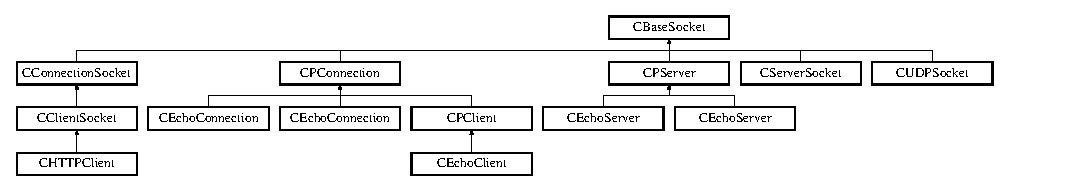
\includegraphics[height=2.137404cm]{class_c_base_socket}
\end{center}
\end{figure}
\subsection*{\-Public \-Member \-Functions}
\begin{DoxyCompactItemize}
\item 
\hyperlink{class_c_base_socket_addf3bf444356a73e1b22b267ffcc3cae}{\-C\-Base\-Socket} ()
\begin{DoxyCompactList}\small\item\em constructor \end{DoxyCompactList}\item 
virtual \hyperlink{class_c_base_socket_affd9b0d8c2917fdc30ff421217ef3c0f}{$\sim$\-C\-Base\-Socket} ()
\item 
virtual \hyperlink{_cpclient_8h_a3be13892ae7076009afcf121347dd319}{\-B\-O\-O\-L} \hyperlink{class_c_base_socket_a5878eecb66f93fe57956656abf048f7d}{\-Create} (int af, int type, int protocol, \hyperlink{_x_plat_8h_a45c20c14d3d8790a22153d08ab2eb2ff}{\-U\-I\-N\-T} n\-Port=0, \hyperlink{_x_plat_8h_a2b72c6037793f6c6381a09c83f27569b}{\-L\-P\-C\-S\-T\-R} lp\-Addr=\-N\-U\-L\-L, \hyperlink{_cpclient_8h_a3be13892ae7076009afcf121347dd319}{\-B\-O\-O\-L} b\-Reuse=\hyperlink{_x_plat_8h_aa93f0eb578d23995850d61f7d61c55c1}{\-F\-A\-L\-S\-E}, \hyperlink{_cpclient_8h_a3be13892ae7076009afcf121347dd319}{\-B\-O\-O\-L} b\-Bind=\hyperlink{_x_plat_8h_aa8cecfc5c5c054d2875c03e77b7be15d}{\-T\-R\-U\-E}, int i\-Linger=-\/1, \hyperlink{_cpclient_8h_a3be13892ae7076009afcf121347dd319}{\-B\-O\-O\-L} b\-No\-Tcp\-Delay=\hyperlink{_x_plat_8h_aa93f0eb578d23995850d61f7d61c55c1}{\-F\-A\-L\-S\-E})
\begin{DoxyCompactList}\small\item\em methods \end{DoxyCompactList}\item 
virtual \hyperlink{_cpclient_8h_a3be13892ae7076009afcf121347dd319}{\-B\-O\-O\-L} \hyperlink{class_c_base_socket_a65ed29350c1d78a6691404738c07b2c2}{\-Set\-Blocking\-Mode} (\hyperlink{_cpclient_8h_a3be13892ae7076009afcf121347dd319}{\-B\-O\-O\-L} b\-Block=\hyperlink{_x_plat_8h_aa8cecfc5c5c054d2875c03e77b7be15d}{\-T\-R\-U\-E})
\begin{DoxyCompactList}\small\item\em \-Make this a blocking socket. \end{DoxyCompactList}\item 
virtual \hyperlink{_cpclient_8h_a6464f7480a0fd0ee170cba12b2c0497f}{void} \hyperlink{class_c_base_socket_ad1e45ab8be1fda6f91704a7159a0a8e4}{\-Close\-Socket} ()
\begin{DoxyCompactList}\small\item\em \-Close socket. \end{DoxyCompactList}\item 
virtual struct sockaddr\-\_\-in $\ast$ \hyperlink{class_c_base_socket_a6f955956a1cd1c94c3ba2a80c1fde41a}{\-Get\-Socket\-Name} ()
\begin{DoxyCompactList}\small\item\em \-Return a socket address structure with info currently bound to the socket. \end{DoxyCompactList}\item 
virtual const char $\ast$ \hyperlink{class_c_base_socket_a78dee8076bd41f62307d70273112b54a}{\-Get\-Socket\-Address\-As\-String} ()
\begin{DoxyCompactList}\small\item\em \-Return the socket address as a string. \end{DoxyCompactList}\item 
virtual int \hyperlink{class_c_base_socket_abae300062e0510d901e2873eface1bc0}{\-Get\-Create\-Error} ()
\begin{DoxyCompactList}\small\item\em \-Return the last create error. \end{DoxyCompactList}\item 
virtual int \hyperlink{class_c_base_socket_a4a6c7866671c019612259f30172cc8c5}{\-Get\-Socket\-Type} ()
\begin{DoxyCompactList}\small\item\em \-Get socket type. \end{DoxyCompactList}\end{DoxyCompactItemize}
\subsection*{\-Protected \-Member \-Functions}
\begin{DoxyCompactItemize}
\item 
virtual \hyperlink{_cpclient_8h_a6464f7480a0fd0ee170cba12b2c0497f}{void} \hyperlink{class_c_base_socket_ab3e4b93f8450b5fa901017d5fddba0e2}{\-Unprotected\-Close\-Socket} ()
\begin{DoxyCompactList}\small\item\em \-Unprotected close socket -\/ called by \-Close\-Socket. \end{DoxyCompactList}\end{DoxyCompactItemize}
\subsection*{\-Protected \-Attributes}
\begin{DoxyCompactItemize}
\item 
\hyperlink{_x_plat_8h_a8dc8083897335125630f1af5dafd5831}{\-S\-O\-C\-K\-E\-T} \hyperlink{class_c_base_socket_a4a40d0e510e311d365681f3af20738b8}{s\-Socket}
\item 
\hyperlink{class_c_x_plat_critical_section}{\-C\-X\-Plat\-Critical\-Section} \hyperlink{class_c_base_socket_ace5626a9274cb3ca77b985e6c5b5af43}{c\-Critical\-Socket}
\item 
\hyperlink{_cpclient_8h_a3be13892ae7076009afcf121347dd319}{\-B\-O\-O\-L} \hyperlink{class_c_base_socket_a57027e1576c0ae6e410c5ccf23724a2d}{b\-Blocking}
\item 
struct sockaddr\-\_\-in \hyperlink{class_c_base_socket_af5f07d3684a2c7876b617885f91a518d}{s\-T\-Addr}
\item 
int \hyperlink{class_c_base_socket_a534d73ca9c9a1a0cd4767efb3b1d0566}{i\-Create\-Error}
\item 
string \hyperlink{class_c_base_socket_af5ea32275a20e337e43689370a9e25ed}{s\-Unix\-Path}
\item 
int \hyperlink{class_c_base_socket_a3f75df97cb5664473c77ec1b323d3407}{i\-A\-F}
\end{DoxyCompactItemize}


\subsection{\-Detailed \-Description}
\-Base socket class implements low level \-Berkley socket functionality. 

\-Definition at line 39 of file \-C\-Base\-Socket.\-h.



\subsection{\-Constructor \& \-Destructor \-Documentation}
\hypertarget{class_c_base_socket_addf3bf444356a73e1b22b267ffcc3cae}{\index{\-C\-Base\-Socket@{\-C\-Base\-Socket}!\-C\-Base\-Socket@{\-C\-Base\-Socket}}
\index{\-C\-Base\-Socket@{\-C\-Base\-Socket}!CBaseSocket@{\-C\-Base\-Socket}}
\subsubsection[{\-C\-Base\-Socket}]{\setlength{\rightskip}{0pt plus 5cm}{\bf \-C\-Base\-Socket\-::\-C\-Base\-Socket} (
\begin{DoxyParamCaption}
{}
\end{DoxyParamCaption}
)}}\label{class_c_base_socket_addf3bf444356a73e1b22b267ffcc3cae}


constructor 



\-Definition at line 32 of file \-C\-Base\-Socket.\-cpp.

\hypertarget{class_c_base_socket_affd9b0d8c2917fdc30ff421217ef3c0f}{\index{\-C\-Base\-Socket@{\-C\-Base\-Socket}!$\sim$\-C\-Base\-Socket@{$\sim$\-C\-Base\-Socket}}
\index{$\sim$\-C\-Base\-Socket@{$\sim$\-C\-Base\-Socket}!CBaseSocket@{\-C\-Base\-Socket}}
\subsubsection[{$\sim$\-C\-Base\-Socket}]{\setlength{\rightskip}{0pt plus 5cm}{\bf \-C\-Base\-Socket\-::$\sim$\-C\-Base\-Socket} (
\begin{DoxyParamCaption}
{}
\end{DoxyParamCaption}
)\hspace{0.3cm}{\ttfamily  \mbox{[}virtual\mbox{]}}}}\label{class_c_base_socket_affd9b0d8c2917fdc30ff421217ef3c0f}


\-Definition at line 39 of file \-C\-Base\-Socket.\-cpp.



\subsection{\-Member \-Function \-Documentation}
\hypertarget{class_c_base_socket_ad1e45ab8be1fda6f91704a7159a0a8e4}{\index{\-C\-Base\-Socket@{\-C\-Base\-Socket}!\-Close\-Socket@{\-Close\-Socket}}
\index{\-Close\-Socket@{\-Close\-Socket}!CBaseSocket@{\-C\-Base\-Socket}}
\subsubsection[{\-Close\-Socket}]{\setlength{\rightskip}{0pt plus 5cm}{\bf void} {\bf \-C\-Base\-Socket\-::\-Close\-Socket} (
\begin{DoxyParamCaption}
{}
\end{DoxyParamCaption}
)\hspace{0.3cm}{\ttfamily  \mbox{[}virtual\mbox{]}}}}\label{class_c_base_socket_ad1e45ab8be1fda6f91704a7159a0a8e4}


\-Close socket. 



\-Reimplemented in \hyperlink{class_c_u_d_p_socket_a4c3f6638dc3c4cbe3ea33ab8b1dd811c}{\-C\-U\-D\-P\-Socket}.



\-Definition at line 207 of file \-C\-Base\-Socket.\-cpp.

\hypertarget{class_c_base_socket_a5878eecb66f93fe57956656abf048f7d}{\index{\-C\-Base\-Socket@{\-C\-Base\-Socket}!\-Create@{\-Create}}
\index{\-Create@{\-Create}!CBaseSocket@{\-C\-Base\-Socket}}
\subsubsection[{\-Create}]{\setlength{\rightskip}{0pt plus 5cm}{\bf \-B\-O\-O\-L} {\bf \-C\-Base\-Socket\-::\-Create} (
\begin{DoxyParamCaption}
\item[{int}]{af, }
\item[{int}]{type, }
\item[{int}]{protocol, }
\item[{{\bf \-U\-I\-N\-T}}]{n\-Port = {\ttfamily 0}, }
\item[{{\bf \-L\-P\-C\-S\-T\-R}}]{lp\-Addr = {\ttfamily \-N\-U\-L\-L}, }
\item[{{\bf \-B\-O\-O\-L}}]{b\-Reuse = {\ttfamily {\bf \-F\-A\-L\-S\-E}}, }
\item[{{\bf \-B\-O\-O\-L}}]{b\-Bind = {\ttfamily {\bf \-T\-R\-U\-E}}, }
\item[{int}]{i\-Linger = {\ttfamily -\/1}, }
\item[{{\bf \-B\-O\-O\-L}}]{b\-No\-Tcp\-Delay = {\ttfamily {\bf \-F\-A\-L\-S\-E}}}
\end{DoxyParamCaption}
)\hspace{0.3cm}{\ttfamily  \mbox{[}virtual\mbox{]}}}}\label{class_c_base_socket_a5878eecb66f93fe57956656abf048f7d}


methods 


\begin{DoxyParams}{\-Parameters}
{\em type} & \-Address family. \-Only tested with \-A\-F\-\_\-\-I\-N\-E\-T. \\
\hline
{\em protocol} & \-Stream or datagram (\-S\-O\-C\-K\-\_\-\-S\-T\-R\-E\-A\-M or \-S\-O\-C\-K\-\_\-\-D\-R\-A\-M) \\
\hline
{\em n\-Port} & \-Usually 0 for inet sockets \\
\hline
{\em lp\-Addr} & \-Port \\
\hline
{\em b\-Reuse} & \-Address. \-For inet in the standard xxx.\-xxx.\-xxx.\-xxx format, for \-A\-F\-\_\-\-U\-N\-I\-X the path \\
\hline
{\em b\-Bind} & \-Allow reuse of this socket \\
\hline
{\em i\-Linger} & \-Default to bind the socket. \-Not needed if this is the result of an \-::accept \\
\hline
{\em b\-No\-Tcp\-Delay} & -\/1 = system default, 0 = \-D\-O\-N\-T\-\_\-\-L\-I\-N\-G\-E\-R, else the timeout \\
\hline
\end{DoxyParams}


\-Definition at line 52 of file \-C\-Base\-Socket.\-cpp.

\hypertarget{class_c_base_socket_abae300062e0510d901e2873eface1bc0}{\index{\-C\-Base\-Socket@{\-C\-Base\-Socket}!\-Get\-Create\-Error@{\-Get\-Create\-Error}}
\index{\-Get\-Create\-Error@{\-Get\-Create\-Error}!CBaseSocket@{\-C\-Base\-Socket}}
\subsubsection[{\-Get\-Create\-Error}]{\setlength{\rightskip}{0pt plus 5cm}int {\bf \-C\-Base\-Socket\-::\-Get\-Create\-Error} (
\begin{DoxyParamCaption}
{}
\end{DoxyParamCaption}
)\hspace{0.3cm}{\ttfamily  \mbox{[}virtual\mbox{]}}}}\label{class_c_base_socket_abae300062e0510d901e2873eface1bc0}


\-Return the last create error. 



\-Definition at line 167 of file \-C\-Base\-Socket.\-cpp.

\hypertarget{class_c_base_socket_a78dee8076bd41f62307d70273112b54a}{\index{\-C\-Base\-Socket@{\-C\-Base\-Socket}!\-Get\-Socket\-Address\-As\-String@{\-Get\-Socket\-Address\-As\-String}}
\index{\-Get\-Socket\-Address\-As\-String@{\-Get\-Socket\-Address\-As\-String}!CBaseSocket@{\-C\-Base\-Socket}}
\subsubsection[{\-Get\-Socket\-Address\-As\-String}]{\setlength{\rightskip}{0pt plus 5cm}const char $\ast$ {\bf \-C\-Base\-Socket\-::\-Get\-Socket\-Address\-As\-String} (
\begin{DoxyParamCaption}
{}
\end{DoxyParamCaption}
)\hspace{0.3cm}{\ttfamily  \mbox{[}virtual\mbox{]}}}}\label{class_c_base_socket_a78dee8076bd41f62307d70273112b54a}


\-Return the socket address as a string. 



\-Definition at line 271 of file \-C\-Base\-Socket.\-cpp.

\hypertarget{class_c_base_socket_a6f955956a1cd1c94c3ba2a80c1fde41a}{\index{\-C\-Base\-Socket@{\-C\-Base\-Socket}!\-Get\-Socket\-Name@{\-Get\-Socket\-Name}}
\index{\-Get\-Socket\-Name@{\-Get\-Socket\-Name}!CBaseSocket@{\-C\-Base\-Socket}}
\subsubsection[{\-Get\-Socket\-Name}]{\setlength{\rightskip}{0pt plus 5cm}struct sockaddr\-\_\-in $\ast$ {\bf \-C\-Base\-Socket\-::\-Get\-Socket\-Name} (
\begin{DoxyParamCaption}
{}
\end{DoxyParamCaption}
)\hspace{0.3cm}{\ttfamily  \mbox{[}read, virtual\mbox{]}}}}\label{class_c_base_socket_a6f955956a1cd1c94c3ba2a80c1fde41a}


\-Return a socket address structure with info currently bound to the socket. 



\-Definition at line 247 of file \-C\-Base\-Socket.\-cpp.

\hypertarget{class_c_base_socket_a4a6c7866671c019612259f30172cc8c5}{\index{\-C\-Base\-Socket@{\-C\-Base\-Socket}!\-Get\-Socket\-Type@{\-Get\-Socket\-Type}}
\index{\-Get\-Socket\-Type@{\-Get\-Socket\-Type}!CBaseSocket@{\-C\-Base\-Socket}}
\subsubsection[{\-Get\-Socket\-Type}]{\setlength{\rightskip}{0pt plus 5cm}int {\bf \-C\-Base\-Socket\-::\-Get\-Socket\-Type} (
\begin{DoxyParamCaption}
{}
\end{DoxyParamCaption}
)\hspace{0.3cm}{\ttfamily  \mbox{[}virtual\mbox{]}}}}\label{class_c_base_socket_a4a6c7866671c019612259f30172cc8c5}


\-Get socket type. 



\-Definition at line 175 of file \-C\-Base\-Socket.\-cpp.

\hypertarget{class_c_base_socket_a65ed29350c1d78a6691404738c07b2c2}{\index{\-C\-Base\-Socket@{\-C\-Base\-Socket}!\-Set\-Blocking\-Mode@{\-Set\-Blocking\-Mode}}
\index{\-Set\-Blocking\-Mode@{\-Set\-Blocking\-Mode}!CBaseSocket@{\-C\-Base\-Socket}}
\subsubsection[{\-Set\-Blocking\-Mode}]{\setlength{\rightskip}{0pt plus 5cm}{\bf \-B\-O\-O\-L} {\bf \-C\-Base\-Socket\-::\-Set\-Blocking\-Mode} (
\begin{DoxyParamCaption}
\item[{{\bf \-B\-O\-O\-L}}]{b\-Block = {\ttfamily {\bf \-T\-R\-U\-E}}}
\end{DoxyParamCaption}
)\hspace{0.3cm}{\ttfamily  \mbox{[}virtual\mbox{]}}}}\label{class_c_base_socket_a65ed29350c1d78a6691404738c07b2c2}


\-Make this a blocking socket. 

\-F\-A\-L\-S\-E = system default, \-T\-R\-U\-E = disable \-Nagle algorithm and send partial data 

\-Definition at line 183 of file \-C\-Base\-Socket.\-cpp.

\hypertarget{class_c_base_socket_ab3e4b93f8450b5fa901017d5fddba0e2}{\index{\-C\-Base\-Socket@{\-C\-Base\-Socket}!\-Unprotected\-Close\-Socket@{\-Unprotected\-Close\-Socket}}
\index{\-Unprotected\-Close\-Socket@{\-Unprotected\-Close\-Socket}!CBaseSocket@{\-C\-Base\-Socket}}
\subsubsection[{\-Unprotected\-Close\-Socket}]{\setlength{\rightskip}{0pt plus 5cm}{\bf void} {\bf \-C\-Base\-Socket\-::\-Unprotected\-Close\-Socket} (
\begin{DoxyParamCaption}
{}
\end{DoxyParamCaption}
)\hspace{0.3cm}{\ttfamily  \mbox{[}protected, virtual\mbox{]}}}}\label{class_c_base_socket_ab3e4b93f8450b5fa901017d5fddba0e2}


\-Unprotected close socket -\/ called by \-Close\-Socket. 



\-Reimplemented in \hyperlink{class_c_p_connection_a5c83da25150fd43d9fe4522d34d6cffb}{\-C\-P\-Connection}.



\-Definition at line 221 of file \-C\-Base\-Socket.\-cpp.



\subsection{\-Member \-Data \-Documentation}
\hypertarget{class_c_base_socket_a57027e1576c0ae6e410c5ccf23724a2d}{\index{\-C\-Base\-Socket@{\-C\-Base\-Socket}!b\-Blocking@{b\-Blocking}}
\index{b\-Blocking@{b\-Blocking}!CBaseSocket@{\-C\-Base\-Socket}}
\subsubsection[{b\-Blocking}]{\setlength{\rightskip}{0pt plus 5cm}{\bf \-B\-O\-O\-L} {\bf \-C\-Base\-Socket\-::b\-Blocking}\hspace{0.3cm}{\ttfamily  \mbox{[}protected\mbox{]}}}}\label{class_c_base_socket_a57027e1576c0ae6e410c5ccf23724a2d}


\-Definition at line 76 of file \-C\-Base\-Socket.\-h.

\hypertarget{class_c_base_socket_ace5626a9274cb3ca77b985e6c5b5af43}{\index{\-C\-Base\-Socket@{\-C\-Base\-Socket}!c\-Critical\-Socket@{c\-Critical\-Socket}}
\index{c\-Critical\-Socket@{c\-Critical\-Socket}!CBaseSocket@{\-C\-Base\-Socket}}
\subsubsection[{c\-Critical\-Socket}]{\setlength{\rightskip}{0pt plus 5cm}{\bf \-C\-X\-Plat\-Critical\-Section} {\bf \-C\-Base\-Socket\-::c\-Critical\-Socket}\hspace{0.3cm}{\ttfamily  \mbox{[}protected\mbox{]}}}}\label{class_c_base_socket_ace5626a9274cb3ca77b985e6c5b5af43}


\-Definition at line 75 of file \-C\-Base\-Socket.\-h.

\hypertarget{class_c_base_socket_a3f75df97cb5664473c77ec1b323d3407}{\index{\-C\-Base\-Socket@{\-C\-Base\-Socket}!i\-A\-F@{i\-A\-F}}
\index{i\-A\-F@{i\-A\-F}!CBaseSocket@{\-C\-Base\-Socket}}
\subsubsection[{i\-A\-F}]{\setlength{\rightskip}{0pt plus 5cm}int {\bf \-C\-Base\-Socket\-::i\-A\-F}\hspace{0.3cm}{\ttfamily  \mbox{[}protected\mbox{]}}}}\label{class_c_base_socket_a3f75df97cb5664473c77ec1b323d3407}


\-Definition at line 80 of file \-C\-Base\-Socket.\-h.

\hypertarget{class_c_base_socket_a534d73ca9c9a1a0cd4767efb3b1d0566}{\index{\-C\-Base\-Socket@{\-C\-Base\-Socket}!i\-Create\-Error@{i\-Create\-Error}}
\index{i\-Create\-Error@{i\-Create\-Error}!CBaseSocket@{\-C\-Base\-Socket}}
\subsubsection[{i\-Create\-Error}]{\setlength{\rightskip}{0pt plus 5cm}int {\bf \-C\-Base\-Socket\-::i\-Create\-Error}\hspace{0.3cm}{\ttfamily  \mbox{[}protected\mbox{]}}}}\label{class_c_base_socket_a534d73ca9c9a1a0cd4767efb3b1d0566}


\-Definition at line 78 of file \-C\-Base\-Socket.\-h.

\hypertarget{class_c_base_socket_a4a40d0e510e311d365681f3af20738b8}{\index{\-C\-Base\-Socket@{\-C\-Base\-Socket}!s\-Socket@{s\-Socket}}
\index{s\-Socket@{s\-Socket}!CBaseSocket@{\-C\-Base\-Socket}}
\subsubsection[{s\-Socket}]{\setlength{\rightskip}{0pt plus 5cm}{\bf \-S\-O\-C\-K\-E\-T} {\bf \-C\-Base\-Socket\-::s\-Socket}\hspace{0.3cm}{\ttfamily  \mbox{[}protected\mbox{]}}}}\label{class_c_base_socket_a4a40d0e510e311d365681f3af20738b8}


\-Definition at line 74 of file \-C\-Base\-Socket.\-h.

\hypertarget{class_c_base_socket_af5f07d3684a2c7876b617885f91a518d}{\index{\-C\-Base\-Socket@{\-C\-Base\-Socket}!s\-T\-Addr@{s\-T\-Addr}}
\index{s\-T\-Addr@{s\-T\-Addr}!CBaseSocket@{\-C\-Base\-Socket}}
\subsubsection[{s\-T\-Addr}]{\setlength{\rightskip}{0pt plus 5cm}struct sockaddr\-\_\-in {\bf \-C\-Base\-Socket\-::s\-T\-Addr}\hspace{0.3cm}{\ttfamily  \mbox{[}protected\mbox{]}}}}\label{class_c_base_socket_af5f07d3684a2c7876b617885f91a518d}


\-Definition at line 77 of file \-C\-Base\-Socket.\-h.

\hypertarget{class_c_base_socket_af5ea32275a20e337e43689370a9e25ed}{\index{\-C\-Base\-Socket@{\-C\-Base\-Socket}!s\-Unix\-Path@{s\-Unix\-Path}}
\index{s\-Unix\-Path@{s\-Unix\-Path}!CBaseSocket@{\-C\-Base\-Socket}}
\subsubsection[{s\-Unix\-Path}]{\setlength{\rightskip}{0pt plus 5cm}string {\bf \-C\-Base\-Socket\-::s\-Unix\-Path}\hspace{0.3cm}{\ttfamily  \mbox{[}protected\mbox{]}}}}\label{class_c_base_socket_af5ea32275a20e337e43689370a9e25ed}


\-Definition at line 79 of file \-C\-Base\-Socket.\-h.



\-The documentation for this class was generated from the following files\-:\begin{DoxyCompactItemize}
\item 
common/\hyperlink{_c_base_socket_8h}{\-C\-Base\-Socket.\-h}\item 
common/\hyperlink{_c_base_socket_8cpp}{\-C\-Base\-Socket.\-cpp}\end{DoxyCompactItemize}

\hypertarget{class_c_client_socket}{\section{\-C\-Client\-Socket \-Class \-Reference}
\label{class_c_client_socket}\index{\-C\-Client\-Socket@{\-C\-Client\-Socket}}
}


\-Client socket.  




{\ttfamily \#include $<$\-C\-Client\-Socket.\-h$>$}

\-Inheritance diagram for \-C\-Client\-Socket\-:\begin{figure}[H]
\begin{center}
\leavevmode
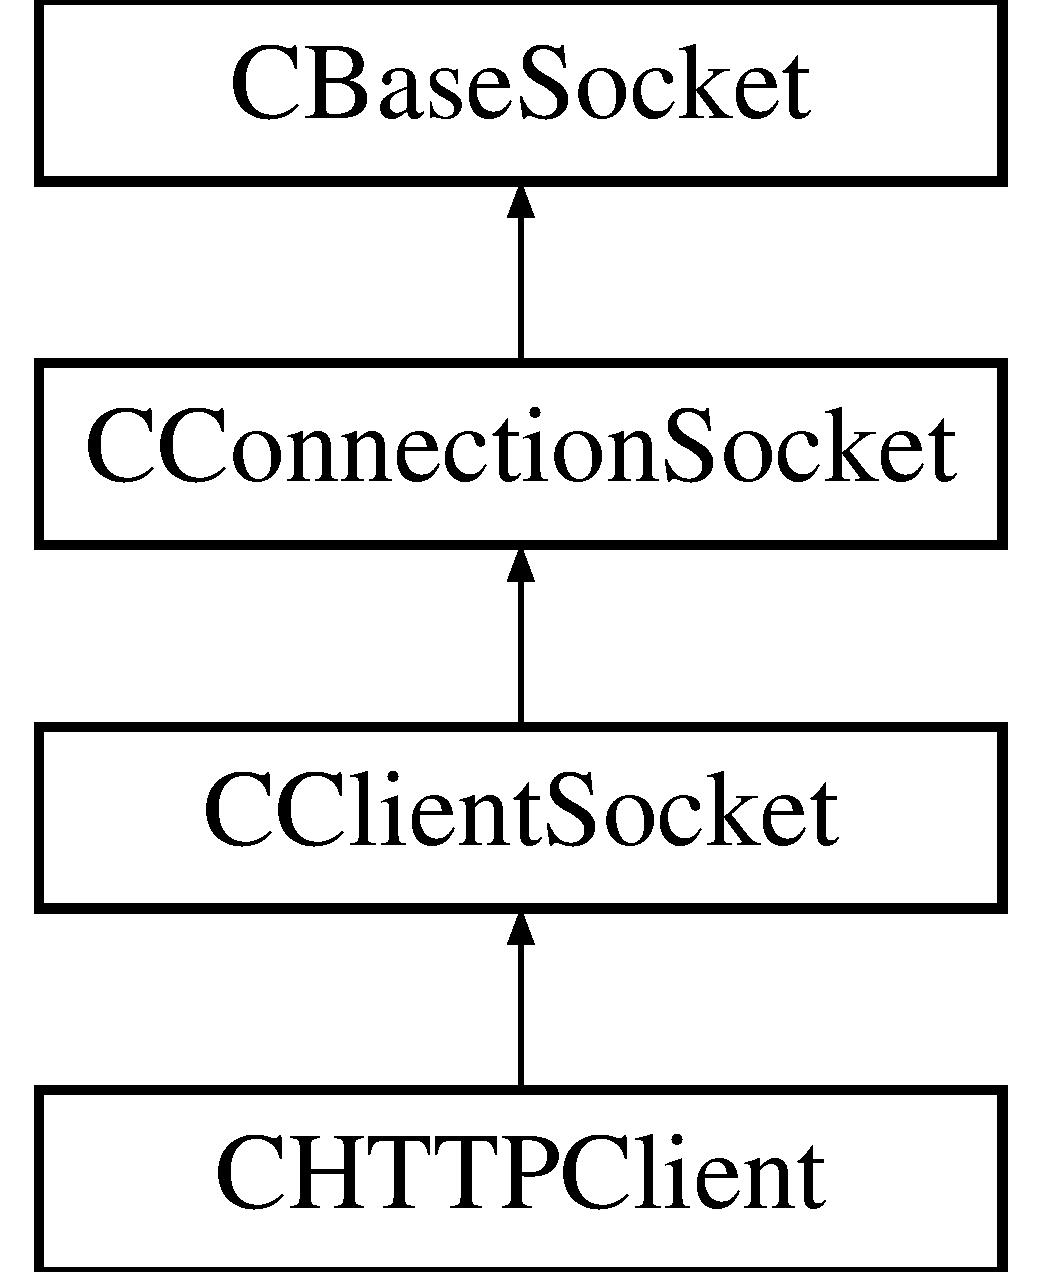
\includegraphics[height=4.000000cm]{class_c_client_socket}
\end{center}
\end{figure}
\subsection*{\-Public \-Member \-Functions}
\begin{DoxyCompactItemize}
\item 
\hyperlink{class_c_client_socket_a45648796359fcb9e67ac9ba9d8ab6879}{\-C\-Client\-Socket} ()
\begin{DoxyCompactList}\small\item\em constructor \end{DoxyCompactList}\item 
virtual \hyperlink{class_c_client_socket_ad9df1bce627d694f3786d801c57eea3c}{$\sim$\-C\-Client\-Socket} ()
\item 
virtual \hyperlink{_cpclient_8h_a3be13892ae7076009afcf121347dd319}{\-B\-O\-O\-L} \hyperlink{class_c_client_socket_ae9e27a8e37cb259cbb37357d763fe9db}{\-Connect\-To\-Server} (\hyperlink{_x_plat_8h_a2b72c6037793f6c6381a09c83f27569b}{\-L\-P\-C\-S\-T\-R} lpsz\-Host\-Address, \hyperlink{_x_plat_8h_a45c20c14d3d8790a22153d08ab2eb2ff}{\-U\-I\-N\-T} n\-Host\-Port, \hyperlink{_x_plat_8h_aa39b39d94407451a6ec0226479db68cf}{\-D\-W\-O\-R\-D} dw\-Timeout=\hyperlink{_x_plat_8h_aa84a29002ab81c719c0d07bb446296e0}{\-I\-N\-F\-I\-N\-I\-T\-E})
\item 
virtual \hyperlink{_cpclient_8h_a3be13892ae7076009afcf121347dd319}{\-B\-O\-O\-L} \hyperlink{class_c_client_socket_a0967869371faa1328e38f9f83d4e9254}{\-Connect\-To\-Unix\-Server} (const char $\ast$sz\-Unix\-Socket, \hyperlink{_x_plat_8h_aa39b39d94407451a6ec0226479db68cf}{\-D\-W\-O\-R\-D} dw\-Timeout=\hyperlink{_x_plat_8h_aa84a29002ab81c719c0d07bb446296e0}{\-I\-N\-F\-I\-N\-I\-T\-E})
\item 
time\-\_\-t \hyperlink{class_c_client_socket_acc44530fac9dd8dc3c648c7a32365750}{\-Get\-Time\-Started} ()
\item 
virtual int \hyperlink{class_c_client_socket_a9ac6b495a4429b4f876f939e0e662104}{\-Get\-Connection\-Error} ()
\begin{DoxyCompactList}\small\item\em \-Last error reported. \end{DoxyCompactList}\item 
\hyperlink{_cpclient_8h_a6464f7480a0fd0ee170cba12b2c0497f}{void} \hyperlink{class_c_client_socket_a45520b4cfcf758dc003877853acf47f7}{\-Set\-Options} (bool \hyperlink{class_c_client_socket_a637cd103e13587df34c0d1937e95aefa}{b\-Reuse}, int \hyperlink{class_c_client_socket_af33729182418c1e9868ad0fed1a68a1e}{i\-Linger}, bool \hyperlink{class_c_client_socket_a0b7201c5883116b700d19bcfc61e49c5}{b\-Tcp\-No\-Delay}=false)
\end{DoxyCompactItemize}
\subsection*{\-Protected \-Member \-Functions}
\begin{DoxyCompactItemize}
\item 
virtual \hyperlink{_cpclient_8h_a3be13892ae7076009afcf121347dd319}{\-B\-O\-O\-L} \hyperlink{class_c_client_socket_a15b0347d2f84e4cd159c981b3ccced47}{\-Attempt\-Connection} ()
\begin{DoxyCompactList}\small\item\em \-Process connections. \end{DoxyCompactList}\item 
virtual \hyperlink{_cpclient_8h_a3be13892ae7076009afcf121347dd319}{\-B\-O\-O\-L} \hyperlink{class_c_client_socket_a5756e507a9decec591fd607dd34e3a85}{\-Initiate\-Connection} ()
\begin{DoxyCompactList}\small\item\em \-Spawn the connection thread. \end{DoxyCompactList}\item 
virtual \hyperlink{_cpclient_8h_a3be13892ae7076009afcf121347dd319}{\-B\-O\-O\-L} \hyperlink{class_c_client_socket_a49f5369ae8f86af2b6adcd44517964fc}{\-Last\-Connect\-Attempt\-Successful} ()
\begin{DoxyCompactList}\small\item\em \-Connect attempt successful? \end{DoxyCompactList}\item 
virtual \hyperlink{_cpclient_8h_a3be13892ae7076009afcf121347dd319}{\-B\-O\-O\-L} \hyperlink{class_c_client_socket_a335a875fe14301b767049bb5d7f72b6f}{\-Connect\-Dispatcher} (\hyperlink{_x_plat_8h_aa39b39d94407451a6ec0226479db68cf}{\-D\-W\-O\-R\-D} dw\-Timeout)
\begin{DoxyCompactList}\small\item\em \-Distribute to either the \-T\-C\-P or \-U\-N\-I\-X connection code. \end{DoxyCompactList}\end{DoxyCompactItemize}
\subsection*{\-Static \-Protected \-Member \-Functions}
\begin{DoxyCompactItemize}
\item 
static unsigned \hyperlink{class_c_client_socket_a115aa8b14c8685a9f71ecc0b30bed3f6}{\-Connect\-Thread} (\hyperlink{_cpclient_8h_a6464f7480a0fd0ee170cba12b2c0497f}{void} $\ast$p\-Void)
\begin{DoxyCompactList}\small\item\em \-Client connect thread. \end{DoxyCompactList}\end{DoxyCompactItemize}
\subsection*{\-Protected \-Attributes}
\begin{DoxyCompactItemize}
\item 
\hyperlink{_cpclient_8h_a3be13892ae7076009afcf121347dd319}{\-B\-O\-O\-L} \hyperlink{class_c_client_socket_added75c4c526045e911bbc732f7d3d25}{b\-Destroying}
\begin{DoxyCompactList}\small\item\em \-Actually does the work. \end{DoxyCompactList}\item 
time\-\_\-t \hyperlink{class_c_client_socket_a64622c72994fb5bcacb0f9e1adf3f080}{t\-Started}
\item 
\hyperlink{_x_plat_8h_af3c5c1485bb09f4be888d78cdaf93e00}{\-X\-P\-L\-A\-T\-\_\-\-H\-A\-N\-D\-L\-E} \hyperlink{class_c_client_socket_a6ce77be76b474ae73e419ea9c89c0b77}{h\-Client\-Thread}
\item 
\hyperlink{_cpclient_8h_a3be13892ae7076009afcf121347dd319}{\-B\-O\-O\-L} \hyperlink{class_c_client_socket_a4d9d11fa1ce3dd3eff8bf0f03afe01ef}{b\-Connect\-Attempt}
\item 
int \hyperlink{class_c_client_socket_a09188be04cc0f1d2c2efa06cd69d8aa1}{i\-Connect\-Error}
\item 
bool \hyperlink{class_c_client_socket_a637cd103e13587df34c0d1937e95aefa}{b\-Reuse}
\item 
int \hyperlink{class_c_client_socket_af33729182418c1e9868ad0fed1a68a1e}{i\-Linger}
\item 
bool \hyperlink{class_c_client_socket_a0b7201c5883116b700d19bcfc61e49c5}{b\-Tcp\-No\-Delay}
\item 
\hyperlink{class_c_x_plat_critical_section}{\-C\-X\-Plat\-Critical\-Section} \hyperlink{class_c_client_socket_a9bb4b1a7b04a8acc551d156c76a6c5ed}{c\-Crit\-Section}
\item 
\hyperlink{class_c_x_plat_event}{\-C\-X\-Plat\-Event} \hyperlink{class_c_client_socket_a9e119c8e8534aac4d7686469429e14b9}{c\-Connect\-Thread\-Done\-Event}
\end{DoxyCompactItemize}


\subsection{\-Detailed \-Description}
\-Client socket. 

\-Implements a client connection. \-You should derive a class from this class which implements a \-Process\-Data method for incoming data and also some external method for sending data (internally, you can use the \-Send\-Data\-Out method). 

\-Definition at line 34 of file \-C\-Client\-Socket.\-h.



\subsection{\-Constructor \& \-Destructor \-Documentation}
\hypertarget{class_c_client_socket_a45648796359fcb9e67ac9ba9d8ab6879}{\index{\-C\-Client\-Socket@{\-C\-Client\-Socket}!\-C\-Client\-Socket@{\-C\-Client\-Socket}}
\index{\-C\-Client\-Socket@{\-C\-Client\-Socket}!CClientSocket@{\-C\-Client\-Socket}}
\subsubsection[{\-C\-Client\-Socket}]{\setlength{\rightskip}{0pt plus 5cm}{\bf \-C\-Client\-Socket\-::\-C\-Client\-Socket} (
\begin{DoxyParamCaption}
{}
\end{DoxyParamCaption}
)}}\label{class_c_client_socket_a45648796359fcb9e67ac9ba9d8ab6879}


constructor 



\-Definition at line 33 of file \-C\-Client\-Socket.\-cpp.

\hypertarget{class_c_client_socket_ad9df1bce627d694f3786d801c57eea3c}{\index{\-C\-Client\-Socket@{\-C\-Client\-Socket}!$\sim$\-C\-Client\-Socket@{$\sim$\-C\-Client\-Socket}}
\index{$\sim$\-C\-Client\-Socket@{$\sim$\-C\-Client\-Socket}!CClientSocket@{\-C\-Client\-Socket}}
\subsubsection[{$\sim$\-C\-Client\-Socket}]{\setlength{\rightskip}{0pt plus 5cm}{\bf \-C\-Client\-Socket\-::$\sim$\-C\-Client\-Socket} (
\begin{DoxyParamCaption}
{}
\end{DoxyParamCaption}
)\hspace{0.3cm}{\ttfamily  \mbox{[}virtual\mbox{]}}}}\label{class_c_client_socket_ad9df1bce627d694f3786d801c57eea3c}


\-Definition at line 43 of file \-C\-Client\-Socket.\-cpp.



\subsection{\-Member \-Function \-Documentation}
\hypertarget{class_c_client_socket_a15b0347d2f84e4cd159c981b3ccced47}{\index{\-C\-Client\-Socket@{\-C\-Client\-Socket}!\-Attempt\-Connection@{\-Attempt\-Connection}}
\index{\-Attempt\-Connection@{\-Attempt\-Connection}!CClientSocket@{\-C\-Client\-Socket}}
\subsubsection[{\-Attempt\-Connection}]{\setlength{\rightskip}{0pt plus 5cm}{\bf \-B\-O\-O\-L} {\bf \-C\-Client\-Socket\-::\-Attempt\-Connection} (
\begin{DoxyParamCaption}
{}
\end{DoxyParamCaption}
)\hspace{0.3cm}{\ttfamily  \mbox{[}protected, virtual\mbox{]}}}}\label{class_c_client_socket_a15b0347d2f84e4cd159c981b3ccced47}


\-Process connections. 



\-Definition at line 333 of file \-C\-Client\-Socket.\-cpp.

\hypertarget{class_c_client_socket_a335a875fe14301b767049bb5d7f72b6f}{\index{\-C\-Client\-Socket@{\-C\-Client\-Socket}!\-Connect\-Dispatcher@{\-Connect\-Dispatcher}}
\index{\-Connect\-Dispatcher@{\-Connect\-Dispatcher}!CClientSocket@{\-C\-Client\-Socket}}
\subsubsection[{\-Connect\-Dispatcher}]{\setlength{\rightskip}{0pt plus 5cm}{\bf \-B\-O\-O\-L} {\bf \-C\-Client\-Socket\-::\-Connect\-Dispatcher} (
\begin{DoxyParamCaption}
\item[{{\bf \-D\-W\-O\-R\-D}}]{dw\-Timeout}
\end{DoxyParamCaption}
)\hspace{0.3cm}{\ttfamily  \mbox{[}protected, virtual\mbox{]}}}}\label{class_c_client_socket_a335a875fe14301b767049bb5d7f72b6f}


\-Distribute to either the \-T\-C\-P or \-U\-N\-I\-X connection code. 



\-Definition at line 77 of file \-C\-Client\-Socket.\-cpp.

\hypertarget{class_c_client_socket_a115aa8b14c8685a9f71ecc0b30bed3f6}{\index{\-C\-Client\-Socket@{\-C\-Client\-Socket}!\-Connect\-Thread@{\-Connect\-Thread}}
\index{\-Connect\-Thread@{\-Connect\-Thread}!CClientSocket@{\-C\-Client\-Socket}}
\subsubsection[{\-Connect\-Thread}]{\setlength{\rightskip}{0pt plus 5cm}unsigned {\bf \-C\-Client\-Socket\-::\-Connect\-Thread} (
\begin{DoxyParamCaption}
\item[{{\bf void} $\ast$}]{p\-Void}
\end{DoxyParamCaption}
)\hspace{0.3cm}{\ttfamily  \mbox{[}static, protected\mbox{]}}}}\label{class_c_client_socket_a115aa8b14c8685a9f71ecc0b30bed3f6}


\-Client connect thread. 



\-Definition at line 316 of file \-C\-Client\-Socket.\-cpp.

\hypertarget{class_c_client_socket_ae9e27a8e37cb259cbb37357d763fe9db}{\index{\-C\-Client\-Socket@{\-C\-Client\-Socket}!\-Connect\-To\-Server@{\-Connect\-To\-Server}}
\index{\-Connect\-To\-Server@{\-Connect\-To\-Server}!CClientSocket@{\-C\-Client\-Socket}}
\subsubsection[{\-Connect\-To\-Server}]{\setlength{\rightskip}{0pt plus 5cm}{\bf \-B\-O\-O\-L} {\bf \-C\-Client\-Socket\-::\-Connect\-To\-Server} (
\begin{DoxyParamCaption}
\item[{{\bf \-L\-P\-C\-S\-T\-R}}]{lpsz\-Host\-Address, }
\item[{{\bf \-U\-I\-N\-T}}]{n\-Host\-Port, }
\item[{{\bf \-D\-W\-O\-R\-D}}]{dw\-Timeout = {\ttfamily {\bf \-I\-N\-F\-I\-N\-I\-T\-E}}}
\end{DoxyParamCaption}
)\hspace{0.3cm}{\ttfamily  \mbox{[}virtual\mbox{]}}}}\label{class_c_client_socket_ae9e27a8e37cb259cbb37357d763fe9db}
\-Connect to a server \-W\-A\-R\-N\-I\-N\-G -\/ if you are going to reuse this object for multiple connections, then you \-M\-U\-S\-T call \-Terminate\-Connection after each connection transaction is complete to clean up resources. 

\-Definition at line 197 of file \-C\-Client\-Socket.\-cpp.

\hypertarget{class_c_client_socket_a0967869371faa1328e38f9f83d4e9254}{\index{\-C\-Client\-Socket@{\-C\-Client\-Socket}!\-Connect\-To\-Unix\-Server@{\-Connect\-To\-Unix\-Server}}
\index{\-Connect\-To\-Unix\-Server@{\-Connect\-To\-Unix\-Server}!CClientSocket@{\-C\-Client\-Socket}}
\subsubsection[{\-Connect\-To\-Unix\-Server}]{\setlength{\rightskip}{0pt plus 5cm}{\bf \-B\-O\-O\-L} {\bf \-C\-Client\-Socket\-::\-Connect\-To\-Unix\-Server} (
\begin{DoxyParamCaption}
\item[{const char $\ast$}]{sz\-Unix\-Socket, }
\item[{{\bf \-D\-W\-O\-R\-D}}]{dw\-Timeout = {\ttfamily {\bf \-I\-N\-F\-I\-N\-I\-T\-E}}}
\end{DoxyParamCaption}
)\hspace{0.3cm}{\ttfamily  \mbox{[}virtual\mbox{]}}}}\label{class_c_client_socket_a0967869371faa1328e38f9f83d4e9254}


\-Definition at line 159 of file \-C\-Client\-Socket.\-cpp.

\hypertarget{class_c_client_socket_a9ac6b495a4429b4f876f939e0e662104}{\index{\-C\-Client\-Socket@{\-C\-Client\-Socket}!\-Get\-Connection\-Error@{\-Get\-Connection\-Error}}
\index{\-Get\-Connection\-Error@{\-Get\-Connection\-Error}!CClientSocket@{\-C\-Client\-Socket}}
\subsubsection[{\-Get\-Connection\-Error}]{\setlength{\rightskip}{0pt plus 5cm}int {\bf \-C\-Client\-Socket\-::\-Get\-Connection\-Error} (
\begin{DoxyParamCaption}
{}
\end{DoxyParamCaption}
)\hspace{0.3cm}{\ttfamily  \mbox{[}virtual\mbox{]}}}}\label{class_c_client_socket_a9ac6b495a4429b4f876f939e0e662104}


\-Last error reported. 



\-Definition at line 368 of file \-C\-Client\-Socket.\-cpp.

\hypertarget{class_c_client_socket_acc44530fac9dd8dc3c648c7a32365750}{\index{\-C\-Client\-Socket@{\-C\-Client\-Socket}!\-Get\-Time\-Started@{\-Get\-Time\-Started}}
\index{\-Get\-Time\-Started@{\-Get\-Time\-Started}!CClientSocket@{\-C\-Client\-Socket}}
\subsubsection[{\-Get\-Time\-Started}]{\setlength{\rightskip}{0pt plus 5cm}time\-\_\-t {\bf \-C\-Client\-Socket\-::\-Get\-Time\-Started} (
\begin{DoxyParamCaption}
{}
\end{DoxyParamCaption}
)}}\label{class_c_client_socket_acc44530fac9dd8dc3c648c7a32365750}


\-Definition at line 266 of file \-C\-Client\-Socket.\-cpp.

\hypertarget{class_c_client_socket_a5756e507a9decec591fd607dd34e3a85}{\index{\-C\-Client\-Socket@{\-C\-Client\-Socket}!\-Initiate\-Connection@{\-Initiate\-Connection}}
\index{\-Initiate\-Connection@{\-Initiate\-Connection}!CClientSocket@{\-C\-Client\-Socket}}
\subsubsection[{\-Initiate\-Connection}]{\setlength{\rightskip}{0pt plus 5cm}{\bf \-B\-O\-O\-L} {\bf \-C\-Client\-Socket\-::\-Initiate\-Connection} (
\begin{DoxyParamCaption}
{}
\end{DoxyParamCaption}
)\hspace{0.3cm}{\ttfamily  \mbox{[}protected, virtual\mbox{]}}}}\label{class_c_client_socket_a5756e507a9decec591fd607dd34e3a85}


\-Spawn the connection thread. 



\-Definition at line 274 of file \-C\-Client\-Socket.\-cpp.

\hypertarget{class_c_client_socket_a49f5369ae8f86af2b6adcd44517964fc}{\index{\-C\-Client\-Socket@{\-C\-Client\-Socket}!\-Last\-Connect\-Attempt\-Successful@{\-Last\-Connect\-Attempt\-Successful}}
\index{\-Last\-Connect\-Attempt\-Successful@{\-Last\-Connect\-Attempt\-Successful}!CClientSocket@{\-C\-Client\-Socket}}
\subsubsection[{\-Last\-Connect\-Attempt\-Successful}]{\setlength{\rightskip}{0pt plus 5cm}{\bf \-B\-O\-O\-L} {\bf \-C\-Client\-Socket\-::\-Last\-Connect\-Attempt\-Successful} (
\begin{DoxyParamCaption}
{}
\end{DoxyParamCaption}
)\hspace{0.3cm}{\ttfamily  \mbox{[}protected, virtual\mbox{]}}}}\label{class_c_client_socket_a49f5369ae8f86af2b6adcd44517964fc}


\-Connect attempt successful? 



\-Definition at line 360 of file \-C\-Client\-Socket.\-cpp.

\hypertarget{class_c_client_socket_a45520b4cfcf758dc003877853acf47f7}{\index{\-C\-Client\-Socket@{\-C\-Client\-Socket}!\-Set\-Options@{\-Set\-Options}}
\index{\-Set\-Options@{\-Set\-Options}!CClientSocket@{\-C\-Client\-Socket}}
\subsubsection[{\-Set\-Options}]{\setlength{\rightskip}{0pt plus 5cm}{\bf void} {\bf \-C\-Client\-Socket\-::\-Set\-Options} (
\begin{DoxyParamCaption}
\item[{bool}]{b\-Reuse, }
\item[{int}]{i\-Linger, }
\item[{bool}]{b\-Tcp\-No\-Delay = {\ttfamily false}}
\end{DoxyParamCaption}
)}}\label{class_c_client_socket_a45520b4cfcf758dc003877853acf47f7}
\-Set socket options -\/ must be called \-B\-E\-F\-O\-R\-E \-Connect\-To\-Server \-Normally, the defaults are fine unless you are going to create and tear down lots of connections 

\-Definition at line 66 of file \-C\-Client\-Socket.\-cpp.



\subsection{\-Member \-Data \-Documentation}
\hypertarget{class_c_client_socket_a4d9d11fa1ce3dd3eff8bf0f03afe01ef}{\index{\-C\-Client\-Socket@{\-C\-Client\-Socket}!b\-Connect\-Attempt@{b\-Connect\-Attempt}}
\index{b\-Connect\-Attempt@{b\-Connect\-Attempt}!CClientSocket@{\-C\-Client\-Socket}}
\subsubsection[{b\-Connect\-Attempt}]{\setlength{\rightskip}{0pt plus 5cm}{\bf \-B\-O\-O\-L} {\bf \-C\-Client\-Socket\-::b\-Connect\-Attempt}\hspace{0.3cm}{\ttfamily  \mbox{[}protected\mbox{]}}}}\label{class_c_client_socket_a4d9d11fa1ce3dd3eff8bf0f03afe01ef}


\-Definition at line 72 of file \-C\-Client\-Socket.\-h.

\hypertarget{class_c_client_socket_added75c4c526045e911bbc732f7d3d25}{\index{\-C\-Client\-Socket@{\-C\-Client\-Socket}!b\-Destroying@{b\-Destroying}}
\index{b\-Destroying@{b\-Destroying}!CClientSocket@{\-C\-Client\-Socket}}
\subsubsection[{b\-Destroying}]{\setlength{\rightskip}{0pt plus 5cm}{\bf \-B\-O\-O\-L} {\bf \-C\-Client\-Socket\-::b\-Destroying}\hspace{0.3cm}{\ttfamily  \mbox{[}protected\mbox{]}}}}\label{class_c_client_socket_added75c4c526045e911bbc732f7d3d25}


\-Actually does the work. 

data member 

\-Definition at line 69 of file \-C\-Client\-Socket.\-h.

\hypertarget{class_c_client_socket_a637cd103e13587df34c0d1937e95aefa}{\index{\-C\-Client\-Socket@{\-C\-Client\-Socket}!b\-Reuse@{b\-Reuse}}
\index{b\-Reuse@{b\-Reuse}!CClientSocket@{\-C\-Client\-Socket}}
\subsubsection[{b\-Reuse}]{\setlength{\rightskip}{0pt plus 5cm}bool {\bf \-C\-Client\-Socket\-::b\-Reuse}\hspace{0.3cm}{\ttfamily  \mbox{[}protected\mbox{]}}}}\label{class_c_client_socket_a637cd103e13587df34c0d1937e95aefa}


\-Definition at line 74 of file \-C\-Client\-Socket.\-h.

\hypertarget{class_c_client_socket_a0b7201c5883116b700d19bcfc61e49c5}{\index{\-C\-Client\-Socket@{\-C\-Client\-Socket}!b\-Tcp\-No\-Delay@{b\-Tcp\-No\-Delay}}
\index{b\-Tcp\-No\-Delay@{b\-Tcp\-No\-Delay}!CClientSocket@{\-C\-Client\-Socket}}
\subsubsection[{b\-Tcp\-No\-Delay}]{\setlength{\rightskip}{0pt plus 5cm}bool {\bf \-C\-Client\-Socket\-::b\-Tcp\-No\-Delay}\hspace{0.3cm}{\ttfamily  \mbox{[}protected\mbox{]}}}}\label{class_c_client_socket_a0b7201c5883116b700d19bcfc61e49c5}


\-Definition at line 76 of file \-C\-Client\-Socket.\-h.

\hypertarget{class_c_client_socket_a9e119c8e8534aac4d7686469429e14b9}{\index{\-C\-Client\-Socket@{\-C\-Client\-Socket}!c\-Connect\-Thread\-Done\-Event@{c\-Connect\-Thread\-Done\-Event}}
\index{c\-Connect\-Thread\-Done\-Event@{c\-Connect\-Thread\-Done\-Event}!CClientSocket@{\-C\-Client\-Socket}}
\subsubsection[{c\-Connect\-Thread\-Done\-Event}]{\setlength{\rightskip}{0pt plus 5cm}{\bf \-C\-X\-Plat\-Event} {\bf \-C\-Client\-Socket\-::c\-Connect\-Thread\-Done\-Event}\hspace{0.3cm}{\ttfamily  \mbox{[}protected\mbox{]}}}}\label{class_c_client_socket_a9e119c8e8534aac4d7686469429e14b9}


\-Definition at line 79 of file \-C\-Client\-Socket.\-h.

\hypertarget{class_c_client_socket_a9bb4b1a7b04a8acc551d156c76a6c5ed}{\index{\-C\-Client\-Socket@{\-C\-Client\-Socket}!c\-Crit\-Section@{c\-Crit\-Section}}
\index{c\-Crit\-Section@{c\-Crit\-Section}!CClientSocket@{\-C\-Client\-Socket}}
\subsubsection[{c\-Crit\-Section}]{\setlength{\rightskip}{0pt plus 5cm}{\bf \-C\-X\-Plat\-Critical\-Section} {\bf \-C\-Client\-Socket\-::c\-Crit\-Section}\hspace{0.3cm}{\ttfamily  \mbox{[}protected\mbox{]}}}}\label{class_c_client_socket_a9bb4b1a7b04a8acc551d156c76a6c5ed}


\-Definition at line 77 of file \-C\-Client\-Socket.\-h.

\hypertarget{class_c_client_socket_a6ce77be76b474ae73e419ea9c89c0b77}{\index{\-C\-Client\-Socket@{\-C\-Client\-Socket}!h\-Client\-Thread@{h\-Client\-Thread}}
\index{h\-Client\-Thread@{h\-Client\-Thread}!CClientSocket@{\-C\-Client\-Socket}}
\subsubsection[{h\-Client\-Thread}]{\setlength{\rightskip}{0pt plus 5cm}{\bf \-X\-P\-L\-A\-T\-\_\-\-H\-A\-N\-D\-L\-E} {\bf \-C\-Client\-Socket\-::h\-Client\-Thread}\hspace{0.3cm}{\ttfamily  \mbox{[}protected\mbox{]}}}}\label{class_c_client_socket_a6ce77be76b474ae73e419ea9c89c0b77}


\-Definition at line 71 of file \-C\-Client\-Socket.\-h.

\hypertarget{class_c_client_socket_a09188be04cc0f1d2c2efa06cd69d8aa1}{\index{\-C\-Client\-Socket@{\-C\-Client\-Socket}!i\-Connect\-Error@{i\-Connect\-Error}}
\index{i\-Connect\-Error@{i\-Connect\-Error}!CClientSocket@{\-C\-Client\-Socket}}
\subsubsection[{i\-Connect\-Error}]{\setlength{\rightskip}{0pt plus 5cm}int {\bf \-C\-Client\-Socket\-::i\-Connect\-Error}\hspace{0.3cm}{\ttfamily  \mbox{[}protected\mbox{]}}}}\label{class_c_client_socket_a09188be04cc0f1d2c2efa06cd69d8aa1}


\-Definition at line 73 of file \-C\-Client\-Socket.\-h.

\hypertarget{class_c_client_socket_af33729182418c1e9868ad0fed1a68a1e}{\index{\-C\-Client\-Socket@{\-C\-Client\-Socket}!i\-Linger@{i\-Linger}}
\index{i\-Linger@{i\-Linger}!CClientSocket@{\-C\-Client\-Socket}}
\subsubsection[{i\-Linger}]{\setlength{\rightskip}{0pt plus 5cm}int {\bf \-C\-Client\-Socket\-::i\-Linger}\hspace{0.3cm}{\ttfamily  \mbox{[}protected\mbox{]}}}}\label{class_c_client_socket_af33729182418c1e9868ad0fed1a68a1e}


\-Definition at line 75 of file \-C\-Client\-Socket.\-h.

\hypertarget{class_c_client_socket_a64622c72994fb5bcacb0f9e1adf3f080}{\index{\-C\-Client\-Socket@{\-C\-Client\-Socket}!t\-Started@{t\-Started}}
\index{t\-Started@{t\-Started}!CClientSocket@{\-C\-Client\-Socket}}
\subsubsection[{t\-Started}]{\setlength{\rightskip}{0pt plus 5cm}time\-\_\-t {\bf \-C\-Client\-Socket\-::t\-Started}\hspace{0.3cm}{\ttfamily  \mbox{[}protected\mbox{]}}}}\label{class_c_client_socket_a64622c72994fb5bcacb0f9e1adf3f080}


\-Definition at line 70 of file \-C\-Client\-Socket.\-h.



\-The documentation for this class was generated from the following files\-:\begin{DoxyCompactItemize}
\item 
common/\hyperlink{_c_client_socket_8h}{\-C\-Client\-Socket.\-h}\item 
common/\hyperlink{_c_client_socket_8cpp}{\-C\-Client\-Socket.\-cpp}\end{DoxyCompactItemize}

\hypertarget{class_c_connection_sig}{\section{\-C\-Connection\-Sig \-Class \-Reference}
\label{class_c_connection_sig}\index{\-C\-Connection\-Sig@{\-C\-Connection\-Sig}}
}


\-Unique signature for each connection.  




{\ttfamily \#include $<$\-C\-P\-Connection.\-h$>$}

\subsection*{\-Public \-Member \-Functions}
\begin{DoxyCompactItemize}
\item 
\hyperlink{class_c_connection_sig_a96cc8d3008e19e3941f77aacedbdadee}{\-C\-Connection\-Sig} ()
\item 
\hyperlink{class_c_connection_sig_a53317c314498d82a97a47f60d7ec5f4a}{$\sim$\-C\-Connection\-Sig} ()
\end{DoxyCompactItemize}
\subsection*{\-Public \-Attributes}
\begin{DoxyCompactItemize}
\item 
\hyperlink{class_c_p_connection}{\-C\-P\-Connection} $\ast$ \hyperlink{class_c_connection_sig_a6941b71b7d8397e19be5cb3996b50aae}{p\-Connection}
\item 
unsigned long \hyperlink{class_c_connection_sig_a8a9b3290adb6c0cabc4f9821a9683a29}{ul\-Time\-Stamp}
\end{DoxyCompactItemize}
\subsection*{\-Friends}
\begin{DoxyCompactItemize}
\item 
bool \hyperlink{class_c_connection_sig_a108267e3b776ae5703cf784ec5307ebb}{operator==} (const \hyperlink{class_c_connection_sig}{\-C\-Connection\-Sig} \&csig1, const \hyperlink{class_c_connection_sig}{\-C\-Connection\-Sig} \&csig2)
\begin{DoxyCompactList}\small\item\em \-Operators. \end{DoxyCompactList}\item 
bool \hyperlink{class_c_connection_sig_a76e8e1e9c79d319028a7003284aa75e1}{operator$<$} (const \hyperlink{class_c_connection_sig}{\-C\-Connection\-Sig} \&csig1, const \hyperlink{class_c_connection_sig}{\-C\-Connection\-Sig} \&csig2)
\item 
bool \hyperlink{class_c_connection_sig_a64a4e21ad9f3fc58a12a9bf787c525be}{operator$>$} (const \hyperlink{class_c_connection_sig}{\-C\-Connection\-Sig} \&csig1, const \hyperlink{class_c_connection_sig}{\-C\-Connection\-Sig} \&csig2)
\end{DoxyCompactItemize}


\subsection{\-Detailed \-Description}
\-Unique signature for each connection. 

\-Definition at line 31 of file \-C\-P\-Connection.\-h.



\subsection{\-Constructor \& \-Destructor \-Documentation}
\hypertarget{class_c_connection_sig_a96cc8d3008e19e3941f77aacedbdadee}{\index{\-C\-Connection\-Sig@{\-C\-Connection\-Sig}!\-C\-Connection\-Sig@{\-C\-Connection\-Sig}}
\index{\-C\-Connection\-Sig@{\-C\-Connection\-Sig}!CConnectionSig@{\-C\-Connection\-Sig}}
\subsubsection[{\-C\-Connection\-Sig}]{\setlength{\rightskip}{0pt plus 5cm}{\bf \-C\-Connection\-Sig\-::\-C\-Connection\-Sig} (
\begin{DoxyParamCaption}
{}
\end{DoxyParamCaption}
)\hspace{0.3cm}{\ttfamily  \mbox{[}inline\mbox{]}}}}\label{class_c_connection_sig_a96cc8d3008e19e3941f77aacedbdadee}


\-Definition at line 35 of file \-C\-P\-Connection.\-h.

\hypertarget{class_c_connection_sig_a53317c314498d82a97a47f60d7ec5f4a}{\index{\-C\-Connection\-Sig@{\-C\-Connection\-Sig}!$\sim$\-C\-Connection\-Sig@{$\sim$\-C\-Connection\-Sig}}
\index{$\sim$\-C\-Connection\-Sig@{$\sim$\-C\-Connection\-Sig}!CConnectionSig@{\-C\-Connection\-Sig}}
\subsubsection[{$\sim$\-C\-Connection\-Sig}]{\setlength{\rightskip}{0pt plus 5cm}{\bf \-C\-Connection\-Sig\-::$\sim$\-C\-Connection\-Sig} (
\begin{DoxyParamCaption}
{}
\end{DoxyParamCaption}
)\hspace{0.3cm}{\ttfamily  \mbox{[}inline\mbox{]}}}}\label{class_c_connection_sig_a53317c314498d82a97a47f60d7ec5f4a}


\-Definition at line 39 of file \-C\-P\-Connection.\-h.



\subsection{\-Friends \-And \-Related \-Function \-Documentation}
\hypertarget{class_c_connection_sig_a76e8e1e9c79d319028a7003284aa75e1}{\index{\-C\-Connection\-Sig@{\-C\-Connection\-Sig}!operator$<$@{operator$<$}}
\index{operator$<$@{operator$<$}!CConnectionSig@{\-C\-Connection\-Sig}}
\subsubsection[{operator$<$}]{\setlength{\rightskip}{0pt plus 5cm}bool operator$<$ (
\begin{DoxyParamCaption}
\item[{const {\bf \-C\-Connection\-Sig} \&}]{csig1, }
\item[{const {\bf \-C\-Connection\-Sig} \&}]{csig2}
\end{DoxyParamCaption}
)\hspace{0.3cm}{\ttfamily  \mbox{[}friend\mbox{]}}}}\label{class_c_connection_sig_a76e8e1e9c79d319028a7003284aa75e1}


\-Definition at line 53 of file \-C\-P\-Connection.\-h.

\hypertarget{class_c_connection_sig_a108267e3b776ae5703cf784ec5307ebb}{\index{\-C\-Connection\-Sig@{\-C\-Connection\-Sig}!operator==@{operator==}}
\index{operator==@{operator==}!CConnectionSig@{\-C\-Connection\-Sig}}
\subsubsection[{operator==}]{\setlength{\rightskip}{0pt plus 5cm}bool operator== (
\begin{DoxyParamCaption}
\item[{const {\bf \-C\-Connection\-Sig} \&}]{csig1, }
\item[{const {\bf \-C\-Connection\-Sig} \&}]{csig2}
\end{DoxyParamCaption}
)\hspace{0.3cm}{\ttfamily  \mbox{[}friend\mbox{]}}}}\label{class_c_connection_sig_a108267e3b776ae5703cf784ec5307ebb}


\-Operators. 



\-Definition at line 45 of file \-C\-P\-Connection.\-h.

\hypertarget{class_c_connection_sig_a64a4e21ad9f3fc58a12a9bf787c525be}{\index{\-C\-Connection\-Sig@{\-C\-Connection\-Sig}!operator$>$@{operator$>$}}
\index{operator$>$@{operator$>$}!CConnectionSig@{\-C\-Connection\-Sig}}
\subsubsection[{operator$>$}]{\setlength{\rightskip}{0pt plus 5cm}bool operator$>$ (
\begin{DoxyParamCaption}
\item[{const {\bf \-C\-Connection\-Sig} \&}]{csig1, }
\item[{const {\bf \-C\-Connection\-Sig} \&}]{csig2}
\end{DoxyParamCaption}
)\hspace{0.3cm}{\ttfamily  \mbox{[}friend\mbox{]}}}}\label{class_c_connection_sig_a64a4e21ad9f3fc58a12a9bf787c525be}


\-Definition at line 62 of file \-C\-P\-Connection.\-h.



\subsection{\-Member \-Data \-Documentation}
\hypertarget{class_c_connection_sig_a6941b71b7d8397e19be5cb3996b50aae}{\index{\-C\-Connection\-Sig@{\-C\-Connection\-Sig}!p\-Connection@{p\-Connection}}
\index{p\-Connection@{p\-Connection}!CConnectionSig@{\-C\-Connection\-Sig}}
\subsubsection[{p\-Connection}]{\setlength{\rightskip}{0pt plus 5cm}{\bf \-C\-P\-Connection}$\ast$ {\bf \-C\-Connection\-Sig\-::p\-Connection}}}\label{class_c_connection_sig_a6941b71b7d8397e19be5cb3996b50aae}


\-Definition at line 69 of file \-C\-P\-Connection.\-h.

\hypertarget{class_c_connection_sig_a8a9b3290adb6c0cabc4f9821a9683a29}{\index{\-C\-Connection\-Sig@{\-C\-Connection\-Sig}!ul\-Time\-Stamp@{ul\-Time\-Stamp}}
\index{ul\-Time\-Stamp@{ul\-Time\-Stamp}!CConnectionSig@{\-C\-Connection\-Sig}}
\subsubsection[{ul\-Time\-Stamp}]{\setlength{\rightskip}{0pt plus 5cm}unsigned long {\bf \-C\-Connection\-Sig\-::ul\-Time\-Stamp}}}\label{class_c_connection_sig_a8a9b3290adb6c0cabc4f9821a9683a29}


\-Definition at line 72 of file \-C\-P\-Connection.\-h.



\-The documentation for this class was generated from the following file\-:\begin{DoxyCompactItemize}
\item 
common/\hyperlink{_c_p_connection_8h}{\-C\-P\-Connection.\-h}\end{DoxyCompactItemize}

\hypertarget{class_c_connection_socket}{\section{\-C\-Connection\-Socket \-Class \-Reference}
\label{class_c_connection_socket}\index{\-C\-Connection\-Socket@{\-C\-Connection\-Socket}}
}


\hyperlink{class_c_connection_socket}{\-C\-Connection\-Socket} -\/ \-Establish a connection with the caller.  




{\ttfamily \#include $<$\-C\-Connection\-Socket.\-h$>$}

\-Inheritance diagram for \-C\-Connection\-Socket\-:\begin{figure}[H]
\begin{center}
\leavevmode
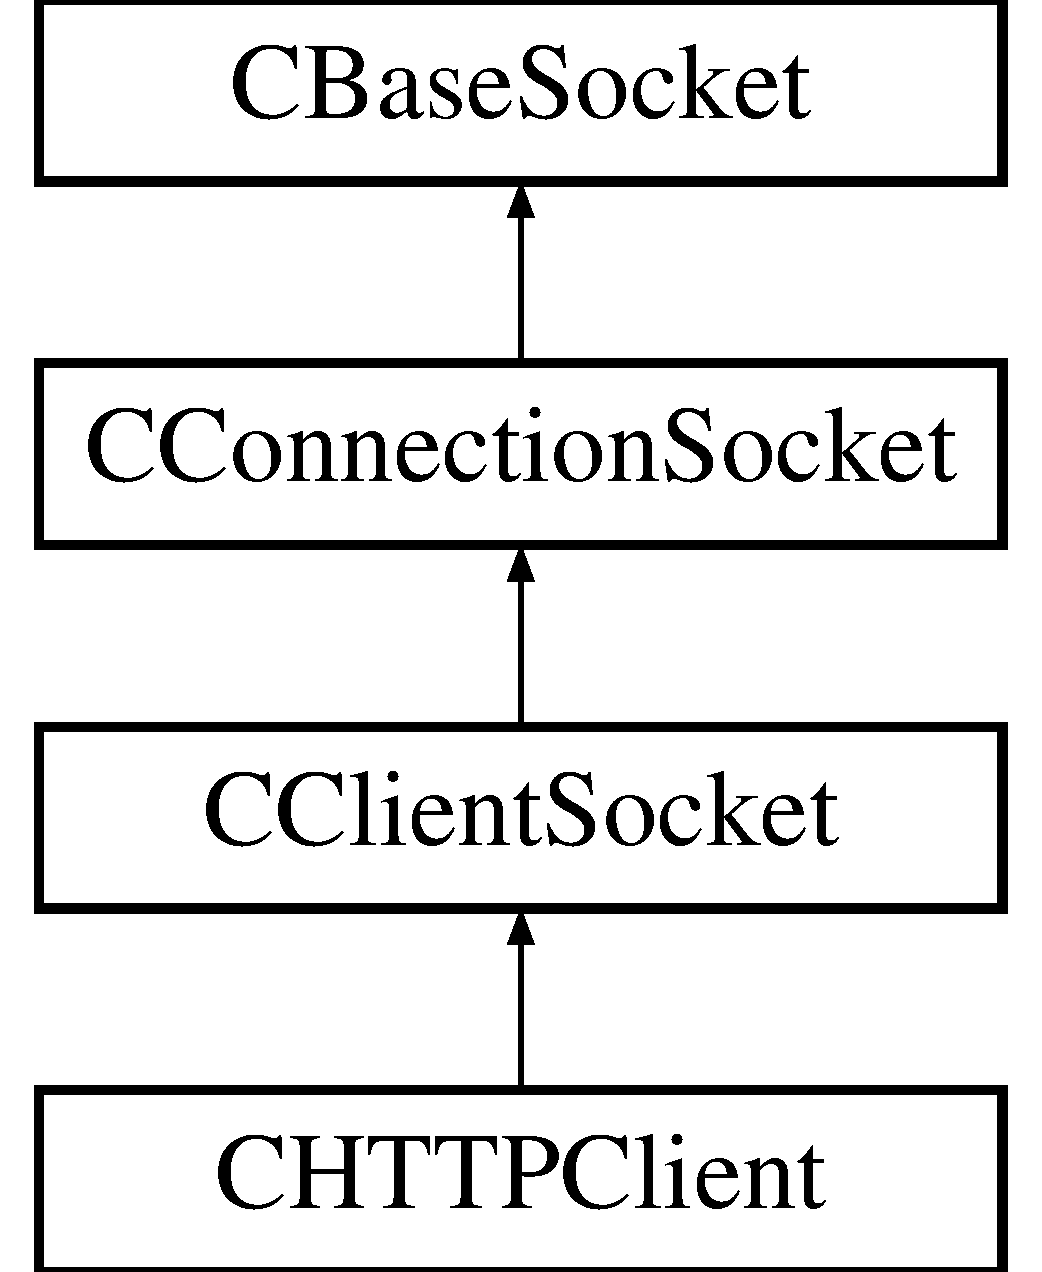
\includegraphics[height=4.000000cm]{class_c_connection_socket}
\end{center}
\end{figure}
\subsection*{\-Public \-Types}
\begin{DoxyCompactItemize}
\item 
enum \{ \hyperlink{class_c_connection_socket_a0d76efb3e65e70281ce2f12dc36dc329a5b96f929feebb30dc72b969542959beb}{\-C\-S\-\_\-\-B\-U\-F\-F\-E\-R\-\_\-\-S\-I\-Z\-E} =  0x2000
 \}
\item 
enum \hyperlink{class_c_connection_socket_a8a17c63c4d0bd7ea0041fbdbd3afc821}{\-E\-C\-L\-O\-S\-E\-\_\-\-T\-Y\-P\-E} \{ \hyperlink{class_c_connection_socket_a8a17c63c4d0bd7ea0041fbdbd3afc821aa4e6154bcc69b59bd3a74ce0c218da3a}{\-C\-L\-O\-S\-E\-\_\-\-A\-C\-T\-I\-V\-E} =  0, 
\hyperlink{class_c_connection_socket_a8a17c63c4d0bd7ea0041fbdbd3afc821a8a49384dfb9d5d199d06bf076294fa95}{\-C\-L\-O\-S\-E\-\_\-\-W\-A\-I\-T} =  1, 
\hyperlink{class_c_connection_socket_a8a17c63c4d0bd7ea0041fbdbd3afc821abe6c0dccf410f304f04098080744411e}{\-C\-L\-O\-S\-E\-\_\-\-I\-M\-M\-E\-D\-I\-A\-T\-E} =  2
 \}
\end{DoxyCompactItemize}
\subsection*{\-Public \-Member \-Functions}
\begin{DoxyCompactItemize}
\item 
\hyperlink{class_c_connection_socket_a738b33d571cd2a09f6570fb576cf9f3d}{\-C\-Connection\-Socket} (\hyperlink{class_c_base_socket}{\-C\-Base\-Socket} $\ast$p\-Owner, struct sockaddr $\ast$p\-Addr=\-N\-U\-L\-L)
\begin{DoxyCompactList}\small\item\em \-Operations. \end{DoxyCompactList}\item 
virtual \hyperlink{class_c_connection_socket_a4b97f20707d0fc603ce11ba98ebd1615}{$\sim$\-C\-Connection\-Socket} ()
\item 
virtual \hyperlink{_x_plat_8h_af3c5c1485bb09f4be888d78cdaf93e00}{\-X\-P\-L\-A\-T\-\_\-\-H\-A\-N\-D\-L\-E} \hyperlink{class_c_connection_socket_ad28950453ac7b8e7763ebd72210a119d}{\-Service\-Connection} (\hyperlink{_x_plat_8h_a8dc8083897335125630f1af5dafd5831}{\-S\-O\-C\-K\-E\-T} s\-New\-Socket)
\begin{DoxyCompactList}\small\item\em \-Methods. \end{DoxyCompactList}\item 
virtual \hyperlink{_cpclient_8h_a6464f7480a0fd0ee170cba12b2c0497f}{void} \hyperlink{class_c_connection_socket_a3d5b3f4e05c9ccd5fe395b2ac923cada}{\-Terminate\-Connection} (\hyperlink{class_c_connection_socket_a8a17c63c4d0bd7ea0041fbdbd3afc821}{\-E\-C\-L\-O\-S\-E\-\_\-\-T\-Y\-P\-E} e\-Request=\hyperlink{class_c_connection_socket_a8a17c63c4d0bd7ea0041fbdbd3afc821a8a49384dfb9d5d199d06bf076294fa95}{\-C\-L\-O\-S\-E\-\_\-\-W\-A\-I\-T})
\begin{DoxyCompactList}\small\item\em \-Closes service thread by closing socket. \end{DoxyCompactList}\item 
virtual time\-\_\-t \hyperlink{class_c_connection_socket_a6193ee146fc12ed536b0b3cf02038fcc}{\-Get\-Time\-Connected} ()
\begin{DoxyCompactList}\small\item\em \-Return the time the connection was initiated. \end{DoxyCompactList}\item 
virtual \hyperlink{_cpclient_8h_a3be13892ae7076009afcf121347dd319}{\-B\-O\-O\-L} \hyperlink{class_c_connection_socket_a3949c412fdb7b529395cc55a13ee6902}{\-Is\-Connected} ()
\begin{DoxyCompactList}\small\item\em \-Connected? \end{DoxyCompactList}\item 
virtual struct sockaddr\-\_\-in \hyperlink{class_c_connection_socket_abee4469b813b7c4430f22ae166b6613a}{\-Get\-Socket\-Address} ()
\begin{DoxyCompactList}\small\item\em \-Get socket address. \end{DoxyCompactList}\end{DoxyCompactItemize}
\subsection*{\-Public \-Attributes}
\begin{DoxyCompactItemize}
\item 
\hyperlink{_x_plat_8h_af3c5c1485bb09f4be888d78cdaf93e00}{\-X\-P\-L\-A\-T\-\_\-\-H\-A\-N\-D\-L\-E} \hyperlink{class_c_connection_socket_af47f017bb0e097654d633fd32da63024}{h\-Thread}
\end{DoxyCompactItemize}
\subsection*{\-Protected \-Member \-Functions}
\begin{DoxyCompactItemize}
\item 
virtual int \hyperlink{class_c_connection_socket_a8ecacc72605561cc4caf0e4e5b1544d3}{\-Receive\-Data} (\hyperlink{_cpclient_8h_a6464f7480a0fd0ee170cba12b2c0497f}{void} $\ast$lp\-Buf, int n\-Buf\-Len)
\begin{DoxyCompactList}\small\item\em \-Receive the data from socket, external buffer. \end{DoxyCompactList}\item 
virtual int \hyperlink{class_c_connection_socket_ae51ffdd227d424b6c3ffdb6c6b79e336}{\-Receive\-Data} ()
\begin{DoxyCompactList}\small\item\em \-Receive the data from socket, internal buffer. \end{DoxyCompactList}\item 
virtual \hyperlink{_cpclient_8h_a3be13892ae7076009afcf121347dd319}{\-B\-O\-O\-L} \hyperlink{class_c_connection_socket_a54eab4ef6efbf0e23f12c45e4784895c}{\-Send\-Data\-Out} (\hyperlink{_x_plat_8h_ad162cb9da5f09788c88e33cd9486a158}{\-L\-P\-S\-T\-R} lp\-Data, int n\-Packet\-Size, int n\-Total\-Length)
\begin{DoxyCompactList}\small\item\em \-Send data. \end{DoxyCompactList}\item 
virtual \hyperlink{_cpclient_8h_a3be13892ae7076009afcf121347dd319}{\-B\-O\-O\-L} \hyperlink{class_c_connection_socket_a11c2aef1e11bbac03c72ec9444b8e85f}{\-Process\-Data} (unsigned char $\ast$lp\-Data, int i\-Len)=0
\begin{DoxyCompactList}\small\item\em \-Pure virtual function to process data. \end{DoxyCompactList}\item 
virtual \hyperlink{_cpclient_8h_a3be13892ae7076009afcf121347dd319}{\-B\-O\-O\-L} \hyperlink{class_c_connection_socket_a413e9745a663ad7de35320d1fb2b6e91}{\-Get\-Handshake} (unsigned char $\ast$$\ast$uc\-H\-S, int \&i\-Len)
\item 
virtual \hyperlink{_cpclient_8h_a6464f7480a0fd0ee170cba12b2c0497f}{void} \hyperlink{class_c_connection_socket_a2d991ece47fd9c86366af981c70d51fc}{\-Disconnected} ()
\begin{DoxyCompactList}\small\item\em \-When the \-Service\-Connection\-Thread stops, this gets called. \end{DoxyCompactList}\item 
virtual int \hyperlink{class_c_connection_socket_a92a2d68cd4df71591df3bd8320777504}{\-Handle\-Connection} ()
\begin{DoxyCompactList}\small\item\em \-Called by \-Service\-Connection\-Thread to actually do the work. \end{DoxyCompactList}\end{DoxyCompactItemize}
\subsection*{\-Static \-Protected \-Member \-Functions}
\begin{DoxyCompactItemize}
\item 
static unsigned \hyperlink{class_c_connection_socket_add0d86dff0967303cb14c0edb5ef8ffe}{\-Service\-Connection\-Thread} (\hyperlink{_cpclient_8h_a6464f7480a0fd0ee170cba12b2c0497f}{void} $\ast$p\-Void)
\begin{DoxyCompactList}\small\item\em \-Thread function to listen to data, etc. \end{DoxyCompactList}\end{DoxyCompactItemize}
\subsection*{\-Protected \-Attributes}
\begin{DoxyCompactItemize}
\item 
unsigned char \hyperlink{class_c_connection_socket_abc2fd15e5e9f2f3e112012bdbe0b5c94}{uc\-Buffer} \mbox{[}\hyperlink{class_c_connection_socket_a0d76efb3e65e70281ce2f12dc36dc329a5b96f929feebb30dc72b969542959beb}{\-C\-S\-\_\-\-B\-U\-F\-F\-E\-R\-\_\-\-S\-I\-Z\-E}\mbox{]}
\item 
\hyperlink{class_c_base_socket}{\-C\-Base\-Socket} $\ast$ \hyperlink{class_c_connection_socket_a0eb429ece7da6cfb9337fcf760087145}{c\-Owner}
\item 
time\-\_\-t \hyperlink{class_c_connection_socket_a831e97fbbea5727f1865f14cda4685cb}{t\-Connected}
\item 
struct sockaddr\-\_\-in \hyperlink{class_c_connection_socket_ad6faf61267b6f4a6f8d389a8bceac45d}{s\-Addr}
\item 
struct sockaddr\-\_\-un \hyperlink{class_c_connection_socket_aee6bfbd64246bf4c8be8b23acb9e124e}{s\-U\-Addr}
\item 
\hyperlink{class_c_connection_socket_a8a17c63c4d0bd7ea0041fbdbd3afc821}{\-E\-C\-L\-O\-S\-E\-\_\-\-T\-Y\-P\-E} \hyperlink{class_c_connection_socket_a60bbd36d27ad2d0efd579243857773ac}{e\-Request\-Close}
\end{DoxyCompactItemize}


\subsection{\-Detailed \-Description}
\hyperlink{class_c_connection_socket}{\-C\-Connection\-Socket} -\/ \-Establish a connection with the caller. 

\-Definition at line 31 of file \-C\-Connection\-Socket.\-h.



\subsection{\-Member \-Enumeration \-Documentation}
\hypertarget{class_c_connection_socket_a0d76efb3e65e70281ce2f12dc36dc329}{\subsubsection[{anonymous enum}]{\setlength{\rightskip}{0pt plus 5cm}anonymous enum}}\label{class_c_connection_socket_a0d76efb3e65e70281ce2f12dc36dc329}
\begin{Desc}
\item[\-Enumerator\-: ]\par
\begin{description}
\index{\-C\-S\-\_\-\-B\-U\-F\-F\-E\-R\-\_\-\-S\-I\-Z\-E@{\-C\-S\-\_\-\-B\-U\-F\-F\-E\-R\-\_\-\-S\-I\-Z\-E}!\-C\-Connection\-Socket@{\-C\-Connection\-Socket}}\index{\-C\-Connection\-Socket@{\-C\-Connection\-Socket}!\-C\-S\-\_\-\-B\-U\-F\-F\-E\-R\-\_\-\-S\-I\-Z\-E@{\-C\-S\-\_\-\-B\-U\-F\-F\-E\-R\-\_\-\-S\-I\-Z\-E}}\item[{\em 
\hypertarget{class_c_connection_socket_a0d76efb3e65e70281ce2f12dc36dc329a5b96f929feebb30dc72b969542959beb}{\-C\-S\-\_\-\-B\-U\-F\-F\-E\-R\-\_\-\-S\-I\-Z\-E}\label{class_c_connection_socket_a0d76efb3e65e70281ce2f12dc36dc329a5b96f929feebb30dc72b969542959beb}
}]\end{description}
\end{Desc}



\-Definition at line 38 of file \-C\-Connection\-Socket.\-h.

\hypertarget{class_c_connection_socket_a8a17c63c4d0bd7ea0041fbdbd3afc821}{\index{\-C\-Connection\-Socket@{\-C\-Connection\-Socket}!\-E\-C\-L\-O\-S\-E\-\_\-\-T\-Y\-P\-E@{\-E\-C\-L\-O\-S\-E\-\_\-\-T\-Y\-P\-E}}
\index{\-E\-C\-L\-O\-S\-E\-\_\-\-T\-Y\-P\-E@{\-E\-C\-L\-O\-S\-E\-\_\-\-T\-Y\-P\-E}!CConnectionSocket@{\-C\-Connection\-Socket}}
\subsubsection[{\-E\-C\-L\-O\-S\-E\-\_\-\-T\-Y\-P\-E}]{\setlength{\rightskip}{0pt plus 5cm}enum {\bf \-C\-Connection\-Socket\-::\-E\-C\-L\-O\-S\-E\-\_\-\-T\-Y\-P\-E}}}\label{class_c_connection_socket_a8a17c63c4d0bd7ea0041fbdbd3afc821}
\begin{Desc}
\item[\-Enumerator\-: ]\par
\begin{description}
\index{\-C\-L\-O\-S\-E\-\_\-\-A\-C\-T\-I\-V\-E@{\-C\-L\-O\-S\-E\-\_\-\-A\-C\-T\-I\-V\-E}!\-C\-Connection\-Socket@{\-C\-Connection\-Socket}}\index{\-C\-Connection\-Socket@{\-C\-Connection\-Socket}!\-C\-L\-O\-S\-E\-\_\-\-A\-C\-T\-I\-V\-E@{\-C\-L\-O\-S\-E\-\_\-\-A\-C\-T\-I\-V\-E}}\item[{\em 
\hypertarget{class_c_connection_socket_a8a17c63c4d0bd7ea0041fbdbd3afc821aa4e6154bcc69b59bd3a74ce0c218da3a}{\-C\-L\-O\-S\-E\-\_\-\-A\-C\-T\-I\-V\-E}\label{class_c_connection_socket_a8a17c63c4d0bd7ea0041fbdbd3afc821aa4e6154bcc69b59bd3a74ce0c218da3a}
}]\index{\-C\-L\-O\-S\-E\-\_\-\-W\-A\-I\-T@{\-C\-L\-O\-S\-E\-\_\-\-W\-A\-I\-T}!\-C\-Connection\-Socket@{\-C\-Connection\-Socket}}\index{\-C\-Connection\-Socket@{\-C\-Connection\-Socket}!\-C\-L\-O\-S\-E\-\_\-\-W\-A\-I\-T@{\-C\-L\-O\-S\-E\-\_\-\-W\-A\-I\-T}}\item[{\em 
\hypertarget{class_c_connection_socket_a8a17c63c4d0bd7ea0041fbdbd3afc821a8a49384dfb9d5d199d06bf076294fa95}{\-C\-L\-O\-S\-E\-\_\-\-W\-A\-I\-T}\label{class_c_connection_socket_a8a17c63c4d0bd7ea0041fbdbd3afc821a8a49384dfb9d5d199d06bf076294fa95}
}]\index{\-C\-L\-O\-S\-E\-\_\-\-I\-M\-M\-E\-D\-I\-A\-T\-E@{\-C\-L\-O\-S\-E\-\_\-\-I\-M\-M\-E\-D\-I\-A\-T\-E}!\-C\-Connection\-Socket@{\-C\-Connection\-Socket}}\index{\-C\-Connection\-Socket@{\-C\-Connection\-Socket}!\-C\-L\-O\-S\-E\-\_\-\-I\-M\-M\-E\-D\-I\-A\-T\-E@{\-C\-L\-O\-S\-E\-\_\-\-I\-M\-M\-E\-D\-I\-A\-T\-E}}\item[{\em 
\hypertarget{class_c_connection_socket_a8a17c63c4d0bd7ea0041fbdbd3afc821abe6c0dccf410f304f04098080744411e}{\-C\-L\-O\-S\-E\-\_\-\-I\-M\-M\-E\-D\-I\-A\-T\-E}\label{class_c_connection_socket_a8a17c63c4d0bd7ea0041fbdbd3afc821abe6c0dccf410f304f04098080744411e}
}]\end{description}
\end{Desc}



\-Definition at line 42 of file \-C\-Connection\-Socket.\-h.



\subsection{\-Constructor \& \-Destructor \-Documentation}
\hypertarget{class_c_connection_socket_a738b33d571cd2a09f6570fb576cf9f3d}{\index{\-C\-Connection\-Socket@{\-C\-Connection\-Socket}!\-C\-Connection\-Socket@{\-C\-Connection\-Socket}}
\index{\-C\-Connection\-Socket@{\-C\-Connection\-Socket}!CConnectionSocket@{\-C\-Connection\-Socket}}
\subsubsection[{\-C\-Connection\-Socket}]{\setlength{\rightskip}{0pt plus 5cm}{\bf \-C\-Connection\-Socket\-::\-C\-Connection\-Socket} (
\begin{DoxyParamCaption}
\item[{{\bf \-C\-Base\-Socket} $\ast$}]{p\-Owner, }
\item[{struct sockaddr $\ast$}]{p\-Addr = {\ttfamily \-N\-U\-L\-L}}
\end{DoxyParamCaption}
)}}\label{class_c_connection_socket_a738b33d571cd2a09f6570fb576cf9f3d}


\-Operations. 



\-Definition at line 32 of file \-C\-Connection\-Socket.\-cpp.

\hypertarget{class_c_connection_socket_a4b97f20707d0fc603ce11ba98ebd1615}{\index{\-C\-Connection\-Socket@{\-C\-Connection\-Socket}!$\sim$\-C\-Connection\-Socket@{$\sim$\-C\-Connection\-Socket}}
\index{$\sim$\-C\-Connection\-Socket@{$\sim$\-C\-Connection\-Socket}!CConnectionSocket@{\-C\-Connection\-Socket}}
\subsubsection[{$\sim$\-C\-Connection\-Socket}]{\setlength{\rightskip}{0pt plus 5cm}{\bf \-C\-Connection\-Socket\-::$\sim$\-C\-Connection\-Socket} (
\begin{DoxyParamCaption}
{}
\end{DoxyParamCaption}
)\hspace{0.3cm}{\ttfamily  \mbox{[}virtual\mbox{]}}}}\label{class_c_connection_socket_a4b97f20707d0fc603ce11ba98ebd1615}


\-Definition at line 45 of file \-C\-Connection\-Socket.\-cpp.



\subsection{\-Member \-Function \-Documentation}
\hypertarget{class_c_connection_socket_a2d991ece47fd9c86366af981c70d51fc}{\index{\-C\-Connection\-Socket@{\-C\-Connection\-Socket}!\-Disconnected@{\-Disconnected}}
\index{\-Disconnected@{\-Disconnected}!CConnectionSocket@{\-C\-Connection\-Socket}}
\subsubsection[{\-Disconnected}]{\setlength{\rightskip}{0pt plus 5cm}virtual {\bf void} {\bf \-C\-Connection\-Socket\-::\-Disconnected} (
\begin{DoxyParamCaption}
{}
\end{DoxyParamCaption}
)\hspace{0.3cm}{\ttfamily  \mbox{[}inline, protected, virtual\mbox{]}}}}\label{class_c_connection_socket_a2d991ece47fd9c86366af981c70d51fc}


\-When the \-Service\-Connection\-Thread stops, this gets called. 

\-Called when the socket is disconnecting \-W\-A\-R\-N\-I\-N\-G\-: this may occasionally get called more than once -\/ code appropriately 

\-Reimplemented in \hyperlink{class_c_h_t_t_p_client_ac55d4579d952c8e9956dc437829cab00}{\-C\-H\-T\-T\-P\-Client}.



\-Definition at line 83 of file \-C\-Connection\-Socket.\-h.

\hypertarget{class_c_connection_socket_a413e9745a663ad7de35320d1fb2b6e91}{\index{\-C\-Connection\-Socket@{\-C\-Connection\-Socket}!\-Get\-Handshake@{\-Get\-Handshake}}
\index{\-Get\-Handshake@{\-Get\-Handshake}!CConnectionSocket@{\-C\-Connection\-Socket}}
\subsubsection[{\-Get\-Handshake}]{\setlength{\rightskip}{0pt plus 5cm}virtual {\bf \-B\-O\-O\-L} {\bf \-C\-Connection\-Socket\-::\-Get\-Handshake} (
\begin{DoxyParamCaption}
\item[{unsigned char $\ast$$\ast$}]{uc\-H\-S, }
\item[{int \&}]{i\-Len}
\end{DoxyParamCaption}
)\hspace{0.3cm}{\ttfamily  \mbox{[}inline, protected, virtual\mbox{]}}}}\label{class_c_connection_socket_a413e9745a663ad7de35320d1fb2b6e91}
\-Get handshake. \-Return \-T\-R\-U\-E if ptr and int filled \-This is sent when a connection is established. \-Redefine to have server send a connection message. 

\-Definition at line 78 of file \-C\-Connection\-Socket.\-h.

\hypertarget{class_c_connection_socket_abee4469b813b7c4430f22ae166b6613a}{\index{\-C\-Connection\-Socket@{\-C\-Connection\-Socket}!\-Get\-Socket\-Address@{\-Get\-Socket\-Address}}
\index{\-Get\-Socket\-Address@{\-Get\-Socket\-Address}!CConnectionSocket@{\-C\-Connection\-Socket}}
\subsubsection[{\-Get\-Socket\-Address}]{\setlength{\rightskip}{0pt plus 5cm}struct sockaddr\-\_\-in {\bf \-C\-Connection\-Socket\-::\-Get\-Socket\-Address} (
\begin{DoxyParamCaption}
{}
\end{DoxyParamCaption}
)\hspace{0.3cm}{\ttfamily  \mbox{[}read, virtual\mbox{]}}}}\label{class_c_connection_socket_abee4469b813b7c4430f22ae166b6613a}


\-Get socket address. 



\-Definition at line 527 of file \-C\-Connection\-Socket.\-cpp.

\hypertarget{class_c_connection_socket_a6193ee146fc12ed536b0b3cf02038fcc}{\index{\-C\-Connection\-Socket@{\-C\-Connection\-Socket}!\-Get\-Time\-Connected@{\-Get\-Time\-Connected}}
\index{\-Get\-Time\-Connected@{\-Get\-Time\-Connected}!CConnectionSocket@{\-C\-Connection\-Socket}}
\subsubsection[{\-Get\-Time\-Connected}]{\setlength{\rightskip}{0pt plus 5cm}time\-\_\-t {\bf \-C\-Connection\-Socket\-::\-Get\-Time\-Connected} (
\begin{DoxyParamCaption}
{}
\end{DoxyParamCaption}
)\hspace{0.3cm}{\ttfamily  \mbox{[}virtual\mbox{]}}}}\label{class_c_connection_socket_a6193ee146fc12ed536b0b3cf02038fcc}


\-Return the time the connection was initiated. 



\-Definition at line 506 of file \-C\-Connection\-Socket.\-cpp.

\hypertarget{class_c_connection_socket_a92a2d68cd4df71591df3bd8320777504}{\index{\-C\-Connection\-Socket@{\-C\-Connection\-Socket}!\-Handle\-Connection@{\-Handle\-Connection}}
\index{\-Handle\-Connection@{\-Handle\-Connection}!CConnectionSocket@{\-C\-Connection\-Socket}}
\subsubsection[{\-Handle\-Connection}]{\setlength{\rightskip}{0pt plus 5cm}int {\bf \-C\-Connection\-Socket\-::\-Handle\-Connection} (
\begin{DoxyParamCaption}
{}
\end{DoxyParamCaption}
)\hspace{0.3cm}{\ttfamily  \mbox{[}protected, virtual\mbox{]}}}}\label{class_c_connection_socket_a92a2d68cd4df71591df3bd8320777504}


\-Called by \-Service\-Connection\-Thread to actually do the work. 



\-Definition at line 339 of file \-C\-Connection\-Socket.\-cpp.

\hypertarget{class_c_connection_socket_a3949c412fdb7b529395cc55a13ee6902}{\index{\-C\-Connection\-Socket@{\-C\-Connection\-Socket}!\-Is\-Connected@{\-Is\-Connected}}
\index{\-Is\-Connected@{\-Is\-Connected}!CConnectionSocket@{\-C\-Connection\-Socket}}
\subsubsection[{\-Is\-Connected}]{\setlength{\rightskip}{0pt plus 5cm}{\bf \-B\-O\-O\-L} {\bf \-C\-Connection\-Socket\-::\-Is\-Connected} (
\begin{DoxyParamCaption}
{}
\end{DoxyParamCaption}
)\hspace{0.3cm}{\ttfamily  \mbox{[}virtual\mbox{]}}}}\label{class_c_connection_socket_a3949c412fdb7b529395cc55a13ee6902}


\-Connected? 



\-Definition at line 516 of file \-C\-Connection\-Socket.\-cpp.

\hypertarget{class_c_connection_socket_a11c2aef1e11bbac03c72ec9444b8e85f}{\index{\-C\-Connection\-Socket@{\-C\-Connection\-Socket}!\-Process\-Data@{\-Process\-Data}}
\index{\-Process\-Data@{\-Process\-Data}!CConnectionSocket@{\-C\-Connection\-Socket}}
\subsubsection[{\-Process\-Data}]{\setlength{\rightskip}{0pt plus 5cm}virtual {\bf \-B\-O\-O\-L} {\bf \-C\-Connection\-Socket\-::\-Process\-Data} (
\begin{DoxyParamCaption}
\item[{unsigned char $\ast$}]{lp\-Data, }
\item[{int}]{i\-Len}
\end{DoxyParamCaption}
)\hspace{0.3cm}{\ttfamily  \mbox{[}protected, pure virtual\mbox{]}}}}\label{class_c_connection_socket_a11c2aef1e11bbac03c72ec9444b8e85f}


\-Pure virtual function to process data. 



\-Implemented in \hyperlink{class_c_h_t_t_p_client_aaed7b63de2d4e3418366356809fba360}{\-C\-H\-T\-T\-P\-Client}.

\hypertarget{class_c_connection_socket_a8ecacc72605561cc4caf0e4e5b1544d3}{\index{\-C\-Connection\-Socket@{\-C\-Connection\-Socket}!\-Receive\-Data@{\-Receive\-Data}}
\index{\-Receive\-Data@{\-Receive\-Data}!CConnectionSocket@{\-C\-Connection\-Socket}}
\subsubsection[{\-Receive\-Data}]{\setlength{\rightskip}{0pt plus 5cm}int {\bf \-C\-Connection\-Socket\-::\-Receive\-Data} (
\begin{DoxyParamCaption}
\item[{{\bf void} $\ast$}]{lp\-Buf, }
\item[{int}]{n\-Buf\-Len}
\end{DoxyParamCaption}
)\hspace{0.3cm}{\ttfamily  \mbox{[}protected, virtual\mbox{]}}}}\label{class_c_connection_socket_a8ecacc72605561cc4caf0e4e5b1544d3}


\-Receive the data from socket, external buffer. 



\-Definition at line 305 of file \-C\-Connection\-Socket.\-cpp.

\hypertarget{class_c_connection_socket_ae51ffdd227d424b6c3ffdb6c6b79e336}{\index{\-C\-Connection\-Socket@{\-C\-Connection\-Socket}!\-Receive\-Data@{\-Receive\-Data}}
\index{\-Receive\-Data@{\-Receive\-Data}!CConnectionSocket@{\-C\-Connection\-Socket}}
\subsubsection[{\-Receive\-Data}]{\setlength{\rightskip}{0pt plus 5cm}int {\bf \-C\-Connection\-Socket\-::\-Receive\-Data} (
\begin{DoxyParamCaption}
{}
\end{DoxyParamCaption}
)\hspace{0.3cm}{\ttfamily  \mbox{[}protected, virtual\mbox{]}}}}\label{class_c_connection_socket_ae51ffdd227d424b6c3ffdb6c6b79e336}


\-Receive the data from socket, internal buffer. 



\-Definition at line 331 of file \-C\-Connection\-Socket.\-cpp.

\hypertarget{class_c_connection_socket_a54eab4ef6efbf0e23f12c45e4784895c}{\index{\-C\-Connection\-Socket@{\-C\-Connection\-Socket}!\-Send\-Data\-Out@{\-Send\-Data\-Out}}
\index{\-Send\-Data\-Out@{\-Send\-Data\-Out}!CConnectionSocket@{\-C\-Connection\-Socket}}
\subsubsection[{\-Send\-Data\-Out}]{\setlength{\rightskip}{0pt plus 5cm}{\bf \-B\-O\-O\-L} {\bf \-C\-Connection\-Socket\-::\-Send\-Data\-Out} (
\begin{DoxyParamCaption}
\item[{{\bf \-L\-P\-S\-T\-R}}]{lp\-Data, }
\item[{int}]{n\-Packet\-Size, }
\item[{int}]{n\-Total\-Length}
\end{DoxyParamCaption}
)\hspace{0.3cm}{\ttfamily  \mbox{[}protected, virtual\mbox{]}}}}\label{class_c_connection_socket_a54eab4ef6efbf0e23f12c45e4784895c}


\-Send data. 



\-Definition at line 139 of file \-C\-Connection\-Socket.\-cpp.

\hypertarget{class_c_connection_socket_ad28950453ac7b8e7763ebd72210a119d}{\index{\-C\-Connection\-Socket@{\-C\-Connection\-Socket}!\-Service\-Connection@{\-Service\-Connection}}
\index{\-Service\-Connection@{\-Service\-Connection}!CConnectionSocket@{\-C\-Connection\-Socket}}
\subsubsection[{\-Service\-Connection}]{\setlength{\rightskip}{0pt plus 5cm}{\bf \-X\-P\-L\-A\-T\-\_\-\-H\-A\-N\-D\-L\-E} {\bf \-C\-Connection\-Socket\-::\-Service\-Connection} (
\begin{DoxyParamCaption}
\item[{{\bf \-S\-O\-C\-K\-E\-T}}]{s\-New\-Socket}
\end{DoxyParamCaption}
)\hspace{0.3cm}{\ttfamily  \mbox{[}virtual\mbox{]}}}}\label{class_c_connection_socket_ad28950453ac7b8e7763ebd72210a119d}


\-Methods. 

\-Starts thread to service client. \-Returns thread handle. 

\-Definition at line 94 of file \-C\-Connection\-Socket.\-cpp.

\hypertarget{class_c_connection_socket_add0d86dff0967303cb14c0edb5ef8ffe}{\index{\-C\-Connection\-Socket@{\-C\-Connection\-Socket}!\-Service\-Connection\-Thread@{\-Service\-Connection\-Thread}}
\index{\-Service\-Connection\-Thread@{\-Service\-Connection\-Thread}!CConnectionSocket@{\-C\-Connection\-Socket}}
\subsubsection[{\-Service\-Connection\-Thread}]{\setlength{\rightskip}{0pt plus 5cm}unsigned {\bf \-C\-Connection\-Socket\-::\-Service\-Connection\-Thread} (
\begin{DoxyParamCaption}
\item[{{\bf void} $\ast$}]{p\-Void}
\end{DoxyParamCaption}
)\hspace{0.3cm}{\ttfamily  \mbox{[}static, protected\mbox{]}}}}\label{class_c_connection_socket_add0d86dff0967303cb14c0edb5ef8ffe}


\-Thread function to listen to data, etc. 



\-Definition at line 488 of file \-C\-Connection\-Socket.\-cpp.

\hypertarget{class_c_connection_socket_a3d5b3f4e05c9ccd5fe395b2ac923cada}{\index{\-C\-Connection\-Socket@{\-C\-Connection\-Socket}!\-Terminate\-Connection@{\-Terminate\-Connection}}
\index{\-Terminate\-Connection@{\-Terminate\-Connection}!CConnectionSocket@{\-C\-Connection\-Socket}}
\subsubsection[{\-Terminate\-Connection}]{\setlength{\rightskip}{0pt plus 5cm}{\bf void} {\bf \-C\-Connection\-Socket\-::\-Terminate\-Connection} (
\begin{DoxyParamCaption}
\item[{{\bf \-E\-C\-L\-O\-S\-E\-\_\-\-T\-Y\-P\-E}}]{e\-Request = {\ttfamily {\bf \-C\-L\-O\-S\-E\-\_\-\-W\-A\-I\-T}}}
\end{DoxyParamCaption}
)\hspace{0.3cm}{\ttfamily  \mbox{[}virtual\mbox{]}}}}\label{class_c_connection_socket_a3d5b3f4e05c9ccd5fe395b2ac923cada}


\-Closes service thread by closing socket. 



\-Definition at line 59 of file \-C\-Connection\-Socket.\-cpp.



\subsection{\-Member \-Data \-Documentation}
\hypertarget{class_c_connection_socket_a0eb429ece7da6cfb9337fcf760087145}{\index{\-C\-Connection\-Socket@{\-C\-Connection\-Socket}!c\-Owner@{c\-Owner}}
\index{c\-Owner@{c\-Owner}!CConnectionSocket@{\-C\-Connection\-Socket}}
\subsubsection[{c\-Owner}]{\setlength{\rightskip}{0pt plus 5cm}{\bf \-C\-Base\-Socket}$\ast$ {\bf \-C\-Connection\-Socket\-::c\-Owner}\hspace{0.3cm}{\ttfamily  \mbox{[}protected\mbox{]}}}}\label{class_c_connection_socket_a0eb429ece7da6cfb9337fcf760087145}


\-Definition at line 95 of file \-C\-Connection\-Socket.\-h.

\hypertarget{class_c_connection_socket_a60bbd36d27ad2d0efd579243857773ac}{\index{\-C\-Connection\-Socket@{\-C\-Connection\-Socket}!e\-Request\-Close@{e\-Request\-Close}}
\index{e\-Request\-Close@{e\-Request\-Close}!CConnectionSocket@{\-C\-Connection\-Socket}}
\subsubsection[{e\-Request\-Close}]{\setlength{\rightskip}{0pt plus 5cm}{\bf \-E\-C\-L\-O\-S\-E\-\_\-\-T\-Y\-P\-E} {\bf \-C\-Connection\-Socket\-::e\-Request\-Close}\hspace{0.3cm}{\ttfamily  \mbox{[}protected\mbox{]}}}}\label{class_c_connection_socket_a60bbd36d27ad2d0efd579243857773ac}


\-Definition at line 99 of file \-C\-Connection\-Socket.\-h.

\hypertarget{class_c_connection_socket_af47f017bb0e097654d633fd32da63024}{\index{\-C\-Connection\-Socket@{\-C\-Connection\-Socket}!h\-Thread@{h\-Thread}}
\index{h\-Thread@{h\-Thread}!CConnectionSocket@{\-C\-Connection\-Socket}}
\subsubsection[{h\-Thread}]{\setlength{\rightskip}{0pt plus 5cm}{\bf \-X\-P\-L\-A\-T\-\_\-\-H\-A\-N\-D\-L\-E} {\bf \-C\-Connection\-Socket\-::h\-Thread}}}\label{class_c_connection_socket_af47f017bb0e097654d633fd32da63024}


\-Definition at line 63 of file \-C\-Connection\-Socket.\-h.

\hypertarget{class_c_connection_socket_ad6faf61267b6f4a6f8d389a8bceac45d}{\index{\-C\-Connection\-Socket@{\-C\-Connection\-Socket}!s\-Addr@{s\-Addr}}
\index{s\-Addr@{s\-Addr}!CConnectionSocket@{\-C\-Connection\-Socket}}
\subsubsection[{s\-Addr}]{\setlength{\rightskip}{0pt plus 5cm}struct sockaddr\-\_\-in {\bf \-C\-Connection\-Socket\-::s\-Addr}\hspace{0.3cm}{\ttfamily  \mbox{[}protected\mbox{]}}}}\label{class_c_connection_socket_ad6faf61267b6f4a6f8d389a8bceac45d}


\-Definition at line 97 of file \-C\-Connection\-Socket.\-h.

\hypertarget{class_c_connection_socket_aee6bfbd64246bf4c8be8b23acb9e124e}{\index{\-C\-Connection\-Socket@{\-C\-Connection\-Socket}!s\-U\-Addr@{s\-U\-Addr}}
\index{s\-U\-Addr@{s\-U\-Addr}!CConnectionSocket@{\-C\-Connection\-Socket}}
\subsubsection[{s\-U\-Addr}]{\setlength{\rightskip}{0pt plus 5cm}struct sockaddr\-\_\-un {\bf \-C\-Connection\-Socket\-::s\-U\-Addr}\hspace{0.3cm}{\ttfamily  \mbox{[}protected\mbox{]}}}}\label{class_c_connection_socket_aee6bfbd64246bf4c8be8b23acb9e124e}


\-Definition at line 98 of file \-C\-Connection\-Socket.\-h.

\hypertarget{class_c_connection_socket_a831e97fbbea5727f1865f14cda4685cb}{\index{\-C\-Connection\-Socket@{\-C\-Connection\-Socket}!t\-Connected@{t\-Connected}}
\index{t\-Connected@{t\-Connected}!CConnectionSocket@{\-C\-Connection\-Socket}}
\subsubsection[{t\-Connected}]{\setlength{\rightskip}{0pt plus 5cm}time\-\_\-t {\bf \-C\-Connection\-Socket\-::t\-Connected}\hspace{0.3cm}{\ttfamily  \mbox{[}protected\mbox{]}}}}\label{class_c_connection_socket_a831e97fbbea5727f1865f14cda4685cb}


\-Definition at line 96 of file \-C\-Connection\-Socket.\-h.

\hypertarget{class_c_connection_socket_abc2fd15e5e9f2f3e112012bdbe0b5c94}{\index{\-C\-Connection\-Socket@{\-C\-Connection\-Socket}!uc\-Buffer@{uc\-Buffer}}
\index{uc\-Buffer@{uc\-Buffer}!CConnectionSocket@{\-C\-Connection\-Socket}}
\subsubsection[{uc\-Buffer}]{\setlength{\rightskip}{0pt plus 5cm}unsigned char {\bf \-C\-Connection\-Socket\-::uc\-Buffer}\mbox{[}{\bf \-C\-S\-\_\-\-B\-U\-F\-F\-E\-R\-\_\-\-S\-I\-Z\-E}\mbox{]}\hspace{0.3cm}{\ttfamily  \mbox{[}protected\mbox{]}}}}\label{class_c_connection_socket_abc2fd15e5e9f2f3e112012bdbe0b5c94}


\-Definition at line 94 of file \-C\-Connection\-Socket.\-h.



\-The documentation for this class was generated from the following files\-:\begin{DoxyCompactItemize}
\item 
common/\hyperlink{_c_connection_socket_8h}{\-C\-Connection\-Socket.\-h}\item 
common/\hyperlink{_c_connection_socket_8cpp}{\-C\-Connection\-Socket.\-cpp}\end{DoxyCompactItemize}

\hypertarget{class_c_d_b_publisher}{\section{\-C\-D\-B\-Publisher \-Class \-Reference}
\label{class_c_d_b_publisher}\index{\-C\-D\-B\-Publisher@{\-C\-D\-B\-Publisher}}
}


{\ttfamily \#include $<$\-C\-D\-B\-Publisher.\-h$>$}

\-Inheritance diagram for \-C\-D\-B\-Publisher\-:\begin{figure}[H]
\begin{center}
\leavevmode
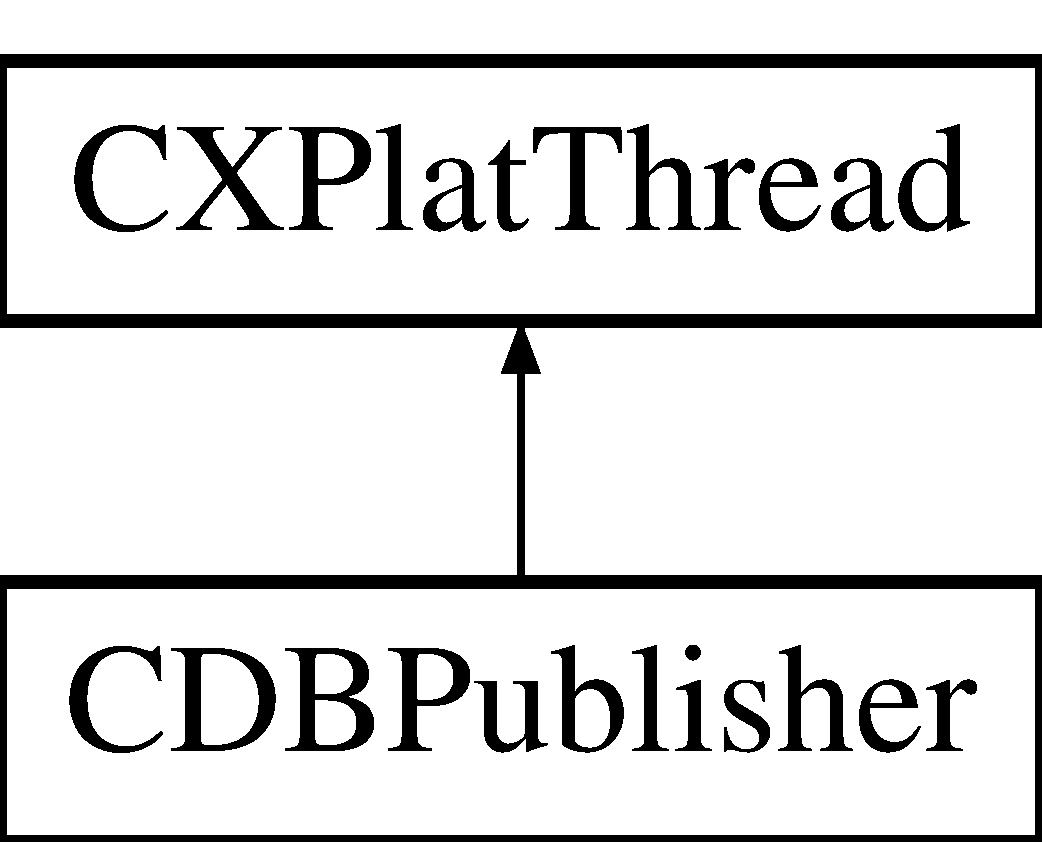
\includegraphics[height=2.000000cm]{class_c_d_b_publisher}
\end{center}
\end{figure}
\subsection*{\-Public \-Member \-Functions}
\begin{DoxyCompactItemize}
\item 
\hyperlink{class_c_d_b_publisher_a9a8efc4caa9c43a26d3cad455c492f4e}{\-C\-D\-B\-Publisher} ()
\item 
virtual \hyperlink{class_c_d_b_publisher_a2d60a06ada8b48aea982b9c57742242a}{$\sim$\-C\-D\-B\-Publisher} ()
\item 
\hyperlink{_cpclient_8h_a6464f7480a0fd0ee170cba12b2c0497f}{void} \hyperlink{class_c_d_b_publisher_a4acf6ea6c628b0387980481a91308d34}{\-Start\-Publishing} (const char $\ast$p\-Database, const char $\ast$p\-Collection, \hyperlink{_c_d_b_publisher_8h_a4663229004d120a06c202e46db5d2d4d}{\-V\-E\-C\-\_\-\-D\-B\-\_\-\-K\-E\-Y\-S} \&\hyperlink{class_c_d_b_publisher_a05607846e2fc5c63010536113ca2534e}{v\-Keys}, const char $\ast$p\-Host, const char $\ast$p\-User, const char $\ast$p\-Password)
\begin{DoxyCompactList}\small\item\em to ensure that the indices exist in the collection. \-Starts publishing thread. \end{DoxyCompactList}\item 
\hyperlink{_cpclient_8h_a6464f7480a0fd0ee170cba12b2c0497f}{void} \hyperlink{class_c_d_b_publisher_abb90cd8717d2e9dbd54773b93656e84d}{\-Stop\-Publishing} ()
\begin{DoxyCompactList}\small\item\em \-Stop publishing. \-Stops the publishing thread. \end{DoxyCompactList}\item 
bool \hyperlink{class_c_d_b_publisher_a8bc747ffa64b62a88b74c760a2a2597c}{\-Publish} (\hyperlink{class_c_d_b_records_array}{\-C\-D\-B\-Records\-Array} \&c\-Records)
\item 
\hyperlink{class_d_b_stats}{\-D\-B\-Stats} \& \hyperlink{class_c_d_b_publisher_a55177dd8e98fae569d4b8c23a79b570e}{\-Get\-D\-B\-Stats} ()
\item 
\hyperlink{_cpclient_8h_a6464f7480a0fd0ee170cba12b2c0497f}{void} \hyperlink{class_c_d_b_publisher_a7591f857cb6edfb1a45e5d27ae1be81b}{\-Set\-Upsert} (bool b\-On\-Off)
\item 
bool \hyperlink{class_c_d_b_publisher_ad9b39dde0e69485ff6ce0ddeb008f127}{\-Get\-Upsert} ()
\begin{DoxyCompactList}\small\item\em \-See if the upsert flag is set. \end{DoxyCompactList}\end{DoxyCompactItemize}
\subsection*{\-Public \-Attributes}
\begin{DoxyCompactItemize}
\item 
time\-\_\-t \hyperlink{class_c_d_b_publisher_a2cf425adefacf57d8ab03b3c77a7de8c}{t\-Last\-Published}
\begin{DoxyCompactList}\small\item\em \-Our last published timestamp. \end{DoxyCompactList}\end{DoxyCompactItemize}
\subsection*{\-Protected \-Member \-Functions}
\begin{DoxyCompactItemize}
\item 
virtual unsigned \hyperlink{class_c_d_b_publisher_afc97488b3517b0d78331b6c54475ab81}{\-Worker\-Function} (\hyperlink{_cpclient_8h_a6464f7480a0fd0ee170cba12b2c0497f}{void} $\ast$p\-Param)
\begin{DoxyCompactList}\small\item\em \-Called by \hyperlink{class_c_x_plat_thread}{\-C\-X\-Plat\-Thread} to start work in object context. \end{DoxyCompactList}\end{DoxyCompactItemize}
\subsection*{\-Protected \-Attributes}
\begin{DoxyCompactItemize}
\item 
\hyperlink{class_d_b_stats}{\-D\-B\-Stats} \hyperlink{class_c_d_b_publisher_a6b1709641e8a184c32ce1776547c43ca}{c\-D\-B\-Stats}
\item 
\hyperlink{class_c_x_plat_critical_section}{\-C\-X\-Plat\-Critical\-Section} \hyperlink{class_c_d_b_publisher_adbf98e64ef485c1d32d758e3935f9746}{c\-Publish\-Mutex}
\item 
\hyperlink{class_c_x_plat_event}{\-C\-X\-Plat\-Event} \hyperlink{class_c_d_b_publisher_a09ae2e573252d271614d487a8db7313f}{c\-Start\-Event}
\item 
string \hyperlink{class_c_d_b_publisher_ab5978dae8e2b51382c7b754b00eb6f37}{s\-Host}
\item 
string \hyperlink{class_c_d_b_publisher_a70c6a70a3eac533267cd6c09d7e4cfe4}{s\-User}
\item 
string \hyperlink{class_c_d_b_publisher_af7857687fa866673f59598535a191139}{s\-Password}
\item 
bool \hyperlink{class_c_d_b_publisher_a067f21d227664a36fcccfba89a03b89c}{b\-Terminate}
\item 
string \hyperlink{class_c_d_b_publisher_ab5f77007ed9fe5e7dae2fc4adf5f3661}{s\-Database}
\item 
\hyperlink{_c_d_b_records_array_8h_a32e3940d41c32d8e161b8775f6c4296a}{\-V\-E\-C\-\_\-\-D\-B\-\_\-\-R\-E\-C\-O\-R\-D\-S} \hyperlink{class_c_d_b_publisher_af3c16b9ccfd3d1df26c1ebf91bd6a987}{v\-D\-B\-Records}
\item 
\hyperlink{_c_d_b_publisher_8h_a4663229004d120a06c202e46db5d2d4d}{\-V\-E\-C\-\_\-\-D\-B\-\_\-\-K\-E\-Y\-S} \hyperlink{class_c_d_b_publisher_a05607846e2fc5c63010536113ca2534e}{v\-Keys}
\item 
string \hyperlink{class_c_d_b_publisher_ac6db2d0df8562fa55c15d7aa5414e285}{s\-Collection}
\item 
string \hyperlink{class_c_d_b_publisher_a10c344b92ca8af51800352cdb99c47c6}{s\-D\-B\-\_\-\-Collection}
\end{DoxyCompactItemize}
\subsection*{\-Static \-Protected \-Attributes}
\begin{DoxyCompactItemize}
\item 
static \hyperlink{class_d_b_stats}{\-D\-B\-Stats} \hyperlink{class_c_d_b_publisher_a3a63670d4729d713995f05fd4a83a2ba}{c\-D\-B\-Copy}
\end{DoxyCompactItemize}


\subsection{\-Detailed \-Description}
\hyperlink{class_c_d_b_publisher}{\-C\-D\-B\-Publisher} -\/ publisher thread \-This class takes a set of records to be published to the \-Mongo\-D\-B and writes them in bulk on a schedule 

\-Definition at line 63 of file \-C\-D\-B\-Publisher.\-h.



\subsection{\-Constructor \& \-Destructor \-Documentation}
\hypertarget{class_c_d_b_publisher_a9a8efc4caa9c43a26d3cad455c492f4e}{\index{\-C\-D\-B\-Publisher@{\-C\-D\-B\-Publisher}!\-C\-D\-B\-Publisher@{\-C\-D\-B\-Publisher}}
\index{\-C\-D\-B\-Publisher@{\-C\-D\-B\-Publisher}!CDBPublisher@{\-C\-D\-B\-Publisher}}
\subsubsection[{\-C\-D\-B\-Publisher}]{\setlength{\rightskip}{0pt plus 5cm}{\bf \-C\-D\-B\-Publisher\-::\-C\-D\-B\-Publisher} (
\begin{DoxyParamCaption}
{}
\end{DoxyParamCaption}
)}}\label{class_c_d_b_publisher_a9a8efc4caa9c43a26d3cad455c492f4e}


\-Definition at line 26 of file \-C\-D\-B\-Publisher.\-cpp.

\hypertarget{class_c_d_b_publisher_a2d60a06ada8b48aea982b9c57742242a}{\index{\-C\-D\-B\-Publisher@{\-C\-D\-B\-Publisher}!$\sim$\-C\-D\-B\-Publisher@{$\sim$\-C\-D\-B\-Publisher}}
\index{$\sim$\-C\-D\-B\-Publisher@{$\sim$\-C\-D\-B\-Publisher}!CDBPublisher@{\-C\-D\-B\-Publisher}}
\subsubsection[{$\sim$\-C\-D\-B\-Publisher}]{\setlength{\rightskip}{0pt plus 5cm}{\bf \-C\-D\-B\-Publisher\-::$\sim$\-C\-D\-B\-Publisher} (
\begin{DoxyParamCaption}
{}
\end{DoxyParamCaption}
)\hspace{0.3cm}{\ttfamily  \mbox{[}virtual\mbox{]}}}}\label{class_c_d_b_publisher_a2d60a06ada8b48aea982b9c57742242a}


\-Definition at line 34 of file \-C\-D\-B\-Publisher.\-cpp.



\subsection{\-Member \-Function \-Documentation}
\hypertarget{class_c_d_b_publisher_a55177dd8e98fae569d4b8c23a79b570e}{\index{\-C\-D\-B\-Publisher@{\-C\-D\-B\-Publisher}!\-Get\-D\-B\-Stats@{\-Get\-D\-B\-Stats}}
\index{\-Get\-D\-B\-Stats@{\-Get\-D\-B\-Stats}!CDBPublisher@{\-C\-D\-B\-Publisher}}
\subsubsection[{\-Get\-D\-B\-Stats}]{\setlength{\rightskip}{0pt plus 5cm}{\bf \-D\-B\-Stats} \& {\bf \-C\-D\-B\-Publisher\-::\-Get\-D\-B\-Stats} (
\begin{DoxyParamCaption}
{}
\end{DoxyParamCaption}
)}}\label{class_c_d_b_publisher_a55177dd8e98fae569d4b8c23a79b570e}
\-Get and clear statistics. \-This returns a call to a static variable, which means the next call changes it. 

\-Definition at line 215 of file \-C\-D\-B\-Publisher.\-cpp.

\hypertarget{class_c_d_b_publisher_ad9b39dde0e69485ff6ce0ddeb008f127}{\index{\-C\-D\-B\-Publisher@{\-C\-D\-B\-Publisher}!\-Get\-Upsert@{\-Get\-Upsert}}
\index{\-Get\-Upsert@{\-Get\-Upsert}!CDBPublisher@{\-C\-D\-B\-Publisher}}
\subsubsection[{\-Get\-Upsert}]{\setlength{\rightskip}{0pt plus 5cm}bool {\bf \-C\-D\-B\-Publisher\-::\-Get\-Upsert} (
\begin{DoxyParamCaption}
{}
\end{DoxyParamCaption}
)}}\label{class_c_d_b_publisher_ad9b39dde0e69485ff6ce0ddeb008f127}


\-See if the upsert flag is set. 



\-Definition at line 76 of file \-C\-D\-B\-Publisher.\-cpp.

\hypertarget{class_c_d_b_publisher_a8bc747ffa64b62a88b74c760a2a2597c}{\index{\-C\-D\-B\-Publisher@{\-C\-D\-B\-Publisher}!\-Publish@{\-Publish}}
\index{\-Publish@{\-Publish}!CDBPublisher@{\-C\-D\-B\-Publisher}}
\subsubsection[{\-Publish}]{\setlength{\rightskip}{0pt plus 5cm}bool {\bf \-C\-D\-B\-Publisher\-::\-Publish} (
\begin{DoxyParamCaption}
\item[{{\bf \-C\-D\-B\-Records\-Array} \&}]{c\-Records}
\end{DoxyParamCaption}
)}}\label{class_c_d_b_publisher_a8bc747ffa64b62a88b74c760a2a2597c}
\-Publish records. \-This will copy the data from the passed in array, clear the array, and return immediately while connecting and writing in the background. 

\-Definition at line 83 of file \-C\-D\-B\-Publisher.\-cpp.

\hypertarget{class_c_d_b_publisher_a7591f857cb6edfb1a45e5d27ae1be81b}{\index{\-C\-D\-B\-Publisher@{\-C\-D\-B\-Publisher}!\-Set\-Upsert@{\-Set\-Upsert}}
\index{\-Set\-Upsert@{\-Set\-Upsert}!CDBPublisher@{\-C\-D\-B\-Publisher}}
\subsubsection[{\-Set\-Upsert}]{\setlength{\rightskip}{0pt plus 5cm}{\bf void} {\bf \-C\-D\-B\-Publisher\-::\-Set\-Upsert} (
\begin{DoxyParamCaption}
\item[{bool}]{b\-On\-Off}
\end{DoxyParamCaption}
)}}\label{class_c_d_b_publisher_a7591f857cb6edfb1a45e5d27ae1be81b}
\-Set upsert. \-Since \-Mongo doesn't have an \char`\"{}upsert\char`\"{} per se, this is a very expensive setting, performance wise. \-It will bulk delete all records before an insert is done. 

\-Definition at line 70 of file \-C\-D\-B\-Publisher.\-cpp.

\hypertarget{class_c_d_b_publisher_a4acf6ea6c628b0387980481a91308d34}{\index{\-C\-D\-B\-Publisher@{\-C\-D\-B\-Publisher}!\-Start\-Publishing@{\-Start\-Publishing}}
\index{\-Start\-Publishing@{\-Start\-Publishing}!CDBPublisher@{\-C\-D\-B\-Publisher}}
\subsubsection[{\-Start\-Publishing}]{\setlength{\rightskip}{0pt plus 5cm}{\bf void} {\bf \-C\-D\-B\-Publisher\-::\-Start\-Publishing} (
\begin{DoxyParamCaption}
\item[{const char $\ast$}]{p\-Database, }
\item[{const char $\ast$}]{p\-Collection, }
\item[{{\bf \-V\-E\-C\-\_\-\-D\-B\-\_\-\-K\-E\-Y\-S} \&}]{v\-Keys, }
\item[{const char $\ast$}]{p\-Host, }
\item[{const char $\ast$}]{p\-User, }
\item[{const char $\ast$}]{p\-Password}
\end{DoxyParamCaption}
)}}\label{class_c_d_b_publisher_a4acf6ea6c628b0387980481a91308d34}


to ensure that the indices exist in the collection. \-Starts publishing thread. 

\-Set \-D\-B config. v\-Keys is an array of index strings (\-J\-S\-O\-N, ex. \char`\"{}\{'node'\-: 1 \}\char`\"{}) 

\-Definition at line 42 of file \-C\-D\-B\-Publisher.\-cpp.

\hypertarget{class_c_d_b_publisher_abb90cd8717d2e9dbd54773b93656e84d}{\index{\-C\-D\-B\-Publisher@{\-C\-D\-B\-Publisher}!\-Stop\-Publishing@{\-Stop\-Publishing}}
\index{\-Stop\-Publishing@{\-Stop\-Publishing}!CDBPublisher@{\-C\-D\-B\-Publisher}}
\subsubsection[{\-Stop\-Publishing}]{\setlength{\rightskip}{0pt plus 5cm}{\bf void} {\bf \-C\-D\-B\-Publisher\-::\-Stop\-Publishing} (
\begin{DoxyParamCaption}
{}
\end{DoxyParamCaption}
)}}\label{class_c_d_b_publisher_abb90cd8717d2e9dbd54773b93656e84d}


\-Stop publishing. \-Stops the publishing thread. 



\-Definition at line 60 of file \-C\-D\-B\-Publisher.\-cpp.

\hypertarget{class_c_d_b_publisher_afc97488b3517b0d78331b6c54475ab81}{\index{\-C\-D\-B\-Publisher@{\-C\-D\-B\-Publisher}!\-Worker\-Function@{\-Worker\-Function}}
\index{\-Worker\-Function@{\-Worker\-Function}!CDBPublisher@{\-C\-D\-B\-Publisher}}
\subsubsection[{\-Worker\-Function}]{\setlength{\rightskip}{0pt plus 5cm}unsigned {\bf \-C\-D\-B\-Publisher\-::\-Worker\-Function} (
\begin{DoxyParamCaption}
\item[{{\bf void} $\ast$}]{p\-Param}
\end{DoxyParamCaption}
)\hspace{0.3cm}{\ttfamily  \mbox{[}protected, virtual\mbox{]}}}}\label{class_c_d_b_publisher_afc97488b3517b0d78331b6c54475ab81}


\-Called by \hyperlink{class_c_x_plat_thread}{\-C\-X\-Plat\-Thread} to start work in object context. 



\-Implements \hyperlink{class_c_x_plat_thread_af8a15900817f9673c6fd8e85cdedf27d}{\-C\-X\-Plat\-Thread}.



\-Definition at line 113 of file \-C\-D\-B\-Publisher.\-cpp.



\subsection{\-Member \-Data \-Documentation}
\hypertarget{class_c_d_b_publisher_a067f21d227664a36fcccfba89a03b89c}{\index{\-C\-D\-B\-Publisher@{\-C\-D\-B\-Publisher}!b\-Terminate@{b\-Terminate}}
\index{b\-Terminate@{b\-Terminate}!CDBPublisher@{\-C\-D\-B\-Publisher}}
\subsubsection[{b\-Terminate}]{\setlength{\rightskip}{0pt plus 5cm}bool {\bf \-C\-D\-B\-Publisher\-::b\-Terminate}\hspace{0.3cm}{\ttfamily  \mbox{[}protected\mbox{]}}}}\label{class_c_d_b_publisher_a067f21d227664a36fcccfba89a03b89c}


\-Definition at line 102 of file \-C\-D\-B\-Publisher.\-h.

\hypertarget{class_c_d_b_publisher_a3a63670d4729d713995f05fd4a83a2ba}{\index{\-C\-D\-B\-Publisher@{\-C\-D\-B\-Publisher}!c\-D\-B\-Copy@{c\-D\-B\-Copy}}
\index{c\-D\-B\-Copy@{c\-D\-B\-Copy}!CDBPublisher@{\-C\-D\-B\-Publisher}}
\subsubsection[{c\-D\-B\-Copy}]{\setlength{\rightskip}{0pt plus 5cm}{\bf \-D\-B\-Stats} {\bf \-C\-D\-B\-Publisher\-::c\-D\-B\-Copy}\hspace{0.3cm}{\ttfamily  \mbox{[}static, protected\mbox{]}}}}\label{class_c_d_b_publisher_a3a63670d4729d713995f05fd4a83a2ba}


\-Definition at line 96 of file \-C\-D\-B\-Publisher.\-h.

\hypertarget{class_c_d_b_publisher_a6b1709641e8a184c32ce1776547c43ca}{\index{\-C\-D\-B\-Publisher@{\-C\-D\-B\-Publisher}!c\-D\-B\-Stats@{c\-D\-B\-Stats}}
\index{c\-D\-B\-Stats@{c\-D\-B\-Stats}!CDBPublisher@{\-C\-D\-B\-Publisher}}
\subsubsection[{c\-D\-B\-Stats}]{\setlength{\rightskip}{0pt plus 5cm}{\bf \-D\-B\-Stats} {\bf \-C\-D\-B\-Publisher\-::c\-D\-B\-Stats}\hspace{0.3cm}{\ttfamily  \mbox{[}protected\mbox{]}}}}\label{class_c_d_b_publisher_a6b1709641e8a184c32ce1776547c43ca}


\-Definition at line 95 of file \-C\-D\-B\-Publisher.\-h.

\hypertarget{class_c_d_b_publisher_adbf98e64ef485c1d32d758e3935f9746}{\index{\-C\-D\-B\-Publisher@{\-C\-D\-B\-Publisher}!c\-Publish\-Mutex@{c\-Publish\-Mutex}}
\index{c\-Publish\-Mutex@{c\-Publish\-Mutex}!CDBPublisher@{\-C\-D\-B\-Publisher}}
\subsubsection[{c\-Publish\-Mutex}]{\setlength{\rightskip}{0pt plus 5cm}{\bf \-C\-X\-Plat\-Critical\-Section} {\bf \-C\-D\-B\-Publisher\-::c\-Publish\-Mutex}\hspace{0.3cm}{\ttfamily  \mbox{[}protected\mbox{]}}}}\label{class_c_d_b_publisher_adbf98e64ef485c1d32d758e3935f9746}


\-Definition at line 97 of file \-C\-D\-B\-Publisher.\-h.

\hypertarget{class_c_d_b_publisher_a09ae2e573252d271614d487a8db7313f}{\index{\-C\-D\-B\-Publisher@{\-C\-D\-B\-Publisher}!c\-Start\-Event@{c\-Start\-Event}}
\index{c\-Start\-Event@{c\-Start\-Event}!CDBPublisher@{\-C\-D\-B\-Publisher}}
\subsubsection[{c\-Start\-Event}]{\setlength{\rightskip}{0pt plus 5cm}{\bf \-C\-X\-Plat\-Event} {\bf \-C\-D\-B\-Publisher\-::c\-Start\-Event}\hspace{0.3cm}{\ttfamily  \mbox{[}protected\mbox{]}}}}\label{class_c_d_b_publisher_a09ae2e573252d271614d487a8db7313f}


\-Definition at line 98 of file \-C\-D\-B\-Publisher.\-h.

\hypertarget{class_c_d_b_publisher_ac6db2d0df8562fa55c15d7aa5414e285}{\index{\-C\-D\-B\-Publisher@{\-C\-D\-B\-Publisher}!s\-Collection@{s\-Collection}}
\index{s\-Collection@{s\-Collection}!CDBPublisher@{\-C\-D\-B\-Publisher}}
\subsubsection[{s\-Collection}]{\setlength{\rightskip}{0pt plus 5cm}string {\bf \-C\-D\-B\-Publisher\-::s\-Collection}\hspace{0.3cm}{\ttfamily  \mbox{[}protected\mbox{]}}}}\label{class_c_d_b_publisher_ac6db2d0df8562fa55c15d7aa5414e285}


\-Definition at line 106 of file \-C\-D\-B\-Publisher.\-h.

\hypertarget{class_c_d_b_publisher_ab5f77007ed9fe5e7dae2fc4adf5f3661}{\index{\-C\-D\-B\-Publisher@{\-C\-D\-B\-Publisher}!s\-Database@{s\-Database}}
\index{s\-Database@{s\-Database}!CDBPublisher@{\-C\-D\-B\-Publisher}}
\subsubsection[{s\-Database}]{\setlength{\rightskip}{0pt plus 5cm}string {\bf \-C\-D\-B\-Publisher\-::s\-Database}\hspace{0.3cm}{\ttfamily  \mbox{[}protected\mbox{]}}}}\label{class_c_d_b_publisher_ab5f77007ed9fe5e7dae2fc4adf5f3661}


\-Definition at line 103 of file \-C\-D\-B\-Publisher.\-h.

\hypertarget{class_c_d_b_publisher_a10c344b92ca8af51800352cdb99c47c6}{\index{\-C\-D\-B\-Publisher@{\-C\-D\-B\-Publisher}!s\-D\-B\-\_\-\-Collection@{s\-D\-B\-\_\-\-Collection}}
\index{s\-D\-B\-\_\-\-Collection@{s\-D\-B\-\_\-\-Collection}!CDBPublisher@{\-C\-D\-B\-Publisher}}
\subsubsection[{s\-D\-B\-\_\-\-Collection}]{\setlength{\rightskip}{0pt plus 5cm}string {\bf \-C\-D\-B\-Publisher\-::s\-D\-B\-\_\-\-Collection}\hspace{0.3cm}{\ttfamily  \mbox{[}protected\mbox{]}}}}\label{class_c_d_b_publisher_a10c344b92ca8af51800352cdb99c47c6}


\-Definition at line 107 of file \-C\-D\-B\-Publisher.\-h.

\hypertarget{class_c_d_b_publisher_ab5978dae8e2b51382c7b754b00eb6f37}{\index{\-C\-D\-B\-Publisher@{\-C\-D\-B\-Publisher}!s\-Host@{s\-Host}}
\index{s\-Host@{s\-Host}!CDBPublisher@{\-C\-D\-B\-Publisher}}
\subsubsection[{s\-Host}]{\setlength{\rightskip}{0pt plus 5cm}string {\bf \-C\-D\-B\-Publisher\-::s\-Host}\hspace{0.3cm}{\ttfamily  \mbox{[}protected\mbox{]}}}}\label{class_c_d_b_publisher_ab5978dae8e2b51382c7b754b00eb6f37}


\-Definition at line 99 of file \-C\-D\-B\-Publisher.\-h.

\hypertarget{class_c_d_b_publisher_af7857687fa866673f59598535a191139}{\index{\-C\-D\-B\-Publisher@{\-C\-D\-B\-Publisher}!s\-Password@{s\-Password}}
\index{s\-Password@{s\-Password}!CDBPublisher@{\-C\-D\-B\-Publisher}}
\subsubsection[{s\-Password}]{\setlength{\rightskip}{0pt plus 5cm}string {\bf \-C\-D\-B\-Publisher\-::s\-Password}\hspace{0.3cm}{\ttfamily  \mbox{[}protected\mbox{]}}}}\label{class_c_d_b_publisher_af7857687fa866673f59598535a191139}


\-Definition at line 101 of file \-C\-D\-B\-Publisher.\-h.

\hypertarget{class_c_d_b_publisher_a70c6a70a3eac533267cd6c09d7e4cfe4}{\index{\-C\-D\-B\-Publisher@{\-C\-D\-B\-Publisher}!s\-User@{s\-User}}
\index{s\-User@{s\-User}!CDBPublisher@{\-C\-D\-B\-Publisher}}
\subsubsection[{s\-User}]{\setlength{\rightskip}{0pt plus 5cm}string {\bf \-C\-D\-B\-Publisher\-::s\-User}\hspace{0.3cm}{\ttfamily  \mbox{[}protected\mbox{]}}}}\label{class_c_d_b_publisher_a70c6a70a3eac533267cd6c09d7e4cfe4}


\-Definition at line 100 of file \-C\-D\-B\-Publisher.\-h.

\hypertarget{class_c_d_b_publisher_a2cf425adefacf57d8ab03b3c77a7de8c}{\index{\-C\-D\-B\-Publisher@{\-C\-D\-B\-Publisher}!t\-Last\-Published@{t\-Last\-Published}}
\index{t\-Last\-Published@{t\-Last\-Published}!CDBPublisher@{\-C\-D\-B\-Publisher}}
\subsubsection[{t\-Last\-Published}]{\setlength{\rightskip}{0pt plus 5cm}time\-\_\-t {\bf \-C\-D\-B\-Publisher\-::t\-Last\-Published}}}\label{class_c_d_b_publisher_a2cf425adefacf57d8ab03b3c77a7de8c}


\-Our last published timestamp. 



\-Definition at line 89 of file \-C\-D\-B\-Publisher.\-h.

\hypertarget{class_c_d_b_publisher_af3c16b9ccfd3d1df26c1ebf91bd6a987}{\index{\-C\-D\-B\-Publisher@{\-C\-D\-B\-Publisher}!v\-D\-B\-Records@{v\-D\-B\-Records}}
\index{v\-D\-B\-Records@{v\-D\-B\-Records}!CDBPublisher@{\-C\-D\-B\-Publisher}}
\subsubsection[{v\-D\-B\-Records}]{\setlength{\rightskip}{0pt plus 5cm}{\bf \-V\-E\-C\-\_\-\-D\-B\-\_\-\-R\-E\-C\-O\-R\-D\-S} {\bf \-C\-D\-B\-Publisher\-::v\-D\-B\-Records}\hspace{0.3cm}{\ttfamily  \mbox{[}protected\mbox{]}}}}\label{class_c_d_b_publisher_af3c16b9ccfd3d1df26c1ebf91bd6a987}


\-Definition at line 104 of file \-C\-D\-B\-Publisher.\-h.

\hypertarget{class_c_d_b_publisher_a05607846e2fc5c63010536113ca2534e}{\index{\-C\-D\-B\-Publisher@{\-C\-D\-B\-Publisher}!v\-Keys@{v\-Keys}}
\index{v\-Keys@{v\-Keys}!CDBPublisher@{\-C\-D\-B\-Publisher}}
\subsubsection[{v\-Keys}]{\setlength{\rightskip}{0pt plus 5cm}{\bf \-V\-E\-C\-\_\-\-D\-B\-\_\-\-K\-E\-Y\-S} {\bf \-C\-D\-B\-Publisher\-::v\-Keys}\hspace{0.3cm}{\ttfamily  \mbox{[}protected\mbox{]}}}}\label{class_c_d_b_publisher_a05607846e2fc5c63010536113ca2534e}


\-Definition at line 105 of file \-C\-D\-B\-Publisher.\-h.



\-The documentation for this class was generated from the following files\-:\begin{DoxyCompactItemize}
\item 
common/\hyperlink{_c_d_b_publisher_8h}{\-C\-D\-B\-Publisher.\-h}\item 
common/\hyperlink{_c_d_b_publisher_8cpp}{\-C\-D\-B\-Publisher.\-cpp}\end{DoxyCompactItemize}

\hypertarget{class_c_d_b_records_array}{\section{\-C\-D\-B\-Records\-Array \-Class \-Reference}
\label{class_c_d_b_records_array}\index{\-C\-D\-B\-Records\-Array@{\-C\-D\-B\-Records\-Array}}
}


{\ttfamily \#include $<$\-C\-D\-B\-Records\-Array.\-h$>$}

\subsection*{\-Public \-Member \-Functions}
\begin{DoxyCompactItemize}
\item 
\hyperlink{class_c_d_b_records_array_a1a34c7690fc2d0f4eff418a39c0d0985}{\-C\-D\-B\-Records\-Array} ()
\item 
\hyperlink{class_c_d_b_records_array_a2956116f14e5fa19a6386ffd23053c4d}{\-C\-D\-B\-Records\-Array} (const \hyperlink{class_c_d_b_records_array}{\-C\-D\-B\-Records\-Array} \&orig)
\item 
virtual \hyperlink{class_c_d_b_records_array_a9b9b7ecd895df030784764291f57537d}{$\sim$\-C\-D\-B\-Records\-Array} ()
\item 
\hyperlink{_cpclient_8h_a6464f7480a0fd0ee170cba12b2c0497f}{void} \hyperlink{class_c_d_b_records_array_ae71da68787e56a916aa4149abd6912b1}{\-D\-B\-Record\-Add} (const char $\ast$p\-Record, float f\-Elapsed=0.\-0f)
\begin{DoxyCompactList}\small\item\em \-Add a record to the \-D\-B record array.. \-Synchronized with the publisher. \end{DoxyCompactList}\item 
\hyperlink{_cpclient_8h_a6464f7480a0fd0ee170cba12b2c0497f}{void} \hyperlink{class_c_d_b_records_array_a7442b3cefd55b855f6128331b87d1bc5}{\-D\-B\-Record\-Add} (\hyperlink{_c_d_b_records_array_8h_a32e3940d41c32d8e161b8775f6c4296a}{\-V\-E\-C\-\_\-\-D\-B\-\_\-\-R\-E\-C\-O\-R\-D\-S} \&v\-Rec, float f\-Elapsed=0.\-0f)
\begin{DoxyCompactList}\small\item\em \-Add a whole array of records. \end{DoxyCompactList}\item 
\hyperlink{_c_d_b_records_array_8h_a32e3940d41c32d8e161b8775f6c4296a}{\-V\-E\-C\-\_\-\-D\-B\-\_\-\-R\-E\-C\-O\-R\-D\-S} $\ast$ \hyperlink{class_c_d_b_records_array_a04a84400f1419abd3dca2cb3834f7071}{\-Lock\-D\-B\-Records} ()
\begin{DoxyCompactList}\small\item\em \-Get \-D\-B record array -\/ locks the array. \end{DoxyCompactList}\item 
bool \hyperlink{class_c_d_b_records_array_a421c6732b6d17ea3080ad19c3c250478}{\-Clear\-D\-B\-Records} ()
\begin{DoxyCompactList}\small\item\em \-Clear the array. \end{DoxyCompactList}\item 
\hyperlink{_cpclient_8h_a6464f7480a0fd0ee170cba12b2c0497f}{void} \hyperlink{class_c_d_b_records_array_aeb1530f115743efe2f2d231dcc555ced}{\-Unlock\-D\-B\-Records} ()
\begin{DoxyCompactList}\small\item\em \-Release \-D\-B record array -\/ must be called after \char`\"{}\-Get\-Record\-Array\char`\"{}. \end{DoxyCompactList}\end{DoxyCompactItemize}
\subsection*{\-Public \-Attributes}
\begin{DoxyCompactItemize}
\item 
\hyperlink{_c_d_b_records_array_8h_a32e3940d41c32d8e161b8775f6c4296a}{\-V\-E\-C\-\_\-\-D\-B\-\_\-\-R\-E\-C\-O\-R\-D\-S} \hyperlink{class_c_d_b_records_array_a5f29315f1b26188a7b53790b4d65dfda}{v\-D\-B\-Records}
\begin{DoxyCompactList}\small\item\em \-Array of the records. \end{DoxyCompactList}\item 
float \hyperlink{class_c_d_b_records_array_aa64819ed7441e3e28fc6cf13e42713d0}{f\-Total\-Elapsed}
\begin{DoxyCompactList}\small\item\em \-Total elapsed time to publish the records. \end{DoxyCompactList}\end{DoxyCompactItemize}


\subsection{\-Detailed \-Description}
\hyperlink{class_c_d_b_records_array}{\-C\-D\-B\-Records\-Array} \-Class to encapsulate the records that we want to publish to \-Mongo 

\-Definition at line 32 of file \-C\-D\-B\-Records\-Array.\-h.



\subsection{\-Constructor \& \-Destructor \-Documentation}
\hypertarget{class_c_d_b_records_array_a1a34c7690fc2d0f4eff418a39c0d0985}{\index{\-C\-D\-B\-Records\-Array@{\-C\-D\-B\-Records\-Array}!\-C\-D\-B\-Records\-Array@{\-C\-D\-B\-Records\-Array}}
\index{\-C\-D\-B\-Records\-Array@{\-C\-D\-B\-Records\-Array}!CDBRecordsArray@{\-C\-D\-B\-Records\-Array}}
\subsubsection[{\-C\-D\-B\-Records\-Array}]{\setlength{\rightskip}{0pt plus 5cm}{\bf \-C\-D\-B\-Records\-Array\-::\-C\-D\-B\-Records\-Array} (
\begin{DoxyParamCaption}
{}
\end{DoxyParamCaption}
)}}\label{class_c_d_b_records_array_a1a34c7690fc2d0f4eff418a39c0d0985}


\-Definition at line 18 of file \-C\-D\-B\-Records\-Array.\-cpp.

\hypertarget{class_c_d_b_records_array_a2956116f14e5fa19a6386ffd23053c4d}{\index{\-C\-D\-B\-Records\-Array@{\-C\-D\-B\-Records\-Array}!\-C\-D\-B\-Records\-Array@{\-C\-D\-B\-Records\-Array}}
\index{\-C\-D\-B\-Records\-Array@{\-C\-D\-B\-Records\-Array}!CDBRecordsArray@{\-C\-D\-B\-Records\-Array}}
\subsubsection[{\-C\-D\-B\-Records\-Array}]{\setlength{\rightskip}{0pt plus 5cm}{\bf \-C\-D\-B\-Records\-Array\-::\-C\-D\-B\-Records\-Array} (
\begin{DoxyParamCaption}
\item[{const {\bf \-C\-D\-B\-Records\-Array} \&}]{orig}
\end{DoxyParamCaption}
)}}\label{class_c_d_b_records_array_a2956116f14e5fa19a6386ffd23053c4d}


\-Definition at line 24 of file \-C\-D\-B\-Records\-Array.\-cpp.

\hypertarget{class_c_d_b_records_array_a9b9b7ecd895df030784764291f57537d}{\index{\-C\-D\-B\-Records\-Array@{\-C\-D\-B\-Records\-Array}!$\sim$\-C\-D\-B\-Records\-Array@{$\sim$\-C\-D\-B\-Records\-Array}}
\index{$\sim$\-C\-D\-B\-Records\-Array@{$\sim$\-C\-D\-B\-Records\-Array}!CDBRecordsArray@{\-C\-D\-B\-Records\-Array}}
\subsubsection[{$\sim$\-C\-D\-B\-Records\-Array}]{\setlength{\rightskip}{0pt plus 5cm}{\bf \-C\-D\-B\-Records\-Array\-::$\sim$\-C\-D\-B\-Records\-Array} (
\begin{DoxyParamCaption}
{}
\end{DoxyParamCaption}
)\hspace{0.3cm}{\ttfamily  \mbox{[}virtual\mbox{]}}}}\label{class_c_d_b_records_array_a9b9b7ecd895df030784764291f57537d}


\-Definition at line 32 of file \-C\-D\-B\-Records\-Array.\-cpp.



\subsection{\-Member \-Function \-Documentation}
\hypertarget{class_c_d_b_records_array_a421c6732b6d17ea3080ad19c3c250478}{\index{\-C\-D\-B\-Records\-Array@{\-C\-D\-B\-Records\-Array}!\-Clear\-D\-B\-Records@{\-Clear\-D\-B\-Records}}
\index{\-Clear\-D\-B\-Records@{\-Clear\-D\-B\-Records}!CDBRecordsArray@{\-C\-D\-B\-Records\-Array}}
\subsubsection[{\-Clear\-D\-B\-Records}]{\setlength{\rightskip}{0pt plus 5cm}bool {\bf \-C\-D\-B\-Records\-Array\-::\-Clear\-D\-B\-Records} (
\begin{DoxyParamCaption}
{}
\end{DoxyParamCaption}
)}}\label{class_c_d_b_records_array_a421c6732b6d17ea3080ad19c3c250478}


\-Clear the array. 



\-Definition at line 76 of file \-C\-D\-B\-Records\-Array.\-cpp.

\hypertarget{class_c_d_b_records_array_ae71da68787e56a916aa4149abd6912b1}{\index{\-C\-D\-B\-Records\-Array@{\-C\-D\-B\-Records\-Array}!\-D\-B\-Record\-Add@{\-D\-B\-Record\-Add}}
\index{\-D\-B\-Record\-Add@{\-D\-B\-Record\-Add}!CDBRecordsArray@{\-C\-D\-B\-Records\-Array}}
\subsubsection[{\-D\-B\-Record\-Add}]{\setlength{\rightskip}{0pt plus 5cm}{\bf void} {\bf \-C\-D\-B\-Records\-Array\-::\-D\-B\-Record\-Add} (
\begin{DoxyParamCaption}
\item[{const char $\ast$}]{p\-Record, }
\item[{float}]{f\-Elapsed = {\ttfamily 0.0f}}
\end{DoxyParamCaption}
)}}\label{class_c_d_b_records_array_ae71da68787e56a916aa4149abd6912b1}


\-Add a record to the \-D\-B record array.. \-Synchronized with the publisher. 



\-Definition at line 39 of file \-C\-D\-B\-Records\-Array.\-cpp.

\hypertarget{class_c_d_b_records_array_a7442b3cefd55b855f6128331b87d1bc5}{\index{\-C\-D\-B\-Records\-Array@{\-C\-D\-B\-Records\-Array}!\-D\-B\-Record\-Add@{\-D\-B\-Record\-Add}}
\index{\-D\-B\-Record\-Add@{\-D\-B\-Record\-Add}!CDBRecordsArray@{\-C\-D\-B\-Records\-Array}}
\subsubsection[{\-D\-B\-Record\-Add}]{\setlength{\rightskip}{0pt plus 5cm}{\bf void} {\bf \-C\-D\-B\-Records\-Array\-::\-D\-B\-Record\-Add} (
\begin{DoxyParamCaption}
\item[{{\bf \-V\-E\-C\-\_\-\-D\-B\-\_\-\-R\-E\-C\-O\-R\-D\-S} \&}]{v\-Rec, }
\item[{float}]{f\-Elapsed = {\ttfamily 0.0f}}
\end{DoxyParamCaption}
)}}\label{class_c_d_b_records_array_a7442b3cefd55b855f6128331b87d1bc5}


\-Add a whole array of records. 



\-Definition at line 48 of file \-C\-D\-B\-Records\-Array.\-cpp.

\hypertarget{class_c_d_b_records_array_a04a84400f1419abd3dca2cb3834f7071}{\index{\-C\-D\-B\-Records\-Array@{\-C\-D\-B\-Records\-Array}!\-Lock\-D\-B\-Records@{\-Lock\-D\-B\-Records}}
\index{\-Lock\-D\-B\-Records@{\-Lock\-D\-B\-Records}!CDBRecordsArray@{\-C\-D\-B\-Records\-Array}}
\subsubsection[{\-Lock\-D\-B\-Records}]{\setlength{\rightskip}{0pt plus 5cm}{\bf \-V\-E\-C\-\_\-\-D\-B\-\_\-\-R\-E\-C\-O\-R\-D\-S} $\ast$ {\bf \-C\-D\-B\-Records\-Array\-::\-Lock\-D\-B\-Records} (
\begin{DoxyParamCaption}
{}
\end{DoxyParamCaption}
)}}\label{class_c_d_b_records_array_a04a84400f1419abd3dca2cb3834f7071}


\-Get \-D\-B record array -\/ locks the array. 



\-Definition at line 58 of file \-C\-D\-B\-Records\-Array.\-cpp.

\hypertarget{class_c_d_b_records_array_aeb1530f115743efe2f2d231dcc555ced}{\index{\-C\-D\-B\-Records\-Array@{\-C\-D\-B\-Records\-Array}!\-Unlock\-D\-B\-Records@{\-Unlock\-D\-B\-Records}}
\index{\-Unlock\-D\-B\-Records@{\-Unlock\-D\-B\-Records}!CDBRecordsArray@{\-C\-D\-B\-Records\-Array}}
\subsubsection[{\-Unlock\-D\-B\-Records}]{\setlength{\rightskip}{0pt plus 5cm}{\bf void} {\bf \-C\-D\-B\-Records\-Array\-::\-Unlock\-D\-B\-Records} (
\begin{DoxyParamCaption}
{}
\end{DoxyParamCaption}
)}}\label{class_c_d_b_records_array_aeb1530f115743efe2f2d231dcc555ced}


\-Release \-D\-B record array -\/ must be called after \char`\"{}\-Get\-Record\-Array\char`\"{}. 



\-Definition at line 69 of file \-C\-D\-B\-Records\-Array.\-cpp.



\subsection{\-Member \-Data \-Documentation}
\hypertarget{class_c_d_b_records_array_aa64819ed7441e3e28fc6cf13e42713d0}{\index{\-C\-D\-B\-Records\-Array@{\-C\-D\-B\-Records\-Array}!f\-Total\-Elapsed@{f\-Total\-Elapsed}}
\index{f\-Total\-Elapsed@{f\-Total\-Elapsed}!CDBRecordsArray@{\-C\-D\-B\-Records\-Array}}
\subsubsection[{f\-Total\-Elapsed}]{\setlength{\rightskip}{0pt plus 5cm}float {\bf \-C\-D\-B\-Records\-Array\-::f\-Total\-Elapsed}}}\label{class_c_d_b_records_array_aa64819ed7441e3e28fc6cf13e42713d0}


\-Total elapsed time to publish the records. 



\-Definition at line 54 of file \-C\-D\-B\-Records\-Array.\-h.

\hypertarget{class_c_d_b_records_array_a5f29315f1b26188a7b53790b4d65dfda}{\index{\-C\-D\-B\-Records\-Array@{\-C\-D\-B\-Records\-Array}!v\-D\-B\-Records@{v\-D\-B\-Records}}
\index{v\-D\-B\-Records@{v\-D\-B\-Records}!CDBRecordsArray@{\-C\-D\-B\-Records\-Array}}
\subsubsection[{v\-D\-B\-Records}]{\setlength{\rightskip}{0pt plus 5cm}{\bf \-V\-E\-C\-\_\-\-D\-B\-\_\-\-R\-E\-C\-O\-R\-D\-S} {\bf \-C\-D\-B\-Records\-Array\-::v\-D\-B\-Records}}}\label{class_c_d_b_records_array_a5f29315f1b26188a7b53790b4d65dfda}


\-Array of the records. 



\-Definition at line 52 of file \-C\-D\-B\-Records\-Array.\-h.



\-The documentation for this class was generated from the following files\-:\begin{DoxyCompactItemize}
\item 
common/\hyperlink{_c_d_b_records_array_8h}{\-C\-D\-B\-Records\-Array.\-h}\item 
common/\hyperlink{_c_d_b_records_array_8cpp}{\-C\-D\-B\-Records\-Array.\-cpp}\end{DoxyCompactItemize}

\hypertarget{class_c_echo_client}{\section{\-C\-Echo\-Client \-Class \-Reference}
\label{class_c_echo_client}\index{\-C\-Echo\-Client@{\-C\-Echo\-Client}}
}


{\ttfamily \#include $<$\-C\-Echo\-Client.\-h$>$}

\-Inheritance diagram for \-C\-Echo\-Client\-:\begin{figure}[H]
\begin{center}
\leavevmode
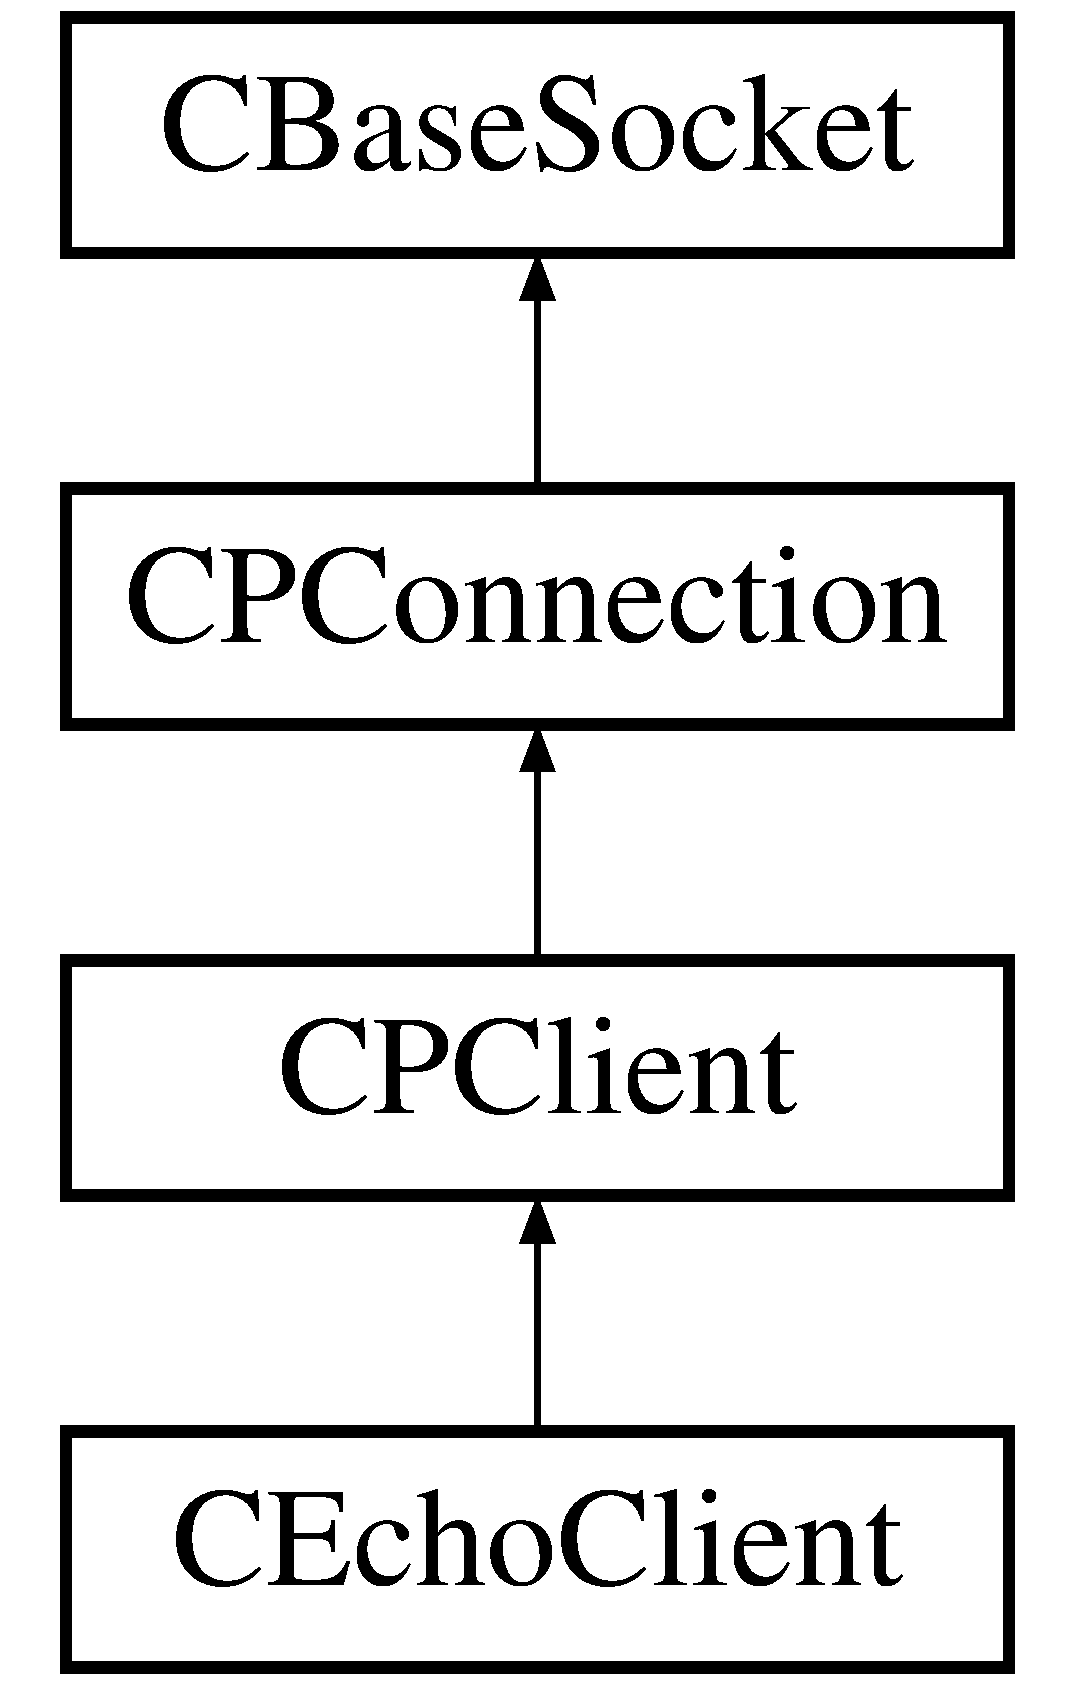
\includegraphics[height=4.000000cm]{class_c_echo_client}
\end{center}
\end{figure}
\subsection*{\-Public \-Member \-Functions}
\begin{DoxyCompactItemize}
\item 
\hyperlink{class_c_echo_client_afb1b50347cc6200df185a1696b88ef57}{\-C\-Echo\-Client} (\hyperlink{_c_p_connection_handler_8h_a05bf2fef946dbf14350a5f45bb28f953}{\-C\-P\-\_\-\-C\-O\-N\-N\-E\-C\-T\-I\-O\-N\-\_\-\-H\-A\-N\-D\-L\-E\-R\-\_\-\-A\-R\-R\-A\-Y} \&c\-P\-C\-Handlers, \hyperlink{_c_p_client_handler_8h_a9babc356867a188aa505ce2ce4a81c46}{\-C\-P\-\_\-\-C\-L\-I\-E\-N\-T\-\_\-\-H\-A\-N\-D\-L\-E\-R\-\_\-\-A\-R\-R\-A\-Y} \&c\-P\-Client\-Handlers)
\item 
virtual \hyperlink{class_c_echo_client_a96ca31a53e72940a5aa33905853182d3}{$\sim$\-C\-Echo\-Client} ()
\item 
\hyperlink{_cpclient_8h_a6464f7480a0fd0ee170cba12b2c0497f}{void} \hyperlink{class_c_echo_client_ad25eb3f1a3cbb2e25fd65b20a5f505ce}{\-Send\-String} (char $\ast$p\-String)
\end{DoxyCompactItemize}
\subsection*{\-Protected \-Member \-Functions}
\begin{DoxyCompactItemize}
\item 
\hyperlink{_cpclient_8h_a3be13892ae7076009afcf121347dd319}{\-B\-O\-O\-L} \hyperlink{class_c_echo_client_aa4b137b9fab962746d02b70a94a400a8}{\-Process\-Data} (unsigned char $\ast$lp\-Data, int i\-Len)
\begin{DoxyCompactList}\small\item\em \-Pure virtual function to process data. \end{DoxyCompactList}\end{DoxyCompactItemize}
\subsection*{\-Protected \-Attributes}
\begin{DoxyCompactItemize}
\item 
char \hyperlink{class_c_echo_client_a59d25bf6a4e77c56bbbde61efb795c42}{sz\-Buf} \mbox{[}4096\mbox{]}
\end{DoxyCompactItemize}


\subsection{\-Detailed \-Description}


\-Definition at line 14 of file \-C\-Echo\-Client.\-h.



\subsection{\-Constructor \& \-Destructor \-Documentation}
\hypertarget{class_c_echo_client_afb1b50347cc6200df185a1696b88ef57}{\index{\-C\-Echo\-Client@{\-C\-Echo\-Client}!\-C\-Echo\-Client@{\-C\-Echo\-Client}}
\index{\-C\-Echo\-Client@{\-C\-Echo\-Client}!CEchoClient@{\-C\-Echo\-Client}}
\subsubsection[{\-C\-Echo\-Client}]{\setlength{\rightskip}{0pt plus 5cm}{\bf \-C\-Echo\-Client\-::\-C\-Echo\-Client} (
\begin{DoxyParamCaption}
\item[{{\bf \-C\-P\-\_\-\-C\-O\-N\-N\-E\-C\-T\-I\-O\-N\-\_\-\-H\-A\-N\-D\-L\-E\-R\-\_\-\-A\-R\-R\-A\-Y} \&}]{c\-P\-C\-Handlers, }
\item[{{\bf \-C\-P\-\_\-\-C\-L\-I\-E\-N\-T\-\_\-\-H\-A\-N\-D\-L\-E\-R\-\_\-\-A\-R\-R\-A\-Y} \&}]{c\-P\-Client\-Handlers}
\end{DoxyParamCaption}
)}}\label{class_c_echo_client_afb1b50347cc6200df185a1696b88ef57}


\-Definition at line 12 of file \-C\-Echo\-Client.\-cpp.

\hypertarget{class_c_echo_client_a96ca31a53e72940a5aa33905853182d3}{\index{\-C\-Echo\-Client@{\-C\-Echo\-Client}!$\sim$\-C\-Echo\-Client@{$\sim$\-C\-Echo\-Client}}
\index{$\sim$\-C\-Echo\-Client@{$\sim$\-C\-Echo\-Client}!CEchoClient@{\-C\-Echo\-Client}}
\subsubsection[{$\sim$\-C\-Echo\-Client}]{\setlength{\rightskip}{0pt plus 5cm}{\bf \-C\-Echo\-Client\-::$\sim$\-C\-Echo\-Client} (
\begin{DoxyParamCaption}
{}
\end{DoxyParamCaption}
)\hspace{0.3cm}{\ttfamily  \mbox{[}virtual\mbox{]}}}}\label{class_c_echo_client_a96ca31a53e72940a5aa33905853182d3}


\-Definition at line 17 of file \-C\-Echo\-Client.\-cpp.



\subsection{\-Member \-Function \-Documentation}
\hypertarget{class_c_echo_client_aa4b137b9fab962746d02b70a94a400a8}{\index{\-C\-Echo\-Client@{\-C\-Echo\-Client}!\-Process\-Data@{\-Process\-Data}}
\index{\-Process\-Data@{\-Process\-Data}!CEchoClient@{\-C\-Echo\-Client}}
\subsubsection[{\-Process\-Data}]{\setlength{\rightskip}{0pt plus 5cm}{\bf \-B\-O\-O\-L} {\bf \-C\-Echo\-Client\-::\-Process\-Data} (
\begin{DoxyParamCaption}
\item[{unsigned char $\ast$}]{lp\-Data, }
\item[{int}]{i\-Len}
\end{DoxyParamCaption}
)\hspace{0.3cm}{\ttfamily  \mbox{[}protected, virtual\mbox{]}}}}\label{class_c_echo_client_aa4b137b9fab962746d02b70a94a400a8}


\-Pure virtual function to process data. 



\-Implements \hyperlink{class_c_p_connection_a1b223eab8f518f390b2c01f7c1e33e72}{\-C\-P\-Connection}.



\-Definition at line 22 of file \-C\-Echo\-Client.\-cpp.

\hypertarget{class_c_echo_client_ad25eb3f1a3cbb2e25fd65b20a5f505ce}{\index{\-C\-Echo\-Client@{\-C\-Echo\-Client}!\-Send\-String@{\-Send\-String}}
\index{\-Send\-String@{\-Send\-String}!CEchoClient@{\-C\-Echo\-Client}}
\subsubsection[{\-Send\-String}]{\setlength{\rightskip}{0pt plus 5cm}{\bf void} {\bf \-C\-Echo\-Client\-::\-Send\-String} (
\begin{DoxyParamCaption}
\item[{char $\ast$}]{p\-String}
\end{DoxyParamCaption}
)}}\label{class_c_echo_client_ad25eb3f1a3cbb2e25fd65b20a5f505ce}


\-Definition at line 33 of file \-C\-Echo\-Client.\-cpp.



\subsection{\-Member \-Data \-Documentation}
\hypertarget{class_c_echo_client_a59d25bf6a4e77c56bbbde61efb795c42}{\index{\-C\-Echo\-Client@{\-C\-Echo\-Client}!sz\-Buf@{sz\-Buf}}
\index{sz\-Buf@{sz\-Buf}!CEchoClient@{\-C\-Echo\-Client}}
\subsubsection[{sz\-Buf}]{\setlength{\rightskip}{0pt plus 5cm}char {\bf \-C\-Echo\-Client\-::sz\-Buf}\mbox{[}4096\mbox{]}\hspace{0.3cm}{\ttfamily  \mbox{[}protected\mbox{]}}}}\label{class_c_echo_client_a59d25bf6a4e77c56bbbde61efb795c42}


\-Definition at line 26 of file \-C\-Echo\-Client.\-h.



\-The documentation for this class was generated from the following files\-:\begin{DoxyCompactItemize}
\item 
common/examples/\-C\-P\-\_\-examples/\-Test\-Client/\hyperlink{_c_echo_client_8h}{\-C\-Echo\-Client.\-h}\item 
common/examples/\-C\-P\-\_\-examples/\-Test\-Client/\hyperlink{_c_echo_client_8cpp}{\-C\-Echo\-Client.\-cpp}\end{DoxyCompactItemize}

\hypertarget{class_c_echo_connection}{\section{\-C\-Echo\-Connection \-Class \-Reference}
\label{class_c_echo_connection}\index{\-C\-Echo\-Connection@{\-C\-Echo\-Connection}}
}


{\ttfamily \#include $<$\-C\-Echo\-Connection.\-h$>$}

\-Inheritance diagram for \-C\-Echo\-Connection\-:\begin{figure}[H]
\begin{center}
\leavevmode
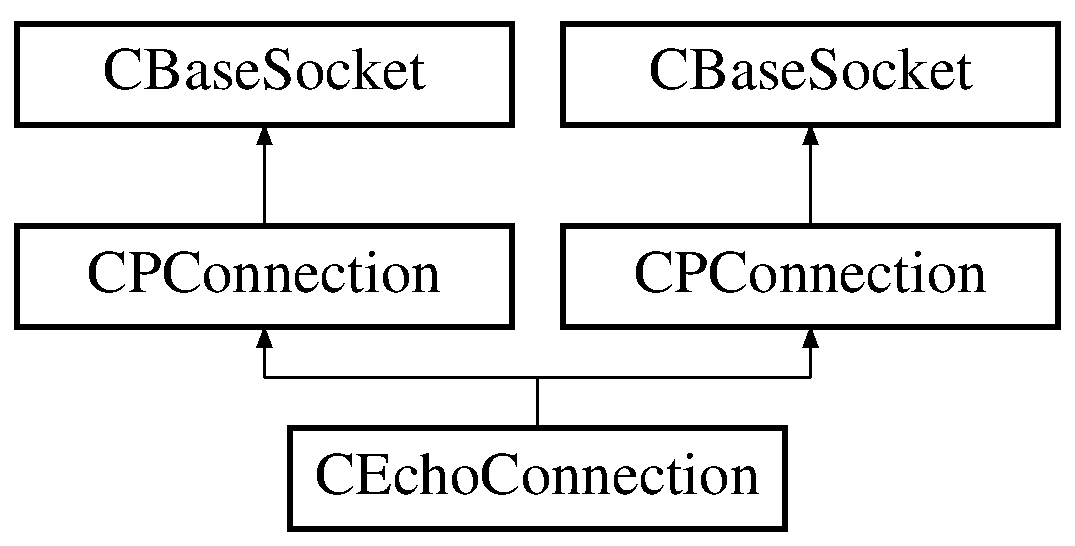
\includegraphics[height=3.000000cm]{class_c_echo_connection}
\end{center}
\end{figure}
\subsection*{\-Public \-Member \-Functions}
\begin{DoxyCompactItemize}
\item 
\hyperlink{class_c_echo_connection_a9ca0702071261601e37336232e08e531}{\-C\-Echo\-Connection} (\hyperlink{class_c_base_socket}{\-C\-Base\-Socket} $\ast$p\-Owner, struct sockaddr $\ast$p\-Addr=\-N\-U\-L\-L, int i\-Max\-Send\-Buffer\-Size=4096)
\item 
virtual \hyperlink{class_c_echo_connection_a61681b3f199d03d5e047b48f58310db1}{$\sim$\-C\-Echo\-Connection} ()
\item 
\hyperlink{_cpclient_8h_a3be13892ae7076009afcf121347dd319}{\-B\-O\-O\-L} \hyperlink{class_c_echo_connection_ac10d197eb5e2d1667dc044037f2151c5}{\-Process\-Data} (unsigned char $\ast$lp\-Data, int i\-Len)
\begin{DoxyCompactList}\small\item\em \-Pure virtual function to process data. \end{DoxyCompactList}\item 
\hyperlink{class_c_echo_connection_a9ca0702071261601e37336232e08e531}{\-C\-Echo\-Connection} (\hyperlink{class_c_base_socket}{\-C\-Base\-Socket} $\ast$p\-Owner, struct sockaddr $\ast$p\-Addr=\-N\-U\-L\-L, int i\-Max\-Send\-Buffer\-Size=4096)
\item 
virtual \hyperlink{class_c_echo_connection_a6a44ac933ebb5d0247fdc140306a2731}{$\sim$\-C\-Echo\-Connection} ()
\item 
\hyperlink{_cpclient_8h_a3be13892ae7076009afcf121347dd319}{\-B\-O\-O\-L} \hyperlink{class_c_echo_connection_ac10d197eb5e2d1667dc044037f2151c5}{\-Process\-Data} (unsigned char $\ast$lp\-Data, int i\-Len)
\begin{DoxyCompactList}\small\item\em \-Pure virtual function to process data. \end{DoxyCompactList}\end{DoxyCompactItemize}


\subsection{\-Detailed \-Description}


\-Definition at line 14 of file \-C\-Echo\-Connection.\-h.



\subsection{\-Constructor \& \-Destructor \-Documentation}
\hypertarget{class_c_echo_connection_a9ca0702071261601e37336232e08e531}{\index{\-C\-Echo\-Connection@{\-C\-Echo\-Connection}!\-C\-Echo\-Connection@{\-C\-Echo\-Connection}}
\index{\-C\-Echo\-Connection@{\-C\-Echo\-Connection}!CEchoConnection@{\-C\-Echo\-Connection}}
\subsubsection[{\-C\-Echo\-Connection}]{\setlength{\rightskip}{0pt plus 5cm}{\bf \-C\-Echo\-Connection\-::\-C\-Echo\-Connection} (
\begin{DoxyParamCaption}
\item[{{\bf \-C\-Base\-Socket} $\ast$}]{p\-Owner, }
\item[{struct sockaddr $\ast$}]{p\-Addr = {\ttfamily \-N\-U\-L\-L}, }
\item[{int}]{i\-Max\-Send\-Buffer\-Size = {\ttfamily 4096}}
\end{DoxyParamCaption}
)}}\label{class_c_echo_connection_a9ca0702071261601e37336232e08e531}


\-Definition at line 12 of file \-C\-Echo\-Connection.\-cpp.

\hypertarget{class_c_echo_connection_a61681b3f199d03d5e047b48f58310db1}{\index{\-C\-Echo\-Connection@{\-C\-Echo\-Connection}!$\sim$\-C\-Echo\-Connection@{$\sim$\-C\-Echo\-Connection}}
\index{$\sim$\-C\-Echo\-Connection@{$\sim$\-C\-Echo\-Connection}!CEchoConnection@{\-C\-Echo\-Connection}}
\subsubsection[{$\sim$\-C\-Echo\-Connection}]{\setlength{\rightskip}{0pt plus 5cm}{\bf \-C\-Echo\-Connection\-::$\sim$\-C\-Echo\-Connection} (
\begin{DoxyParamCaption}
{}
\end{DoxyParamCaption}
)\hspace{0.3cm}{\ttfamily  \mbox{[}virtual\mbox{]}}}}\label{class_c_echo_connection_a61681b3f199d03d5e047b48f58310db1}


\-Definition at line 19 of file \-C\-Echo\-Connection.\-cpp.

\hypertarget{class_c_echo_connection_a9ca0702071261601e37336232e08e531}{\index{\-C\-Echo\-Connection@{\-C\-Echo\-Connection}!\-C\-Echo\-Connection@{\-C\-Echo\-Connection}}
\index{\-C\-Echo\-Connection@{\-C\-Echo\-Connection}!CEchoConnection@{\-C\-Echo\-Connection}}
\subsubsection[{\-C\-Echo\-Connection}]{\setlength{\rightskip}{0pt plus 5cm}{\bf \-C\-Echo\-Connection\-::\-C\-Echo\-Connection} (
\begin{DoxyParamCaption}
\item[{{\bf \-C\-Base\-Socket} $\ast$}]{p\-Owner, }
\item[{struct sockaddr $\ast$}]{p\-Addr = {\ttfamily \-N\-U\-L\-L}, }
\item[{int}]{i\-Max\-Send\-Buffer\-Size = {\ttfamily 4096}}
\end{DoxyParamCaption}
)}}\label{class_c_echo_connection_a9ca0702071261601e37336232e08e531}
\hypertarget{class_c_echo_connection_a6a44ac933ebb5d0247fdc140306a2731}{\index{\-C\-Echo\-Connection@{\-C\-Echo\-Connection}!$\sim$\-C\-Echo\-Connection@{$\sim$\-C\-Echo\-Connection}}
\index{$\sim$\-C\-Echo\-Connection@{$\sim$\-C\-Echo\-Connection}!CEchoConnection@{\-C\-Echo\-Connection}}
\subsubsection[{$\sim$\-C\-Echo\-Connection}]{\setlength{\rightskip}{0pt plus 5cm}virtual {\bf \-C\-Echo\-Connection\-::$\sim$\-C\-Echo\-Connection} (
\begin{DoxyParamCaption}
{}
\end{DoxyParamCaption}
)\hspace{0.3cm}{\ttfamily  \mbox{[}virtual\mbox{]}}}}\label{class_c_echo_connection_a6a44ac933ebb5d0247fdc140306a2731}


\subsection{\-Member \-Function \-Documentation}
\hypertarget{class_c_echo_connection_ac10d197eb5e2d1667dc044037f2151c5}{\index{\-C\-Echo\-Connection@{\-C\-Echo\-Connection}!\-Process\-Data@{\-Process\-Data}}
\index{\-Process\-Data@{\-Process\-Data}!CEchoConnection@{\-C\-Echo\-Connection}}
\subsubsection[{\-Process\-Data}]{\setlength{\rightskip}{0pt plus 5cm}{\bf \-B\-O\-O\-L} {\bf \-C\-Echo\-Connection\-::\-Process\-Data} (
\begin{DoxyParamCaption}
\item[{unsigned char $\ast$}]{lp\-Data, }
\item[{int}]{i\-Len}
\end{DoxyParamCaption}
)\hspace{0.3cm}{\ttfamily  \mbox{[}virtual\mbox{]}}}}\label{class_c_echo_connection_ac10d197eb5e2d1667dc044037f2151c5}


\-Pure virtual function to process data. 



\-Implements \hyperlink{class_c_p_connection_a1b223eab8f518f390b2c01f7c1e33e72}{\-C\-P\-Connection}.



\-Definition at line 26 of file \-C\-Echo\-Connection.\-cpp.

\hypertarget{class_c_echo_connection_ac10d197eb5e2d1667dc044037f2151c5}{\index{\-C\-Echo\-Connection@{\-C\-Echo\-Connection}!\-Process\-Data@{\-Process\-Data}}
\index{\-Process\-Data@{\-Process\-Data}!CEchoConnection@{\-C\-Echo\-Connection}}
\subsubsection[{\-Process\-Data}]{\setlength{\rightskip}{0pt plus 5cm}{\bf \-B\-O\-O\-L} {\bf \-C\-Echo\-Connection\-::\-Process\-Data} (
\begin{DoxyParamCaption}
\item[{unsigned char $\ast$}]{lp\-Data, }
\item[{int}]{i\-Len}
\end{DoxyParamCaption}
)\hspace{0.3cm}{\ttfamily  \mbox{[}virtual\mbox{]}}}}\label{class_c_echo_connection_ac10d197eb5e2d1667dc044037f2151c5}


\-Pure virtual function to process data. 



\-Implements \hyperlink{class_c_p_connection_a1b223eab8f518f390b2c01f7c1e33e72}{\-C\-P\-Connection}.



\-The documentation for this class was generated from the following files\-:\begin{DoxyCompactItemize}
\item 
common/examples/\-C\-P\-\_\-examples/\-Test\-Client/\hyperlink{_test_client_2_c_echo_connection_8h}{\-C\-Echo\-Connection.\-h}\item 
common/examples/\-C\-P\-\_\-examples/\-Test\-Server/\hyperlink{_test_server_2_c_echo_connection_8h}{\-C\-Echo\-Connection.\-h}\item 
common/examples/\-C\-P\-\_\-examples/\-Test\-Client/\hyperlink{_test_client_2_c_echo_connection_8cpp}{\-C\-Echo\-Connection.\-cpp}\item 
common/examples/\-C\-P\-\_\-examples/\-Test\-Server/\hyperlink{_test_server_2_c_echo_connection_8cpp}{\-C\-Echo\-Connection.\-cpp}\end{DoxyCompactItemize}

\hypertarget{class_c_echo_server}{\section{\-C\-Echo\-Server \-Class \-Reference}
\label{class_c_echo_server}\index{\-C\-Echo\-Server@{\-C\-Echo\-Server}}
}


{\ttfamily \#include $<$\-C\-Echo\-Server.\-h$>$}

\-Inheritance diagram for \-C\-Echo\-Server\-:\begin{figure}[H]
\begin{center}
\leavevmode
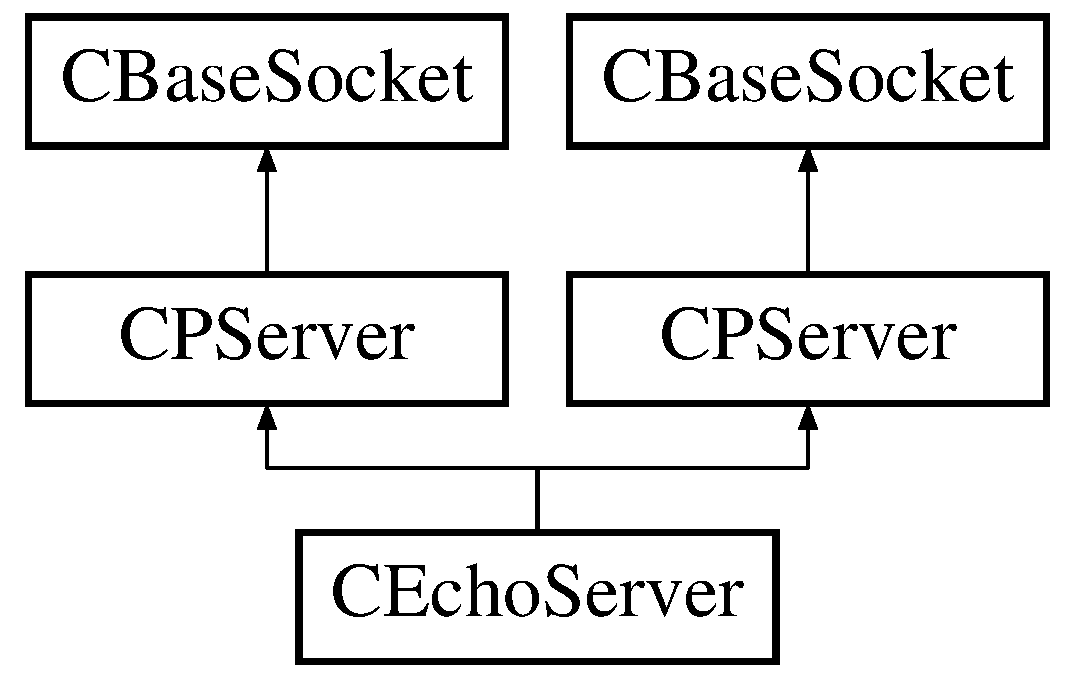
\includegraphics[height=3.000000cm]{class_c_echo_server}
\end{center}
\end{figure}
\subsection*{\-Public \-Member \-Functions}
\begin{DoxyCompactItemize}
\item 
\hyperlink{class_c_echo_server_a36cb9f59f793eef9a95b3d442d64ced4}{\-C\-Echo\-Server} (\-C\-P\-\_\-\-H\-A\-N\-D\-L\-E\-R\-\_\-\-A\-R\-R\-A\-Y \&c\-P\-Handlers)
\item 
virtual \hyperlink{class_c_echo_server_a2aab2a9ad38a750fb834392ba245f493}{$\sim$\-C\-Echo\-Server} ()
\item 
\hyperlink{class_c_p_connection}{\-C\-P\-Connection} $\ast$ \hyperlink{class_c_echo_server_a538eb049166aca7a0d27c7914c853876}{\-Allocate\-Socket\-Class} (struct sockaddr $\ast$p\-Addr)
\item 
\hyperlink{class_c_echo_server_a6bea4b7b0b87f08dc82e01537fc0000d}{\-C\-Echo\-Server} (\hyperlink{_c_p_connection_handler_8h_a05bf2fef946dbf14350a5f45bb28f953}{\-C\-P\-\_\-\-C\-O\-N\-N\-E\-C\-T\-I\-O\-N\-\_\-\-H\-A\-N\-D\-L\-E\-R\-\_\-\-A\-R\-R\-A\-Y} \&c\-P\-Handlers)
\item 
virtual \hyperlink{class_c_echo_server_a29b2422e3ec5976d2f4749db4e30cbad}{$\sim$\-C\-Echo\-Server} ()
\item 
\hyperlink{class_c_p_connection}{\-C\-P\-Connection} $\ast$ \hyperlink{class_c_echo_server_a8db4489876af267711eefbfd891bbb4d}{\-Allocate\-Socket\-Class} (struct sockaddr $\ast$p\-Addr)
\end{DoxyCompactItemize}


\subsection{\-Detailed \-Description}


\-Definition at line 14 of file \-C\-Echo\-Server.\-h.



\subsection{\-Constructor \& \-Destructor \-Documentation}
\hypertarget{class_c_echo_server_a36cb9f59f793eef9a95b3d442d64ced4}{\index{\-C\-Echo\-Server@{\-C\-Echo\-Server}!\-C\-Echo\-Server@{\-C\-Echo\-Server}}
\index{\-C\-Echo\-Server@{\-C\-Echo\-Server}!CEchoServer@{\-C\-Echo\-Server}}
\subsubsection[{\-C\-Echo\-Server}]{\setlength{\rightskip}{0pt plus 5cm}{\bf \-C\-Echo\-Server\-::\-C\-Echo\-Server} (
\begin{DoxyParamCaption}
\item[{\-C\-P\-\_\-\-H\-A\-N\-D\-L\-E\-R\-\_\-\-A\-R\-R\-A\-Y \&}]{c\-P\-Handlers}
\end{DoxyParamCaption}
)}}\label{class_c_echo_server_a36cb9f59f793eef9a95b3d442d64ced4}


\-Definition at line 13 of file \-C\-Echo\-Server.\-cpp.

\hypertarget{class_c_echo_server_a2aab2a9ad38a750fb834392ba245f493}{\index{\-C\-Echo\-Server@{\-C\-Echo\-Server}!$\sim$\-C\-Echo\-Server@{$\sim$\-C\-Echo\-Server}}
\index{$\sim$\-C\-Echo\-Server@{$\sim$\-C\-Echo\-Server}!CEchoServer@{\-C\-Echo\-Server}}
\subsubsection[{$\sim$\-C\-Echo\-Server}]{\setlength{\rightskip}{0pt plus 5cm}{\bf \-C\-Echo\-Server\-::$\sim$\-C\-Echo\-Server} (
\begin{DoxyParamCaption}
{}
\end{DoxyParamCaption}
)\hspace{0.3cm}{\ttfamily  \mbox{[}virtual\mbox{]}}}}\label{class_c_echo_server_a2aab2a9ad38a750fb834392ba245f493}


\-Definition at line 18 of file \-C\-Echo\-Server.\-cpp.

\hypertarget{class_c_echo_server_a6bea4b7b0b87f08dc82e01537fc0000d}{\index{\-C\-Echo\-Server@{\-C\-Echo\-Server}!\-C\-Echo\-Server@{\-C\-Echo\-Server}}
\index{\-C\-Echo\-Server@{\-C\-Echo\-Server}!CEchoServer@{\-C\-Echo\-Server}}
\subsubsection[{\-C\-Echo\-Server}]{\setlength{\rightskip}{0pt plus 5cm}{\bf \-C\-Echo\-Server\-::\-C\-Echo\-Server} (
\begin{DoxyParamCaption}
\item[{{\bf \-C\-P\-\_\-\-C\-O\-N\-N\-E\-C\-T\-I\-O\-N\-\_\-\-H\-A\-N\-D\-L\-E\-R\-\_\-\-A\-R\-R\-A\-Y} \&}]{c\-P\-Handlers}
\end{DoxyParamCaption}
)}}\label{class_c_echo_server_a6bea4b7b0b87f08dc82e01537fc0000d}


\-Definition at line 13 of file \-C\-Echo\-Server.\-cpp.

\hypertarget{class_c_echo_server_a29b2422e3ec5976d2f4749db4e30cbad}{\index{\-C\-Echo\-Server@{\-C\-Echo\-Server}!$\sim$\-C\-Echo\-Server@{$\sim$\-C\-Echo\-Server}}
\index{$\sim$\-C\-Echo\-Server@{$\sim$\-C\-Echo\-Server}!CEchoServer@{\-C\-Echo\-Server}}
\subsubsection[{$\sim$\-C\-Echo\-Server}]{\setlength{\rightskip}{0pt plus 5cm}virtual {\bf \-C\-Echo\-Server\-::$\sim$\-C\-Echo\-Server} (
\begin{DoxyParamCaption}
{}
\end{DoxyParamCaption}
)\hspace{0.3cm}{\ttfamily  \mbox{[}virtual\mbox{]}}}}\label{class_c_echo_server_a29b2422e3ec5976d2f4749db4e30cbad}


\subsection{\-Member \-Function \-Documentation}
\hypertarget{class_c_echo_server_a538eb049166aca7a0d27c7914c853876}{\index{\-C\-Echo\-Server@{\-C\-Echo\-Server}!\-Allocate\-Socket\-Class@{\-Allocate\-Socket\-Class}}
\index{\-Allocate\-Socket\-Class@{\-Allocate\-Socket\-Class}!CEchoServer@{\-C\-Echo\-Server}}
\subsubsection[{\-Allocate\-Socket\-Class}]{\setlength{\rightskip}{0pt plus 5cm}{\bf \-C\-P\-Connection} $\ast$ {\bf \-C\-Echo\-Server\-::\-Allocate\-Socket\-Class} (
\begin{DoxyParamCaption}
\item[{struct sockaddr $\ast$}]{p\-Addr}
\end{DoxyParamCaption}
)\hspace{0.3cm}{\ttfamily  \mbox{[}virtual\mbox{]}}}}\label{class_c_echo_server_a538eb049166aca7a0d27c7914c853876}
\-Pure virtual functions allocate and dallocate a derivative of \hyperlink{class_c_connection_socket}{\-C\-Connection\-Socket} \-Redefine in derived class 

\-Implements \hyperlink{class_c_p_server_ab028d102106a438f32c622596eaa1bc0}{\-C\-P\-Server}.



\-Definition at line 25 of file \-C\-Echo\-Server.\-cpp.

\hypertarget{class_c_echo_server_a8db4489876af267711eefbfd891bbb4d}{\index{\-C\-Echo\-Server@{\-C\-Echo\-Server}!\-Allocate\-Socket\-Class@{\-Allocate\-Socket\-Class}}
\index{\-Allocate\-Socket\-Class@{\-Allocate\-Socket\-Class}!CEchoServer@{\-C\-Echo\-Server}}
\subsubsection[{\-Allocate\-Socket\-Class}]{\setlength{\rightskip}{0pt plus 5cm}{\bf \-C\-P\-Connection}$\ast$ {\bf \-C\-Echo\-Server\-::\-Allocate\-Socket\-Class} (
\begin{DoxyParamCaption}
\item[{struct sockaddr $\ast$}]{p\-Addr}
\end{DoxyParamCaption}
)\hspace{0.3cm}{\ttfamily  \mbox{[}virtual\mbox{]}}}}\label{class_c_echo_server_a8db4489876af267711eefbfd891bbb4d}
\-Pure virtual functions allocate and dallocate a derivative of \hyperlink{class_c_connection_socket}{\-C\-Connection\-Socket} \-Redefine in derived class 

\-Implements \hyperlink{class_c_p_server_ab028d102106a438f32c622596eaa1bc0}{\-C\-P\-Server}.



\-The documentation for this class was generated from the following files\-:\begin{DoxyCompactItemize}
\item 
common/examples/\-C\-P\-\_\-examples/\-Test\-Client/\hyperlink{_test_client_2_c_echo_server_8h}{\-C\-Echo\-Server.\-h}\item 
common/examples/\-C\-P\-\_\-examples/\-Test\-Server/\hyperlink{_test_server_2_c_echo_server_8h}{\-C\-Echo\-Server.\-h}\item 
common/examples/\-C\-P\-\_\-examples/\-Test\-Client/\hyperlink{_test_client_2_c_echo_server_8cpp}{\-C\-Echo\-Server.\-cpp}\item 
common/examples/\-C\-P\-\_\-examples/\-Test\-Server/\hyperlink{_test_server_2_c_echo_server_8cpp}{\-C\-Echo\-Server.\-cpp}\end{DoxyCompactItemize}

\hypertarget{class_c_expat}{\section{\-C\-Expat \-Class \-Reference}
\label{class_c_expat}\index{\-C\-Expat@{\-C\-Expat}}
}


{\ttfamily \#include $<$\-Expat\-Impl.\-h$>$}

\-Inheritance diagram for \-C\-Expat\-:\begin{figure}[H]
\begin{center}
\leavevmode
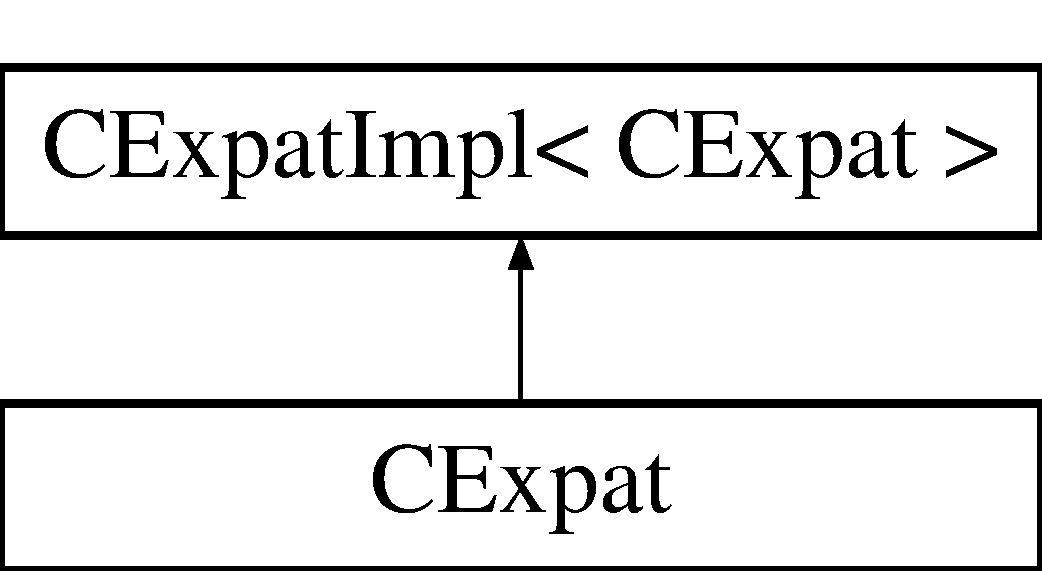
\includegraphics[height=2.000000cm]{class_c_expat}
\end{center}
\end{figure}
\subsection*{\-Public \-Member \-Functions}
\begin{DoxyCompactItemize}
\item 
\hyperlink{class_c_expat_a1aa7f71152f1863f2f0b6d8e1df64513}{\-C\-Expat} ()
\begin{DoxyCompactList}\small\item\em \-Constructors and destructors \end{DoxyCompactList}\item 
virtual \hyperlink{_cpclient_8h_a6464f7480a0fd0ee170cba12b2c0497f}{void} \hyperlink{class_c_expat_a60bd97eaa686c3a64d23dd07f3831db3}{\-On\-Start\-Element} (const \-X\-M\-L\-\_\-\-Char $\ast$psz\-Name, const \-X\-M\-L\-\_\-\-Char $\ast$$\ast$papsz\-Attrs)
\begin{DoxyCompactList}\small\item\em \-Public handler methods \end{DoxyCompactList}\item 
virtual \hyperlink{_cpclient_8h_a6464f7480a0fd0ee170cba12b2c0497f}{void} \hyperlink{class_c_expat_abff31a8eb9ea8ea0b0594ba8f497e8c4}{\-On\-End\-Element} (const \-X\-M\-L\-\_\-\-Char $\ast$psz\-Name)
\begin{DoxyCompactList}\small\item\em \-End element handler \end{DoxyCompactList}\item 
virtual \hyperlink{_cpclient_8h_a6464f7480a0fd0ee170cba12b2c0497f}{void} \hyperlink{class_c_expat_a4ee7b948e42f1c1a035fe386075d3691}{\-On\-Character\-Data} (const \-X\-M\-L\-\_\-\-Char $\ast$psz\-Data, int n\-Length)
\begin{DoxyCompactList}\small\item\em \-Character data handler \end{DoxyCompactList}\item 
virtual \hyperlink{_cpclient_8h_a6464f7480a0fd0ee170cba12b2c0497f}{void} \hyperlink{class_c_expat_a49a0c1058dd26ef680baea8af965778f}{\-On\-Processing\-Instruction} (const \-X\-M\-L\-\_\-\-Char $\ast$psz\-Target, const \-X\-M\-L\-\_\-\-Char $\ast$psz\-Data)
\begin{DoxyCompactList}\small\item\em \-Processing instruction handler \end{DoxyCompactList}\item 
virtual \hyperlink{_cpclient_8h_a6464f7480a0fd0ee170cba12b2c0497f}{void} \hyperlink{class_c_expat_a5c44bbfc76f1444880b40ddecae92007}{\-On\-Comment} (const \-X\-M\-L\-\_\-\-Char $\ast$psz\-Data)
\begin{DoxyCompactList}\small\item\em \-Comment handler \end{DoxyCompactList}\item 
virtual \hyperlink{_cpclient_8h_a6464f7480a0fd0ee170cba12b2c0497f}{void} \hyperlink{class_c_expat_a1ca4bcb887c156a9802d486de954d9c3}{\-On\-Start\-Cdata\-Section} ()
\begin{DoxyCompactList}\small\item\em \-Start \-C\-D\-A\-T\-A section handler \end{DoxyCompactList}\item 
virtual \hyperlink{_cpclient_8h_a6464f7480a0fd0ee170cba12b2c0497f}{void} \hyperlink{class_c_expat_ab35310a236f2035f8e1a0fda76ec7e31}{\-On\-End\-Cdata\-Section} ()
\begin{DoxyCompactList}\small\item\em \-End \-C\-D\-A\-T\-A section handler \end{DoxyCompactList}\item 
virtual \hyperlink{_cpclient_8h_a6464f7480a0fd0ee170cba12b2c0497f}{void} \hyperlink{class_c_expat_af2671ae016b05e929ba3937c4b68b575}{\-On\-Default} (const \-X\-M\-L\-\_\-\-Char $\ast$psz\-Data, int n\-Length)
\begin{DoxyCompactList}\small\item\em \-Default handler \end{DoxyCompactList}\item 
virtual bool \hyperlink{class_c_expat_a7ec0c8a7109b9dbe393c6cb09b9be420}{\-On\-External\-Entity\-Ref} (const \-X\-M\-L\-\_\-\-Char $\ast$psz\-Context, const \-X\-M\-L\-\_\-\-Char $\ast$psz\-Base, const \-X\-M\-L\-\_\-\-Char $\ast$psz\-System\-I\-D, const \-X\-M\-L\-\_\-\-Char $\ast$psz\-Public\-I\-D)
\begin{DoxyCompactList}\small\item\em \-External entity ref handler \end{DoxyCompactList}\item 
virtual bool \hyperlink{class_c_expat_a30d51f53c71a48084c46154676bed801}{\-On\-Unknown\-Encoding} (const \-X\-M\-L\-\_\-\-Char $\ast$psz\-Name, \-X\-M\-L\-\_\-\-Encoding $\ast$p\-Info)
\begin{DoxyCompactList}\small\item\em \-Unknown encoding handler \end{DoxyCompactList}\item 
virtual \hyperlink{_cpclient_8h_a6464f7480a0fd0ee170cba12b2c0497f}{void} \hyperlink{class_c_expat_ad0f1fb5aa04b76b6d6c52769d52cbf56}{\-On\-Start\-Namespace\-Decl} (const \-X\-M\-L\-\_\-\-Char $\ast$psz\-Prefix, const \-X\-M\-L\-\_\-\-Char $\ast$psz\-U\-R\-I)
\begin{DoxyCompactList}\small\item\em \-Start namespace declaration handler \end{DoxyCompactList}\item 
virtual \hyperlink{_cpclient_8h_a6464f7480a0fd0ee170cba12b2c0497f}{void} \hyperlink{class_c_expat_a8b2f35fc4bdc2c858cce7c2860b808f0}{\-On\-End\-Namespace\-Decl} (const \-X\-M\-L\-\_\-\-Char $\ast$psz\-Prefix)
\begin{DoxyCompactList}\small\item\em \-End namespace declaration handler \end{DoxyCompactList}\item 
virtual \hyperlink{_cpclient_8h_a6464f7480a0fd0ee170cba12b2c0497f}{void} \hyperlink{class_c_expat_a95a253c6c411ca157005faaa62ac2d8f}{\-On\-Xml\-Decl} (const \-X\-M\-L\-\_\-\-Char $\ast$psz\-Version, const \-X\-M\-L\-\_\-\-Char $\ast$psz\-Encoding, bool f\-Standalone)
\begin{DoxyCompactList}\small\item\em \-X\-M\-L declaration handler \end{DoxyCompactList}\item 
virtual \hyperlink{_cpclient_8h_a6464f7480a0fd0ee170cba12b2c0497f}{void} \hyperlink{class_c_expat_ad001e86058a374412bf6b61dedbca66b}{\-On\-Start\-Doctype\-Decl} (const \-X\-M\-L\-\_\-\-Char $\ast$psz\-Doctype\-Name, const \-X\-M\-L\-\_\-\-Char $\ast$psz\-Sys\-I\-D, const \-X\-M\-L\-\_\-\-Char $\ast$psz\-Pub\-I\-D, bool f\-Has\-Internal\-Subset)
\begin{DoxyCompactList}\small\item\em \-Start \-D\-O\-C\-T\-Y\-P\-E declaration handler \end{DoxyCompactList}\item 
virtual \hyperlink{_cpclient_8h_a6464f7480a0fd0ee170cba12b2c0497f}{void} \hyperlink{class_c_expat_abcb042b5d2b4ad02e3e1b28075315734}{\-On\-End\-Doctype\-Decl} ()
\begin{DoxyCompactList}\small\item\em \-End \-D\-O\-C\-T\-Y\-P\-E declaration handler \end{DoxyCompactList}\end{DoxyCompactItemize}


\subsection{\-Detailed \-Description}
-\/-\/-\/-\/-\/-\/-\/-\/-\/-\/-\/-\/-\/-\/-\/-\/-\/-\/-\/-\/-\/-\/-\/-\/-\/-\/-\/-\/-\/-\/-\/-\/-\/-\/-\/-\/-\/-\/-\/-\/-\/-\/-\/-\/-\/-\/-\/-\/-\/-\/-\/-\/-\/-\/-\/-\/-\/-\/-\/-\/-\/-\/-\/-\/-\/-\/-\/-\/-\/-\/-\/-\/-\/-\/-\/-\/-\/

\-Virtual method class definition

-\/-\/-\/-\/-\/-\/-\/-\/-\/-\/-\/-\/-\/-\/-\/-\/-\/-\/-\/-\/-\/-\/-\/-\/-\/-\/-\/-\/-\/-\/-\/-\/-\/-\/-\/-\/-\/-\/-\/-\/-\/-\/-\/-\/-\/-\/-\/-\/-\/-\/-\/-\/-\/-\/-\/-\/-\/-\/-\/-\/-\/-\/-\/-\/-\/-\/-\/-\/-\/-\/-\/-\/-\/-\/-\/-\/-\/ 

\-Definition at line 735 of file \-Expat\-Impl.\-h.



\subsection{\-Constructor \& \-Destructor \-Documentation}
\hypertarget{class_c_expat_a1aa7f71152f1863f2f0b6d8e1df64513}{\index{\-C\-Expat@{\-C\-Expat}!\-C\-Expat@{\-C\-Expat}}
\index{\-C\-Expat@{\-C\-Expat}!CExpat@{\-C\-Expat}}
\subsubsection[{\-C\-Expat}]{\setlength{\rightskip}{0pt plus 5cm}{\bf \-C\-Expat\-::\-C\-Expat} (
\begin{DoxyParamCaption}
{}
\end{DoxyParamCaption}
)\hspace{0.3cm}{\ttfamily  \mbox{[}inline\mbox{]}}}}\label{class_c_expat_a1aa7f71152f1863f2f0b6d8e1df64513}


\-Constructors and destructors 



\-Definition at line 740 of file \-Expat\-Impl.\-h.



\subsection{\-Member \-Function \-Documentation}
\hypertarget{class_c_expat_a4ee7b948e42f1c1a035fe386075d3691}{\index{\-C\-Expat@{\-C\-Expat}!\-On\-Character\-Data@{\-On\-Character\-Data}}
\index{\-On\-Character\-Data@{\-On\-Character\-Data}!CExpat@{\-C\-Expat}}
\subsubsection[{\-On\-Character\-Data}]{\setlength{\rightskip}{0pt plus 5cm}virtual {\bf void} {\bf \-C\-Expat\-::\-On\-Character\-Data} (
\begin{DoxyParamCaption}
\item[{const \-X\-M\-L\-\_\-\-Char $\ast$}]{psz\-Data, }
\item[{int}]{n\-Length}
\end{DoxyParamCaption}
)\hspace{0.3cm}{\ttfamily  \mbox{[}inline, virtual\mbox{]}}}}\label{class_c_expat_a4ee7b948e42f1c1a035fe386075d3691}


\-Character data handler 



\-Reimplemented from \hyperlink{class_c_expat_impl_ab97a7933f82395535706fa7a7584c2d4}{\-C\-Expat\-Impl$<$ C\-Expat $>$}.



\-Definition at line 764 of file \-Expat\-Impl.\-h.

\hypertarget{class_c_expat_a5c44bbfc76f1444880b40ddecae92007}{\index{\-C\-Expat@{\-C\-Expat}!\-On\-Comment@{\-On\-Comment}}
\index{\-On\-Comment@{\-On\-Comment}!CExpat@{\-C\-Expat}}
\subsubsection[{\-On\-Comment}]{\setlength{\rightskip}{0pt plus 5cm}virtual {\bf void} {\bf \-C\-Expat\-::\-On\-Comment} (
\begin{DoxyParamCaption}
\item[{const \-X\-M\-L\-\_\-\-Char $\ast$}]{psz\-Data}
\end{DoxyParamCaption}
)\hspace{0.3cm}{\ttfamily  \mbox{[}inline, virtual\mbox{]}}}}\label{class_c_expat_a5c44bbfc76f1444880b40ddecae92007}


\-Comment handler 



\-Reimplemented from \hyperlink{class_c_expat_impl_a3e107b5f2b8f3e0784e4bc3b21d9a954}{\-C\-Expat\-Impl$<$ C\-Expat $>$}.



\-Definition at line 779 of file \-Expat\-Impl.\-h.

\hypertarget{class_c_expat_af2671ae016b05e929ba3937c4b68b575}{\index{\-C\-Expat@{\-C\-Expat}!\-On\-Default@{\-On\-Default}}
\index{\-On\-Default@{\-On\-Default}!CExpat@{\-C\-Expat}}
\subsubsection[{\-On\-Default}]{\setlength{\rightskip}{0pt plus 5cm}virtual {\bf void} {\bf \-C\-Expat\-::\-On\-Default} (
\begin{DoxyParamCaption}
\item[{const \-X\-M\-L\-\_\-\-Char $\ast$}]{psz\-Data, }
\item[{int}]{n\-Length}
\end{DoxyParamCaption}
)\hspace{0.3cm}{\ttfamily  \mbox{[}inline, virtual\mbox{]}}}}\label{class_c_expat_af2671ae016b05e929ba3937c4b68b575}


\-Default handler 



\-Reimplemented from \hyperlink{class_c_expat_impl_a18a56a0963c1964ef785592a6c9cc7dc}{\-C\-Expat\-Impl$<$ C\-Expat $>$}.



\-Definition at line 800 of file \-Expat\-Impl.\-h.

\hypertarget{class_c_expat_ab35310a236f2035f8e1a0fda76ec7e31}{\index{\-C\-Expat@{\-C\-Expat}!\-On\-End\-Cdata\-Section@{\-On\-End\-Cdata\-Section}}
\index{\-On\-End\-Cdata\-Section@{\-On\-End\-Cdata\-Section}!CExpat@{\-C\-Expat}}
\subsubsection[{\-On\-End\-Cdata\-Section}]{\setlength{\rightskip}{0pt plus 5cm}virtual {\bf void} {\bf \-C\-Expat\-::\-On\-End\-Cdata\-Section} (
\begin{DoxyParamCaption}
{}
\end{DoxyParamCaption}
)\hspace{0.3cm}{\ttfamily  \mbox{[}inline, virtual\mbox{]}}}}\label{class_c_expat_ab35310a236f2035f8e1a0fda76ec7e31}


\-End \-C\-D\-A\-T\-A section handler 



\-Reimplemented from \hyperlink{class_c_expat_impl_af5fffe076811b52ef4de3e2399504c4c}{\-C\-Expat\-Impl$<$ C\-Expat $>$}.



\-Definition at line 793 of file \-Expat\-Impl.\-h.

\hypertarget{class_c_expat_abcb042b5d2b4ad02e3e1b28075315734}{\index{\-C\-Expat@{\-C\-Expat}!\-On\-End\-Doctype\-Decl@{\-On\-End\-Doctype\-Decl}}
\index{\-On\-End\-Doctype\-Decl@{\-On\-End\-Doctype\-Decl}!CExpat@{\-C\-Expat}}
\subsubsection[{\-On\-End\-Doctype\-Decl}]{\setlength{\rightskip}{0pt plus 5cm}virtual {\bf void} {\bf \-C\-Expat\-::\-On\-End\-Doctype\-Decl} (
\begin{DoxyParamCaption}
{}
\end{DoxyParamCaption}
)\hspace{0.3cm}{\ttfamily  \mbox{[}inline, virtual\mbox{]}}}}\label{class_c_expat_abcb042b5d2b4ad02e3e1b28075315734}


\-End \-D\-O\-C\-T\-Y\-P\-E declaration handler 



\-Reimplemented from \hyperlink{class_c_expat_impl_a395e6e654c41012cd3722d2445c174e3}{\-C\-Expat\-Impl$<$ C\-Expat $>$}.



\-Definition at line 855 of file \-Expat\-Impl.\-h.

\hypertarget{class_c_expat_abff31a8eb9ea8ea0b0594ba8f497e8c4}{\index{\-C\-Expat@{\-C\-Expat}!\-On\-End\-Element@{\-On\-End\-Element}}
\index{\-On\-End\-Element@{\-On\-End\-Element}!CExpat@{\-C\-Expat}}
\subsubsection[{\-On\-End\-Element}]{\setlength{\rightskip}{0pt plus 5cm}virtual {\bf void} {\bf \-C\-Expat\-::\-On\-End\-Element} (
\begin{DoxyParamCaption}
\item[{const \-X\-M\-L\-\_\-\-Char $\ast$}]{psz\-Name}
\end{DoxyParamCaption}
)\hspace{0.3cm}{\ttfamily  \mbox{[}inline, virtual\mbox{]}}}}\label{class_c_expat_abff31a8eb9ea8ea0b0594ba8f497e8c4}


\-End element handler 



\-Reimplemented from \hyperlink{class_c_expat_impl_aaf21a9a335c6daf7814e83006f968fa1}{\-C\-Expat\-Impl$<$ C\-Expat $>$}.



\-Definition at line 757 of file \-Expat\-Impl.\-h.

\hypertarget{class_c_expat_a8b2f35fc4bdc2c858cce7c2860b808f0}{\index{\-C\-Expat@{\-C\-Expat}!\-On\-End\-Namespace\-Decl@{\-On\-End\-Namespace\-Decl}}
\index{\-On\-End\-Namespace\-Decl@{\-On\-End\-Namespace\-Decl}!CExpat@{\-C\-Expat}}
\subsubsection[{\-On\-End\-Namespace\-Decl}]{\setlength{\rightskip}{0pt plus 5cm}virtual {\bf void} {\bf \-C\-Expat\-::\-On\-End\-Namespace\-Decl} (
\begin{DoxyParamCaption}
\item[{const \-X\-M\-L\-\_\-\-Char $\ast$}]{psz\-Prefix}
\end{DoxyParamCaption}
)\hspace{0.3cm}{\ttfamily  \mbox{[}inline, virtual\mbox{]}}}}\label{class_c_expat_a8b2f35fc4bdc2c858cce7c2860b808f0}


\-End namespace declaration handler 



\-Reimplemented from \hyperlink{class_c_expat_impl_a4aa22e82d10534373a7cf90354e4d9f2}{\-C\-Expat\-Impl$<$ C\-Expat $>$}.



\-Definition at line 831 of file \-Expat\-Impl.\-h.

\hypertarget{class_c_expat_a7ec0c8a7109b9dbe393c6cb09b9be420}{\index{\-C\-Expat@{\-C\-Expat}!\-On\-External\-Entity\-Ref@{\-On\-External\-Entity\-Ref}}
\index{\-On\-External\-Entity\-Ref@{\-On\-External\-Entity\-Ref}!CExpat@{\-C\-Expat}}
\subsubsection[{\-On\-External\-Entity\-Ref}]{\setlength{\rightskip}{0pt plus 5cm}virtual bool {\bf \-C\-Expat\-::\-On\-External\-Entity\-Ref} (
\begin{DoxyParamCaption}
\item[{const \-X\-M\-L\-\_\-\-Char $\ast$}]{psz\-Context, }
\item[{const \-X\-M\-L\-\_\-\-Char $\ast$}]{psz\-Base, }
\item[{const \-X\-M\-L\-\_\-\-Char $\ast$}]{psz\-System\-I\-D, }
\item[{const \-X\-M\-L\-\_\-\-Char $\ast$}]{psz\-Public\-I\-D}
\end{DoxyParamCaption}
)\hspace{0.3cm}{\ttfamily  \mbox{[}inline, virtual\mbox{]}}}}\label{class_c_expat_a7ec0c8a7109b9dbe393c6cb09b9be420}


\-External entity ref handler 



\-Reimplemented from \hyperlink{class_c_expat_impl_a413ff03445b1213314747265a1085d0a}{\-C\-Expat\-Impl$<$ C\-Expat $>$}.



\-Definition at line 807 of file \-Expat\-Impl.\-h.

\hypertarget{class_c_expat_a49a0c1058dd26ef680baea8af965778f}{\index{\-C\-Expat@{\-C\-Expat}!\-On\-Processing\-Instruction@{\-On\-Processing\-Instruction}}
\index{\-On\-Processing\-Instruction@{\-On\-Processing\-Instruction}!CExpat@{\-C\-Expat}}
\subsubsection[{\-On\-Processing\-Instruction}]{\setlength{\rightskip}{0pt plus 5cm}virtual {\bf void} {\bf \-C\-Expat\-::\-On\-Processing\-Instruction} (
\begin{DoxyParamCaption}
\item[{const \-X\-M\-L\-\_\-\-Char $\ast$}]{psz\-Target, }
\item[{const \-X\-M\-L\-\_\-\-Char $\ast$}]{psz\-Data}
\end{DoxyParamCaption}
)\hspace{0.3cm}{\ttfamily  \mbox{[}inline, virtual\mbox{]}}}}\label{class_c_expat_a49a0c1058dd26ef680baea8af965778f}


\-Processing instruction handler 



\-Reimplemented from \hyperlink{class_c_expat_impl_a403235345e254d13e69124b47c0160d8}{\-C\-Expat\-Impl$<$ C\-Expat $>$}.



\-Definition at line 771 of file \-Expat\-Impl.\-h.

\hypertarget{class_c_expat_a1ca4bcb887c156a9802d486de954d9c3}{\index{\-C\-Expat@{\-C\-Expat}!\-On\-Start\-Cdata\-Section@{\-On\-Start\-Cdata\-Section}}
\index{\-On\-Start\-Cdata\-Section@{\-On\-Start\-Cdata\-Section}!CExpat@{\-C\-Expat}}
\subsubsection[{\-On\-Start\-Cdata\-Section}]{\setlength{\rightskip}{0pt plus 5cm}virtual {\bf void} {\bf \-C\-Expat\-::\-On\-Start\-Cdata\-Section} (
\begin{DoxyParamCaption}
{}
\end{DoxyParamCaption}
)\hspace{0.3cm}{\ttfamily  \mbox{[}inline, virtual\mbox{]}}}}\label{class_c_expat_a1ca4bcb887c156a9802d486de954d9c3}


\-Start \-C\-D\-A\-T\-A section handler 



\-Reimplemented from \hyperlink{class_c_expat_impl_a5a7082a8c80f14cfed55edc084e1a448}{\-C\-Expat\-Impl$<$ C\-Expat $>$}.



\-Definition at line 786 of file \-Expat\-Impl.\-h.

\hypertarget{class_c_expat_ad001e86058a374412bf6b61dedbca66b}{\index{\-C\-Expat@{\-C\-Expat}!\-On\-Start\-Doctype\-Decl@{\-On\-Start\-Doctype\-Decl}}
\index{\-On\-Start\-Doctype\-Decl@{\-On\-Start\-Doctype\-Decl}!CExpat@{\-C\-Expat}}
\subsubsection[{\-On\-Start\-Doctype\-Decl}]{\setlength{\rightskip}{0pt plus 5cm}virtual {\bf void} {\bf \-C\-Expat\-::\-On\-Start\-Doctype\-Decl} (
\begin{DoxyParamCaption}
\item[{const \-X\-M\-L\-\_\-\-Char $\ast$}]{psz\-Doctype\-Name, }
\item[{const \-X\-M\-L\-\_\-\-Char $\ast$}]{psz\-Sys\-I\-D, }
\item[{const \-X\-M\-L\-\_\-\-Char $\ast$}]{psz\-Pub\-I\-D, }
\item[{bool}]{f\-Has\-Internal\-Subset}
\end{DoxyParamCaption}
)\hspace{0.3cm}{\ttfamily  \mbox{[}inline, virtual\mbox{]}}}}\label{class_c_expat_ad001e86058a374412bf6b61dedbca66b}


\-Start \-D\-O\-C\-T\-Y\-P\-E declaration handler 



\-Reimplemented from \hyperlink{class_c_expat_impl_a98aee5e2d5b4e00b4808e3b6b6761872}{\-C\-Expat\-Impl$<$ C\-Expat $>$}.



\-Definition at line 846 of file \-Expat\-Impl.\-h.

\hypertarget{class_c_expat_a60bd97eaa686c3a64d23dd07f3831db3}{\index{\-C\-Expat@{\-C\-Expat}!\-On\-Start\-Element@{\-On\-Start\-Element}}
\index{\-On\-Start\-Element@{\-On\-Start\-Element}!CExpat@{\-C\-Expat}}
\subsubsection[{\-On\-Start\-Element}]{\setlength{\rightskip}{0pt plus 5cm}virtual {\bf void} {\bf \-C\-Expat\-::\-On\-Start\-Element} (
\begin{DoxyParamCaption}
\item[{const \-X\-M\-L\-\_\-\-Char $\ast$}]{psz\-Name, }
\item[{const \-X\-M\-L\-\_\-\-Char $\ast$$\ast$}]{papsz\-Attrs}
\end{DoxyParamCaption}
)\hspace{0.3cm}{\ttfamily  \mbox{[}inline, virtual\mbox{]}}}}\label{class_c_expat_a60bd97eaa686c3a64d23dd07f3831db3}


\-Public handler methods 

\-Start element handler 

\-Reimplemented from \hyperlink{class_c_expat_impl_a94c5469966d0124253e2b67eda7d59ff}{\-C\-Expat\-Impl$<$ C\-Expat $>$}.



\-Definition at line 749 of file \-Expat\-Impl.\-h.

\hypertarget{class_c_expat_ad0f1fb5aa04b76b6d6c52769d52cbf56}{\index{\-C\-Expat@{\-C\-Expat}!\-On\-Start\-Namespace\-Decl@{\-On\-Start\-Namespace\-Decl}}
\index{\-On\-Start\-Namespace\-Decl@{\-On\-Start\-Namespace\-Decl}!CExpat@{\-C\-Expat}}
\subsubsection[{\-On\-Start\-Namespace\-Decl}]{\setlength{\rightskip}{0pt plus 5cm}virtual {\bf void} {\bf \-C\-Expat\-::\-On\-Start\-Namespace\-Decl} (
\begin{DoxyParamCaption}
\item[{const \-X\-M\-L\-\_\-\-Char $\ast$}]{psz\-Prefix, }
\item[{const \-X\-M\-L\-\_\-\-Char $\ast$}]{psz\-U\-R\-I}
\end{DoxyParamCaption}
)\hspace{0.3cm}{\ttfamily  \mbox{[}inline, virtual\mbox{]}}}}\label{class_c_expat_ad0f1fb5aa04b76b6d6c52769d52cbf56}


\-Start namespace declaration handler 



\-Reimplemented from \hyperlink{class_c_expat_impl_a6e40ab1481ae7a0b498d390050467886}{\-C\-Expat\-Impl$<$ C\-Expat $>$}.



\-Definition at line 823 of file \-Expat\-Impl.\-h.

\hypertarget{class_c_expat_a30d51f53c71a48084c46154676bed801}{\index{\-C\-Expat@{\-C\-Expat}!\-On\-Unknown\-Encoding@{\-On\-Unknown\-Encoding}}
\index{\-On\-Unknown\-Encoding@{\-On\-Unknown\-Encoding}!CExpat@{\-C\-Expat}}
\subsubsection[{\-On\-Unknown\-Encoding}]{\setlength{\rightskip}{0pt plus 5cm}virtual bool {\bf \-C\-Expat\-::\-On\-Unknown\-Encoding} (
\begin{DoxyParamCaption}
\item[{const \-X\-M\-L\-\_\-\-Char $\ast$}]{psz\-Name, }
\item[{\-X\-M\-L\-\_\-\-Encoding $\ast$}]{p\-Info}
\end{DoxyParamCaption}
)\hspace{0.3cm}{\ttfamily  \mbox{[}inline, virtual\mbox{]}}}}\label{class_c_expat_a30d51f53c71a48084c46154676bed801}


\-Unknown encoding handler 



\-Reimplemented from \hyperlink{class_c_expat_impl_a17863cd62866c6895319a99c46ec56e1}{\-C\-Expat\-Impl$<$ C\-Expat $>$}.



\-Definition at line 816 of file \-Expat\-Impl.\-h.

\hypertarget{class_c_expat_a95a253c6c411ca157005faaa62ac2d8f}{\index{\-C\-Expat@{\-C\-Expat}!\-On\-Xml\-Decl@{\-On\-Xml\-Decl}}
\index{\-On\-Xml\-Decl@{\-On\-Xml\-Decl}!CExpat@{\-C\-Expat}}
\subsubsection[{\-On\-Xml\-Decl}]{\setlength{\rightskip}{0pt plus 5cm}virtual {\bf void} {\bf \-C\-Expat\-::\-On\-Xml\-Decl} (
\begin{DoxyParamCaption}
\item[{const \-X\-M\-L\-\_\-\-Char $\ast$}]{psz\-Version, }
\item[{const \-X\-M\-L\-\_\-\-Char $\ast$}]{psz\-Encoding, }
\item[{bool}]{f\-Standalone}
\end{DoxyParamCaption}
)\hspace{0.3cm}{\ttfamily  \mbox{[}inline, virtual\mbox{]}}}}\label{class_c_expat_a95a253c6c411ca157005faaa62ac2d8f}


\-X\-M\-L declaration handler 



\-Reimplemented from \hyperlink{class_c_expat_impl_a852c68ceb2b2527ff04a245eeac51dfa}{\-C\-Expat\-Impl$<$ C\-Expat $>$}.



\-Definition at line 838 of file \-Expat\-Impl.\-h.



\-The documentation for this class was generated from the following file\-:\begin{DoxyCompactItemize}
\item 
common/expat/\hyperlink{_expat_impl_8h}{\-Expat\-Impl.\-h}\end{DoxyCompactItemize}

\hypertarget{class_c_expat_impl}{\section{\-C\-Expat\-Impl$<$ \-\_\-\-T $>$ \-Class \-Template \-Reference}
\label{class_c_expat_impl}\index{\-C\-Expat\-Impl$<$ \-\_\-\-T $>$@{\-C\-Expat\-Impl$<$ \-\_\-\-T $>$}}
}


{\ttfamily \#include $<$\-Expat\-Impl.\-h$>$}

\subsection*{\-Public \-Member \-Functions}
\begin{DoxyCompactItemize}
\item 
\hyperlink{class_c_expat_impl_a59f688f607c739742ef3ac272ea02fee}{\-C\-Expat\-Impl} ()
\begin{DoxyCompactList}\small\item\em \-Constructors and destructors \end{DoxyCompactList}\item 
\hyperlink{class_c_expat_impl_a6905e278a30c7f7331001ab89f249c63}{$\sim$\-C\-Expat\-Impl} ()
\begin{DoxyCompactList}\small\item\em \-Destructor \end{DoxyCompactList}\item 
bool \hyperlink{class_c_expat_impl_ada29fce37e448ceb6ea09a98de028149}{\-Create} (const \-X\-M\-L\-\_\-\-Char $\ast$psz\-Encoding=\-N\-U\-L\-L, const \-X\-M\-L\-\_\-\-Char $\ast$psz\-Sep=\-N\-U\-L\-L)
\begin{DoxyCompactList}\small\item\em \-Parser creation and deletion methods \end{DoxyCompactList}\item 
\hyperlink{_cpclient_8h_a6464f7480a0fd0ee170cba12b2c0497f}{void} \hyperlink{class_c_expat_impl_a2e4dcba61823bcc922b1348fcbe787db}{\-Destroy} ()
\begin{DoxyCompactList}\small\item\em \-Destroy the parser \end{DoxyCompactList}\item 
bool \hyperlink{class_c_expat_impl_a76062f116c2a9c99d42631da6e806339}{\-Parse} (const char $\ast$psz\-Buffer, int n\-Length=-\/1, bool f\-Is\-Final=true)
\begin{DoxyCompactList}\small\item\em \-Parser parse methods \end{DoxyCompactList}\item 
bool \hyperlink{class_c_expat_impl_a35df06396bfa8330598572a3f530a5c1}{\-Parse\-Buffer} (int n\-Length, bool f\-Is\-Final=true)
\begin{DoxyCompactList}\small\item\em \-Parse a block of data \end{DoxyCompactList}\item 
\hyperlink{_cpclient_8h_a6464f7480a0fd0ee170cba12b2c0497f}{void} $\ast$ \hyperlink{class_c_expat_impl_ae9b6bb575b4a81c24384a13433113925}{\-Get\-Buffer} (int n\-Length)
\begin{DoxyCompactList}\small\item\em \-Get the internal buffer \end{DoxyCompactList}\item 
\hyperlink{_cpclient_8h_a6464f7480a0fd0ee170cba12b2c0497f}{void} \hyperlink{class_c_expat_impl_a17a24b6c1c157f3c843e730f3f796667}{\-Enable\-Start\-Element\-Handler} (bool f\-Enable=true)
\begin{DoxyCompactList}\small\item\em \-Parser callback enable/disable methods \end{DoxyCompactList}\item 
\hyperlink{_cpclient_8h_a6464f7480a0fd0ee170cba12b2c0497f}{void} \hyperlink{class_c_expat_impl_ac91830d2f654065a22d7331af20a3568}{\-Enable\-End\-Element\-Handler} (bool f\-Enable=true)
\begin{DoxyCompactList}\small\item\em \-Enable/\-Disable the end element handler \end{DoxyCompactList}\item 
\hyperlink{_cpclient_8h_a6464f7480a0fd0ee170cba12b2c0497f}{void} \hyperlink{class_c_expat_impl_acf2e51e7fb9183a180cd8ffdc8bebb3e}{\-Enable\-Element\-Handler} (bool f\-Enable=true)
\begin{DoxyCompactList}\small\item\em \-Enable/\-Disable the element handlers \end{DoxyCompactList}\item 
\hyperlink{_cpclient_8h_a6464f7480a0fd0ee170cba12b2c0497f}{void} \hyperlink{class_c_expat_impl_a9710ebe6b824dd35fc3cffe748df9749}{\-Enable\-Character\-Data\-Handler} (bool f\-Enable=true)
\begin{DoxyCompactList}\small\item\em \-Enable/\-Disable the character data handler \end{DoxyCompactList}\item 
\hyperlink{_cpclient_8h_a6464f7480a0fd0ee170cba12b2c0497f}{void} \hyperlink{class_c_expat_impl_ad645eca4eb59c0faa6425a20f6a05595}{\-Enable\-Processing\-Instruction\-Handler} (bool f\-Enable=true)
\begin{DoxyCompactList}\small\item\em \-Enable/\-Disable the processing instruction handler \end{DoxyCompactList}\item 
\hyperlink{_cpclient_8h_a6464f7480a0fd0ee170cba12b2c0497f}{void} \hyperlink{class_c_expat_impl_a552c6281c12de7a74e17df3faf38723b}{\-Enable\-Comment\-Handler} (bool f\-Enable=true)
\begin{DoxyCompactList}\small\item\em \-Enable/\-Disable the comment handler \end{DoxyCompactList}\item 
\hyperlink{_cpclient_8h_a6464f7480a0fd0ee170cba12b2c0497f}{void} \hyperlink{class_c_expat_impl_a27ad6538ae5e773fc2d6af0ff8441582}{\-Enable\-Start\-Cdata\-Section\-Handler} (bool f\-Enable=true)
\begin{DoxyCompactList}\small\item\em \-Enable/\-Disable the start \-C\-D\-A\-T\-A section handler \end{DoxyCompactList}\item 
\hyperlink{_cpclient_8h_a6464f7480a0fd0ee170cba12b2c0497f}{void} \hyperlink{class_c_expat_impl_a3390e7ef5fc411b0d76da2cc3528231d}{\-Enable\-End\-Cdata\-Section\-Handler} (bool f\-Enable=true)
\begin{DoxyCompactList}\small\item\em \-Enable/\-Disable the end \-C\-D\-A\-T\-A section handler \end{DoxyCompactList}\item 
\hyperlink{_cpclient_8h_a6464f7480a0fd0ee170cba12b2c0497f}{void} \hyperlink{class_c_expat_impl_ad0b0fa3d2c7604d0af6f8b4662d17c38}{\-Enable\-Cdata\-Section\-Handler} (bool f\-Enable=true)
\begin{DoxyCompactList}\small\item\em \-Enable/\-Disable the \-C\-D\-A\-T\-A section handlers \end{DoxyCompactList}\item 
\hyperlink{_cpclient_8h_a6464f7480a0fd0ee170cba12b2c0497f}{void} \hyperlink{class_c_expat_impl_a79ccb0e194a01a82e67f0d75a05ff4dc}{\-Enable\-Default\-Handler} (bool f\-Enable=true, bool f\-Expand=true)
\begin{DoxyCompactList}\small\item\em \-Enable/\-Disable default handler \end{DoxyCompactList}\item 
\hyperlink{_cpclient_8h_a6464f7480a0fd0ee170cba12b2c0497f}{void} \hyperlink{class_c_expat_impl_a792a4fedfcde46489c261e692eea54f4}{\-Enable\-External\-Entity\-Ref\-Handler} (bool f\-Enable=true)
\begin{DoxyCompactList}\small\item\em \-Enable/\-Disable external entity ref handler \end{DoxyCompactList}\item 
\hyperlink{_cpclient_8h_a6464f7480a0fd0ee170cba12b2c0497f}{void} \hyperlink{class_c_expat_impl_a784e4d39f69b56f02d3e2a85eaeb641b}{\-Enable\-Unknown\-Encoding\-Handler} (bool f\-Enable=true)
\begin{DoxyCompactList}\small\item\em \-Enable/\-Disable unknown encoding handler \end{DoxyCompactList}\item 
\hyperlink{_cpclient_8h_a6464f7480a0fd0ee170cba12b2c0497f}{void} \hyperlink{class_c_expat_impl_ac675f52624f52b3cdaa57b86d97d7f51}{\-Enable\-Start\-Namespace\-Decl\-Handler} (bool f\-Enable=true)
\begin{DoxyCompactList}\small\item\em \-Enable/\-Disable start namespace handler \end{DoxyCompactList}\item 
\hyperlink{_cpclient_8h_a6464f7480a0fd0ee170cba12b2c0497f}{void} \hyperlink{class_c_expat_impl_ae3938fc6542d2f56c88934dd4d7c70ee}{\-Enable\-End\-Namespace\-Decl\-Handler} (bool f\-Enable=true)
\begin{DoxyCompactList}\small\item\em \-Enable/\-Disable end namespace handler \end{DoxyCompactList}\item 
\hyperlink{_cpclient_8h_a6464f7480a0fd0ee170cba12b2c0497f}{void} \hyperlink{class_c_expat_impl_a7b3c35dc2f667aa146f346a2b437bd54}{\-Enable\-Namespace\-Decl\-Handler} (bool f\-Enable=true)
\begin{DoxyCompactList}\small\item\em \-Enable/\-Disable namespace handlers \end{DoxyCompactList}\item 
\hyperlink{_cpclient_8h_a6464f7480a0fd0ee170cba12b2c0497f}{void} \hyperlink{class_c_expat_impl_afffef6ef64c80c88786cf06b4ba9e776}{\-Enable\-Xml\-Decl\-Handler} (bool f\-Enable=true)
\begin{DoxyCompactList}\small\item\em \-Enable/\-Disable the \-X\-M\-L declaration handler \end{DoxyCompactList}\item 
\hyperlink{_cpclient_8h_a6464f7480a0fd0ee170cba12b2c0497f}{void} \hyperlink{class_c_expat_impl_a1294cb39e231da87e282eb84196c8785}{\-Enable\-Start\-Doctype\-Decl\-Handler} (bool f\-Enable=true)
\begin{DoxyCompactList}\small\item\em \-Enable/\-Disable the start \-D\-O\-C\-T\-Y\-P\-E declaration handler \end{DoxyCompactList}\item 
\hyperlink{_cpclient_8h_a6464f7480a0fd0ee170cba12b2c0497f}{void} \hyperlink{class_c_expat_impl_a6fcf5de29a3e7a3da9ca655eb91b115c}{\-Enable\-End\-Doctype\-Decl\-Handler} (bool f\-Enable=true)
\begin{DoxyCompactList}\small\item\em \-Enable/\-Disable the end \-D\-O\-C\-T\-Y\-P\-E declaration handler \end{DoxyCompactList}\item 
\hyperlink{_cpclient_8h_a6464f7480a0fd0ee170cba12b2c0497f}{void} \hyperlink{class_c_expat_impl_a267c2e407879948b0b3910ccc84e7815}{\-Enable\-Doctype\-Decl\-Handler} (bool f\-Enable=true)
\begin{DoxyCompactList}\small\item\em \-Enable/\-Disable the \-D\-O\-C\-T\-Y\-P\-E declaration handler \end{DoxyCompactList}\item 
enum \-X\-M\-L\-\_\-\-Error \hyperlink{class_c_expat_impl_aeb0f6e67c9ab6fdfeb299f48d8445837}{\-Get\-Error\-Code} ()
\begin{DoxyCompactList}\small\item\em \-Parser error reporting methods \end{DoxyCompactList}\item 
long \hyperlink{class_c_expat_impl_ab19268d1441402b98ec8ccab31cb2015}{\-Get\-Current\-Byte\-Index} ()
\begin{DoxyCompactList}\small\item\em \-Get the current byte index \end{DoxyCompactList}\item 
int \hyperlink{class_c_expat_impl_ab6ef6ce8ef73ed2a454f6375ab7b665f}{\-Get\-Current\-Line\-Number} ()
\begin{DoxyCompactList}\small\item\em \-Get the current line number \end{DoxyCompactList}\item 
int \hyperlink{class_c_expat_impl_aad097c9be6cd886a799eee992670d9de}{\-Get\-Current\-Column\-Number} ()
\begin{DoxyCompactList}\small\item\em \-Get the current column number \end{DoxyCompactList}\item 
int \hyperlink{class_c_expat_impl_a984d18a346ce61788df2f697e1f3ab61}{\-Get\-Current\-Byte\-Count} ()
\begin{DoxyCompactList}\small\item\em \-Get the current byte count \end{DoxyCompactList}\item 
const char $\ast$ \hyperlink{class_c_expat_impl_a9d270067e041578c57eb71a1238ed717}{\-Get\-Input\-Context} (int $\ast$pn\-Offset, int $\ast$pn\-Size)
\begin{DoxyCompactList}\small\item\em \-Get the input context \end{DoxyCompactList}\item 
const \-X\-M\-L\-\_\-\-L\-Char $\ast$ \hyperlink{class_c_expat_impl_af463b2fa4776e97d9c0f62fc8333f9f6}{\-Get\-Error\-String} ()
\begin{DoxyCompactList}\small\item\em \-Get last error string \end{DoxyCompactList}\item 
\hyperlink{_cpclient_8h_a6464f7480a0fd0ee170cba12b2c0497f}{void} \hyperlink{class_c_expat_impl_a94c5469966d0124253e2b67eda7d59ff}{\-On\-Start\-Element} (const \-X\-M\-L\-\_\-\-Char $\ast$psz\-Name, const \-X\-M\-L\-\_\-\-Char $\ast$$\ast$papsz\-Attrs)
\begin{DoxyCompactList}\small\item\em \-Public handler methods \end{DoxyCompactList}\item 
\hyperlink{_cpclient_8h_a6464f7480a0fd0ee170cba12b2c0497f}{void} \hyperlink{class_c_expat_impl_aaf21a9a335c6daf7814e83006f968fa1}{\-On\-End\-Element} (const \-X\-M\-L\-\_\-\-Char $\ast$psz\-Name)
\begin{DoxyCompactList}\small\item\em \-End element handler \end{DoxyCompactList}\item 
\hyperlink{_cpclient_8h_a6464f7480a0fd0ee170cba12b2c0497f}{void} \hyperlink{class_c_expat_impl_ab97a7933f82395535706fa7a7584c2d4}{\-On\-Character\-Data} (const \-X\-M\-L\-\_\-\-Char $\ast$psz\-Data, int n\-Length)
\begin{DoxyCompactList}\small\item\em \-Character data handler \end{DoxyCompactList}\item 
\hyperlink{_cpclient_8h_a6464f7480a0fd0ee170cba12b2c0497f}{void} \hyperlink{class_c_expat_impl_a403235345e254d13e69124b47c0160d8}{\-On\-Processing\-Instruction} (const \-X\-M\-L\-\_\-\-Char $\ast$psz\-Target, const \-X\-M\-L\-\_\-\-Char $\ast$psz\-Data)
\begin{DoxyCompactList}\small\item\em \-Processing instruction handler \end{DoxyCompactList}\item 
\hyperlink{_cpclient_8h_a6464f7480a0fd0ee170cba12b2c0497f}{void} \hyperlink{class_c_expat_impl_a3e107b5f2b8f3e0784e4bc3b21d9a954}{\-On\-Comment} (const \-X\-M\-L\-\_\-\-Char $\ast$psz\-Data)
\begin{DoxyCompactList}\small\item\em \-Comment handler \end{DoxyCompactList}\item 
\hyperlink{_cpclient_8h_a6464f7480a0fd0ee170cba12b2c0497f}{void} \hyperlink{class_c_expat_impl_a5a7082a8c80f14cfed55edc084e1a448}{\-On\-Start\-Cdata\-Section} ()
\begin{DoxyCompactList}\small\item\em \-Start \-C\-D\-A\-T\-A section handler \end{DoxyCompactList}\item 
\hyperlink{_cpclient_8h_a6464f7480a0fd0ee170cba12b2c0497f}{void} \hyperlink{class_c_expat_impl_af5fffe076811b52ef4de3e2399504c4c}{\-On\-End\-Cdata\-Section} ()
\begin{DoxyCompactList}\small\item\em \-End \-C\-D\-A\-T\-A section handler \end{DoxyCompactList}\item 
\hyperlink{_cpclient_8h_a6464f7480a0fd0ee170cba12b2c0497f}{void} \hyperlink{class_c_expat_impl_a18a56a0963c1964ef785592a6c9cc7dc}{\-On\-Default} (const \-X\-M\-L\-\_\-\-Char $\ast$psz\-Data, int n\-Length)
\begin{DoxyCompactList}\small\item\em \-Default handler \end{DoxyCompactList}\item 
bool \hyperlink{class_c_expat_impl_a413ff03445b1213314747265a1085d0a}{\-On\-External\-Entity\-Ref} (const \-X\-M\-L\-\_\-\-Char $\ast$psz\-Context, const \-X\-M\-L\-\_\-\-Char $\ast$psz\-Base, const \-X\-M\-L\-\_\-\-Char $\ast$psz\-System\-I\-D, const \-X\-M\-L\-\_\-\-Char $\ast$psz\-Public\-I\-D)
\begin{DoxyCompactList}\small\item\em \-External entity ref handler \end{DoxyCompactList}\item 
bool \hyperlink{class_c_expat_impl_a17863cd62866c6895319a99c46ec56e1}{\-On\-Unknown\-Encoding} (const \-X\-M\-L\-\_\-\-Char $\ast$psz\-Name, \-X\-M\-L\-\_\-\-Encoding $\ast$p\-Info)
\begin{DoxyCompactList}\small\item\em \-Unknown encoding handler \end{DoxyCompactList}\item 
\hyperlink{_cpclient_8h_a6464f7480a0fd0ee170cba12b2c0497f}{void} \hyperlink{class_c_expat_impl_a6e40ab1481ae7a0b498d390050467886}{\-On\-Start\-Namespace\-Decl} (const \-X\-M\-L\-\_\-\-Char $\ast$psz\-Prefix, const \-X\-M\-L\-\_\-\-Char $\ast$psz\-U\-R\-I)
\begin{DoxyCompactList}\small\item\em \-Start namespace declaration handler \end{DoxyCompactList}\item 
\hyperlink{_cpclient_8h_a6464f7480a0fd0ee170cba12b2c0497f}{void} \hyperlink{class_c_expat_impl_a4aa22e82d10534373a7cf90354e4d9f2}{\-On\-End\-Namespace\-Decl} (const \-X\-M\-L\-\_\-\-Char $\ast$psz\-Prefix)
\begin{DoxyCompactList}\small\item\em \-End namespace declaration handler \end{DoxyCompactList}\item 
\hyperlink{_cpclient_8h_a6464f7480a0fd0ee170cba12b2c0497f}{void} \hyperlink{class_c_expat_impl_a852c68ceb2b2527ff04a245eeac51dfa}{\-On\-Xml\-Decl} (const \-X\-M\-L\-\_\-\-Char $\ast$psz\-Version, const \-X\-M\-L\-\_\-\-Char $\ast$psz\-Encoding, bool f\-Standalone)
\begin{DoxyCompactList}\small\item\em \-X\-M\-L declaration handler \end{DoxyCompactList}\item 
\hyperlink{_cpclient_8h_a6464f7480a0fd0ee170cba12b2c0497f}{void} \hyperlink{class_c_expat_impl_a98aee5e2d5b4e00b4808e3b6b6761872}{\-On\-Start\-Doctype\-Decl} (const \-X\-M\-L\-\_\-\-Char $\ast$psz\-Doctype\-Name, const \-X\-M\-L\-\_\-\-Char $\ast$psz\-Sys\-I\-D, const \-X\-M\-L\-\_\-\-Char $\ast$psz\-Pub\-I\-D, bool f\-Has\-Internal\-Subset)
\begin{DoxyCompactList}\small\item\em \-Start \-D\-O\-C\-T\-Y\-P\-E declaration handler \end{DoxyCompactList}\item 
\hyperlink{_cpclient_8h_a6464f7480a0fd0ee170cba12b2c0497f}{void} \hyperlink{class_c_expat_impl_a395e6e654c41012cd3722d2445c174e3}{\-On\-End\-Doctype\-Decl} ()
\begin{DoxyCompactList}\small\item\em \-End \-D\-O\-C\-T\-Y\-P\-E declaration handler \end{DoxyCompactList}\end{DoxyCompactItemize}
\subsection*{\-Static \-Public \-Member \-Functions}
\begin{DoxyCompactItemize}
\item 
static const \-X\-M\-L\-\_\-\-L\-Char $\ast$ \hyperlink{class_c_expat_impl_aad3b5874db5b019fcd5fb370bb585463}{\-Get\-Expat\-Version} ()
\begin{DoxyCompactList}\small\item\em \-Parser other methods \end{DoxyCompactList}\item 
static \hyperlink{_cpclient_8h_a6464f7480a0fd0ee170cba12b2c0497f}{void} \hyperlink{class_c_expat_impl_ac6bd3e8292fecc53dfd04038f851eb97}{\-Get\-Expat\-Version} (int $\ast$pn\-Major, int $\ast$pn\-Minor, int $\ast$pn\-Micro)
\begin{DoxyCompactList}\small\item\em \-Get the version information \end{DoxyCompactList}\item 
static const \-X\-M\-L\-\_\-\-L\-Char $\ast$ \hyperlink{class_c_expat_impl_a1e549012634630c0dc954cd6f15f25e5}{\-Get\-Error\-String} (enum \-X\-M\-L\-\_\-\-Error n\-Error)
\begin{DoxyCompactList}\small\item\em \-Get last error string \end{DoxyCompactList}\end{DoxyCompactItemize}
\subsection*{\-Protected \-Member \-Functions}
\begin{DoxyCompactItemize}
\item 
\hyperlink{_cpclient_8h_a6464f7480a0fd0ee170cba12b2c0497f}{void} \hyperlink{class_c_expat_impl_a348eb163ca08ff99195a91e50c27ee2c}{\-On\-Post\-Create} ()
\begin{DoxyCompactList}\small\item\em \-Protected methods \end{DoxyCompactList}\end{DoxyCompactItemize}
\subsection*{\-Static \-Protected \-Member \-Functions}
\begin{DoxyCompactItemize}
\item 
static \hyperlink{_cpclient_8h_a6464f7480a0fd0ee170cba12b2c0497f}{void} \hyperlink{class_c_expat_impl_a8c96098c7f6b94fb2738a96b9cbfc344}{\-Start\-Element\-Handler} (\hyperlink{_cpclient_8h_a6464f7480a0fd0ee170cba12b2c0497f}{void} $\ast$p\-User\-Data, const \-X\-M\-L\-\_\-\-Char $\ast$psz\-Name, const \-X\-M\-L\-\_\-\-Char $\ast$$\ast$papsz\-Attrs)
\begin{DoxyCompactList}\small\item\em \-Protected static methods \end{DoxyCompactList}\item 
static \hyperlink{_cpclient_8h_a6464f7480a0fd0ee170cba12b2c0497f}{void} \hyperlink{class_c_expat_impl_a89960971577a2468c5b843d6b5f55481}{\-End\-Element\-Handler} (\hyperlink{_cpclient_8h_a6464f7480a0fd0ee170cba12b2c0497f}{void} $\ast$p\-User\-Data, const \-X\-M\-L\-\_\-\-Char $\ast$psz\-Name)
\begin{DoxyCompactList}\small\item\em \-End element handler wrapper \end{DoxyCompactList}\item 
static \hyperlink{_cpclient_8h_a6464f7480a0fd0ee170cba12b2c0497f}{void} \hyperlink{class_c_expat_impl_a75e43c0f3bc1a40e9e607995002cecad}{\-Character\-Data\-Handler} (\hyperlink{_cpclient_8h_a6464f7480a0fd0ee170cba12b2c0497f}{void} $\ast$p\-User\-Data, const \-X\-M\-L\-\_\-\-Char $\ast$psz\-Data, int n\-Length)
\begin{DoxyCompactList}\small\item\em \-Character data handler wrapper \end{DoxyCompactList}\item 
static \hyperlink{_cpclient_8h_a6464f7480a0fd0ee170cba12b2c0497f}{void} \hyperlink{class_c_expat_impl_ab619ebaabbc0acc4cb07a52b24018cd3}{\-Processing\-Instruction\-Handler} (\hyperlink{_cpclient_8h_a6464f7480a0fd0ee170cba12b2c0497f}{void} $\ast$p\-User\-Data, const \-X\-M\-L\-\_\-\-Char $\ast$psz\-Target, const \-X\-M\-L\-\_\-\-Char $\ast$psz\-Data)
\begin{DoxyCompactList}\small\item\em \-Processing instruction handler wrapper \end{DoxyCompactList}\item 
static \hyperlink{_cpclient_8h_a6464f7480a0fd0ee170cba12b2c0497f}{void} \hyperlink{class_c_expat_impl_a35b6b5bffb80bd6ae0e12a6058877d40}{\-Comment\-Handler} (\hyperlink{_cpclient_8h_a6464f7480a0fd0ee170cba12b2c0497f}{void} $\ast$p\-User\-Data, const \-X\-M\-L\-\_\-\-Char $\ast$psz\-Data)
\begin{DoxyCompactList}\small\item\em \-Comment handler wrapper \end{DoxyCompactList}\item 
static \hyperlink{_cpclient_8h_a6464f7480a0fd0ee170cba12b2c0497f}{void} \hyperlink{class_c_expat_impl_a0bbc492453c4fb53e1f0b04a7ec41d0d}{\-Start\-Cdata\-Section\-Handler} (\hyperlink{_cpclient_8h_a6464f7480a0fd0ee170cba12b2c0497f}{void} $\ast$p\-User\-Data)
\begin{DoxyCompactList}\small\item\em \-Start \-C\-D\-A\-T\-A section wrapper \end{DoxyCompactList}\item 
static \hyperlink{_cpclient_8h_a6464f7480a0fd0ee170cba12b2c0497f}{void} \hyperlink{class_c_expat_impl_afa9c17914bfdf30981677e12aa5daa7e}{\-End\-Cdata\-Section\-Handler} (\hyperlink{_cpclient_8h_a6464f7480a0fd0ee170cba12b2c0497f}{void} $\ast$p\-User\-Data)
\begin{DoxyCompactList}\small\item\em \-End \-C\-D\-A\-T\-A section wrapper \end{DoxyCompactList}\item 
static \hyperlink{_cpclient_8h_a6464f7480a0fd0ee170cba12b2c0497f}{void} \hyperlink{class_c_expat_impl_a0bdfda4fdcebfdccbf66c9613b90f2e5}{\-Default\-Handler} (\hyperlink{_cpclient_8h_a6464f7480a0fd0ee170cba12b2c0497f}{void} $\ast$p\-User\-Data, const \-X\-M\-L\-\_\-\-Char $\ast$psz\-Data, int n\-Length)
\begin{DoxyCompactList}\small\item\em \-Default wrapper \end{DoxyCompactList}\item 
static int \hyperlink{class_c_expat_impl_aeaac317d65dca4b78298c5427ce3ef0a}{\-External\-Entity\-Ref\-Handler} (\hyperlink{_cpclient_8h_a6464f7480a0fd0ee170cba12b2c0497f}{void} $\ast$p\-User\-Data, const \-X\-M\-L\-\_\-\-Char $\ast$psz\-Context, const \-X\-M\-L\-\_\-\-Char $\ast$psz\-Base, const \-X\-M\-L\-\_\-\-Char $\ast$psz\-System\-I\-D, const \-X\-M\-L\-\_\-\-Char $\ast$psz\-Public\-I\-D)
\begin{DoxyCompactList}\small\item\em \-External entity ref wrapper \end{DoxyCompactList}\item 
static int \hyperlink{class_c_expat_impl_af453256147076e307aaa33d55d026f3e}{\-Unknown\-Encoding\-Handler} (\hyperlink{_cpclient_8h_a6464f7480a0fd0ee170cba12b2c0497f}{void} $\ast$p\-User\-Data, const \-X\-M\-L\-\_\-\-Char $\ast$psz\-Name, \-X\-M\-L\-\_\-\-Encoding $\ast$p\-Info)
\begin{DoxyCompactList}\small\item\em \-Unknown encoding wrapper \end{DoxyCompactList}\item 
static \hyperlink{_cpclient_8h_a6464f7480a0fd0ee170cba12b2c0497f}{void} \hyperlink{class_c_expat_impl_a064953fdef08db60d0337ca5ce454e00}{\-Start\-Namespace\-Decl\-Handler} (\hyperlink{_cpclient_8h_a6464f7480a0fd0ee170cba12b2c0497f}{void} $\ast$p\-User\-Data, const \-X\-M\-L\-\_\-\-Char $\ast$psz\-Prefix, const \-X\-M\-L\-\_\-\-Char $\ast$psz\-U\-R\-I)
\begin{DoxyCompactList}\small\item\em \-Start namespace decl wrapper \end{DoxyCompactList}\item 
static \hyperlink{_cpclient_8h_a6464f7480a0fd0ee170cba12b2c0497f}{void} \hyperlink{class_c_expat_impl_a887c7812501400176b9a4a6a16645c50}{\-End\-Namespace\-Decl\-Handler} (\hyperlink{_cpclient_8h_a6464f7480a0fd0ee170cba12b2c0497f}{void} $\ast$p\-User\-Data, const \-X\-M\-L\-\_\-\-Char $\ast$psz\-Prefix)
\begin{DoxyCompactList}\small\item\em \-End namespace decl wrapper \end{DoxyCompactList}\item 
static \hyperlink{_cpclient_8h_a6464f7480a0fd0ee170cba12b2c0497f}{void} \hyperlink{class_c_expat_impl_a4d81ebccf213e13900d430ea802e69e5}{\-Xml\-Decl\-Handler} (\hyperlink{_cpclient_8h_a6464f7480a0fd0ee170cba12b2c0497f}{void} $\ast$p\-User\-Data, const \-X\-M\-L\-\_\-\-Char $\ast$psz\-Version, const \-X\-M\-L\-\_\-\-Char $\ast$psz\-Encoding, int n\-Standalone)
\begin{DoxyCompactList}\small\item\em \-X\-M\-L declaration wrapper \end{DoxyCompactList}\item 
static \hyperlink{_cpclient_8h_a6464f7480a0fd0ee170cba12b2c0497f}{void} \hyperlink{class_c_expat_impl_ac32cdd2739317d6b400ed8c64e9301c9}{\-Start\-Doctype\-Decl\-Handler} (\hyperlink{_cpclient_8h_a6464f7480a0fd0ee170cba12b2c0497f}{void} $\ast$p\-User\-Data, const \-X\-M\-L\-\_\-\-Char $\ast$psz\-Doctype\-Name, const \-X\-M\-L\-\_\-\-Char $\ast$psz\-Sys\-I\-D, const \-X\-M\-L\-\_\-\-Char $\ast$psz\-Pub\-I\-D, int n\-Has\-Internal\-Subset)
\begin{DoxyCompactList}\small\item\em \-Start \-Doctype declaration wrapper \end{DoxyCompactList}\item 
static \hyperlink{_cpclient_8h_a6464f7480a0fd0ee170cba12b2c0497f}{void} \hyperlink{class_c_expat_impl_a3d1a32bfb235836fc0b32ebc57afcb3d}{\-End\-Doctype\-Decl\-Handler} (\hyperlink{_cpclient_8h_a6464f7480a0fd0ee170cba12b2c0497f}{void} $\ast$p\-User\-Data)
\begin{DoxyCompactList}\small\item\em \-End \-Doctype declaration wrapper \end{DoxyCompactList}\end{DoxyCompactItemize}
\subsection*{\-Protected \-Attributes}
\begin{DoxyCompactItemize}
\item 
\-X\-M\-L\-\_\-\-Parser \hyperlink{class_c_expat_impl_a75803f8a4d4dc098f243dabbfba5de77}{m\-\_\-p}
\begin{DoxyCompactList}\small\item\em \-Protected members \end{DoxyCompactList}\end{DoxyCompactItemize}


\subsection{\-Detailed \-Description}
\subsubsection*{template$<$class \-\_\-\-T$>$class C\-Expat\-Impl$<$ \-\_\-\-T $>$}

-\/-\/-\/-\/-\/-\/-\/-\/-\/-\/-\/-\/-\/-\/-\/-\/-\/-\/-\/-\/-\/-\/-\/-\/-\/-\/-\/-\/-\/-\/-\/-\/-\/-\/-\/-\/-\/-\/-\/-\/-\/-\/-\/-\/-\/-\/-\/-\/-\/-\/-\/-\/-\/-\/-\/-\/-\/-\/-\/-\/-\/-\/-\/-\/-\/-\/-\/-\/-\/-\/-\/-\/-\/-\/-\/-\/-\/

\hyperlink{_expat_impl_8h}{\-Expat\-Impl.\-h} -\/ \-Expat class container $|$

\-This module contains the definition of the expat class container.

\-Copyright (c) 1994-\/2002 -\/ \-Descartes \-Systems \-Sciences, \-Inc.

\begin{DoxyParagraph}{\-History\-:}
\hyperlink{_expat_impl_8h}{\-Expat\-Impl.\-h} 
\end{DoxyParagraph}


\-Version 1 $\ast$$\ast$$\ast$$\ast$$\ast$$\ast$$\ast$$\ast$$\ast$$\ast$$\ast$$\ast$$\ast$$\ast$$\ast$$\ast$$\ast$ \-User\-: \-Tim \-Smith \-Date\-: 1/29/02 \-Time\-: 1\-:57p \-Created in \$/\-Omni\-\_\-\-V2/\-\_\-\-Tool\-Lib 1. \-String.\-h now replaced with \-String\-Code.\-h. 2. \-String\-Rsrc.\-h modified to use new string class. 3. \-Added tons of new classes from the wedge work.

-\/-\/-\/-\/-\/-\/-\/-\/-\/-\/-\/-\/-\/-\/-\/-\/-\/-\/-\/-\/-\/-\/-\/-\/-\/-\/-\/-\/-\/-\/-\/-\/-\/-\/-\/-\/-\/-\/-\/-\/-\/-\/-\/-\/-\/-\/-\/-\/-\/-\/-\/-\/-\/-\/-\/-\/-\/-\/-\/-\/-\/-\/-\/-\/-\/-\/-\/-\/-\/-\/-\/-\/-\/-\/-\/-\/-\/ -\/-\/-\/-\/-\/-\/-\/-\/-\/-\/-\/-\/-\/-\/-\/-\/-\/-\/-\/-\/-\/-\/-\/-\/-\/-\/-\/-\/-\/-\/-\/-\/-\/-\/-\/-\/-\/-\/-\/-\/-\/-\/-\/-\/-\/-\/-\/-\/-\/-\/-\/-\/-\/-\/-\/-\/-\/-\/-\/-\/-\/-\/-\/-\/-\/-\/-\/-\/-\/-\/-\/-\/-\/-\/-\/-\/-\/

\-Required include files

-\/-\/-\/-\/-\/-\/-\/-\/-\/-\/-\/-\/-\/-\/-\/-\/-\/-\/-\/-\/-\/-\/-\/-\/-\/-\/-\/-\/-\/-\/-\/-\/-\/-\/-\/-\/-\/-\/-\/-\/-\/-\/-\/-\/-\/-\/-\/-\/-\/-\/-\/-\/-\/-\/-\/-\/-\/-\/-\/-\/-\/-\/-\/-\/-\/-\/-\/-\/-\/-\/-\/-\/-\/-\/-\/-\/-\/ -\/-\/-\/-\/-\/-\/-\/-\/-\/-\/-\/-\/-\/-\/-\/-\/-\/-\/-\/-\/-\/-\/-\/-\/-\/-\/-\/-\/-\/-\/-\/-\/-\/-\/-\/-\/-\/-\/-\/-\/-\/-\/-\/-\/-\/-\/-\/-\/-\/-\/-\/-\/-\/-\/-\/-\/-\/-\/-\/-\/-\/-\/-\/-\/-\/-\/-\/-\/-\/-\/-\/-\/-\/-\/-\/-\/-\/

\-Forward definitions

-\/-\/-\/-\/-\/-\/-\/-\/-\/-\/-\/-\/-\/-\/-\/-\/-\/-\/-\/-\/-\/-\/-\/-\/-\/-\/-\/-\/-\/-\/-\/-\/-\/-\/-\/-\/-\/-\/-\/-\/-\/-\/-\/-\/-\/-\/-\/-\/-\/-\/-\/-\/-\/-\/-\/-\/-\/-\/-\/-\/-\/-\/-\/-\/-\/-\/-\/-\/-\/-\/-\/-\/-\/-\/-\/-\/-\/ -\/-\/-\/-\/-\/-\/-\/-\/-\/-\/-\/-\/-\/-\/-\/-\/-\/-\/-\/-\/-\/-\/-\/-\/-\/-\/-\/-\/-\/-\/-\/-\/-\/-\/-\/-\/-\/-\/-\/-\/-\/-\/-\/-\/-\/-\/-\/-\/-\/-\/-\/-\/-\/-\/-\/-\/-\/-\/-\/-\/-\/-\/-\/-\/-\/-\/-\/-\/-\/-\/-\/-\/-\/-\/-\/-\/-\/

\-Template class definition

-\/-\/-\/-\/-\/-\/-\/-\/-\/-\/-\/-\/-\/-\/-\/-\/-\/-\/-\/-\/-\/-\/-\/-\/-\/-\/-\/-\/-\/-\/-\/-\/-\/-\/-\/-\/-\/-\/-\/-\/-\/-\/-\/-\/-\/-\/-\/-\/-\/-\/-\/-\/-\/-\/-\/-\/-\/-\/-\/-\/-\/-\/-\/-\/-\/-\/-\/-\/-\/-\/-\/-\/-\/-\/-\/-\/-\/ 

\-Definition at line 50 of file \-Expat\-Impl.\-h.



\subsection{\-Constructor \& \-Destructor \-Documentation}
\hypertarget{class_c_expat_impl_a59f688f607c739742ef3ac272ea02fee}{\index{\-C\-Expat\-Impl@{\-C\-Expat\-Impl}!\-C\-Expat\-Impl@{\-C\-Expat\-Impl}}
\index{\-C\-Expat\-Impl@{\-C\-Expat\-Impl}!CExpatImpl@{\-C\-Expat\-Impl}}
\subsubsection[{\-C\-Expat\-Impl}]{\setlength{\rightskip}{0pt plus 5cm}template$<$class \-\_\-\-T$>$ {\bf \-C\-Expat\-Impl}$<$ \-\_\-\-T $>$\-::{\bf \-C\-Expat\-Impl} (
\begin{DoxyParamCaption}
{}
\end{DoxyParamCaption}
)\hspace{0.3cm}{\ttfamily  \mbox{[}inline\mbox{]}}}}\label{class_c_expat_impl_a59f688f607c739742ef3ac272ea02fee}


\-Constructors and destructors 

\-General constructor 

\-Definition at line 57 of file \-Expat\-Impl.\-h.

\hypertarget{class_c_expat_impl_a6905e278a30c7f7331001ab89f249c63}{\index{\-C\-Expat\-Impl@{\-C\-Expat\-Impl}!$\sim$\-C\-Expat\-Impl@{$\sim$\-C\-Expat\-Impl}}
\index{$\sim$\-C\-Expat\-Impl@{$\sim$\-C\-Expat\-Impl}!CExpatImpl@{\-C\-Expat\-Impl}}
\subsubsection[{$\sim$\-C\-Expat\-Impl}]{\setlength{\rightskip}{0pt plus 5cm}template$<$class \-\_\-\-T$>$ {\bf \-C\-Expat\-Impl}$<$ \-\_\-\-T $>$\-::$\sim${\bf \-C\-Expat\-Impl} (
\begin{DoxyParamCaption}
{}
\end{DoxyParamCaption}
)\hspace{0.3cm}{\ttfamily  \mbox{[}inline\mbox{]}}}}\label{class_c_expat_impl_a6905e278a30c7f7331001ab89f249c63}


\-Destructor 



\-Definition at line 64 of file \-Expat\-Impl.\-h.



\subsection{\-Member \-Function \-Documentation}
\hypertarget{class_c_expat_impl_a75e43c0f3bc1a40e9e607995002cecad}{\index{\-C\-Expat\-Impl@{\-C\-Expat\-Impl}!\-Character\-Data\-Handler@{\-Character\-Data\-Handler}}
\index{\-Character\-Data\-Handler@{\-Character\-Data\-Handler}!CExpatImpl@{\-C\-Expat\-Impl}}
\subsubsection[{\-Character\-Data\-Handler}]{\setlength{\rightskip}{0pt plus 5cm}template$<$class \-\_\-\-T$>$ static {\bf void} {\bf \-C\-Expat\-Impl}$<$ \-\_\-\-T $>$\-::{\bf \-Character\-Data\-Handler} (
\begin{DoxyParamCaption}
\item[{{\bf void} $\ast$}]{p\-User\-Data, }
\item[{const \-X\-M\-L\-\_\-\-Char $\ast$}]{psz\-Data, }
\item[{int}]{n\-Length}
\end{DoxyParamCaption}
)\hspace{0.3cm}{\ttfamily  \mbox{[}inline, static, protected\mbox{]}}}}\label{class_c_expat_impl_a75e43c0f3bc1a40e9e607995002cecad}


\-Character data handler wrapper 



\-Definition at line 606 of file \-Expat\-Impl.\-h.

\hypertarget{class_c_expat_impl_a35b6b5bffb80bd6ae0e12a6058877d40}{\index{\-C\-Expat\-Impl@{\-C\-Expat\-Impl}!\-Comment\-Handler@{\-Comment\-Handler}}
\index{\-Comment\-Handler@{\-Comment\-Handler}!CExpatImpl@{\-C\-Expat\-Impl}}
\subsubsection[{\-Comment\-Handler}]{\setlength{\rightskip}{0pt plus 5cm}template$<$class \-\_\-\-T$>$ static {\bf void} {\bf \-C\-Expat\-Impl}$<$ \-\_\-\-T $>$\-::{\bf \-Comment\-Handler} (
\begin{DoxyParamCaption}
\item[{{\bf void} $\ast$}]{p\-User\-Data, }
\item[{const \-X\-M\-L\-\_\-\-Char $\ast$}]{psz\-Data}
\end{DoxyParamCaption}
)\hspace{0.3cm}{\ttfamily  \mbox{[}inline, static, protected\mbox{]}}}}\label{class_c_expat_impl_a35b6b5bffb80bd6ae0e12a6058877d40}


\-Comment handler wrapper 



\-Definition at line 624 of file \-Expat\-Impl.\-h.

\hypertarget{class_c_expat_impl_ada29fce37e448ceb6ea09a98de028149}{\index{\-C\-Expat\-Impl@{\-C\-Expat\-Impl}!\-Create@{\-Create}}
\index{\-Create@{\-Create}!CExpatImpl@{\-C\-Expat\-Impl}}
\subsubsection[{\-Create}]{\setlength{\rightskip}{0pt plus 5cm}template$<$class \-\_\-\-T$>$ bool {\bf \-C\-Expat\-Impl}$<$ \-\_\-\-T $>$\-::{\bf \-Create} (
\begin{DoxyParamCaption}
\item[{const \-X\-M\-L\-\_\-\-Char $\ast$}]{psz\-Encoding = {\ttfamily \-N\-U\-L\-L}, }
\item[{const \-X\-M\-L\-\_\-\-Char $\ast$}]{psz\-Sep = {\ttfamily \-N\-U\-L\-L}}
\end{DoxyParamCaption}
)\hspace{0.3cm}{\ttfamily  \mbox{[}inline\mbox{]}}}}\label{class_c_expat_impl_ada29fce37e448ceb6ea09a98de028149}


\-Parser creation and deletion methods 

\-Create a parser \-Destroy the old parser

\-If the encoding or seperator are empty, then \-N\-U\-L\-L

\-Create the new one

\-Invoke the post create routine

\-Set the user data used in callbacks

\-Definition at line 74 of file \-Expat\-Impl.\-h.

\hypertarget{class_c_expat_impl_a0bdfda4fdcebfdccbf66c9613b90f2e5}{\index{\-C\-Expat\-Impl@{\-C\-Expat\-Impl}!\-Default\-Handler@{\-Default\-Handler}}
\index{\-Default\-Handler@{\-Default\-Handler}!CExpatImpl@{\-C\-Expat\-Impl}}
\subsubsection[{\-Default\-Handler}]{\setlength{\rightskip}{0pt plus 5cm}template$<$class \-\_\-\-T$>$ static {\bf void} {\bf \-C\-Expat\-Impl}$<$ \-\_\-\-T $>$\-::{\bf \-Default\-Handler} (
\begin{DoxyParamCaption}
\item[{{\bf void} $\ast$}]{p\-User\-Data, }
\item[{const \-X\-M\-L\-\_\-\-Char $\ast$}]{psz\-Data, }
\item[{int}]{n\-Length}
\end{DoxyParamCaption}
)\hspace{0.3cm}{\ttfamily  \mbox{[}inline, static, protected\mbox{]}}}}\label{class_c_expat_impl_a0bdfda4fdcebfdccbf66c9613b90f2e5}


\-Default wrapper 



\-Definition at line 649 of file \-Expat\-Impl.\-h.

\hypertarget{class_c_expat_impl_a2e4dcba61823bcc922b1348fcbe787db}{\index{\-C\-Expat\-Impl@{\-C\-Expat\-Impl}!\-Destroy@{\-Destroy}}
\index{\-Destroy@{\-Destroy}!CExpatImpl@{\-C\-Expat\-Impl}}
\subsubsection[{\-Destroy}]{\setlength{\rightskip}{0pt plus 5cm}template$<$class \-\_\-\-T$>$ {\bf void} {\bf \-C\-Expat\-Impl}$<$ \-\_\-\-T $>$\-::{\bf \-Destroy} (
\begin{DoxyParamCaption}
{}
\end{DoxyParamCaption}
)\hspace{0.3cm}{\ttfamily  \mbox{[}inline\mbox{]}}}}\label{class_c_expat_impl_a2e4dcba61823bcc922b1348fcbe787db}


\-Destroy the parser 



\-Definition at line 118 of file \-Expat\-Impl.\-h.

\hypertarget{class_c_expat_impl_ad0b0fa3d2c7604d0af6f8b4662d17c38}{\index{\-C\-Expat\-Impl@{\-C\-Expat\-Impl}!\-Enable\-Cdata\-Section\-Handler@{\-Enable\-Cdata\-Section\-Handler}}
\index{\-Enable\-Cdata\-Section\-Handler@{\-Enable\-Cdata\-Section\-Handler}!CExpatImpl@{\-C\-Expat\-Impl}}
\subsubsection[{\-Enable\-Cdata\-Section\-Handler}]{\setlength{\rightskip}{0pt plus 5cm}template$<$class \-\_\-\-T$>$ {\bf void} {\bf \-C\-Expat\-Impl}$<$ \-\_\-\-T $>$\-::{\bf \-Enable\-Cdata\-Section\-Handler} (
\begin{DoxyParamCaption}
\item[{bool}]{f\-Enable = {\ttfamily true}}
\end{DoxyParamCaption}
)\hspace{0.3cm}{\ttfamily  \mbox{[}inline\mbox{]}}}}\label{class_c_expat_impl_ad0b0fa3d2c7604d0af6f8b4662d17c38}


\-Enable/\-Disable the \-C\-D\-A\-T\-A section handlers 



\-Definition at line 271 of file \-Expat\-Impl.\-h.

\hypertarget{class_c_expat_impl_a9710ebe6b824dd35fc3cffe748df9749}{\index{\-C\-Expat\-Impl@{\-C\-Expat\-Impl}!\-Enable\-Character\-Data\-Handler@{\-Enable\-Character\-Data\-Handler}}
\index{\-Enable\-Character\-Data\-Handler@{\-Enable\-Character\-Data\-Handler}!CExpatImpl@{\-C\-Expat\-Impl}}
\subsubsection[{\-Enable\-Character\-Data\-Handler}]{\setlength{\rightskip}{0pt plus 5cm}template$<$class \-\_\-\-T$>$ {\bf void} {\bf \-C\-Expat\-Impl}$<$ \-\_\-\-T $>$\-::{\bf \-Enable\-Character\-Data\-Handler} (
\begin{DoxyParamCaption}
\item[{bool}]{f\-Enable = {\ttfamily true}}
\end{DoxyParamCaption}
)\hspace{0.3cm}{\ttfamily  \mbox{[}inline\mbox{]}}}}\label{class_c_expat_impl_a9710ebe6b824dd35fc3cffe748df9749}


\-Enable/\-Disable the character data handler 



\-Definition at line 227 of file \-Expat\-Impl.\-h.

\hypertarget{class_c_expat_impl_a552c6281c12de7a74e17df3faf38723b}{\index{\-C\-Expat\-Impl@{\-C\-Expat\-Impl}!\-Enable\-Comment\-Handler@{\-Enable\-Comment\-Handler}}
\index{\-Enable\-Comment\-Handler@{\-Enable\-Comment\-Handler}!CExpatImpl@{\-C\-Expat\-Impl}}
\subsubsection[{\-Enable\-Comment\-Handler}]{\setlength{\rightskip}{0pt plus 5cm}template$<$class \-\_\-\-T$>$ {\bf void} {\bf \-C\-Expat\-Impl}$<$ \-\_\-\-T $>$\-::{\bf \-Enable\-Comment\-Handler} (
\begin{DoxyParamCaption}
\item[{bool}]{f\-Enable = {\ttfamily true}}
\end{DoxyParamCaption}
)\hspace{0.3cm}{\ttfamily  \mbox{[}inline\mbox{]}}}}\label{class_c_expat_impl_a552c6281c12de7a74e17df3faf38723b}


\-Enable/\-Disable the comment handler 



\-Definition at line 245 of file \-Expat\-Impl.\-h.

\hypertarget{class_c_expat_impl_a79ccb0e194a01a82e67f0d75a05ff4dc}{\index{\-C\-Expat\-Impl@{\-C\-Expat\-Impl}!\-Enable\-Default\-Handler@{\-Enable\-Default\-Handler}}
\index{\-Enable\-Default\-Handler@{\-Enable\-Default\-Handler}!CExpatImpl@{\-C\-Expat\-Impl}}
\subsubsection[{\-Enable\-Default\-Handler}]{\setlength{\rightskip}{0pt plus 5cm}template$<$class \-\_\-\-T$>$ {\bf void} {\bf \-C\-Expat\-Impl}$<$ \-\_\-\-T $>$\-::{\bf \-Enable\-Default\-Handler} (
\begin{DoxyParamCaption}
\item[{bool}]{f\-Enable = {\ttfamily true}, }
\item[{bool}]{f\-Expand = {\ttfamily true}}
\end{DoxyParamCaption}
)\hspace{0.3cm}{\ttfamily  \mbox{[}inline\mbox{]}}}}\label{class_c_expat_impl_a79ccb0e194a01a82e67f0d75a05ff4dc}


\-Enable/\-Disable default handler 



\-Definition at line 280 of file \-Expat\-Impl.\-h.

\hypertarget{class_c_expat_impl_a267c2e407879948b0b3910ccc84e7815}{\index{\-C\-Expat\-Impl@{\-C\-Expat\-Impl}!\-Enable\-Doctype\-Decl\-Handler@{\-Enable\-Doctype\-Decl\-Handler}}
\index{\-Enable\-Doctype\-Decl\-Handler@{\-Enable\-Doctype\-Decl\-Handler}!CExpatImpl@{\-C\-Expat\-Impl}}
\subsubsection[{\-Enable\-Doctype\-Decl\-Handler}]{\setlength{\rightskip}{0pt plus 5cm}template$<$class \-\_\-\-T$>$ {\bf void} {\bf \-C\-Expat\-Impl}$<$ \-\_\-\-T $>$\-::{\bf \-Enable\-Doctype\-Decl\-Handler} (
\begin{DoxyParamCaption}
\item[{bool}]{f\-Enable = {\ttfamily true}}
\end{DoxyParamCaption}
)\hspace{0.3cm}{\ttfamily  \mbox{[}inline\mbox{]}}}}\label{class_c_expat_impl_a267c2e407879948b0b3910ccc84e7815}


\-Enable/\-Disable the \-D\-O\-C\-T\-Y\-P\-E declaration handler 



\-Definition at line 364 of file \-Expat\-Impl.\-h.

\hypertarget{class_c_expat_impl_acf2e51e7fb9183a180cd8ffdc8bebb3e}{\index{\-C\-Expat\-Impl@{\-C\-Expat\-Impl}!\-Enable\-Element\-Handler@{\-Enable\-Element\-Handler}}
\index{\-Enable\-Element\-Handler@{\-Enable\-Element\-Handler}!CExpatImpl@{\-C\-Expat\-Impl}}
\subsubsection[{\-Enable\-Element\-Handler}]{\setlength{\rightskip}{0pt plus 5cm}template$<$class \-\_\-\-T$>$ {\bf void} {\bf \-C\-Expat\-Impl}$<$ \-\_\-\-T $>$\-::{\bf \-Enable\-Element\-Handler} (
\begin{DoxyParamCaption}
\item[{bool}]{f\-Enable = {\ttfamily true}}
\end{DoxyParamCaption}
)\hspace{0.3cm}{\ttfamily  \mbox{[}inline\mbox{]}}}}\label{class_c_expat_impl_acf2e51e7fb9183a180cd8ffdc8bebb3e}


\-Enable/\-Disable the element handlers 



\-Definition at line 218 of file \-Expat\-Impl.\-h.

\hypertarget{class_c_expat_impl_a3390e7ef5fc411b0d76da2cc3528231d}{\index{\-C\-Expat\-Impl@{\-C\-Expat\-Impl}!\-Enable\-End\-Cdata\-Section\-Handler@{\-Enable\-End\-Cdata\-Section\-Handler}}
\index{\-Enable\-End\-Cdata\-Section\-Handler@{\-Enable\-End\-Cdata\-Section\-Handler}!CExpatImpl@{\-C\-Expat\-Impl}}
\subsubsection[{\-Enable\-End\-Cdata\-Section\-Handler}]{\setlength{\rightskip}{0pt plus 5cm}template$<$class \-\_\-\-T$>$ {\bf void} {\bf \-C\-Expat\-Impl}$<$ \-\_\-\-T $>$\-::{\bf \-Enable\-End\-Cdata\-Section\-Handler} (
\begin{DoxyParamCaption}
\item[{bool}]{f\-Enable = {\ttfamily true}}
\end{DoxyParamCaption}
)\hspace{0.3cm}{\ttfamily  \mbox{[}inline\mbox{]}}}}\label{class_c_expat_impl_a3390e7ef5fc411b0d76da2cc3528231d}


\-Enable/\-Disable the end \-C\-D\-A\-T\-A section handler 



\-Definition at line 262 of file \-Expat\-Impl.\-h.

\hypertarget{class_c_expat_impl_a6fcf5de29a3e7a3da9ca655eb91b115c}{\index{\-C\-Expat\-Impl@{\-C\-Expat\-Impl}!\-Enable\-End\-Doctype\-Decl\-Handler@{\-Enable\-End\-Doctype\-Decl\-Handler}}
\index{\-Enable\-End\-Doctype\-Decl\-Handler@{\-Enable\-End\-Doctype\-Decl\-Handler}!CExpatImpl@{\-C\-Expat\-Impl}}
\subsubsection[{\-Enable\-End\-Doctype\-Decl\-Handler}]{\setlength{\rightskip}{0pt plus 5cm}template$<$class \-\_\-\-T$>$ {\bf void} {\bf \-C\-Expat\-Impl}$<$ \-\_\-\-T $>$\-::{\bf \-Enable\-End\-Doctype\-Decl\-Handler} (
\begin{DoxyParamCaption}
\item[{bool}]{f\-Enable = {\ttfamily true}}
\end{DoxyParamCaption}
)\hspace{0.3cm}{\ttfamily  \mbox{[}inline\mbox{]}}}}\label{class_c_expat_impl_a6fcf5de29a3e7a3da9ca655eb91b115c}


\-Enable/\-Disable the end \-D\-O\-C\-T\-Y\-P\-E declaration handler 



\-Definition at line 355 of file \-Expat\-Impl.\-h.

\hypertarget{class_c_expat_impl_ac91830d2f654065a22d7331af20a3568}{\index{\-C\-Expat\-Impl@{\-C\-Expat\-Impl}!\-Enable\-End\-Element\-Handler@{\-Enable\-End\-Element\-Handler}}
\index{\-Enable\-End\-Element\-Handler@{\-Enable\-End\-Element\-Handler}!CExpatImpl@{\-C\-Expat\-Impl}}
\subsubsection[{\-Enable\-End\-Element\-Handler}]{\setlength{\rightskip}{0pt plus 5cm}template$<$class \-\_\-\-T$>$ {\bf void} {\bf \-C\-Expat\-Impl}$<$ \-\_\-\-T $>$\-::{\bf \-Enable\-End\-Element\-Handler} (
\begin{DoxyParamCaption}
\item[{bool}]{f\-Enable = {\ttfamily true}}
\end{DoxyParamCaption}
)\hspace{0.3cm}{\ttfamily  \mbox{[}inline\mbox{]}}}}\label{class_c_expat_impl_ac91830d2f654065a22d7331af20a3568}


\-Enable/\-Disable the end element handler 



\-Definition at line 210 of file \-Expat\-Impl.\-h.

\hypertarget{class_c_expat_impl_ae3938fc6542d2f56c88934dd4d7c70ee}{\index{\-C\-Expat\-Impl@{\-C\-Expat\-Impl}!\-Enable\-End\-Namespace\-Decl\-Handler@{\-Enable\-End\-Namespace\-Decl\-Handler}}
\index{\-Enable\-End\-Namespace\-Decl\-Handler@{\-Enable\-End\-Namespace\-Decl\-Handler}!CExpatImpl@{\-C\-Expat\-Impl}}
\subsubsection[{\-Enable\-End\-Namespace\-Decl\-Handler}]{\setlength{\rightskip}{0pt plus 5cm}template$<$class \-\_\-\-T$>$ {\bf void} {\bf \-C\-Expat\-Impl}$<$ \-\_\-\-T $>$\-::{\bf \-Enable\-End\-Namespace\-Decl\-Handler} (
\begin{DoxyParamCaption}
\item[{bool}]{f\-Enable = {\ttfamily true}}
\end{DoxyParamCaption}
)\hspace{0.3cm}{\ttfamily  \mbox{[}inline\mbox{]}}}}\label{class_c_expat_impl_ae3938fc6542d2f56c88934dd4d7c70ee}


\-Enable/\-Disable end namespace handler 



\-Definition at line 321 of file \-Expat\-Impl.\-h.

\hypertarget{class_c_expat_impl_a792a4fedfcde46489c261e692eea54f4}{\index{\-C\-Expat\-Impl@{\-C\-Expat\-Impl}!\-Enable\-External\-Entity\-Ref\-Handler@{\-Enable\-External\-Entity\-Ref\-Handler}}
\index{\-Enable\-External\-Entity\-Ref\-Handler@{\-Enable\-External\-Entity\-Ref\-Handler}!CExpatImpl@{\-C\-Expat\-Impl}}
\subsubsection[{\-Enable\-External\-Entity\-Ref\-Handler}]{\setlength{\rightskip}{0pt plus 5cm}template$<$class \-\_\-\-T$>$ {\bf void} {\bf \-C\-Expat\-Impl}$<$ \-\_\-\-T $>$\-::{\bf \-Enable\-External\-Entity\-Ref\-Handler} (
\begin{DoxyParamCaption}
\item[{bool}]{f\-Enable = {\ttfamily true}}
\end{DoxyParamCaption}
)\hspace{0.3cm}{\ttfamily  \mbox{[}inline\mbox{]}}}}\label{class_c_expat_impl_a792a4fedfcde46489c261e692eea54f4}


\-Enable/\-Disable external entity ref handler 



\-Definition at line 294 of file \-Expat\-Impl.\-h.

\hypertarget{class_c_expat_impl_a7b3c35dc2f667aa146f346a2b437bd54}{\index{\-C\-Expat\-Impl@{\-C\-Expat\-Impl}!\-Enable\-Namespace\-Decl\-Handler@{\-Enable\-Namespace\-Decl\-Handler}}
\index{\-Enable\-Namespace\-Decl\-Handler@{\-Enable\-Namespace\-Decl\-Handler}!CExpatImpl@{\-C\-Expat\-Impl}}
\subsubsection[{\-Enable\-Namespace\-Decl\-Handler}]{\setlength{\rightskip}{0pt plus 5cm}template$<$class \-\_\-\-T$>$ {\bf void} {\bf \-C\-Expat\-Impl}$<$ \-\_\-\-T $>$\-::{\bf \-Enable\-Namespace\-Decl\-Handler} (
\begin{DoxyParamCaption}
\item[{bool}]{f\-Enable = {\ttfamily true}}
\end{DoxyParamCaption}
)\hspace{0.3cm}{\ttfamily  \mbox{[}inline\mbox{]}}}}\label{class_c_expat_impl_a7b3c35dc2f667aa146f346a2b437bd54}


\-Enable/\-Disable namespace handlers 



\-Definition at line 330 of file \-Expat\-Impl.\-h.

\hypertarget{class_c_expat_impl_ad645eca4eb59c0faa6425a20f6a05595}{\index{\-C\-Expat\-Impl@{\-C\-Expat\-Impl}!\-Enable\-Processing\-Instruction\-Handler@{\-Enable\-Processing\-Instruction\-Handler}}
\index{\-Enable\-Processing\-Instruction\-Handler@{\-Enable\-Processing\-Instruction\-Handler}!CExpatImpl@{\-C\-Expat\-Impl}}
\subsubsection[{\-Enable\-Processing\-Instruction\-Handler}]{\setlength{\rightskip}{0pt plus 5cm}template$<$class \-\_\-\-T$>$ {\bf void} {\bf \-C\-Expat\-Impl}$<$ \-\_\-\-T $>$\-::{\bf \-Enable\-Processing\-Instruction\-Handler} (
\begin{DoxyParamCaption}
\item[{bool}]{f\-Enable = {\ttfamily true}}
\end{DoxyParamCaption}
)\hspace{0.3cm}{\ttfamily  \mbox{[}inline\mbox{]}}}}\label{class_c_expat_impl_ad645eca4eb59c0faa6425a20f6a05595}


\-Enable/\-Disable the processing instruction handler 



\-Definition at line 236 of file \-Expat\-Impl.\-h.

\hypertarget{class_c_expat_impl_a27ad6538ae5e773fc2d6af0ff8441582}{\index{\-C\-Expat\-Impl@{\-C\-Expat\-Impl}!\-Enable\-Start\-Cdata\-Section\-Handler@{\-Enable\-Start\-Cdata\-Section\-Handler}}
\index{\-Enable\-Start\-Cdata\-Section\-Handler@{\-Enable\-Start\-Cdata\-Section\-Handler}!CExpatImpl@{\-C\-Expat\-Impl}}
\subsubsection[{\-Enable\-Start\-Cdata\-Section\-Handler}]{\setlength{\rightskip}{0pt plus 5cm}template$<$class \-\_\-\-T$>$ {\bf void} {\bf \-C\-Expat\-Impl}$<$ \-\_\-\-T $>$\-::{\bf \-Enable\-Start\-Cdata\-Section\-Handler} (
\begin{DoxyParamCaption}
\item[{bool}]{f\-Enable = {\ttfamily true}}
\end{DoxyParamCaption}
)\hspace{0.3cm}{\ttfamily  \mbox{[}inline\mbox{]}}}}\label{class_c_expat_impl_a27ad6538ae5e773fc2d6af0ff8441582}


\-Enable/\-Disable the start \-C\-D\-A\-T\-A section handler 



\-Definition at line 253 of file \-Expat\-Impl.\-h.

\hypertarget{class_c_expat_impl_a1294cb39e231da87e282eb84196c8785}{\index{\-C\-Expat\-Impl@{\-C\-Expat\-Impl}!\-Enable\-Start\-Doctype\-Decl\-Handler@{\-Enable\-Start\-Doctype\-Decl\-Handler}}
\index{\-Enable\-Start\-Doctype\-Decl\-Handler@{\-Enable\-Start\-Doctype\-Decl\-Handler}!CExpatImpl@{\-C\-Expat\-Impl}}
\subsubsection[{\-Enable\-Start\-Doctype\-Decl\-Handler}]{\setlength{\rightskip}{0pt plus 5cm}template$<$class \-\_\-\-T$>$ {\bf void} {\bf \-C\-Expat\-Impl}$<$ \-\_\-\-T $>$\-::{\bf \-Enable\-Start\-Doctype\-Decl\-Handler} (
\begin{DoxyParamCaption}
\item[{bool}]{f\-Enable = {\ttfamily true}}
\end{DoxyParamCaption}
)\hspace{0.3cm}{\ttfamily  \mbox{[}inline\mbox{]}}}}\label{class_c_expat_impl_a1294cb39e231da87e282eb84196c8785}


\-Enable/\-Disable the start \-D\-O\-C\-T\-Y\-P\-E declaration handler 



\-Definition at line 346 of file \-Expat\-Impl.\-h.

\hypertarget{class_c_expat_impl_a17a24b6c1c157f3c843e730f3f796667}{\index{\-C\-Expat\-Impl@{\-C\-Expat\-Impl}!\-Enable\-Start\-Element\-Handler@{\-Enable\-Start\-Element\-Handler}}
\index{\-Enable\-Start\-Element\-Handler@{\-Enable\-Start\-Element\-Handler}!CExpatImpl@{\-C\-Expat\-Impl}}
\subsubsection[{\-Enable\-Start\-Element\-Handler}]{\setlength{\rightskip}{0pt plus 5cm}template$<$class \-\_\-\-T$>$ {\bf void} {\bf \-C\-Expat\-Impl}$<$ \-\_\-\-T $>$\-::{\bf \-Enable\-Start\-Element\-Handler} (
\begin{DoxyParamCaption}
\item[{bool}]{f\-Enable = {\ttfamily true}}
\end{DoxyParamCaption}
)\hspace{0.3cm}{\ttfamily  \mbox{[}inline\mbox{]}}}}\label{class_c_expat_impl_a17a24b6c1c157f3c843e730f3f796667}


\-Parser callback enable/disable methods 

\-Enable/\-Disable the start element handler 

\-Definition at line 202 of file \-Expat\-Impl.\-h.

\hypertarget{class_c_expat_impl_ac675f52624f52b3cdaa57b86d97d7f51}{\index{\-C\-Expat\-Impl@{\-C\-Expat\-Impl}!\-Enable\-Start\-Namespace\-Decl\-Handler@{\-Enable\-Start\-Namespace\-Decl\-Handler}}
\index{\-Enable\-Start\-Namespace\-Decl\-Handler@{\-Enable\-Start\-Namespace\-Decl\-Handler}!CExpatImpl@{\-C\-Expat\-Impl}}
\subsubsection[{\-Enable\-Start\-Namespace\-Decl\-Handler}]{\setlength{\rightskip}{0pt plus 5cm}template$<$class \-\_\-\-T$>$ {\bf void} {\bf \-C\-Expat\-Impl}$<$ \-\_\-\-T $>$\-::{\bf \-Enable\-Start\-Namespace\-Decl\-Handler} (
\begin{DoxyParamCaption}
\item[{bool}]{f\-Enable = {\ttfamily true}}
\end{DoxyParamCaption}
)\hspace{0.3cm}{\ttfamily  \mbox{[}inline\mbox{]}}}}\label{class_c_expat_impl_ac675f52624f52b3cdaa57b86d97d7f51}


\-Enable/\-Disable start namespace handler 



\-Definition at line 312 of file \-Expat\-Impl.\-h.

\hypertarget{class_c_expat_impl_a784e4d39f69b56f02d3e2a85eaeb641b}{\index{\-C\-Expat\-Impl@{\-C\-Expat\-Impl}!\-Enable\-Unknown\-Encoding\-Handler@{\-Enable\-Unknown\-Encoding\-Handler}}
\index{\-Enable\-Unknown\-Encoding\-Handler@{\-Enable\-Unknown\-Encoding\-Handler}!CExpatImpl@{\-C\-Expat\-Impl}}
\subsubsection[{\-Enable\-Unknown\-Encoding\-Handler}]{\setlength{\rightskip}{0pt plus 5cm}template$<$class \-\_\-\-T$>$ {\bf void} {\bf \-C\-Expat\-Impl}$<$ \-\_\-\-T $>$\-::{\bf \-Enable\-Unknown\-Encoding\-Handler} (
\begin{DoxyParamCaption}
\item[{bool}]{f\-Enable = {\ttfamily true}}
\end{DoxyParamCaption}
)\hspace{0.3cm}{\ttfamily  \mbox{[}inline\mbox{]}}}}\label{class_c_expat_impl_a784e4d39f69b56f02d3e2a85eaeb641b}


\-Enable/\-Disable unknown encoding handler 



\-Definition at line 303 of file \-Expat\-Impl.\-h.

\hypertarget{class_c_expat_impl_afffef6ef64c80c88786cf06b4ba9e776}{\index{\-C\-Expat\-Impl@{\-C\-Expat\-Impl}!\-Enable\-Xml\-Decl\-Handler@{\-Enable\-Xml\-Decl\-Handler}}
\index{\-Enable\-Xml\-Decl\-Handler@{\-Enable\-Xml\-Decl\-Handler}!CExpatImpl@{\-C\-Expat\-Impl}}
\subsubsection[{\-Enable\-Xml\-Decl\-Handler}]{\setlength{\rightskip}{0pt plus 5cm}template$<$class \-\_\-\-T$>$ {\bf void} {\bf \-C\-Expat\-Impl}$<$ \-\_\-\-T $>$\-::{\bf \-Enable\-Xml\-Decl\-Handler} (
\begin{DoxyParamCaption}
\item[{bool}]{f\-Enable = {\ttfamily true}}
\end{DoxyParamCaption}
)\hspace{0.3cm}{\ttfamily  \mbox{[}inline\mbox{]}}}}\label{class_c_expat_impl_afffef6ef64c80c88786cf06b4ba9e776}


\-Enable/\-Disable the \-X\-M\-L declaration handler 



\-Definition at line 338 of file \-Expat\-Impl.\-h.

\hypertarget{class_c_expat_impl_afa9c17914bfdf30981677e12aa5daa7e}{\index{\-C\-Expat\-Impl@{\-C\-Expat\-Impl}!\-End\-Cdata\-Section\-Handler@{\-End\-Cdata\-Section\-Handler}}
\index{\-End\-Cdata\-Section\-Handler@{\-End\-Cdata\-Section\-Handler}!CExpatImpl@{\-C\-Expat\-Impl}}
\subsubsection[{\-End\-Cdata\-Section\-Handler}]{\setlength{\rightskip}{0pt plus 5cm}template$<$class \-\_\-\-T$>$ static {\bf void} {\bf \-C\-Expat\-Impl}$<$ \-\_\-\-T $>$\-::{\bf \-End\-Cdata\-Section\-Handler} (
\begin{DoxyParamCaption}
\item[{{\bf void} $\ast$}]{p\-User\-Data}
\end{DoxyParamCaption}
)\hspace{0.3cm}{\ttfamily  \mbox{[}inline, static, protected\mbox{]}}}}\label{class_c_expat_impl_afa9c17914bfdf30981677e12aa5daa7e}


\-End \-C\-D\-A\-T\-A section wrapper 



\-Definition at line 641 of file \-Expat\-Impl.\-h.

\hypertarget{class_c_expat_impl_a3d1a32bfb235836fc0b32ebc57afcb3d}{\index{\-C\-Expat\-Impl@{\-C\-Expat\-Impl}!\-End\-Doctype\-Decl\-Handler@{\-End\-Doctype\-Decl\-Handler}}
\index{\-End\-Doctype\-Decl\-Handler@{\-End\-Doctype\-Decl\-Handler}!CExpatImpl@{\-C\-Expat\-Impl}}
\subsubsection[{\-End\-Doctype\-Decl\-Handler}]{\setlength{\rightskip}{0pt plus 5cm}template$<$class \-\_\-\-T$>$ static {\bf void} {\bf \-C\-Expat\-Impl}$<$ \-\_\-\-T $>$\-::{\bf \-End\-Doctype\-Decl\-Handler} (
\begin{DoxyParamCaption}
\item[{{\bf void} $\ast$}]{p\-User\-Data}
\end{DoxyParamCaption}
)\hspace{0.3cm}{\ttfamily  \mbox{[}inline, static, protected\mbox{]}}}}\label{class_c_expat_impl_a3d1a32bfb235836fc0b32ebc57afcb3d}


\-End \-Doctype declaration wrapper 



\-Definition at line 717 of file \-Expat\-Impl.\-h.

\hypertarget{class_c_expat_impl_a89960971577a2468c5b843d6b5f55481}{\index{\-C\-Expat\-Impl@{\-C\-Expat\-Impl}!\-End\-Element\-Handler@{\-End\-Element\-Handler}}
\index{\-End\-Element\-Handler@{\-End\-Element\-Handler}!CExpatImpl@{\-C\-Expat\-Impl}}
\subsubsection[{\-End\-Element\-Handler}]{\setlength{\rightskip}{0pt plus 5cm}template$<$class \-\_\-\-T$>$ static {\bf void} {\bf \-C\-Expat\-Impl}$<$ \-\_\-\-T $>$\-::{\bf \-End\-Element\-Handler} (
\begin{DoxyParamCaption}
\item[{{\bf void} $\ast$}]{p\-User\-Data, }
\item[{const \-X\-M\-L\-\_\-\-Char $\ast$}]{psz\-Name}
\end{DoxyParamCaption}
)\hspace{0.3cm}{\ttfamily  \mbox{[}inline, static, protected\mbox{]}}}}\label{class_c_expat_impl_a89960971577a2468c5b843d6b5f55481}


\-End element handler wrapper 



\-Definition at line 597 of file \-Expat\-Impl.\-h.

\hypertarget{class_c_expat_impl_a887c7812501400176b9a4a6a16645c50}{\index{\-C\-Expat\-Impl@{\-C\-Expat\-Impl}!\-End\-Namespace\-Decl\-Handler@{\-End\-Namespace\-Decl\-Handler}}
\index{\-End\-Namespace\-Decl\-Handler@{\-End\-Namespace\-Decl\-Handler}!CExpatImpl@{\-C\-Expat\-Impl}}
\subsubsection[{\-End\-Namespace\-Decl\-Handler}]{\setlength{\rightskip}{0pt plus 5cm}template$<$class \-\_\-\-T$>$ static {\bf void} {\bf \-C\-Expat\-Impl}$<$ \-\_\-\-T $>$\-::{\bf \-End\-Namespace\-Decl\-Handler} (
\begin{DoxyParamCaption}
\item[{{\bf void} $\ast$}]{p\-User\-Data, }
\item[{const \-X\-M\-L\-\_\-\-Char $\ast$}]{psz\-Prefix}
\end{DoxyParamCaption}
)\hspace{0.3cm}{\ttfamily  \mbox{[}inline, static, protected\mbox{]}}}}\label{class_c_expat_impl_a887c7812501400176b9a4a6a16645c50}


\-End namespace decl wrapper 



\-Definition at line 687 of file \-Expat\-Impl.\-h.

\hypertarget{class_c_expat_impl_aeaac317d65dca4b78298c5427ce3ef0a}{\index{\-C\-Expat\-Impl@{\-C\-Expat\-Impl}!\-External\-Entity\-Ref\-Handler@{\-External\-Entity\-Ref\-Handler}}
\index{\-External\-Entity\-Ref\-Handler@{\-External\-Entity\-Ref\-Handler}!CExpatImpl@{\-C\-Expat\-Impl}}
\subsubsection[{\-External\-Entity\-Ref\-Handler}]{\setlength{\rightskip}{0pt plus 5cm}template$<$class \-\_\-\-T$>$ static int {\bf \-C\-Expat\-Impl}$<$ \-\_\-\-T $>$\-::{\bf \-External\-Entity\-Ref\-Handler} (
\begin{DoxyParamCaption}
\item[{{\bf void} $\ast$}]{p\-User\-Data, }
\item[{const \-X\-M\-L\-\_\-\-Char $\ast$}]{psz\-Context, }
\item[{const \-X\-M\-L\-\_\-\-Char $\ast$}]{psz\-Base, }
\item[{const \-X\-M\-L\-\_\-\-Char $\ast$}]{psz\-System\-I\-D, }
\item[{const \-X\-M\-L\-\_\-\-Char $\ast$}]{psz\-Public\-I\-D}
\end{DoxyParamCaption}
)\hspace{0.3cm}{\ttfamily  \mbox{[}inline, static, protected\mbox{]}}}}\label{class_c_expat_impl_aeaac317d65dca4b78298c5427ce3ef0a}


\-External entity ref wrapper 



\-Definition at line 658 of file \-Expat\-Impl.\-h.

\hypertarget{class_c_expat_impl_ae9b6bb575b4a81c24384a13433113925}{\index{\-C\-Expat\-Impl@{\-C\-Expat\-Impl}!\-Get\-Buffer@{\-Get\-Buffer}}
\index{\-Get\-Buffer@{\-Get\-Buffer}!CExpatImpl@{\-C\-Expat\-Impl}}
\subsubsection[{\-Get\-Buffer}]{\setlength{\rightskip}{0pt plus 5cm}template$<$class \-\_\-\-T$>$ {\bf void}$\ast$ {\bf \-C\-Expat\-Impl}$<$ \-\_\-\-T $>$\-::{\bf \-Get\-Buffer} (
\begin{DoxyParamCaption}
\item[{int}]{n\-Length}
\end{DoxyParamCaption}
)\hspace{0.3cm}{\ttfamily  \mbox{[}inline\mbox{]}}}}\label{class_c_expat_impl_ae9b6bb575b4a81c24384a13433113925}


\-Get the internal buffer 



\-Definition at line 191 of file \-Expat\-Impl.\-h.

\hypertarget{class_c_expat_impl_a984d18a346ce61788df2f697e1f3ab61}{\index{\-C\-Expat\-Impl@{\-C\-Expat\-Impl}!\-Get\-Current\-Byte\-Count@{\-Get\-Current\-Byte\-Count}}
\index{\-Get\-Current\-Byte\-Count@{\-Get\-Current\-Byte\-Count}!CExpatImpl@{\-C\-Expat\-Impl}}
\subsubsection[{\-Get\-Current\-Byte\-Count}]{\setlength{\rightskip}{0pt plus 5cm}template$<$class \-\_\-\-T$>$ int {\bf \-C\-Expat\-Impl}$<$ \-\_\-\-T $>$\-::{\bf \-Get\-Current\-Byte\-Count} (
\begin{DoxyParamCaption}
{}
\end{DoxyParamCaption}
)\hspace{0.3cm}{\ttfamily  \mbox{[}inline\mbox{]}}}}\label{class_c_expat_impl_a984d18a346ce61788df2f697e1f3ab61}


\-Get the current byte count 



\-Definition at line 408 of file \-Expat\-Impl.\-h.

\hypertarget{class_c_expat_impl_ab19268d1441402b98ec8ccab31cb2015}{\index{\-C\-Expat\-Impl@{\-C\-Expat\-Impl}!\-Get\-Current\-Byte\-Index@{\-Get\-Current\-Byte\-Index}}
\index{\-Get\-Current\-Byte\-Index@{\-Get\-Current\-Byte\-Index}!CExpatImpl@{\-C\-Expat\-Impl}}
\subsubsection[{\-Get\-Current\-Byte\-Index}]{\setlength{\rightskip}{0pt plus 5cm}template$<$class \-\_\-\-T$>$ long {\bf \-C\-Expat\-Impl}$<$ \-\_\-\-T $>$\-::{\bf \-Get\-Current\-Byte\-Index} (
\begin{DoxyParamCaption}
{}
\end{DoxyParamCaption}
)\hspace{0.3cm}{\ttfamily  \mbox{[}inline\mbox{]}}}}\label{class_c_expat_impl_ab19268d1441402b98ec8ccab31cb2015}


\-Get the current byte index 



\-Definition at line 384 of file \-Expat\-Impl.\-h.

\hypertarget{class_c_expat_impl_aad097c9be6cd886a799eee992670d9de}{\index{\-C\-Expat\-Impl@{\-C\-Expat\-Impl}!\-Get\-Current\-Column\-Number@{\-Get\-Current\-Column\-Number}}
\index{\-Get\-Current\-Column\-Number@{\-Get\-Current\-Column\-Number}!CExpatImpl@{\-C\-Expat\-Impl}}
\subsubsection[{\-Get\-Current\-Column\-Number}]{\setlength{\rightskip}{0pt plus 5cm}template$<$class \-\_\-\-T$>$ int {\bf \-C\-Expat\-Impl}$<$ \-\_\-\-T $>$\-::{\bf \-Get\-Current\-Column\-Number} (
\begin{DoxyParamCaption}
{}
\end{DoxyParamCaption}
)\hspace{0.3cm}{\ttfamily  \mbox{[}inline\mbox{]}}}}\label{class_c_expat_impl_aad097c9be6cd886a799eee992670d9de}


\-Get the current column number 



\-Definition at line 400 of file \-Expat\-Impl.\-h.

\hypertarget{class_c_expat_impl_ab6ef6ce8ef73ed2a454f6375ab7b665f}{\index{\-C\-Expat\-Impl@{\-C\-Expat\-Impl}!\-Get\-Current\-Line\-Number@{\-Get\-Current\-Line\-Number}}
\index{\-Get\-Current\-Line\-Number@{\-Get\-Current\-Line\-Number}!CExpatImpl@{\-C\-Expat\-Impl}}
\subsubsection[{\-Get\-Current\-Line\-Number}]{\setlength{\rightskip}{0pt plus 5cm}template$<$class \-\_\-\-T$>$ int {\bf \-C\-Expat\-Impl}$<$ \-\_\-\-T $>$\-::{\bf \-Get\-Current\-Line\-Number} (
\begin{DoxyParamCaption}
{}
\end{DoxyParamCaption}
)\hspace{0.3cm}{\ttfamily  \mbox{[}inline\mbox{]}}}}\label{class_c_expat_impl_ab6ef6ce8ef73ed2a454f6375ab7b665f}


\-Get the current line number 



\-Definition at line 392 of file \-Expat\-Impl.\-h.

\hypertarget{class_c_expat_impl_aeb0f6e67c9ab6fdfeb299f48d8445837}{\index{\-C\-Expat\-Impl@{\-C\-Expat\-Impl}!\-Get\-Error\-Code@{\-Get\-Error\-Code}}
\index{\-Get\-Error\-Code@{\-Get\-Error\-Code}!CExpatImpl@{\-C\-Expat\-Impl}}
\subsubsection[{\-Get\-Error\-Code}]{\setlength{\rightskip}{0pt plus 5cm}template$<$class \-\_\-\-T$>$ enum \-X\-M\-L\-\_\-\-Error {\bf \-C\-Expat\-Impl}$<$ \-\_\-\-T $>$\-::{\bf \-Get\-Error\-Code} (
\begin{DoxyParamCaption}
{}
\end{DoxyParamCaption}
)\hspace{0.3cm}{\ttfamily  \mbox{[}inline\mbox{]}}}}\label{class_c_expat_impl_aeb0f6e67c9ab6fdfeb299f48d8445837}


\-Parser error reporting methods 

\-Get last error 

\-Definition at line 376 of file \-Expat\-Impl.\-h.

\hypertarget{class_c_expat_impl_af463b2fa4776e97d9c0f62fc8333f9f6}{\index{\-C\-Expat\-Impl@{\-C\-Expat\-Impl}!\-Get\-Error\-String@{\-Get\-Error\-String}}
\index{\-Get\-Error\-String@{\-Get\-Error\-String}!CExpatImpl@{\-C\-Expat\-Impl}}
\subsubsection[{\-Get\-Error\-String}]{\setlength{\rightskip}{0pt plus 5cm}template$<$class \-\_\-\-T$>$ const \-X\-M\-L\-\_\-\-L\-Char$\ast$ {\bf \-C\-Expat\-Impl}$<$ \-\_\-\-T $>$\-::{\bf \-Get\-Error\-String} (
\begin{DoxyParamCaption}
{}
\end{DoxyParamCaption}
)\hspace{0.3cm}{\ttfamily  \mbox{[}inline\mbox{]}}}}\label{class_c_expat_impl_af463b2fa4776e97d9c0f62fc8333f9f6}


\-Get last error string 



\-Definition at line 424 of file \-Expat\-Impl.\-h.

\hypertarget{class_c_expat_impl_a1e549012634630c0dc954cd6f15f25e5}{\index{\-C\-Expat\-Impl@{\-C\-Expat\-Impl}!\-Get\-Error\-String@{\-Get\-Error\-String}}
\index{\-Get\-Error\-String@{\-Get\-Error\-String}!CExpatImpl@{\-C\-Expat\-Impl}}
\subsubsection[{\-Get\-Error\-String}]{\setlength{\rightskip}{0pt plus 5cm}template$<$class \-\_\-\-T$>$ static const \-X\-M\-L\-\_\-\-L\-Char$\ast$ {\bf \-C\-Expat\-Impl}$<$ \-\_\-\-T $>$\-::{\bf \-Get\-Error\-String} (
\begin{DoxyParamCaption}
\item[{enum \-X\-M\-L\-\_\-\-Error}]{n\-Error}
\end{DoxyParamCaption}
)\hspace{0.3cm}{\ttfamily  \mbox{[}inline, static\mbox{]}}}}\label{class_c_expat_impl_a1e549012634630c0dc954cd6f15f25e5}


\-Get last error string 



\-Definition at line 454 of file \-Expat\-Impl.\-h.

\hypertarget{class_c_expat_impl_aad3b5874db5b019fcd5fb370bb585463}{\index{\-C\-Expat\-Impl@{\-C\-Expat\-Impl}!\-Get\-Expat\-Version@{\-Get\-Expat\-Version}}
\index{\-Get\-Expat\-Version@{\-Get\-Expat\-Version}!CExpatImpl@{\-C\-Expat\-Impl}}
\subsubsection[{\-Get\-Expat\-Version}]{\setlength{\rightskip}{0pt plus 5cm}template$<$class \-\_\-\-T$>$ static const \-X\-M\-L\-\_\-\-L\-Char$\ast$ {\bf \-C\-Expat\-Impl}$<$ \-\_\-\-T $>$\-::{\bf \-Get\-Expat\-Version} (
\begin{DoxyParamCaption}
{}
\end{DoxyParamCaption}
)\hspace{0.3cm}{\ttfamily  \mbox{[}inline, static\mbox{]}}}}\label{class_c_expat_impl_aad3b5874db5b019fcd5fb370bb585463}


\-Parser other methods 

\-Return the version string 

\-Definition at line 434 of file \-Expat\-Impl.\-h.

\hypertarget{class_c_expat_impl_ac6bd3e8292fecc53dfd04038f851eb97}{\index{\-C\-Expat\-Impl@{\-C\-Expat\-Impl}!\-Get\-Expat\-Version@{\-Get\-Expat\-Version}}
\index{\-Get\-Expat\-Version@{\-Get\-Expat\-Version}!CExpatImpl@{\-C\-Expat\-Impl}}
\subsubsection[{\-Get\-Expat\-Version}]{\setlength{\rightskip}{0pt plus 5cm}template$<$class \-\_\-\-T$>$ static {\bf void} {\bf \-C\-Expat\-Impl}$<$ \-\_\-\-T $>$\-::{\bf \-Get\-Expat\-Version} (
\begin{DoxyParamCaption}
\item[{int $\ast$}]{pn\-Major, }
\item[{int $\ast$}]{pn\-Minor, }
\item[{int $\ast$}]{pn\-Micro}
\end{DoxyParamCaption}
)\hspace{0.3cm}{\ttfamily  \mbox{[}inline, static\mbox{]}}}}\label{class_c_expat_impl_ac6bd3e8292fecc53dfd04038f851eb97}


\-Get the version information 



\-Definition at line 441 of file \-Expat\-Impl.\-h.

\hypertarget{class_c_expat_impl_a9d270067e041578c57eb71a1238ed717}{\index{\-C\-Expat\-Impl@{\-C\-Expat\-Impl}!\-Get\-Input\-Context@{\-Get\-Input\-Context}}
\index{\-Get\-Input\-Context@{\-Get\-Input\-Context}!CExpatImpl@{\-C\-Expat\-Impl}}
\subsubsection[{\-Get\-Input\-Context}]{\setlength{\rightskip}{0pt plus 5cm}template$<$class \-\_\-\-T$>$ const char$\ast$ {\bf \-C\-Expat\-Impl}$<$ \-\_\-\-T $>$\-::{\bf \-Get\-Input\-Context} (
\begin{DoxyParamCaption}
\item[{int $\ast$}]{pn\-Offset, }
\item[{int $\ast$}]{pn\-Size}
\end{DoxyParamCaption}
)\hspace{0.3cm}{\ttfamily  \mbox{[}inline\mbox{]}}}}\label{class_c_expat_impl_a9d270067e041578c57eb71a1238ed717}


\-Get the input context 



\-Definition at line 416 of file \-Expat\-Impl.\-h.

\hypertarget{class_c_expat_impl_ab97a7933f82395535706fa7a7584c2d4}{\index{\-C\-Expat\-Impl@{\-C\-Expat\-Impl}!\-On\-Character\-Data@{\-On\-Character\-Data}}
\index{\-On\-Character\-Data@{\-On\-Character\-Data}!CExpatImpl@{\-C\-Expat\-Impl}}
\subsubsection[{\-On\-Character\-Data}]{\setlength{\rightskip}{0pt plus 5cm}template$<$class \-\_\-\-T$>$ {\bf void} {\bf \-C\-Expat\-Impl}$<$ \-\_\-\-T $>$\-::{\bf \-On\-Character\-Data} (
\begin{DoxyParamCaption}
\item[{const \-X\-M\-L\-\_\-\-Char $\ast$}]{psz\-Data, }
\item[{int}]{n\-Length}
\end{DoxyParamCaption}
)\hspace{0.3cm}{\ttfamily  \mbox{[}inline\mbox{]}}}}\label{class_c_expat_impl_ab97a7933f82395535706fa7a7584c2d4}


\-Character data handler 



\-Reimplemented in \hyperlink{class_c_expat_a4ee7b948e42f1c1a035fe386075d3691}{\-C\-Expat}.



\-Definition at line 478 of file \-Expat\-Impl.\-h.

\hypertarget{class_c_expat_impl_a3e107b5f2b8f3e0784e4bc3b21d9a954}{\index{\-C\-Expat\-Impl@{\-C\-Expat\-Impl}!\-On\-Comment@{\-On\-Comment}}
\index{\-On\-Comment@{\-On\-Comment}!CExpatImpl@{\-C\-Expat\-Impl}}
\subsubsection[{\-On\-Comment}]{\setlength{\rightskip}{0pt plus 5cm}template$<$class \-\_\-\-T$>$ {\bf void} {\bf \-C\-Expat\-Impl}$<$ \-\_\-\-T $>$\-::{\bf \-On\-Comment} (
\begin{DoxyParamCaption}
\item[{const \-X\-M\-L\-\_\-\-Char $\ast$}]{psz\-Data}
\end{DoxyParamCaption}
)\hspace{0.3cm}{\ttfamily  \mbox{[}inline\mbox{]}}}}\label{class_c_expat_impl_a3e107b5f2b8f3e0784e4bc3b21d9a954}


\-Comment handler 



\-Reimplemented in \hyperlink{class_c_expat_a5c44bbfc76f1444880b40ddecae92007}{\-C\-Expat}.



\-Definition at line 493 of file \-Expat\-Impl.\-h.

\hypertarget{class_c_expat_impl_a18a56a0963c1964ef785592a6c9cc7dc}{\index{\-C\-Expat\-Impl@{\-C\-Expat\-Impl}!\-On\-Default@{\-On\-Default}}
\index{\-On\-Default@{\-On\-Default}!CExpatImpl@{\-C\-Expat\-Impl}}
\subsubsection[{\-On\-Default}]{\setlength{\rightskip}{0pt plus 5cm}template$<$class \-\_\-\-T$>$ {\bf void} {\bf \-C\-Expat\-Impl}$<$ \-\_\-\-T $>$\-::{\bf \-On\-Default} (
\begin{DoxyParamCaption}
\item[{const \-X\-M\-L\-\_\-\-Char $\ast$}]{psz\-Data, }
\item[{int}]{n\-Length}
\end{DoxyParamCaption}
)\hspace{0.3cm}{\ttfamily  \mbox{[}inline\mbox{]}}}}\label{class_c_expat_impl_a18a56a0963c1964ef785592a6c9cc7dc}


\-Default handler 



\-Reimplemented in \hyperlink{class_c_expat_af2671ae016b05e929ba3937c4b68b575}{\-C\-Expat}.



\-Definition at line 514 of file \-Expat\-Impl.\-h.

\hypertarget{class_c_expat_impl_af5fffe076811b52ef4de3e2399504c4c}{\index{\-C\-Expat\-Impl@{\-C\-Expat\-Impl}!\-On\-End\-Cdata\-Section@{\-On\-End\-Cdata\-Section}}
\index{\-On\-End\-Cdata\-Section@{\-On\-End\-Cdata\-Section}!CExpatImpl@{\-C\-Expat\-Impl}}
\subsubsection[{\-On\-End\-Cdata\-Section}]{\setlength{\rightskip}{0pt plus 5cm}template$<$class \-\_\-\-T$>$ {\bf void} {\bf \-C\-Expat\-Impl}$<$ \-\_\-\-T $>$\-::{\bf \-On\-End\-Cdata\-Section} (
\begin{DoxyParamCaption}
{}
\end{DoxyParamCaption}
)\hspace{0.3cm}{\ttfamily  \mbox{[}inline\mbox{]}}}}\label{class_c_expat_impl_af5fffe076811b52ef4de3e2399504c4c}


\-End \-C\-D\-A\-T\-A section handler 



\-Reimplemented in \hyperlink{class_c_expat_ab35310a236f2035f8e1a0fda76ec7e31}{\-C\-Expat}.



\-Definition at line 507 of file \-Expat\-Impl.\-h.

\hypertarget{class_c_expat_impl_a395e6e654c41012cd3722d2445c174e3}{\index{\-C\-Expat\-Impl@{\-C\-Expat\-Impl}!\-On\-End\-Doctype\-Decl@{\-On\-End\-Doctype\-Decl}}
\index{\-On\-End\-Doctype\-Decl@{\-On\-End\-Doctype\-Decl}!CExpatImpl@{\-C\-Expat\-Impl}}
\subsubsection[{\-On\-End\-Doctype\-Decl}]{\setlength{\rightskip}{0pt plus 5cm}template$<$class \-\_\-\-T$>$ {\bf void} {\bf \-C\-Expat\-Impl}$<$ \-\_\-\-T $>$\-::{\bf \-On\-End\-Doctype\-Decl} (
\begin{DoxyParamCaption}
{}
\end{DoxyParamCaption}
)\hspace{0.3cm}{\ttfamily  \mbox{[}inline\mbox{]}}}}\label{class_c_expat_impl_a395e6e654c41012cd3722d2445c174e3}


\-End \-D\-O\-C\-T\-Y\-P\-E declaration handler 



\-Reimplemented in \hyperlink{class_c_expat_abcb042b5d2b4ad02e3e1b28075315734}{\-C\-Expat}.



\-Definition at line 569 of file \-Expat\-Impl.\-h.

\hypertarget{class_c_expat_impl_aaf21a9a335c6daf7814e83006f968fa1}{\index{\-C\-Expat\-Impl@{\-C\-Expat\-Impl}!\-On\-End\-Element@{\-On\-End\-Element}}
\index{\-On\-End\-Element@{\-On\-End\-Element}!CExpatImpl@{\-C\-Expat\-Impl}}
\subsubsection[{\-On\-End\-Element}]{\setlength{\rightskip}{0pt plus 5cm}template$<$class \-\_\-\-T$>$ {\bf void} {\bf \-C\-Expat\-Impl}$<$ \-\_\-\-T $>$\-::{\bf \-On\-End\-Element} (
\begin{DoxyParamCaption}
\item[{const \-X\-M\-L\-\_\-\-Char $\ast$}]{psz\-Name}
\end{DoxyParamCaption}
)\hspace{0.3cm}{\ttfamily  \mbox{[}inline\mbox{]}}}}\label{class_c_expat_impl_aaf21a9a335c6daf7814e83006f968fa1}


\-End element handler 



\-Reimplemented in \hyperlink{class_c_expat_abff31a8eb9ea8ea0b0594ba8f497e8c4}{\-C\-Expat}.



\-Definition at line 471 of file \-Expat\-Impl.\-h.

\hypertarget{class_c_expat_impl_a4aa22e82d10534373a7cf90354e4d9f2}{\index{\-C\-Expat\-Impl@{\-C\-Expat\-Impl}!\-On\-End\-Namespace\-Decl@{\-On\-End\-Namespace\-Decl}}
\index{\-On\-End\-Namespace\-Decl@{\-On\-End\-Namespace\-Decl}!CExpatImpl@{\-C\-Expat\-Impl}}
\subsubsection[{\-On\-End\-Namespace\-Decl}]{\setlength{\rightskip}{0pt plus 5cm}template$<$class \-\_\-\-T$>$ {\bf void} {\bf \-C\-Expat\-Impl}$<$ \-\_\-\-T $>$\-::{\bf \-On\-End\-Namespace\-Decl} (
\begin{DoxyParamCaption}
\item[{const \-X\-M\-L\-\_\-\-Char $\ast$}]{psz\-Prefix}
\end{DoxyParamCaption}
)\hspace{0.3cm}{\ttfamily  \mbox{[}inline\mbox{]}}}}\label{class_c_expat_impl_a4aa22e82d10534373a7cf90354e4d9f2}


\-End namespace declaration handler 



\-Reimplemented in \hyperlink{class_c_expat_a8b2f35fc4bdc2c858cce7c2860b808f0}{\-C\-Expat}.



\-Definition at line 545 of file \-Expat\-Impl.\-h.

\hypertarget{class_c_expat_impl_a413ff03445b1213314747265a1085d0a}{\index{\-C\-Expat\-Impl@{\-C\-Expat\-Impl}!\-On\-External\-Entity\-Ref@{\-On\-External\-Entity\-Ref}}
\index{\-On\-External\-Entity\-Ref@{\-On\-External\-Entity\-Ref}!CExpatImpl@{\-C\-Expat\-Impl}}
\subsubsection[{\-On\-External\-Entity\-Ref}]{\setlength{\rightskip}{0pt plus 5cm}template$<$class \-\_\-\-T$>$ bool {\bf \-C\-Expat\-Impl}$<$ \-\_\-\-T $>$\-::{\bf \-On\-External\-Entity\-Ref} (
\begin{DoxyParamCaption}
\item[{const \-X\-M\-L\-\_\-\-Char $\ast$}]{psz\-Context, }
\item[{const \-X\-M\-L\-\_\-\-Char $\ast$}]{psz\-Base, }
\item[{const \-X\-M\-L\-\_\-\-Char $\ast$}]{psz\-System\-I\-D, }
\item[{const \-X\-M\-L\-\_\-\-Char $\ast$}]{psz\-Public\-I\-D}
\end{DoxyParamCaption}
)\hspace{0.3cm}{\ttfamily  \mbox{[}inline\mbox{]}}}}\label{class_c_expat_impl_a413ff03445b1213314747265a1085d0a}


\-External entity ref handler 



\-Reimplemented in \hyperlink{class_c_expat_a7ec0c8a7109b9dbe393c6cb09b9be420}{\-C\-Expat}.



\-Definition at line 521 of file \-Expat\-Impl.\-h.

\hypertarget{class_c_expat_impl_a348eb163ca08ff99195a91e50c27ee2c}{\index{\-C\-Expat\-Impl@{\-C\-Expat\-Impl}!\-On\-Post\-Create@{\-On\-Post\-Create}}
\index{\-On\-Post\-Create@{\-On\-Post\-Create}!CExpatImpl@{\-C\-Expat\-Impl}}
\subsubsection[{\-On\-Post\-Create}]{\setlength{\rightskip}{0pt plus 5cm}template$<$class \-\_\-\-T$>$ {\bf void} {\bf \-C\-Expat\-Impl}$<$ \-\_\-\-T $>$\-::{\bf \-On\-Post\-Create} (
\begin{DoxyParamCaption}
{}
\end{DoxyParamCaption}
)\hspace{0.3cm}{\ttfamily  \mbox{[}inline, protected\mbox{]}}}}\label{class_c_expat_impl_a348eb163ca08ff99195a91e50c27ee2c}


\-Protected methods 

\-Handle any post creation 

\-Definition at line 579 of file \-Expat\-Impl.\-h.

\hypertarget{class_c_expat_impl_a403235345e254d13e69124b47c0160d8}{\index{\-C\-Expat\-Impl@{\-C\-Expat\-Impl}!\-On\-Processing\-Instruction@{\-On\-Processing\-Instruction}}
\index{\-On\-Processing\-Instruction@{\-On\-Processing\-Instruction}!CExpatImpl@{\-C\-Expat\-Impl}}
\subsubsection[{\-On\-Processing\-Instruction}]{\setlength{\rightskip}{0pt plus 5cm}template$<$class \-\_\-\-T$>$ {\bf void} {\bf \-C\-Expat\-Impl}$<$ \-\_\-\-T $>$\-::{\bf \-On\-Processing\-Instruction} (
\begin{DoxyParamCaption}
\item[{const \-X\-M\-L\-\_\-\-Char $\ast$}]{psz\-Target, }
\item[{const \-X\-M\-L\-\_\-\-Char $\ast$}]{psz\-Data}
\end{DoxyParamCaption}
)\hspace{0.3cm}{\ttfamily  \mbox{[}inline\mbox{]}}}}\label{class_c_expat_impl_a403235345e254d13e69124b47c0160d8}


\-Processing instruction handler 



\-Reimplemented in \hyperlink{class_c_expat_a49a0c1058dd26ef680baea8af965778f}{\-C\-Expat}.



\-Definition at line 485 of file \-Expat\-Impl.\-h.

\hypertarget{class_c_expat_impl_a5a7082a8c80f14cfed55edc084e1a448}{\index{\-C\-Expat\-Impl@{\-C\-Expat\-Impl}!\-On\-Start\-Cdata\-Section@{\-On\-Start\-Cdata\-Section}}
\index{\-On\-Start\-Cdata\-Section@{\-On\-Start\-Cdata\-Section}!CExpatImpl@{\-C\-Expat\-Impl}}
\subsubsection[{\-On\-Start\-Cdata\-Section}]{\setlength{\rightskip}{0pt plus 5cm}template$<$class \-\_\-\-T$>$ {\bf void} {\bf \-C\-Expat\-Impl}$<$ \-\_\-\-T $>$\-::{\bf \-On\-Start\-Cdata\-Section} (
\begin{DoxyParamCaption}
{}
\end{DoxyParamCaption}
)\hspace{0.3cm}{\ttfamily  \mbox{[}inline\mbox{]}}}}\label{class_c_expat_impl_a5a7082a8c80f14cfed55edc084e1a448}


\-Start \-C\-D\-A\-T\-A section handler 



\-Reimplemented in \hyperlink{class_c_expat_a1ca4bcb887c156a9802d486de954d9c3}{\-C\-Expat}.



\-Definition at line 500 of file \-Expat\-Impl.\-h.

\hypertarget{class_c_expat_impl_a98aee5e2d5b4e00b4808e3b6b6761872}{\index{\-C\-Expat\-Impl@{\-C\-Expat\-Impl}!\-On\-Start\-Doctype\-Decl@{\-On\-Start\-Doctype\-Decl}}
\index{\-On\-Start\-Doctype\-Decl@{\-On\-Start\-Doctype\-Decl}!CExpatImpl@{\-C\-Expat\-Impl}}
\subsubsection[{\-On\-Start\-Doctype\-Decl}]{\setlength{\rightskip}{0pt plus 5cm}template$<$class \-\_\-\-T$>$ {\bf void} {\bf \-C\-Expat\-Impl}$<$ \-\_\-\-T $>$\-::{\bf \-On\-Start\-Doctype\-Decl} (
\begin{DoxyParamCaption}
\item[{const \-X\-M\-L\-\_\-\-Char $\ast$}]{psz\-Doctype\-Name, }
\item[{const \-X\-M\-L\-\_\-\-Char $\ast$}]{psz\-Sys\-I\-D, }
\item[{const \-X\-M\-L\-\_\-\-Char $\ast$}]{psz\-Pub\-I\-D, }
\item[{bool}]{f\-Has\-Internal\-Subset}
\end{DoxyParamCaption}
)\hspace{0.3cm}{\ttfamily  \mbox{[}inline\mbox{]}}}}\label{class_c_expat_impl_a98aee5e2d5b4e00b4808e3b6b6761872}


\-Start \-D\-O\-C\-T\-Y\-P\-E declaration handler 



\-Reimplemented in \hyperlink{class_c_expat_ad001e86058a374412bf6b61dedbca66b}{\-C\-Expat}.



\-Definition at line 560 of file \-Expat\-Impl.\-h.

\hypertarget{class_c_expat_impl_a94c5469966d0124253e2b67eda7d59ff}{\index{\-C\-Expat\-Impl@{\-C\-Expat\-Impl}!\-On\-Start\-Element@{\-On\-Start\-Element}}
\index{\-On\-Start\-Element@{\-On\-Start\-Element}!CExpatImpl@{\-C\-Expat\-Impl}}
\subsubsection[{\-On\-Start\-Element}]{\setlength{\rightskip}{0pt plus 5cm}template$<$class \-\_\-\-T$>$ {\bf void} {\bf \-C\-Expat\-Impl}$<$ \-\_\-\-T $>$\-::{\bf \-On\-Start\-Element} (
\begin{DoxyParamCaption}
\item[{const \-X\-M\-L\-\_\-\-Char $\ast$}]{psz\-Name, }
\item[{const \-X\-M\-L\-\_\-\-Char $\ast$$\ast$}]{papsz\-Attrs}
\end{DoxyParamCaption}
)\hspace{0.3cm}{\ttfamily  \mbox{[}inline\mbox{]}}}}\label{class_c_expat_impl_a94c5469966d0124253e2b67eda7d59ff}


\-Public handler methods 

\-Start element handler 

\-Reimplemented in \hyperlink{class_c_expat_a60bd97eaa686c3a64d23dd07f3831db3}{\-C\-Expat}.



\-Definition at line 464 of file \-Expat\-Impl.\-h.

\hypertarget{class_c_expat_impl_a6e40ab1481ae7a0b498d390050467886}{\index{\-C\-Expat\-Impl@{\-C\-Expat\-Impl}!\-On\-Start\-Namespace\-Decl@{\-On\-Start\-Namespace\-Decl}}
\index{\-On\-Start\-Namespace\-Decl@{\-On\-Start\-Namespace\-Decl}!CExpatImpl@{\-C\-Expat\-Impl}}
\subsubsection[{\-On\-Start\-Namespace\-Decl}]{\setlength{\rightskip}{0pt plus 5cm}template$<$class \-\_\-\-T$>$ {\bf void} {\bf \-C\-Expat\-Impl}$<$ \-\_\-\-T $>$\-::{\bf \-On\-Start\-Namespace\-Decl} (
\begin{DoxyParamCaption}
\item[{const \-X\-M\-L\-\_\-\-Char $\ast$}]{psz\-Prefix, }
\item[{const \-X\-M\-L\-\_\-\-Char $\ast$}]{psz\-U\-R\-I}
\end{DoxyParamCaption}
)\hspace{0.3cm}{\ttfamily  \mbox{[}inline\mbox{]}}}}\label{class_c_expat_impl_a6e40ab1481ae7a0b498d390050467886}


\-Start namespace declaration handler 



\-Reimplemented in \hyperlink{class_c_expat_ad0f1fb5aa04b76b6d6c52769d52cbf56}{\-C\-Expat}.



\-Definition at line 537 of file \-Expat\-Impl.\-h.

\hypertarget{class_c_expat_impl_a17863cd62866c6895319a99c46ec56e1}{\index{\-C\-Expat\-Impl@{\-C\-Expat\-Impl}!\-On\-Unknown\-Encoding@{\-On\-Unknown\-Encoding}}
\index{\-On\-Unknown\-Encoding@{\-On\-Unknown\-Encoding}!CExpatImpl@{\-C\-Expat\-Impl}}
\subsubsection[{\-On\-Unknown\-Encoding}]{\setlength{\rightskip}{0pt plus 5cm}template$<$class \-\_\-\-T$>$ bool {\bf \-C\-Expat\-Impl}$<$ \-\_\-\-T $>$\-::{\bf \-On\-Unknown\-Encoding} (
\begin{DoxyParamCaption}
\item[{const \-X\-M\-L\-\_\-\-Char $\ast$}]{psz\-Name, }
\item[{\-X\-M\-L\-\_\-\-Encoding $\ast$}]{p\-Info}
\end{DoxyParamCaption}
)\hspace{0.3cm}{\ttfamily  \mbox{[}inline\mbox{]}}}}\label{class_c_expat_impl_a17863cd62866c6895319a99c46ec56e1}


\-Unknown encoding handler 



\-Reimplemented in \hyperlink{class_c_expat_a30d51f53c71a48084c46154676bed801}{\-C\-Expat}.



\-Definition at line 530 of file \-Expat\-Impl.\-h.

\hypertarget{class_c_expat_impl_a852c68ceb2b2527ff04a245eeac51dfa}{\index{\-C\-Expat\-Impl@{\-C\-Expat\-Impl}!\-On\-Xml\-Decl@{\-On\-Xml\-Decl}}
\index{\-On\-Xml\-Decl@{\-On\-Xml\-Decl}!CExpatImpl@{\-C\-Expat\-Impl}}
\subsubsection[{\-On\-Xml\-Decl}]{\setlength{\rightskip}{0pt plus 5cm}template$<$class \-\_\-\-T$>$ {\bf void} {\bf \-C\-Expat\-Impl}$<$ \-\_\-\-T $>$\-::{\bf \-On\-Xml\-Decl} (
\begin{DoxyParamCaption}
\item[{const \-X\-M\-L\-\_\-\-Char $\ast$}]{psz\-Version, }
\item[{const \-X\-M\-L\-\_\-\-Char $\ast$}]{psz\-Encoding, }
\item[{bool}]{f\-Standalone}
\end{DoxyParamCaption}
)\hspace{0.3cm}{\ttfamily  \mbox{[}inline\mbox{]}}}}\label{class_c_expat_impl_a852c68ceb2b2527ff04a245eeac51dfa}


\-X\-M\-L declaration handler 



\-Reimplemented in \hyperlink{class_c_expat_a95a253c6c411ca157005faaa62ac2d8f}{\-C\-Expat}.



\-Definition at line 552 of file \-Expat\-Impl.\-h.

\hypertarget{class_c_expat_impl_a76062f116c2a9c99d42631da6e806339}{\index{\-C\-Expat\-Impl@{\-C\-Expat\-Impl}!\-Parse@{\-Parse}}
\index{\-Parse@{\-Parse}!CExpatImpl@{\-C\-Expat\-Impl}}
\subsubsection[{\-Parse}]{\setlength{\rightskip}{0pt plus 5cm}template$<$class \-\_\-\-T$>$ bool {\bf \-C\-Expat\-Impl}$<$ \-\_\-\-T $>$\-::{\bf \-Parse} (
\begin{DoxyParamCaption}
\item[{const char $\ast$}]{psz\-Buffer, }
\item[{int}]{n\-Length = {\ttfamily -\/1}, }
\item[{bool}]{f\-Is\-Final = {\ttfamily true}}
\end{DoxyParamCaption}
)\hspace{0.3cm}{\ttfamily  \mbox{[}inline\mbox{]}}}}\label{class_c_expat_impl_a76062f116c2a9c99d42631da6e806339}


\-Parser parse methods 

\-Parse a block of data \-Validate

\-Get the length if not specified

\-Invoke the parser

\-Definition at line 130 of file \-Expat\-Impl.\-h.

\hypertarget{class_c_expat_impl_a35df06396bfa8330598572a3f530a5c1}{\index{\-C\-Expat\-Impl@{\-C\-Expat\-Impl}!\-Parse\-Buffer@{\-Parse\-Buffer}}
\index{\-Parse\-Buffer@{\-Parse\-Buffer}!CExpatImpl@{\-C\-Expat\-Impl}}
\subsubsection[{\-Parse\-Buffer}]{\setlength{\rightskip}{0pt plus 5cm}template$<$class \-\_\-\-T$>$ bool {\bf \-C\-Expat\-Impl}$<$ \-\_\-\-T $>$\-::{\bf \-Parse\-Buffer} (
\begin{DoxyParamCaption}
\item[{int}]{n\-Length, }
\item[{bool}]{f\-Is\-Final = {\ttfamily true}}
\end{DoxyParamCaption}
)\hspace{0.3cm}{\ttfamily  \mbox{[}inline\mbox{]}}}}\label{class_c_expat_impl_a35df06396bfa8330598572a3f530a5c1}


\-Parse a block of data 

\-Parse internal buffer 

\-Definition at line 183 of file \-Expat\-Impl.\-h.

\hypertarget{class_c_expat_impl_ab619ebaabbc0acc4cb07a52b24018cd3}{\index{\-C\-Expat\-Impl@{\-C\-Expat\-Impl}!\-Processing\-Instruction\-Handler@{\-Processing\-Instruction\-Handler}}
\index{\-Processing\-Instruction\-Handler@{\-Processing\-Instruction\-Handler}!CExpatImpl@{\-C\-Expat\-Impl}}
\subsubsection[{\-Processing\-Instruction\-Handler}]{\setlength{\rightskip}{0pt plus 5cm}template$<$class \-\_\-\-T$>$ static {\bf void} {\bf \-C\-Expat\-Impl}$<$ \-\_\-\-T $>$\-::{\bf \-Processing\-Instruction\-Handler} (
\begin{DoxyParamCaption}
\item[{{\bf void} $\ast$}]{p\-User\-Data, }
\item[{const \-X\-M\-L\-\_\-\-Char $\ast$}]{psz\-Target, }
\item[{const \-X\-M\-L\-\_\-\-Char $\ast$}]{psz\-Data}
\end{DoxyParamCaption}
)\hspace{0.3cm}{\ttfamily  \mbox{[}inline, static, protected\mbox{]}}}}\label{class_c_expat_impl_ab619ebaabbc0acc4cb07a52b24018cd3}


\-Processing instruction handler wrapper 



\-Definition at line 615 of file \-Expat\-Impl.\-h.

\hypertarget{class_c_expat_impl_a0bbc492453c4fb53e1f0b04a7ec41d0d}{\index{\-C\-Expat\-Impl@{\-C\-Expat\-Impl}!\-Start\-Cdata\-Section\-Handler@{\-Start\-Cdata\-Section\-Handler}}
\index{\-Start\-Cdata\-Section\-Handler@{\-Start\-Cdata\-Section\-Handler}!CExpatImpl@{\-C\-Expat\-Impl}}
\subsubsection[{\-Start\-Cdata\-Section\-Handler}]{\setlength{\rightskip}{0pt plus 5cm}template$<$class \-\_\-\-T$>$ static {\bf void} {\bf \-C\-Expat\-Impl}$<$ \-\_\-\-T $>$\-::{\bf \-Start\-Cdata\-Section\-Handler} (
\begin{DoxyParamCaption}
\item[{{\bf void} $\ast$}]{p\-User\-Data}
\end{DoxyParamCaption}
)\hspace{0.3cm}{\ttfamily  \mbox{[}inline, static, protected\mbox{]}}}}\label{class_c_expat_impl_a0bbc492453c4fb53e1f0b04a7ec41d0d}


\-Start \-C\-D\-A\-T\-A section wrapper 



\-Definition at line 633 of file \-Expat\-Impl.\-h.

\hypertarget{class_c_expat_impl_ac32cdd2739317d6b400ed8c64e9301c9}{\index{\-C\-Expat\-Impl@{\-C\-Expat\-Impl}!\-Start\-Doctype\-Decl\-Handler@{\-Start\-Doctype\-Decl\-Handler}}
\index{\-Start\-Doctype\-Decl\-Handler@{\-Start\-Doctype\-Decl\-Handler}!CExpatImpl@{\-C\-Expat\-Impl}}
\subsubsection[{\-Start\-Doctype\-Decl\-Handler}]{\setlength{\rightskip}{0pt plus 5cm}template$<$class \-\_\-\-T$>$ static {\bf void} {\bf \-C\-Expat\-Impl}$<$ \-\_\-\-T $>$\-::{\bf \-Start\-Doctype\-Decl\-Handler} (
\begin{DoxyParamCaption}
\item[{{\bf void} $\ast$}]{p\-User\-Data, }
\item[{const \-X\-M\-L\-\_\-\-Char $\ast$}]{psz\-Doctype\-Name, }
\item[{const \-X\-M\-L\-\_\-\-Char $\ast$}]{psz\-Sys\-I\-D, }
\item[{const \-X\-M\-L\-\_\-\-Char $\ast$}]{psz\-Pub\-I\-D, }
\item[{int}]{n\-Has\-Internal\-Subset}
\end{DoxyParamCaption}
)\hspace{0.3cm}{\ttfamily  \mbox{[}inline, static, protected\mbox{]}}}}\label{class_c_expat_impl_ac32cdd2739317d6b400ed8c64e9301c9}


\-Start \-Doctype declaration wrapper 



\-Definition at line 706 of file \-Expat\-Impl.\-h.

\hypertarget{class_c_expat_impl_a8c96098c7f6b94fb2738a96b9cbfc344}{\index{\-C\-Expat\-Impl@{\-C\-Expat\-Impl}!\-Start\-Element\-Handler@{\-Start\-Element\-Handler}}
\index{\-Start\-Element\-Handler@{\-Start\-Element\-Handler}!CExpatImpl@{\-C\-Expat\-Impl}}
\subsubsection[{\-Start\-Element\-Handler}]{\setlength{\rightskip}{0pt plus 5cm}template$<$class \-\_\-\-T$>$ static {\bf void} {\bf \-C\-Expat\-Impl}$<$ \-\_\-\-T $>$\-::{\bf \-Start\-Element\-Handler} (
\begin{DoxyParamCaption}
\item[{{\bf void} $\ast$}]{p\-User\-Data, }
\item[{const \-X\-M\-L\-\_\-\-Char $\ast$}]{psz\-Name, }
\item[{const \-X\-M\-L\-\_\-\-Char $\ast$$\ast$}]{papsz\-Attrs}
\end{DoxyParamCaption}
)\hspace{0.3cm}{\ttfamily  \mbox{[}inline, static, protected\mbox{]}}}}\label{class_c_expat_impl_a8c96098c7f6b94fb2738a96b9cbfc344}


\-Protected static methods 

\-Start element handler wrapper 

\-Definition at line 588 of file \-Expat\-Impl.\-h.

\hypertarget{class_c_expat_impl_a064953fdef08db60d0337ca5ce454e00}{\index{\-C\-Expat\-Impl@{\-C\-Expat\-Impl}!\-Start\-Namespace\-Decl\-Handler@{\-Start\-Namespace\-Decl\-Handler}}
\index{\-Start\-Namespace\-Decl\-Handler@{\-Start\-Namespace\-Decl\-Handler}!CExpatImpl@{\-C\-Expat\-Impl}}
\subsubsection[{\-Start\-Namespace\-Decl\-Handler}]{\setlength{\rightskip}{0pt plus 5cm}template$<$class \-\_\-\-T$>$ static {\bf void} {\bf \-C\-Expat\-Impl}$<$ \-\_\-\-T $>$\-::{\bf \-Start\-Namespace\-Decl\-Handler} (
\begin{DoxyParamCaption}
\item[{{\bf void} $\ast$}]{p\-User\-Data, }
\item[{const \-X\-M\-L\-\_\-\-Char $\ast$}]{psz\-Prefix, }
\item[{const \-X\-M\-L\-\_\-\-Char $\ast$}]{psz\-U\-R\-I}
\end{DoxyParamCaption}
)\hspace{0.3cm}{\ttfamily  \mbox{[}inline, static, protected\mbox{]}}}}\label{class_c_expat_impl_a064953fdef08db60d0337ca5ce454e00}


\-Start namespace decl wrapper 



\-Definition at line 678 of file \-Expat\-Impl.\-h.

\hypertarget{class_c_expat_impl_af453256147076e307aaa33d55d026f3e}{\index{\-C\-Expat\-Impl@{\-C\-Expat\-Impl}!\-Unknown\-Encoding\-Handler@{\-Unknown\-Encoding\-Handler}}
\index{\-Unknown\-Encoding\-Handler@{\-Unknown\-Encoding\-Handler}!CExpatImpl@{\-C\-Expat\-Impl}}
\subsubsection[{\-Unknown\-Encoding\-Handler}]{\setlength{\rightskip}{0pt plus 5cm}template$<$class \-\_\-\-T$>$ static int {\bf \-C\-Expat\-Impl}$<$ \-\_\-\-T $>$\-::{\bf \-Unknown\-Encoding\-Handler} (
\begin{DoxyParamCaption}
\item[{{\bf void} $\ast$}]{p\-User\-Data, }
\item[{const \-X\-M\-L\-\_\-\-Char $\ast$}]{psz\-Name, }
\item[{\-X\-M\-L\-\_\-\-Encoding $\ast$}]{p\-Info}
\end{DoxyParamCaption}
)\hspace{0.3cm}{\ttfamily  \mbox{[}inline, static, protected\mbox{]}}}}\label{class_c_expat_impl_af453256147076e307aaa33d55d026f3e}


\-Unknown encoding wrapper 



\-Definition at line 669 of file \-Expat\-Impl.\-h.

\hypertarget{class_c_expat_impl_a4d81ebccf213e13900d430ea802e69e5}{\index{\-C\-Expat\-Impl@{\-C\-Expat\-Impl}!\-Xml\-Decl\-Handler@{\-Xml\-Decl\-Handler}}
\index{\-Xml\-Decl\-Handler@{\-Xml\-Decl\-Handler}!CExpatImpl@{\-C\-Expat\-Impl}}
\subsubsection[{\-Xml\-Decl\-Handler}]{\setlength{\rightskip}{0pt plus 5cm}template$<$class \-\_\-\-T$>$ static {\bf void} {\bf \-C\-Expat\-Impl}$<$ \-\_\-\-T $>$\-::{\bf \-Xml\-Decl\-Handler} (
\begin{DoxyParamCaption}
\item[{{\bf void} $\ast$}]{p\-User\-Data, }
\item[{const \-X\-M\-L\-\_\-\-Char $\ast$}]{psz\-Version, }
\item[{const \-X\-M\-L\-\_\-\-Char $\ast$}]{psz\-Encoding, }
\item[{int}]{n\-Standalone}
\end{DoxyParamCaption}
)\hspace{0.3cm}{\ttfamily  \mbox{[}inline, static, protected\mbox{]}}}}\label{class_c_expat_impl_a4d81ebccf213e13900d430ea802e69e5}


\-X\-M\-L declaration wrapper 



\-Definition at line 696 of file \-Expat\-Impl.\-h.



\subsection{\-Member \-Data \-Documentation}
\hypertarget{class_c_expat_impl_a75803f8a4d4dc098f243dabbfba5de77}{\index{\-C\-Expat\-Impl@{\-C\-Expat\-Impl}!m\-\_\-p@{m\-\_\-p}}
\index{m\-\_\-p@{m\-\_\-p}!CExpatImpl@{\-C\-Expat\-Impl}}
\subsubsection[{m\-\_\-p}]{\setlength{\rightskip}{0pt plus 5cm}template$<$class \-\_\-\-T$>$ \-X\-M\-L\-\_\-\-Parser {\bf \-C\-Expat\-Impl}$<$ \-\_\-\-T $>$\-::{\bf m\-\_\-p}\hspace{0.3cm}{\ttfamily  \mbox{[}protected\mbox{]}}}}\label{class_c_expat_impl_a75803f8a4d4dc098f243dabbfba5de77}


\-Protected members 



\-Definition at line 726 of file \-Expat\-Impl.\-h.



\-The documentation for this class was generated from the following file\-:\begin{DoxyCompactItemize}
\item 
common/expat/\hyperlink{_expat_impl_8h}{\-Expat\-Impl.\-h}\end{DoxyCompactItemize}

\hypertarget{class_c_explode}{\section{\-C\-Explode \-Class \-Reference}
\label{class_c_explode}\index{\-C\-Explode@{\-C\-Explode}}
}


\hyperlink{class_c_explode}{\-C\-Explode} -\/ similar to \-P\-H\-P's \char`\"{}explode\char`\"{} function.  




{\ttfamily \#include $<$\-C\-Explode.\-h$>$}

\subsection*{\-Public \-Member \-Functions}
\begin{DoxyCompactItemize}
\item 
\hyperlink{class_c_explode_a38a373716c271c8b3030b408e62b10a2}{\-C\-Explode} ()
\item 
virtual \hyperlink{class_c_explode_a7d4a666dfab9920cfb142a9ceadbb805}{$\sim$\-C\-Explode} ()
\end{DoxyCompactItemize}
\subsection*{\-Static \-Public \-Member \-Functions}
\begin{DoxyCompactItemize}
\item 
static int \hyperlink{class_c_explode_a7ebfb83cba96863f7eba78e9c40602e7}{\-Explode} (const char $\ast$p\-String, const char $\ast$p\-Delims, \hyperlink{_c_explode_8h_aa2caa24be48f42e10b14d8e285ad4de0}{\-V\-E\-C\-T\-O\-R\-\_\-\-P\-H\-R\-A\-S\-E\-S} \&v\-Phrases)
\end{DoxyCompactItemize}


\subsection{\-Detailed \-Description}
\hyperlink{class_c_explode}{\-C\-Explode} -\/ similar to \-P\-H\-P's \char`\"{}explode\char`\"{} function. 

\-Definition at line 34 of file \-C\-Explode.\-h.



\subsection{\-Constructor \& \-Destructor \-Documentation}
\hypertarget{class_c_explode_a38a373716c271c8b3030b408e62b10a2}{\index{\-C\-Explode@{\-C\-Explode}!\-C\-Explode@{\-C\-Explode}}
\index{\-C\-Explode@{\-C\-Explode}!CExplode@{\-C\-Explode}}
\subsubsection[{\-C\-Explode}]{\setlength{\rightskip}{0pt plus 5cm}{\bf \-C\-Explode\-::\-C\-Explode} (
\begin{DoxyParamCaption}
{}
\end{DoxyParamCaption}
)}}\label{class_c_explode_a38a373716c271c8b3030b408e62b10a2}


\-Definition at line 26 of file \-C\-Explode.\-cpp.

\hypertarget{class_c_explode_a7d4a666dfab9920cfb142a9ceadbb805}{\index{\-C\-Explode@{\-C\-Explode}!$\sim$\-C\-Explode@{$\sim$\-C\-Explode}}
\index{$\sim$\-C\-Explode@{$\sim$\-C\-Explode}!CExplode@{\-C\-Explode}}
\subsubsection[{$\sim$\-C\-Explode}]{\setlength{\rightskip}{0pt plus 5cm}{\bf \-C\-Explode\-::$\sim$\-C\-Explode} (
\begin{DoxyParamCaption}
{}
\end{DoxyParamCaption}
)\hspace{0.3cm}{\ttfamily  \mbox{[}virtual\mbox{]}}}}\label{class_c_explode_a7d4a666dfab9920cfb142a9ceadbb805}


\-Definition at line 31 of file \-C\-Explode.\-cpp.



\subsection{\-Member \-Function \-Documentation}
\hypertarget{class_c_explode_a7ebfb83cba96863f7eba78e9c40602e7}{\index{\-C\-Explode@{\-C\-Explode}!\-Explode@{\-Explode}}
\index{\-Explode@{\-Explode}!CExplode@{\-C\-Explode}}
\subsubsection[{\-Explode}]{\setlength{\rightskip}{0pt plus 5cm}int {\bf \-C\-Explode\-::\-Explode} (
\begin{DoxyParamCaption}
\item[{const char $\ast$}]{p\-String, }
\item[{const char $\ast$}]{p\-Delims, }
\item[{{\bf \-V\-E\-C\-T\-O\-R\-\_\-\-P\-H\-R\-A\-S\-E\-S} \&}]{v\-Phrases}
\end{DoxyParamCaption}
)\hspace{0.3cm}{\ttfamily  \mbox{[}static\mbox{]}}}}\label{class_c_explode_a7ebfb83cba96863f7eba78e9c40602e7}
\-Given a string and a delimiter and a delimiter, pass back sections in a vector reference, \-Returns number of elements or -\/1 on error 

\-Definition at line 36 of file \-C\-Explode.\-cpp.



\-The documentation for this class was generated from the following files\-:\begin{DoxyCompactItemize}
\item 
common/\hyperlink{_c_explode_8h}{\-C\-Explode.\-h}\item 
common/\hyperlink{_c_explode_8cpp}{\-C\-Explode.\-cpp}\end{DoxyCompactItemize}

\hypertarget{class_c_flush_log_thread}{\section{\-C\-Flush\-Log\-Thread \-Class \-Reference}
\label{class_c_flush_log_thread}\index{\-C\-Flush\-Log\-Thread@{\-C\-Flush\-Log\-Thread}}
}


\hyperlink{_c_flush_log_thread_8h}{\-C\-Flush\-Log\-Thread.\-h}\-: interface for the \hyperlink{class_c_flush_log_thread}{\-C\-Flush\-Log\-Thread} class.  




{\ttfamily \#include $<$\-C\-Flush\-Log\-Thread.\-h$>$}

\-Inheritance diagram for \-C\-Flush\-Log\-Thread\-:\begin{figure}[H]
\begin{center}
\leavevmode
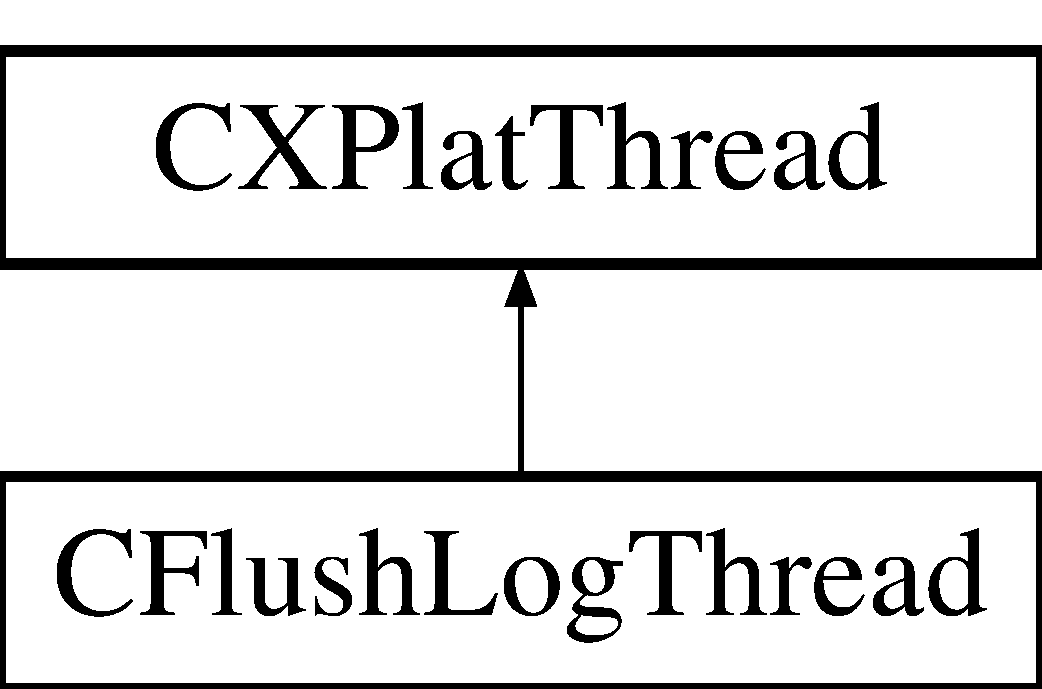
\includegraphics[height=2.000000cm]{class_c_flush_log_thread}
\end{center}
\end{figure}
\subsection*{\-Public \-Member \-Functions}
\begin{DoxyCompactItemize}
\item 
\hyperlink{class_c_flush_log_thread_a583363a6e1af4601901d406254791ce5}{\-C\-Flush\-Log\-Thread} ()
\item 
virtual \hyperlink{class_c_flush_log_thread_ab91f0358dc76376160e69c835d41a7f7}{$\sim$\-C\-Flush\-Log\-Thread} ()
\item 
\hyperlink{_cpclient_8h_a6464f7480a0fd0ee170cba12b2c0497f}{void} \hyperlink{class_c_flush_log_thread_af9c29274e8b380a87d9e5d90e57e72ce}{\-Stop\-Thread} ()
\end{DoxyCompactItemize}
\subsection*{\-Protected \-Member \-Functions}
\begin{DoxyCompactItemize}
\item 
virtual unsigned \hyperlink{class_c_flush_log_thread_a05b87f7942b745eb6a0f128b564cc9f6}{\-Worker\-Function} (\hyperlink{_cpclient_8h_a6464f7480a0fd0ee170cba12b2c0497f}{void} $\ast$p\-Param)
\begin{DoxyCompactList}\small\item\em \-Called by \-Win32\-Thread to start work in object context. \end{DoxyCompactList}\end{DoxyCompactItemize}
\subsection*{\-Protected \-Attributes}
\begin{DoxyCompactItemize}
\item 
\hyperlink{class_c_x_plat_event}{\-C\-X\-Plat\-Event} \hyperlink{class_c_flush_log_thread_a11b22bac683093063d370dce191cfe21}{c\-Stop\-Event}
\end{DoxyCompactItemize}


\subsection{\-Detailed \-Description}
\hyperlink{_c_flush_log_thread_8h}{\-C\-Flush\-Log\-Thread.\-h}\-: interface for the \hyperlink{class_c_flush_log_thread}{\-C\-Flush\-Log\-Thread} class. 

\-\_\-\-M\-S\-C\-\_\-\-V\-E\-R $>$ 1000 \-Used by \hyperlink{class_c_logging}{\-C\-Logging} to flush the buffer at regular intervals 

\-Definition at line 29 of file \-C\-Flush\-Log\-Thread.\-h.



\subsection{\-Constructor \& \-Destructor \-Documentation}
\hypertarget{class_c_flush_log_thread_a583363a6e1af4601901d406254791ce5}{\index{\-C\-Flush\-Log\-Thread@{\-C\-Flush\-Log\-Thread}!\-C\-Flush\-Log\-Thread@{\-C\-Flush\-Log\-Thread}}
\index{\-C\-Flush\-Log\-Thread@{\-C\-Flush\-Log\-Thread}!CFlushLogThread@{\-C\-Flush\-Log\-Thread}}
\subsubsection[{\-C\-Flush\-Log\-Thread}]{\setlength{\rightskip}{0pt plus 5cm}{\bf \-C\-Flush\-Log\-Thread\-::\-C\-Flush\-Log\-Thread} (
\begin{DoxyParamCaption}
{}
\end{DoxyParamCaption}
)}}\label{class_c_flush_log_thread_a583363a6e1af4601901d406254791ce5}


\-Definition at line 27 of file \-C\-Flush\-Log\-Thread.\-cpp.

\hypertarget{class_c_flush_log_thread_ab91f0358dc76376160e69c835d41a7f7}{\index{\-C\-Flush\-Log\-Thread@{\-C\-Flush\-Log\-Thread}!$\sim$\-C\-Flush\-Log\-Thread@{$\sim$\-C\-Flush\-Log\-Thread}}
\index{$\sim$\-C\-Flush\-Log\-Thread@{$\sim$\-C\-Flush\-Log\-Thread}!CFlushLogThread@{\-C\-Flush\-Log\-Thread}}
\subsubsection[{$\sim$\-C\-Flush\-Log\-Thread}]{\setlength{\rightskip}{0pt plus 5cm}{\bf \-C\-Flush\-Log\-Thread\-::$\sim$\-C\-Flush\-Log\-Thread} (
\begin{DoxyParamCaption}
{}
\end{DoxyParamCaption}
)\hspace{0.3cm}{\ttfamily  \mbox{[}virtual\mbox{]}}}}\label{class_c_flush_log_thread_ab91f0358dc76376160e69c835d41a7f7}


\-Definition at line 31 of file \-C\-Flush\-Log\-Thread.\-cpp.



\subsection{\-Member \-Function \-Documentation}
\hypertarget{class_c_flush_log_thread_af9c29274e8b380a87d9e5d90e57e72ce}{\index{\-C\-Flush\-Log\-Thread@{\-C\-Flush\-Log\-Thread}!\-Stop\-Thread@{\-Stop\-Thread}}
\index{\-Stop\-Thread@{\-Stop\-Thread}!CFlushLogThread@{\-C\-Flush\-Log\-Thread}}
\subsubsection[{\-Stop\-Thread}]{\setlength{\rightskip}{0pt plus 5cm}{\bf void} {\bf \-C\-Flush\-Log\-Thread\-::\-Stop\-Thread} (
\begin{DoxyParamCaption}
{}
\end{DoxyParamCaption}
)}}\label{class_c_flush_log_thread_af9c29274e8b380a87d9e5d90e57e72ce}


\-Definition at line 69 of file \-C\-Flush\-Log\-Thread.\-cpp.

\hypertarget{class_c_flush_log_thread_a05b87f7942b745eb6a0f128b564cc9f6}{\index{\-C\-Flush\-Log\-Thread@{\-C\-Flush\-Log\-Thread}!\-Worker\-Function@{\-Worker\-Function}}
\index{\-Worker\-Function@{\-Worker\-Function}!CFlushLogThread@{\-C\-Flush\-Log\-Thread}}
\subsubsection[{\-Worker\-Function}]{\setlength{\rightskip}{0pt plus 5cm}unsigned {\bf \-C\-Flush\-Log\-Thread\-::\-Worker\-Function} (
\begin{DoxyParamCaption}
\item[{{\bf void} $\ast$}]{p\-Param}
\end{DoxyParamCaption}
)\hspace{0.3cm}{\ttfamily  \mbox{[}protected, virtual\mbox{]}}}}\label{class_c_flush_log_thread_a05b87f7942b745eb6a0f128b564cc9f6}


\-Called by \-Win32\-Thread to start work in object context. 



\-Implements \hyperlink{class_c_x_plat_thread_af8a15900817f9673c6fd8e85cdedf27d}{\-C\-X\-Plat\-Thread}.



\-Definition at line 39 of file \-C\-Flush\-Log\-Thread.\-cpp.



\subsection{\-Member \-Data \-Documentation}
\hypertarget{class_c_flush_log_thread_a11b22bac683093063d370dce191cfe21}{\index{\-C\-Flush\-Log\-Thread@{\-C\-Flush\-Log\-Thread}!c\-Stop\-Event@{c\-Stop\-Event}}
\index{c\-Stop\-Event@{c\-Stop\-Event}!CFlushLogThread@{\-C\-Flush\-Log\-Thread}}
\subsubsection[{c\-Stop\-Event}]{\setlength{\rightskip}{0pt plus 5cm}{\bf \-C\-X\-Plat\-Event} {\bf \-C\-Flush\-Log\-Thread\-::c\-Stop\-Event}\hspace{0.3cm}{\ttfamily  \mbox{[}protected\mbox{]}}}}\label{class_c_flush_log_thread_a11b22bac683093063d370dce191cfe21}


\-Definition at line 42 of file \-C\-Flush\-Log\-Thread.\-h.



\-The documentation for this class was generated from the following files\-:\begin{DoxyCompactItemize}
\item 
common/\hyperlink{_c_flush_log_thread_8h}{\-C\-Flush\-Log\-Thread.\-h}\item 
common/\hyperlink{_c_flush_log_thread_8cpp}{\-C\-Flush\-Log\-Thread.\-cpp}\end{DoxyCompactItemize}

\hypertarget{class_c_g_i_c_plus_plus}{\section{\-C\-G\-I\-C\-Plus\-Plus \-Class \-Reference}
\label{class_c_g_i_c_plus_plus}\index{\-C\-G\-I\-C\-Plus\-Plus@{\-C\-G\-I\-C\-Plus\-Plus}}
}


\-Wrapper to simplify \-C++ creation of \-C\-G\-I programs.  




{\ttfamily \#include $<$\-C\-G\-I\-C\-Plus\-Plus.\-h$>$}

\-Inheritance diagram for \-C\-G\-I\-C\-Plus\-Plus\-:\begin{figure}[H]
\begin{center}
\leavevmode
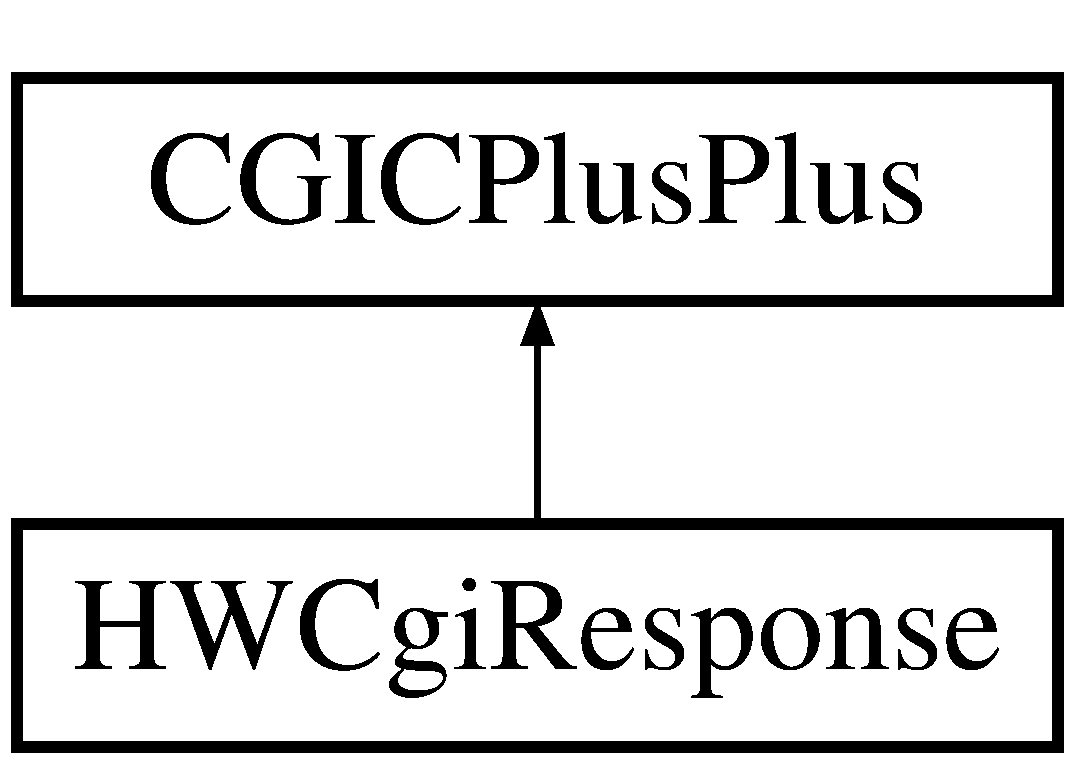
\includegraphics[height=2.000000cm]{class_c_g_i_c_plus_plus}
\end{center}
\end{figure}
\subsection*{\-Public \-Member \-Functions}
\begin{DoxyCompactItemize}
\item 
\hyperlink{class_c_g_i_c_plus_plus_a9fca234b02a37170066c13e139cf304c}{\-C\-G\-I\-C\-Plus\-Plus} ()
\item 
virtual \hyperlink{class_c_g_i_c_plus_plus_ad2053bb2b45984aa8ea326b3e1baa805}{$\sim$\-C\-G\-I\-C\-Plus\-Plus} ()
\item 
int \hyperlink{class_c_g_i_c_plus_plus_a53a8d30eb76e65d6da90c804dea755dc}{\-Get\-Variable\-Count} ()
\begin{DoxyCompactList}\small\item\em \-Get the number of variables that we found. \end{DoxyCompactList}\item 
const char $\ast$ \hyperlink{class_c_g_i_c_plus_plus_a202b1ce20242b0556003c8771bd32563}{\-Get\-Environment\-Value} (const char $\ast$p\-Variable)
\begin{DoxyCompactList}\small\item\em \-Return the value of an environment variable. \end{DoxyCompactList}\item 
const char $\ast$ \hyperlink{class_c_g_i_c_plus_plus_a1789fec84be38c186f166011368c9beb}{\-Get\-C\-G\-I\-Variable} (const char $\ast$p\-Key)
\begin{DoxyCompactList}\small\item\em \-Get the value of a \-C\-G\-I variable. \end{DoxyCompactList}\item 
\hyperlink{_cpclient_8h_a6464f7480a0fd0ee170cba12b2c0497f}{void} \hyperlink{class_c_g_i_c_plus_plus_a715711e9f674fff734a64120c5600ab2}{\-Set\-Response\-Mime\-Type} (const char $\ast$p\-Mime\-Type)
\begin{DoxyCompactList}\small\item\em \-Add response header. \end{DoxyCompactList}\item 
\hyperlink{_cpclient_8h_a6464f7480a0fd0ee170cba12b2c0497f}{void} \hyperlink{class_c_g_i_c_plus_plus_ac8ca7c0557a670b8232ff3d8a6ed6280}{\-Add\-To\-Header} (const char $\ast$p\-Content)
\begin{DoxyCompactList}\small\item\em \-Add to header. \end{DoxyCompactList}\item 
\hyperlink{_cpclient_8h_a6464f7480a0fd0ee170cba12b2c0497f}{void} \hyperlink{class_c_g_i_c_plus_plus_afe65eb134d2a50350cd84aa5dbf93a77}{\-Add\-To\-Response} (const char $\ast$p\-Content)
\begin{DoxyCompactList}\small\item\em \-Add to response. \end{DoxyCompactList}\item 
\hyperlink{_cpclient_8h_a6464f7480a0fd0ee170cba12b2c0497f}{void} \hyperlink{class_c_g_i_c_plus_plus_aa4d752cb80937e653cdea73ee7761d6d}{\-Output\-Response} ()
\begin{DoxyCompactList}\small\item\em \-Output the response. \end{DoxyCompactList}\item 
\hyperlink{_cpclient_8h_a6464f7480a0fd0ee170cba12b2c0497f}{void} \hyperlink{class_c_g_i_c_plus_plus_a526b66e47624baadbf21e43004907256}{\-Process\-Request} ()
\begin{DoxyCompactList}\small\item\em \-This function will direct to one of the following 4 function based on the http verb. \end{DoxyCompactList}\item 
virtual \hyperlink{_cpclient_8h_a6464f7480a0fd0ee170cba12b2c0497f}{void} \hyperlink{class_c_g_i_c_plus_plus_a9769c9cb4d5d9245257816ff39891764}{\-Process\-H\-E\-A\-D\-Request} ()
\begin{DoxyCompactList}\small\item\em \-You must implement this method in a derived class. \end{DoxyCompactList}\item 
virtual \hyperlink{_cpclient_8h_a6464f7480a0fd0ee170cba12b2c0497f}{void} \hyperlink{class_c_g_i_c_plus_plus_a378fb441bed59d816017d7e1ea6296f2}{\-Process\-G\-E\-T\-Request} ()
\begin{DoxyCompactList}\small\item\em \-You must implement this method in a derived class. \end{DoxyCompactList}\item 
virtual \hyperlink{_cpclient_8h_a6464f7480a0fd0ee170cba12b2c0497f}{void} \hyperlink{class_c_g_i_c_plus_plus_a2f2776ae8909abdf3769c84415d64952}{\-Process\-P\-O\-S\-T\-Request} ()
\begin{DoxyCompactList}\small\item\em \-You must implement this method in a derived class. \end{DoxyCompactList}\item 
virtual \hyperlink{_cpclient_8h_a6464f7480a0fd0ee170cba12b2c0497f}{void} \hyperlink{class_c_g_i_c_plus_plus_a86c58f739d561752f70330f321a5351b}{\-Process\-D\-E\-L\-E\-T\-E\-Request} ()
\begin{DoxyCompactList}\small\item\em \-You must implement this method in a derived class. \end{DoxyCompactList}\item 
virtual \hyperlink{_cpclient_8h_a6464f7480a0fd0ee170cba12b2c0497f}{void} \hyperlink{class_c_g_i_c_plus_plus_af903fb45e8aea8b38d2d5f49b59c8e47}{\-Process\-P\-U\-T\-Request} ()
\begin{DoxyCompactList}\small\item\em \-You must implement this method in a derived class. \end{DoxyCompactList}\item 
\hyperlink{class_c_g_i_c_plus_plus_a9fca234b02a37170066c13e139cf304c}{\-C\-G\-I\-C\-Plus\-Plus} ()
\item 
virtual \hyperlink{class_c_g_i_c_plus_plus_a908b30bdf28a2050775727046e5db7b4}{$\sim$\-C\-G\-I\-C\-Plus\-Plus} ()
\item 
int \hyperlink{class_c_g_i_c_plus_plus_a53a8d30eb76e65d6da90c804dea755dc}{\-Get\-Variable\-Count} ()
\begin{DoxyCompactList}\small\item\em \-Get the number of variables that we found. \end{DoxyCompactList}\item 
const char $\ast$ \hyperlink{class_c_g_i_c_plus_plus_a02f0d93c958335a894ab723ca8491ac0}{\-Get\-Environment\-Value} (const char $\ast$p\-Variable)
\begin{DoxyCompactList}\small\item\em \-Return the value of an environment variable. \end{DoxyCompactList}\item 
const char $\ast$ \hyperlink{class_c_g_i_c_plus_plus_a9ebd4e6761873133a6d1ca312a63bf33}{\-Get\-C\-G\-I\-Variable} (const char $\ast$p\-Key)
\begin{DoxyCompactList}\small\item\em \-Get the value of a \-C\-G\-I variable. \end{DoxyCompactList}\item 
\hyperlink{_cpclient_8h_a6464f7480a0fd0ee170cba12b2c0497f}{void} \hyperlink{class_c_g_i_c_plus_plus_a715711e9f674fff734a64120c5600ab2}{\-Set\-Response\-Mime\-Type} (const char $\ast$p\-Mime\-Type)
\begin{DoxyCompactList}\small\item\em \-Add response header. \end{DoxyCompactList}\item 
\hyperlink{_cpclient_8h_a6464f7480a0fd0ee170cba12b2c0497f}{void} \hyperlink{class_c_g_i_c_plus_plus_ac8ca7c0557a670b8232ff3d8a6ed6280}{\-Add\-To\-Header} (const char $\ast$p\-Content)
\begin{DoxyCompactList}\small\item\em \-Add to header. \end{DoxyCompactList}\item 
\hyperlink{_cpclient_8h_a6464f7480a0fd0ee170cba12b2c0497f}{void} \hyperlink{class_c_g_i_c_plus_plus_afe65eb134d2a50350cd84aa5dbf93a77}{\-Add\-To\-Response} (const char $\ast$p\-Content)
\begin{DoxyCompactList}\small\item\em \-Add to response. \end{DoxyCompactList}\item 
\hyperlink{_cpclient_8h_a6464f7480a0fd0ee170cba12b2c0497f}{void} \hyperlink{class_c_g_i_c_plus_plus_aa4d752cb80937e653cdea73ee7761d6d}{\-Output\-Response} ()
\begin{DoxyCompactList}\small\item\em \-Output the response. \end{DoxyCompactList}\item 
\hyperlink{_cpclient_8h_a6464f7480a0fd0ee170cba12b2c0497f}{void} \hyperlink{class_c_g_i_c_plus_plus_a526b66e47624baadbf21e43004907256}{\-Process\-Request} ()
\begin{DoxyCompactList}\small\item\em \-This function will direct to one of the following 4 function based on the http verb. \end{DoxyCompactList}\item 
virtual \hyperlink{_cpclient_8h_a6464f7480a0fd0ee170cba12b2c0497f}{void} \hyperlink{class_c_g_i_c_plus_plus_a9769c9cb4d5d9245257816ff39891764}{\-Process\-H\-E\-A\-D\-Request} ()
\begin{DoxyCompactList}\small\item\em \-You must implement this method in a derived class. \end{DoxyCompactList}\item 
virtual \hyperlink{_cpclient_8h_a6464f7480a0fd0ee170cba12b2c0497f}{void} \hyperlink{class_c_g_i_c_plus_plus_a378fb441bed59d816017d7e1ea6296f2}{\-Process\-G\-E\-T\-Request} ()
\begin{DoxyCompactList}\small\item\em \-You must implement this method in a derived class. \end{DoxyCompactList}\item 
virtual \hyperlink{_cpclient_8h_a6464f7480a0fd0ee170cba12b2c0497f}{void} \hyperlink{class_c_g_i_c_plus_plus_a2f2776ae8909abdf3769c84415d64952}{\-Process\-P\-O\-S\-T\-Request} ()
\begin{DoxyCompactList}\small\item\em \-You must implement this method in a derived class. \end{DoxyCompactList}\item 
virtual \hyperlink{_cpclient_8h_a6464f7480a0fd0ee170cba12b2c0497f}{void} \hyperlink{class_c_g_i_c_plus_plus_a86c58f739d561752f70330f321a5351b}{\-Process\-D\-E\-L\-E\-T\-E\-Request} ()
\begin{DoxyCompactList}\small\item\em \-You must implement this method in a derived class. \end{DoxyCompactList}\item 
virtual \hyperlink{_cpclient_8h_a6464f7480a0fd0ee170cba12b2c0497f}{void} \hyperlink{class_c_g_i_c_plus_plus_af903fb45e8aea8b38d2d5f49b59c8e47}{\-Process\-P\-U\-T\-Request} ()
\begin{DoxyCompactList}\small\item\em \-You must implement this method in a derived class. \end{DoxyCompactList}\end{DoxyCompactItemize}
\subsection*{\-Protected \-Member \-Functions}
\begin{DoxyCompactItemize}
\item 
char \hyperlink{class_c_g_i_c_plus_plus_a52641ea9cc0d1e4862e8d7c488f8a81b}{x2c} (char $\ast$what)
\begin{DoxyCompactList}\small\item\em \-Convert a two-\/char hex string into a char. \end{DoxyCompactList}\item 
\hyperlink{_cpclient_8h_a6464f7480a0fd0ee170cba12b2c0497f}{void} \hyperlink{class_c_g_i_c_plus_plus_a3f269cbf0c5a66de7fa1fdadf5a4bb26}{unescape\-\_\-url} (char $\ast$url)
\begin{DoxyCompactList}\small\item\em \-Reduce any xx escape sequences to the characters they represent. \end{DoxyCompactList}\item 
bool \hyperlink{class_c_g_i_c_plus_plus_a12301e8929d6ef34d219152b442bdb06}{\-Parse\-Request} ()
\begin{DoxyCompactList}\small\item\em \-Parse request. \end{DoxyCompactList}\item 
char \hyperlink{class_c_g_i_c_plus_plus_a52641ea9cc0d1e4862e8d7c488f8a81b}{x2c} (char $\ast$what)
\begin{DoxyCompactList}\small\item\em \-Convert a two-\/char hex string into a char. \end{DoxyCompactList}\item 
\hyperlink{_cpclient_8h_a6464f7480a0fd0ee170cba12b2c0497f}{void} \hyperlink{class_c_g_i_c_plus_plus_a3f269cbf0c5a66de7fa1fdadf5a4bb26}{unescape\-\_\-url} (char $\ast$url)
\begin{DoxyCompactList}\small\item\em \-Reduce any xx escape sequences to the characters they represent. \end{DoxyCompactList}\item 
bool \hyperlink{class_c_g_i_c_plus_plus_a12301e8929d6ef34d219152b442bdb06}{\-Parse\-Request} ()
\begin{DoxyCompactList}\small\item\em \-Parse request. \end{DoxyCompactList}\end{DoxyCompactItemize}
\subsection*{\-Protected \-Attributes}
\begin{DoxyCompactItemize}
\item 
\hyperlink{_c_g_i_c_plus_plus_8h_a4dec09a80640f7bd2995d58d468076c8}{\-M\-A\-P\-\_\-\-C\-G\-I\-\_\-\-V\-A\-L\-U\-E\-S} \hyperlink{class_c_g_i_c_plus_plus_ab9e93ef40ff2c7a9e5281148814793b3}{m\-Cgi\-Map}
\item 
\hyperlink{_c_g_i_c_plus_plus_8h_af7e8a42feb278a380f7c0926876e028d}{\-C\-V\-Iter} \hyperlink{class_c_g_i_c_plus_plus_a7af1db5a11ab0700b407c22403e7435d}{c\-Iter}
\item 
string \hyperlink{class_c_g_i_c_plus_plus_af2082316224a148d5efb74b7567eaf45}{s\-Response}
\item 
string \hyperlink{class_c_g_i_c_plus_plus_af469f49b966f4c8609c048115eab5a9b}{s\-Header}
\item 
string \hyperlink{class_c_g_i_c_plus_plus_abf093cd7afffe33ae0d514a7cf38ea24}{s\-Env\-Var}
\end{DoxyCompactItemize}


\subsection{\-Detailed \-Description}
\-Wrapper to simplify \-C++ creation of \-C\-G\-I programs. 

\-Definition at line 48 of file \-C\-G\-I\-C\-Plus\-Plus.\-h.



\subsection{\-Constructor \& \-Destructor \-Documentation}
\hypertarget{class_c_g_i_c_plus_plus_a9fca234b02a37170066c13e139cf304c}{\index{\-C\-G\-I\-C\-Plus\-Plus@{\-C\-G\-I\-C\-Plus\-Plus}!\-C\-G\-I\-C\-Plus\-Plus@{\-C\-G\-I\-C\-Plus\-Plus}}
\index{\-C\-G\-I\-C\-Plus\-Plus@{\-C\-G\-I\-C\-Plus\-Plus}!CGICPlusPlus@{\-C\-G\-I\-C\-Plus\-Plus}}
\subsubsection[{\-C\-G\-I\-C\-Plus\-Plus}]{\setlength{\rightskip}{0pt plus 5cm}{\bf \-C\-G\-I\-C\-Plus\-Plus\-::\-C\-G\-I\-C\-Plus\-Plus} (
\begin{DoxyParamCaption}
{}
\end{DoxyParamCaption}
)}}\label{class_c_g_i_c_plus_plus_a9fca234b02a37170066c13e139cf304c}


\-Definition at line 25 of file \-C\-G\-I\-C\-Plus\-Plus.\-cpp.

\hypertarget{class_c_g_i_c_plus_plus_ad2053bb2b45984aa8ea326b3e1baa805}{\index{\-C\-G\-I\-C\-Plus\-Plus@{\-C\-G\-I\-C\-Plus\-Plus}!$\sim$\-C\-G\-I\-C\-Plus\-Plus@{$\sim$\-C\-G\-I\-C\-Plus\-Plus}}
\index{$\sim$\-C\-G\-I\-C\-Plus\-Plus@{$\sim$\-C\-G\-I\-C\-Plus\-Plus}!CGICPlusPlus@{\-C\-G\-I\-C\-Plus\-Plus}}
\subsubsection[{$\sim$\-C\-G\-I\-C\-Plus\-Plus}]{\setlength{\rightskip}{0pt plus 5cm}{\bf \-C\-G\-I\-C\-Plus\-Plus\-::$\sim$\-C\-G\-I\-C\-Plus\-Plus} (
\begin{DoxyParamCaption}
{}
\end{DoxyParamCaption}
)\hspace{0.3cm}{\ttfamily  \mbox{[}virtual\mbox{]}}}}\label{class_c_g_i_c_plus_plus_ad2053bb2b45984aa8ea326b3e1baa805}


\-Definition at line 39 of file \-C\-G\-I\-C\-Plus\-Plus.\-cpp.

\hypertarget{class_c_g_i_c_plus_plus_a9fca234b02a37170066c13e139cf304c}{\index{\-C\-G\-I\-C\-Plus\-Plus@{\-C\-G\-I\-C\-Plus\-Plus}!\-C\-G\-I\-C\-Plus\-Plus@{\-C\-G\-I\-C\-Plus\-Plus}}
\index{\-C\-G\-I\-C\-Plus\-Plus@{\-C\-G\-I\-C\-Plus\-Plus}!CGICPlusPlus@{\-C\-G\-I\-C\-Plus\-Plus}}
\subsubsection[{\-C\-G\-I\-C\-Plus\-Plus}]{\setlength{\rightskip}{0pt plus 5cm}{\bf \-C\-G\-I\-C\-Plus\-Plus\-::\-C\-G\-I\-C\-Plus\-Plus} (
\begin{DoxyParamCaption}
{}
\end{DoxyParamCaption}
)}}\label{class_c_g_i_c_plus_plus_a9fca234b02a37170066c13e139cf304c}
\hypertarget{class_c_g_i_c_plus_plus_a908b30bdf28a2050775727046e5db7b4}{\index{\-C\-G\-I\-C\-Plus\-Plus@{\-C\-G\-I\-C\-Plus\-Plus}!$\sim$\-C\-G\-I\-C\-Plus\-Plus@{$\sim$\-C\-G\-I\-C\-Plus\-Plus}}
\index{$\sim$\-C\-G\-I\-C\-Plus\-Plus@{$\sim$\-C\-G\-I\-C\-Plus\-Plus}!CGICPlusPlus@{\-C\-G\-I\-C\-Plus\-Plus}}
\subsubsection[{$\sim$\-C\-G\-I\-C\-Plus\-Plus}]{\setlength{\rightskip}{0pt plus 5cm}virtual {\bf \-C\-G\-I\-C\-Plus\-Plus\-::$\sim$\-C\-G\-I\-C\-Plus\-Plus} (
\begin{DoxyParamCaption}
{}
\end{DoxyParamCaption}
)\hspace{0.3cm}{\ttfamily  \mbox{[}virtual\mbox{]}}}}\label{class_c_g_i_c_plus_plus_a908b30bdf28a2050775727046e5db7b4}


\subsection{\-Member \-Function \-Documentation}
\hypertarget{class_c_g_i_c_plus_plus_ac8ca7c0557a670b8232ff3d8a6ed6280}{\index{\-C\-G\-I\-C\-Plus\-Plus@{\-C\-G\-I\-C\-Plus\-Plus}!\-Add\-To\-Header@{\-Add\-To\-Header}}
\index{\-Add\-To\-Header@{\-Add\-To\-Header}!CGICPlusPlus@{\-C\-G\-I\-C\-Plus\-Plus}}
\subsubsection[{\-Add\-To\-Header}]{\setlength{\rightskip}{0pt plus 5cm}{\bf void} {\bf \-C\-G\-I\-C\-Plus\-Plus\-::\-Add\-To\-Header} (
\begin{DoxyParamCaption}
\item[{const char $\ast$}]{p\-Content}
\end{DoxyParamCaption}
)}}\label{class_c_g_i_c_plus_plus_ac8ca7c0557a670b8232ff3d8a6ed6280}


\-Add to header. 



\-Definition at line 145 of file \-C\-G\-I\-C\-Plus\-Plus.\-cpp.

\hypertarget{class_c_g_i_c_plus_plus_ac8ca7c0557a670b8232ff3d8a6ed6280}{\index{\-C\-G\-I\-C\-Plus\-Plus@{\-C\-G\-I\-C\-Plus\-Plus}!\-Add\-To\-Header@{\-Add\-To\-Header}}
\index{\-Add\-To\-Header@{\-Add\-To\-Header}!CGICPlusPlus@{\-C\-G\-I\-C\-Plus\-Plus}}
\subsubsection[{\-Add\-To\-Header}]{\setlength{\rightskip}{0pt plus 5cm}{\bf void} {\bf \-C\-G\-I\-C\-Plus\-Plus\-::\-Add\-To\-Header} (
\begin{DoxyParamCaption}
\item[{const char $\ast$}]{p\-Content}
\end{DoxyParamCaption}
)}}\label{class_c_g_i_c_plus_plus_ac8ca7c0557a670b8232ff3d8a6ed6280}


\-Add to header. 

\hypertarget{class_c_g_i_c_plus_plus_afe65eb134d2a50350cd84aa5dbf93a77}{\index{\-C\-G\-I\-C\-Plus\-Plus@{\-C\-G\-I\-C\-Plus\-Plus}!\-Add\-To\-Response@{\-Add\-To\-Response}}
\index{\-Add\-To\-Response@{\-Add\-To\-Response}!CGICPlusPlus@{\-C\-G\-I\-C\-Plus\-Plus}}
\subsubsection[{\-Add\-To\-Response}]{\setlength{\rightskip}{0pt plus 5cm}{\bf void} {\bf \-C\-G\-I\-C\-Plus\-Plus\-::\-Add\-To\-Response} (
\begin{DoxyParamCaption}
\item[{const char $\ast$}]{p\-Content}
\end{DoxyParamCaption}
)}}\label{class_c_g_i_c_plus_plus_afe65eb134d2a50350cd84aa5dbf93a77}


\-Add to response. 

\hypertarget{class_c_g_i_c_plus_plus_afe65eb134d2a50350cd84aa5dbf93a77}{\index{\-C\-G\-I\-C\-Plus\-Plus@{\-C\-G\-I\-C\-Plus\-Plus}!\-Add\-To\-Response@{\-Add\-To\-Response}}
\index{\-Add\-To\-Response@{\-Add\-To\-Response}!CGICPlusPlus@{\-C\-G\-I\-C\-Plus\-Plus}}
\subsubsection[{\-Add\-To\-Response}]{\setlength{\rightskip}{0pt plus 5cm}{\bf void} {\bf \-C\-G\-I\-C\-Plus\-Plus\-::\-Add\-To\-Response} (
\begin{DoxyParamCaption}
\item[{const char $\ast$}]{p\-Content}
\end{DoxyParamCaption}
)}}\label{class_c_g_i_c_plus_plus_afe65eb134d2a50350cd84aa5dbf93a77}


\-Add to response. 



\-Definition at line 139 of file \-C\-G\-I\-C\-Plus\-Plus.\-cpp.

\hypertarget{class_c_g_i_c_plus_plus_a9ebd4e6761873133a6d1ca312a63bf33}{\index{\-C\-G\-I\-C\-Plus\-Plus@{\-C\-G\-I\-C\-Plus\-Plus}!\-Get\-C\-G\-I\-Variable@{\-Get\-C\-G\-I\-Variable}}
\index{\-Get\-C\-G\-I\-Variable@{\-Get\-C\-G\-I\-Variable}!CGICPlusPlus@{\-C\-G\-I\-C\-Plus\-Plus}}
\subsubsection[{\-Get\-C\-G\-I\-Variable}]{\setlength{\rightskip}{0pt plus 5cm}const char$\ast$ {\bf \-C\-G\-I\-C\-Plus\-Plus\-::\-Get\-C\-G\-I\-Variable} (
\begin{DoxyParamCaption}
\item[{const char $\ast$}]{p\-Key}
\end{DoxyParamCaption}
)}}\label{class_c_g_i_c_plus_plus_a9ebd4e6761873133a6d1ca312a63bf33}


\-Get the value of a \-C\-G\-I variable. 

\hypertarget{class_c_g_i_c_plus_plus_a1789fec84be38c186f166011368c9beb}{\index{\-C\-G\-I\-C\-Plus\-Plus@{\-C\-G\-I\-C\-Plus\-Plus}!\-Get\-C\-G\-I\-Variable@{\-Get\-C\-G\-I\-Variable}}
\index{\-Get\-C\-G\-I\-Variable@{\-Get\-C\-G\-I\-Variable}!CGICPlusPlus@{\-C\-G\-I\-C\-Plus\-Plus}}
\subsubsection[{\-Get\-C\-G\-I\-Variable}]{\setlength{\rightskip}{0pt plus 5cm}const char $\ast$ {\bf \-C\-G\-I\-C\-Plus\-Plus\-::\-Get\-C\-G\-I\-Variable} (
\begin{DoxyParamCaption}
\item[{const char $\ast$}]{p\-Key}
\end{DoxyParamCaption}
)}}\label{class_c_g_i_c_plus_plus_a1789fec84be38c186f166011368c9beb}


\-Get the value of a \-C\-G\-I variable. 



\-Definition at line 189 of file \-C\-G\-I\-C\-Plus\-Plus.\-cpp.

\hypertarget{class_c_g_i_c_plus_plus_a02f0d93c958335a894ab723ca8491ac0}{\index{\-C\-G\-I\-C\-Plus\-Plus@{\-C\-G\-I\-C\-Plus\-Plus}!\-Get\-Environment\-Value@{\-Get\-Environment\-Value}}
\index{\-Get\-Environment\-Value@{\-Get\-Environment\-Value}!CGICPlusPlus@{\-C\-G\-I\-C\-Plus\-Plus}}
\subsubsection[{\-Get\-Environment\-Value}]{\setlength{\rightskip}{0pt plus 5cm}const char$\ast$ {\bf \-C\-G\-I\-C\-Plus\-Plus\-::\-Get\-Environment\-Value} (
\begin{DoxyParamCaption}
\item[{const char $\ast$}]{p\-Variable}
\end{DoxyParamCaption}
)}}\label{class_c_g_i_c_plus_plus_a02f0d93c958335a894ab723ca8491ac0}


\-Return the value of an environment variable. 

\hypertarget{class_c_g_i_c_plus_plus_a202b1ce20242b0556003c8771bd32563}{\index{\-C\-G\-I\-C\-Plus\-Plus@{\-C\-G\-I\-C\-Plus\-Plus}!\-Get\-Environment\-Value@{\-Get\-Environment\-Value}}
\index{\-Get\-Environment\-Value@{\-Get\-Environment\-Value}!CGICPlusPlus@{\-C\-G\-I\-C\-Plus\-Plus}}
\subsubsection[{\-Get\-Environment\-Value}]{\setlength{\rightskip}{0pt plus 5cm}const char $\ast$ {\bf \-C\-G\-I\-C\-Plus\-Plus\-::\-Get\-Environment\-Value} (
\begin{DoxyParamCaption}
\item[{const char $\ast$}]{p\-Variable}
\end{DoxyParamCaption}
)}}\label{class_c_g_i_c_plus_plus_a202b1ce20242b0556003c8771bd32563}


\-Return the value of an environment variable. 



\-Definition at line 180 of file \-C\-G\-I\-C\-Plus\-Plus.\-cpp.

\hypertarget{class_c_g_i_c_plus_plus_a53a8d30eb76e65d6da90c804dea755dc}{\index{\-C\-G\-I\-C\-Plus\-Plus@{\-C\-G\-I\-C\-Plus\-Plus}!\-Get\-Variable\-Count@{\-Get\-Variable\-Count}}
\index{\-Get\-Variable\-Count@{\-Get\-Variable\-Count}!CGICPlusPlus@{\-C\-G\-I\-C\-Plus\-Plus}}
\subsubsection[{\-Get\-Variable\-Count}]{\setlength{\rightskip}{0pt plus 5cm}int {\bf \-C\-G\-I\-C\-Plus\-Plus\-::\-Get\-Variable\-Count} (
\begin{DoxyParamCaption}
{}
\end{DoxyParamCaption}
)}}\label{class_c_g_i_c_plus_plus_a53a8d30eb76e65d6da90c804dea755dc}


\-Get the number of variables that we found. 

\hypertarget{class_c_g_i_c_plus_plus_a53a8d30eb76e65d6da90c804dea755dc}{\index{\-C\-G\-I\-C\-Plus\-Plus@{\-C\-G\-I\-C\-Plus\-Plus}!\-Get\-Variable\-Count@{\-Get\-Variable\-Count}}
\index{\-Get\-Variable\-Count@{\-Get\-Variable\-Count}!CGICPlusPlus@{\-C\-G\-I\-C\-Plus\-Plus}}
\subsubsection[{\-Get\-Variable\-Count}]{\setlength{\rightskip}{0pt plus 5cm}int {\bf \-C\-G\-I\-C\-Plus\-Plus\-::\-Get\-Variable\-Count} (
\begin{DoxyParamCaption}
{}
\end{DoxyParamCaption}
)}}\label{class_c_g_i_c_plus_plus_a53a8d30eb76e65d6da90c804dea755dc}


\-Get the number of variables that we found. 



\-Definition at line 172 of file \-C\-G\-I\-C\-Plus\-Plus.\-cpp.

\hypertarget{class_c_g_i_c_plus_plus_aa4d752cb80937e653cdea73ee7761d6d}{\index{\-C\-G\-I\-C\-Plus\-Plus@{\-C\-G\-I\-C\-Plus\-Plus}!\-Output\-Response@{\-Output\-Response}}
\index{\-Output\-Response@{\-Output\-Response}!CGICPlusPlus@{\-C\-G\-I\-C\-Plus\-Plus}}
\subsubsection[{\-Output\-Response}]{\setlength{\rightskip}{0pt plus 5cm}{\bf void} {\bf \-C\-G\-I\-C\-Plus\-Plus\-::\-Output\-Response} (
\begin{DoxyParamCaption}
{}
\end{DoxyParamCaption}
)}}\label{class_c_g_i_c_plus_plus_aa4d752cb80937e653cdea73ee7761d6d}


\-Output the response. 

\hypertarget{class_c_g_i_c_plus_plus_aa4d752cb80937e653cdea73ee7761d6d}{\index{\-C\-G\-I\-C\-Plus\-Plus@{\-C\-G\-I\-C\-Plus\-Plus}!\-Output\-Response@{\-Output\-Response}}
\index{\-Output\-Response@{\-Output\-Response}!CGICPlusPlus@{\-C\-G\-I\-C\-Plus\-Plus}}
\subsubsection[{\-Output\-Response}]{\setlength{\rightskip}{0pt plus 5cm}{\bf void} {\bf \-C\-G\-I\-C\-Plus\-Plus\-::\-Output\-Response} (
\begin{DoxyParamCaption}
{}
\end{DoxyParamCaption}
)}}\label{class_c_g_i_c_plus_plus_aa4d752cb80937e653cdea73ee7761d6d}


\-Output the response. 



\-Definition at line 162 of file \-C\-G\-I\-C\-Plus\-Plus.\-cpp.

\hypertarget{class_c_g_i_c_plus_plus_a12301e8929d6ef34d219152b442bdb06}{\index{\-C\-G\-I\-C\-Plus\-Plus@{\-C\-G\-I\-C\-Plus\-Plus}!\-Parse\-Request@{\-Parse\-Request}}
\index{\-Parse\-Request@{\-Parse\-Request}!CGICPlusPlus@{\-C\-G\-I\-C\-Plus\-Plus}}
\subsubsection[{\-Parse\-Request}]{\setlength{\rightskip}{0pt plus 5cm}bool {\bf \-C\-G\-I\-C\-Plus\-Plus\-::\-Parse\-Request} (
\begin{DoxyParamCaption}
{}
\end{DoxyParamCaption}
)\hspace{0.3cm}{\ttfamily  \mbox{[}protected\mbox{]}}}}\label{class_c_g_i_c_plus_plus_a12301e8929d6ef34d219152b442bdb06}


\-Parse request. 



\-Definition at line 45 of file \-C\-G\-I\-C\-Plus\-Plus.\-cpp.

\hypertarget{class_c_g_i_c_plus_plus_a12301e8929d6ef34d219152b442bdb06}{\index{\-C\-G\-I\-C\-Plus\-Plus@{\-C\-G\-I\-C\-Plus\-Plus}!\-Parse\-Request@{\-Parse\-Request}}
\index{\-Parse\-Request@{\-Parse\-Request}!CGICPlusPlus@{\-C\-G\-I\-C\-Plus\-Plus}}
\subsubsection[{\-Parse\-Request}]{\setlength{\rightskip}{0pt plus 5cm}bool {\bf \-C\-G\-I\-C\-Plus\-Plus\-::\-Parse\-Request} (
\begin{DoxyParamCaption}
{}
\end{DoxyParamCaption}
)\hspace{0.3cm}{\ttfamily  \mbox{[}protected\mbox{]}}}}\label{class_c_g_i_c_plus_plus_a12301e8929d6ef34d219152b442bdb06}


\-Parse request. 

\hypertarget{class_c_g_i_c_plus_plus_a86c58f739d561752f70330f321a5351b}{\index{\-C\-G\-I\-C\-Plus\-Plus@{\-C\-G\-I\-C\-Plus\-Plus}!\-Process\-D\-E\-L\-E\-T\-E\-Request@{\-Process\-D\-E\-L\-E\-T\-E\-Request}}
\index{\-Process\-D\-E\-L\-E\-T\-E\-Request@{\-Process\-D\-E\-L\-E\-T\-E\-Request}!CGICPlusPlus@{\-C\-G\-I\-C\-Plus\-Plus}}
\subsubsection[{\-Process\-D\-E\-L\-E\-T\-E\-Request}]{\setlength{\rightskip}{0pt plus 5cm}virtual {\bf void} {\bf \-C\-G\-I\-C\-Plus\-Plus\-::\-Process\-D\-E\-L\-E\-T\-E\-Request} (
\begin{DoxyParamCaption}
{}
\end{DoxyParamCaption}
)\hspace{0.3cm}{\ttfamily  \mbox{[}inline, virtual\mbox{]}}}}\label{class_c_g_i_c_plus_plus_a86c58f739d561752f70330f321a5351b}


\-You must implement this method in a derived class. 



\-Definition at line 77 of file \-C\-G\-I\-C\-Plus\-Plus.\-h.

\hypertarget{class_c_g_i_c_plus_plus_a86c58f739d561752f70330f321a5351b}{\index{\-C\-G\-I\-C\-Plus\-Plus@{\-C\-G\-I\-C\-Plus\-Plus}!\-Process\-D\-E\-L\-E\-T\-E\-Request@{\-Process\-D\-E\-L\-E\-T\-E\-Request}}
\index{\-Process\-D\-E\-L\-E\-T\-E\-Request@{\-Process\-D\-E\-L\-E\-T\-E\-Request}!CGICPlusPlus@{\-C\-G\-I\-C\-Plus\-Plus}}
\subsubsection[{\-Process\-D\-E\-L\-E\-T\-E\-Request}]{\setlength{\rightskip}{0pt plus 5cm}virtual {\bf void} {\bf \-C\-G\-I\-C\-Plus\-Plus\-::\-Process\-D\-E\-L\-E\-T\-E\-Request} (
\begin{DoxyParamCaption}
{}
\end{DoxyParamCaption}
)\hspace{0.3cm}{\ttfamily  \mbox{[}inline, virtual\mbox{]}}}}\label{class_c_g_i_c_plus_plus_a86c58f739d561752f70330f321a5351b}


\-You must implement this method in a derived class. 



\-Definition at line 77 of file \-C\-G\-I\-C\-Plus\-Plus.\-h.

\hypertarget{class_c_g_i_c_plus_plus_a378fb441bed59d816017d7e1ea6296f2}{\index{\-C\-G\-I\-C\-Plus\-Plus@{\-C\-G\-I\-C\-Plus\-Plus}!\-Process\-G\-E\-T\-Request@{\-Process\-G\-E\-T\-Request}}
\index{\-Process\-G\-E\-T\-Request@{\-Process\-G\-E\-T\-Request}!CGICPlusPlus@{\-C\-G\-I\-C\-Plus\-Plus}}
\subsubsection[{\-Process\-G\-E\-T\-Request}]{\setlength{\rightskip}{0pt plus 5cm}virtual {\bf void} {\bf \-C\-G\-I\-C\-Plus\-Plus\-::\-Process\-G\-E\-T\-Request} (
\begin{DoxyParamCaption}
{}
\end{DoxyParamCaption}
)\hspace{0.3cm}{\ttfamily  \mbox{[}inline, virtual\mbox{]}}}}\label{class_c_g_i_c_plus_plus_a378fb441bed59d816017d7e1ea6296f2}


\-You must implement this method in a derived class. 



\-Reimplemented in \hyperlink{class_h_w_cgi_response_a1a4b4b8f0f682f9dc0a9e71dd6fa2fe5}{\-H\-W\-Cgi\-Response}.



\-Definition at line 73 of file \-C\-G\-I\-C\-Plus\-Plus.\-h.

\hypertarget{class_c_g_i_c_plus_plus_a378fb441bed59d816017d7e1ea6296f2}{\index{\-C\-G\-I\-C\-Plus\-Plus@{\-C\-G\-I\-C\-Plus\-Plus}!\-Process\-G\-E\-T\-Request@{\-Process\-G\-E\-T\-Request}}
\index{\-Process\-G\-E\-T\-Request@{\-Process\-G\-E\-T\-Request}!CGICPlusPlus@{\-C\-G\-I\-C\-Plus\-Plus}}
\subsubsection[{\-Process\-G\-E\-T\-Request}]{\setlength{\rightskip}{0pt plus 5cm}virtual {\bf void} {\bf \-C\-G\-I\-C\-Plus\-Plus\-::\-Process\-G\-E\-T\-Request} (
\begin{DoxyParamCaption}
{}
\end{DoxyParamCaption}
)\hspace{0.3cm}{\ttfamily  \mbox{[}inline, virtual\mbox{]}}}}\label{class_c_g_i_c_plus_plus_a378fb441bed59d816017d7e1ea6296f2}


\-You must implement this method in a derived class. 



\-Reimplemented in \hyperlink{class_h_w_cgi_response_a1a4b4b8f0f682f9dc0a9e71dd6fa2fe5}{\-H\-W\-Cgi\-Response}.



\-Definition at line 73 of file \-C\-G\-I\-C\-Plus\-Plus.\-h.

\hypertarget{class_c_g_i_c_plus_plus_a9769c9cb4d5d9245257816ff39891764}{\index{\-C\-G\-I\-C\-Plus\-Plus@{\-C\-G\-I\-C\-Plus\-Plus}!\-Process\-H\-E\-A\-D\-Request@{\-Process\-H\-E\-A\-D\-Request}}
\index{\-Process\-H\-E\-A\-D\-Request@{\-Process\-H\-E\-A\-D\-Request}!CGICPlusPlus@{\-C\-G\-I\-C\-Plus\-Plus}}
\subsubsection[{\-Process\-H\-E\-A\-D\-Request}]{\setlength{\rightskip}{0pt plus 5cm}virtual {\bf void} {\bf \-C\-G\-I\-C\-Plus\-Plus\-::\-Process\-H\-E\-A\-D\-Request} (
\begin{DoxyParamCaption}
{}
\end{DoxyParamCaption}
)\hspace{0.3cm}{\ttfamily  \mbox{[}inline, virtual\mbox{]}}}}\label{class_c_g_i_c_plus_plus_a9769c9cb4d5d9245257816ff39891764}


\-You must implement this method in a derived class. 



\-Definition at line 71 of file \-C\-G\-I\-C\-Plus\-Plus.\-h.

\hypertarget{class_c_g_i_c_plus_plus_a9769c9cb4d5d9245257816ff39891764}{\index{\-C\-G\-I\-C\-Plus\-Plus@{\-C\-G\-I\-C\-Plus\-Plus}!\-Process\-H\-E\-A\-D\-Request@{\-Process\-H\-E\-A\-D\-Request}}
\index{\-Process\-H\-E\-A\-D\-Request@{\-Process\-H\-E\-A\-D\-Request}!CGICPlusPlus@{\-C\-G\-I\-C\-Plus\-Plus}}
\subsubsection[{\-Process\-H\-E\-A\-D\-Request}]{\setlength{\rightskip}{0pt plus 5cm}virtual {\bf void} {\bf \-C\-G\-I\-C\-Plus\-Plus\-::\-Process\-H\-E\-A\-D\-Request} (
\begin{DoxyParamCaption}
{}
\end{DoxyParamCaption}
)\hspace{0.3cm}{\ttfamily  \mbox{[}inline, virtual\mbox{]}}}}\label{class_c_g_i_c_plus_plus_a9769c9cb4d5d9245257816ff39891764}


\-You must implement this method in a derived class. 



\-Definition at line 71 of file \-C\-G\-I\-C\-Plus\-Plus.\-h.

\hypertarget{class_c_g_i_c_plus_plus_a2f2776ae8909abdf3769c84415d64952}{\index{\-C\-G\-I\-C\-Plus\-Plus@{\-C\-G\-I\-C\-Plus\-Plus}!\-Process\-P\-O\-S\-T\-Request@{\-Process\-P\-O\-S\-T\-Request}}
\index{\-Process\-P\-O\-S\-T\-Request@{\-Process\-P\-O\-S\-T\-Request}!CGICPlusPlus@{\-C\-G\-I\-C\-Plus\-Plus}}
\subsubsection[{\-Process\-P\-O\-S\-T\-Request}]{\setlength{\rightskip}{0pt plus 5cm}virtual {\bf void} {\bf \-C\-G\-I\-C\-Plus\-Plus\-::\-Process\-P\-O\-S\-T\-Request} (
\begin{DoxyParamCaption}
{}
\end{DoxyParamCaption}
)\hspace{0.3cm}{\ttfamily  \mbox{[}inline, virtual\mbox{]}}}}\label{class_c_g_i_c_plus_plus_a2f2776ae8909abdf3769c84415d64952}


\-You must implement this method in a derived class. 



\-Reimplemented in \hyperlink{class_h_w_cgi_response_aec2b369683ddd63bad010575451aaec3}{\-H\-W\-Cgi\-Response}.



\-Definition at line 75 of file \-C\-G\-I\-C\-Plus\-Plus.\-h.

\hypertarget{class_c_g_i_c_plus_plus_a2f2776ae8909abdf3769c84415d64952}{\index{\-C\-G\-I\-C\-Plus\-Plus@{\-C\-G\-I\-C\-Plus\-Plus}!\-Process\-P\-O\-S\-T\-Request@{\-Process\-P\-O\-S\-T\-Request}}
\index{\-Process\-P\-O\-S\-T\-Request@{\-Process\-P\-O\-S\-T\-Request}!CGICPlusPlus@{\-C\-G\-I\-C\-Plus\-Plus}}
\subsubsection[{\-Process\-P\-O\-S\-T\-Request}]{\setlength{\rightskip}{0pt plus 5cm}virtual {\bf void} {\bf \-C\-G\-I\-C\-Plus\-Plus\-::\-Process\-P\-O\-S\-T\-Request} (
\begin{DoxyParamCaption}
{}
\end{DoxyParamCaption}
)\hspace{0.3cm}{\ttfamily  \mbox{[}inline, virtual\mbox{]}}}}\label{class_c_g_i_c_plus_plus_a2f2776ae8909abdf3769c84415d64952}


\-You must implement this method in a derived class. 



\-Reimplemented in \hyperlink{class_h_w_cgi_response_aec2b369683ddd63bad010575451aaec3}{\-H\-W\-Cgi\-Response}.



\-Definition at line 75 of file \-C\-G\-I\-C\-Plus\-Plus.\-h.

\hypertarget{class_c_g_i_c_plus_plus_af903fb45e8aea8b38d2d5f49b59c8e47}{\index{\-C\-G\-I\-C\-Plus\-Plus@{\-C\-G\-I\-C\-Plus\-Plus}!\-Process\-P\-U\-T\-Request@{\-Process\-P\-U\-T\-Request}}
\index{\-Process\-P\-U\-T\-Request@{\-Process\-P\-U\-T\-Request}!CGICPlusPlus@{\-C\-G\-I\-C\-Plus\-Plus}}
\subsubsection[{\-Process\-P\-U\-T\-Request}]{\setlength{\rightskip}{0pt plus 5cm}virtual {\bf void} {\bf \-C\-G\-I\-C\-Plus\-Plus\-::\-Process\-P\-U\-T\-Request} (
\begin{DoxyParamCaption}
{}
\end{DoxyParamCaption}
)\hspace{0.3cm}{\ttfamily  \mbox{[}inline, virtual\mbox{]}}}}\label{class_c_g_i_c_plus_plus_af903fb45e8aea8b38d2d5f49b59c8e47}


\-You must implement this method in a derived class. 



\-Definition at line 79 of file \-C\-G\-I\-C\-Plus\-Plus.\-h.

\hypertarget{class_c_g_i_c_plus_plus_af903fb45e8aea8b38d2d5f49b59c8e47}{\index{\-C\-G\-I\-C\-Plus\-Plus@{\-C\-G\-I\-C\-Plus\-Plus}!\-Process\-P\-U\-T\-Request@{\-Process\-P\-U\-T\-Request}}
\index{\-Process\-P\-U\-T\-Request@{\-Process\-P\-U\-T\-Request}!CGICPlusPlus@{\-C\-G\-I\-C\-Plus\-Plus}}
\subsubsection[{\-Process\-P\-U\-T\-Request}]{\setlength{\rightskip}{0pt plus 5cm}virtual {\bf void} {\bf \-C\-G\-I\-C\-Plus\-Plus\-::\-Process\-P\-U\-T\-Request} (
\begin{DoxyParamCaption}
{}
\end{DoxyParamCaption}
)\hspace{0.3cm}{\ttfamily  \mbox{[}inline, virtual\mbox{]}}}}\label{class_c_g_i_c_plus_plus_af903fb45e8aea8b38d2d5f49b59c8e47}


\-You must implement this method in a derived class. 



\-Definition at line 79 of file \-C\-G\-I\-C\-Plus\-Plus.\-h.

\hypertarget{class_c_g_i_c_plus_plus_a526b66e47624baadbf21e43004907256}{\index{\-C\-G\-I\-C\-Plus\-Plus@{\-C\-G\-I\-C\-Plus\-Plus}!\-Process\-Request@{\-Process\-Request}}
\index{\-Process\-Request@{\-Process\-Request}!CGICPlusPlus@{\-C\-G\-I\-C\-Plus\-Plus}}
\subsubsection[{\-Process\-Request}]{\setlength{\rightskip}{0pt plus 5cm}{\bf void} {\bf \-C\-G\-I\-C\-Plus\-Plus\-::\-Process\-Request} (
\begin{DoxyParamCaption}
{}
\end{DoxyParamCaption}
)}}\label{class_c_g_i_c_plus_plus_a526b66e47624baadbf21e43004907256}


\-This function will direct to one of the following 4 function based on the http verb. 

\hypertarget{class_c_g_i_c_plus_plus_a526b66e47624baadbf21e43004907256}{\index{\-C\-G\-I\-C\-Plus\-Plus@{\-C\-G\-I\-C\-Plus\-Plus}!\-Process\-Request@{\-Process\-Request}}
\index{\-Process\-Request@{\-Process\-Request}!CGICPlusPlus@{\-C\-G\-I\-C\-Plus\-Plus}}
\subsubsection[{\-Process\-Request}]{\setlength{\rightskip}{0pt plus 5cm}{\bf void} {\bf \-C\-G\-I\-C\-Plus\-Plus\-::\-Process\-Request} (
\begin{DoxyParamCaption}
{}
\end{DoxyParamCaption}
)}}\label{class_c_g_i_c_plus_plus_a526b66e47624baadbf21e43004907256}


\-This function will direct to one of the following 4 function based on the http verb. 



\-Definition at line 120 of file \-C\-G\-I\-C\-Plus\-Plus.\-cpp.

\hypertarget{class_c_g_i_c_plus_plus_a715711e9f674fff734a64120c5600ab2}{\index{\-C\-G\-I\-C\-Plus\-Plus@{\-C\-G\-I\-C\-Plus\-Plus}!\-Set\-Response\-Mime\-Type@{\-Set\-Response\-Mime\-Type}}
\index{\-Set\-Response\-Mime\-Type@{\-Set\-Response\-Mime\-Type}!CGICPlusPlus@{\-C\-G\-I\-C\-Plus\-Plus}}
\subsubsection[{\-Set\-Response\-Mime\-Type}]{\setlength{\rightskip}{0pt plus 5cm}{\bf void} {\bf \-C\-G\-I\-C\-Plus\-Plus\-::\-Set\-Response\-Mime\-Type} (
\begin{DoxyParamCaption}
\item[{const char $\ast$}]{p\-Mime\-Type}
\end{DoxyParamCaption}
)}}\label{class_c_g_i_c_plus_plus_a715711e9f674fff734a64120c5600ab2}


\-Add response header. 

\hypertarget{class_c_g_i_c_plus_plus_a715711e9f674fff734a64120c5600ab2}{\index{\-C\-G\-I\-C\-Plus\-Plus@{\-C\-G\-I\-C\-Plus\-Plus}!\-Set\-Response\-Mime\-Type@{\-Set\-Response\-Mime\-Type}}
\index{\-Set\-Response\-Mime\-Type@{\-Set\-Response\-Mime\-Type}!CGICPlusPlus@{\-C\-G\-I\-C\-Plus\-Plus}}
\subsubsection[{\-Set\-Response\-Mime\-Type}]{\setlength{\rightskip}{0pt plus 5cm}{\bf void} {\bf \-C\-G\-I\-C\-Plus\-Plus\-::\-Set\-Response\-Mime\-Type} (
\begin{DoxyParamCaption}
\item[{const char $\ast$}]{p\-Mime\-Type}
\end{DoxyParamCaption}
)}}\label{class_c_g_i_c_plus_plus_a715711e9f674fff734a64120c5600ab2}


\-Add response header. 



\-Definition at line 153 of file \-C\-G\-I\-C\-Plus\-Plus.\-cpp.

\hypertarget{class_c_g_i_c_plus_plus_a3f269cbf0c5a66de7fa1fdadf5a4bb26}{\index{\-C\-G\-I\-C\-Plus\-Plus@{\-C\-G\-I\-C\-Plus\-Plus}!unescape\-\_\-url@{unescape\-\_\-url}}
\index{unescape\-\_\-url@{unescape\-\_\-url}!CGICPlusPlus@{\-C\-G\-I\-C\-Plus\-Plus}}
\subsubsection[{unescape\-\_\-url}]{\setlength{\rightskip}{0pt plus 5cm}{\bf void} {\bf \-C\-G\-I\-C\-Plus\-Plus\-::unescape\-\_\-url} (
\begin{DoxyParamCaption}
\item[{char $\ast$}]{url}
\end{DoxyParamCaption}
)\hspace{0.3cm}{\ttfamily  \mbox{[}protected\mbox{]}}}}\label{class_c_g_i_c_plus_plus_a3f269cbf0c5a66de7fa1fdadf5a4bb26}


\-Reduce any xx escape sequences to the characters they represent. 

\hypertarget{class_c_g_i_c_plus_plus_a3f269cbf0c5a66de7fa1fdadf5a4bb26}{\index{\-C\-G\-I\-C\-Plus\-Plus@{\-C\-G\-I\-C\-Plus\-Plus}!unescape\-\_\-url@{unescape\-\_\-url}}
\index{unescape\-\_\-url@{unescape\-\_\-url}!CGICPlusPlus@{\-C\-G\-I\-C\-Plus\-Plus}}
\subsubsection[{unescape\-\_\-url}]{\setlength{\rightskip}{0pt plus 5cm}{\bf void} {\bf \-C\-G\-I\-C\-Plus\-Plus\-::unescape\-\_\-url} (
\begin{DoxyParamCaption}
\item[{char $\ast$}]{url}
\end{DoxyParamCaption}
)\hspace{0.3cm}{\ttfamily  \mbox{[}protected\mbox{]}}}}\label{class_c_g_i_c_plus_plus_a3f269cbf0c5a66de7fa1fdadf5a4bb26}


\-Reduce any xx escape sequences to the characters they represent. 



\-Definition at line 213 of file \-C\-G\-I\-C\-Plus\-Plus.\-cpp.

\hypertarget{class_c_g_i_c_plus_plus_a52641ea9cc0d1e4862e8d7c488f8a81b}{\index{\-C\-G\-I\-C\-Plus\-Plus@{\-C\-G\-I\-C\-Plus\-Plus}!x2c@{x2c}}
\index{x2c@{x2c}!CGICPlusPlus@{\-C\-G\-I\-C\-Plus\-Plus}}
\subsubsection[{x2c}]{\setlength{\rightskip}{0pt plus 5cm}char {\bf \-C\-G\-I\-C\-Plus\-Plus\-::x2c} (
\begin{DoxyParamCaption}
\item[{char $\ast$}]{what}
\end{DoxyParamCaption}
)\hspace{0.3cm}{\ttfamily  \mbox{[}protected\mbox{]}}}}\label{class_c_g_i_c_plus_plus_a52641ea9cc0d1e4862e8d7c488f8a81b}


\-Convert a two-\/char hex string into a char. 

\hypertarget{class_c_g_i_c_plus_plus_a52641ea9cc0d1e4862e8d7c488f8a81b}{\index{\-C\-G\-I\-C\-Plus\-Plus@{\-C\-G\-I\-C\-Plus\-Plus}!x2c@{x2c}}
\index{x2c@{x2c}!CGICPlusPlus@{\-C\-G\-I\-C\-Plus\-Plus}}
\subsubsection[{x2c}]{\setlength{\rightskip}{0pt plus 5cm}char {\bf \-C\-G\-I\-C\-Plus\-Plus\-::x2c} (
\begin{DoxyParamCaption}
\item[{char $\ast$}]{what}
\end{DoxyParamCaption}
)\hspace{0.3cm}{\ttfamily  \mbox{[}protected\mbox{]}}}}\label{class_c_g_i_c_plus_plus_a52641ea9cc0d1e4862e8d7c488f8a81b}


\-Convert a two-\/char hex string into a char. 



\-Definition at line 200 of file \-C\-G\-I\-C\-Plus\-Plus.\-cpp.



\subsection{\-Member \-Data \-Documentation}
\hypertarget{class_c_g_i_c_plus_plus_a7af1db5a11ab0700b407c22403e7435d}{\index{\-C\-G\-I\-C\-Plus\-Plus@{\-C\-G\-I\-C\-Plus\-Plus}!c\-Iter@{c\-Iter}}
\index{c\-Iter@{c\-Iter}!CGICPlusPlus@{\-C\-G\-I\-C\-Plus\-Plus}}
\subsubsection[{c\-Iter}]{\setlength{\rightskip}{0pt plus 5cm}{\bf \-C\-V\-Iter} {\bf \-C\-G\-I\-C\-Plus\-Plus\-::c\-Iter}\hspace{0.3cm}{\ttfamily  \mbox{[}protected\mbox{]}}}}\label{class_c_g_i_c_plus_plus_a7af1db5a11ab0700b407c22403e7435d}


\-Definition at line 90 of file \-C\-G\-I\-C\-Plus\-Plus.\-h.

\hypertarget{class_c_g_i_c_plus_plus_ab9e93ef40ff2c7a9e5281148814793b3}{\index{\-C\-G\-I\-C\-Plus\-Plus@{\-C\-G\-I\-C\-Plus\-Plus}!m\-Cgi\-Map@{m\-Cgi\-Map}}
\index{m\-Cgi\-Map@{m\-Cgi\-Map}!CGICPlusPlus@{\-C\-G\-I\-C\-Plus\-Plus}}
\subsubsection[{m\-Cgi\-Map}]{\setlength{\rightskip}{0pt plus 5cm}{\bf \-M\-A\-P\-\_\-\-C\-G\-I\-\_\-\-V\-A\-L\-U\-E\-S} {\bf \-C\-G\-I\-C\-Plus\-Plus\-::m\-Cgi\-Map}\hspace{0.3cm}{\ttfamily  \mbox{[}protected\mbox{]}}}}\label{class_c_g_i_c_plus_plus_ab9e93ef40ff2c7a9e5281148814793b3}


\-Definition at line 89 of file \-C\-G\-I\-C\-Plus\-Plus.\-h.

\hypertarget{class_c_g_i_c_plus_plus_abf093cd7afffe33ae0d514a7cf38ea24}{\index{\-C\-G\-I\-C\-Plus\-Plus@{\-C\-G\-I\-C\-Plus\-Plus}!s\-Env\-Var@{s\-Env\-Var}}
\index{s\-Env\-Var@{s\-Env\-Var}!CGICPlusPlus@{\-C\-G\-I\-C\-Plus\-Plus}}
\subsubsection[{s\-Env\-Var}]{\setlength{\rightskip}{0pt plus 5cm}string {\bf \-C\-G\-I\-C\-Plus\-Plus\-::s\-Env\-Var}\hspace{0.3cm}{\ttfamily  \mbox{[}protected\mbox{]}}}}\label{class_c_g_i_c_plus_plus_abf093cd7afffe33ae0d514a7cf38ea24}


\-Definition at line 93 of file \-C\-G\-I\-C\-Plus\-Plus.\-h.

\hypertarget{class_c_g_i_c_plus_plus_af469f49b966f4c8609c048115eab5a9b}{\index{\-C\-G\-I\-C\-Plus\-Plus@{\-C\-G\-I\-C\-Plus\-Plus}!s\-Header@{s\-Header}}
\index{s\-Header@{s\-Header}!CGICPlusPlus@{\-C\-G\-I\-C\-Plus\-Plus}}
\subsubsection[{s\-Header}]{\setlength{\rightskip}{0pt plus 5cm}string {\bf \-C\-G\-I\-C\-Plus\-Plus\-::s\-Header}\hspace{0.3cm}{\ttfamily  \mbox{[}protected\mbox{]}}}}\label{class_c_g_i_c_plus_plus_af469f49b966f4c8609c048115eab5a9b}


\-Definition at line 92 of file \-C\-G\-I\-C\-Plus\-Plus.\-h.

\hypertarget{class_c_g_i_c_plus_plus_af2082316224a148d5efb74b7567eaf45}{\index{\-C\-G\-I\-C\-Plus\-Plus@{\-C\-G\-I\-C\-Plus\-Plus}!s\-Response@{s\-Response}}
\index{s\-Response@{s\-Response}!CGICPlusPlus@{\-C\-G\-I\-C\-Plus\-Plus}}
\subsubsection[{s\-Response}]{\setlength{\rightskip}{0pt plus 5cm}string {\bf \-C\-G\-I\-C\-Plus\-Plus\-::s\-Response}\hspace{0.3cm}{\ttfamily  \mbox{[}protected\mbox{]}}}}\label{class_c_g_i_c_plus_plus_af2082316224a148d5efb74b7567eaf45}


\-Definition at line 91 of file \-C\-G\-I\-C\-Plus\-Plus.\-h.



\-The documentation for this class was generated from the following files\-:\begin{DoxyCompactItemize}
\item 
common/\hyperlink{_c_g_i_c_plus_plus_8h}{\-C\-G\-I\-C\-Plus\-Plus.\-h}\item 
common/examples/\-C\-G\-Iexample/\hyperlink{examples_2_c_g_iexample_2_c_g_i_c_plus_plus_8h}{\-C\-G\-I\-C\-Plus\-Plus.\-h}\item 
common/\hyperlink{_c_g_i_c_plus_plus_8cpp}{\-C\-G\-I\-C\-Plus\-Plus.\-cpp}\item 
common/examples/\-C\-G\-Iexample/\hyperlink{examples_2_c_g_iexample_2_c_g_i_c_plus_plus_8cpp}{\-C\-G\-I\-C\-Plus\-Plus.\-cpp}\end{DoxyCompactItemize}

\hypertarget{class_check_mem_signature}{\section{\-Check\-Mem\-Signature \-Class \-Reference}
\label{class_check_mem_signature}\index{\-Check\-Mem\-Signature@{\-Check\-Mem\-Signature}}
}


{\ttfamily \#include $<$\-Check\-Mem\-Signature.\-h$>$}

\subsection*{\-Public \-Member \-Functions}
\begin{DoxyCompactItemize}
\item 
\hyperlink{class_check_mem_signature_a3cc20e6a1eb1424cc62d488562aec572}{\-Check\-Mem\-Signature} (bool b\-Mem\-Log=true)
\item 
virtual \hyperlink{class_check_mem_signature_a7c24bca0f4aadb879ce156e732a19aa3}{$\sim$\-Check\-Mem\-Signature} ()
\item 
bool \hyperlink{class_check_mem_signature_a4973b2795d5e8c1e396f9aed771ffeaa}{\-Get\-Result} ()
\begin{DoxyCompactList}\small\item\em \-Return the result of the hardware check. \end{DoxyCompactList}\item 
unsigned char $\ast$ \hyperlink{class_check_mem_signature_ac1493574a1581fdd477a252fdf9266fd}{\-Get\-M\-D5\-Hash} (unsigned char $\ast$p\-Buffer, int i\-Buf\-Len)
\begin{DoxyCompactList}\small\item\em \-Get an \-M\-D5 hash. \end{DoxyCompactList}\item 
const char $\ast$ \hyperlink{class_check_mem_signature_a3686ee9da391a0927c079a4c451c843e}{\-Display\-Key} ()
\begin{DoxyCompactList}\small\item\em \-Get the hardware key. \end{DoxyCompactList}\item 
const char $\ast$ \hyperlink{class_check_mem_signature_af4453571e33116b38b15df61ca190dc3}{\-Get\-Serial\-Number} ()
\begin{DoxyCompactList}\small\item\em \-Get serial number. \end{DoxyCompactList}\end{DoxyCompactItemize}
\subsection*{\-Public \-Attributes}
\begin{DoxyCompactItemize}
\item 
unsigned char \hyperlink{class_check_mem_signature_afc2a181bcd1a9253d9b830371a05d5b6}{uc\-Hardware\-Key} \mbox{[}\hyperlink{_check_mem_signature_8h_a42eb19b10bf0faee9c8decb218bdeae9}{\-H\-A\-S\-H\-\_\-\-L\-E\-N\-G\-T\-H}\mbox{]}
\end{DoxyCompactItemize}
\subsection*{\-Protected \-Member \-Functions}
\begin{DoxyCompactItemize}
\item 
int \hyperlink{class_check_mem_signature_afe91f6cdc48a291269f3aceeb58d5adf}{\-Read\-Physical\-Mem} (int i\-Offset, int i\-Size, unsigned char $\ast$p\-Buffer)
\begin{DoxyCompactList}\small\item\em \-Read physical memory. \end{DoxyCompactList}\item 
unsigned char $\ast$ \hyperlink{class_check_mem_signature_a6cb439070a1f5f8810dfc70e73287a9d}{\-Get\-Hardware\-Key} ()
\begin{DoxyCompactList}\small\item\em \-Get a hardware specific key. \end{DoxyCompactList}\item 
unsigned int \hyperlink{class_check_mem_signature_a9eff44e59aa539037f2bda3962a1779a}{\-Convert\-Hex\-Byte} (const char $\ast$p\-Hex)
\begin{DoxyCompactList}\small\item\em \-Convert hex byte string to unsigned char. \end{DoxyCompactList}\item 
const char $\ast$ \hyperlink{class_check_mem_signature_aa8bcf6c0a50ca2d2852842650a4a657d}{\-Get\-I\-Pv6\-Mac\-Addr} (const char $\ast$str\-If\-Name)
\begin{DoxyCompactList}\small\item\em \-Given the interface name (ex; \char`\"{}eth0\char`\"{}) get the \-I\-Pv6 \-M\-A\-C address. \end{DoxyCompactList}\end{DoxyCompactItemize}
\subsection*{\-Protected \-Attributes}
\begin{DoxyCompactItemize}
\item 
unsigned char \hyperlink{class_check_mem_signature_a1a0d503c7970aa5a4e2ba485216192f1}{md\-\_\-value} \mbox{[}\-E\-V\-P\-\_\-\-M\-A\-X\-\_\-\-M\-D\-\_\-\-S\-I\-Z\-E\mbox{]}
\item 
string \hyperlink{class_check_mem_signature_af12542838da42abf26d31b4b1c68f822}{ipv6mac}
\item 
string \hyperlink{class_check_mem_signature_adcd4f7e90f5a03d961560db27fd713b3}{s\-Serial\-No}
\end{DoxyCompactItemize}


\subsection{\-Detailed \-Description}
\-This class must be changed for each type of hardware a program is going to be run on. \-Given a physical memory location (usually in the \-B\-I\-O\-S) it will check that we are on the proper \-H\-W. 

\-Definition at line 44 of file \-Check\-Mem\-Signature.\-h.



\subsection{\-Constructor \& \-Destructor \-Documentation}
\hypertarget{class_check_mem_signature_a3cc20e6a1eb1424cc62d488562aec572}{\index{\-Check\-Mem\-Signature@{\-Check\-Mem\-Signature}!\-Check\-Mem\-Signature@{\-Check\-Mem\-Signature}}
\index{\-Check\-Mem\-Signature@{\-Check\-Mem\-Signature}!CheckMemSignature@{\-Check\-Mem\-Signature}}
\subsubsection[{\-Check\-Mem\-Signature}]{\setlength{\rightskip}{0pt plus 5cm}{\bf \-Check\-Mem\-Signature\-::\-Check\-Mem\-Signature} (
\begin{DoxyParamCaption}
\item[{bool}]{b\-Mem\-Log = {\ttfamily true}}
\end{DoxyParamCaption}
)}}\label{class_check_mem_signature_a3cc20e6a1eb1424cc62d488562aec572}


\-Definition at line 13 of file \-Check\-Mem\-Signature.\-cpp.

\hypertarget{class_check_mem_signature_a7c24bca0f4aadb879ce156e732a19aa3}{\index{\-Check\-Mem\-Signature@{\-Check\-Mem\-Signature}!$\sim$\-Check\-Mem\-Signature@{$\sim$\-Check\-Mem\-Signature}}
\index{$\sim$\-Check\-Mem\-Signature@{$\sim$\-Check\-Mem\-Signature}!CheckMemSignature@{\-Check\-Mem\-Signature}}
\subsubsection[{$\sim$\-Check\-Mem\-Signature}]{\setlength{\rightskip}{0pt plus 5cm}{\bf \-Check\-Mem\-Signature\-::$\sim$\-Check\-Mem\-Signature} (
\begin{DoxyParamCaption}
{}
\end{DoxyParamCaption}
)\hspace{0.3cm}{\ttfamily  \mbox{[}virtual\mbox{]}}}}\label{class_check_mem_signature_a7c24bca0f4aadb879ce156e732a19aa3}


\-Definition at line 24 of file \-Check\-Mem\-Signature.\-cpp.



\subsection{\-Member \-Function \-Documentation}
\hypertarget{class_check_mem_signature_a9eff44e59aa539037f2bda3962a1779a}{\index{\-Check\-Mem\-Signature@{\-Check\-Mem\-Signature}!\-Convert\-Hex\-Byte@{\-Convert\-Hex\-Byte}}
\index{\-Convert\-Hex\-Byte@{\-Convert\-Hex\-Byte}!CheckMemSignature@{\-Check\-Mem\-Signature}}
\subsubsection[{\-Convert\-Hex\-Byte}]{\setlength{\rightskip}{0pt plus 5cm}unsigned int {\bf \-Check\-Mem\-Signature\-::\-Convert\-Hex\-Byte} (
\begin{DoxyParamCaption}
\item[{const char $\ast$}]{p\-Hex}
\end{DoxyParamCaption}
)\hspace{0.3cm}{\ttfamily  \mbox{[}protected\mbox{]}}}}\label{class_check_mem_signature_a9eff44e59aa539037f2bda3962a1779a}


\-Convert hex byte string to unsigned char. 



\-Definition at line 253 of file \-Check\-Mem\-Signature.\-cpp.

\hypertarget{class_check_mem_signature_a3686ee9da391a0927c079a4c451c843e}{\index{\-Check\-Mem\-Signature@{\-Check\-Mem\-Signature}!\-Display\-Key@{\-Display\-Key}}
\index{\-Display\-Key@{\-Display\-Key}!CheckMemSignature@{\-Check\-Mem\-Signature}}
\subsubsection[{\-Display\-Key}]{\setlength{\rightskip}{0pt plus 5cm}const char $\ast$ {\bf \-Check\-Mem\-Signature\-::\-Display\-Key} (
\begin{DoxyParamCaption}
{}
\end{DoxyParamCaption}
)}}\label{class_check_mem_signature_a3686ee9da391a0927c079a4c451c843e}


\-Get the hardware key. 



\-Definition at line 180 of file \-Check\-Mem\-Signature.\-cpp.

\hypertarget{class_check_mem_signature_a6cb439070a1f5f8810dfc70e73287a9d}{\index{\-Check\-Mem\-Signature@{\-Check\-Mem\-Signature}!\-Get\-Hardware\-Key@{\-Get\-Hardware\-Key}}
\index{\-Get\-Hardware\-Key@{\-Get\-Hardware\-Key}!CheckMemSignature@{\-Check\-Mem\-Signature}}
\subsubsection[{\-Get\-Hardware\-Key}]{\setlength{\rightskip}{0pt plus 5cm}unsigned char $\ast$ {\bf \-Check\-Mem\-Signature\-::\-Get\-Hardware\-Key} (
\begin{DoxyParamCaption}
{}
\end{DoxyParamCaption}
)\hspace{0.3cm}{\ttfamily  \mbox{[}protected\mbox{]}}}}\label{class_check_mem_signature_a6cb439070a1f5f8810dfc70e73287a9d}


\-Get a hardware specific key. 



\-Definition at line 147 of file \-Check\-Mem\-Signature.\-cpp.

\hypertarget{class_check_mem_signature_aa8bcf6c0a50ca2d2852842650a4a657d}{\index{\-Check\-Mem\-Signature@{\-Check\-Mem\-Signature}!\-Get\-I\-Pv6\-Mac\-Addr@{\-Get\-I\-Pv6\-Mac\-Addr}}
\index{\-Get\-I\-Pv6\-Mac\-Addr@{\-Get\-I\-Pv6\-Mac\-Addr}!CheckMemSignature@{\-Check\-Mem\-Signature}}
\subsubsection[{\-Get\-I\-Pv6\-Mac\-Addr}]{\setlength{\rightskip}{0pt plus 5cm}const char $\ast$ {\bf \-Check\-Mem\-Signature\-::\-Get\-I\-Pv6\-Mac\-Addr} (
\begin{DoxyParamCaption}
\item[{const char $\ast$}]{str\-If\-Name}
\end{DoxyParamCaption}
)\hspace{0.3cm}{\ttfamily  \mbox{[}protected\mbox{]}}}}\label{class_check_mem_signature_aa8bcf6c0a50ca2d2852842650a4a657d}


\-Given the interface name (ex; \char`\"{}eth0\char`\"{}) get the \-I\-Pv6 \-M\-A\-C address. 



\-Definition at line 265 of file \-Check\-Mem\-Signature.\-cpp.

\hypertarget{class_check_mem_signature_ac1493574a1581fdd477a252fdf9266fd}{\index{\-Check\-Mem\-Signature@{\-Check\-Mem\-Signature}!\-Get\-M\-D5\-Hash@{\-Get\-M\-D5\-Hash}}
\index{\-Get\-M\-D5\-Hash@{\-Get\-M\-D5\-Hash}!CheckMemSignature@{\-Check\-Mem\-Signature}}
\subsubsection[{\-Get\-M\-D5\-Hash}]{\setlength{\rightskip}{0pt plus 5cm}unsigned char $\ast$ {\bf \-Check\-Mem\-Signature\-::\-Get\-M\-D5\-Hash} (
\begin{DoxyParamCaption}
\item[{unsigned char $\ast$}]{p\-Buffer, }
\item[{int}]{i\-Buf\-Len}
\end{DoxyParamCaption}
)}}\label{class_check_mem_signature_ac1493574a1581fdd477a252fdf9266fd}


\-Get an \-M\-D5 hash. 



\-Definition at line 86 of file \-Check\-Mem\-Signature.\-cpp.

\hypertarget{class_check_mem_signature_a4973b2795d5e8c1e396f9aed771ffeaa}{\index{\-Check\-Mem\-Signature@{\-Check\-Mem\-Signature}!\-Get\-Result@{\-Get\-Result}}
\index{\-Get\-Result@{\-Get\-Result}!CheckMemSignature@{\-Check\-Mem\-Signature}}
\subsubsection[{\-Get\-Result}]{\setlength{\rightskip}{0pt plus 5cm}bool {\bf \-Check\-Mem\-Signature\-::\-Get\-Result} (
\begin{DoxyParamCaption}
{}
\end{DoxyParamCaption}
)}}\label{class_check_mem_signature_a4973b2795d5e8c1e396f9aed771ffeaa}


\-Return the result of the hardware check. 



\-Definition at line 28 of file \-Check\-Mem\-Signature.\-cpp.

\hypertarget{class_check_mem_signature_af4453571e33116b38b15df61ca190dc3}{\index{\-Check\-Mem\-Signature@{\-Check\-Mem\-Signature}!\-Get\-Serial\-Number@{\-Get\-Serial\-Number}}
\index{\-Get\-Serial\-Number@{\-Get\-Serial\-Number}!CheckMemSignature@{\-Check\-Mem\-Signature}}
\subsubsection[{\-Get\-Serial\-Number}]{\setlength{\rightskip}{0pt plus 5cm}const char $\ast$ {\bf \-Check\-Mem\-Signature\-::\-Get\-Serial\-Number} (
\begin{DoxyParamCaption}
{}
\end{DoxyParamCaption}
)}}\label{class_check_mem_signature_af4453571e33116b38b15df61ca190dc3}


\-Get serial number. 



\-Definition at line 197 of file \-Check\-Mem\-Signature.\-cpp.

\hypertarget{class_check_mem_signature_afe91f6cdc48a291269f3aceeb58d5adf}{\index{\-Check\-Mem\-Signature@{\-Check\-Mem\-Signature}!\-Read\-Physical\-Mem@{\-Read\-Physical\-Mem}}
\index{\-Read\-Physical\-Mem@{\-Read\-Physical\-Mem}!CheckMemSignature@{\-Check\-Mem\-Signature}}
\subsubsection[{\-Read\-Physical\-Mem}]{\setlength{\rightskip}{0pt plus 5cm}int {\bf \-Check\-Mem\-Signature\-::\-Read\-Physical\-Mem} (
\begin{DoxyParamCaption}
\item[{int}]{i\-Offset, }
\item[{int}]{i\-Size, }
\item[{unsigned char $\ast$}]{p\-Buffer}
\end{DoxyParamCaption}
)\hspace{0.3cm}{\ttfamily  \mbox{[}protected\mbox{]}}}}\label{class_check_mem_signature_afe91f6cdc48a291269f3aceeb58d5adf}


\-Read physical memory. 



\-Definition at line 116 of file \-Check\-Mem\-Signature.\-cpp.



\subsection{\-Member \-Data \-Documentation}
\hypertarget{class_check_mem_signature_af12542838da42abf26d31b4b1c68f822}{\index{\-Check\-Mem\-Signature@{\-Check\-Mem\-Signature}!ipv6mac@{ipv6mac}}
\index{ipv6mac@{ipv6mac}!CheckMemSignature@{\-Check\-Mem\-Signature}}
\subsubsection[{ipv6mac}]{\setlength{\rightskip}{0pt plus 5cm}string {\bf \-Check\-Mem\-Signature\-::ipv6mac}\hspace{0.3cm}{\ttfamily  \mbox{[}protected\mbox{]}}}}\label{class_check_mem_signature_af12542838da42abf26d31b4b1c68f822}


\-Definition at line 75 of file \-Check\-Mem\-Signature.\-h.

\hypertarget{class_check_mem_signature_a1a0d503c7970aa5a4e2ba485216192f1}{\index{\-Check\-Mem\-Signature@{\-Check\-Mem\-Signature}!md\-\_\-value@{md\-\_\-value}}
\index{md\-\_\-value@{md\-\_\-value}!CheckMemSignature@{\-Check\-Mem\-Signature}}
\subsubsection[{md\-\_\-value}]{\setlength{\rightskip}{0pt plus 5cm}unsigned char {\bf \-Check\-Mem\-Signature\-::md\-\_\-value}\mbox{[}\-E\-V\-P\-\_\-\-M\-A\-X\-\_\-\-M\-D\-\_\-\-S\-I\-Z\-E\mbox{]}\hspace{0.3cm}{\ttfamily  \mbox{[}protected\mbox{]}}}}\label{class_check_mem_signature_a1a0d503c7970aa5a4e2ba485216192f1}


\-Definition at line 74 of file \-Check\-Mem\-Signature.\-h.

\hypertarget{class_check_mem_signature_adcd4f7e90f5a03d961560db27fd713b3}{\index{\-Check\-Mem\-Signature@{\-Check\-Mem\-Signature}!s\-Serial\-No@{s\-Serial\-No}}
\index{s\-Serial\-No@{s\-Serial\-No}!CheckMemSignature@{\-Check\-Mem\-Signature}}
\subsubsection[{s\-Serial\-No}]{\setlength{\rightskip}{0pt plus 5cm}string {\bf \-Check\-Mem\-Signature\-::s\-Serial\-No}\hspace{0.3cm}{\ttfamily  \mbox{[}protected\mbox{]}}}}\label{class_check_mem_signature_adcd4f7e90f5a03d961560db27fd713b3}


\-Definition at line 76 of file \-Check\-Mem\-Signature.\-h.

\hypertarget{class_check_mem_signature_afc2a181bcd1a9253d9b830371a05d5b6}{\index{\-Check\-Mem\-Signature@{\-Check\-Mem\-Signature}!uc\-Hardware\-Key@{uc\-Hardware\-Key}}
\index{uc\-Hardware\-Key@{uc\-Hardware\-Key}!CheckMemSignature@{\-Check\-Mem\-Signature}}
\subsubsection[{uc\-Hardware\-Key}]{\setlength{\rightskip}{0pt plus 5cm}unsigned char {\bf \-Check\-Mem\-Signature\-::uc\-Hardware\-Key}\mbox{[}{\bf \-H\-A\-S\-H\-\_\-\-L\-E\-N\-G\-T\-H}\mbox{]}}}\label{class_check_mem_signature_afc2a181bcd1a9253d9b830371a05d5b6}


\-Definition at line 71 of file \-Check\-Mem\-Signature.\-h.



\-The documentation for this class was generated from the following files\-:\begin{DoxyCompactItemize}
\item 
common/\hyperlink{_check_mem_signature_8h}{\-Check\-Mem\-Signature.\-h}\item 
common/\hyperlink{_check_mem_signature_8cpp}{\-Check\-Mem\-Signature.\-cpp}\end{DoxyCompactItemize}

\hypertarget{class_c_h_t_t_p_client}{\section{\-C\-H\-T\-T\-P\-Client \-Class \-Reference}
\label{class_c_h_t_t_p_client}\index{\-C\-H\-T\-T\-P\-Client@{\-C\-H\-T\-T\-P\-Client}}
}


\hyperlink{class_c_h_t_t_p_client}{\-C\-H\-T\-T\-P\-Client} -\/ make a connection and fetch a \-U\-R\-L.  




{\ttfamily \#include $<$\-C\-H\-T\-T\-P\-Client.\-h$>$}

\-Inheritance diagram for \-C\-H\-T\-T\-P\-Client\-:\begin{figure}[H]
\begin{center}
\leavevmode
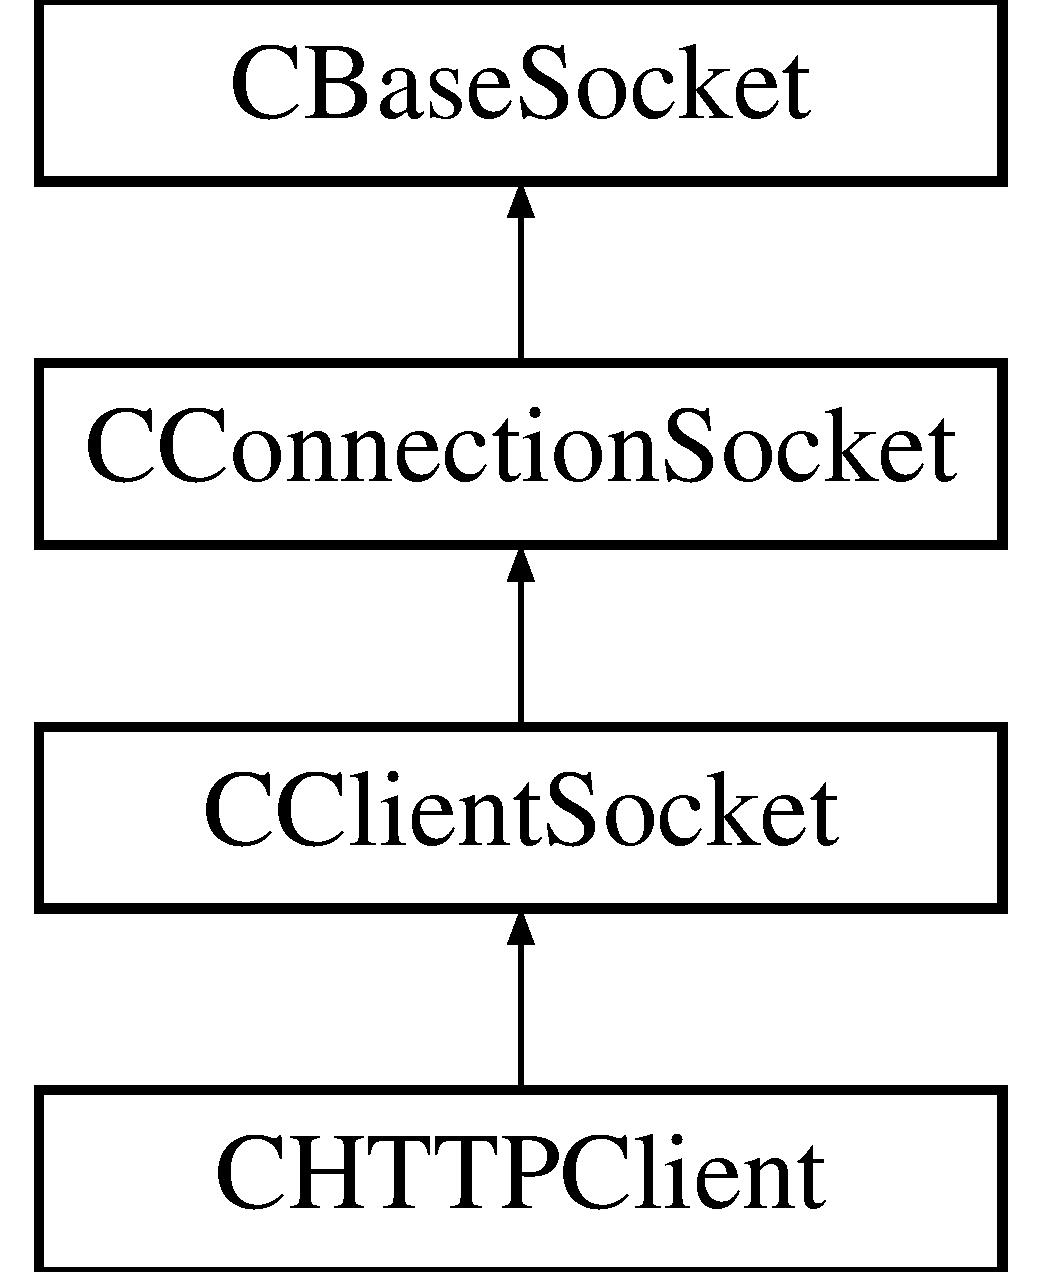
\includegraphics[height=4.000000cm]{class_c_h_t_t_p_client}
\end{center}
\end{figure}
\subsection*{\-Public \-Member \-Functions}
\begin{DoxyCompactItemize}
\item 
\hyperlink{class_c_h_t_t_p_client_a57b036ec3060bc82ae39b6be5322c532}{\-C\-H\-T\-T\-P\-Client} ()
\item 
virtual \hyperlink{class_c_h_t_t_p_client_a3bdb68b5ce1e9c532b2acba2b096eae8}{$\sim$\-C\-H\-T\-T\-P\-Client} ()
\item 
\hyperlink{_cpclient_8h_a3be13892ae7076009afcf121347dd319}{\-B\-O\-O\-L} \hyperlink{class_c_h_t_t_p_client_a3a63aeec6ef9c56a2d8c60641d1cfe7b}{\-Check\-Connect} (const char $\ast$sz\-Host, \hyperlink{_cpclient_8h_a3be13892ae7076009afcf121347dd319}{\-B\-O\-O\-L} b\-Secure, long l\-Port, const char $\ast$sz\-Proxy, long l\-Proxy\-Port, const char $\ast$sz\-Proxy\-User, const char $\ast$sz\-Proxy\-Pswd, long dw\-Timeout)
\begin{DoxyCompactList}\small\item\em \-Connect, even through a proxy. \end{DoxyCompactList}\item 
\hyperlink{_cpclient_8h_a3be13892ae7076009afcf121347dd319}{\-B\-O\-O\-L} \hyperlink{class_c_h_t_t_p_client_a30c615b243b825ada901e671aa1ac420}{\-Get\-H\-T\-T\-P\-Bytes\-Received} (long \&dw\-Length)
\item 
\hyperlink{_cpclient_8h_a3be13892ae7076009afcf121347dd319}{\-B\-O\-O\-L} \hyperlink{class_c_h_t_t_p_client_a088f8e9749c7f4912c2e3de05573069b}{\-Get\-H\-T\-T\-P\-Content} (char $\ast$lp\-Buffer)
\item 
\hyperlink{_cpclient_8h_a3be13892ae7076009afcf121347dd319}{\-B\-O\-O\-L} \hyperlink{class_c_h_t_t_p_client_a831e33c4c95d4e2b02acb299e4c9933f}{\-Get\-H\-T\-T\-P\-Content\-Type} (char $\ast$lp\-Buffer)
\item 
\hyperlink{_cpclient_8h_a3be13892ae7076009afcf121347dd319}{\-B\-O\-O\-L} \hyperlink{class_c_h_t_t_p_client_ab4b0c28fe04c67c29ee3facbad06c764}{\-Get\-H\-T\-T\-P\-Last\-Modified} (char $\ast$lp\-Buffer)
\item 
\hyperlink{_cpclient_8h_a3be13892ae7076009afcf121347dd319}{\-B\-O\-O\-L} \hyperlink{class_c_h_t_t_p_client_ad832d1fd8d84430248279deb2bff4659}{\-Get\-H\-T\-T\-P\-New\-Location} (char $\ast$lp\-Buffer)
\item 
\hyperlink{_cpclient_8h_a3be13892ae7076009afcf121347dd319}{\-B\-O\-O\-L} \hyperlink{class_c_h_t_t_p_client_a3af2141e7152ee9db4a8833b96676af4}{\-Get\-H\-T\-T\-P\-Server} (char $\ast$lp\-Buffer)
\item 
\hyperlink{_cpclient_8h_a3be13892ae7076009afcf121347dd319}{\-B\-O\-O\-L} \hyperlink{class_c_h_t_t_p_client_a7562d00f8b4ab28fb1a457c3898c96b0}{\-Get\-H\-T\-T\-P\-Status} (long \&dw\-Status)
\item 
\hyperlink{_cpclient_8h_a3be13892ae7076009afcf121347dd319}{\-B\-O\-O\-L} \hyperlink{class_c_h_t_t_p_client_ac7c48dc326c9f3760d6edf34de812257}{\-Send\-Request} (const char $\ast$sz\-Host, const char $\ast$sz\-Host\-Name, const char $\ast$sz\-Path, const char $\ast$sz\-User\-I\-D, const char $\ast$sz\-Password, long l\-Port, const char $\ast$sz\-Proxy, long l\-Proxy\-Port, const char $\ast$sz\-Proxy\-User, const char $\ast$sz\-Proxy\-Pswd, const char $\ast$sz\-User\-Agent, const char $\ast$sz\-Post, long dw\-Time\-Out, const char $\ast$sz\-Transaction=\-N\-U\-L\-L)
\begin{DoxyCompactList}\small\item\em \-Send a request. \end{DoxyCompactList}\end{DoxyCompactItemize}
\subsection*{\-Public \-Attributes}
\begin{DoxyCompactItemize}
\item 
\hyperlink{_cpclient_8h_a3be13892ae7076009afcf121347dd319}{\-B\-O\-O\-L} \hyperlink{class_c_h_t_t_p_client_a9bb4f347e03b75be4adc9efe04ec1284}{b\-Read\-Complete}
\item 
\hyperlink{_cpclient_8h_a3be13892ae7076009afcf121347dd319}{\-B\-O\-O\-L} \hyperlink{class_c_h_t_t_p_client_a59e05bc90f7b71663e3b87c06c55721e}{b\-Connect\-Failed}
\item 
long \hyperlink{class_c_h_t_t_p_client_abaa4f1ce357ce53d5087281ad27c9c1b}{dw\-Start\-Time}
\item 
long \hyperlink{class_c_h_t_t_p_client_a88849e78a493edc3c349f3ada5ee86c2}{dw\-First\-Byte}
\item 
long \hyperlink{class_c_h_t_t_p_client_a7461aa9373197650c49ab680e6536d22}{dw\-Last\-Byte}
\item 
string \hyperlink{class_c_h_t_t_p_client_ae0232e77c7c396d7a6708139f6379ef7}{s\-Debug\-Send\-Header}
\item 
string \hyperlink{class_c_h_t_t_p_client_ad89f9c067334f868606ba6d00f3afdab}{s\-Debug\-Recv\-Header}
\end{DoxyCompactItemize}
\subsection*{\-Protected \-Member \-Functions}
\begin{DoxyCompactItemize}
\item 
\hyperlink{_cpclient_8h_a6464f7480a0fd0ee170cba12b2c0497f}{void} \hyperlink{class_c_h_t_t_p_client_a46b8b55050d3ca135be8f11c55c5caf4}{\-Delete\-Cookie\-File} (const char $\ast$lp\-Name)
\item 
\hyperlink{_cpclient_8h_a6464f7480a0fd0ee170cba12b2c0497f}{void} \hyperlink{class_c_h_t_t_p_client_ac55d4579d952c8e9956dc437829cab00}{\-Disconnected} ()
\begin{DoxyCompactList}\small\item\em \-When the \-Service\-Connection\-Thread stops, this gets called. \end{DoxyCompactList}\item 
long \hyperlink{class_c_h_t_t_p_client_aec2f07936dd875e474abf6328414277a}{\-Get\-Time\-Left} (long dw\-Timeout, long dw\-Start)
\item 
\hyperlink{_cpclient_8h_a3be13892ae7076009afcf121347dd319}{\-B\-O\-O\-L} \hyperlink{class_c_h_t_t_p_client_affd3e6e5d6e03d95811dc869b49a00d1}{\-Read\-Cookie\-File} (const char $\ast$lp\-Name)
\item 
\hyperlink{_cpclient_8h_a6464f7480a0fd0ee170cba12b2c0497f}{void} \hyperlink{class_c_h_t_t_p_client_aa29af77553bea44f03920289e2123276}{\-Parse\-Header} ()
\item 
\hyperlink{_cpclient_8h_a3be13892ae7076009afcf121347dd319}{\-B\-O\-O\-L} \hyperlink{class_c_h_t_t_p_client_aaed7b63de2d4e3418366356809fba360}{\-Process\-Data} (unsigned char $\ast$lp\-Data, int i\-Len)
\begin{DoxyCompactList}\small\item\em \-Pure virtual function to process data. \end{DoxyCompactList}\item 
\hyperlink{_cpclient_8h_a6464f7480a0fd0ee170cba12b2c0497f}{void} \hyperlink{class_c_h_t_t_p_client_a348753a2e7fb2c93ae63d64c8da7111c}{\-Request\-Complete} ()
\item 
\hyperlink{_cpclient_8h_a6464f7480a0fd0ee170cba12b2c0497f}{void} \hyperlink{class_c_h_t_t_p_client_aa69904a0714165742a791446e776cfcb}{\-Send\-Cookie} (char $\ast$lp\-Buffer)
\item 
\hyperlink{_cpclient_8h_a3be13892ae7076009afcf121347dd319}{\-B\-O\-O\-L} \hyperlink{class_c_h_t_t_p_client_ac18c2a841c3645a01acfdc3e512c7a7e}{\-Write\-Cookie\-File} (const char $\ast$lp\-Name)
\end{DoxyCompactItemize}
\subsection*{\-Protected \-Attributes}
\begin{DoxyCompactItemize}
\item 
\hyperlink{_cpclient_8h_a3be13892ae7076009afcf121347dd319}{\-B\-O\-O\-L} \hyperlink{class_c_h_t_t_p_client_aa2db4dc9f1177eef59e79ff1970a4a06}{b\-Header}
\item 
\hyperlink{_cpclient_8h_a3be13892ae7076009afcf121347dd319}{\-B\-O\-O\-L} \hyperlink{class_c_h_t_t_p_client_a98a9f41337106c89ca4331d3ee067735}{b\-Head\-Request}
\item 
\hyperlink{class_c_x_plat_event}{\-C\-X\-Plat\-Event} \hyperlink{class_c_h_t_t_p_client_a1ac75d26c210602da43085a9ba1de5bb}{c\-Recv\-Event}
\item 
string \hyperlink{class_c_h_t_t_p_client_ab8d840e3a99e3092df067a218c25e621}{c\-Header}
\item 
string \hyperlink{class_c_h_t_t_p_client_a71cb458d2508e65189f0c65dba6d465d}{c\-Header\-Lwr}
\item 
string \hyperlink{class_c_h_t_t_p_client_a7c814dc76e1feb17be827cfa58246f5e}{c\-Content}
\item 
string \hyperlink{class_c_h_t_t_p_client_a2c8833f6431a9449a2ca776d3b75fdb9}{c\-Content\-Type}
\item 
string \hyperlink{class_c_h_t_t_p_client_a9913b3d73cb9a8172a8ca5e13d39088f}{c\-Last\-Modified}
\item 
string \hyperlink{class_c_h_t_t_p_client_a2d2289bf6605dbe853143fb523f81058}{c\-Location}
\item 
string \hyperlink{class_c_h_t_t_p_client_acbcb5dd8619fbba37910ca522a0bc1a4}{c\-Server}
\item 
string \hyperlink{class_c_h_t_t_p_client_ab9788ca9dcc416a443622abb3ce44b70}{c\-Domain}
\item 
string \hyperlink{class_c_h_t_t_p_client_a7f2cc6944a2535539772f62b51f0c568}{c\-Path}
\item 
string \hyperlink{class_c_h_t_t_p_client_aead239b82d8415a05884cafebf5a384a}{c\-Cookie\-Buf}
\item 
string \hyperlink{class_c_h_t_t_p_client_adbc5e3e3b321c3179b986f2ed2ff0eb1}{c\-Transaction}
\item 
string \hyperlink{class_c_h_t_t_p_client_aa4092d7fea50e76e30f3269479253db6}{c\-Request\-Num}
\item 
long \hyperlink{class_c_h_t_t_p_client_a3840ab9a7468b62900613238c47c36cb}{l\-Content\-Length}
\item 
long \hyperlink{class_c_h_t_t_p_client_a3912e2379d3a00b9a0e671abab1dd0b7}{l\-Received\-Length}
\item 
char \hyperlink{class_c_h_t_t_p_client_aff047143e60597632e37899b10fab8e2}{sz\-Send\-Buffer} \mbox{[}\hyperlink{rtminet_8h_aff8960325dbc7b5bf858b614b502da19}{\-I\-N\-T\-E\-R\-N\-E\-T\-\_\-\-M\-A\-X\-\_\-\-U\-R\-L\-\_\-\-L\-E\-N\-G\-T\-H\-\_\-\-R\-T\-M}+1\mbox{]}
\item 
char \hyperlink{class_c_h_t_t_p_client_a05468a0fa4fd07830d9dc0fd0fba55ee}{sz\-Status} \mbox{[}4\mbox{]}
\end{DoxyCompactItemize}


\subsection{\-Detailed \-Description}
\hyperlink{class_c_h_t_t_p_client}{\-C\-H\-T\-T\-P\-Client} -\/ make a connection and fetch a \-U\-R\-L. 

\-Definition at line 41 of file \-C\-H\-T\-T\-P\-Client.\-h.



\subsection{\-Constructor \& \-Destructor \-Documentation}
\hypertarget{class_c_h_t_t_p_client_a57b036ec3060bc82ae39b6be5322c532}{\index{\-C\-H\-T\-T\-P\-Client@{\-C\-H\-T\-T\-P\-Client}!\-C\-H\-T\-T\-P\-Client@{\-C\-H\-T\-T\-P\-Client}}
\index{\-C\-H\-T\-T\-P\-Client@{\-C\-H\-T\-T\-P\-Client}!CHTTPClient@{\-C\-H\-T\-T\-P\-Client}}
\subsubsection[{\-C\-H\-T\-T\-P\-Client}]{\setlength{\rightskip}{0pt plus 5cm}{\bf \-C\-H\-T\-T\-P\-Client\-::\-C\-H\-T\-T\-P\-Client} (
\begin{DoxyParamCaption}
{}
\end{DoxyParamCaption}
)}}\label{class_c_h_t_t_p_client_a57b036ec3060bc82ae39b6be5322c532}


\-Definition at line 55 of file \-C\-H\-T\-T\-P\-Client.\-cpp.

\hypertarget{class_c_h_t_t_p_client_a3bdb68b5ce1e9c532b2acba2b096eae8}{\index{\-C\-H\-T\-T\-P\-Client@{\-C\-H\-T\-T\-P\-Client}!$\sim$\-C\-H\-T\-T\-P\-Client@{$\sim$\-C\-H\-T\-T\-P\-Client}}
\index{$\sim$\-C\-H\-T\-T\-P\-Client@{$\sim$\-C\-H\-T\-T\-P\-Client}!CHTTPClient@{\-C\-H\-T\-T\-P\-Client}}
\subsubsection[{$\sim$\-C\-H\-T\-T\-P\-Client}]{\setlength{\rightskip}{0pt plus 5cm}{\bf \-C\-H\-T\-T\-P\-Client\-::$\sim$\-C\-H\-T\-T\-P\-Client} (
\begin{DoxyParamCaption}
{}
\end{DoxyParamCaption}
)\hspace{0.3cm}{\ttfamily  \mbox{[}virtual\mbox{]}}}}\label{class_c_h_t_t_p_client_a3bdb68b5ce1e9c532b2acba2b096eae8}


\-Definition at line 63 of file \-C\-H\-T\-T\-P\-Client.\-cpp.



\subsection{\-Member \-Function \-Documentation}
\hypertarget{class_c_h_t_t_p_client_a3a63aeec6ef9c56a2d8c60641d1cfe7b}{\index{\-C\-H\-T\-T\-P\-Client@{\-C\-H\-T\-T\-P\-Client}!\-Check\-Connect@{\-Check\-Connect}}
\index{\-Check\-Connect@{\-Check\-Connect}!CHTTPClient@{\-C\-H\-T\-T\-P\-Client}}
\subsubsection[{\-Check\-Connect}]{\setlength{\rightskip}{0pt plus 5cm}{\bf \-B\-O\-O\-L} {\bf \-C\-H\-T\-T\-P\-Client\-::\-Check\-Connect} (
\begin{DoxyParamCaption}
\item[{const char $\ast$}]{sz\-Host, }
\item[{{\bf \-B\-O\-O\-L}}]{b\-Secure, }
\item[{long}]{l\-Port, }
\item[{const char $\ast$}]{sz\-Proxy, }
\item[{long}]{l\-Proxy\-Port, }
\item[{const char $\ast$}]{sz\-Proxy\-User, }
\item[{const char $\ast$}]{sz\-Proxy\-Pswd, }
\item[{long}]{dw\-Timeout}
\end{DoxyParamCaption}
)}}\label{class_c_h_t_t_p_client_a3a63aeec6ef9c56a2d8c60641d1cfe7b}


\-Connect, even through a proxy. 



\-Definition at line 1175 of file \-C\-H\-T\-T\-P\-Client.\-cpp.

\hypertarget{class_c_h_t_t_p_client_a46b8b55050d3ca135be8f11c55c5caf4}{\index{\-C\-H\-T\-T\-P\-Client@{\-C\-H\-T\-T\-P\-Client}!\-Delete\-Cookie\-File@{\-Delete\-Cookie\-File}}
\index{\-Delete\-Cookie\-File@{\-Delete\-Cookie\-File}!CHTTPClient@{\-C\-H\-T\-T\-P\-Client}}
\subsubsection[{\-Delete\-Cookie\-File}]{\setlength{\rightskip}{0pt plus 5cm}{\bf void} {\bf \-C\-H\-T\-T\-P\-Client\-::\-Delete\-Cookie\-File} (
\begin{DoxyParamCaption}
\item[{const char $\ast$}]{lp\-Name}
\end{DoxyParamCaption}
)\hspace{0.3cm}{\ttfamily  \mbox{[}protected\mbox{]}}}}\label{class_c_h_t_t_p_client_a46b8b55050d3ca135be8f11c55c5caf4}


\-Definition at line 1069 of file \-C\-H\-T\-T\-P\-Client.\-cpp.

\hypertarget{class_c_h_t_t_p_client_ac55d4579d952c8e9956dc437829cab00}{\index{\-C\-H\-T\-T\-P\-Client@{\-C\-H\-T\-T\-P\-Client}!\-Disconnected@{\-Disconnected}}
\index{\-Disconnected@{\-Disconnected}!CHTTPClient@{\-C\-H\-T\-T\-P\-Client}}
\subsubsection[{\-Disconnected}]{\setlength{\rightskip}{0pt plus 5cm}{\bf void} {\bf \-C\-H\-T\-T\-P\-Client\-::\-Disconnected} (
\begin{DoxyParamCaption}
{}
\end{DoxyParamCaption}
)\hspace{0.3cm}{\ttfamily  \mbox{[}protected, virtual\mbox{]}}}}\label{class_c_h_t_t_p_client_ac55d4579d952c8e9956dc437829cab00}


\-When the \-Service\-Connection\-Thread stops, this gets called. 

\-Called when the socket is disconnecting \-W\-A\-R\-N\-I\-N\-G\-: this may occasionally get called more than once -\/ code appropriately 

\-Reimplemented from \hyperlink{class_c_connection_socket_a2d991ece47fd9c86366af981c70d51fc}{\-C\-Connection\-Socket}.



\-Definition at line 196 of file \-C\-H\-T\-T\-P\-Client.\-cpp.

\hypertarget{class_c_h_t_t_p_client_a30c615b243b825ada901e671aa1ac420}{\index{\-C\-H\-T\-T\-P\-Client@{\-C\-H\-T\-T\-P\-Client}!\-Get\-H\-T\-T\-P\-Bytes\-Received@{\-Get\-H\-T\-T\-P\-Bytes\-Received}}
\index{\-Get\-H\-T\-T\-P\-Bytes\-Received@{\-Get\-H\-T\-T\-P\-Bytes\-Received}!CHTTPClient@{\-C\-H\-T\-T\-P\-Client}}
\subsubsection[{\-Get\-H\-T\-T\-P\-Bytes\-Received}]{\setlength{\rightskip}{0pt plus 5cm}{\bf \-B\-O\-O\-L} {\bf \-C\-H\-T\-T\-P\-Client\-::\-Get\-H\-T\-T\-P\-Bytes\-Received} (
\begin{DoxyParamCaption}
\item[{long \&}]{dw\-Length}
\end{DoxyParamCaption}
)}}\label{class_c_h_t_t_p_client_a30c615b243b825ada901e671aa1ac420}


\-Definition at line 1103 of file \-C\-H\-T\-T\-P\-Client.\-cpp.

\hypertarget{class_c_h_t_t_p_client_a088f8e9749c7f4912c2e3de05573069b}{\index{\-C\-H\-T\-T\-P\-Client@{\-C\-H\-T\-T\-P\-Client}!\-Get\-H\-T\-T\-P\-Content@{\-Get\-H\-T\-T\-P\-Content}}
\index{\-Get\-H\-T\-T\-P\-Content@{\-Get\-H\-T\-T\-P\-Content}!CHTTPClient@{\-C\-H\-T\-T\-P\-Client}}
\subsubsection[{\-Get\-H\-T\-T\-P\-Content}]{\setlength{\rightskip}{0pt plus 5cm}{\bf \-B\-O\-O\-L} {\bf \-C\-H\-T\-T\-P\-Client\-::\-Get\-H\-T\-T\-P\-Content} (
\begin{DoxyParamCaption}
\item[{char $\ast$}]{lp\-Buffer}
\end{DoxyParamCaption}
)}}\label{class_c_h_t_t_p_client_a088f8e9749c7f4912c2e3de05573069b}


\-Definition at line 1112 of file \-C\-H\-T\-T\-P\-Client.\-cpp.

\hypertarget{class_c_h_t_t_p_client_a831e33c4c95d4e2b02acb299e4c9933f}{\index{\-C\-H\-T\-T\-P\-Client@{\-C\-H\-T\-T\-P\-Client}!\-Get\-H\-T\-T\-P\-Content\-Type@{\-Get\-H\-T\-T\-P\-Content\-Type}}
\index{\-Get\-H\-T\-T\-P\-Content\-Type@{\-Get\-H\-T\-T\-P\-Content\-Type}!CHTTPClient@{\-C\-H\-T\-T\-P\-Client}}
\subsubsection[{\-Get\-H\-T\-T\-P\-Content\-Type}]{\setlength{\rightskip}{0pt plus 5cm}{\bf \-B\-O\-O\-L} {\bf \-C\-H\-T\-T\-P\-Client\-::\-Get\-H\-T\-T\-P\-Content\-Type} (
\begin{DoxyParamCaption}
\item[{char $\ast$}]{lp\-Buffer}
\end{DoxyParamCaption}
)}}\label{class_c_h_t_t_p_client_a831e33c4c95d4e2b02acb299e4c9933f}


\-Definition at line 1121 of file \-C\-H\-T\-T\-P\-Client.\-cpp.

\hypertarget{class_c_h_t_t_p_client_ab4b0c28fe04c67c29ee3facbad06c764}{\index{\-C\-H\-T\-T\-P\-Client@{\-C\-H\-T\-T\-P\-Client}!\-Get\-H\-T\-T\-P\-Last\-Modified@{\-Get\-H\-T\-T\-P\-Last\-Modified}}
\index{\-Get\-H\-T\-T\-P\-Last\-Modified@{\-Get\-H\-T\-T\-P\-Last\-Modified}!CHTTPClient@{\-C\-H\-T\-T\-P\-Client}}
\subsubsection[{\-Get\-H\-T\-T\-P\-Last\-Modified}]{\setlength{\rightskip}{0pt plus 5cm}{\bf \-B\-O\-O\-L} {\bf \-C\-H\-T\-T\-P\-Client\-::\-Get\-H\-T\-T\-P\-Last\-Modified} (
\begin{DoxyParamCaption}
\item[{char $\ast$}]{lp\-Buffer}
\end{DoxyParamCaption}
)}}\label{class_c_h_t_t_p_client_ab4b0c28fe04c67c29ee3facbad06c764}


\-Definition at line 1130 of file \-C\-H\-T\-T\-P\-Client.\-cpp.

\hypertarget{class_c_h_t_t_p_client_ad832d1fd8d84430248279deb2bff4659}{\index{\-C\-H\-T\-T\-P\-Client@{\-C\-H\-T\-T\-P\-Client}!\-Get\-H\-T\-T\-P\-New\-Location@{\-Get\-H\-T\-T\-P\-New\-Location}}
\index{\-Get\-H\-T\-T\-P\-New\-Location@{\-Get\-H\-T\-T\-P\-New\-Location}!CHTTPClient@{\-C\-H\-T\-T\-P\-Client}}
\subsubsection[{\-Get\-H\-T\-T\-P\-New\-Location}]{\setlength{\rightskip}{0pt plus 5cm}{\bf \-B\-O\-O\-L} {\bf \-C\-H\-T\-T\-P\-Client\-::\-Get\-H\-T\-T\-P\-New\-Location} (
\begin{DoxyParamCaption}
\item[{char $\ast$}]{lp\-Buffer}
\end{DoxyParamCaption}
)}}\label{class_c_h_t_t_p_client_ad832d1fd8d84430248279deb2bff4659}


\-Definition at line 1139 of file \-C\-H\-T\-T\-P\-Client.\-cpp.

\hypertarget{class_c_h_t_t_p_client_a3af2141e7152ee9db4a8833b96676af4}{\index{\-C\-H\-T\-T\-P\-Client@{\-C\-H\-T\-T\-P\-Client}!\-Get\-H\-T\-T\-P\-Server@{\-Get\-H\-T\-T\-P\-Server}}
\index{\-Get\-H\-T\-T\-P\-Server@{\-Get\-H\-T\-T\-P\-Server}!CHTTPClient@{\-C\-H\-T\-T\-P\-Client}}
\subsubsection[{\-Get\-H\-T\-T\-P\-Server}]{\setlength{\rightskip}{0pt plus 5cm}{\bf \-B\-O\-O\-L} {\bf \-C\-H\-T\-T\-P\-Client\-::\-Get\-H\-T\-T\-P\-Server} (
\begin{DoxyParamCaption}
\item[{char $\ast$}]{lp\-Buffer}
\end{DoxyParamCaption}
)}}\label{class_c_h_t_t_p_client_a3af2141e7152ee9db4a8833b96676af4}


\-Definition at line 1148 of file \-C\-H\-T\-T\-P\-Client.\-cpp.

\hypertarget{class_c_h_t_t_p_client_a7562d00f8b4ab28fb1a457c3898c96b0}{\index{\-C\-H\-T\-T\-P\-Client@{\-C\-H\-T\-T\-P\-Client}!\-Get\-H\-T\-T\-P\-Status@{\-Get\-H\-T\-T\-P\-Status}}
\index{\-Get\-H\-T\-T\-P\-Status@{\-Get\-H\-T\-T\-P\-Status}!CHTTPClient@{\-C\-H\-T\-T\-P\-Client}}
\subsubsection[{\-Get\-H\-T\-T\-P\-Status}]{\setlength{\rightskip}{0pt plus 5cm}{\bf \-B\-O\-O\-L} {\bf \-C\-H\-T\-T\-P\-Client\-::\-Get\-H\-T\-T\-P\-Status} (
\begin{DoxyParamCaption}
\item[{long \&}]{dw\-Status}
\end{DoxyParamCaption}
)}}\label{class_c_h_t_t_p_client_a7562d00f8b4ab28fb1a457c3898c96b0}


\-Definition at line 1085 of file \-C\-H\-T\-T\-P\-Client.\-cpp.

\hypertarget{class_c_h_t_t_p_client_aec2f07936dd875e474abf6328414277a}{\index{\-C\-H\-T\-T\-P\-Client@{\-C\-H\-T\-T\-P\-Client}!\-Get\-Time\-Left@{\-Get\-Time\-Left}}
\index{\-Get\-Time\-Left@{\-Get\-Time\-Left}!CHTTPClient@{\-C\-H\-T\-T\-P\-Client}}
\subsubsection[{\-Get\-Time\-Left}]{\setlength{\rightskip}{0pt plus 5cm}long {\bf \-C\-H\-T\-T\-P\-Client\-::\-Get\-Time\-Left} (
\begin{DoxyParamCaption}
\item[{long}]{dw\-Timeout, }
\item[{long}]{dw\-Start}
\end{DoxyParamCaption}
)\hspace{0.3cm}{\ttfamily  \mbox{[}protected\mbox{]}}}}\label{class_c_h_t_t_p_client_aec2f07936dd875e474abf6328414277a}


\-Definition at line 1160 of file \-C\-H\-T\-T\-P\-Client.\-cpp.

\hypertarget{class_c_h_t_t_p_client_aa29af77553bea44f03920289e2123276}{\index{\-C\-H\-T\-T\-P\-Client@{\-C\-H\-T\-T\-P\-Client}!\-Parse\-Header@{\-Parse\-Header}}
\index{\-Parse\-Header@{\-Parse\-Header}!CHTTPClient@{\-C\-H\-T\-T\-P\-Client}}
\subsubsection[{\-Parse\-Header}]{\setlength{\rightskip}{0pt plus 5cm}{\bf void} {\bf \-C\-H\-T\-T\-P\-Client\-::\-Parse\-Header} (
\begin{DoxyParamCaption}
{}
\end{DoxyParamCaption}
)\hspace{0.3cm}{\ttfamily  \mbox{[}protected\mbox{]}}}}\label{class_c_h_t_t_p_client_aa29af77553bea44f03920289e2123276}


\-Definition at line 741 of file \-C\-H\-T\-T\-P\-Client.\-cpp.

\hypertarget{class_c_h_t_t_p_client_aaed7b63de2d4e3418366356809fba360}{\index{\-C\-H\-T\-T\-P\-Client@{\-C\-H\-T\-T\-P\-Client}!\-Process\-Data@{\-Process\-Data}}
\index{\-Process\-Data@{\-Process\-Data}!CHTTPClient@{\-C\-H\-T\-T\-P\-Client}}
\subsubsection[{\-Process\-Data}]{\setlength{\rightskip}{0pt plus 5cm}{\bf \-B\-O\-O\-L} {\bf \-C\-H\-T\-T\-P\-Client\-::\-Process\-Data} (
\begin{DoxyParamCaption}
\item[{unsigned char $\ast$}]{lp\-Data, }
\item[{int}]{i\-Len}
\end{DoxyParamCaption}
)\hspace{0.3cm}{\ttfamily  \mbox{[}protected, virtual\mbox{]}}}}\label{class_c_h_t_t_p_client_aaed7b63de2d4e3418366356809fba360}


\-Pure virtual function to process data. 



\-Implements \hyperlink{class_c_connection_socket_a11c2aef1e11bbac03c72ec9444b8e85f}{\-C\-Connection\-Socket}.



\-Definition at line 93 of file \-C\-H\-T\-T\-P\-Client.\-cpp.

\hypertarget{class_c_h_t_t_p_client_affd3e6e5d6e03d95811dc869b49a00d1}{\index{\-C\-H\-T\-T\-P\-Client@{\-C\-H\-T\-T\-P\-Client}!\-Read\-Cookie\-File@{\-Read\-Cookie\-File}}
\index{\-Read\-Cookie\-File@{\-Read\-Cookie\-File}!CHTTPClient@{\-C\-H\-T\-T\-P\-Client}}
\subsubsection[{\-Read\-Cookie\-File}]{\setlength{\rightskip}{0pt plus 5cm}{\bf \-B\-O\-O\-L} {\bf \-C\-H\-T\-T\-P\-Client\-::\-Read\-Cookie\-File} (
\begin{DoxyParamCaption}
\item[{const char $\ast$}]{lp\-Name}
\end{DoxyParamCaption}
)\hspace{0.3cm}{\ttfamily  \mbox{[}protected\mbox{]}}}}\label{class_c_h_t_t_p_client_affd3e6e5d6e03d95811dc869b49a00d1}


\-Definition at line 987 of file \-C\-H\-T\-T\-P\-Client.\-cpp.

\hypertarget{class_c_h_t_t_p_client_a348753a2e7fb2c93ae63d64c8da7111c}{\index{\-C\-H\-T\-T\-P\-Client@{\-C\-H\-T\-T\-P\-Client}!\-Request\-Complete@{\-Request\-Complete}}
\index{\-Request\-Complete@{\-Request\-Complete}!CHTTPClient@{\-C\-H\-T\-T\-P\-Client}}
\subsubsection[{\-Request\-Complete}]{\setlength{\rightskip}{0pt plus 5cm}{\bf void} {\bf \-C\-H\-T\-T\-P\-Client\-::\-Request\-Complete} (
\begin{DoxyParamCaption}
{}
\end{DoxyParamCaption}
)\hspace{0.3cm}{\ttfamily  \mbox{[}protected\mbox{]}}}}\label{class_c_h_t_t_p_client_a348753a2e7fb2c93ae63d64c8da7111c}


\-Definition at line 181 of file \-C\-H\-T\-T\-P\-Client.\-cpp.

\hypertarget{class_c_h_t_t_p_client_aa69904a0714165742a791446e776cfcb}{\index{\-C\-H\-T\-T\-P\-Client@{\-C\-H\-T\-T\-P\-Client}!\-Send\-Cookie@{\-Send\-Cookie}}
\index{\-Send\-Cookie@{\-Send\-Cookie}!CHTTPClient@{\-C\-H\-T\-T\-P\-Client}}
\subsubsection[{\-Send\-Cookie}]{\setlength{\rightskip}{0pt plus 5cm}{\bf void} {\bf \-C\-H\-T\-T\-P\-Client\-::\-Send\-Cookie} (
\begin{DoxyParamCaption}
\item[{char $\ast$}]{lp\-Buffer}
\end{DoxyParamCaption}
)\hspace{0.3cm}{\ttfamily  \mbox{[}protected\mbox{]}}}}\label{class_c_h_t_t_p_client_aa69904a0714165742a791446e776cfcb}


\-Definition at line 916 of file \-C\-H\-T\-T\-P\-Client.\-cpp.

\hypertarget{class_c_h_t_t_p_client_ac7c48dc326c9f3760d6edf34de812257}{\index{\-C\-H\-T\-T\-P\-Client@{\-C\-H\-T\-T\-P\-Client}!\-Send\-Request@{\-Send\-Request}}
\index{\-Send\-Request@{\-Send\-Request}!CHTTPClient@{\-C\-H\-T\-T\-P\-Client}}
\subsubsection[{\-Send\-Request}]{\setlength{\rightskip}{0pt plus 5cm}{\bf \-B\-O\-O\-L} {\bf \-C\-H\-T\-T\-P\-Client\-::\-Send\-Request} (
\begin{DoxyParamCaption}
\item[{const char $\ast$}]{sz\-Host, }
\item[{const char $\ast$}]{sz\-Host\-Name, }
\item[{const char $\ast$}]{sz\-Path, }
\item[{const char $\ast$}]{sz\-User\-I\-D, }
\item[{const char $\ast$}]{sz\-Password, }
\item[{long}]{l\-Port, }
\item[{const char $\ast$}]{sz\-Proxy, }
\item[{long}]{l\-Proxy\-Port, }
\item[{const char $\ast$}]{sz\-Proxy\-User, }
\item[{const char $\ast$}]{sz\-Proxy\-Pswd, }
\item[{const char $\ast$}]{sz\-User\-Agent, }
\item[{const char $\ast$}]{sz\-Post, }
\item[{long}]{dw\-Time\-Out, }
\item[{const char $\ast$}]{sz\-Transaction = {\ttfamily \-N\-U\-L\-L}}
\end{DoxyParamCaption}
)}}\label{class_c_h_t_t_p_client_ac7c48dc326c9f3760d6edf34de812257}


\-Send a request. 



\-Definition at line 204 of file \-C\-H\-T\-T\-P\-Client.\-cpp.

\hypertarget{class_c_h_t_t_p_client_ac18c2a841c3645a01acfdc3e512c7a7e}{\index{\-C\-H\-T\-T\-P\-Client@{\-C\-H\-T\-T\-P\-Client}!\-Write\-Cookie\-File@{\-Write\-Cookie\-File}}
\index{\-Write\-Cookie\-File@{\-Write\-Cookie\-File}!CHTTPClient@{\-C\-H\-T\-T\-P\-Client}}
\subsubsection[{\-Write\-Cookie\-File}]{\setlength{\rightskip}{0pt plus 5cm}{\bf \-B\-O\-O\-L} {\bf \-C\-H\-T\-T\-P\-Client\-::\-Write\-Cookie\-File} (
\begin{DoxyParamCaption}
\item[{const char $\ast$}]{lp\-Name}
\end{DoxyParamCaption}
)\hspace{0.3cm}{\ttfamily  \mbox{[}protected\mbox{]}}}}\label{class_c_h_t_t_p_client_ac18c2a841c3645a01acfdc3e512c7a7e}


\-Definition at line 1037 of file \-C\-H\-T\-T\-P\-Client.\-cpp.



\subsection{\-Member \-Data \-Documentation}
\hypertarget{class_c_h_t_t_p_client_a59e05bc90f7b71663e3b87c06c55721e}{\index{\-C\-H\-T\-T\-P\-Client@{\-C\-H\-T\-T\-P\-Client}!b\-Connect\-Failed@{b\-Connect\-Failed}}
\index{b\-Connect\-Failed@{b\-Connect\-Failed}!CHTTPClient@{\-C\-H\-T\-T\-P\-Client}}
\subsubsection[{b\-Connect\-Failed}]{\setlength{\rightskip}{0pt plus 5cm}{\bf \-B\-O\-O\-L} {\bf \-C\-H\-T\-T\-P\-Client\-::b\-Connect\-Failed}}}\label{class_c_h_t_t_p_client_a59e05bc90f7b71663e3b87c06c55721e}


\-Definition at line 104 of file \-C\-H\-T\-T\-P\-Client.\-h.

\hypertarget{class_c_h_t_t_p_client_aa2db4dc9f1177eef59e79ff1970a4a06}{\index{\-C\-H\-T\-T\-P\-Client@{\-C\-H\-T\-T\-P\-Client}!b\-Header@{b\-Header}}
\index{b\-Header@{b\-Header}!CHTTPClient@{\-C\-H\-T\-T\-P\-Client}}
\subsubsection[{b\-Header}]{\setlength{\rightskip}{0pt plus 5cm}{\bf \-B\-O\-O\-L} {\bf \-C\-H\-T\-T\-P\-Client\-::b\-Header}\hspace{0.3cm}{\ttfamily  \mbox{[}protected\mbox{]}}}}\label{class_c_h_t_t_p_client_aa2db4dc9f1177eef59e79ff1970a4a06}


\-Definition at line 130 of file \-C\-H\-T\-T\-P\-Client.\-h.

\hypertarget{class_c_h_t_t_p_client_a98a9f41337106c89ca4331d3ee067735}{\index{\-C\-H\-T\-T\-P\-Client@{\-C\-H\-T\-T\-P\-Client}!b\-Head\-Request@{b\-Head\-Request}}
\index{b\-Head\-Request@{b\-Head\-Request}!CHTTPClient@{\-C\-H\-T\-T\-P\-Client}}
\subsubsection[{b\-Head\-Request}]{\setlength{\rightskip}{0pt plus 5cm}{\bf \-B\-O\-O\-L} {\bf \-C\-H\-T\-T\-P\-Client\-::b\-Head\-Request}\hspace{0.3cm}{\ttfamily  \mbox{[}protected\mbox{]}}}}\label{class_c_h_t_t_p_client_a98a9f41337106c89ca4331d3ee067735}


\-Definition at line 131 of file \-C\-H\-T\-T\-P\-Client.\-h.

\hypertarget{class_c_h_t_t_p_client_a9bb4f347e03b75be4adc9efe04ec1284}{\index{\-C\-H\-T\-T\-P\-Client@{\-C\-H\-T\-T\-P\-Client}!b\-Read\-Complete@{b\-Read\-Complete}}
\index{b\-Read\-Complete@{b\-Read\-Complete}!CHTTPClient@{\-C\-H\-T\-T\-P\-Client}}
\subsubsection[{b\-Read\-Complete}]{\setlength{\rightskip}{0pt plus 5cm}{\bf \-B\-O\-O\-L} {\bf \-C\-H\-T\-T\-P\-Client\-::b\-Read\-Complete}}}\label{class_c_h_t_t_p_client_a9bb4f347e03b75be4adc9efe04ec1284}


\-Definition at line 103 of file \-C\-H\-T\-T\-P\-Client.\-h.

\hypertarget{class_c_h_t_t_p_client_a7c814dc76e1feb17be827cfa58246f5e}{\index{\-C\-H\-T\-T\-P\-Client@{\-C\-H\-T\-T\-P\-Client}!c\-Content@{c\-Content}}
\index{c\-Content@{c\-Content}!CHTTPClient@{\-C\-H\-T\-T\-P\-Client}}
\subsubsection[{c\-Content}]{\setlength{\rightskip}{0pt plus 5cm}string {\bf \-C\-H\-T\-T\-P\-Client\-::c\-Content}\hspace{0.3cm}{\ttfamily  \mbox{[}protected\mbox{]}}}}\label{class_c_h_t_t_p_client_a7c814dc76e1feb17be827cfa58246f5e}


\-Definition at line 135 of file \-C\-H\-T\-T\-P\-Client.\-h.

\hypertarget{class_c_h_t_t_p_client_a2c8833f6431a9449a2ca776d3b75fdb9}{\index{\-C\-H\-T\-T\-P\-Client@{\-C\-H\-T\-T\-P\-Client}!c\-Content\-Type@{c\-Content\-Type}}
\index{c\-Content\-Type@{c\-Content\-Type}!CHTTPClient@{\-C\-H\-T\-T\-P\-Client}}
\subsubsection[{c\-Content\-Type}]{\setlength{\rightskip}{0pt plus 5cm}string {\bf \-C\-H\-T\-T\-P\-Client\-::c\-Content\-Type}\hspace{0.3cm}{\ttfamily  \mbox{[}protected\mbox{]}}}}\label{class_c_h_t_t_p_client_a2c8833f6431a9449a2ca776d3b75fdb9}


\-Definition at line 136 of file \-C\-H\-T\-T\-P\-Client.\-h.

\hypertarget{class_c_h_t_t_p_client_aead239b82d8415a05884cafebf5a384a}{\index{\-C\-H\-T\-T\-P\-Client@{\-C\-H\-T\-T\-P\-Client}!c\-Cookie\-Buf@{c\-Cookie\-Buf}}
\index{c\-Cookie\-Buf@{c\-Cookie\-Buf}!CHTTPClient@{\-C\-H\-T\-T\-P\-Client}}
\subsubsection[{c\-Cookie\-Buf}]{\setlength{\rightskip}{0pt plus 5cm}string {\bf \-C\-H\-T\-T\-P\-Client\-::c\-Cookie\-Buf}\hspace{0.3cm}{\ttfamily  \mbox{[}protected\mbox{]}}}}\label{class_c_h_t_t_p_client_aead239b82d8415a05884cafebf5a384a}


\-Definition at line 142 of file \-C\-H\-T\-T\-P\-Client.\-h.

\hypertarget{class_c_h_t_t_p_client_ab9788ca9dcc416a443622abb3ce44b70}{\index{\-C\-H\-T\-T\-P\-Client@{\-C\-H\-T\-T\-P\-Client}!c\-Domain@{c\-Domain}}
\index{c\-Domain@{c\-Domain}!CHTTPClient@{\-C\-H\-T\-T\-P\-Client}}
\subsubsection[{c\-Domain}]{\setlength{\rightskip}{0pt plus 5cm}string {\bf \-C\-H\-T\-T\-P\-Client\-::c\-Domain}\hspace{0.3cm}{\ttfamily  \mbox{[}protected\mbox{]}}}}\label{class_c_h_t_t_p_client_ab9788ca9dcc416a443622abb3ce44b70}


\-Definition at line 140 of file \-C\-H\-T\-T\-P\-Client.\-h.

\hypertarget{class_c_h_t_t_p_client_ab8d840e3a99e3092df067a218c25e621}{\index{\-C\-H\-T\-T\-P\-Client@{\-C\-H\-T\-T\-P\-Client}!c\-Header@{c\-Header}}
\index{c\-Header@{c\-Header}!CHTTPClient@{\-C\-H\-T\-T\-P\-Client}}
\subsubsection[{c\-Header}]{\setlength{\rightskip}{0pt plus 5cm}string {\bf \-C\-H\-T\-T\-P\-Client\-::c\-Header}\hspace{0.3cm}{\ttfamily  \mbox{[}protected\mbox{]}}}}\label{class_c_h_t_t_p_client_ab8d840e3a99e3092df067a218c25e621}


\-Definition at line 133 of file \-C\-H\-T\-T\-P\-Client.\-h.

\hypertarget{class_c_h_t_t_p_client_a71cb458d2508e65189f0c65dba6d465d}{\index{\-C\-H\-T\-T\-P\-Client@{\-C\-H\-T\-T\-P\-Client}!c\-Header\-Lwr@{c\-Header\-Lwr}}
\index{c\-Header\-Lwr@{c\-Header\-Lwr}!CHTTPClient@{\-C\-H\-T\-T\-P\-Client}}
\subsubsection[{c\-Header\-Lwr}]{\setlength{\rightskip}{0pt plus 5cm}string {\bf \-C\-H\-T\-T\-P\-Client\-::c\-Header\-Lwr}\hspace{0.3cm}{\ttfamily  \mbox{[}protected\mbox{]}}}}\label{class_c_h_t_t_p_client_a71cb458d2508e65189f0c65dba6d465d}


\-Definition at line 134 of file \-C\-H\-T\-T\-P\-Client.\-h.

\hypertarget{class_c_h_t_t_p_client_a9913b3d73cb9a8172a8ca5e13d39088f}{\index{\-C\-H\-T\-T\-P\-Client@{\-C\-H\-T\-T\-P\-Client}!c\-Last\-Modified@{c\-Last\-Modified}}
\index{c\-Last\-Modified@{c\-Last\-Modified}!CHTTPClient@{\-C\-H\-T\-T\-P\-Client}}
\subsubsection[{c\-Last\-Modified}]{\setlength{\rightskip}{0pt plus 5cm}string {\bf \-C\-H\-T\-T\-P\-Client\-::c\-Last\-Modified}\hspace{0.3cm}{\ttfamily  \mbox{[}protected\mbox{]}}}}\label{class_c_h_t_t_p_client_a9913b3d73cb9a8172a8ca5e13d39088f}


\-Definition at line 137 of file \-C\-H\-T\-T\-P\-Client.\-h.

\hypertarget{class_c_h_t_t_p_client_a2d2289bf6605dbe853143fb523f81058}{\index{\-C\-H\-T\-T\-P\-Client@{\-C\-H\-T\-T\-P\-Client}!c\-Location@{c\-Location}}
\index{c\-Location@{c\-Location}!CHTTPClient@{\-C\-H\-T\-T\-P\-Client}}
\subsubsection[{c\-Location}]{\setlength{\rightskip}{0pt plus 5cm}string {\bf \-C\-H\-T\-T\-P\-Client\-::c\-Location}\hspace{0.3cm}{\ttfamily  \mbox{[}protected\mbox{]}}}}\label{class_c_h_t_t_p_client_a2d2289bf6605dbe853143fb523f81058}


\-Definition at line 138 of file \-C\-H\-T\-T\-P\-Client.\-h.

\hypertarget{class_c_h_t_t_p_client_a7f2cc6944a2535539772f62b51f0c568}{\index{\-C\-H\-T\-T\-P\-Client@{\-C\-H\-T\-T\-P\-Client}!c\-Path@{c\-Path}}
\index{c\-Path@{c\-Path}!CHTTPClient@{\-C\-H\-T\-T\-P\-Client}}
\subsubsection[{c\-Path}]{\setlength{\rightskip}{0pt plus 5cm}string {\bf \-C\-H\-T\-T\-P\-Client\-::c\-Path}\hspace{0.3cm}{\ttfamily  \mbox{[}protected\mbox{]}}}}\label{class_c_h_t_t_p_client_a7f2cc6944a2535539772f62b51f0c568}


\-Definition at line 141 of file \-C\-H\-T\-T\-P\-Client.\-h.

\hypertarget{class_c_h_t_t_p_client_a1ac75d26c210602da43085a9ba1de5bb}{\index{\-C\-H\-T\-T\-P\-Client@{\-C\-H\-T\-T\-P\-Client}!c\-Recv\-Event@{c\-Recv\-Event}}
\index{c\-Recv\-Event@{c\-Recv\-Event}!CHTTPClient@{\-C\-H\-T\-T\-P\-Client}}
\subsubsection[{c\-Recv\-Event}]{\setlength{\rightskip}{0pt plus 5cm}{\bf \-C\-X\-Plat\-Event} {\bf \-C\-H\-T\-T\-P\-Client\-::c\-Recv\-Event}\hspace{0.3cm}{\ttfamily  \mbox{[}protected\mbox{]}}}}\label{class_c_h_t_t_p_client_a1ac75d26c210602da43085a9ba1de5bb}


\-Definition at line 132 of file \-C\-H\-T\-T\-P\-Client.\-h.

\hypertarget{class_c_h_t_t_p_client_aa4092d7fea50e76e30f3269479253db6}{\index{\-C\-H\-T\-T\-P\-Client@{\-C\-H\-T\-T\-P\-Client}!c\-Request\-Num@{c\-Request\-Num}}
\index{c\-Request\-Num@{c\-Request\-Num}!CHTTPClient@{\-C\-H\-T\-T\-P\-Client}}
\subsubsection[{c\-Request\-Num}]{\setlength{\rightskip}{0pt plus 5cm}string {\bf \-C\-H\-T\-T\-P\-Client\-::c\-Request\-Num}\hspace{0.3cm}{\ttfamily  \mbox{[}protected\mbox{]}}}}\label{class_c_h_t_t_p_client_aa4092d7fea50e76e30f3269479253db6}


\-Definition at line 144 of file \-C\-H\-T\-T\-P\-Client.\-h.

\hypertarget{class_c_h_t_t_p_client_acbcb5dd8619fbba37910ca522a0bc1a4}{\index{\-C\-H\-T\-T\-P\-Client@{\-C\-H\-T\-T\-P\-Client}!c\-Server@{c\-Server}}
\index{c\-Server@{c\-Server}!CHTTPClient@{\-C\-H\-T\-T\-P\-Client}}
\subsubsection[{c\-Server}]{\setlength{\rightskip}{0pt plus 5cm}string {\bf \-C\-H\-T\-T\-P\-Client\-::c\-Server}\hspace{0.3cm}{\ttfamily  \mbox{[}protected\mbox{]}}}}\label{class_c_h_t_t_p_client_acbcb5dd8619fbba37910ca522a0bc1a4}


\-Definition at line 139 of file \-C\-H\-T\-T\-P\-Client.\-h.

\hypertarget{class_c_h_t_t_p_client_adbc5e3e3b321c3179b986f2ed2ff0eb1}{\index{\-C\-H\-T\-T\-P\-Client@{\-C\-H\-T\-T\-P\-Client}!c\-Transaction@{c\-Transaction}}
\index{c\-Transaction@{c\-Transaction}!CHTTPClient@{\-C\-H\-T\-T\-P\-Client}}
\subsubsection[{c\-Transaction}]{\setlength{\rightskip}{0pt plus 5cm}string {\bf \-C\-H\-T\-T\-P\-Client\-::c\-Transaction}\hspace{0.3cm}{\ttfamily  \mbox{[}protected\mbox{]}}}}\label{class_c_h_t_t_p_client_adbc5e3e3b321c3179b986f2ed2ff0eb1}


\-Definition at line 143 of file \-C\-H\-T\-T\-P\-Client.\-h.

\hypertarget{class_c_h_t_t_p_client_a88849e78a493edc3c349f3ada5ee86c2}{\index{\-C\-H\-T\-T\-P\-Client@{\-C\-H\-T\-T\-P\-Client}!dw\-First\-Byte@{dw\-First\-Byte}}
\index{dw\-First\-Byte@{dw\-First\-Byte}!CHTTPClient@{\-C\-H\-T\-T\-P\-Client}}
\subsubsection[{dw\-First\-Byte}]{\setlength{\rightskip}{0pt plus 5cm}long {\bf \-C\-H\-T\-T\-P\-Client\-::dw\-First\-Byte}}}\label{class_c_h_t_t_p_client_a88849e78a493edc3c349f3ada5ee86c2}


\-Definition at line 107 of file \-C\-H\-T\-T\-P\-Client.\-h.

\hypertarget{class_c_h_t_t_p_client_a7461aa9373197650c49ab680e6536d22}{\index{\-C\-H\-T\-T\-P\-Client@{\-C\-H\-T\-T\-P\-Client}!dw\-Last\-Byte@{dw\-Last\-Byte}}
\index{dw\-Last\-Byte@{dw\-Last\-Byte}!CHTTPClient@{\-C\-H\-T\-T\-P\-Client}}
\subsubsection[{dw\-Last\-Byte}]{\setlength{\rightskip}{0pt plus 5cm}long {\bf \-C\-H\-T\-T\-P\-Client\-::dw\-Last\-Byte}}}\label{class_c_h_t_t_p_client_a7461aa9373197650c49ab680e6536d22}


\-Definition at line 108 of file \-C\-H\-T\-T\-P\-Client.\-h.

\hypertarget{class_c_h_t_t_p_client_abaa4f1ce357ce53d5087281ad27c9c1b}{\index{\-C\-H\-T\-T\-P\-Client@{\-C\-H\-T\-T\-P\-Client}!dw\-Start\-Time@{dw\-Start\-Time}}
\index{dw\-Start\-Time@{dw\-Start\-Time}!CHTTPClient@{\-C\-H\-T\-T\-P\-Client}}
\subsubsection[{dw\-Start\-Time}]{\setlength{\rightskip}{0pt plus 5cm}long {\bf \-C\-H\-T\-T\-P\-Client\-::dw\-Start\-Time}}}\label{class_c_h_t_t_p_client_abaa4f1ce357ce53d5087281ad27c9c1b}


\-Definition at line 106 of file \-C\-H\-T\-T\-P\-Client.\-h.

\hypertarget{class_c_h_t_t_p_client_a3840ab9a7468b62900613238c47c36cb}{\index{\-C\-H\-T\-T\-P\-Client@{\-C\-H\-T\-T\-P\-Client}!l\-Content\-Length@{l\-Content\-Length}}
\index{l\-Content\-Length@{l\-Content\-Length}!CHTTPClient@{\-C\-H\-T\-T\-P\-Client}}
\subsubsection[{l\-Content\-Length}]{\setlength{\rightskip}{0pt plus 5cm}long {\bf \-C\-H\-T\-T\-P\-Client\-::l\-Content\-Length}\hspace{0.3cm}{\ttfamily  \mbox{[}protected\mbox{]}}}}\label{class_c_h_t_t_p_client_a3840ab9a7468b62900613238c47c36cb}


\-Definition at line 145 of file \-C\-H\-T\-T\-P\-Client.\-h.

\hypertarget{class_c_h_t_t_p_client_a3912e2379d3a00b9a0e671abab1dd0b7}{\index{\-C\-H\-T\-T\-P\-Client@{\-C\-H\-T\-T\-P\-Client}!l\-Received\-Length@{l\-Received\-Length}}
\index{l\-Received\-Length@{l\-Received\-Length}!CHTTPClient@{\-C\-H\-T\-T\-P\-Client}}
\subsubsection[{l\-Received\-Length}]{\setlength{\rightskip}{0pt plus 5cm}long {\bf \-C\-H\-T\-T\-P\-Client\-::l\-Received\-Length}\hspace{0.3cm}{\ttfamily  \mbox{[}protected\mbox{]}}}}\label{class_c_h_t_t_p_client_a3912e2379d3a00b9a0e671abab1dd0b7}


\-Definition at line 146 of file \-C\-H\-T\-T\-P\-Client.\-h.

\hypertarget{class_c_h_t_t_p_client_ad89f9c067334f868606ba6d00f3afdab}{\index{\-C\-H\-T\-T\-P\-Client@{\-C\-H\-T\-T\-P\-Client}!s\-Debug\-Recv\-Header@{s\-Debug\-Recv\-Header}}
\index{s\-Debug\-Recv\-Header@{s\-Debug\-Recv\-Header}!CHTTPClient@{\-C\-H\-T\-T\-P\-Client}}
\subsubsection[{s\-Debug\-Recv\-Header}]{\setlength{\rightskip}{0pt plus 5cm}string {\bf \-C\-H\-T\-T\-P\-Client\-::s\-Debug\-Recv\-Header}}}\label{class_c_h_t_t_p_client_ad89f9c067334f868606ba6d00f3afdab}


\-Definition at line 114 of file \-C\-H\-T\-T\-P\-Client.\-h.

\hypertarget{class_c_h_t_t_p_client_ae0232e77c7c396d7a6708139f6379ef7}{\index{\-C\-H\-T\-T\-P\-Client@{\-C\-H\-T\-T\-P\-Client}!s\-Debug\-Send\-Header@{s\-Debug\-Send\-Header}}
\index{s\-Debug\-Send\-Header@{s\-Debug\-Send\-Header}!CHTTPClient@{\-C\-H\-T\-T\-P\-Client}}
\subsubsection[{s\-Debug\-Send\-Header}]{\setlength{\rightskip}{0pt plus 5cm}string {\bf \-C\-H\-T\-T\-P\-Client\-::s\-Debug\-Send\-Header}}}\label{class_c_h_t_t_p_client_ae0232e77c7c396d7a6708139f6379ef7}


\-Definition at line 113 of file \-C\-H\-T\-T\-P\-Client.\-h.

\hypertarget{class_c_h_t_t_p_client_aff047143e60597632e37899b10fab8e2}{\index{\-C\-H\-T\-T\-P\-Client@{\-C\-H\-T\-T\-P\-Client}!sz\-Send\-Buffer@{sz\-Send\-Buffer}}
\index{sz\-Send\-Buffer@{sz\-Send\-Buffer}!CHTTPClient@{\-C\-H\-T\-T\-P\-Client}}
\subsubsection[{sz\-Send\-Buffer}]{\setlength{\rightskip}{0pt plus 5cm}char {\bf \-C\-H\-T\-T\-P\-Client\-::sz\-Send\-Buffer}\mbox{[}{\bf \-I\-N\-T\-E\-R\-N\-E\-T\-\_\-\-M\-A\-X\-\_\-\-U\-R\-L\-\_\-\-L\-E\-N\-G\-T\-H\-\_\-\-R\-T\-M}+1\mbox{]}\hspace{0.3cm}{\ttfamily  \mbox{[}protected\mbox{]}}}}\label{class_c_h_t_t_p_client_aff047143e60597632e37899b10fab8e2}


\-Definition at line 147 of file \-C\-H\-T\-T\-P\-Client.\-h.

\hypertarget{class_c_h_t_t_p_client_a05468a0fa4fd07830d9dc0fd0fba55ee}{\index{\-C\-H\-T\-T\-P\-Client@{\-C\-H\-T\-T\-P\-Client}!sz\-Status@{sz\-Status}}
\index{sz\-Status@{sz\-Status}!CHTTPClient@{\-C\-H\-T\-T\-P\-Client}}
\subsubsection[{sz\-Status}]{\setlength{\rightskip}{0pt plus 5cm}char {\bf \-C\-H\-T\-T\-P\-Client\-::sz\-Status}\mbox{[}4\mbox{]}\hspace{0.3cm}{\ttfamily  \mbox{[}protected\mbox{]}}}}\label{class_c_h_t_t_p_client_a05468a0fa4fd07830d9dc0fd0fba55ee}


\-Definition at line 148 of file \-C\-H\-T\-T\-P\-Client.\-h.



\-The documentation for this class was generated from the following files\-:\begin{DoxyCompactItemize}
\item 
common/\hyperlink{_c_h_t_t_p_client_8h}{\-C\-H\-T\-T\-P\-Client.\-h}\item 
common/\hyperlink{_c_h_t_t_p_client_8cpp}{\-C\-H\-T\-T\-P\-Client.\-cpp}\end{DoxyCompactItemize}

\hypertarget{class_c_linux_config_reader}{\section{\-C\-Linux\-Config\-Reader \-Class \-Reference}
\label{class_c_linux_config_reader}\index{\-C\-Linux\-Config\-Reader@{\-C\-Linux\-Config\-Reader}}
}


\-A simple class to read a text configuration file and insert values into a map.  




{\ttfamily \#include $<$\-C\-Linux\-Config\-Reader.\-h$>$}

\subsection*{\-Public \-Member \-Functions}
\begin{DoxyCompactItemize}
\item 
\hyperlink{class_c_linux_config_reader_ab181efdcb1824be8b1cf38a54053aa7c}{\-C\-Linux\-Config\-Reader} ()
\item 
\hyperlink{class_c_linux_config_reader_aefb1c89d21c6d06efb1e02a6ed094b97}{\-C\-Linux\-Config\-Reader} (const \hyperlink{class_c_linux_config_reader}{\-C\-Linux\-Config\-Reader} \&orig)
\item 
virtual \hyperlink{class_c_linux_config_reader_ad7396095dad86606810340020a1ff134}{$\sim$\-C\-Linux\-Config\-Reader} ()
\item 
string \& \hyperlink{class_c_linux_config_reader_a59518fa860146b7f68ba32cafa2c4273}{\-Read\-Config\-Value} (const char $\ast$p\-Key, const char $\ast$p\-Default=\-N\-U\-L\-L)
\begin{DoxyCompactList}\small\item\em \-Read a configuration value. \end{DoxyCompactList}\item 
bool \hyperlink{class_c_linux_config_reader_a829a515ae74b4fffbb4f46f9df5a7b1f}{\-Read\-Config} (const char $\ast$p\-Path)
\begin{DoxyCompactList}\small\item\em \-Read a configuration file. \end{DoxyCompactList}\end{DoxyCompactItemize}
\subsection*{\-Public \-Attributes}
\begin{DoxyCompactItemize}
\item 
\hyperlink{_c_linux_config_reader_8h_a7d59549d525077addf7d663740c64211}{\-M\-A\-P\-\_\-\-C\-O\-N\-F\-I\-G} \hyperlink{class_c_linux_config_reader_a5472374c38b0de2e816345f9d4c8112d}{m\-Config}
\end{DoxyCompactItemize}


\subsection{\-Detailed \-Description}
\-A simple class to read a text configuration file and insert values into a map. 

\-Definition at line 35 of file \-C\-Linux\-Config\-Reader.\-h.



\subsection{\-Constructor \& \-Destructor \-Documentation}
\hypertarget{class_c_linux_config_reader_ab181efdcb1824be8b1cf38a54053aa7c}{\index{\-C\-Linux\-Config\-Reader@{\-C\-Linux\-Config\-Reader}!\-C\-Linux\-Config\-Reader@{\-C\-Linux\-Config\-Reader}}
\index{\-C\-Linux\-Config\-Reader@{\-C\-Linux\-Config\-Reader}!CLinuxConfigReader@{\-C\-Linux\-Config\-Reader}}
\subsubsection[{\-C\-Linux\-Config\-Reader}]{\setlength{\rightskip}{0pt plus 5cm}{\bf \-C\-Linux\-Config\-Reader\-::\-C\-Linux\-Config\-Reader} (
\begin{DoxyParamCaption}
{}
\end{DoxyParamCaption}
)}}\label{class_c_linux_config_reader_ab181efdcb1824be8b1cf38a54053aa7c}


\-Definition at line 28 of file \-C\-Linux\-Config\-Reader.\-cpp.

\hypertarget{class_c_linux_config_reader_aefb1c89d21c6d06efb1e02a6ed094b97}{\index{\-C\-Linux\-Config\-Reader@{\-C\-Linux\-Config\-Reader}!\-C\-Linux\-Config\-Reader@{\-C\-Linux\-Config\-Reader}}
\index{\-C\-Linux\-Config\-Reader@{\-C\-Linux\-Config\-Reader}!CLinuxConfigReader@{\-C\-Linux\-Config\-Reader}}
\subsubsection[{\-C\-Linux\-Config\-Reader}]{\setlength{\rightskip}{0pt plus 5cm}{\bf \-C\-Linux\-Config\-Reader\-::\-C\-Linux\-Config\-Reader} (
\begin{DoxyParamCaption}
\item[{const {\bf \-C\-Linux\-Config\-Reader} \&}]{orig}
\end{DoxyParamCaption}
)}}\label{class_c_linux_config_reader_aefb1c89d21c6d06efb1e02a6ed094b97}


\-Definition at line 32 of file \-C\-Linux\-Config\-Reader.\-cpp.

\hypertarget{class_c_linux_config_reader_ad7396095dad86606810340020a1ff134}{\index{\-C\-Linux\-Config\-Reader@{\-C\-Linux\-Config\-Reader}!$\sim$\-C\-Linux\-Config\-Reader@{$\sim$\-C\-Linux\-Config\-Reader}}
\index{$\sim$\-C\-Linux\-Config\-Reader@{$\sim$\-C\-Linux\-Config\-Reader}!CLinuxConfigReader@{\-C\-Linux\-Config\-Reader}}
\subsubsection[{$\sim$\-C\-Linux\-Config\-Reader}]{\setlength{\rightskip}{0pt plus 5cm}{\bf \-C\-Linux\-Config\-Reader\-::$\sim$\-C\-Linux\-Config\-Reader} (
\begin{DoxyParamCaption}
{}
\end{DoxyParamCaption}
)\hspace{0.3cm}{\ttfamily  \mbox{[}virtual\mbox{]}}}}\label{class_c_linux_config_reader_ad7396095dad86606810340020a1ff134}


\-Definition at line 37 of file \-C\-Linux\-Config\-Reader.\-cpp.



\subsection{\-Member \-Function \-Documentation}
\hypertarget{class_c_linux_config_reader_a829a515ae74b4fffbb4f46f9df5a7b1f}{\index{\-C\-Linux\-Config\-Reader@{\-C\-Linux\-Config\-Reader}!\-Read\-Config@{\-Read\-Config}}
\index{\-Read\-Config@{\-Read\-Config}!CLinuxConfigReader@{\-C\-Linux\-Config\-Reader}}
\subsubsection[{\-Read\-Config}]{\setlength{\rightskip}{0pt plus 5cm}bool {\bf \-C\-Linux\-Config\-Reader\-::\-Read\-Config} (
\begin{DoxyParamCaption}
\item[{const char $\ast$}]{p\-Path}
\end{DoxyParamCaption}
)}}\label{class_c_linux_config_reader_a829a515ae74b4fffbb4f46f9df5a7b1f}


\-Read a configuration file. 



\-Definition at line 41 of file \-C\-Linux\-Config\-Reader.\-cpp.

\hypertarget{class_c_linux_config_reader_a59518fa860146b7f68ba32cafa2c4273}{\index{\-C\-Linux\-Config\-Reader@{\-C\-Linux\-Config\-Reader}!\-Read\-Config\-Value@{\-Read\-Config\-Value}}
\index{\-Read\-Config\-Value@{\-Read\-Config\-Value}!CLinuxConfigReader@{\-C\-Linux\-Config\-Reader}}
\subsubsection[{\-Read\-Config\-Value}]{\setlength{\rightskip}{0pt plus 5cm}string \& {\bf \-C\-Linux\-Config\-Reader\-::\-Read\-Config\-Value} (
\begin{DoxyParamCaption}
\item[{const char $\ast$}]{p\-Key, }
\item[{const char $\ast$}]{p\-Default = {\ttfamily \-N\-U\-L\-L}}
\end{DoxyParamCaption}
)}}\label{class_c_linux_config_reader_a59518fa860146b7f68ba32cafa2c4273}


\-Read a configuration value. 



\-Definition at line 105 of file \-C\-Linux\-Config\-Reader.\-cpp.



\subsection{\-Member \-Data \-Documentation}
\hypertarget{class_c_linux_config_reader_a5472374c38b0de2e816345f9d4c8112d}{\index{\-C\-Linux\-Config\-Reader@{\-C\-Linux\-Config\-Reader}!m\-Config@{m\-Config}}
\index{m\-Config@{m\-Config}!CLinuxConfigReader@{\-C\-Linux\-Config\-Reader}}
\subsubsection[{m\-Config}]{\setlength{\rightskip}{0pt plus 5cm}{\bf \-M\-A\-P\-\_\-\-C\-O\-N\-F\-I\-G} {\bf \-C\-Linux\-Config\-Reader\-::m\-Config}}}\label{class_c_linux_config_reader_a5472374c38b0de2e816345f9d4c8112d}


\-Definition at line 48 of file \-C\-Linux\-Config\-Reader.\-h.



\-The documentation for this class was generated from the following files\-:\begin{DoxyCompactItemize}
\item 
common/\hyperlink{_c_linux_config_reader_8h}{\-C\-Linux\-Config\-Reader.\-h}\item 
common/\hyperlink{_c_linux_config_reader_8cpp}{\-C\-Linux\-Config\-Reader.\-cpp}\end{DoxyCompactItemize}

\hypertarget{class_c_logging}{\section{\-C\-Logging \-Class \-Reference}
\label{class_c_logging}\index{\-C\-Logging@{\-C\-Logging}}
}


\hyperlink{_c_logging_8h}{\-C\-Logging.\-h}\-: interface for the \hyperlink{class_c_logging}{\-C\-Logging} class.  




{\ttfamily \#include $<$\-C\-Logging.\-h$>$}

\subsection*{\-Public \-Types}
\begin{DoxyCompactItemize}
\item 
enum \hyperlink{class_c_logging_ac88f172cb4d0a2643a15fe21d4d20910}{\-D\-I\-S\-P\-L\-A\-Y\-\_\-\-M\-O\-D\-E} \{ \hyperlink{class_c_logging_ac88f172cb4d0a2643a15fe21d4d20910ab1d199061ee54e16ee5714cda8f88c07}{\-D\-\_\-\-C\-O\-N\-S\-O\-L\-E} =  0, 
\hyperlink{class_c_logging_ac88f172cb4d0a2643a15fe21d4d20910a368e59082c2e07a66ffb7abc710ac3fe}{\-D\-\_\-\-F\-I\-L\-E} =  1, 
\hyperlink{class_c_logging_ac88f172cb4d0a2643a15fe21d4d20910a17f9161030ee75067680a5b679598f59}{\-D\-\_\-\-B\-O\-T\-H} =  2
 \}
\item 
enum \{ \hyperlink{class_c_logging_ae762ada3dd0f62a8d5b371a97c87f33aa6d749f333928bfa35bc5343aa4b19650}{\-F\-I\-L\-E\-\_\-\-F\-L\-U\-S\-H\-\_\-\-I\-N\-T\-E\-R\-V\-A\-L} =  120
 \}
\end{DoxyCompactItemize}
\subsection*{\-Public \-Member \-Functions}
\begin{DoxyCompactItemize}
\item 
\hyperlink{class_c_logging_ac0d73e8afdfe8bf72747affb44cab82e}{\-C\-Logging} (\hyperlink{_cpclient_8h_a3be13892ae7076009afcf121347dd319}{\-B\-O\-O\-L} b\-Use\-Flush\-Thread=\hyperlink{_x_plat_8h_aa93f0eb578d23995850d61f7d61c55c1}{\-F\-A\-L\-S\-E})
\item 
\hyperlink{class_c_logging_aab79c1dfaa337956e76ab0159c2f538f}{\-C\-Logging} (const char $\ast$sz\-Base\-Name, const char $\ast$sz\-Dir=\-N\-U\-L\-L, \hyperlink{_cpclient_8h_a3be13892ae7076009afcf121347dd319}{\-B\-O\-O\-L} b\-Day\-Extension=\hyperlink{_x_plat_8h_aa8cecfc5c5c054d2875c03e77b7be15d}{\-T\-R\-U\-E}, \hyperlink{_cpclient_8h_a3be13892ae7076009afcf121347dd319}{\-B\-O\-O\-L} b\-Use\-Flush\-Thread=\hyperlink{_x_plat_8h_aa93f0eb578d23995850d61f7d61c55c1}{\-F\-A\-L\-S\-E})
\item 
virtual \hyperlink{class_c_logging_a9ef5d3a97150a1429f5c5c86a63aff18}{$\sim$\-C\-Logging} ()
\item 
virtual \hyperlink{_cpclient_8h_a3be13892ae7076009afcf121347dd319}{\-B\-O\-O\-L} \hyperlink{class_c_logging_a0a5d558fc74469ba80b8e48d001ce91c}{\-Init\-Logging\-File} (const char $\ast$sz\-Base\-Name, const char $\ast$sz\-Dir=\-N\-U\-L\-L, \hyperlink{_cpclient_8h_a3be13892ae7076009afcf121347dd319}{\-B\-O\-O\-L} b\-Day\-Extension=\hyperlink{_x_plat_8h_aa8cecfc5c5c054d2875c03e77b7be15d}{\-T\-R\-U\-E})
\begin{DoxyCompactList}\small\item\em \-If day extension is \-T\-R\-U\-E, the date will be appended to the file name. \end{DoxyCompactList}\item 
virtual \hyperlink{_cpclient_8h_a3be13892ae7076009afcf121347dd319}{\-B\-O\-O\-L} \hyperlink{class_c_logging_a1989ff79d5742c6f689669c1be529e4b}{\-Init\-Logging\-File} (const char $\ast$sz\-Base\-Name, const char $\ast$sz\-Extenssion, const char $\ast$sz\-Dir=\-N\-U\-L\-L, \hyperlink{_cpclient_8h_a3be13892ae7076009afcf121347dd319}{\-B\-O\-O\-L} b\-Day\-Extension=\hyperlink{_x_plat_8h_aa8cecfc5c5c054d2875c03e77b7be15d}{\-T\-R\-U\-E})
\begin{DoxyCompactList}\small\item\em \-If day extension is \-T\-R\-U\-E, the date will be appended to the file name. \end{DoxyCompactList}\item 
int \hyperlink{class_c_logging_aba3316d82e49f6a3d60af0bac38602c2}{\-Write\-To\-Log} (const char $\ast$sz\-Line, int i\-Level=0, \hyperlink{_cpclient_8h_a3be13892ae7076009afcf121347dd319}{\-B\-O\-O\-L} b\-Suppress\-Timestamp=\hyperlink{_x_plat_8h_aa93f0eb578d23995850d61f7d61c55c1}{\-F\-A\-L\-S\-E})
\begin{DoxyCompactList}\small\item\em \-Write to the log. \end{DoxyCompactList}\item 
\hyperlink{_cpclient_8h_a6464f7480a0fd0ee170cba12b2c0497f}{void} \hyperlink{class_c_logging_a7d087ba3ca6900db8239ee5709e0d851}{\-Set\-Close\-Mode} (\hyperlink{_cpclient_8h_a3be13892ae7076009afcf121347dd319}{\-B\-O\-O\-L} b\-Close)
\begin{DoxyCompactList}\small\item\em \-If \-T\-R\-U\-E, will open before each write and close afterwards. \-Defaults to \-F\-A\-L\-S\-E. \end{DoxyCompactList}\item 
const char $\ast$ \hyperlink{class_c_logging_a8e563174a6110a658e577365a7499044}{\-Get\-File\-Name} ()
\begin{DoxyCompactList}\small\item\em \-Returns the file name. \end{DoxyCompactList}\item 
const char $\ast$ \hyperlink{class_c_logging_ada42b4f02cf0a7f228bbcc46c436a570}{\-Get\-File\-Path} ()
\begin{DoxyCompactList}\small\item\em \-Returns the full file path. \end{DoxyCompactList}\item 
\hyperlink{_cpclient_8h_a6464f7480a0fd0ee170cba12b2c0497f}{void} \hyperlink{class_c_logging_a5a71a34a3d6e60164458e61c2cb1274d}{\-Set\-Output\-Mode} (\hyperlink{class_c_logging_ac88f172cb4d0a2643a15fe21d4d20910}{\-D\-I\-S\-P\-L\-A\-Y\-\_\-\-M\-O\-D\-E} e\-Mode)
\begin{DoxyCompactList}\small\item\em \-Set display mode. \end{DoxyCompactList}\item 
\hyperlink{_cpclient_8h_a6464f7480a0fd0ee170cba12b2c0497f}{void} \hyperlink{class_c_logging_aa75123089e23934cb00e91d5ea59799a}{\-Set\-File\-Flush\-Interval} (int i\-Flush)
\begin{DoxyCompactList}\small\item\em \-Set file flush interval (seconds) \end{DoxyCompactList}\item 
int \hyperlink{class_c_logging_aa4bade3411ab028811a1450c6f6f84e6}{\-Close\-File} ()
\begin{DoxyCompactList}\small\item\em \-Force a close file. \end{DoxyCompactList}\item 
virtual \hyperlink{_cpclient_8h_a3be13892ae7076009afcf121347dd319}{\-B\-O\-O\-L} \hyperlink{class_c_logging_adca70c44549c19e61905b93a18fcc78f}{\-O\-Kto\-Close} ()
\begin{DoxyCompactList}\small\item\em \-See if \-O\-K to close at this point. \end{DoxyCompactList}\item 
virtual \hyperlink{_cpclient_8h_a6464f7480a0fd0ee170cba12b2c0497f}{void} \hyperlink{class_c_logging_a0b09b3ff686385532129d62407aa13f0}{\-Changing\-Day} ()
\begin{DoxyCompactList}\small\item\em \-Changing day routine. \end{DoxyCompactList}\item 
long \hyperlink{class_c_logging_a72d43e361e9eaa8f2b04b585560e64b4}{\-Get\-File\-Size} ()
\begin{DoxyCompactList}\small\item\em \-Get the file size. \end{DoxyCompactList}\item 
\hyperlink{_cpclient_8h_a6464f7480a0fd0ee170cba12b2c0497f}{void} \hyperlink{class_c_logging_a33138ea2dc91531b86939a6b35502bd9}{\-Set\-Log\-Level} (int i\-Level)
\begin{DoxyCompactList}\small\item\em \-Set the logging level. i\-Level passed to \-Write\-To\-Log must $<$= to be output. (0 -\/ 99) \end{DoxyCompactList}\item 
\hyperlink{_cpclient_8h_a6464f7480a0fd0ee170cba12b2c0497f}{void} \hyperlink{class_c_logging_af9de9b87995d383c8cb3f6194cab4a6d}{\-Prefix\-Timestamp} (\hyperlink{_cpclient_8h_a3be13892ae7076009afcf121347dd319}{\-B\-O\-O\-L} b\-Time=\hyperlink{_x_plat_8h_aa8cecfc5c5c054d2875c03e77b7be15d}{\-T\-R\-U\-E})
\begin{DoxyCompactList}\small\item\em \-Prefix time stamp to all lines. \end{DoxyCompactList}\item 
\hyperlink{_cpclient_8h_a6464f7480a0fd0ee170cba12b2c0497f}{void} \hyperlink{class_c_logging_a9fe42df859d38b72a76b594a0d54b5f0}{\-Set\-Name\-Change} (\hyperlink{_cpclient_8h_a3be13892ae7076009afcf121347dd319}{\-B\-O\-O\-L} b\-Change)
\begin{DoxyCompactList}\small\item\em \-Set so file name doesn't change on a new day. \end{DoxyCompactList}\item 
\hyperlink{_cpclient_8h_a3be13892ae7076009afcf121347dd319}{\-B\-O\-O\-L} \hyperlink{class_c_logging_a9fce71e7994c1d5c28c6157422f31d93}{\-Was\-Created\-On\-Open} ()
\begin{DoxyCompactList}\small\item\em \-Was the file created on the open? \end{DoxyCompactList}\end{DoxyCompactItemize}
\subsection*{\-Protected \-Member \-Functions}
\begin{DoxyCompactItemize}
\item 
virtual \-F\-I\-L\-E $\ast$ \hyperlink{class_c_logging_a0d8e6a8b67dbbbe3e404cdda9f3322c9}{\-Open\-Log\-File} ()
\begin{DoxyCompactList}\small\item\em \-Open the file. \end{DoxyCompactList}\item 
const char $\ast$ \hyperlink{class_c_logging_a795d8dbe3547b536cfb26ef9260d39cf}{\-Get\-Timestamp} ()
\begin{DoxyCompactList}\small\item\em \-Get a timestamp string. \end{DoxyCompactList}\item 
virtual \hyperlink{_cpclient_8h_a6464f7480a0fd0ee170cba12b2c0497f}{void} \hyperlink{class_c_logging_a0614e12273115a14378429f0196166bc}{\-Close\-Log\-File} ()
\begin{DoxyCompactList}\small\item\em \-Close the file. \end{DoxyCompactList}\item 
\hyperlink{_cpclient_8h_a6464f7480a0fd0ee170cba12b2c0497f}{void} \hyperlink{class_c_logging_a67e61e01aee29074030278a798c17bf4}{\-Initialize} (\hyperlink{_cpclient_8h_a3be13892ae7076009afcf121347dd319}{\-B\-O\-O\-L} b\-Use\-Flush\-Thread)
\begin{DoxyCompactList}\small\item\em \-Initialize the file. \end{DoxyCompactList}\item 
const char $\ast$ \hyperlink{class_c_logging_a4e92f2bbc3b615dcae1325533962f652}{\-Create\-File\-Name} (const char $\ast$sz\-Base\-Name, const char $\ast$sz\-Dir, \hyperlink{_cpclient_8h_a3be13892ae7076009afcf121347dd319}{\-B\-O\-O\-L} b\-Day\-Extension, const char $\ast$sz\-Extension)
\begin{DoxyCompactList}\small\item\em \-Create the file name. \end{DoxyCompactList}\end{DoxyCompactItemize}
\subsection*{\-Protected \-Attributes}
\begin{DoxyCompactItemize}
\item 
\hyperlink{class_c_flush_log_thread}{\-C\-Flush\-Log\-Thread} \hyperlink{class_c_logging_a29717e304d66d2cedad282e089ec9af6}{c\-Flush\-Thread}
\item 
\hyperlink{_cpclient_8h_a3be13892ae7076009afcf121347dd319}{\-B\-O\-O\-L} \hyperlink{class_c_logging_a63e6147a19d0da756991f793fe08554a}{b\-Activity}
\item 
\hyperlink{_cpclient_8h_a3be13892ae7076009afcf121347dd319}{\-B\-O\-O\-L} \hyperlink{class_c_logging_a8d0da938d9a52c21b274afcc01770723}{b\-Timestamp}
\item 
int \hyperlink{class_c_logging_a672993d47c795a8ab994447f926f4159}{i\-Log\-Level}
\item 
\hyperlink{class_c_logging_ac88f172cb4d0a2643a15fe21d4d20910}{\-D\-I\-S\-P\-L\-A\-Y\-\_\-\-M\-O\-D\-E} \hyperlink{class_c_logging_af7ae839aaa5767ec1a198917ace897f2}{e\-Display\-Mode}
\item 
\hyperlink{_cpclient_8h_a3be13892ae7076009afcf121347dd319}{\-B\-O\-O\-L} \hyperlink{class_c_logging_ac997558d1932184c730d1c7b5ad37a25}{b\-Close\-Mode}
\item 
\hyperlink{_cpclient_8h_a3be13892ae7076009afcf121347dd319}{\-B\-O\-O\-L} \hyperlink{class_c_logging_ad4ba27430d63110cca48140c87b7862a}{b\-Day\-Ext}
\item 
\-F\-I\-L\-E $\ast$ \hyperlink{class_c_logging_a610bd219492305abbaab8d9e250ff5f8}{p\-File}
\item 
string \hyperlink{class_c_logging_ab910ec9b836bfa113942632969539b41}{s\-Base\-Name}
\item 
string \hyperlink{class_c_logging_a98be76d6204726bd5aae8cdf4cb744a0}{s\-Log\-File\-Dir}
\item 
string \hyperlink{class_c_logging_afac93962c6d3566015c5175ec002ed11}{s\-File\-Name}
\item 
string \hyperlink{class_c_logging_a128a9f601af04f28b1934212215427f8}{s\-Path}
\item 
int \hyperlink{class_c_logging_a6ebd771a621ebcf2a621f99de27134bf}{i\-Year}
\item 
int \hyperlink{class_c_logging_a3d64ed55288a13595ba440fb6356e7c2}{i\-Dayof\-Year}
\item 
int \hyperlink{class_c_logging_adf8e82a334654b6875f81decf6c0306b}{i\-File\-Flush\-Interval}
\item 
\hyperlink{class_c_x_plat_critical_section}{\-C\-X\-Plat\-Critical\-Section} \hyperlink{class_c_logging_aa134867b95328a1b127d1d65ebf6e3cc}{c\-Critical\-Section}
\item 
char \hyperlink{class_c_logging_a7fa407b1c3154d7e6da724e20f54eba7}{sz\-Time\-Stamp} \mbox{[}64\mbox{]}
\item 
\hyperlink{_cpclient_8h_a3be13892ae7076009afcf121347dd319}{\-B\-O\-O\-L} \hyperlink{class_c_logging_a25817aa5c45e20b1a719848c59af7847}{b\-Name\-Change}
\item 
\hyperlink{_cpclient_8h_a3be13892ae7076009afcf121347dd319}{\-B\-O\-O\-L} \hyperlink{class_c_logging_a1974158ff1af590d9bb2d682590ec980}{b\-Was\-Created}
\end{DoxyCompactItemize}
\subsection*{\-Friends}
\begin{DoxyCompactItemize}
\item 
class \hyperlink{class_c_logging_a8195bd28b7fea3076fb1fcbc41f0de8c}{\-C\-Flush\-Log\-Thread}
\end{DoxyCompactItemize}


\subsection{\-Detailed \-Description}
\hyperlink{_c_logging_8h}{\-C\-Logging.\-h}\-: interface for the \hyperlink{class_c_logging}{\-C\-Logging} class. 

\-\_\-\-M\-S\-C\-\_\-\-V\-E\-R $>$= 1000 \hyperlink{class_c_logging}{\-C\-Logging} implements an atomic logging capability with the additional ability to to have a separate thread to flush the log buffer to disk at programmed intervals. 

\-Definition at line 31 of file \-C\-Logging.\-h.



\subsection{\-Member \-Enumeration \-Documentation}
\hypertarget{class_c_logging_ae762ada3dd0f62a8d5b371a97c87f33a}{\subsubsection[{anonymous enum}]{\setlength{\rightskip}{0pt plus 5cm}anonymous enum}}\label{class_c_logging_ae762ada3dd0f62a8d5b371a97c87f33a}
\begin{Desc}
\item[\-Enumerator\-: ]\par
\begin{description}
\index{\-F\-I\-L\-E\-\_\-\-F\-L\-U\-S\-H\-\_\-\-I\-N\-T\-E\-R\-V\-A\-L@{\-F\-I\-L\-E\-\_\-\-F\-L\-U\-S\-H\-\_\-\-I\-N\-T\-E\-R\-V\-A\-L}!\-C\-Logging@{\-C\-Logging}}\index{\-C\-Logging@{\-C\-Logging}!\-F\-I\-L\-E\-\_\-\-F\-L\-U\-S\-H\-\_\-\-I\-N\-T\-E\-R\-V\-A\-L@{\-F\-I\-L\-E\-\_\-\-F\-L\-U\-S\-H\-\_\-\-I\-N\-T\-E\-R\-V\-A\-L}}\item[{\em 
\hypertarget{class_c_logging_ae762ada3dd0f62a8d5b371a97c87f33aa6d749f333928bfa35bc5343aa4b19650}{\-F\-I\-L\-E\-\_\-\-F\-L\-U\-S\-H\-\_\-\-I\-N\-T\-E\-R\-V\-A\-L}\label{class_c_logging_ae762ada3dd0f62a8d5b371a97c87f33aa6d749f333928bfa35bc5343aa4b19650}
}]\end{description}
\end{Desc}



\-Definition at line 41 of file \-C\-Logging.\-h.

\hypertarget{class_c_logging_ac88f172cb4d0a2643a15fe21d4d20910}{\index{\-C\-Logging@{\-C\-Logging}!\-D\-I\-S\-P\-L\-A\-Y\-\_\-\-M\-O\-D\-E@{\-D\-I\-S\-P\-L\-A\-Y\-\_\-\-M\-O\-D\-E}}
\index{\-D\-I\-S\-P\-L\-A\-Y\-\_\-\-M\-O\-D\-E@{\-D\-I\-S\-P\-L\-A\-Y\-\_\-\-M\-O\-D\-E}!CLogging@{\-C\-Logging}}
\subsubsection[{\-D\-I\-S\-P\-L\-A\-Y\-\_\-\-M\-O\-D\-E}]{\setlength{\rightskip}{0pt plus 5cm}enum {\bf \-C\-Logging\-::\-D\-I\-S\-P\-L\-A\-Y\-\_\-\-M\-O\-D\-E}}}\label{class_c_logging_ac88f172cb4d0a2643a15fe21d4d20910}
\begin{Desc}
\item[\-Enumerator\-: ]\par
\begin{description}
\index{\-D\-\_\-\-C\-O\-N\-S\-O\-L\-E@{\-D\-\_\-\-C\-O\-N\-S\-O\-L\-E}!\-C\-Logging@{\-C\-Logging}}\index{\-C\-Logging@{\-C\-Logging}!\-D\-\_\-\-C\-O\-N\-S\-O\-L\-E@{\-D\-\_\-\-C\-O\-N\-S\-O\-L\-E}}\item[{\em 
\hypertarget{class_c_logging_ac88f172cb4d0a2643a15fe21d4d20910ab1d199061ee54e16ee5714cda8f88c07}{\-D\-\_\-\-C\-O\-N\-S\-O\-L\-E}\label{class_c_logging_ac88f172cb4d0a2643a15fe21d4d20910ab1d199061ee54e16ee5714cda8f88c07}
}]\index{\-D\-\_\-\-F\-I\-L\-E@{\-D\-\_\-\-F\-I\-L\-E}!\-C\-Logging@{\-C\-Logging}}\index{\-C\-Logging@{\-C\-Logging}!\-D\-\_\-\-F\-I\-L\-E@{\-D\-\_\-\-F\-I\-L\-E}}\item[{\em 
\hypertarget{class_c_logging_ac88f172cb4d0a2643a15fe21d4d20910a368e59082c2e07a66ffb7abc710ac3fe}{\-D\-\_\-\-F\-I\-L\-E}\label{class_c_logging_ac88f172cb4d0a2643a15fe21d4d20910a368e59082c2e07a66ffb7abc710ac3fe}
}]\index{\-D\-\_\-\-B\-O\-T\-H@{\-D\-\_\-\-B\-O\-T\-H}!\-C\-Logging@{\-C\-Logging}}\index{\-C\-Logging@{\-C\-Logging}!\-D\-\_\-\-B\-O\-T\-H@{\-D\-\_\-\-B\-O\-T\-H}}\item[{\em 
\hypertarget{class_c_logging_ac88f172cb4d0a2643a15fe21d4d20910a17f9161030ee75067680a5b679598f59}{\-D\-\_\-\-B\-O\-T\-H}\label{class_c_logging_ac88f172cb4d0a2643a15fe21d4d20910a17f9161030ee75067680a5b679598f59}
}]\end{description}
\end{Desc}



\-Definition at line 35 of file \-C\-Logging.\-h.



\subsection{\-Constructor \& \-Destructor \-Documentation}
\hypertarget{class_c_logging_ac0d73e8afdfe8bf72747affb44cab82e}{\index{\-C\-Logging@{\-C\-Logging}!\-C\-Logging@{\-C\-Logging}}
\index{\-C\-Logging@{\-C\-Logging}!CLogging@{\-C\-Logging}}
\subsubsection[{\-C\-Logging}]{\setlength{\rightskip}{0pt plus 5cm}{\bf \-C\-Logging\-::\-C\-Logging} (
\begin{DoxyParamCaption}
\item[{{\bf \-B\-O\-O\-L}}]{b\-Use\-Flush\-Thread = {\ttfamily {\bf \-F\-A\-L\-S\-E}}}
\end{DoxyParamCaption}
)}}\label{class_c_logging_ac0d73e8afdfe8bf72747affb44cab82e}


\-Definition at line 33 of file \-C\-Logging.\-cpp.

\hypertarget{class_c_logging_aab79c1dfaa337956e76ab0159c2f538f}{\index{\-C\-Logging@{\-C\-Logging}!\-C\-Logging@{\-C\-Logging}}
\index{\-C\-Logging@{\-C\-Logging}!CLogging@{\-C\-Logging}}
\subsubsection[{\-C\-Logging}]{\setlength{\rightskip}{0pt plus 5cm}{\bf \-C\-Logging\-::\-C\-Logging} (
\begin{DoxyParamCaption}
\item[{const char $\ast$}]{sz\-Base\-Name, }
\item[{const char $\ast$}]{sz\-Dir = {\ttfamily \-N\-U\-L\-L}, }
\item[{{\bf \-B\-O\-O\-L}}]{b\-Day\-Extension = {\ttfamily {\bf \-T\-R\-U\-E}}, }
\item[{{\bf \-B\-O\-O\-L}}]{b\-Use\-Flush\-Thread = {\ttfamily {\bf \-F\-A\-L\-S\-E}}}
\end{DoxyParamCaption}
)}}\label{class_c_logging_aab79c1dfaa337956e76ab0159c2f538f}


\-Definition at line 38 of file \-C\-Logging.\-cpp.

\hypertarget{class_c_logging_a9ef5d3a97150a1429f5c5c86a63aff18}{\index{\-C\-Logging@{\-C\-Logging}!$\sim$\-C\-Logging@{$\sim$\-C\-Logging}}
\index{$\sim$\-C\-Logging@{$\sim$\-C\-Logging}!CLogging@{\-C\-Logging}}
\subsubsection[{$\sim$\-C\-Logging}]{\setlength{\rightskip}{0pt plus 5cm}{\bf \-C\-Logging\-::$\sim$\-C\-Logging} (
\begin{DoxyParamCaption}
{}
\end{DoxyParamCaption}
)\hspace{0.3cm}{\ttfamily  \mbox{[}virtual\mbox{]}}}}\label{class_c_logging_a9ef5d3a97150a1429f5c5c86a63aff18}


\-Definition at line 58 of file \-C\-Logging.\-cpp.



\subsection{\-Member \-Function \-Documentation}
\hypertarget{class_c_logging_a0b09b3ff686385532129d62407aa13f0}{\index{\-C\-Logging@{\-C\-Logging}!\-Changing\-Day@{\-Changing\-Day}}
\index{\-Changing\-Day@{\-Changing\-Day}!CLogging@{\-C\-Logging}}
\subsubsection[{\-Changing\-Day}]{\setlength{\rightskip}{0pt plus 5cm}{\bf void} {\bf \-C\-Logging\-::\-Changing\-Day} (
\begin{DoxyParamCaption}
\item[{{\bf void}}]{}
\end{DoxyParamCaption}
)\hspace{0.3cm}{\ttfamily  \mbox{[}virtual\mbox{]}}}}\label{class_c_logging_a0b09b3ff686385532129d62407aa13f0}


\-Changing day routine. 



\-Definition at line 440 of file \-C\-Logging.\-cpp.

\hypertarget{class_c_logging_aa4bade3411ab028811a1450c6f6f84e6}{\index{\-C\-Logging@{\-C\-Logging}!\-Close\-File@{\-Close\-File}}
\index{\-Close\-File@{\-Close\-File}!CLogging@{\-C\-Logging}}
\subsubsection[{\-Close\-File}]{\setlength{\rightskip}{0pt plus 5cm}int {\bf \-C\-Logging\-::\-Close\-File} (
\begin{DoxyParamCaption}
{}
\end{DoxyParamCaption}
)}}\label{class_c_logging_aa4bade3411ab028811a1450c6f6f84e6}


\-Force a close file. 

\hypertarget{class_c_logging_a0614e12273115a14378429f0196166bc}{\index{\-C\-Logging@{\-C\-Logging}!\-Close\-Log\-File@{\-Close\-Log\-File}}
\index{\-Close\-Log\-File@{\-Close\-Log\-File}!CLogging@{\-C\-Logging}}
\subsubsection[{\-Close\-Log\-File}]{\setlength{\rightskip}{0pt plus 5cm}{\bf void} {\bf \-C\-Logging\-::\-Close\-Log\-File} (
\begin{DoxyParamCaption}
{}
\end{DoxyParamCaption}
)\hspace{0.3cm}{\ttfamily  \mbox{[}protected, virtual\mbox{]}}}}\label{class_c_logging_a0614e12273115a14378429f0196166bc}


\-Close the file. 



\-Definition at line 339 of file \-C\-Logging.\-cpp.

\hypertarget{class_c_logging_a4e92f2bbc3b615dcae1325533962f652}{\index{\-C\-Logging@{\-C\-Logging}!\-Create\-File\-Name@{\-Create\-File\-Name}}
\index{\-Create\-File\-Name@{\-Create\-File\-Name}!CLogging@{\-C\-Logging}}
\subsubsection[{\-Create\-File\-Name}]{\setlength{\rightskip}{0pt plus 5cm}const char $\ast$ {\bf \-C\-Logging\-::\-Create\-File\-Name} (
\begin{DoxyParamCaption}
\item[{const char $\ast$}]{sz\-Base\-Name, }
\item[{const char $\ast$}]{sz\-Dir, }
\item[{{\bf \-B\-O\-O\-L}}]{b\-Day\-Extension, }
\item[{const char $\ast$}]{sz\-Extension}
\end{DoxyParamCaption}
)\hspace{0.3cm}{\ttfamily  \mbox{[}protected\mbox{]}}}}\label{class_c_logging_a4e92f2bbc3b615dcae1325533962f652}


\-Create the file name. 



\-Definition at line 477 of file \-C\-Logging.\-cpp.

\hypertarget{class_c_logging_a8e563174a6110a658e577365a7499044}{\index{\-C\-Logging@{\-C\-Logging}!\-Get\-File\-Name@{\-Get\-File\-Name}}
\index{\-Get\-File\-Name@{\-Get\-File\-Name}!CLogging@{\-C\-Logging}}
\subsubsection[{\-Get\-File\-Name}]{\setlength{\rightskip}{0pt plus 5cm}const char $\ast$ {\bf \-C\-Logging\-::\-Get\-File\-Name} (
\begin{DoxyParamCaption}
{}
\end{DoxyParamCaption}
)}}\label{class_c_logging_a8e563174a6110a658e577365a7499044}


\-Returns the file name. 



\-Definition at line 364 of file \-C\-Logging.\-cpp.

\hypertarget{class_c_logging_ada42b4f02cf0a7f228bbcc46c436a570}{\index{\-C\-Logging@{\-C\-Logging}!\-Get\-File\-Path@{\-Get\-File\-Path}}
\index{\-Get\-File\-Path@{\-Get\-File\-Path}!CLogging@{\-C\-Logging}}
\subsubsection[{\-Get\-File\-Path}]{\setlength{\rightskip}{0pt plus 5cm}const char $\ast$ {\bf \-C\-Logging\-::\-Get\-File\-Path} (
\begin{DoxyParamCaption}
{}
\end{DoxyParamCaption}
)}}\label{class_c_logging_ada42b4f02cf0a7f228bbcc46c436a570}


\-Returns the full file path. 



\-Definition at line 371 of file \-C\-Logging.\-cpp.

\hypertarget{class_c_logging_a72d43e361e9eaa8f2b04b585560e64b4}{\index{\-C\-Logging@{\-C\-Logging}!\-Get\-File\-Size@{\-Get\-File\-Size}}
\index{\-Get\-File\-Size@{\-Get\-File\-Size}!CLogging@{\-C\-Logging}}
\subsubsection[{\-Get\-File\-Size}]{\setlength{\rightskip}{0pt plus 5cm}long {\bf \-C\-Logging\-::\-Get\-File\-Size} (
\begin{DoxyParamCaption}
{}
\end{DoxyParamCaption}
)}}\label{class_c_logging_a72d43e361e9eaa8f2b04b585560e64b4}


\-Get the file size. 



\-Definition at line 387 of file \-C\-Logging.\-cpp.

\hypertarget{class_c_logging_a795d8dbe3547b536cfb26ef9260d39cf}{\index{\-C\-Logging@{\-C\-Logging}!\-Get\-Timestamp@{\-Get\-Timestamp}}
\index{\-Get\-Timestamp@{\-Get\-Timestamp}!CLogging@{\-C\-Logging}}
\subsubsection[{\-Get\-Timestamp}]{\setlength{\rightskip}{0pt plus 5cm}const char $\ast$ {\bf \-C\-Logging\-::\-Get\-Timestamp} (
\begin{DoxyParamCaption}
{}
\end{DoxyParamCaption}
)\hspace{0.3cm}{\ttfamily  \mbox{[}protected\mbox{]}}}}\label{class_c_logging_a795d8dbe3547b536cfb26ef9260d39cf}


\-Get a timestamp string. 



\-Definition at line 456 of file \-C\-Logging.\-cpp.

\hypertarget{class_c_logging_a67e61e01aee29074030278a798c17bf4}{\index{\-C\-Logging@{\-C\-Logging}!\-Initialize@{\-Initialize}}
\index{\-Initialize@{\-Initialize}!CLogging@{\-C\-Logging}}
\subsubsection[{\-Initialize}]{\setlength{\rightskip}{0pt plus 5cm}{\bf void} {\bf \-C\-Logging\-::\-Initialize} (
\begin{DoxyParamCaption}
\item[{{\bf \-B\-O\-O\-L}}]{b\-Use\-Flush\-Thread}
\end{DoxyParamCaption}
)\hspace{0.3cm}{\ttfamily  \mbox{[}protected\mbox{]}}}}\label{class_c_logging_a67e61e01aee29074030278a798c17bf4}


\-Initialize the file. 



\-Definition at line 46 of file \-C\-Logging.\-cpp.

\hypertarget{class_c_logging_a0a5d558fc74469ba80b8e48d001ce91c}{\index{\-C\-Logging@{\-C\-Logging}!\-Init\-Logging\-File@{\-Init\-Logging\-File}}
\index{\-Init\-Logging\-File@{\-Init\-Logging\-File}!CLogging@{\-C\-Logging}}
\subsubsection[{\-Init\-Logging\-File}]{\setlength{\rightskip}{0pt plus 5cm}{\bf \-B\-O\-O\-L} {\bf \-C\-Logging\-::\-Init\-Logging\-File} (
\begin{DoxyParamCaption}
\item[{const char $\ast$}]{sz\-Base\-Name, }
\item[{const char $\ast$}]{sz\-Dir = {\ttfamily \-N\-U\-L\-L}, }
\item[{{\bf \-B\-O\-O\-L}}]{b\-Day\-Extension = {\ttfamily {\bf \-T\-R\-U\-E}}}
\end{DoxyParamCaption}
)\hspace{0.3cm}{\ttfamily  \mbox{[}virtual\mbox{]}}}}\label{class_c_logging_a0a5d558fc74469ba80b8e48d001ce91c}


\-If day extension is \-T\-R\-U\-E, the date will be appended to the file name. 



\-Definition at line 68 of file \-C\-Logging.\-cpp.

\hypertarget{class_c_logging_a1989ff79d5742c6f689669c1be529e4b}{\index{\-C\-Logging@{\-C\-Logging}!\-Init\-Logging\-File@{\-Init\-Logging\-File}}
\index{\-Init\-Logging\-File@{\-Init\-Logging\-File}!CLogging@{\-C\-Logging}}
\subsubsection[{\-Init\-Logging\-File}]{\setlength{\rightskip}{0pt plus 5cm}{\bf \-B\-O\-O\-L} {\bf \-C\-Logging\-::\-Init\-Logging\-File} (
\begin{DoxyParamCaption}
\item[{const char $\ast$}]{sz\-Base\-Name, }
\item[{const char $\ast$}]{sz\-Extenssion, }
\item[{const char $\ast$}]{sz\-Dir = {\ttfamily \-N\-U\-L\-L}, }
\item[{{\bf \-B\-O\-O\-L}}]{b\-Day\-Extension = {\ttfamily {\bf \-T\-R\-U\-E}}}
\end{DoxyParamCaption}
)\hspace{0.3cm}{\ttfamily  \mbox{[}virtual\mbox{]}}}}\label{class_c_logging_a1989ff79d5742c6f689669c1be529e4b}


\-If day extension is \-T\-R\-U\-E, the date will be appended to the file name. 



\-Definition at line 76 of file \-C\-Logging.\-cpp.

\hypertarget{class_c_logging_adca70c44549c19e61905b93a18fcc78f}{\index{\-C\-Logging@{\-C\-Logging}!\-O\-Kto\-Close@{\-O\-Kto\-Close}}
\index{\-O\-Kto\-Close@{\-O\-Kto\-Close}!CLogging@{\-C\-Logging}}
\subsubsection[{\-O\-Kto\-Close}]{\setlength{\rightskip}{0pt plus 5cm}{\bf \-B\-O\-O\-L} {\bf \-C\-Logging\-::\-O\-Kto\-Close} (
\begin{DoxyParamCaption}
\item[{{\bf void}}]{}
\end{DoxyParamCaption}
)\hspace{0.3cm}{\ttfamily  \mbox{[}virtual\mbox{]}}}}\label{class_c_logging_adca70c44549c19e61905b93a18fcc78f}


\-See if \-O\-K to close at this point. 



\-Definition at line 435 of file \-C\-Logging.\-cpp.

\hypertarget{class_c_logging_a0d8e6a8b67dbbbe3e404cdda9f3322c9}{\index{\-C\-Logging@{\-C\-Logging}!\-Open\-Log\-File@{\-Open\-Log\-File}}
\index{\-Open\-Log\-File@{\-Open\-Log\-File}!CLogging@{\-C\-Logging}}
\subsubsection[{\-Open\-Log\-File}]{\setlength{\rightskip}{0pt plus 5cm}\-F\-I\-L\-E $\ast$ {\bf \-C\-Logging\-::\-Open\-Log\-File} (
\begin{DoxyParamCaption}
{}
\end{DoxyParamCaption}
)\hspace{0.3cm}{\ttfamily  \mbox{[}protected, virtual\mbox{]}}}}\label{class_c_logging_a0d8e6a8b67dbbbe3e404cdda9f3322c9}


\-Open the file. 



\-Definition at line 128 of file \-C\-Logging.\-cpp.

\hypertarget{class_c_logging_af9de9b87995d383c8cb3f6194cab4a6d}{\index{\-C\-Logging@{\-C\-Logging}!\-Prefix\-Timestamp@{\-Prefix\-Timestamp}}
\index{\-Prefix\-Timestamp@{\-Prefix\-Timestamp}!CLogging@{\-C\-Logging}}
\subsubsection[{\-Prefix\-Timestamp}]{\setlength{\rightskip}{0pt plus 5cm}{\bf void} {\bf \-C\-Logging\-::\-Prefix\-Timestamp} (
\begin{DoxyParamCaption}
\item[{{\bf \-B\-O\-O\-L}}]{b\-Time = {\ttfamily {\bf \-T\-R\-U\-E}}}
\end{DoxyParamCaption}
)}}\label{class_c_logging_af9de9b87995d383c8cb3f6194cab4a6d}


\-Prefix time stamp to all lines. 



\-Definition at line 448 of file \-C\-Logging.\-cpp.

\hypertarget{class_c_logging_a7d087ba3ca6900db8239ee5709e0d851}{\index{\-C\-Logging@{\-C\-Logging}!\-Set\-Close\-Mode@{\-Set\-Close\-Mode}}
\index{\-Set\-Close\-Mode@{\-Set\-Close\-Mode}!CLogging@{\-C\-Logging}}
\subsubsection[{\-Set\-Close\-Mode}]{\setlength{\rightskip}{0pt plus 5cm}{\bf void} {\bf \-C\-Logging\-::\-Set\-Close\-Mode} (
\begin{DoxyParamCaption}
\item[{{\bf \-B\-O\-O\-L}}]{b\-Close}
\end{DoxyParamCaption}
)}}\label{class_c_logging_a7d087ba3ca6900db8239ee5709e0d851}


\-If \-T\-R\-U\-E, will open before each write and close afterwards. \-Defaults to \-F\-A\-L\-S\-E. 



\-Definition at line 355 of file \-C\-Logging.\-cpp.

\hypertarget{class_c_logging_aa75123089e23934cb00e91d5ea59799a}{\index{\-C\-Logging@{\-C\-Logging}!\-Set\-File\-Flush\-Interval@{\-Set\-File\-Flush\-Interval}}
\index{\-Set\-File\-Flush\-Interval@{\-Set\-File\-Flush\-Interval}!CLogging@{\-C\-Logging}}
\subsubsection[{\-Set\-File\-Flush\-Interval}]{\setlength{\rightskip}{0pt plus 5cm}{\bf void} {\bf \-C\-Logging\-::\-Set\-File\-Flush\-Interval} (
\begin{DoxyParamCaption}
\item[{int}]{i\-Flush}
\end{DoxyParamCaption}
)}}\label{class_c_logging_aa75123089e23934cb00e91d5ea59799a}


\-Set file flush interval (seconds) 



\-Definition at line 423 of file \-C\-Logging.\-cpp.

\hypertarget{class_c_logging_a33138ea2dc91531b86939a6b35502bd9}{\index{\-C\-Logging@{\-C\-Logging}!\-Set\-Log\-Level@{\-Set\-Log\-Level}}
\index{\-Set\-Log\-Level@{\-Set\-Log\-Level}!CLogging@{\-C\-Logging}}
\subsubsection[{\-Set\-Log\-Level}]{\setlength{\rightskip}{0pt plus 5cm}{\bf void} {\bf \-C\-Logging\-::\-Set\-Log\-Level} (
\begin{DoxyParamCaption}
\item[{int}]{i\-Level}
\end{DoxyParamCaption}
)}}\label{class_c_logging_a33138ea2dc91531b86939a6b35502bd9}


\-Set the logging level. i\-Level passed to \-Write\-To\-Log must $<$= to be output. (0 -\/ 99) 



\-Definition at line 411 of file \-C\-Logging.\-cpp.

\hypertarget{class_c_logging_a9fe42df859d38b72a76b594a0d54b5f0}{\index{\-C\-Logging@{\-C\-Logging}!\-Set\-Name\-Change@{\-Set\-Name\-Change}}
\index{\-Set\-Name\-Change@{\-Set\-Name\-Change}!CLogging@{\-C\-Logging}}
\subsubsection[{\-Set\-Name\-Change}]{\setlength{\rightskip}{0pt plus 5cm}{\bf void} {\bf \-C\-Logging\-::\-Set\-Name\-Change} (
\begin{DoxyParamCaption}
\item[{{\bf \-B\-O\-O\-L}}]{b\-Change}
\end{DoxyParamCaption}
)}}\label{class_c_logging_a9fe42df859d38b72a76b594a0d54b5f0}


\-Set so file name doesn't change on a new day. 

\hypertarget{class_c_logging_a5a71a34a3d6e60164458e61c2cb1274d}{\index{\-C\-Logging@{\-C\-Logging}!\-Set\-Output\-Mode@{\-Set\-Output\-Mode}}
\index{\-Set\-Output\-Mode@{\-Set\-Output\-Mode}!CLogging@{\-C\-Logging}}
\subsubsection[{\-Set\-Output\-Mode}]{\setlength{\rightskip}{0pt plus 5cm}{\bf void} {\bf \-C\-Logging\-::\-Set\-Output\-Mode} (
\begin{DoxyParamCaption}
\item[{{\bf \-D\-I\-S\-P\-L\-A\-Y\-\_\-\-M\-O\-D\-E}}]{e\-Mode}
\end{DoxyParamCaption}
)}}\label{class_c_logging_a5a71a34a3d6e60164458e61c2cb1274d}


\-Set display mode. 



\-Definition at line 379 of file \-C\-Logging.\-cpp.

\hypertarget{class_c_logging_a9fce71e7994c1d5c28c6157422f31d93}{\index{\-C\-Logging@{\-C\-Logging}!\-Was\-Created\-On\-Open@{\-Was\-Created\-On\-Open}}
\index{\-Was\-Created\-On\-Open@{\-Was\-Created\-On\-Open}!CLogging@{\-C\-Logging}}
\subsubsection[{\-Was\-Created\-On\-Open}]{\setlength{\rightskip}{0pt plus 5cm}{\bf \-B\-O\-O\-L} {\bf \-C\-Logging\-::\-Was\-Created\-On\-Open} (
\begin{DoxyParamCaption}
{}
\end{DoxyParamCaption}
)}}\label{class_c_logging_a9fce71e7994c1d5c28c6157422f31d93}


\-Was the file created on the open? 



\-Definition at line 547 of file \-C\-Logging.\-cpp.

\hypertarget{class_c_logging_aba3316d82e49f6a3d60af0bac38602c2}{\index{\-C\-Logging@{\-C\-Logging}!\-Write\-To\-Log@{\-Write\-To\-Log}}
\index{\-Write\-To\-Log@{\-Write\-To\-Log}!CLogging@{\-C\-Logging}}
\subsubsection[{\-Write\-To\-Log}]{\setlength{\rightskip}{0pt plus 5cm}int {\bf \-C\-Logging\-::\-Write\-To\-Log} (
\begin{DoxyParamCaption}
\item[{const char $\ast$}]{sz\-Line, }
\item[{int}]{i\-Level = {\ttfamily 0}, }
\item[{{\bf \-B\-O\-O\-L}}]{b\-Suppress\-Timestamp = {\ttfamily {\bf \-F\-A\-L\-S\-E}}}
\end{DoxyParamCaption}
)}}\label{class_c_logging_aba3316d82e49f6a3d60af0bac38602c2}


\-Write to the log. 



\-Definition at line 185 of file \-C\-Logging.\-cpp.



\subsection{\-Friends \-And \-Related \-Function \-Documentation}
\hypertarget{class_c_logging_a8195bd28b7fea3076fb1fcbc41f0de8c}{\index{\-C\-Logging@{\-C\-Logging}!\-C\-Flush\-Log\-Thread@{\-C\-Flush\-Log\-Thread}}
\index{\-C\-Flush\-Log\-Thread@{\-C\-Flush\-Log\-Thread}!CLogging@{\-C\-Logging}}
\subsubsection[{\-C\-Flush\-Log\-Thread}]{\setlength{\rightskip}{0pt plus 5cm}friend class {\bf \-C\-Flush\-Log\-Thread}\hspace{0.3cm}{\ttfamily  \mbox{[}friend\mbox{]}}}}\label{class_c_logging_a8195bd28b7fea3076fb1fcbc41f0de8c}


\-Definition at line 33 of file \-C\-Logging.\-h.



\subsection{\-Member \-Data \-Documentation}
\hypertarget{class_c_logging_a63e6147a19d0da756991f793fe08554a}{\index{\-C\-Logging@{\-C\-Logging}!b\-Activity@{b\-Activity}}
\index{b\-Activity@{b\-Activity}!CLogging@{\-C\-Logging}}
\subsubsection[{b\-Activity}]{\setlength{\rightskip}{0pt plus 5cm}{\bf \-B\-O\-O\-L} {\bf \-C\-Logging\-::b\-Activity}\hspace{0.3cm}{\ttfamily  \mbox{[}protected\mbox{]}}}}\label{class_c_logging_a63e6147a19d0da756991f793fe08554a}


\-Definition at line 95 of file \-C\-Logging.\-h.

\hypertarget{class_c_logging_ac997558d1932184c730d1c7b5ad37a25}{\index{\-C\-Logging@{\-C\-Logging}!b\-Close\-Mode@{b\-Close\-Mode}}
\index{b\-Close\-Mode@{b\-Close\-Mode}!CLogging@{\-C\-Logging}}
\subsubsection[{b\-Close\-Mode}]{\setlength{\rightskip}{0pt plus 5cm}{\bf \-B\-O\-O\-L} {\bf \-C\-Logging\-::b\-Close\-Mode}\hspace{0.3cm}{\ttfamily  \mbox{[}protected\mbox{]}}}}\label{class_c_logging_ac997558d1932184c730d1c7b5ad37a25}


\-Definition at line 99 of file \-C\-Logging.\-h.

\hypertarget{class_c_logging_ad4ba27430d63110cca48140c87b7862a}{\index{\-C\-Logging@{\-C\-Logging}!b\-Day\-Ext@{b\-Day\-Ext}}
\index{b\-Day\-Ext@{b\-Day\-Ext}!CLogging@{\-C\-Logging}}
\subsubsection[{b\-Day\-Ext}]{\setlength{\rightskip}{0pt plus 5cm}{\bf \-B\-O\-O\-L} {\bf \-C\-Logging\-::b\-Day\-Ext}\hspace{0.3cm}{\ttfamily  \mbox{[}protected\mbox{]}}}}\label{class_c_logging_ad4ba27430d63110cca48140c87b7862a}


\-Definition at line 100 of file \-C\-Logging.\-h.

\hypertarget{class_c_logging_a25817aa5c45e20b1a719848c59af7847}{\index{\-C\-Logging@{\-C\-Logging}!b\-Name\-Change@{b\-Name\-Change}}
\index{b\-Name\-Change@{b\-Name\-Change}!CLogging@{\-C\-Logging}}
\subsubsection[{b\-Name\-Change}]{\setlength{\rightskip}{0pt plus 5cm}{\bf \-B\-O\-O\-L} {\bf \-C\-Logging\-::b\-Name\-Change}\hspace{0.3cm}{\ttfamily  \mbox{[}protected\mbox{]}}}}\label{class_c_logging_a25817aa5c45e20b1a719848c59af7847}


\-Definition at line 111 of file \-C\-Logging.\-h.

\hypertarget{class_c_logging_a8d0da938d9a52c21b274afcc01770723}{\index{\-C\-Logging@{\-C\-Logging}!b\-Timestamp@{b\-Timestamp}}
\index{b\-Timestamp@{b\-Timestamp}!CLogging@{\-C\-Logging}}
\subsubsection[{b\-Timestamp}]{\setlength{\rightskip}{0pt plus 5cm}{\bf \-B\-O\-O\-L} {\bf \-C\-Logging\-::b\-Timestamp}\hspace{0.3cm}{\ttfamily  \mbox{[}protected\mbox{]}}}}\label{class_c_logging_a8d0da938d9a52c21b274afcc01770723}


\-Definition at line 96 of file \-C\-Logging.\-h.

\hypertarget{class_c_logging_a1974158ff1af590d9bb2d682590ec980}{\index{\-C\-Logging@{\-C\-Logging}!b\-Was\-Created@{b\-Was\-Created}}
\index{b\-Was\-Created@{b\-Was\-Created}!CLogging@{\-C\-Logging}}
\subsubsection[{b\-Was\-Created}]{\setlength{\rightskip}{0pt plus 5cm}{\bf \-B\-O\-O\-L} {\bf \-C\-Logging\-::b\-Was\-Created}\hspace{0.3cm}{\ttfamily  \mbox{[}protected\mbox{]}}}}\label{class_c_logging_a1974158ff1af590d9bb2d682590ec980}


\-Definition at line 112 of file \-C\-Logging.\-h.

\hypertarget{class_c_logging_aa134867b95328a1b127d1d65ebf6e3cc}{\index{\-C\-Logging@{\-C\-Logging}!c\-Critical\-Section@{c\-Critical\-Section}}
\index{c\-Critical\-Section@{c\-Critical\-Section}!CLogging@{\-C\-Logging}}
\subsubsection[{c\-Critical\-Section}]{\setlength{\rightskip}{0pt plus 5cm}{\bf \-C\-X\-Plat\-Critical\-Section} {\bf \-C\-Logging\-::c\-Critical\-Section}\hspace{0.3cm}{\ttfamily  \mbox{[}protected\mbox{]}}}}\label{class_c_logging_aa134867b95328a1b127d1d65ebf6e3cc}


\-Definition at line 109 of file \-C\-Logging.\-h.

\hypertarget{class_c_logging_a29717e304d66d2cedad282e089ec9af6}{\index{\-C\-Logging@{\-C\-Logging}!c\-Flush\-Thread@{c\-Flush\-Thread}}
\index{c\-Flush\-Thread@{c\-Flush\-Thread}!CLogging@{\-C\-Logging}}
\subsubsection[{c\-Flush\-Thread}]{\setlength{\rightskip}{0pt plus 5cm}{\bf \-C\-Flush\-Log\-Thread} {\bf \-C\-Logging\-::c\-Flush\-Thread}\hspace{0.3cm}{\ttfamily  \mbox{[}protected\mbox{]}}}}\label{class_c_logging_a29717e304d66d2cedad282e089ec9af6}


\-Definition at line 94 of file \-C\-Logging.\-h.

\hypertarget{class_c_logging_af7ae839aaa5767ec1a198917ace897f2}{\index{\-C\-Logging@{\-C\-Logging}!e\-Display\-Mode@{e\-Display\-Mode}}
\index{e\-Display\-Mode@{e\-Display\-Mode}!CLogging@{\-C\-Logging}}
\subsubsection[{e\-Display\-Mode}]{\setlength{\rightskip}{0pt plus 5cm}{\bf \-D\-I\-S\-P\-L\-A\-Y\-\_\-\-M\-O\-D\-E} {\bf \-C\-Logging\-::e\-Display\-Mode}\hspace{0.3cm}{\ttfamily  \mbox{[}protected\mbox{]}}}}\label{class_c_logging_af7ae839aaa5767ec1a198917ace897f2}


\-Definition at line 98 of file \-C\-Logging.\-h.

\hypertarget{class_c_logging_a3d64ed55288a13595ba440fb6356e7c2}{\index{\-C\-Logging@{\-C\-Logging}!i\-Dayof\-Year@{i\-Dayof\-Year}}
\index{i\-Dayof\-Year@{i\-Dayof\-Year}!CLogging@{\-C\-Logging}}
\subsubsection[{i\-Dayof\-Year}]{\setlength{\rightskip}{0pt plus 5cm}int {\bf \-C\-Logging\-::i\-Dayof\-Year}\hspace{0.3cm}{\ttfamily  \mbox{[}protected\mbox{]}}}}\label{class_c_logging_a3d64ed55288a13595ba440fb6356e7c2}


\-Definition at line 107 of file \-C\-Logging.\-h.

\hypertarget{class_c_logging_adf8e82a334654b6875f81decf6c0306b}{\index{\-C\-Logging@{\-C\-Logging}!i\-File\-Flush\-Interval@{i\-File\-Flush\-Interval}}
\index{i\-File\-Flush\-Interval@{i\-File\-Flush\-Interval}!CLogging@{\-C\-Logging}}
\subsubsection[{i\-File\-Flush\-Interval}]{\setlength{\rightskip}{0pt plus 5cm}int {\bf \-C\-Logging\-::i\-File\-Flush\-Interval}\hspace{0.3cm}{\ttfamily  \mbox{[}protected\mbox{]}}}}\label{class_c_logging_adf8e82a334654b6875f81decf6c0306b}


\-Definition at line 108 of file \-C\-Logging.\-h.

\hypertarget{class_c_logging_a672993d47c795a8ab994447f926f4159}{\index{\-C\-Logging@{\-C\-Logging}!i\-Log\-Level@{i\-Log\-Level}}
\index{i\-Log\-Level@{i\-Log\-Level}!CLogging@{\-C\-Logging}}
\subsubsection[{i\-Log\-Level}]{\setlength{\rightskip}{0pt plus 5cm}int {\bf \-C\-Logging\-::i\-Log\-Level}\hspace{0.3cm}{\ttfamily  \mbox{[}protected\mbox{]}}}}\label{class_c_logging_a672993d47c795a8ab994447f926f4159}


\-Definition at line 97 of file \-C\-Logging.\-h.

\hypertarget{class_c_logging_a6ebd771a621ebcf2a621f99de27134bf}{\index{\-C\-Logging@{\-C\-Logging}!i\-Year@{i\-Year}}
\index{i\-Year@{i\-Year}!CLogging@{\-C\-Logging}}
\subsubsection[{i\-Year}]{\setlength{\rightskip}{0pt plus 5cm}int {\bf \-C\-Logging\-::i\-Year}\hspace{0.3cm}{\ttfamily  \mbox{[}protected\mbox{]}}}}\label{class_c_logging_a6ebd771a621ebcf2a621f99de27134bf}


\-Definition at line 106 of file \-C\-Logging.\-h.

\hypertarget{class_c_logging_a610bd219492305abbaab8d9e250ff5f8}{\index{\-C\-Logging@{\-C\-Logging}!p\-File@{p\-File}}
\index{p\-File@{p\-File}!CLogging@{\-C\-Logging}}
\subsubsection[{p\-File}]{\setlength{\rightskip}{0pt plus 5cm}\-F\-I\-L\-E$\ast$ {\bf \-C\-Logging\-::p\-File}\hspace{0.3cm}{\ttfamily  \mbox{[}protected\mbox{]}}}}\label{class_c_logging_a610bd219492305abbaab8d9e250ff5f8}


\-Definition at line 101 of file \-C\-Logging.\-h.

\hypertarget{class_c_logging_ab910ec9b836bfa113942632969539b41}{\index{\-C\-Logging@{\-C\-Logging}!s\-Base\-Name@{s\-Base\-Name}}
\index{s\-Base\-Name@{s\-Base\-Name}!CLogging@{\-C\-Logging}}
\subsubsection[{s\-Base\-Name}]{\setlength{\rightskip}{0pt plus 5cm}string {\bf \-C\-Logging\-::s\-Base\-Name}\hspace{0.3cm}{\ttfamily  \mbox{[}protected\mbox{]}}}}\label{class_c_logging_ab910ec9b836bfa113942632969539b41}


\-Definition at line 102 of file \-C\-Logging.\-h.

\hypertarget{class_c_logging_afac93962c6d3566015c5175ec002ed11}{\index{\-C\-Logging@{\-C\-Logging}!s\-File\-Name@{s\-File\-Name}}
\index{s\-File\-Name@{s\-File\-Name}!CLogging@{\-C\-Logging}}
\subsubsection[{s\-File\-Name}]{\setlength{\rightskip}{0pt plus 5cm}string {\bf \-C\-Logging\-::s\-File\-Name}\hspace{0.3cm}{\ttfamily  \mbox{[}protected\mbox{]}}}}\label{class_c_logging_afac93962c6d3566015c5175ec002ed11}


\-Definition at line 104 of file \-C\-Logging.\-h.

\hypertarget{class_c_logging_a98be76d6204726bd5aae8cdf4cb744a0}{\index{\-C\-Logging@{\-C\-Logging}!s\-Log\-File\-Dir@{s\-Log\-File\-Dir}}
\index{s\-Log\-File\-Dir@{s\-Log\-File\-Dir}!CLogging@{\-C\-Logging}}
\subsubsection[{s\-Log\-File\-Dir}]{\setlength{\rightskip}{0pt plus 5cm}string {\bf \-C\-Logging\-::s\-Log\-File\-Dir}\hspace{0.3cm}{\ttfamily  \mbox{[}protected\mbox{]}}}}\label{class_c_logging_a98be76d6204726bd5aae8cdf4cb744a0}


\-Definition at line 103 of file \-C\-Logging.\-h.

\hypertarget{class_c_logging_a128a9f601af04f28b1934212215427f8}{\index{\-C\-Logging@{\-C\-Logging}!s\-Path@{s\-Path}}
\index{s\-Path@{s\-Path}!CLogging@{\-C\-Logging}}
\subsubsection[{s\-Path}]{\setlength{\rightskip}{0pt plus 5cm}string {\bf \-C\-Logging\-::s\-Path}\hspace{0.3cm}{\ttfamily  \mbox{[}protected\mbox{]}}}}\label{class_c_logging_a128a9f601af04f28b1934212215427f8}


\-Definition at line 105 of file \-C\-Logging.\-h.

\hypertarget{class_c_logging_a7fa407b1c3154d7e6da724e20f54eba7}{\index{\-C\-Logging@{\-C\-Logging}!sz\-Time\-Stamp@{sz\-Time\-Stamp}}
\index{sz\-Time\-Stamp@{sz\-Time\-Stamp}!CLogging@{\-C\-Logging}}
\subsubsection[{sz\-Time\-Stamp}]{\setlength{\rightskip}{0pt plus 5cm}char {\bf \-C\-Logging\-::sz\-Time\-Stamp}\mbox{[}64\mbox{]}\hspace{0.3cm}{\ttfamily  \mbox{[}protected\mbox{]}}}}\label{class_c_logging_a7fa407b1c3154d7e6da724e20f54eba7}


\-Definition at line 110 of file \-C\-Logging.\-h.



\-The documentation for this class was generated from the following files\-:\begin{DoxyCompactItemize}
\item 
common/\hyperlink{_c_logging_8h}{\-C\-Logging.\-h}\item 
common/\hyperlink{_c_logging_8cpp}{\-C\-Logging.\-cpp}\end{DoxyCompactItemize}

\hypertarget{class_c_p_client}{\section{\-C\-P\-Client \-Class \-Reference}
\label{class_c_p_client}\index{\-C\-P\-Client@{\-C\-P\-Client}}
}


\-Initiate a \-T\-C\-P client connection.  




{\ttfamily \#include $<$\-Cpclient.\-h$>$}

\-Inheritance diagram for \-C\-P\-Client\-:\begin{figure}[H]
\begin{center}
\leavevmode
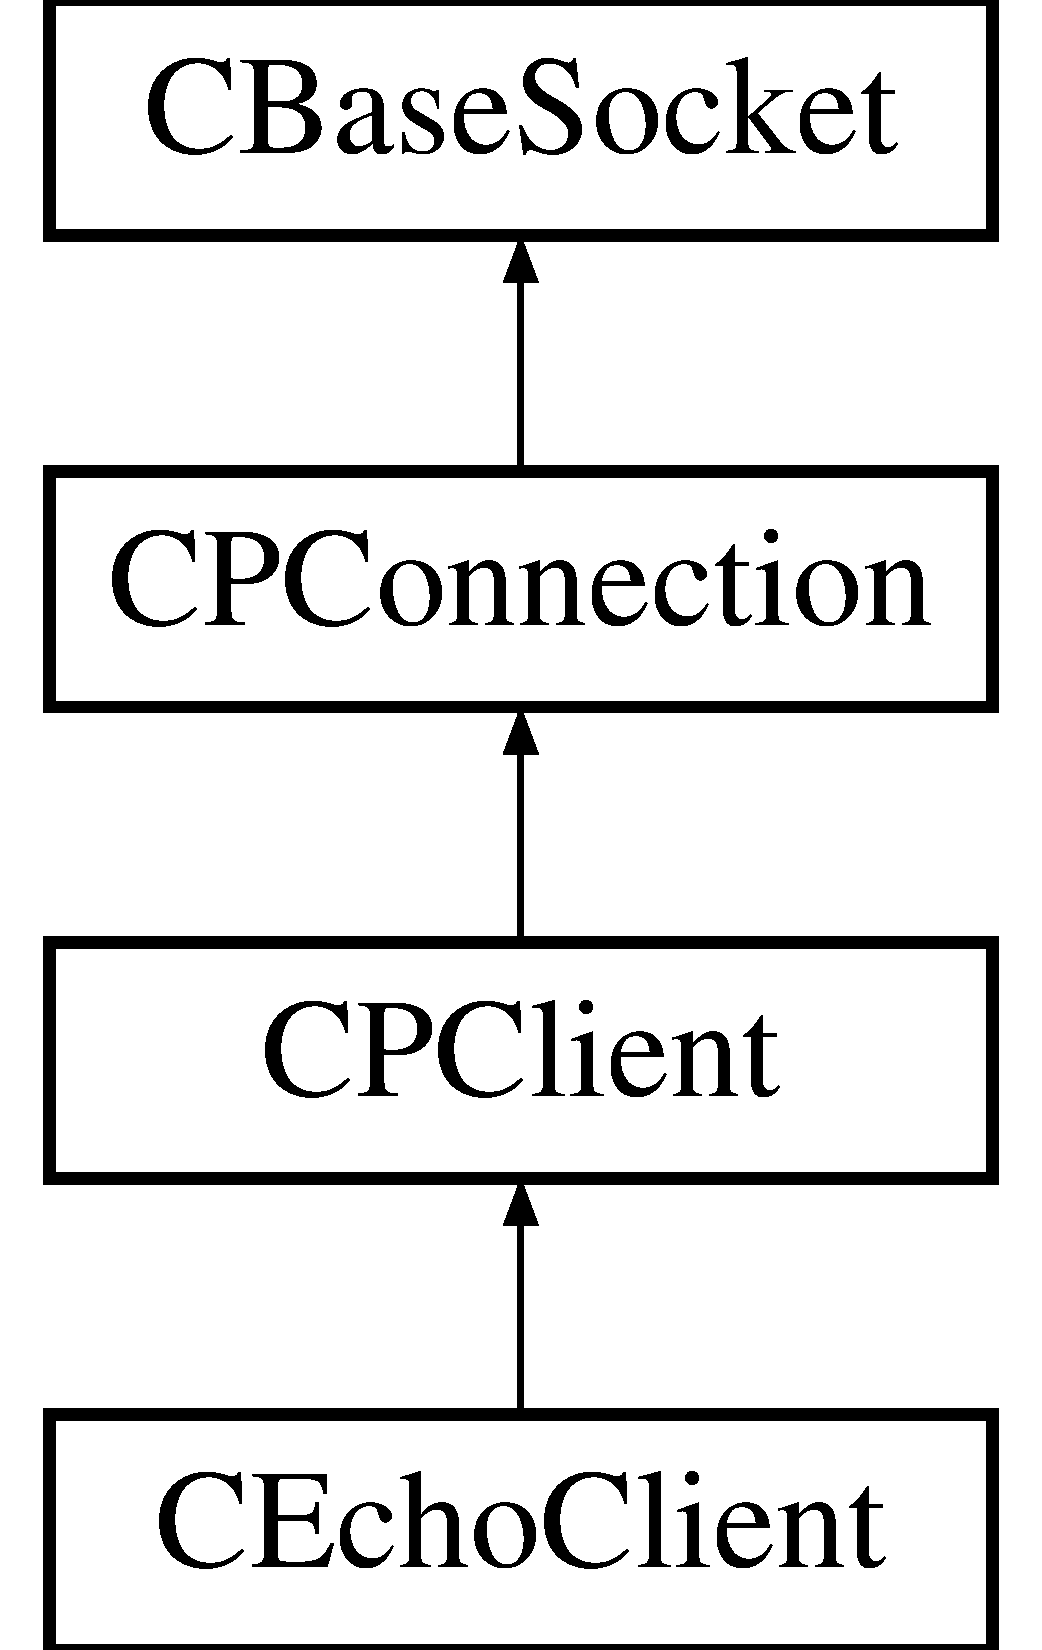
\includegraphics[height=4.000000cm]{class_c_p_client}
\end{center}
\end{figure}
\subsection*{\-Public \-Member \-Functions}
\begin{DoxyCompactItemize}
\item 
\hyperlink{class_c_p_client_aa5be4005f9e2cafc97ae40e28ea0bda7}{\-C\-P\-Client} (\hyperlink{_c_p_connection_handler_8h_a05bf2fef946dbf14350a5f45bb28f953}{\-C\-P\-\_\-\-C\-O\-N\-N\-E\-C\-T\-I\-O\-N\-\_\-\-H\-A\-N\-D\-L\-E\-R\-\_\-\-A\-R\-R\-A\-Y} \&c\-P\-C\-Handlers, \hyperlink{_c_p_client_handler_8h_a9babc356867a188aa505ce2ce4a81c46}{\-C\-P\-\_\-\-C\-L\-I\-E\-N\-T\-\_\-\-H\-A\-N\-D\-L\-E\-R\-\_\-\-A\-R\-R\-A\-Y} \&c\-P\-Client\-Handlers, int i\-Max\-Send\-Buffer\-Size=16384)
\item 
virtual \hyperlink{class_c_p_client_a8100ec5a3ccf5a3bec05d20f6ba1a3da}{$\sim$\-C\-P\-Client} ()
\item 
virtual \hyperlink{_cpclient_8h_a3be13892ae7076009afcf121347dd319}{\-B\-O\-O\-L} \hyperlink{class_c_p_client_ab78ee2bb6fd59f830435f4d3241c25b2}{\-Connect\-To\-Server} (\hyperlink{_x_plat_8h_a2b72c6037793f6c6381a09c83f27569b}{\-L\-P\-C\-S\-T\-R} lpsz\-Host\-Address, \hyperlink{_x_plat_8h_a45c20c14d3d8790a22153d08ab2eb2ff}{\-U\-I\-N\-T} n\-Host\-Port, \hyperlink{_x_plat_8h_aa39b39d94407451a6ec0226479db68cf}{\-D\-W\-O\-R\-D} dw\-Timeout=\hyperlink{_x_plat_8h_aa84a29002ab81c719c0d07bb446296e0}{\-I\-N\-F\-I\-N\-I\-T\-E}, \hyperlink{_x_plat_8h_a2b72c6037793f6c6381a09c83f27569b}{\-L\-P\-C\-S\-T\-R} lpsz\-Client\-Address=\-N\-U\-L\-L)
\begin{DoxyCompactList}\small\item\em \-Attempt to connect to the server. \end{DoxyCompactList}\item 
virtual \hyperlink{_cpclient_8h_a3be13892ae7076009afcf121347dd319}{\-B\-O\-O\-L} \hyperlink{class_c_p_client_a503733405e241cade1bebf3a935b296f}{\-Async\-Connect\-To\-Server} (\-C\-P\-C\-L\-I\-E\-N\-T\-\_\-\-C\-A\-L\-L\-B\-A\-C\-K p\-User\-Func, \hyperlink{_cpclient_8h_a6464f7480a0fd0ee170cba12b2c0497f}{void} $\ast$\hyperlink{class_c_p_client_a4c7f8139f898544073f5e535d5022ae6}{p\-User\-Parm}, \hyperlink{_x_plat_8h_a2b72c6037793f6c6381a09c83f27569b}{\-L\-P\-C\-S\-T\-R} lpsz\-Host\-Address, \hyperlink{_x_plat_8h_a45c20c14d3d8790a22153d08ab2eb2ff}{\-U\-I\-N\-T} n\-Host\-Port, \hyperlink{_x_plat_8h_aa39b39d94407451a6ec0226479db68cf}{\-D\-W\-O\-R\-D} dw\-Timeout=\hyperlink{_x_plat_8h_aa84a29002ab81c719c0d07bb446296e0}{\-I\-N\-F\-I\-N\-I\-T\-E}, \hyperlink{_x_plat_8h_a2b72c6037793f6c6381a09c83f27569b}{\-L\-P\-C\-S\-T\-R} lpsz\-Client\-Address=\-N\-U\-L\-L)
\begin{DoxyCompactList}\small\item\em \-An asynchronous attempt to connect to the server. \end{DoxyCompactList}\item 
\hyperlink{_cpclient_8h_a6464f7480a0fd0ee170cba12b2c0497f}{void} \hyperlink{class_c_p_client_aea1f62c59dfd45e814e9734ece8b0ab8}{\-Disconnected} ()
\begin{DoxyCompactList}\small\item\em \-If you derive from this, be sure to call the \hyperlink{class_c_p_client_aea1f62c59dfd45e814e9734ece8b0ab8}{\-C\-P\-Client\-::\-Disconnected} in your derived method! \end{DoxyCompactList}\item 
int \hyperlink{class_c_p_client_ade37dcde8e52312539263265295b9740}{\-Get\-Connection\-Error} ()
\begin{DoxyCompactList}\small\item\em \-Get the last error. \end{DoxyCompactList}\end{DoxyCompactItemize}
\subsection*{\-Public \-Attributes}
\begin{DoxyCompactItemize}
\item 
\hyperlink{_cpclient_8h_a6464f7480a0fd0ee170cba12b2c0497f}{void} $\ast$ \hyperlink{class_c_p_client_a4c7f8139f898544073f5e535d5022ae6}{p\-User\-Parm}
\item 
long \hyperlink{class_c_p_client_aa5d2b8ddd7b8ba324be40578ed419c52}{l\-Connect\-Response}
\end{DoxyCompactItemize}
\subsection*{\-Protected \-Member \-Functions}
\begin{DoxyCompactItemize}
\item 
\hyperlink{_cpclient_8h_a6464f7480a0fd0ee170cba12b2c0497f}{void} \hyperlink{class_c_p_client_a164a717aa6aac79d279d76624366ebcb}{\-Instance\-Connect\-Callback} (\hyperlink{_cpclient_8h_a3be13892ae7076009afcf121347dd319}{\-B\-O\-O\-L} b\-Connect\-Result)
\begin{DoxyCompactList}\small\item\em \-Same as the callback below, but on an instance instead of global level. \end{DoxyCompactList}\item 
\hyperlink{_cpclient_8h_a6464f7480a0fd0ee170cba12b2c0497f}{void} \hyperlink{class_c_p_client_a455c754945a3637cf1efcaaae38f6ebc}{\-Get\-Last\-Connect\-Attempt\-Parms} (string \&s\-Host, int \&i\-Port)
\begin{DoxyCompactList}\small\item\em \-Get last connect attempt parameters. \end{DoxyCompactList}\end{DoxyCompactItemize}
\subsection*{\-Static \-Protected \-Member \-Functions}
\begin{DoxyCompactItemize}
\item 
static \hyperlink{_cpclient_8h_a6464f7480a0fd0ee170cba12b2c0497f}{void} \hyperlink{class_c_p_client_a03b094fc0dba18e2358a237dd2185b32}{\-Connect\-Callback} (\hyperlink{class_c_p_client}{\-C\-P\-Client} $\ast$p\-Client, \hyperlink{_cpclient_8h_a3be13892ae7076009afcf121347dd319}{\-B\-O\-O\-L} b\-Connect\-Result)
\begin{DoxyCompactList}\small\item\em \-Callback. \end{DoxyCompactList}\item 
static \hyperlink{_cpclient_8h_a6464f7480a0fd0ee170cba12b2c0497f}{void} \hyperlink{class_c_p_client_ab7da7a76df72c5fc8c281d3477d137b8}{\-Internal\-Callback} (\hyperlink{class_c_p_client}{\-C\-P\-Client} $\ast$p\-Client, \hyperlink{_cpclient_8h_a3be13892ae7076009afcf121347dd319}{\-B\-O\-O\-L} b\-Connect\-Result, \hyperlink{_cpclient_8h_a6464f7480a0fd0ee170cba12b2c0497f}{void} $\ast$)
\end{DoxyCompactItemize}
\subsection*{\-Protected \-Attributes}
\begin{DoxyCompactItemize}
\item 
\hyperlink{_c_p_client_handler_8h_a9babc356867a188aa505ce2ce4a81c46}{\-C\-P\-\_\-\-C\-L\-I\-E\-N\-T\-\_\-\-H\-A\-N\-D\-L\-E\-R\-\_\-\-A\-R\-R\-A\-Y} \hyperlink{class_c_p_client_a475af425d617e19f2cd382cfcc6ac063}{c\-Client\-Handlers}
\begin{DoxyCompactList}\small\item\em \-Array of \-C\-P\-Client\-Handlers using for making connections. \end{DoxyCompactList}\item 
int \hyperlink{class_c_p_client_a7299daff3cd3437159533c9011ff96a0}{i\-Num\-Client\-Handlers}
\item 
\hyperlink{_c_p_connection_handler_8h_a05bf2fef946dbf14350a5f45bb28f953}{\-C\-P\-\_\-\-C\-O\-N\-N\-E\-C\-T\-I\-O\-N\-\_\-\-H\-A\-N\-D\-L\-E\-R\-\_\-\-A\-R\-R\-A\-Y} \hyperlink{class_c_p_client_a56e74ec04a07eeaa6761cffdc7ce7e88}{c\-Connection\-Handlers}
\begin{DoxyCompactList}\small\item\em \-Array of \-C\-P\-Connection\-Handlers. \-Used for servicing successful connetions. \end{DoxyCompactList}\item 
int \hyperlink{class_c_p_client_a5a9c9fb8e3e0c1faee5c9740fab8c8e7}{i\-Num\-Conn\-Handlers}
\item 
\hyperlink{class_c_x_plat_event}{\-C\-X\-Plat\-Event} \hyperlink{class_c_p_client_ad3f5a757a62ce581acb07cbb74deebe0}{c\-Connected\-Event}
\begin{DoxyCompactList}\small\item\em \-Set when success or failure. \end{DoxyCompactList}\item 
unsigned long \hyperlink{class_c_p_client_a84c9b4e693df05ea1e4e0621d97ba6e7}{ul\-Attempt\-T\-S}
\begin{DoxyCompactList}\small\item\em \-Timestamp when the attempt started. \end{DoxyCompactList}\item 
\-C\-P\-C\-L\-I\-E\-N\-T\-\_\-\-C\-A\-L\-L\-B\-A\-C\-K \hyperlink{class_c_p_client_a4ebdee1edb46b01abdc6a813d709b0b3}{p\-C\-P\-L\-Func}
\begin{DoxyCompactList}\small\item\em \-User callback function. \end{DoxyCompactList}\item 
\hyperlink{_cpclient_8h_a6464f7480a0fd0ee170cba12b2c0497f}{void} $\ast$ \hyperlink{class_c_p_client_a5eb090c6230b60ebcaf56228746af7f0}{p\-User\-Connect\-Parm}
\item 
unsigned long \hyperlink{class_c_p_client_a67a9b34f71126762d953ce9911ba8524}{ul\-Timeout}
\item 
int \hyperlink{class_c_p_client_a23443904277d6b94147cdc8edf42b725}{i\-Connect\-Error}
\item 
string \hyperlink{class_c_p_client_ac07c25a192add6cf72a751608e1891ad}{s\-Last\-Host}
\item 
int \hyperlink{class_c_p_client_a8579466cb047a99e4e3baa735274fb8f}{i\-Last\-Port}
\item 
long \hyperlink{class_c_p_client_a8d8282a0802a5d2cc96da57905fa9f81}{l\-Start\-Time}
\item 
string \hyperlink{class_c_p_client_a0b054ae566dabb8b7a794f8d53aec83a}{s\-Server}
\end{DoxyCompactItemize}


\subsection{\-Detailed \-Description}
\-Initiate a \-T\-C\-P client connection. 

\-Definition at line 40 of file \-Cpclient.\-h.



\subsection{\-Constructor \& \-Destructor \-Documentation}
\hypertarget{class_c_p_client_aa5be4005f9e2cafc97ae40e28ea0bda7}{\index{\-C\-P\-Client@{\-C\-P\-Client}!\-C\-P\-Client@{\-C\-P\-Client}}
\index{\-C\-P\-Client@{\-C\-P\-Client}!CPClient@{\-C\-P\-Client}}
\subsubsection[{\-C\-P\-Client}]{\setlength{\rightskip}{0pt plus 5cm}{\bf \-C\-P\-Client\-::\-C\-P\-Client} (
\begin{DoxyParamCaption}
\item[{{\bf \-C\-P\-\_\-\-C\-O\-N\-N\-E\-C\-T\-I\-O\-N\-\_\-\-H\-A\-N\-D\-L\-E\-R\-\_\-\-A\-R\-R\-A\-Y} \&}]{c\-P\-C\-Handlers, }
\item[{{\bf \-C\-P\-\_\-\-C\-L\-I\-E\-N\-T\-\_\-\-H\-A\-N\-D\-L\-E\-R\-\_\-\-A\-R\-R\-A\-Y} \&}]{c\-P\-Client\-Handlers, }
\item[{int}]{i\-Max\-Send\-Buffer\-Size = {\ttfamily 16384}}
\end{DoxyParamCaption}
)}}\label{class_c_p_client_aa5be4005f9e2cafc97ae40e28ea0bda7}


\-Definition at line 27 of file \-Cpclient.\-cpp.

\hypertarget{class_c_p_client_a8100ec5a3ccf5a3bec05d20f6ba1a3da}{\index{\-C\-P\-Client@{\-C\-P\-Client}!$\sim$\-C\-P\-Client@{$\sim$\-C\-P\-Client}}
\index{$\sim$\-C\-P\-Client@{$\sim$\-C\-P\-Client}!CPClient@{\-C\-P\-Client}}
\subsubsection[{$\sim$\-C\-P\-Client}]{\setlength{\rightskip}{0pt plus 5cm}{\bf \-C\-P\-Client\-::$\sim$\-C\-P\-Client} (
\begin{DoxyParamCaption}
{}
\end{DoxyParamCaption}
)\hspace{0.3cm}{\ttfamily  \mbox{[}virtual\mbox{]}}}}\label{class_c_p_client_a8100ec5a3ccf5a3bec05d20f6ba1a3da}


\-Definition at line 39 of file \-Cpclient.\-cpp.



\subsection{\-Member \-Function \-Documentation}
\hypertarget{class_c_p_client_a503733405e241cade1bebf3a935b296f}{\index{\-C\-P\-Client@{\-C\-P\-Client}!\-Async\-Connect\-To\-Server@{\-Async\-Connect\-To\-Server}}
\index{\-Async\-Connect\-To\-Server@{\-Async\-Connect\-To\-Server}!CPClient@{\-C\-P\-Client}}
\subsubsection[{\-Async\-Connect\-To\-Server}]{\setlength{\rightskip}{0pt plus 5cm}{\bf \-B\-O\-O\-L} {\bf \-C\-P\-Client\-::\-Async\-Connect\-To\-Server} (
\begin{DoxyParamCaption}
\item[{\-C\-P\-C\-L\-I\-E\-N\-T\-\_\-\-C\-A\-L\-L\-B\-A\-C\-K}]{p\-User\-Func, }
\item[{{\bf void} $\ast$}]{p\-User\-Parm, }
\item[{{\bf \-L\-P\-C\-S\-T\-R}}]{lpsz\-Host\-Address, }
\item[{{\bf \-U\-I\-N\-T}}]{n\-Host\-Port, }
\item[{{\bf \-D\-W\-O\-R\-D}}]{dw\-Timeout = {\ttfamily {\bf \-I\-N\-F\-I\-N\-I\-T\-E}}, }
\item[{{\bf \-L\-P\-C\-S\-T\-R}}]{lpsz\-Client\-Address = {\ttfamily \-N\-U\-L\-L}}
\end{DoxyParamCaption}
)\hspace{0.3cm}{\ttfamily  \mbox{[}virtual\mbox{]}}}}\label{class_c_p_client_a503733405e241cade1bebf3a935b296f}


\-An asynchronous attempt to connect to the server. 



\-Definition at line 72 of file \-Cpclient.\-cpp.

\hypertarget{class_c_p_client_a03b094fc0dba18e2358a237dd2185b32}{\index{\-C\-P\-Client@{\-C\-P\-Client}!\-Connect\-Callback@{\-Connect\-Callback}}
\index{\-Connect\-Callback@{\-Connect\-Callback}!CPClient@{\-C\-P\-Client}}
\subsubsection[{\-Connect\-Callback}]{\setlength{\rightskip}{0pt plus 5cm}{\bf void} {\bf \-C\-P\-Client\-::\-Connect\-Callback} (
\begin{DoxyParamCaption}
\item[{{\bf \-C\-P\-Client} $\ast$}]{p\-Client, }
\item[{{\bf \-B\-O\-O\-L}}]{b\-Connect\-Result}
\end{DoxyParamCaption}
)\hspace{0.3cm}{\ttfamily  \mbox{[}static, protected\mbox{]}}}}\label{class_c_p_client_a03b094fc0dba18e2358a237dd2185b32}


\-Callback. 



\-Definition at line 218 of file \-Cpclient.\-cpp.

\hypertarget{class_c_p_client_ab78ee2bb6fd59f830435f4d3241c25b2}{\index{\-C\-P\-Client@{\-C\-P\-Client}!\-Connect\-To\-Server@{\-Connect\-To\-Server}}
\index{\-Connect\-To\-Server@{\-Connect\-To\-Server}!CPClient@{\-C\-P\-Client}}
\subsubsection[{\-Connect\-To\-Server}]{\setlength{\rightskip}{0pt plus 5cm}{\bf \-B\-O\-O\-L} {\bf \-C\-P\-Client\-::\-Connect\-To\-Server} (
\begin{DoxyParamCaption}
\item[{{\bf \-L\-P\-C\-S\-T\-R}}]{lpsz\-Host\-Address, }
\item[{{\bf \-U\-I\-N\-T}}]{n\-Host\-Port, }
\item[{{\bf \-D\-W\-O\-R\-D}}]{dw\-Timeout = {\ttfamily {\bf \-I\-N\-F\-I\-N\-I\-T\-E}}, }
\item[{{\bf \-L\-P\-C\-S\-T\-R}}]{lpsz\-Client\-Address = {\ttfamily \-N\-U\-L\-L}}
\end{DoxyParamCaption}
)\hspace{0.3cm}{\ttfamily  \mbox{[}virtual\mbox{]}}}}\label{class_c_p_client_ab78ee2bb6fd59f830435f4d3241c25b2}


\-Attempt to connect to the server. 



\-Definition at line 45 of file \-Cpclient.\-cpp.

\hypertarget{class_c_p_client_aea1f62c59dfd45e814e9734ece8b0ab8}{\index{\-C\-P\-Client@{\-C\-P\-Client}!\-Disconnected@{\-Disconnected}}
\index{\-Disconnected@{\-Disconnected}!CPClient@{\-C\-P\-Client}}
\subsubsection[{\-Disconnected}]{\setlength{\rightskip}{0pt plus 5cm}{\bf void} {\bf \-C\-P\-Client\-::\-Disconnected} (
\begin{DoxyParamCaption}
{}
\end{DoxyParamCaption}
)\hspace{0.3cm}{\ttfamily  \mbox{[}virtual\mbox{]}}}}\label{class_c_p_client_aea1f62c59dfd45e814e9734ece8b0ab8}


\-If you derive from this, be sure to call the \hyperlink{class_c_p_client_aea1f62c59dfd45e814e9734ece8b0ab8}{\-C\-P\-Client\-::\-Disconnected} in your derived method! 



\-Reimplemented from \hyperlink{class_c_p_connection_a331c50e83d37b88ac099aa95b6b1523c}{\-C\-P\-Connection}.



\-Definition at line 225 of file \-Cpclient.\-cpp.

\hypertarget{class_c_p_client_ade37dcde8e52312539263265295b9740}{\index{\-C\-P\-Client@{\-C\-P\-Client}!\-Get\-Connection\-Error@{\-Get\-Connection\-Error}}
\index{\-Get\-Connection\-Error@{\-Get\-Connection\-Error}!CPClient@{\-C\-P\-Client}}
\subsubsection[{\-Get\-Connection\-Error}]{\setlength{\rightskip}{0pt plus 5cm}int {\bf \-C\-P\-Client\-::\-Get\-Connection\-Error} (
\begin{DoxyParamCaption}
{}
\end{DoxyParamCaption}
)}}\label{class_c_p_client_ade37dcde8e52312539263265295b9740}


\-Get the last error. 



\-Definition at line 232 of file \-Cpclient.\-cpp.

\hypertarget{class_c_p_client_a455c754945a3637cf1efcaaae38f6ebc}{\index{\-C\-P\-Client@{\-C\-P\-Client}!\-Get\-Last\-Connect\-Attempt\-Parms@{\-Get\-Last\-Connect\-Attempt\-Parms}}
\index{\-Get\-Last\-Connect\-Attempt\-Parms@{\-Get\-Last\-Connect\-Attempt\-Parms}!CPClient@{\-C\-P\-Client}}
\subsubsection[{\-Get\-Last\-Connect\-Attempt\-Parms}]{\setlength{\rightskip}{0pt plus 5cm}{\bf void} {\bf \-C\-P\-Client\-::\-Get\-Last\-Connect\-Attempt\-Parms} (
\begin{DoxyParamCaption}
\item[{string \&}]{s\-Host, }
\item[{int \&}]{i\-Port}
\end{DoxyParamCaption}
)\hspace{0.3cm}{\ttfamily  \mbox{[}protected\mbox{]}}}}\label{class_c_p_client_a455c754945a3637cf1efcaaae38f6ebc}


\-Get last connect attempt parameters. 



\-Definition at line 239 of file \-Cpclient.\-cpp.

\hypertarget{class_c_p_client_a164a717aa6aac79d279d76624366ebcb}{\index{\-C\-P\-Client@{\-C\-P\-Client}!\-Instance\-Connect\-Callback@{\-Instance\-Connect\-Callback}}
\index{\-Instance\-Connect\-Callback@{\-Instance\-Connect\-Callback}!CPClient@{\-C\-P\-Client}}
\subsubsection[{\-Instance\-Connect\-Callback}]{\setlength{\rightskip}{0pt plus 5cm}{\bf void} {\bf \-C\-P\-Client\-::\-Instance\-Connect\-Callback} (
\begin{DoxyParamCaption}
\item[{{\bf \-B\-O\-O\-L}}]{b\-Connect\-Result}
\end{DoxyParamCaption}
)\hspace{0.3cm}{\ttfamily  \mbox{[}protected\mbox{]}}}}\label{class_c_p_client_a164a717aa6aac79d279d76624366ebcb}


\-Same as the callback below, but on an instance instead of global level. 



\-Definition at line 175 of file \-Cpclient.\-cpp.

\hypertarget{class_c_p_client_ab7da7a76df72c5fc8c281d3477d137b8}{\index{\-C\-P\-Client@{\-C\-P\-Client}!\-Internal\-Callback@{\-Internal\-Callback}}
\index{\-Internal\-Callback@{\-Internal\-Callback}!CPClient@{\-C\-P\-Client}}
\subsubsection[{\-Internal\-Callback}]{\setlength{\rightskip}{0pt plus 5cm}{\bf void} {\bf \-C\-P\-Client\-::\-Internal\-Callback} (
\begin{DoxyParamCaption}
\item[{{\bf \-C\-P\-Client} $\ast$}]{p\-Client, }
\item[{{\bf \-B\-O\-O\-L}}]{b\-Connect\-Result, }
\item[{{\bf void} $\ast$}]{}
\end{DoxyParamCaption}
)\hspace{0.3cm}{\ttfamily  \mbox{[}static, protected\mbox{]}}}}\label{class_c_p_client_ab7da7a76df72c5fc8c281d3477d137b8}


\-Definition at line 247 of file \-Cpclient.\-cpp.



\subsection{\-Member \-Data \-Documentation}
\hypertarget{class_c_p_client_a475af425d617e19f2cd382cfcc6ac063}{\index{\-C\-P\-Client@{\-C\-P\-Client}!c\-Client\-Handlers@{c\-Client\-Handlers}}
\index{c\-Client\-Handlers@{c\-Client\-Handlers}!CPClient@{\-C\-P\-Client}}
\subsubsection[{c\-Client\-Handlers}]{\setlength{\rightskip}{0pt plus 5cm}{\bf \-C\-P\-\_\-\-C\-L\-I\-E\-N\-T\-\_\-\-H\-A\-N\-D\-L\-E\-R\-\_\-\-A\-R\-R\-A\-Y} {\bf \-C\-P\-Client\-::c\-Client\-Handlers}\hspace{0.3cm}{\ttfamily  \mbox{[}protected\mbox{]}}}}\label{class_c_p_client_a475af425d617e19f2cd382cfcc6ac063}


\-Array of \-C\-P\-Client\-Handlers using for making connections. 



\-Definition at line 86 of file \-Cpclient.\-h.

\hypertarget{class_c_p_client_ad3f5a757a62ce581acb07cbb74deebe0}{\index{\-C\-P\-Client@{\-C\-P\-Client}!c\-Connected\-Event@{c\-Connected\-Event}}
\index{c\-Connected\-Event@{c\-Connected\-Event}!CPClient@{\-C\-P\-Client}}
\subsubsection[{c\-Connected\-Event}]{\setlength{\rightskip}{0pt plus 5cm}{\bf \-C\-X\-Plat\-Event} {\bf \-C\-P\-Client\-::c\-Connected\-Event}\hspace{0.3cm}{\ttfamily  \mbox{[}protected\mbox{]}}}}\label{class_c_p_client_ad3f5a757a62ce581acb07cbb74deebe0}


\-Set when success or failure. 



\-Definition at line 92 of file \-Cpclient.\-h.

\hypertarget{class_c_p_client_a56e74ec04a07eeaa6761cffdc7ce7e88}{\index{\-C\-P\-Client@{\-C\-P\-Client}!c\-Connection\-Handlers@{c\-Connection\-Handlers}}
\index{c\-Connection\-Handlers@{c\-Connection\-Handlers}!CPClient@{\-C\-P\-Client}}
\subsubsection[{c\-Connection\-Handlers}]{\setlength{\rightskip}{0pt plus 5cm}{\bf \-C\-P\-\_\-\-C\-O\-N\-N\-E\-C\-T\-I\-O\-N\-\_\-\-H\-A\-N\-D\-L\-E\-R\-\_\-\-A\-R\-R\-A\-Y} {\bf \-C\-P\-Client\-::c\-Connection\-Handlers}\hspace{0.3cm}{\ttfamily  \mbox{[}protected\mbox{]}}}}\label{class_c_p_client_a56e74ec04a07eeaa6761cffdc7ce7e88}


\-Array of \-C\-P\-Connection\-Handlers. \-Used for servicing successful connetions. 



\-Definition at line 89 of file \-Cpclient.\-h.

\hypertarget{class_c_p_client_a23443904277d6b94147cdc8edf42b725}{\index{\-C\-P\-Client@{\-C\-P\-Client}!i\-Connect\-Error@{i\-Connect\-Error}}
\index{i\-Connect\-Error@{i\-Connect\-Error}!CPClient@{\-C\-P\-Client}}
\subsubsection[{i\-Connect\-Error}]{\setlength{\rightskip}{0pt plus 5cm}int {\bf \-C\-P\-Client\-::i\-Connect\-Error}\hspace{0.3cm}{\ttfamily  \mbox{[}protected\mbox{]}}}}\label{class_c_p_client_a23443904277d6b94147cdc8edf42b725}


\-Definition at line 99 of file \-Cpclient.\-h.

\hypertarget{class_c_p_client_a8579466cb047a99e4e3baa735274fb8f}{\index{\-C\-P\-Client@{\-C\-P\-Client}!i\-Last\-Port@{i\-Last\-Port}}
\index{i\-Last\-Port@{i\-Last\-Port}!CPClient@{\-C\-P\-Client}}
\subsubsection[{i\-Last\-Port}]{\setlength{\rightskip}{0pt plus 5cm}int {\bf \-C\-P\-Client\-::i\-Last\-Port}\hspace{0.3cm}{\ttfamily  \mbox{[}protected\mbox{]}}}}\label{class_c_p_client_a8579466cb047a99e4e3baa735274fb8f}


\-Definition at line 101 of file \-Cpclient.\-h.

\hypertarget{class_c_p_client_a7299daff3cd3437159533c9011ff96a0}{\index{\-C\-P\-Client@{\-C\-P\-Client}!i\-Num\-Client\-Handlers@{i\-Num\-Client\-Handlers}}
\index{i\-Num\-Client\-Handlers@{i\-Num\-Client\-Handlers}!CPClient@{\-C\-P\-Client}}
\subsubsection[{i\-Num\-Client\-Handlers}]{\setlength{\rightskip}{0pt plus 5cm}int {\bf \-C\-P\-Client\-::i\-Num\-Client\-Handlers}\hspace{0.3cm}{\ttfamily  \mbox{[}protected\mbox{]}}}}\label{class_c_p_client_a7299daff3cd3437159533c9011ff96a0}


\-Definition at line 87 of file \-Cpclient.\-h.

\hypertarget{class_c_p_client_a5a9c9fb8e3e0c1faee5c9740fab8c8e7}{\index{\-C\-P\-Client@{\-C\-P\-Client}!i\-Num\-Conn\-Handlers@{i\-Num\-Conn\-Handlers}}
\index{i\-Num\-Conn\-Handlers@{i\-Num\-Conn\-Handlers}!CPClient@{\-C\-P\-Client}}
\subsubsection[{i\-Num\-Conn\-Handlers}]{\setlength{\rightskip}{0pt plus 5cm}int {\bf \-C\-P\-Client\-::i\-Num\-Conn\-Handlers}\hspace{0.3cm}{\ttfamily  \mbox{[}protected\mbox{]}}}}\label{class_c_p_client_a5a9c9fb8e3e0c1faee5c9740fab8c8e7}


\-Definition at line 90 of file \-Cpclient.\-h.

\hypertarget{class_c_p_client_aa5d2b8ddd7b8ba324be40578ed419c52}{\index{\-C\-P\-Client@{\-C\-P\-Client}!l\-Connect\-Response@{l\-Connect\-Response}}
\index{l\-Connect\-Response@{l\-Connect\-Response}!CPClient@{\-C\-P\-Client}}
\subsubsection[{l\-Connect\-Response}]{\setlength{\rightskip}{0pt plus 5cm}long {\bf \-C\-P\-Client\-::l\-Connect\-Response}}}\label{class_c_p_client_aa5d2b8ddd7b8ba324be40578ed419c52}


\-Definition at line 82 of file \-Cpclient.\-h.

\hypertarget{class_c_p_client_a8d8282a0802a5d2cc96da57905fa9f81}{\index{\-C\-P\-Client@{\-C\-P\-Client}!l\-Start\-Time@{l\-Start\-Time}}
\index{l\-Start\-Time@{l\-Start\-Time}!CPClient@{\-C\-P\-Client}}
\subsubsection[{l\-Start\-Time}]{\setlength{\rightskip}{0pt plus 5cm}long {\bf \-C\-P\-Client\-::l\-Start\-Time}\hspace{0.3cm}{\ttfamily  \mbox{[}protected\mbox{]}}}}\label{class_c_p_client_a8d8282a0802a5d2cc96da57905fa9f81}


\-Definition at line 102 of file \-Cpclient.\-h.

\hypertarget{class_c_p_client_a4ebdee1edb46b01abdc6a813d709b0b3}{\index{\-C\-P\-Client@{\-C\-P\-Client}!p\-C\-P\-L\-Func@{p\-C\-P\-L\-Func}}
\index{p\-C\-P\-L\-Func@{p\-C\-P\-L\-Func}!CPClient@{\-C\-P\-Client}}
\subsubsection[{p\-C\-P\-L\-Func}]{\setlength{\rightskip}{0pt plus 5cm}\-C\-P\-C\-L\-I\-E\-N\-T\-\_\-\-C\-A\-L\-L\-B\-A\-C\-K {\bf \-C\-P\-Client\-::p\-C\-P\-L\-Func}\hspace{0.3cm}{\ttfamily  \mbox{[}protected\mbox{]}}}}\label{class_c_p_client_a4ebdee1edb46b01abdc6a813d709b0b3}


\-User callback function. 



\-Definition at line 96 of file \-Cpclient.\-h.

\hypertarget{class_c_p_client_a5eb090c6230b60ebcaf56228746af7f0}{\index{\-C\-P\-Client@{\-C\-P\-Client}!p\-User\-Connect\-Parm@{p\-User\-Connect\-Parm}}
\index{p\-User\-Connect\-Parm@{p\-User\-Connect\-Parm}!CPClient@{\-C\-P\-Client}}
\subsubsection[{p\-User\-Connect\-Parm}]{\setlength{\rightskip}{0pt plus 5cm}{\bf void}$\ast$ {\bf \-C\-P\-Client\-::p\-User\-Connect\-Parm}\hspace{0.3cm}{\ttfamily  \mbox{[}protected\mbox{]}}}}\label{class_c_p_client_a5eb090c6230b60ebcaf56228746af7f0}


\-Definition at line 97 of file \-Cpclient.\-h.

\hypertarget{class_c_p_client_a4c7f8139f898544073f5e535d5022ae6}{\index{\-C\-P\-Client@{\-C\-P\-Client}!p\-User\-Parm@{p\-User\-Parm}}
\index{p\-User\-Parm@{p\-User\-Parm}!CPClient@{\-C\-P\-Client}}
\subsubsection[{p\-User\-Parm}]{\setlength{\rightskip}{0pt plus 5cm}{\bf void}$\ast$ {\bf \-C\-P\-Client\-::p\-User\-Parm}}}\label{class_c_p_client_a4c7f8139f898544073f5e535d5022ae6}


\-Definition at line 81 of file \-Cpclient.\-h.

\hypertarget{class_c_p_client_ac07c25a192add6cf72a751608e1891ad}{\index{\-C\-P\-Client@{\-C\-P\-Client}!s\-Last\-Host@{s\-Last\-Host}}
\index{s\-Last\-Host@{s\-Last\-Host}!CPClient@{\-C\-P\-Client}}
\subsubsection[{s\-Last\-Host}]{\setlength{\rightskip}{0pt plus 5cm}string {\bf \-C\-P\-Client\-::s\-Last\-Host}\hspace{0.3cm}{\ttfamily  \mbox{[}protected\mbox{]}}}}\label{class_c_p_client_ac07c25a192add6cf72a751608e1891ad}


\-Definition at line 100 of file \-Cpclient.\-h.

\hypertarget{class_c_p_client_a0b054ae566dabb8b7a794f8d53aec83a}{\index{\-C\-P\-Client@{\-C\-P\-Client}!s\-Server@{s\-Server}}
\index{s\-Server@{s\-Server}!CPClient@{\-C\-P\-Client}}
\subsubsection[{s\-Server}]{\setlength{\rightskip}{0pt plus 5cm}string {\bf \-C\-P\-Client\-::s\-Server}\hspace{0.3cm}{\ttfamily  \mbox{[}protected\mbox{]}}}}\label{class_c_p_client_a0b054ae566dabb8b7a794f8d53aec83a}


\-Definition at line 103 of file \-Cpclient.\-h.

\hypertarget{class_c_p_client_a84c9b4e693df05ea1e4e0621d97ba6e7}{\index{\-C\-P\-Client@{\-C\-P\-Client}!ul\-Attempt\-T\-S@{ul\-Attempt\-T\-S}}
\index{ul\-Attempt\-T\-S@{ul\-Attempt\-T\-S}!CPClient@{\-C\-P\-Client}}
\subsubsection[{ul\-Attempt\-T\-S}]{\setlength{\rightskip}{0pt plus 5cm}unsigned long {\bf \-C\-P\-Client\-::ul\-Attempt\-T\-S}\hspace{0.3cm}{\ttfamily  \mbox{[}protected\mbox{]}}}}\label{class_c_p_client_a84c9b4e693df05ea1e4e0621d97ba6e7}


\-Timestamp when the attempt started. 



\-Definition at line 94 of file \-Cpclient.\-h.

\hypertarget{class_c_p_client_a67a9b34f71126762d953ce9911ba8524}{\index{\-C\-P\-Client@{\-C\-P\-Client}!ul\-Timeout@{ul\-Timeout}}
\index{ul\-Timeout@{ul\-Timeout}!CPClient@{\-C\-P\-Client}}
\subsubsection[{ul\-Timeout}]{\setlength{\rightskip}{0pt plus 5cm}unsigned long {\bf \-C\-P\-Client\-::ul\-Timeout}\hspace{0.3cm}{\ttfamily  \mbox{[}protected\mbox{]}}}}\label{class_c_p_client_a67a9b34f71126762d953ce9911ba8524}


\-Definition at line 98 of file \-Cpclient.\-h.



\-The documentation for this class was generated from the following files\-:\begin{DoxyCompactItemize}
\item 
common/\hyperlink{_cpclient_8h}{\-Cpclient.\-h}\item 
common/\hyperlink{_cpclient_8cpp}{\-Cpclient.\-cpp}\end{DoxyCompactItemize}

\hypertarget{class_c_p_client_handler}{\section{\-C\-P\-Client\-Handler \-Class \-Reference}
\label{class_c_p_client_handler}\index{\-C\-P\-Client\-Handler@{\-C\-P\-Client\-Handler}}
}


{\ttfamily \#include $<$\-C\-P\-Client\-Handler.\-h$>$}

\-Inheritance diagram for \-C\-P\-Client\-Handler\-:\begin{figure}[H]
\begin{center}
\leavevmode
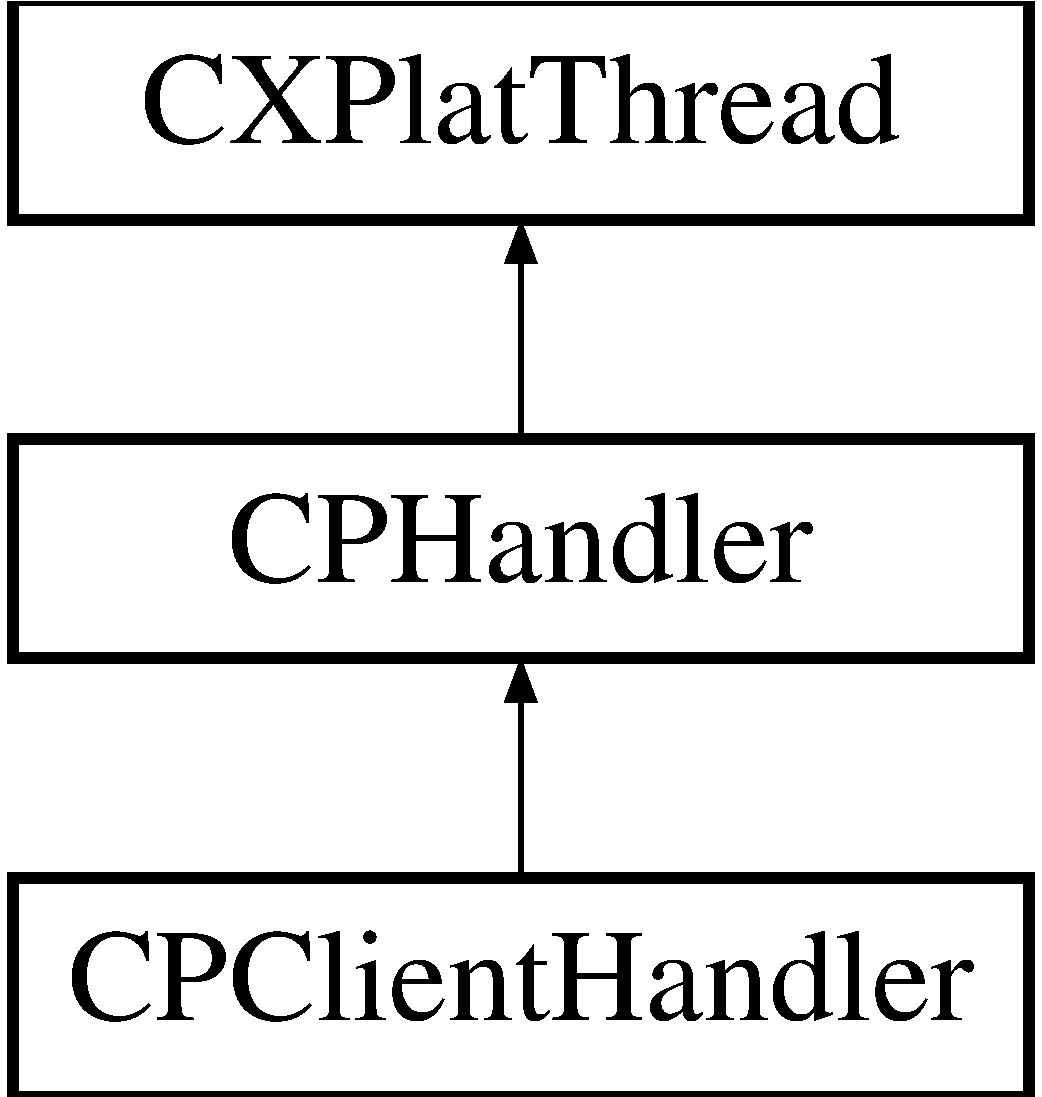
\includegraphics[height=3.000000cm]{class_c_p_client_handler}
\end{center}
\end{figure}
\subsection*{\-Public \-Member \-Functions}
\begin{DoxyCompactItemize}
\item 
\hyperlink{class_c_p_client_handler_a26b86af12546043f0079e1527fd420a6}{\-C\-P\-Client\-Handler} ()
\item 
virtual \hyperlink{class_c_p_client_handler_a3469cc970781324be0648feaca88b56c}{$\sim$\-C\-P\-Client\-Handler} ()
\item 
virtual int \hyperlink{class_c_p_client_handler_a7f6d153c5104840663b7225a36ea7609}{\-Call\-Handle\-Connection} (\hyperlink{class_c_p_connection}{\-C\-P\-Connection} $\ast$p\-Connection)
\end{DoxyCompactItemize}
\subsection*{\-Protected \-Member \-Functions}
\begin{DoxyCompactItemize}
\item 
virtual unsigned \hyperlink{class_c_p_client_handler_a88117dfe5e1e6d2f5d953277bc1a3044}{\-Worker\-Function} (\hyperlink{_cpclient_8h_a6464f7480a0fd0ee170cba12b2c0497f}{void} $\ast$p\-Param)
\begin{DoxyCompactList}\small\item\em \-Function that does the work. \end{DoxyCompactList}\item 
virtual \hyperlink{_cpclient_8h_a6464f7480a0fd0ee170cba12b2c0497f}{void} \hyperlink{class_c_p_client_handler_ad6df6ba23365c140780ddd27cb44bd08}{\-Call\-Disconnected} (\hyperlink{class_c_p_connection}{\-C\-P\-Connection} $\ast$p\-Connection)
\begin{DoxyCompactList}\small\item\em \-If we want to call the sockets \-Disconnected member. \end{DoxyCompactList}\end{DoxyCompactItemize}


\subsection{\-Detailed \-Description}
\-C\-P\-Clienthandler is a specialized \hyperlink{class_c_p_handler}{\-C\-P\-Handler} that acts as a \-T\-C\-P client, intiating a connection. 

\-Definition at line 38 of file \-C\-P\-Client\-Handler.\-h.



\subsection{\-Constructor \& \-Destructor \-Documentation}
\hypertarget{class_c_p_client_handler_a26b86af12546043f0079e1527fd420a6}{\index{\-C\-P\-Client\-Handler@{\-C\-P\-Client\-Handler}!\-C\-P\-Client\-Handler@{\-C\-P\-Client\-Handler}}
\index{\-C\-P\-Client\-Handler@{\-C\-P\-Client\-Handler}!CPClientHandler@{\-C\-P\-Client\-Handler}}
\subsubsection[{\-C\-P\-Client\-Handler}]{\setlength{\rightskip}{0pt plus 5cm}{\bf \-C\-P\-Client\-Handler\-::\-C\-P\-Client\-Handler} (
\begin{DoxyParamCaption}
{}
\end{DoxyParamCaption}
)}}\label{class_c_p_client_handler_a26b86af12546043f0079e1527fd420a6}


\-Definition at line 30 of file \-C\-P\-Client\-Handler.\-cpp.

\hypertarget{class_c_p_client_handler_a3469cc970781324be0648feaca88b56c}{\index{\-C\-P\-Client\-Handler@{\-C\-P\-Client\-Handler}!$\sim$\-C\-P\-Client\-Handler@{$\sim$\-C\-P\-Client\-Handler}}
\index{$\sim$\-C\-P\-Client\-Handler@{$\sim$\-C\-P\-Client\-Handler}!CPClientHandler@{\-C\-P\-Client\-Handler}}
\subsubsection[{$\sim$\-C\-P\-Client\-Handler}]{\setlength{\rightskip}{0pt plus 5cm}{\bf \-C\-P\-Client\-Handler\-::$\sim$\-C\-P\-Client\-Handler} (
\begin{DoxyParamCaption}
{}
\end{DoxyParamCaption}
)\hspace{0.3cm}{\ttfamily  \mbox{[}virtual\mbox{]}}}}\label{class_c_p_client_handler_a3469cc970781324be0648feaca88b56c}


\-Definition at line 39 of file \-C\-P\-Client\-Handler.\-cpp.



\subsection{\-Member \-Function \-Documentation}
\hypertarget{class_c_p_client_handler_ad6df6ba23365c140780ddd27cb44bd08}{\index{\-C\-P\-Client\-Handler@{\-C\-P\-Client\-Handler}!\-Call\-Disconnected@{\-Call\-Disconnected}}
\index{\-Call\-Disconnected@{\-Call\-Disconnected}!CPClientHandler@{\-C\-P\-Client\-Handler}}
\subsubsection[{\-Call\-Disconnected}]{\setlength{\rightskip}{0pt plus 5cm}virtual {\bf void} {\bf \-C\-P\-Client\-Handler\-::\-Call\-Disconnected} (
\begin{DoxyParamCaption}
\item[{{\bf \-C\-P\-Connection} $\ast$}]{p\-Connection}
\end{DoxyParamCaption}
)\hspace{0.3cm}{\ttfamily  \mbox{[}inline, protected, virtual\mbox{]}}}}\label{class_c_p_client_handler_ad6df6ba23365c140780ddd27cb44bd08}


\-If we want to call the sockets \-Disconnected member. 



\-Reimplemented from \hyperlink{class_c_p_handler_a439e2cfd01babb8ba9464a4300e90efe}{\-C\-P\-Handler}.



\-Definition at line 53 of file \-C\-P\-Client\-Handler.\-h.

\hypertarget{class_c_p_client_handler_a7f6d153c5104840663b7225a36ea7609}{\index{\-C\-P\-Client\-Handler@{\-C\-P\-Client\-Handler}!\-Call\-Handle\-Connection@{\-Call\-Handle\-Connection}}
\index{\-Call\-Handle\-Connection@{\-Call\-Handle\-Connection}!CPClientHandler@{\-C\-P\-Client\-Handler}}
\subsubsection[{\-Call\-Handle\-Connection}]{\setlength{\rightskip}{0pt plus 5cm}virtual int {\bf \-C\-P\-Client\-Handler\-::\-Call\-Handle\-Connection} (
\begin{DoxyParamCaption}
\item[{{\bf \-C\-P\-Connection} $\ast$}]{p\-Connection}
\end{DoxyParamCaption}
)\hspace{0.3cm}{\ttfamily  \mbox{[}inline, virtual\mbox{]}}}}\label{class_c_p_client_handler_a7f6d153c5104840663b7225a36ea7609}
\-Call the \-C\-P\-Connection-\/$>$\-Handle\-Connection \-This is here so derived classes can choose \-N\-O\-T to call it in case the handler is chained (like this one) 

\-Reimplemented from \hyperlink{class_c_p_handler_abe1898023c829d3af4b5d1c4efa89479}{\-C\-P\-Handler}.



\-Definition at line 47 of file \-C\-P\-Client\-Handler.\-h.

\hypertarget{class_c_p_client_handler_a88117dfe5e1e6d2f5d953277bc1a3044}{\index{\-C\-P\-Client\-Handler@{\-C\-P\-Client\-Handler}!\-Worker\-Function@{\-Worker\-Function}}
\index{\-Worker\-Function@{\-Worker\-Function}!CPClientHandler@{\-C\-P\-Client\-Handler}}
\subsubsection[{\-Worker\-Function}]{\setlength{\rightskip}{0pt plus 5cm}unsigned {\bf \-C\-P\-Client\-Handler\-::\-Worker\-Function} (
\begin{DoxyParamCaption}
\item[{{\bf void} $\ast$}]{p\-Param}
\end{DoxyParamCaption}
)\hspace{0.3cm}{\ttfamily  \mbox{[}protected, virtual\mbox{]}}}}\label{class_c_p_client_handler_a88117dfe5e1e6d2f5d953277bc1a3044}


\-Function that does the work. 



\-Implements \hyperlink{class_c_p_handler_a86df3a9d167e20ae405eec33e384bd9b}{\-C\-P\-Handler}.



\-Definition at line 45 of file \-C\-P\-Client\-Handler.\-cpp.



\-The documentation for this class was generated from the following files\-:\begin{DoxyCompactItemize}
\item 
common/\hyperlink{_c_p_client_handler_8h}{\-C\-P\-Client\-Handler.\-h}\item 
common/\hyperlink{_c_p_client_handler_8cpp}{\-C\-P\-Client\-Handler.\-cpp}\end{DoxyCompactItemize}

\hypertarget{class_c_p_connection}{\section{\-C\-P\-Connection \-Class \-Reference}
\label{class_c_p_connection}\index{\-C\-P\-Connection@{\-C\-P\-Connection}}
}


{\ttfamily \#include $<$\-C\-P\-Connection.\-h$>$}

\-Inheritance diagram for \-C\-P\-Connection\-:\begin{figure}[H]
\begin{center}
\leavevmode
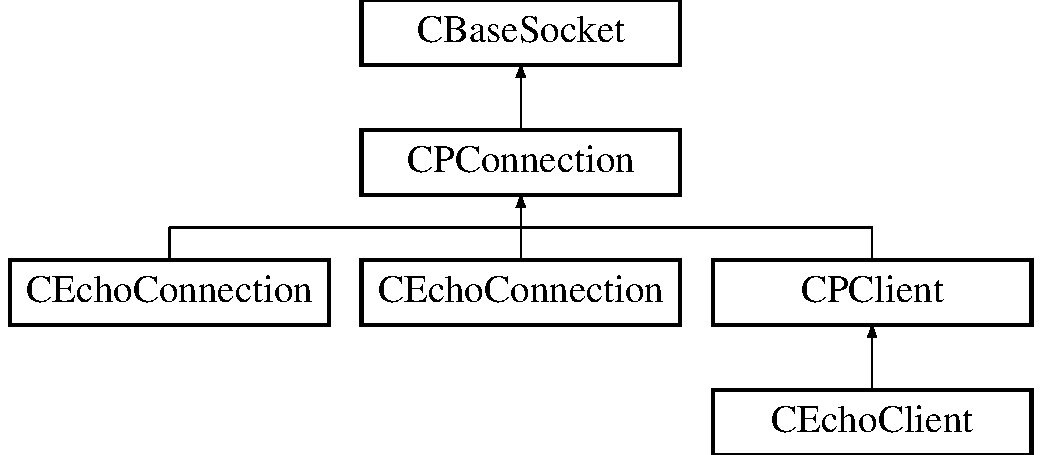
\includegraphics[height=4.000000cm]{class_c_p_connection}
\end{center}
\end{figure}
\subsection*{\-Public \-Types}
\begin{DoxyCompactItemize}
\item 
enum \{ \hyperlink{class_c_p_connection_a806d0ccf9284ab6cfa8f9f638df5b8e5a212b310ed9516ad4edce81eb3f615a90}{\-C\-S\-\_\-\-B\-U\-F\-F\-E\-R\-\_\-\-S\-I\-Z\-E} =  0x2000, 
\hyperlink{class_c_p_connection_a806d0ccf9284ab6cfa8f9f638df5b8e5ae1bfa53acfedd84586f9577402592e70}{\-C\-S\-\_\-\-O\-U\-T\-B\-U\-F\-F\-E\-R\-\_\-\-S\-I\-Z\-E} =  0x8000
 \}
\begin{DoxyCompactList}\small\item\em \-Operations. \end{DoxyCompactList}\item 
enum \hyperlink{class_c_p_connection_a0b9dfdba3bf3fb022507756c5eff7bde}{\-E\-C\-O\-N\-N\-E\-C\-T} \{ \*
\hyperlink{class_c_p_connection_a0b9dfdba3bf3fb022507756c5eff7bdeab33cb29fa6b86f5a9764b5a6ff6b9f98}{\-C\-O\-N\-N\-E\-C\-T\-\_\-\-U\-N\-U\-S\-E\-D}, 
\hyperlink{class_c_p_connection_a0b9dfdba3bf3fb022507756c5eff7bdeaa739beea3c36f54a1e48e309477fdecd}{\-C\-O\-N\-N\-E\-C\-T\-\_\-\-P\-E\-N\-D\-I\-N\-G}, 
\hyperlink{class_c_p_connection_a0b9dfdba3bf3fb022507756c5eff7bdead9adca01889d40665ea46c97029bf07b}{\-C\-O\-N\-N\-E\-C\-T\-\_\-\-A\-T\-T\-E\-M\-P\-T\-\_\-\-F\-A\-I\-L\-E\-D}, 
\hyperlink{class_c_p_connection_a0b9dfdba3bf3fb022507756c5eff7bdea414416c17cf4d03572ea886af634c463}{\-C\-O\-N\-N\-E\-C\-T\-\_\-\-S\-U\-C\-C\-E\-S\-S}, 
\*
\hyperlink{class_c_p_connection_a0b9dfdba3bf3fb022507756c5eff7bdea9a83b86ee125293f6d73d8afec74a145}{\-C\-O\-N\-N\-E\-C\-T\-\_\-\-C\-L\-O\-S\-E\-\_\-\-R\-E\-Q\-U\-E\-S\-T\-E\-D}, 
\hyperlink{class_c_p_connection_a0b9dfdba3bf3fb022507756c5eff7bdead12aa45cdb80e03a24de39dff800f4ae}{\-C\-O\-N\-N\-E\-C\-T\-\_\-\-D\-I\-S\-C\-O\-N\-N\-E\-C\-T\-E\-D}, 
\hyperlink{class_c_p_connection_a0b9dfdba3bf3fb022507756c5eff7bdeaf31728d4a1b415f3076875e6ac69053b}{\-C\-O\-N\-N\-E\-C\-T\-\_\-\-F\-A\-I\-L\-U\-R\-E}
 \}
\begin{DoxyCompactList}\small\item\em \-No public destructor. \end{DoxyCompactList}\end{DoxyCompactItemize}
\subsection*{\-Public \-Member \-Functions}
\begin{DoxyCompactItemize}
\item 
\hyperlink{class_c_p_connection_a512354ba23583d1bddc9cb4999d248f3}{\-C\-P\-Connection} (\hyperlink{class_c_base_socket}{\-C\-Base\-Socket} $\ast$p\-Owner, struct sockaddr $\ast$p\-Addr=\-N\-U\-L\-L, int i\-Max\-Send\-Buffer\-Size=\hyperlink{class_c_p_connection_a806d0ccf9284ab6cfa8f9f638df5b8e5ae1bfa53acfedd84586f9577402592e70}{\-C\-S\-\_\-\-O\-U\-T\-B\-U\-F\-F\-E\-R\-\_\-\-S\-I\-Z\-E})
\item 
virtual \hyperlink{class_c_p_connection_a7a06ca261e3c9418bf9cfe63bba8ad44}{$\sim$\-C\-P\-Connection} ()
\item 
virtual \hyperlink{_cpclient_8h_a3be13892ae7076009afcf121347dd319}{\-B\-O\-O\-L} \hyperlink{class_c_p_connection_a666a669dc7dfde6478fb599104cace44}{\-Create} (int af, int type, int protocol, \hyperlink{_x_plat_8h_a45c20c14d3d8790a22153d08ab2eb2ff}{\-U\-I\-N\-T} n\-Port=0, \hyperlink{_x_plat_8h_a2b72c6037793f6c6381a09c83f27569b}{\-L\-P\-C\-S\-T\-R} lp\-Addr=\-N\-U\-L\-L, \hyperlink{_cpclient_8h_a3be13892ae7076009afcf121347dd319}{\-B\-O\-O\-L} b\-Reuse=\hyperlink{_x_plat_8h_aa93f0eb578d23995850d61f7d61c55c1}{\-F\-A\-L\-S\-E}, \hyperlink{_cpclient_8h_a3be13892ae7076009afcf121347dd319}{\-B\-O\-O\-L} b\-Bind=\hyperlink{_x_plat_8h_aa8cecfc5c5c054d2875c03e77b7be15d}{\-T\-R\-U\-E}, int i\-Linger=-\/1)
\item 
virtual \hyperlink{_cpclient_8h_a6464f7480a0fd0ee170cba12b2c0497f}{void} \hyperlink{class_c_p_connection_a62d7805ad5ad95853f68628d5df4f0f1}{\-Terminate\-Connection} ()
\begin{DoxyCompactList}\small\item\em \-Terminate a connection and close the socket. \end{DoxyCompactList}\item 
virtual time\-\_\-t \hyperlink{class_c_p_connection_acbc1f976fdecf17d5d3b0b75b524d69c}{\-Get\-Time\-Connected} ()
\begin{DoxyCompactList}\small\item\em \-Return the time the connection was initiated. \end{DoxyCompactList}\item 
virtual struct sockaddr\-\_\-in \hyperlink{class_c_p_connection_a8a68ba35336e1255ae4c1e3bb77fb0e5}{\-Get\-Socket\-Address} ()
\begin{DoxyCompactList}\small\item\em \-Get socket address. \end{DoxyCompactList}\item 
virtual \hyperlink{_cpclient_8h_a6464f7480a0fd0ee170cba12b2c0497f}{void} \hyperlink{class_c_p_connection_a703a63596b3e3c93a8b76238bf5ec6f4}{\-Async\-Terminate\-Connection} ()
\item 
\hyperlink{class_c_p_connection_a0b9dfdba3bf3fb022507756c5eff7bde}{\-E\-C\-O\-N\-N\-E\-C\-T} \hyperlink{class_c_p_connection_a72266989e31085bfb2f45f603115a6fb}{\-Get\-Connection\-Status} ()
\begin{DoxyCompactList}\small\item\em \-Get connection status. \end{DoxyCompactList}\item 
\hyperlink{_cpclient_8h_a3be13892ae7076009afcf121347dd319}{\-B\-O\-O\-L} \hyperlink{class_c_p_connection_ae1ccbe730072cfaa3d5ad7d94c9d6571}{\-Is\-Send\-Complete} ()
\end{DoxyCompactItemize}
\subsection*{\-Public \-Attributes}
\begin{DoxyCompactItemize}
\item 
\hyperlink{_cpclient_8h_a3be13892ae7076009afcf121347dd319}{\-B\-O\-O\-L} \hyperlink{class_c_p_connection_aafe1dacf5a3a4927f44435e887b5e177}{b\-Recv\-Pause}
\end{DoxyCompactItemize}
\subsection*{\-Protected \-Member \-Functions}
\begin{DoxyCompactItemize}
\item 
virtual int \hyperlink{class_c_p_connection_a51cab90d3e5f74d43a838e4ed5fe9c89}{\-Receive\-Data} ()
\begin{DoxyCompactList}\small\item\em \-Receive the data to a socket. \end{DoxyCompactList}\item 
virtual int \hyperlink{class_c_p_connection_a7678a5c828e5bc52dd0619821904bcac}{\-Send\-Data} ()
\begin{DoxyCompactList}\small\item\em \-Send data from a socket. \end{DoxyCompactList}\item 
virtual \hyperlink{_cpclient_8h_a3be13892ae7076009afcf121347dd319}{\-B\-O\-O\-L} \hyperlink{class_c_p_connection_a502e914917ea8c82f2225253d1bd0a71}{\-Send\-Data\-Out} (\hyperlink{_x_plat_8h_ad162cb9da5f09788c88e33cd9486a158}{\-L\-P\-S\-T\-R} lp\-Data, int n\-Packet\-Size, int n\-Total\-Length)
\item 
virtual \hyperlink{_cpclient_8h_a3be13892ae7076009afcf121347dd319}{\-B\-O\-O\-L} \hyperlink{class_c_p_connection_a1b223eab8f518f390b2c01f7c1e33e72}{\-Process\-Data} (unsigned char $\ast$lp\-Data, int i\-Len)=0
\begin{DoxyCompactList}\small\item\em \-Pure virtual function to process data. \end{DoxyCompactList}\item 
virtual \hyperlink{_cpclient_8h_a3be13892ae7076009afcf121347dd319}{\-B\-O\-O\-L} \hyperlink{class_c_p_connection_a9793183adddb29f39186eee5eac6701f}{\-Get\-Handshake} (unsigned char $\ast$$\ast$uc\-H\-S, int \&i\-Len)
\item 
virtual \hyperlink{_cpclient_8h_a6464f7480a0fd0ee170cba12b2c0497f}{void} \hyperlink{class_c_p_connection_a331c50e83d37b88ac099aa95b6b1523c}{\-Disconnected} ()
\begin{DoxyCompactList}\small\item\em \-When removed from the handler, this gets called. \end{DoxyCompactList}\item 
virtual \hyperlink{_cpclient_8h_a6464f7480a0fd0ee170cba12b2c0497f}{void} \hyperlink{class_c_p_connection_a5c83da25150fd43d9fe4522d34d6cffb}{\-Unprotected\-Close\-Socket} ()
\begin{DoxyCompactList}\small\item\em \-Unprotected close socket. \end{DoxyCompactList}\item 
virtual \hyperlink{_cpclient_8h_a6464f7480a0fd0ee170cba12b2c0497f}{void} \hyperlink{class_c_p_connection_aea524e3f40bddc5ae1523fa16ae41622}{\-Set\-Handler} (\hyperlink{class_c_p_handler}{\-C\-P\-Handler} $\ast$p\-Handler)
\begin{DoxyCompactList}\small\item\em \-Called by the handler itself when it accepts the connection. \end{DoxyCompactList}\item 
virtual int \hyperlink{class_c_p_connection_aa25471c69703f9e8d8795dda25ba75ea}{\-Handle\-Connection} (\hyperlink{_cpclient_8h_a6464f7480a0fd0ee170cba12b2c0497f}{void} $\ast$p\-Parm=\-N\-U\-L\-L)
\end{DoxyCompactItemize}
\subsection*{\-Protected \-Attributes}
\begin{DoxyCompactItemize}
\item 
\hyperlink{class_c_p_handler}{\-C\-P\-Handler} $\ast$ \hyperlink{class_c_p_connection_a9e5914bdbd8aeabe9609d7aa8f03babe}{c\-P\-Handler}
\item 
int \hyperlink{class_c_p_connection_a5851cde8b69706593ef33933702e170a}{i\-Max\-Send\-Buffer}
\item 
unsigned char \hyperlink{class_c_p_connection_aa85421d2cbee8274c6794babc609dce6}{uc\-Buffer} \mbox{[}\hyperlink{class_c_p_connection_a806d0ccf9284ab6cfa8f9f638df5b8e5a212b310ed9516ad4edce81eb3f615a90}{\-C\-S\-\_\-\-B\-U\-F\-F\-E\-R\-\_\-\-S\-I\-Z\-E}\mbox{]}
\begin{DoxyCompactList}\small\item\em \-Input buffer. \end{DoxyCompactList}\item 
unsigned char $\ast$ \hyperlink{class_c_p_connection_a75a016a1c397b5646591eead6aabdfc5}{p\-Out\-Buffer}
\begin{DoxyCompactList}\small\item\em \-Output buffer. \end{DoxyCompactList}\item 
int \hyperlink{class_c_p_connection_a097c729d2ace3e54ad5c87264aac40e2}{i\-O\-B\-Size}
\begin{DoxyCompactList}\small\item\em \-Current size of the output buffer. \end{DoxyCompactList}\item 
int \hyperlink{class_c_p_connection_ac86d2db09fd1dc387c397b75ef491f6e}{i\-Left\-To\-Send}
\begin{DoxyCompactList}\small\item\em \-What's left to send in the out buffer. \end{DoxyCompactList}\item 
int \hyperlink{class_c_p_connection_aaac2a186e16efdb9f7786cc46dd81125}{i\-Send\-Index}
\begin{DoxyCompactList}\small\item\em \-Index of bytes to send. \end{DoxyCompactList}\item 
\hyperlink{class_c_base_socket}{\-C\-Base\-Socket} $\ast$ \hyperlink{class_c_p_connection_a504332c07c9fb47362b5c490182833e9}{c\-Owner}
\item 
time\-\_\-t \hyperlink{class_c_p_connection_a758401474fda32b364811b3ccbe2013f}{t\-Connected}
\item 
struct sockaddr\-\_\-in \hyperlink{class_c_p_connection_af5990e2eecbce8a899752e3f195c5cc1}{s\-Addr}
\item 
\hyperlink{_cpclient_8h_a3be13892ae7076009afcf121347dd319}{\-B\-O\-O\-L} \hyperlink{class_c_p_connection_ab1099445977c4cabbb67c86f6a0b9213}{b\-Send\-Data}
\begin{DoxyCompactList}\small\item\em \-There is data to be written. \end{DoxyCompactList}\item 
\hyperlink{_cpclient_8h_a3be13892ae7076009afcf121347dd319}{\-B\-O\-O\-L} \hyperlink{class_c_p_connection_a3f860ee09bae3ca5a8967f5d787d1f93}{b\-Send\-Buffer\-High\-Water\-Mark}
\begin{DoxyCompactList}\small\item\em \-No room left in send buffer. \-Block until some sending occurs. \end{DoxyCompactList}\item 
\hyperlink{class_c_p_connection_a0b9dfdba3bf3fb022507756c5eff7bde}{\-E\-C\-O\-N\-N\-E\-C\-T} \hyperlink{class_c_p_connection_a46c09912bcb9c4d96314030c5111ee66}{e\-Connected}
\item 
\hyperlink{class_c_connection_sig}{\-C\-Connection\-Sig} \hyperlink{class_c_p_connection_aa9f6fb20fce6e497615335f8eed8591c}{c\-Signature}
\item 
long \hyperlink{class_c_p_connection_aa267a7859ca43e74af4a62bbaaac3d63}{l\-Close\-Request\-T\-S}
\begin{DoxyCompactList}\small\item\em \-Timestamp of when a close was requested. \end{DoxyCompactList}\item 
int \hyperlink{class_c_p_connection_ad7ed8001aa54d09e57ce0fb19229d9c8}{i\-Total\-Recvd}
\item 
int \hyperlink{class_c_p_connection_a4c90b5b3376f330b9347b2f48dc80d0e}{i\-Total\-Sent}
\item 
int \hyperlink{class_c_p_connection_a1fb64ea875ecc8bc912bafd308294bf1}{i\-Total\-Send\-Data}
\end{DoxyCompactItemize}


\subsection{\-Detailed \-Description}


\-Definition at line 82 of file \-C\-P\-Connection.\-h.



\subsection{\-Member \-Enumeration \-Documentation}
\hypertarget{class_c_p_connection_a806d0ccf9284ab6cfa8f9f638df5b8e5}{\subsubsection[{anonymous enum}]{\setlength{\rightskip}{0pt plus 5cm}anonymous enum}}\label{class_c_p_connection_a806d0ccf9284ab6cfa8f9f638df5b8e5}


\-Operations. 

\begin{Desc}
\item[\-Enumerator\-: ]\par
\begin{description}
\index{\-C\-S\-\_\-\-B\-U\-F\-F\-E\-R\-\_\-\-S\-I\-Z\-E@{\-C\-S\-\_\-\-B\-U\-F\-F\-E\-R\-\_\-\-S\-I\-Z\-E}!\-C\-P\-Connection@{\-C\-P\-Connection}}\index{\-C\-P\-Connection@{\-C\-P\-Connection}!\-C\-S\-\_\-\-B\-U\-F\-F\-E\-R\-\_\-\-S\-I\-Z\-E@{\-C\-S\-\_\-\-B\-U\-F\-F\-E\-R\-\_\-\-S\-I\-Z\-E}}\item[{\em 
\hypertarget{class_c_p_connection_a806d0ccf9284ab6cfa8f9f638df5b8e5a212b310ed9516ad4edce81eb3f615a90}{\-C\-S\-\_\-\-B\-U\-F\-F\-E\-R\-\_\-\-S\-I\-Z\-E}\label{class_c_p_connection_a806d0ccf9284ab6cfa8f9f638df5b8e5a212b310ed9516ad4edce81eb3f615a90}
}]\index{\-C\-S\-\_\-\-O\-U\-T\-B\-U\-F\-F\-E\-R\-\_\-\-S\-I\-Z\-E@{\-C\-S\-\_\-\-O\-U\-T\-B\-U\-F\-F\-E\-R\-\_\-\-S\-I\-Z\-E}!\-C\-P\-Connection@{\-C\-P\-Connection}}\index{\-C\-P\-Connection@{\-C\-P\-Connection}!\-C\-S\-\_\-\-O\-U\-T\-B\-U\-F\-F\-E\-R\-\_\-\-S\-I\-Z\-E@{\-C\-S\-\_\-\-O\-U\-T\-B\-U\-F\-F\-E\-R\-\_\-\-S\-I\-Z\-E}}\item[{\em 
\hypertarget{class_c_p_connection_a806d0ccf9284ab6cfa8f9f638df5b8e5ae1bfa53acfedd84586f9577402592e70}{\-C\-S\-\_\-\-O\-U\-T\-B\-U\-F\-F\-E\-R\-\_\-\-S\-I\-Z\-E}\label{class_c_p_connection_a806d0ccf9284ab6cfa8f9f638df5b8e5ae1bfa53acfedd84586f9577402592e70}
}]8\-K \end{description}
\end{Desc}



\-Definition at line 90 of file \-C\-P\-Connection.\-h.

\hypertarget{class_c_p_connection_a0b9dfdba3bf3fb022507756c5eff7bde}{\index{\-C\-P\-Connection@{\-C\-P\-Connection}!\-E\-C\-O\-N\-N\-E\-C\-T@{\-E\-C\-O\-N\-N\-E\-C\-T}}
\index{\-E\-C\-O\-N\-N\-E\-C\-T@{\-E\-C\-O\-N\-N\-E\-C\-T}!CPConnection@{\-C\-P\-Connection}}
\subsubsection[{\-E\-C\-O\-N\-N\-E\-C\-T}]{\setlength{\rightskip}{0pt plus 5cm}enum {\bf \-C\-P\-Connection\-::\-E\-C\-O\-N\-N\-E\-C\-T}}}\label{class_c_p_connection_a0b9dfdba3bf3fb022507756c5eff7bde}


\-No public destructor. 

\begin{Desc}
\item[\-Enumerator\-: ]\par
\begin{description}
\index{\-C\-O\-N\-N\-E\-C\-T\-\_\-\-U\-N\-U\-S\-E\-D@{\-C\-O\-N\-N\-E\-C\-T\-\_\-\-U\-N\-U\-S\-E\-D}!\-C\-P\-Connection@{\-C\-P\-Connection}}\index{\-C\-P\-Connection@{\-C\-P\-Connection}!\-C\-O\-N\-N\-E\-C\-T\-\_\-\-U\-N\-U\-S\-E\-D@{\-C\-O\-N\-N\-E\-C\-T\-\_\-\-U\-N\-U\-S\-E\-D}}\item[{\em 
\hypertarget{class_c_p_connection_a0b9dfdba3bf3fb022507756c5eff7bdeab33cb29fa6b86f5a9764b5a6ff6b9f98}{\-C\-O\-N\-N\-E\-C\-T\-\_\-\-U\-N\-U\-S\-E\-D}\label{class_c_p_connection_a0b9dfdba3bf3fb022507756c5eff7bdeab33cb29fa6b86f5a9764b5a6ff6b9f98}
}]\index{\-C\-O\-N\-N\-E\-C\-T\-\_\-\-P\-E\-N\-D\-I\-N\-G@{\-C\-O\-N\-N\-E\-C\-T\-\_\-\-P\-E\-N\-D\-I\-N\-G}!\-C\-P\-Connection@{\-C\-P\-Connection}}\index{\-C\-P\-Connection@{\-C\-P\-Connection}!\-C\-O\-N\-N\-E\-C\-T\-\_\-\-P\-E\-N\-D\-I\-N\-G@{\-C\-O\-N\-N\-E\-C\-T\-\_\-\-P\-E\-N\-D\-I\-N\-G}}\item[{\em 
\hypertarget{class_c_p_connection_a0b9dfdba3bf3fb022507756c5eff7bdeaa739beea3c36f54a1e48e309477fdecd}{\-C\-O\-N\-N\-E\-C\-T\-\_\-\-P\-E\-N\-D\-I\-N\-G}\label{class_c_p_connection_a0b9dfdba3bf3fb022507756c5eff7bdeaa739beea3c36f54a1e48e309477fdecd}
}]\index{\-C\-O\-N\-N\-E\-C\-T\-\_\-\-A\-T\-T\-E\-M\-P\-T\-\_\-\-F\-A\-I\-L\-E\-D@{\-C\-O\-N\-N\-E\-C\-T\-\_\-\-A\-T\-T\-E\-M\-P\-T\-\_\-\-F\-A\-I\-L\-E\-D}!\-C\-P\-Connection@{\-C\-P\-Connection}}\index{\-C\-P\-Connection@{\-C\-P\-Connection}!\-C\-O\-N\-N\-E\-C\-T\-\_\-\-A\-T\-T\-E\-M\-P\-T\-\_\-\-F\-A\-I\-L\-E\-D@{\-C\-O\-N\-N\-E\-C\-T\-\_\-\-A\-T\-T\-E\-M\-P\-T\-\_\-\-F\-A\-I\-L\-E\-D}}\item[{\em 
\hypertarget{class_c_p_connection_a0b9dfdba3bf3fb022507756c5eff7bdead9adca01889d40665ea46c97029bf07b}{\-C\-O\-N\-N\-E\-C\-T\-\_\-\-A\-T\-T\-E\-M\-P\-T\-\_\-\-F\-A\-I\-L\-E\-D}\label{class_c_p_connection_a0b9dfdba3bf3fb022507756c5eff7bdead9adca01889d40665ea46c97029bf07b}
}]\index{\-C\-O\-N\-N\-E\-C\-T\-\_\-\-S\-U\-C\-C\-E\-S\-S@{\-C\-O\-N\-N\-E\-C\-T\-\_\-\-S\-U\-C\-C\-E\-S\-S}!\-C\-P\-Connection@{\-C\-P\-Connection}}\index{\-C\-P\-Connection@{\-C\-P\-Connection}!\-C\-O\-N\-N\-E\-C\-T\-\_\-\-S\-U\-C\-C\-E\-S\-S@{\-C\-O\-N\-N\-E\-C\-T\-\_\-\-S\-U\-C\-C\-E\-S\-S}}\item[{\em 
\hypertarget{class_c_p_connection_a0b9dfdba3bf3fb022507756c5eff7bdea414416c17cf4d03572ea886af634c463}{\-C\-O\-N\-N\-E\-C\-T\-\_\-\-S\-U\-C\-C\-E\-S\-S}\label{class_c_p_connection_a0b9dfdba3bf3fb022507756c5eff7bdea414416c17cf4d03572ea886af634c463}
}]\index{\-C\-O\-N\-N\-E\-C\-T\-\_\-\-C\-L\-O\-S\-E\-\_\-\-R\-E\-Q\-U\-E\-S\-T\-E\-D@{\-C\-O\-N\-N\-E\-C\-T\-\_\-\-C\-L\-O\-S\-E\-\_\-\-R\-E\-Q\-U\-E\-S\-T\-E\-D}!\-C\-P\-Connection@{\-C\-P\-Connection}}\index{\-C\-P\-Connection@{\-C\-P\-Connection}!\-C\-O\-N\-N\-E\-C\-T\-\_\-\-C\-L\-O\-S\-E\-\_\-\-R\-E\-Q\-U\-E\-S\-T\-E\-D@{\-C\-O\-N\-N\-E\-C\-T\-\_\-\-C\-L\-O\-S\-E\-\_\-\-R\-E\-Q\-U\-E\-S\-T\-E\-D}}\item[{\em 
\hypertarget{class_c_p_connection_a0b9dfdba3bf3fb022507756c5eff7bdea9a83b86ee125293f6d73d8afec74a145}{\-C\-O\-N\-N\-E\-C\-T\-\_\-\-C\-L\-O\-S\-E\-\_\-\-R\-E\-Q\-U\-E\-S\-T\-E\-D}\label{class_c_p_connection_a0b9dfdba3bf3fb022507756c5eff7bdea9a83b86ee125293f6d73d8afec74a145}
}]\index{\-C\-O\-N\-N\-E\-C\-T\-\_\-\-D\-I\-S\-C\-O\-N\-N\-E\-C\-T\-E\-D@{\-C\-O\-N\-N\-E\-C\-T\-\_\-\-D\-I\-S\-C\-O\-N\-N\-E\-C\-T\-E\-D}!\-C\-P\-Connection@{\-C\-P\-Connection}}\index{\-C\-P\-Connection@{\-C\-P\-Connection}!\-C\-O\-N\-N\-E\-C\-T\-\_\-\-D\-I\-S\-C\-O\-N\-N\-E\-C\-T\-E\-D@{\-C\-O\-N\-N\-E\-C\-T\-\_\-\-D\-I\-S\-C\-O\-N\-N\-E\-C\-T\-E\-D}}\item[{\em 
\hypertarget{class_c_p_connection_a0b9dfdba3bf3fb022507756c5eff7bdead12aa45cdb80e03a24de39dff800f4ae}{\-C\-O\-N\-N\-E\-C\-T\-\_\-\-D\-I\-S\-C\-O\-N\-N\-E\-C\-T\-E\-D}\label{class_c_p_connection_a0b9dfdba3bf3fb022507756c5eff7bdead12aa45cdb80e03a24de39dff800f4ae}
}]\index{\-C\-O\-N\-N\-E\-C\-T\-\_\-\-F\-A\-I\-L\-U\-R\-E@{\-C\-O\-N\-N\-E\-C\-T\-\_\-\-F\-A\-I\-L\-U\-R\-E}!\-C\-P\-Connection@{\-C\-P\-Connection}}\index{\-C\-P\-Connection@{\-C\-P\-Connection}!\-C\-O\-N\-N\-E\-C\-T\-\_\-\-F\-A\-I\-L\-U\-R\-E@{\-C\-O\-N\-N\-E\-C\-T\-\_\-\-F\-A\-I\-L\-U\-R\-E}}\item[{\em 
\hypertarget{class_c_p_connection_a0b9dfdba3bf3fb022507756c5eff7bdeaf31728d4a1b415f3076875e6ac69053b}{\-C\-O\-N\-N\-E\-C\-T\-\_\-\-F\-A\-I\-L\-U\-R\-E}\label{class_c_p_connection_a0b9dfdba3bf3fb022507756c5eff7bdeaf31728d4a1b415f3076875e6ac69053b}
}]\end{description}
\end{Desc}



\-Definition at line 99 of file \-C\-P\-Connection.\-h.



\subsection{\-Constructor \& \-Destructor \-Documentation}
\hypertarget{class_c_p_connection_a512354ba23583d1bddc9cb4999d248f3}{\index{\-C\-P\-Connection@{\-C\-P\-Connection}!\-C\-P\-Connection@{\-C\-P\-Connection}}
\index{\-C\-P\-Connection@{\-C\-P\-Connection}!CPConnection@{\-C\-P\-Connection}}
\subsubsection[{\-C\-P\-Connection}]{\setlength{\rightskip}{0pt plus 5cm}{\bf \-C\-P\-Connection\-::\-C\-P\-Connection} (
\begin{DoxyParamCaption}
\item[{{\bf \-C\-Base\-Socket} $\ast$}]{p\-Owner, }
\item[{struct sockaddr $\ast$}]{p\-Addr = {\ttfamily \-N\-U\-L\-L}, }
\item[{int}]{i\-Max\-Send\-Buffer\-Size = {\ttfamily {\bf \-C\-S\-\_\-\-O\-U\-T\-B\-U\-F\-F\-E\-R\-\_\-\-S\-I\-Z\-E}}}
\end{DoxyParamCaption}
)}}\label{class_c_p_connection_a512354ba23583d1bddc9cb4999d248f3}


\-Definition at line 27 of file \-C\-P\-Connection.\-cpp.

\hypertarget{class_c_p_connection_a7a06ca261e3c9418bf9cfe63bba8ad44}{\index{\-C\-P\-Connection@{\-C\-P\-Connection}!$\sim$\-C\-P\-Connection@{$\sim$\-C\-P\-Connection}}
\index{$\sim$\-C\-P\-Connection@{$\sim$\-C\-P\-Connection}!CPConnection@{\-C\-P\-Connection}}
\subsubsection[{$\sim$\-C\-P\-Connection}]{\setlength{\rightskip}{0pt plus 5cm}{\bf \-C\-P\-Connection\-::$\sim$\-C\-P\-Connection} (
\begin{DoxyParamCaption}
{}
\end{DoxyParamCaption}
)\hspace{0.3cm}{\ttfamily  \mbox{[}virtual\mbox{]}}}}\label{class_c_p_connection_a7a06ca261e3c9418bf9cfe63bba8ad44}


\-Definition at line 48 of file \-C\-P\-Connection.\-cpp.



\subsection{\-Member \-Function \-Documentation}
\hypertarget{class_c_p_connection_a703a63596b3e3c93a8b76238bf5ec6f4}{\index{\-C\-P\-Connection@{\-C\-P\-Connection}!\-Async\-Terminate\-Connection@{\-Async\-Terminate\-Connection}}
\index{\-Async\-Terminate\-Connection@{\-Async\-Terminate\-Connection}!CPConnection@{\-C\-P\-Connection}}
\subsubsection[{\-Async\-Terminate\-Connection}]{\setlength{\rightskip}{0pt plus 5cm}{\bf void} {\bf \-C\-P\-Connection\-::\-Async\-Terminate\-Connection} (
\begin{DoxyParamCaption}
{}
\end{DoxyParamCaption}
)\hspace{0.3cm}{\ttfamily  \mbox{[}virtual\mbox{]}}}}\label{class_c_p_connection_a703a63596b3e3c93a8b76238bf5ec6f4}
\-Asynchronously close the socket. \-If a handler hasn't been assigned, this calls \-Terminate\-Connection. \-Otherwise, the handler waits until the send buffer is clear and then closes the socket. 

\-Definition at line 314 of file \-C\-P\-Connection.\-cpp.

\hypertarget{class_c_p_connection_a666a669dc7dfde6478fb599104cace44}{\index{\-C\-P\-Connection@{\-C\-P\-Connection}!\-Create@{\-Create}}
\index{\-Create@{\-Create}!CPConnection@{\-C\-P\-Connection}}
\subsubsection[{\-Create}]{\setlength{\rightskip}{0pt plus 5cm}{\bf \-B\-O\-O\-L} {\bf \-C\-P\-Connection\-::\-Create} (
\begin{DoxyParamCaption}
\item[{int}]{af, }
\item[{int}]{type, }
\item[{int}]{protocol, }
\item[{{\bf \-U\-I\-N\-T}}]{n\-Port = {\ttfamily 0}, }
\item[{{\bf \-L\-P\-C\-S\-T\-R}}]{lp\-Addr = {\ttfamily \-N\-U\-L\-L}, }
\item[{{\bf \-B\-O\-O\-L}}]{b\-Reuse = {\ttfamily {\bf \-F\-A\-L\-S\-E}}, }
\item[{{\bf \-B\-O\-O\-L}}]{b\-Bind = {\ttfamily {\bf \-T\-R\-U\-E}}, }
\item[{int}]{i\-Linger = {\ttfamily -\/1}}
\end{DoxyParamCaption}
)\hspace{0.3cm}{\ttfamily  \mbox{[}virtual\mbox{]}}}}\label{class_c_p_connection_a666a669dc7dfde6478fb599104cace44}

\begin{DoxyParams}{\-Parameters}
{\em type} & \-Address family. \-Only tested with \-A\-F\-\_\-\-I\-N\-E\-T. \\
\hline
{\em protocol} & \-Stream or datagram (\-S\-O\-C\-K\-\_\-\-S\-T\-R\-E\-A\-M or \-S\-O\-C\-K\-\_\-\-D\-R\-A\-M) \\
\hline
{\em n\-Port} & \-Usually 0 for inet sockets \\
\hline
{\em lp\-Addr} & \-Port \\
\hline
{\em b\-Reuse} & \-Inet address in the standard xxx.\-xxx.\-xxx.\-xxx format \\
\hline
{\em b\-Bind} & \-Allow reuse of this socket \\
\hline
{\em i\-Linger} & \-Default to bind the socket. \-Not needed if this is the result of an \-::accept \\
\hline
\end{DoxyParams}


\-Definition at line 68 of file \-C\-P\-Connection.\-cpp.

\hypertarget{class_c_p_connection_a331c50e83d37b88ac099aa95b6b1523c}{\index{\-C\-P\-Connection@{\-C\-P\-Connection}!\-Disconnected@{\-Disconnected}}
\index{\-Disconnected@{\-Disconnected}!CPConnection@{\-C\-P\-Connection}}
\subsubsection[{\-Disconnected}]{\setlength{\rightskip}{0pt plus 5cm}virtual {\bf void} {\bf \-C\-P\-Connection\-::\-Disconnected} (
\begin{DoxyParamCaption}
{}
\end{DoxyParamCaption}
)\hspace{0.3cm}{\ttfamily  \mbox{[}inline, protected, virtual\mbox{]}}}}\label{class_c_p_connection_a331c50e83d37b88ac099aa95b6b1523c}


\-When removed from the handler, this gets called. 



\-Reimplemented in \hyperlink{class_c_p_client_aea1f62c59dfd45e814e9734ece8b0ab8}{\-C\-P\-Client}.



\-Definition at line 155 of file \-C\-P\-Connection.\-h.

\hypertarget{class_c_p_connection_a72266989e31085bfb2f45f603115a6fb}{\index{\-C\-P\-Connection@{\-C\-P\-Connection}!\-Get\-Connection\-Status@{\-Get\-Connection\-Status}}
\index{\-Get\-Connection\-Status@{\-Get\-Connection\-Status}!CPConnection@{\-C\-P\-Connection}}
\subsubsection[{\-Get\-Connection\-Status}]{\setlength{\rightskip}{0pt plus 5cm}{\bf \-C\-P\-Connection\-::\-E\-C\-O\-N\-N\-E\-C\-T} {\bf \-C\-P\-Connection\-::\-Get\-Connection\-Status} (
\begin{DoxyParamCaption}
{}
\end{DoxyParamCaption}
)}}\label{class_c_p_connection_a72266989e31085bfb2f45f603115a6fb}


\-Get connection status. 



\-Definition at line 193 of file \-C\-P\-Connection.\-cpp.

\hypertarget{class_c_p_connection_a9793183adddb29f39186eee5eac6701f}{\index{\-C\-P\-Connection@{\-C\-P\-Connection}!\-Get\-Handshake@{\-Get\-Handshake}}
\index{\-Get\-Handshake@{\-Get\-Handshake}!CPConnection@{\-C\-P\-Connection}}
\subsubsection[{\-Get\-Handshake}]{\setlength{\rightskip}{0pt plus 5cm}virtual {\bf \-B\-O\-O\-L} {\bf \-C\-P\-Connection\-::\-Get\-Handshake} (
\begin{DoxyParamCaption}
\item[{unsigned char $\ast$$\ast$}]{uc\-H\-S, }
\item[{int \&}]{i\-Len}
\end{DoxyParamCaption}
)\hspace{0.3cm}{\ttfamily  \mbox{[}inline, protected, virtual\mbox{]}}}}\label{class_c_p_connection_a9793183adddb29f39186eee5eac6701f}
\-Get handshake. \-Return \-T\-R\-U\-E if ptr and int filled \-This is sent when a connection is established. \-Redefine to have server send a connection message. 

\-Definition at line 149 of file \-C\-P\-Connection.\-h.

\hypertarget{class_c_p_connection_a8a68ba35336e1255ae4c1e3bb77fb0e5}{\index{\-C\-P\-Connection@{\-C\-P\-Connection}!\-Get\-Socket\-Address@{\-Get\-Socket\-Address}}
\index{\-Get\-Socket\-Address@{\-Get\-Socket\-Address}!CPConnection@{\-C\-P\-Connection}}
\subsubsection[{\-Get\-Socket\-Address}]{\setlength{\rightskip}{0pt plus 5cm}struct sockaddr\-\_\-in {\bf \-C\-P\-Connection\-::\-Get\-Socket\-Address} (
\begin{DoxyParamCaption}
{}
\end{DoxyParamCaption}
)\hspace{0.3cm}{\ttfamily  \mbox{[}read, virtual\mbox{]}}}}\label{class_c_p_connection_a8a68ba35336e1255ae4c1e3bb77fb0e5}


\-Get socket address. 



\-Definition at line 207 of file \-C\-P\-Connection.\-cpp.

\hypertarget{class_c_p_connection_acbc1f976fdecf17d5d3b0b75b524d69c}{\index{\-C\-P\-Connection@{\-C\-P\-Connection}!\-Get\-Time\-Connected@{\-Get\-Time\-Connected}}
\index{\-Get\-Time\-Connected@{\-Get\-Time\-Connected}!CPConnection@{\-C\-P\-Connection}}
\subsubsection[{\-Get\-Time\-Connected}]{\setlength{\rightskip}{0pt plus 5cm}time\-\_\-t {\bf \-C\-P\-Connection\-::\-Get\-Time\-Connected} (
\begin{DoxyParamCaption}
{}
\end{DoxyParamCaption}
)\hspace{0.3cm}{\ttfamily  \mbox{[}virtual\mbox{]}}}}\label{class_c_p_connection_acbc1f976fdecf17d5d3b0b75b524d69c}


\-Return the time the connection was initiated. 



\-Definition at line 200 of file \-C\-P\-Connection.\-cpp.

\hypertarget{class_c_p_connection_aa25471c69703f9e8d8795dda25ba75ea}{\index{\-C\-P\-Connection@{\-C\-P\-Connection}!\-Handle\-Connection@{\-Handle\-Connection}}
\index{\-Handle\-Connection@{\-Handle\-Connection}!CPConnection@{\-C\-P\-Connection}}
\subsubsection[{\-Handle\-Connection}]{\setlength{\rightskip}{0pt plus 5cm}virtual int {\bf \-C\-P\-Connection\-::\-Handle\-Connection} (
\begin{DoxyParamCaption}
\item[{{\bf void} $\ast$}]{p\-Parm = {\ttfamily \-N\-U\-L\-L}}
\end{DoxyParamCaption}
)\hspace{0.3cm}{\ttfamily  \mbox{[}inline, protected, virtual\mbox{]}}}}\label{class_c_p_connection_aa25471c69703f9e8d8795dda25ba75ea}
\-Called by \-Set\-Handler to indicate that a connection is about about to be handled \-Set\-Handler is called within \hyperlink{class_c_p_handler_a0abd34f077a742459ae703aeee7947bc}{\-C\-P\-Handler\-::\-Add\-Connection} 

\-Definition at line 168 of file \-C\-P\-Connection.\-h.

\hypertarget{class_c_p_connection_ae1ccbe730072cfaa3d5ad7d94c9d6571}{\index{\-C\-P\-Connection@{\-C\-P\-Connection}!\-Is\-Send\-Complete@{\-Is\-Send\-Complete}}
\index{\-Is\-Send\-Complete@{\-Is\-Send\-Complete}!CPConnection@{\-C\-P\-Connection}}
\subsubsection[{\-Is\-Send\-Complete}]{\setlength{\rightskip}{0pt plus 5cm}{\bf \-B\-O\-O\-L} {\bf \-C\-P\-Connection\-::\-Is\-Send\-Complete} (
\begin{DoxyParamCaption}
{}
\end{DoxyParamCaption}
)}}\label{class_c_p_connection_ae1ccbe730072cfaa3d5ad7d94c9d6571}
\-Has all data submitted by send been transferred? \-Only valid after \-Async\-Terminate\-Connection has been called. \hypertarget{class_c_p_connection_a1b223eab8f518f390b2c01f7c1e33e72}{\index{\-C\-P\-Connection@{\-C\-P\-Connection}!\-Process\-Data@{\-Process\-Data}}
\index{\-Process\-Data@{\-Process\-Data}!CPConnection@{\-C\-P\-Connection}}
\subsubsection[{\-Process\-Data}]{\setlength{\rightskip}{0pt plus 5cm}virtual {\bf \-B\-O\-O\-L} {\bf \-C\-P\-Connection\-::\-Process\-Data} (
\begin{DoxyParamCaption}
\item[{unsigned char $\ast$}]{lp\-Data, }
\item[{int}]{i\-Len}
\end{DoxyParamCaption}
)\hspace{0.3cm}{\ttfamily  \mbox{[}protected, pure virtual\mbox{]}}}}\label{class_c_p_connection_a1b223eab8f518f390b2c01f7c1e33e72}


\-Pure virtual function to process data. 



\-Implemented in \hyperlink{class_c_echo_client_aa4b137b9fab962746d02b70a94a400a8}{\-C\-Echo\-Client}, \hyperlink{class_c_echo_connection_ac10d197eb5e2d1667dc044037f2151c5}{\-C\-Echo\-Connection}, and \hyperlink{class_c_echo_connection_ac10d197eb5e2d1667dc044037f2151c5}{\-C\-Echo\-Connection}.

\hypertarget{class_c_p_connection_a51cab90d3e5f74d43a838e4ed5fe9c89}{\index{\-C\-P\-Connection@{\-C\-P\-Connection}!\-Receive\-Data@{\-Receive\-Data}}
\index{\-Receive\-Data@{\-Receive\-Data}!CPConnection@{\-C\-P\-Connection}}
\subsubsection[{\-Receive\-Data}]{\setlength{\rightskip}{0pt plus 5cm}int {\bf \-C\-P\-Connection\-::\-Receive\-Data} (
\begin{DoxyParamCaption}
{}
\end{DoxyParamCaption}
)\hspace{0.3cm}{\ttfamily  \mbox{[}protected, virtual\mbox{]}}}}\label{class_c_p_connection_a51cab90d3e5f74d43a838e4ed5fe9c89}


\-Receive the data to a socket. 



\-Definition at line 267 of file \-C\-P\-Connection.\-cpp.

\hypertarget{class_c_p_connection_a7678a5c828e5bc52dd0619821904bcac}{\index{\-C\-P\-Connection@{\-C\-P\-Connection}!\-Send\-Data@{\-Send\-Data}}
\index{\-Send\-Data@{\-Send\-Data}!CPConnection@{\-C\-P\-Connection}}
\subsubsection[{\-Send\-Data}]{\setlength{\rightskip}{0pt plus 5cm}int {\bf \-C\-P\-Connection\-::\-Send\-Data} (
\begin{DoxyParamCaption}
{}
\end{DoxyParamCaption}
)\hspace{0.3cm}{\ttfamily  \mbox{[}protected, virtual\mbox{]}}}}\label{class_c_p_connection_a7678a5c828e5bc52dd0619821904bcac}


\-Send data from a socket. 



\-Definition at line 214 of file \-C\-P\-Connection.\-cpp.

\hypertarget{class_c_p_connection_a502e914917ea8c82f2225253d1bd0a71}{\index{\-C\-P\-Connection@{\-C\-P\-Connection}!\-Send\-Data\-Out@{\-Send\-Data\-Out}}
\index{\-Send\-Data\-Out@{\-Send\-Data\-Out}!CPConnection@{\-C\-P\-Connection}}
\subsubsection[{\-Send\-Data\-Out}]{\setlength{\rightskip}{0pt plus 5cm}{\bf \-B\-O\-O\-L} {\bf \-C\-P\-Connection\-::\-Send\-Data\-Out} (
\begin{DoxyParamCaption}
\item[{{\bf \-L\-P\-S\-T\-R}}]{lp\-Data, }
\item[{int}]{n\-Packet\-Size, }
\item[{int}]{n\-Total\-Length}
\end{DoxyParamCaption}
)\hspace{0.3cm}{\ttfamily  \mbox{[}protected, virtual\mbox{]}}}}\label{class_c_p_connection_a502e914917ea8c82f2225253d1bd0a71}
\-Send data. \-If i\-Max\-Send\-Buffer\-Size is exceeded, the return will be \-F\-A\-L\-S\-E, and the sender must wait until some data is sent before proceeding. 

\-Definition at line 117 of file \-C\-P\-Connection.\-cpp.

\hypertarget{class_c_p_connection_aea524e3f40bddc5ae1523fa16ae41622}{\index{\-C\-P\-Connection@{\-C\-P\-Connection}!\-Set\-Handler@{\-Set\-Handler}}
\index{\-Set\-Handler@{\-Set\-Handler}!CPConnection@{\-C\-P\-Connection}}
\subsubsection[{\-Set\-Handler}]{\setlength{\rightskip}{0pt plus 5cm}{\bf void} {\bf \-C\-P\-Connection\-::\-Set\-Handler} (
\begin{DoxyParamCaption}
\item[{{\bf \-C\-P\-Handler} $\ast$}]{p\-Handler}
\end{DoxyParamCaption}
)\hspace{0.3cm}{\ttfamily  \mbox{[}protected, virtual\mbox{]}}}}\label{class_c_p_connection_aea524e3f40bddc5ae1523fa16ae41622}


\-Called by the handler itself when it accepts the connection. 



\-Definition at line 91 of file \-C\-P\-Connection.\-cpp.

\hypertarget{class_c_p_connection_a62d7805ad5ad95853f68628d5df4f0f1}{\index{\-C\-P\-Connection@{\-C\-P\-Connection}!\-Terminate\-Connection@{\-Terminate\-Connection}}
\index{\-Terminate\-Connection@{\-Terminate\-Connection}!CPConnection@{\-C\-P\-Connection}}
\subsubsection[{\-Terminate\-Connection}]{\setlength{\rightskip}{0pt plus 5cm}{\bf void} {\bf \-C\-P\-Connection\-::\-Terminate\-Connection} (
\begin{DoxyParamCaption}
{}
\end{DoxyParamCaption}
)\hspace{0.3cm}{\ttfamily  \mbox{[}virtual\mbox{]}}}}\label{class_c_p_connection_a62d7805ad5ad95853f68628d5df4f0f1}


\-Terminate a connection and close the socket. 

\-Removes from handler queue by closing socket 

\-Definition at line 100 of file \-C\-P\-Connection.\-cpp.

\hypertarget{class_c_p_connection_a5c83da25150fd43d9fe4522d34d6cffb}{\index{\-C\-P\-Connection@{\-C\-P\-Connection}!\-Unprotected\-Close\-Socket@{\-Unprotected\-Close\-Socket}}
\index{\-Unprotected\-Close\-Socket@{\-Unprotected\-Close\-Socket}!CPConnection@{\-C\-P\-Connection}}
\subsubsection[{\-Unprotected\-Close\-Socket}]{\setlength{\rightskip}{0pt plus 5cm}{\bf void} {\bf \-C\-P\-Connection\-::\-Unprotected\-Close\-Socket} (
\begin{DoxyParamCaption}
{}
\end{DoxyParamCaption}
)\hspace{0.3cm}{\ttfamily  \mbox{[}protected, virtual\mbox{]}}}}\label{class_c_p_connection_a5c83da25150fd43d9fe4522d34d6cffb}


\-Unprotected close socket. 



\-Reimplemented from \hyperlink{class_c_base_socket_ab3e4b93f8450b5fa901017d5fddba0e2}{\-C\-Base\-Socket}.



\-Definition at line 329 of file \-C\-P\-Connection.\-cpp.



\subsection{\-Member \-Data \-Documentation}
\hypertarget{class_c_p_connection_aafe1dacf5a3a4927f44435e887b5e177}{\index{\-C\-P\-Connection@{\-C\-P\-Connection}!b\-Recv\-Pause@{b\-Recv\-Pause}}
\index{b\-Recv\-Pause@{b\-Recv\-Pause}!CPConnection@{\-C\-P\-Connection}}
\subsubsection[{b\-Recv\-Pause}]{\setlength{\rightskip}{0pt plus 5cm}{\bf \-B\-O\-O\-L} {\bf \-C\-P\-Connection\-::b\-Recv\-Pause}}}\label{class_c_p_connection_aafe1dacf5a3a4927f44435e887b5e177}


\-Definition at line 171 of file \-C\-P\-Connection.\-h.

\hypertarget{class_c_p_connection_a3f860ee09bae3ca5a8967f5d787d1f93}{\index{\-C\-P\-Connection@{\-C\-P\-Connection}!b\-Send\-Buffer\-High\-Water\-Mark@{b\-Send\-Buffer\-High\-Water\-Mark}}
\index{b\-Send\-Buffer\-High\-Water\-Mark@{b\-Send\-Buffer\-High\-Water\-Mark}!CPConnection@{\-C\-P\-Connection}}
\subsubsection[{b\-Send\-Buffer\-High\-Water\-Mark}]{\setlength{\rightskip}{0pt plus 5cm}{\bf \-B\-O\-O\-L} {\bf \-C\-P\-Connection\-::b\-Send\-Buffer\-High\-Water\-Mark}\hspace{0.3cm}{\ttfamily  \mbox{[}protected\mbox{]}}}}\label{class_c_p_connection_a3f860ee09bae3ca5a8967f5d787d1f93}


\-No room left in send buffer. \-Block until some sending occurs. 



\-Definition at line 195 of file \-C\-P\-Connection.\-h.

\hypertarget{class_c_p_connection_ab1099445977c4cabbb67c86f6a0b9213}{\index{\-C\-P\-Connection@{\-C\-P\-Connection}!b\-Send\-Data@{b\-Send\-Data}}
\index{b\-Send\-Data@{b\-Send\-Data}!CPConnection@{\-C\-P\-Connection}}
\subsubsection[{b\-Send\-Data}]{\setlength{\rightskip}{0pt plus 5cm}{\bf \-B\-O\-O\-L} {\bf \-C\-P\-Connection\-::b\-Send\-Data}\hspace{0.3cm}{\ttfamily  \mbox{[}protected\mbox{]}}}}\label{class_c_p_connection_ab1099445977c4cabbb67c86f6a0b9213}


\-There is data to be written. 



\-Definition at line 193 of file \-C\-P\-Connection.\-h.

\hypertarget{class_c_p_connection_a504332c07c9fb47362b5c490182833e9}{\index{\-C\-P\-Connection@{\-C\-P\-Connection}!c\-Owner@{c\-Owner}}
\index{c\-Owner@{c\-Owner}!CPConnection@{\-C\-P\-Connection}}
\subsubsection[{c\-Owner}]{\setlength{\rightskip}{0pt plus 5cm}{\bf \-C\-Base\-Socket}$\ast$ {\bf \-C\-P\-Connection\-::c\-Owner}\hspace{0.3cm}{\ttfamily  \mbox{[}protected\mbox{]}}}}\label{class_c_p_connection_a504332c07c9fb47362b5c490182833e9}


\-Definition at line 189 of file \-C\-P\-Connection.\-h.

\hypertarget{class_c_p_connection_a9e5914bdbd8aeabe9609d7aa8f03babe}{\index{\-C\-P\-Connection@{\-C\-P\-Connection}!c\-P\-Handler@{c\-P\-Handler}}
\index{c\-P\-Handler@{c\-P\-Handler}!CPConnection@{\-C\-P\-Connection}}
\subsubsection[{c\-P\-Handler}]{\setlength{\rightskip}{0pt plus 5cm}{\bf \-C\-P\-Handler}$\ast$ {\bf \-C\-P\-Connection\-::c\-P\-Handler}\hspace{0.3cm}{\ttfamily  \mbox{[}protected\mbox{]}}}}\label{class_c_p_connection_a9e5914bdbd8aeabe9609d7aa8f03babe}


\-Definition at line 177 of file \-C\-P\-Connection.\-h.

\hypertarget{class_c_p_connection_aa9f6fb20fce6e497615335f8eed8591c}{\index{\-C\-P\-Connection@{\-C\-P\-Connection}!c\-Signature@{c\-Signature}}
\index{c\-Signature@{c\-Signature}!CPConnection@{\-C\-P\-Connection}}
\subsubsection[{c\-Signature}]{\setlength{\rightskip}{0pt plus 5cm}{\bf \-C\-Connection\-Sig} {\bf \-C\-P\-Connection\-::c\-Signature}\hspace{0.3cm}{\ttfamily  \mbox{[}protected\mbox{]}}}}\label{class_c_p_connection_aa9f6fb20fce6e497615335f8eed8591c}


\-Definition at line 197 of file \-C\-P\-Connection.\-h.

\hypertarget{class_c_p_connection_a46c09912bcb9c4d96314030c5111ee66}{\index{\-C\-P\-Connection@{\-C\-P\-Connection}!e\-Connected@{e\-Connected}}
\index{e\-Connected@{e\-Connected}!CPConnection@{\-C\-P\-Connection}}
\subsubsection[{e\-Connected}]{\setlength{\rightskip}{0pt plus 5cm}{\bf \-E\-C\-O\-N\-N\-E\-C\-T} {\bf \-C\-P\-Connection\-::e\-Connected}\hspace{0.3cm}{\ttfamily  \mbox{[}protected\mbox{]}}}}\label{class_c_p_connection_a46c09912bcb9c4d96314030c5111ee66}


\-Definition at line 196 of file \-C\-P\-Connection.\-h.

\hypertarget{class_c_p_connection_ac86d2db09fd1dc387c397b75ef491f6e}{\index{\-C\-P\-Connection@{\-C\-P\-Connection}!i\-Left\-To\-Send@{i\-Left\-To\-Send}}
\index{i\-Left\-To\-Send@{i\-Left\-To\-Send}!CPConnection@{\-C\-P\-Connection}}
\subsubsection[{i\-Left\-To\-Send}]{\setlength{\rightskip}{0pt plus 5cm}int {\bf \-C\-P\-Connection\-::i\-Left\-To\-Send}\hspace{0.3cm}{\ttfamily  \mbox{[}protected\mbox{]}}}}\label{class_c_p_connection_ac86d2db09fd1dc387c397b75ef491f6e}


\-What's left to send in the out buffer. 



\-Definition at line 186 of file \-C\-P\-Connection.\-h.

\hypertarget{class_c_p_connection_a5851cde8b69706593ef33933702e170a}{\index{\-C\-P\-Connection@{\-C\-P\-Connection}!i\-Max\-Send\-Buffer@{i\-Max\-Send\-Buffer}}
\index{i\-Max\-Send\-Buffer@{i\-Max\-Send\-Buffer}!CPConnection@{\-C\-P\-Connection}}
\subsubsection[{i\-Max\-Send\-Buffer}]{\setlength{\rightskip}{0pt plus 5cm}int {\bf \-C\-P\-Connection\-::i\-Max\-Send\-Buffer}\hspace{0.3cm}{\ttfamily  \mbox{[}protected\mbox{]}}}}\label{class_c_p_connection_a5851cde8b69706593ef33933702e170a}


\-Definition at line 178 of file \-C\-P\-Connection.\-h.

\hypertarget{class_c_p_connection_a097c729d2ace3e54ad5c87264aac40e2}{\index{\-C\-P\-Connection@{\-C\-P\-Connection}!i\-O\-B\-Size@{i\-O\-B\-Size}}
\index{i\-O\-B\-Size@{i\-O\-B\-Size}!CPConnection@{\-C\-P\-Connection}}
\subsubsection[{i\-O\-B\-Size}]{\setlength{\rightskip}{0pt plus 5cm}int {\bf \-C\-P\-Connection\-::i\-O\-B\-Size}\hspace{0.3cm}{\ttfamily  \mbox{[}protected\mbox{]}}}}\label{class_c_p_connection_a097c729d2ace3e54ad5c87264aac40e2}


\-Current size of the output buffer. 



\-Definition at line 184 of file \-C\-P\-Connection.\-h.

\hypertarget{class_c_p_connection_aaac2a186e16efdb9f7786cc46dd81125}{\index{\-C\-P\-Connection@{\-C\-P\-Connection}!i\-Send\-Index@{i\-Send\-Index}}
\index{i\-Send\-Index@{i\-Send\-Index}!CPConnection@{\-C\-P\-Connection}}
\subsubsection[{i\-Send\-Index}]{\setlength{\rightskip}{0pt plus 5cm}int {\bf \-C\-P\-Connection\-::i\-Send\-Index}\hspace{0.3cm}{\ttfamily  \mbox{[}protected\mbox{]}}}}\label{class_c_p_connection_aaac2a186e16efdb9f7786cc46dd81125}


\-Index of bytes to send. 



\-Definition at line 188 of file \-C\-P\-Connection.\-h.

\hypertarget{class_c_p_connection_ad7ed8001aa54d09e57ce0fb19229d9c8}{\index{\-C\-P\-Connection@{\-C\-P\-Connection}!i\-Total\-Recvd@{i\-Total\-Recvd}}
\index{i\-Total\-Recvd@{i\-Total\-Recvd}!CPConnection@{\-C\-P\-Connection}}
\subsubsection[{i\-Total\-Recvd}]{\setlength{\rightskip}{0pt plus 5cm}int {\bf \-C\-P\-Connection\-::i\-Total\-Recvd}\hspace{0.3cm}{\ttfamily  \mbox{[}protected\mbox{]}}}}\label{class_c_p_connection_ad7ed8001aa54d09e57ce0fb19229d9c8}


\-Definition at line 200 of file \-C\-P\-Connection.\-h.

\hypertarget{class_c_p_connection_a1fb64ea875ecc8bc912bafd308294bf1}{\index{\-C\-P\-Connection@{\-C\-P\-Connection}!i\-Total\-Send\-Data@{i\-Total\-Send\-Data}}
\index{i\-Total\-Send\-Data@{i\-Total\-Send\-Data}!CPConnection@{\-C\-P\-Connection}}
\subsubsection[{i\-Total\-Send\-Data}]{\setlength{\rightskip}{0pt plus 5cm}int {\bf \-C\-P\-Connection\-::i\-Total\-Send\-Data}\hspace{0.3cm}{\ttfamily  \mbox{[}protected\mbox{]}}}}\label{class_c_p_connection_a1fb64ea875ecc8bc912bafd308294bf1}


\-Definition at line 202 of file \-C\-P\-Connection.\-h.

\hypertarget{class_c_p_connection_a4c90b5b3376f330b9347b2f48dc80d0e}{\index{\-C\-P\-Connection@{\-C\-P\-Connection}!i\-Total\-Sent@{i\-Total\-Sent}}
\index{i\-Total\-Sent@{i\-Total\-Sent}!CPConnection@{\-C\-P\-Connection}}
\subsubsection[{i\-Total\-Sent}]{\setlength{\rightskip}{0pt plus 5cm}int {\bf \-C\-P\-Connection\-::i\-Total\-Sent}\hspace{0.3cm}{\ttfamily  \mbox{[}protected\mbox{]}}}}\label{class_c_p_connection_a4c90b5b3376f330b9347b2f48dc80d0e}


\-Definition at line 201 of file \-C\-P\-Connection.\-h.

\hypertarget{class_c_p_connection_aa267a7859ca43e74af4a62bbaaac3d63}{\index{\-C\-P\-Connection@{\-C\-P\-Connection}!l\-Close\-Request\-T\-S@{l\-Close\-Request\-T\-S}}
\index{l\-Close\-Request\-T\-S@{l\-Close\-Request\-T\-S}!CPConnection@{\-C\-P\-Connection}}
\subsubsection[{l\-Close\-Request\-T\-S}]{\setlength{\rightskip}{0pt plus 5cm}long {\bf \-C\-P\-Connection\-::l\-Close\-Request\-T\-S}\hspace{0.3cm}{\ttfamily  \mbox{[}protected\mbox{]}}}}\label{class_c_p_connection_aa267a7859ca43e74af4a62bbaaac3d63}


\-Timestamp of when a close was requested. 



\-Definition at line 199 of file \-C\-P\-Connection.\-h.

\hypertarget{class_c_p_connection_a75a016a1c397b5646591eead6aabdfc5}{\index{\-C\-P\-Connection@{\-C\-P\-Connection}!p\-Out\-Buffer@{p\-Out\-Buffer}}
\index{p\-Out\-Buffer@{p\-Out\-Buffer}!CPConnection@{\-C\-P\-Connection}}
\subsubsection[{p\-Out\-Buffer}]{\setlength{\rightskip}{0pt plus 5cm}unsigned char$\ast$ {\bf \-C\-P\-Connection\-::p\-Out\-Buffer}\hspace{0.3cm}{\ttfamily  \mbox{[}protected\mbox{]}}}}\label{class_c_p_connection_a75a016a1c397b5646591eead6aabdfc5}


\-Output buffer. 



\-Definition at line 182 of file \-C\-P\-Connection.\-h.

\hypertarget{class_c_p_connection_af5990e2eecbce8a899752e3f195c5cc1}{\index{\-C\-P\-Connection@{\-C\-P\-Connection}!s\-Addr@{s\-Addr}}
\index{s\-Addr@{s\-Addr}!CPConnection@{\-C\-P\-Connection}}
\subsubsection[{s\-Addr}]{\setlength{\rightskip}{0pt plus 5cm}struct sockaddr\-\_\-in {\bf \-C\-P\-Connection\-::s\-Addr}\hspace{0.3cm}{\ttfamily  \mbox{[}protected\mbox{]}}}}\label{class_c_p_connection_af5990e2eecbce8a899752e3f195c5cc1}


\-Definition at line 191 of file \-C\-P\-Connection.\-h.

\hypertarget{class_c_p_connection_a758401474fda32b364811b3ccbe2013f}{\index{\-C\-P\-Connection@{\-C\-P\-Connection}!t\-Connected@{t\-Connected}}
\index{t\-Connected@{t\-Connected}!CPConnection@{\-C\-P\-Connection}}
\subsubsection[{t\-Connected}]{\setlength{\rightskip}{0pt plus 5cm}time\-\_\-t {\bf \-C\-P\-Connection\-::t\-Connected}\hspace{0.3cm}{\ttfamily  \mbox{[}protected\mbox{]}}}}\label{class_c_p_connection_a758401474fda32b364811b3ccbe2013f}


\-Definition at line 190 of file \-C\-P\-Connection.\-h.

\hypertarget{class_c_p_connection_aa85421d2cbee8274c6794babc609dce6}{\index{\-C\-P\-Connection@{\-C\-P\-Connection}!uc\-Buffer@{uc\-Buffer}}
\index{uc\-Buffer@{uc\-Buffer}!CPConnection@{\-C\-P\-Connection}}
\subsubsection[{uc\-Buffer}]{\setlength{\rightskip}{0pt plus 5cm}unsigned char {\bf \-C\-P\-Connection\-::uc\-Buffer}\mbox{[}{\bf \-C\-S\-\_\-\-B\-U\-F\-F\-E\-R\-\_\-\-S\-I\-Z\-E}\mbox{]}\hspace{0.3cm}{\ttfamily  \mbox{[}protected\mbox{]}}}}\label{class_c_p_connection_aa85421d2cbee8274c6794babc609dce6}


\-Input buffer. 



\-Definition at line 180 of file \-C\-P\-Connection.\-h.



\-The documentation for this class was generated from the following files\-:\begin{DoxyCompactItemize}
\item 
common/\hyperlink{_c_p_connection_8h}{\-C\-P\-Connection.\-h}\item 
common/\hyperlink{_c_p_connection_8cpp}{\-C\-P\-Connection.\-cpp}\end{DoxyCompactItemize}

\hypertarget{class_c_p_connection_handler}{\section{\-C\-P\-Connection\-Handler \-Class \-Reference}
\label{class_c_p_connection_handler}\index{\-C\-P\-Connection\-Handler@{\-C\-P\-Connection\-Handler}}
}


\hyperlink{class_c_p_connection_handler}{\-C\-P\-Connection\-Handler} does the actual \-I/\-O for each connection.  




{\ttfamily \#include $<$\-C\-P\-Connection\-Handler.\-h$>$}

\-Inheritance diagram for \-C\-P\-Connection\-Handler\-:\begin{figure}[H]
\begin{center}
\leavevmode
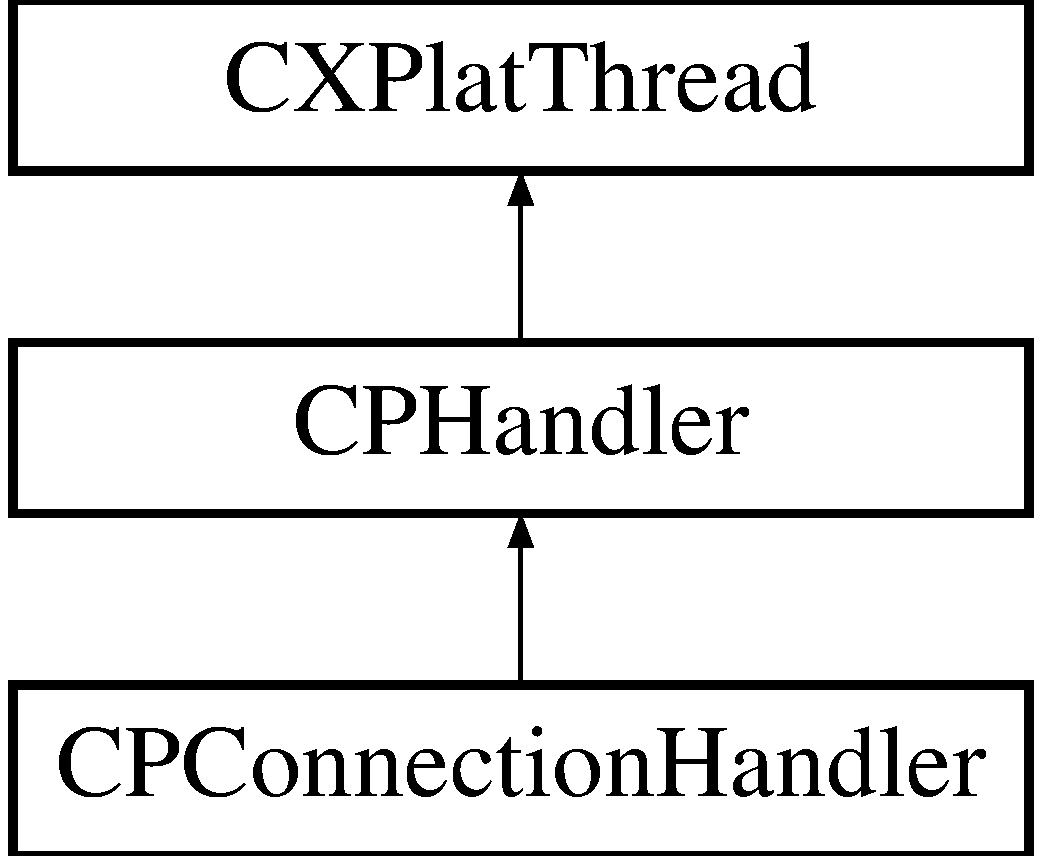
\includegraphics[height=3.000000cm]{class_c_p_connection_handler}
\end{center}
\end{figure}
\subsection*{\-Public \-Member \-Functions}
\begin{DoxyCompactItemize}
\item 
\hyperlink{class_c_p_connection_handler_ad3f9e12330f2741b4e61a457e0980798}{\-C\-P\-Connection\-Handler} (long l\-Close\-Wait\-Milliseconds=0)
\begin{DoxyCompactList}\small\item\em \-Close\-Wait\-Milliseconds is the number of milliseconds after the last send to close the socket. \end{DoxyCompactList}\item 
virtual \hyperlink{class_c_p_connection_handler_a32a850b632fe1f9bd28dec72e1346ad1}{$\sim$\-C\-P\-Connection\-Handler} ()
\end{DoxyCompactItemize}
\subsection*{\-Protected \-Member \-Functions}
\begin{DoxyCompactItemize}
\item 
virtual unsigned \hyperlink{class_c_p_connection_handler_ad7e761b11abc80ceb4573821f38a4244}{\-Worker\-Function} (\hyperlink{_cpclient_8h_a6464f7480a0fd0ee170cba12b2c0497f}{void} $\ast$p\-Param)
\begin{DoxyCompactList}\small\item\em \-Function that does the work. \end{DoxyCompactList}\item 
long \hyperlink{class_c_p_connection_handler_abd4504be00d42202170b8ee762f4f5f3}{\-Get\-Time\-Diff} (long l\-Start, long l\-Finish)
\begin{DoxyCompactList}\small\item\em \-Get \-M\-S difference between 2 times. \end{DoxyCompactList}\end{DoxyCompactItemize}
\subsection*{\-Protected \-Attributes}
\begin{DoxyCompactItemize}
\item 
long \hyperlink{class_c_p_connection_handler_a8d29ca9b1dde7b894038e70a19a9c30f}{l\-Close\-Wait\-M\-S}
\end{DoxyCompactItemize}


\subsection{\-Detailed \-Description}
\hyperlink{class_c_p_connection_handler}{\-C\-P\-Connection\-Handler} does the actual \-I/\-O for each connection. 

\-Definition at line 37 of file \-C\-P\-Connection\-Handler.\-h.



\subsection{\-Constructor \& \-Destructor \-Documentation}
\hypertarget{class_c_p_connection_handler_ad3f9e12330f2741b4e61a457e0980798}{\index{\-C\-P\-Connection\-Handler@{\-C\-P\-Connection\-Handler}!\-C\-P\-Connection\-Handler@{\-C\-P\-Connection\-Handler}}
\index{\-C\-P\-Connection\-Handler@{\-C\-P\-Connection\-Handler}!CPConnectionHandler@{\-C\-P\-Connection\-Handler}}
\subsubsection[{\-C\-P\-Connection\-Handler}]{\setlength{\rightskip}{0pt plus 5cm}{\bf \-C\-P\-Connection\-Handler\-::\-C\-P\-Connection\-Handler} (
\begin{DoxyParamCaption}
\item[{long}]{l\-Close\-Wait\-Milliseconds = {\ttfamily 0}}
\end{DoxyParamCaption}
)}}\label{class_c_p_connection_handler_ad3f9e12330f2741b4e61a457e0980798}


\-Close\-Wait\-Milliseconds is the number of milliseconds after the last send to close the socket. 



\-Definition at line 29 of file \-C\-P\-Connection\-Handler.\-cpp.

\hypertarget{class_c_p_connection_handler_a32a850b632fe1f9bd28dec72e1346ad1}{\index{\-C\-P\-Connection\-Handler@{\-C\-P\-Connection\-Handler}!$\sim$\-C\-P\-Connection\-Handler@{$\sim$\-C\-P\-Connection\-Handler}}
\index{$\sim$\-C\-P\-Connection\-Handler@{$\sim$\-C\-P\-Connection\-Handler}!CPConnectionHandler@{\-C\-P\-Connection\-Handler}}
\subsubsection[{$\sim$\-C\-P\-Connection\-Handler}]{\setlength{\rightskip}{0pt plus 5cm}{\bf \-C\-P\-Connection\-Handler\-::$\sim$\-C\-P\-Connection\-Handler} (
\begin{DoxyParamCaption}
{}
\end{DoxyParamCaption}
)\hspace{0.3cm}{\ttfamily  \mbox{[}virtual\mbox{]}}}}\label{class_c_p_connection_handler_a32a850b632fe1f9bd28dec72e1346ad1}


\-Definition at line 39 of file \-C\-P\-Connection\-Handler.\-cpp.



\subsection{\-Member \-Function \-Documentation}
\hypertarget{class_c_p_connection_handler_abd4504be00d42202170b8ee762f4f5f3}{\index{\-C\-P\-Connection\-Handler@{\-C\-P\-Connection\-Handler}!\-Get\-Time\-Diff@{\-Get\-Time\-Diff}}
\index{\-Get\-Time\-Diff@{\-Get\-Time\-Diff}!CPConnectionHandler@{\-C\-P\-Connection\-Handler}}
\subsubsection[{\-Get\-Time\-Diff}]{\setlength{\rightskip}{0pt plus 5cm}long {\bf \-C\-P\-Connection\-Handler\-::\-Get\-Time\-Diff} (
\begin{DoxyParamCaption}
\item[{long}]{l\-Start, }
\item[{long}]{l\-Finish}
\end{DoxyParamCaption}
)\hspace{0.3cm}{\ttfamily  \mbox{[}protected\mbox{]}}}}\label{class_c_p_connection_handler_abd4504be00d42202170b8ee762f4f5f3}


\-Get \-M\-S difference between 2 times. 



\-Definition at line 217 of file \-C\-P\-Connection\-Handler.\-cpp.

\hypertarget{class_c_p_connection_handler_ad7e761b11abc80ceb4573821f38a4244}{\index{\-C\-P\-Connection\-Handler@{\-C\-P\-Connection\-Handler}!\-Worker\-Function@{\-Worker\-Function}}
\index{\-Worker\-Function@{\-Worker\-Function}!CPConnectionHandler@{\-C\-P\-Connection\-Handler}}
\subsubsection[{\-Worker\-Function}]{\setlength{\rightskip}{0pt plus 5cm}unsigned {\bf \-C\-P\-Connection\-Handler\-::\-Worker\-Function} (
\begin{DoxyParamCaption}
\item[{{\bf void} $\ast$}]{p\-Param}
\end{DoxyParamCaption}
)\hspace{0.3cm}{\ttfamily  \mbox{[}protected, virtual\mbox{]}}}}\label{class_c_p_connection_handler_ad7e761b11abc80ceb4573821f38a4244}


\-Function that does the work. 



\-Implements \hyperlink{class_c_p_handler_a86df3a9d167e20ae405eec33e384bd9b}{\-C\-P\-Handler}.



\-Definition at line 46 of file \-C\-P\-Connection\-Handler.\-cpp.



\subsection{\-Member \-Data \-Documentation}
\hypertarget{class_c_p_connection_handler_a8d29ca9b1dde7b894038e70a19a9c30f}{\index{\-C\-P\-Connection\-Handler@{\-C\-P\-Connection\-Handler}!l\-Close\-Wait\-M\-S@{l\-Close\-Wait\-M\-S}}
\index{l\-Close\-Wait\-M\-S@{l\-Close\-Wait\-M\-S}!CPConnectionHandler@{\-C\-P\-Connection\-Handler}}
\subsubsection[{l\-Close\-Wait\-M\-S}]{\setlength{\rightskip}{0pt plus 5cm}long {\bf \-C\-P\-Connection\-Handler\-::l\-Close\-Wait\-M\-S}\hspace{0.3cm}{\ttfamily  \mbox{[}protected\mbox{]}}}}\label{class_c_p_connection_handler_a8d29ca9b1dde7b894038e70a19a9c30f}


\-Definition at line 50 of file \-C\-P\-Connection\-Handler.\-h.



\-The documentation for this class was generated from the following files\-:\begin{DoxyCompactItemize}
\item 
common/\hyperlink{_c_p_connection_handler_8h}{\-C\-P\-Connection\-Handler.\-h}\item 
common/\hyperlink{_c_p_connection_handler_8cpp}{\-C\-P\-Connection\-Handler.\-cpp}\end{DoxyCompactItemize}

\hypertarget{class_c_p_handler}{\section{\-C\-P\-Handler \-Class \-Reference}
\label{class_c_p_handler}\index{\-C\-P\-Handler@{\-C\-P\-Handler}}
}


\hyperlink{class_c_p_handler}{\-C\-P\-Handler} handles all the connections in a pool, adding, removing, etc.  




{\ttfamily \#include $<$\-C\-P\-Handler.\-h$>$}

\-Inheritance diagram for \-C\-P\-Handler\-:\begin{figure}[H]
\begin{center}
\leavevmode
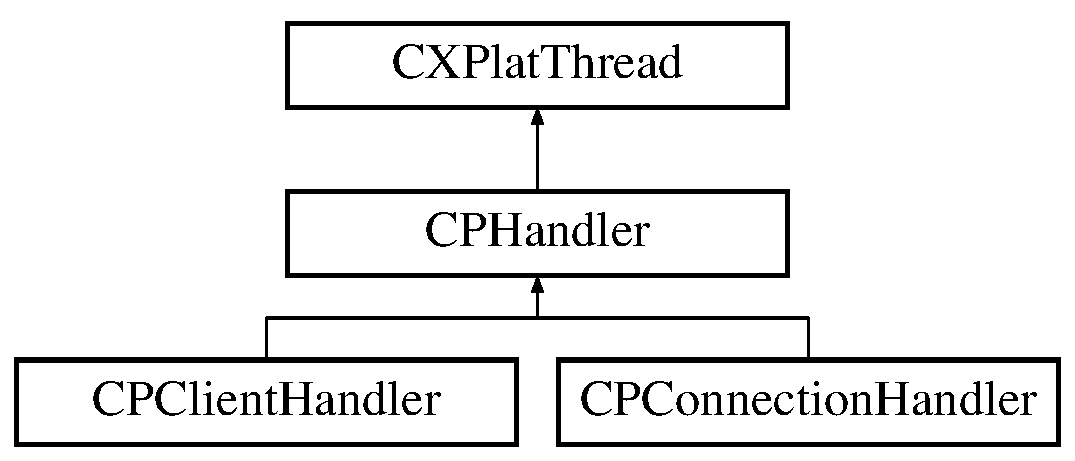
\includegraphics[height=3.000000cm]{class_c_p_handler}
\end{center}
\end{figure}
\subsection*{\-Public \-Member \-Functions}
\begin{DoxyCompactItemize}
\item 
\hyperlink{class_c_p_handler_abc3513acf9f6991bfebf101de8a38895}{\-C\-P\-Handler} ()
\item 
virtual \hyperlink{class_c_p_handler_a83a7da1e9bed8683a9e0e2fa9392f6c0}{$\sim$\-C\-P\-Handler} ()
\item 
virtual \hyperlink{_cpclient_8h_a3be13892ae7076009afcf121347dd319}{\-B\-O\-O\-L} \hyperlink{class_c_p_handler_a0abd34f077a742459ae703aeee7947bc}{\-Add\-Connection} (\hyperlink{class_c_p_connection}{\-C\-P\-Connection} $\ast$p\-Connections, \hyperlink{_x_plat_8h_a8dc8083897335125630f1af5dafd5831}{\-S\-O\-C\-K\-E\-T} \-New\-Socket=\-I\-N\-V\-A\-L\-I\-D\-\_\-\-S\-O\-C\-K\-E\-T)
\begin{DoxyCompactList}\small\item\em \-Add a connection to handle. \end{DoxyCompactList}\item 
virtual \hyperlink{_cpclient_8h_a3be13892ae7076009afcf121347dd319}{\-B\-O\-O\-L} \hyperlink{class_c_p_handler_acd86dd5d6a05124b5c100607aed40bf6}{\-Remove\-Connection} (\hyperlink{class_c_p_connection}{\-C\-P\-Connection} $\ast$p\-Connection)
\begin{DoxyCompactList}\small\item\em \-Remove a connection from our purview. \end{DoxyCompactList}\item 
virtual int \hyperlink{class_c_p_handler_a8f68180d698a456edb91c3e10d8dacc8}{\-Get\-Last\-Size} ()
\begin{DoxyCompactList}\small\item\em \-Get the last size (not necesssarily current) \end{DoxyCompactList}\item 
virtual int \hyperlink{class_c_p_handler_a1610a41117b27ab2805e245eee1a28b1}{\-Get\-Current\-Size} ()
\begin{DoxyCompactList}\small\item\em \-Get the current size (will wait for critical seection) \end{DoxyCompactList}\item 
virtual int \hyperlink{class_c_p_handler_abe1898023c829d3af4b5d1c4efa89479}{\-Call\-Handle\-Connection} (\hyperlink{class_c_p_connection}{\-C\-P\-Connection} $\ast$p\-Connection)
\end{DoxyCompactItemize}
\subsection*{\-Protected \-Member \-Functions}
\begin{DoxyCompactItemize}
\item 
virtual unsigned \hyperlink{class_c_p_handler_a86df3a9d167e20ae405eec33e384bd9b}{\-Worker\-Function} (\hyperlink{_cpclient_8h_a6464f7480a0fd0ee170cba12b2c0497f}{void} $\ast$p\-Param)=0
\begin{DoxyCompactList}\small\item\em \-Function that does the work. \end{DoxyCompactList}\item 
virtual \hyperlink{_cpclient_8h_a6464f7480a0fd0ee170cba12b2c0497f}{void} \hyperlink{class_c_p_handler_a439e2cfd01babb8ba9464a4300e90efe}{\-Call\-Disconnected} (\hyperlink{class_c_p_connection}{\-C\-P\-Connection} $\ast$p\-Connection)
\begin{DoxyCompactList}\small\item\em \-If we want to call the sockets \-Disconnected member. \end{DoxyCompactList}\item 
virtual \hyperlink{_cpclient_8h_a6464f7480a0fd0ee170cba12b2c0497f}{void} \hyperlink{class_c_p_handler_aaa931abc001648da48c2ff82e7071c50}{\-Disconnect\-All} ()
\begin{DoxyCompactList}\small\item\em \-Called in the case of an unrecoverable error. \end{DoxyCompactList}\end{DoxyCompactItemize}
\subsection*{\-Protected \-Attributes}
\begin{DoxyCompactItemize}
\item 
\hyperlink{class_c_x_plat_critical_section}{\-C\-X\-Plat\-Critical\-Section} \hyperlink{class_c_p_handler_a58ba2190209441a5fd44cd4bd1605d79}{c\-Crit\-Map}
\begin{DoxyCompactList}\small\item\em \-To protect c\-Live\-Connections. \end{DoxyCompactList}\item 
\hyperlink{_c_p_handler_8h_ae505ccb84a814fad400e0daede272812}{\-C\-O\-N\-N\-E\-C\-T\-I\-O\-N\-\_\-\-M\-A\-P} \hyperlink{class_c_p_handler_a7ca8fa5c60e6aad56b2b1a2cac68a2e2}{c\-Live\-Connections}
\begin{DoxyCompactList}\small\item\em \-Active connections. \end{DoxyCompactList}\item 
\hyperlink{class_c_x_plat_critical_section}{\-C\-X\-Plat\-Critical\-Section} \hyperlink{class_c_p_handler_a7ffaac647fdd73d143c342bbb88cd379}{c\-Crit\-Queued\-Map}
\begin{DoxyCompactList}\small\item\em \-To protect c\-Queued\-Connections. \end{DoxyCompactList}\item 
\hyperlink{_c_p_handler_8h_ae505ccb84a814fad400e0daede272812}{\-C\-O\-N\-N\-E\-C\-T\-I\-O\-N\-\_\-\-M\-A\-P} \hyperlink{class_c_p_handler_acf71b63ae0b5079e1f8e37cba56f27ea}{c\-Queued\-Connections}
\begin{DoxyCompactList}\small\item\em \-Will add to c\-Live\-Connections at beginning of each \-I/\-O cycle. \end{DoxyCompactList}\item 
int \hyperlink{class_c_p_handler_a23f12318d15c18c8d921efdc80626da4}{i\-Live\-Size}
\begin{DoxyCompactList}\small\item\em \# in c\-Live\-Connections \end{DoxyCompactList}\item 
int \hyperlink{class_c_p_handler_acc98aa0cf09e8d132f239b131a5773da}{i\-Size}
\begin{DoxyCompactList}\small\item\em \# in c\-Live\-Connections + c\-Queued\-Connections \end{DoxyCompactList}\item 
\hyperlink{_cpclient_8h_a3be13892ae7076009afcf121347dd319}{\-B\-O\-O\-L} \hyperlink{class_c_p_handler_a64ec292c01647331e6303ebf6e466d75}{b\-Thread\-Running}
\begin{DoxyCompactList}\small\item\em \-Faster than querying the thread. \end{DoxyCompactList}\end{DoxyCompactItemize}


\subsection{\-Detailed \-Description}
\hyperlink{class_c_p_handler}{\-C\-P\-Handler} handles all the connections in a pool, adding, removing, etc. 

\-Definition at line 35 of file \-C\-P\-Handler.\-h.



\subsection{\-Constructor \& \-Destructor \-Documentation}
\hypertarget{class_c_p_handler_abc3513acf9f6991bfebf101de8a38895}{\index{\-C\-P\-Handler@{\-C\-P\-Handler}!\-C\-P\-Handler@{\-C\-P\-Handler}}
\index{\-C\-P\-Handler@{\-C\-P\-Handler}!CPHandler@{\-C\-P\-Handler}}
\subsubsection[{\-C\-P\-Handler}]{\setlength{\rightskip}{0pt plus 5cm}{\bf \-C\-P\-Handler\-::\-C\-P\-Handler} (
\begin{DoxyParamCaption}
{}
\end{DoxyParamCaption}
)}}\label{class_c_p_handler_abc3513acf9f6991bfebf101de8a38895}


\-Definition at line 28 of file \-C\-P\-Handler.\-cpp.

\hypertarget{class_c_p_handler_a83a7da1e9bed8683a9e0e2fa9392f6c0}{\index{\-C\-P\-Handler@{\-C\-P\-Handler}!$\sim$\-C\-P\-Handler@{$\sim$\-C\-P\-Handler}}
\index{$\sim$\-C\-P\-Handler@{$\sim$\-C\-P\-Handler}!CPHandler@{\-C\-P\-Handler}}
\subsubsection[{$\sim$\-C\-P\-Handler}]{\setlength{\rightskip}{0pt plus 5cm}{\bf \-C\-P\-Handler\-::$\sim$\-C\-P\-Handler} (
\begin{DoxyParamCaption}
{}
\end{DoxyParamCaption}
)\hspace{0.3cm}{\ttfamily  \mbox{[}virtual\mbox{]}}}}\label{class_c_p_handler_a83a7da1e9bed8683a9e0e2fa9392f6c0}


\-Definition at line 38 of file \-C\-P\-Handler.\-cpp.



\subsection{\-Member \-Function \-Documentation}
\hypertarget{class_c_p_handler_a0abd34f077a742459ae703aeee7947bc}{\index{\-C\-P\-Handler@{\-C\-P\-Handler}!\-Add\-Connection@{\-Add\-Connection}}
\index{\-Add\-Connection@{\-Add\-Connection}!CPHandler@{\-C\-P\-Handler}}
\subsubsection[{\-Add\-Connection}]{\setlength{\rightskip}{0pt plus 5cm}{\bf \-B\-O\-O\-L} {\bf \-C\-P\-Handler\-::\-Add\-Connection} (
\begin{DoxyParamCaption}
\item[{{\bf \-C\-P\-Connection} $\ast$}]{p\-Connections, }
\item[{{\bf \-S\-O\-C\-K\-E\-T}}]{\-New\-Socket = {\ttfamily \-I\-N\-V\-A\-L\-I\-D\-\_\-\-S\-O\-C\-K\-E\-T}}
\end{DoxyParamCaption}
)\hspace{0.3cm}{\ttfamily  \mbox{[}virtual\mbox{]}}}}\label{class_c_p_handler_a0abd34f077a742459ae703aeee7947bc}


\-Add a connection to handle. 



\-Definition at line 48 of file \-C\-P\-Handler.\-cpp.

\hypertarget{class_c_p_handler_a439e2cfd01babb8ba9464a4300e90efe}{\index{\-C\-P\-Handler@{\-C\-P\-Handler}!\-Call\-Disconnected@{\-Call\-Disconnected}}
\index{\-Call\-Disconnected@{\-Call\-Disconnected}!CPHandler@{\-C\-P\-Handler}}
\subsubsection[{\-Call\-Disconnected}]{\setlength{\rightskip}{0pt plus 5cm}{\bf void} {\bf \-C\-P\-Handler\-::\-Call\-Disconnected} (
\begin{DoxyParamCaption}
\item[{{\bf \-C\-P\-Connection} $\ast$}]{p\-Connection}
\end{DoxyParamCaption}
)\hspace{0.3cm}{\ttfamily  \mbox{[}protected, virtual\mbox{]}}}}\label{class_c_p_handler_a439e2cfd01babb8ba9464a4300e90efe}


\-If we want to call the sockets \-Disconnected member. 



\-Reimplemented in \hyperlink{class_c_p_client_handler_ad6df6ba23365c140780ddd27cb44bd08}{\-C\-P\-Client\-Handler}.



\-Definition at line 208 of file \-C\-P\-Handler.\-cpp.

\hypertarget{class_c_p_handler_abe1898023c829d3af4b5d1c4efa89479}{\index{\-C\-P\-Handler@{\-C\-P\-Handler}!\-Call\-Handle\-Connection@{\-Call\-Handle\-Connection}}
\index{\-Call\-Handle\-Connection@{\-Call\-Handle\-Connection}!CPHandler@{\-C\-P\-Handler}}
\subsubsection[{\-Call\-Handle\-Connection}]{\setlength{\rightskip}{0pt plus 5cm}int {\bf \-C\-P\-Handler\-::\-Call\-Handle\-Connection} (
\begin{DoxyParamCaption}
\item[{{\bf \-C\-P\-Connection} $\ast$}]{p\-Connection}
\end{DoxyParamCaption}
)\hspace{0.3cm}{\ttfamily  \mbox{[}virtual\mbox{]}}}}\label{class_c_p_handler_abe1898023c829d3af4b5d1c4efa89479}
\-Call the \-C\-P\-Connection-\/$>$\-Handle\-Connection \-This is here so derived classes can choose \-N\-O\-T to call it in case the handler is chained (like the \hyperlink{class_c_p_client_handler}{\-C\-P\-Client\-Handler}) 

\-Reimplemented in \hyperlink{class_c_p_client_handler_a7f6d153c5104840663b7225a36ea7609}{\-C\-P\-Client\-Handler}.



\-Definition at line 198 of file \-C\-P\-Handler.\-cpp.

\hypertarget{class_c_p_handler_aaa931abc001648da48c2ff82e7071c50}{\index{\-C\-P\-Handler@{\-C\-P\-Handler}!\-Disconnect\-All@{\-Disconnect\-All}}
\index{\-Disconnect\-All@{\-Disconnect\-All}!CPHandler@{\-C\-P\-Handler}}
\subsubsection[{\-Disconnect\-All}]{\setlength{\rightskip}{0pt plus 5cm}{\bf void} {\bf \-C\-P\-Handler\-::\-Disconnect\-All} (
\begin{DoxyParamCaption}
{}
\end{DoxyParamCaption}
)\hspace{0.3cm}{\ttfamily  \mbox{[}protected, virtual\mbox{]}}}}\label{class_c_p_handler_aaa931abc001648da48c2ff82e7071c50}


\-Called in the case of an unrecoverable error. 



\-Definition at line 162 of file \-C\-P\-Handler.\-cpp.

\hypertarget{class_c_p_handler_a1610a41117b27ab2805e245eee1a28b1}{\index{\-C\-P\-Handler@{\-C\-P\-Handler}!\-Get\-Current\-Size@{\-Get\-Current\-Size}}
\index{\-Get\-Current\-Size@{\-Get\-Current\-Size}!CPHandler@{\-C\-P\-Handler}}
\subsubsection[{\-Get\-Current\-Size}]{\setlength{\rightskip}{0pt plus 5cm}int {\bf \-C\-P\-Handler\-::\-Get\-Current\-Size} (
\begin{DoxyParamCaption}
{}
\end{DoxyParamCaption}
)\hspace{0.3cm}{\ttfamily  \mbox{[}virtual\mbox{]}}}}\label{class_c_p_handler_a1610a41117b27ab2805e245eee1a28b1}


\-Get the current size (will wait for critical seection) 



\-Definition at line 189 of file \-C\-P\-Handler.\-cpp.

\hypertarget{class_c_p_handler_a8f68180d698a456edb91c3e10d8dacc8}{\index{\-C\-P\-Handler@{\-C\-P\-Handler}!\-Get\-Last\-Size@{\-Get\-Last\-Size}}
\index{\-Get\-Last\-Size@{\-Get\-Last\-Size}!CPHandler@{\-C\-P\-Handler}}
\subsubsection[{\-Get\-Last\-Size}]{\setlength{\rightskip}{0pt plus 5cm}int {\bf \-C\-P\-Handler\-::\-Get\-Last\-Size} (
\begin{DoxyParamCaption}
{}
\end{DoxyParamCaption}
)\hspace{0.3cm}{\ttfamily  \mbox{[}virtual\mbox{]}}}}\label{class_c_p_handler_a8f68180d698a456edb91c3e10d8dacc8}


\-Get the last size (not necesssarily current) 



\-Definition at line 182 of file \-C\-P\-Handler.\-cpp.

\hypertarget{class_c_p_handler_acd86dd5d6a05124b5c100607aed40bf6}{\index{\-C\-P\-Handler@{\-C\-P\-Handler}!\-Remove\-Connection@{\-Remove\-Connection}}
\index{\-Remove\-Connection@{\-Remove\-Connection}!CPHandler@{\-C\-P\-Handler}}
\subsubsection[{\-Remove\-Connection}]{\setlength{\rightskip}{0pt plus 5cm}{\bf \-B\-O\-O\-L} {\bf \-C\-P\-Handler\-::\-Remove\-Connection} (
\begin{DoxyParamCaption}
\item[{{\bf \-C\-P\-Connection} $\ast$}]{p\-Connection}
\end{DoxyParamCaption}
)\hspace{0.3cm}{\ttfamily  \mbox{[}virtual\mbox{]}}}}\label{class_c_p_handler_acd86dd5d6a05124b5c100607aed40bf6}


\-Remove a connection from our purview. 



\-Definition at line 105 of file \-C\-P\-Handler.\-cpp.

\hypertarget{class_c_p_handler_a86df3a9d167e20ae405eec33e384bd9b}{\index{\-C\-P\-Handler@{\-C\-P\-Handler}!\-Worker\-Function@{\-Worker\-Function}}
\index{\-Worker\-Function@{\-Worker\-Function}!CPHandler@{\-C\-P\-Handler}}
\subsubsection[{\-Worker\-Function}]{\setlength{\rightskip}{0pt plus 5cm}virtual unsigned {\bf \-C\-P\-Handler\-::\-Worker\-Function} (
\begin{DoxyParamCaption}
\item[{{\bf void} $\ast$}]{p\-Param}
\end{DoxyParamCaption}
)\hspace{0.3cm}{\ttfamily  \mbox{[}protected, pure virtual\mbox{]}}}}\label{class_c_p_handler_a86df3a9d167e20ae405eec33e384bd9b}


\-Function that does the work. 



\-Implements \hyperlink{class_c_x_plat_thread_af8a15900817f9673c6fd8e85cdedf27d}{\-C\-X\-Plat\-Thread}.



\-Implemented in \hyperlink{class_c_p_client_handler_a88117dfe5e1e6d2f5d953277bc1a3044}{\-C\-P\-Client\-Handler}, and \hyperlink{class_c_p_connection_handler_ad7e761b11abc80ceb4573821f38a4244}{\-C\-P\-Connection\-Handler}.



\subsection{\-Member \-Data \-Documentation}
\hypertarget{class_c_p_handler_a64ec292c01647331e6303ebf6e466d75}{\index{\-C\-P\-Handler@{\-C\-P\-Handler}!b\-Thread\-Running@{b\-Thread\-Running}}
\index{b\-Thread\-Running@{b\-Thread\-Running}!CPHandler@{\-C\-P\-Handler}}
\subsubsection[{b\-Thread\-Running}]{\setlength{\rightskip}{0pt plus 5cm}{\bf \-B\-O\-O\-L} {\bf \-C\-P\-Handler\-::b\-Thread\-Running}\hspace{0.3cm}{\ttfamily  \mbox{[}protected\mbox{]}}}}\label{class_c_p_handler_a64ec292c01647331e6303ebf6e466d75}


\-Faster than querying the thread. 



\-Definition at line 75 of file \-C\-P\-Handler.\-h.

\hypertarget{class_c_p_handler_a58ba2190209441a5fd44cd4bd1605d79}{\index{\-C\-P\-Handler@{\-C\-P\-Handler}!c\-Crit\-Map@{c\-Crit\-Map}}
\index{c\-Crit\-Map@{c\-Crit\-Map}!CPHandler@{\-C\-P\-Handler}}
\subsubsection[{c\-Crit\-Map}]{\setlength{\rightskip}{0pt plus 5cm}{\bf \-C\-X\-Plat\-Critical\-Section} {\bf \-C\-P\-Handler\-::c\-Crit\-Map}\hspace{0.3cm}{\ttfamily  \mbox{[}protected\mbox{]}}}}\label{class_c_p_handler_a58ba2190209441a5fd44cd4bd1605d79}


\-To protect c\-Live\-Connections. 



\-Definition at line 63 of file \-C\-P\-Handler.\-h.

\hypertarget{class_c_p_handler_a7ffaac647fdd73d143c342bbb88cd379}{\index{\-C\-P\-Handler@{\-C\-P\-Handler}!c\-Crit\-Queued\-Map@{c\-Crit\-Queued\-Map}}
\index{c\-Crit\-Queued\-Map@{c\-Crit\-Queued\-Map}!CPHandler@{\-C\-P\-Handler}}
\subsubsection[{c\-Crit\-Queued\-Map}]{\setlength{\rightskip}{0pt plus 5cm}{\bf \-C\-X\-Plat\-Critical\-Section} {\bf \-C\-P\-Handler\-::c\-Crit\-Queued\-Map}\hspace{0.3cm}{\ttfamily  \mbox{[}protected\mbox{]}}}}\label{class_c_p_handler_a7ffaac647fdd73d143c342bbb88cd379}


\-To protect c\-Queued\-Connections. 



\-Definition at line 67 of file \-C\-P\-Handler.\-h.

\hypertarget{class_c_p_handler_a7ca8fa5c60e6aad56b2b1a2cac68a2e2}{\index{\-C\-P\-Handler@{\-C\-P\-Handler}!c\-Live\-Connections@{c\-Live\-Connections}}
\index{c\-Live\-Connections@{c\-Live\-Connections}!CPHandler@{\-C\-P\-Handler}}
\subsubsection[{c\-Live\-Connections}]{\setlength{\rightskip}{0pt plus 5cm}{\bf \-C\-O\-N\-N\-E\-C\-T\-I\-O\-N\-\_\-\-M\-A\-P} {\bf \-C\-P\-Handler\-::c\-Live\-Connections}\hspace{0.3cm}{\ttfamily  \mbox{[}protected\mbox{]}}}}\label{class_c_p_handler_a7ca8fa5c60e6aad56b2b1a2cac68a2e2}


\-Active connections. 



\-Definition at line 65 of file \-C\-P\-Handler.\-h.

\hypertarget{class_c_p_handler_acf71b63ae0b5079e1f8e37cba56f27ea}{\index{\-C\-P\-Handler@{\-C\-P\-Handler}!c\-Queued\-Connections@{c\-Queued\-Connections}}
\index{c\-Queued\-Connections@{c\-Queued\-Connections}!CPHandler@{\-C\-P\-Handler}}
\subsubsection[{c\-Queued\-Connections}]{\setlength{\rightskip}{0pt plus 5cm}{\bf \-C\-O\-N\-N\-E\-C\-T\-I\-O\-N\-\_\-\-M\-A\-P} {\bf \-C\-P\-Handler\-::c\-Queued\-Connections}\hspace{0.3cm}{\ttfamily  \mbox{[}protected\mbox{]}}}}\label{class_c_p_handler_acf71b63ae0b5079e1f8e37cba56f27ea}


\-Will add to c\-Live\-Connections at beginning of each \-I/\-O cycle. 



\-Definition at line 69 of file \-C\-P\-Handler.\-h.

\hypertarget{class_c_p_handler_a23f12318d15c18c8d921efdc80626da4}{\index{\-C\-P\-Handler@{\-C\-P\-Handler}!i\-Live\-Size@{i\-Live\-Size}}
\index{i\-Live\-Size@{i\-Live\-Size}!CPHandler@{\-C\-P\-Handler}}
\subsubsection[{i\-Live\-Size}]{\setlength{\rightskip}{0pt plus 5cm}int {\bf \-C\-P\-Handler\-::i\-Live\-Size}\hspace{0.3cm}{\ttfamily  \mbox{[}protected\mbox{]}}}}\label{class_c_p_handler_a23f12318d15c18c8d921efdc80626da4}


\# in c\-Live\-Connections 



\-Definition at line 71 of file \-C\-P\-Handler.\-h.

\hypertarget{class_c_p_handler_acc98aa0cf09e8d132f239b131a5773da}{\index{\-C\-P\-Handler@{\-C\-P\-Handler}!i\-Size@{i\-Size}}
\index{i\-Size@{i\-Size}!CPHandler@{\-C\-P\-Handler}}
\subsubsection[{i\-Size}]{\setlength{\rightskip}{0pt plus 5cm}int {\bf \-C\-P\-Handler\-::i\-Size}\hspace{0.3cm}{\ttfamily  \mbox{[}protected\mbox{]}}}}\label{class_c_p_handler_acc98aa0cf09e8d132f239b131a5773da}


\# in c\-Live\-Connections + c\-Queued\-Connections 



\-Definition at line 73 of file \-C\-P\-Handler.\-h.



\-The documentation for this class was generated from the following files\-:\begin{DoxyCompactItemize}
\item 
common/\hyperlink{_c_p_handler_8h}{\-C\-P\-Handler.\-h}\item 
common/\hyperlink{_c_p_handler_8cpp}{\-C\-P\-Handler.\-cpp}\end{DoxyCompactItemize}

\hypertarget{class_c_profile_timer}{\section{\-C\-Profile\-Timer \-Class \-Reference}
\label{class_c_profile_timer}\index{\-C\-Profile\-Timer@{\-C\-Profile\-Timer}}
}


{\ttfamily \#include $<$\-C\-Profile\-Timer.\-h$>$}

\subsection*{\-Public \-Member \-Functions}
\begin{DoxyCompactItemize}
\item 
\hyperlink{class_c_profile_timer_a92dc183d7ad6024bbef9ddf7c11575e3}{\-C\-Profile\-Timer} ()
\item 
virtual \hyperlink{class_c_profile_timer_a509d0492413e3f19975744b9146cbf4f}{$\sim$\-C\-Profile\-Timer} ()
\item 
\hyperlink{_cpclient_8h_a6464f7480a0fd0ee170cba12b2c0497f}{void} \hyperlink{class_c_profile_timer_a8ca922af73784e9a805b3fc91d99328e}{\-Start} ()
\item 
\hyperlink{_cpclient_8h_a6464f7480a0fd0ee170cba12b2c0497f}{void} \hyperlink{class_c_profile_timer_ab2e930ba032083e6276940236bc78551}{\-Get\-Elapsed\-Time} (\hyperlink{class_elapsed_time}{\-Elapsed\-Time} \&c\-Elapsed, bool b\-Reset=true)
\end{DoxyCompactItemize}
\subsection*{\-Static \-Public \-Member \-Functions}
\begin{DoxyCompactItemize}
\item 
static \hyperlink{_cpclient_8h_a6464f7480a0fd0ee170cba12b2c0497f}{void} \hyperlink{class_c_profile_timer_a46d890dae6ed61d728fecde8a68ead61}{\-Set\-Timestamp} (const char $\ast$p\-Label)
\item 
static \hyperlink{_cpclient_8h_a6464f7480a0fd0ee170cba12b2c0497f}{void} \hyperlink{class_c_profile_timer_a45d63f2f6b9a92a5e7069cef9a402d38}{\-Get\-Elapsed} (\hyperlink{class_elapsed_time}{\-Elapsed\-Time} \&c\-Elapsed, const char $\ast$p\-Label1, const char $\ast$p\-Label2, bool b\-Mark\-Label2=false)
\item 
static \hyperlink{_cpclient_8h_a6464f7480a0fd0ee170cba12b2c0497f}{void} \hyperlink{class_c_profile_timer_a2a4035c04b45fbb802d09fd4643fd6b5}{\-Get\-Elapsed\-Now} (\hyperlink{class_elapsed_time}{\-Elapsed\-Time} \&c\-Elapsed, const char $\ast$p\-Label1)
\item 
static \hyperlink{_cpclient_8h_a6464f7480a0fd0ee170cba12b2c0497f}{void} \hyperlink{class_c_profile_timer_a79631bee05a1a67ed38bcaf32c24da7a}{\-Print\-Elapsed} (const char $\ast$p\-Label1, const char $\ast$p\-Label2, bool b\-Mark\-Label2=false, const char $\ast$p\-Tag=\-N\-U\-L\-L)
\item 
static long \hyperlink{class_c_profile_timer_a8375a594f2842375b5c53755c1c0ce1d}{\-Get\-Elapsed\-M\-S} (const char $\ast$p\-Label1, const char $\ast$p\-Label2, bool b\-Mark\-Label2=false)
\item 
static \hyperlink{_cpclient_8h_a6464f7480a0fd0ee170cba12b2c0497f}{void} \hyperlink{class_c_profile_timer_ae4f2f0a7f4b60a7fbf1316da4021c59b}{\-Clear} ()
\end{DoxyCompactItemize}
\subsection*{\-Static \-Protected \-Member \-Functions}
\begin{DoxyCompactItemize}
\item 
static struct timeval \hyperlink{class_c_profile_timer_a4d38b3a9eaa88823dadb431760140569}{\-Get\-Label\-Timestamp} (const char $\ast$p\-Label)
\item 
static \hyperlink{class_elapsed_time}{\-Elapsed\-Time} \hyperlink{class_c_profile_timer_a89f47c18a0f65740fcb6939646b99978}{\-Get\-Difference} (\hyperlink{class_elapsed_time}{\-Elapsed\-Time} \&c\-Elapsed, struct timeval $\ast$s\-T1, struct timeval $\ast$s\-T2)
\end{DoxyCompactItemize}
\subsection*{\-Protected \-Attributes}
\begin{DoxyCompactItemize}
\item 
struct timeval \hyperlink{class_c_profile_timer_a4c80bee9e1f0f119a091f46888507b99}{s\-Start}
\item 
struct timeval \hyperlink{class_c_profile_timer_ac51e8e2333d5c218d86414a25d55f224}{s\-End}
\end{DoxyCompactItemize}


\subsection{\-Detailed \-Description}


\-Definition at line 61 of file \-C\-Profile\-Timer.\-h.



\subsection{\-Constructor \& \-Destructor \-Documentation}
\hypertarget{class_c_profile_timer_a92dc183d7ad6024bbef9ddf7c11575e3}{\index{\-C\-Profile\-Timer@{\-C\-Profile\-Timer}!\-C\-Profile\-Timer@{\-C\-Profile\-Timer}}
\index{\-C\-Profile\-Timer@{\-C\-Profile\-Timer}!CProfileTimer@{\-C\-Profile\-Timer}}
\subsubsection[{\-C\-Profile\-Timer}]{\setlength{\rightskip}{0pt plus 5cm}{\bf \-C\-Profile\-Timer\-::\-C\-Profile\-Timer} (
\begin{DoxyParamCaption}
{}
\end{DoxyParamCaption}
)}}\label{class_c_profile_timer_a92dc183d7ad6024bbef9ddf7c11575e3}


\-Definition at line 28 of file \-C\-Profile\-Timer.\-cpp.

\hypertarget{class_c_profile_timer_a509d0492413e3f19975744b9146cbf4f}{\index{\-C\-Profile\-Timer@{\-C\-Profile\-Timer}!$\sim$\-C\-Profile\-Timer@{$\sim$\-C\-Profile\-Timer}}
\index{$\sim$\-C\-Profile\-Timer@{$\sim$\-C\-Profile\-Timer}!CProfileTimer@{\-C\-Profile\-Timer}}
\subsubsection[{$\sim$\-C\-Profile\-Timer}]{\setlength{\rightskip}{0pt plus 5cm}{\bf \-C\-Profile\-Timer\-::$\sim$\-C\-Profile\-Timer} (
\begin{DoxyParamCaption}
{}
\end{DoxyParamCaption}
)\hspace{0.3cm}{\ttfamily  \mbox{[}virtual\mbox{]}}}}\label{class_c_profile_timer_a509d0492413e3f19975744b9146cbf4f}


\-Definition at line 33 of file \-C\-Profile\-Timer.\-cpp.



\subsection{\-Member \-Function \-Documentation}
\hypertarget{class_c_profile_timer_ae4f2f0a7f4b60a7fbf1316da4021c59b}{\index{\-C\-Profile\-Timer@{\-C\-Profile\-Timer}!\-Clear@{\-Clear}}
\index{\-Clear@{\-Clear}!CProfileTimer@{\-C\-Profile\-Timer}}
\subsubsection[{\-Clear}]{\setlength{\rightskip}{0pt plus 5cm}{\bf void} {\bf \-C\-Profile\-Timer\-::\-Clear} (
\begin{DoxyParamCaption}
{}
\end{DoxyParamCaption}
)\hspace{0.3cm}{\ttfamily  \mbox{[}static\mbox{]}}}}\label{class_c_profile_timer_ae4f2f0a7f4b60a7fbf1316da4021c59b}


\-Definition at line 186 of file \-C\-Profile\-Timer.\-cpp.

\hypertarget{class_c_profile_timer_a89f47c18a0f65740fcb6939646b99978}{\index{\-C\-Profile\-Timer@{\-C\-Profile\-Timer}!\-Get\-Difference@{\-Get\-Difference}}
\index{\-Get\-Difference@{\-Get\-Difference}!CProfileTimer@{\-C\-Profile\-Timer}}
\subsubsection[{\-Get\-Difference}]{\setlength{\rightskip}{0pt plus 5cm}{\bf \-Elapsed\-Time} {\bf \-C\-Profile\-Timer\-::\-Get\-Difference} (
\begin{DoxyParamCaption}
\item[{{\bf \-Elapsed\-Time} \&}]{c\-Elapsed, }
\item[{struct timeval $\ast$}]{s\-T1, }
\item[{struct timeval $\ast$}]{s\-T2}
\end{DoxyParamCaption}
)\hspace{0.3cm}{\ttfamily  \mbox{[}static, protected\mbox{]}}}}\label{class_c_profile_timer_a89f47c18a0f65740fcb6939646b99978}


\-Definition at line 91 of file \-C\-Profile\-Timer.\-cpp.

\hypertarget{class_c_profile_timer_a45d63f2f6b9a92a5e7069cef9a402d38}{\index{\-C\-Profile\-Timer@{\-C\-Profile\-Timer}!\-Get\-Elapsed@{\-Get\-Elapsed}}
\index{\-Get\-Elapsed@{\-Get\-Elapsed}!CProfileTimer@{\-C\-Profile\-Timer}}
\subsubsection[{\-Get\-Elapsed}]{\setlength{\rightskip}{0pt plus 5cm}{\bf void} {\bf \-C\-Profile\-Timer\-::\-Get\-Elapsed} (
\begin{DoxyParamCaption}
\item[{{\bf \-Elapsed\-Time} \&}]{c\-Elapsed, }
\item[{const char $\ast$}]{p\-Label1, }
\item[{const char $\ast$}]{p\-Label2, }
\item[{bool}]{b\-Mark\-Label2 = {\ttfamily false}}
\end{DoxyParamCaption}
)\hspace{0.3cm}{\ttfamily  \mbox{[}static\mbox{]}}}}\label{class_c_profile_timer_a45d63f2f6b9a92a5e7069cef9a402d38}


\-Definition at line 116 of file \-C\-Profile\-Timer.\-cpp.

\hypertarget{class_c_profile_timer_a8375a594f2842375b5c53755c1c0ce1d}{\index{\-C\-Profile\-Timer@{\-C\-Profile\-Timer}!\-Get\-Elapsed\-M\-S@{\-Get\-Elapsed\-M\-S}}
\index{\-Get\-Elapsed\-M\-S@{\-Get\-Elapsed\-M\-S}!CProfileTimer@{\-C\-Profile\-Timer}}
\subsubsection[{\-Get\-Elapsed\-M\-S}]{\setlength{\rightskip}{0pt plus 5cm}long {\bf \-C\-Profile\-Timer\-::\-Get\-Elapsed\-M\-S} (
\begin{DoxyParamCaption}
\item[{const char $\ast$}]{p\-Label1, }
\item[{const char $\ast$}]{p\-Label2, }
\item[{bool}]{b\-Mark\-Label2 = {\ttfamily false}}
\end{DoxyParamCaption}
)\hspace{0.3cm}{\ttfamily  \mbox{[}static\mbox{]}}}}\label{class_c_profile_timer_a8375a594f2842375b5c53755c1c0ce1d}


\-Definition at line 175 of file \-C\-Profile\-Timer.\-cpp.

\hypertarget{class_c_profile_timer_a2a4035c04b45fbb802d09fd4643fd6b5}{\index{\-C\-Profile\-Timer@{\-C\-Profile\-Timer}!\-Get\-Elapsed\-Now@{\-Get\-Elapsed\-Now}}
\index{\-Get\-Elapsed\-Now@{\-Get\-Elapsed\-Now}!CProfileTimer@{\-C\-Profile\-Timer}}
\subsubsection[{\-Get\-Elapsed\-Now}]{\setlength{\rightskip}{0pt plus 5cm}{\bf void} {\bf \-C\-Profile\-Timer\-::\-Get\-Elapsed\-Now} (
\begin{DoxyParamCaption}
\item[{{\bf \-Elapsed\-Time} \&}]{c\-Elapsed, }
\item[{const char $\ast$}]{p\-Label1}
\end{DoxyParamCaption}
)\hspace{0.3cm}{\ttfamily  \mbox{[}static\mbox{]}}}}\label{class_c_profile_timer_a2a4035c04b45fbb802d09fd4643fd6b5}


\-Definition at line 136 of file \-C\-Profile\-Timer.\-cpp.

\hypertarget{class_c_profile_timer_ab2e930ba032083e6276940236bc78551}{\index{\-C\-Profile\-Timer@{\-C\-Profile\-Timer}!\-Get\-Elapsed\-Time@{\-Get\-Elapsed\-Time}}
\index{\-Get\-Elapsed\-Time@{\-Get\-Elapsed\-Time}!CProfileTimer@{\-C\-Profile\-Timer}}
\subsubsection[{\-Get\-Elapsed\-Time}]{\setlength{\rightskip}{0pt plus 5cm}{\bf void} {\bf \-C\-Profile\-Timer\-::\-Get\-Elapsed\-Time} (
\begin{DoxyParamCaption}
\item[{{\bf \-Elapsed\-Time} \&}]{c\-Elapsed, }
\item[{bool}]{b\-Reset = {\ttfamily true}}
\end{DoxyParamCaption}
)}}\label{class_c_profile_timer_ab2e930ba032083e6276940236bc78551}


\-Definition at line 79 of file \-C\-Profile\-Timer.\-cpp.

\hypertarget{class_c_profile_timer_a4d38b3a9eaa88823dadb431760140569}{\index{\-C\-Profile\-Timer@{\-C\-Profile\-Timer}!\-Get\-Label\-Timestamp@{\-Get\-Label\-Timestamp}}
\index{\-Get\-Label\-Timestamp@{\-Get\-Label\-Timestamp}!CProfileTimer@{\-C\-Profile\-Timer}}
\subsubsection[{\-Get\-Label\-Timestamp}]{\setlength{\rightskip}{0pt plus 5cm}struct timeval {\bf \-C\-Profile\-Timer\-::\-Get\-Label\-Timestamp} (
\begin{DoxyParamCaption}
\item[{const char $\ast$}]{p\-Label}
\end{DoxyParamCaption}
)\hspace{0.3cm}{\ttfamily  \mbox{[}static, read, protected\mbox{]}}}}\label{class_c_profile_timer_a4d38b3a9eaa88823dadb431760140569}


\-Definition at line 40 of file \-C\-Profile\-Timer.\-cpp.

\hypertarget{class_c_profile_timer_a79631bee05a1a67ed38bcaf32c24da7a}{\index{\-C\-Profile\-Timer@{\-C\-Profile\-Timer}!\-Print\-Elapsed@{\-Print\-Elapsed}}
\index{\-Print\-Elapsed@{\-Print\-Elapsed}!CProfileTimer@{\-C\-Profile\-Timer}}
\subsubsection[{\-Print\-Elapsed}]{\setlength{\rightskip}{0pt plus 5cm}{\bf void} {\bf \-C\-Profile\-Timer\-::\-Print\-Elapsed} (
\begin{DoxyParamCaption}
\item[{const char $\ast$}]{p\-Label1, }
\item[{const char $\ast$}]{p\-Label2, }
\item[{bool}]{b\-Mark\-Label2 = {\ttfamily false}, }
\item[{const char $\ast$}]{p\-Tag = {\ttfamily \-N\-U\-L\-L}}
\end{DoxyParamCaption}
)\hspace{0.3cm}{\ttfamily  \mbox{[}static\mbox{]}}}}\label{class_c_profile_timer_a79631bee05a1a67ed38bcaf32c24da7a}


\-Definition at line 155 of file \-C\-Profile\-Timer.\-cpp.

\hypertarget{class_c_profile_timer_a46d890dae6ed61d728fecde8a68ead61}{\index{\-C\-Profile\-Timer@{\-C\-Profile\-Timer}!\-Set\-Timestamp@{\-Set\-Timestamp}}
\index{\-Set\-Timestamp@{\-Set\-Timestamp}!CProfileTimer@{\-C\-Profile\-Timer}}
\subsubsection[{\-Set\-Timestamp}]{\setlength{\rightskip}{0pt plus 5cm}{\bf void} {\bf \-C\-Profile\-Timer\-::\-Set\-Timestamp} (
\begin{DoxyParamCaption}
\item[{const char $\ast$}]{p\-Label}
\end{DoxyParamCaption}
)\hspace{0.3cm}{\ttfamily  \mbox{[}static\mbox{]}}}}\label{class_c_profile_timer_a46d890dae6ed61d728fecde8a68ead61}


\-Definition at line 58 of file \-C\-Profile\-Timer.\-cpp.

\hypertarget{class_c_profile_timer_a8ca922af73784e9a805b3fc91d99328e}{\index{\-C\-Profile\-Timer@{\-C\-Profile\-Timer}!\-Start@{\-Start}}
\index{\-Start@{\-Start}!CProfileTimer@{\-C\-Profile\-Timer}}
\subsubsection[{\-Start}]{\setlength{\rightskip}{0pt plus 5cm}{\bf void} {\bf \-C\-Profile\-Timer\-::\-Start} (
\begin{DoxyParamCaption}
{}
\end{DoxyParamCaption}
)}}\label{class_c_profile_timer_a8ca922af73784e9a805b3fc91d99328e}


\-Definition at line 73 of file \-C\-Profile\-Timer.\-cpp.



\subsection{\-Member \-Data \-Documentation}
\hypertarget{class_c_profile_timer_ac51e8e2333d5c218d86414a25d55f224}{\index{\-C\-Profile\-Timer@{\-C\-Profile\-Timer}!s\-End@{s\-End}}
\index{s\-End@{s\-End}!CProfileTimer@{\-C\-Profile\-Timer}}
\subsubsection[{s\-End}]{\setlength{\rightskip}{0pt plus 5cm}struct timeval {\bf \-C\-Profile\-Timer\-::s\-End}\hspace{0.3cm}{\ttfamily  \mbox{[}protected\mbox{]}}}}\label{class_c_profile_timer_ac51e8e2333d5c218d86414a25d55f224}


\-Definition at line 90 of file \-C\-Profile\-Timer.\-h.

\hypertarget{class_c_profile_timer_a4c80bee9e1f0f119a091f46888507b99}{\index{\-C\-Profile\-Timer@{\-C\-Profile\-Timer}!s\-Start@{s\-Start}}
\index{s\-Start@{s\-Start}!CProfileTimer@{\-C\-Profile\-Timer}}
\subsubsection[{s\-Start}]{\setlength{\rightskip}{0pt plus 5cm}struct timeval {\bf \-C\-Profile\-Timer\-::s\-Start}\hspace{0.3cm}{\ttfamily  \mbox{[}protected\mbox{]}}}}\label{class_c_profile_timer_a4c80bee9e1f0f119a091f46888507b99}


\-Definition at line 89 of file \-C\-Profile\-Timer.\-h.



\-The documentation for this class was generated from the following files\-:\begin{DoxyCompactItemize}
\item 
common/\hyperlink{_c_profile_timer_8h}{\-C\-Profile\-Timer.\-h}\item 
common/\hyperlink{_c_profile_timer_8cpp}{\-C\-Profile\-Timer.\-cpp}\end{DoxyCompactItemize}

\hypertarget{class_c_p_server}{\section{\-C\-P\-Server \-Class \-Reference}
\label{class_c_p_server}\index{\-C\-P\-Server@{\-C\-P\-Server}}
}


\-C\-P\-Server.\-h\-: interface for the \hyperlink{class_c_p_server}{\-C\-P\-Server} class.  




{\ttfamily \#include $<$\-Cpserver.\-h$>$}

\-Inheritance diagram for \-C\-P\-Server\-:\begin{figure}[H]
\begin{center}
\leavevmode
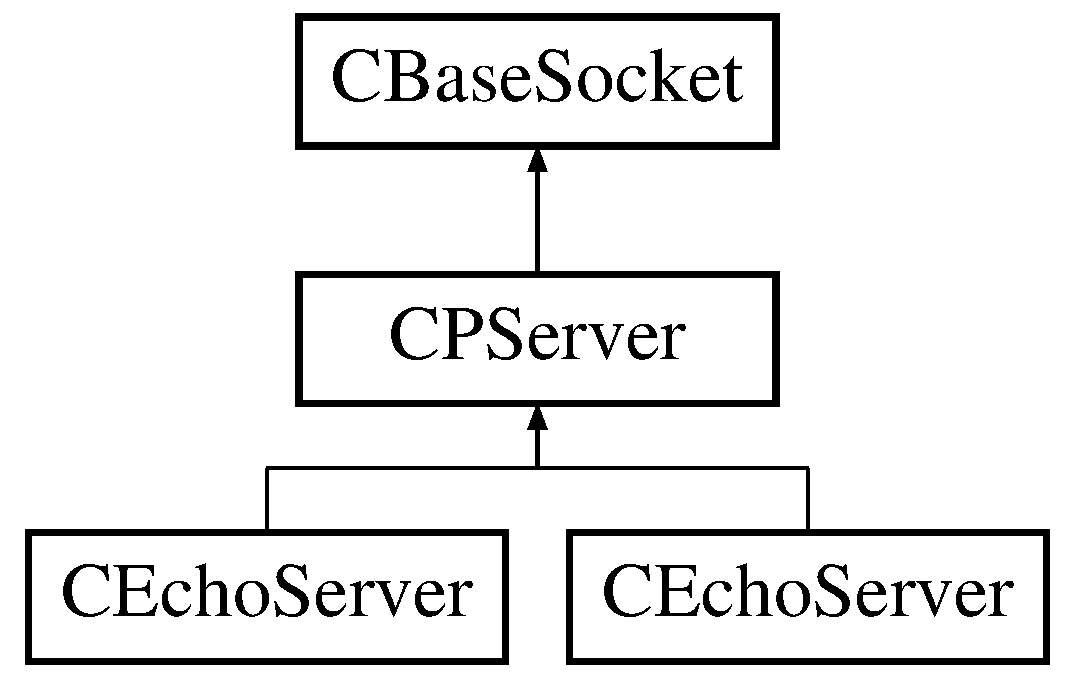
\includegraphics[height=3.000000cm]{class_c_p_server}
\end{center}
\end{figure}
\subsection*{\-Public \-Member \-Functions}
\begin{DoxyCompactItemize}
\item 
\hyperlink{class_c_p_server_a5adf5787e2cfb4ecfe86a0c18f2e1cb3}{\-C\-P\-Server} (\hyperlink{_c_p_connection_handler_8h_a05bf2fef946dbf14350a5f45bb28f953}{\-C\-P\-\_\-\-C\-O\-N\-N\-E\-C\-T\-I\-O\-N\-\_\-\-H\-A\-N\-D\-L\-E\-R\-\_\-\-A\-R\-R\-A\-Y} \&c\-P\-Connection\-Handlers)
\begin{DoxyCompactList}\small\item\em constructor \end{DoxyCompactList}\item 
virtual \hyperlink{class_c_p_server_a5698810878ce141158b4a9bf9dfeb4bf}{$\sim$\-C\-P\-Server} ()
\item 
\hyperlink{_cpclient_8h_a3be13892ae7076009afcf121347dd319}{\-B\-O\-O\-L} \hyperlink{class_c_p_server_a507f35f780de641c071bfd8a3f793a75}{\-Listen} (int n\-Connection\-Backlog=\-S\-O\-M\-A\-X\-C\-O\-N\-N)
\item 
\hyperlink{_cpclient_8h_a6464f7480a0fd0ee170cba12b2c0497f}{void} \hyperlink{class_c_p_server_ac7ed83bcdae44d824e4391861290b565}{\-Shutdown\-All} ()
\item 
time\-\_\-t \hyperlink{class_c_p_server_aa4a8f5591c3f63de66deff1d6b4a1c5e}{\-Get\-Time\-Started} ()
\end{DoxyCompactItemize}
\subsection*{\-Protected \-Member \-Functions}
\begin{DoxyCompactItemize}
\item 
virtual \hyperlink{_cpclient_8h_a6464f7480a0fd0ee170cba12b2c0497f}{void} \hyperlink{class_c_p_server_a09ac2e46ccc306c92b43bd556f682e81}{\-Cleanup\-Array} (\hyperlink{_cpclient_8h_a3be13892ae7076009afcf121347dd319}{\-B\-O\-O\-L} b\-Terminate\-All=\hyperlink{_x_plat_8h_aa93f0eb578d23995850d61f7d61c55c1}{\-F\-A\-L\-S\-E})
\begin{DoxyCompactList}\small\item\em \-Clean up array. \end{DoxyCompactList}\item 
virtual \hyperlink{_cpclient_8h_a3be13892ae7076009afcf121347dd319}{\-B\-O\-O\-L} \hyperlink{class_c_p_server_a1abdbfc0ef46eb052da96829d90a2420}{\-Accept} ()
\begin{DoxyCompactList}\small\item\em \-Accept connections. \end{DoxyCompactList}\item 
virtual \hyperlink{class_c_p_connection}{\-C\-P\-Connection} $\ast$ \hyperlink{class_c_p_server_ab028d102106a438f32c622596eaa1bc0}{\-Allocate\-Socket\-Class} (struct sockaddr $\ast$p\-Addr)=0
\end{DoxyCompactItemize}
\subsection*{\-Static \-Protected \-Member \-Functions}
\begin{DoxyCompactItemize}
\item 
static unsigned \hyperlink{class_c_p_server_a536d91cd5cc25f5bb120345c5ed0cd5b}{\-Accept\-Connection} (\hyperlink{_cpclient_8h_a6464f7480a0fd0ee170cba12b2c0497f}{void} $\ast$p\-Void)
\begin{DoxyCompactList}\small\item\em \-Listening thread. \end{DoxyCompactList}\end{DoxyCompactItemize}
\subsection*{\-Protected \-Attributes}
\begin{DoxyCompactItemize}
\item 
\hyperlink{_c_p_connection_handler_8h_a05bf2fef946dbf14350a5f45bb28f953}{\-C\-P\-\_\-\-C\-O\-N\-N\-E\-C\-T\-I\-O\-N\-\_\-\-H\-A\-N\-D\-L\-E\-R\-\_\-\-A\-R\-R\-A\-Y} \hyperlink{class_c_p_server_a1080e054402b166e08c38bdb0f92969a}{c\-Handlers}
\begin{DoxyCompactList}\small\item\em data member \end{DoxyCompactList}\item 
vector$<$ \hyperlink{class_c_p_connection}{\-C\-P\-Connection} $\ast$ $>$ \hyperlink{class_c_p_server_a5529eba58fcaf14f96b39895520b5468}{c\-Socket\-Array}
\begin{DoxyCompactList}\small\item\em \-Array of \hyperlink{class_c_p_connection}{\-C\-P\-Connection} objects created. \end{DoxyCompactList}\item 
\hyperlink{_x_plat_8h_af3c5c1485bb09f4be888d78cdaf93e00}{\-X\-P\-L\-A\-T\-\_\-\-H\-A\-N\-D\-L\-E} \hyperlink{class_c_p_server_aaff398bbe130c88c778231fb9dc163c6}{h\-Thread}
\item 
time\-\_\-t \hyperlink{class_c_p_server_a18665bfa95ace98f79d6e1b6b7a38398}{t\-Started}
\item 
\hyperlink{class_c_x_plat_critical_section}{\-C\-X\-Plat\-Critical\-Section} \hyperlink{class_c_p_server_a80980bd78734de4dc8fa48f5efdc502d}{c\-Crit\-Socket\-Array}
\item 
int \hyperlink{class_c_p_server_a1d016fb3e151466593bc3c16941bd222}{i\-Num\-Handlers}
\end{DoxyCompactItemize}


\subsection{\-Detailed \-Description}
\-C\-P\-Server.\-h\-: interface for the \hyperlink{class_c_p_server}{\-C\-P\-Server} class. 

\-\_\-\-M\-S\-C\-\_\-\-V\-E\-R $>$ 1000 \-Pooled connection server class. \-Handles multiple \-T\-C\-P connections with just a connection accept thread and an \-I/\-O thread, making it highly scalable 

\-Definition at line 34 of file \-Cpserver.\-h.



\subsection{\-Constructor \& \-Destructor \-Documentation}
\hypertarget{class_c_p_server_a5adf5787e2cfb4ecfe86a0c18f2e1cb3}{\index{\-C\-P\-Server@{\-C\-P\-Server}!\-C\-P\-Server@{\-C\-P\-Server}}
\index{\-C\-P\-Server@{\-C\-P\-Server}!CPServer@{\-C\-P\-Server}}
\subsubsection[{\-C\-P\-Server}]{\setlength{\rightskip}{0pt plus 5cm}{\bf \-C\-P\-Server\-::\-C\-P\-Server} (
\begin{DoxyParamCaption}
\item[{{\bf \-C\-P\-\_\-\-C\-O\-N\-N\-E\-C\-T\-I\-O\-N\-\_\-\-H\-A\-N\-D\-L\-E\-R\-\_\-\-A\-R\-R\-A\-Y} \&}]{c\-P\-Connection\-Handlers}
\end{DoxyParamCaption}
)}}\label{class_c_p_server_a5adf5787e2cfb4ecfe86a0c18f2e1cb3}


constructor 



\-Definition at line 33 of file \-Cpserver.\-cpp.

\hypertarget{class_c_p_server_a5698810878ce141158b4a9bf9dfeb4bf}{\index{\-C\-P\-Server@{\-C\-P\-Server}!$\sim$\-C\-P\-Server@{$\sim$\-C\-P\-Server}}
\index{$\sim$\-C\-P\-Server@{$\sim$\-C\-P\-Server}!CPServer@{\-C\-P\-Server}}
\subsubsection[{$\sim$\-C\-P\-Server}]{\setlength{\rightskip}{0pt plus 5cm}{\bf \-C\-P\-Server\-::$\sim$\-C\-P\-Server} (
\begin{DoxyParamCaption}
{}
\end{DoxyParamCaption}
)\hspace{0.3cm}{\ttfamily  \mbox{[}virtual\mbox{]}}}}\label{class_c_p_server_a5698810878ce141158b4a9bf9dfeb4bf}


\-Definition at line 41 of file \-Cpserver.\-cpp.



\subsection{\-Member \-Function \-Documentation}
\hypertarget{class_c_p_server_a1abdbfc0ef46eb052da96829d90a2420}{\index{\-C\-P\-Server@{\-C\-P\-Server}!\-Accept@{\-Accept}}
\index{\-Accept@{\-Accept}!CPServer@{\-C\-P\-Server}}
\subsubsection[{\-Accept}]{\setlength{\rightskip}{0pt plus 5cm}{\bf \-B\-O\-O\-L} {\bf \-C\-P\-Server\-::\-Accept} (
\begin{DoxyParamCaption}
{}
\end{DoxyParamCaption}
)\hspace{0.3cm}{\ttfamily  \mbox{[}protected, virtual\mbox{]}}}}\label{class_c_p_server_a1abdbfc0ef46eb052da96829d90a2420}


\-Accept connections. 



\-Definition at line 106 of file \-Cpserver.\-cpp.

\hypertarget{class_c_p_server_a536d91cd5cc25f5bb120345c5ed0cd5b}{\index{\-C\-P\-Server@{\-C\-P\-Server}!\-Accept\-Connection@{\-Accept\-Connection}}
\index{\-Accept\-Connection@{\-Accept\-Connection}!CPServer@{\-C\-P\-Server}}
\subsubsection[{\-Accept\-Connection}]{\setlength{\rightskip}{0pt plus 5cm}unsigned {\bf \-C\-P\-Server\-::\-Accept\-Connection} (
\begin{DoxyParamCaption}
\item[{{\bf void} $\ast$}]{p\-Void}
\end{DoxyParamCaption}
)\hspace{0.3cm}{\ttfamily  \mbox{[}static, protected\mbox{]}}}}\label{class_c_p_server_a536d91cd5cc25f5bb120345c5ed0cd5b}


\-Listening thread. 



\-Definition at line 310 of file \-Cpserver.\-cpp.

\hypertarget{class_c_p_server_ab028d102106a438f32c622596eaa1bc0}{\index{\-C\-P\-Server@{\-C\-P\-Server}!\-Allocate\-Socket\-Class@{\-Allocate\-Socket\-Class}}
\index{\-Allocate\-Socket\-Class@{\-Allocate\-Socket\-Class}!CPServer@{\-C\-P\-Server}}
\subsubsection[{\-Allocate\-Socket\-Class}]{\setlength{\rightskip}{0pt plus 5cm}virtual {\bf \-C\-P\-Connection}$\ast$ {\bf \-C\-P\-Server\-::\-Allocate\-Socket\-Class} (
\begin{DoxyParamCaption}
\item[{struct sockaddr $\ast$}]{p\-Addr}
\end{DoxyParamCaption}
)\hspace{0.3cm}{\ttfamily  \mbox{[}protected, pure virtual\mbox{]}}}}\label{class_c_p_server_ab028d102106a438f32c622596eaa1bc0}
\-Pure virtual functions allocate and dallocate a derivative of \hyperlink{class_c_connection_socket}{\-C\-Connection\-Socket} \-Redefine in derived class 

\-Implemented in \hyperlink{class_c_echo_server_a538eb049166aca7a0d27c7914c853876}{\-C\-Echo\-Server}, and \hyperlink{class_c_echo_server_a8db4489876af267711eefbfd891bbb4d}{\-C\-Echo\-Server}.

\hypertarget{class_c_p_server_a09ac2e46ccc306c92b43bd556f682e81}{\index{\-C\-P\-Server@{\-C\-P\-Server}!\-Cleanup\-Array@{\-Cleanup\-Array}}
\index{\-Cleanup\-Array@{\-Cleanup\-Array}!CPServer@{\-C\-P\-Server}}
\subsubsection[{\-Cleanup\-Array}]{\setlength{\rightskip}{0pt plus 5cm}{\bf void} {\bf \-C\-P\-Server\-::\-Cleanup\-Array} (
\begin{DoxyParamCaption}
\item[{{\bf \-B\-O\-O\-L}}]{b\-Terminate\-All = {\ttfamily {\bf \-F\-A\-L\-S\-E}}}
\end{DoxyParamCaption}
)\hspace{0.3cm}{\ttfamily  \mbox{[}protected, virtual\mbox{]}}}}\label{class_c_p_server_a09ac2e46ccc306c92b43bd556f682e81}


\-Clean up array. 



\-Definition at line 250 of file \-Cpserver.\-cpp.

\hypertarget{class_c_p_server_aa4a8f5591c3f63de66deff1d6b4a1c5e}{\index{\-C\-P\-Server@{\-C\-P\-Server}!\-Get\-Time\-Started@{\-Get\-Time\-Started}}
\index{\-Get\-Time\-Started@{\-Get\-Time\-Started}!CPServer@{\-C\-P\-Server}}
\subsubsection[{\-Get\-Time\-Started}]{\setlength{\rightskip}{0pt plus 5cm}time\-\_\-t {\bf \-C\-P\-Server\-::\-Get\-Time\-Started} (
\begin{DoxyParamCaption}
{}
\end{DoxyParamCaption}
)}}\label{class_c_p_server_aa4a8f5591c3f63de66deff1d6b4a1c5e}


\-Definition at line 321 of file \-Cpserver.\-cpp.

\hypertarget{class_c_p_server_a507f35f780de641c071bfd8a3f793a75}{\index{\-C\-P\-Server@{\-C\-P\-Server}!\-Listen@{\-Listen}}
\index{\-Listen@{\-Listen}!CPServer@{\-C\-P\-Server}}
\subsubsection[{\-Listen}]{\setlength{\rightskip}{0pt plus 5cm}{\bf \-B\-O\-O\-L} {\bf \-C\-P\-Server\-::\-Listen} (
\begin{DoxyParamCaption}
\item[{int}]{n\-Connection\-Backlog = {\ttfamily \-S\-O\-M\-A\-X\-C\-O\-N\-N}}
\end{DoxyParamCaption}
)}}\label{class_c_p_server_a507f35f780de641c071bfd8a3f793a75}


\-Definition at line 48 of file \-Cpserver.\-cpp.

\hypertarget{class_c_p_server_ac7ed83bcdae44d824e4391861290b565}{\index{\-C\-P\-Server@{\-C\-P\-Server}!\-Shutdown\-All@{\-Shutdown\-All}}
\index{\-Shutdown\-All@{\-Shutdown\-All}!CPServer@{\-C\-P\-Server}}
\subsubsection[{\-Shutdown\-All}]{\setlength{\rightskip}{0pt plus 5cm}{\bf void} {\bf \-C\-P\-Server\-::\-Shutdown\-All} (
\begin{DoxyParamCaption}
{}
\end{DoxyParamCaption}
)}}\label{class_c_p_server_ac7ed83bcdae44d824e4391861290b565}


\-Definition at line 292 of file \-Cpserver.\-cpp.



\subsection{\-Member \-Data \-Documentation}
\hypertarget{class_c_p_server_a80980bd78734de4dc8fa48f5efdc502d}{\index{\-C\-P\-Server@{\-C\-P\-Server}!c\-Crit\-Socket\-Array@{c\-Crit\-Socket\-Array}}
\index{c\-Crit\-Socket\-Array@{c\-Crit\-Socket\-Array}!CPServer@{\-C\-P\-Server}}
\subsubsection[{c\-Crit\-Socket\-Array}]{\setlength{\rightskip}{0pt plus 5cm}{\bf \-C\-X\-Plat\-Critical\-Section} {\bf \-C\-P\-Server\-::c\-Crit\-Socket\-Array}\hspace{0.3cm}{\ttfamily  \mbox{[}protected\mbox{]}}}}\label{class_c_p_server_a80980bd78734de4dc8fa48f5efdc502d}


\-Definition at line 68 of file \-Cpserver.\-h.

\hypertarget{class_c_p_server_a1080e054402b166e08c38bdb0f92969a}{\index{\-C\-P\-Server@{\-C\-P\-Server}!c\-Handlers@{c\-Handlers}}
\index{c\-Handlers@{c\-Handlers}!CPServer@{\-C\-P\-Server}}
\subsubsection[{c\-Handlers}]{\setlength{\rightskip}{0pt plus 5cm}{\bf \-C\-P\-\_\-\-C\-O\-N\-N\-E\-C\-T\-I\-O\-N\-\_\-\-H\-A\-N\-D\-L\-E\-R\-\_\-\-A\-R\-R\-A\-Y} {\bf \-C\-P\-Server\-::c\-Handlers}\hspace{0.3cm}{\ttfamily  \mbox{[}protected\mbox{]}}}}\label{class_c_p_server_a1080e054402b166e08c38bdb0f92969a}


data member 

\-Array of \-C\-P\-Connection\-Handlers. \-Use the one with the least connections. 

\-Definition at line 63 of file \-Cpserver.\-h.

\hypertarget{class_c_p_server_a5529eba58fcaf14f96b39895520b5468}{\index{\-C\-P\-Server@{\-C\-P\-Server}!c\-Socket\-Array@{c\-Socket\-Array}}
\index{c\-Socket\-Array@{c\-Socket\-Array}!CPServer@{\-C\-P\-Server}}
\subsubsection[{c\-Socket\-Array}]{\setlength{\rightskip}{0pt plus 5cm}vector$<${\bf \-C\-P\-Connection} $\ast$$>$ {\bf \-C\-P\-Server\-::c\-Socket\-Array}\hspace{0.3cm}{\ttfamily  \mbox{[}protected\mbox{]}}}}\label{class_c_p_server_a5529eba58fcaf14f96b39895520b5468}


\-Array of \hyperlink{class_c_p_connection}{\-C\-P\-Connection} objects created. 



\-Definition at line 65 of file \-Cpserver.\-h.

\hypertarget{class_c_p_server_aaff398bbe130c88c778231fb9dc163c6}{\index{\-C\-P\-Server@{\-C\-P\-Server}!h\-Thread@{h\-Thread}}
\index{h\-Thread@{h\-Thread}!CPServer@{\-C\-P\-Server}}
\subsubsection[{h\-Thread}]{\setlength{\rightskip}{0pt plus 5cm}{\bf \-X\-P\-L\-A\-T\-\_\-\-H\-A\-N\-D\-L\-E} {\bf \-C\-P\-Server\-::h\-Thread}\hspace{0.3cm}{\ttfamily  \mbox{[}protected\mbox{]}}}}\label{class_c_p_server_aaff398bbe130c88c778231fb9dc163c6}


\-Definition at line 66 of file \-Cpserver.\-h.

\hypertarget{class_c_p_server_a1d016fb3e151466593bc3c16941bd222}{\index{\-C\-P\-Server@{\-C\-P\-Server}!i\-Num\-Handlers@{i\-Num\-Handlers}}
\index{i\-Num\-Handlers@{i\-Num\-Handlers}!CPServer@{\-C\-P\-Server}}
\subsubsection[{i\-Num\-Handlers}]{\setlength{\rightskip}{0pt plus 5cm}int {\bf \-C\-P\-Server\-::i\-Num\-Handlers}\hspace{0.3cm}{\ttfamily  \mbox{[}protected\mbox{]}}}}\label{class_c_p_server_a1d016fb3e151466593bc3c16941bd222}


\-Definition at line 69 of file \-Cpserver.\-h.

\hypertarget{class_c_p_server_a18665bfa95ace98f79d6e1b6b7a38398}{\index{\-C\-P\-Server@{\-C\-P\-Server}!t\-Started@{t\-Started}}
\index{t\-Started@{t\-Started}!CPServer@{\-C\-P\-Server}}
\subsubsection[{t\-Started}]{\setlength{\rightskip}{0pt plus 5cm}time\-\_\-t {\bf \-C\-P\-Server\-::t\-Started}\hspace{0.3cm}{\ttfamily  \mbox{[}protected\mbox{]}}}}\label{class_c_p_server_a18665bfa95ace98f79d6e1b6b7a38398}


\-Definition at line 67 of file \-Cpserver.\-h.



\-The documentation for this class was generated from the following files\-:\begin{DoxyCompactItemize}
\item 
common/\hyperlink{_cpserver_8h}{\-Cpserver.\-h}\item 
common/\hyperlink{_cpserver_8cpp}{\-Cpserver.\-cpp}\end{DoxyCompactItemize}

\hypertarget{class_c_r_c32}{\section{\-C\-R\-C32 \-Class \-Reference}
\label{class_c_r_c32}\index{\-C\-R\-C32@{\-C\-R\-C32}}
}


{\ttfamily \#include $<$\-Crc32.\-h$>$}

\subsection*{\-Public \-Member \-Functions}
\begin{DoxyCompactItemize}
\item 
\hyperlink{class_c_r_c32_a450b845a91ef96b9e41cc1049cca52fc}{\-C\-R\-C32} ()
\item 
virtual \hyperlink{class_c_r_c32_a444ef004c9cdf62380638c157bf0a731}{$\sim$\-C\-R\-C32} ()
\item 
unsigned long \hyperlink{class_c_r_c32_ac2692eca4edeccc205aab20db05a12a1}{\-Calc\-C\-R\-C} (unsigned long l\-Init, unsigned char $\ast$lp\-Buffer, int i\-Length)
\end{DoxyCompactItemize}
\subsection*{\-Protected \-Attributes}
\begin{DoxyCompactItemize}
\item 
unsigned long \hyperlink{class_c_r_c32_a9bda31e70a6bbd94caa3b3a66a2674c8}{l\-Crc\-Table} \mbox{[}256\mbox{]}
\end{DoxyCompactItemize}


\subsection{\-Detailed \-Description}


\-Definition at line 23 of file \-Crc32.\-h.



\subsection{\-Constructor \& \-Destructor \-Documentation}
\hypertarget{class_c_r_c32_a450b845a91ef96b9e41cc1049cca52fc}{\index{\-C\-R\-C32@{\-C\-R\-C32}!\-C\-R\-C32@{\-C\-R\-C32}}
\index{\-C\-R\-C32@{\-C\-R\-C32}!CRC32@{\-C\-R\-C32}}
\subsubsection[{\-C\-R\-C32}]{\setlength{\rightskip}{0pt plus 5cm}{\bf \-C\-R\-C32\-::\-C\-R\-C32} (
\begin{DoxyParamCaption}
{}
\end{DoxyParamCaption}
)}}\label{class_c_r_c32_a450b845a91ef96b9e41cc1049cca52fc}


\-Definition at line 25 of file \-Crc32.\-cpp.

\hypertarget{class_c_r_c32_a444ef004c9cdf62380638c157bf0a731}{\index{\-C\-R\-C32@{\-C\-R\-C32}!$\sim$\-C\-R\-C32@{$\sim$\-C\-R\-C32}}
\index{$\sim$\-C\-R\-C32@{$\sim$\-C\-R\-C32}!CRC32@{\-C\-R\-C32}}
\subsubsection[{$\sim$\-C\-R\-C32}]{\setlength{\rightskip}{0pt plus 5cm}{\bf \-C\-R\-C32\-::$\sim$\-C\-R\-C32} (
\begin{DoxyParamCaption}
{}
\end{DoxyParamCaption}
)\hspace{0.3cm}{\ttfamily  \mbox{[}virtual\mbox{]}}}}\label{class_c_r_c32_a444ef004c9cdf62380638c157bf0a731}


\-Definition at line 47 of file \-Crc32.\-cpp.



\subsection{\-Member \-Function \-Documentation}
\hypertarget{class_c_r_c32_ac2692eca4edeccc205aab20db05a12a1}{\index{\-C\-R\-C32@{\-C\-R\-C32}!\-Calc\-C\-R\-C@{\-Calc\-C\-R\-C}}
\index{\-Calc\-C\-R\-C@{\-Calc\-C\-R\-C}!CRC32@{\-C\-R\-C32}}
\subsubsection[{\-Calc\-C\-R\-C}]{\setlength{\rightskip}{0pt plus 5cm}unsigned long {\bf \-C\-R\-C32\-::\-Calc\-C\-R\-C} (
\begin{DoxyParamCaption}
\item[{unsigned long}]{l\-Init, }
\item[{unsigned char $\ast$}]{lp\-Buffer, }
\item[{int}]{i\-Length}
\end{DoxyParamCaption}
)}}\label{class_c_r_c32_ac2692eca4edeccc205aab20db05a12a1}


\-Definition at line 53 of file \-Crc32.\-cpp.



\subsection{\-Member \-Data \-Documentation}
\hypertarget{class_c_r_c32_a9bda31e70a6bbd94caa3b3a66a2674c8}{\index{\-C\-R\-C32@{\-C\-R\-C32}!l\-Crc\-Table@{l\-Crc\-Table}}
\index{l\-Crc\-Table@{l\-Crc\-Table}!CRC32@{\-C\-R\-C32}}
\subsubsection[{l\-Crc\-Table}]{\setlength{\rightskip}{0pt plus 5cm}unsigned long {\bf \-C\-R\-C32\-::l\-Crc\-Table}\mbox{[}256\mbox{]}\hspace{0.3cm}{\ttfamily  \mbox{[}protected\mbox{]}}}}\label{class_c_r_c32_a9bda31e70a6bbd94caa3b3a66a2674c8}


\-Definition at line 33 of file \-Crc32.\-h.



\-The documentation for this class was generated from the following files\-:\begin{DoxyCompactItemize}
\item 
common/\hyperlink{_crc32_8h}{\-Crc32.\-h}\item 
common/\hyperlink{_crc32_8cpp}{\-Crc32.\-cpp}\end{DoxyCompactItemize}

\hypertarget{class_c_secure_file_i_o}{\section{\-C\-Secure\-File\-I\-O \-Class \-Reference}
\label{class_c_secure_file_i_o}\index{\-C\-Secure\-File\-I\-O@{\-C\-Secure\-File\-I\-O}}
}


\-Class to read and write a file using openssl encryption.  




{\ttfamily \#include $<$\-C\-Secure\-File\-I\-O.\-h$>$}

\subsection*{\-Public \-Member \-Functions}
\begin{DoxyCompactItemize}
\item 
\hyperlink{class_c_secure_file_i_o_a38da84ec9e56170cdfff609f3cbcc4f0}{\-C\-Secure\-File\-I\-O} ()
\item 
virtual \hyperlink{class_c_secure_file_i_o_ac4d83da8c95a9f864c9f89819f05219a}{$\sim$\-C\-Secure\-File\-I\-O} ()
\item 
int \hyperlink{class_c_secure_file_i_o_a329a8677443725b37ee21a291bf0d5db}{\-Read\-Encypted\-File} (const char $\ast$p\-File\-Path, string \&s\-Buffer)
\begin{DoxyCompactList}\small\item\em \-Retrieve an encrypted file. \-Returns bytes read or -\/1. \end{DoxyCompactList}\item 
int \hyperlink{class_c_secure_file_i_o_a6cc4fc174952e378eb86e96631bdcdc5}{\-Write\-Encypted\-File} (const char $\ast$p\-File\-Path, const char $\ast$p\-Buffer)
\begin{DoxyCompactList}\small\item\em \-Write an encrypted file. \-Returns bytes written or -\/1. \end{DoxyCompactList}\item 
\hyperlink{_cpclient_8h_a6464f7480a0fd0ee170cba12b2c0497f}{void} \hyperlink{class_c_secure_file_i_o_adee11b95c6772322bc421191b055a1a6}{\-B\-F\-\_\-encrypt} (const unsigned char $\ast$keydata, int keydatalen, unsigned char $\ast$in, unsigned char $\ast$out, unsigned int inlen)
\begin{DoxyCompactList}\small\item\em \-Encrypt buffer. \end{DoxyCompactList}\item 
\hyperlink{_cpclient_8h_a6464f7480a0fd0ee170cba12b2c0497f}{void} \hyperlink{class_c_secure_file_i_o_a2ab08cd2ca5f762108dec56ac15ba890}{\-B\-F\-\_\-decrypt} (const unsigned char $\ast$keydata, int keydatalen, unsigned char $\ast$in, unsigned char $\ast$out, unsigned int inlen)
\begin{DoxyCompactList}\small\item\em \-Decrypt buffer. \end{DoxyCompactList}\end{DoxyCompactItemize}
\subsection*{\-Public \-Attributes}
\begin{DoxyCompactItemize}
\item 
unsigned char $\ast$ \hyperlink{class_c_secure_file_i_o_a30dd558e0f000202e24b7633c3695156}{uc\-Key}
\item 
int \hyperlink{class_c_secure_file_i_o_af55ac7c269cc10201170359307c20542}{i\-Key\-Size}
\end{DoxyCompactItemize}


\subsection{\-Detailed \-Description}
\-Class to read and write a file using openssl encryption. 

\-Definition at line 20 of file \-C\-Secure\-File\-I\-O.\-h.



\subsection{\-Constructor \& \-Destructor \-Documentation}
\hypertarget{class_c_secure_file_i_o_a38da84ec9e56170cdfff609f3cbcc4f0}{\index{\-C\-Secure\-File\-I\-O@{\-C\-Secure\-File\-I\-O}!\-C\-Secure\-File\-I\-O@{\-C\-Secure\-File\-I\-O}}
\index{\-C\-Secure\-File\-I\-O@{\-C\-Secure\-File\-I\-O}!CSecureFileIO@{\-C\-Secure\-File\-I\-O}}
\subsubsection[{\-C\-Secure\-File\-I\-O}]{\setlength{\rightskip}{0pt plus 5cm}{\bf \-C\-Secure\-File\-I\-O\-::\-C\-Secure\-File\-I\-O} (
\begin{DoxyParamCaption}
{}
\end{DoxyParamCaption}
)}}\label{class_c_secure_file_i_o_a38da84ec9e56170cdfff609f3cbcc4f0}


\-Definition at line 14 of file \-C\-Secure\-File\-I\-O.\-cpp.

\hypertarget{class_c_secure_file_i_o_ac4d83da8c95a9f864c9f89819f05219a}{\index{\-C\-Secure\-File\-I\-O@{\-C\-Secure\-File\-I\-O}!$\sim$\-C\-Secure\-File\-I\-O@{$\sim$\-C\-Secure\-File\-I\-O}}
\index{$\sim$\-C\-Secure\-File\-I\-O@{$\sim$\-C\-Secure\-File\-I\-O}!CSecureFileIO@{\-C\-Secure\-File\-I\-O}}
\subsubsection[{$\sim$\-C\-Secure\-File\-I\-O}]{\setlength{\rightskip}{0pt plus 5cm}{\bf \-C\-Secure\-File\-I\-O\-::$\sim$\-C\-Secure\-File\-I\-O} (
\begin{DoxyParamCaption}
{}
\end{DoxyParamCaption}
)\hspace{0.3cm}{\ttfamily  \mbox{[}virtual\mbox{]}}}}\label{class_c_secure_file_i_o_ac4d83da8c95a9f864c9f89819f05219a}


\-Definition at line 49 of file \-C\-Secure\-File\-I\-O.\-cpp.



\subsection{\-Member \-Function \-Documentation}
\hypertarget{class_c_secure_file_i_o_a2ab08cd2ca5f762108dec56ac15ba890}{\index{\-C\-Secure\-File\-I\-O@{\-C\-Secure\-File\-I\-O}!\-B\-F\-\_\-decrypt@{\-B\-F\-\_\-decrypt}}
\index{\-B\-F\-\_\-decrypt@{\-B\-F\-\_\-decrypt}!CSecureFileIO@{\-C\-Secure\-File\-I\-O}}
\subsubsection[{\-B\-F\-\_\-decrypt}]{\setlength{\rightskip}{0pt plus 5cm}{\bf void} {\bf \-C\-Secure\-File\-I\-O\-::\-B\-F\-\_\-decrypt} (
\begin{DoxyParamCaption}
\item[{const unsigned char $\ast$}]{keydata, }
\item[{int}]{keydatalen, }
\item[{unsigned char $\ast$}]{in, }
\item[{unsigned char $\ast$}]{out, }
\item[{unsigned int}]{inlen}
\end{DoxyParamCaption}
)}}\label{class_c_secure_file_i_o_a2ab08cd2ca5f762108dec56ac15ba890}


\-Decrypt buffer. 



\-Definition at line 153 of file \-C\-Secure\-File\-I\-O.\-cpp.

\hypertarget{class_c_secure_file_i_o_adee11b95c6772322bc421191b055a1a6}{\index{\-C\-Secure\-File\-I\-O@{\-C\-Secure\-File\-I\-O}!\-B\-F\-\_\-encrypt@{\-B\-F\-\_\-encrypt}}
\index{\-B\-F\-\_\-encrypt@{\-B\-F\-\_\-encrypt}!CSecureFileIO@{\-C\-Secure\-File\-I\-O}}
\subsubsection[{\-B\-F\-\_\-encrypt}]{\setlength{\rightskip}{0pt plus 5cm}{\bf void} {\bf \-C\-Secure\-File\-I\-O\-::\-B\-F\-\_\-encrypt} (
\begin{DoxyParamCaption}
\item[{const unsigned char $\ast$}]{keydata, }
\item[{int}]{keydatalen, }
\item[{unsigned char $\ast$}]{in, }
\item[{unsigned char $\ast$}]{out, }
\item[{unsigned int}]{inlen}
\end{DoxyParamCaption}
)}}\label{class_c_secure_file_i_o_adee11b95c6772322bc421191b055a1a6}


\-Encrypt buffer. 



\-Definition at line 141 of file \-C\-Secure\-File\-I\-O.\-cpp.

\hypertarget{class_c_secure_file_i_o_a329a8677443725b37ee21a291bf0d5db}{\index{\-C\-Secure\-File\-I\-O@{\-C\-Secure\-File\-I\-O}!\-Read\-Encypted\-File@{\-Read\-Encypted\-File}}
\index{\-Read\-Encypted\-File@{\-Read\-Encypted\-File}!CSecureFileIO@{\-C\-Secure\-File\-I\-O}}
\subsubsection[{\-Read\-Encypted\-File}]{\setlength{\rightskip}{0pt plus 5cm}int {\bf \-C\-Secure\-File\-I\-O\-::\-Read\-Encypted\-File} (
\begin{DoxyParamCaption}
\item[{const char $\ast$}]{p\-File\-Path, }
\item[{string \&}]{s\-Buffer}
\end{DoxyParamCaption}
)}}\label{class_c_secure_file_i_o_a329a8677443725b37ee21a291bf0d5db}


\-Retrieve an encrypted file. \-Returns bytes read or -\/1. 



\-Definition at line 57 of file \-C\-Secure\-File\-I\-O.\-cpp.

\hypertarget{class_c_secure_file_i_o_a6cc4fc174952e378eb86e96631bdcdc5}{\index{\-C\-Secure\-File\-I\-O@{\-C\-Secure\-File\-I\-O}!\-Write\-Encypted\-File@{\-Write\-Encypted\-File}}
\index{\-Write\-Encypted\-File@{\-Write\-Encypted\-File}!CSecureFileIO@{\-C\-Secure\-File\-I\-O}}
\subsubsection[{\-Write\-Encypted\-File}]{\setlength{\rightskip}{0pt plus 5cm}int {\bf \-C\-Secure\-File\-I\-O\-::\-Write\-Encypted\-File} (
\begin{DoxyParamCaption}
\item[{const char $\ast$}]{p\-File\-Path, }
\item[{const char $\ast$}]{p\-Buffer}
\end{DoxyParamCaption}
)}}\label{class_c_secure_file_i_o_a6cc4fc174952e378eb86e96631bdcdc5}


\-Write an encrypted file. \-Returns bytes written or -\/1. 



\-Definition at line 105 of file \-C\-Secure\-File\-I\-O.\-cpp.



\subsection{\-Member \-Data \-Documentation}
\hypertarget{class_c_secure_file_i_o_af55ac7c269cc10201170359307c20542}{\index{\-C\-Secure\-File\-I\-O@{\-C\-Secure\-File\-I\-O}!i\-Key\-Size@{i\-Key\-Size}}
\index{i\-Key\-Size@{i\-Key\-Size}!CSecureFileIO@{\-C\-Secure\-File\-I\-O}}
\subsubsection[{i\-Key\-Size}]{\setlength{\rightskip}{0pt plus 5cm}int {\bf \-C\-Secure\-File\-I\-O\-::i\-Key\-Size}}}\label{class_c_secure_file_i_o_af55ac7c269cc10201170359307c20542}


\-Definition at line 39 of file \-C\-Secure\-File\-I\-O.\-h.

\hypertarget{class_c_secure_file_i_o_a30dd558e0f000202e24b7633c3695156}{\index{\-C\-Secure\-File\-I\-O@{\-C\-Secure\-File\-I\-O}!uc\-Key@{uc\-Key}}
\index{uc\-Key@{uc\-Key}!CSecureFileIO@{\-C\-Secure\-File\-I\-O}}
\subsubsection[{uc\-Key}]{\setlength{\rightskip}{0pt plus 5cm}unsigned char$\ast$ {\bf \-C\-Secure\-File\-I\-O\-::uc\-Key}}}\label{class_c_secure_file_i_o_a30dd558e0f000202e24b7633c3695156}


\-Definition at line 38 of file \-C\-Secure\-File\-I\-O.\-h.



\-The documentation for this class was generated from the following files\-:\begin{DoxyCompactItemize}
\item 
common/\hyperlink{_c_secure_file_i_o_8h}{\-C\-Secure\-File\-I\-O.\-h}\item 
common/\hyperlink{_c_secure_file_i_o_8cpp}{\-C\-Secure\-File\-I\-O.\-cpp}\end{DoxyCompactItemize}

\hypertarget{class_c_server_socket}{\section{\-C\-Server\-Socket \-Class \-Reference}
\label{class_c_server_socket}\index{\-C\-Server\-Socket@{\-C\-Server\-Socket}}
}


\-Server socket listens to establish a connection.  




{\ttfamily \#include $<$\-C\-Server\-Socket.\-h$>$}

\-Inheritance diagram for \-C\-Server\-Socket\-:\begin{figure}[H]
\begin{center}
\leavevmode
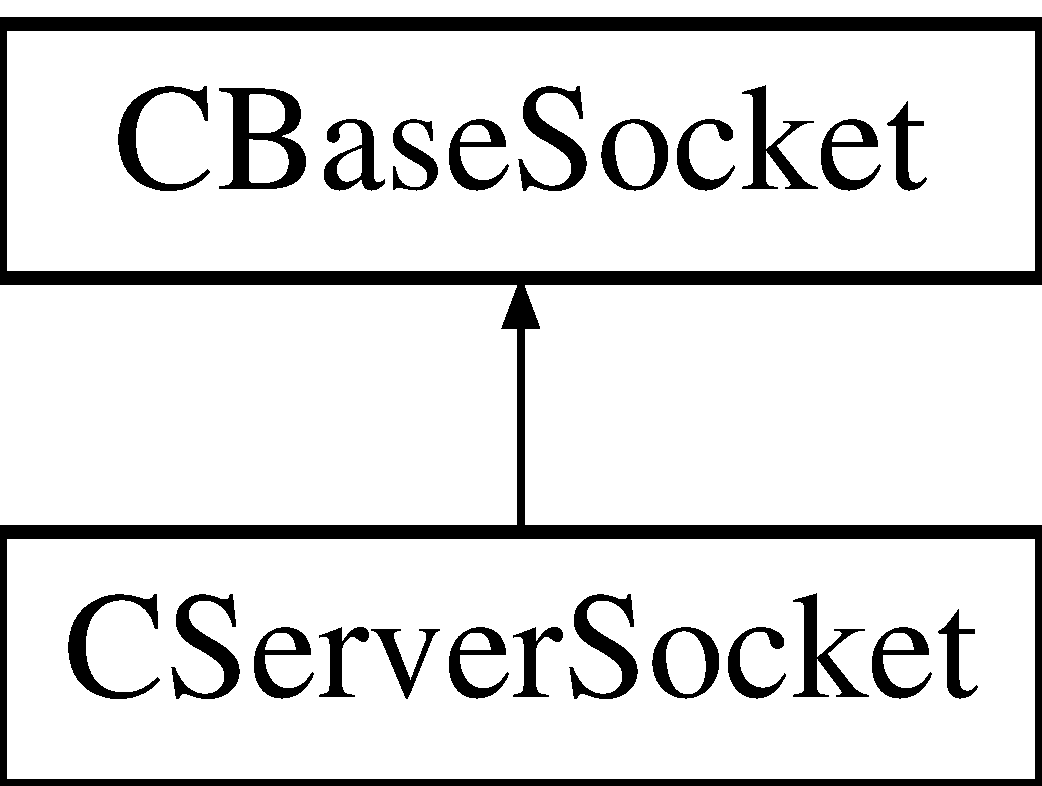
\includegraphics[height=2.000000cm]{class_c_server_socket}
\end{center}
\end{figure}
\subsection*{\-Public \-Member \-Functions}
\begin{DoxyCompactItemize}
\item 
\hyperlink{class_c_server_socket_a3ad9f83aa8aace5b319901abcc3b294b}{\-C\-Server\-Socket} ()
\begin{DoxyCompactList}\small\item\em constructor \end{DoxyCompactList}\item 
virtual \hyperlink{class_c_server_socket_a2efd5612c3e0258a6c3bb4fccca80bde}{$\sim$\-C\-Server\-Socket} ()
\item 
\hyperlink{_cpclient_8h_a3be13892ae7076009afcf121347dd319}{\-B\-O\-O\-L} \hyperlink{class_c_server_socket_a0cd67eacfd95ead6bdc8dab72464a5af}{\-Listen} (int n\-Connection\-Backlog=5)
\begin{DoxyCompactList}\small\item\em methods \end{DoxyCompactList}\item 
\hyperlink{_cpclient_8h_a6464f7480a0fd0ee170cba12b2c0497f}{void} \hyperlink{class_c_server_socket_a3992fdf11a055394a230044609d0f73e}{\-Shutdown\-All} ()
\item 
time\-\_\-t \hyperlink{class_c_server_socket_a52af0d07399deab64d56dfe10d81982b}{\-Get\-Time\-Started} ()
\item 
\hyperlink{_cpclient_8h_a6464f7480a0fd0ee170cba12b2c0497f}{void} \hyperlink{class_c_server_socket_a69e9bf0bcdf51797df78cf595cd5c528}{\-Wait\-For\-Exit} ()
\begin{DoxyCompactList}\small\item\em \-Wait for listening thread to exit. \end{DoxyCompactList}\end{DoxyCompactItemize}
\subsection*{\-Protected \-Member \-Functions}
\begin{DoxyCompactItemize}
\item 
virtual \hyperlink{_cpclient_8h_a6464f7480a0fd0ee170cba12b2c0497f}{void} \hyperlink{class_c_server_socket_aa6bbfa1461e437aa5ab864ee35016aa2}{\-Cleanup\-Array} (\hyperlink{_cpclient_8h_a3be13892ae7076009afcf121347dd319}{\-B\-O\-O\-L} b\-Terminate\-All=\hyperlink{_x_plat_8h_aa93f0eb578d23995850d61f7d61c55c1}{\-F\-A\-L\-S\-E})
\begin{DoxyCompactList}\small\item\em \-Clean up array. \end{DoxyCompactList}\item 
virtual \hyperlink{_cpclient_8h_a3be13892ae7076009afcf121347dd319}{\-B\-O\-O\-L} \hyperlink{class_c_server_socket_a3f1a261c6881f150caebd4389233382b}{\-Accept} ()
\begin{DoxyCompactList}\small\item\em \-Accept connections. \end{DoxyCompactList}\item 
virtual \hyperlink{class_c_connection_socket}{\-C\-Connection\-Socket} $\ast$ \hyperlink{class_c_server_socket_a5d9a8ba74dff11d71a2090c3fdf7c84a}{\-Allocate\-Socket\-Class} (struct sockaddr $\ast$p\-Addr)=0
\end{DoxyCompactItemize}
\subsection*{\-Static \-Protected \-Member \-Functions}
\begin{DoxyCompactItemize}
\item 
static unsigned \hyperlink{class_c_server_socket_a2290c6ce8fa0b268d9c89889a9e3eb89}{\-Accept\-Connection} (\hyperlink{_cpclient_8h_a6464f7480a0fd0ee170cba12b2c0497f}{void} $\ast$p\-Void)
\begin{DoxyCompactList}\small\item\em \-Listening thread. \end{DoxyCompactList}\end{DoxyCompactItemize}
\subsection*{\-Protected \-Attributes}
\begin{DoxyCompactItemize}
\item 
vector$<$ \hyperlink{_cpclient_8h_a6464f7480a0fd0ee170cba12b2c0497f}{void} $\ast$ $>$ \hyperlink{class_c_server_socket_ad231ce44c641ab0b3fa4c0087ea1400e}{c\-Socket\-Array}
\begin{DoxyCompactList}\small\item\em data member \end{DoxyCompactList}\item 
\hyperlink{_x_plat_8h_af3c5c1485bb09f4be888d78cdaf93e00}{\-X\-P\-L\-A\-T\-\_\-\-H\-A\-N\-D\-L\-E} \hyperlink{class_c_server_socket_ab42e0206af0388d76aafa6ea9a5e8038}{h\-Thread}
\item 
time\-\_\-t \hyperlink{class_c_server_socket_afb05d7651f4d59fdb791e1356721b764}{t\-Started}
\item 
\hyperlink{class_c_x_plat_critical_section}{\-C\-X\-Plat\-Critical\-Section} \hyperlink{class_c_server_socket_a5b6e77b060ed31986a6a36a5f18c65b8}{c\-Crit\-Socket\-Array}
\end{DoxyCompactItemize}


\subsection{\-Detailed \-Description}
\-Server socket listens to establish a connection. 

\-T\-C\-P socket server class 

\-Definition at line 27 of file \-C\-Server\-Socket.\-h.



\subsection{\-Constructor \& \-Destructor \-Documentation}
\hypertarget{class_c_server_socket_a3ad9f83aa8aace5b319901abcc3b294b}{\index{\-C\-Server\-Socket@{\-C\-Server\-Socket}!\-C\-Server\-Socket@{\-C\-Server\-Socket}}
\index{\-C\-Server\-Socket@{\-C\-Server\-Socket}!CServerSocket@{\-C\-Server\-Socket}}
\subsubsection[{\-C\-Server\-Socket}]{\setlength{\rightskip}{0pt plus 5cm}{\bf \-C\-Server\-Socket\-::\-C\-Server\-Socket} (
\begin{DoxyParamCaption}
{}
\end{DoxyParamCaption}
)}}\label{class_c_server_socket_a3ad9f83aa8aace5b319901abcc3b294b}


constructor 



\-Definition at line 29 of file \-C\-Server\-Socket.\-cpp.

\hypertarget{class_c_server_socket_a2efd5612c3e0258a6c3bb4fccca80bde}{\index{\-C\-Server\-Socket@{\-C\-Server\-Socket}!$\sim$\-C\-Server\-Socket@{$\sim$\-C\-Server\-Socket}}
\index{$\sim$\-C\-Server\-Socket@{$\sim$\-C\-Server\-Socket}!CServerSocket@{\-C\-Server\-Socket}}
\subsubsection[{$\sim$\-C\-Server\-Socket}]{\setlength{\rightskip}{0pt plus 5cm}{\bf \-C\-Server\-Socket\-::$\sim$\-C\-Server\-Socket} (
\begin{DoxyParamCaption}
{}
\end{DoxyParamCaption}
)\hspace{0.3cm}{\ttfamily  \mbox{[}virtual\mbox{]}}}}\label{class_c_server_socket_a2efd5612c3e0258a6c3bb4fccca80bde}


\-Definition at line 35 of file \-C\-Server\-Socket.\-cpp.



\subsection{\-Member \-Function \-Documentation}
\hypertarget{class_c_server_socket_a3f1a261c6881f150caebd4389233382b}{\index{\-C\-Server\-Socket@{\-C\-Server\-Socket}!\-Accept@{\-Accept}}
\index{\-Accept@{\-Accept}!CServerSocket@{\-C\-Server\-Socket}}
\subsubsection[{\-Accept}]{\setlength{\rightskip}{0pt plus 5cm}{\bf \-B\-O\-O\-L} {\bf \-C\-Server\-Socket\-::\-Accept} (
\begin{DoxyParamCaption}
{}
\end{DoxyParamCaption}
)\hspace{0.3cm}{\ttfamily  \mbox{[}protected, virtual\mbox{]}}}}\label{class_c_server_socket_a3f1a261c6881f150caebd4389233382b}


\-Accept connections. 



\-Definition at line 99 of file \-C\-Server\-Socket.\-cpp.

\hypertarget{class_c_server_socket_a2290c6ce8fa0b268d9c89889a9e3eb89}{\index{\-C\-Server\-Socket@{\-C\-Server\-Socket}!\-Accept\-Connection@{\-Accept\-Connection}}
\index{\-Accept\-Connection@{\-Accept\-Connection}!CServerSocket@{\-C\-Server\-Socket}}
\subsubsection[{\-Accept\-Connection}]{\setlength{\rightskip}{0pt plus 5cm}unsigned {\bf \-C\-Server\-Socket\-::\-Accept\-Connection} (
\begin{DoxyParamCaption}
\item[{{\bf void} $\ast$}]{p\-Void}
\end{DoxyParamCaption}
)\hspace{0.3cm}{\ttfamily  \mbox{[}static, protected\mbox{]}}}}\label{class_c_server_socket_a2290c6ce8fa0b268d9c89889a9e3eb89}


\-Listening thread. 



\-Definition at line 280 of file \-C\-Server\-Socket.\-cpp.

\hypertarget{class_c_server_socket_a5d9a8ba74dff11d71a2090c3fdf7c84a}{\index{\-C\-Server\-Socket@{\-C\-Server\-Socket}!\-Allocate\-Socket\-Class@{\-Allocate\-Socket\-Class}}
\index{\-Allocate\-Socket\-Class@{\-Allocate\-Socket\-Class}!CServerSocket@{\-C\-Server\-Socket}}
\subsubsection[{\-Allocate\-Socket\-Class}]{\setlength{\rightskip}{0pt plus 5cm}virtual {\bf \-C\-Connection\-Socket}$\ast$ {\bf \-C\-Server\-Socket\-::\-Allocate\-Socket\-Class} (
\begin{DoxyParamCaption}
\item[{struct sockaddr $\ast$}]{p\-Addr}
\end{DoxyParamCaption}
)\hspace{0.3cm}{\ttfamily  \mbox{[}protected, pure virtual\mbox{]}}}}\label{class_c_server_socket_a5d9a8ba74dff11d71a2090c3fdf7c84a}
\-Pure virtual functions allocate and dallocate a derivative of \hyperlink{class_c_connection_socket}{\-C\-Connection\-Socket} \-Redefine in derived class \hypertarget{class_c_server_socket_aa6bbfa1461e437aa5ab864ee35016aa2}{\index{\-C\-Server\-Socket@{\-C\-Server\-Socket}!\-Cleanup\-Array@{\-Cleanup\-Array}}
\index{\-Cleanup\-Array@{\-Cleanup\-Array}!CServerSocket@{\-C\-Server\-Socket}}
\subsubsection[{\-Cleanup\-Array}]{\setlength{\rightskip}{0pt plus 5cm}{\bf void} {\bf \-C\-Server\-Socket\-::\-Cleanup\-Array} (
\begin{DoxyParamCaption}
\item[{{\bf \-B\-O\-O\-L}}]{b\-Terminate\-All = {\ttfamily {\bf \-F\-A\-L\-S\-E}}}
\end{DoxyParamCaption}
)\hspace{0.3cm}{\ttfamily  \mbox{[}protected, virtual\mbox{]}}}}\label{class_c_server_socket_aa6bbfa1461e437aa5ab864ee35016aa2}


\-Clean up array. 



\-Definition at line 217 of file \-C\-Server\-Socket.\-cpp.

\hypertarget{class_c_server_socket_a52af0d07399deab64d56dfe10d81982b}{\index{\-C\-Server\-Socket@{\-C\-Server\-Socket}!\-Get\-Time\-Started@{\-Get\-Time\-Started}}
\index{\-Get\-Time\-Started@{\-Get\-Time\-Started}!CServerSocket@{\-C\-Server\-Socket}}
\subsubsection[{\-Get\-Time\-Started}]{\setlength{\rightskip}{0pt plus 5cm}time\-\_\-t {\bf \-C\-Server\-Socket\-::\-Get\-Time\-Started} (
\begin{DoxyParamCaption}
{}
\end{DoxyParamCaption}
)}}\label{class_c_server_socket_a52af0d07399deab64d56dfe10d81982b}


\-Definition at line 292 of file \-C\-Server\-Socket.\-cpp.

\hypertarget{class_c_server_socket_a0cd67eacfd95ead6bdc8dab72464a5af}{\index{\-C\-Server\-Socket@{\-C\-Server\-Socket}!\-Listen@{\-Listen}}
\index{\-Listen@{\-Listen}!CServerSocket@{\-C\-Server\-Socket}}
\subsubsection[{\-Listen}]{\setlength{\rightskip}{0pt plus 5cm}{\bf \-B\-O\-O\-L} {\bf \-C\-Server\-Socket\-::\-Listen} (
\begin{DoxyParamCaption}
\item[{int}]{n\-Connection\-Backlog = {\ttfamily 5}}
\end{DoxyParamCaption}
)}}\label{class_c_server_socket_a0cd67eacfd95ead6bdc8dab72464a5af}


methods 



\-Definition at line 44 of file \-C\-Server\-Socket.\-cpp.

\hypertarget{class_c_server_socket_a3992fdf11a055394a230044609d0f73e}{\index{\-C\-Server\-Socket@{\-C\-Server\-Socket}!\-Shutdown\-All@{\-Shutdown\-All}}
\index{\-Shutdown\-All@{\-Shutdown\-All}!CServerSocket@{\-C\-Server\-Socket}}
\subsubsection[{\-Shutdown\-All}]{\setlength{\rightskip}{0pt plus 5cm}{\bf void} {\bf \-C\-Server\-Socket\-::\-Shutdown\-All} (
\begin{DoxyParamCaption}
{}
\end{DoxyParamCaption}
)}}\label{class_c_server_socket_a3992fdf11a055394a230044609d0f73e}


\-Definition at line 261 of file \-C\-Server\-Socket.\-cpp.

\hypertarget{class_c_server_socket_a69e9bf0bcdf51797df78cf595cd5c528}{\index{\-C\-Server\-Socket@{\-C\-Server\-Socket}!\-Wait\-For\-Exit@{\-Wait\-For\-Exit}}
\index{\-Wait\-For\-Exit@{\-Wait\-For\-Exit}!CServerSocket@{\-C\-Server\-Socket}}
\subsubsection[{\-Wait\-For\-Exit}]{\setlength{\rightskip}{0pt plus 5cm}{\bf void} {\bf \-C\-Server\-Socket\-::\-Wait\-For\-Exit} (
\begin{DoxyParamCaption}
{}
\end{DoxyParamCaption}
)}}\label{class_c_server_socket_a69e9bf0bcdf51797df78cf595cd5c528}


\-Wait for listening thread to exit. 



\-Definition at line 300 of file \-C\-Server\-Socket.\-cpp.



\subsection{\-Member \-Data \-Documentation}
\hypertarget{class_c_server_socket_a5b6e77b060ed31986a6a36a5f18c65b8}{\index{\-C\-Server\-Socket@{\-C\-Server\-Socket}!c\-Crit\-Socket\-Array@{c\-Crit\-Socket\-Array}}
\index{c\-Crit\-Socket\-Array@{c\-Crit\-Socket\-Array}!CServerSocket@{\-C\-Server\-Socket}}
\subsubsection[{c\-Crit\-Socket\-Array}]{\setlength{\rightskip}{0pt plus 5cm}{\bf \-C\-X\-Plat\-Critical\-Section} {\bf \-C\-Server\-Socket\-::c\-Crit\-Socket\-Array}\hspace{0.3cm}{\ttfamily  \mbox{[}protected\mbox{]}}}}\label{class_c_server_socket_a5b6e77b060ed31986a6a36a5f18c65b8}


\-Definition at line 62 of file \-C\-Server\-Socket.\-h.

\hypertarget{class_c_server_socket_ad231ce44c641ab0b3fa4c0087ea1400e}{\index{\-C\-Server\-Socket@{\-C\-Server\-Socket}!c\-Socket\-Array@{c\-Socket\-Array}}
\index{c\-Socket\-Array@{c\-Socket\-Array}!CServerSocket@{\-C\-Server\-Socket}}
\subsubsection[{c\-Socket\-Array}]{\setlength{\rightskip}{0pt plus 5cm}vector$<${\bf void} $\ast$$>$ {\bf \-C\-Server\-Socket\-::c\-Socket\-Array}\hspace{0.3cm}{\ttfamily  \mbox{[}protected\mbox{]}}}}\label{class_c_server_socket_ad231ce44c641ab0b3fa4c0087ea1400e}


data member 

\-Array of \hyperlink{class_c_connection_socket}{\-C\-Connection\-Socket} objects created 

\-Definition at line 59 of file \-C\-Server\-Socket.\-h.

\hypertarget{class_c_server_socket_ab42e0206af0388d76aafa6ea9a5e8038}{\index{\-C\-Server\-Socket@{\-C\-Server\-Socket}!h\-Thread@{h\-Thread}}
\index{h\-Thread@{h\-Thread}!CServerSocket@{\-C\-Server\-Socket}}
\subsubsection[{h\-Thread}]{\setlength{\rightskip}{0pt plus 5cm}{\bf \-X\-P\-L\-A\-T\-\_\-\-H\-A\-N\-D\-L\-E} {\bf \-C\-Server\-Socket\-::h\-Thread}\hspace{0.3cm}{\ttfamily  \mbox{[}protected\mbox{]}}}}\label{class_c_server_socket_ab42e0206af0388d76aafa6ea9a5e8038}


\-Definition at line 60 of file \-C\-Server\-Socket.\-h.

\hypertarget{class_c_server_socket_afb05d7651f4d59fdb791e1356721b764}{\index{\-C\-Server\-Socket@{\-C\-Server\-Socket}!t\-Started@{t\-Started}}
\index{t\-Started@{t\-Started}!CServerSocket@{\-C\-Server\-Socket}}
\subsubsection[{t\-Started}]{\setlength{\rightskip}{0pt plus 5cm}time\-\_\-t {\bf \-C\-Server\-Socket\-::t\-Started}\hspace{0.3cm}{\ttfamily  \mbox{[}protected\mbox{]}}}}\label{class_c_server_socket_afb05d7651f4d59fdb791e1356721b764}


\-Definition at line 61 of file \-C\-Server\-Socket.\-h.



\-The documentation for this class was generated from the following files\-:\begin{DoxyCompactItemize}
\item 
common/\hyperlink{_c_server_socket_8h}{\-C\-Server\-Socket.\-h}\item 
common/\hyperlink{_c_server_socket_8cpp}{\-C\-Server\-Socket.\-cpp}\end{DoxyCompactItemize}

\hypertarget{class_c_spore_encrypt}{\section{\-C\-Spore\-Encrypt \-Class \-Reference}
\label{class_c_spore_encrypt}\index{\-C\-Spore\-Encrypt@{\-C\-Spore\-Encrypt}}
}


\-Class to encrypt data.  




{\ttfamily \#include $<$\-C\-Spore\-Encrypt.\-h$>$}

\subsection*{\-Public \-Member \-Functions}
\begin{DoxyCompactItemize}
\item 
\hyperlink{class_c_spore_encrypt_a6e14ddd8318a19377f0495c1dde02d12}{\-C\-Spore\-Encrypt} ()
\item 
virtual \hyperlink{class_c_spore_encrypt_a329bba299e2830874dff58a6a8fd06e0}{$\sim$\-C\-Spore\-Encrypt} ()
\end{DoxyCompactItemize}
\subsection*{\-Static \-Public \-Member \-Functions}
\begin{DoxyCompactItemize}
\item 
static \hyperlink{_cpclient_8h_a6464f7480a0fd0ee170cba12b2c0497f}{void} \hyperlink{class_c_spore_encrypt_a86040e68be4b03236eb4effbbd267239}{\-B\-F\-\_\-encrypt} (const unsigned char $\ast$keydata, int keydatalen, unsigned char $\ast$in, unsigned char $\ast$out, unsigned int inlen)
\begin{DoxyCompactList}\small\item\em \-Encrypt buffer. \end{DoxyCompactList}\item 
static \hyperlink{_cpclient_8h_a6464f7480a0fd0ee170cba12b2c0497f}{void} \hyperlink{class_c_spore_encrypt_a7dbc2b457ebf62ed52d4f004254914e9}{\-B\-F\-\_\-decrypt} (const unsigned char $\ast$keydata, int keydatalen, unsigned char $\ast$in, unsigned char $\ast$out, unsigned int inlen)
\begin{DoxyCompactList}\small\item\em \-Decrypt buffer. \end{DoxyCompactList}\end{DoxyCompactItemize}
\subsection*{\-Static \-Public \-Attributes}
\begin{DoxyCompactItemize}
\item 
static int \hyperlink{class_c_spore_encrypt_a6a83763486e61a888a59470f4d49a92f}{i\-Key\-Size} = 0
\item 
static unsigned char $\ast$ \hyperlink{class_c_spore_encrypt_ace12b5cef18687d97bab31ea9ebfb787}{uc\-Key} = \-N\-U\-L\-L
\end{DoxyCompactItemize}
\subsection*{\-Static \-Protected \-Member \-Functions}
\begin{DoxyCompactItemize}
\item 
static \hyperlink{_cpclient_8h_a6464f7480a0fd0ee170cba12b2c0497f}{void} \hyperlink{class_c_spore_encrypt_a89e49dc2b208c23d0072730ca5b5436a}{\-Get\-Key} ()
\end{DoxyCompactItemize}


\subsection{\-Detailed \-Description}
\-Class to encrypt data. 

\-Definition at line 17 of file \-C\-Spore\-Encrypt.\-h.



\subsection{\-Constructor \& \-Destructor \-Documentation}
\hypertarget{class_c_spore_encrypt_a6e14ddd8318a19377f0495c1dde02d12}{\index{\-C\-Spore\-Encrypt@{\-C\-Spore\-Encrypt}!\-C\-Spore\-Encrypt@{\-C\-Spore\-Encrypt}}
\index{\-C\-Spore\-Encrypt@{\-C\-Spore\-Encrypt}!CSporeEncrypt@{\-C\-Spore\-Encrypt}}
\subsubsection[{\-C\-Spore\-Encrypt}]{\setlength{\rightskip}{0pt plus 5cm}{\bf \-C\-Spore\-Encrypt\-::\-C\-Spore\-Encrypt} (
\begin{DoxyParamCaption}
{}
\end{DoxyParamCaption}
)}}\label{class_c_spore_encrypt_a6e14ddd8318a19377f0495c1dde02d12}


\-Definition at line 14 of file \-C\-Spore\-Encrypt.\-cpp.

\hypertarget{class_c_spore_encrypt_a329bba299e2830874dff58a6a8fd06e0}{\index{\-C\-Spore\-Encrypt@{\-C\-Spore\-Encrypt}!$\sim$\-C\-Spore\-Encrypt@{$\sim$\-C\-Spore\-Encrypt}}
\index{$\sim$\-C\-Spore\-Encrypt@{$\sim$\-C\-Spore\-Encrypt}!CSporeEncrypt@{\-C\-Spore\-Encrypt}}
\subsubsection[{$\sim$\-C\-Spore\-Encrypt}]{\setlength{\rightskip}{0pt plus 5cm}{\bf \-C\-Spore\-Encrypt\-::$\sim$\-C\-Spore\-Encrypt} (
\begin{DoxyParamCaption}
{}
\end{DoxyParamCaption}
)\hspace{0.3cm}{\ttfamily  \mbox{[}virtual\mbox{]}}}}\label{class_c_spore_encrypt_a329bba299e2830874dff58a6a8fd06e0}


\-Definition at line 19 of file \-C\-Spore\-Encrypt.\-cpp.



\subsection{\-Member \-Function \-Documentation}
\hypertarget{class_c_spore_encrypt_a7dbc2b457ebf62ed52d4f004254914e9}{\index{\-C\-Spore\-Encrypt@{\-C\-Spore\-Encrypt}!\-B\-F\-\_\-decrypt@{\-B\-F\-\_\-decrypt}}
\index{\-B\-F\-\_\-decrypt@{\-B\-F\-\_\-decrypt}!CSporeEncrypt@{\-C\-Spore\-Encrypt}}
\subsubsection[{\-B\-F\-\_\-decrypt}]{\setlength{\rightskip}{0pt plus 5cm}{\bf void} {\bf \-C\-Spore\-Encrypt\-::\-B\-F\-\_\-decrypt} (
\begin{DoxyParamCaption}
\item[{const unsigned char $\ast$}]{keydata, }
\item[{int}]{keydatalen, }
\item[{unsigned char $\ast$}]{in, }
\item[{unsigned char $\ast$}]{out, }
\item[{unsigned int}]{inlen}
\end{DoxyParamCaption}
)\hspace{0.3cm}{\ttfamily  \mbox{[}static\mbox{]}}}}\label{class_c_spore_encrypt_a7dbc2b457ebf62ed52d4f004254914e9}


\-Decrypt buffer. 



\-Definition at line 69 of file \-C\-Spore\-Encrypt.\-cpp.

\hypertarget{class_c_spore_encrypt_a86040e68be4b03236eb4effbbd267239}{\index{\-C\-Spore\-Encrypt@{\-C\-Spore\-Encrypt}!\-B\-F\-\_\-encrypt@{\-B\-F\-\_\-encrypt}}
\index{\-B\-F\-\_\-encrypt@{\-B\-F\-\_\-encrypt}!CSporeEncrypt@{\-C\-Spore\-Encrypt}}
\subsubsection[{\-B\-F\-\_\-encrypt}]{\setlength{\rightskip}{0pt plus 5cm}{\bf void} {\bf \-C\-Spore\-Encrypt\-::\-B\-F\-\_\-encrypt} (
\begin{DoxyParamCaption}
\item[{const unsigned char $\ast$}]{keydata, }
\item[{int}]{keydatalen, }
\item[{unsigned char $\ast$}]{in, }
\item[{unsigned char $\ast$}]{out, }
\item[{unsigned int}]{inlen}
\end{DoxyParamCaption}
)\hspace{0.3cm}{\ttfamily  \mbox{[}static\mbox{]}}}}\label{class_c_spore_encrypt_a86040e68be4b03236eb4effbbd267239}


\-Encrypt buffer. 



\-Definition at line 57 of file \-C\-Spore\-Encrypt.\-cpp.

\hypertarget{class_c_spore_encrypt_a89e49dc2b208c23d0072730ca5b5436a}{\index{\-C\-Spore\-Encrypt@{\-C\-Spore\-Encrypt}!\-Get\-Key@{\-Get\-Key}}
\index{\-Get\-Key@{\-Get\-Key}!CSporeEncrypt@{\-C\-Spore\-Encrypt}}
\subsubsection[{\-Get\-Key}]{\setlength{\rightskip}{0pt plus 5cm}{\bf void} {\bf \-C\-Spore\-Encrypt\-::\-Get\-Key} (
\begin{DoxyParamCaption}
{}
\end{DoxyParamCaption}
)\hspace{0.3cm}{\ttfamily  \mbox{[}static, protected\mbox{]}}}}\label{class_c_spore_encrypt_a89e49dc2b208c23d0072730ca5b5436a}


\-Definition at line 25 of file \-C\-Spore\-Encrypt.\-cpp.



\subsection{\-Member \-Data \-Documentation}
\hypertarget{class_c_spore_encrypt_a6a83763486e61a888a59470f4d49a92f}{\index{\-C\-Spore\-Encrypt@{\-C\-Spore\-Encrypt}!i\-Key\-Size@{i\-Key\-Size}}
\index{i\-Key\-Size@{i\-Key\-Size}!CSporeEncrypt@{\-C\-Spore\-Encrypt}}
\subsubsection[{i\-Key\-Size}]{\setlength{\rightskip}{0pt plus 5cm}int {\bf \-C\-Spore\-Encrypt\-::i\-Key\-Size} = 0\hspace{0.3cm}{\ttfamily  \mbox{[}static\mbox{]}}}}\label{class_c_spore_encrypt_a6a83763486e61a888a59470f4d49a92f}


\-Definition at line 32 of file \-C\-Spore\-Encrypt.\-h.

\hypertarget{class_c_spore_encrypt_ace12b5cef18687d97bab31ea9ebfb787}{\index{\-C\-Spore\-Encrypt@{\-C\-Spore\-Encrypt}!uc\-Key@{uc\-Key}}
\index{uc\-Key@{uc\-Key}!CSporeEncrypt@{\-C\-Spore\-Encrypt}}
\subsubsection[{uc\-Key}]{\setlength{\rightskip}{0pt plus 5cm}unsigned char $\ast$ {\bf \-C\-Spore\-Encrypt\-::uc\-Key} = \-N\-U\-L\-L\hspace{0.3cm}{\ttfamily  \mbox{[}static\mbox{]}}}}\label{class_c_spore_encrypt_ace12b5cef18687d97bab31ea9ebfb787}


\-Definition at line 33 of file \-C\-Spore\-Encrypt.\-h.



\-The documentation for this class was generated from the following files\-:\begin{DoxyCompactItemize}
\item 
common/\hyperlink{_c_spore_encrypt_8h}{\-C\-Spore\-Encrypt.\-h}\item 
common/\hyperlink{_c_spore_encrypt_8cpp}{\-C\-Spore\-Encrypt.\-cpp}\end{DoxyCompactItemize}

\hypertarget{class_c_trace_route}{\section{\-C\-Trace\-Route \-Class \-Reference}
\label{class_c_trace_route}\index{\-C\-Trace\-Route@{\-C\-Trace\-Route}}
}


\-Class to implement traceroute.  




{\ttfamily \#include $<$\-C\-Trace\-Route.\-h$>$}

\subsection*{\-Public \-Member \-Functions}
\begin{DoxyCompactItemize}
\item 
\hyperlink{class_c_trace_route_a38e76b2a92dc94e2ae5513a72f204a07}{\-C\-Trace\-Route} (\hyperlink{_c_trace_route_8h_af0130bce4928d8759ed87b2a5fd6e038}{\-T\-R\-\_\-\-C\-A\-L\-L\-B\-A\-C\-K} p\-Callback=\-N\-U\-L\-L, \hyperlink{_x_plat_8h_aa39b39d94407451a6ec0226479db68cf}{\-D\-W\-O\-R\-D} \hyperlink{class_c_trace_route_a8cfc291a0ac1b247afe8acc03e490ffe}{dw\-User\-Parm}=0)
\begin{DoxyCompactList}\small\item\em 3/1/97 \-Richard \-Bross \end{DoxyCompactList}\item 
virtual \hyperlink{class_c_trace_route_adb1ba8e4b9d0db40f21cb935c386d3f0}{$\sim$\-C\-Trace\-Route} ()
\item 
int \hyperlink{class_c_trace_route_a9cbed8b955ce2d953d0f1f4583d3405a}{\-Trace\-Route} (const char $\ast$sz\-I\-P\-Address, int i\-Timeout\-M\-S, int i\-Max\-Retries, const char $\ast$sz\-Loose\-Route=\-N\-U\-L\-L, bool b\-Ping\-Only=false)
\begin{DoxyCompactList}\small\item\em \-Do the traceroute. \end{DoxyCompactList}\item 
\hyperlink{_cpclient_8h_a6464f7480a0fd0ee170cba12b2c0497f}{void} \hyperlink{class_c_trace_route_a726b14f9e1952d8540e1cd1926cc1443}{\-Register\-Callback} (\hyperlink{_c_trace_route_8h_af0130bce4928d8759ed87b2a5fd6e038}{\-T\-R\-\_\-\-C\-A\-L\-L\-B\-A\-C\-K} p\-Callback, \hyperlink{_x_plat_8h_aa39b39d94407451a6ec0226479db68cf}{\-D\-W\-O\-R\-D} \hyperlink{class_c_trace_route_a8cfc291a0ac1b247afe8acc03e490ffe}{dw\-User\-Parm})
\begin{DoxyCompactList}\small\item\em \-Register a callback function. \-If the callback returns anything other than 0, stop. \end{DoxyCompactList}\item 
int \hyperlink{class_c_trace_route_a32da5bff1922a12bff99c27fb1397afd}{\-Get\-Last\-Socket\-Error} ()
\begin{DoxyCompactList}\small\item\em \-Get last socket error. \end{DoxyCompactList}\end{DoxyCompactItemize}
\subsection*{\-Protected \-Member \-Functions}
\begin{DoxyCompactItemize}
\item 
int \hyperlink{class_c_trace_route_af0bdc4182b601a99a952b359ee13c798}{\-Decode\-Traceroute\-Response} (char $\ast$sz\-Buf, int i\-Bytes, struct sockaddr\-\_\-in $\ast$s\-From, unsigned short \&us\-Seq)
\begin{DoxyCompactList}\small\item\em \-Decode the \-I\-C\-M\-P i\-Response. \end{DoxyCompactList}\item 
unsigned short \hyperlink{class_c_trace_route_a4a5b31a4aedbfc403ee8b3ed6582f151}{\-Check\-Sum} (unsigned short $\ast$sz\-Buffer, int i\-Size)
\begin{DoxyCompactList}\small\item\em \-Calculate the checksum. \end{DoxyCompactList}\end{DoxyCompactItemize}
\subsection*{\-Protected \-Attributes}
\begin{DoxyCompactItemize}
\item 
\hyperlink{_c_trace_route_8h_af0130bce4928d8759ed87b2a5fd6e038}{\-T\-R\-\_\-\-C\-A\-L\-L\-B\-A\-C\-K} \hyperlink{class_c_trace_route_a7876c156fff35d015ad8c7e3d2160d7f}{p\-User\-Func}
\item 
\hyperlink{_x_plat_8h_aa39b39d94407451a6ec0226479db68cf}{\-D\-W\-O\-R\-D} \hyperlink{class_c_trace_route_a8cfc291a0ac1b247afe8acc03e490ffe}{dw\-User\-Parm}
\item 
int \hyperlink{class_c_trace_route_a8b59990ce5bc538b143da5284644fe75}{i\-Last\-Error}
\item 
struct in\-\_\-addr \hyperlink{class_c_trace_route_a364ba2e572488ba888b175b9e0025ae7}{s\-Last\-Addr}
\item 
unsigned short \hyperlink{class_c_trace_route_a23490973cbeb2c4cbf47376395efe93b}{u\-I\-D}
\end{DoxyCompactItemize}


\subsection{\-Detailed \-Description}
\-Class to implement traceroute. 

\-Definition at line 36 of file \-C\-Trace\-Route.\-h.



\subsection{\-Constructor \& \-Destructor \-Documentation}
\hypertarget{class_c_trace_route_a38e76b2a92dc94e2ae5513a72f204a07}{\index{\-C\-Trace\-Route@{\-C\-Trace\-Route}!\-C\-Trace\-Route@{\-C\-Trace\-Route}}
\index{\-C\-Trace\-Route@{\-C\-Trace\-Route}!CTraceRoute@{\-C\-Trace\-Route}}
\subsubsection[{\-C\-Trace\-Route}]{\setlength{\rightskip}{0pt plus 5cm}{\bf \-C\-Trace\-Route\-::\-C\-Trace\-Route} (
\begin{DoxyParamCaption}
\item[{{\bf \-T\-R\-\_\-\-C\-A\-L\-L\-B\-A\-C\-K}}]{p\-Callback = {\ttfamily \-N\-U\-L\-L}, }
\item[{{\bf \-D\-W\-O\-R\-D}}]{dw\-User\-Parm = {\ttfamily 0}}
\end{DoxyParamCaption}
)}}\label{class_c_trace_route_a38e76b2a92dc94e2ae5513a72f204a07}


3/1/97 \-Richard \-Bross 

\-Call back function and user parm. \-User parm is passed to the callback. \-Typically it is a pointer to the calling object, since the callback must be static. 

\-Definition at line 38 of file \-C\-Trace\-Route.\-cpp.

\hypertarget{class_c_trace_route_adb1ba8e4b9d0db40f21cb935c386d3f0}{\index{\-C\-Trace\-Route@{\-C\-Trace\-Route}!$\sim$\-C\-Trace\-Route@{$\sim$\-C\-Trace\-Route}}
\index{$\sim$\-C\-Trace\-Route@{$\sim$\-C\-Trace\-Route}!CTraceRoute@{\-C\-Trace\-Route}}
\subsubsection[{$\sim$\-C\-Trace\-Route}]{\setlength{\rightskip}{0pt plus 5cm}{\bf \-C\-Trace\-Route\-::$\sim$\-C\-Trace\-Route} (
\begin{DoxyParamCaption}
{}
\end{DoxyParamCaption}
)\hspace{0.3cm}{\ttfamily  \mbox{[}virtual\mbox{]}}}}\label{class_c_trace_route_adb1ba8e4b9d0db40f21cb935c386d3f0}


\-Definition at line 43 of file \-C\-Trace\-Route.\-cpp.



\subsection{\-Member \-Function \-Documentation}
\hypertarget{class_c_trace_route_a4a5b31a4aedbfc403ee8b3ed6582f151}{\index{\-C\-Trace\-Route@{\-C\-Trace\-Route}!\-Check\-Sum@{\-Check\-Sum}}
\index{\-Check\-Sum@{\-Check\-Sum}!CTraceRoute@{\-C\-Trace\-Route}}
\subsubsection[{\-Check\-Sum}]{\setlength{\rightskip}{0pt plus 5cm}unsigned short {\bf \-C\-Trace\-Route\-::\-Check\-Sum} (
\begin{DoxyParamCaption}
\item[{unsigned short $\ast$}]{sz\-Buffer, }
\item[{int}]{i\-Size}
\end{DoxyParamCaption}
)\hspace{0.3cm}{\ttfamily  \mbox{[}protected\mbox{]}}}}\label{class_c_trace_route_a4a5b31a4aedbfc403ee8b3ed6582f151}


\-Calculate the checksum. 



\-Definition at line 386 of file \-C\-Trace\-Route.\-cpp.

\hypertarget{class_c_trace_route_af0bdc4182b601a99a952b359ee13c798}{\index{\-C\-Trace\-Route@{\-C\-Trace\-Route}!\-Decode\-Traceroute\-Response@{\-Decode\-Traceroute\-Response}}
\index{\-Decode\-Traceroute\-Response@{\-Decode\-Traceroute\-Response}!CTraceRoute@{\-C\-Trace\-Route}}
\subsubsection[{\-Decode\-Traceroute\-Response}]{\setlength{\rightskip}{0pt plus 5cm}int {\bf \-C\-Trace\-Route\-::\-Decode\-Traceroute\-Response} (
\begin{DoxyParamCaption}
\item[{char $\ast$}]{sz\-Buf, }
\item[{int}]{i\-Bytes, }
\item[{struct sockaddr\-\_\-in $\ast$}]{s\-From, }
\item[{unsigned short \&}]{us\-Seq}
\end{DoxyParamCaption}
)\hspace{0.3cm}{\ttfamily  \mbox{[}protected\mbox{]}}}}\label{class_c_trace_route_af0bdc4182b601a99a952b359ee13c798}


\-Decode the \-I\-C\-M\-P i\-Response. 



\-Definition at line 295 of file \-C\-Trace\-Route.\-cpp.

\hypertarget{class_c_trace_route_a32da5bff1922a12bff99c27fb1397afd}{\index{\-C\-Trace\-Route@{\-C\-Trace\-Route}!\-Get\-Last\-Socket\-Error@{\-Get\-Last\-Socket\-Error}}
\index{\-Get\-Last\-Socket\-Error@{\-Get\-Last\-Socket\-Error}!CTraceRoute@{\-C\-Trace\-Route}}
\subsubsection[{\-Get\-Last\-Socket\-Error}]{\setlength{\rightskip}{0pt plus 5cm}int {\bf \-C\-Trace\-Route\-::\-Get\-Last\-Socket\-Error} (
\begin{DoxyParamCaption}
{}
\end{DoxyParamCaption}
)}}\label{class_c_trace_route_a32da5bff1922a12bff99c27fb1397afd}


\-Get last socket error. 



\-Definition at line 287 of file \-C\-Trace\-Route.\-cpp.

\hypertarget{class_c_trace_route_a726b14f9e1952d8540e1cd1926cc1443}{\index{\-C\-Trace\-Route@{\-C\-Trace\-Route}!\-Register\-Callback@{\-Register\-Callback}}
\index{\-Register\-Callback@{\-Register\-Callback}!CTraceRoute@{\-C\-Trace\-Route}}
\subsubsection[{\-Register\-Callback}]{\setlength{\rightskip}{0pt plus 5cm}{\bf void} {\bf \-C\-Trace\-Route\-::\-Register\-Callback} (
\begin{DoxyParamCaption}
\item[{{\bf \-T\-R\-\_\-\-C\-A\-L\-L\-B\-A\-C\-K}}]{p\-Callback, }
\item[{{\bf \-D\-W\-O\-R\-D}}]{dw\-User\-Parm}
\end{DoxyParamCaption}
)}}\label{class_c_trace_route_a726b14f9e1952d8540e1cd1926cc1443}


\-Register a callback function. \-If the callback returns anything other than 0, stop. 



\-Definition at line 49 of file \-C\-Trace\-Route.\-cpp.

\hypertarget{class_c_trace_route_a9cbed8b955ce2d953d0f1f4583d3405a}{\index{\-C\-Trace\-Route@{\-C\-Trace\-Route}!\-Trace\-Route@{\-Trace\-Route}}
\index{\-Trace\-Route@{\-Trace\-Route}!CTraceRoute@{\-C\-Trace\-Route}}
\subsubsection[{\-Trace\-Route}]{\setlength{\rightskip}{0pt plus 5cm}int {\bf \-C\-Trace\-Route\-::\-Trace\-Route} (
\begin{DoxyParamCaption}
\item[{const char $\ast$}]{sz\-I\-P\-Address, }
\item[{int}]{i\-Timeout\-M\-S, }
\item[{int}]{i\-Max\-Retries, }
\item[{const char $\ast$}]{sz\-Loose\-Route = {\ttfamily \-N\-U\-L\-L}, }
\item[{bool}]{b\-Ping\-Only = {\ttfamily false}}
\end{DoxyParamCaption}
)}}\label{class_c_trace_route_a9cbed8b955ce2d953d0f1f4583d3405a}


\-Do the traceroute. 



\-Definition at line 57 of file \-C\-Trace\-Route.\-cpp.



\subsection{\-Member \-Data \-Documentation}
\hypertarget{class_c_trace_route_a8cfc291a0ac1b247afe8acc03e490ffe}{\index{\-C\-Trace\-Route@{\-C\-Trace\-Route}!dw\-User\-Parm@{dw\-User\-Parm}}
\index{dw\-User\-Parm@{dw\-User\-Parm}!CTraceRoute@{\-C\-Trace\-Route}}
\subsubsection[{dw\-User\-Parm}]{\setlength{\rightskip}{0pt plus 5cm}{\bf \-D\-W\-O\-R\-D} {\bf \-C\-Trace\-Route\-::dw\-User\-Parm}\hspace{0.3cm}{\ttfamily  \mbox{[}protected\mbox{]}}}}\label{class_c_trace_route_a8cfc291a0ac1b247afe8acc03e490ffe}


\-Definition at line 66 of file \-C\-Trace\-Route.\-h.

\hypertarget{class_c_trace_route_a8b59990ce5bc538b143da5284644fe75}{\index{\-C\-Trace\-Route@{\-C\-Trace\-Route}!i\-Last\-Error@{i\-Last\-Error}}
\index{i\-Last\-Error@{i\-Last\-Error}!CTraceRoute@{\-C\-Trace\-Route}}
\subsubsection[{i\-Last\-Error}]{\setlength{\rightskip}{0pt plus 5cm}int {\bf \-C\-Trace\-Route\-::i\-Last\-Error}\hspace{0.3cm}{\ttfamily  \mbox{[}protected\mbox{]}}}}\label{class_c_trace_route_a8b59990ce5bc538b143da5284644fe75}


\-Definition at line 67 of file \-C\-Trace\-Route.\-h.

\hypertarget{class_c_trace_route_a7876c156fff35d015ad8c7e3d2160d7f}{\index{\-C\-Trace\-Route@{\-C\-Trace\-Route}!p\-User\-Func@{p\-User\-Func}}
\index{p\-User\-Func@{p\-User\-Func}!CTraceRoute@{\-C\-Trace\-Route}}
\subsubsection[{p\-User\-Func}]{\setlength{\rightskip}{0pt plus 5cm}{\bf \-T\-R\-\_\-\-C\-A\-L\-L\-B\-A\-C\-K} {\bf \-C\-Trace\-Route\-::p\-User\-Func}\hspace{0.3cm}{\ttfamily  \mbox{[}protected\mbox{]}}}}\label{class_c_trace_route_a7876c156fff35d015ad8c7e3d2160d7f}


\-Definition at line 65 of file \-C\-Trace\-Route.\-h.

\hypertarget{class_c_trace_route_a364ba2e572488ba888b175b9e0025ae7}{\index{\-C\-Trace\-Route@{\-C\-Trace\-Route}!s\-Last\-Addr@{s\-Last\-Addr}}
\index{s\-Last\-Addr@{s\-Last\-Addr}!CTraceRoute@{\-C\-Trace\-Route}}
\subsubsection[{s\-Last\-Addr}]{\setlength{\rightskip}{0pt plus 5cm}struct in\-\_\-addr {\bf \-C\-Trace\-Route\-::s\-Last\-Addr}\hspace{0.3cm}{\ttfamily  \mbox{[}protected\mbox{]}}}}\label{class_c_trace_route_a364ba2e572488ba888b175b9e0025ae7}


\-Definition at line 68 of file \-C\-Trace\-Route.\-h.

\hypertarget{class_c_trace_route_a23490973cbeb2c4cbf47376395efe93b}{\index{\-C\-Trace\-Route@{\-C\-Trace\-Route}!u\-I\-D@{u\-I\-D}}
\index{u\-I\-D@{u\-I\-D}!CTraceRoute@{\-C\-Trace\-Route}}
\subsubsection[{u\-I\-D}]{\setlength{\rightskip}{0pt plus 5cm}unsigned short {\bf \-C\-Trace\-Route\-::u\-I\-D}\hspace{0.3cm}{\ttfamily  \mbox{[}protected\mbox{]}}}}\label{class_c_trace_route_a23490973cbeb2c4cbf47376395efe93b}


\-Definition at line 69 of file \-C\-Trace\-Route.\-h.



\-The documentation for this class was generated from the following files\-:\begin{DoxyCompactItemize}
\item 
common/\hyperlink{_c_trace_route_8h}{\-C\-Trace\-Route.\-h}\item 
common/\hyperlink{_c_trace_route_8cpp}{\-C\-Trace\-Route.\-cpp}\end{DoxyCompactItemize}

\hypertarget{class_c_u_d_p_socket}{\section{\-C\-U\-D\-P\-Socket \-Class \-Reference}
\label{class_c_u_d_p_socket}\index{\-C\-U\-D\-P\-Socket@{\-C\-U\-D\-P\-Socket}}
}


\hyperlink{_c_u_d_p_socket_8h}{\-C\-U\-D\-P\-Socket.\-h}\-: interface for the \hyperlink{class_c_u_d_p_socket}{\-C\-U\-D\-P\-Socket} class.  




{\ttfamily \#include $<$\-C\-U\-D\-P\-Socket.\-h$>$}

\-Inheritance diagram for \-C\-U\-D\-P\-Socket\-:\begin{figure}[H]
\begin{center}
\leavevmode
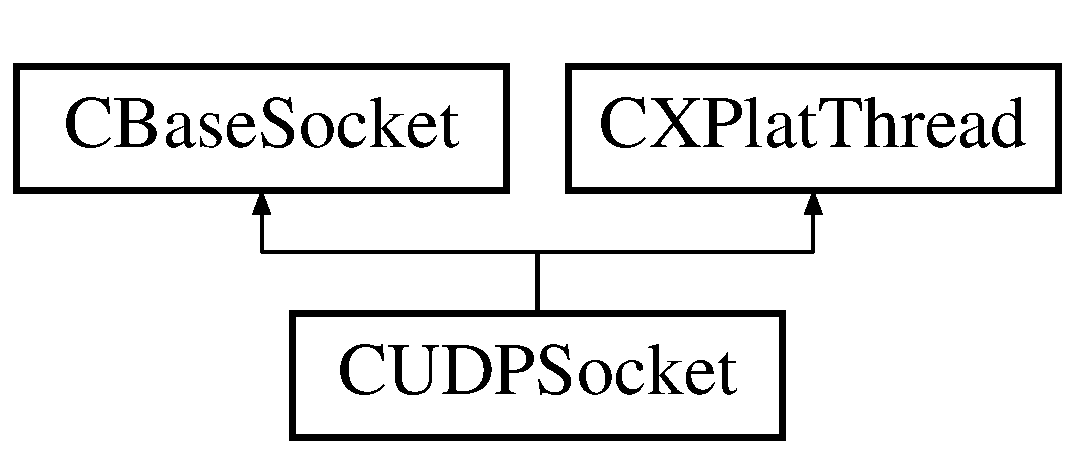
\includegraphics[height=2.000000cm]{class_c_u_d_p_socket}
\end{center}
\end{figure}
\subsection*{\-Public \-Types}
\begin{DoxyCompactItemize}
\item 
enum \{ \hyperlink{class_c_u_d_p_socket_a47208bbacf51eb5dcf13676e275b74faac90ae17c9b44fb66c6dd1c532e67c1e0}{\-D\-A\-T\-A\-\_\-\-B\-U\-F\-F\-E\-R\-\_\-\-S\-I\-Z\-E} =  0x800
 \}
\end{DoxyCompactItemize}
\subsection*{\-Public \-Member \-Functions}
\begin{DoxyCompactItemize}
\item 
\hyperlink{class_c_u_d_p_socket_aef5d2a06cf56ee8887f320e60078a82a}{\-C\-U\-D\-P\-Socket} ()
\item 
virtual \hyperlink{class_c_u_d_p_socket_a39013172842e53b7ea8ab7c4b6a9db34}{$\sim$\-C\-U\-D\-P\-Socket} ()
\item 
virtual \hyperlink{_cpclient_8h_a3be13892ae7076009afcf121347dd319}{\-B\-O\-O\-L} \hyperlink{class_c_u_d_p_socket_a6c89fafe2db1d38396deb319b753e429}{\-Create} (\hyperlink{_x_plat_8h_a45c20c14d3d8790a22153d08ab2eb2ff}{\-U\-I\-N\-T} n\-Port=0, \hyperlink{_x_plat_8h_a2b72c6037793f6c6381a09c83f27569b}{\-L\-P\-C\-S\-T\-R} lp\-Addr=\-N\-U\-L\-L, \hyperlink{_cpclient_8h_a3be13892ae7076009afcf121347dd319}{\-B\-O\-O\-L} b\-Reuse=\hyperlink{_x_plat_8h_aa8cecfc5c5c054d2875c03e77b7be15d}{\-T\-R\-U\-E}, \hyperlink{_cpclient_8h_a3be13892ae7076009afcf121347dd319}{\-B\-O\-O\-L} b\-Bind=\hyperlink{_x_plat_8h_aa8cecfc5c5c054d2875c03e77b7be15d}{\-T\-R\-U\-E})
\item 
virtual int \hyperlink{class_c_u_d_p_socket_aa2aae315397cc5b53080ca816f148729}{\-Send\-Msg} (unsigned char $\ast$lp\-Data, int i\-Length, char $\ast$p\-I\-P\-Address, int i\-Port)
\begin{DoxyCompactList}\small\item\em \-Default to bind the socket. \end{DoxyCompactList}\item 
virtual \hyperlink{_cpclient_8h_a6464f7480a0fd0ee170cba12b2c0497f}{void} \hyperlink{class_c_u_d_p_socket_a175b7da28268a52de47ec103775e77aa}{\-Set\-Broadcast\-Mode} (\hyperlink{_cpclient_8h_a3be13892ae7076009afcf121347dd319}{\-B\-O\-O\-L} b\-On=\hyperlink{_x_plat_8h_aa8cecfc5c5c054d2875c03e77b7be15d}{\-T\-R\-U\-E})
\item 
virtual \hyperlink{_cpclient_8h_a6464f7480a0fd0ee170cba12b2c0497f}{void} \hyperlink{class_c_u_d_p_socket_a4c3f6638dc3c4cbe3ea33ab8b1dd811c}{\-Close\-Socket} ()
\begin{DoxyCompactList}\small\item\em \-Close socket. \end{DoxyCompactList}\item 
\hyperlink{_cpclient_8h_a6464f7480a0fd0ee170cba12b2c0497f}{void} \hyperlink{class_c_u_d_p_socket_aa48bf25adb1041c5f616fe5687607f6f}{\-Stop\-Thread} ()
\end{DoxyCompactItemize}
\subsection*{\-Protected \-Member \-Functions}
\begin{DoxyCompactItemize}
\item 
virtual unsigned \hyperlink{class_c_u_d_p_socket_ab33c06fd2594ab658f8addbb1a4944aa}{\-Worker\-Function} (\hyperlink{_cpclient_8h_a6464f7480a0fd0ee170cba12b2c0497f}{void} $\ast$p\-Param)
\begin{DoxyCompactList}\small\item\em \-Called by \hyperlink{class_c_x_plat_thread}{\-C\-X\-Plat\-Thread} to start work in object context. \end{DoxyCompactList}\item 
virtual int \hyperlink{class_c_u_d_p_socket_a6e809eadb40d97b4991f3e6b21fd3b87}{\-Handle\-Receive\-Data} ()
\item 
virtual \hyperlink{_cpclient_8h_a6464f7480a0fd0ee170cba12b2c0497f}{void} \hyperlink{class_c_u_d_p_socket_ab31aee7d247dad588476c2203ad84d18}{\-Process\-Data} (unsigned char $\ast$lp\-Data, int i\-Length, struct sockaddr\-\_\-in $\ast$addr\-From)=0
\begin{DoxyCompactList}\small\item\em call back to receive data \end{DoxyCompactList}\end{DoxyCompactItemize}
\subsection*{\-Static \-Protected \-Member \-Functions}
\begin{DoxyCompactItemize}
\item 
static unsigned \hyperlink{_x_plat_8h_a3107b1d0ca10d4ae4575d9107d4cbffe}{\-\_\-stdcall} \hyperlink{class_c_u_d_p_socket_a62fafcc570b0df054ad766171cd976bd}{\-Receive\-Data\-Thread} (\hyperlink{_cpclient_8h_a6464f7480a0fd0ee170cba12b2c0497f}{void} $\ast$p\-Void)
\end{DoxyCompactItemize}
\subsection*{\-Protected \-Attributes}
\begin{DoxyCompactItemize}
\item 
\hyperlink{class_c_x_plat_event}{\-C\-X\-Plat\-Event} \hyperlink{class_c_u_d_p_socket_abded5c32659597c7090dba34bbf3320f}{c\-Stop\-Event}
\begin{DoxyCompactList}\small\item\em pure virturl, process received data \end{DoxyCompactList}\item 
unsigned char \hyperlink{class_c_u_d_p_socket_adba8b62f17aa86ca7d6dc7514a998d8b}{uc\-Buffer} \mbox{[}\hyperlink{class_c_u_d_p_socket_a47208bbacf51eb5dcf13676e275b74faac90ae17c9b44fb66c6dd1c532e67c1e0}{\-D\-A\-T\-A\-\_\-\-B\-U\-F\-F\-E\-R\-\_\-\-S\-I\-Z\-E}\mbox{]}
\end{DoxyCompactItemize}


\subsection{\-Detailed \-Description}
\hyperlink{_c_u_d_p_socket_8h}{\-C\-U\-D\-P\-Socket.\-h}\-: interface for the \hyperlink{class_c_u_d_p_socket}{\-C\-U\-D\-P\-Socket} class. 

\-\_\-\-M\-S\-C\-\_\-\-V\-E\-R $>$ 1000 \-U\-D\-P socket class 

\-Definition at line 33 of file \-C\-U\-D\-P\-Socket.\-h.



\subsection{\-Member \-Enumeration \-Documentation}
\hypertarget{class_c_u_d_p_socket_a47208bbacf51eb5dcf13676e275b74fa}{\subsubsection[{anonymous enum}]{\setlength{\rightskip}{0pt plus 5cm}anonymous enum}}\label{class_c_u_d_p_socket_a47208bbacf51eb5dcf13676e275b74fa}
\begin{Desc}
\item[\-Enumerator\-: ]\par
\begin{description}
\index{\-D\-A\-T\-A\-\_\-\-B\-U\-F\-F\-E\-R\-\_\-\-S\-I\-Z\-E@{\-D\-A\-T\-A\-\_\-\-B\-U\-F\-F\-E\-R\-\_\-\-S\-I\-Z\-E}!\-C\-U\-D\-P\-Socket@{\-C\-U\-D\-P\-Socket}}\index{\-C\-U\-D\-P\-Socket@{\-C\-U\-D\-P\-Socket}!\-D\-A\-T\-A\-\_\-\-B\-U\-F\-F\-E\-R\-\_\-\-S\-I\-Z\-E@{\-D\-A\-T\-A\-\_\-\-B\-U\-F\-F\-E\-R\-\_\-\-S\-I\-Z\-E}}\item[{\em 
\hypertarget{class_c_u_d_p_socket_a47208bbacf51eb5dcf13676e275b74faac90ae17c9b44fb66c6dd1c532e67c1e0}{\-D\-A\-T\-A\-\_\-\-B\-U\-F\-F\-E\-R\-\_\-\-S\-I\-Z\-E}\label{class_c_u_d_p_socket_a47208bbacf51eb5dcf13676e275b74faac90ae17c9b44fb66c6dd1c532e67c1e0}
}]\end{description}
\end{Desc}



\-Definition at line 47 of file \-C\-U\-D\-P\-Socket.\-h.



\subsection{\-Constructor \& \-Destructor \-Documentation}
\hypertarget{class_c_u_d_p_socket_aef5d2a06cf56ee8887f320e60078a82a}{\index{\-C\-U\-D\-P\-Socket@{\-C\-U\-D\-P\-Socket}!\-C\-U\-D\-P\-Socket@{\-C\-U\-D\-P\-Socket}}
\index{\-C\-U\-D\-P\-Socket@{\-C\-U\-D\-P\-Socket}!CUDPSocket@{\-C\-U\-D\-P\-Socket}}
\subsubsection[{\-C\-U\-D\-P\-Socket}]{\setlength{\rightskip}{0pt plus 5cm}{\bf \-C\-U\-D\-P\-Socket\-::\-C\-U\-D\-P\-Socket} (
\begin{DoxyParamCaption}
{}
\end{DoxyParamCaption}
)}}\label{class_c_u_d_p_socket_aef5d2a06cf56ee8887f320e60078a82a}


\-Definition at line 26 of file \-C\-U\-D\-P\-Socket.\-cpp.

\hypertarget{class_c_u_d_p_socket_a39013172842e53b7ea8ab7c4b6a9db34}{\index{\-C\-U\-D\-P\-Socket@{\-C\-U\-D\-P\-Socket}!$\sim$\-C\-U\-D\-P\-Socket@{$\sim$\-C\-U\-D\-P\-Socket}}
\index{$\sim$\-C\-U\-D\-P\-Socket@{$\sim$\-C\-U\-D\-P\-Socket}!CUDPSocket@{\-C\-U\-D\-P\-Socket}}
\subsubsection[{$\sim$\-C\-U\-D\-P\-Socket}]{\setlength{\rightskip}{0pt plus 5cm}{\bf \-C\-U\-D\-P\-Socket\-::$\sim$\-C\-U\-D\-P\-Socket} (
\begin{DoxyParamCaption}
{}
\end{DoxyParamCaption}
)\hspace{0.3cm}{\ttfamily  \mbox{[}virtual\mbox{]}}}}\label{class_c_u_d_p_socket_a39013172842e53b7ea8ab7c4b6a9db34}


\-Definition at line 30 of file \-C\-U\-D\-P\-Socket.\-cpp.



\subsection{\-Member \-Function \-Documentation}
\hypertarget{class_c_u_d_p_socket_a4c3f6638dc3c4cbe3ea33ab8b1dd811c}{\index{\-C\-U\-D\-P\-Socket@{\-C\-U\-D\-P\-Socket}!\-Close\-Socket@{\-Close\-Socket}}
\index{\-Close\-Socket@{\-Close\-Socket}!CUDPSocket@{\-C\-U\-D\-P\-Socket}}
\subsubsection[{\-Close\-Socket}]{\setlength{\rightskip}{0pt plus 5cm}{\bf void} {\bf \-C\-U\-D\-P\-Socket\-::\-Close\-Socket} (
\begin{DoxyParamCaption}
{}
\end{DoxyParamCaption}
)\hspace{0.3cm}{\ttfamily  \mbox{[}virtual\mbox{]}}}}\label{class_c_u_d_p_socket_a4c3f6638dc3c4cbe3ea33ab8b1dd811c}


\-Close socket. 



\-Reimplemented from \hyperlink{class_c_base_socket_ad1e45ab8be1fda6f91704a7159a0a8e4}{\-C\-Base\-Socket}.



\-Definition at line 173 of file \-C\-U\-D\-P\-Socket.\-cpp.

\hypertarget{class_c_u_d_p_socket_a6c89fafe2db1d38396deb319b753e429}{\index{\-C\-U\-D\-P\-Socket@{\-C\-U\-D\-P\-Socket}!\-Create@{\-Create}}
\index{\-Create@{\-Create}!CUDPSocket@{\-C\-U\-D\-P\-Socket}}
\subsubsection[{\-Create}]{\setlength{\rightskip}{0pt plus 5cm}{\bf \-B\-O\-O\-L} {\bf \-C\-U\-D\-P\-Socket\-::\-Create} (
\begin{DoxyParamCaption}
\item[{{\bf \-U\-I\-N\-T}}]{n\-Port = {\ttfamily 0}, }
\item[{{\bf \-L\-P\-C\-S\-T\-R}}]{lp\-Addr = {\ttfamily \-N\-U\-L\-L}, }
\item[{{\bf \-B\-O\-O\-L}}]{b\-Reuse = {\ttfamily {\bf \-T\-R\-U\-E}}, }
\item[{{\bf \-B\-O\-O\-L}}]{b\-Bind = {\ttfamily {\bf \-T\-R\-U\-E}}}
\end{DoxyParamCaption}
)\hspace{0.3cm}{\ttfamily  \mbox{[}virtual\mbox{]}}}}\label{class_c_u_d_p_socket_a6c89fafe2db1d38396deb319b753e429}

\begin{DoxyParams}{\-Parameters}
{\em lp\-Addr} & \-Port \\
\hline
{\em b\-Reuse} & \-Inet address in the standard xxx.\-xxx.\-xxx.\-xxx format \\
\hline
{\em b\-Bind} & \-Allow reuse of this socket \\
\hline
\end{DoxyParams}


\-Definition at line 35 of file \-C\-U\-D\-P\-Socket.\-cpp.

\hypertarget{class_c_u_d_p_socket_a6e809eadb40d97b4991f3e6b21fd3b87}{\index{\-C\-U\-D\-P\-Socket@{\-C\-U\-D\-P\-Socket}!\-Handle\-Receive\-Data@{\-Handle\-Receive\-Data}}
\index{\-Handle\-Receive\-Data@{\-Handle\-Receive\-Data}!CUDPSocket@{\-C\-U\-D\-P\-Socket}}
\subsubsection[{\-Handle\-Receive\-Data}]{\setlength{\rightskip}{0pt plus 5cm}int {\bf \-C\-U\-D\-P\-Socket\-::\-Handle\-Receive\-Data} (
\begin{DoxyParamCaption}
{}
\end{DoxyParamCaption}
)\hspace{0.3cm}{\ttfamily  \mbox{[}protected, virtual\mbox{]}}}}\label{class_c_u_d_p_socket_a6e809eadb40d97b4991f3e6b21fd3b87}


\-Definition at line 65 of file \-C\-U\-D\-P\-Socket.\-cpp.

\hypertarget{class_c_u_d_p_socket_ab31aee7d247dad588476c2203ad84d18}{\index{\-C\-U\-D\-P\-Socket@{\-C\-U\-D\-P\-Socket}!\-Process\-Data@{\-Process\-Data}}
\index{\-Process\-Data@{\-Process\-Data}!CUDPSocket@{\-C\-U\-D\-P\-Socket}}
\subsubsection[{\-Process\-Data}]{\setlength{\rightskip}{0pt plus 5cm}virtual {\bf void} {\bf \-C\-U\-D\-P\-Socket\-::\-Process\-Data} (
\begin{DoxyParamCaption}
\item[{unsigned char $\ast$}]{lp\-Data, }
\item[{int}]{i\-Length, }
\item[{struct sockaddr\-\_\-in $\ast$}]{addr\-From}
\end{DoxyParamCaption}
)\hspace{0.3cm}{\ttfamily  \mbox{[}protected, pure virtual\mbox{]}}}}\label{class_c_u_d_p_socket_ab31aee7d247dad588476c2203ad84d18}


call back to receive data 

\hypertarget{class_c_u_d_p_socket_a62fafcc570b0df054ad766171cd976bd}{\index{\-C\-U\-D\-P\-Socket@{\-C\-U\-D\-P\-Socket}!\-Receive\-Data\-Thread@{\-Receive\-Data\-Thread}}
\index{\-Receive\-Data\-Thread@{\-Receive\-Data\-Thread}!CUDPSocket@{\-C\-U\-D\-P\-Socket}}
\subsubsection[{\-Receive\-Data\-Thread}]{\setlength{\rightskip}{0pt plus 5cm}static unsigned {\bf \-\_\-stdcall} {\bf \-C\-U\-D\-P\-Socket\-::\-Receive\-Data\-Thread} (
\begin{DoxyParamCaption}
\item[{{\bf void} $\ast$}]{p\-Void}
\end{DoxyParamCaption}
)\hspace{0.3cm}{\ttfamily  \mbox{[}static, protected\mbox{]}}}}\label{class_c_u_d_p_socket_a62fafcc570b0df054ad766171cd976bd}
\hypertarget{class_c_u_d_p_socket_aa2aae315397cc5b53080ca816f148729}{\index{\-C\-U\-D\-P\-Socket@{\-C\-U\-D\-P\-Socket}!\-Send\-Msg@{\-Send\-Msg}}
\index{\-Send\-Msg@{\-Send\-Msg}!CUDPSocket@{\-C\-U\-D\-P\-Socket}}
\subsubsection[{\-Send\-Msg}]{\setlength{\rightskip}{0pt plus 5cm}int {\bf \-C\-U\-D\-P\-Socket\-::\-Send\-Msg} (
\begin{DoxyParamCaption}
\item[{unsigned char $\ast$}]{lp\-Data, }
\item[{int}]{i\-Length, }
\item[{char $\ast$}]{p\-I\-P\-Address, }
\item[{int}]{i\-Port}
\end{DoxyParamCaption}
)\hspace{0.3cm}{\ttfamily  \mbox{[}virtual\mbox{]}}}}\label{class_c_u_d_p_socket_aa2aae315397cc5b53080ca816f148729}


\-Default to bind the socket. 



\-Definition at line 142 of file \-C\-U\-D\-P\-Socket.\-cpp.

\hypertarget{class_c_u_d_p_socket_a175b7da28268a52de47ec103775e77aa}{\index{\-C\-U\-D\-P\-Socket@{\-C\-U\-D\-P\-Socket}!\-Set\-Broadcast\-Mode@{\-Set\-Broadcast\-Mode}}
\index{\-Set\-Broadcast\-Mode@{\-Set\-Broadcast\-Mode}!CUDPSocket@{\-C\-U\-D\-P\-Socket}}
\subsubsection[{\-Set\-Broadcast\-Mode}]{\setlength{\rightskip}{0pt plus 5cm}{\bf void} {\bf \-C\-U\-D\-P\-Socket\-::\-Set\-Broadcast\-Mode} (
\begin{DoxyParamCaption}
\item[{{\bf \-B\-O\-O\-L}}]{b\-On = {\ttfamily {\bf \-T\-R\-U\-E}}}
\end{DoxyParamCaption}
)\hspace{0.3cm}{\ttfamily  \mbox{[}virtual\mbox{]}}}}\label{class_c_u_d_p_socket_a175b7da28268a52de47ec103775e77aa}


\-Definition at line 188 of file \-C\-U\-D\-P\-Socket.\-cpp.

\hypertarget{class_c_u_d_p_socket_aa48bf25adb1041c5f616fe5687607f6f}{\index{\-C\-U\-D\-P\-Socket@{\-C\-U\-D\-P\-Socket}!\-Stop\-Thread@{\-Stop\-Thread}}
\index{\-Stop\-Thread@{\-Stop\-Thread}!CUDPSocket@{\-C\-U\-D\-P\-Socket}}
\subsubsection[{\-Stop\-Thread}]{\setlength{\rightskip}{0pt plus 5cm}{\bf void} {\bf \-C\-U\-D\-P\-Socket\-::\-Stop\-Thread} (
\begin{DoxyParamCaption}
{}
\end{DoxyParamCaption}
)}}\label{class_c_u_d_p_socket_aa48bf25adb1041c5f616fe5687607f6f}


\-Definition at line 179 of file \-C\-U\-D\-P\-Socket.\-cpp.

\hypertarget{class_c_u_d_p_socket_ab33c06fd2594ab658f8addbb1a4944aa}{\index{\-C\-U\-D\-P\-Socket@{\-C\-U\-D\-P\-Socket}!\-Worker\-Function@{\-Worker\-Function}}
\index{\-Worker\-Function@{\-Worker\-Function}!CUDPSocket@{\-C\-U\-D\-P\-Socket}}
\subsubsection[{\-Worker\-Function}]{\setlength{\rightskip}{0pt plus 5cm}unsigned {\bf \-C\-U\-D\-P\-Socket\-::\-Worker\-Function} (
\begin{DoxyParamCaption}
\item[{{\bf void} $\ast$}]{p\-Param}
\end{DoxyParamCaption}
)\hspace{0.3cm}{\ttfamily  \mbox{[}protected, virtual\mbox{]}}}}\label{class_c_u_d_p_socket_ab33c06fd2594ab658f8addbb1a4944aa}


\-Called by \hyperlink{class_c_x_plat_thread}{\-C\-X\-Plat\-Thread} to start work in object context. 



\-Implements \hyperlink{class_c_x_plat_thread_af8a15900817f9673c6fd8e85cdedf27d}{\-C\-X\-Plat\-Thread}.



\-Definition at line 44 of file \-C\-U\-D\-P\-Socket.\-cpp.



\subsection{\-Member \-Data \-Documentation}
\hypertarget{class_c_u_d_p_socket_abded5c32659597c7090dba34bbf3320f}{\index{\-C\-U\-D\-P\-Socket@{\-C\-U\-D\-P\-Socket}!c\-Stop\-Event@{c\-Stop\-Event}}
\index{c\-Stop\-Event@{c\-Stop\-Event}!CUDPSocket@{\-C\-U\-D\-P\-Socket}}
\subsubsection[{c\-Stop\-Event}]{\setlength{\rightskip}{0pt plus 5cm}{\bf \-C\-X\-Plat\-Event} {\bf \-C\-U\-D\-P\-Socket\-::c\-Stop\-Event}\hspace{0.3cm}{\ttfamily  \mbox{[}protected\mbox{]}}}}\label{class_c_u_d_p_socket_abded5c32659597c7090dba34bbf3320f}


pure virturl, process received data 



\-Definition at line 57 of file \-C\-U\-D\-P\-Socket.\-h.

\hypertarget{class_c_u_d_p_socket_adba8b62f17aa86ca7d6dc7514a998d8b}{\index{\-C\-U\-D\-P\-Socket@{\-C\-U\-D\-P\-Socket}!uc\-Buffer@{uc\-Buffer}}
\index{uc\-Buffer@{uc\-Buffer}!CUDPSocket@{\-C\-U\-D\-P\-Socket}}
\subsubsection[{uc\-Buffer}]{\setlength{\rightskip}{0pt plus 5cm}unsigned char {\bf \-C\-U\-D\-P\-Socket\-::uc\-Buffer}\mbox{[}{\bf \-D\-A\-T\-A\-\_\-\-B\-U\-F\-F\-E\-R\-\_\-\-S\-I\-Z\-E}\mbox{]}\hspace{0.3cm}{\ttfamily  \mbox{[}protected\mbox{]}}}}\label{class_c_u_d_p_socket_adba8b62f17aa86ca7d6dc7514a998d8b}


\-Definition at line 58 of file \-C\-U\-D\-P\-Socket.\-h.



\-The documentation for this class was generated from the following files\-:\begin{DoxyCompactItemize}
\item 
common/\hyperlink{_c_u_d_p_socket_8h}{\-C\-U\-D\-P\-Socket.\-h}\item 
common/\hyperlink{_c_u_d_p_socket_8cpp}{\-C\-U\-D\-P\-Socket.\-cpp}\end{DoxyCompactItemize}

\hypertarget{class_c_x_plat_critical_section}{\section{\-C\-X\-Plat\-Critical\-Section \-Class \-Reference}
\label{class_c_x_plat_critical_section}\index{\-C\-X\-Plat\-Critical\-Section@{\-C\-X\-Plat\-Critical\-Section}}
}


{\ttfamily \#include $<$\-C\-X\-Plat\-Critical\-Section.\-h$>$}

\subsection*{\-Public \-Member \-Functions}
\begin{DoxyCompactItemize}
\item 
\hyperlink{class_c_x_plat_critical_section_a8188427bafd98f8778ecfbac5e4d962e}{\-C\-X\-Plat\-Critical\-Section} ()
\begin{DoxyCompactList}\small\item\em \-Constructor. \end{DoxyCompactList}\item 
\hyperlink{class_c_x_plat_critical_section_a17fee86e9af86ff7f2d922a77779651a}{$\sim$\-C\-X\-Plat\-Critical\-Section} ()
\begin{DoxyCompactList}\small\item\em \-Destructor. \end{DoxyCompactList}\item 
int \hyperlink{class_c_x_plat_critical_section_a09abc6317892511112edf7b8978ef670}{\-Lock} (\hyperlink{_x_plat_8h_aa39b39d94407451a6ec0226479db68cf}{\-D\-W\-O\-R\-D} dw\-Wait=\hyperlink{_x_plat_8h_aa84a29002ab81c719c0d07bb446296e0}{\-I\-N\-F\-I\-N\-I\-T\-E})
\begin{DoxyCompactList}\small\item\em \-Tries to obtain exclusive access. \end{DoxyCompactList}\item 
int \hyperlink{class_c_x_plat_critical_section_abc3ddf88e89230c7c97e98af9bd7c707}{\-Unlock} ()
\begin{DoxyCompactList}\small\item\em \-Releases exclusive access. \end{DoxyCompactList}\end{DoxyCompactItemize}
\subsection*{\-Protected \-Attributes}
\begin{DoxyCompactItemize}
\item 
pthread\-\_\-mutex\-\_\-t \hyperlink{class_c_x_plat_critical_section_aa7bacade5b04643e1a50122a0ba38fc5}{m\-\_\-cs\-Handle}
\item 
pthread\-\_\-t \hyperlink{class_c_x_plat_critical_section_a90276ecb4828f7c51166fc6588e31d22}{lock\-\_\-id}
\item 
int \hyperlink{class_c_x_plat_critical_section_a0bc1b3ef29deaac5438dd6ab245c0b9d}{lock\-\_\-count}
\end{DoxyCompactItemize}
\subsection*{\-Friends}
\begin{DoxyCompactItemize}
\item 
class \hyperlink{class_c_x_plat_critical_section_a07b9fb7f9e1f7c3e3f6604a7cc379be1}{\-C\-X\-Plat\-Event}
\end{DoxyCompactItemize}


\subsection{\-Detailed \-Description}
\-Cross plaform synchronization class

\-On \-Windows, critical sections are \char`\"{}cheaper\char`\"{} than interprocess mutexes (mutii?) 

\-Definition at line 26 of file \-C\-X\-Plat\-Critical\-Section.\-h.



\subsection{\-Constructor \& \-Destructor \-Documentation}
\hypertarget{class_c_x_plat_critical_section_a8188427bafd98f8778ecfbac5e4d962e}{\index{\-C\-X\-Plat\-Critical\-Section@{\-C\-X\-Plat\-Critical\-Section}!\-C\-X\-Plat\-Critical\-Section@{\-C\-X\-Plat\-Critical\-Section}}
\index{\-C\-X\-Plat\-Critical\-Section@{\-C\-X\-Plat\-Critical\-Section}!CXPlatCriticalSection@{\-C\-X\-Plat\-Critical\-Section}}
\subsubsection[{\-C\-X\-Plat\-Critical\-Section}]{\setlength{\rightskip}{0pt plus 5cm}{\bf \-C\-X\-Plat\-Critical\-Section\-::\-C\-X\-Plat\-Critical\-Section} (
\begin{DoxyParamCaption}
{}
\end{DoxyParamCaption}
)}}\label{class_c_x_plat_critical_section_a8188427bafd98f8778ecfbac5e4d962e}


\-Constructor. 



\-Definition at line 26 of file \-C\-X\-Plat\-Critical\-Section.\-cpp.

\hypertarget{class_c_x_plat_critical_section_a17fee86e9af86ff7f2d922a77779651a}{\index{\-C\-X\-Plat\-Critical\-Section@{\-C\-X\-Plat\-Critical\-Section}!$\sim$\-C\-X\-Plat\-Critical\-Section@{$\sim$\-C\-X\-Plat\-Critical\-Section}}
\index{$\sim$\-C\-X\-Plat\-Critical\-Section@{$\sim$\-C\-X\-Plat\-Critical\-Section}!CXPlatCriticalSection@{\-C\-X\-Plat\-Critical\-Section}}
\subsubsection[{$\sim$\-C\-X\-Plat\-Critical\-Section}]{\setlength{\rightskip}{0pt plus 5cm}{\bf \-C\-X\-Plat\-Critical\-Section\-::$\sim$\-C\-X\-Plat\-Critical\-Section} (
\begin{DoxyParamCaption}
{}
\end{DoxyParamCaption}
)}}\label{class_c_x_plat_critical_section_a17fee86e9af86ff7f2d922a77779651a}


\-Destructor. 



\-Definition at line 38 of file \-C\-X\-Plat\-Critical\-Section.\-cpp.



\subsection{\-Member \-Function \-Documentation}
\hypertarget{class_c_x_plat_critical_section_a09abc6317892511112edf7b8978ef670}{\index{\-C\-X\-Plat\-Critical\-Section@{\-C\-X\-Plat\-Critical\-Section}!\-Lock@{\-Lock}}
\index{\-Lock@{\-Lock}!CXPlatCriticalSection@{\-C\-X\-Plat\-Critical\-Section}}
\subsubsection[{\-Lock}]{\setlength{\rightskip}{0pt plus 5cm}int {\bf \-C\-X\-Plat\-Critical\-Section\-::\-Lock} (
\begin{DoxyParamCaption}
\item[{{\bf \-D\-W\-O\-R\-D}}]{dw\-Wait = {\ttfamily {\bf \-I\-N\-F\-I\-N\-I\-T\-E}}}
\end{DoxyParamCaption}
)}}\label{class_c_x_plat_critical_section_a09abc6317892511112edf7b8978ef670}


\-Tries to obtain exclusive access. 



\-Definition at line 49 of file \-C\-X\-Plat\-Critical\-Section.\-cpp.

\hypertarget{class_c_x_plat_critical_section_abc3ddf88e89230c7c97e98af9bd7c707}{\index{\-C\-X\-Plat\-Critical\-Section@{\-C\-X\-Plat\-Critical\-Section}!\-Unlock@{\-Unlock}}
\index{\-Unlock@{\-Unlock}!CXPlatCriticalSection@{\-C\-X\-Plat\-Critical\-Section}}
\subsubsection[{\-Unlock}]{\setlength{\rightskip}{0pt plus 5cm}int {\bf \-C\-X\-Plat\-Critical\-Section\-::\-Unlock} (
\begin{DoxyParamCaption}
{}
\end{DoxyParamCaption}
)}}\label{class_c_x_plat_critical_section_abc3ddf88e89230c7c97e98af9bd7c707}


\-Releases exclusive access. 



\-Definition at line 88 of file \-C\-X\-Plat\-Critical\-Section.\-cpp.



\subsection{\-Friends \-And \-Related \-Function \-Documentation}
\hypertarget{class_c_x_plat_critical_section_a07b9fb7f9e1f7c3e3f6604a7cc379be1}{\index{\-C\-X\-Plat\-Critical\-Section@{\-C\-X\-Plat\-Critical\-Section}!\-C\-X\-Plat\-Event@{\-C\-X\-Plat\-Event}}
\index{\-C\-X\-Plat\-Event@{\-C\-X\-Plat\-Event}!CXPlatCriticalSection@{\-C\-X\-Plat\-Critical\-Section}}
\subsubsection[{\-C\-X\-Plat\-Event}]{\setlength{\rightskip}{0pt plus 5cm}friend class {\bf \-C\-X\-Plat\-Event}\hspace{0.3cm}{\ttfamily  \mbox{[}friend\mbox{]}}}}\label{class_c_x_plat_critical_section_a07b9fb7f9e1f7c3e3f6604a7cc379be1}


\-Definition at line 28 of file \-C\-X\-Plat\-Critical\-Section.\-h.



\subsection{\-Member \-Data \-Documentation}
\hypertarget{class_c_x_plat_critical_section_a0bc1b3ef29deaac5438dd6ab245c0b9d}{\index{\-C\-X\-Plat\-Critical\-Section@{\-C\-X\-Plat\-Critical\-Section}!lock\-\_\-count@{lock\-\_\-count}}
\index{lock\-\_\-count@{lock\-\_\-count}!CXPlatCriticalSection@{\-C\-X\-Plat\-Critical\-Section}}
\subsubsection[{lock\-\_\-count}]{\setlength{\rightskip}{0pt plus 5cm}int {\bf \-C\-X\-Plat\-Critical\-Section\-::lock\-\_\-count}\hspace{0.3cm}{\ttfamily  \mbox{[}protected\mbox{]}}}}\label{class_c_x_plat_critical_section_a0bc1b3ef29deaac5438dd6ab245c0b9d}


\-Definition at line 46 of file \-C\-X\-Plat\-Critical\-Section.\-h.

\hypertarget{class_c_x_plat_critical_section_a90276ecb4828f7c51166fc6588e31d22}{\index{\-C\-X\-Plat\-Critical\-Section@{\-C\-X\-Plat\-Critical\-Section}!lock\-\_\-id@{lock\-\_\-id}}
\index{lock\-\_\-id@{lock\-\_\-id}!CXPlatCriticalSection@{\-C\-X\-Plat\-Critical\-Section}}
\subsubsection[{lock\-\_\-id}]{\setlength{\rightskip}{0pt plus 5cm}pthread\-\_\-t {\bf \-C\-X\-Plat\-Critical\-Section\-::lock\-\_\-id}\hspace{0.3cm}{\ttfamily  \mbox{[}protected\mbox{]}}}}\label{class_c_x_plat_critical_section_a90276ecb4828f7c51166fc6588e31d22}


\-Definition at line 45 of file \-C\-X\-Plat\-Critical\-Section.\-h.

\hypertarget{class_c_x_plat_critical_section_aa7bacade5b04643e1a50122a0ba38fc5}{\index{\-C\-X\-Plat\-Critical\-Section@{\-C\-X\-Plat\-Critical\-Section}!m\-\_\-cs\-Handle@{m\-\_\-cs\-Handle}}
\index{m\-\_\-cs\-Handle@{m\-\_\-cs\-Handle}!CXPlatCriticalSection@{\-C\-X\-Plat\-Critical\-Section}}
\subsubsection[{m\-\_\-cs\-Handle}]{\setlength{\rightskip}{0pt plus 5cm}pthread\-\_\-mutex\-\_\-t {\bf \-C\-X\-Plat\-Critical\-Section\-::m\-\_\-cs\-Handle}\hspace{0.3cm}{\ttfamily  \mbox{[}protected\mbox{]}}}}\label{class_c_x_plat_critical_section_aa7bacade5b04643e1a50122a0ba38fc5}


\-Definition at line 44 of file \-C\-X\-Plat\-Critical\-Section.\-h.



\-The documentation for this class was generated from the following files\-:\begin{DoxyCompactItemize}
\item 
common/\hyperlink{_c_x_plat_critical_section_8h}{\-C\-X\-Plat\-Critical\-Section.\-h}\item 
common/\hyperlink{_c_x_plat_critical_section_8cpp}{\-C\-X\-Plat\-Critical\-Section.\-cpp}\end{DoxyCompactItemize}

\hypertarget{class_c_x_plat_event}{\section{\-C\-X\-Plat\-Event \-Class \-Reference}
\label{class_c_x_plat_event}\index{\-C\-X\-Plat\-Event@{\-C\-X\-Plat\-Event}}
}


\-Cross platform event synchronization class.  




{\ttfamily \#include $<$\-C\-X\-Plat\-Event.\-h$>$}

\subsection*{\-Public \-Member \-Functions}
\begin{DoxyCompactItemize}
\item 
\hyperlink{class_c_x_plat_event_a818eb0ba93b14314d0a153bad8b9c9ec}{\-C\-X\-Plat\-Event} (\hyperlink{_cpclient_8h_a3be13892ae7076009afcf121347dd319}{\-B\-O\-O\-L} \hyperlink{class_c_x_plat_event_aa588099a688b7be58346f5b05d55eb91}{b\-Manual\-Reset}=\hyperlink{_x_plat_8h_aa93f0eb578d23995850d61f7d61c55c1}{\-F\-A\-L\-S\-E})
\begin{DoxyCompactList}\small\item\em \-Constructor. \end{DoxyCompactList}\item 
\hyperlink{class_c_x_plat_event_a448a4eee2fd5ac8e5a5e1550850bdbd9}{$\sim$\-C\-X\-Plat\-Event} ()
\begin{DoxyCompactList}\small\item\em \-Destructor. \end{DoxyCompactList}\item 
int \hyperlink{class_c_x_plat_event_ad053765292f1c8d1f91c730e805b8fa5}{\-Lock} (\hyperlink{_x_plat_8h_aa39b39d94407451a6ec0226479db68cf}{\-D\-W\-O\-R\-D} dw\-Wait=\hyperlink{_x_plat_8h_aa84a29002ab81c719c0d07bb446296e0}{\-I\-N\-F\-I\-N\-I\-T\-E})
\begin{DoxyCompactList}\small\item\em \-Tries to obtain access. \end{DoxyCompactList}\item 
\hyperlink{_cpclient_8h_a6464f7480a0fd0ee170cba12b2c0497f}{void} \hyperlink{class_c_x_plat_event_ad43844482b5cee3b03c6e38680b0a259}{\-Set\-Event} ()
\begin{DoxyCompactList}\small\item\em \-Set the event. \end{DoxyCompactList}\item 
\hyperlink{_cpclient_8h_a6464f7480a0fd0ee170cba12b2c0497f}{void} \hyperlink{class_c_x_plat_event_a1191adf0a0631aa8d0c8f78572b456be}{\-Reset\-Event} ()
\begin{DoxyCompactList}\small\item\em \-Reset event to non-\/signalled. \end{DoxyCompactList}\item 
\hyperlink{_cpclient_8h_a3be13892ae7076009afcf121347dd319}{\-B\-O\-O\-L} \hyperlink{class_c_x_plat_event_a252bc188f5077f656cbf2190dbd074b3}{\-Was\-Created\-Successfully} ()
\begin{DoxyCompactList}\small\item\em \-Was the event created successfully. \end{DoxyCompactList}\end{DoxyCompactItemize}
\subsection*{\-Protected \-Attributes}
\begin{DoxyCompactItemize}
\item 
\hyperlink{_cpclient_8h_a3be13892ae7076009afcf121347dd319}{\-B\-O\-O\-L} \hyperlink{class_c_x_plat_event_ace78909b8e610373b1ffb6fc4fde3ee6}{b\-Event\-Created}
\item 
\hyperlink{_cpclient_8h_a3be13892ae7076009afcf121347dd319}{\-B\-O\-O\-L} \hyperlink{class_c_x_plat_event_aa588099a688b7be58346f5b05d55eb91}{b\-Manual\-Reset}
\item 
pthread\-\_\-cond\-\_\-t \hyperlink{class_c_x_plat_event_ad452214355d4b5989c30ed1e7f137544}{m\-\_\-cs\-Handle}
\item 
sem\-\_\-t \hyperlink{class_c_x_plat_event_aebee3d1cc992443887951cd69642de35}{pt\-Sem}
\item 
int \hyperlink{class_c_x_plat_event_aad997af175335943b6eea0ba9f870df6}{i\-Set\-Count}
\end{DoxyCompactItemize}


\subsection{\-Detailed \-Description}
\-Cross platform event synchronization class. 

\-Definition at line 28 of file \-C\-X\-Plat\-Event.\-h.



\subsection{\-Constructor \& \-Destructor \-Documentation}
\hypertarget{class_c_x_plat_event_a818eb0ba93b14314d0a153bad8b9c9ec}{\index{\-C\-X\-Plat\-Event@{\-C\-X\-Plat\-Event}!\-C\-X\-Plat\-Event@{\-C\-X\-Plat\-Event}}
\index{\-C\-X\-Plat\-Event@{\-C\-X\-Plat\-Event}!CXPlatEvent@{\-C\-X\-Plat\-Event}}
\subsubsection[{\-C\-X\-Plat\-Event}]{\setlength{\rightskip}{0pt plus 5cm}{\bf \-C\-X\-Plat\-Event\-::\-C\-X\-Plat\-Event} (
\begin{DoxyParamCaption}
\item[{{\bf \-B\-O\-O\-L}}]{b\-Manual\-Reset = {\ttfamily {\bf \-F\-A\-L\-S\-E}}}
\end{DoxyParamCaption}
)}}\label{class_c_x_plat_event_a818eb0ba93b14314d0a153bad8b9c9ec}


\-Constructor. 



\-Definition at line 32 of file \-C\-X\-Plat\-Event.\-cpp.

\hypertarget{class_c_x_plat_event_a448a4eee2fd5ac8e5a5e1550850bdbd9}{\index{\-C\-X\-Plat\-Event@{\-C\-X\-Plat\-Event}!$\sim$\-C\-X\-Plat\-Event@{$\sim$\-C\-X\-Plat\-Event}}
\index{$\sim$\-C\-X\-Plat\-Event@{$\sim$\-C\-X\-Plat\-Event}!CXPlatEvent@{\-C\-X\-Plat\-Event}}
\subsubsection[{$\sim$\-C\-X\-Plat\-Event}]{\setlength{\rightskip}{0pt plus 5cm}{\bf \-C\-X\-Plat\-Event\-::$\sim$\-C\-X\-Plat\-Event} (
\begin{DoxyParamCaption}
{}
\end{DoxyParamCaption}
)}}\label{class_c_x_plat_event_a448a4eee2fd5ac8e5a5e1550850bdbd9}


\-Destructor. 

\-Cross platform mutex 

\-Definition at line 54 of file \-C\-X\-Plat\-Event.\-cpp.



\subsection{\-Member \-Function \-Documentation}
\hypertarget{class_c_x_plat_event_ad053765292f1c8d1f91c730e805b8fa5}{\index{\-C\-X\-Plat\-Event@{\-C\-X\-Plat\-Event}!\-Lock@{\-Lock}}
\index{\-Lock@{\-Lock}!CXPlatEvent@{\-C\-X\-Plat\-Event}}
\subsubsection[{\-Lock}]{\setlength{\rightskip}{0pt plus 5cm}int {\bf \-C\-X\-Plat\-Event\-::\-Lock} (
\begin{DoxyParamCaption}
\item[{{\bf \-D\-W\-O\-R\-D}}]{dw\-Wait = {\ttfamily {\bf \-I\-N\-F\-I\-N\-I\-T\-E}}}
\end{DoxyParamCaption}
)}}\label{class_c_x_plat_event_ad053765292f1c8d1f91c730e805b8fa5}


\-Tries to obtain access. 



\-Definition at line 92 of file \-C\-X\-Plat\-Event.\-cpp.

\hypertarget{class_c_x_plat_event_a1191adf0a0631aa8d0c8f78572b456be}{\index{\-C\-X\-Plat\-Event@{\-C\-X\-Plat\-Event}!\-Reset\-Event@{\-Reset\-Event}}
\index{\-Reset\-Event@{\-Reset\-Event}!CXPlatEvent@{\-C\-X\-Plat\-Event}}
\subsubsection[{\-Reset\-Event}]{\setlength{\rightskip}{0pt plus 5cm}{\bf void} {\bf \-C\-X\-Plat\-Event\-::\-Reset\-Event} (
\begin{DoxyParamCaption}
{}
\end{DoxyParamCaption}
)}}\label{class_c_x_plat_event_a1191adf0a0631aa8d0c8f78572b456be}


\-Reset event to non-\/signalled. 



\-Definition at line 70 of file \-C\-X\-Plat\-Event.\-cpp.

\hypertarget{class_c_x_plat_event_ad43844482b5cee3b03c6e38680b0a259}{\index{\-C\-X\-Plat\-Event@{\-C\-X\-Plat\-Event}!\-Set\-Event@{\-Set\-Event}}
\index{\-Set\-Event@{\-Set\-Event}!CXPlatEvent@{\-C\-X\-Plat\-Event}}
\subsubsection[{\-Set\-Event}]{\setlength{\rightskip}{0pt plus 5cm}{\bf void} {\bf \-C\-X\-Plat\-Event\-::\-Set\-Event} (
\begin{DoxyParamCaption}
{}
\end{DoxyParamCaption}
)}}\label{class_c_x_plat_event_ad43844482b5cee3b03c6e38680b0a259}


\-Set the event. 



\-Definition at line 121 of file \-C\-X\-Plat\-Event.\-cpp.

\hypertarget{class_c_x_plat_event_a252bc188f5077f656cbf2190dbd074b3}{\index{\-C\-X\-Plat\-Event@{\-C\-X\-Plat\-Event}!\-Was\-Created\-Successfully@{\-Was\-Created\-Successfully}}
\index{\-Was\-Created\-Successfully@{\-Was\-Created\-Successfully}!CXPlatEvent@{\-C\-X\-Plat\-Event}}
\subsubsection[{\-Was\-Created\-Successfully}]{\setlength{\rightskip}{0pt plus 5cm}{\bf \-B\-O\-O\-L} {\bf \-C\-X\-Plat\-Event\-::\-Was\-Created\-Successfully} (
\begin{DoxyParamCaption}
{}
\end{DoxyParamCaption}
)}}\label{class_c_x_plat_event_a252bc188f5077f656cbf2190dbd074b3}


\-Was the event created successfully. 



\-Definition at line 139 of file \-C\-X\-Plat\-Event.\-cpp.



\subsection{\-Member \-Data \-Documentation}
\hypertarget{class_c_x_plat_event_ace78909b8e610373b1ffb6fc4fde3ee6}{\index{\-C\-X\-Plat\-Event@{\-C\-X\-Plat\-Event}!b\-Event\-Created@{b\-Event\-Created}}
\index{b\-Event\-Created@{b\-Event\-Created}!CXPlatEvent@{\-C\-X\-Plat\-Event}}
\subsubsection[{b\-Event\-Created}]{\setlength{\rightskip}{0pt plus 5cm}{\bf \-B\-O\-O\-L} {\bf \-C\-X\-Plat\-Event\-::b\-Event\-Created}\hspace{0.3cm}{\ttfamily  \mbox{[}protected\mbox{]}}}}\label{class_c_x_plat_event_ace78909b8e610373b1ffb6fc4fde3ee6}


\-Definition at line 45 of file \-C\-X\-Plat\-Event.\-h.

\hypertarget{class_c_x_plat_event_aa588099a688b7be58346f5b05d55eb91}{\index{\-C\-X\-Plat\-Event@{\-C\-X\-Plat\-Event}!b\-Manual\-Reset@{b\-Manual\-Reset}}
\index{b\-Manual\-Reset@{b\-Manual\-Reset}!CXPlatEvent@{\-C\-X\-Plat\-Event}}
\subsubsection[{b\-Manual\-Reset}]{\setlength{\rightskip}{0pt plus 5cm}{\bf \-B\-O\-O\-L} {\bf \-C\-X\-Plat\-Event\-::b\-Manual\-Reset}\hspace{0.3cm}{\ttfamily  \mbox{[}protected\mbox{]}}}}\label{class_c_x_plat_event_aa588099a688b7be58346f5b05d55eb91}


\-Definition at line 46 of file \-C\-X\-Plat\-Event.\-h.

\hypertarget{class_c_x_plat_event_aad997af175335943b6eea0ba9f870df6}{\index{\-C\-X\-Plat\-Event@{\-C\-X\-Plat\-Event}!i\-Set\-Count@{i\-Set\-Count}}
\index{i\-Set\-Count@{i\-Set\-Count}!CXPlatEvent@{\-C\-X\-Plat\-Event}}
\subsubsection[{i\-Set\-Count}]{\setlength{\rightskip}{0pt plus 5cm}int {\bf \-C\-X\-Plat\-Event\-::i\-Set\-Count}\hspace{0.3cm}{\ttfamily  \mbox{[}protected\mbox{]}}}}\label{class_c_x_plat_event_aad997af175335943b6eea0ba9f870df6}


\-Definition at line 58 of file \-C\-X\-Plat\-Event.\-h.

\hypertarget{class_c_x_plat_event_ad452214355d4b5989c30ed1e7f137544}{\index{\-C\-X\-Plat\-Event@{\-C\-X\-Plat\-Event}!m\-\_\-cs\-Handle@{m\-\_\-cs\-Handle}}
\index{m\-\_\-cs\-Handle@{m\-\_\-cs\-Handle}!CXPlatEvent@{\-C\-X\-Plat\-Event}}
\subsubsection[{m\-\_\-cs\-Handle}]{\setlength{\rightskip}{0pt plus 5cm}pthread\-\_\-cond\-\_\-t {\bf \-C\-X\-Plat\-Event\-::m\-\_\-cs\-Handle}\hspace{0.3cm}{\ttfamily  \mbox{[}protected\mbox{]}}}}\label{class_c_x_plat_event_ad452214355d4b5989c30ed1e7f137544}


\-Definition at line 51 of file \-C\-X\-Plat\-Event.\-h.

\hypertarget{class_c_x_plat_event_aebee3d1cc992443887951cd69642de35}{\index{\-C\-X\-Plat\-Event@{\-C\-X\-Plat\-Event}!pt\-Sem@{pt\-Sem}}
\index{pt\-Sem@{pt\-Sem}!CXPlatEvent@{\-C\-X\-Plat\-Event}}
\subsubsection[{pt\-Sem}]{\setlength{\rightskip}{0pt plus 5cm}sem\-\_\-t {\bf \-C\-X\-Plat\-Event\-::pt\-Sem}\hspace{0.3cm}{\ttfamily  \mbox{[}protected\mbox{]}}}}\label{class_c_x_plat_event_aebee3d1cc992443887951cd69642de35}


\-Definition at line 56 of file \-C\-X\-Plat\-Event.\-h.



\-The documentation for this class was generated from the following files\-:\begin{DoxyCompactItemize}
\item 
common/\hyperlink{_c_x_plat_event_8h}{\-C\-X\-Plat\-Event.\-h}\item 
common/\hyperlink{_c_x_plat_event_8cpp}{\-C\-X\-Plat\-Event.\-cpp}\end{DoxyCompactItemize}

\hypertarget{class_c_x_plat_load_library}{\section{\-C\-X\-Plat\-Load\-Library \-Class \-Reference}
\label{class_c_x_plat_load_library}\index{\-C\-X\-Plat\-Load\-Library@{\-C\-X\-Plat\-Load\-Library}}
}


\-Cross platform class to load \-D\-L\-L/shared library.  




{\ttfamily \#include $<$\-C\-X\-Plat\-Load\-Library.\-h$>$}

\subsection*{\-Public \-Member \-Functions}
\begin{DoxyCompactItemize}
\item 
\hyperlink{class_c_x_plat_load_library_abe816cad318d8e04ac06b17f781c75f2}{\-C\-X\-Plat\-Load\-Library} ()
\item 
\hyperlink{class_c_x_plat_load_library_a2166a1d54085a7a413d3f2bfbaab84ff}{\-C\-X\-Plat\-Load\-Library} (\hyperlink{_x_plat_8h_a2b72c6037793f6c6381a09c83f27569b}{\-L\-P\-C\-S\-T\-R})
\item 
virtual \hyperlink{class_c_x_plat_load_library_a778a203a83cb70d1446f59d8e63ee442}{$\sim$\-C\-X\-Plat\-Load\-Library} ()
\item 
\hyperlink{_x_plat_8h_a80165b054b5cfe826b966b7e077811a0}{\-X\-P\-L\-A\-T\-\_\-\-H\-M\-O\-D\-U\-L\-E} \hyperlink{class_c_x_plat_load_library_a9e26d0b51777327e87b0a5f4ccbef428}{\-Get\-Lib} ()
\item 
\hyperlink{_x_plat_8h_a80165b054b5cfe826b966b7e077811a0}{\-X\-P\-L\-A\-T\-\_\-\-H\-M\-O\-D\-U\-L\-E} \hyperlink{class_c_x_plat_load_library_a3fb66b0a51071be6bcac42711fbf2527}{\-Load\-Library} (\hyperlink{_x_plat_8h_a2b72c6037793f6c6381a09c83f27569b}{\-L\-P\-C\-S\-T\-R})
\item 
\hyperlink{_x_plat_8h_a1a431e1aa01f9a53e173ec848dd5b20e}{\-F\-A\-R\-P\-R\-O\-C} \hyperlink{class_c_x_plat_load_library_aba18b85f8705e3340d90a33d0faa1838}{\-Get\-Proc\-Address} (\hyperlink{_x_plat_8h_a2b72c6037793f6c6381a09c83f27569b}{\-L\-P\-C\-S\-T\-R})
\item 
\hyperlink{_x_plat_8h_a1a431e1aa01f9a53e173ec848dd5b20e}{\-F\-A\-R\-P\-R\-O\-C} \hyperlink{class_c_x_plat_load_library_aebd81f68a11e3b1d7a39647332a2c563}{\-Get\-Sym\-Address} (\hyperlink{_x_plat_8h_a2b72c6037793f6c6381a09c83f27569b}{\-L\-P\-C\-S\-T\-R})
\item 
\hyperlink{_cpclient_8h_a6464f7480a0fd0ee170cba12b2c0497f}{void} \hyperlink{class_c_x_plat_load_library_a8aaccf4e19472bf83c5059a44df85951}{\-Free\-Library} ()
\end{DoxyCompactItemize}
\subsection*{\-Protected \-Attributes}
\begin{DoxyCompactItemize}
\item 
\hyperlink{_x_plat_8h_a80165b054b5cfe826b966b7e077811a0}{\-X\-P\-L\-A\-T\-\_\-\-H\-M\-O\-D\-U\-L\-E} \hyperlink{class_c_x_plat_load_library_abb451a48f91368a748c0c90b34d7f282}{h\-Lib}
\end{DoxyCompactItemize}


\subsection{\-Detailed \-Description}
\-Cross platform class to load \-D\-L\-L/shared library. 

\-\_\-\-M\-S\-C\-\_\-\-V\-E\-R $>$ 1000 \-Load a \-D\-L\-L/shared library 

\-Definition at line 38 of file \-C\-X\-Plat\-Load\-Library.\-h.



\subsection{\-Constructor \& \-Destructor \-Documentation}
\hypertarget{class_c_x_plat_load_library_abe816cad318d8e04ac06b17f781c75f2}{\index{\-C\-X\-Plat\-Load\-Library@{\-C\-X\-Plat\-Load\-Library}!\-C\-X\-Plat\-Load\-Library@{\-C\-X\-Plat\-Load\-Library}}
\index{\-C\-X\-Plat\-Load\-Library@{\-C\-X\-Plat\-Load\-Library}!CXPlatLoadLibrary@{\-C\-X\-Plat\-Load\-Library}}
\subsubsection[{\-C\-X\-Plat\-Load\-Library}]{\setlength{\rightskip}{0pt plus 5cm}{\bf \-C\-X\-Plat\-Load\-Library\-::\-C\-X\-Plat\-Load\-Library} (
\begin{DoxyParamCaption}
{}
\end{DoxyParamCaption}
)}}\label{class_c_x_plat_load_library_abe816cad318d8e04ac06b17f781c75f2}


\-Definition at line 29 of file \-C\-X\-Plat\-Load\-Library.\-cpp.

\hypertarget{class_c_x_plat_load_library_a2166a1d54085a7a413d3f2bfbaab84ff}{\index{\-C\-X\-Plat\-Load\-Library@{\-C\-X\-Plat\-Load\-Library}!\-C\-X\-Plat\-Load\-Library@{\-C\-X\-Plat\-Load\-Library}}
\index{\-C\-X\-Plat\-Load\-Library@{\-C\-X\-Plat\-Load\-Library}!CXPlatLoadLibrary@{\-C\-X\-Plat\-Load\-Library}}
\subsubsection[{\-C\-X\-Plat\-Load\-Library}]{\setlength{\rightskip}{0pt plus 5cm}{\bf \-C\-X\-Plat\-Load\-Library\-::\-C\-X\-Plat\-Load\-Library} (
\begin{DoxyParamCaption}
\item[{{\bf \-L\-P\-C\-S\-T\-R}}]{lib}
\end{DoxyParamCaption}
)}}\label{class_c_x_plat_load_library_a2166a1d54085a7a413d3f2bfbaab84ff}


\-Definition at line 34 of file \-C\-X\-Plat\-Load\-Library.\-cpp.

\hypertarget{class_c_x_plat_load_library_a778a203a83cb70d1446f59d8e63ee442}{\index{\-C\-X\-Plat\-Load\-Library@{\-C\-X\-Plat\-Load\-Library}!$\sim$\-C\-X\-Plat\-Load\-Library@{$\sim$\-C\-X\-Plat\-Load\-Library}}
\index{$\sim$\-C\-X\-Plat\-Load\-Library@{$\sim$\-C\-X\-Plat\-Load\-Library}!CXPlatLoadLibrary@{\-C\-X\-Plat\-Load\-Library}}
\subsubsection[{$\sim$\-C\-X\-Plat\-Load\-Library}]{\setlength{\rightskip}{0pt plus 5cm}{\bf \-C\-X\-Plat\-Load\-Library\-::$\sim$\-C\-X\-Plat\-Load\-Library} (
\begin{DoxyParamCaption}
{}
\end{DoxyParamCaption}
)\hspace{0.3cm}{\ttfamily  \mbox{[}virtual\mbox{]}}}}\label{class_c_x_plat_load_library_a778a203a83cb70d1446f59d8e63ee442}


\-Definition at line 40 of file \-C\-X\-Plat\-Load\-Library.\-cpp.



\subsection{\-Member \-Function \-Documentation}
\hypertarget{class_c_x_plat_load_library_a8aaccf4e19472bf83c5059a44df85951}{\index{\-C\-X\-Plat\-Load\-Library@{\-C\-X\-Plat\-Load\-Library}!\-Free\-Library@{\-Free\-Library}}
\index{\-Free\-Library@{\-Free\-Library}!CXPlatLoadLibrary@{\-C\-X\-Plat\-Load\-Library}}
\subsubsection[{\-Free\-Library}]{\setlength{\rightskip}{0pt plus 5cm}{\bf void} {\bf \-C\-X\-Plat\-Load\-Library\-::\-Free\-Library} (
\begin{DoxyParamCaption}
\item[{{\bf void}}]{}
\end{DoxyParamCaption}
)}}\label{class_c_x_plat_load_library_a8aaccf4e19472bf83c5059a44df85951}


\-Definition at line 93 of file \-C\-X\-Plat\-Load\-Library.\-cpp.

\hypertarget{class_c_x_plat_load_library_a9e26d0b51777327e87b0a5f4ccbef428}{\index{\-C\-X\-Plat\-Load\-Library@{\-C\-X\-Plat\-Load\-Library}!\-Get\-Lib@{\-Get\-Lib}}
\index{\-Get\-Lib@{\-Get\-Lib}!CXPlatLoadLibrary@{\-C\-X\-Plat\-Load\-Library}}
\subsubsection[{\-Get\-Lib}]{\setlength{\rightskip}{0pt plus 5cm}{\bf \-X\-P\-L\-A\-T\-\_\-\-H\-M\-O\-D\-U\-L\-E} {\bf \-C\-X\-Plat\-Load\-Library\-::\-Get\-Lib} (
\begin{DoxyParamCaption}
\item[{{\bf void}}]{}
\end{DoxyParamCaption}
)}}\label{class_c_x_plat_load_library_a9e26d0b51777327e87b0a5f4ccbef428}


\-Definition at line 46 of file \-C\-X\-Plat\-Load\-Library.\-cpp.

\hypertarget{class_c_x_plat_load_library_aba18b85f8705e3340d90a33d0faa1838}{\index{\-C\-X\-Plat\-Load\-Library@{\-C\-X\-Plat\-Load\-Library}!\-Get\-Proc\-Address@{\-Get\-Proc\-Address}}
\index{\-Get\-Proc\-Address@{\-Get\-Proc\-Address}!CXPlatLoadLibrary@{\-C\-X\-Plat\-Load\-Library}}
\subsubsection[{\-Get\-Proc\-Address}]{\setlength{\rightskip}{0pt plus 5cm}{\bf \-F\-A\-R\-P\-R\-O\-C} {\bf \-C\-X\-Plat\-Load\-Library\-::\-Get\-Proc\-Address} (
\begin{DoxyParamCaption}
\item[{{\bf \-L\-P\-C\-S\-T\-R}}]{proc}
\end{DoxyParamCaption}
)}}\label{class_c_x_plat_load_library_aba18b85f8705e3340d90a33d0faa1838}


\-Definition at line 75 of file \-C\-X\-Plat\-Load\-Library.\-cpp.

\hypertarget{class_c_x_plat_load_library_aebd81f68a11e3b1d7a39647332a2c563}{\index{\-C\-X\-Plat\-Load\-Library@{\-C\-X\-Plat\-Load\-Library}!\-Get\-Sym\-Address@{\-Get\-Sym\-Address}}
\index{\-Get\-Sym\-Address@{\-Get\-Sym\-Address}!CXPlatLoadLibrary@{\-C\-X\-Plat\-Load\-Library}}
\subsubsection[{\-Get\-Sym\-Address}]{\setlength{\rightskip}{0pt plus 5cm}{\bf \-F\-A\-R\-P\-R\-O\-C} {\bf \-C\-X\-Plat\-Load\-Library\-::\-Get\-Sym\-Address} (
\begin{DoxyParamCaption}
\item[{{\bf \-L\-P\-C\-S\-T\-R}}]{sym}
\end{DoxyParamCaption}
)}}\label{class_c_x_plat_load_library_aebd81f68a11e3b1d7a39647332a2c563}


\-Definition at line 84 of file \-C\-X\-Plat\-Load\-Library.\-cpp.

\hypertarget{class_c_x_plat_load_library_a3fb66b0a51071be6bcac42711fbf2527}{\index{\-C\-X\-Plat\-Load\-Library@{\-C\-X\-Plat\-Load\-Library}!\-Load\-Library@{\-Load\-Library}}
\index{\-Load\-Library@{\-Load\-Library}!CXPlatLoadLibrary@{\-C\-X\-Plat\-Load\-Library}}
\subsubsection[{\-Load\-Library}]{\setlength{\rightskip}{0pt plus 5cm}{\bf \-X\-P\-L\-A\-T\-\_\-\-H\-M\-O\-D\-U\-L\-E} {\bf \-C\-X\-Plat\-Load\-Library\-::\-Load\-Library} (
\begin{DoxyParamCaption}
\item[{{\bf \-L\-P\-C\-S\-T\-R}}]{lib}
\end{DoxyParamCaption}
)}}\label{class_c_x_plat_load_library_a3fb66b0a51071be6bcac42711fbf2527}


\-Definition at line 51 of file \-C\-X\-Plat\-Load\-Library.\-cpp.



\subsection{\-Member \-Data \-Documentation}
\hypertarget{class_c_x_plat_load_library_abb451a48f91368a748c0c90b34d7f282}{\index{\-C\-X\-Plat\-Load\-Library@{\-C\-X\-Plat\-Load\-Library}!h\-Lib@{h\-Lib}}
\index{h\-Lib@{h\-Lib}!CXPlatLoadLibrary@{\-C\-X\-Plat\-Load\-Library}}
\subsubsection[{h\-Lib}]{\setlength{\rightskip}{0pt plus 5cm}{\bf \-X\-P\-L\-A\-T\-\_\-\-H\-M\-O\-D\-U\-L\-E} {\bf \-C\-X\-Plat\-Load\-Library\-::h\-Lib}\hspace{0.3cm}{\ttfamily  \mbox{[}protected\mbox{]}}}}\label{class_c_x_plat_load_library_abb451a48f91368a748c0c90b34d7f282}


\-Definition at line 54 of file \-C\-X\-Plat\-Load\-Library.\-h.



\-The documentation for this class was generated from the following files\-:\begin{DoxyCompactItemize}
\item 
common/\hyperlink{_c_x_plat_load_library_8h}{\-C\-X\-Plat\-Load\-Library.\-h}\item 
common/\hyperlink{_c_x_plat_load_library_8cpp}{\-C\-X\-Plat\-Load\-Library.\-cpp}\end{DoxyCompactItemize}

\hypertarget{class_c_x_plat_mutex}{\section{\-C\-X\-Plat\-Mutex \-Class \-Reference}
\label{class_c_x_plat_mutex}\index{\-C\-X\-Plat\-Mutex@{\-C\-X\-Plat\-Mutex}}
}


\-Cross platform mutex object.  




{\ttfamily \#include $<$\-C\-X\-Plat\-Mutex.\-h$>$}

\subsection*{\-Public \-Member \-Functions}
\begin{DoxyCompactItemize}
\item 
\hyperlink{class_c_x_plat_mutex_a8332df2263138802a93821050fa291da}{\-C\-X\-Plat\-Mutex} ()
\begin{DoxyCompactList}\small\item\em \-Constructor. \end{DoxyCompactList}\item 
\hyperlink{class_c_x_plat_mutex_a322aa88927a73451cead6578eced7bf7}{\-C\-X\-Plat\-Mutex} (const char $\ast$sz\-Name)
\begin{DoxyCompactList}\small\item\em \-Constructor. \end{DoxyCompactList}\item 
\hyperlink{class_c_x_plat_mutex_a5b79959df48857967cb97fabc3c3bf1c}{$\sim$\-C\-X\-Plat\-Mutex} ()
\begin{DoxyCompactList}\small\item\em \-Destructor. \end{DoxyCompactList}\item 
int \hyperlink{class_c_x_plat_mutex_aaf22a9ff69812daf8008996f33590e56}{\-Lock} (\hyperlink{_x_plat_8h_aa39b39d94407451a6ec0226479db68cf}{\-D\-W\-O\-R\-D} dw\-Wait=\hyperlink{_x_plat_8h_aa84a29002ab81c719c0d07bb446296e0}{\-I\-N\-F\-I\-N\-I\-T\-E})
\begin{DoxyCompactList}\small\item\em \-Tries to obtain exclusive access. \end{DoxyCompactList}\item 
\hyperlink{_cpclient_8h_a6464f7480a0fd0ee170cba12b2c0497f}{void} \hyperlink{class_c_x_plat_mutex_a58115a16e78ebf02687e12a7ea6efdaf}{\-Unlock} ()
\begin{DoxyCompactList}\small\item\em \-Releases exclusive access. \end{DoxyCompactList}\item 
pthread\-\_\-mutex\-\_\-t $\ast$ \hyperlink{class_c_x_plat_mutex_a4f0d2a498add4247bf15b8ee754e0b44}{\-Get\-Mutex\-Handle} ()
\end{DoxyCompactItemize}
\subsection*{\-Protected \-Attributes}
\begin{DoxyCompactItemize}
\item 
pthread\-\_\-mutex\-\_\-t \hyperlink{class_c_x_plat_mutex_a60c63d60e01fde08a5eeb2989bf96436}{mutex\-\_\-data}
\item 
pthread\-\_\-mutex\-\_\-t $\ast$ \hyperlink{class_c_x_plat_mutex_a22ce962174742cd232815a7fcfae5905}{m\-\_\-cs\-Handle}
\item 
int \hyperlink{class_c_x_plat_mutex_ab29172075e4697ebb5250c51a49bd1c1}{shared\-\_\-mem\-\_\-id}
\item 
pthread\-\_\-mutexattr\-\_\-t \hyperlink{class_c_x_plat_mutex_a6bfc740435b05cfeee78bdf00839e41a}{mutex\-\_\-shared\-\_\-attr}
\item 
pthread\-\_\-t \hyperlink{class_c_x_plat_mutex_a9c41baa3d5371a523333843b8149bfc0}{lock\-\_\-id}
\item 
pthread\-\_\-t $\ast$ \hyperlink{class_c_x_plat_mutex_ae7191ff25f679a8ea9d29322697d8f6c}{p\-\_\-lock\-\_\-id}
\item 
int \hyperlink{class_c_x_plat_mutex_a64d6f2b157694146b3836879ca282050}{lock\-\_\-count}
\item 
int $\ast$ \hyperlink{class_c_x_plat_mutex_a15edebbd7d57d152b835053291047500}{p\-\_\-lock\-\_\-count}
\end{DoxyCompactItemize}
\subsection*{\-Static \-Protected \-Attributes}
\begin{DoxyCompactItemize}
\item 
static const char $\ast$ \hyperlink{class_c_x_plat_mutex_a495937d1eecf5be5943f7127f5984019}{sz\-Mutex\-Sig} = \char`\"{}\-\_\-\-X\-P\-L\-A\-T\-\_\-\-M\-U\-T\-E\-X\char`\"{}
\end{DoxyCompactItemize}


\subsection{\-Detailed \-Description}
\-Cross platform mutex object. 

\-Definition at line 22 of file \-C\-X\-Plat\-Mutex.\-h.



\subsection{\-Constructor \& \-Destructor \-Documentation}
\hypertarget{class_c_x_plat_mutex_a8332df2263138802a93821050fa291da}{\index{\-C\-X\-Plat\-Mutex@{\-C\-X\-Plat\-Mutex}!\-C\-X\-Plat\-Mutex@{\-C\-X\-Plat\-Mutex}}
\index{\-C\-X\-Plat\-Mutex@{\-C\-X\-Plat\-Mutex}!CXPlatMutex@{\-C\-X\-Plat\-Mutex}}
\subsubsection[{\-C\-X\-Plat\-Mutex}]{\setlength{\rightskip}{0pt plus 5cm}{\bf \-C\-X\-Plat\-Mutex\-::\-C\-X\-Plat\-Mutex} (
\begin{DoxyParamCaption}
{}
\end{DoxyParamCaption}
)}}\label{class_c_x_plat_mutex_a8332df2263138802a93821050fa291da}


\-Constructor. 



\-Definition at line 32 of file \-C\-X\-Plat\-Mutex.\-cpp.

\hypertarget{class_c_x_plat_mutex_a322aa88927a73451cead6578eced7bf7}{\index{\-C\-X\-Plat\-Mutex@{\-C\-X\-Plat\-Mutex}!\-C\-X\-Plat\-Mutex@{\-C\-X\-Plat\-Mutex}}
\index{\-C\-X\-Plat\-Mutex@{\-C\-X\-Plat\-Mutex}!CXPlatMutex@{\-C\-X\-Plat\-Mutex}}
\subsubsection[{\-C\-X\-Plat\-Mutex}]{\setlength{\rightskip}{0pt plus 5cm}{\bf \-C\-X\-Plat\-Mutex\-::\-C\-X\-Plat\-Mutex} (
\begin{DoxyParamCaption}
\item[{const char $\ast$}]{sz\-Name}
\end{DoxyParamCaption}
)}}\label{class_c_x_plat_mutex_a322aa88927a73451cead6578eced7bf7}


\-Constructor. 

intra-\/process mutex 

\-Definition at line 46 of file \-C\-X\-Plat\-Mutex.\-cpp.

\hypertarget{class_c_x_plat_mutex_a5b79959df48857967cb97fabc3c3bf1c}{\index{\-C\-X\-Plat\-Mutex@{\-C\-X\-Plat\-Mutex}!$\sim$\-C\-X\-Plat\-Mutex@{$\sim$\-C\-X\-Plat\-Mutex}}
\index{$\sim$\-C\-X\-Plat\-Mutex@{$\sim$\-C\-X\-Plat\-Mutex}!CXPlatMutex@{\-C\-X\-Plat\-Mutex}}
\subsubsection[{$\sim$\-C\-X\-Plat\-Mutex}]{\setlength{\rightskip}{0pt plus 5cm}{\bf \-C\-X\-Plat\-Mutex\-::$\sim$\-C\-X\-Plat\-Mutex} (
\begin{DoxyParamCaption}
{}
\end{DoxyParamCaption}
)}}\label{class_c_x_plat_mutex_a5b79959df48857967cb97fabc3c3bf1c}


\-Destructor. 

inter-\/process named mutex 

\-Definition at line 88 of file \-C\-X\-Plat\-Mutex.\-cpp.



\subsection{\-Member \-Function \-Documentation}
\hypertarget{class_c_x_plat_mutex_a4f0d2a498add4247bf15b8ee754e0b44}{\index{\-C\-X\-Plat\-Mutex@{\-C\-X\-Plat\-Mutex}!\-Get\-Mutex\-Handle@{\-Get\-Mutex\-Handle}}
\index{\-Get\-Mutex\-Handle@{\-Get\-Mutex\-Handle}!CXPlatMutex@{\-C\-X\-Plat\-Mutex}}
\subsubsection[{\-Get\-Mutex\-Handle}]{\setlength{\rightskip}{0pt plus 5cm}pthread\-\_\-mutex\-\_\-t $\ast$ {\bf \-C\-X\-Plat\-Mutex\-::\-Get\-Mutex\-Handle} (
\begin{DoxyParamCaption}
{}
\end{DoxyParamCaption}
)}}\label{class_c_x_plat_mutex_a4f0d2a498add4247bf15b8ee754e0b44}


\-Definition at line 148 of file \-C\-X\-Plat\-Mutex.\-cpp.

\hypertarget{class_c_x_plat_mutex_aaf22a9ff69812daf8008996f33590e56}{\index{\-C\-X\-Plat\-Mutex@{\-C\-X\-Plat\-Mutex}!\-Lock@{\-Lock}}
\index{\-Lock@{\-Lock}!CXPlatMutex@{\-C\-X\-Plat\-Mutex}}
\subsubsection[{\-Lock}]{\setlength{\rightskip}{0pt plus 5cm}int {\bf \-C\-X\-Plat\-Mutex\-::\-Lock} (
\begin{DoxyParamCaption}
\item[{{\bf \-D\-W\-O\-R\-D}}]{dw\-Wait = {\ttfamily {\bf \-I\-N\-F\-I\-N\-I\-T\-E}}}
\end{DoxyParamCaption}
)}}\label{class_c_x_plat_mutex_aaf22a9ff69812daf8008996f33590e56}


\-Tries to obtain exclusive access. 



\-Definition at line 100 of file \-C\-X\-Plat\-Mutex.\-cpp.

\hypertarget{class_c_x_plat_mutex_a58115a16e78ebf02687e12a7ea6efdaf}{\index{\-C\-X\-Plat\-Mutex@{\-C\-X\-Plat\-Mutex}!\-Unlock@{\-Unlock}}
\index{\-Unlock@{\-Unlock}!CXPlatMutex@{\-C\-X\-Plat\-Mutex}}
\subsubsection[{\-Unlock}]{\setlength{\rightskip}{0pt plus 5cm}{\bf void} {\bf \-C\-X\-Plat\-Mutex\-::\-Unlock} (
\begin{DoxyParamCaption}
{}
\end{DoxyParamCaption}
)}}\label{class_c_x_plat_mutex_a58115a16e78ebf02687e12a7ea6efdaf}


\-Releases exclusive access. 



\-Definition at line 132 of file \-C\-X\-Plat\-Mutex.\-cpp.



\subsection{\-Member \-Data \-Documentation}
\hypertarget{class_c_x_plat_mutex_a64d6f2b157694146b3836879ca282050}{\index{\-C\-X\-Plat\-Mutex@{\-C\-X\-Plat\-Mutex}!lock\-\_\-count@{lock\-\_\-count}}
\index{lock\-\_\-count@{lock\-\_\-count}!CXPlatMutex@{\-C\-X\-Plat\-Mutex}}
\subsubsection[{lock\-\_\-count}]{\setlength{\rightskip}{0pt plus 5cm}int {\bf \-C\-X\-Plat\-Mutex\-::lock\-\_\-count}\hspace{0.3cm}{\ttfamily  \mbox{[}protected\mbox{]}}}}\label{class_c_x_plat_mutex_a64d6f2b157694146b3836879ca282050}


\-Definition at line 54 of file \-C\-X\-Plat\-Mutex.\-h.

\hypertarget{class_c_x_plat_mutex_a9c41baa3d5371a523333843b8149bfc0}{\index{\-C\-X\-Plat\-Mutex@{\-C\-X\-Plat\-Mutex}!lock\-\_\-id@{lock\-\_\-id}}
\index{lock\-\_\-id@{lock\-\_\-id}!CXPlatMutex@{\-C\-X\-Plat\-Mutex}}
\subsubsection[{lock\-\_\-id}]{\setlength{\rightskip}{0pt plus 5cm}pthread\-\_\-t {\bf \-C\-X\-Plat\-Mutex\-::lock\-\_\-id}\hspace{0.3cm}{\ttfamily  \mbox{[}protected\mbox{]}}}}\label{class_c_x_plat_mutex_a9c41baa3d5371a523333843b8149bfc0}


\-Definition at line 52 of file \-C\-X\-Plat\-Mutex.\-h.

\hypertarget{class_c_x_plat_mutex_a22ce962174742cd232815a7fcfae5905}{\index{\-C\-X\-Plat\-Mutex@{\-C\-X\-Plat\-Mutex}!m\-\_\-cs\-Handle@{m\-\_\-cs\-Handle}}
\index{m\-\_\-cs\-Handle@{m\-\_\-cs\-Handle}!CXPlatMutex@{\-C\-X\-Plat\-Mutex}}
\subsubsection[{m\-\_\-cs\-Handle}]{\setlength{\rightskip}{0pt plus 5cm}pthread\-\_\-mutex\-\_\-t$\ast$ {\bf \-C\-X\-Plat\-Mutex\-::m\-\_\-cs\-Handle}\hspace{0.3cm}{\ttfamily  \mbox{[}protected\mbox{]}}}}\label{class_c_x_plat_mutex_a22ce962174742cd232815a7fcfae5905}


\-Definition at line 49 of file \-C\-X\-Plat\-Mutex.\-h.

\hypertarget{class_c_x_plat_mutex_a60c63d60e01fde08a5eeb2989bf96436}{\index{\-C\-X\-Plat\-Mutex@{\-C\-X\-Plat\-Mutex}!mutex\-\_\-data@{mutex\-\_\-data}}
\index{mutex\-\_\-data@{mutex\-\_\-data}!CXPlatMutex@{\-C\-X\-Plat\-Mutex}}
\subsubsection[{mutex\-\_\-data}]{\setlength{\rightskip}{0pt plus 5cm}pthread\-\_\-mutex\-\_\-t {\bf \-C\-X\-Plat\-Mutex\-::mutex\-\_\-data}\hspace{0.3cm}{\ttfamily  \mbox{[}protected\mbox{]}}}}\label{class_c_x_plat_mutex_a60c63d60e01fde08a5eeb2989bf96436}


\-Definition at line 48 of file \-C\-X\-Plat\-Mutex.\-h.

\hypertarget{class_c_x_plat_mutex_a6bfc740435b05cfeee78bdf00839e41a}{\index{\-C\-X\-Plat\-Mutex@{\-C\-X\-Plat\-Mutex}!mutex\-\_\-shared\-\_\-attr@{mutex\-\_\-shared\-\_\-attr}}
\index{mutex\-\_\-shared\-\_\-attr@{mutex\-\_\-shared\-\_\-attr}!CXPlatMutex@{\-C\-X\-Plat\-Mutex}}
\subsubsection[{mutex\-\_\-shared\-\_\-attr}]{\setlength{\rightskip}{0pt plus 5cm}pthread\-\_\-mutexattr\-\_\-t {\bf \-C\-X\-Plat\-Mutex\-::mutex\-\_\-shared\-\_\-attr}\hspace{0.3cm}{\ttfamily  \mbox{[}protected\mbox{]}}}}\label{class_c_x_plat_mutex_a6bfc740435b05cfeee78bdf00839e41a}


\-Definition at line 51 of file \-C\-X\-Plat\-Mutex.\-h.

\hypertarget{class_c_x_plat_mutex_a15edebbd7d57d152b835053291047500}{\index{\-C\-X\-Plat\-Mutex@{\-C\-X\-Plat\-Mutex}!p\-\_\-lock\-\_\-count@{p\-\_\-lock\-\_\-count}}
\index{p\-\_\-lock\-\_\-count@{p\-\_\-lock\-\_\-count}!CXPlatMutex@{\-C\-X\-Plat\-Mutex}}
\subsubsection[{p\-\_\-lock\-\_\-count}]{\setlength{\rightskip}{0pt plus 5cm}int$\ast$ {\bf \-C\-X\-Plat\-Mutex\-::p\-\_\-lock\-\_\-count}\hspace{0.3cm}{\ttfamily  \mbox{[}protected\mbox{]}}}}\label{class_c_x_plat_mutex_a15edebbd7d57d152b835053291047500}


\-Definition at line 55 of file \-C\-X\-Plat\-Mutex.\-h.

\hypertarget{class_c_x_plat_mutex_ae7191ff25f679a8ea9d29322697d8f6c}{\index{\-C\-X\-Plat\-Mutex@{\-C\-X\-Plat\-Mutex}!p\-\_\-lock\-\_\-id@{p\-\_\-lock\-\_\-id}}
\index{p\-\_\-lock\-\_\-id@{p\-\_\-lock\-\_\-id}!CXPlatMutex@{\-C\-X\-Plat\-Mutex}}
\subsubsection[{p\-\_\-lock\-\_\-id}]{\setlength{\rightskip}{0pt plus 5cm}pthread\-\_\-t$\ast$ {\bf \-C\-X\-Plat\-Mutex\-::p\-\_\-lock\-\_\-id}\hspace{0.3cm}{\ttfamily  \mbox{[}protected\mbox{]}}}}\label{class_c_x_plat_mutex_ae7191ff25f679a8ea9d29322697d8f6c}


\-Definition at line 53 of file \-C\-X\-Plat\-Mutex.\-h.

\hypertarget{class_c_x_plat_mutex_ab29172075e4697ebb5250c51a49bd1c1}{\index{\-C\-X\-Plat\-Mutex@{\-C\-X\-Plat\-Mutex}!shared\-\_\-mem\-\_\-id@{shared\-\_\-mem\-\_\-id}}
\index{shared\-\_\-mem\-\_\-id@{shared\-\_\-mem\-\_\-id}!CXPlatMutex@{\-C\-X\-Plat\-Mutex}}
\subsubsection[{shared\-\_\-mem\-\_\-id}]{\setlength{\rightskip}{0pt plus 5cm}int {\bf \-C\-X\-Plat\-Mutex\-::shared\-\_\-mem\-\_\-id}\hspace{0.3cm}{\ttfamily  \mbox{[}protected\mbox{]}}}}\label{class_c_x_plat_mutex_ab29172075e4697ebb5250c51a49bd1c1}


\-Definition at line 50 of file \-C\-X\-Plat\-Mutex.\-h.

\hypertarget{class_c_x_plat_mutex_a495937d1eecf5be5943f7127f5984019}{\index{\-C\-X\-Plat\-Mutex@{\-C\-X\-Plat\-Mutex}!sz\-Mutex\-Sig@{sz\-Mutex\-Sig}}
\index{sz\-Mutex\-Sig@{sz\-Mutex\-Sig}!CXPlatMutex@{\-C\-X\-Plat\-Mutex}}
\subsubsection[{sz\-Mutex\-Sig}]{\setlength{\rightskip}{0pt plus 5cm}const char $\ast$ {\bf \-C\-X\-Plat\-Mutex\-::sz\-Mutex\-Sig} = \char`\"{}\-\_\-\-X\-P\-L\-A\-T\-\_\-\-M\-U\-T\-E\-X\char`\"{}\hspace{0.3cm}{\ttfamily  \mbox{[}static, protected\mbox{]}}}}\label{class_c_x_plat_mutex_a495937d1eecf5be5943f7127f5984019}


\-Definition at line 44 of file \-C\-X\-Plat\-Mutex.\-h.



\-The documentation for this class was generated from the following files\-:\begin{DoxyCompactItemize}
\item 
common/\hyperlink{_c_x_plat_mutex_8h}{\-C\-X\-Plat\-Mutex.\-h}\item 
common/\hyperlink{_c_x_plat_mutex_8cpp}{\-C\-X\-Plat\-Mutex.\-cpp}\end{DoxyCompactItemize}

\hypertarget{class_c_x_plat_named_event}{\section{\-C\-X\-Plat\-Named\-Event \-Class \-Reference}
\label{class_c_x_plat_named_event}\index{\-C\-X\-Plat\-Named\-Event@{\-C\-X\-Plat\-Named\-Event}}
}


\-Cross playform synchronization object.  




{\ttfamily \#include $<$\-C\-X\-Plat\-Named\-Event.\-h$>$}

\subsection*{\-Public \-Member \-Functions}
\begin{DoxyCompactItemize}
\item 
\hyperlink{class_c_x_plat_named_event_a2c23501b98d44972486ec2ab504430d8}{\-C\-X\-Plat\-Named\-Event} (const char $\ast$sz\-Name)
\begin{DoxyCompactList}\small\item\em \-Constructor. \end{DoxyCompactList}\item 
\hyperlink{class_c_x_plat_named_event_a84768b9983ebe19a402d4ec9f0fe0c9a}{$\sim$\-C\-X\-Plat\-Named\-Event} ()
\begin{DoxyCompactList}\small\item\em \-Named \-Event (inter-\/process) \end{DoxyCompactList}\item 
\hyperlink{_cpclient_8h_a6464f7480a0fd0ee170cba12b2c0497f}{void} \hyperlink{class_c_x_plat_named_event_af60495948dd3ef3fcd426e7828c21ff6}{\-Lock} ()
\begin{DoxyCompactList}\small\item\em \-Tries to obtain access. \end{DoxyCompactList}\item 
\hyperlink{_cpclient_8h_a6464f7480a0fd0ee170cba12b2c0497f}{void} \hyperlink{class_c_x_plat_named_event_ac938c52f7e79fc016dbfcbb2106ae8bf}{\-Set\-Event} ()
\begin{DoxyCompactList}\small\item\em \-Set the event. \end{DoxyCompactList}\end{DoxyCompactItemize}
\subsection*{\-Public \-Attributes}
\begin{DoxyCompactItemize}
\item 
int \hyperlink{class_c_x_plat_named_event_afb8505ea92041775d39a44909c214e75}{shared\-\_\-mem\-\_\-id}
\item 
sem\-\_\-t $\ast$ \hyperlink{class_c_x_plat_named_event_a4c544bc92f6ba0c67cce7815a225e838}{m\-\_\-cs\-Handle}
\end{DoxyCompactItemize}
\subsection*{\-Static \-Public \-Attributes}
\begin{DoxyCompactItemize}
\item 
static const char $\ast$ \hyperlink{class_c_x_plat_named_event_ab2c98fd3e2ca6ad1a0bf72e18f861512}{sz\-Event\-Sig} = \char`\"{}\-\_\-\-X\-P\-L\-A\-T\-\_\-\-E\-V\-E\-N\-T\char`\"{}
\end{DoxyCompactItemize}


\subsection{\-Detailed \-Description}
\-Cross playform synchronization object. 

\-Definition at line 22 of file \-C\-X\-Plat\-Named\-Event.\-h.



\subsection{\-Constructor \& \-Destructor \-Documentation}
\hypertarget{class_c_x_plat_named_event_a2c23501b98d44972486ec2ab504430d8}{\index{\-C\-X\-Plat\-Named\-Event@{\-C\-X\-Plat\-Named\-Event}!\-C\-X\-Plat\-Named\-Event@{\-C\-X\-Plat\-Named\-Event}}
\index{\-C\-X\-Plat\-Named\-Event@{\-C\-X\-Plat\-Named\-Event}!CXPlatNamedEvent@{\-C\-X\-Plat\-Named\-Event}}
\subsubsection[{\-C\-X\-Plat\-Named\-Event}]{\setlength{\rightskip}{0pt plus 5cm}{\bf \-C\-X\-Plat\-Named\-Event\-::\-C\-X\-Plat\-Named\-Event} (
\begin{DoxyParamCaption}
\item[{const char $\ast$}]{sz\-Name}
\end{DoxyParamCaption}
)}}\label{class_c_x_plat_named_event_a2c23501b98d44972486ec2ab504430d8}


\-Constructor. 



\-Definition at line 35 of file \-C\-X\-Plat\-Named\-Event.\-cpp.

\hypertarget{class_c_x_plat_named_event_a84768b9983ebe19a402d4ec9f0fe0c9a}{\index{\-C\-X\-Plat\-Named\-Event@{\-C\-X\-Plat\-Named\-Event}!$\sim$\-C\-X\-Plat\-Named\-Event@{$\sim$\-C\-X\-Plat\-Named\-Event}}
\index{$\sim$\-C\-X\-Plat\-Named\-Event@{$\sim$\-C\-X\-Plat\-Named\-Event}!CXPlatNamedEvent@{\-C\-X\-Plat\-Named\-Event}}
\subsubsection[{$\sim$\-C\-X\-Plat\-Named\-Event}]{\setlength{\rightskip}{0pt plus 5cm}{\bf \-C\-X\-Plat\-Named\-Event\-::$\sim$\-C\-X\-Plat\-Named\-Event} (
\begin{DoxyParamCaption}
{}
\end{DoxyParamCaption}
)}}\label{class_c_x_plat_named_event_a84768b9983ebe19a402d4ec9f0fe0c9a}


\-Named \-Event (inter-\/process) 

\-Destructor 

\-Definition at line 83 of file \-C\-X\-Plat\-Named\-Event.\-cpp.



\subsection{\-Member \-Function \-Documentation}
\hypertarget{class_c_x_plat_named_event_af60495948dd3ef3fcd426e7828c21ff6}{\index{\-C\-X\-Plat\-Named\-Event@{\-C\-X\-Plat\-Named\-Event}!\-Lock@{\-Lock}}
\index{\-Lock@{\-Lock}!CXPlatNamedEvent@{\-C\-X\-Plat\-Named\-Event}}
\subsubsection[{\-Lock}]{\setlength{\rightskip}{0pt plus 5cm}{\bf void} {\bf \-C\-X\-Plat\-Named\-Event\-::\-Lock} (
\begin{DoxyParamCaption}
{}
\end{DoxyParamCaption}
)}}\label{class_c_x_plat_named_event_af60495948dd3ef3fcd426e7828c21ff6}


\-Tries to obtain access. 



\-Definition at line 100 of file \-C\-X\-Plat\-Named\-Event.\-cpp.

\hypertarget{class_c_x_plat_named_event_ac938c52f7e79fc016dbfcbb2106ae8bf}{\index{\-C\-X\-Plat\-Named\-Event@{\-C\-X\-Plat\-Named\-Event}!\-Set\-Event@{\-Set\-Event}}
\index{\-Set\-Event@{\-Set\-Event}!CXPlatNamedEvent@{\-C\-X\-Plat\-Named\-Event}}
\subsubsection[{\-Set\-Event}]{\setlength{\rightskip}{0pt plus 5cm}{\bf void} {\bf \-C\-X\-Plat\-Named\-Event\-::\-Set\-Event} (
\begin{DoxyParamCaption}
{}
\end{DoxyParamCaption}
)}}\label{class_c_x_plat_named_event_ac938c52f7e79fc016dbfcbb2106ae8bf}


\-Set the event. 



\-Definition at line 114 of file \-C\-X\-Plat\-Named\-Event.\-cpp.



\subsection{\-Member \-Data \-Documentation}
\hypertarget{class_c_x_plat_named_event_a4c544bc92f6ba0c67cce7815a225e838}{\index{\-C\-X\-Plat\-Named\-Event@{\-C\-X\-Plat\-Named\-Event}!m\-\_\-cs\-Handle@{m\-\_\-cs\-Handle}}
\index{m\-\_\-cs\-Handle@{m\-\_\-cs\-Handle}!CXPlatNamedEvent@{\-C\-X\-Plat\-Named\-Event}}
\subsubsection[{m\-\_\-cs\-Handle}]{\setlength{\rightskip}{0pt plus 5cm}sem\-\_\-t$\ast$ {\bf \-C\-X\-Plat\-Named\-Event\-::m\-\_\-cs\-Handle}}}\label{class_c_x_plat_named_event_a4c544bc92f6ba0c67cce7815a225e838}


\-Definition at line 43 of file \-C\-X\-Plat\-Named\-Event.\-h.

\hypertarget{class_c_x_plat_named_event_afb8505ea92041775d39a44909c214e75}{\index{\-C\-X\-Plat\-Named\-Event@{\-C\-X\-Plat\-Named\-Event}!shared\-\_\-mem\-\_\-id@{shared\-\_\-mem\-\_\-id}}
\index{shared\-\_\-mem\-\_\-id@{shared\-\_\-mem\-\_\-id}!CXPlatNamedEvent@{\-C\-X\-Plat\-Named\-Event}}
\subsubsection[{shared\-\_\-mem\-\_\-id}]{\setlength{\rightskip}{0pt plus 5cm}int {\bf \-C\-X\-Plat\-Named\-Event\-::shared\-\_\-mem\-\_\-id}}}\label{class_c_x_plat_named_event_afb8505ea92041775d39a44909c214e75}


\-Definition at line 42 of file \-C\-X\-Plat\-Named\-Event.\-h.

\hypertarget{class_c_x_plat_named_event_ab2c98fd3e2ca6ad1a0bf72e18f861512}{\index{\-C\-X\-Plat\-Named\-Event@{\-C\-X\-Plat\-Named\-Event}!sz\-Event\-Sig@{sz\-Event\-Sig}}
\index{sz\-Event\-Sig@{sz\-Event\-Sig}!CXPlatNamedEvent@{\-C\-X\-Plat\-Named\-Event}}
\subsubsection[{sz\-Event\-Sig}]{\setlength{\rightskip}{0pt plus 5cm}const char $\ast$ {\bf \-C\-X\-Plat\-Named\-Event\-::sz\-Event\-Sig} = \char`\"{}\-\_\-\-X\-P\-L\-A\-T\-\_\-\-E\-V\-E\-N\-T\char`\"{}\hspace{0.3cm}{\ttfamily  \mbox{[}static\mbox{]}}}}\label{class_c_x_plat_named_event_ab2c98fd3e2ca6ad1a0bf72e18f861512}


\-Definition at line 38 of file \-C\-X\-Plat\-Named\-Event.\-h.



\-The documentation for this class was generated from the following files\-:\begin{DoxyCompactItemize}
\item 
common/\hyperlink{_c_x_plat_named_event_8h}{\-C\-X\-Plat\-Named\-Event.\-h}\item 
common/\hyperlink{_c_x_plat_named_event_8cpp}{\-C\-X\-Plat\-Named\-Event.\-cpp}\end{DoxyCompactItemize}

\hypertarget{class_c_x_plat_pooled_thread}{\section{\-C\-X\-Plat\-Pooled\-Thread \-Class \-Reference}
\label{class_c_x_plat_pooled_thread}\index{\-C\-X\-Plat\-Pooled\-Thread@{\-C\-X\-Plat\-Pooled\-Thread}}
}


{\ttfamily \#include $<$\-C\-X\-Plat\-Pooled\-Thread.\-h$>$}

\-Inheritance diagram for \-C\-X\-Plat\-Pooled\-Thread\-:\begin{figure}[H]
\begin{center}
\leavevmode
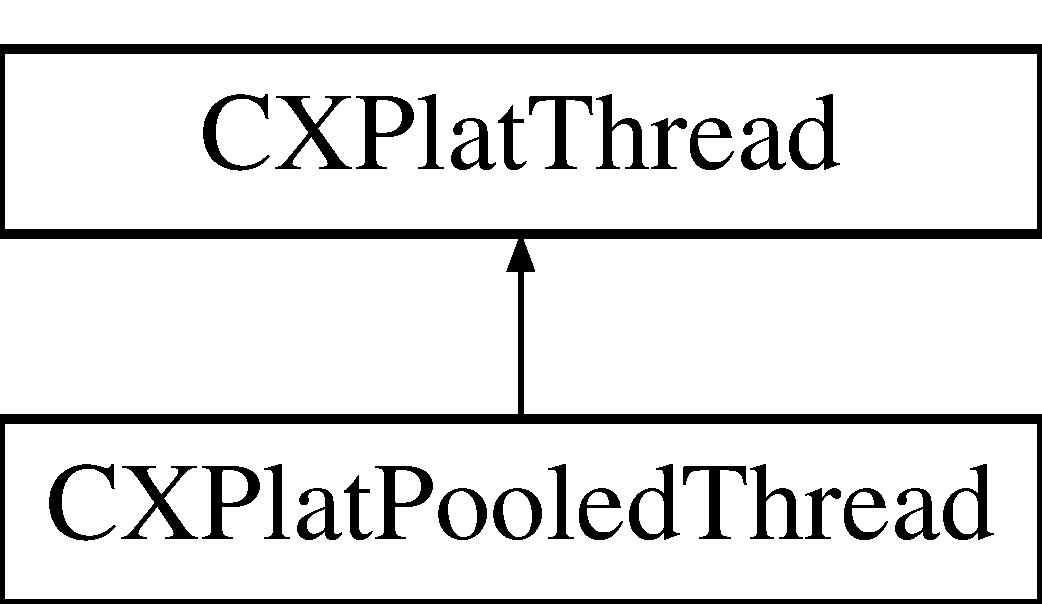
\includegraphics[height=2.000000cm]{class_c_x_plat_pooled_thread}
\end{center}
\end{figure}
\subsection*{\-Public \-Member \-Functions}
\begin{DoxyCompactItemize}
\item 
\hyperlink{class_c_x_plat_pooled_thread_ae83c999db18cc5efc0b1d7adfc3dc421}{\-C\-X\-Plat\-Pooled\-Thread} ()
\item 
virtual \hyperlink{class_c_x_plat_pooled_thread_ad5c141f6171340a1b5c3ea4c2b71dfde}{$\sim$\-C\-X\-Plat\-Pooled\-Thread} ()
\item 
virtual int \hyperlink{class_c_x_plat_pooled_thread_abe885544566fee0b5a07512c3202d120}{\-Start\-Working} ()
\item 
virtual \hyperlink{_cpclient_8h_a3be13892ae7076009afcf121347dd319}{\-B\-O\-O\-L} \hyperlink{class_c_x_plat_pooled_thread_a2024d59a6361c65af533f4b12501e6f3}{\-Is\-Thread\-Busy} ()
\begin{DoxyCompactList}\small\item\em \-Is thread in the user's code? \end{DoxyCompactList}\item 
\hyperlink{_cpclient_8h_a6464f7480a0fd0ee170cba12b2c0497f}{void} \hyperlink{class_c_x_plat_pooled_thread_a88375206dfba56aaef406774df8f23d1}{\-Set\-Completion\-Wait\-Time} (unsigned long l\-Wait\-Time)
\begin{DoxyCompactList}\small\item\em \-Set the max time we will wait for thread to finish work when we are ready to terminate it. \end{DoxyCompactList}\end{DoxyCompactItemize}
\subsection*{\-Protected \-Member \-Functions}
\begin{DoxyCompactItemize}
\item 
unsigned \hyperlink{class_c_x_plat_pooled_thread_a8b181531a0345e3e3b7381122766218f}{\-Worker\-Function} (\hyperlink{_cpclient_8h_a6464f7480a0fd0ee170cba12b2c0497f}{void} $\ast$p\-Param)
\item 
virtual unsigned \hyperlink{class_c_x_plat_pooled_thread_a398deb73c58c851f5f93a6b3d5ba5106}{\-Pooled\-Worker\-Function} ()=0
\end{DoxyCompactItemize}
\subsection*{\-Protected \-Attributes}
\begin{DoxyCompactItemize}
\item 
\hyperlink{class_c_x_plat_thread_pool}{\-C\-X\-Plat\-Thread\-Pool} $\ast$ \hyperlink{class_c_x_plat_pooled_thread_ad6ceff927d5ff0e06eec0d99aebb1b10}{p\-Pool\-Parent}
\item 
\hyperlink{class_c_x_plat_event}{\-C\-X\-Plat\-Event} \hyperlink{class_c_x_plat_pooled_thread_aa72050f5a65f4117e41aec984a976fac}{c\-Start\-Working}
\begin{DoxyCompactList}\small\item\em \-Pool that we belong to. \end{DoxyCompactList}\item 
\hyperlink{_cpclient_8h_a3be13892ae7076009afcf121347dd319}{\-B\-O\-O\-L} \hyperlink{class_c_x_plat_pooled_thread_ae9df7cdc87ca6ebf387fb4cf42836417}{b\-Thread\-Busy}
\begin{DoxyCompactList}\small\item\em \-When set, work starts. \end{DoxyCompactList}\item 
\hyperlink{_cpclient_8h_a3be13892ae7076009afcf121347dd319}{\-B\-O\-O\-L} \hyperlink{class_c_x_plat_pooled_thread_ab708ae971b8acdc4830987ea93ee4e52}{b\-Terminate\-Thread}
\item 
\hyperlink{_cpclient_8h_a3be13892ae7076009afcf121347dd319}{\-B\-O\-O\-L} \hyperlink{class_c_x_plat_pooled_thread_af269720f4a5cd4e294d9b5fa7aebd50a}{b\-Thread\-Allocated}
\item 
\hyperlink{_cpclient_8h_a6464f7480a0fd0ee170cba12b2c0497f}{void} $\ast$ \hyperlink{class_c_x_plat_pooled_thread_a76d10e5c387e927b7c3c553673e98a0c}{p\-Func\-Param}
\item 
unsigned long \hyperlink{class_c_x_plat_pooled_thread_a55185bc10d6367eaaf05fbd1e6ed3701}{l\-Wait\-For\-Completion}
\end{DoxyCompactItemize}
\subsection*{\-Friends}
\begin{DoxyCompactItemize}
\item 
class \hyperlink{class_c_x_plat_pooled_thread_ae6436844a6ddb7bc05268210cc9cdf3b}{\-C\-X\-Plat\-Thread\-Pool}
\begin{DoxyCompactList}\small\item\em \-So it can set the b\-Thread\-Allocated flag. \end{DoxyCompactList}\end{DoxyCompactItemize}


\subsection{\-Detailed \-Description}


\-Definition at line 55 of file \-C\-X\-Plat\-Pooled\-Thread.\-h.



\subsection{\-Constructor \& \-Destructor \-Documentation}
\hypertarget{class_c_x_plat_pooled_thread_ae83c999db18cc5efc0b1d7adfc3dc421}{\index{\-C\-X\-Plat\-Pooled\-Thread@{\-C\-X\-Plat\-Pooled\-Thread}!\-C\-X\-Plat\-Pooled\-Thread@{\-C\-X\-Plat\-Pooled\-Thread}}
\index{\-C\-X\-Plat\-Pooled\-Thread@{\-C\-X\-Plat\-Pooled\-Thread}!CXPlatPooledThread@{\-C\-X\-Plat\-Pooled\-Thread}}
\subsubsection[{\-C\-X\-Plat\-Pooled\-Thread}]{\setlength{\rightskip}{0pt plus 5cm}{\bf \-C\-X\-Plat\-Pooled\-Thread\-::\-C\-X\-Plat\-Pooled\-Thread} (
\begin{DoxyParamCaption}
{}
\end{DoxyParamCaption}
)}}\label{class_c_x_plat_pooled_thread_ae83c999db18cc5efc0b1d7adfc3dc421}


\-Definition at line 55 of file \-C\-X\-Plat\-Pooled\-Thread.\-cpp.

\hypertarget{class_c_x_plat_pooled_thread_ad5c141f6171340a1b5c3ea4c2b71dfde}{\index{\-C\-X\-Plat\-Pooled\-Thread@{\-C\-X\-Plat\-Pooled\-Thread}!$\sim$\-C\-X\-Plat\-Pooled\-Thread@{$\sim$\-C\-X\-Plat\-Pooled\-Thread}}
\index{$\sim$\-C\-X\-Plat\-Pooled\-Thread@{$\sim$\-C\-X\-Plat\-Pooled\-Thread}!CXPlatPooledThread@{\-C\-X\-Plat\-Pooled\-Thread}}
\subsubsection[{$\sim$\-C\-X\-Plat\-Pooled\-Thread}]{\setlength{\rightskip}{0pt plus 5cm}{\bf \-C\-X\-Plat\-Pooled\-Thread\-::$\sim$\-C\-X\-Plat\-Pooled\-Thread} (
\begin{DoxyParamCaption}
{}
\end{DoxyParamCaption}
)\hspace{0.3cm}{\ttfamily  \mbox{[}virtual\mbox{]}}}}\label{class_c_x_plat_pooled_thread_ad5c141f6171340a1b5c3ea4c2b71dfde}


\-Definition at line 62 of file \-C\-X\-Plat\-Pooled\-Thread.\-cpp.



\subsection{\-Member \-Function \-Documentation}
\hypertarget{class_c_x_plat_pooled_thread_a2024d59a6361c65af533f4b12501e6f3}{\index{\-C\-X\-Plat\-Pooled\-Thread@{\-C\-X\-Plat\-Pooled\-Thread}!\-Is\-Thread\-Busy@{\-Is\-Thread\-Busy}}
\index{\-Is\-Thread\-Busy@{\-Is\-Thread\-Busy}!CXPlatPooledThread@{\-C\-X\-Plat\-Pooled\-Thread}}
\subsubsection[{\-Is\-Thread\-Busy}]{\setlength{\rightskip}{0pt plus 5cm}{\bf \-B\-O\-O\-L} {\bf \-C\-X\-Plat\-Pooled\-Thread\-::\-Is\-Thread\-Busy} (
\begin{DoxyParamCaption}
{}
\end{DoxyParamCaption}
)\hspace{0.3cm}{\ttfamily  \mbox{[}virtual\mbox{]}}}}\label{class_c_x_plat_pooled_thread_a2024d59a6361c65af533f4b12501e6f3}


\-Is thread in the user's code? 



\-Definition at line 81 of file \-C\-X\-Plat\-Pooled\-Thread.\-cpp.

\hypertarget{class_c_x_plat_pooled_thread_a398deb73c58c851f5f93a6b3d5ba5106}{\index{\-C\-X\-Plat\-Pooled\-Thread@{\-C\-X\-Plat\-Pooled\-Thread}!\-Pooled\-Worker\-Function@{\-Pooled\-Worker\-Function}}
\index{\-Pooled\-Worker\-Function@{\-Pooled\-Worker\-Function}!CXPlatPooledThread@{\-C\-X\-Plat\-Pooled\-Thread}}
\subsubsection[{\-Pooled\-Worker\-Function}]{\setlength{\rightskip}{0pt plus 5cm}virtual unsigned {\bf \-C\-X\-Plat\-Pooled\-Thread\-::\-Pooled\-Worker\-Function} (
\begin{DoxyParamCaption}
{}
\end{DoxyParamCaption}
)\hspace{0.3cm}{\ttfamily  \mbox{[}protected, pure virtual\mbox{]}}}}\label{class_c_x_plat_pooled_thread_a398deb73c58c851f5f93a6b3d5ba5106}
\-This is what you should derive from to do your work. \-Note that once \-Pooled\-Worker\-Function returns, this thread is returned to the thread pool and you must request a new thread for any further work. \hypertarget{class_c_x_plat_pooled_thread_a88375206dfba56aaef406774df8f23d1}{\index{\-C\-X\-Plat\-Pooled\-Thread@{\-C\-X\-Plat\-Pooled\-Thread}!\-Set\-Completion\-Wait\-Time@{\-Set\-Completion\-Wait\-Time}}
\index{\-Set\-Completion\-Wait\-Time@{\-Set\-Completion\-Wait\-Time}!CXPlatPooledThread@{\-C\-X\-Plat\-Pooled\-Thread}}
\subsubsection[{\-Set\-Completion\-Wait\-Time}]{\setlength{\rightskip}{0pt plus 5cm}{\bf void} {\bf \-C\-X\-Plat\-Pooled\-Thread\-::\-Set\-Completion\-Wait\-Time} (
\begin{DoxyParamCaption}
\item[{unsigned long}]{l\-Wait\-Time}
\end{DoxyParamCaption}
)}}\label{class_c_x_plat_pooled_thread_a88375206dfba56aaef406774df8f23d1}


\-Set the max time we will wait for thread to finish work when we are ready to terminate it. 



\-Definition at line 117 of file \-C\-X\-Plat\-Pooled\-Thread.\-cpp.

\hypertarget{class_c_x_plat_pooled_thread_abe885544566fee0b5a07512c3202d120}{\index{\-C\-X\-Plat\-Pooled\-Thread@{\-C\-X\-Plat\-Pooled\-Thread}!\-Start\-Working@{\-Start\-Working}}
\index{\-Start\-Working@{\-Start\-Working}!CXPlatPooledThread@{\-C\-X\-Plat\-Pooled\-Thread}}
\subsubsection[{\-Start\-Working}]{\setlength{\rightskip}{0pt plus 5cm}int {\bf \-C\-X\-Plat\-Pooled\-Thread\-::\-Start\-Working} (
\begin{DoxyParamCaption}
{}
\end{DoxyParamCaption}
)\hspace{0.3cm}{\ttfamily  \mbox{[}virtual\mbox{]}}}}\label{class_c_x_plat_pooled_thread_abe885544566fee0b5a07512c3202d120}
\-Start doing the user's duty. \-N\-E\-V\-E\-R \-C\-A\-L\-L \-T\-H\-I\-S \-T\-W\-I\-C\-E! $\ast$$\ast$$\ast$$\ast$ \-After your \-Pooled\-Worker\-Function returns, this thread is added back to the thread pool! 

\-Definition at line 72 of file \-C\-X\-Plat\-Pooled\-Thread.\-cpp.

\hypertarget{class_c_x_plat_pooled_thread_a8b181531a0345e3e3b7381122766218f}{\index{\-C\-X\-Plat\-Pooled\-Thread@{\-C\-X\-Plat\-Pooled\-Thread}!\-Worker\-Function@{\-Worker\-Function}}
\index{\-Worker\-Function@{\-Worker\-Function}!CXPlatPooledThread@{\-C\-X\-Plat\-Pooled\-Thread}}
\subsubsection[{\-Worker\-Function}]{\setlength{\rightskip}{0pt plus 5cm}unsigned {\bf \-C\-X\-Plat\-Pooled\-Thread\-::\-Worker\-Function} (
\begin{DoxyParamCaption}
\item[{{\bf void} $\ast$}]{p\-Param}
\end{DoxyParamCaption}
)\hspace{0.3cm}{\ttfamily  \mbox{[}protected, virtual\mbox{]}}}}\label{class_c_x_plat_pooled_thread_a8b181531a0345e3e3b7381122766218f}
\-Implemented by this class. \-S\-H\-O\-U\-L\-D \-N\-O\-T \-B\-E \-D\-E\-R\-I\-V\-E\-D \-F\-R\-O\-M! \-Use \-Pooled\-Worker\-Function instead. 

\-Implements \hyperlink{class_c_x_plat_thread_af8a15900817f9673c6fd8e85cdedf27d}{\-C\-X\-Plat\-Thread}.



\-Definition at line 89 of file \-C\-X\-Plat\-Pooled\-Thread.\-cpp.



\subsection{\-Friends \-And \-Related \-Function \-Documentation}
\hypertarget{class_c_x_plat_pooled_thread_ae6436844a6ddb7bc05268210cc9cdf3b}{\index{\-C\-X\-Plat\-Pooled\-Thread@{\-C\-X\-Plat\-Pooled\-Thread}!\-C\-X\-Plat\-Thread\-Pool@{\-C\-X\-Plat\-Thread\-Pool}}
\index{\-C\-X\-Plat\-Thread\-Pool@{\-C\-X\-Plat\-Thread\-Pool}!CXPlatPooledThread@{\-C\-X\-Plat\-Pooled\-Thread}}
\subsubsection[{\-C\-X\-Plat\-Thread\-Pool}]{\setlength{\rightskip}{0pt plus 5cm}friend class {\bf \-C\-X\-Plat\-Thread\-Pool}\hspace{0.3cm}{\ttfamily  \mbox{[}friend\mbox{]}}}}\label{class_c_x_plat_pooled_thread_ae6436844a6ddb7bc05268210cc9cdf3b}


\-So it can set the b\-Thread\-Allocated flag. 



\-Definition at line 57 of file \-C\-X\-Plat\-Pooled\-Thread.\-h.



\subsection{\-Member \-Data \-Documentation}
\hypertarget{class_c_x_plat_pooled_thread_ab708ae971b8acdc4830987ea93ee4e52}{\index{\-C\-X\-Plat\-Pooled\-Thread@{\-C\-X\-Plat\-Pooled\-Thread}!b\-Terminate\-Thread@{b\-Terminate\-Thread}}
\index{b\-Terminate\-Thread@{b\-Terminate\-Thread}!CXPlatPooledThread@{\-C\-X\-Plat\-Pooled\-Thread}}
\subsubsection[{b\-Terminate\-Thread}]{\setlength{\rightskip}{0pt plus 5cm}{\bf \-B\-O\-O\-L} {\bf \-C\-X\-Plat\-Pooled\-Thread\-::b\-Terminate\-Thread}\hspace{0.3cm}{\ttfamily  \mbox{[}protected\mbox{]}}}}\label{class_c_x_plat_pooled_thread_ab708ae971b8acdc4830987ea93ee4e52}


\-Definition at line 85 of file \-C\-X\-Plat\-Pooled\-Thread.\-h.

\hypertarget{class_c_x_plat_pooled_thread_af269720f4a5cd4e294d9b5fa7aebd50a}{\index{\-C\-X\-Plat\-Pooled\-Thread@{\-C\-X\-Plat\-Pooled\-Thread}!b\-Thread\-Allocated@{b\-Thread\-Allocated}}
\index{b\-Thread\-Allocated@{b\-Thread\-Allocated}!CXPlatPooledThread@{\-C\-X\-Plat\-Pooled\-Thread}}
\subsubsection[{b\-Thread\-Allocated}]{\setlength{\rightskip}{0pt plus 5cm}{\bf \-B\-O\-O\-L} {\bf \-C\-X\-Plat\-Pooled\-Thread\-::b\-Thread\-Allocated}\hspace{0.3cm}{\ttfamily  \mbox{[}protected\mbox{]}}}}\label{class_c_x_plat_pooled_thread_af269720f4a5cd4e294d9b5fa7aebd50a}


\-Definition at line 86 of file \-C\-X\-Plat\-Pooled\-Thread.\-h.

\hypertarget{class_c_x_plat_pooled_thread_ae9df7cdc87ca6ebf387fb4cf42836417}{\index{\-C\-X\-Plat\-Pooled\-Thread@{\-C\-X\-Plat\-Pooled\-Thread}!b\-Thread\-Busy@{b\-Thread\-Busy}}
\index{b\-Thread\-Busy@{b\-Thread\-Busy}!CXPlatPooledThread@{\-C\-X\-Plat\-Pooled\-Thread}}
\subsubsection[{b\-Thread\-Busy}]{\setlength{\rightskip}{0pt plus 5cm}{\bf \-B\-O\-O\-L} {\bf \-C\-X\-Plat\-Pooled\-Thread\-::b\-Thread\-Busy}\hspace{0.3cm}{\ttfamily  \mbox{[}protected\mbox{]}}}}\label{class_c_x_plat_pooled_thread_ae9df7cdc87ca6ebf387fb4cf42836417}


\-When set, work starts. 



\-Definition at line 84 of file \-C\-X\-Plat\-Pooled\-Thread.\-h.

\hypertarget{class_c_x_plat_pooled_thread_aa72050f5a65f4117e41aec984a976fac}{\index{\-C\-X\-Plat\-Pooled\-Thread@{\-C\-X\-Plat\-Pooled\-Thread}!c\-Start\-Working@{c\-Start\-Working}}
\index{c\-Start\-Working@{c\-Start\-Working}!CXPlatPooledThread@{\-C\-X\-Plat\-Pooled\-Thread}}
\subsubsection[{c\-Start\-Working}]{\setlength{\rightskip}{0pt plus 5cm}{\bf \-C\-X\-Plat\-Event} {\bf \-C\-X\-Plat\-Pooled\-Thread\-::c\-Start\-Working}\hspace{0.3cm}{\ttfamily  \mbox{[}protected\mbox{]}}}}\label{class_c_x_plat_pooled_thread_aa72050f5a65f4117e41aec984a976fac}


\-Pool that we belong to. 



\-Definition at line 83 of file \-C\-X\-Plat\-Pooled\-Thread.\-h.

\hypertarget{class_c_x_plat_pooled_thread_a55185bc10d6367eaaf05fbd1e6ed3701}{\index{\-C\-X\-Plat\-Pooled\-Thread@{\-C\-X\-Plat\-Pooled\-Thread}!l\-Wait\-For\-Completion@{l\-Wait\-For\-Completion}}
\index{l\-Wait\-For\-Completion@{l\-Wait\-For\-Completion}!CXPlatPooledThread@{\-C\-X\-Plat\-Pooled\-Thread}}
\subsubsection[{l\-Wait\-For\-Completion}]{\setlength{\rightskip}{0pt plus 5cm}unsigned long {\bf \-C\-X\-Plat\-Pooled\-Thread\-::l\-Wait\-For\-Completion}\hspace{0.3cm}{\ttfamily  \mbox{[}protected\mbox{]}}}}\label{class_c_x_plat_pooled_thread_a55185bc10d6367eaaf05fbd1e6ed3701}


\-Definition at line 88 of file \-C\-X\-Plat\-Pooled\-Thread.\-h.

\hypertarget{class_c_x_plat_pooled_thread_a76d10e5c387e927b7c3c553673e98a0c}{\index{\-C\-X\-Plat\-Pooled\-Thread@{\-C\-X\-Plat\-Pooled\-Thread}!p\-Func\-Param@{p\-Func\-Param}}
\index{p\-Func\-Param@{p\-Func\-Param}!CXPlatPooledThread@{\-C\-X\-Plat\-Pooled\-Thread}}
\subsubsection[{p\-Func\-Param}]{\setlength{\rightskip}{0pt plus 5cm}{\bf void}$\ast$ {\bf \-C\-X\-Plat\-Pooled\-Thread\-::p\-Func\-Param}\hspace{0.3cm}{\ttfamily  \mbox{[}protected\mbox{]}}}}\label{class_c_x_plat_pooled_thread_a76d10e5c387e927b7c3c553673e98a0c}


\-Definition at line 87 of file \-C\-X\-Plat\-Pooled\-Thread.\-h.

\hypertarget{class_c_x_plat_pooled_thread_ad6ceff927d5ff0e06eec0d99aebb1b10}{\index{\-C\-X\-Plat\-Pooled\-Thread@{\-C\-X\-Plat\-Pooled\-Thread}!p\-Pool\-Parent@{p\-Pool\-Parent}}
\index{p\-Pool\-Parent@{p\-Pool\-Parent}!CXPlatPooledThread@{\-C\-X\-Plat\-Pooled\-Thread}}
\subsubsection[{p\-Pool\-Parent}]{\setlength{\rightskip}{0pt plus 5cm}{\bf \-C\-X\-Plat\-Thread\-Pool}$\ast$ {\bf \-C\-X\-Plat\-Pooled\-Thread\-::p\-Pool\-Parent}\hspace{0.3cm}{\ttfamily  \mbox{[}protected\mbox{]}}}}\label{class_c_x_plat_pooled_thread_ad6ceff927d5ff0e06eec0d99aebb1b10}


\-Definition at line 82 of file \-C\-X\-Plat\-Pooled\-Thread.\-h.



\-The documentation for this class was generated from the following files\-:\begin{DoxyCompactItemize}
\item 
common/\hyperlink{_c_x_plat_pooled_thread_8h}{\-C\-X\-Plat\-Pooled\-Thread.\-h}\item 
common/\hyperlink{_c_x_plat_pooled_thread_8cpp}{\-C\-X\-Plat\-Pooled\-Thread.\-cpp}\end{DoxyCompactItemize}

\hypertarget{class_c_x_plat_process}{\section{\-C\-X\-Plat\-Process \-Class \-Reference}
\label{class_c_x_plat_process}\index{\-C\-X\-Plat\-Process@{\-C\-X\-Plat\-Process}}
}


\-\_\-\-M\-S\-C\-\_\-\-V\-E\-R $>$ 1000  




{\ttfamily \#include $<$\-C\-X\-Plat\-Process.\-h$>$}

\subsection*{\-Public \-Member \-Functions}
\begin{DoxyCompactItemize}
\item 
\hyperlink{class_c_x_plat_process_ad31bcf12947c3e94d3d08e3e04b5f009}{\-C\-X\-Plat\-Process} ()
\item 
\hyperlink{class_c_x_plat_process_adbba672243c0f6031ad3acc6a0742725}{\-C\-X\-Plat\-Process} (char $\ast$sz\-Process, \hyperlink{_cpclient_8h_a3be13892ae7076009afcf121347dd319}{\-B\-O\-O\-L} b\-Hide=\hyperlink{_x_plat_8h_aa8cecfc5c5c054d2875c03e77b7be15d}{\-T\-R\-U\-E}, \hyperlink{_cpclient_8h_a3be13892ae7076009afcf121347dd319}{\-B\-O\-O\-L} b\-Wait=\hyperlink{_x_plat_8h_aa93f0eb578d23995850d61f7d61c55c1}{\-F\-A\-L\-S\-E}, \hyperlink{_cpclient_8h_a3be13892ae7076009afcf121347dd319}{\-B\-O\-O\-L} b\-Inherit\-Handles=\hyperlink{_x_plat_8h_aa8cecfc5c5c054d2875c03e77b7be15d}{\-T\-R\-U\-E})
\item 
virtual \hyperlink{class_c_x_plat_process_a2d556f26349a1c42d2a851ba15985a8c}{$\sim$\-C\-X\-Plat\-Process} ()
\item 
int \hyperlink{class_c_x_plat_process_aadd87f5c163cbbdceb47607e7e72b462}{\-Launch} (char $\ast$sz\-Process, \hyperlink{_cpclient_8h_a3be13892ae7076009afcf121347dd319}{\-B\-O\-O\-L} b\-Hide=\hyperlink{_x_plat_8h_aa8cecfc5c5c054d2875c03e77b7be15d}{\-T\-R\-U\-E}, \hyperlink{_cpclient_8h_a3be13892ae7076009afcf121347dd319}{\-B\-O\-O\-L} b\-Wait=\hyperlink{_x_plat_8h_aa93f0eb578d23995850d61f7d61c55c1}{\-F\-A\-L\-S\-E}, \hyperlink{_cpclient_8h_a3be13892ae7076009afcf121347dd319}{\-B\-O\-O\-L} b\-Inherit\-Handles=\hyperlink{_x_plat_8h_aa8cecfc5c5c054d2875c03e77b7be15d}{\-T\-R\-U\-E})
\begin{DoxyCompactList}\small\item\em \-Launch and return process \-I\-D (\-N\-T) \end{DoxyCompactList}\item 
\hyperlink{_x_plat_8h_af3c5c1485bb09f4be888d78cdaf93e00}{\-X\-P\-L\-A\-T\-\_\-\-H\-A\-N\-D\-L\-E} \hyperlink{class_c_x_plat_process_a498f7e51e46120ab44bce6951e5cccb3}{\-Get\-Process\-Handle} ()
\end{DoxyCompactItemize}
\subsection*{\-Protected \-Member \-Functions}
\begin{DoxyCompactItemize}
\item 
int \hyperlink{class_c_x_plat_process_a67688c196fa45a83e4f73817ab42da78}{\-Launch\-Hidden\-Process} (char $\ast$sz\-Process, \hyperlink{_cpclient_8h_a3be13892ae7076009afcf121347dd319}{\-B\-O\-O\-L} b\-Hide=\hyperlink{_x_plat_8h_aa8cecfc5c5c054d2875c03e77b7be15d}{\-T\-R\-U\-E}, \hyperlink{_cpclient_8h_a3be13892ae7076009afcf121347dd319}{\-B\-O\-O\-L} b\-Wait=\hyperlink{_x_plat_8h_aa93f0eb578d23995850d61f7d61c55c1}{\-F\-A\-L\-S\-E}, \hyperlink{_cpclient_8h_a3be13892ae7076009afcf121347dd319}{\-B\-O\-O\-L} b\-Inherit\-Handles=\hyperlink{_x_plat_8h_aa8cecfc5c5c054d2875c03e77b7be15d}{\-T\-R\-U\-E})
\begin{DoxyCompactList}\small\item\em \-Launch a process hidden (this is mostly for \-Windows) \end{DoxyCompactList}\end{DoxyCompactItemize}
\subsection*{\-Protected \-Attributes}
\begin{DoxyCompactItemize}
\item 
\hyperlink{_x_plat_8h_af3c5c1485bb09f4be888d78cdaf93e00}{\-X\-P\-L\-A\-T\-\_\-\-H\-A\-N\-D\-L\-E} \hyperlink{class_c_x_plat_process_a88a0f67e49bac8b19cdc651eb25072e6}{h\-Process}
\end{DoxyCompactItemize}


\subsection{\-Detailed \-Description}
\-\_\-\-M\-S\-C\-\_\-\-V\-E\-R $>$ 1000 

\-Launch a separate process \-Class to launch a process 

\-Definition at line 31 of file \-C\-X\-Plat\-Process.\-h.



\subsection{\-Constructor \& \-Destructor \-Documentation}
\hypertarget{class_c_x_plat_process_ad31bcf12947c3e94d3d08e3e04b5f009}{\index{\-C\-X\-Plat\-Process@{\-C\-X\-Plat\-Process}!\-C\-X\-Plat\-Process@{\-C\-X\-Plat\-Process}}
\index{\-C\-X\-Plat\-Process@{\-C\-X\-Plat\-Process}!CXPlatProcess@{\-C\-X\-Plat\-Process}}
\subsubsection[{\-C\-X\-Plat\-Process}]{\setlength{\rightskip}{0pt plus 5cm}{\bf \-C\-X\-Plat\-Process\-::\-C\-X\-Plat\-Process} (
\begin{DoxyParamCaption}
{}
\end{DoxyParamCaption}
)}}\label{class_c_x_plat_process_ad31bcf12947c3e94d3d08e3e04b5f009}


\-Definition at line 29 of file \-C\-X\-Plat\-Process.\-cpp.

\hypertarget{class_c_x_plat_process_adbba672243c0f6031ad3acc6a0742725}{\index{\-C\-X\-Plat\-Process@{\-C\-X\-Plat\-Process}!\-C\-X\-Plat\-Process@{\-C\-X\-Plat\-Process}}
\index{\-C\-X\-Plat\-Process@{\-C\-X\-Plat\-Process}!CXPlatProcess@{\-C\-X\-Plat\-Process}}
\subsubsection[{\-C\-X\-Plat\-Process}]{\setlength{\rightskip}{0pt plus 5cm}{\bf \-C\-X\-Plat\-Process\-::\-C\-X\-Plat\-Process} (
\begin{DoxyParamCaption}
\item[{char $\ast$}]{sz\-Process, }
\item[{{\bf \-B\-O\-O\-L}}]{b\-Hide = {\ttfamily {\bf \-T\-R\-U\-E}}, }
\item[{{\bf \-B\-O\-O\-L}}]{b\-Wait = {\ttfamily {\bf \-F\-A\-L\-S\-E}}, }
\item[{{\bf \-B\-O\-O\-L}}]{b\-Inherit\-Handles = {\ttfamily {\bf \-T\-R\-U\-E}}}
\end{DoxyParamCaption}
)}}\label{class_c_x_plat_process_adbba672243c0f6031ad3acc6a0742725}


\-Definition at line 34 of file \-C\-X\-Plat\-Process.\-cpp.

\hypertarget{class_c_x_plat_process_a2d556f26349a1c42d2a851ba15985a8c}{\index{\-C\-X\-Plat\-Process@{\-C\-X\-Plat\-Process}!$\sim$\-C\-X\-Plat\-Process@{$\sim$\-C\-X\-Plat\-Process}}
\index{$\sim$\-C\-X\-Plat\-Process@{$\sim$\-C\-X\-Plat\-Process}!CXPlatProcess@{\-C\-X\-Plat\-Process}}
\subsubsection[{$\sim$\-C\-X\-Plat\-Process}]{\setlength{\rightskip}{0pt plus 5cm}{\bf \-C\-X\-Plat\-Process\-::$\sim$\-C\-X\-Plat\-Process} (
\begin{DoxyParamCaption}
{}
\end{DoxyParamCaption}
)\hspace{0.3cm}{\ttfamily  \mbox{[}virtual\mbox{]}}}}\label{class_c_x_plat_process_a2d556f26349a1c42d2a851ba15985a8c}


\-Definition at line 41 of file \-C\-X\-Plat\-Process.\-cpp.



\subsection{\-Member \-Function \-Documentation}
\hypertarget{class_c_x_plat_process_a498f7e51e46120ab44bce6951e5cccb3}{\index{\-C\-X\-Plat\-Process@{\-C\-X\-Plat\-Process}!\-Get\-Process\-Handle@{\-Get\-Process\-Handle}}
\index{\-Get\-Process\-Handle@{\-Get\-Process\-Handle}!CXPlatProcess@{\-C\-X\-Plat\-Process}}
\subsubsection[{\-Get\-Process\-Handle}]{\setlength{\rightskip}{0pt plus 5cm}{\bf \-X\-P\-L\-A\-T\-\_\-\-H\-A\-N\-D\-L\-E} {\bf \-C\-X\-Plat\-Process\-::\-Get\-Process\-Handle} (
\begin{DoxyParamCaption}
\item[{{\bf void}}]{}
\end{DoxyParamCaption}
)}}\label{class_c_x_plat_process_a498f7e51e46120ab44bce6951e5cccb3}


\-Definition at line 50 of file \-C\-X\-Plat\-Process.\-cpp.

\hypertarget{class_c_x_plat_process_aadd87f5c163cbbdceb47607e7e72b462}{\index{\-C\-X\-Plat\-Process@{\-C\-X\-Plat\-Process}!\-Launch@{\-Launch}}
\index{\-Launch@{\-Launch}!CXPlatProcess@{\-C\-X\-Plat\-Process}}
\subsubsection[{\-Launch}]{\setlength{\rightskip}{0pt plus 5cm}int {\bf \-C\-X\-Plat\-Process\-::\-Launch} (
\begin{DoxyParamCaption}
\item[{char $\ast$}]{sz\-Process, }
\item[{{\bf \-B\-O\-O\-L}}]{b\-Hide = {\ttfamily {\bf \-T\-R\-U\-E}}, }
\item[{{\bf \-B\-O\-O\-L}}]{b\-Wait = {\ttfamily {\bf \-F\-A\-L\-S\-E}}, }
\item[{{\bf \-B\-O\-O\-L}}]{b\-Inherit\-Handles = {\ttfamily {\bf \-T\-R\-U\-E}}}
\end{DoxyParamCaption}
)}}\label{class_c_x_plat_process_aadd87f5c163cbbdceb47607e7e72b462}


\-Launch and return process \-I\-D (\-N\-T) 



\-Definition at line 45 of file \-C\-X\-Plat\-Process.\-cpp.

\hypertarget{class_c_x_plat_process_a67688c196fa45a83e4f73817ab42da78}{\index{\-C\-X\-Plat\-Process@{\-C\-X\-Plat\-Process}!\-Launch\-Hidden\-Process@{\-Launch\-Hidden\-Process}}
\index{\-Launch\-Hidden\-Process@{\-Launch\-Hidden\-Process}!CXPlatProcess@{\-C\-X\-Plat\-Process}}
\subsubsection[{\-Launch\-Hidden\-Process}]{\setlength{\rightskip}{0pt plus 5cm}int {\bf \-C\-X\-Plat\-Process\-::\-Launch\-Hidden\-Process} (
\begin{DoxyParamCaption}
\item[{char $\ast$}]{sz\-Process, }
\item[{{\bf \-B\-O\-O\-L}}]{b\-Hide = {\ttfamily {\bf \-T\-R\-U\-E}}, }
\item[{{\bf \-B\-O\-O\-L}}]{b\-Wait = {\ttfamily {\bf \-F\-A\-L\-S\-E}}, }
\item[{{\bf \-B\-O\-O\-L}}]{b\-Inherit\-Handles = {\ttfamily {\bf \-T\-R\-U\-E}}}
\end{DoxyParamCaption}
)\hspace{0.3cm}{\ttfamily  \mbox{[}protected\mbox{]}}}}\label{class_c_x_plat_process_a67688c196fa45a83e4f73817ab42da78}


\-Launch a process hidden (this is mostly for \-Windows) 



\-Definition at line 56 of file \-C\-X\-Plat\-Process.\-cpp.



\subsection{\-Member \-Data \-Documentation}
\hypertarget{class_c_x_plat_process_a88a0f67e49bac8b19cdc651eb25072e6}{\index{\-C\-X\-Plat\-Process@{\-C\-X\-Plat\-Process}!h\-Process@{h\-Process}}
\index{h\-Process@{h\-Process}!CXPlatProcess@{\-C\-X\-Plat\-Process}}
\subsubsection[{h\-Process}]{\setlength{\rightskip}{0pt plus 5cm}{\bf \-X\-P\-L\-A\-T\-\_\-\-H\-A\-N\-D\-L\-E} {\bf \-C\-X\-Plat\-Process\-::h\-Process}\hspace{0.3cm}{\ttfamily  \mbox{[}protected\mbox{]}}}}\label{class_c_x_plat_process_a88a0f67e49bac8b19cdc651eb25072e6}


\-Definition at line 48 of file \-C\-X\-Plat\-Process.\-h.



\-The documentation for this class was generated from the following files\-:\begin{DoxyCompactItemize}
\item 
common/\hyperlink{_c_x_plat_process_8h}{\-C\-X\-Plat\-Process.\-h}\item 
common/\hyperlink{_c_x_plat_process_8cpp}{\-C\-X\-Plat\-Process.\-cpp}\end{DoxyCompactItemize}

\hypertarget{class_c_x_plat_thread}{\section{\-C\-X\-Plat\-Thread \-Class \-Reference}
\label{class_c_x_plat_thread}\index{\-C\-X\-Plat\-Thread@{\-C\-X\-Plat\-Thread}}
}


\hyperlink{_c_x_plat_thread_8h}{\-C\-X\-Plat\-Thread.\-h}\-: interface for the \hyperlink{class_c_x_plat_thread}{\-C\-X\-Plat\-Thread} class.  




{\ttfamily \#include $<$\-C\-X\-Plat\-Thread.\-h$>$}

\-Inheritance diagram for \-C\-X\-Plat\-Thread\-:\begin{figure}[H]
\begin{center}
\leavevmode
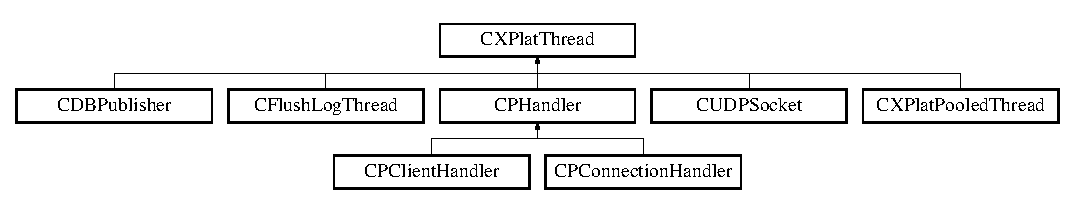
\includegraphics[height=2.301370cm]{class_c_x_plat_thread}
\end{center}
\end{figure}
\subsection*{\-Public \-Types}
\begin{DoxyCompactItemize}
\item 
enum \hyperlink{class_c_x_plat_thread_a15b8bc4370560890e1a1ae0dce671c01}{\-T\-H\-R\-E\-A\-D\-\_\-\-S\-T\-A\-T\-U\-S} \{ \*
\hyperlink{class_c_x_plat_thread_a15b8bc4370560890e1a1ae0dce671c01ad690f503ed52e84a4f3f6fa6e7e45b8b}{\-T\-H\-R\-E\-A\-D\-\_\-\-S\-U\-C\-C\-E\-S\-S} =  0, 
\hyperlink{class_c_x_plat_thread_a15b8bc4370560890e1a1ae0dce671c01a85f85b8c4e331da05995a226a512150b}{\-N\-O\-T\-\_\-\-S\-T\-A\-R\-T\-E\-D} =  1, 
\hyperlink{class_c_x_plat_thread_a15b8bc4370560890e1a1ae0dce671c01ad7fcefbaab4a06bc3814466a1faf7987}{\-S\-U\-S\-P\-E\-N\-D\-E\-D} =  2, 
\hyperlink{class_c_x_plat_thread_a15b8bc4370560890e1a1ae0dce671c01a2cb33518684a999f5dc00146f87b2682}{\-R\-E\-S\-U\-M\-E\-D} =  3, 
\*
\hyperlink{class_c_x_plat_thread_a15b8bc4370560890e1a1ae0dce671c01ae23d2a18cc876c05165d4848b163fa99}{\-R\-U\-N\-N\-I\-N\-G} =  4, 
\hyperlink{class_c_x_plat_thread_a15b8bc4370560890e1a1ae0dce671c01aaf29b416710281928ad716461bb322da}{\-C\-A\-N\-T\-\_\-\-S\-T\-A\-R\-T} =  5, 
\hyperlink{class_c_x_plat_thread_a15b8bc4370560890e1a1ae0dce671c01ae0213d5c510838b55938a9ed76217b36}{\-A\-L\-R\-E\-A\-D\-Y\-\_\-\-S\-U\-S\-P\-E\-N\-D\-E\-D} =  6, 
\hyperlink{class_c_x_plat_thread_a15b8bc4370560890e1a1ae0dce671c01ac3cf31918d7ef196c6f0eca2bc3d6555}{\-T\-H\-R\-E\-A\-D\-\_\-\-T\-E\-R\-M\-I\-N\-A\-T\-E\-D} =  7, 
\*
\hyperlink{class_c_x_plat_thread_a15b8bc4370560890e1a1ae0dce671c01a851b62a0b0daf4518f0e1341c7002049}{\-N\-O\-T\-\_\-\-S\-U\-P\-P\-O\-R\-T\-E\-D\-\_\-\-O\-N\-\_\-\-P\-L\-A\-T\-F\-O\-R\-M} =  8, 
\hyperlink{class_c_x_plat_thread_a15b8bc4370560890e1a1ae0dce671c01a49d7b2b48d143f09ac78515689fb9d94}{\-I\-N\-V\-A\-L\-I\-D\-\_\-\-R\-E\-Q\-U\-E\-S\-T} =  9, 
\hyperlink{class_c_x_plat_thread_a15b8bc4370560890e1a1ae0dce671c01af58795605d44445786b30d841a9998e8}{\-A\-L\-R\-E\-A\-D\-Y\-\_\-\-R\-U\-N\-N\-I\-N\-G} =  10
 \}
\begin{DoxyCompactList}\small\item\em \-Current status of threads. \end{DoxyCompactList}\end{DoxyCompactItemize}
\subsection*{\-Public \-Member \-Functions}
\begin{DoxyCompactItemize}
\item 
\hyperlink{class_c_x_plat_thread_a1eb15fa5d9fd621822bce0ef40cc25ed}{\-C\-X\-Plat\-Thread} ()
\item 
virtual \hyperlink{class_c_x_plat_thread_a3ce5dcd1f7b89fe1aff7650914d8e2c9}{$\sim$\-C\-X\-Plat\-Thread} ()
\item 
virtual \hyperlink{class_c_x_plat_thread_a15b8bc4370560890e1a1ae0dce671c01}{\-T\-H\-R\-E\-A\-D\-\_\-\-S\-T\-A\-T\-U\-S} \hyperlink{class_c_x_plat_thread_a9ebb03bd1483413fbcbdb6510a67167f}{\-Start\-Thread} (\hyperlink{_cpclient_8h_a6464f7480a0fd0ee170cba12b2c0497f}{void} $\ast$p\-Param=\-N\-U\-L\-L, \hyperlink{_cpclient_8h_a3be13892ae7076009afcf121347dd319}{\-B\-O\-O\-L} b\-Start\-Suspended=\hyperlink{_x_plat_8h_aa93f0eb578d23995850d61f7d61c55c1}{\-F\-A\-L\-S\-E})
\item 
virtual \hyperlink{class_c_x_plat_thread_a15b8bc4370560890e1a1ae0dce671c01}{\-T\-H\-R\-E\-A\-D\-\_\-\-S\-T\-A\-T\-U\-S} \hyperlink{class_c_x_plat_thread_a1f6aeadb170ca467a5a07cde7104e362}{\-Suspend\-Thread} ()
\begin{DoxyCompactList}\small\item\em \-Suspend thread. \end{DoxyCompactList}\item 
virtual \hyperlink{class_c_x_plat_thread_a15b8bc4370560890e1a1ae0dce671c01}{\-T\-H\-R\-E\-A\-D\-\_\-\-S\-T\-A\-T\-U\-S} \hyperlink{class_c_x_plat_thread_ab8332931990edf82093e5905d4fd2c36}{\-Resume\-Thread} ()
\begin{DoxyCompactList}\small\item\em \-Resume thread. \end{DoxyCompactList}\item 
virtual \hyperlink{_x_plat_8h_af3c5c1485bb09f4be888d78cdaf93e00}{\-X\-P\-L\-A\-T\-\_\-\-H\-A\-N\-D\-L\-E} \hyperlink{class_c_x_plat_thread_a18d5ad4291e0adb5c54694043aebd4f2}{\-Get\-Thread\-Handle} ()
\begin{DoxyCompactList}\small\item\em \-Return the thread handle. \end{DoxyCompactList}\item 
virtual \hyperlink{class_c_x_plat_thread_a15b8bc4370560890e1a1ae0dce671c01}{\-T\-H\-R\-E\-A\-D\-\_\-\-S\-T\-A\-T\-U\-S} \hyperlink{class_c_x_plat_thread_a5f60c36cb20e3b5d85d8ef506d9d8bf1}{\-Get\-Thread\-Status} ()
\begin{DoxyCompactList}\small\item\em \-Check to see if thread is active. \end{DoxyCompactList}\item 
virtual \hyperlink{_x_plat_8h_aa39b39d94407451a6ec0226479db68cf}{\-D\-W\-O\-R\-D} \hyperlink{class_c_x_plat_thread_ab68b6494893d24b365e317bff78b3a9e}{\-Wait\-For\-Thread\-Completion} (\hyperlink{_x_plat_8h_aa39b39d94407451a6ec0226479db68cf}{\-D\-W\-O\-R\-D} dw\-Timeout=\hyperlink{_x_plat_8h_aa84a29002ab81c719c0d07bb446296e0}{\-I\-N\-F\-I\-N\-I\-T\-E})
\begin{DoxyCompactList}\small\item\em \-Wait for a thread to termintate. \end{DoxyCompactList}\item 
virtual int \hyperlink{class_c_x_plat_thread_a1ed5f6517c305e9cfa981a60a0d191e7}{\-Get\-Thread\-Type} ()
\begin{DoxyCompactList}\small\item\em \-Return a user defined thread type \-I\-D. \end{DoxyCompactList}\item 
virtual int \hyperlink{class_c_x_plat_thread_ae85703ff3ca0b8516f1a0e75bd937667}{\-Detach\-Thread} ()
\begin{DoxyCompactList}\small\item\em \-You must either detach the thread or join it for proper cleanup. \end{DoxyCompactList}\end{DoxyCompactItemize}
\subsection*{\-Static \-Public \-Member \-Functions}
\begin{DoxyCompactItemize}
\item 
static \hyperlink{_cpclient_8h_a3be13892ae7076009afcf121347dd319}{\-B\-O\-O\-L} \hyperlink{class_c_x_plat_thread_aeb38ce2a0b264d0da5c3c5d26460f851}{\-Is\-Thread\-Active} (\hyperlink{_x_plat_8h_af3c5c1485bb09f4be888d78cdaf93e00}{\-X\-P\-L\-A\-T\-\_\-\-H\-A\-N\-D\-L\-E} h\-Thread)
\begin{DoxyCompactList}\small\item\em \-Check to see if a thread is active. \end{DoxyCompactList}\end{DoxyCompactItemize}
\subsection*{\-Protected \-Member \-Functions}
\begin{DoxyCompactItemize}
\item 
virtual unsigned \hyperlink{class_c_x_plat_thread_af8a15900817f9673c6fd8e85cdedf27d}{\-Worker\-Function} (\hyperlink{_cpclient_8h_a6464f7480a0fd0ee170cba12b2c0497f}{void} $\ast$p\-Param)=0
\begin{DoxyCompactList}\small\item\em \-Called by \hyperlink{class_c_x_plat_thread}{\-C\-X\-Plat\-Thread} to start work in object context. \end{DoxyCompactList}\item 
\hyperlink{_cpclient_8h_a6464f7480a0fd0ee170cba12b2c0497f}{void} \hyperlink{class_c_x_plat_thread_aa7337490cd6399730aaeee9497835455}{\-Close\-Thread\-Handle} ()
\begin{DoxyCompactList}\small\item\em \-Close handle. \end{DoxyCompactList}\end{DoxyCompactItemize}
\subsection*{\-Protected \-Attributes}
\begin{DoxyCompactItemize}
\item 
\hyperlink{_cpclient_8h_a3be13892ae7076009afcf121347dd319}{\-B\-O\-O\-L} \hyperlink{class_c_x_plat_thread_a91939e9102e3d7a3be728e861e2e4344}{b\-Suspended}
\item 
\hyperlink{_x_plat_8h_af3c5c1485bb09f4be888d78cdaf93e00}{\-X\-P\-L\-A\-T\-\_\-\-H\-A\-N\-D\-L\-E} \hyperlink{class_c_x_plat_thread_af20b7c1d6babaa0ecb429d3e6d846cc4}{h\-Thread\-Handle}
\item 
\hyperlink{_cpclient_8h_a6464f7480a0fd0ee170cba12b2c0497f}{void} $\ast$ \hyperlink{class_c_x_plat_thread_a836a233113a162ba4628478b1e230dcf}{p\-User\-Parm}
\item 
\hyperlink{_cpclient_8h_a3be13892ae7076009afcf121347dd319}{\-B\-O\-O\-L} \hyperlink{class_c_x_plat_thread_aebdedede286d9cf03841c44615478e4a}{b\-Detached}
\item 
\hyperlink{_cpclient_8h_a3be13892ae7076009afcf121347dd319}{\-B\-O\-O\-L} \hyperlink{class_c_x_plat_thread_a15720f77b93771acd0d2b59f042eb8d6}{b\-Joined}
\end{DoxyCompactItemize}


\subsection{\-Detailed \-Description}
\hyperlink{_c_x_plat_thread_8h}{\-C\-X\-Plat\-Thread.\-h}\-: interface for the \hyperlink{class_c_x_plat_thread}{\-C\-X\-Plat\-Thread} class. 

\-Created\-: \-Richard \-A. \-Bross \-N\-O\-T\-E\-S\-: \-On \-Unix platforms, every thread must be either detached or \-Wait\-For\-Thread\-Completion(\-I\-N\-F\-I\-N\-I\-T\-E) must be called for proper cleanup. \-If \-Wait\-For\-Thread\-Completion is called with any timeout other than \-I\-N\-F\-I\-N\-I\-T\-E, and it times out, you must then call either \-Detach\-Thread or \-Wait\-For\-Thread\-Completion(\-I\-N\-F\-I\-N\-I\-T\-E) if you wish to ensure proper cleanup prior to detruction of the object..

\-However, if neither has been called, and the object is deleted the destructor will automatically call \-Wait\-For\-Thread\-Completion(\-I\-N\-F\-I\-N\-I\-T\-E). \-\_\-\-M\-S\-C\-\_\-\-V\-E\-R $>$= 1000 

\-Definition at line 43 of file \-C\-X\-Plat\-Thread.\-h.



\subsection{\-Member \-Enumeration \-Documentation}
\hypertarget{class_c_x_plat_thread_a15b8bc4370560890e1a1ae0dce671c01}{\index{\-C\-X\-Plat\-Thread@{\-C\-X\-Plat\-Thread}!\-T\-H\-R\-E\-A\-D\-\_\-\-S\-T\-A\-T\-U\-S@{\-T\-H\-R\-E\-A\-D\-\_\-\-S\-T\-A\-T\-U\-S}}
\index{\-T\-H\-R\-E\-A\-D\-\_\-\-S\-T\-A\-T\-U\-S@{\-T\-H\-R\-E\-A\-D\-\_\-\-S\-T\-A\-T\-U\-S}!CXPlatThread@{\-C\-X\-Plat\-Thread}}
\subsubsection[{\-T\-H\-R\-E\-A\-D\-\_\-\-S\-T\-A\-T\-U\-S}]{\setlength{\rightskip}{0pt plus 5cm}enum {\bf \-C\-X\-Plat\-Thread\-::\-T\-H\-R\-E\-A\-D\-\_\-\-S\-T\-A\-T\-U\-S}}}\label{class_c_x_plat_thread_a15b8bc4370560890e1a1ae0dce671c01}


\-Current status of threads. 

\begin{Desc}
\item[\-Enumerator\-: ]\par
\begin{description}
\index{\-T\-H\-R\-E\-A\-D\-\_\-\-S\-U\-C\-C\-E\-S\-S@{\-T\-H\-R\-E\-A\-D\-\_\-\-S\-U\-C\-C\-E\-S\-S}!\-C\-X\-Plat\-Thread@{\-C\-X\-Plat\-Thread}}\index{\-C\-X\-Plat\-Thread@{\-C\-X\-Plat\-Thread}!\-T\-H\-R\-E\-A\-D\-\_\-\-S\-U\-C\-C\-E\-S\-S@{\-T\-H\-R\-E\-A\-D\-\_\-\-S\-U\-C\-C\-E\-S\-S}}\item[{\em 
\hypertarget{class_c_x_plat_thread_a15b8bc4370560890e1a1ae0dce671c01ad690f503ed52e84a4f3f6fa6e7e45b8b}{\-T\-H\-R\-E\-A\-D\-\_\-\-S\-U\-C\-C\-E\-S\-S}\label{class_c_x_plat_thread_a15b8bc4370560890e1a1ae0dce671c01ad690f503ed52e84a4f3f6fa6e7e45b8b}
}]\index{\-N\-O\-T\-\_\-\-S\-T\-A\-R\-T\-E\-D@{\-N\-O\-T\-\_\-\-S\-T\-A\-R\-T\-E\-D}!\-C\-X\-Plat\-Thread@{\-C\-X\-Plat\-Thread}}\index{\-C\-X\-Plat\-Thread@{\-C\-X\-Plat\-Thread}!\-N\-O\-T\-\_\-\-S\-T\-A\-R\-T\-E\-D@{\-N\-O\-T\-\_\-\-S\-T\-A\-R\-T\-E\-D}}\item[{\em 
\hypertarget{class_c_x_plat_thread_a15b8bc4370560890e1a1ae0dce671c01a85f85b8c4e331da05995a226a512150b}{\-N\-O\-T\-\_\-\-S\-T\-A\-R\-T\-E\-D}\label{class_c_x_plat_thread_a15b8bc4370560890e1a1ae0dce671c01a85f85b8c4e331da05995a226a512150b}
}]\index{\-S\-U\-S\-P\-E\-N\-D\-E\-D@{\-S\-U\-S\-P\-E\-N\-D\-E\-D}!\-C\-X\-Plat\-Thread@{\-C\-X\-Plat\-Thread}}\index{\-C\-X\-Plat\-Thread@{\-C\-X\-Plat\-Thread}!\-S\-U\-S\-P\-E\-N\-D\-E\-D@{\-S\-U\-S\-P\-E\-N\-D\-E\-D}}\item[{\em 
\hypertarget{class_c_x_plat_thread_a15b8bc4370560890e1a1ae0dce671c01ad7fcefbaab4a06bc3814466a1faf7987}{\-S\-U\-S\-P\-E\-N\-D\-E\-D}\label{class_c_x_plat_thread_a15b8bc4370560890e1a1ae0dce671c01ad7fcefbaab4a06bc3814466a1faf7987}
}]\index{\-R\-E\-S\-U\-M\-E\-D@{\-R\-E\-S\-U\-M\-E\-D}!\-C\-X\-Plat\-Thread@{\-C\-X\-Plat\-Thread}}\index{\-C\-X\-Plat\-Thread@{\-C\-X\-Plat\-Thread}!\-R\-E\-S\-U\-M\-E\-D@{\-R\-E\-S\-U\-M\-E\-D}}\item[{\em 
\hypertarget{class_c_x_plat_thread_a15b8bc4370560890e1a1ae0dce671c01a2cb33518684a999f5dc00146f87b2682}{\-R\-E\-S\-U\-M\-E\-D}\label{class_c_x_plat_thread_a15b8bc4370560890e1a1ae0dce671c01a2cb33518684a999f5dc00146f87b2682}
}]\index{\-R\-U\-N\-N\-I\-N\-G@{\-R\-U\-N\-N\-I\-N\-G}!\-C\-X\-Plat\-Thread@{\-C\-X\-Plat\-Thread}}\index{\-C\-X\-Plat\-Thread@{\-C\-X\-Plat\-Thread}!\-R\-U\-N\-N\-I\-N\-G@{\-R\-U\-N\-N\-I\-N\-G}}\item[{\em 
\hypertarget{class_c_x_plat_thread_a15b8bc4370560890e1a1ae0dce671c01ae23d2a18cc876c05165d4848b163fa99}{\-R\-U\-N\-N\-I\-N\-G}\label{class_c_x_plat_thread_a15b8bc4370560890e1a1ae0dce671c01ae23d2a18cc876c05165d4848b163fa99}
}]\index{\-C\-A\-N\-T\-\_\-\-S\-T\-A\-R\-T@{\-C\-A\-N\-T\-\_\-\-S\-T\-A\-R\-T}!\-C\-X\-Plat\-Thread@{\-C\-X\-Plat\-Thread}}\index{\-C\-X\-Plat\-Thread@{\-C\-X\-Plat\-Thread}!\-C\-A\-N\-T\-\_\-\-S\-T\-A\-R\-T@{\-C\-A\-N\-T\-\_\-\-S\-T\-A\-R\-T}}\item[{\em 
\hypertarget{class_c_x_plat_thread_a15b8bc4370560890e1a1ae0dce671c01aaf29b416710281928ad716461bb322da}{\-C\-A\-N\-T\-\_\-\-S\-T\-A\-R\-T}\label{class_c_x_plat_thread_a15b8bc4370560890e1a1ae0dce671c01aaf29b416710281928ad716461bb322da}
}]\index{\-A\-L\-R\-E\-A\-D\-Y\-\_\-\-S\-U\-S\-P\-E\-N\-D\-E\-D@{\-A\-L\-R\-E\-A\-D\-Y\-\_\-\-S\-U\-S\-P\-E\-N\-D\-E\-D}!\-C\-X\-Plat\-Thread@{\-C\-X\-Plat\-Thread}}\index{\-C\-X\-Plat\-Thread@{\-C\-X\-Plat\-Thread}!\-A\-L\-R\-E\-A\-D\-Y\-\_\-\-S\-U\-S\-P\-E\-N\-D\-E\-D@{\-A\-L\-R\-E\-A\-D\-Y\-\_\-\-S\-U\-S\-P\-E\-N\-D\-E\-D}}\item[{\em 
\hypertarget{class_c_x_plat_thread_a15b8bc4370560890e1a1ae0dce671c01ae0213d5c510838b55938a9ed76217b36}{\-A\-L\-R\-E\-A\-D\-Y\-\_\-\-S\-U\-S\-P\-E\-N\-D\-E\-D}\label{class_c_x_plat_thread_a15b8bc4370560890e1a1ae0dce671c01ae0213d5c510838b55938a9ed76217b36}
}]\index{\-T\-H\-R\-E\-A\-D\-\_\-\-T\-E\-R\-M\-I\-N\-A\-T\-E\-D@{\-T\-H\-R\-E\-A\-D\-\_\-\-T\-E\-R\-M\-I\-N\-A\-T\-E\-D}!\-C\-X\-Plat\-Thread@{\-C\-X\-Plat\-Thread}}\index{\-C\-X\-Plat\-Thread@{\-C\-X\-Plat\-Thread}!\-T\-H\-R\-E\-A\-D\-\_\-\-T\-E\-R\-M\-I\-N\-A\-T\-E\-D@{\-T\-H\-R\-E\-A\-D\-\_\-\-T\-E\-R\-M\-I\-N\-A\-T\-E\-D}}\item[{\em 
\hypertarget{class_c_x_plat_thread_a15b8bc4370560890e1a1ae0dce671c01ac3cf31918d7ef196c6f0eca2bc3d6555}{\-T\-H\-R\-E\-A\-D\-\_\-\-T\-E\-R\-M\-I\-N\-A\-T\-E\-D}\label{class_c_x_plat_thread_a15b8bc4370560890e1a1ae0dce671c01ac3cf31918d7ef196c6f0eca2bc3d6555}
}]\index{\-N\-O\-T\-\_\-\-S\-U\-P\-P\-O\-R\-T\-E\-D\-\_\-\-O\-N\-\_\-\-P\-L\-A\-T\-F\-O\-R\-M@{\-N\-O\-T\-\_\-\-S\-U\-P\-P\-O\-R\-T\-E\-D\-\_\-\-O\-N\-\_\-\-P\-L\-A\-T\-F\-O\-R\-M}!\-C\-X\-Plat\-Thread@{\-C\-X\-Plat\-Thread}}\index{\-C\-X\-Plat\-Thread@{\-C\-X\-Plat\-Thread}!\-N\-O\-T\-\_\-\-S\-U\-P\-P\-O\-R\-T\-E\-D\-\_\-\-O\-N\-\_\-\-P\-L\-A\-T\-F\-O\-R\-M@{\-N\-O\-T\-\_\-\-S\-U\-P\-P\-O\-R\-T\-E\-D\-\_\-\-O\-N\-\_\-\-P\-L\-A\-T\-F\-O\-R\-M}}\item[{\em 
\hypertarget{class_c_x_plat_thread_a15b8bc4370560890e1a1ae0dce671c01a851b62a0b0daf4518f0e1341c7002049}{\-N\-O\-T\-\_\-\-S\-U\-P\-P\-O\-R\-T\-E\-D\-\_\-\-O\-N\-\_\-\-P\-L\-A\-T\-F\-O\-R\-M}\label{class_c_x_plat_thread_a15b8bc4370560890e1a1ae0dce671c01a851b62a0b0daf4518f0e1341c7002049}
}]\index{\-I\-N\-V\-A\-L\-I\-D\-\_\-\-R\-E\-Q\-U\-E\-S\-T@{\-I\-N\-V\-A\-L\-I\-D\-\_\-\-R\-E\-Q\-U\-E\-S\-T}!\-C\-X\-Plat\-Thread@{\-C\-X\-Plat\-Thread}}\index{\-C\-X\-Plat\-Thread@{\-C\-X\-Plat\-Thread}!\-I\-N\-V\-A\-L\-I\-D\-\_\-\-R\-E\-Q\-U\-E\-S\-T@{\-I\-N\-V\-A\-L\-I\-D\-\_\-\-R\-E\-Q\-U\-E\-S\-T}}\item[{\em 
\hypertarget{class_c_x_plat_thread_a15b8bc4370560890e1a1ae0dce671c01a49d7b2b48d143f09ac78515689fb9d94}{\-I\-N\-V\-A\-L\-I\-D\-\_\-\-R\-E\-Q\-U\-E\-S\-T}\label{class_c_x_plat_thread_a15b8bc4370560890e1a1ae0dce671c01a49d7b2b48d143f09ac78515689fb9d94}
}]\index{\-A\-L\-R\-E\-A\-D\-Y\-\_\-\-R\-U\-N\-N\-I\-N\-G@{\-A\-L\-R\-E\-A\-D\-Y\-\_\-\-R\-U\-N\-N\-I\-N\-G}!\-C\-X\-Plat\-Thread@{\-C\-X\-Plat\-Thread}}\index{\-C\-X\-Plat\-Thread@{\-C\-X\-Plat\-Thread}!\-A\-L\-R\-E\-A\-D\-Y\-\_\-\-R\-U\-N\-N\-I\-N\-G@{\-A\-L\-R\-E\-A\-D\-Y\-\_\-\-R\-U\-N\-N\-I\-N\-G}}\item[{\em 
\hypertarget{class_c_x_plat_thread_a15b8bc4370560890e1a1ae0dce671c01af58795605d44445786b30d841a9998e8}{\-A\-L\-R\-E\-A\-D\-Y\-\_\-\-R\-U\-N\-N\-I\-N\-G}\label{class_c_x_plat_thread_a15b8bc4370560890e1a1ae0dce671c01af58795605d44445786b30d841a9998e8}
}]\-Trying to wait on a detached thread or detach a joined (\-Wait\-For\-Thread\-Completion) thread. \end{description}
\end{Desc}



\-Definition at line 50 of file \-C\-X\-Plat\-Thread.\-h.



\subsection{\-Constructor \& \-Destructor \-Documentation}
\hypertarget{class_c_x_plat_thread_a1eb15fa5d9fd621822bce0ef40cc25ed}{\index{\-C\-X\-Plat\-Thread@{\-C\-X\-Plat\-Thread}!\-C\-X\-Plat\-Thread@{\-C\-X\-Plat\-Thread}}
\index{\-C\-X\-Plat\-Thread@{\-C\-X\-Plat\-Thread}!CXPlatThread@{\-C\-X\-Plat\-Thread}}
\subsubsection[{\-C\-X\-Plat\-Thread}]{\setlength{\rightskip}{0pt plus 5cm}{\bf \-C\-X\-Plat\-Thread\-::\-C\-X\-Plat\-Thread} (
\begin{DoxyParamCaption}
{}
\end{DoxyParamCaption}
)}}\label{class_c_x_plat_thread_a1eb15fa5d9fd621822bce0ef40cc25ed}


\-Definition at line 47 of file \-C\-X\-Plat\-Thread.\-cpp.

\hypertarget{class_c_x_plat_thread_a3ce5dcd1f7b89fe1aff7650914d8e2c9}{\index{\-C\-X\-Plat\-Thread@{\-C\-X\-Plat\-Thread}!$\sim$\-C\-X\-Plat\-Thread@{$\sim$\-C\-X\-Plat\-Thread}}
\index{$\sim$\-C\-X\-Plat\-Thread@{$\sim$\-C\-X\-Plat\-Thread}!CXPlatThread@{\-C\-X\-Plat\-Thread}}
\subsubsection[{$\sim$\-C\-X\-Plat\-Thread}]{\setlength{\rightskip}{0pt plus 5cm}{\bf \-C\-X\-Plat\-Thread\-::$\sim$\-C\-X\-Plat\-Thread} (
\begin{DoxyParamCaption}
{}
\end{DoxyParamCaption}
)\hspace{0.3cm}{\ttfamily  \mbox{[}virtual\mbox{]}}}}\label{class_c_x_plat_thread_a3ce5dcd1f7b89fe1aff7650914d8e2c9}


\-Definition at line 57 of file \-C\-X\-Plat\-Thread.\-cpp.



\subsection{\-Member \-Function \-Documentation}
\hypertarget{class_c_x_plat_thread_aa7337490cd6399730aaeee9497835455}{\index{\-C\-X\-Plat\-Thread@{\-C\-X\-Plat\-Thread}!\-Close\-Thread\-Handle@{\-Close\-Thread\-Handle}}
\index{\-Close\-Thread\-Handle@{\-Close\-Thread\-Handle}!CXPlatThread@{\-C\-X\-Plat\-Thread}}
\subsubsection[{\-Close\-Thread\-Handle}]{\setlength{\rightskip}{0pt plus 5cm}{\bf void} {\bf \-C\-X\-Plat\-Thread\-::\-Close\-Thread\-Handle} (
\begin{DoxyParamCaption}
{}
\end{DoxyParamCaption}
)\hspace{0.3cm}{\ttfamily  \mbox{[}protected\mbox{]}}}}\label{class_c_x_plat_thread_aa7337490cd6399730aaeee9497835455}


\-Close handle. 



\-Definition at line 268 of file \-C\-X\-Plat\-Thread.\-cpp.

\hypertarget{class_c_x_plat_thread_ae85703ff3ca0b8516f1a0e75bd937667}{\index{\-C\-X\-Plat\-Thread@{\-C\-X\-Plat\-Thread}!\-Detach\-Thread@{\-Detach\-Thread}}
\index{\-Detach\-Thread@{\-Detach\-Thread}!CXPlatThread@{\-C\-X\-Plat\-Thread}}
\subsubsection[{\-Detach\-Thread}]{\setlength{\rightskip}{0pt plus 5cm}int {\bf \-C\-X\-Plat\-Thread\-::\-Detach\-Thread} (
\begin{DoxyParamCaption}
{}
\end{DoxyParamCaption}
)\hspace{0.3cm}{\ttfamily  \mbox{[}virtual\mbox{]}}}}\label{class_c_x_plat_thread_ae85703ff3ca0b8516f1a0e75bd937667}


\-You must either detach the thread or join it for proper cleanup. 



\-Definition at line 309 of file \-C\-X\-Plat\-Thread.\-cpp.

\hypertarget{class_c_x_plat_thread_a18d5ad4291e0adb5c54694043aebd4f2}{\index{\-C\-X\-Plat\-Thread@{\-C\-X\-Plat\-Thread}!\-Get\-Thread\-Handle@{\-Get\-Thread\-Handle}}
\index{\-Get\-Thread\-Handle@{\-Get\-Thread\-Handle}!CXPlatThread@{\-C\-X\-Plat\-Thread}}
\subsubsection[{\-Get\-Thread\-Handle}]{\setlength{\rightskip}{0pt plus 5cm}{\bf \-X\-P\-L\-A\-T\-\_\-\-H\-A\-N\-D\-L\-E} {\bf \-C\-X\-Plat\-Thread\-::\-Get\-Thread\-Handle} (
\begin{DoxyParamCaption}
{}
\end{DoxyParamCaption}
)\hspace{0.3cm}{\ttfamily  \mbox{[}virtual\mbox{]}}}}\label{class_c_x_plat_thread_a18d5ad4291e0adb5c54694043aebd4f2}


\-Return the thread handle. 



\-Definition at line 163 of file \-C\-X\-Plat\-Thread.\-cpp.

\hypertarget{class_c_x_plat_thread_a5f60c36cb20e3b5d85d8ef506d9d8bf1}{\index{\-C\-X\-Plat\-Thread@{\-C\-X\-Plat\-Thread}!\-Get\-Thread\-Status@{\-Get\-Thread\-Status}}
\index{\-Get\-Thread\-Status@{\-Get\-Thread\-Status}!CXPlatThread@{\-C\-X\-Plat\-Thread}}
\subsubsection[{\-Get\-Thread\-Status}]{\setlength{\rightskip}{0pt plus 5cm}{\bf \-C\-X\-Plat\-Thread\-::\-T\-H\-R\-E\-A\-D\-\_\-\-S\-T\-A\-T\-U\-S} {\bf \-C\-X\-Plat\-Thread\-::\-Get\-Thread\-Status} (
\begin{DoxyParamCaption}
{}
\end{DoxyParamCaption}
)\hspace{0.3cm}{\ttfamily  \mbox{[}virtual\mbox{]}}}}\label{class_c_x_plat_thread_a5f60c36cb20e3b5d85d8ef506d9d8bf1}


\-Check to see if thread is active. 



\-Definition at line 187 of file \-C\-X\-Plat\-Thread.\-cpp.

\hypertarget{class_c_x_plat_thread_a1ed5f6517c305e9cfa981a60a0d191e7}{\index{\-C\-X\-Plat\-Thread@{\-C\-X\-Plat\-Thread}!\-Get\-Thread\-Type@{\-Get\-Thread\-Type}}
\index{\-Get\-Thread\-Type@{\-Get\-Thread\-Type}!CXPlatThread@{\-C\-X\-Plat\-Thread}}
\subsubsection[{\-Get\-Thread\-Type}]{\setlength{\rightskip}{0pt plus 5cm}int {\bf \-C\-X\-Plat\-Thread\-::\-Get\-Thread\-Type} (
\begin{DoxyParamCaption}
{}
\end{DoxyParamCaption}
)\hspace{0.3cm}{\ttfamily  \mbox{[}virtual\mbox{]}}}}\label{class_c_x_plat_thread_a1ed5f6517c305e9cfa981a60a0d191e7}


\-Return a user defined thread type \-I\-D. 



\-Definition at line 260 of file \-C\-X\-Plat\-Thread.\-cpp.

\hypertarget{class_c_x_plat_thread_aeb38ce2a0b264d0da5c3c5d26460f851}{\index{\-C\-X\-Plat\-Thread@{\-C\-X\-Plat\-Thread}!\-Is\-Thread\-Active@{\-Is\-Thread\-Active}}
\index{\-Is\-Thread\-Active@{\-Is\-Thread\-Active}!CXPlatThread@{\-C\-X\-Plat\-Thread}}
\subsubsection[{\-Is\-Thread\-Active}]{\setlength{\rightskip}{0pt plus 5cm}{\bf \-B\-O\-O\-L} {\bf \-C\-X\-Plat\-Thread\-::\-Is\-Thread\-Active} (
\begin{DoxyParamCaption}
\item[{{\bf \-X\-P\-L\-A\-T\-\_\-\-H\-A\-N\-D\-L\-E}}]{h\-Thread}
\end{DoxyParamCaption}
)\hspace{0.3cm}{\ttfamily  \mbox{[}static\mbox{]}}}}\label{class_c_x_plat_thread_aeb38ce2a0b264d0da5c3c5d26460f851}


\-Check to see if a thread is active. 



\-Definition at line 284 of file \-C\-X\-Plat\-Thread.\-cpp.

\hypertarget{class_c_x_plat_thread_ab8332931990edf82093e5905d4fd2c36}{\index{\-C\-X\-Plat\-Thread@{\-C\-X\-Plat\-Thread}!\-Resume\-Thread@{\-Resume\-Thread}}
\index{\-Resume\-Thread@{\-Resume\-Thread}!CXPlatThread@{\-C\-X\-Plat\-Thread}}
\subsubsection[{\-Resume\-Thread}]{\setlength{\rightskip}{0pt plus 5cm}{\bf \-C\-X\-Plat\-Thread\-::\-T\-H\-R\-E\-A\-D\-\_\-\-S\-T\-A\-T\-U\-S} {\bf \-C\-X\-Plat\-Thread\-::\-Resume\-Thread} (
\begin{DoxyParamCaption}
{}
\end{DoxyParamCaption}
)\hspace{0.3cm}{\ttfamily  \mbox{[}virtual\mbox{]}}}}\label{class_c_x_plat_thread_ab8332931990edf82093e5905d4fd2c36}


\-Resume thread. 



\-Definition at line 140 of file \-C\-X\-Plat\-Thread.\-cpp.

\hypertarget{class_c_x_plat_thread_a9ebb03bd1483413fbcbdb6510a67167f}{\index{\-C\-X\-Plat\-Thread@{\-C\-X\-Plat\-Thread}!\-Start\-Thread@{\-Start\-Thread}}
\index{\-Start\-Thread@{\-Start\-Thread}!CXPlatThread@{\-C\-X\-Plat\-Thread}}
\subsubsection[{\-Start\-Thread}]{\setlength{\rightskip}{0pt plus 5cm}{\bf \-C\-X\-Plat\-Thread\-::\-T\-H\-R\-E\-A\-D\-\_\-\-S\-T\-A\-T\-U\-S} {\bf \-C\-X\-Plat\-Thread\-::\-Start\-Thread} (
\begin{DoxyParamCaption}
\item[{{\bf void} $\ast$}]{p\-Param = {\ttfamily \-N\-U\-L\-L}, }
\item[{{\bf \-B\-O\-O\-L}}]{b\-Start\-Suspended = {\ttfamily {\bf \-F\-A\-L\-S\-E}}}
\end{DoxyParamCaption}
)\hspace{0.3cm}{\ttfamily  \mbox{[}virtual\mbox{]}}}}\label{class_c_x_plat_thread_a9ebb03bd1483413fbcbdb6510a67167f}
\-Start thread execution \-Passing the \char`\"{}this\char`\"{} pointer here is redundant\-: your \-Worker\-Function will be called in object context. 

\-Definition at line 65 of file \-C\-X\-Plat\-Thread.\-cpp.

\hypertarget{class_c_x_plat_thread_a1f6aeadb170ca467a5a07cde7104e362}{\index{\-C\-X\-Plat\-Thread@{\-C\-X\-Plat\-Thread}!\-Suspend\-Thread@{\-Suspend\-Thread}}
\index{\-Suspend\-Thread@{\-Suspend\-Thread}!CXPlatThread@{\-C\-X\-Plat\-Thread}}
\subsubsection[{\-Suspend\-Thread}]{\setlength{\rightskip}{0pt plus 5cm}{\bf \-C\-X\-Plat\-Thread\-::\-T\-H\-R\-E\-A\-D\-\_\-\-S\-T\-A\-T\-U\-S} {\bf \-C\-X\-Plat\-Thread\-::\-Suspend\-Thread} (
\begin{DoxyParamCaption}
{}
\end{DoxyParamCaption}
)\hspace{0.3cm}{\ttfamily  \mbox{[}virtual\mbox{]}}}}\label{class_c_x_plat_thread_a1f6aeadb170ca467a5a07cde7104e362}


\-Suspend thread. 



\-Definition at line 115 of file \-C\-X\-Plat\-Thread.\-cpp.

\hypertarget{class_c_x_plat_thread_ab68b6494893d24b365e317bff78b3a9e}{\index{\-C\-X\-Plat\-Thread@{\-C\-X\-Plat\-Thread}!\-Wait\-For\-Thread\-Completion@{\-Wait\-For\-Thread\-Completion}}
\index{\-Wait\-For\-Thread\-Completion@{\-Wait\-For\-Thread\-Completion}!CXPlatThread@{\-C\-X\-Plat\-Thread}}
\subsubsection[{\-Wait\-For\-Thread\-Completion}]{\setlength{\rightskip}{0pt plus 5cm}{\bf \-D\-W\-O\-R\-D} {\bf \-C\-X\-Plat\-Thread\-::\-Wait\-For\-Thread\-Completion} (
\begin{DoxyParamCaption}
\item[{{\bf \-D\-W\-O\-R\-D}}]{dw\-Timeout = {\ttfamily {\bf \-I\-N\-F\-I\-N\-I\-T\-E}}}
\end{DoxyParamCaption}
)\hspace{0.3cm}{\ttfamily  \mbox{[}virtual\mbox{]}}}}\label{class_c_x_plat_thread_ab68b6494893d24b365e317bff78b3a9e}


\-Wait for a thread to termintate. 



\-Definition at line 211 of file \-C\-X\-Plat\-Thread.\-cpp.

\hypertarget{class_c_x_plat_thread_af8a15900817f9673c6fd8e85cdedf27d}{\index{\-C\-X\-Plat\-Thread@{\-C\-X\-Plat\-Thread}!\-Worker\-Function@{\-Worker\-Function}}
\index{\-Worker\-Function@{\-Worker\-Function}!CXPlatThread@{\-C\-X\-Plat\-Thread}}
\subsubsection[{\-Worker\-Function}]{\setlength{\rightskip}{0pt plus 5cm}virtual unsigned {\bf \-C\-X\-Plat\-Thread\-::\-Worker\-Function} (
\begin{DoxyParamCaption}
\item[{{\bf void} $\ast$}]{p\-Param}
\end{DoxyParamCaption}
)\hspace{0.3cm}{\ttfamily  \mbox{[}protected, pure virtual\mbox{]}}}}\label{class_c_x_plat_thread_af8a15900817f9673c6fd8e85cdedf27d}


\-Called by \hyperlink{class_c_x_plat_thread}{\-C\-X\-Plat\-Thread} to start work in object context. 



\-Implemented in \hyperlink{class_c_d_b_publisher_afc97488b3517b0d78331b6c54475ab81}{\-C\-D\-B\-Publisher}, \hyperlink{class_c_x_plat_pooled_thread_a8b181531a0345e3e3b7381122766218f}{\-C\-X\-Plat\-Pooled\-Thread}, \hyperlink{class_c_p_handler_a86df3a9d167e20ae405eec33e384bd9b}{\-C\-P\-Handler}, \hyperlink{class_c_u_d_p_socket_ab33c06fd2594ab658f8addbb1a4944aa}{\-C\-U\-D\-P\-Socket}, \hyperlink{class_c_p_client_handler_a88117dfe5e1e6d2f5d953277bc1a3044}{\-C\-P\-Client\-Handler}, \hyperlink{class_c_p_connection_handler_ad7e761b11abc80ceb4573821f38a4244}{\-C\-P\-Connection\-Handler}, and \hyperlink{class_c_flush_log_thread_a05b87f7942b745eb6a0f128b564cc9f6}{\-C\-Flush\-Log\-Thread}.



\subsection{\-Member \-Data \-Documentation}
\hypertarget{class_c_x_plat_thread_aebdedede286d9cf03841c44615478e4a}{\index{\-C\-X\-Plat\-Thread@{\-C\-X\-Plat\-Thread}!b\-Detached@{b\-Detached}}
\index{b\-Detached@{b\-Detached}!CXPlatThread@{\-C\-X\-Plat\-Thread}}
\subsubsection[{b\-Detached}]{\setlength{\rightskip}{0pt plus 5cm}{\bf \-B\-O\-O\-L} {\bf \-C\-X\-Plat\-Thread\-::b\-Detached}\hspace{0.3cm}{\ttfamily  \mbox{[}protected\mbox{]}}}}\label{class_c_x_plat_thread_aebdedede286d9cf03841c44615478e4a}


\-Definition at line 98 of file \-C\-X\-Plat\-Thread.\-h.

\hypertarget{class_c_x_plat_thread_a15720f77b93771acd0d2b59f042eb8d6}{\index{\-C\-X\-Plat\-Thread@{\-C\-X\-Plat\-Thread}!b\-Joined@{b\-Joined}}
\index{b\-Joined@{b\-Joined}!CXPlatThread@{\-C\-X\-Plat\-Thread}}
\subsubsection[{b\-Joined}]{\setlength{\rightskip}{0pt plus 5cm}{\bf \-B\-O\-O\-L} {\bf \-C\-X\-Plat\-Thread\-::b\-Joined}\hspace{0.3cm}{\ttfamily  \mbox{[}protected\mbox{]}}}}\label{class_c_x_plat_thread_a15720f77b93771acd0d2b59f042eb8d6}


\-Definition at line 99 of file \-C\-X\-Plat\-Thread.\-h.

\hypertarget{class_c_x_plat_thread_a91939e9102e3d7a3be728e861e2e4344}{\index{\-C\-X\-Plat\-Thread@{\-C\-X\-Plat\-Thread}!b\-Suspended@{b\-Suspended}}
\index{b\-Suspended@{b\-Suspended}!CXPlatThread@{\-C\-X\-Plat\-Thread}}
\subsubsection[{b\-Suspended}]{\setlength{\rightskip}{0pt plus 5cm}{\bf \-B\-O\-O\-L} {\bf \-C\-X\-Plat\-Thread\-::b\-Suspended}\hspace{0.3cm}{\ttfamily  \mbox{[}protected\mbox{]}}}}\label{class_c_x_plat_thread_a91939e9102e3d7a3be728e861e2e4344}


\-Definition at line 94 of file \-C\-X\-Plat\-Thread.\-h.

\hypertarget{class_c_x_plat_thread_af20b7c1d6babaa0ecb429d3e6d846cc4}{\index{\-C\-X\-Plat\-Thread@{\-C\-X\-Plat\-Thread}!h\-Thread\-Handle@{h\-Thread\-Handle}}
\index{h\-Thread\-Handle@{h\-Thread\-Handle}!CXPlatThread@{\-C\-X\-Plat\-Thread}}
\subsubsection[{h\-Thread\-Handle}]{\setlength{\rightskip}{0pt plus 5cm}{\bf \-X\-P\-L\-A\-T\-\_\-\-H\-A\-N\-D\-L\-E} {\bf \-C\-X\-Plat\-Thread\-::h\-Thread\-Handle}\hspace{0.3cm}{\ttfamily  \mbox{[}protected\mbox{]}}}}\label{class_c_x_plat_thread_af20b7c1d6babaa0ecb429d3e6d846cc4}


\-Definition at line 95 of file \-C\-X\-Plat\-Thread.\-h.

\hypertarget{class_c_x_plat_thread_a836a233113a162ba4628478b1e230dcf}{\index{\-C\-X\-Plat\-Thread@{\-C\-X\-Plat\-Thread}!p\-User\-Parm@{p\-User\-Parm}}
\index{p\-User\-Parm@{p\-User\-Parm}!CXPlatThread@{\-C\-X\-Plat\-Thread}}
\subsubsection[{p\-User\-Parm}]{\setlength{\rightskip}{0pt plus 5cm}{\bf void}$\ast$ {\bf \-C\-X\-Plat\-Thread\-::p\-User\-Parm}\hspace{0.3cm}{\ttfamily  \mbox{[}protected\mbox{]}}}}\label{class_c_x_plat_thread_a836a233113a162ba4628478b1e230dcf}


\-Definition at line 96 of file \-C\-X\-Plat\-Thread.\-h.



\-The documentation for this class was generated from the following files\-:\begin{DoxyCompactItemize}
\item 
common/\hyperlink{_c_x_plat_thread_8h}{\-C\-X\-Plat\-Thread.\-h}\item 
common/\hyperlink{_c_x_plat_thread_8cpp}{\-C\-X\-Plat\-Thread.\-cpp}\end{DoxyCompactItemize}

\hypertarget{class_c_x_plat_thread_pool}{\section{\-C\-X\-Plat\-Thread\-Pool \-Class \-Reference}
\label{class_c_x_plat_thread_pool}\index{\-C\-X\-Plat\-Thread\-Pool@{\-C\-X\-Plat\-Thread\-Pool}}
}


\-Implementation of thread pool class.  




{\ttfamily \#include $<$\-C\-X\-Plat\-Thread\-Pool.\-h$>$}

\subsection*{\-Public \-Types}
\begin{DoxyCompactItemize}
\item 
enum \{ \*
\hyperlink{class_c_x_plat_thread_pool_af9e53e586b75e48e1448f55a6111582ca8a5c9f7e63b6ac74a4a66b14bfe923ac}{\-T\-P\-\_\-\-R\-E\-Q\-U\-E\-S\-T\-\_\-\-E\-X\-C\-E\-E\-D\-S\-\_\-\-P\-O\-O\-L\-\_\-\-S\-I\-Z\-E} =  -\/1, 
\hyperlink{class_c_x_plat_thread_pool_af9e53e586b75e48e1448f55a6111582cac36cf7425db3e192dcdc16f9b544abd4}{\-T\-P\-\_\-\-N\-O\-T\-\_\-\-E\-N\-O\-U\-G\-H\-\_\-\-T\-H\-R\-E\-A\-D\-S\-\_\-\-A\-V\-A\-I\-L\-A\-B\-L\-E} =  -\/2, 
\hyperlink{class_c_x_plat_thread_pool_af9e53e586b75e48e1448f55a6111582ca80caa8215999d35921f9c8c826e2a359}{\-T\-P\-\_\-\-Z\-E\-R\-O\-\_\-\-T\-H\-R\-E\-A\-D\-S\-\_\-\-R\-E\-Q\-U\-E\-S\-T\-E\-D} =  -\/3, 
\hyperlink{class_c_x_plat_thread_pool_af9e53e586b75e48e1448f55a6111582ca82c08ff08aeed4dfea81c8f0081127d9}{\-T\-P\-\_\-\-N\-O\-\_\-\-T\-H\-R\-E\-A\-D\-S\-\_\-\-I\-N\-\_\-\-P\-O\-O\-L} =  -\/4, 
\*
\hyperlink{class_c_x_plat_thread_pool_af9e53e586b75e48e1448f55a6111582ca66f26b091aff25a6ce08d64301bd4ea8}{\-T\-P\-\_\-\-W\-A\-I\-T\-\_\-\-T\-I\-M\-E\-D\-\_\-\-O\-U\-T} =  -\/5
 \}
\end{DoxyCompactItemize}
\subsection*{\-Public \-Member \-Functions}
\begin{DoxyCompactItemize}
\item 
\hyperlink{class_c_x_plat_thread_pool_ad61cd31f1738bf2f33b2750fbe159c3f}{\-C\-X\-Plat\-Thread\-Pool} (int i\-Pool\-Size=5, int i\-Max\-Size=0, int \hyperlink{class_c_x_plat_thread_pool_af241301a871a1468678540d48fcc9985}{i\-Grow\-By}=1)
\begin{DoxyCompactList}\small\item\em \-Initial poolsize, maximum size to grow to, size to grow by when pool is grown. \end{DoxyCompactList}\item 
virtual \hyperlink{class_c_x_plat_thread_pool_a9b6e9f0aa858efb30e8afa85b9c39927}{$\sim$\-C\-X\-Plat\-Thread\-Pool} ()
\item 
int \hyperlink{class_c_x_plat_thread_pool_a9860a0943a82da693bd4f6465286faf6}{\-Get\-Available\-Threads} (\hyperlink{_c_x_plat_thread_pool_8h_a615ef31b69376a699fb98bdaa7a643af}{\-T\-H\-R\-E\-A\-D\-\_\-\-P\-O\-O\-L\-\_\-\-A\-R\-R\-A\-Y} \&c\-Avail\-Thread\-Pool, int i\-Needed, \hyperlink{_cpclient_8h_a3be13892ae7076009afcf121347dd319}{\-B\-O\-O\-L} b\-Wait\-For\-At\-Least\-One=\hyperlink{_x_plat_8h_aa8cecfc5c5c054d2875c03e77b7be15d}{\-T\-R\-U\-E}, \hyperlink{_x_plat_8h_aa39b39d94407451a6ec0226479db68cf}{\-D\-W\-O\-R\-D} dw\-Wait\-Time=\hyperlink{_x_plat_8h_aa84a29002ab81c719c0d07bb446296e0}{\-I\-N\-F\-I\-N\-I\-T\-E})
\item 
int \hyperlink{class_c_x_plat_thread_pool_a1f3073246e156c9a05ff392b968d533a}{\-Query\-Threads\-Available} ()
\item 
int \hyperlink{class_c_x_plat_thread_pool_a876bc703a2bd754d8171e8260d7e9468}{\-Get\-Current\-Size\-Of\-Pool} ()
\begin{DoxyCompactList}\small\item\em \-Get how many threads are in the pool. \end{DoxyCompactList}\item 
int \hyperlink{class_c_x_plat_thread_pool_a2d85a86f85582d5e87e35c11e6e34e49}{\-Get\-Max\-Size} ()
\begin{DoxyCompactList}\small\item\em \-Get the maximum size the thread pool can grow to. \end{DoxyCompactList}\item 
\hyperlink{_cpclient_8h_a6464f7480a0fd0ee170cba12b2c0497f}{void} \hyperlink{class_c_x_plat_thread_pool_a62539ea3f7f7f37a994657a197c89447}{\-Set\-Max\-Size} (int i\-Max\-Size)
\begin{DoxyCompactList}\small\item\em \-Set the maximum size the thread pool can grow to. \end{DoxyCompactList}\item 
\hyperlink{_cpclient_8h_a6464f7480a0fd0ee170cba12b2c0497f}{void} \hyperlink{class_c_x_plat_thread_pool_a23928cd84c3136206f8b986263b55be3}{\-Wait\-For\-All\-Threads\-To\-Finish} ()
\begin{DoxyCompactList}\small\item\em \-Wait for all threads to finish. \-Do \-N\-O\-T call \-Get\-Available\-Threads at the same time. \end{DoxyCompactList}\item 
\hyperlink{_cpclient_8h_a6464f7480a0fd0ee170cba12b2c0497f}{void} \hyperlink{class_c_x_plat_thread_pool_a909ee6b050a921c8963c8f39ab98e1bd}{\-Shrink\-Pool} ()
\begin{DoxyCompactList}\small\item\em \-Shrink the thread pool by one thread. \end{DoxyCompactList}\item 
\hyperlink{_cpclient_8h_a6464f7480a0fd0ee170cba12b2c0497f}{void} \hyperlink{class_c_x_plat_thread_pool_a213b7c0d9ac2e31b8e61b7aef9193e03}{\-Set\-Finish\-Wait\-Time} (unsigned long l\-Wait\-Time)
\begin{DoxyCompactList}\small\item\em \-Set the wait time when we are waiting for all threads to finish. \end{DoxyCompactList}\end{DoxyCompactItemize}
\subsection*{\-Protected \-Member \-Functions}
\begin{DoxyCompactItemize}
\item 
virtual \hyperlink{class_c_x_plat_pooled_thread}{\-C\-X\-Plat\-Pooled\-Thread} $\ast$ \hyperlink{class_c_x_plat_thread_pool_a139b514b9f7111e2dadceca5a066b870}{\-Allocate\-Pooled\-Thread} ()=0
\begin{DoxyCompactList}\small\item\em \-Implement to allocate the proper type of derived pooled thread. \end{DoxyCompactList}\item 
\hyperlink{_cpclient_8h_a3be13892ae7076009afcf121347dd319}{\-B\-O\-O\-L} \hyperlink{class_c_x_plat_thread_pool_aea64ec56b3a96b208967d981ec396a2a}{\-Grow\-Thread\-Pool} (\hyperlink{_cpclient_8h_a3be13892ae7076009afcf121347dd319}{\-B\-O\-O\-L} b\-Init=\hyperlink{_x_plat_8h_aa93f0eb578d23995850d61f7d61c55c1}{\-F\-A\-L\-S\-E})
\begin{DoxyCompactList}\small\item\em \-Add threads to the pool. \end{DoxyCompactList}\item 
\hyperlink{_cpclient_8h_a3be13892ae7076009afcf121347dd319}{\-B\-O\-O\-L} \hyperlink{class_c_x_plat_thread_pool_ac5a354175af9cd8b981cec195f399681}{\-Init} ()
\end{DoxyCompactItemize}
\subsection*{\-Protected \-Attributes}
\begin{DoxyCompactItemize}
\item 
\hyperlink{_c_x_plat_thread_pool_8h_a615ef31b69376a699fb98bdaa7a643af}{\-T\-H\-R\-E\-A\-D\-\_\-\-P\-O\-O\-L\-\_\-\-A\-R\-R\-A\-Y} \hyperlink{class_c_x_plat_thread_pool_a64c478883d5d6d7f3a21ef87e9203b8d}{c\-Thread\-Pool}
\item 
\hyperlink{class_c_x_plat_critical_section}{\-C\-X\-Plat\-Critical\-Section} \hyperlink{class_c_x_plat_thread_pool_aa7ae22263bf54d6d7916bb332a63cb36}{c\-Pool\-Crit\-Sect}
\begin{DoxyCompactList}\small\item\em \-Our pool of threads. \end{DoxyCompactList}\item 
\hyperlink{class_c_x_plat_event}{\-C\-X\-Plat\-Event} \hyperlink{class_c_x_plat_thread_pool_a1c511e13b5f134b91494411a20fa1caa}{c\-Thread\-Available\-Event}
\begin{DoxyCompactList}\small\item\em \-To protect \-Thread\-Pool. \end{DoxyCompactList}\item 
int \hyperlink{class_c_x_plat_thread_pool_ad48b1855b53944a36387466ec4edf075}{i\-Original\-Threads\-In\-Pool}
\begin{DoxyCompactList}\small\item\em \-Threads will set when they become available. \end{DoxyCompactList}\item 
int \hyperlink{class_c_x_plat_thread_pool_a2ee5c38caa32b73ea9ccb2688edbebd3}{i\-Threads\-In\-Pool}
\item 
int \hyperlink{class_c_x_plat_thread_pool_aa68b8ad1860d7e86bb6030046876ac9e}{i\-Max\-Threads\-Allowed}
\item 
int \hyperlink{class_c_x_plat_thread_pool_af241301a871a1468678540d48fcc9985}{i\-Grow\-By}
\item 
bool \hyperlink{class_c_x_plat_thread_pool_a28a2f5949bf10ec0eb0db3a65a4ade1f}{b\-Shrinking}
\item 
unsigned long \hyperlink{class_c_x_plat_thread_pool_a29b4385ed2ab6e48190f2f8ebcd656a2}{l\-Wait\-To\-Finish}
\item 
bool \hyperlink{class_c_x_plat_thread_pool_a119623bf09e081406a80ce845c7a8f4f}{b\-Wait\-To\-Finish\-Set}
\end{DoxyCompactItemize}
\subsection*{\-Friends}
\begin{DoxyCompactItemize}
\item 
class \hyperlink{class_c_x_plat_thread_pool_ae5be1bd21210186249195fa418a3bbb8}{\-C\-X\-Plat\-Pooled\-Thread}
\end{DoxyCompactItemize}


\subsection{\-Detailed \-Description}
\-Implementation of thread pool class. 

\-Definition at line 37 of file \-C\-X\-Plat\-Thread\-Pool.\-h.



\subsection{\-Member \-Enumeration \-Documentation}
\hypertarget{class_c_x_plat_thread_pool_af9e53e586b75e48e1448f55a6111582c}{\subsubsection[{anonymous enum}]{\setlength{\rightskip}{0pt plus 5cm}anonymous enum}}\label{class_c_x_plat_thread_pool_af9e53e586b75e48e1448f55a6111582c}
\begin{Desc}
\item[\-Enumerator\-: ]\par
\begin{description}
\index{\-T\-P\-\_\-\-R\-E\-Q\-U\-E\-S\-T\-\_\-\-E\-X\-C\-E\-E\-D\-S\-\_\-\-P\-O\-O\-L\-\_\-\-S\-I\-Z\-E@{\-T\-P\-\_\-\-R\-E\-Q\-U\-E\-S\-T\-\_\-\-E\-X\-C\-E\-E\-D\-S\-\_\-\-P\-O\-O\-L\-\_\-\-S\-I\-Z\-E}!\-C\-X\-Plat\-Thread\-Pool@{\-C\-X\-Plat\-Thread\-Pool}}\index{\-C\-X\-Plat\-Thread\-Pool@{\-C\-X\-Plat\-Thread\-Pool}!\-T\-P\-\_\-\-R\-E\-Q\-U\-E\-S\-T\-\_\-\-E\-X\-C\-E\-E\-D\-S\-\_\-\-P\-O\-O\-L\-\_\-\-S\-I\-Z\-E@{\-T\-P\-\_\-\-R\-E\-Q\-U\-E\-S\-T\-\_\-\-E\-X\-C\-E\-E\-D\-S\-\_\-\-P\-O\-O\-L\-\_\-\-S\-I\-Z\-E}}\item[{\em 
\hypertarget{class_c_x_plat_thread_pool_af9e53e586b75e48e1448f55a6111582ca8a5c9f7e63b6ac74a4a66b14bfe923ac}{\-T\-P\-\_\-\-R\-E\-Q\-U\-E\-S\-T\-\_\-\-E\-X\-C\-E\-E\-D\-S\-\_\-\-P\-O\-O\-L\-\_\-\-S\-I\-Z\-E}\label{class_c_x_plat_thread_pool_af9e53e586b75e48e1448f55a6111582ca8a5c9f7e63b6ac74a4a66b14bfe923ac}
}]\index{\-T\-P\-\_\-\-N\-O\-T\-\_\-\-E\-N\-O\-U\-G\-H\-\_\-\-T\-H\-R\-E\-A\-D\-S\-\_\-\-A\-V\-A\-I\-L\-A\-B\-L\-E@{\-T\-P\-\_\-\-N\-O\-T\-\_\-\-E\-N\-O\-U\-G\-H\-\_\-\-T\-H\-R\-E\-A\-D\-S\-\_\-\-A\-V\-A\-I\-L\-A\-B\-L\-E}!\-C\-X\-Plat\-Thread\-Pool@{\-C\-X\-Plat\-Thread\-Pool}}\index{\-C\-X\-Plat\-Thread\-Pool@{\-C\-X\-Plat\-Thread\-Pool}!\-T\-P\-\_\-\-N\-O\-T\-\_\-\-E\-N\-O\-U\-G\-H\-\_\-\-T\-H\-R\-E\-A\-D\-S\-\_\-\-A\-V\-A\-I\-L\-A\-B\-L\-E@{\-T\-P\-\_\-\-N\-O\-T\-\_\-\-E\-N\-O\-U\-G\-H\-\_\-\-T\-H\-R\-E\-A\-D\-S\-\_\-\-A\-V\-A\-I\-L\-A\-B\-L\-E}}\item[{\em 
\hypertarget{class_c_x_plat_thread_pool_af9e53e586b75e48e1448f55a6111582cac36cf7425db3e192dcdc16f9b544abd4}{\-T\-P\-\_\-\-N\-O\-T\-\_\-\-E\-N\-O\-U\-G\-H\-\_\-\-T\-H\-R\-E\-A\-D\-S\-\_\-\-A\-V\-A\-I\-L\-A\-B\-L\-E}\label{class_c_x_plat_thread_pool_af9e53e586b75e48e1448f55a6111582cac36cf7425db3e192dcdc16f9b544abd4}
}]\index{\-T\-P\-\_\-\-Z\-E\-R\-O\-\_\-\-T\-H\-R\-E\-A\-D\-S\-\_\-\-R\-E\-Q\-U\-E\-S\-T\-E\-D@{\-T\-P\-\_\-\-Z\-E\-R\-O\-\_\-\-T\-H\-R\-E\-A\-D\-S\-\_\-\-R\-E\-Q\-U\-E\-S\-T\-E\-D}!\-C\-X\-Plat\-Thread\-Pool@{\-C\-X\-Plat\-Thread\-Pool}}\index{\-C\-X\-Plat\-Thread\-Pool@{\-C\-X\-Plat\-Thread\-Pool}!\-T\-P\-\_\-\-Z\-E\-R\-O\-\_\-\-T\-H\-R\-E\-A\-D\-S\-\_\-\-R\-E\-Q\-U\-E\-S\-T\-E\-D@{\-T\-P\-\_\-\-Z\-E\-R\-O\-\_\-\-T\-H\-R\-E\-A\-D\-S\-\_\-\-R\-E\-Q\-U\-E\-S\-T\-E\-D}}\item[{\em 
\hypertarget{class_c_x_plat_thread_pool_af9e53e586b75e48e1448f55a6111582ca80caa8215999d35921f9c8c826e2a359}{\-T\-P\-\_\-\-Z\-E\-R\-O\-\_\-\-T\-H\-R\-E\-A\-D\-S\-\_\-\-R\-E\-Q\-U\-E\-S\-T\-E\-D}\label{class_c_x_plat_thread_pool_af9e53e586b75e48e1448f55a6111582ca80caa8215999d35921f9c8c826e2a359}
}]\index{\-T\-P\-\_\-\-N\-O\-\_\-\-T\-H\-R\-E\-A\-D\-S\-\_\-\-I\-N\-\_\-\-P\-O\-O\-L@{\-T\-P\-\_\-\-N\-O\-\_\-\-T\-H\-R\-E\-A\-D\-S\-\_\-\-I\-N\-\_\-\-P\-O\-O\-L}!\-C\-X\-Plat\-Thread\-Pool@{\-C\-X\-Plat\-Thread\-Pool}}\index{\-C\-X\-Plat\-Thread\-Pool@{\-C\-X\-Plat\-Thread\-Pool}!\-T\-P\-\_\-\-N\-O\-\_\-\-T\-H\-R\-E\-A\-D\-S\-\_\-\-I\-N\-\_\-\-P\-O\-O\-L@{\-T\-P\-\_\-\-N\-O\-\_\-\-T\-H\-R\-E\-A\-D\-S\-\_\-\-I\-N\-\_\-\-P\-O\-O\-L}}\item[{\em 
\hypertarget{class_c_x_plat_thread_pool_af9e53e586b75e48e1448f55a6111582ca82c08ff08aeed4dfea81c8f0081127d9}{\-T\-P\-\_\-\-N\-O\-\_\-\-T\-H\-R\-E\-A\-D\-S\-\_\-\-I\-N\-\_\-\-P\-O\-O\-L}\label{class_c_x_plat_thread_pool_af9e53e586b75e48e1448f55a6111582ca82c08ff08aeed4dfea81c8f0081127d9}
}]\index{\-T\-P\-\_\-\-W\-A\-I\-T\-\_\-\-T\-I\-M\-E\-D\-\_\-\-O\-U\-T@{\-T\-P\-\_\-\-W\-A\-I\-T\-\_\-\-T\-I\-M\-E\-D\-\_\-\-O\-U\-T}!\-C\-X\-Plat\-Thread\-Pool@{\-C\-X\-Plat\-Thread\-Pool}}\index{\-C\-X\-Plat\-Thread\-Pool@{\-C\-X\-Plat\-Thread\-Pool}!\-T\-P\-\_\-\-W\-A\-I\-T\-\_\-\-T\-I\-M\-E\-D\-\_\-\-O\-U\-T@{\-T\-P\-\_\-\-W\-A\-I\-T\-\_\-\-T\-I\-M\-E\-D\-\_\-\-O\-U\-T}}\item[{\em 
\hypertarget{class_c_x_plat_thread_pool_af9e53e586b75e48e1448f55a6111582ca66f26b091aff25a6ce08d64301bd4ea8}{\-T\-P\-\_\-\-W\-A\-I\-T\-\_\-\-T\-I\-M\-E\-D\-\_\-\-O\-U\-T}\label{class_c_x_plat_thread_pool_af9e53e586b75e48e1448f55a6111582ca66f26b091aff25a6ce08d64301bd4ea8}
}]\end{description}
\end{Desc}



\-Definition at line 46 of file \-C\-X\-Plat\-Thread\-Pool.\-h.



\subsection{\-Constructor \& \-Destructor \-Documentation}
\hypertarget{class_c_x_plat_thread_pool_ad61cd31f1738bf2f33b2750fbe159c3f}{\index{\-C\-X\-Plat\-Thread\-Pool@{\-C\-X\-Plat\-Thread\-Pool}!\-C\-X\-Plat\-Thread\-Pool@{\-C\-X\-Plat\-Thread\-Pool}}
\index{\-C\-X\-Plat\-Thread\-Pool@{\-C\-X\-Plat\-Thread\-Pool}!CXPlatThreadPool@{\-C\-X\-Plat\-Thread\-Pool}}
\subsubsection[{\-C\-X\-Plat\-Thread\-Pool}]{\setlength{\rightskip}{0pt plus 5cm}{\bf \-C\-X\-Plat\-Thread\-Pool\-::\-C\-X\-Plat\-Thread\-Pool} (
\begin{DoxyParamCaption}
\item[{int}]{i\-Pool\-Size = {\ttfamily 5}, }
\item[{int}]{i\-Max\-Size = {\ttfamily 0}, }
\item[{int}]{i\-Grow\-By = {\ttfamily 1}}
\end{DoxyParamCaption}
)}}\label{class_c_x_plat_thread_pool_ad61cd31f1738bf2f33b2750fbe159c3f}


\-Initial poolsize, maximum size to grow to, size to grow by when pool is grown. 

\hyperlink{_c_x_plat_thread_pool_8cpp}{\-C\-X\-Plat\-Thread\-Pool.\-cpp}\-: implementation of the \hyperlink{class_c_x_plat_thread_pool}{\-C\-X\-Plat\-Thread\-Pool} class.

\-This class manages a pool of \hyperlink{class_c_x_plat_pooled_thread}{\-C\-X\-Plat\-Pooled\-Thread} objects 

\-Definition at line 31 of file \-C\-X\-Plat\-Thread\-Pool.\-cpp.

\hypertarget{class_c_x_plat_thread_pool_a9b6e9f0aa858efb30e8afa85b9c39927}{\index{\-C\-X\-Plat\-Thread\-Pool@{\-C\-X\-Plat\-Thread\-Pool}!$\sim$\-C\-X\-Plat\-Thread\-Pool@{$\sim$\-C\-X\-Plat\-Thread\-Pool}}
\index{$\sim$\-C\-X\-Plat\-Thread\-Pool@{$\sim$\-C\-X\-Plat\-Thread\-Pool}!CXPlatThreadPool@{\-C\-X\-Plat\-Thread\-Pool}}
\subsubsection[{$\sim$\-C\-X\-Plat\-Thread\-Pool}]{\setlength{\rightskip}{0pt plus 5cm}{\bf \-C\-X\-Plat\-Thread\-Pool\-::$\sim$\-C\-X\-Plat\-Thread\-Pool} (
\begin{DoxyParamCaption}
{}
\end{DoxyParamCaption}
)\hspace{0.3cm}{\ttfamily  \mbox{[}virtual\mbox{]}}}}\label{class_c_x_plat_thread_pool_a9b6e9f0aa858efb30e8afa85b9c39927}


\-Definition at line 51 of file \-C\-X\-Plat\-Thread\-Pool.\-cpp.



\subsection{\-Member \-Function \-Documentation}
\hypertarget{class_c_x_plat_thread_pool_a139b514b9f7111e2dadceca5a066b870}{\index{\-C\-X\-Plat\-Thread\-Pool@{\-C\-X\-Plat\-Thread\-Pool}!\-Allocate\-Pooled\-Thread@{\-Allocate\-Pooled\-Thread}}
\index{\-Allocate\-Pooled\-Thread@{\-Allocate\-Pooled\-Thread}!CXPlatThreadPool@{\-C\-X\-Plat\-Thread\-Pool}}
\subsubsection[{\-Allocate\-Pooled\-Thread}]{\setlength{\rightskip}{0pt plus 5cm}virtual {\bf \-C\-X\-Plat\-Pooled\-Thread}$\ast$ {\bf \-C\-X\-Plat\-Thread\-Pool\-::\-Allocate\-Pooled\-Thread} (
\begin{DoxyParamCaption}
{}
\end{DoxyParamCaption}
)\hspace{0.3cm}{\ttfamily  \mbox{[}protected, pure virtual\mbox{]}}}}\label{class_c_x_plat_thread_pool_a139b514b9f7111e2dadceca5a066b870}


\-Implement to allocate the proper type of derived pooled thread. 

\hypertarget{class_c_x_plat_thread_pool_a9860a0943a82da693bd4f6465286faf6}{\index{\-C\-X\-Plat\-Thread\-Pool@{\-C\-X\-Plat\-Thread\-Pool}!\-Get\-Available\-Threads@{\-Get\-Available\-Threads}}
\index{\-Get\-Available\-Threads@{\-Get\-Available\-Threads}!CXPlatThreadPool@{\-C\-X\-Plat\-Thread\-Pool}}
\subsubsection[{\-Get\-Available\-Threads}]{\setlength{\rightskip}{0pt plus 5cm}int {\bf \-C\-X\-Plat\-Thread\-Pool\-::\-Get\-Available\-Threads} (
\begin{DoxyParamCaption}
\item[{{\bf \-T\-H\-R\-E\-A\-D\-\_\-\-P\-O\-O\-L\-\_\-\-A\-R\-R\-A\-Y} \&}]{c\-Avail\-Thread\-Pool, }
\item[{int}]{i\-Needed, }
\item[{{\bf \-B\-O\-O\-L}}]{b\-Wait\-For\-At\-Least\-One = {\ttfamily {\bf \-T\-R\-U\-E}}, }
\item[{{\bf \-D\-W\-O\-R\-D}}]{dw\-Wait\-Time = {\ttfamily {\bf \-I\-N\-F\-I\-N\-I\-T\-E}}}
\end{DoxyParamCaption}
)}}\label{class_c_x_plat_thread_pool_a9860a0943a82da693bd4f6465286faf6}
\-Array will be set with available thread objects.

\-If the return is $>$ 0, it's the number of threads returned. \-A return of $<$ 0 will be one of the above error enums.

\-If b\-Wait\-For\-At\-Least\-One == \-T\-R\-U\-E, at least one thread must become available or the call will wait dw\-Wait\-Time ms before returning.

\-Threads returned will be marked as allocated until the \hyperlink{class_c_x_plat_pooled_thread_a398deb73c58c851f5f93a6b3d5ba5106}{\-C\-X\-Plat\-Pooled\-Thread\-::\-Pooled\-Worker\-Function} returns. \-If \hyperlink{class_c_x_plat_pooled_thread_abe885544566fee0b5a07512c3202d120}{\-C\-X\-Plat\-Pooled\-Thread\-::\-Start\-Working} is never called, this thread will never become available again. 

\-Definition at line 138 of file \-C\-X\-Plat\-Thread\-Pool.\-cpp.

\hypertarget{class_c_x_plat_thread_pool_a876bc703a2bd754d8171e8260d7e9468}{\index{\-C\-X\-Plat\-Thread\-Pool@{\-C\-X\-Plat\-Thread\-Pool}!\-Get\-Current\-Size\-Of\-Pool@{\-Get\-Current\-Size\-Of\-Pool}}
\index{\-Get\-Current\-Size\-Of\-Pool@{\-Get\-Current\-Size\-Of\-Pool}!CXPlatThreadPool@{\-C\-X\-Plat\-Thread\-Pool}}
\subsubsection[{\-Get\-Current\-Size\-Of\-Pool}]{\setlength{\rightskip}{0pt plus 5cm}int {\bf \-C\-X\-Plat\-Thread\-Pool\-::\-Get\-Current\-Size\-Of\-Pool} (
\begin{DoxyParamCaption}
{}
\end{DoxyParamCaption}
)}}\label{class_c_x_plat_thread_pool_a876bc703a2bd754d8171e8260d7e9468}


\-Get how many threads are in the pool. 



\-Definition at line 296 of file \-C\-X\-Plat\-Thread\-Pool.\-cpp.

\hypertarget{class_c_x_plat_thread_pool_a2d85a86f85582d5e87e35c11e6e34e49}{\index{\-C\-X\-Plat\-Thread\-Pool@{\-C\-X\-Plat\-Thread\-Pool}!\-Get\-Max\-Size@{\-Get\-Max\-Size}}
\index{\-Get\-Max\-Size@{\-Get\-Max\-Size}!CXPlatThreadPool@{\-C\-X\-Plat\-Thread\-Pool}}
\subsubsection[{\-Get\-Max\-Size}]{\setlength{\rightskip}{0pt plus 5cm}int {\bf \-C\-X\-Plat\-Thread\-Pool\-::\-Get\-Max\-Size} (
\begin{DoxyParamCaption}
{}
\end{DoxyParamCaption}
)}}\label{class_c_x_plat_thread_pool_a2d85a86f85582d5e87e35c11e6e34e49}


\-Get the maximum size the thread pool can grow to. 



\-Definition at line 311 of file \-C\-X\-Plat\-Thread\-Pool.\-cpp.

\hypertarget{class_c_x_plat_thread_pool_aea64ec56b3a96b208967d981ec396a2a}{\index{\-C\-X\-Plat\-Thread\-Pool@{\-C\-X\-Plat\-Thread\-Pool}!\-Grow\-Thread\-Pool@{\-Grow\-Thread\-Pool}}
\index{\-Grow\-Thread\-Pool@{\-Grow\-Thread\-Pool}!CXPlatThreadPool@{\-C\-X\-Plat\-Thread\-Pool}}
\subsubsection[{\-Grow\-Thread\-Pool}]{\setlength{\rightskip}{0pt plus 5cm}{\bf \-B\-O\-O\-L} {\bf \-C\-X\-Plat\-Thread\-Pool\-::\-Grow\-Thread\-Pool} (
\begin{DoxyParamCaption}
\item[{{\bf \-B\-O\-O\-L}}]{b\-Init = {\ttfamily {\bf \-F\-A\-L\-S\-E}}}
\end{DoxyParamCaption}
)\hspace{0.3cm}{\ttfamily  \mbox{[}protected\mbox{]}}}}\label{class_c_x_plat_thread_pool_aea64ec56b3a96b208967d981ec396a2a}


\-Add threads to the pool. 



\-Definition at line 82 of file \-C\-X\-Plat\-Thread\-Pool.\-cpp.

\hypertarget{class_c_x_plat_thread_pool_ac5a354175af9cd8b981cec195f399681}{\index{\-C\-X\-Plat\-Thread\-Pool@{\-C\-X\-Plat\-Thread\-Pool}!\-Init@{\-Init}}
\index{\-Init@{\-Init}!CXPlatThreadPool@{\-C\-X\-Plat\-Thread\-Pool}}
\subsubsection[{\-Init}]{\setlength{\rightskip}{0pt plus 5cm}{\bf \-B\-O\-O\-L} {\bf \-C\-X\-Plat\-Thread\-Pool\-::\-Init} (
\begin{DoxyParamCaption}
{}
\end{DoxyParamCaption}
)\hspace{0.3cm}{\ttfamily  \mbox{[}protected\mbox{]}}}}\label{class_c_x_plat_thread_pool_ac5a354175af9cd8b981cec195f399681}
\-Derived classes should call this to initial the thread pool \-Can be called in the constructor 

\-Definition at line 71 of file \-C\-X\-Plat\-Thread\-Pool.\-cpp.

\hypertarget{class_c_x_plat_thread_pool_a1f3073246e156c9a05ff392b968d533a}{\index{\-C\-X\-Plat\-Thread\-Pool@{\-C\-X\-Plat\-Thread\-Pool}!\-Query\-Threads\-Available@{\-Query\-Threads\-Available}}
\index{\-Query\-Threads\-Available@{\-Query\-Threads\-Available}!CXPlatThreadPool@{\-C\-X\-Plat\-Thread\-Pool}}
\subsubsection[{\-Query\-Threads\-Available}]{\setlength{\rightskip}{0pt plus 5cm}int {\bf \-C\-X\-Plat\-Thread\-Pool\-::\-Query\-Threads\-Available} (
\begin{DoxyParamCaption}
{}
\end{DoxyParamCaption}
)}}\label{class_c_x_plat_thread_pool_a1f3073246e156c9a05ff392b968d533a}
\-How many threads are currently unallocated by requests? \-Note that you cannot depend on these threads remaining available if there is more than one than one thread of execution in your program that dispatches the threads. 

\-Definition at line 266 of file \-C\-X\-Plat\-Thread\-Pool.\-cpp.

\hypertarget{class_c_x_plat_thread_pool_a213b7c0d9ac2e31b8e61b7aef9193e03}{\index{\-C\-X\-Plat\-Thread\-Pool@{\-C\-X\-Plat\-Thread\-Pool}!\-Set\-Finish\-Wait\-Time@{\-Set\-Finish\-Wait\-Time}}
\index{\-Set\-Finish\-Wait\-Time@{\-Set\-Finish\-Wait\-Time}!CXPlatThreadPool@{\-C\-X\-Plat\-Thread\-Pool}}
\subsubsection[{\-Set\-Finish\-Wait\-Time}]{\setlength{\rightskip}{0pt plus 5cm}{\bf void} {\bf \-C\-X\-Plat\-Thread\-Pool\-::\-Set\-Finish\-Wait\-Time} (
\begin{DoxyParamCaption}
\item[{unsigned long}]{l\-Wait\-Time}
\end{DoxyParamCaption}
)}}\label{class_c_x_plat_thread_pool_a213b7c0d9ac2e31b8e61b7aef9193e03}


\-Set the wait time when we are waiting for all threads to finish. 



\-Definition at line 333 of file \-C\-X\-Plat\-Thread\-Pool.\-cpp.

\hypertarget{class_c_x_plat_thread_pool_a62539ea3f7f7f37a994657a197c89447}{\index{\-C\-X\-Plat\-Thread\-Pool@{\-C\-X\-Plat\-Thread\-Pool}!\-Set\-Max\-Size@{\-Set\-Max\-Size}}
\index{\-Set\-Max\-Size@{\-Set\-Max\-Size}!CXPlatThreadPool@{\-C\-X\-Plat\-Thread\-Pool}}
\subsubsection[{\-Set\-Max\-Size}]{\setlength{\rightskip}{0pt plus 5cm}{\bf void} {\bf \-C\-X\-Plat\-Thread\-Pool\-::\-Set\-Max\-Size} (
\begin{DoxyParamCaption}
\item[{int}]{i\-Max\-Size}
\end{DoxyParamCaption}
)}}\label{class_c_x_plat_thread_pool_a62539ea3f7f7f37a994657a197c89447}


\-Set the maximum size the thread pool can grow to. 



\-Definition at line 318 of file \-C\-X\-Plat\-Thread\-Pool.\-cpp.

\hypertarget{class_c_x_plat_thread_pool_a909ee6b050a921c8963c8f39ab98e1bd}{\index{\-C\-X\-Plat\-Thread\-Pool@{\-C\-X\-Plat\-Thread\-Pool}!\-Shrink\-Pool@{\-Shrink\-Pool}}
\index{\-Shrink\-Pool@{\-Shrink\-Pool}!CXPlatThreadPool@{\-C\-X\-Plat\-Thread\-Pool}}
\subsubsection[{\-Shrink\-Pool}]{\setlength{\rightskip}{0pt plus 5cm}{\bf void} {\bf \-C\-X\-Plat\-Thread\-Pool\-::\-Shrink\-Pool} (
\begin{DoxyParamCaption}
{}
\end{DoxyParamCaption}
)}}\label{class_c_x_plat_thread_pool_a909ee6b050a921c8963c8f39ab98e1bd}


\-Shrink the thread pool by one thread. 



\-Definition at line 114 of file \-C\-X\-Plat\-Thread\-Pool.\-cpp.

\hypertarget{class_c_x_plat_thread_pool_a23928cd84c3136206f8b986263b55be3}{\index{\-C\-X\-Plat\-Thread\-Pool@{\-C\-X\-Plat\-Thread\-Pool}!\-Wait\-For\-All\-Threads\-To\-Finish@{\-Wait\-For\-All\-Threads\-To\-Finish}}
\index{\-Wait\-For\-All\-Threads\-To\-Finish@{\-Wait\-For\-All\-Threads\-To\-Finish}!CXPlatThreadPool@{\-C\-X\-Plat\-Thread\-Pool}}
\subsubsection[{\-Wait\-For\-All\-Threads\-To\-Finish}]{\setlength{\rightskip}{0pt plus 5cm}{\bf void} {\bf \-C\-X\-Plat\-Thread\-Pool\-::\-Wait\-For\-All\-Threads\-To\-Finish} (
\begin{DoxyParamCaption}
{}
\end{DoxyParamCaption}
)}}\label{class_c_x_plat_thread_pool_a23928cd84c3136206f8b986263b55be3}


\-Wait for all threads to finish. \-Do \-N\-O\-T call \-Get\-Available\-Threads at the same time. 



\-Definition at line 324 of file \-C\-X\-Plat\-Thread\-Pool.\-cpp.



\subsection{\-Friends \-And \-Related \-Function \-Documentation}
\hypertarget{class_c_x_plat_thread_pool_ae5be1bd21210186249195fa418a3bbb8}{\index{\-C\-X\-Plat\-Thread\-Pool@{\-C\-X\-Plat\-Thread\-Pool}!\-C\-X\-Plat\-Pooled\-Thread@{\-C\-X\-Plat\-Pooled\-Thread}}
\index{\-C\-X\-Plat\-Pooled\-Thread@{\-C\-X\-Plat\-Pooled\-Thread}!CXPlatThreadPool@{\-C\-X\-Plat\-Thread\-Pool}}
\subsubsection[{\-C\-X\-Plat\-Pooled\-Thread}]{\setlength{\rightskip}{0pt plus 5cm}friend class {\bf \-C\-X\-Plat\-Pooled\-Thread}\hspace{0.3cm}{\ttfamily  \mbox{[}friend\mbox{]}}}}\label{class_c_x_plat_thread_pool_ae5be1bd21210186249195fa418a3bbb8}


\-Definition at line 39 of file \-C\-X\-Plat\-Thread\-Pool.\-h.



\subsection{\-Member \-Data \-Documentation}
\hypertarget{class_c_x_plat_thread_pool_a28a2f5949bf10ec0eb0db3a65a4ade1f}{\index{\-C\-X\-Plat\-Thread\-Pool@{\-C\-X\-Plat\-Thread\-Pool}!b\-Shrinking@{b\-Shrinking}}
\index{b\-Shrinking@{b\-Shrinking}!CXPlatThreadPool@{\-C\-X\-Plat\-Thread\-Pool}}
\subsubsection[{b\-Shrinking}]{\setlength{\rightskip}{0pt plus 5cm}bool {\bf \-C\-X\-Plat\-Thread\-Pool\-::b\-Shrinking}\hspace{0.3cm}{\ttfamily  \mbox{[}protected\mbox{]}}}}\label{class_c_x_plat_thread_pool_a28a2f5949bf10ec0eb0db3a65a4ade1f}


\-Definition at line 104 of file \-C\-X\-Plat\-Thread\-Pool.\-h.

\hypertarget{class_c_x_plat_thread_pool_a119623bf09e081406a80ce845c7a8f4f}{\index{\-C\-X\-Plat\-Thread\-Pool@{\-C\-X\-Plat\-Thread\-Pool}!b\-Wait\-To\-Finish\-Set@{b\-Wait\-To\-Finish\-Set}}
\index{b\-Wait\-To\-Finish\-Set@{b\-Wait\-To\-Finish\-Set}!CXPlatThreadPool@{\-C\-X\-Plat\-Thread\-Pool}}
\subsubsection[{b\-Wait\-To\-Finish\-Set}]{\setlength{\rightskip}{0pt plus 5cm}bool {\bf \-C\-X\-Plat\-Thread\-Pool\-::b\-Wait\-To\-Finish\-Set}\hspace{0.3cm}{\ttfamily  \mbox{[}protected\mbox{]}}}}\label{class_c_x_plat_thread_pool_a119623bf09e081406a80ce845c7a8f4f}


\-Definition at line 107 of file \-C\-X\-Plat\-Thread\-Pool.\-h.

\hypertarget{class_c_x_plat_thread_pool_aa7ae22263bf54d6d7916bb332a63cb36}{\index{\-C\-X\-Plat\-Thread\-Pool@{\-C\-X\-Plat\-Thread\-Pool}!c\-Pool\-Crit\-Sect@{c\-Pool\-Crit\-Sect}}
\index{c\-Pool\-Crit\-Sect@{c\-Pool\-Crit\-Sect}!CXPlatThreadPool@{\-C\-X\-Plat\-Thread\-Pool}}
\subsubsection[{c\-Pool\-Crit\-Sect}]{\setlength{\rightskip}{0pt plus 5cm}{\bf \-C\-X\-Plat\-Critical\-Section} {\bf \-C\-X\-Plat\-Thread\-Pool\-::c\-Pool\-Crit\-Sect}\hspace{0.3cm}{\ttfamily  \mbox{[}protected\mbox{]}}}}\label{class_c_x_plat_thread_pool_aa7ae22263bf54d6d7916bb332a63cb36}


\-Our pool of threads. 



\-Definition at line 97 of file \-C\-X\-Plat\-Thread\-Pool.\-h.

\hypertarget{class_c_x_plat_thread_pool_a1c511e13b5f134b91494411a20fa1caa}{\index{\-C\-X\-Plat\-Thread\-Pool@{\-C\-X\-Plat\-Thread\-Pool}!c\-Thread\-Available\-Event@{c\-Thread\-Available\-Event}}
\index{c\-Thread\-Available\-Event@{c\-Thread\-Available\-Event}!CXPlatThreadPool@{\-C\-X\-Plat\-Thread\-Pool}}
\subsubsection[{c\-Thread\-Available\-Event}]{\setlength{\rightskip}{0pt plus 5cm}{\bf \-C\-X\-Plat\-Event} {\bf \-C\-X\-Plat\-Thread\-Pool\-::c\-Thread\-Available\-Event}\hspace{0.3cm}{\ttfamily  \mbox{[}protected\mbox{]}}}}\label{class_c_x_plat_thread_pool_a1c511e13b5f134b91494411a20fa1caa}


\-To protect \-Thread\-Pool. 



\-Definition at line 98 of file \-C\-X\-Plat\-Thread\-Pool.\-h.

\hypertarget{class_c_x_plat_thread_pool_a64c478883d5d6d7f3a21ef87e9203b8d}{\index{\-C\-X\-Plat\-Thread\-Pool@{\-C\-X\-Plat\-Thread\-Pool}!c\-Thread\-Pool@{c\-Thread\-Pool}}
\index{c\-Thread\-Pool@{c\-Thread\-Pool}!CXPlatThreadPool@{\-C\-X\-Plat\-Thread\-Pool}}
\subsubsection[{c\-Thread\-Pool}]{\setlength{\rightskip}{0pt plus 5cm}{\bf \-T\-H\-R\-E\-A\-D\-\_\-\-P\-O\-O\-L\-\_\-\-A\-R\-R\-A\-Y} {\bf \-C\-X\-Plat\-Thread\-Pool\-::c\-Thread\-Pool}\hspace{0.3cm}{\ttfamily  \mbox{[}protected\mbox{]}}}}\label{class_c_x_plat_thread_pool_a64c478883d5d6d7f3a21ef87e9203b8d}


\-Definition at line 96 of file \-C\-X\-Plat\-Thread\-Pool.\-h.

\hypertarget{class_c_x_plat_thread_pool_af241301a871a1468678540d48fcc9985}{\index{\-C\-X\-Plat\-Thread\-Pool@{\-C\-X\-Plat\-Thread\-Pool}!i\-Grow\-By@{i\-Grow\-By}}
\index{i\-Grow\-By@{i\-Grow\-By}!CXPlatThreadPool@{\-C\-X\-Plat\-Thread\-Pool}}
\subsubsection[{i\-Grow\-By}]{\setlength{\rightskip}{0pt plus 5cm}int {\bf \-C\-X\-Plat\-Thread\-Pool\-::i\-Grow\-By}\hspace{0.3cm}{\ttfamily  \mbox{[}protected\mbox{]}}}}\label{class_c_x_plat_thread_pool_af241301a871a1468678540d48fcc9985}


\-Definition at line 103 of file \-C\-X\-Plat\-Thread\-Pool.\-h.

\hypertarget{class_c_x_plat_thread_pool_aa68b8ad1860d7e86bb6030046876ac9e}{\index{\-C\-X\-Plat\-Thread\-Pool@{\-C\-X\-Plat\-Thread\-Pool}!i\-Max\-Threads\-Allowed@{i\-Max\-Threads\-Allowed}}
\index{i\-Max\-Threads\-Allowed@{i\-Max\-Threads\-Allowed}!CXPlatThreadPool@{\-C\-X\-Plat\-Thread\-Pool}}
\subsubsection[{i\-Max\-Threads\-Allowed}]{\setlength{\rightskip}{0pt plus 5cm}int {\bf \-C\-X\-Plat\-Thread\-Pool\-::i\-Max\-Threads\-Allowed}\hspace{0.3cm}{\ttfamily  \mbox{[}protected\mbox{]}}}}\label{class_c_x_plat_thread_pool_aa68b8ad1860d7e86bb6030046876ac9e}


\-Definition at line 102 of file \-C\-X\-Plat\-Thread\-Pool.\-h.

\hypertarget{class_c_x_plat_thread_pool_ad48b1855b53944a36387466ec4edf075}{\index{\-C\-X\-Plat\-Thread\-Pool@{\-C\-X\-Plat\-Thread\-Pool}!i\-Original\-Threads\-In\-Pool@{i\-Original\-Threads\-In\-Pool}}
\index{i\-Original\-Threads\-In\-Pool@{i\-Original\-Threads\-In\-Pool}!CXPlatThreadPool@{\-C\-X\-Plat\-Thread\-Pool}}
\subsubsection[{i\-Original\-Threads\-In\-Pool}]{\setlength{\rightskip}{0pt plus 5cm}int {\bf \-C\-X\-Plat\-Thread\-Pool\-::i\-Original\-Threads\-In\-Pool}\hspace{0.3cm}{\ttfamily  \mbox{[}protected\mbox{]}}}}\label{class_c_x_plat_thread_pool_ad48b1855b53944a36387466ec4edf075}


\-Threads will set when they become available. 

\-Shared event, a thread will reset when it becomes available 

\-Definition at line 100 of file \-C\-X\-Plat\-Thread\-Pool.\-h.

\hypertarget{class_c_x_plat_thread_pool_a2ee5c38caa32b73ea9ccb2688edbebd3}{\index{\-C\-X\-Plat\-Thread\-Pool@{\-C\-X\-Plat\-Thread\-Pool}!i\-Threads\-In\-Pool@{i\-Threads\-In\-Pool}}
\index{i\-Threads\-In\-Pool@{i\-Threads\-In\-Pool}!CXPlatThreadPool@{\-C\-X\-Plat\-Thread\-Pool}}
\subsubsection[{i\-Threads\-In\-Pool}]{\setlength{\rightskip}{0pt plus 5cm}int {\bf \-C\-X\-Plat\-Thread\-Pool\-::i\-Threads\-In\-Pool}\hspace{0.3cm}{\ttfamily  \mbox{[}protected\mbox{]}}}}\label{class_c_x_plat_thread_pool_a2ee5c38caa32b73ea9ccb2688edbebd3}


\-Definition at line 101 of file \-C\-X\-Plat\-Thread\-Pool.\-h.

\hypertarget{class_c_x_plat_thread_pool_a29b4385ed2ab6e48190f2f8ebcd656a2}{\index{\-C\-X\-Plat\-Thread\-Pool@{\-C\-X\-Plat\-Thread\-Pool}!l\-Wait\-To\-Finish@{l\-Wait\-To\-Finish}}
\index{l\-Wait\-To\-Finish@{l\-Wait\-To\-Finish}!CXPlatThreadPool@{\-C\-X\-Plat\-Thread\-Pool}}
\subsubsection[{l\-Wait\-To\-Finish}]{\setlength{\rightskip}{0pt plus 5cm}unsigned long {\bf \-C\-X\-Plat\-Thread\-Pool\-::l\-Wait\-To\-Finish}\hspace{0.3cm}{\ttfamily  \mbox{[}protected\mbox{]}}}}\label{class_c_x_plat_thread_pool_a29b4385ed2ab6e48190f2f8ebcd656a2}


\-Definition at line 105 of file \-C\-X\-Plat\-Thread\-Pool.\-h.



\-The documentation for this class was generated from the following files\-:\begin{DoxyCompactItemize}
\item 
common/\hyperlink{_c_x_plat_thread_pool_8h}{\-C\-X\-Plat\-Thread\-Pool.\-h}\item 
common/\hyperlink{_c_x_plat_thread_pool_8cpp}{\-C\-X\-Plat\-Thread\-Pool.\-cpp}\end{DoxyCompactItemize}

\hypertarget{class_d_b_stats}{\section{\-D\-B\-Stats \-Class \-Reference}
\label{class_d_b_stats}\index{\-D\-B\-Stats@{\-D\-B\-Stats}}
}


\-Class \hyperlink{class_d_b_stats}{\-D\-B\-Stats} keeps track of \-D\-B statistics.  




{\ttfamily \#include $<$\-C\-D\-B\-Publisher.\-h$>$}

\subsection*{\-Public \-Member \-Functions}
\begin{DoxyCompactItemize}
\item 
\hyperlink{class_d_b_stats_a09473aa7835d3ffe23c11970a14a69da}{\-D\-B\-Stats} ()
\item 
\hyperlink{class_d_b_stats_ab2b7f932a265dde2a10960fb0aac868e}{\-D\-B\-Stats} (const \hyperlink{class_d_b_stats}{\-D\-B\-Stats} \&orig)
\item 
virtual \hyperlink{class_d_b_stats_a9cada2da1fca47be6144364287a8cbe5}{$\sim$\-D\-B\-Stats} ()
\end{DoxyCompactItemize}
\subsection*{\-Public \-Attributes}
\begin{DoxyCompactItemize}
\item 
long \hyperlink{class_d_b_stats_a5a5e64788999fb00f9530275e62c6bdb}{l\-Connect\-Errors}
\begin{DoxyCompactList}\small\item\em \-Connection error count. \end{DoxyCompactList}\item 
long \hyperlink{class_d_b_stats_ae41b0a6c9128d35c08721cce020158f4}{l\-Auth\-Errors}
\begin{DoxyCompactList}\small\item\em \-Authentication error count. \end{DoxyCompactList}\item 
long \hyperlink{class_d_b_stats_a07bd5ba687fa2c6a5049e0524310364d}{l\-Insert\-Errors}
\begin{DoxyCompactList}\small\item\em \-Insert errors. \end{DoxyCompactList}\item 
float \hyperlink{class_d_b_stats_a7715ab06ef60c47ffb5fa708a17e3d8e}{f\-Req\-Elapsed\-Total}
\begin{DoxyCompactList}\small\item\em \-Elapsed time of requests. \end{DoxyCompactList}\end{DoxyCompactItemize}


\subsection{\-Detailed \-Description}
\-Class \hyperlink{class_d_b_stats}{\-D\-B\-Stats} keeps track of \-D\-B statistics. 

\-Definition at line 31 of file \-C\-D\-B\-Publisher.\-h.



\subsection{\-Constructor \& \-Destructor \-Documentation}
\hypertarget{class_d_b_stats_a09473aa7835d3ffe23c11970a14a69da}{\index{\-D\-B\-Stats@{\-D\-B\-Stats}!\-D\-B\-Stats@{\-D\-B\-Stats}}
\index{\-D\-B\-Stats@{\-D\-B\-Stats}!DBStats@{\-D\-B\-Stats}}
\subsubsection[{\-D\-B\-Stats}]{\setlength{\rightskip}{0pt plus 5cm}{\bf \-D\-B\-Stats\-::\-D\-B\-Stats} (
\begin{DoxyParamCaption}
{}
\end{DoxyParamCaption}
)\hspace{0.3cm}{\ttfamily  \mbox{[}inline\mbox{]}}}}\label{class_d_b_stats_a09473aa7835d3ffe23c11970a14a69da}


\-Definition at line 34 of file \-C\-D\-B\-Publisher.\-h.

\hypertarget{class_d_b_stats_ab2b7f932a265dde2a10960fb0aac868e}{\index{\-D\-B\-Stats@{\-D\-B\-Stats}!\-D\-B\-Stats@{\-D\-B\-Stats}}
\index{\-D\-B\-Stats@{\-D\-B\-Stats}!DBStats@{\-D\-B\-Stats}}
\subsubsection[{\-D\-B\-Stats}]{\setlength{\rightskip}{0pt plus 5cm}{\bf \-D\-B\-Stats\-::\-D\-B\-Stats} (
\begin{DoxyParamCaption}
\item[{const {\bf \-D\-B\-Stats} \&}]{orig}
\end{DoxyParamCaption}
)\hspace{0.3cm}{\ttfamily  \mbox{[}inline\mbox{]}}}}\label{class_d_b_stats_ab2b7f932a265dde2a10960fb0aac868e}


\-Definition at line 41 of file \-C\-D\-B\-Publisher.\-h.

\hypertarget{class_d_b_stats_a9cada2da1fca47be6144364287a8cbe5}{\index{\-D\-B\-Stats@{\-D\-B\-Stats}!$\sim$\-D\-B\-Stats@{$\sim$\-D\-B\-Stats}}
\index{$\sim$\-D\-B\-Stats@{$\sim$\-D\-B\-Stats}!DBStats@{\-D\-B\-Stats}}
\subsubsection[{$\sim$\-D\-B\-Stats}]{\setlength{\rightskip}{0pt plus 5cm}virtual {\bf \-D\-B\-Stats\-::$\sim$\-D\-B\-Stats} (
\begin{DoxyParamCaption}
{}
\end{DoxyParamCaption}
)\hspace{0.3cm}{\ttfamily  \mbox{[}inline, virtual\mbox{]}}}}\label{class_d_b_stats_a9cada2da1fca47be6144364287a8cbe5}


\-Definition at line 48 of file \-C\-D\-B\-Publisher.\-h.



\subsection{\-Member \-Data \-Documentation}
\hypertarget{class_d_b_stats_a7715ab06ef60c47ffb5fa708a17e3d8e}{\index{\-D\-B\-Stats@{\-D\-B\-Stats}!f\-Req\-Elapsed\-Total@{f\-Req\-Elapsed\-Total}}
\index{f\-Req\-Elapsed\-Total@{f\-Req\-Elapsed\-Total}!DBStats@{\-D\-B\-Stats}}
\subsubsection[{f\-Req\-Elapsed\-Total}]{\setlength{\rightskip}{0pt plus 5cm}float {\bf \-D\-B\-Stats\-::f\-Req\-Elapsed\-Total}}}\label{class_d_b_stats_a7715ab06ef60c47ffb5fa708a17e3d8e}


\-Elapsed time of requests. 



\-Definition at line 57 of file \-C\-D\-B\-Publisher.\-h.

\hypertarget{class_d_b_stats_ae41b0a6c9128d35c08721cce020158f4}{\index{\-D\-B\-Stats@{\-D\-B\-Stats}!l\-Auth\-Errors@{l\-Auth\-Errors}}
\index{l\-Auth\-Errors@{l\-Auth\-Errors}!DBStats@{\-D\-B\-Stats}}
\subsubsection[{l\-Auth\-Errors}]{\setlength{\rightskip}{0pt plus 5cm}long {\bf \-D\-B\-Stats\-::l\-Auth\-Errors}}}\label{class_d_b_stats_ae41b0a6c9128d35c08721cce020158f4}


\-Authentication error count. 



\-Definition at line 53 of file \-C\-D\-B\-Publisher.\-h.

\hypertarget{class_d_b_stats_a5a5e64788999fb00f9530275e62c6bdb}{\index{\-D\-B\-Stats@{\-D\-B\-Stats}!l\-Connect\-Errors@{l\-Connect\-Errors}}
\index{l\-Connect\-Errors@{l\-Connect\-Errors}!DBStats@{\-D\-B\-Stats}}
\subsubsection[{l\-Connect\-Errors}]{\setlength{\rightskip}{0pt plus 5cm}long {\bf \-D\-B\-Stats\-::l\-Connect\-Errors}}}\label{class_d_b_stats_a5a5e64788999fb00f9530275e62c6bdb}


\-Connection error count. 



\-Definition at line 48 of file \-C\-D\-B\-Publisher.\-h.

\hypertarget{class_d_b_stats_a07bd5ba687fa2c6a5049e0524310364d}{\index{\-D\-B\-Stats@{\-D\-B\-Stats}!l\-Insert\-Errors@{l\-Insert\-Errors}}
\index{l\-Insert\-Errors@{l\-Insert\-Errors}!DBStats@{\-D\-B\-Stats}}
\subsubsection[{l\-Insert\-Errors}]{\setlength{\rightskip}{0pt plus 5cm}long {\bf \-D\-B\-Stats\-::l\-Insert\-Errors}}}\label{class_d_b_stats_a07bd5ba687fa2c6a5049e0524310364d}


\-Insert errors. 



\-Definition at line 55 of file \-C\-D\-B\-Publisher.\-h.



\-The documentation for this class was generated from the following file\-:\begin{DoxyCompactItemize}
\item 
common/\hyperlink{_c_d_b_publisher_8h}{\-C\-D\-B\-Publisher.\-h}\end{DoxyCompactItemize}

\hypertarget{class_elapsed_time}{\section{\-Elapsed\-Time \-Class \-Reference}
\label{class_elapsed_time}\index{\-Elapsed\-Time@{\-Elapsed\-Time}}
}


\-Class to calculate elapsed time.  




{\ttfamily \#include $<$\-C\-Profile\-Timer.\-h$>$}

\subsection*{\-Public \-Member \-Functions}
\begin{DoxyCompactItemize}
\item 
\hyperlink{class_elapsed_time_a0d4dee8e0a29671f90ad255bca524138}{\-Elapsed\-Time} ()
\item 
\hyperlink{class_elapsed_time_a7e583630ca148540fa30913ec1e9b902}{\-Elapsed\-Time} (const \hyperlink{class_elapsed_time}{\-Elapsed\-Time} \&orig)
\item 
virtual \hyperlink{class_elapsed_time_a1caf02ccdce17e1abe16bb52c99e7520}{$\sim$\-Elapsed\-Time} ()
\end{DoxyCompactItemize}
\subsection*{\-Public \-Attributes}
\begin{DoxyCompactItemize}
\item 
long \hyperlink{class_elapsed_time_aedb8e2089f81dbec5475d4ac2f4f25dd}{l\-Sec}
\item 
long \hyperlink{class_elapsed_time_a2b76a2dc61d0d0937e5d08e4b4866320}{l\-M\-S}
\item 
long \hyperlink{class_elapsed_time_a4160942c7eb69634b8e6fa5b32c7f047}{l\-U\-S}
\end{DoxyCompactItemize}


\subsection{\-Detailed \-Description}
\-Class to calculate elapsed time. 

\-Definition at line 38 of file \-C\-Profile\-Timer.\-h.



\subsection{\-Constructor \& \-Destructor \-Documentation}
\hypertarget{class_elapsed_time_a0d4dee8e0a29671f90ad255bca524138}{\index{\-Elapsed\-Time@{\-Elapsed\-Time}!\-Elapsed\-Time@{\-Elapsed\-Time}}
\index{\-Elapsed\-Time@{\-Elapsed\-Time}!ElapsedTime@{\-Elapsed\-Time}}
\subsubsection[{\-Elapsed\-Time}]{\setlength{\rightskip}{0pt plus 5cm}{\bf \-Elapsed\-Time\-::\-Elapsed\-Time} (
\begin{DoxyParamCaption}
{}
\end{DoxyParamCaption}
)\hspace{0.3cm}{\ttfamily  \mbox{[}inline\mbox{]}}}}\label{class_elapsed_time_a0d4dee8e0a29671f90ad255bca524138}


\-Definition at line 41 of file \-C\-Profile\-Timer.\-h.

\hypertarget{class_elapsed_time_a7e583630ca148540fa30913ec1e9b902}{\index{\-Elapsed\-Time@{\-Elapsed\-Time}!\-Elapsed\-Time@{\-Elapsed\-Time}}
\index{\-Elapsed\-Time@{\-Elapsed\-Time}!ElapsedTime@{\-Elapsed\-Time}}
\subsubsection[{\-Elapsed\-Time}]{\setlength{\rightskip}{0pt plus 5cm}{\bf \-Elapsed\-Time\-::\-Elapsed\-Time} (
\begin{DoxyParamCaption}
\item[{const {\bf \-Elapsed\-Time} \&}]{orig}
\end{DoxyParamCaption}
)\hspace{0.3cm}{\ttfamily  \mbox{[}inline\mbox{]}}}}\label{class_elapsed_time_a7e583630ca148540fa30913ec1e9b902}


\-Definition at line 47 of file \-C\-Profile\-Timer.\-h.

\hypertarget{class_elapsed_time_a1caf02ccdce17e1abe16bb52c99e7520}{\index{\-Elapsed\-Time@{\-Elapsed\-Time}!$\sim$\-Elapsed\-Time@{$\sim$\-Elapsed\-Time}}
\index{$\sim$\-Elapsed\-Time@{$\sim$\-Elapsed\-Time}!ElapsedTime@{\-Elapsed\-Time}}
\subsubsection[{$\sim$\-Elapsed\-Time}]{\setlength{\rightskip}{0pt plus 5cm}virtual {\bf \-Elapsed\-Time\-::$\sim$\-Elapsed\-Time} (
\begin{DoxyParamCaption}
{}
\end{DoxyParamCaption}
)\hspace{0.3cm}{\ttfamily  \mbox{[}inline, virtual\mbox{]}}}}\label{class_elapsed_time_a1caf02ccdce17e1abe16bb52c99e7520}


\-Definition at line 54 of file \-C\-Profile\-Timer.\-h.



\subsection{\-Member \-Data \-Documentation}
\hypertarget{class_elapsed_time_a2b76a2dc61d0d0937e5d08e4b4866320}{\index{\-Elapsed\-Time@{\-Elapsed\-Time}!l\-M\-S@{l\-M\-S}}
\index{l\-M\-S@{l\-M\-S}!ElapsedTime@{\-Elapsed\-Time}}
\subsubsection[{l\-M\-S}]{\setlength{\rightskip}{0pt plus 5cm}long {\bf \-Elapsed\-Time\-::l\-M\-S}}}\label{class_elapsed_time_a2b76a2dc61d0d0937e5d08e4b4866320}


\-Definition at line 57 of file \-C\-Profile\-Timer.\-h.

\hypertarget{class_elapsed_time_aedb8e2089f81dbec5475d4ac2f4f25dd}{\index{\-Elapsed\-Time@{\-Elapsed\-Time}!l\-Sec@{l\-Sec}}
\index{l\-Sec@{l\-Sec}!ElapsedTime@{\-Elapsed\-Time}}
\subsubsection[{l\-Sec}]{\setlength{\rightskip}{0pt plus 5cm}long {\bf \-Elapsed\-Time\-::l\-Sec}}}\label{class_elapsed_time_aedb8e2089f81dbec5475d4ac2f4f25dd}


\-Definition at line 54 of file \-C\-Profile\-Timer.\-h.

\hypertarget{class_elapsed_time_a4160942c7eb69634b8e6fa5b32c7f047}{\index{\-Elapsed\-Time@{\-Elapsed\-Time}!l\-U\-S@{l\-U\-S}}
\index{l\-U\-S@{l\-U\-S}!ElapsedTime@{\-Elapsed\-Time}}
\subsubsection[{l\-U\-S}]{\setlength{\rightskip}{0pt plus 5cm}long {\bf \-Elapsed\-Time\-::l\-U\-S}}}\label{class_elapsed_time_a4160942c7eb69634b8e6fa5b32c7f047}


\-Definition at line 58 of file \-C\-Profile\-Timer.\-h.



\-The documentation for this class was generated from the following file\-:\begin{DoxyCompactItemize}
\item 
common/\hyperlink{_c_profile_timer_8h}{\-C\-Profile\-Timer.\-h}\end{DoxyCompactItemize}

\hypertarget{class_execute_shell}{\section{\-Execute\-Shell \-Class \-Reference}
\label{class_execute_shell}\index{\-Execute\-Shell@{\-Execute\-Shell}}
}


{\ttfamily \#include $<$executeshell.\-h$>$}

\subsection*{\-Public \-Member \-Functions}
\begin{DoxyCompactItemize}
\item 
\hyperlink{class_execute_shell_af585b729cdbe3ca0e028468247fdd788}{\-Execute\-Shell} ()
\item 
virtual \hyperlink{class_execute_shell_a8aeca6da175e2239087c4b1495f46afb}{$\sim$\-Execute\-Shell} ()
\end{DoxyCompactItemize}
\subsection*{\-Static \-Public \-Member \-Functions}
\begin{DoxyCompactItemize}
\item 
static int \hyperlink{class_execute_shell_a40c30a548a494978d60c11b6b4ea2387}{\-Execute} (const char $\ast$sz\-Command, string \&s\-Stdout, string $\ast$s\-Stderr=\-N\-U\-L\-L, const char $\ast$str\-Fork\-Exit=\-N\-U\-L\-L)
\item 
static const char $\ast$ \hyperlink{class_execute_shell_a545144d7b477ebb452d5133b1981e6d2}{\-Find\-Binary} (const char $\ast$p\-Name)
\begin{DoxyCompactList}\small\item\em \-Find a command on the machine. \end{DoxyCompactList}\item 
static \hyperlink{_cpclient_8h_a6464f7480a0fd0ee170cba12b2c0497f}{void} \hyperlink{class_execute_shell_a7c1f468edf0872cdaf95a6c49edf7d0d}{\-Write\-Stdout} (bool b\-Newline=true)
\begin{DoxyCompactList}\small\item\em \-Write to standard out. \end{DoxyCompactList}\end{DoxyCompactItemize}
\subsection*{\-Static \-Public \-Attributes}
\begin{DoxyCompactItemize}
\item 
static char \hyperlink{class_execute_shell_acd285de44e4ebed60f717e80b26ff530}{sz\-Std\-Out} \mbox{[}\hyperlink{executeshell_8h_af3ff463ba5cc7b03377f51827fffb53b}{\-E\-S\-H\-E\-L\-L\-\_\-\-F\-O\-R\-M\-A\-T\-\_\-\-S\-I\-Z\-E}\mbox{]}
\end{DoxyCompactItemize}


\subsection{\-Detailed \-Description}


\-Definition at line 26 of file executeshell.\-h.



\subsection{\-Constructor \& \-Destructor \-Documentation}
\hypertarget{class_execute_shell_af585b729cdbe3ca0e028468247fdd788}{\index{\-Execute\-Shell@{\-Execute\-Shell}!\-Execute\-Shell@{\-Execute\-Shell}}
\index{\-Execute\-Shell@{\-Execute\-Shell}!ExecuteShell@{\-Execute\-Shell}}
\subsubsection[{\-Execute\-Shell}]{\setlength{\rightskip}{0pt plus 5cm}{\bf \-Execute\-Shell\-::\-Execute\-Shell} (
\begin{DoxyParamCaption}
{}
\end{DoxyParamCaption}
)}}\label{class_execute_shell_af585b729cdbe3ca0e028468247fdd788}


\-Definition at line 27 of file executeshell.\-cpp.

\hypertarget{class_execute_shell_a8aeca6da175e2239087c4b1495f46afb}{\index{\-Execute\-Shell@{\-Execute\-Shell}!$\sim$\-Execute\-Shell@{$\sim$\-Execute\-Shell}}
\index{$\sim$\-Execute\-Shell@{$\sim$\-Execute\-Shell}!ExecuteShell@{\-Execute\-Shell}}
\subsubsection[{$\sim$\-Execute\-Shell}]{\setlength{\rightskip}{0pt plus 5cm}{\bf \-Execute\-Shell\-::$\sim$\-Execute\-Shell} (
\begin{DoxyParamCaption}
{}
\end{DoxyParamCaption}
)\hspace{0.3cm}{\ttfamily  \mbox{[}virtual\mbox{]}}}}\label{class_execute_shell_a8aeca6da175e2239087c4b1495f46afb}


\-Definition at line 32 of file executeshell.\-cpp.



\subsection{\-Member \-Function \-Documentation}
\hypertarget{class_execute_shell_a40c30a548a494978d60c11b6b4ea2387}{\index{\-Execute\-Shell@{\-Execute\-Shell}!\-Execute@{\-Execute}}
\index{\-Execute@{\-Execute}!ExecuteShell@{\-Execute\-Shell}}
\subsubsection[{\-Execute}]{\setlength{\rightskip}{0pt plus 5cm}int {\bf \-Execute\-Shell\-::\-Execute} (
\begin{DoxyParamCaption}
\item[{const char $\ast$}]{sz\-Command, }
\item[{string \&}]{s\-Stdout, }
\item[{string $\ast$}]{s\-Stderr = {\ttfamily \-N\-U\-L\-L}, }
\item[{const char $\ast$}]{str\-Fork\-Exit = {\ttfamily \-N\-U\-L\-L}}
\end{DoxyParamCaption}
)\hspace{0.3cm}{\ttfamily  \mbox{[}static\mbox{]}}}}\label{class_execute_shell_a40c30a548a494978d60c11b6b4ea2387}
\-Execute command,return stdout in a string buffer str\-Fork\-Exit is set if the command will fork. \-When \-Execute sees the string it will return. \-Otherwise, stdout doesn't close until all forked processes close. 

\-Definition at line 39 of file executeshell.\-cpp.

\hypertarget{class_execute_shell_a545144d7b477ebb452d5133b1981e6d2}{\index{\-Execute\-Shell@{\-Execute\-Shell}!\-Find\-Binary@{\-Find\-Binary}}
\index{\-Find\-Binary@{\-Find\-Binary}!ExecuteShell@{\-Execute\-Shell}}
\subsubsection[{\-Find\-Binary}]{\setlength{\rightskip}{0pt plus 5cm}const char $\ast$ {\bf \-Execute\-Shell\-::\-Find\-Binary} (
\begin{DoxyParamCaption}
\item[{const char $\ast$}]{p\-Name}
\end{DoxyParamCaption}
)\hspace{0.3cm}{\ttfamily  \mbox{[}static\mbox{]}}}}\label{class_execute_shell_a545144d7b477ebb452d5133b1981e6d2}


\-Find a command on the machine. 



\-Definition at line 133 of file executeshell.\-cpp.

\hypertarget{class_execute_shell_a7c1f468edf0872cdaf95a6c49edf7d0d}{\index{\-Execute\-Shell@{\-Execute\-Shell}!\-Write\-Stdout@{\-Write\-Stdout}}
\index{\-Write\-Stdout@{\-Write\-Stdout}!ExecuteShell@{\-Execute\-Shell}}
\subsubsection[{\-Write\-Stdout}]{\setlength{\rightskip}{0pt plus 5cm}{\bf void} {\bf \-Execute\-Shell\-::\-Write\-Stdout} (
\begin{DoxyParamCaption}
\item[{bool}]{b\-Newline = {\ttfamily true}}
\end{DoxyParamCaption}
)\hspace{0.3cm}{\ttfamily  \mbox{[}static\mbox{]}}}}\label{class_execute_shell_a7c1f468edf0872cdaf95a6c49edf7d0d}


\-Write to standard out. 



\-Definition at line 170 of file executeshell.\-cpp.



\subsection{\-Member \-Data \-Documentation}
\hypertarget{class_execute_shell_acd285de44e4ebed60f717e80b26ff530}{\index{\-Execute\-Shell@{\-Execute\-Shell}!sz\-Std\-Out@{sz\-Std\-Out}}
\index{sz\-Std\-Out@{sz\-Std\-Out}!ExecuteShell@{\-Execute\-Shell}}
\subsubsection[{sz\-Std\-Out}]{\setlength{\rightskip}{0pt plus 5cm}char {\bf \-Execute\-Shell\-::sz\-Std\-Out}\hspace{0.3cm}{\ttfamily  \mbox{[}static\mbox{]}}}}\label{class_execute_shell_acd285de44e4ebed60f717e80b26ff530}


\-Definition at line 43 of file executeshell.\-h.



\-The documentation for this class was generated from the following files\-:\begin{DoxyCompactItemize}
\item 
common/\hyperlink{executeshell_8h}{executeshell.\-h}\item 
common/\hyperlink{executeshell_8cpp}{executeshell.\-cpp}\end{DoxyCompactItemize}

\hypertarget{class_h_w_cgi_response}{\section{\-H\-W\-Cgi\-Response \-Class \-Reference}
\label{class_h_w_cgi_response}\index{\-H\-W\-Cgi\-Response@{\-H\-W\-Cgi\-Response}}
}


{\ttfamily \#include $<$\-H\-W\-Cgi\-Response.\-h$>$}

\-Inheritance diagram for \-H\-W\-Cgi\-Response\-:\begin{figure}[H]
\begin{center}
\leavevmode
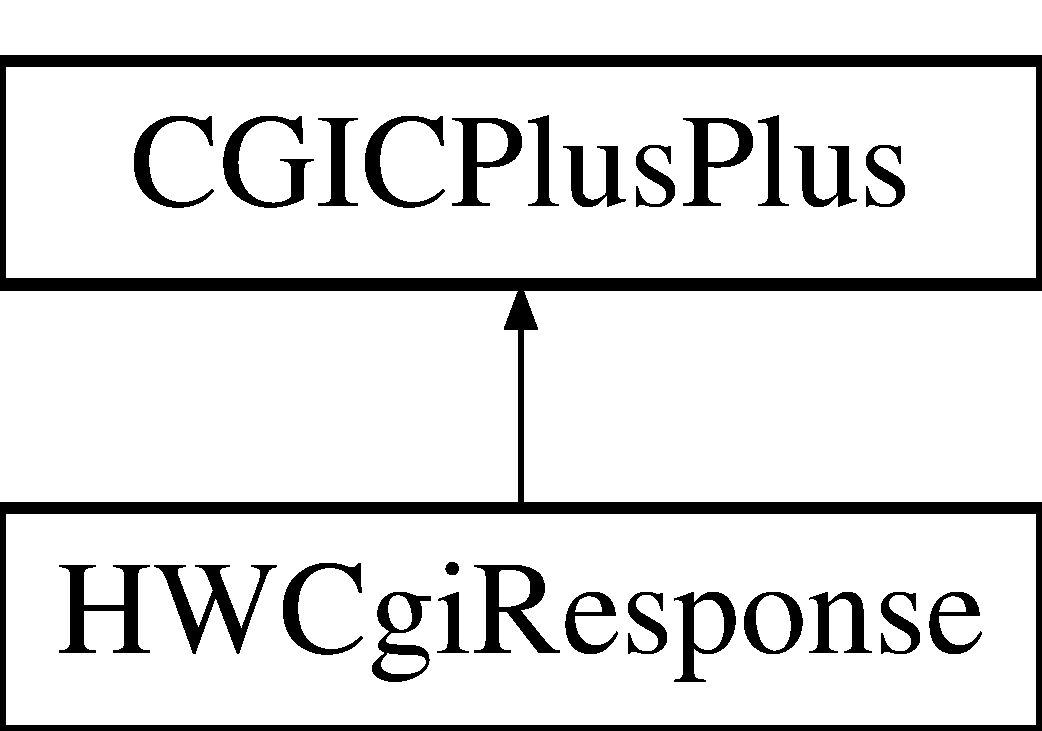
\includegraphics[height=2.000000cm]{class_h_w_cgi_response}
\end{center}
\end{figure}
\subsection*{\-Public \-Member \-Functions}
\begin{DoxyCompactItemize}
\item 
\hyperlink{class_h_w_cgi_response_a99da269334186fe6a7006fb679ad7dee}{\-H\-W\-Cgi\-Response} ()
\item 
virtual \hyperlink{class_h_w_cgi_response_a51edc5778a5af09fa39ce9fced0a221d}{$\sim$\-H\-W\-Cgi\-Response} ()
\item 
\hyperlink{_cpclient_8h_a6464f7480a0fd0ee170cba12b2c0497f}{void} \hyperlink{class_h_w_cgi_response_a1a4b4b8f0f682f9dc0a9e71dd6fa2fe5}{\-Process\-G\-E\-T\-Request} ()
\begin{DoxyCompactList}\small\item\em \-You must implement this method in a derived class. \end{DoxyCompactList}\item 
\hyperlink{_cpclient_8h_a6464f7480a0fd0ee170cba12b2c0497f}{void} \hyperlink{class_h_w_cgi_response_aec2b369683ddd63bad010575451aaec3}{\-Process\-P\-O\-S\-T\-Request} ()
\begin{DoxyCompactList}\small\item\em \-You must implement this method in a derived class. \end{DoxyCompactList}\end{DoxyCompactItemize}


\subsection{\-Detailed \-Description}


\-Definition at line 13 of file \-H\-W\-Cgi\-Response.\-h.



\subsection{\-Constructor \& \-Destructor \-Documentation}
\hypertarget{class_h_w_cgi_response_a99da269334186fe6a7006fb679ad7dee}{\index{\-H\-W\-Cgi\-Response@{\-H\-W\-Cgi\-Response}!\-H\-W\-Cgi\-Response@{\-H\-W\-Cgi\-Response}}
\index{\-H\-W\-Cgi\-Response@{\-H\-W\-Cgi\-Response}!HWCgiResponse@{\-H\-W\-Cgi\-Response}}
\subsubsection[{\-H\-W\-Cgi\-Response}]{\setlength{\rightskip}{0pt plus 5cm}{\bf \-H\-W\-Cgi\-Response\-::\-H\-W\-Cgi\-Response} (
\begin{DoxyParamCaption}
{}
\end{DoxyParamCaption}
)}}\label{class_h_w_cgi_response_a99da269334186fe6a7006fb679ad7dee}


\-Definition at line 10 of file \-H\-W\-Cgi\-Response.\-cpp.

\hypertarget{class_h_w_cgi_response_a51edc5778a5af09fa39ce9fced0a221d}{\index{\-H\-W\-Cgi\-Response@{\-H\-W\-Cgi\-Response}!$\sim$\-H\-W\-Cgi\-Response@{$\sim$\-H\-W\-Cgi\-Response}}
\index{$\sim$\-H\-W\-Cgi\-Response@{$\sim$\-H\-W\-Cgi\-Response}!HWCgiResponse@{\-H\-W\-Cgi\-Response}}
\subsubsection[{$\sim$\-H\-W\-Cgi\-Response}]{\setlength{\rightskip}{0pt plus 5cm}{\bf \-H\-W\-Cgi\-Response\-::$\sim$\-H\-W\-Cgi\-Response} (
\begin{DoxyParamCaption}
{}
\end{DoxyParamCaption}
)\hspace{0.3cm}{\ttfamily  \mbox{[}virtual\mbox{]}}}}\label{class_h_w_cgi_response_a51edc5778a5af09fa39ce9fced0a221d}


\-Definition at line 15 of file \-H\-W\-Cgi\-Response.\-cpp.



\subsection{\-Member \-Function \-Documentation}
\hypertarget{class_h_w_cgi_response_a1a4b4b8f0f682f9dc0a9e71dd6fa2fe5}{\index{\-H\-W\-Cgi\-Response@{\-H\-W\-Cgi\-Response}!\-Process\-G\-E\-T\-Request@{\-Process\-G\-E\-T\-Request}}
\index{\-Process\-G\-E\-T\-Request@{\-Process\-G\-E\-T\-Request}!HWCgiResponse@{\-H\-W\-Cgi\-Response}}
\subsubsection[{\-Process\-G\-E\-T\-Request}]{\setlength{\rightskip}{0pt plus 5cm}{\bf void} {\bf \-H\-W\-Cgi\-Response\-::\-Process\-G\-E\-T\-Request} (
\begin{DoxyParamCaption}
{}
\end{DoxyParamCaption}
)\hspace{0.3cm}{\ttfamily  \mbox{[}virtual\mbox{]}}}}\label{class_h_w_cgi_response_a1a4b4b8f0f682f9dc0a9e71dd6fa2fe5}


\-You must implement this method in a derived class. 



\-Reimplemented from \hyperlink{class_c_g_i_c_plus_plus_a378fb441bed59d816017d7e1ea6296f2}{\-C\-G\-I\-C\-Plus\-Plus}.



\-Definition at line 27 of file \-H\-W\-Cgi\-Response.\-cpp.

\hypertarget{class_h_w_cgi_response_aec2b369683ddd63bad010575451aaec3}{\index{\-H\-W\-Cgi\-Response@{\-H\-W\-Cgi\-Response}!\-Process\-P\-O\-S\-T\-Request@{\-Process\-P\-O\-S\-T\-Request}}
\index{\-Process\-P\-O\-S\-T\-Request@{\-Process\-P\-O\-S\-T\-Request}!HWCgiResponse@{\-H\-W\-Cgi\-Response}}
\subsubsection[{\-Process\-P\-O\-S\-T\-Request}]{\setlength{\rightskip}{0pt plus 5cm}{\bf void} {\bf \-H\-W\-Cgi\-Response\-::\-Process\-P\-O\-S\-T\-Request} (
\begin{DoxyParamCaption}
{}
\end{DoxyParamCaption}
)\hspace{0.3cm}{\ttfamily  \mbox{[}virtual\mbox{]}}}}\label{class_h_w_cgi_response_aec2b369683ddd63bad010575451aaec3}


\-You must implement this method in a derived class. 



\-Reimplemented from \hyperlink{class_c_g_i_c_plus_plus_a2f2776ae8909abdf3769c84415d64952}{\-C\-G\-I\-C\-Plus\-Plus}.



\-Definition at line 20 of file \-H\-W\-Cgi\-Response.\-cpp.



\-The documentation for this class was generated from the following files\-:\begin{DoxyCompactItemize}
\item 
common/examples/\-C\-G\-Iexample/\hyperlink{_h_w_cgi_response_8h}{\-H\-W\-Cgi\-Response.\-h}\item 
common/examples/\-C\-G\-Iexample/\hyperlink{_h_w_cgi_response_8cpp}{\-H\-W\-Cgi\-Response.\-cpp}\end{DoxyCompactItemize}

\hypertarget{structiphdr}{\section{iphdr \-Struct \-Reference}
\label{structiphdr}\index{iphdr@{iphdr}}
}


{\ttfamily \#include $<$icmp.\-h$>$}

\subsection*{\-Public \-Attributes}
\begin{DoxyCompactItemize}
\item 
unsigned char \hyperlink{structiphdr_a73f32935489a36a25baa9672f7e82cd0}{h\-\_\-len}\-:4
\item 
unsigned char \hyperlink{structiphdr_a232d177bba2eefdbab013bed9f8faf5d}{version}\-:4
\item 
unsigned char \hyperlink{structiphdr_a2efd9259c6f056707ceb0ae5bae5c90f}{tos}
\item 
unsigned short \hyperlink{structiphdr_abb34ffd5b3f3ea01b6981beda60359b6}{total\-\_\-len}
\item 
unsigned short \hyperlink{structiphdr_a5b9e10a88a5e925dd2fe53ad6e29e7a7}{ident}
\item 
unsigned short \hyperlink{structiphdr_a0d2e71cfe4d60b3fd494f89defd36403}{frag\-\_\-and\-\_\-flags}
\item 
unsigned char \hyperlink{structiphdr_acf6d9c663bfb22293ce2fadec78b7c9a}{ttl}
\item 
unsigned char \hyperlink{structiphdr_a8a39de7dc525754725363dc25fc75ae2}{proto}
\item 
unsigned short \hyperlink{structiphdr_ab16ea47d06f82b80994f3182b89fe26e}{checksum}
\item 
unsigned long \hyperlink{structiphdr_acb14e7dce69ddfa7895bb42c4268059e}{source\-I\-P}
\item 
unsigned long \hyperlink{structiphdr_a7131889c7b92b38bdeaac511bf7b6cc4}{dest\-I\-P}
\end{DoxyCompactItemize}


\subsection{\-Detailed \-Description}


\-Definition at line 84 of file icmp.\-h.



\subsection{\-Member \-Data \-Documentation}
\hypertarget{structiphdr_ab16ea47d06f82b80994f3182b89fe26e}{\index{iphdr@{iphdr}!checksum@{checksum}}
\index{checksum@{checksum}!iphdr@{iphdr}}
\subsubsection[{checksum}]{\setlength{\rightskip}{0pt plus 5cm}unsigned short {\bf iphdr\-::checksum}}}\label{structiphdr_ab16ea47d06f82b80994f3182b89fe26e}


\-Definition at line 102 of file icmp.\-h.

\hypertarget{structiphdr_a7131889c7b92b38bdeaac511bf7b6cc4}{\index{iphdr@{iphdr}!dest\-I\-P@{dest\-I\-P}}
\index{dest\-I\-P@{dest\-I\-P}!iphdr@{iphdr}}
\subsubsection[{dest\-I\-P}]{\setlength{\rightskip}{0pt plus 5cm}unsigned long {\bf iphdr\-::dest\-I\-P}}}\label{structiphdr_a7131889c7b92b38bdeaac511bf7b6cc4}


\-Definition at line 104 of file icmp.\-h.

\hypertarget{structiphdr_a0d2e71cfe4d60b3fd494f89defd36403}{\index{iphdr@{iphdr}!frag\-\_\-and\-\_\-flags@{frag\-\_\-and\-\_\-flags}}
\index{frag\-\_\-and\-\_\-flags@{frag\-\_\-and\-\_\-flags}!iphdr@{iphdr}}
\subsubsection[{frag\-\_\-and\-\_\-flags}]{\setlength{\rightskip}{0pt plus 5cm}unsigned short {\bf iphdr\-::frag\-\_\-and\-\_\-flags}}}\label{structiphdr_a0d2e71cfe4d60b3fd494f89defd36403}


\-Definition at line 99 of file icmp.\-h.

\hypertarget{structiphdr_a73f32935489a36a25baa9672f7e82cd0}{\index{iphdr@{iphdr}!h\-\_\-len@{h\-\_\-len}}
\index{h\-\_\-len@{h\-\_\-len}!iphdr@{iphdr}}
\subsubsection[{h\-\_\-len}]{\setlength{\rightskip}{0pt plus 5cm}unsigned char {\bf iphdr\-::h\-\_\-len}}}\label{structiphdr_a73f32935489a36a25baa9672f7e82cd0}


\-Definition at line 93 of file icmp.\-h.

\hypertarget{structiphdr_a5b9e10a88a5e925dd2fe53ad6e29e7a7}{\index{iphdr@{iphdr}!ident@{ident}}
\index{ident@{ident}!iphdr@{iphdr}}
\subsubsection[{ident}]{\setlength{\rightskip}{0pt plus 5cm}unsigned short {\bf iphdr\-::ident}}}\label{structiphdr_a5b9e10a88a5e925dd2fe53ad6e29e7a7}


\-Definition at line 98 of file icmp.\-h.

\hypertarget{structiphdr_a8a39de7dc525754725363dc25fc75ae2}{\index{iphdr@{iphdr}!proto@{proto}}
\index{proto@{proto}!iphdr@{iphdr}}
\subsubsection[{proto}]{\setlength{\rightskip}{0pt plus 5cm}unsigned char {\bf iphdr\-::proto}}}\label{structiphdr_a8a39de7dc525754725363dc25fc75ae2}


\-Definition at line 101 of file icmp.\-h.

\hypertarget{structiphdr_acb14e7dce69ddfa7895bb42c4268059e}{\index{iphdr@{iphdr}!source\-I\-P@{source\-I\-P}}
\index{source\-I\-P@{source\-I\-P}!iphdr@{iphdr}}
\subsubsection[{source\-I\-P}]{\setlength{\rightskip}{0pt plus 5cm}unsigned long {\bf iphdr\-::source\-I\-P}}}\label{structiphdr_acb14e7dce69ddfa7895bb42c4268059e}


\-Definition at line 103 of file icmp.\-h.

\hypertarget{structiphdr_a2efd9259c6f056707ceb0ae5bae5c90f}{\index{iphdr@{iphdr}!tos@{tos}}
\index{tos@{tos}!iphdr@{iphdr}}
\subsubsection[{tos}]{\setlength{\rightskip}{0pt plus 5cm}unsigned char {\bf iphdr\-::tos}}}\label{structiphdr_a2efd9259c6f056707ceb0ae5bae5c90f}


\-Definition at line 96 of file icmp.\-h.

\hypertarget{structiphdr_abb34ffd5b3f3ea01b6981beda60359b6}{\index{iphdr@{iphdr}!total\-\_\-len@{total\-\_\-len}}
\index{total\-\_\-len@{total\-\_\-len}!iphdr@{iphdr}}
\subsubsection[{total\-\_\-len}]{\setlength{\rightskip}{0pt plus 5cm}unsigned short {\bf iphdr\-::total\-\_\-len}}}\label{structiphdr_abb34ffd5b3f3ea01b6981beda60359b6}


\-Definition at line 97 of file icmp.\-h.

\hypertarget{structiphdr_acf6d9c663bfb22293ce2fadec78b7c9a}{\index{iphdr@{iphdr}!ttl@{ttl}}
\index{ttl@{ttl}!iphdr@{iphdr}}
\subsubsection[{ttl}]{\setlength{\rightskip}{0pt plus 5cm}unsigned char {\bf iphdr\-::ttl}}}\label{structiphdr_acf6d9c663bfb22293ce2fadec78b7c9a}


\-Definition at line 100 of file icmp.\-h.

\hypertarget{structiphdr_a232d177bba2eefdbab013bed9f8faf5d}{\index{iphdr@{iphdr}!version@{version}}
\index{version@{version}!iphdr@{iphdr}}
\subsubsection[{version}]{\setlength{\rightskip}{0pt plus 5cm}unsigned char {\bf iphdr\-::version}}}\label{structiphdr_a232d177bba2eefdbab013bed9f8faf5d}


\-Definition at line 94 of file icmp.\-h.



\-The documentation for this struct was generated from the following file\-:\begin{DoxyCompactItemize}
\item 
common/\hyperlink{icmp_8h}{icmp.\-h}\end{DoxyCompactItemize}

\chapter{\-File \-Documentation}
\hypertarget{_base64_coder_8cpp}{\section{common/\-Base64\-Coder.cpp \-File \-Reference}
\label{_base64_coder_8cpp}\index{common/\-Base64\-Coder.\-cpp@{common/\-Base64\-Coder.\-cpp}}
}
{\ttfamily \#include \char`\"{}\-Base64\-Coder.\-h\char`\"{}}\*
\subsection*{\-Defines}
\begin{DoxyCompactItemize}
\item 
\#define \hyperlink{_base64_coder_8cpp_a519adc2af3ba06a8f0548b6690050a89}{\-P\-A\-G\-E\-S\-I\-Z\-E}~4096
\item 
\#define \hyperlink{_base64_coder_8cpp_a5590a41d779003746329f12ebce4680c}{\-R\-O\-U\-N\-D\-T\-O\-P\-A\-G\-E}(a)~(((a/4096)+1)$\ast$4096)
\end{DoxyCompactItemize}


\subsection{\-Define \-Documentation}
\hypertarget{_base64_coder_8cpp_a519adc2af3ba06a8f0548b6690050a89}{\index{\-Base64\-Coder.\-cpp@{\-Base64\-Coder.\-cpp}!\-P\-A\-G\-E\-S\-I\-Z\-E@{\-P\-A\-G\-E\-S\-I\-Z\-E}}
\index{\-P\-A\-G\-E\-S\-I\-Z\-E@{\-P\-A\-G\-E\-S\-I\-Z\-E}!Base64Coder.cpp@{\-Base64\-Coder.\-cpp}}
\subsubsection[{\-P\-A\-G\-E\-S\-I\-Z\-E}]{\setlength{\rightskip}{0pt plus 5cm}\#define {\bf \-P\-A\-G\-E\-S\-I\-Z\-E}~4096}}\label{_base64_coder_8cpp_a519adc2af3ba06a8f0548b6690050a89}


\-Definition at line 31 of file \-Base64\-Coder.\-cpp.

\hypertarget{_base64_coder_8cpp_a5590a41d779003746329f12ebce4680c}{\index{\-Base64\-Coder.\-cpp@{\-Base64\-Coder.\-cpp}!\-R\-O\-U\-N\-D\-T\-O\-P\-A\-G\-E@{\-R\-O\-U\-N\-D\-T\-O\-P\-A\-G\-E}}
\index{\-R\-O\-U\-N\-D\-T\-O\-P\-A\-G\-E@{\-R\-O\-U\-N\-D\-T\-O\-P\-A\-G\-E}!Base64Coder.cpp@{\-Base64\-Coder.\-cpp}}
\subsubsection[{\-R\-O\-U\-N\-D\-T\-O\-P\-A\-G\-E}]{\setlength{\rightskip}{0pt plus 5cm}\#define {\bf \-R\-O\-U\-N\-D\-T\-O\-P\-A\-G\-E}(
\begin{DoxyParamCaption}
\item[{}]{a}
\end{DoxyParamCaption}
)~(((a/4096)+1)$\ast$4096)}}\label{_base64_coder_8cpp_a5590a41d779003746329f12ebce4680c}


\-Definition at line 35 of file \-Base64\-Coder.\-cpp.


\hypertarget{_base64_coder_8h}{\section{common/\-Base64\-Coder.h \-File \-Reference}
\label{_base64_coder_8h}\index{common/\-Base64\-Coder.\-h@{common/\-Base64\-Coder.\-h}}
}
{\ttfamily \#include \char`\"{}\-X\-Plat.\-h\char`\"{}}\*
\subsection*{\-Classes}
\begin{DoxyCompactItemize}
\item 
class \hyperlink{class_base64_coder}{\-Base64\-Coder}
\begin{DoxyCompactList}\small\item\em \hyperlink{_base64_coder_8h}{\-Base64\-Coder.\-h}\-: interface for the \hyperlink{class_base64_coder}{\-Base64\-Coder} class. \end{DoxyCompactList}\item 
class {\bfseries \-Base64\-Coder\-::\-Temp\-Bucket}
\begin{DoxyCompactList}\small\item\em \-Internal bucket class. \end{DoxyCompactList}\end{DoxyCompactItemize}

\hypertarget{_c_base_socket_8cpp}{\section{common/\-C\-Base\-Socket.cpp \-File \-Reference}
\label{_c_base_socket_8cpp}\index{common/\-C\-Base\-Socket.\-cpp@{common/\-C\-Base\-Socket.\-cpp}}
}
{\ttfamily \#include \char`\"{}\-X\-Plat.\-h\char`\"{}}\*
{\ttfamily \#include \char`\"{}\-C\-X\-Plat\-Thread.\-h\char`\"{}}\*
{\ttfamily \#include \char`\"{}\-C\-Base\-Socket.\-h\char`\"{}}\*

\hypertarget{_c_base_socket_8h}{\section{common/\-C\-Base\-Socket.h \-File \-Reference}
\label{_c_base_socket_8h}\index{common/\-C\-Base\-Socket.\-h@{common/\-C\-Base\-Socket.\-h}}
}
{\ttfamily \#include \char`\"{}\-X\-Plat.\-h\char`\"{}}\*
{\ttfamily \#include \char`\"{}\-C\-X\-Plat\-Critical\-Section.\-h\char`\"{}}\*
{\ttfamily \#include $<$sys/un.\-h$>$}\*
\subsection*{\-Classes}
\begin{DoxyCompactItemize}
\item 
class \hyperlink{class_c_base_socket}{\-C\-Base\-Socket}
\begin{DoxyCompactList}\small\item\em \-Base socket class implements low level \-Berkley socket functionality. \end{DoxyCompactList}\end{DoxyCompactItemize}
\subsection*{\-Defines}
\begin{DoxyCompactItemize}
\item 
\#define \hyperlink{_c_base_socket_8h_a8a11e53bc1742a507afb69fa92f17056}{\-K\-E\-R\-N\-E\-L\-\_\-2\-\_\-4}
\begin{DoxyCompactList}\small\item\em base class for socket \end{DoxyCompactList}\end{DoxyCompactItemize}


\subsection{\-Define \-Documentation}
\hypertarget{_c_base_socket_8h_a8a11e53bc1742a507afb69fa92f17056}{\index{\-C\-Base\-Socket.\-h@{\-C\-Base\-Socket.\-h}!\-K\-E\-R\-N\-E\-L\-\_\-2\-\_\-4@{\-K\-E\-R\-N\-E\-L\-\_\-2\-\_\-4}}
\index{\-K\-E\-R\-N\-E\-L\-\_\-2\-\_\-4@{\-K\-E\-R\-N\-E\-L\-\_\-2\-\_\-4}!CBaseSocket.h@{\-C\-Base\-Socket.\-h}}
\subsubsection[{\-K\-E\-R\-N\-E\-L\-\_\-2\-\_\-4}]{\setlength{\rightskip}{0pt plus 5cm}\#define {\bf \-K\-E\-R\-N\-E\-L\-\_\-2\-\_\-4}}}\label{_c_base_socket_8h_a8a11e53bc1742a507afb69fa92f17056}


base class for socket 



\-Definition at line 35 of file \-C\-Base\-Socket.\-h.


\hypertarget{_c_client_socket_8cpp}{\section{common/\-C\-Client\-Socket.cpp \-File \-Reference}
\label{_c_client_socket_8cpp}\index{common/\-C\-Client\-Socket.\-cpp@{common/\-C\-Client\-Socket.\-cpp}}
}
{\ttfamily \#include \char`\"{}\-X\-Plat.\-h\char`\"{}}\*
{\ttfamily \#include \char`\"{}\-C\-X\-Plat\-Thread.\-h\char`\"{}}\*
{\ttfamily \#include \char`\"{}\-C\-Base\-Socket.\-h\char`\"{}}\*
{\ttfamily \#include \char`\"{}\-C\-Connection\-Socket.\-h\char`\"{}}\*
{\ttfamily \#include \char`\"{}\-C\-Client\-Socket.\-h\char`\"{}}\*

\hypertarget{_c_client_socket_8h}{\section{common/\-C\-Client\-Socket.h \-File \-Reference}
\label{_c_client_socket_8h}\index{common/\-C\-Client\-Socket.\-h@{common/\-C\-Client\-Socket.\-h}}
}
{\ttfamily \#include \char`\"{}\-C\-X\-Plat\-Critical\-Section.\-h\char`\"{}}\*
{\ttfamily \#include \char`\"{}\-C\-X\-Plat\-Thread.\-h\char`\"{}}\*
{\ttfamily \#include \char`\"{}\-C\-X\-Plat\-Event.\-h\char`\"{}}\*
{\ttfamily \#include \char`\"{}\-C\-Connection\-Socket.\-h\char`\"{}}\*
\subsection*{\-Classes}
\begin{DoxyCompactItemize}
\item 
class \hyperlink{class_c_client_socket}{\-C\-Client\-Socket}
\begin{DoxyCompactList}\small\item\em \-Client socket. \end{DoxyCompactList}\end{DoxyCompactItemize}

\hypertarget{_c_connection_socket_8cpp}{\section{common/\-C\-Connection\-Socket.cpp \-File \-Reference}
\label{_c_connection_socket_8cpp}\index{common/\-C\-Connection\-Socket.\-cpp@{common/\-C\-Connection\-Socket.\-cpp}}
}
{\ttfamily \#include \char`\"{}\-X\-Plat.\-h\char`\"{}}\*
{\ttfamily \#include \char`\"{}\-C\-Base\-Socket.\-h\char`\"{}}\*
{\ttfamily \#include \char`\"{}\-C\-Connection\-Socket.\-h\char`\"{}}\*
{\ttfamily \#include $<$syslog.\-h$>$}\*
{\ttfamily \#include \char`\"{}\-C\-Profile\-Timer.\-h\char`\"{}}\*
{\ttfamily \#include $<$poll.\-h$>$}\*

\hypertarget{_c_connection_socket_8h}{\section{common/\-C\-Connection\-Socket.h \-File \-Reference}
\label{_c_connection_socket_8h}\index{common/\-C\-Connection\-Socket.\-h@{common/\-C\-Connection\-Socket.\-h}}
}
{\ttfamily \#include \char`\"{}\-C\-X\-Plat\-Thread.\-h\char`\"{}}\*
{\ttfamily \#include \char`\"{}\-C\-Base\-Socket.\-h\char`\"{}}\*
\subsection*{\-Classes}
\begin{DoxyCompactItemize}
\item 
class \hyperlink{class_c_connection_socket}{\-C\-Connection\-Socket}
\begin{DoxyCompactList}\small\item\em \hyperlink{class_c_connection_socket}{\-C\-Connection\-Socket} -\/ \-Establish a connection with the caller. \end{DoxyCompactList}\end{DoxyCompactItemize}

\hypertarget{_c_d_b_publisher_8cpp}{\section{common/\-C\-D\-B\-Publisher.cpp \-File \-Reference}
\label{_c_d_b_publisher_8cpp}\index{common/\-C\-D\-B\-Publisher.\-cpp@{common/\-C\-D\-B\-Publisher.\-cpp}}
}
{\ttfamily \#include \char`\"{}\-C\-D\-B\-Publisher.\-h\char`\"{}}\*
{\ttfamily \#include \char`\"{}\-C\-X\-Plat\-Event.\-h\char`\"{}}\*
{\ttfamily \#include $<$syslog.\-h$>$}\*
\subsection*{\-Variables}
\begin{DoxyCompactItemize}
\item 
const char $\ast$ \hyperlink{_c_d_b_publisher_8cpp_a57d0a3c474d2630a7de01f5d9af73803}{p\-Remove\-Start} = \char`\"{}\{'\%s' \-: \{\$in \-: \mbox{[}\char`\"{}
\item 
const char $\ast$ \hyperlink{_c_d_b_publisher_8cpp_a064a35a261b55b8189e147c58369c1ef}{p\-Remove\-End} = \char`\"{}\mbox{]}\}\}\char`\"{}
\end{DoxyCompactItemize}


\subsection{\-Variable \-Documentation}
\hypertarget{_c_d_b_publisher_8cpp_a064a35a261b55b8189e147c58369c1ef}{\index{\-C\-D\-B\-Publisher.\-cpp@{\-C\-D\-B\-Publisher.\-cpp}!p\-Remove\-End@{p\-Remove\-End}}
\index{p\-Remove\-End@{p\-Remove\-End}!CDBPublisher.cpp@{\-C\-D\-B\-Publisher.\-cpp}}
\subsubsection[{p\-Remove\-End}]{\setlength{\rightskip}{0pt plus 5cm}const char$\ast$ {\bf p\-Remove\-End} = \char`\"{}\mbox{]}\}\}\char`\"{}}}\label{_c_d_b_publisher_8cpp_a064a35a261b55b8189e147c58369c1ef}


\-Definition at line 24 of file \-C\-D\-B\-Publisher.\-cpp.

\hypertarget{_c_d_b_publisher_8cpp_a57d0a3c474d2630a7de01f5d9af73803}{\index{\-C\-D\-B\-Publisher.\-cpp@{\-C\-D\-B\-Publisher.\-cpp}!p\-Remove\-Start@{p\-Remove\-Start}}
\index{p\-Remove\-Start@{p\-Remove\-Start}!CDBPublisher.cpp@{\-C\-D\-B\-Publisher.\-cpp}}
\subsubsection[{p\-Remove\-Start}]{\setlength{\rightskip}{0pt plus 5cm}const char$\ast$ {\bf p\-Remove\-Start} = \char`\"{}\{'\%s' \-: \{\$in \-: \mbox{[}\char`\"{}}}\label{_c_d_b_publisher_8cpp_a57d0a3c474d2630a7de01f5d9af73803}


\-Definition at line 23 of file \-C\-D\-B\-Publisher.\-cpp.


\hypertarget{_c_d_b_publisher_8h}{\section{common/\-C\-D\-B\-Publisher.h \-File \-Reference}
\label{_c_d_b_publisher_8h}\index{common/\-C\-D\-B\-Publisher.\-h@{common/\-C\-D\-B\-Publisher.\-h}}
}
{\ttfamily \#include \char`\"{}\-C\-X\-Plat\-Thread.\-h\char`\"{}}\*
{\ttfamily \#include \char`\"{}\-C\-X\-Plat\-Event.\-h\char`\"{}}\*
{\ttfamily \#include \char`\"{}\-C\-D\-B\-Records\-Array.\-h\char`\"{}}\*
{\ttfamily \#include $<$mongo/client/dbclient.\-h$>$}\*
\subsection*{\-Classes}
\begin{DoxyCompactItemize}
\item 
class \hyperlink{class_d_b_stats}{\-D\-B\-Stats}
\begin{DoxyCompactList}\small\item\em \-Class \hyperlink{class_d_b_stats}{\-D\-B\-Stats} keeps track of \-D\-B statistics. \end{DoxyCompactList}\item 
class \hyperlink{class_c_d_b_publisher}{\-C\-D\-B\-Publisher}
\end{DoxyCompactItemize}
\subsection*{\-Defines}
\begin{DoxyCompactItemize}
\item 
\#define \hyperlink{_c_d_b_publisher_8h_a4663229004d120a06c202e46db5d2d4d}{\-V\-E\-C\-\_\-\-D\-B\-\_\-\-K\-E\-Y\-S}~\hyperlink{_c_d_b_records_array_8h_a32e3940d41c32d8e161b8775f6c4296a}{\-V\-E\-C\-\_\-\-D\-B\-\_\-\-R\-E\-C\-O\-R\-D\-S}
\end{DoxyCompactItemize}


\subsection{\-Define \-Documentation}
\hypertarget{_c_d_b_publisher_8h_a4663229004d120a06c202e46db5d2d4d}{\index{\-C\-D\-B\-Publisher.\-h@{\-C\-D\-B\-Publisher.\-h}!\-V\-E\-C\-\_\-\-D\-B\-\_\-\-K\-E\-Y\-S@{\-V\-E\-C\-\_\-\-D\-B\-\_\-\-K\-E\-Y\-S}}
\index{\-V\-E\-C\-\_\-\-D\-B\-\_\-\-K\-E\-Y\-S@{\-V\-E\-C\-\_\-\-D\-B\-\_\-\-K\-E\-Y\-S}!CDBPublisher.h@{\-C\-D\-B\-Publisher.\-h}}
\subsubsection[{\-V\-E\-C\-\_\-\-D\-B\-\_\-\-K\-E\-Y\-S}]{\setlength{\rightskip}{0pt plus 5cm}\#define {\bf \-V\-E\-C\-\_\-\-D\-B\-\_\-\-K\-E\-Y\-S}~{\bf \-V\-E\-C\-\_\-\-D\-B\-\_\-\-R\-E\-C\-O\-R\-D\-S}}}\label{_c_d_b_publisher_8h_a4663229004d120a06c202e46db5d2d4d}


\-Definition at line 28 of file \-C\-D\-B\-Publisher.\-h.


\hypertarget{_c_d_b_records_array_8cpp}{\section{common/\-C\-D\-B\-Records\-Array.cpp \-File \-Reference}
\label{_c_d_b_records_array_8cpp}\index{common/\-C\-D\-B\-Records\-Array.\-cpp@{common/\-C\-D\-B\-Records\-Array.\-cpp}}
}
{\ttfamily \#include \char`\"{}\-C\-D\-B\-Records\-Array.\-h\char`\"{}}\*

\hypertarget{_c_d_b_records_array_8h}{\section{common/\-C\-D\-B\-Records\-Array.h \-File \-Reference}
\label{_c_d_b_records_array_8h}\index{common/\-C\-D\-B\-Records\-Array.\-h@{common/\-C\-D\-B\-Records\-Array.\-h}}
}
{\ttfamily \#include $<$map$>$}\*
{\ttfamily \#include $<$string$>$}\*
{\ttfamily \#include \char`\"{}\-C\-X\-Plat\-Critical\-Section.\-h\char`\"{}}\*
\subsection*{\-Classes}
\begin{DoxyCompactItemize}
\item 
class \hyperlink{class_c_d_b_records_array}{\-C\-D\-B\-Records\-Array}
\end{DoxyCompactItemize}
\subsection*{\-Typedefs}
\begin{DoxyCompactItemize}
\item 
typedef vector$<$ string $>$ \hyperlink{_c_d_b_records_array_8h_a32e3940d41c32d8e161b8775f6c4296a}{\-V\-E\-C\-\_\-\-D\-B\-\_\-\-R\-E\-C\-O\-R\-D\-S}
\end{DoxyCompactItemize}


\subsection{\-Typedef \-Documentation}
\hypertarget{_c_d_b_records_array_8h_a32e3940d41c32d8e161b8775f6c4296a}{\index{\-C\-D\-B\-Records\-Array.\-h@{\-C\-D\-B\-Records\-Array.\-h}!\-V\-E\-C\-\_\-\-D\-B\-\_\-\-R\-E\-C\-O\-R\-D\-S@{\-V\-E\-C\-\_\-\-D\-B\-\_\-\-R\-E\-C\-O\-R\-D\-S}}
\index{\-V\-E\-C\-\_\-\-D\-B\-\_\-\-R\-E\-C\-O\-R\-D\-S@{\-V\-E\-C\-\_\-\-D\-B\-\_\-\-R\-E\-C\-O\-R\-D\-S}!CDBRecordsArray.h@{\-C\-D\-B\-Records\-Array.\-h}}
\subsubsection[{\-V\-E\-C\-\_\-\-D\-B\-\_\-\-R\-E\-C\-O\-R\-D\-S}]{\setlength{\rightskip}{0pt plus 5cm}typedef vector$<$string$>$ {\bf \-V\-E\-C\-\_\-\-D\-B\-\_\-\-R\-E\-C\-O\-R\-D\-S}}}\label{_c_d_b_records_array_8h_a32e3940d41c32d8e161b8775f6c4296a}


\-Definition at line 28 of file \-C\-D\-B\-Records\-Array.\-h.


\hypertarget{_c_explode_8cpp}{\section{common/\-C\-Explode.cpp \-File \-Reference}
\label{_c_explode_8cpp}\index{common/\-C\-Explode.\-cpp@{common/\-C\-Explode.\-cpp}}
}
{\ttfamily \#include \char`\"{}\-C\-Explode.\-h\char`\"{}}\*
{\ttfamily \#include \char`\"{}string.\-h\char`\"{}}\*

\hypertarget{_c_explode_8h}{\section{common/\-C\-Explode.h \-File \-Reference}
\label{_c_explode_8h}\index{common/\-C\-Explode.\-h@{common/\-C\-Explode.\-h}}
}
{\ttfamily \#include $<$vector$>$}\*
{\ttfamily \#include $<$string$>$}\*
\subsection*{\-Classes}
\begin{DoxyCompactItemize}
\item 
class \hyperlink{class_c_explode}{\-C\-Explode}
\begin{DoxyCompactList}\small\item\em \hyperlink{class_c_explode}{\-C\-Explode} -\/ similar to \-P\-H\-P's \char`\"{}explode\char`\"{} function. \end{DoxyCompactList}\end{DoxyCompactItemize}
\subsection*{\-Typedefs}
\begin{DoxyCompactItemize}
\item 
typedef vector$<$ string $>$ \hyperlink{_c_explode_8h_aa2caa24be48f42e10b14d8e285ad4de0}{\-V\-E\-C\-T\-O\-R\-\_\-\-P\-H\-R\-A\-S\-E\-S}
\end{DoxyCompactItemize}


\subsection{\-Typedef \-Documentation}
\hypertarget{_c_explode_8h_aa2caa24be48f42e10b14d8e285ad4de0}{\index{\-C\-Explode.\-h@{\-C\-Explode.\-h}!\-V\-E\-C\-T\-O\-R\-\_\-\-P\-H\-R\-A\-S\-E\-S@{\-V\-E\-C\-T\-O\-R\-\_\-\-P\-H\-R\-A\-S\-E\-S}}
\index{\-V\-E\-C\-T\-O\-R\-\_\-\-P\-H\-R\-A\-S\-E\-S@{\-V\-E\-C\-T\-O\-R\-\_\-\-P\-H\-R\-A\-S\-E\-S}!CExplode.h@{\-C\-Explode.\-h}}
\subsubsection[{\-V\-E\-C\-T\-O\-R\-\_\-\-P\-H\-R\-A\-S\-E\-S}]{\setlength{\rightskip}{0pt plus 5cm}typedef vector$<$string$>$ {\bf \-V\-E\-C\-T\-O\-R\-\_\-\-P\-H\-R\-A\-S\-E\-S}}}\label{_c_explode_8h_aa2caa24be48f42e10b14d8e285ad4de0}


\-Definition at line 31 of file \-C\-Explode.\-h.


\hypertarget{_c_flush_log_thread_8cpp}{\section{common/\-C\-Flush\-Log\-Thread.cpp \-File \-Reference}
\label{_c_flush_log_thread_8cpp}\index{common/\-C\-Flush\-Log\-Thread.\-cpp@{common/\-C\-Flush\-Log\-Thread.\-cpp}}
}
{\ttfamily \#include \char`\"{}\-X\-Plat.\-h\char`\"{}}\*
{\ttfamily \#include \char`\"{}\-C\-Flush\-Log\-Thread.\-h\char`\"{}}\*
{\ttfamily \#include \char`\"{}\-C\-Logging.\-h\char`\"{}}\*

\hypertarget{_c_flush_log_thread_8h}{\section{common/\-C\-Flush\-Log\-Thread.h \-File \-Reference}
\label{_c_flush_log_thread_8h}\index{common/\-C\-Flush\-Log\-Thread.\-h@{common/\-C\-Flush\-Log\-Thread.\-h}}
}
{\ttfamily \#include \char`\"{}\-C\-X\-Plat\-Thread.\-h\char`\"{}}\*
{\ttfamily \#include \char`\"{}\-C\-X\-Plat\-Event.\-h\char`\"{}}\*
\subsection*{\-Classes}
\begin{DoxyCompactItemize}
\item 
class \hyperlink{class_c_flush_log_thread}{\-C\-Flush\-Log\-Thread}
\begin{DoxyCompactList}\small\item\em \hyperlink{_c_flush_log_thread_8h}{\-C\-Flush\-Log\-Thread.\-h}\-: interface for the \hyperlink{class_c_flush_log_thread}{\-C\-Flush\-Log\-Thread} class. \end{DoxyCompactList}\end{DoxyCompactItemize}

\hypertarget{_c_g_i_c_plus_plus_8cpp}{\section{common/\-C\-G\-I\-C\-Plus\-Plus.cpp \-File \-Reference}
\label{_c_g_i_c_plus_plus_8cpp}\index{common/\-C\-G\-I\-C\-Plus\-Plus.\-cpp@{common/\-C\-G\-I\-C\-Plus\-Plus.\-cpp}}
}
{\ttfamily \#include \char`\"{}\-C\-G\-I\-C\-Plus\-Plus.\-h\char`\"{}}\*

\hypertarget{examples_2_c_g_iexample_2_c_g_i_c_plus_plus_8cpp}{\section{common/examples/\-C\-G\-Iexample/\-C\-G\-I\-C\-Plus\-Plus.cpp \-File \-Reference}
\label{examples_2_c_g_iexample_2_c_g_i_c_plus_plus_8cpp}\index{common/examples/\-C\-G\-Iexample/\-C\-G\-I\-C\-Plus\-Plus.\-cpp@{common/examples/\-C\-G\-Iexample/\-C\-G\-I\-C\-Plus\-Plus.\-cpp}}
}
{\ttfamily \#include \char`\"{}\-C\-G\-I\-C\-Plus\-Plus.\-h\char`\"{}}\*

\hypertarget{_c_g_i_c_plus_plus_8h}{\section{common/\-C\-G\-I\-C\-Plus\-Plus.h \-File \-Reference}
\label{_c_g_i_c_plus_plus_8h}\index{common/\-C\-G\-I\-C\-Plus\-Plus.\-h@{common/\-C\-G\-I\-C\-Plus\-Plus.\-h}}
}
{\ttfamily \#include $<$stdio.\-h$>$}\*
{\ttfamily \#include $<$string.\-h$>$}\*
{\ttfamily \#include $<$stdlib.\-h$>$}\*
{\ttfamily \#include $<$unistd.\-h$>$}\*
{\ttfamily \#include $<$map$>$}\*
{\ttfamily \#include $<$string$>$}\*
\subsection*{\-Classes}
\begin{DoxyCompactItemize}
\item 
class \hyperlink{class_c_g_i_c_plus_plus}{\-C\-G\-I\-C\-Plus\-Plus}
\begin{DoxyCompactList}\small\item\em \-Wrapper to simplify \-C++ creation of \-C\-G\-I programs. \end{DoxyCompactList}\end{DoxyCompactItemize}
\subsection*{\-Defines}
\begin{DoxyCompactItemize}
\item 
\#define \hyperlink{_c_g_i_c_plus_plus_8h_ae0a87e02cbaeb5dc5521343b862a4956}{\-M\-I\-M\-E\-\_\-\-H\-T\-M\-L}~\char`\"{}text/html\char`\"{}
\item 
\#define \hyperlink{_c_g_i_c_plus_plus_8h_ad6c1c77b6e5a5ca529e33608798eb34f}{\-M\-I\-M\-E\-\_\-\-X\-M\-L}~\char`\"{}text/xml\char`\"{}
\item 
\#define \hyperlink{_c_g_i_c_plus_plus_8h_a0aee6601ce17bab561fb47546e795a3f}{\-C\-O\-N\-T\-E\-N\-T\-\_\-\-F\-O\-R\-M}~\char`\"{}application/x-\/www-\/form-\/urlencoded\char`\"{}
\item 
\#define \hyperlink{_c_g_i_c_plus_plus_8h_ae56fdb340b23940f7a64ed2e37c1774a}{\-S\-T\-A\-T\-U\-S\-\_\-\-S\-U\-C\-C\-E\-S\-S}~\char`\"{}\-Status\-: 200 success\char`\"{}
\item 
\#define \hyperlink{_c_g_i_c_plus_plus_8h_a5300f78efbf158dfba0a0f3854065ca9}{\-S\-T\-A\-T\-U\-S\-\_\-\-I\-N\-V\-A\-L\-I\-D\-\_\-\-R\-E\-Q\-U\-E\-S\-T}~\char`\"{}\-Status\-: 400 invalid request\char`\"{}
\item 
\#define \hyperlink{_c_g_i_c_plus_plus_8h_ac345972a587e6779b3c5d40874080e51}{\-S\-T\-A\-T\-U\-S\-\_\-\-N\-O\-T\-\_\-\-F\-O\-U\-N\-D}~\char`\"{}\-Status\-: 404 not found\char`\"{}
\item 
\#define \hyperlink{_c_g_i_c_plus_plus_8h_a5300f78efbf158dfba0a0f3854065ca9}{\-S\-T\-A\-T\-U\-S\-\_\-\-I\-N\-V\-A\-L\-I\-D\-\_\-\-R\-E\-Q\-U\-E\-S\-T}~\char`\"{}\-Status\-: 400 invalid request\char`\"{}
\item 
\#define \hyperlink{_c_g_i_c_plus_plus_8h_ae4a97f0d170bc8dc771aac6c4f38ad1d}{\-S\-T\-A\-T\-U\-S\-\_\-\-E\-R\-R\-O\-R}~\char`\"{}\-Status\-: 500 web service error\char`\"{}
\end{DoxyCompactItemize}
\subsection*{\-Typedefs}
\begin{DoxyCompactItemize}
\item 
typedef map$<$ string, string $>$ \hyperlink{_c_g_i_c_plus_plus_8h_a4dec09a80640f7bd2995d58d468076c8}{\-M\-A\-P\-\_\-\-C\-G\-I\-\_\-\-V\-A\-L\-U\-E\-S}
\item 
typedef \-M\-A\-P\-\_\-\-C\-G\-I\-\_\-\-V\-A\-L\-U\-E\-S\-::iterator \hyperlink{_c_g_i_c_plus_plus_8h_af7e8a42feb278a380f7c0926876e028d}{\-C\-V\-Iter}
\end{DoxyCompactItemize}


\subsection{\-Define \-Documentation}
\hypertarget{_c_g_i_c_plus_plus_8h_a0aee6601ce17bab561fb47546e795a3f}{\index{\-C\-G\-I\-C\-Plus\-Plus.\-h@{\-C\-G\-I\-C\-Plus\-Plus.\-h}!\-C\-O\-N\-T\-E\-N\-T\-\_\-\-F\-O\-R\-M@{\-C\-O\-N\-T\-E\-N\-T\-\_\-\-F\-O\-R\-M}}
\index{\-C\-O\-N\-T\-E\-N\-T\-\_\-\-F\-O\-R\-M@{\-C\-O\-N\-T\-E\-N\-T\-\_\-\-F\-O\-R\-M}!CGICPlusPlus.h@{\-C\-G\-I\-C\-Plus\-Plus.\-h}}
\subsubsection[{\-C\-O\-N\-T\-E\-N\-T\-\_\-\-F\-O\-R\-M}]{\setlength{\rightskip}{0pt plus 5cm}\#define {\bf \-C\-O\-N\-T\-E\-N\-T\-\_\-\-F\-O\-R\-M}~\char`\"{}application/x-\/www-\/form-\/urlencoded\char`\"{}}}\label{_c_g_i_c_plus_plus_8h_a0aee6601ce17bab561fb47546e795a3f}


\-Definition at line 35 of file \-C\-G\-I\-C\-Plus\-Plus.\-h.

\hypertarget{_c_g_i_c_plus_plus_8h_ae0a87e02cbaeb5dc5521343b862a4956}{\index{\-C\-G\-I\-C\-Plus\-Plus.\-h@{\-C\-G\-I\-C\-Plus\-Plus.\-h}!\-M\-I\-M\-E\-\_\-\-H\-T\-M\-L@{\-M\-I\-M\-E\-\_\-\-H\-T\-M\-L}}
\index{\-M\-I\-M\-E\-\_\-\-H\-T\-M\-L@{\-M\-I\-M\-E\-\_\-\-H\-T\-M\-L}!CGICPlusPlus.h@{\-C\-G\-I\-C\-Plus\-Plus.\-h}}
\subsubsection[{\-M\-I\-M\-E\-\_\-\-H\-T\-M\-L}]{\setlength{\rightskip}{0pt plus 5cm}\#define {\bf \-M\-I\-M\-E\-\_\-\-H\-T\-M\-L}~\char`\"{}text/html\char`\"{}}}\label{_c_g_i_c_plus_plus_8h_ae0a87e02cbaeb5dc5521343b862a4956}


\-Definition at line 33 of file \-C\-G\-I\-C\-Plus\-Plus.\-h.

\hypertarget{_c_g_i_c_plus_plus_8h_ad6c1c77b6e5a5ca529e33608798eb34f}{\index{\-C\-G\-I\-C\-Plus\-Plus.\-h@{\-C\-G\-I\-C\-Plus\-Plus.\-h}!\-M\-I\-M\-E\-\_\-\-X\-M\-L@{\-M\-I\-M\-E\-\_\-\-X\-M\-L}}
\index{\-M\-I\-M\-E\-\_\-\-X\-M\-L@{\-M\-I\-M\-E\-\_\-\-X\-M\-L}!CGICPlusPlus.h@{\-C\-G\-I\-C\-Plus\-Plus.\-h}}
\subsubsection[{\-M\-I\-M\-E\-\_\-\-X\-M\-L}]{\setlength{\rightskip}{0pt plus 5cm}\#define {\bf \-M\-I\-M\-E\-\_\-\-X\-M\-L}~\char`\"{}text/xml\char`\"{}}}\label{_c_g_i_c_plus_plus_8h_ad6c1c77b6e5a5ca529e33608798eb34f}


\-Definition at line 34 of file \-C\-G\-I\-C\-Plus\-Plus.\-h.

\hypertarget{_c_g_i_c_plus_plus_8h_ae4a97f0d170bc8dc771aac6c4f38ad1d}{\index{\-C\-G\-I\-C\-Plus\-Plus.\-h@{\-C\-G\-I\-C\-Plus\-Plus.\-h}!\-S\-T\-A\-T\-U\-S\-\_\-\-E\-R\-R\-O\-R@{\-S\-T\-A\-T\-U\-S\-\_\-\-E\-R\-R\-O\-R}}
\index{\-S\-T\-A\-T\-U\-S\-\_\-\-E\-R\-R\-O\-R@{\-S\-T\-A\-T\-U\-S\-\_\-\-E\-R\-R\-O\-R}!CGICPlusPlus.h@{\-C\-G\-I\-C\-Plus\-Plus.\-h}}
\subsubsection[{\-S\-T\-A\-T\-U\-S\-\_\-\-E\-R\-R\-O\-R}]{\setlength{\rightskip}{0pt plus 5cm}\#define {\bf \-S\-T\-A\-T\-U\-S\-\_\-\-E\-R\-R\-O\-R}~\char`\"{}\-Status\-: 500 web service error\char`\"{}}}\label{_c_g_i_c_plus_plus_8h_ae4a97f0d170bc8dc771aac6c4f38ad1d}


\-Definition at line 40 of file \-C\-G\-I\-C\-Plus\-Plus.\-h.

\hypertarget{_c_g_i_c_plus_plus_8h_a5300f78efbf158dfba0a0f3854065ca9}{\index{\-C\-G\-I\-C\-Plus\-Plus.\-h@{\-C\-G\-I\-C\-Plus\-Plus.\-h}!\-S\-T\-A\-T\-U\-S\-\_\-\-I\-N\-V\-A\-L\-I\-D\-\_\-\-R\-E\-Q\-U\-E\-S\-T@{\-S\-T\-A\-T\-U\-S\-\_\-\-I\-N\-V\-A\-L\-I\-D\-\_\-\-R\-E\-Q\-U\-E\-S\-T}}
\index{\-S\-T\-A\-T\-U\-S\-\_\-\-I\-N\-V\-A\-L\-I\-D\-\_\-\-R\-E\-Q\-U\-E\-S\-T@{\-S\-T\-A\-T\-U\-S\-\_\-\-I\-N\-V\-A\-L\-I\-D\-\_\-\-R\-E\-Q\-U\-E\-S\-T}!CGICPlusPlus.h@{\-C\-G\-I\-C\-Plus\-Plus.\-h}}
\subsubsection[{\-S\-T\-A\-T\-U\-S\-\_\-\-I\-N\-V\-A\-L\-I\-D\-\_\-\-R\-E\-Q\-U\-E\-S\-T}]{\setlength{\rightskip}{0pt plus 5cm}\#define {\bf \-S\-T\-A\-T\-U\-S\-\_\-\-I\-N\-V\-A\-L\-I\-D\-\_\-\-R\-E\-Q\-U\-E\-S\-T}~\char`\"{}\-Status\-: 400 invalid request\char`\"{}}}\label{_c_g_i_c_plus_plus_8h_a5300f78efbf158dfba0a0f3854065ca9}


\-Definition at line 39 of file \-C\-G\-I\-C\-Plus\-Plus.\-h.

\hypertarget{_c_g_i_c_plus_plus_8h_a5300f78efbf158dfba0a0f3854065ca9}{\index{\-C\-G\-I\-C\-Plus\-Plus.\-h@{\-C\-G\-I\-C\-Plus\-Plus.\-h}!\-S\-T\-A\-T\-U\-S\-\_\-\-I\-N\-V\-A\-L\-I\-D\-\_\-\-R\-E\-Q\-U\-E\-S\-T@{\-S\-T\-A\-T\-U\-S\-\_\-\-I\-N\-V\-A\-L\-I\-D\-\_\-\-R\-E\-Q\-U\-E\-S\-T}}
\index{\-S\-T\-A\-T\-U\-S\-\_\-\-I\-N\-V\-A\-L\-I\-D\-\_\-\-R\-E\-Q\-U\-E\-S\-T@{\-S\-T\-A\-T\-U\-S\-\_\-\-I\-N\-V\-A\-L\-I\-D\-\_\-\-R\-E\-Q\-U\-E\-S\-T}!CGICPlusPlus.h@{\-C\-G\-I\-C\-Plus\-Plus.\-h}}
\subsubsection[{\-S\-T\-A\-T\-U\-S\-\_\-\-I\-N\-V\-A\-L\-I\-D\-\_\-\-R\-E\-Q\-U\-E\-S\-T}]{\setlength{\rightskip}{0pt plus 5cm}\#define {\bf \-S\-T\-A\-T\-U\-S\-\_\-\-I\-N\-V\-A\-L\-I\-D\-\_\-\-R\-E\-Q\-U\-E\-S\-T}~\char`\"{}\-Status\-: 400 invalid request\char`\"{}}}\label{_c_g_i_c_plus_plus_8h_a5300f78efbf158dfba0a0f3854065ca9}


\-Definition at line 39 of file \-C\-G\-I\-C\-Plus\-Plus.\-h.

\hypertarget{_c_g_i_c_plus_plus_8h_ac345972a587e6779b3c5d40874080e51}{\index{\-C\-G\-I\-C\-Plus\-Plus.\-h@{\-C\-G\-I\-C\-Plus\-Plus.\-h}!\-S\-T\-A\-T\-U\-S\-\_\-\-N\-O\-T\-\_\-\-F\-O\-U\-N\-D@{\-S\-T\-A\-T\-U\-S\-\_\-\-N\-O\-T\-\_\-\-F\-O\-U\-N\-D}}
\index{\-S\-T\-A\-T\-U\-S\-\_\-\-N\-O\-T\-\_\-\-F\-O\-U\-N\-D@{\-S\-T\-A\-T\-U\-S\-\_\-\-N\-O\-T\-\_\-\-F\-O\-U\-N\-D}!CGICPlusPlus.h@{\-C\-G\-I\-C\-Plus\-Plus.\-h}}
\subsubsection[{\-S\-T\-A\-T\-U\-S\-\_\-\-N\-O\-T\-\_\-\-F\-O\-U\-N\-D}]{\setlength{\rightskip}{0pt plus 5cm}\#define {\bf \-S\-T\-A\-T\-U\-S\-\_\-\-N\-O\-T\-\_\-\-F\-O\-U\-N\-D}~\char`\"{}\-Status\-: 404 not found\char`\"{}}}\label{_c_g_i_c_plus_plus_8h_ac345972a587e6779b3c5d40874080e51}


\-Definition at line 38 of file \-C\-G\-I\-C\-Plus\-Plus.\-h.

\hypertarget{_c_g_i_c_plus_plus_8h_ae56fdb340b23940f7a64ed2e37c1774a}{\index{\-C\-G\-I\-C\-Plus\-Plus.\-h@{\-C\-G\-I\-C\-Plus\-Plus.\-h}!\-S\-T\-A\-T\-U\-S\-\_\-\-S\-U\-C\-C\-E\-S\-S@{\-S\-T\-A\-T\-U\-S\-\_\-\-S\-U\-C\-C\-E\-S\-S}}
\index{\-S\-T\-A\-T\-U\-S\-\_\-\-S\-U\-C\-C\-E\-S\-S@{\-S\-T\-A\-T\-U\-S\-\_\-\-S\-U\-C\-C\-E\-S\-S}!CGICPlusPlus.h@{\-C\-G\-I\-C\-Plus\-Plus.\-h}}
\subsubsection[{\-S\-T\-A\-T\-U\-S\-\_\-\-S\-U\-C\-C\-E\-S\-S}]{\setlength{\rightskip}{0pt plus 5cm}\#define {\bf \-S\-T\-A\-T\-U\-S\-\_\-\-S\-U\-C\-C\-E\-S\-S}~\char`\"{}\-Status\-: 200 success\char`\"{}}}\label{_c_g_i_c_plus_plus_8h_ae56fdb340b23940f7a64ed2e37c1774a}


\-Definition at line 36 of file \-C\-G\-I\-C\-Plus\-Plus.\-h.



\subsection{\-Typedef \-Documentation}
\hypertarget{_c_g_i_c_plus_plus_8h_af7e8a42feb278a380f7c0926876e028d}{\index{\-C\-G\-I\-C\-Plus\-Plus.\-h@{\-C\-G\-I\-C\-Plus\-Plus.\-h}!\-C\-V\-Iter@{\-C\-V\-Iter}}
\index{\-C\-V\-Iter@{\-C\-V\-Iter}!CGICPlusPlus.h@{\-C\-G\-I\-C\-Plus\-Plus.\-h}}
\subsubsection[{\-C\-V\-Iter}]{\setlength{\rightskip}{0pt plus 5cm}typedef \-M\-A\-P\-\_\-\-C\-G\-I\-\_\-\-V\-A\-L\-U\-E\-S\-::iterator {\bf \-C\-V\-Iter}}}\label{_c_g_i_c_plus_plus_8h_af7e8a42feb278a380f7c0926876e028d}


\-Definition at line 45 of file \-C\-G\-I\-C\-Plus\-Plus.\-h.

\hypertarget{_c_g_i_c_plus_plus_8h_a4dec09a80640f7bd2995d58d468076c8}{\index{\-C\-G\-I\-C\-Plus\-Plus.\-h@{\-C\-G\-I\-C\-Plus\-Plus.\-h}!\-M\-A\-P\-\_\-\-C\-G\-I\-\_\-\-V\-A\-L\-U\-E\-S@{\-M\-A\-P\-\_\-\-C\-G\-I\-\_\-\-V\-A\-L\-U\-E\-S}}
\index{\-M\-A\-P\-\_\-\-C\-G\-I\-\_\-\-V\-A\-L\-U\-E\-S@{\-M\-A\-P\-\_\-\-C\-G\-I\-\_\-\-V\-A\-L\-U\-E\-S}!CGICPlusPlus.h@{\-C\-G\-I\-C\-Plus\-Plus.\-h}}
\subsubsection[{\-M\-A\-P\-\_\-\-C\-G\-I\-\_\-\-V\-A\-L\-U\-E\-S}]{\setlength{\rightskip}{0pt plus 5cm}typedef map$<$string, string$>$ {\bf \-M\-A\-P\-\_\-\-C\-G\-I\-\_\-\-V\-A\-L\-U\-E\-S}}}\label{_c_g_i_c_plus_plus_8h_a4dec09a80640f7bd2995d58d468076c8}


\-Definition at line 44 of file \-C\-G\-I\-C\-Plus\-Plus.\-h.


\hypertarget{examples_2_c_g_iexample_2_c_g_i_c_plus_plus_8h}{\section{common/examples/\-C\-G\-Iexample/\-C\-G\-I\-C\-Plus\-Plus.h \-File \-Reference}
\label{examples_2_c_g_iexample_2_c_g_i_c_plus_plus_8h}\index{common/examples/\-C\-G\-Iexample/\-C\-G\-I\-C\-Plus\-Plus.\-h@{common/examples/\-C\-G\-Iexample/\-C\-G\-I\-C\-Plus\-Plus.\-h}}
}
{\ttfamily \#include $<$stdio.\-h$>$}\*
{\ttfamily \#include $<$string.\-h$>$}\*
{\ttfamily \#include $<$stdlib.\-h$>$}\*
{\ttfamily \#include $<$unistd.\-h$>$}\*
{\ttfamily \#include $<$map$>$}\*
{\ttfamily \#include $<$string$>$}\*
\subsection*{\-Classes}
\begin{DoxyCompactItemize}
\item 
class \hyperlink{class_c_g_i_c_plus_plus}{\-C\-G\-I\-C\-Plus\-Plus}
\begin{DoxyCompactList}\small\item\em \-Wrapper to simplify \-C++ creation of \-C\-G\-I programs. \end{DoxyCompactList}\end{DoxyCompactItemize}
\subsection*{\-Defines}
\begin{DoxyCompactItemize}
\item 
\#define \hyperlink{examples_2_c_g_iexample_2_c_g_i_c_plus_plus_8h_ae0a87e02cbaeb5dc5521343b862a4956}{\-M\-I\-M\-E\-\_\-\-H\-T\-M\-L}~\char`\"{}text/html\char`\"{}
\item 
\#define \hyperlink{examples_2_c_g_iexample_2_c_g_i_c_plus_plus_8h_ad6c1c77b6e5a5ca529e33608798eb34f}{\-M\-I\-M\-E\-\_\-\-X\-M\-L}~\char`\"{}text/xml\char`\"{}
\item 
\#define \hyperlink{examples_2_c_g_iexample_2_c_g_i_c_plus_plus_8h_a0aee6601ce17bab561fb47546e795a3f}{\-C\-O\-N\-T\-E\-N\-T\-\_\-\-F\-O\-R\-M}~\char`\"{}application/x-\/www-\/form-\/urlencoded\char`\"{}
\item 
\#define \hyperlink{examples_2_c_g_iexample_2_c_g_i_c_plus_plus_8h_ae56fdb340b23940f7a64ed2e37c1774a}{\-S\-T\-A\-T\-U\-S\-\_\-\-S\-U\-C\-C\-E\-S\-S}~\char`\"{}\-Status\-: 200 success\char`\"{}
\item 
\#define \hyperlink{examples_2_c_g_iexample_2_c_g_i_c_plus_plus_8h_a5300f78efbf158dfba0a0f3854065ca9}{\-S\-T\-A\-T\-U\-S\-\_\-\-I\-N\-V\-A\-L\-I\-D\-\_\-\-R\-E\-Q\-U\-E\-S\-T}~\char`\"{}\-Status\-: 400 invalid request\char`\"{}
\item 
\#define \hyperlink{examples_2_c_g_iexample_2_c_g_i_c_plus_plus_8h_ac345972a587e6779b3c5d40874080e51}{\-S\-T\-A\-T\-U\-S\-\_\-\-N\-O\-T\-\_\-\-F\-O\-U\-N\-D}~\char`\"{}\-Status\-: 404 not found\char`\"{}
\item 
\#define \hyperlink{examples_2_c_g_iexample_2_c_g_i_c_plus_plus_8h_a5300f78efbf158dfba0a0f3854065ca9}{\-S\-T\-A\-T\-U\-S\-\_\-\-I\-N\-V\-A\-L\-I\-D\-\_\-\-R\-E\-Q\-U\-E\-S\-T}~\char`\"{}\-Status\-: 400 invalid request\char`\"{}
\item 
\#define \hyperlink{examples_2_c_g_iexample_2_c_g_i_c_plus_plus_8h_ae4a97f0d170bc8dc771aac6c4f38ad1d}{\-S\-T\-A\-T\-U\-S\-\_\-\-E\-R\-R\-O\-R}~\char`\"{}\-Status\-: 500 web service error\char`\"{}
\end{DoxyCompactItemize}
\subsection*{\-Typedefs}
\begin{DoxyCompactItemize}
\item 
typedef map$<$ string, string $>$ \hyperlink{examples_2_c_g_iexample_2_c_g_i_c_plus_plus_8h_a4dec09a80640f7bd2995d58d468076c8}{\-M\-A\-P\-\_\-\-C\-G\-I\-\_\-\-V\-A\-L\-U\-E\-S}
\item 
typedef \-M\-A\-P\-\_\-\-C\-G\-I\-\_\-\-V\-A\-L\-U\-E\-S\-::iterator \hyperlink{examples_2_c_g_iexample_2_c_g_i_c_plus_plus_8h_af7e8a42feb278a380f7c0926876e028d}{\-C\-V\-Iter}
\end{DoxyCompactItemize}


\subsection{\-Define \-Documentation}
\hypertarget{examples_2_c_g_iexample_2_c_g_i_c_plus_plus_8h_a0aee6601ce17bab561fb47546e795a3f}{\index{examples/\-C\-G\-Iexample/\-C\-G\-I\-C\-Plus\-Plus.\-h@{examples/\-C\-G\-Iexample/\-C\-G\-I\-C\-Plus\-Plus.\-h}!\-C\-O\-N\-T\-E\-N\-T\-\_\-\-F\-O\-R\-M@{\-C\-O\-N\-T\-E\-N\-T\-\_\-\-F\-O\-R\-M}}
\index{\-C\-O\-N\-T\-E\-N\-T\-\_\-\-F\-O\-R\-M@{\-C\-O\-N\-T\-E\-N\-T\-\_\-\-F\-O\-R\-M}!examples/CGIexample/CGICPlusPlus.h@{examples/\-C\-G\-Iexample/\-C\-G\-I\-C\-Plus\-Plus.\-h}}
\subsubsection[{\-C\-O\-N\-T\-E\-N\-T\-\_\-\-F\-O\-R\-M}]{\setlength{\rightskip}{0pt plus 5cm}\#define {\bf \-C\-O\-N\-T\-E\-N\-T\-\_\-\-F\-O\-R\-M}~\char`\"{}application/x-\/www-\/form-\/urlencoded\char`\"{}}}\label{examples_2_c_g_iexample_2_c_g_i_c_plus_plus_8h_a0aee6601ce17bab561fb47546e795a3f}


\-Definition at line 35 of file \-C\-G\-I\-C\-Plus\-Plus.\-h.

\hypertarget{examples_2_c_g_iexample_2_c_g_i_c_plus_plus_8h_ae0a87e02cbaeb5dc5521343b862a4956}{\index{examples/\-C\-G\-Iexample/\-C\-G\-I\-C\-Plus\-Plus.\-h@{examples/\-C\-G\-Iexample/\-C\-G\-I\-C\-Plus\-Plus.\-h}!\-M\-I\-M\-E\-\_\-\-H\-T\-M\-L@{\-M\-I\-M\-E\-\_\-\-H\-T\-M\-L}}
\index{\-M\-I\-M\-E\-\_\-\-H\-T\-M\-L@{\-M\-I\-M\-E\-\_\-\-H\-T\-M\-L}!examples/CGIexample/CGICPlusPlus.h@{examples/\-C\-G\-Iexample/\-C\-G\-I\-C\-Plus\-Plus.\-h}}
\subsubsection[{\-M\-I\-M\-E\-\_\-\-H\-T\-M\-L}]{\setlength{\rightskip}{0pt plus 5cm}\#define {\bf \-M\-I\-M\-E\-\_\-\-H\-T\-M\-L}~\char`\"{}text/html\char`\"{}}}\label{examples_2_c_g_iexample_2_c_g_i_c_plus_plus_8h_ae0a87e02cbaeb5dc5521343b862a4956}


\-Definition at line 33 of file \-C\-G\-I\-C\-Plus\-Plus.\-h.

\hypertarget{examples_2_c_g_iexample_2_c_g_i_c_plus_plus_8h_ad6c1c77b6e5a5ca529e33608798eb34f}{\index{examples/\-C\-G\-Iexample/\-C\-G\-I\-C\-Plus\-Plus.\-h@{examples/\-C\-G\-Iexample/\-C\-G\-I\-C\-Plus\-Plus.\-h}!\-M\-I\-M\-E\-\_\-\-X\-M\-L@{\-M\-I\-M\-E\-\_\-\-X\-M\-L}}
\index{\-M\-I\-M\-E\-\_\-\-X\-M\-L@{\-M\-I\-M\-E\-\_\-\-X\-M\-L}!examples/CGIexample/CGICPlusPlus.h@{examples/\-C\-G\-Iexample/\-C\-G\-I\-C\-Plus\-Plus.\-h}}
\subsubsection[{\-M\-I\-M\-E\-\_\-\-X\-M\-L}]{\setlength{\rightskip}{0pt plus 5cm}\#define {\bf \-M\-I\-M\-E\-\_\-\-X\-M\-L}~\char`\"{}text/xml\char`\"{}}}\label{examples_2_c_g_iexample_2_c_g_i_c_plus_plus_8h_ad6c1c77b6e5a5ca529e33608798eb34f}


\-Definition at line 34 of file \-C\-G\-I\-C\-Plus\-Plus.\-h.

\hypertarget{examples_2_c_g_iexample_2_c_g_i_c_plus_plus_8h_ae4a97f0d170bc8dc771aac6c4f38ad1d}{\index{examples/\-C\-G\-Iexample/\-C\-G\-I\-C\-Plus\-Plus.\-h@{examples/\-C\-G\-Iexample/\-C\-G\-I\-C\-Plus\-Plus.\-h}!\-S\-T\-A\-T\-U\-S\-\_\-\-E\-R\-R\-O\-R@{\-S\-T\-A\-T\-U\-S\-\_\-\-E\-R\-R\-O\-R}}
\index{\-S\-T\-A\-T\-U\-S\-\_\-\-E\-R\-R\-O\-R@{\-S\-T\-A\-T\-U\-S\-\_\-\-E\-R\-R\-O\-R}!examples/CGIexample/CGICPlusPlus.h@{examples/\-C\-G\-Iexample/\-C\-G\-I\-C\-Plus\-Plus.\-h}}
\subsubsection[{\-S\-T\-A\-T\-U\-S\-\_\-\-E\-R\-R\-O\-R}]{\setlength{\rightskip}{0pt plus 5cm}\#define {\bf \-S\-T\-A\-T\-U\-S\-\_\-\-E\-R\-R\-O\-R}~\char`\"{}\-Status\-: 500 web service error\char`\"{}}}\label{examples_2_c_g_iexample_2_c_g_i_c_plus_plus_8h_ae4a97f0d170bc8dc771aac6c4f38ad1d}


\-Definition at line 40 of file \-C\-G\-I\-C\-Plus\-Plus.\-h.

\hypertarget{examples_2_c_g_iexample_2_c_g_i_c_plus_plus_8h_a5300f78efbf158dfba0a0f3854065ca9}{\index{examples/\-C\-G\-Iexample/\-C\-G\-I\-C\-Plus\-Plus.\-h@{examples/\-C\-G\-Iexample/\-C\-G\-I\-C\-Plus\-Plus.\-h}!\-S\-T\-A\-T\-U\-S\-\_\-\-I\-N\-V\-A\-L\-I\-D\-\_\-\-R\-E\-Q\-U\-E\-S\-T@{\-S\-T\-A\-T\-U\-S\-\_\-\-I\-N\-V\-A\-L\-I\-D\-\_\-\-R\-E\-Q\-U\-E\-S\-T}}
\index{\-S\-T\-A\-T\-U\-S\-\_\-\-I\-N\-V\-A\-L\-I\-D\-\_\-\-R\-E\-Q\-U\-E\-S\-T@{\-S\-T\-A\-T\-U\-S\-\_\-\-I\-N\-V\-A\-L\-I\-D\-\_\-\-R\-E\-Q\-U\-E\-S\-T}!examples/CGIexample/CGICPlusPlus.h@{examples/\-C\-G\-Iexample/\-C\-G\-I\-C\-Plus\-Plus.\-h}}
\subsubsection[{\-S\-T\-A\-T\-U\-S\-\_\-\-I\-N\-V\-A\-L\-I\-D\-\_\-\-R\-E\-Q\-U\-E\-S\-T}]{\setlength{\rightskip}{0pt plus 5cm}\#define {\bf \-S\-T\-A\-T\-U\-S\-\_\-\-I\-N\-V\-A\-L\-I\-D\-\_\-\-R\-E\-Q\-U\-E\-S\-T}~\char`\"{}\-Status\-: 400 invalid request\char`\"{}}}\label{examples_2_c_g_iexample_2_c_g_i_c_plus_plus_8h_a5300f78efbf158dfba0a0f3854065ca9}


\-Definition at line 39 of file \-C\-G\-I\-C\-Plus\-Plus.\-h.

\hypertarget{examples_2_c_g_iexample_2_c_g_i_c_plus_plus_8h_a5300f78efbf158dfba0a0f3854065ca9}{\index{examples/\-C\-G\-Iexample/\-C\-G\-I\-C\-Plus\-Plus.\-h@{examples/\-C\-G\-Iexample/\-C\-G\-I\-C\-Plus\-Plus.\-h}!\-S\-T\-A\-T\-U\-S\-\_\-\-I\-N\-V\-A\-L\-I\-D\-\_\-\-R\-E\-Q\-U\-E\-S\-T@{\-S\-T\-A\-T\-U\-S\-\_\-\-I\-N\-V\-A\-L\-I\-D\-\_\-\-R\-E\-Q\-U\-E\-S\-T}}
\index{\-S\-T\-A\-T\-U\-S\-\_\-\-I\-N\-V\-A\-L\-I\-D\-\_\-\-R\-E\-Q\-U\-E\-S\-T@{\-S\-T\-A\-T\-U\-S\-\_\-\-I\-N\-V\-A\-L\-I\-D\-\_\-\-R\-E\-Q\-U\-E\-S\-T}!examples/CGIexample/CGICPlusPlus.h@{examples/\-C\-G\-Iexample/\-C\-G\-I\-C\-Plus\-Plus.\-h}}
\subsubsection[{\-S\-T\-A\-T\-U\-S\-\_\-\-I\-N\-V\-A\-L\-I\-D\-\_\-\-R\-E\-Q\-U\-E\-S\-T}]{\setlength{\rightskip}{0pt plus 5cm}\#define {\bf \-S\-T\-A\-T\-U\-S\-\_\-\-I\-N\-V\-A\-L\-I\-D\-\_\-\-R\-E\-Q\-U\-E\-S\-T}~\char`\"{}\-Status\-: 400 invalid request\char`\"{}}}\label{examples_2_c_g_iexample_2_c_g_i_c_plus_plus_8h_a5300f78efbf158dfba0a0f3854065ca9}


\-Definition at line 39 of file \-C\-G\-I\-C\-Plus\-Plus.\-h.

\hypertarget{examples_2_c_g_iexample_2_c_g_i_c_plus_plus_8h_ac345972a587e6779b3c5d40874080e51}{\index{examples/\-C\-G\-Iexample/\-C\-G\-I\-C\-Plus\-Plus.\-h@{examples/\-C\-G\-Iexample/\-C\-G\-I\-C\-Plus\-Plus.\-h}!\-S\-T\-A\-T\-U\-S\-\_\-\-N\-O\-T\-\_\-\-F\-O\-U\-N\-D@{\-S\-T\-A\-T\-U\-S\-\_\-\-N\-O\-T\-\_\-\-F\-O\-U\-N\-D}}
\index{\-S\-T\-A\-T\-U\-S\-\_\-\-N\-O\-T\-\_\-\-F\-O\-U\-N\-D@{\-S\-T\-A\-T\-U\-S\-\_\-\-N\-O\-T\-\_\-\-F\-O\-U\-N\-D}!examples/CGIexample/CGICPlusPlus.h@{examples/\-C\-G\-Iexample/\-C\-G\-I\-C\-Plus\-Plus.\-h}}
\subsubsection[{\-S\-T\-A\-T\-U\-S\-\_\-\-N\-O\-T\-\_\-\-F\-O\-U\-N\-D}]{\setlength{\rightskip}{0pt plus 5cm}\#define {\bf \-S\-T\-A\-T\-U\-S\-\_\-\-N\-O\-T\-\_\-\-F\-O\-U\-N\-D}~\char`\"{}\-Status\-: 404 not found\char`\"{}}}\label{examples_2_c_g_iexample_2_c_g_i_c_plus_plus_8h_ac345972a587e6779b3c5d40874080e51}


\-Definition at line 38 of file \-C\-G\-I\-C\-Plus\-Plus.\-h.

\hypertarget{examples_2_c_g_iexample_2_c_g_i_c_plus_plus_8h_ae56fdb340b23940f7a64ed2e37c1774a}{\index{examples/\-C\-G\-Iexample/\-C\-G\-I\-C\-Plus\-Plus.\-h@{examples/\-C\-G\-Iexample/\-C\-G\-I\-C\-Plus\-Plus.\-h}!\-S\-T\-A\-T\-U\-S\-\_\-\-S\-U\-C\-C\-E\-S\-S@{\-S\-T\-A\-T\-U\-S\-\_\-\-S\-U\-C\-C\-E\-S\-S}}
\index{\-S\-T\-A\-T\-U\-S\-\_\-\-S\-U\-C\-C\-E\-S\-S@{\-S\-T\-A\-T\-U\-S\-\_\-\-S\-U\-C\-C\-E\-S\-S}!examples/CGIexample/CGICPlusPlus.h@{examples/\-C\-G\-Iexample/\-C\-G\-I\-C\-Plus\-Plus.\-h}}
\subsubsection[{\-S\-T\-A\-T\-U\-S\-\_\-\-S\-U\-C\-C\-E\-S\-S}]{\setlength{\rightskip}{0pt plus 5cm}\#define {\bf \-S\-T\-A\-T\-U\-S\-\_\-\-S\-U\-C\-C\-E\-S\-S}~\char`\"{}\-Status\-: 200 success\char`\"{}}}\label{examples_2_c_g_iexample_2_c_g_i_c_plus_plus_8h_ae56fdb340b23940f7a64ed2e37c1774a}


\-Definition at line 36 of file \-C\-G\-I\-C\-Plus\-Plus.\-h.



\subsection{\-Typedef \-Documentation}
\hypertarget{examples_2_c_g_iexample_2_c_g_i_c_plus_plus_8h_af7e8a42feb278a380f7c0926876e028d}{\index{examples/\-C\-G\-Iexample/\-C\-G\-I\-C\-Plus\-Plus.\-h@{examples/\-C\-G\-Iexample/\-C\-G\-I\-C\-Plus\-Plus.\-h}!\-C\-V\-Iter@{\-C\-V\-Iter}}
\index{\-C\-V\-Iter@{\-C\-V\-Iter}!examples/CGIexample/CGICPlusPlus.h@{examples/\-C\-G\-Iexample/\-C\-G\-I\-C\-Plus\-Plus.\-h}}
\subsubsection[{\-C\-V\-Iter}]{\setlength{\rightskip}{0pt plus 5cm}typedef \-M\-A\-P\-\_\-\-C\-G\-I\-\_\-\-V\-A\-L\-U\-E\-S\-::iterator {\bf \-C\-V\-Iter}}}\label{examples_2_c_g_iexample_2_c_g_i_c_plus_plus_8h_af7e8a42feb278a380f7c0926876e028d}


\-Definition at line 45 of file \-C\-G\-I\-C\-Plus\-Plus.\-h.

\hypertarget{examples_2_c_g_iexample_2_c_g_i_c_plus_plus_8h_a4dec09a80640f7bd2995d58d468076c8}{\index{examples/\-C\-G\-Iexample/\-C\-G\-I\-C\-Plus\-Plus.\-h@{examples/\-C\-G\-Iexample/\-C\-G\-I\-C\-Plus\-Plus.\-h}!\-M\-A\-P\-\_\-\-C\-G\-I\-\_\-\-V\-A\-L\-U\-E\-S@{\-M\-A\-P\-\_\-\-C\-G\-I\-\_\-\-V\-A\-L\-U\-E\-S}}
\index{\-M\-A\-P\-\_\-\-C\-G\-I\-\_\-\-V\-A\-L\-U\-E\-S@{\-M\-A\-P\-\_\-\-C\-G\-I\-\_\-\-V\-A\-L\-U\-E\-S}!examples/CGIexample/CGICPlusPlus.h@{examples/\-C\-G\-Iexample/\-C\-G\-I\-C\-Plus\-Plus.\-h}}
\subsubsection[{\-M\-A\-P\-\_\-\-C\-G\-I\-\_\-\-V\-A\-L\-U\-E\-S}]{\setlength{\rightskip}{0pt plus 5cm}typedef map$<$string, string$>$ {\bf \-M\-A\-P\-\_\-\-C\-G\-I\-\_\-\-V\-A\-L\-U\-E\-S}}}\label{examples_2_c_g_iexample_2_c_g_i_c_plus_plus_8h_a4dec09a80640f7bd2995d58d468076c8}


\-Definition at line 44 of file \-C\-G\-I\-C\-Plus\-Plus.\-h.


\hypertarget{_check_mem_signature_8cpp}{\section{common/\-Check\-Mem\-Signature.cpp \-File \-Reference}
\label{_check_mem_signature_8cpp}\index{common/\-Check\-Mem\-Signature.\-cpp@{common/\-Check\-Mem\-Signature.\-cpp}}
}
{\ttfamily \#include \char`\"{}\-Check\-Mem\-Signature.\-h\char`\"{}}\*
{\ttfamily \#include \char`\"{}executeshell.\-h\char`\"{}}\*
{\ttfamily \#include $<$sstream$>$}\*
{\ttfamily \#include $<$iomanip$>$}\*

\hypertarget{_check_mem_signature_8h}{\section{common/\-Check\-Mem\-Signature.h \-File \-Reference}
\label{_check_mem_signature_8h}\index{common/\-Check\-Mem\-Signature.\-h@{common/\-Check\-Mem\-Signature.\-h}}
}
{\ttfamily \#include $<$memory.\-h$>$}\*
{\ttfamily \#include $<$stdio.\-h$>$}\*
{\ttfamily \#include $<$fcntl.\-h$>$}\*
{\ttfamily \#include $<$string$>$}\*
{\ttfamily \#include $<$syslog.\-h$>$}\*
{\ttfamily \#include $<$errno.\-h$>$}\*
{\ttfamily \#include $<$string.\-h$>$}\*
{\ttfamily \#include $<$unistd.\-h$>$}\*
{\ttfamily \#include $<$openssl/evp.\-h$>$}\*
{\ttfamily \#include $<$openssl/blowfish.\-h$>$}\*
{\ttfamily \#include $<$sys/ioctl.\-h$>$}\*
{\ttfamily \#include $<$sys/types.\-h$>$}\*
{\ttfamily \#include $<$sys/socket.\-h$>$}\*
{\ttfamily \#include $<$net/if.\-h$>$}\*
{\ttfamily \#include $<$ifaddrs.\-h$>$}\*
{\ttfamily \#include $<$arpa/inet.\-h$>$}\*
\subsection*{\-Classes}
\begin{DoxyCompactItemize}
\item 
class \hyperlink{class_check_mem_signature}{\-Check\-Mem\-Signature}
\end{DoxyCompactItemize}
\subsection*{\-Defines}
\begin{DoxyCompactItemize}
\item 
\#define \hyperlink{_check_mem_signature_8h_a750de2c071efc57b0d6b2658ab90e010}{\-D\-E\-M\-O\-\_\-\-L\-I\-M\-I\-T}~5
\item 
\#define \hyperlink{_check_mem_signature_8h_a57556078d4fa0ed8db805508ccfd01b5}{\-S\-I\-G\-\_\-\-O\-F\-F\-S\-E\-T}~0x\-F\-F\-F\-D0
\item 
\#define \hyperlink{_check_mem_signature_8h_ab44a5fcf414b4a4006b5b53a3fec0f76}{\-S\-I\-G\-\_\-\-L\-E\-N\-G\-T\-H}~17
\item 
\#define \hyperlink{_check_mem_signature_8h_a3abd26bdfb90a5f128e4421db40b89aa}{\-S\-I\-G\-\_\-\-H\-A\-S\-H3}~\char`\"{}c7e2846040d97eaf727e2266e257ac0d\char`\"{}
\item 
\#define \hyperlink{_check_mem_signature_8h_af9393024673328e193eced3a1bfa3366}{\-S\-I\-G\-\_\-\-H\-A\-S\-H6}~\char`\"{}ddd8376f0dd9fa44c01897b62d0bf376\char`\"{}
\item 
\#define \hyperlink{_check_mem_signature_8h_a42eb19b10bf0faee9c8decb218bdeae9}{\-H\-A\-S\-H\-\_\-\-L\-E\-N\-G\-T\-H}~16
\item 
\#define \hyperlink{_check_mem_signature_8h_a2834190bb8006b50ed72a09a14ad2900}{\-A\-L\-I\-X3\-D2\-\_\-\-S\-I\-G}~\char`\"{}\-P\-C \-Engines \-A\-L\-I\-X.\-3\char`\"{}
\item 
\#define \hyperlink{_check_mem_signature_8h_ab005f04b778756870e3ec120a9798d20}{\-A\-L\-I\-X6\-E1\-\_\-\-S\-I\-G}~\char`\"{}\-P\-C \-Engines \-A\-L\-I\-X.\-2\char`\"{}
\item 
\#define \hyperlink{_check_mem_signature_8h_a2d996237e082b78b41771b5aa1a6eae1}{\-K\-E\-Y\-\_\-\-S\-I\-Z\-E}~108
\end{DoxyCompactItemize}


\subsection{\-Define \-Documentation}
\hypertarget{_check_mem_signature_8h_a2834190bb8006b50ed72a09a14ad2900}{\index{\-Check\-Mem\-Signature.\-h@{\-Check\-Mem\-Signature.\-h}!\-A\-L\-I\-X3\-D2\-\_\-\-S\-I\-G@{\-A\-L\-I\-X3\-D2\-\_\-\-S\-I\-G}}
\index{\-A\-L\-I\-X3\-D2\-\_\-\-S\-I\-G@{\-A\-L\-I\-X3\-D2\-\_\-\-S\-I\-G}!CheckMemSignature.h@{\-Check\-Mem\-Signature.\-h}}
\subsubsection[{\-A\-L\-I\-X3\-D2\-\_\-\-S\-I\-G}]{\setlength{\rightskip}{0pt plus 5cm}\#define {\bf \-A\-L\-I\-X3\-D2\-\_\-\-S\-I\-G}~\char`\"{}\-P\-C \-Engines \-A\-L\-I\-X.\-3\char`\"{}}}\label{_check_mem_signature_8h_a2834190bb8006b50ed72a09a14ad2900}


\-Definition at line 38 of file \-Check\-Mem\-Signature.\-h.

\hypertarget{_check_mem_signature_8h_ab005f04b778756870e3ec120a9798d20}{\index{\-Check\-Mem\-Signature.\-h@{\-Check\-Mem\-Signature.\-h}!\-A\-L\-I\-X6\-E1\-\_\-\-S\-I\-G@{\-A\-L\-I\-X6\-E1\-\_\-\-S\-I\-G}}
\index{\-A\-L\-I\-X6\-E1\-\_\-\-S\-I\-G@{\-A\-L\-I\-X6\-E1\-\_\-\-S\-I\-G}!CheckMemSignature.h@{\-Check\-Mem\-Signature.\-h}}
\subsubsection[{\-A\-L\-I\-X6\-E1\-\_\-\-S\-I\-G}]{\setlength{\rightskip}{0pt plus 5cm}\#define {\bf \-A\-L\-I\-X6\-E1\-\_\-\-S\-I\-G}~\char`\"{}\-P\-C \-Engines \-A\-L\-I\-X.\-2\char`\"{}}}\label{_check_mem_signature_8h_ab005f04b778756870e3ec120a9798d20}


\-Definition at line 39 of file \-Check\-Mem\-Signature.\-h.

\hypertarget{_check_mem_signature_8h_a750de2c071efc57b0d6b2658ab90e010}{\index{\-Check\-Mem\-Signature.\-h@{\-Check\-Mem\-Signature.\-h}!\-D\-E\-M\-O\-\_\-\-L\-I\-M\-I\-T@{\-D\-E\-M\-O\-\_\-\-L\-I\-M\-I\-T}}
\index{\-D\-E\-M\-O\-\_\-\-L\-I\-M\-I\-T@{\-D\-E\-M\-O\-\_\-\-L\-I\-M\-I\-T}!CheckMemSignature.h@{\-Check\-Mem\-Signature.\-h}}
\subsubsection[{\-D\-E\-M\-O\-\_\-\-L\-I\-M\-I\-T}]{\setlength{\rightskip}{0pt plus 5cm}\#define {\bf \-D\-E\-M\-O\-\_\-\-L\-I\-M\-I\-T}~5}}\label{_check_mem_signature_8h_a750de2c071efc57b0d6b2658ab90e010}


\-Definition at line 31 of file \-Check\-Mem\-Signature.\-h.

\hypertarget{_check_mem_signature_8h_a42eb19b10bf0faee9c8decb218bdeae9}{\index{\-Check\-Mem\-Signature.\-h@{\-Check\-Mem\-Signature.\-h}!\-H\-A\-S\-H\-\_\-\-L\-E\-N\-G\-T\-H@{\-H\-A\-S\-H\-\_\-\-L\-E\-N\-G\-T\-H}}
\index{\-H\-A\-S\-H\-\_\-\-L\-E\-N\-G\-T\-H@{\-H\-A\-S\-H\-\_\-\-L\-E\-N\-G\-T\-H}!CheckMemSignature.h@{\-Check\-Mem\-Signature.\-h}}
\subsubsection[{\-H\-A\-S\-H\-\_\-\-L\-E\-N\-G\-T\-H}]{\setlength{\rightskip}{0pt plus 5cm}\#define {\bf \-H\-A\-S\-H\-\_\-\-L\-E\-N\-G\-T\-H}~16}}\label{_check_mem_signature_8h_a42eb19b10bf0faee9c8decb218bdeae9}


\-Definition at line 37 of file \-Check\-Mem\-Signature.\-h.

\hypertarget{_check_mem_signature_8h_a2d996237e082b78b41771b5aa1a6eae1}{\index{\-Check\-Mem\-Signature.\-h@{\-Check\-Mem\-Signature.\-h}!\-K\-E\-Y\-\_\-\-S\-I\-Z\-E@{\-K\-E\-Y\-\_\-\-S\-I\-Z\-E}}
\index{\-K\-E\-Y\-\_\-\-S\-I\-Z\-E@{\-K\-E\-Y\-\_\-\-S\-I\-Z\-E}!CheckMemSignature.h@{\-Check\-Mem\-Signature.\-h}}
\subsubsection[{\-K\-E\-Y\-\_\-\-S\-I\-Z\-E}]{\setlength{\rightskip}{0pt plus 5cm}\#define {\bf \-K\-E\-Y\-\_\-\-S\-I\-Z\-E}~108}}\label{_check_mem_signature_8h_a2d996237e082b78b41771b5aa1a6eae1}


\-Definition at line 40 of file \-Check\-Mem\-Signature.\-h.

\hypertarget{_check_mem_signature_8h_a3abd26bdfb90a5f128e4421db40b89aa}{\index{\-Check\-Mem\-Signature.\-h@{\-Check\-Mem\-Signature.\-h}!\-S\-I\-G\-\_\-\-H\-A\-S\-H3@{\-S\-I\-G\-\_\-\-H\-A\-S\-H3}}
\index{\-S\-I\-G\-\_\-\-H\-A\-S\-H3@{\-S\-I\-G\-\_\-\-H\-A\-S\-H3}!CheckMemSignature.h@{\-Check\-Mem\-Signature.\-h}}
\subsubsection[{\-S\-I\-G\-\_\-\-H\-A\-S\-H3}]{\setlength{\rightskip}{0pt plus 5cm}\#define {\bf \-S\-I\-G\-\_\-\-H\-A\-S\-H3}~\char`\"{}c7e2846040d97eaf727e2266e257ac0d\char`\"{}}}\label{_check_mem_signature_8h_a3abd26bdfb90a5f128e4421db40b89aa}


\-Definition at line 35 of file \-Check\-Mem\-Signature.\-h.

\hypertarget{_check_mem_signature_8h_af9393024673328e193eced3a1bfa3366}{\index{\-Check\-Mem\-Signature.\-h@{\-Check\-Mem\-Signature.\-h}!\-S\-I\-G\-\_\-\-H\-A\-S\-H6@{\-S\-I\-G\-\_\-\-H\-A\-S\-H6}}
\index{\-S\-I\-G\-\_\-\-H\-A\-S\-H6@{\-S\-I\-G\-\_\-\-H\-A\-S\-H6}!CheckMemSignature.h@{\-Check\-Mem\-Signature.\-h}}
\subsubsection[{\-S\-I\-G\-\_\-\-H\-A\-S\-H6}]{\setlength{\rightskip}{0pt plus 5cm}\#define {\bf \-S\-I\-G\-\_\-\-H\-A\-S\-H6}~\char`\"{}ddd8376f0dd9fa44c01897b62d0bf376\char`\"{}}}\label{_check_mem_signature_8h_af9393024673328e193eced3a1bfa3366}


\-Definition at line 36 of file \-Check\-Mem\-Signature.\-h.

\hypertarget{_check_mem_signature_8h_ab44a5fcf414b4a4006b5b53a3fec0f76}{\index{\-Check\-Mem\-Signature.\-h@{\-Check\-Mem\-Signature.\-h}!\-S\-I\-G\-\_\-\-L\-E\-N\-G\-T\-H@{\-S\-I\-G\-\_\-\-L\-E\-N\-G\-T\-H}}
\index{\-S\-I\-G\-\_\-\-L\-E\-N\-G\-T\-H@{\-S\-I\-G\-\_\-\-L\-E\-N\-G\-T\-H}!CheckMemSignature.h@{\-Check\-Mem\-Signature.\-h}}
\subsubsection[{\-S\-I\-G\-\_\-\-L\-E\-N\-G\-T\-H}]{\setlength{\rightskip}{0pt plus 5cm}\#define {\bf \-S\-I\-G\-\_\-\-L\-E\-N\-G\-T\-H}~17}}\label{_check_mem_signature_8h_ab44a5fcf414b4a4006b5b53a3fec0f76}


\-Definition at line 34 of file \-Check\-Mem\-Signature.\-h.

\hypertarget{_check_mem_signature_8h_a57556078d4fa0ed8db805508ccfd01b5}{\index{\-Check\-Mem\-Signature.\-h@{\-Check\-Mem\-Signature.\-h}!\-S\-I\-G\-\_\-\-O\-F\-F\-S\-E\-T@{\-S\-I\-G\-\_\-\-O\-F\-F\-S\-E\-T}}
\index{\-S\-I\-G\-\_\-\-O\-F\-F\-S\-E\-T@{\-S\-I\-G\-\_\-\-O\-F\-F\-S\-E\-T}!CheckMemSignature.h@{\-Check\-Mem\-Signature.\-h}}
\subsubsection[{\-S\-I\-G\-\_\-\-O\-F\-F\-S\-E\-T}]{\setlength{\rightskip}{0pt plus 5cm}\#define {\bf \-S\-I\-G\-\_\-\-O\-F\-F\-S\-E\-T}~0x\-F\-F\-F\-D0}}\label{_check_mem_signature_8h_a57556078d4fa0ed8db805508ccfd01b5}


\-Definition at line 33 of file \-Check\-Mem\-Signature.\-h.


\hypertarget{_c_h_t_t_p_client_8cpp}{\section{common/\-C\-H\-T\-T\-P\-Client.cpp \-File \-Reference}
\label{_c_h_t_t_p_client_8cpp}\index{common/\-C\-H\-T\-T\-P\-Client.\-cpp@{common/\-C\-H\-T\-T\-P\-Client.\-cpp}}
}
{\ttfamily \#include \char`\"{}\-X\-Plat.\-h\char`\"{}}\*
{\ttfamily \#include \char`\"{}\-C\-X\-Plat\-Thread.\-h\char`\"{}}\*
{\ttfamily \#include \char`\"{}\-C\-Base\-Socket.\-h\char`\"{}}\*
{\ttfamily \#include \char`\"{}\-C\-Connection\-Socket.\-h\char`\"{}}\*
{\ttfamily \#include \char`\"{}\-C\-Client\-Socket.\-h\char`\"{}}\*
{\ttfamily \#include \char`\"{}\-C\-H\-T\-T\-P\-Client.\-h\char`\"{}}\*
{\ttfamily \#include \char`\"{}\-Base64\-Coder.\-h\char`\"{}}\*
\subsection*{\-Defines}
\begin{DoxyCompactItemize}
\item 
\#define \hyperlink{_c_h_t_t_p_client_8cpp_a450bf8db2adac42567108828bd7bef6a}{\-N\-O\-\_\-\-S\-S\-L}
\item 
\#define \hyperlink{_c_h_t_t_p_client_8cpp_a750427eb640fda48be359218c08748e9}{\-C\-O\-N\-T\-E\-N\-T\-\_\-\-L\-E\-N\-G\-T\-H}~\char`\"{}content-\/length\-: \char`\"{}
\item 
\#define \hyperlink{_c_h_t_t_p_client_8cpp_a5c988fd3cd44b01dbbecdf58dedd8016}{\-C\-O\-N\-T\-E\-N\-T\-\_\-\-T\-Y\-P\-E}~\char`\"{}content-\/type\-: \char`\"{}
\item 
\#define \hyperlink{_c_h_t_t_p_client_8cpp_a54af1c52f4ab735e4ef1042651f7bff1}{\-L\-A\-S\-T\-\_\-\-M\-O\-D\-I\-F\-I\-E\-D}~\char`\"{}last-\/modified\-: \char`\"{}
\item 
\#define \hyperlink{_c_h_t_t_p_client_8cpp_a24cd3c37a165a8c4626d9e78df4574ff}{\-S\-E\-R\-V\-E\-R}~\char`\"{}server\-: \char`\"{}
\item 
\#define \hyperlink{_c_h_t_t_p_client_8cpp_ac27b81440ce6781d5bfcab7a9bbdef99}{\-L\-O\-C\-A\-T\-I\-O\-N}~\char`\"{}location\-: \char`\"{}
\item 
\#define \hyperlink{_c_h_t_t_p_client_8cpp_a319fb15f92b53fab8e0997ae655dedca}{\-S\-E\-T\-C\-O\-O\-K\-I\-E}~\char`\"{}set-\/cookie\-: \char`\"{}
\end{DoxyCompactItemize}


\subsection{\-Define \-Documentation}
\hypertarget{_c_h_t_t_p_client_8cpp_a750427eb640fda48be359218c08748e9}{\index{\-C\-H\-T\-T\-P\-Client.\-cpp@{\-C\-H\-T\-T\-P\-Client.\-cpp}!\-C\-O\-N\-T\-E\-N\-T\-\_\-\-L\-E\-N\-G\-T\-H@{\-C\-O\-N\-T\-E\-N\-T\-\_\-\-L\-E\-N\-G\-T\-H}}
\index{\-C\-O\-N\-T\-E\-N\-T\-\_\-\-L\-E\-N\-G\-T\-H@{\-C\-O\-N\-T\-E\-N\-T\-\_\-\-L\-E\-N\-G\-T\-H}!CHTTPClient.cpp@{\-C\-H\-T\-T\-P\-Client.\-cpp}}
\subsubsection[{\-C\-O\-N\-T\-E\-N\-T\-\_\-\-L\-E\-N\-G\-T\-H}]{\setlength{\rightskip}{0pt plus 5cm}\#define {\bf \-C\-O\-N\-T\-E\-N\-T\-\_\-\-L\-E\-N\-G\-T\-H}~\char`\"{}content-\/length\-: \char`\"{}}}\label{_c_h_t_t_p_client_8cpp_a750427eb640fda48be359218c08748e9}


\-Definition at line 43 of file \-C\-H\-T\-T\-P\-Client.\-cpp.

\hypertarget{_c_h_t_t_p_client_8cpp_a5c988fd3cd44b01dbbecdf58dedd8016}{\index{\-C\-H\-T\-T\-P\-Client.\-cpp@{\-C\-H\-T\-T\-P\-Client.\-cpp}!\-C\-O\-N\-T\-E\-N\-T\-\_\-\-T\-Y\-P\-E@{\-C\-O\-N\-T\-E\-N\-T\-\_\-\-T\-Y\-P\-E}}
\index{\-C\-O\-N\-T\-E\-N\-T\-\_\-\-T\-Y\-P\-E@{\-C\-O\-N\-T\-E\-N\-T\-\_\-\-T\-Y\-P\-E}!CHTTPClient.cpp@{\-C\-H\-T\-T\-P\-Client.\-cpp}}
\subsubsection[{\-C\-O\-N\-T\-E\-N\-T\-\_\-\-T\-Y\-P\-E}]{\setlength{\rightskip}{0pt plus 5cm}\#define {\bf \-C\-O\-N\-T\-E\-N\-T\-\_\-\-T\-Y\-P\-E}~\char`\"{}content-\/type\-: \char`\"{}}}\label{_c_h_t_t_p_client_8cpp_a5c988fd3cd44b01dbbecdf58dedd8016}


\-Definition at line 44 of file \-C\-H\-T\-T\-P\-Client.\-cpp.

\hypertarget{_c_h_t_t_p_client_8cpp_a54af1c52f4ab735e4ef1042651f7bff1}{\index{\-C\-H\-T\-T\-P\-Client.\-cpp@{\-C\-H\-T\-T\-P\-Client.\-cpp}!\-L\-A\-S\-T\-\_\-\-M\-O\-D\-I\-F\-I\-E\-D@{\-L\-A\-S\-T\-\_\-\-M\-O\-D\-I\-F\-I\-E\-D}}
\index{\-L\-A\-S\-T\-\_\-\-M\-O\-D\-I\-F\-I\-E\-D@{\-L\-A\-S\-T\-\_\-\-M\-O\-D\-I\-F\-I\-E\-D}!CHTTPClient.cpp@{\-C\-H\-T\-T\-P\-Client.\-cpp}}
\subsubsection[{\-L\-A\-S\-T\-\_\-\-M\-O\-D\-I\-F\-I\-E\-D}]{\setlength{\rightskip}{0pt plus 5cm}\#define {\bf \-L\-A\-S\-T\-\_\-\-M\-O\-D\-I\-F\-I\-E\-D}~\char`\"{}last-\/modified\-: \char`\"{}}}\label{_c_h_t_t_p_client_8cpp_a54af1c52f4ab735e4ef1042651f7bff1}


\-Definition at line 45 of file \-C\-H\-T\-T\-P\-Client.\-cpp.

\hypertarget{_c_h_t_t_p_client_8cpp_ac27b81440ce6781d5bfcab7a9bbdef99}{\index{\-C\-H\-T\-T\-P\-Client.\-cpp@{\-C\-H\-T\-T\-P\-Client.\-cpp}!\-L\-O\-C\-A\-T\-I\-O\-N@{\-L\-O\-C\-A\-T\-I\-O\-N}}
\index{\-L\-O\-C\-A\-T\-I\-O\-N@{\-L\-O\-C\-A\-T\-I\-O\-N}!CHTTPClient.cpp@{\-C\-H\-T\-T\-P\-Client.\-cpp}}
\subsubsection[{\-L\-O\-C\-A\-T\-I\-O\-N}]{\setlength{\rightskip}{0pt plus 5cm}\#define {\bf \-L\-O\-C\-A\-T\-I\-O\-N}~\char`\"{}location\-: \char`\"{}}}\label{_c_h_t_t_p_client_8cpp_ac27b81440ce6781d5bfcab7a9bbdef99}


\-Definition at line 47 of file \-C\-H\-T\-T\-P\-Client.\-cpp.

\hypertarget{_c_h_t_t_p_client_8cpp_a450bf8db2adac42567108828bd7bef6a}{\index{\-C\-H\-T\-T\-P\-Client.\-cpp@{\-C\-H\-T\-T\-P\-Client.\-cpp}!\-N\-O\-\_\-\-S\-S\-L@{\-N\-O\-\_\-\-S\-S\-L}}
\index{\-N\-O\-\_\-\-S\-S\-L@{\-N\-O\-\_\-\-S\-S\-L}!CHTTPClient.cpp@{\-C\-H\-T\-T\-P\-Client.\-cpp}}
\subsubsection[{\-N\-O\-\_\-\-S\-S\-L}]{\setlength{\rightskip}{0pt plus 5cm}\#define {\bf \-N\-O\-\_\-\-S\-S\-L}}}\label{_c_h_t_t_p_client_8cpp_a450bf8db2adac42567108828bd7bef6a}


\-Definition at line 26 of file \-C\-H\-T\-T\-P\-Client.\-cpp.

\hypertarget{_c_h_t_t_p_client_8cpp_a24cd3c37a165a8c4626d9e78df4574ff}{\index{\-C\-H\-T\-T\-P\-Client.\-cpp@{\-C\-H\-T\-T\-P\-Client.\-cpp}!\-S\-E\-R\-V\-E\-R@{\-S\-E\-R\-V\-E\-R}}
\index{\-S\-E\-R\-V\-E\-R@{\-S\-E\-R\-V\-E\-R}!CHTTPClient.cpp@{\-C\-H\-T\-T\-P\-Client.\-cpp}}
\subsubsection[{\-S\-E\-R\-V\-E\-R}]{\setlength{\rightskip}{0pt plus 5cm}\#define {\bf \-S\-E\-R\-V\-E\-R}~\char`\"{}server\-: \char`\"{}}}\label{_c_h_t_t_p_client_8cpp_a24cd3c37a165a8c4626d9e78df4574ff}


\-Definition at line 46 of file \-C\-H\-T\-T\-P\-Client.\-cpp.

\hypertarget{_c_h_t_t_p_client_8cpp_a319fb15f92b53fab8e0997ae655dedca}{\index{\-C\-H\-T\-T\-P\-Client.\-cpp@{\-C\-H\-T\-T\-P\-Client.\-cpp}!\-S\-E\-T\-C\-O\-O\-K\-I\-E@{\-S\-E\-T\-C\-O\-O\-K\-I\-E}}
\index{\-S\-E\-T\-C\-O\-O\-K\-I\-E@{\-S\-E\-T\-C\-O\-O\-K\-I\-E}!CHTTPClient.cpp@{\-C\-H\-T\-T\-P\-Client.\-cpp}}
\subsubsection[{\-S\-E\-T\-C\-O\-O\-K\-I\-E}]{\setlength{\rightskip}{0pt plus 5cm}\#define {\bf \-S\-E\-T\-C\-O\-O\-K\-I\-E}~\char`\"{}set-\/cookie\-: \char`\"{}}}\label{_c_h_t_t_p_client_8cpp_a319fb15f92b53fab8e0997ae655dedca}


\-Definition at line 48 of file \-C\-H\-T\-T\-P\-Client.\-cpp.


\hypertarget{_c_h_t_t_p_client_8h}{\section{common/\-C\-H\-T\-T\-P\-Client.h \-File \-Reference}
\label{_c_h_t_t_p_client_8h}\index{common/\-C\-H\-T\-T\-P\-Client.\-h@{common/\-C\-H\-T\-T\-P\-Client.\-h}}
}
{\ttfamily \#include \char`\"{}rtminet.\-h\char`\"{}}\*
{\ttfamily \#include \char`\"{}\-C\-X\-Plat\-Event.\-h\char`\"{}}\*
{\ttfamily \#include \char`\"{}\-C\-Client\-Socket.\-h\char`\"{}}\*
\subsection*{\-Classes}
\begin{DoxyCompactItemize}
\item 
class \hyperlink{class_c_h_t_t_p_client}{\-C\-H\-T\-T\-P\-Client}
\begin{DoxyCompactList}\small\item\em \hyperlink{class_c_h_t_t_p_client}{\-C\-H\-T\-T\-P\-Client} -\/ make a connection and fetch a \-U\-R\-L. \end{DoxyCompactList}\end{DoxyCompactItemize}
\subsection*{\-Defines}
\begin{DoxyCompactItemize}
\item 
\#define \hyperlink{_c_h_t_t_p_client_8h_a450bf8db2adac42567108828bd7bef6a}{\-N\-O\-\_\-\-S\-S\-L}
\end{DoxyCompactItemize}


\subsection{\-Define \-Documentation}
\hypertarget{_c_h_t_t_p_client_8h_a450bf8db2adac42567108828bd7bef6a}{\index{\-C\-H\-T\-T\-P\-Client.\-h@{\-C\-H\-T\-T\-P\-Client.\-h}!\-N\-O\-\_\-\-S\-S\-L@{\-N\-O\-\_\-\-S\-S\-L}}
\index{\-N\-O\-\_\-\-S\-S\-L@{\-N\-O\-\_\-\-S\-S\-L}!CHTTPClient.h@{\-C\-H\-T\-T\-P\-Client.\-h}}
\subsubsection[{\-N\-O\-\_\-\-S\-S\-L}]{\setlength{\rightskip}{0pt plus 5cm}\#define {\bf \-N\-O\-\_\-\-S\-S\-L}}}\label{_c_h_t_t_p_client_8h_a450bf8db2adac42567108828bd7bef6a}


\-Definition at line 30 of file \-C\-H\-T\-T\-P\-Client.\-h.


\hypertarget{_c_linux_config_reader_8cpp}{\section{common/\-C\-Linux\-Config\-Reader.cpp \-File \-Reference}
\label{_c_linux_config_reader_8cpp}\index{common/\-C\-Linux\-Config\-Reader.\-cpp@{common/\-C\-Linux\-Config\-Reader.\-cpp}}
}
{\ttfamily \#include \char`\"{}\-C\-Linux\-Config\-Reader.\-h\char`\"{}}\*
{\ttfamily \#include $<$fstream$>$}\*

\hypertarget{_c_linux_config_reader_8h}{\section{common/\-C\-Linux\-Config\-Reader.h \-File \-Reference}
\label{_c_linux_config_reader_8h}\index{common/\-C\-Linux\-Config\-Reader.\-h@{common/\-C\-Linux\-Config\-Reader.\-h}}
}
{\ttfamily \#include $<$map$>$}\*
{\ttfamily \#include $<$string$>$}\*
\subsection*{\-Classes}
\begin{DoxyCompactItemize}
\item 
class \hyperlink{class_c_linux_config_reader}{\-C\-Linux\-Config\-Reader}
\begin{DoxyCompactList}\small\item\em \-A simple class to read a text configuration file and insert values into a map. \end{DoxyCompactList}\end{DoxyCompactItemize}
\subsection*{\-Typedefs}
\begin{DoxyCompactItemize}
\item 
typedef map$<$ string, string $>$ \hyperlink{_c_linux_config_reader_8h_a7d59549d525077addf7d663740c64211}{\-M\-A\-P\-\_\-\-C\-O\-N\-F\-I\-G}
\item 
typedef \-M\-A\-P\-\_\-\-C\-O\-N\-F\-I\-G\-::iterator \hyperlink{_c_linux_config_reader_8h_a8134ffe5e8f98644882bc5d07b7df786}{\-M\-A\-P\-\_\-\-C\-O\-N\-F\-I\-G\-\_\-\-I\-T\-E\-R}
\end{DoxyCompactItemize}


\subsection{\-Typedef \-Documentation}
\hypertarget{_c_linux_config_reader_8h_a7d59549d525077addf7d663740c64211}{\index{\-C\-Linux\-Config\-Reader.\-h@{\-C\-Linux\-Config\-Reader.\-h}!\-M\-A\-P\-\_\-\-C\-O\-N\-F\-I\-G@{\-M\-A\-P\-\_\-\-C\-O\-N\-F\-I\-G}}
\index{\-M\-A\-P\-\_\-\-C\-O\-N\-F\-I\-G@{\-M\-A\-P\-\_\-\-C\-O\-N\-F\-I\-G}!CLinuxConfigReader.h@{\-C\-Linux\-Config\-Reader.\-h}}
\subsubsection[{\-M\-A\-P\-\_\-\-C\-O\-N\-F\-I\-G}]{\setlength{\rightskip}{0pt plus 5cm}typedef map$<$string, string$>$ {\bf \-M\-A\-P\-\_\-\-C\-O\-N\-F\-I\-G}}}\label{_c_linux_config_reader_8h_a7d59549d525077addf7d663740c64211}


\-Definition at line 31 of file \-C\-Linux\-Config\-Reader.\-h.

\hypertarget{_c_linux_config_reader_8h_a8134ffe5e8f98644882bc5d07b7df786}{\index{\-C\-Linux\-Config\-Reader.\-h@{\-C\-Linux\-Config\-Reader.\-h}!\-M\-A\-P\-\_\-\-C\-O\-N\-F\-I\-G\-\_\-\-I\-T\-E\-R@{\-M\-A\-P\-\_\-\-C\-O\-N\-F\-I\-G\-\_\-\-I\-T\-E\-R}}
\index{\-M\-A\-P\-\_\-\-C\-O\-N\-F\-I\-G\-\_\-\-I\-T\-E\-R@{\-M\-A\-P\-\_\-\-C\-O\-N\-F\-I\-G\-\_\-\-I\-T\-E\-R}!CLinuxConfigReader.h@{\-C\-Linux\-Config\-Reader.\-h}}
\subsubsection[{\-M\-A\-P\-\_\-\-C\-O\-N\-F\-I\-G\-\_\-\-I\-T\-E\-R}]{\setlength{\rightskip}{0pt plus 5cm}typedef \-M\-A\-P\-\_\-\-C\-O\-N\-F\-I\-G\-::iterator {\bf \-M\-A\-P\-\_\-\-C\-O\-N\-F\-I\-G\-\_\-\-I\-T\-E\-R}}}\label{_c_linux_config_reader_8h_a8134ffe5e8f98644882bc5d07b7df786}


\-Definition at line 32 of file \-C\-Linux\-Config\-Reader.\-h.


\hypertarget{_c_logging_8cpp}{\section{common/\-C\-Logging.cpp \-File \-Reference}
\label{_c_logging_8cpp}\index{common/\-C\-Logging.\-cpp@{common/\-C\-Logging.\-cpp}}
}
{\ttfamily \#include \char`\"{}\-X\-Plat.\-h\char`\"{}}\*
{\ttfamily \#include \char`\"{}\-C\-Flush\-Log\-Thread.\-h\char`\"{}}\*
{\ttfamily \#include \char`\"{}\-C\-Logging.\-h\char`\"{}}\*

\hypertarget{_c_logging_8h}{\section{common/\-C\-Logging.h \-File \-Reference}
\label{_c_logging_8h}\index{common/\-C\-Logging.\-h@{common/\-C\-Logging.\-h}}
}
{\ttfamily \#include \char`\"{}\-C\-Flush\-Log\-Thread.\-h\char`\"{}}\*
{\ttfamily \#include \char`\"{}\-C\-X\-Plat\-Critical\-Section.\-h\char`\"{}}\*
\subsection*{\-Classes}
\begin{DoxyCompactItemize}
\item 
class \hyperlink{class_c_logging}{\-C\-Logging}
\begin{DoxyCompactList}\small\item\em \hyperlink{_c_logging_8h}{\-C\-Logging.\-h}\-: interface for the \hyperlink{class_c_logging}{\-C\-Logging} class. \end{DoxyCompactList}\end{DoxyCompactItemize}

\hypertarget{_cpclient_8cpp}{\section{common/\-Cpclient.cpp \-File \-Reference}
\label{_cpclient_8cpp}\index{common/\-Cpclient.\-cpp@{common/\-Cpclient.\-cpp}}
}
{\ttfamily \#include \char`\"{}stdafx.\-h\char`\"{}}\*
{\ttfamily \#include \char`\"{}\-C\-P\-Client.\-h\char`\"{}}\*

\hypertarget{_cpclient_8h}{\section{common/\-Cpclient.h \-File \-Reference}
\label{_cpclient_8h}\index{common/\-Cpclient.\-h@{common/\-Cpclient.\-h}}
}
{\ttfamily \#include \char`\"{}\-X\-Plat.\-h\char`\"{}}\*
{\ttfamily \#include \char`\"{}\-C\-X\-Plat\-Event.\-h\char`\"{}}\*
{\ttfamily \#include \char`\"{}\-C\-Base\-Socket.\-h\char`\"{}}\*
{\ttfamily \#include \char`\"{}\-C\-P\-Connection.\-h\char`\"{}}\*
{\ttfamily \#include \char`\"{}\-C\-P\-Handler.\-h\char`\"{}}\*
{\ttfamily \#include \char`\"{}\-C\-P\-Connection\-Handler.\-h\char`\"{}}\*
{\ttfamily \#include \char`\"{}\-C\-P\-Client\-Handler.\-h\char`\"{}}\*
\subsection*{\-Classes}
\begin{DoxyCompactItemize}
\item 
class \hyperlink{class_c_p_client}{\-C\-P\-Client}
\begin{DoxyCompactList}\small\item\em \-Initiate a \-T\-C\-P client connection. \end{DoxyCompactList}\end{DoxyCompactItemize}
\subsection*{\-Functions}
\begin{DoxyCompactItemize}
\item 
typedef \hyperlink{_cpclient_8h_a6464f7480a0fd0ee170cba12b2c0497f}{void} (\hyperlink{_x_plat_8h_a3107b1d0ca10d4ae4575d9107d4cbffe}{\-\_\-stdcall} $\ast$\-C\-P\-C\-L\-I\-E\-N\-T\-\_\-\-C\-A\-L\-L\-B\-A\-C\-K)(\hyperlink{class_c_p_client}{\-C\-P\-Client} $\ast$
\begin{DoxyCompactList}\small\item\em \-Calls back with the \hyperlink{class_c_p_client}{\-C\-P\-Client}, result of the attempt, and a user parameter. \end{DoxyCompactList}\end{DoxyCompactItemize}
\subsection*{\-Variables}
\begin{DoxyCompactItemize}
\item 
typedef \hyperlink{_cpclient_8h_a3be13892ae7076009afcf121347dd319}{\-B\-O\-O\-L}
\end{DoxyCompactItemize}


\subsection{\-Function \-Documentation}
\hypertarget{_cpclient_8h_a6464f7480a0fd0ee170cba12b2c0497f}{\index{\-Cpclient.\-h@{\-Cpclient.\-h}!void@{void}}
\index{void@{void}!Cpclient.h@{\-Cpclient.\-h}}
\subsubsection[{void}]{\setlength{\rightskip}{0pt plus 5cm}typedef {\bf void} (
\begin{DoxyParamCaption}
\item[{{\bf \-\_\-stdcall} $\ast$}]{\-C\-P\-C\-L\-I\-E\-N\-T\-\_\-\-C\-A\-L\-L\-B\-A\-C\-K}
\end{DoxyParamCaption}
)}}\label{_cpclient_8h_a6464f7480a0fd0ee170cba12b2c0497f}


\-Calls back with the \hyperlink{class_c_p_client}{\-C\-P\-Client}, result of the attempt, and a user parameter. 



\subsection{\-Variable \-Documentation}
\hypertarget{_cpclient_8h_a3be13892ae7076009afcf121347dd319}{\index{\-Cpclient.\-h@{\-Cpclient.\-h}!\-B\-O\-O\-L@{\-B\-O\-O\-L}}
\index{\-B\-O\-O\-L@{\-B\-O\-O\-L}!Cpclient.h@{\-Cpclient.\-h}}
\subsubsection[{\-B\-O\-O\-L}]{\setlength{\rightskip}{0pt plus 5cm}typedef {\bf \-B\-O\-O\-L}}}\label{_cpclient_8h_a3be13892ae7076009afcf121347dd319}


\-Definition at line 37 of file \-Cpclient.\-h.


\hypertarget{_c_p_client_handler_8cpp}{\section{common/\-C\-P\-Client\-Handler.cpp \-File \-Reference}
\label{_c_p_client_handler_8cpp}\index{common/\-C\-P\-Client\-Handler.\-cpp@{common/\-C\-P\-Client\-Handler.\-cpp}}
}
{\ttfamily \#include \char`\"{}stdafx.\-h\char`\"{}}\*
{\ttfamily \#include \char`\"{}\-C\-P\-Handler.\-h\char`\"{}}\*
{\ttfamily \#include \char`\"{}\-C\-P\-Client\-Handler.\-h\char`\"{}}\*
{\ttfamily \#include \char`\"{}\-C\-P\-Connection.\-h\char`\"{}}\*
{\ttfamily \#include \char`\"{}\-C\-P\-Client.\-h\char`\"{}}\*

\hypertarget{_c_p_client_handler_8h}{\section{common/\-C\-P\-Client\-Handler.h \-File \-Reference}
\label{_c_p_client_handler_8h}\index{common/\-C\-P\-Client\-Handler.\-h@{common/\-C\-P\-Client\-Handler.\-h}}
}
{\ttfamily \#include \char`\"{}\-X\-Plat.\-h\char`\"{}}\*
{\ttfamily \#include \char`\"{}stldef.\-h\char`\"{}}\*
{\ttfamily \#include \char`\"{}\-C\-P\-Connection.\-h\char`\"{}}\*
{\ttfamily \#include \char`\"{}\-C\-X\-Plat\-Critical\-Section.\-h\char`\"{}}\*
{\ttfamily \#include \char`\"{}\-C\-X\-Plat\-Thread.\-h\char`\"{}}\*
{\ttfamily \#include \char`\"{}\-C\-P\-Handler.\-h\char`\"{}}\*
\subsection*{\-Classes}
\begin{DoxyCompactItemize}
\item 
class \hyperlink{class_c_p_client_handler}{\-C\-P\-Client\-Handler}
\end{DoxyCompactItemize}
\subsection*{\-Typedefs}
\begin{DoxyCompactItemize}
\item 
typedef vector$<$ \hyperlink{class_c_p_client_handler}{\-C\-P\-Client\-Handler} $\ast$ $>$ \hyperlink{_c_p_client_handler_8h_a9babc356867a188aa505ce2ce4a81c46}{\-C\-P\-\_\-\-C\-L\-I\-E\-N\-T\-\_\-\-H\-A\-N\-D\-L\-E\-R\-\_\-\-A\-R\-R\-A\-Y}
\end{DoxyCompactItemize}


\subsection{\-Typedef \-Documentation}
\hypertarget{_c_p_client_handler_8h_a9babc356867a188aa505ce2ce4a81c46}{\index{\-C\-P\-Client\-Handler.\-h@{\-C\-P\-Client\-Handler.\-h}!\-C\-P\-\_\-\-C\-L\-I\-E\-N\-T\-\_\-\-H\-A\-N\-D\-L\-E\-R\-\_\-\-A\-R\-R\-A\-Y@{\-C\-P\-\_\-\-C\-L\-I\-E\-N\-T\-\_\-\-H\-A\-N\-D\-L\-E\-R\-\_\-\-A\-R\-R\-A\-Y}}
\index{\-C\-P\-\_\-\-C\-L\-I\-E\-N\-T\-\_\-\-H\-A\-N\-D\-L\-E\-R\-\_\-\-A\-R\-R\-A\-Y@{\-C\-P\-\_\-\-C\-L\-I\-E\-N\-T\-\_\-\-H\-A\-N\-D\-L\-E\-R\-\_\-\-A\-R\-R\-A\-Y}!CPClientHandler.h@{\-C\-P\-Client\-Handler.\-h}}
\subsubsection[{\-C\-P\-\_\-\-C\-L\-I\-E\-N\-T\-\_\-\-H\-A\-N\-D\-L\-E\-R\-\_\-\-A\-R\-R\-A\-Y}]{\setlength{\rightskip}{0pt plus 5cm}typedef vector$<${\bf \-C\-P\-Client\-Handler} $\ast$$>$ {\bf \-C\-P\-\_\-\-C\-L\-I\-E\-N\-T\-\_\-\-H\-A\-N\-D\-L\-E\-R\-\_\-\-A\-R\-R\-A\-Y}}}\label{_c_p_client_handler_8h_a9babc356867a188aa505ce2ce4a81c46}


\-Definition at line 32 of file \-C\-P\-Client\-Handler.\-h.


\hypertarget{_c_p_connection_8cpp}{\section{common/\-C\-P\-Connection.cpp \-File \-Reference}
\label{_c_p_connection_8cpp}\index{common/\-C\-P\-Connection.\-cpp@{common/\-C\-P\-Connection.\-cpp}}
}
{\ttfamily \#include \char`\"{}stdafx.\-h\char`\"{}}\*
{\ttfamily \#include \char`\"{}\-X\-Plat.\-h\char`\"{}}\*
{\ttfamily \#include \char`\"{}\-C\-Base\-Socket.\-h\char`\"{}}\*
{\ttfamily \#include \char`\"{}\-C\-P\-Connection.\-h\char`\"{}}\*
{\ttfamily \#include \char`\"{}\-C\-P\-Connection\-Handler.\-h\char`\"{}}\*

\hypertarget{_c_p_connection_8h}{\section{common/\-C\-P\-Connection.h \-File \-Reference}
\label{_c_p_connection_8h}\index{common/\-C\-P\-Connection.\-h@{common/\-C\-P\-Connection.\-h}}
}
{\ttfamily \#include \char`\"{}\-C\-Base\-Socket.\-h\char`\"{}}\*
\subsection*{\-Classes}
\begin{DoxyCompactItemize}
\item 
class \hyperlink{class_c_connection_sig}{\-C\-Connection\-Sig}
\begin{DoxyCompactList}\small\item\em \-Unique signature for each connection. \end{DoxyCompactList}\item 
class \hyperlink{class_c_p_connection}{\-C\-P\-Connection}
\end{DoxyCompactItemize}

\hypertarget{_c_p_connection_handler_8cpp}{\section{common/\-C\-P\-Connection\-Handler.cpp \-File \-Reference}
\label{_c_p_connection_handler_8cpp}\index{common/\-C\-P\-Connection\-Handler.\-cpp@{common/\-C\-P\-Connection\-Handler.\-cpp}}
}
{\ttfamily \#include \char`\"{}stdafx.\-h\char`\"{}}\*
{\ttfamily \#include \char`\"{}\-C\-P\-Handler.\-h\char`\"{}}\*
{\ttfamily \#include \char`\"{}\-C\-P\-Connection\-Handler.\-h\char`\"{}}\*

\hypertarget{_c_p_connection_handler_8h}{\section{common/\-C\-P\-Connection\-Handler.h \-File \-Reference}
\label{_c_p_connection_handler_8h}\index{common/\-C\-P\-Connection\-Handler.\-h@{common/\-C\-P\-Connection\-Handler.\-h}}
}
{\ttfamily \#include \char`\"{}\-X\-Plat.\-h\char`\"{}}\*
{\ttfamily \#include \char`\"{}stldef.\-h\char`\"{}}\*
{\ttfamily \#include \char`\"{}\-C\-P\-Connection.\-h\char`\"{}}\*
{\ttfamily \#include \char`\"{}\-C\-X\-Plat\-Critical\-Section.\-h\char`\"{}}\*
{\ttfamily \#include \char`\"{}\-C\-X\-Plat\-Thread.\-h\char`\"{}}\*
{\ttfamily \#include \char`\"{}\-C\-P\-Handler.\-h\char`\"{}}\*
\subsection*{\-Classes}
\begin{DoxyCompactItemize}
\item 
class \hyperlink{class_c_p_connection_handler}{\-C\-P\-Connection\-Handler}
\begin{DoxyCompactList}\small\item\em \hyperlink{class_c_p_connection_handler}{\-C\-P\-Connection\-Handler} does the actual \-I/\-O for each connection. \end{DoxyCompactList}\end{DoxyCompactItemize}
\subsection*{\-Typedefs}
\begin{DoxyCompactItemize}
\item 
typedef vector\*
$<$ \hyperlink{class_c_p_connection_handler}{\-C\-P\-Connection\-Handler} $\ast$ $>$ \hyperlink{_c_p_connection_handler_8h_a05bf2fef946dbf14350a5f45bb28f953}{\-C\-P\-\_\-\-C\-O\-N\-N\-E\-C\-T\-I\-O\-N\-\_\-\-H\-A\-N\-D\-L\-E\-R\-\_\-\-A\-R\-R\-A\-Y}
\end{DoxyCompactItemize}


\subsection{\-Typedef \-Documentation}
\hypertarget{_c_p_connection_handler_8h_a05bf2fef946dbf14350a5f45bb28f953}{\index{\-C\-P\-Connection\-Handler.\-h@{\-C\-P\-Connection\-Handler.\-h}!\-C\-P\-\_\-\-C\-O\-N\-N\-E\-C\-T\-I\-O\-N\-\_\-\-H\-A\-N\-D\-L\-E\-R\-\_\-\-A\-R\-R\-A\-Y@{\-C\-P\-\_\-\-C\-O\-N\-N\-E\-C\-T\-I\-O\-N\-\_\-\-H\-A\-N\-D\-L\-E\-R\-\_\-\-A\-R\-R\-A\-Y}}
\index{\-C\-P\-\_\-\-C\-O\-N\-N\-E\-C\-T\-I\-O\-N\-\_\-\-H\-A\-N\-D\-L\-E\-R\-\_\-\-A\-R\-R\-A\-Y@{\-C\-P\-\_\-\-C\-O\-N\-N\-E\-C\-T\-I\-O\-N\-\_\-\-H\-A\-N\-D\-L\-E\-R\-\_\-\-A\-R\-R\-A\-Y}!CPConnectionHandler.h@{\-C\-P\-Connection\-Handler.\-h}}
\subsubsection[{\-C\-P\-\_\-\-C\-O\-N\-N\-E\-C\-T\-I\-O\-N\-\_\-\-H\-A\-N\-D\-L\-E\-R\-\_\-\-A\-R\-R\-A\-Y}]{\setlength{\rightskip}{0pt plus 5cm}typedef vector$<${\bf \-C\-P\-Connection\-Handler} $\ast$$>$ {\bf \-C\-P\-\_\-\-C\-O\-N\-N\-E\-C\-T\-I\-O\-N\-\_\-\-H\-A\-N\-D\-L\-E\-R\-\_\-\-A\-R\-R\-A\-Y}}}\label{_c_p_connection_handler_8h_a05bf2fef946dbf14350a5f45bb28f953}


\-Definition at line 32 of file \-C\-P\-Connection\-Handler.\-h.


\hypertarget{_c_p_handler_8cpp}{\section{common/\-C\-P\-Handler.cpp \-File \-Reference}
\label{_c_p_handler_8cpp}\index{common/\-C\-P\-Handler.\-cpp@{common/\-C\-P\-Handler.\-cpp}}
}
{\ttfamily \#include \char`\"{}stdafx.\-h\char`\"{}}\*
{\ttfamily \#include \char`\"{}\-C\-P\-Handler.\-h\char`\"{}}\*

\hypertarget{_c_p_handler_8h}{\section{common/\-C\-P\-Handler.h \-File \-Reference}
\label{_c_p_handler_8h}\index{common/\-C\-P\-Handler.\-h@{common/\-C\-P\-Handler.\-h}}
}
{\ttfamily \#include \char`\"{}\-X\-Plat.\-h\char`\"{}}\*
{\ttfamily \#include \char`\"{}stldef.\-h\char`\"{}}\*
{\ttfamily \#include \char`\"{}\-C\-P\-Connection.\-h\char`\"{}}\*
{\ttfamily \#include \char`\"{}\-C\-X\-Plat\-Critical\-Section.\-h\char`\"{}}\*
{\ttfamily \#include \char`\"{}\-C\-X\-Plat\-Thread.\-h\char`\"{}}\*
\subsection*{\-Classes}
\begin{DoxyCompactItemize}
\item 
class \hyperlink{class_c_p_handler}{\-C\-P\-Handler}
\begin{DoxyCompactList}\small\item\em \hyperlink{class_c_p_handler}{\-C\-P\-Handler} handles all the connections in a pool, adding, removing, etc. \end{DoxyCompactList}\end{DoxyCompactItemize}
\subsection*{\-Typedefs}
\begin{DoxyCompactItemize}
\item 
typedef map$<$ \hyperlink{class_c_connection_sig}{\-C\-Connection\-Sig}, \*
\hyperlink{class_c_p_connection}{\-C\-P\-Connection} $\ast$ $>$ \hyperlink{_c_p_handler_8h_ae505ccb84a814fad400e0daede272812}{\-C\-O\-N\-N\-E\-C\-T\-I\-O\-N\-\_\-\-M\-A\-P}
\begin{DoxyCompactList}\small\item\em \hyperlink{_c_p_handler_8h}{\-C\-P\-Handler.\-h}\-: interface for the \hyperlink{class_c_p_handler}{\-C\-P\-Handler} class. \end{DoxyCompactList}\item 
typedef \-C\-O\-N\-N\-E\-C\-T\-I\-O\-N\-\_\-\-M\-A\-P\-::iterator \hyperlink{_c_p_handler_8h_ac3e9c27127174f8f7396c49d0d0f434b}{\-C\-O\-N\-N\-E\-C\-T\-I\-O\-N\-\_\-\-I\-T\-E\-R\-A\-T\-O\-R}
\end{DoxyCompactItemize}


\subsection{\-Typedef \-Documentation}
\hypertarget{_c_p_handler_8h_ac3e9c27127174f8f7396c49d0d0f434b}{\index{\-C\-P\-Handler.\-h@{\-C\-P\-Handler.\-h}!\-C\-O\-N\-N\-E\-C\-T\-I\-O\-N\-\_\-\-I\-T\-E\-R\-A\-T\-O\-R@{\-C\-O\-N\-N\-E\-C\-T\-I\-O\-N\-\_\-\-I\-T\-E\-R\-A\-T\-O\-R}}
\index{\-C\-O\-N\-N\-E\-C\-T\-I\-O\-N\-\_\-\-I\-T\-E\-R\-A\-T\-O\-R@{\-C\-O\-N\-N\-E\-C\-T\-I\-O\-N\-\_\-\-I\-T\-E\-R\-A\-T\-O\-R}!CPHandler.h@{\-C\-P\-Handler.\-h}}
\subsubsection[{\-C\-O\-N\-N\-E\-C\-T\-I\-O\-N\-\_\-\-I\-T\-E\-R\-A\-T\-O\-R}]{\setlength{\rightskip}{0pt plus 5cm}typedef \-C\-O\-N\-N\-E\-C\-T\-I\-O\-N\-\_\-\-M\-A\-P\-::iterator {\bf \-C\-O\-N\-N\-E\-C\-T\-I\-O\-N\-\_\-\-I\-T\-E\-R\-A\-T\-O\-R}}}\label{_c_p_handler_8h_ac3e9c27127174f8f7396c49d0d0f434b}


\-Definition at line 32 of file \-C\-P\-Handler.\-h.

\hypertarget{_c_p_handler_8h_ae505ccb84a814fad400e0daede272812}{\index{\-C\-P\-Handler.\-h@{\-C\-P\-Handler.\-h}!\-C\-O\-N\-N\-E\-C\-T\-I\-O\-N\-\_\-\-M\-A\-P@{\-C\-O\-N\-N\-E\-C\-T\-I\-O\-N\-\_\-\-M\-A\-P}}
\index{\-C\-O\-N\-N\-E\-C\-T\-I\-O\-N\-\_\-\-M\-A\-P@{\-C\-O\-N\-N\-E\-C\-T\-I\-O\-N\-\_\-\-M\-A\-P}!CPHandler.h@{\-C\-P\-Handler.\-h}}
\subsubsection[{\-C\-O\-N\-N\-E\-C\-T\-I\-O\-N\-\_\-\-M\-A\-P}]{\setlength{\rightskip}{0pt plus 5cm}typedef map$<${\bf \-C\-Connection\-Sig}, {\bf \-C\-P\-Connection} $\ast$$>$ {\bf \-C\-O\-N\-N\-E\-C\-T\-I\-O\-N\-\_\-\-M\-A\-P}}}\label{_c_p_handler_8h_ae505ccb84a814fad400e0daede272812}


\hyperlink{_c_p_handler_8h}{\-C\-P\-Handler.\-h}\-: interface for the \hyperlink{class_c_p_handler}{\-C\-P\-Handler} class. 

\-\_\-\-M\-S\-C\-\_\-\-V\-E\-R $>$ 1000 

\-Definition at line 31 of file \-C\-P\-Handler.\-h.


\hypertarget{_c_profile_timer_8cpp}{\section{common/\-C\-Profile\-Timer.cpp \-File \-Reference}
\label{_c_profile_timer_8cpp}\index{common/\-C\-Profile\-Timer.\-cpp@{common/\-C\-Profile\-Timer.\-cpp}}
}
{\ttfamily \#include \char`\"{}\-C\-Profile\-Timer.\-h\char`\"{}}\*

\hypertarget{_c_profile_timer_8h}{\section{common/\-C\-Profile\-Timer.h \-File \-Reference}
\label{_c_profile_timer_8h}\index{common/\-C\-Profile\-Timer.\-h@{common/\-C\-Profile\-Timer.\-h}}
}
{\ttfamily \#include $<$time.\-h$>$}\*
{\ttfamily \#include $<$sys/time.\-h$>$}\*
{\ttfamily \#include $<$map$>$}\*
{\ttfamily \#include $<$iostream$>$}\*
{\ttfamily \#include $<$string$>$}\*
\subsection*{\-Classes}
\begin{DoxyCompactItemize}
\item 
class \hyperlink{class_elapsed_time}{\-Elapsed\-Time}
\begin{DoxyCompactList}\small\item\em \-Class to calculate elapsed time. \end{DoxyCompactList}\item 
class \hyperlink{class_c_profile_timer}{\-C\-Profile\-Timer}
\end{DoxyCompactItemize}
\subsection*{\-Typedefs}
\begin{DoxyCompactItemize}
\item 
typedef map$<$ string, struct \*
timeval $>$ \hyperlink{_c_profile_timer_8h_af6b1c15a9ffbbb29b5299b73bd0461b5}{\-M\-A\-P\-\_\-\-T\-I\-M\-E\-S}
\item 
typedef \-M\-A\-P\-\_\-\-T\-I\-M\-E\-S\-::iterator \hyperlink{_c_profile_timer_8h_af9fa78a3253ae670aa7a3136746f1dd0}{\-M\-A\-P\-\_\-\-T\-I\-M\-E\-S\-\_\-\-I\-T\-E\-R}
\end{DoxyCompactItemize}


\subsection{\-Typedef \-Documentation}
\hypertarget{_c_profile_timer_8h_af6b1c15a9ffbbb29b5299b73bd0461b5}{\index{\-C\-Profile\-Timer.\-h@{\-C\-Profile\-Timer.\-h}!\-M\-A\-P\-\_\-\-T\-I\-M\-E\-S@{\-M\-A\-P\-\_\-\-T\-I\-M\-E\-S}}
\index{\-M\-A\-P\-\_\-\-T\-I\-M\-E\-S@{\-M\-A\-P\-\_\-\-T\-I\-M\-E\-S}!CProfileTimer.h@{\-C\-Profile\-Timer.\-h}}
\subsubsection[{\-M\-A\-P\-\_\-\-T\-I\-M\-E\-S}]{\setlength{\rightskip}{0pt plus 5cm}typedef map$<$string, struct timeval$>$ {\bf \-M\-A\-P\-\_\-\-T\-I\-M\-E\-S}}}\label{_c_profile_timer_8h_af6b1c15a9ffbbb29b5299b73bd0461b5}


\-Definition at line 34 of file \-C\-Profile\-Timer.\-h.

\hypertarget{_c_profile_timer_8h_af9fa78a3253ae670aa7a3136746f1dd0}{\index{\-C\-Profile\-Timer.\-h@{\-C\-Profile\-Timer.\-h}!\-M\-A\-P\-\_\-\-T\-I\-M\-E\-S\-\_\-\-I\-T\-E\-R@{\-M\-A\-P\-\_\-\-T\-I\-M\-E\-S\-\_\-\-I\-T\-E\-R}}
\index{\-M\-A\-P\-\_\-\-T\-I\-M\-E\-S\-\_\-\-I\-T\-E\-R@{\-M\-A\-P\-\_\-\-T\-I\-M\-E\-S\-\_\-\-I\-T\-E\-R}!CProfileTimer.h@{\-C\-Profile\-Timer.\-h}}
\subsubsection[{\-M\-A\-P\-\_\-\-T\-I\-M\-E\-S\-\_\-\-I\-T\-E\-R}]{\setlength{\rightskip}{0pt plus 5cm}typedef \-M\-A\-P\-\_\-\-T\-I\-M\-E\-S\-::iterator {\bf \-M\-A\-P\-\_\-\-T\-I\-M\-E\-S\-\_\-\-I\-T\-E\-R}}}\label{_c_profile_timer_8h_af9fa78a3253ae670aa7a3136746f1dd0}


\-Definition at line 35 of file \-C\-Profile\-Timer.\-h.


\hypertarget{_cpserver_8cpp}{\section{common/\-Cpserver.cpp \-File \-Reference}
\label{_cpserver_8cpp}\index{common/\-Cpserver.\-cpp@{common/\-Cpserver.\-cpp}}
}
{\ttfamily \#include \char`\"{}stdafx.\-h\char`\"{}}\*
{\ttfamily \#include \char`\"{}\-X\-Plat.\-h\char`\"{}}\*
{\ttfamily \#include \char`\"{}stldef.\-h\char`\"{}}\*
{\ttfamily \#include \char`\"{}\-C\-X\-Plat\-Thread.\-h\char`\"{}}\*
{\ttfamily \#include \char`\"{}\-C\-Base\-Socket.\-h\char`\"{}}\*
{\ttfamily \#include \char`\"{}\-C\-P\-Connection.\-h\char`\"{}}\*
{\ttfamily \#include \char`\"{}\-C\-P\-Connection\-Handler.\-h\char`\"{}}\*
{\ttfamily \#include \char`\"{}\-C\-P\-Server.\-h\char`\"{}}\*

\hypertarget{_cpserver_8h}{\section{common/\-Cpserver.h \-File \-Reference}
\label{_cpserver_8h}\index{common/\-Cpserver.\-h@{common/\-Cpserver.\-h}}
}
{\ttfamily \#include \char`\"{}stldef.\-h\char`\"{}}\*
{\ttfamily \#include \char`\"{}\-C\-Base\-Socket.\-h\char`\"{}}\*
{\ttfamily \#include \char`\"{}\-C\-P\-Connection.\-h\char`\"{}}\*
{\ttfamily \#include \char`\"{}\-C\-P\-Connection\-Handler.\-h\char`\"{}}\*
{\ttfamily \#include \char`\"{}\-C\-X\-Plat\-Critical\-Section.\-h\char`\"{}}\*
{\ttfamily \#include \char`\"{}\-C\-X\-Plat\-Thread.\-h\char`\"{}}\*
\subsection*{\-Classes}
\begin{DoxyCompactItemize}
\item 
class \hyperlink{class_c_p_server}{\-C\-P\-Server}
\begin{DoxyCompactList}\small\item\em \-C\-P\-Server.\-h\-: interface for the \hyperlink{class_c_p_server}{\-C\-P\-Server} class. \end{DoxyCompactList}\end{DoxyCompactItemize}

\hypertarget{_crc32_8cpp}{\section{common/\-Crc32.cpp \-File \-Reference}
\label{_crc32_8cpp}\index{common/\-Crc32.\-cpp@{common/\-Crc32.\-cpp}}
}
{\ttfamily \#include \char`\"{}\-Crc32.\-h\char`\"{}}\*

\hypertarget{_crc32_8h}{\section{common/\-Crc32.h \-File \-Reference}
\label{_crc32_8h}\index{common/\-Crc32.\-h@{common/\-Crc32.\-h}}
}
\subsection*{\-Classes}
\begin{DoxyCompactItemize}
\item 
class \hyperlink{class_c_r_c32}{\-C\-R\-C32}
\end{DoxyCompactItemize}

\hypertarget{_c_secure_file_i_o_8cpp}{\section{common/\-C\-Secure\-File\-I\-O.cpp \-File \-Reference}
\label{_c_secure_file_i_o_8cpp}\index{common/\-C\-Secure\-File\-I\-O.\-cpp@{common/\-C\-Secure\-File\-I\-O.\-cpp}}
}
{\ttfamily \#include \char`\"{}\-C\-Secure\-File\-I\-O.\-h\char`\"{}}\*
{\ttfamily \#include $<$openssl/evp.\-h$>$}\*
{\ttfamily \#include $<$openssl/blowfish.\-h$>$}\*

\hypertarget{_c_secure_file_i_o_8h}{\section{common/\-C\-Secure\-File\-I\-O.h \-File \-Reference}
\label{_c_secure_file_i_o_8h}\index{common/\-C\-Secure\-File\-I\-O.\-h@{common/\-C\-Secure\-File\-I\-O.\-h}}
}
{\ttfamily \#include $<$errno.\-h$>$}\*
{\ttfamily \#include $<$string.\-h$>$}\*
{\ttfamily \#include $<$dlfcn.\-h$>$}\*
{\ttfamily \#include $<$string$>$}\*
{\ttfamily \#include $<$vector$>$}\*
\subsection*{\-Classes}
\begin{DoxyCompactItemize}
\item 
class \hyperlink{class_c_secure_file_i_o}{\-C\-Secure\-File\-I\-O}
\begin{DoxyCompactList}\small\item\em \-Class to read and write a file using openssl encryption. \end{DoxyCompactList}\end{DoxyCompactItemize}

\hypertarget{_c_server_socket_8cpp}{\section{common/\-C\-Server\-Socket.cpp \-File \-Reference}
\label{_c_server_socket_8cpp}\index{common/\-C\-Server\-Socket.\-cpp@{common/\-C\-Server\-Socket.\-cpp}}
}
{\ttfamily \#include \char`\"{}\-X\-Plat.\-h\char`\"{}}\*
{\ttfamily \#include \char`\"{}\-C\-Base\-Socket.\-h\char`\"{}}\*
{\ttfamily \#include \char`\"{}\-C\-Connection\-Socket.\-h\char`\"{}}\*
{\ttfamily \#include \char`\"{}\-C\-Server\-Socket.\-h\char`\"{}}\*

\hypertarget{_c_server_socket_8h}{\section{common/\-C\-Server\-Socket.h \-File \-Reference}
\label{_c_server_socket_8h}\index{common/\-C\-Server\-Socket.\-h@{common/\-C\-Server\-Socket.\-h}}
}
{\ttfamily \#include \char`\"{}\-C\-X\-Plat\-Critical\-Section.\-h\char`\"{}}\*
{\ttfamily \#include \char`\"{}\-C\-X\-Plat\-Thread.\-h\char`\"{}}\*
{\ttfamily \#include \char`\"{}\-C\-Connection\-Socket.\-h\char`\"{}}\*
\subsection*{\-Classes}
\begin{DoxyCompactItemize}
\item 
class \hyperlink{class_c_server_socket}{\-C\-Server\-Socket}
\begin{DoxyCompactList}\small\item\em \-Server socket listens to establish a connection. \end{DoxyCompactList}\end{DoxyCompactItemize}

\hypertarget{_c_spore_encrypt_8cpp}{\section{common/\-C\-Spore\-Encrypt.cpp \-File \-Reference}
\label{_c_spore_encrypt_8cpp}\index{common/\-C\-Spore\-Encrypt.\-cpp@{common/\-C\-Spore\-Encrypt.\-cpp}}
}
{\ttfamily \#include \char`\"{}\-C\-Spore\-Encrypt.\-h\char`\"{}}\*
{\ttfamily \#include $<$dlfcn.\-h$>$}\*

\hypertarget{_c_spore_encrypt_8h}{\section{common/\-C\-Spore\-Encrypt.h \-File \-Reference}
\label{_c_spore_encrypt_8h}\index{common/\-C\-Spore\-Encrypt.\-h@{common/\-C\-Spore\-Encrypt.\-h}}
}
{\ttfamily \#include $<$stdio.\-h$>$}\*
{\ttfamily \#include $<$string.\-h$>$}\*
{\ttfamily \#include $<$openssl/evp.\-h$>$}\*
{\ttfamily \#include $<$openssl/blowfish.\-h$>$}\*
\subsection*{\-Classes}
\begin{DoxyCompactItemize}
\item 
class \hyperlink{class_c_spore_encrypt}{\-C\-Spore\-Encrypt}
\begin{DoxyCompactList}\small\item\em \-Class to encrypt data. \end{DoxyCompactList}\end{DoxyCompactItemize}

\hypertarget{_c_trace_route_8cpp}{\section{common/\-C\-Trace\-Route.cpp \-File \-Reference}
\label{_c_trace_route_8cpp}\index{common/\-C\-Trace\-Route.\-cpp@{common/\-C\-Trace\-Route.\-cpp}}
}
{\ttfamily \#include $<$errno.\-h$>$}\*
{\ttfamily \#include $<$netinet/in.\-h$>$}\*
{\ttfamily \#include \char`\"{}\-C\-Trace\-Route.\-h\char`\"{}}\*

\hypertarget{_c_trace_route_8h}{\section{common/\-C\-Trace\-Route.h \-File \-Reference}
\label{_c_trace_route_8h}\index{common/\-C\-Trace\-Route.\-h@{common/\-C\-Trace\-Route.\-h}}
}
{\ttfamily \#include \char`\"{}icmp.\-h\char`\"{}}\*
\subsection*{\-Classes}
\begin{DoxyCompactItemize}
\item 
class \hyperlink{class_c_trace_route}{\-C\-Trace\-Route}
\begin{DoxyCompactList}\small\item\em \-Class to implement traceroute. \end{DoxyCompactList}\end{DoxyCompactItemize}
\subsection*{\-Typedefs}
\begin{DoxyCompactItemize}
\item 
typedef int($\ast$ \hyperlink{_c_trace_route_8h_af0130bce4928d8759ed87b2a5fd6e038}{\-T\-R\-\_\-\-C\-A\-L\-L\-B\-A\-C\-K} )(const char $\ast$lp\-Hop, int i\-R\-T\-Tms, \hyperlink{_x_plat_8h_aa39b39d94407451a6ec0226479db68cf}{\-D\-W\-O\-R\-D} dw\-User\-Parm)
\begin{DoxyCompactList}\small\item\em \hyperlink{_c_trace_route_8h}{\-C\-Trace\-Route.\-h}\-: interface for the \hyperlink{class_c_trace_route}{\-C\-Trace\-Route} class. \end{DoxyCompactList}\end{DoxyCompactItemize}


\subsection{\-Typedef \-Documentation}
\hypertarget{_c_trace_route_8h_af0130bce4928d8759ed87b2a5fd6e038}{\index{\-C\-Trace\-Route.\-h@{\-C\-Trace\-Route.\-h}!\-T\-R\-\_\-\-C\-A\-L\-L\-B\-A\-C\-K@{\-T\-R\-\_\-\-C\-A\-L\-L\-B\-A\-C\-K}}
\index{\-T\-R\-\_\-\-C\-A\-L\-L\-B\-A\-C\-K@{\-T\-R\-\_\-\-C\-A\-L\-L\-B\-A\-C\-K}!CTraceRoute.h@{\-C\-Trace\-Route.\-h}}
\subsubsection[{\-T\-R\-\_\-\-C\-A\-L\-L\-B\-A\-C\-K}]{\setlength{\rightskip}{0pt plus 5cm}typedef int($\ast$ {\bf \-T\-R\-\_\-\-C\-A\-L\-L\-B\-A\-C\-K})(const char $\ast$lp\-Hop, int i\-R\-T\-Tms, {\bf \-D\-W\-O\-R\-D} dw\-User\-Parm)}}\label{_c_trace_route_8h_af0130bce4928d8759ed87b2a5fd6e038}


\hyperlink{_c_trace_route_8h}{\-C\-Trace\-Route.\-h}\-: interface for the \hyperlink{class_c_trace_route}{\-C\-Trace\-Route} class. 

\-\_\-\-M\-S\-C\-\_\-\-V\-E\-R $>$= 1000 \-Callback function prototype. \-If i\-R\-T\-Tms == -\/1, there was a timeout 

\-Definition at line 33 of file \-C\-Trace\-Route.\-h.


\hypertarget{_c_u_d_p_socket_8cpp}{\section{common/\-C\-U\-D\-P\-Socket.cpp \-File \-Reference}
\label{_c_u_d_p_socket_8cpp}\index{common/\-C\-U\-D\-P\-Socket.\-cpp@{common/\-C\-U\-D\-P\-Socket.\-cpp}}
}
{\ttfamily \#include \char`\"{}\-C\-U\-D\-P\-Socket.\-h\char`\"{}}\*

\hypertarget{_c_u_d_p_socket_8h}{\section{common/\-C\-U\-D\-P\-Socket.h \-File \-Reference}
\label{_c_u_d_p_socket_8h}\index{common/\-C\-U\-D\-P\-Socket.\-h@{common/\-C\-U\-D\-P\-Socket.\-h}}
}
{\ttfamily \#include \char`\"{}\-X\-Plat.\-h\char`\"{}}\*
{\ttfamily \#include \char`\"{}\-C\-Base\-Socket.\-h\char`\"{}}\*
{\ttfamily \#include \char`\"{}\-C\-X\-Plat\-Event.\-h\char`\"{}}\*
{\ttfamily \#include \char`\"{}\-C\-X\-Plat\-Thread.\-h\char`\"{}}\*
\subsection*{\-Classes}
\begin{DoxyCompactItemize}
\item 
class \hyperlink{class_c_u_d_p_socket}{\-C\-U\-D\-P\-Socket}
\begin{DoxyCompactList}\small\item\em \hyperlink{_c_u_d_p_socket_8h}{\-C\-U\-D\-P\-Socket.\-h}\-: interface for the \hyperlink{class_c_u_d_p_socket}{\-C\-U\-D\-P\-Socket} class. \end{DoxyCompactList}\end{DoxyCompactItemize}

\hypertarget{_c_x_plat_critical_section_8cpp}{\section{common/\-C\-X\-Plat\-Critical\-Section.cpp \-File \-Reference}
\label{_c_x_plat_critical_section_8cpp}\index{common/\-C\-X\-Plat\-Critical\-Section.\-cpp@{common/\-C\-X\-Plat\-Critical\-Section.\-cpp}}
}
{\ttfamily \#include \char`\"{}\-C\-X\-Plat\-Critical\-Section.\-h\char`\"{}}\*
{\ttfamily \#include $<$iostream$>$}\*

\hypertarget{_c_x_plat_critical_section_8h}{\section{common/\-C\-X\-Plat\-Critical\-Section.h \-File \-Reference}
\label{_c_x_plat_critical_section_8h}\index{common/\-C\-X\-Plat\-Critical\-Section.\-h@{common/\-C\-X\-Plat\-Critical\-Section.\-h}}
}
{\ttfamily \#include \char`\"{}\-X\-Plat.\-h\char`\"{}}\*
\subsection*{\-Classes}
\begin{DoxyCompactItemize}
\item 
class \hyperlink{class_c_x_plat_critical_section}{\-C\-X\-Plat\-Critical\-Section}
\end{DoxyCompactItemize}

\hypertarget{_c_x_plat_event_8cpp}{\section{common/\-C\-X\-Plat\-Event.cpp \-File \-Reference}
\label{_c_x_plat_event_8cpp}\index{common/\-C\-X\-Plat\-Event.\-cpp@{common/\-C\-X\-Plat\-Event.\-cpp}}
}
{\ttfamily \#include \char`\"{}\-C\-X\-Plat\-Event.\-h\char`\"{}}\*
{\ttfamily \#include $<$semaphore.\-h$>$}\*
\subsection*{\-Defines}
\begin{DoxyCompactItemize}
\item 
\#define \hyperlink{_c_x_plat_event_8cpp_a5164ab3ed9bb9f80e974c418fd6b8787}{\-S\-U\-P\-E\-R\-\_\-\-S\-A\-F\-E}
\end{DoxyCompactItemize}


\subsection{\-Define \-Documentation}
\hypertarget{_c_x_plat_event_8cpp_a5164ab3ed9bb9f80e974c418fd6b8787}{\index{\-C\-X\-Plat\-Event.\-cpp@{\-C\-X\-Plat\-Event.\-cpp}!\-S\-U\-P\-E\-R\-\_\-\-S\-A\-F\-E@{\-S\-U\-P\-E\-R\-\_\-\-S\-A\-F\-E}}
\index{\-S\-U\-P\-E\-R\-\_\-\-S\-A\-F\-E@{\-S\-U\-P\-E\-R\-\_\-\-S\-A\-F\-E}!CXPlatEvent.cpp@{\-C\-X\-Plat\-Event.\-cpp}}
\subsubsection[{\-S\-U\-P\-E\-R\-\_\-\-S\-A\-F\-E}]{\setlength{\rightskip}{0pt plus 5cm}\#define {\bf \-S\-U\-P\-E\-R\-\_\-\-S\-A\-F\-E}}}\label{_c_x_plat_event_8cpp_a5164ab3ed9bb9f80e974c418fd6b8787}


\-Definition at line 28 of file \-C\-X\-Plat\-Event.\-cpp.


\hypertarget{_c_x_plat_event_8h}{\section{common/\-C\-X\-Plat\-Event.h \-File \-Reference}
\label{_c_x_plat_event_8h}\index{common/\-C\-X\-Plat\-Event.\-h@{common/\-C\-X\-Plat\-Event.\-h}}
}
{\ttfamily \#include \char`\"{}\-X\-Plat.\-h\char`\"{}}\*
{\ttfamily \#include \char`\"{}\-C\-X\-Plat\-Critical\-Section.\-h\char`\"{}}\*
\subsection*{\-Classes}
\begin{DoxyCompactItemize}
\item 
class \hyperlink{class_c_x_plat_event}{\-C\-X\-Plat\-Event}
\begin{DoxyCompactList}\small\item\em \-Cross platform event synchronization class. \end{DoxyCompactList}\end{DoxyCompactItemize}
\subsection*{\-Defines}
\begin{DoxyCompactItemize}
\item 
\#define \hyperlink{_c_x_plat_event_8h_a351aa77223a2f826ab7b8b732d505c98}{\-U\-S\-E\-\_\-\-S\-E\-M\-A\-P\-H\-O\-R\-E}
\end{DoxyCompactItemize}


\subsection{\-Define \-Documentation}
\hypertarget{_c_x_plat_event_8h_a351aa77223a2f826ab7b8b732d505c98}{\index{\-C\-X\-Plat\-Event.\-h@{\-C\-X\-Plat\-Event.\-h}!\-U\-S\-E\-\_\-\-S\-E\-M\-A\-P\-H\-O\-R\-E@{\-U\-S\-E\-\_\-\-S\-E\-M\-A\-P\-H\-O\-R\-E}}
\index{\-U\-S\-E\-\_\-\-S\-E\-M\-A\-P\-H\-O\-R\-E@{\-U\-S\-E\-\_\-\-S\-E\-M\-A\-P\-H\-O\-R\-E}!CXPlatEvent.h@{\-C\-X\-Plat\-Event.\-h}}
\subsubsection[{\-U\-S\-E\-\_\-\-S\-E\-M\-A\-P\-H\-O\-R\-E}]{\setlength{\rightskip}{0pt plus 5cm}\#define {\bf \-U\-S\-E\-\_\-\-S\-E\-M\-A\-P\-H\-O\-R\-E}}}\label{_c_x_plat_event_8h_a351aa77223a2f826ab7b8b732d505c98}


\-Definition at line 25 of file \-C\-X\-Plat\-Event.\-h.


\hypertarget{_c_x_plat_load_library_8cpp}{\section{common/\-C\-X\-Plat\-Load\-Library.cpp \-File \-Reference}
\label{_c_x_plat_load_library_8cpp}\index{common/\-C\-X\-Plat\-Load\-Library.\-cpp@{common/\-C\-X\-Plat\-Load\-Library.\-cpp}}
}
{\ttfamily \#include \char`\"{}stdafx.\-h\char`\"{}}\*
{\ttfamily \#include \char`\"{}\-C\-X\-Plat\-Load\-Library.\-h\char`\"{}}\*

\hypertarget{_c_x_plat_load_library_8h}{\section{common/\-C\-X\-Plat\-Load\-Library.h \-File \-Reference}
\label{_c_x_plat_load_library_8h}\index{common/\-C\-X\-Plat\-Load\-Library.\-h@{common/\-C\-X\-Plat\-Load\-Library.\-h}}
}
{\ttfamily \#include \char`\"{}\-X\-Plat.\-h\char`\"{}}\*
{\ttfamily \#include $<$dlfcn.\-h$>$}\*
\subsection*{\-Classes}
\begin{DoxyCompactItemize}
\item 
class \hyperlink{class_c_x_plat_load_library}{\-C\-X\-Plat\-Load\-Library}
\begin{DoxyCompactList}\small\item\em \-Cross platform class to load \-D\-L\-L/shared library. \end{DoxyCompactList}\end{DoxyCompactItemize}

\hypertarget{_c_x_plat_mutex_8cpp}{\section{common/\-C\-X\-Plat\-Mutex.cpp \-File \-Reference}
\label{_c_x_plat_mutex_8cpp}\index{common/\-C\-X\-Plat\-Mutex.\-cpp@{common/\-C\-X\-Plat\-Mutex.\-cpp}}
}
{\ttfamily \#include \char`\"{}\-X\-Plat.\-h\char`\"{}}\*
{\ttfamily \#include $<$sys/ipc.\-h$>$}\*
{\ttfamily \#include $<$sys/shm.\-h$>$}\*
{\ttfamily \#include \char`\"{}\-Crc32.\-h\char`\"{}}\*
{\ttfamily \#include \char`\"{}\-C\-X\-Plat\-Mutex.\-h\char`\"{}}\*
\subsection*{\-Defines}
\begin{DoxyCompactItemize}
\item 
\#define \hyperlink{_c_x_plat_mutex_8cpp_ac6f5c031dbc89b90a2386c3b592f7246}{pthread\-\_\-mutexattr\-\_\-default}~\-N\-U\-L\-L
\end{DoxyCompactItemize}


\subsection{\-Define \-Documentation}
\hypertarget{_c_x_plat_mutex_8cpp_ac6f5c031dbc89b90a2386c3b592f7246}{\index{\-C\-X\-Plat\-Mutex.\-cpp@{\-C\-X\-Plat\-Mutex.\-cpp}!pthread\-\_\-mutexattr\-\_\-default@{pthread\-\_\-mutexattr\-\_\-default}}
\index{pthread\-\_\-mutexattr\-\_\-default@{pthread\-\_\-mutexattr\-\_\-default}!CXPlatMutex.cpp@{\-C\-X\-Plat\-Mutex.\-cpp}}
\subsubsection[{pthread\-\_\-mutexattr\-\_\-default}]{\setlength{\rightskip}{0pt plus 5cm}\#define {\bf pthread\-\_\-mutexattr\-\_\-default}~\-N\-U\-L\-L}}\label{_c_x_plat_mutex_8cpp_ac6f5c031dbc89b90a2386c3b592f7246}


\-Definition at line 29 of file \-C\-X\-Plat\-Mutex.\-cpp.


\hypertarget{_c_x_plat_mutex_8h}{\section{common/\-C\-X\-Plat\-Mutex.h \-File \-Reference}
\label{_c_x_plat_mutex_8h}\index{common/\-C\-X\-Plat\-Mutex.\-h@{common/\-C\-X\-Plat\-Mutex.\-h}}
}
{\ttfamily \#include \char`\"{}\-X\-Plat.\-h\char`\"{}}\*
\subsection*{\-Classes}
\begin{DoxyCompactItemize}
\item 
class \hyperlink{class_c_x_plat_mutex}{\-C\-X\-Plat\-Mutex}
\begin{DoxyCompactList}\small\item\em \-Cross platform mutex object. \end{DoxyCompactList}\end{DoxyCompactItemize}

\hypertarget{_c_x_plat_named_event_8cpp}{\section{common/\-C\-X\-Plat\-Named\-Event.cpp \-File \-Reference}
\label{_c_x_plat_named_event_8cpp}\index{common/\-C\-X\-Plat\-Named\-Event.\-cpp@{common/\-C\-X\-Plat\-Named\-Event.\-cpp}}
}
{\ttfamily \#include \char`\"{}\-X\-Plat.\-h\char`\"{}}\*
{\ttfamily \#include $<$semaphore.\-h$>$}\*
{\ttfamily \#include \char`\"{}\-Crc32.\-h\char`\"{}}\*
{\ttfamily \#include $<$sys/shm.\-h$>$}\*
{\ttfamily \#include \char`\"{}\-C\-X\-Plat\-Named\-Event.\-h\char`\"{}}\*

\hypertarget{_c_x_plat_named_event_8h}{\section{common/\-C\-X\-Plat\-Named\-Event.h \-File \-Reference}
\label{_c_x_plat_named_event_8h}\index{common/\-C\-X\-Plat\-Named\-Event.\-h@{common/\-C\-X\-Plat\-Named\-Event.\-h}}
}
{\ttfamily \#include \char`\"{}\-X\-Plat.\-h\char`\"{}}\*
\subsection*{\-Classes}
\begin{DoxyCompactItemize}
\item 
class \hyperlink{class_c_x_plat_named_event}{\-C\-X\-Plat\-Named\-Event}
\begin{DoxyCompactList}\small\item\em \-Cross playform synchronization object. \end{DoxyCompactList}\end{DoxyCompactItemize}

\hypertarget{_c_x_plat_pooled_thread_8cpp}{\section{common/\-C\-X\-Plat\-Pooled\-Thread.cpp \-File \-Reference}
\label{_c_x_plat_pooled_thread_8cpp}\index{common/\-C\-X\-Plat\-Pooled\-Thread.\-cpp@{common/\-C\-X\-Plat\-Pooled\-Thread.\-cpp}}
}
{\ttfamily \#include \char`\"{}\-C\-Profile\-Timer.\-h\char`\"{}}\*
{\ttfamily \#include \char`\"{}\-X\-Plat.\-h\char`\"{}}\*
{\ttfamily \#include \char`\"{}\-C\-X\-Plat\-Event.\-h\char`\"{}}\*
{\ttfamily \#include \char`\"{}\-C\-X\-Plat\-Thread.\-h\char`\"{}}\*
{\ttfamily \#include \char`\"{}\-C\-X\-Plat\-Pooled\-Thread.\-h\char`\"{}}\*
{\ttfamily \#include \char`\"{}\-C\-X\-Plat\-Thread\-Pool.\-h\char`\"{}}\*

\hypertarget{_c_x_plat_pooled_thread_8h}{\section{common/\-C\-X\-Plat\-Pooled\-Thread.h \-File \-Reference}
\label{_c_x_plat_pooled_thread_8h}\index{common/\-C\-X\-Plat\-Pooled\-Thread.\-h@{common/\-C\-X\-Plat\-Pooled\-Thread.\-h}}
}
{\ttfamily \#include \char`\"{}\-C\-X\-Plat\-Thread.\-h\char`\"{}}\*
{\ttfamily \#include \char`\"{}\-C\-X\-Plat\-Event.\-h\char`\"{}}\*
\subsection*{\-Classes}
\begin{DoxyCompactItemize}
\item 
class \hyperlink{class_c_x_plat_pooled_thread}{\-C\-X\-Plat\-Pooled\-Thread}
\end{DoxyCompactItemize}

\hypertarget{_c_x_plat_process_8cpp}{\section{common/\-C\-X\-Plat\-Process.cpp \-File \-Reference}
\label{_c_x_plat_process_8cpp}\index{common/\-C\-X\-Plat\-Process.\-cpp@{common/\-C\-X\-Plat\-Process.\-cpp}}
}
{\ttfamily \#include \char`\"{}stdafx.\-h\char`\"{}}\*
{\ttfamily \#include \char`\"{}\-C\-X\-Plat\-Process.\-h\char`\"{}}\*

\hypertarget{_c_x_plat_process_8h}{\section{common/\-C\-X\-Plat\-Process.h \-File \-Reference}
\label{_c_x_plat_process_8h}\index{common/\-C\-X\-Plat\-Process.\-h@{common/\-C\-X\-Plat\-Process.\-h}}
}
{\ttfamily \#include \char`\"{}\-X\-Plat.\-h\char`\"{}}\*
\subsection*{\-Classes}
\begin{DoxyCompactItemize}
\item 
class \hyperlink{class_c_x_plat_process}{\-C\-X\-Plat\-Process}
\begin{DoxyCompactList}\small\item\em \-\_\-\-M\-S\-C\-\_\-\-V\-E\-R $>$ 1000 \end{DoxyCompactList}\end{DoxyCompactItemize}

\hypertarget{_c_x_plat_thread_8cpp}{\section{common/\-C\-X\-Plat\-Thread.cpp \-File \-Reference}
\label{_c_x_plat_thread_8cpp}\index{common/\-C\-X\-Plat\-Thread.\-cpp@{common/\-C\-X\-Plat\-Thread.\-cpp}}
}
{\ttfamily \#include \char`\"{}\-X\-Plat.\-h\char`\"{}}\*
{\ttfamily \#include \char`\"{}\-C\-X\-Plat\-Thread.\-h\char`\"{}}\*
{\ttfamily \#include $<$iostream$>$}\*

\hypertarget{_c_x_plat_thread_8h}{\section{common/\-C\-X\-Plat\-Thread.h \-File \-Reference}
\label{_c_x_plat_thread_8h}\index{common/\-C\-X\-Plat\-Thread.\-h@{common/\-C\-X\-Plat\-Thread.\-h}}
}
{\ttfamily \#include \char`\"{}\-X\-Plat.\-h\char`\"{}}\*
\subsection*{\-Classes}
\begin{DoxyCompactItemize}
\item 
class \hyperlink{class_c_x_plat_thread}{\-C\-X\-Plat\-Thread}
\begin{DoxyCompactList}\small\item\em \hyperlink{_c_x_plat_thread_8h}{\-C\-X\-Plat\-Thread.\-h}\-: interface for the \hyperlink{class_c_x_plat_thread}{\-C\-X\-Plat\-Thread} class. \end{DoxyCompactList}\end{DoxyCompactItemize}

\hypertarget{_c_x_plat_thread_pool_8cpp}{\section{common/\-C\-X\-Plat\-Thread\-Pool.cpp \-File \-Reference}
\label{_c_x_plat_thread_pool_8cpp}\index{common/\-C\-X\-Plat\-Thread\-Pool.\-cpp@{common/\-C\-X\-Plat\-Thread\-Pool.\-cpp}}
}
{\ttfamily \#include \char`\"{}\-X\-Plat.\-h\char`\"{}}\*
{\ttfamily \#include \char`\"{}\-C\-X\-Plat\-Event.\-h\char`\"{}}\*
{\ttfamily \#include \char`\"{}\-C\-X\-Plat\-Pooled\-Thread.\-h\char`\"{}}\*
{\ttfamily \#include \char`\"{}\-C\-X\-Plat\-Thread\-Pool.\-h\char`\"{}}\*
{\ttfamily \#include $<$iostream$>$}\*

\hypertarget{_c_x_plat_thread_pool_8h}{\section{common/\-C\-X\-Plat\-Thread\-Pool.h \-File \-Reference}
\label{_c_x_plat_thread_pool_8h}\index{common/\-C\-X\-Plat\-Thread\-Pool.\-h@{common/\-C\-X\-Plat\-Thread\-Pool.\-h}}
}
{\ttfamily \#include \char`\"{}\-X\-Plat.\-h\char`\"{}}\*
{\ttfamily \#include \char`\"{}\-C\-X\-Plat\-Critical\-Section.\-h\char`\"{}}\*
{\ttfamily \#include \char`\"{}\-C\-X\-Plat\-Pooled\-Thread.\-h\char`\"{}}\*
\subsection*{\-Classes}
\begin{DoxyCompactItemize}
\item 
class \hyperlink{class_c_x_plat_thread_pool}{\-C\-X\-Plat\-Thread\-Pool}
\begin{DoxyCompactList}\small\item\em \-Implementation of thread pool class. \end{DoxyCompactList}\end{DoxyCompactItemize}
\subsection*{\-Typedefs}
\begin{DoxyCompactItemize}
\item 
typedef vector\*
$<$ \hyperlink{class_c_x_plat_pooled_thread}{\-C\-X\-Plat\-Pooled\-Thread} $\ast$ $>$ \hyperlink{_c_x_plat_thread_pool_8h_a615ef31b69376a699fb98bdaa7a643af}{\-T\-H\-R\-E\-A\-D\-\_\-\-P\-O\-O\-L\-\_\-\-A\-R\-R\-A\-Y}
\begin{DoxyCompactList}\small\item\em \hyperlink{_c_x_plat_thread_pool_8h}{\-C\-X\-Plat\-Thread\-Pool.\-h}\-: interface for the \hyperlink{class_c_x_plat_thread_pool}{\-C\-X\-Plat\-Thread\-Pool} class. \end{DoxyCompactList}\end{DoxyCompactItemize}


\subsection{\-Typedef \-Documentation}
\hypertarget{_c_x_plat_thread_pool_8h_a615ef31b69376a699fb98bdaa7a643af}{\index{\-C\-X\-Plat\-Thread\-Pool.\-h@{\-C\-X\-Plat\-Thread\-Pool.\-h}!\-T\-H\-R\-E\-A\-D\-\_\-\-P\-O\-O\-L\-\_\-\-A\-R\-R\-A\-Y@{\-T\-H\-R\-E\-A\-D\-\_\-\-P\-O\-O\-L\-\_\-\-A\-R\-R\-A\-Y}}
\index{\-T\-H\-R\-E\-A\-D\-\_\-\-P\-O\-O\-L\-\_\-\-A\-R\-R\-A\-Y@{\-T\-H\-R\-E\-A\-D\-\_\-\-P\-O\-O\-L\-\_\-\-A\-R\-R\-A\-Y}!CXPlatThreadPool.h@{\-C\-X\-Plat\-Thread\-Pool.\-h}}
\subsubsection[{\-T\-H\-R\-E\-A\-D\-\_\-\-P\-O\-O\-L\-\_\-\-A\-R\-R\-A\-Y}]{\setlength{\rightskip}{0pt plus 5cm}typedef vector$<${\bf \-C\-X\-Plat\-Pooled\-Thread} $\ast$$>$ {\bf \-T\-H\-R\-E\-A\-D\-\_\-\-P\-O\-O\-L\-\_\-\-A\-R\-R\-A\-Y}}}\label{_c_x_plat_thread_pool_8h_a615ef31b69376a699fb98bdaa7a643af}


\hyperlink{_c_x_plat_thread_pool_8h}{\-C\-X\-Plat\-Thread\-Pool.\-h}\-: interface for the \hyperlink{class_c_x_plat_thread_pool}{\-C\-X\-Plat\-Thread\-Pool} class. 

\-Created\-: \-Richard \-A. \-Bross \-This class manages a pool of \hyperlink{class_c_x_plat_pooled_thread}{\-C\-X\-Plat\-Pooled\-Thread} objects \-\_\-\-M\-S\-C\-\_\-\-V\-E\-R $>$= 1000 

\-Definition at line 34 of file \-C\-X\-Plat\-Thread\-Pool.\-h.


\hypertarget{config_8h}{\section{common/examples/\-C\-G\-Iexample/config.h \-File \-Reference}
\label{config_8h}\index{common/examples/\-C\-G\-Iexample/config.\-h@{common/examples/\-C\-G\-Iexample/config.\-h}}
}
\subsection*{\-Defines}
\begin{DoxyCompactItemize}
\item 
\#define \hyperlink{config_8h_ab90a030ff2790ebdc176660a6dd2a478}{\-H\-A\-V\-E\-\_\-\-I\-N\-T\-T\-Y\-P\-E\-S\-\_\-\-H}~1
\item 
\#define \hyperlink{config_8h_a14503280ca0cb757db915eea09282bfc}{\-H\-A\-V\-E\-\_\-\-M\-A\-L\-L\-O\-C}~1
\item 
\#define \hyperlink{config_8h_ae93a78f9d076138897af441c9f86f285}{\-H\-A\-V\-E\-\_\-\-M\-E\-M\-O\-R\-Y\-\_\-\-H}~1
\item 
\#define \hyperlink{config_8h_a8c3fa1b2f1be8c6f6929548c548cf50a}{\-H\-A\-V\-E\-\_\-\-S\-T\-D\-B\-O\-O\-L\-\_\-\-H}~1
\item 
\#define \hyperlink{config_8h_ab6cd6d1c63c1e26ea2d4537b77148354}{\-H\-A\-V\-E\-\_\-\-S\-T\-D\-I\-N\-T\-\_\-\-H}~1
\item 
\#define \hyperlink{config_8h_a9e0e434ec1a6ddbd97db12b5a32905e0}{\-H\-A\-V\-E\-\_\-\-S\-T\-D\-L\-I\-B\-\_\-\-H}~1
\item 
\#define \hyperlink{config_8h_a1569275063253ce85180e755a82e536d}{\-H\-A\-V\-E\-\_\-\-S\-T\-R\-C\-A\-S\-E\-C\-M\-P}~1
\item 
\#define \hyperlink{config_8h_a37eb0020e42f0ebb6cba24c2888cc48b}{\-H\-A\-V\-E\-\_\-\-S\-T\-R\-C\-H\-R}~1
\item 
\#define \hyperlink{config_8h_a41b838eb3b86a0ebbd0981e92a759c0f}{\-H\-A\-V\-E\-\_\-\-S\-T\-R\-D\-U\-P}~1
\item 
\#define \hyperlink{config_8h_a405d10d46190bcb0320524c54eafc850}{\-H\-A\-V\-E\-\_\-\-S\-T\-R\-I\-N\-G\-S\-\_\-\-H}~1
\item 
\#define \hyperlink{config_8h_ad4c234dd1625255dc626a15886306e7d}{\-H\-A\-V\-E\-\_\-\-S\-T\-R\-I\-N\-G\-\_\-\-H}~1
\item 
\#define \hyperlink{config_8h_ace156430ba007d19b4348a950d0c692b}{\-H\-A\-V\-E\-\_\-\-S\-Y\-S\-\_\-\-S\-T\-A\-T\-\_\-\-H}~1
\item 
\#define \hyperlink{config_8h_a69dc70bea5d1f8bd2be9740e974fa666}{\-H\-A\-V\-E\-\_\-\-S\-Y\-S\-\_\-\-T\-Y\-P\-E\-S\-\_\-\-H}~1
\item 
\#define \hyperlink{config_8h_a219b06937831d0da94d801ab13987639}{\-H\-A\-V\-E\-\_\-\-U\-N\-I\-S\-T\-D\-\_\-\-H}~1
\item 
\#define \hyperlink{config_8h_a862ffdbac7ac8323712310a418b7d9a3}{\-H\-A\-V\-E\-\_\-\-\_\-\-B\-O\-O\-L}~1
\item 
\#define \hyperlink{config_8h_aca8570fb706c81df371b7f9bc454ae03}{\-P\-A\-C\-K\-A\-G\-E}~\char`\"{}full-\/package-\/name\char`\"{}
\item 
\#define \hyperlink{config_8h_a1d1d2d7f8d2f95b376954d649ab03233}{\-P\-A\-C\-K\-A\-G\-E\-\_\-\-B\-U\-G\-R\-E\-P\-O\-R\-T}~\char`\"{}\-B\-U\-G-\/\-R\-E\-P\-O\-R\-T-\/\-A\-D\-D\-R\-E\-S\-S\char`\"{}
\item 
\#define \hyperlink{config_8h_a1c0439e4355794c09b64274849eb0279}{\-P\-A\-C\-K\-A\-G\-E\-\_\-\-N\-A\-M\-E}~\char`\"{}\-F\-U\-L\-L-\/\hyperlink{config_8h_aca8570fb706c81df371b7f9bc454ae03}{\-P\-A\-C\-K\-A\-G\-E}-\/\-N\-A\-M\-E\char`\"{}
\item 
\#define \hyperlink{config_8h_ac73e6f903c16eca7710f92e36e1c6fbf}{\-P\-A\-C\-K\-A\-G\-E\-\_\-\-S\-T\-R\-I\-N\-G}~\char`\"{}\-F\-U\-L\-L-\/\hyperlink{config_8h_aca8570fb706c81df371b7f9bc454ae03}{\-P\-A\-C\-K\-A\-G\-E}-\/\-N\-A\-M\-E \hyperlink{config_8h_a1c6d5de492ac61ad29aec7aa9a436bbf}{\-V\-E\-R\-S\-I\-O\-N}\char`\"{}
\item 
\#define \hyperlink{config_8h_af415af6bfede0e8d5453708afe68651c}{\-P\-A\-C\-K\-A\-G\-E\-\_\-\-T\-A\-R\-N\-A\-M\-E}~\char`\"{}full-\/package-\/name\char`\"{}
\item 
\#define \hyperlink{config_8h_a5c93853116d5a50307b6744f147840aa}{\-P\-A\-C\-K\-A\-G\-E\-\_\-\-U\-R\-L}~\char`\"{}\char`\"{}
\item 
\#define \hyperlink{config_8h_aa326a05d5e30f9e9a4bb0b4469d5d0c0}{\-P\-A\-C\-K\-A\-G\-E\-\_\-\-V\-E\-R\-S\-I\-O\-N}~\char`\"{}\-V\-E\-R\-S\-I\-O\-N\char`\"{}
\item 
\#define \hyperlink{config_8h_a550e5c272cc3cf3814651721167dcd23}{\-S\-T\-D\-C\-\_\-\-H\-E\-A\-D\-E\-R\-S}~1
\item 
\#define \hyperlink{config_8h_a1c6d5de492ac61ad29aec7aa9a436bbf}{\-V\-E\-R\-S\-I\-O\-N}~\char`\"{}\-V\-E\-R\-S\-I\-O\-N\char`\"{}
\end{DoxyCompactItemize}


\subsection{\-Define \-Documentation}
\hypertarget{config_8h_a862ffdbac7ac8323712310a418b7d9a3}{\index{config.\-h@{config.\-h}!\-H\-A\-V\-E\-\_\-\-\_\-\-B\-O\-O\-L@{\-H\-A\-V\-E\-\_\-\-\_\-\-B\-O\-O\-L}}
\index{\-H\-A\-V\-E\-\_\-\-\_\-\-B\-O\-O\-L@{\-H\-A\-V\-E\-\_\-\-\_\-\-B\-O\-O\-L}!config.h@{config.\-h}}
\subsubsection[{\-H\-A\-V\-E\-\_\-\-\_\-\-B\-O\-O\-L}]{\setlength{\rightskip}{0pt plus 5cm}\#define {\bf \-H\-A\-V\-E\-\_\-\-\_\-\-B\-O\-O\-L}~1}}\label{config_8h_a862ffdbac7ac8323712310a418b7d9a3}


\-Definition at line 48 of file config.\-h.

\hypertarget{config_8h_ab90a030ff2790ebdc176660a6dd2a478}{\index{config.\-h@{config.\-h}!\-H\-A\-V\-E\-\_\-\-I\-N\-T\-T\-Y\-P\-E\-S\-\_\-\-H@{\-H\-A\-V\-E\-\_\-\-I\-N\-T\-T\-Y\-P\-E\-S\-\_\-\-H}}
\index{\-H\-A\-V\-E\-\_\-\-I\-N\-T\-T\-Y\-P\-E\-S\-\_\-\-H@{\-H\-A\-V\-E\-\_\-\-I\-N\-T\-T\-Y\-P\-E\-S\-\_\-\-H}!config.h@{config.\-h}}
\subsubsection[{\-H\-A\-V\-E\-\_\-\-I\-N\-T\-T\-Y\-P\-E\-S\-\_\-\-H}]{\setlength{\rightskip}{0pt plus 5cm}\#define {\bf \-H\-A\-V\-E\-\_\-\-I\-N\-T\-T\-Y\-P\-E\-S\-\_\-\-H}~1}}\label{config_8h_ab90a030ff2790ebdc176660a6dd2a478}


\-Definition at line 5 of file config.\-h.

\hypertarget{config_8h_a14503280ca0cb757db915eea09282bfc}{\index{config.\-h@{config.\-h}!\-H\-A\-V\-E\-\_\-\-M\-A\-L\-L\-O\-C@{\-H\-A\-V\-E\-\_\-\-M\-A\-L\-L\-O\-C}}
\index{\-H\-A\-V\-E\-\_\-\-M\-A\-L\-L\-O\-C@{\-H\-A\-V\-E\-\_\-\-M\-A\-L\-L\-O\-C}!config.h@{config.\-h}}
\subsubsection[{\-H\-A\-V\-E\-\_\-\-M\-A\-L\-L\-O\-C}]{\setlength{\rightskip}{0pt plus 5cm}\#define {\bf \-H\-A\-V\-E\-\_\-\-M\-A\-L\-L\-O\-C}~1}}\label{config_8h_a14503280ca0cb757db915eea09282bfc}


\-Definition at line 9 of file config.\-h.

\hypertarget{config_8h_ae93a78f9d076138897af441c9f86f285}{\index{config.\-h@{config.\-h}!\-H\-A\-V\-E\-\_\-\-M\-E\-M\-O\-R\-Y\-\_\-\-H@{\-H\-A\-V\-E\-\_\-\-M\-E\-M\-O\-R\-Y\-\_\-\-H}}
\index{\-H\-A\-V\-E\-\_\-\-M\-E\-M\-O\-R\-Y\-\_\-\-H@{\-H\-A\-V\-E\-\_\-\-M\-E\-M\-O\-R\-Y\-\_\-\-H}!config.h@{config.\-h}}
\subsubsection[{\-H\-A\-V\-E\-\_\-\-M\-E\-M\-O\-R\-Y\-\_\-\-H}]{\setlength{\rightskip}{0pt plus 5cm}\#define {\bf \-H\-A\-V\-E\-\_\-\-M\-E\-M\-O\-R\-Y\-\_\-\-H}~1}}\label{config_8h_ae93a78f9d076138897af441c9f86f285}


\-Definition at line 12 of file config.\-h.

\hypertarget{config_8h_a8c3fa1b2f1be8c6f6929548c548cf50a}{\index{config.\-h@{config.\-h}!\-H\-A\-V\-E\-\_\-\-S\-T\-D\-B\-O\-O\-L\-\_\-\-H@{\-H\-A\-V\-E\-\_\-\-S\-T\-D\-B\-O\-O\-L\-\_\-\-H}}
\index{\-H\-A\-V\-E\-\_\-\-S\-T\-D\-B\-O\-O\-L\-\_\-\-H@{\-H\-A\-V\-E\-\_\-\-S\-T\-D\-B\-O\-O\-L\-\_\-\-H}!config.h@{config.\-h}}
\subsubsection[{\-H\-A\-V\-E\-\_\-\-S\-T\-D\-B\-O\-O\-L\-\_\-\-H}]{\setlength{\rightskip}{0pt plus 5cm}\#define {\bf \-H\-A\-V\-E\-\_\-\-S\-T\-D\-B\-O\-O\-L\-\_\-\-H}~1}}\label{config_8h_a8c3fa1b2f1be8c6f6929548c548cf50a}


\-Definition at line 15 of file config.\-h.

\hypertarget{config_8h_ab6cd6d1c63c1e26ea2d4537b77148354}{\index{config.\-h@{config.\-h}!\-H\-A\-V\-E\-\_\-\-S\-T\-D\-I\-N\-T\-\_\-\-H@{\-H\-A\-V\-E\-\_\-\-S\-T\-D\-I\-N\-T\-\_\-\-H}}
\index{\-H\-A\-V\-E\-\_\-\-S\-T\-D\-I\-N\-T\-\_\-\-H@{\-H\-A\-V\-E\-\_\-\-S\-T\-D\-I\-N\-T\-\_\-\-H}!config.h@{config.\-h}}
\subsubsection[{\-H\-A\-V\-E\-\_\-\-S\-T\-D\-I\-N\-T\-\_\-\-H}]{\setlength{\rightskip}{0pt plus 5cm}\#define {\bf \-H\-A\-V\-E\-\_\-\-S\-T\-D\-I\-N\-T\-\_\-\-H}~1}}\label{config_8h_ab6cd6d1c63c1e26ea2d4537b77148354}


\-Definition at line 18 of file config.\-h.

\hypertarget{config_8h_a9e0e434ec1a6ddbd97db12b5a32905e0}{\index{config.\-h@{config.\-h}!\-H\-A\-V\-E\-\_\-\-S\-T\-D\-L\-I\-B\-\_\-\-H@{\-H\-A\-V\-E\-\_\-\-S\-T\-D\-L\-I\-B\-\_\-\-H}}
\index{\-H\-A\-V\-E\-\_\-\-S\-T\-D\-L\-I\-B\-\_\-\-H@{\-H\-A\-V\-E\-\_\-\-S\-T\-D\-L\-I\-B\-\_\-\-H}!config.h@{config.\-h}}
\subsubsection[{\-H\-A\-V\-E\-\_\-\-S\-T\-D\-L\-I\-B\-\_\-\-H}]{\setlength{\rightskip}{0pt plus 5cm}\#define {\bf \-H\-A\-V\-E\-\_\-\-S\-T\-D\-L\-I\-B\-\_\-\-H}~1}}\label{config_8h_a9e0e434ec1a6ddbd97db12b5a32905e0}


\-Definition at line 21 of file config.\-h.

\hypertarget{config_8h_a1569275063253ce85180e755a82e536d}{\index{config.\-h@{config.\-h}!\-H\-A\-V\-E\-\_\-\-S\-T\-R\-C\-A\-S\-E\-C\-M\-P@{\-H\-A\-V\-E\-\_\-\-S\-T\-R\-C\-A\-S\-E\-C\-M\-P}}
\index{\-H\-A\-V\-E\-\_\-\-S\-T\-R\-C\-A\-S\-E\-C\-M\-P@{\-H\-A\-V\-E\-\_\-\-S\-T\-R\-C\-A\-S\-E\-C\-M\-P}!config.h@{config.\-h}}
\subsubsection[{\-H\-A\-V\-E\-\_\-\-S\-T\-R\-C\-A\-S\-E\-C\-M\-P}]{\setlength{\rightskip}{0pt plus 5cm}\#define {\bf \-H\-A\-V\-E\-\_\-\-S\-T\-R\-C\-A\-S\-E\-C\-M\-P}~1}}\label{config_8h_a1569275063253ce85180e755a82e536d}


\-Definition at line 24 of file config.\-h.

\hypertarget{config_8h_a37eb0020e42f0ebb6cba24c2888cc48b}{\index{config.\-h@{config.\-h}!\-H\-A\-V\-E\-\_\-\-S\-T\-R\-C\-H\-R@{\-H\-A\-V\-E\-\_\-\-S\-T\-R\-C\-H\-R}}
\index{\-H\-A\-V\-E\-\_\-\-S\-T\-R\-C\-H\-R@{\-H\-A\-V\-E\-\_\-\-S\-T\-R\-C\-H\-R}!config.h@{config.\-h}}
\subsubsection[{\-H\-A\-V\-E\-\_\-\-S\-T\-R\-C\-H\-R}]{\setlength{\rightskip}{0pt plus 5cm}\#define {\bf \-H\-A\-V\-E\-\_\-\-S\-T\-R\-C\-H\-R}~1}}\label{config_8h_a37eb0020e42f0ebb6cba24c2888cc48b}


\-Definition at line 27 of file config.\-h.

\hypertarget{config_8h_a41b838eb3b86a0ebbd0981e92a759c0f}{\index{config.\-h@{config.\-h}!\-H\-A\-V\-E\-\_\-\-S\-T\-R\-D\-U\-P@{\-H\-A\-V\-E\-\_\-\-S\-T\-R\-D\-U\-P}}
\index{\-H\-A\-V\-E\-\_\-\-S\-T\-R\-D\-U\-P@{\-H\-A\-V\-E\-\_\-\-S\-T\-R\-D\-U\-P}!config.h@{config.\-h}}
\subsubsection[{\-H\-A\-V\-E\-\_\-\-S\-T\-R\-D\-U\-P}]{\setlength{\rightskip}{0pt plus 5cm}\#define {\bf \-H\-A\-V\-E\-\_\-\-S\-T\-R\-D\-U\-P}~1}}\label{config_8h_a41b838eb3b86a0ebbd0981e92a759c0f}


\-Definition at line 30 of file config.\-h.

\hypertarget{config_8h_ad4c234dd1625255dc626a15886306e7d}{\index{config.\-h@{config.\-h}!\-H\-A\-V\-E\-\_\-\-S\-T\-R\-I\-N\-G\-\_\-\-H@{\-H\-A\-V\-E\-\_\-\-S\-T\-R\-I\-N\-G\-\_\-\-H}}
\index{\-H\-A\-V\-E\-\_\-\-S\-T\-R\-I\-N\-G\-\_\-\-H@{\-H\-A\-V\-E\-\_\-\-S\-T\-R\-I\-N\-G\-\_\-\-H}!config.h@{config.\-h}}
\subsubsection[{\-H\-A\-V\-E\-\_\-\-S\-T\-R\-I\-N\-G\-\_\-\-H}]{\setlength{\rightskip}{0pt plus 5cm}\#define {\bf \-H\-A\-V\-E\-\_\-\-S\-T\-R\-I\-N\-G\-\_\-\-H}~1}}\label{config_8h_ad4c234dd1625255dc626a15886306e7d}


\-Definition at line 36 of file config.\-h.

\hypertarget{config_8h_a405d10d46190bcb0320524c54eafc850}{\index{config.\-h@{config.\-h}!\-H\-A\-V\-E\-\_\-\-S\-T\-R\-I\-N\-G\-S\-\_\-\-H@{\-H\-A\-V\-E\-\_\-\-S\-T\-R\-I\-N\-G\-S\-\_\-\-H}}
\index{\-H\-A\-V\-E\-\_\-\-S\-T\-R\-I\-N\-G\-S\-\_\-\-H@{\-H\-A\-V\-E\-\_\-\-S\-T\-R\-I\-N\-G\-S\-\_\-\-H}!config.h@{config.\-h}}
\subsubsection[{\-H\-A\-V\-E\-\_\-\-S\-T\-R\-I\-N\-G\-S\-\_\-\-H}]{\setlength{\rightskip}{0pt plus 5cm}\#define {\bf \-H\-A\-V\-E\-\_\-\-S\-T\-R\-I\-N\-G\-S\-\_\-\-H}~1}}\label{config_8h_a405d10d46190bcb0320524c54eafc850}


\-Definition at line 33 of file config.\-h.

\hypertarget{config_8h_ace156430ba007d19b4348a950d0c692b}{\index{config.\-h@{config.\-h}!\-H\-A\-V\-E\-\_\-\-S\-Y\-S\-\_\-\-S\-T\-A\-T\-\_\-\-H@{\-H\-A\-V\-E\-\_\-\-S\-Y\-S\-\_\-\-S\-T\-A\-T\-\_\-\-H}}
\index{\-H\-A\-V\-E\-\_\-\-S\-Y\-S\-\_\-\-S\-T\-A\-T\-\_\-\-H@{\-H\-A\-V\-E\-\_\-\-S\-Y\-S\-\_\-\-S\-T\-A\-T\-\_\-\-H}!config.h@{config.\-h}}
\subsubsection[{\-H\-A\-V\-E\-\_\-\-S\-Y\-S\-\_\-\-S\-T\-A\-T\-\_\-\-H}]{\setlength{\rightskip}{0pt plus 5cm}\#define {\bf \-H\-A\-V\-E\-\_\-\-S\-Y\-S\-\_\-\-S\-T\-A\-T\-\_\-\-H}~1}}\label{config_8h_ace156430ba007d19b4348a950d0c692b}


\-Definition at line 39 of file config.\-h.

\hypertarget{config_8h_a69dc70bea5d1f8bd2be9740e974fa666}{\index{config.\-h@{config.\-h}!\-H\-A\-V\-E\-\_\-\-S\-Y\-S\-\_\-\-T\-Y\-P\-E\-S\-\_\-\-H@{\-H\-A\-V\-E\-\_\-\-S\-Y\-S\-\_\-\-T\-Y\-P\-E\-S\-\_\-\-H}}
\index{\-H\-A\-V\-E\-\_\-\-S\-Y\-S\-\_\-\-T\-Y\-P\-E\-S\-\_\-\-H@{\-H\-A\-V\-E\-\_\-\-S\-Y\-S\-\_\-\-T\-Y\-P\-E\-S\-\_\-\-H}!config.h@{config.\-h}}
\subsubsection[{\-H\-A\-V\-E\-\_\-\-S\-Y\-S\-\_\-\-T\-Y\-P\-E\-S\-\_\-\-H}]{\setlength{\rightskip}{0pt plus 5cm}\#define {\bf \-H\-A\-V\-E\-\_\-\-S\-Y\-S\-\_\-\-T\-Y\-P\-E\-S\-\_\-\-H}~1}}\label{config_8h_a69dc70bea5d1f8bd2be9740e974fa666}


\-Definition at line 42 of file config.\-h.

\hypertarget{config_8h_a219b06937831d0da94d801ab13987639}{\index{config.\-h@{config.\-h}!\-H\-A\-V\-E\-\_\-\-U\-N\-I\-S\-T\-D\-\_\-\-H@{\-H\-A\-V\-E\-\_\-\-U\-N\-I\-S\-T\-D\-\_\-\-H}}
\index{\-H\-A\-V\-E\-\_\-\-U\-N\-I\-S\-T\-D\-\_\-\-H@{\-H\-A\-V\-E\-\_\-\-U\-N\-I\-S\-T\-D\-\_\-\-H}!config.h@{config.\-h}}
\subsubsection[{\-H\-A\-V\-E\-\_\-\-U\-N\-I\-S\-T\-D\-\_\-\-H}]{\setlength{\rightskip}{0pt plus 5cm}\#define {\bf \-H\-A\-V\-E\-\_\-\-U\-N\-I\-S\-T\-D\-\_\-\-H}~1}}\label{config_8h_a219b06937831d0da94d801ab13987639}


\-Definition at line 45 of file config.\-h.

\hypertarget{config_8h_aca8570fb706c81df371b7f9bc454ae03}{\index{config.\-h@{config.\-h}!\-P\-A\-C\-K\-A\-G\-E@{\-P\-A\-C\-K\-A\-G\-E}}
\index{\-P\-A\-C\-K\-A\-G\-E@{\-P\-A\-C\-K\-A\-G\-E}!config.h@{config.\-h}}
\subsubsection[{\-P\-A\-C\-K\-A\-G\-E}]{\setlength{\rightskip}{0pt plus 5cm}\#define {\bf \-P\-A\-C\-K\-A\-G\-E}~\char`\"{}full-\/package-\/name\char`\"{}}}\label{config_8h_aca8570fb706c81df371b7f9bc454ae03}


\-Definition at line 51 of file config.\-h.

\hypertarget{config_8h_a1d1d2d7f8d2f95b376954d649ab03233}{\index{config.\-h@{config.\-h}!\-P\-A\-C\-K\-A\-G\-E\-\_\-\-B\-U\-G\-R\-E\-P\-O\-R\-T@{\-P\-A\-C\-K\-A\-G\-E\-\_\-\-B\-U\-G\-R\-E\-P\-O\-R\-T}}
\index{\-P\-A\-C\-K\-A\-G\-E\-\_\-\-B\-U\-G\-R\-E\-P\-O\-R\-T@{\-P\-A\-C\-K\-A\-G\-E\-\_\-\-B\-U\-G\-R\-E\-P\-O\-R\-T}!config.h@{config.\-h}}
\subsubsection[{\-P\-A\-C\-K\-A\-G\-E\-\_\-\-B\-U\-G\-R\-E\-P\-O\-R\-T}]{\setlength{\rightskip}{0pt plus 5cm}\#define {\bf \-P\-A\-C\-K\-A\-G\-E\-\_\-\-B\-U\-G\-R\-E\-P\-O\-R\-T}~\char`\"{}\-B\-U\-G-\/\-R\-E\-P\-O\-R\-T-\/\-A\-D\-D\-R\-E\-S\-S\char`\"{}}}\label{config_8h_a1d1d2d7f8d2f95b376954d649ab03233}


\-Definition at line 54 of file config.\-h.

\hypertarget{config_8h_a1c0439e4355794c09b64274849eb0279}{\index{config.\-h@{config.\-h}!\-P\-A\-C\-K\-A\-G\-E\-\_\-\-N\-A\-M\-E@{\-P\-A\-C\-K\-A\-G\-E\-\_\-\-N\-A\-M\-E}}
\index{\-P\-A\-C\-K\-A\-G\-E\-\_\-\-N\-A\-M\-E@{\-P\-A\-C\-K\-A\-G\-E\-\_\-\-N\-A\-M\-E}!config.h@{config.\-h}}
\subsubsection[{\-P\-A\-C\-K\-A\-G\-E\-\_\-\-N\-A\-M\-E}]{\setlength{\rightskip}{0pt plus 5cm}\#define {\bf \-P\-A\-C\-K\-A\-G\-E\-\_\-\-N\-A\-M\-E}~\char`\"{}\-F\-U\-L\-L-\/{\bf \-P\-A\-C\-K\-A\-G\-E}-\/\-N\-A\-M\-E\char`\"{}}}\label{config_8h_a1c0439e4355794c09b64274849eb0279}


\-Definition at line 57 of file config.\-h.

\hypertarget{config_8h_ac73e6f903c16eca7710f92e36e1c6fbf}{\index{config.\-h@{config.\-h}!\-P\-A\-C\-K\-A\-G\-E\-\_\-\-S\-T\-R\-I\-N\-G@{\-P\-A\-C\-K\-A\-G\-E\-\_\-\-S\-T\-R\-I\-N\-G}}
\index{\-P\-A\-C\-K\-A\-G\-E\-\_\-\-S\-T\-R\-I\-N\-G@{\-P\-A\-C\-K\-A\-G\-E\-\_\-\-S\-T\-R\-I\-N\-G}!config.h@{config.\-h}}
\subsubsection[{\-P\-A\-C\-K\-A\-G\-E\-\_\-\-S\-T\-R\-I\-N\-G}]{\setlength{\rightskip}{0pt plus 5cm}\#define {\bf \-P\-A\-C\-K\-A\-G\-E\-\_\-\-S\-T\-R\-I\-N\-G}~\char`\"{}\-F\-U\-L\-L-\/{\bf \-P\-A\-C\-K\-A\-G\-E}-\/\-N\-A\-M\-E {\bf \-V\-E\-R\-S\-I\-O\-N}\char`\"{}}}\label{config_8h_ac73e6f903c16eca7710f92e36e1c6fbf}


\-Definition at line 60 of file config.\-h.

\hypertarget{config_8h_af415af6bfede0e8d5453708afe68651c}{\index{config.\-h@{config.\-h}!\-P\-A\-C\-K\-A\-G\-E\-\_\-\-T\-A\-R\-N\-A\-M\-E@{\-P\-A\-C\-K\-A\-G\-E\-\_\-\-T\-A\-R\-N\-A\-M\-E}}
\index{\-P\-A\-C\-K\-A\-G\-E\-\_\-\-T\-A\-R\-N\-A\-M\-E@{\-P\-A\-C\-K\-A\-G\-E\-\_\-\-T\-A\-R\-N\-A\-M\-E}!config.h@{config.\-h}}
\subsubsection[{\-P\-A\-C\-K\-A\-G\-E\-\_\-\-T\-A\-R\-N\-A\-M\-E}]{\setlength{\rightskip}{0pt plus 5cm}\#define {\bf \-P\-A\-C\-K\-A\-G\-E\-\_\-\-T\-A\-R\-N\-A\-M\-E}~\char`\"{}full-\/package-\/name\char`\"{}}}\label{config_8h_af415af6bfede0e8d5453708afe68651c}


\-Definition at line 63 of file config.\-h.

\hypertarget{config_8h_a5c93853116d5a50307b6744f147840aa}{\index{config.\-h@{config.\-h}!\-P\-A\-C\-K\-A\-G\-E\-\_\-\-U\-R\-L@{\-P\-A\-C\-K\-A\-G\-E\-\_\-\-U\-R\-L}}
\index{\-P\-A\-C\-K\-A\-G\-E\-\_\-\-U\-R\-L@{\-P\-A\-C\-K\-A\-G\-E\-\_\-\-U\-R\-L}!config.h@{config.\-h}}
\subsubsection[{\-P\-A\-C\-K\-A\-G\-E\-\_\-\-U\-R\-L}]{\setlength{\rightskip}{0pt plus 5cm}\#define {\bf \-P\-A\-C\-K\-A\-G\-E\-\_\-\-U\-R\-L}~\char`\"{}\char`\"{}}}\label{config_8h_a5c93853116d5a50307b6744f147840aa}


\-Definition at line 66 of file config.\-h.

\hypertarget{config_8h_aa326a05d5e30f9e9a4bb0b4469d5d0c0}{\index{config.\-h@{config.\-h}!\-P\-A\-C\-K\-A\-G\-E\-\_\-\-V\-E\-R\-S\-I\-O\-N@{\-P\-A\-C\-K\-A\-G\-E\-\_\-\-V\-E\-R\-S\-I\-O\-N}}
\index{\-P\-A\-C\-K\-A\-G\-E\-\_\-\-V\-E\-R\-S\-I\-O\-N@{\-P\-A\-C\-K\-A\-G\-E\-\_\-\-V\-E\-R\-S\-I\-O\-N}!config.h@{config.\-h}}
\subsubsection[{\-P\-A\-C\-K\-A\-G\-E\-\_\-\-V\-E\-R\-S\-I\-O\-N}]{\setlength{\rightskip}{0pt plus 5cm}\#define {\bf \-P\-A\-C\-K\-A\-G\-E\-\_\-\-V\-E\-R\-S\-I\-O\-N}~\char`\"{}\-V\-E\-R\-S\-I\-O\-N\char`\"{}}}\label{config_8h_aa326a05d5e30f9e9a4bb0b4469d5d0c0}


\-Definition at line 69 of file config.\-h.

\hypertarget{config_8h_a550e5c272cc3cf3814651721167dcd23}{\index{config.\-h@{config.\-h}!\-S\-T\-D\-C\-\_\-\-H\-E\-A\-D\-E\-R\-S@{\-S\-T\-D\-C\-\_\-\-H\-E\-A\-D\-E\-R\-S}}
\index{\-S\-T\-D\-C\-\_\-\-H\-E\-A\-D\-E\-R\-S@{\-S\-T\-D\-C\-\_\-\-H\-E\-A\-D\-E\-R\-S}!config.h@{config.\-h}}
\subsubsection[{\-S\-T\-D\-C\-\_\-\-H\-E\-A\-D\-E\-R\-S}]{\setlength{\rightskip}{0pt plus 5cm}\#define {\bf \-S\-T\-D\-C\-\_\-\-H\-E\-A\-D\-E\-R\-S}~1}}\label{config_8h_a550e5c272cc3cf3814651721167dcd23}


\-Definition at line 72 of file config.\-h.

\hypertarget{config_8h_a1c6d5de492ac61ad29aec7aa9a436bbf}{\index{config.\-h@{config.\-h}!\-V\-E\-R\-S\-I\-O\-N@{\-V\-E\-R\-S\-I\-O\-N}}
\index{\-V\-E\-R\-S\-I\-O\-N@{\-V\-E\-R\-S\-I\-O\-N}!config.h@{config.\-h}}
\subsubsection[{\-V\-E\-R\-S\-I\-O\-N}]{\setlength{\rightskip}{0pt plus 5cm}\#define {\bf \-V\-E\-R\-S\-I\-O\-N}~\char`\"{}\-V\-E\-R\-S\-I\-O\-N\char`\"{}}}\label{config_8h_a1c6d5de492ac61ad29aec7aa9a436bbf}


\-Definition at line 75 of file config.\-h.


\hypertarget{_h_w_cgi_response_8cpp}{\section{common/examples/\-C\-G\-Iexample/\-H\-W\-Cgi\-Response.cpp \-File \-Reference}
\label{_h_w_cgi_response_8cpp}\index{common/examples/\-C\-G\-Iexample/\-H\-W\-Cgi\-Response.\-cpp@{common/examples/\-C\-G\-Iexample/\-H\-W\-Cgi\-Response.\-cpp}}
}
{\ttfamily \#include \char`\"{}\-H\-W\-Cgi\-Response.\-h\char`\"{}}\*

\hypertarget{_h_w_cgi_response_8h}{\section{common/examples/\-C\-G\-Iexample/\-H\-W\-Cgi\-Response.h \-File \-Reference}
\label{_h_w_cgi_response_8h}\index{common/examples/\-C\-G\-Iexample/\-H\-W\-Cgi\-Response.\-h@{common/examples/\-C\-G\-Iexample/\-H\-W\-Cgi\-Response.\-h}}
}
{\ttfamily \#include \char`\"{}\-C\-G\-I\-C\-Plus\-Plus.\-h\char`\"{}}\*
\subsection*{\-Classes}
\begin{DoxyCompactItemize}
\item 
class \hyperlink{class_h_w_cgi_response}{\-H\-W\-Cgi\-Response}
\end{DoxyCompactItemize}

\hypertarget{main_8cpp}{\section{common/examples/\-C\-G\-Iexample/main.cpp \-File \-Reference}
\label{main_8cpp}\index{common/examples/\-C\-G\-Iexample/main.\-cpp@{common/examples/\-C\-G\-Iexample/main.\-cpp}}
}
{\ttfamily \#include $<$stdio.\-h$>$}\*
{\ttfamily \#include $<$string.\-h$>$}\*
{\ttfamily \#include $<$stdlib.\-h$>$}\*
{\ttfamily \#include $<$unistd.\-h$>$}\*
{\ttfamily \#include \char`\"{}\-H\-W\-Cgi\-Response.\-h\char`\"{}}\*
\subsection*{\-Functions}
\begin{DoxyCompactItemize}
\item 
int \hyperlink{main_8cpp_ae66f6b31b5ad750f1fe042a706a4e3d4}{main} ()
\end{DoxyCompactItemize}


\subsection{\-Function \-Documentation}
\hypertarget{main_8cpp_ae66f6b31b5ad750f1fe042a706a4e3d4}{\index{main.\-cpp@{main.\-cpp}!main@{main}}
\index{main@{main}!main.cpp@{main.\-cpp}}
\subsubsection[{main}]{\setlength{\rightskip}{0pt plus 5cm}int {\bf main} (
\begin{DoxyParamCaption}
\item[{{\bf void}}]{}
\end{DoxyParamCaption}
)}}\label{main_8cpp_ae66f6b31b5ad750f1fe042a706a4e3d4}


\-Definition at line 7 of file main.\-cpp.


\hypertarget{_c_echo_client_8cpp}{\section{common/examples/\-C\-P\-\_\-examples/\-Test\-Client/\-C\-Echo\-Client.cpp \-File \-Reference}
\label{_c_echo_client_8cpp}\index{common/examples/\-C\-P\-\_\-examples/\-Test\-Client/\-C\-Echo\-Client.\-cpp@{common/examples/\-C\-P\-\_\-examples/\-Test\-Client/\-C\-Echo\-Client.\-cpp}}
}
{\ttfamily \#include \char`\"{}stdafx.\-h\char`\"{}}\*
{\ttfamily \#include \char`\"{}\-C\-Echo\-Client.\-h\char`\"{}}\*

\hypertarget{_c_echo_client_8h}{\section{common/examples/\-C\-P\-\_\-examples/\-Test\-Client/\-C\-Echo\-Client.h \-File \-Reference}
\label{_c_echo_client_8h}\index{common/examples/\-C\-P\-\_\-examples/\-Test\-Client/\-C\-Echo\-Client.\-h@{common/examples/\-C\-P\-\_\-examples/\-Test\-Client/\-C\-Echo\-Client.\-h}}
}
{\ttfamily \#include \char`\"{}\-C\-P\-Client.\-h\char`\"{}}\*
\subsection*{\-Classes}
\begin{DoxyCompactItemize}
\item 
class \hyperlink{class_c_echo_client}{\-C\-Echo\-Client}
\end{DoxyCompactItemize}

\hypertarget{_test_client_2_c_echo_connection_8cpp}{\section{common/examples/\-C\-P\-\_\-examples/\-Test\-Client/\-C\-Echo\-Connection.cpp \-File \-Reference}
\label{_test_client_2_c_echo_connection_8cpp}\index{common/examples/\-C\-P\-\_\-examples/\-Test\-Client/\-C\-Echo\-Connection.\-cpp@{common/examples/\-C\-P\-\_\-examples/\-Test\-Client/\-C\-Echo\-Connection.\-cpp}}
}
{\ttfamily \#include \char`\"{}stdafx.\-h\char`\"{}}\*
{\ttfamily \#include \char`\"{}\-C\-Echo\-Connection.\-h\char`\"{}}\*

\hypertarget{_test_server_2_c_echo_connection_8cpp}{\section{common/examples/\-C\-P\-\_\-examples/\-Test\-Server/\-C\-Echo\-Connection.cpp \-File \-Reference}
\label{_test_server_2_c_echo_connection_8cpp}\index{common/examples/\-C\-P\-\_\-examples/\-Test\-Server/\-C\-Echo\-Connection.\-cpp@{common/examples/\-C\-P\-\_\-examples/\-Test\-Server/\-C\-Echo\-Connection.\-cpp}}
}
{\ttfamily \#include \char`\"{}stdafx.\-h\char`\"{}}\*
{\ttfamily \#include \char`\"{}\-C\-Echo\-Connection.\-h\char`\"{}}\*

\hypertarget{_test_client_2_c_echo_connection_8h}{\section{common/examples/\-C\-P\-\_\-examples/\-Test\-Client/\-C\-Echo\-Connection.h \-File \-Reference}
\label{_test_client_2_c_echo_connection_8h}\index{common/examples/\-C\-P\-\_\-examples/\-Test\-Client/\-C\-Echo\-Connection.\-h@{common/examples/\-C\-P\-\_\-examples/\-Test\-Client/\-C\-Echo\-Connection.\-h}}
}
{\ttfamily \#include \char`\"{}\-C\-P\-Connection.\-h\char`\"{}}\*
\subsection*{\-Classes}
\begin{DoxyCompactItemize}
\item 
class \hyperlink{class_c_echo_connection}{\-C\-Echo\-Connection}
\end{DoxyCompactItemize}

\hypertarget{_test_server_2_c_echo_connection_8h}{\section{common/examples/\-C\-P\-\_\-examples/\-Test\-Server/\-C\-Echo\-Connection.h \-File \-Reference}
\label{_test_server_2_c_echo_connection_8h}\index{common/examples/\-C\-P\-\_\-examples/\-Test\-Server/\-C\-Echo\-Connection.\-h@{common/examples/\-C\-P\-\_\-examples/\-Test\-Server/\-C\-Echo\-Connection.\-h}}
}
{\ttfamily \#include \char`\"{}\-C\-P\-Connection.\-h\char`\"{}}\*
\subsection*{\-Classes}
\begin{DoxyCompactItemize}
\item 
class \hyperlink{class_c_echo_connection}{\-C\-Echo\-Connection}
\end{DoxyCompactItemize}

\hypertarget{_test_client_2_c_echo_server_8cpp}{\section{common/examples/\-C\-P\-\_\-examples/\-Test\-Client/\-C\-Echo\-Server.cpp \-File \-Reference}
\label{_test_client_2_c_echo_server_8cpp}\index{common/examples/\-C\-P\-\_\-examples/\-Test\-Client/\-C\-Echo\-Server.\-cpp@{common/examples/\-C\-P\-\_\-examples/\-Test\-Client/\-C\-Echo\-Server.\-cpp}}
}
{\ttfamily \#include \char`\"{}stdafx.\-h\char`\"{}}\*
{\ttfamily \#include \char`\"{}\-C\-Echo\-Connection.\-h\char`\"{}}\*
{\ttfamily \#include \char`\"{}\-C\-Echo\-Server.\-h\char`\"{}}\*

\hypertarget{_test_server_2_c_echo_server_8cpp}{\section{common/examples/\-C\-P\-\_\-examples/\-Test\-Server/\-C\-Echo\-Server.cpp \-File \-Reference}
\label{_test_server_2_c_echo_server_8cpp}\index{common/examples/\-C\-P\-\_\-examples/\-Test\-Server/\-C\-Echo\-Server.\-cpp@{common/examples/\-C\-P\-\_\-examples/\-Test\-Server/\-C\-Echo\-Server.\-cpp}}
}
{\ttfamily \#include \char`\"{}stdafx.\-h\char`\"{}}\*
{\ttfamily \#include \char`\"{}\-C\-Echo\-Connection.\-h\char`\"{}}\*
{\ttfamily \#include \char`\"{}\-C\-Echo\-Server.\-h\char`\"{}}\*

\hypertarget{_test_client_2_c_echo_server_8h}{\section{common/examples/\-C\-P\-\_\-examples/\-Test\-Client/\-C\-Echo\-Server.h \-File \-Reference}
\label{_test_client_2_c_echo_server_8h}\index{common/examples/\-C\-P\-\_\-examples/\-Test\-Client/\-C\-Echo\-Server.\-h@{common/examples/\-C\-P\-\_\-examples/\-Test\-Client/\-C\-Echo\-Server.\-h}}
}
{\ttfamily \#include \char`\"{}\-C\-P\-Server.\-h\char`\"{}}\*
\subsection*{\-Classes}
\begin{DoxyCompactItemize}
\item 
class \hyperlink{class_c_echo_server}{\-C\-Echo\-Server}
\end{DoxyCompactItemize}

\hypertarget{_test_server_2_c_echo_server_8h}{\section{common/examples/\-C\-P\-\_\-examples/\-Test\-Server/\-C\-Echo\-Server.h \-File \-Reference}
\label{_test_server_2_c_echo_server_8h}\index{common/examples/\-C\-P\-\_\-examples/\-Test\-Server/\-C\-Echo\-Server.\-h@{common/examples/\-C\-P\-\_\-examples/\-Test\-Server/\-C\-Echo\-Server.\-h}}
}
{\ttfamily \#include \char`\"{}\-C\-P\-Server.\-h\char`\"{}}\*
\subsection*{\-Classes}
\begin{DoxyCompactItemize}
\item 
class \hyperlink{class_c_echo_server}{\-C\-Echo\-Server}
\end{DoxyCompactItemize}

\hypertarget{_test_client_2_stdafx_8cpp}{\section{common/examples/\-C\-P\-\_\-examples/\-Test\-Client/\-Stdafx.cpp \-File \-Reference}
\label{_test_client_2_stdafx_8cpp}\index{common/examples/\-C\-P\-\_\-examples/\-Test\-Client/\-Stdafx.\-cpp@{common/examples/\-C\-P\-\_\-examples/\-Test\-Client/\-Stdafx.\-cpp}}
}
{\ttfamily \#include \char`\"{}stdafx.\-h\char`\"{}}\*

\hypertarget{_test_server_2_stdafx_8cpp}{\section{common/examples/\-C\-P\-\_\-examples/\-Test\-Server/\-Stdafx.cpp \-File \-Reference}
\label{_test_server_2_stdafx_8cpp}\index{common/examples/\-C\-P\-\_\-examples/\-Test\-Server/\-Stdafx.\-cpp@{common/examples/\-C\-P\-\_\-examples/\-Test\-Server/\-Stdafx.\-cpp}}
}
{\ttfamily \#include \char`\"{}stdafx.\-h\char`\"{}}\*

\hypertarget{_test_client_2_stdafx_8h}{\section{common/examples/\-C\-P\-\_\-examples/\-Test\-Client/\-Stdafx.h \-File \-Reference}
\label{_test_client_2_stdafx_8h}\index{common/examples/\-C\-P\-\_\-examples/\-Test\-Client/\-Stdafx.\-h@{common/examples/\-C\-P\-\_\-examples/\-Test\-Client/\-Stdafx.\-h}}
}

\hypertarget{_test_server_2_stdafx_8h}{\section{common/examples/\-C\-P\-\_\-examples/\-Test\-Server/\-Stdafx.h \-File \-Reference}
\label{_test_server_2_stdafx_8h}\index{common/examples/\-C\-P\-\_\-examples/\-Test\-Server/\-Stdafx.\-h@{common/examples/\-C\-P\-\_\-examples/\-Test\-Server/\-Stdafx.\-h}}
}

\hypertarget{_test_server_8cpp}{\section{common/examples/\-C\-P\-\_\-examples/\-Test\-Server/\-Test\-Server.cpp \-File \-Reference}
\label{_test_server_8cpp}\index{common/examples/\-C\-P\-\_\-examples/\-Test\-Server/\-Test\-Server.\-cpp@{common/examples/\-C\-P\-\_\-examples/\-Test\-Server/\-Test\-Server.\-cpp}}
}
{\ttfamily \#include \char`\"{}stdafx.\-h\char`\"{}}\*
{\ttfamily \#include \char`\"{}\-X\-Plat.\-h\char`\"{}}\*
{\ttfamily \#include \char`\"{}stldef.\-h\char`\"{}}\*
{\ttfamily \#include \char`\"{}\-C\-X\-Plat\-Thread.\-h\char`\"{}}\*
{\ttfamily \#include \char`\"{}\-C\-Base\-Socket.\-h\char`\"{}}\*
{\ttfamily \#include \char`\"{}\-C\-P\-Connection.\-h\char`\"{}}\*
{\ttfamily \#include \char`\"{}\-C\-P\-Connection\-Handler.\-h\char`\"{}}\*
{\ttfamily \#include \char`\"{}\-C\-P\-Server.\-h\char`\"{}}\*
{\ttfamily \#include \char`\"{}\-C\-Echo\-Connection.\-h\char`\"{}}\*
{\ttfamily \#include \char`\"{}\-C\-Echo\-Server.\-h\char`\"{}}\*
{\ttfamily \#include \char`\"{}conio.\-h\char`\"{}}\*
\subsection*{\-Functions}
\begin{DoxyCompactItemize}
\item 
int \hyperlink{_test_server_8cpp_a0ddf1224851353fc92bfbff6f499fa97}{main} (int argc, char $\ast$argv\mbox{[}$\,$\mbox{]})
\end{DoxyCompactItemize}


\subsection{\-Function \-Documentation}
\hypertarget{_test_server_8cpp_a0ddf1224851353fc92bfbff6f499fa97}{\index{\-Test\-Server.\-cpp@{\-Test\-Server.\-cpp}!main@{main}}
\index{main@{main}!TestServer.cpp@{\-Test\-Server.\-cpp}}
\subsubsection[{main}]{\setlength{\rightskip}{0pt plus 5cm}int {\bf main} (
\begin{DoxyParamCaption}
\item[{int}]{argc, }
\item[{char $\ast$}]{argv\mbox{[}$\,$\mbox{]}}
\end{DoxyParamCaption}
)}}\label{_test_server_8cpp_a0ddf1224851353fc92bfbff6f499fa97}


\-Definition at line 17 of file \-Test\-Server.\-cpp.


\hypertarget{get__mac__address_8c}{\section{common/examples/get\-\_\-mac\-\_\-address.c \-File \-Reference}
\label{get__mac__address_8c}\index{common/examples/get\-\_\-mac\-\_\-address.\-c@{common/examples/get\-\_\-mac\-\_\-address.\-c}}
}
{\ttfamily \#include $<$stdio.\-h$>$}\*
{\ttfamily \#include $<$string.\-h$>$}\*
{\ttfamily \#include $<$sys/ioctl.\-h$>$}\*
{\ttfamily \#include $<$sys/types.\-h$>$}\*
{\ttfamily \#include $<$sys/socket.\-h$>$}\*
{\ttfamily \#include $<$net/if.\-h$>$}\*
\subsection*{\-Functions}
\begin{DoxyCompactItemize}
\item 
int \hyperlink{get__mac__address_8c_a0ddf1224851353fc92bfbff6f499fa97}{main} (int argc, char $\ast$argv\mbox{[}$\,$\mbox{]})
\end{DoxyCompactItemize}


\subsection{\-Function \-Documentation}
\hypertarget{get__mac__address_8c_a0ddf1224851353fc92bfbff6f499fa97}{\index{get\-\_\-mac\-\_\-address.\-c@{get\-\_\-mac\-\_\-address.\-c}!main@{main}}
\index{main@{main}!get_mac_address.c@{get\-\_\-mac\-\_\-address.\-c}}
\subsubsection[{main}]{\setlength{\rightskip}{0pt plus 5cm}int {\bf main} (
\begin{DoxyParamCaption}
\item[{int}]{argc, }
\item[{char $\ast$}]{argv\mbox{[}$\,$\mbox{]}}
\end{DoxyParamCaption}
)}}\label{get__mac__address_8c_a0ddf1224851353fc92bfbff6f499fa97}


\-Definition at line 8 of file get\-\_\-mac\-\_\-address.\-c.


\hypertarget{executeshell_8cpp}{\section{common/executeshell.cpp \-File \-Reference}
\label{executeshell_8cpp}\index{common/executeshell.\-cpp@{common/executeshell.\-cpp}}
}
{\ttfamily \#include $<$errno.\-h$>$}\*
{\ttfamily \#include \char`\"{}executeshell.\-h\char`\"{}}\*
{\ttfamily \#include $<$stdio.\-h$>$}\*
{\ttfamily \#include $<$string.\-h$>$}\*
{\ttfamily \#include $<$fcntl.\-h$>$}\*
\subsection*{\-Defines}
\begin{DoxyCompactItemize}
\item 
\#define \hyperlink{executeshell_8cpp_a7fe61832462df03a0e756ba534c7017e}{\-S\-T\-D\-O\-U\-T\-\_\-\-B\-U\-F\-F\-E\-R\-\_\-\-S\-I\-Z\-E}~8192
\end{DoxyCompactItemize}


\subsection{\-Define \-Documentation}
\hypertarget{executeshell_8cpp_a7fe61832462df03a0e756ba534c7017e}{\index{executeshell.\-cpp@{executeshell.\-cpp}!\-S\-T\-D\-O\-U\-T\-\_\-\-B\-U\-F\-F\-E\-R\-\_\-\-S\-I\-Z\-E@{\-S\-T\-D\-O\-U\-T\-\_\-\-B\-U\-F\-F\-E\-R\-\_\-\-S\-I\-Z\-E}}
\index{\-S\-T\-D\-O\-U\-T\-\_\-\-B\-U\-F\-F\-E\-R\-\_\-\-S\-I\-Z\-E@{\-S\-T\-D\-O\-U\-T\-\_\-\-B\-U\-F\-F\-E\-R\-\_\-\-S\-I\-Z\-E}!executeshell.cpp@{executeshell.\-cpp}}
\subsubsection[{\-S\-T\-D\-O\-U\-T\-\_\-\-B\-U\-F\-F\-E\-R\-\_\-\-S\-I\-Z\-E}]{\setlength{\rightskip}{0pt plus 5cm}\#define {\bf \-S\-T\-D\-O\-U\-T\-\_\-\-B\-U\-F\-F\-E\-R\-\_\-\-S\-I\-Z\-E}~8192}}\label{executeshell_8cpp_a7fe61832462df03a0e756ba534c7017e}


\-Definition at line 23 of file executeshell.\-cpp.


\hypertarget{executeshell_8h}{\section{common/executeshell.h \-File \-Reference}
\label{executeshell_8h}\index{common/executeshell.\-h@{common/executeshell.\-h}}
}
{\ttfamily \#include $<$string$>$}\*
\subsection*{\-Classes}
\begin{DoxyCompactItemize}
\item 
class \hyperlink{class_execute_shell}{\-Execute\-Shell}
\end{DoxyCompactItemize}
\subsection*{\-Defines}
\begin{DoxyCompactItemize}
\item 
\#define \hyperlink{executeshell_8h_af3ff463ba5cc7b03377f51827fffb53b}{\-E\-S\-H\-E\-L\-L\-\_\-\-F\-O\-R\-M\-A\-T\-\_\-\-S\-I\-Z\-E}~2048
\end{DoxyCompactItemize}


\subsection{\-Define \-Documentation}
\hypertarget{executeshell_8h_af3ff463ba5cc7b03377f51827fffb53b}{\index{executeshell.\-h@{executeshell.\-h}!\-E\-S\-H\-E\-L\-L\-\_\-\-F\-O\-R\-M\-A\-T\-\_\-\-S\-I\-Z\-E@{\-E\-S\-H\-E\-L\-L\-\_\-\-F\-O\-R\-M\-A\-T\-\_\-\-S\-I\-Z\-E}}
\index{\-E\-S\-H\-E\-L\-L\-\_\-\-F\-O\-R\-M\-A\-T\-\_\-\-S\-I\-Z\-E@{\-E\-S\-H\-E\-L\-L\-\_\-\-F\-O\-R\-M\-A\-T\-\_\-\-S\-I\-Z\-E}!executeshell.h@{executeshell.\-h}}
\subsubsection[{\-E\-S\-H\-E\-L\-L\-\_\-\-F\-O\-R\-M\-A\-T\-\_\-\-S\-I\-Z\-E}]{\setlength{\rightskip}{0pt plus 5cm}\#define {\bf \-E\-S\-H\-E\-L\-L\-\_\-\-F\-O\-R\-M\-A\-T\-\_\-\-S\-I\-Z\-E}~2048}}\label{executeshell_8h_af3ff463ba5cc7b03377f51827fffb53b}


\-Definition at line 22 of file executeshell.\-h.


\hypertarget{_expat_impl_8h}{\section{common/expat/\-Expat\-Impl.h \-File \-Reference}
\label{_expat_impl_8h}\index{common/expat/\-Expat\-Impl.\-h@{common/expat/\-Expat\-Impl.\-h}}
}
{\ttfamily \#include $<$assert.\-h$>$}\*
{\ttfamily \#include $<$string.\-h$>$}\*
{\ttfamily \#include \char`\"{}expat.\-h\char`\"{}}\*
\subsection*{\-Classes}
\begin{DoxyCompactItemize}
\item 
class \hyperlink{class_c_expat_impl}{\-C\-Expat\-Impl$<$ \-\_\-\-T $>$}
\item 
class \hyperlink{class_c_expat}{\-C\-Expat}
\end{DoxyCompactItemize}

\hypertarget{icmp_8h}{\section{common/icmp.h \-File \-Reference}
\label{icmp_8h}\index{common/icmp.\-h@{common/icmp.\-h}}
}
\subsection*{\-Classes}
\begin{DoxyCompactItemize}
\item 
struct \hyperlink{structiphdr}{iphdr}
\item 
struct \hyperlink{struct__ihdr}{\-\_\-ihdr}
\item 
struct \hyperlink{struct__i___l_s_r_r}{\-\_\-i\-\_\-\-L\-S\-R\-R}
\end{DoxyCompactItemize}
\subsection*{\-Defines}
\begin{DoxyCompactItemize}
\item 
\#define \hyperlink{icmp_8h_a82c3c22ccc3ab020f598fa6832a78d12}{\-I\-C\-M\-P\-\_\-\-E\-C\-H\-O\-R\-E\-P\-L\-Y}~0
\item 
\#define \hyperlink{icmp_8h_ad3a53e748928a6746ecf58e63a37a76a}{\-I\-C\-M\-P\-\_\-\-U\-N\-R\-E\-A\-C\-H}~3
\item 
\#define \hyperlink{icmp_8h_a8504ceb34b1a35c57b9d5ae26ad4b2c6}{\-I\-C\-M\-P\-\_\-\-S\-O\-U\-R\-C\-E\-Q\-U\-E\-N\-C\-H}~4
\item 
\#define \hyperlink{icmp_8h_a4e35dd983f67e5e07de127890143152a}{\-I\-C\-M\-P\-\_\-\-R\-E\-D\-I\-R\-E\-C\-T}~5
\item 
\#define \hyperlink{icmp_8h_ad58231410d58e34b455328b888a9e73c}{\-I\-C\-M\-P\-\_\-\-E\-C\-H\-O}~8
\item 
\#define \hyperlink{icmp_8h_a378e8c9e15b519665b52161df53eea56}{\-I\-C\-M\-P\-\_\-\-R\-O\-U\-T\-E\-R\-A\-D\-V\-E\-R\-T}~9
\item 
\#define \hyperlink{icmp_8h_a3c94ac7432cd169ab5c9ef37d50ad981}{\-I\-C\-M\-P\-\_\-\-R\-O\-U\-T\-E\-R\-S\-O\-L\-I\-C\-I\-T}~10
\item 
\#define \hyperlink{icmp_8h_a8e3af9a982f823093f685c01ea77903c}{\-I\-C\-M\-P\-\_\-\-T\-I\-M\-X\-C\-E\-E\-D}~11
\item 
\#define \hyperlink{icmp_8h_aa4319c170ff4577ab7bd22a070643db7}{\-I\-C\-M\-P\-\_\-\-P\-A\-R\-A\-M\-P\-R\-O\-B}~12
\item 
\#define \hyperlink{icmp_8h_a62bf3a7886f5cbbd6f0f67303a39fc8f}{\-I\-C\-M\-P\-\_\-\-T\-S\-T\-A\-M\-P}~13
\item 
\#define \hyperlink{icmp_8h_afa0adb2fb9705db67f1145ab92d581a7}{\-I\-C\-M\-P\-\_\-\-T\-S\-T\-A\-M\-P\-R\-E\-P\-L\-Y}~14
\item 
\#define \hyperlink{icmp_8h_a3fd3b310a59aa6bad86a0c37a99aeb8c}{\-I\-C\-M\-P\-\_\-\-I\-R\-E\-Q}~15
\item 
\#define \hyperlink{icmp_8h_ac25271988d45328dc281f8ed301d0b2a}{\-I\-C\-M\-P\-\_\-\-I\-R\-E\-Q\-R\-E\-P\-L\-Y}~16
\item 
\#define \hyperlink{icmp_8h_ad200822fc3735b19416dbd8376b02e37}{\-I\-C\-M\-P\-\_\-\-M\-A\-S\-K\-R\-E\-Q}~17
\item 
\#define \hyperlink{icmp_8h_aeecbd895301a4ebe549f270a6486b0c5}{\-I\-C\-M\-P\-\_\-\-M\-A\-S\-K\-R\-E\-P\-L\-Y}~18
\item 
\#define \hyperlink{icmp_8h_a45cc8a1d1420b4048b8ee5bf2c8518a6}{\-I\-C\-M\-P\-\_\-\-M\-A\-X\-T\-Y\-P\-E}~18
\item 
\#define \hyperlink{icmp_8h_ad695f7aac7128e3abc82915c6f2a9721}{\-I\-C\-M\-P\-\_\-\-U\-N\-R\-E\-A\-C\-H\-\_\-\-N\-E\-T}~0
\item 
\#define \hyperlink{icmp_8h_a25d5002e95e22a988eb8ce9122c1daf5}{\-I\-C\-M\-P\-\_\-\-U\-N\-R\-E\-A\-C\-H\-\_\-\-H\-O\-S\-T}~1
\item 
\#define \hyperlink{icmp_8h_a75a0a4e438c2f095e306318d02897c7c}{\-I\-C\-M\-P\-\_\-\-U\-N\-R\-E\-A\-C\-H\-\_\-\-P\-R\-O\-T\-O\-C\-O\-L}~2
\item 
\#define \hyperlink{icmp_8h_af9db0dedc4a6ca12e315542afd11db9d}{\-I\-C\-M\-P\-\_\-\-U\-N\-R\-E\-A\-C\-H\-\_\-\-P\-O\-R\-T}~3
\item 
\#define \hyperlink{icmp_8h_a32101bbef8beda8004e7112ad8af3029}{\-I\-C\-M\-P\-\_\-\-U\-N\-R\-E\-A\-C\-H\-\_\-\-N\-E\-E\-D\-F\-R\-A\-G}~4
\item 
\#define \hyperlink{icmp_8h_a79fc9e676e979520db8247b9302802f5}{\-I\-C\-M\-P\-\_\-\-U\-N\-R\-E\-A\-C\-H\-\_\-\-S\-R\-C\-F\-A\-I\-L}~5
\item 
\#define \hyperlink{icmp_8h_a28c9f635a6551ba5d842f8672a58774c}{\-I\-C\-M\-P\-\_\-\-U\-N\-R\-E\-A\-C\-H\-\_\-\-N\-E\-T\-\_\-\-U\-N\-K\-N\-O\-W\-N}~6
\item 
\#define \hyperlink{icmp_8h_acd00983d980abbda9a0762bb6e7fee69}{\-I\-C\-M\-P\-\_\-\-U\-N\-R\-E\-A\-C\-H\-\_\-\-H\-O\-S\-T\-\_\-\-U\-N\-K\-N\-O\-W\-N}~7
\item 
\#define \hyperlink{icmp_8h_a4546803be674575ba2ec6424011eb5e8}{\-I\-C\-M\-P\-\_\-\-U\-N\-R\-E\-A\-C\-H\-\_\-\-I\-S\-O\-L\-A\-T\-E\-D}~8
\item 
\#define \hyperlink{icmp_8h_a1386dd7a5fa25c72b3345b086cfaa908}{\-I\-C\-M\-P\-\_\-\-U\-N\-R\-E\-A\-C\-H\-\_\-\-N\-E\-T\-\_\-\-P\-R\-O\-H\-I\-B}~9
\item 
\#define \hyperlink{icmp_8h_ae0e91190bde99d43f5c018b2dc762bac}{\-I\-C\-M\-P\-\_\-\-U\-N\-R\-E\-A\-C\-H\-\_\-\-H\-O\-S\-T\-\_\-\-P\-R\-O\-H\-I\-B}~10
\item 
\#define \hyperlink{icmp_8h_ac9430643f92cb6de557b75fb7ffab333}{\-I\-C\-M\-P\-\_\-\-U\-N\-R\-E\-A\-C\-H\-\_\-\-T\-O\-S\-N\-E\-T}~11
\item 
\#define \hyperlink{icmp_8h_a511e02898ef2f8ab6ff8455eedbd652f}{\-I\-C\-M\-P\-\_\-\-U\-N\-R\-E\-A\-C\-H\-\_\-\-T\-O\-S\-H\-O\-S\-T}~12
\item 
\#define \hyperlink{icmp_8h_ad8e40976e1ea1c02d94c95154c409cbc}{\-I\-C\-M\-P\-\_\-\-R\-E\-D\-I\-R\-E\-C\-T\-\_\-\-N\-E\-T}~0
\item 
\#define \hyperlink{icmp_8h_a6ecef2568746345474500899111438e0}{\-I\-C\-M\-P\-\_\-\-R\-E\-D\-I\-R\-E\-C\-T\-\_\-\-H\-O\-S\-T}~1
\item 
\#define \hyperlink{icmp_8h_aed025a114e8d4c90a71e4d5c6760f0f8}{\-I\-C\-M\-P\-\_\-\-R\-E\-D\-I\-R\-E\-C\-T\-\_\-\-T\-O\-S\-N\-E\-T}~2
\item 
\#define \hyperlink{icmp_8h_a960ac5195a093f09344ab2799f40efa0}{\-I\-C\-M\-P\-\_\-\-R\-E\-D\-I\-R\-E\-C\-T\-\_\-\-T\-O\-S\-H\-O\-S\-T}~3
\item 
\#define \hyperlink{icmp_8h_a86217329cd3fbb7c747942d172423c42}{\-I\-C\-M\-P\-\_\-\-T\-I\-M\-X\-C\-E\-E\-D\-\_\-\-I\-N\-T\-R\-A\-N\-S}~0
\item 
\#define \hyperlink{icmp_8h_ae99744be808ccf1c4dc27c16cd91a7de}{\-I\-C\-M\-P\-\_\-\-T\-I\-M\-X\-C\-E\-E\-D\-\_\-\-R\-E\-A\-S\-S}~1
\item 
\#define \hyperlink{icmp_8h_a863452dc23f115cd09b48b53771fd330}{\-I\-C\-M\-P\-\_\-\-P\-A\-R\-A\-M\-P\-R\-O\-B\-\_\-\-O\-P\-T\-A\-B\-S\-E\-N\-T}~1
\item 
\#define \hyperlink{icmp_8h_a37dad7c7828d701cf8d77258df1bedbd}{\-I\-C\-M\-P\-\_\-\-R\-E\-S\-P\-O\-N\-S\-E\-\_\-\-T\-O\-O\-F\-E\-W}~-\/1
\item 
\#define \hyperlink{icmp_8h_a5fb9d539609c693e8380d1a0bcb515df}{\-I\-C\-M\-P\-\_\-\-R\-E\-S\-P\-O\-N\-S\-E\-\_\-\-N\-O\-N\-E\-C\-H\-O}~-\/2
\item 
\#define \hyperlink{icmp_8h_a9cfe4c05e13946326083be7f9a0447a7}{\-I\-C\-M\-P\-\_\-\-R\-E\-S\-P\-O\-N\-S\-E\-\_\-\-I\-N\-V\-I\-D}~-\/3
\item 
\#define \hyperlink{icmp_8h_a2457ca32d5deaeb65c3c6c64e7a55a33}{\-P\-I\-N\-G\-\_\-\-R\-E\-S\-P\-O\-N\-S\-E\-\_\-\-S\-U\-C\-C\-E\-S\-S}~1000
\item 
\#define \hyperlink{icmp_8h_a108875f97b52380f38a97fb528b174f4}{\-P\-I\-N\-G\-\_\-\-R\-E\-S\-P\-O\-N\-S\-E\-\_\-\-T\-I\-M\-E\-O\-U\-T}~1001
\item 
\#define \hyperlink{icmp_8h_a34c67d6fa5654fa38def59267054b773}{\-P\-I\-N\-G\-\_\-\-R\-E\-S\-P\-O\-N\-S\-E\-\_\-\-E\-R\-R\-O\-R}~1002
\item 
\#define \hyperlink{icmp_8h_aa4d88503823ddc9629d20b5a77b74fed}{\-P\-I\-N\-G\-\_\-\-R\-E\-S\-P\-O\-N\-S\-E\-\_\-\-T\-R\-A\-C\-I\-N\-G}~1003
\item 
\#define \hyperlink{icmp_8h_a8874e9322c2b4d3b915ad36f8f42c022}{\-P\-I\-N\-G\-\_\-\-R\-E\-S\-P\-O\-N\-S\-E\-\_\-\-C\-A\-N\-C\-E\-L\-L\-E\-D}~1004
\item 
\#define \hyperlink{icmp_8h_aba581203f70824d5db5ac157d6a4a128}{\-P\-I\-N\-G\-\_\-\-R\-E\-S\-P\-O\-N\-S\-E\-\_\-\-U\-N\-R\-E\-A\-C\-H\-A\-B\-L\-E}~1005
\item 
\#define \hyperlink{icmp_8h_ad47305edef2222643be5b89c3fe4f53e}{\-P\-I\-N\-G\-\_\-\-R\-E\-S\-P\-O\-N\-S\-E\-\_\-\-S\-O\-U\-R\-C\-E\-R\-O\-U\-T\-E\-F\-A\-I\-L}~1006
\item 
\#define \hyperlink{icmp_8h_a559cff5220855d85090dc4ad800d1a54}{\-I\-C\-M\-P\-\_\-\-P\-A\-C\-K\-E\-T\-\_\-\-M\-I\-N}~8
\item 
\#define \hyperlink{icmp_8h_a13e7f14a71ac743fd1d1f91b6b410b27}{\-I\-P\-\_\-\-P\-A\-C\-K\-E\-T\-\_\-\-M\-I\-N}~64
\item 
\#define \hyperlink{icmp_8h_a073e0713e0efa9b9adbeb334e115951f}{\-I\-C\-M\-P\-\_\-\-R\-E\-T\-U\-R\-N\-E\-D\-\_\-\-D\-A\-T\-A}~8
\item 
\#define \hyperlink{icmp_8h_a0c1e71852ac798f73e914991b3e70f64}{\-P\-I\-N\-G\-\_\-\-C\-O\-U\-N\-T}~3
\item 
\#define \hyperlink{icmp_8h_ae3e0523088d8347fbd46e736cdeb9b59}{\-D\-A\-T\-A\-\_\-\-P\-O\-R\-T\-I\-O\-N\-\_\-\-S\-I\-Z\-E}~32
\end{DoxyCompactItemize}
\subsection*{\-Typedefs}
\begin{DoxyCompactItemize}
\item 
typedef struct \hyperlink{structiphdr}{iphdr} \hyperlink{icmp_8h_a6f613c91530ddcdea9bd38067fdfe818}{\-Ip\-Header}
\item 
typedef struct \hyperlink{struct__ihdr}{\-\_\-ihdr} \hyperlink{icmp_8h_a5d3437c46f7265ec7cab7c58bd817ca2}{\-Icmp\-Header}
\item 
typedef struct \hyperlink{struct__i___l_s_r_r}{\-\_\-i\-\_\-\-L\-S\-R\-R} \hyperlink{icmp_8h_a96095ff594f533c1ba73b6b3efef2f85}{\-I\-P\-Loose\-Route}
\end{DoxyCompactItemize}


\subsection{\-Define \-Documentation}
\hypertarget{icmp_8h_ae3e0523088d8347fbd46e736cdeb9b59}{\index{icmp.\-h@{icmp.\-h}!\-D\-A\-T\-A\-\_\-\-P\-O\-R\-T\-I\-O\-N\-\_\-\-S\-I\-Z\-E@{\-D\-A\-T\-A\-\_\-\-P\-O\-R\-T\-I\-O\-N\-\_\-\-S\-I\-Z\-E}}
\index{\-D\-A\-T\-A\-\_\-\-P\-O\-R\-T\-I\-O\-N\-\_\-\-S\-I\-Z\-E@{\-D\-A\-T\-A\-\_\-\-P\-O\-R\-T\-I\-O\-N\-\_\-\-S\-I\-Z\-E}!icmp.h@{icmp.\-h}}
\subsubsection[{\-D\-A\-T\-A\-\_\-\-P\-O\-R\-T\-I\-O\-N\-\_\-\-S\-I\-Z\-E}]{\setlength{\rightskip}{0pt plus 5cm}\#define {\bf \-D\-A\-T\-A\-\_\-\-P\-O\-R\-T\-I\-O\-N\-\_\-\-S\-I\-Z\-E}~32}}\label{icmp_8h_ae3e0523088d8347fbd46e736cdeb9b59}


\-Definition at line 79 of file icmp.\-h.

\hypertarget{icmp_8h_ad58231410d58e34b455328b888a9e73c}{\index{icmp.\-h@{icmp.\-h}!\-I\-C\-M\-P\-\_\-\-E\-C\-H\-O@{\-I\-C\-M\-P\-\_\-\-E\-C\-H\-O}}
\index{\-I\-C\-M\-P\-\_\-\-E\-C\-H\-O@{\-I\-C\-M\-P\-\_\-\-E\-C\-H\-O}!icmp.h@{icmp.\-h}}
\subsubsection[{\-I\-C\-M\-P\-\_\-\-E\-C\-H\-O}]{\setlength{\rightskip}{0pt plus 5cm}\#define {\bf \-I\-C\-M\-P\-\_\-\-E\-C\-H\-O}~8}}\label{icmp_8h_ad58231410d58e34b455328b888a9e73c}


\-Definition at line 24 of file icmp.\-h.

\hypertarget{icmp_8h_a82c3c22ccc3ab020f598fa6832a78d12}{\index{icmp.\-h@{icmp.\-h}!\-I\-C\-M\-P\-\_\-\-E\-C\-H\-O\-R\-E\-P\-L\-Y@{\-I\-C\-M\-P\-\_\-\-E\-C\-H\-O\-R\-E\-P\-L\-Y}}
\index{\-I\-C\-M\-P\-\_\-\-E\-C\-H\-O\-R\-E\-P\-L\-Y@{\-I\-C\-M\-P\-\_\-\-E\-C\-H\-O\-R\-E\-P\-L\-Y}!icmp.h@{icmp.\-h}}
\subsubsection[{\-I\-C\-M\-P\-\_\-\-E\-C\-H\-O\-R\-E\-P\-L\-Y}]{\setlength{\rightskip}{0pt plus 5cm}\#define {\bf \-I\-C\-M\-P\-\_\-\-E\-C\-H\-O\-R\-E\-P\-L\-Y}~0}}\label{icmp_8h_a82c3c22ccc3ab020f598fa6832a78d12}


\-Definition at line 20 of file icmp.\-h.

\hypertarget{icmp_8h_a3fd3b310a59aa6bad86a0c37a99aeb8c}{\index{icmp.\-h@{icmp.\-h}!\-I\-C\-M\-P\-\_\-\-I\-R\-E\-Q@{\-I\-C\-M\-P\-\_\-\-I\-R\-E\-Q}}
\index{\-I\-C\-M\-P\-\_\-\-I\-R\-E\-Q@{\-I\-C\-M\-P\-\_\-\-I\-R\-E\-Q}!icmp.h@{icmp.\-h}}
\subsubsection[{\-I\-C\-M\-P\-\_\-\-I\-R\-E\-Q}]{\setlength{\rightskip}{0pt plus 5cm}\#define {\bf \-I\-C\-M\-P\-\_\-\-I\-R\-E\-Q}~15}}\label{icmp_8h_a3fd3b310a59aa6bad86a0c37a99aeb8c}


\-Definition at line 31 of file icmp.\-h.

\hypertarget{icmp_8h_ac25271988d45328dc281f8ed301d0b2a}{\index{icmp.\-h@{icmp.\-h}!\-I\-C\-M\-P\-\_\-\-I\-R\-E\-Q\-R\-E\-P\-L\-Y@{\-I\-C\-M\-P\-\_\-\-I\-R\-E\-Q\-R\-E\-P\-L\-Y}}
\index{\-I\-C\-M\-P\-\_\-\-I\-R\-E\-Q\-R\-E\-P\-L\-Y@{\-I\-C\-M\-P\-\_\-\-I\-R\-E\-Q\-R\-E\-P\-L\-Y}!icmp.h@{icmp.\-h}}
\subsubsection[{\-I\-C\-M\-P\-\_\-\-I\-R\-E\-Q\-R\-E\-P\-L\-Y}]{\setlength{\rightskip}{0pt plus 5cm}\#define {\bf \-I\-C\-M\-P\-\_\-\-I\-R\-E\-Q\-R\-E\-P\-L\-Y}~16}}\label{icmp_8h_ac25271988d45328dc281f8ed301d0b2a}


\-Definition at line 32 of file icmp.\-h.

\hypertarget{icmp_8h_aeecbd895301a4ebe549f270a6486b0c5}{\index{icmp.\-h@{icmp.\-h}!\-I\-C\-M\-P\-\_\-\-M\-A\-S\-K\-R\-E\-P\-L\-Y@{\-I\-C\-M\-P\-\_\-\-M\-A\-S\-K\-R\-E\-P\-L\-Y}}
\index{\-I\-C\-M\-P\-\_\-\-M\-A\-S\-K\-R\-E\-P\-L\-Y@{\-I\-C\-M\-P\-\_\-\-M\-A\-S\-K\-R\-E\-P\-L\-Y}!icmp.h@{icmp.\-h}}
\subsubsection[{\-I\-C\-M\-P\-\_\-\-M\-A\-S\-K\-R\-E\-P\-L\-Y}]{\setlength{\rightskip}{0pt plus 5cm}\#define {\bf \-I\-C\-M\-P\-\_\-\-M\-A\-S\-K\-R\-E\-P\-L\-Y}~18}}\label{icmp_8h_aeecbd895301a4ebe549f270a6486b0c5}


\-Definition at line 34 of file icmp.\-h.

\hypertarget{icmp_8h_ad200822fc3735b19416dbd8376b02e37}{\index{icmp.\-h@{icmp.\-h}!\-I\-C\-M\-P\-\_\-\-M\-A\-S\-K\-R\-E\-Q@{\-I\-C\-M\-P\-\_\-\-M\-A\-S\-K\-R\-E\-Q}}
\index{\-I\-C\-M\-P\-\_\-\-M\-A\-S\-K\-R\-E\-Q@{\-I\-C\-M\-P\-\_\-\-M\-A\-S\-K\-R\-E\-Q}!icmp.h@{icmp.\-h}}
\subsubsection[{\-I\-C\-M\-P\-\_\-\-M\-A\-S\-K\-R\-E\-Q}]{\setlength{\rightskip}{0pt plus 5cm}\#define {\bf \-I\-C\-M\-P\-\_\-\-M\-A\-S\-K\-R\-E\-Q}~17}}\label{icmp_8h_ad200822fc3735b19416dbd8376b02e37}


\-Definition at line 33 of file icmp.\-h.

\hypertarget{icmp_8h_a45cc8a1d1420b4048b8ee5bf2c8518a6}{\index{icmp.\-h@{icmp.\-h}!\-I\-C\-M\-P\-\_\-\-M\-A\-X\-T\-Y\-P\-E@{\-I\-C\-M\-P\-\_\-\-M\-A\-X\-T\-Y\-P\-E}}
\index{\-I\-C\-M\-P\-\_\-\-M\-A\-X\-T\-Y\-P\-E@{\-I\-C\-M\-P\-\_\-\-M\-A\-X\-T\-Y\-P\-E}!icmp.h@{icmp.\-h}}
\subsubsection[{\-I\-C\-M\-P\-\_\-\-M\-A\-X\-T\-Y\-P\-E}]{\setlength{\rightskip}{0pt plus 5cm}\#define {\bf \-I\-C\-M\-P\-\_\-\-M\-A\-X\-T\-Y\-P\-E}~18}}\label{icmp_8h_a45cc8a1d1420b4048b8ee5bf2c8518a6}


\-Definition at line 35 of file icmp.\-h.

\hypertarget{icmp_8h_a559cff5220855d85090dc4ad800d1a54}{\index{icmp.\-h@{icmp.\-h}!\-I\-C\-M\-P\-\_\-\-P\-A\-C\-K\-E\-T\-\_\-\-M\-I\-N@{\-I\-C\-M\-P\-\_\-\-P\-A\-C\-K\-E\-T\-\_\-\-M\-I\-N}}
\index{\-I\-C\-M\-P\-\_\-\-P\-A\-C\-K\-E\-T\-\_\-\-M\-I\-N@{\-I\-C\-M\-P\-\_\-\-P\-A\-C\-K\-E\-T\-\_\-\-M\-I\-N}!icmp.h@{icmp.\-h}}
\subsubsection[{\-I\-C\-M\-P\-\_\-\-P\-A\-C\-K\-E\-T\-\_\-\-M\-I\-N}]{\setlength{\rightskip}{0pt plus 5cm}\#define {\bf \-I\-C\-M\-P\-\_\-\-P\-A\-C\-K\-E\-T\-\_\-\-M\-I\-N}~8}}\label{icmp_8h_a559cff5220855d85090dc4ad800d1a54}


\-Definition at line 74 of file icmp.\-h.

\hypertarget{icmp_8h_aa4319c170ff4577ab7bd22a070643db7}{\index{icmp.\-h@{icmp.\-h}!\-I\-C\-M\-P\-\_\-\-P\-A\-R\-A\-M\-P\-R\-O\-B@{\-I\-C\-M\-P\-\_\-\-P\-A\-R\-A\-M\-P\-R\-O\-B}}
\index{\-I\-C\-M\-P\-\_\-\-P\-A\-R\-A\-M\-P\-R\-O\-B@{\-I\-C\-M\-P\-\_\-\-P\-A\-R\-A\-M\-P\-R\-O\-B}!icmp.h@{icmp.\-h}}
\subsubsection[{\-I\-C\-M\-P\-\_\-\-P\-A\-R\-A\-M\-P\-R\-O\-B}]{\setlength{\rightskip}{0pt plus 5cm}\#define {\bf \-I\-C\-M\-P\-\_\-\-P\-A\-R\-A\-M\-P\-R\-O\-B}~12}}\label{icmp_8h_aa4319c170ff4577ab7bd22a070643db7}


\-Definition at line 28 of file icmp.\-h.

\hypertarget{icmp_8h_a863452dc23f115cd09b48b53771fd330}{\index{icmp.\-h@{icmp.\-h}!\-I\-C\-M\-P\-\_\-\-P\-A\-R\-A\-M\-P\-R\-O\-B\-\_\-\-O\-P\-T\-A\-B\-S\-E\-N\-T@{\-I\-C\-M\-P\-\_\-\-P\-A\-R\-A\-M\-P\-R\-O\-B\-\_\-\-O\-P\-T\-A\-B\-S\-E\-N\-T}}
\index{\-I\-C\-M\-P\-\_\-\-P\-A\-R\-A\-M\-P\-R\-O\-B\-\_\-\-O\-P\-T\-A\-B\-S\-E\-N\-T@{\-I\-C\-M\-P\-\_\-\-P\-A\-R\-A\-M\-P\-R\-O\-B\-\_\-\-O\-P\-T\-A\-B\-S\-E\-N\-T}!icmp.h@{icmp.\-h}}
\subsubsection[{\-I\-C\-M\-P\-\_\-\-P\-A\-R\-A\-M\-P\-R\-O\-B\-\_\-\-O\-P\-T\-A\-B\-S\-E\-N\-T}]{\setlength{\rightskip}{0pt plus 5cm}\#define {\bf \-I\-C\-M\-P\-\_\-\-P\-A\-R\-A\-M\-P\-R\-O\-B\-\_\-\-O\-P\-T\-A\-B\-S\-E\-N\-T}~1}}\label{icmp_8h_a863452dc23f115cd09b48b53771fd330}


\-Definition at line 60 of file icmp.\-h.

\hypertarget{icmp_8h_a4e35dd983f67e5e07de127890143152a}{\index{icmp.\-h@{icmp.\-h}!\-I\-C\-M\-P\-\_\-\-R\-E\-D\-I\-R\-E\-C\-T@{\-I\-C\-M\-P\-\_\-\-R\-E\-D\-I\-R\-E\-C\-T}}
\index{\-I\-C\-M\-P\-\_\-\-R\-E\-D\-I\-R\-E\-C\-T@{\-I\-C\-M\-P\-\_\-\-R\-E\-D\-I\-R\-E\-C\-T}!icmp.h@{icmp.\-h}}
\subsubsection[{\-I\-C\-M\-P\-\_\-\-R\-E\-D\-I\-R\-E\-C\-T}]{\setlength{\rightskip}{0pt plus 5cm}\#define {\bf \-I\-C\-M\-P\-\_\-\-R\-E\-D\-I\-R\-E\-C\-T}~5}}\label{icmp_8h_a4e35dd983f67e5e07de127890143152a}


\-Definition at line 23 of file icmp.\-h.

\hypertarget{icmp_8h_a6ecef2568746345474500899111438e0}{\index{icmp.\-h@{icmp.\-h}!\-I\-C\-M\-P\-\_\-\-R\-E\-D\-I\-R\-E\-C\-T\-\_\-\-H\-O\-S\-T@{\-I\-C\-M\-P\-\_\-\-R\-E\-D\-I\-R\-E\-C\-T\-\_\-\-H\-O\-S\-T}}
\index{\-I\-C\-M\-P\-\_\-\-R\-E\-D\-I\-R\-E\-C\-T\-\_\-\-H\-O\-S\-T@{\-I\-C\-M\-P\-\_\-\-R\-E\-D\-I\-R\-E\-C\-T\-\_\-\-H\-O\-S\-T}!icmp.h@{icmp.\-h}}
\subsubsection[{\-I\-C\-M\-P\-\_\-\-R\-E\-D\-I\-R\-E\-C\-T\-\_\-\-H\-O\-S\-T}]{\setlength{\rightskip}{0pt plus 5cm}\#define {\bf \-I\-C\-M\-P\-\_\-\-R\-E\-D\-I\-R\-E\-C\-T\-\_\-\-H\-O\-S\-T}~1}}\label{icmp_8h_a6ecef2568746345474500899111438e0}


\-Definition at line 54 of file icmp.\-h.

\hypertarget{icmp_8h_ad8e40976e1ea1c02d94c95154c409cbc}{\index{icmp.\-h@{icmp.\-h}!\-I\-C\-M\-P\-\_\-\-R\-E\-D\-I\-R\-E\-C\-T\-\_\-\-N\-E\-T@{\-I\-C\-M\-P\-\_\-\-R\-E\-D\-I\-R\-E\-C\-T\-\_\-\-N\-E\-T}}
\index{\-I\-C\-M\-P\-\_\-\-R\-E\-D\-I\-R\-E\-C\-T\-\_\-\-N\-E\-T@{\-I\-C\-M\-P\-\_\-\-R\-E\-D\-I\-R\-E\-C\-T\-\_\-\-N\-E\-T}!icmp.h@{icmp.\-h}}
\subsubsection[{\-I\-C\-M\-P\-\_\-\-R\-E\-D\-I\-R\-E\-C\-T\-\_\-\-N\-E\-T}]{\setlength{\rightskip}{0pt plus 5cm}\#define {\bf \-I\-C\-M\-P\-\_\-\-R\-E\-D\-I\-R\-E\-C\-T\-\_\-\-N\-E\-T}~0}}\label{icmp_8h_ad8e40976e1ea1c02d94c95154c409cbc}


\-Definition at line 53 of file icmp.\-h.

\hypertarget{icmp_8h_a960ac5195a093f09344ab2799f40efa0}{\index{icmp.\-h@{icmp.\-h}!\-I\-C\-M\-P\-\_\-\-R\-E\-D\-I\-R\-E\-C\-T\-\_\-\-T\-O\-S\-H\-O\-S\-T@{\-I\-C\-M\-P\-\_\-\-R\-E\-D\-I\-R\-E\-C\-T\-\_\-\-T\-O\-S\-H\-O\-S\-T}}
\index{\-I\-C\-M\-P\-\_\-\-R\-E\-D\-I\-R\-E\-C\-T\-\_\-\-T\-O\-S\-H\-O\-S\-T@{\-I\-C\-M\-P\-\_\-\-R\-E\-D\-I\-R\-E\-C\-T\-\_\-\-T\-O\-S\-H\-O\-S\-T}!icmp.h@{icmp.\-h}}
\subsubsection[{\-I\-C\-M\-P\-\_\-\-R\-E\-D\-I\-R\-E\-C\-T\-\_\-\-T\-O\-S\-H\-O\-S\-T}]{\setlength{\rightskip}{0pt plus 5cm}\#define {\bf \-I\-C\-M\-P\-\_\-\-R\-E\-D\-I\-R\-E\-C\-T\-\_\-\-T\-O\-S\-H\-O\-S\-T}~3}}\label{icmp_8h_a960ac5195a093f09344ab2799f40efa0}


\-Definition at line 56 of file icmp.\-h.

\hypertarget{icmp_8h_aed025a114e8d4c90a71e4d5c6760f0f8}{\index{icmp.\-h@{icmp.\-h}!\-I\-C\-M\-P\-\_\-\-R\-E\-D\-I\-R\-E\-C\-T\-\_\-\-T\-O\-S\-N\-E\-T@{\-I\-C\-M\-P\-\_\-\-R\-E\-D\-I\-R\-E\-C\-T\-\_\-\-T\-O\-S\-N\-E\-T}}
\index{\-I\-C\-M\-P\-\_\-\-R\-E\-D\-I\-R\-E\-C\-T\-\_\-\-T\-O\-S\-N\-E\-T@{\-I\-C\-M\-P\-\_\-\-R\-E\-D\-I\-R\-E\-C\-T\-\_\-\-T\-O\-S\-N\-E\-T}!icmp.h@{icmp.\-h}}
\subsubsection[{\-I\-C\-M\-P\-\_\-\-R\-E\-D\-I\-R\-E\-C\-T\-\_\-\-T\-O\-S\-N\-E\-T}]{\setlength{\rightskip}{0pt plus 5cm}\#define {\bf \-I\-C\-M\-P\-\_\-\-R\-E\-D\-I\-R\-E\-C\-T\-\_\-\-T\-O\-S\-N\-E\-T}~2}}\label{icmp_8h_aed025a114e8d4c90a71e4d5c6760f0f8}


\-Definition at line 55 of file icmp.\-h.

\hypertarget{icmp_8h_a9cfe4c05e13946326083be7f9a0447a7}{\index{icmp.\-h@{icmp.\-h}!\-I\-C\-M\-P\-\_\-\-R\-E\-S\-P\-O\-N\-S\-E\-\_\-\-I\-N\-V\-I\-D@{\-I\-C\-M\-P\-\_\-\-R\-E\-S\-P\-O\-N\-S\-E\-\_\-\-I\-N\-V\-I\-D}}
\index{\-I\-C\-M\-P\-\_\-\-R\-E\-S\-P\-O\-N\-S\-E\-\_\-\-I\-N\-V\-I\-D@{\-I\-C\-M\-P\-\_\-\-R\-E\-S\-P\-O\-N\-S\-E\-\_\-\-I\-N\-V\-I\-D}!icmp.h@{icmp.\-h}}
\subsubsection[{\-I\-C\-M\-P\-\_\-\-R\-E\-S\-P\-O\-N\-S\-E\-\_\-\-I\-N\-V\-I\-D}]{\setlength{\rightskip}{0pt plus 5cm}\#define {\bf \-I\-C\-M\-P\-\_\-\-R\-E\-S\-P\-O\-N\-S\-E\-\_\-\-I\-N\-V\-I\-D}~-\/3}}\label{icmp_8h_a9cfe4c05e13946326083be7f9a0447a7}


\-Definition at line 64 of file icmp.\-h.

\hypertarget{icmp_8h_a5fb9d539609c693e8380d1a0bcb515df}{\index{icmp.\-h@{icmp.\-h}!\-I\-C\-M\-P\-\_\-\-R\-E\-S\-P\-O\-N\-S\-E\-\_\-\-N\-O\-N\-E\-C\-H\-O@{\-I\-C\-M\-P\-\_\-\-R\-E\-S\-P\-O\-N\-S\-E\-\_\-\-N\-O\-N\-E\-C\-H\-O}}
\index{\-I\-C\-M\-P\-\_\-\-R\-E\-S\-P\-O\-N\-S\-E\-\_\-\-N\-O\-N\-E\-C\-H\-O@{\-I\-C\-M\-P\-\_\-\-R\-E\-S\-P\-O\-N\-S\-E\-\_\-\-N\-O\-N\-E\-C\-H\-O}!icmp.h@{icmp.\-h}}
\subsubsection[{\-I\-C\-M\-P\-\_\-\-R\-E\-S\-P\-O\-N\-S\-E\-\_\-\-N\-O\-N\-E\-C\-H\-O}]{\setlength{\rightskip}{0pt plus 5cm}\#define {\bf \-I\-C\-M\-P\-\_\-\-R\-E\-S\-P\-O\-N\-S\-E\-\_\-\-N\-O\-N\-E\-C\-H\-O}~-\/2}}\label{icmp_8h_a5fb9d539609c693e8380d1a0bcb515df}


\-Definition at line 63 of file icmp.\-h.

\hypertarget{icmp_8h_a37dad7c7828d701cf8d77258df1bedbd}{\index{icmp.\-h@{icmp.\-h}!\-I\-C\-M\-P\-\_\-\-R\-E\-S\-P\-O\-N\-S\-E\-\_\-\-T\-O\-O\-F\-E\-W@{\-I\-C\-M\-P\-\_\-\-R\-E\-S\-P\-O\-N\-S\-E\-\_\-\-T\-O\-O\-F\-E\-W}}
\index{\-I\-C\-M\-P\-\_\-\-R\-E\-S\-P\-O\-N\-S\-E\-\_\-\-T\-O\-O\-F\-E\-W@{\-I\-C\-M\-P\-\_\-\-R\-E\-S\-P\-O\-N\-S\-E\-\_\-\-T\-O\-O\-F\-E\-W}!icmp.h@{icmp.\-h}}
\subsubsection[{\-I\-C\-M\-P\-\_\-\-R\-E\-S\-P\-O\-N\-S\-E\-\_\-\-T\-O\-O\-F\-E\-W}]{\setlength{\rightskip}{0pt plus 5cm}\#define {\bf \-I\-C\-M\-P\-\_\-\-R\-E\-S\-P\-O\-N\-S\-E\-\_\-\-T\-O\-O\-F\-E\-W}~-\/1}}\label{icmp_8h_a37dad7c7828d701cf8d77258df1bedbd}


\-Definition at line 62 of file icmp.\-h.

\hypertarget{icmp_8h_a073e0713e0efa9b9adbeb334e115951f}{\index{icmp.\-h@{icmp.\-h}!\-I\-C\-M\-P\-\_\-\-R\-E\-T\-U\-R\-N\-E\-D\-\_\-\-D\-A\-T\-A@{\-I\-C\-M\-P\-\_\-\-R\-E\-T\-U\-R\-N\-E\-D\-\_\-\-D\-A\-T\-A}}
\index{\-I\-C\-M\-P\-\_\-\-R\-E\-T\-U\-R\-N\-E\-D\-\_\-\-D\-A\-T\-A@{\-I\-C\-M\-P\-\_\-\-R\-E\-T\-U\-R\-N\-E\-D\-\_\-\-D\-A\-T\-A}!icmp.h@{icmp.\-h}}
\subsubsection[{\-I\-C\-M\-P\-\_\-\-R\-E\-T\-U\-R\-N\-E\-D\-\_\-\-D\-A\-T\-A}]{\setlength{\rightskip}{0pt plus 5cm}\#define {\bf \-I\-C\-M\-P\-\_\-\-R\-E\-T\-U\-R\-N\-E\-D\-\_\-\-D\-A\-T\-A}~8}}\label{icmp_8h_a073e0713e0efa9b9adbeb334e115951f}


\-Definition at line 76 of file icmp.\-h.

\hypertarget{icmp_8h_a378e8c9e15b519665b52161df53eea56}{\index{icmp.\-h@{icmp.\-h}!\-I\-C\-M\-P\-\_\-\-R\-O\-U\-T\-E\-R\-A\-D\-V\-E\-R\-T@{\-I\-C\-M\-P\-\_\-\-R\-O\-U\-T\-E\-R\-A\-D\-V\-E\-R\-T}}
\index{\-I\-C\-M\-P\-\_\-\-R\-O\-U\-T\-E\-R\-A\-D\-V\-E\-R\-T@{\-I\-C\-M\-P\-\_\-\-R\-O\-U\-T\-E\-R\-A\-D\-V\-E\-R\-T}!icmp.h@{icmp.\-h}}
\subsubsection[{\-I\-C\-M\-P\-\_\-\-R\-O\-U\-T\-E\-R\-A\-D\-V\-E\-R\-T}]{\setlength{\rightskip}{0pt plus 5cm}\#define {\bf \-I\-C\-M\-P\-\_\-\-R\-O\-U\-T\-E\-R\-A\-D\-V\-E\-R\-T}~9}}\label{icmp_8h_a378e8c9e15b519665b52161df53eea56}


\-Definition at line 25 of file icmp.\-h.

\hypertarget{icmp_8h_a3c94ac7432cd169ab5c9ef37d50ad981}{\index{icmp.\-h@{icmp.\-h}!\-I\-C\-M\-P\-\_\-\-R\-O\-U\-T\-E\-R\-S\-O\-L\-I\-C\-I\-T@{\-I\-C\-M\-P\-\_\-\-R\-O\-U\-T\-E\-R\-S\-O\-L\-I\-C\-I\-T}}
\index{\-I\-C\-M\-P\-\_\-\-R\-O\-U\-T\-E\-R\-S\-O\-L\-I\-C\-I\-T@{\-I\-C\-M\-P\-\_\-\-R\-O\-U\-T\-E\-R\-S\-O\-L\-I\-C\-I\-T}!icmp.h@{icmp.\-h}}
\subsubsection[{\-I\-C\-M\-P\-\_\-\-R\-O\-U\-T\-E\-R\-S\-O\-L\-I\-C\-I\-T}]{\setlength{\rightskip}{0pt plus 5cm}\#define {\bf \-I\-C\-M\-P\-\_\-\-R\-O\-U\-T\-E\-R\-S\-O\-L\-I\-C\-I\-T}~10}}\label{icmp_8h_a3c94ac7432cd169ab5c9ef37d50ad981}


\-Definition at line 26 of file icmp.\-h.

\hypertarget{icmp_8h_a8504ceb34b1a35c57b9d5ae26ad4b2c6}{\index{icmp.\-h@{icmp.\-h}!\-I\-C\-M\-P\-\_\-\-S\-O\-U\-R\-C\-E\-Q\-U\-E\-N\-C\-H@{\-I\-C\-M\-P\-\_\-\-S\-O\-U\-R\-C\-E\-Q\-U\-E\-N\-C\-H}}
\index{\-I\-C\-M\-P\-\_\-\-S\-O\-U\-R\-C\-E\-Q\-U\-E\-N\-C\-H@{\-I\-C\-M\-P\-\_\-\-S\-O\-U\-R\-C\-E\-Q\-U\-E\-N\-C\-H}!icmp.h@{icmp.\-h}}
\subsubsection[{\-I\-C\-M\-P\-\_\-\-S\-O\-U\-R\-C\-E\-Q\-U\-E\-N\-C\-H}]{\setlength{\rightskip}{0pt plus 5cm}\#define {\bf \-I\-C\-M\-P\-\_\-\-S\-O\-U\-R\-C\-E\-Q\-U\-E\-N\-C\-H}~4}}\label{icmp_8h_a8504ceb34b1a35c57b9d5ae26ad4b2c6}


\-Definition at line 22 of file icmp.\-h.

\hypertarget{icmp_8h_a8e3af9a982f823093f685c01ea77903c}{\index{icmp.\-h@{icmp.\-h}!\-I\-C\-M\-P\-\_\-\-T\-I\-M\-X\-C\-E\-E\-D@{\-I\-C\-M\-P\-\_\-\-T\-I\-M\-X\-C\-E\-E\-D}}
\index{\-I\-C\-M\-P\-\_\-\-T\-I\-M\-X\-C\-E\-E\-D@{\-I\-C\-M\-P\-\_\-\-T\-I\-M\-X\-C\-E\-E\-D}!icmp.h@{icmp.\-h}}
\subsubsection[{\-I\-C\-M\-P\-\_\-\-T\-I\-M\-X\-C\-E\-E\-D}]{\setlength{\rightskip}{0pt plus 5cm}\#define {\bf \-I\-C\-M\-P\-\_\-\-T\-I\-M\-X\-C\-E\-E\-D}~11}}\label{icmp_8h_a8e3af9a982f823093f685c01ea77903c}


\-Definition at line 27 of file icmp.\-h.

\hypertarget{icmp_8h_a86217329cd3fbb7c747942d172423c42}{\index{icmp.\-h@{icmp.\-h}!\-I\-C\-M\-P\-\_\-\-T\-I\-M\-X\-C\-E\-E\-D\-\_\-\-I\-N\-T\-R\-A\-N\-S@{\-I\-C\-M\-P\-\_\-\-T\-I\-M\-X\-C\-E\-E\-D\-\_\-\-I\-N\-T\-R\-A\-N\-S}}
\index{\-I\-C\-M\-P\-\_\-\-T\-I\-M\-X\-C\-E\-E\-D\-\_\-\-I\-N\-T\-R\-A\-N\-S@{\-I\-C\-M\-P\-\_\-\-T\-I\-M\-X\-C\-E\-E\-D\-\_\-\-I\-N\-T\-R\-A\-N\-S}!icmp.h@{icmp.\-h}}
\subsubsection[{\-I\-C\-M\-P\-\_\-\-T\-I\-M\-X\-C\-E\-E\-D\-\_\-\-I\-N\-T\-R\-A\-N\-S}]{\setlength{\rightskip}{0pt plus 5cm}\#define {\bf \-I\-C\-M\-P\-\_\-\-T\-I\-M\-X\-C\-E\-E\-D\-\_\-\-I\-N\-T\-R\-A\-N\-S}~0}}\label{icmp_8h_a86217329cd3fbb7c747942d172423c42}


\-Definition at line 58 of file icmp.\-h.

\hypertarget{icmp_8h_ae99744be808ccf1c4dc27c16cd91a7de}{\index{icmp.\-h@{icmp.\-h}!\-I\-C\-M\-P\-\_\-\-T\-I\-M\-X\-C\-E\-E\-D\-\_\-\-R\-E\-A\-S\-S@{\-I\-C\-M\-P\-\_\-\-T\-I\-M\-X\-C\-E\-E\-D\-\_\-\-R\-E\-A\-S\-S}}
\index{\-I\-C\-M\-P\-\_\-\-T\-I\-M\-X\-C\-E\-E\-D\-\_\-\-R\-E\-A\-S\-S@{\-I\-C\-M\-P\-\_\-\-T\-I\-M\-X\-C\-E\-E\-D\-\_\-\-R\-E\-A\-S\-S}!icmp.h@{icmp.\-h}}
\subsubsection[{\-I\-C\-M\-P\-\_\-\-T\-I\-M\-X\-C\-E\-E\-D\-\_\-\-R\-E\-A\-S\-S}]{\setlength{\rightskip}{0pt plus 5cm}\#define {\bf \-I\-C\-M\-P\-\_\-\-T\-I\-M\-X\-C\-E\-E\-D\-\_\-\-R\-E\-A\-S\-S}~1}}\label{icmp_8h_ae99744be808ccf1c4dc27c16cd91a7de}


\-Definition at line 59 of file icmp.\-h.

\hypertarget{icmp_8h_a62bf3a7886f5cbbd6f0f67303a39fc8f}{\index{icmp.\-h@{icmp.\-h}!\-I\-C\-M\-P\-\_\-\-T\-S\-T\-A\-M\-P@{\-I\-C\-M\-P\-\_\-\-T\-S\-T\-A\-M\-P}}
\index{\-I\-C\-M\-P\-\_\-\-T\-S\-T\-A\-M\-P@{\-I\-C\-M\-P\-\_\-\-T\-S\-T\-A\-M\-P}!icmp.h@{icmp.\-h}}
\subsubsection[{\-I\-C\-M\-P\-\_\-\-T\-S\-T\-A\-M\-P}]{\setlength{\rightskip}{0pt plus 5cm}\#define {\bf \-I\-C\-M\-P\-\_\-\-T\-S\-T\-A\-M\-P}~13}}\label{icmp_8h_a62bf3a7886f5cbbd6f0f67303a39fc8f}


\-Definition at line 29 of file icmp.\-h.

\hypertarget{icmp_8h_afa0adb2fb9705db67f1145ab92d581a7}{\index{icmp.\-h@{icmp.\-h}!\-I\-C\-M\-P\-\_\-\-T\-S\-T\-A\-M\-P\-R\-E\-P\-L\-Y@{\-I\-C\-M\-P\-\_\-\-T\-S\-T\-A\-M\-P\-R\-E\-P\-L\-Y}}
\index{\-I\-C\-M\-P\-\_\-\-T\-S\-T\-A\-M\-P\-R\-E\-P\-L\-Y@{\-I\-C\-M\-P\-\_\-\-T\-S\-T\-A\-M\-P\-R\-E\-P\-L\-Y}!icmp.h@{icmp.\-h}}
\subsubsection[{\-I\-C\-M\-P\-\_\-\-T\-S\-T\-A\-M\-P\-R\-E\-P\-L\-Y}]{\setlength{\rightskip}{0pt plus 5cm}\#define {\bf \-I\-C\-M\-P\-\_\-\-T\-S\-T\-A\-M\-P\-R\-E\-P\-L\-Y}~14}}\label{icmp_8h_afa0adb2fb9705db67f1145ab92d581a7}


\-Definition at line 30 of file icmp.\-h.

\hypertarget{icmp_8h_ad3a53e748928a6746ecf58e63a37a76a}{\index{icmp.\-h@{icmp.\-h}!\-I\-C\-M\-P\-\_\-\-U\-N\-R\-E\-A\-C\-H@{\-I\-C\-M\-P\-\_\-\-U\-N\-R\-E\-A\-C\-H}}
\index{\-I\-C\-M\-P\-\_\-\-U\-N\-R\-E\-A\-C\-H@{\-I\-C\-M\-P\-\_\-\-U\-N\-R\-E\-A\-C\-H}!icmp.h@{icmp.\-h}}
\subsubsection[{\-I\-C\-M\-P\-\_\-\-U\-N\-R\-E\-A\-C\-H}]{\setlength{\rightskip}{0pt plus 5cm}\#define {\bf \-I\-C\-M\-P\-\_\-\-U\-N\-R\-E\-A\-C\-H}~3}}\label{icmp_8h_ad3a53e748928a6746ecf58e63a37a76a}


\-Definition at line 21 of file icmp.\-h.

\hypertarget{icmp_8h_a25d5002e95e22a988eb8ce9122c1daf5}{\index{icmp.\-h@{icmp.\-h}!\-I\-C\-M\-P\-\_\-\-U\-N\-R\-E\-A\-C\-H\-\_\-\-H\-O\-S\-T@{\-I\-C\-M\-P\-\_\-\-U\-N\-R\-E\-A\-C\-H\-\_\-\-H\-O\-S\-T}}
\index{\-I\-C\-M\-P\-\_\-\-U\-N\-R\-E\-A\-C\-H\-\_\-\-H\-O\-S\-T@{\-I\-C\-M\-P\-\_\-\-U\-N\-R\-E\-A\-C\-H\-\_\-\-H\-O\-S\-T}!icmp.h@{icmp.\-h}}
\subsubsection[{\-I\-C\-M\-P\-\_\-\-U\-N\-R\-E\-A\-C\-H\-\_\-\-H\-O\-S\-T}]{\setlength{\rightskip}{0pt plus 5cm}\#define {\bf \-I\-C\-M\-P\-\_\-\-U\-N\-R\-E\-A\-C\-H\-\_\-\-H\-O\-S\-T}~1}}\label{icmp_8h_a25d5002e95e22a988eb8ce9122c1daf5}


\-Definition at line 40 of file icmp.\-h.

\hypertarget{icmp_8h_ae0e91190bde99d43f5c018b2dc762bac}{\index{icmp.\-h@{icmp.\-h}!\-I\-C\-M\-P\-\_\-\-U\-N\-R\-E\-A\-C\-H\-\_\-\-H\-O\-S\-T\-\_\-\-P\-R\-O\-H\-I\-B@{\-I\-C\-M\-P\-\_\-\-U\-N\-R\-E\-A\-C\-H\-\_\-\-H\-O\-S\-T\-\_\-\-P\-R\-O\-H\-I\-B}}
\index{\-I\-C\-M\-P\-\_\-\-U\-N\-R\-E\-A\-C\-H\-\_\-\-H\-O\-S\-T\-\_\-\-P\-R\-O\-H\-I\-B@{\-I\-C\-M\-P\-\_\-\-U\-N\-R\-E\-A\-C\-H\-\_\-\-H\-O\-S\-T\-\_\-\-P\-R\-O\-H\-I\-B}!icmp.h@{icmp.\-h}}
\subsubsection[{\-I\-C\-M\-P\-\_\-\-U\-N\-R\-E\-A\-C\-H\-\_\-\-H\-O\-S\-T\-\_\-\-P\-R\-O\-H\-I\-B}]{\setlength{\rightskip}{0pt plus 5cm}\#define {\bf \-I\-C\-M\-P\-\_\-\-U\-N\-R\-E\-A\-C\-H\-\_\-\-H\-O\-S\-T\-\_\-\-P\-R\-O\-H\-I\-B}~10}}\label{icmp_8h_ae0e91190bde99d43f5c018b2dc762bac}


\-Definition at line 49 of file icmp.\-h.

\hypertarget{icmp_8h_acd00983d980abbda9a0762bb6e7fee69}{\index{icmp.\-h@{icmp.\-h}!\-I\-C\-M\-P\-\_\-\-U\-N\-R\-E\-A\-C\-H\-\_\-\-H\-O\-S\-T\-\_\-\-U\-N\-K\-N\-O\-W\-N@{\-I\-C\-M\-P\-\_\-\-U\-N\-R\-E\-A\-C\-H\-\_\-\-H\-O\-S\-T\-\_\-\-U\-N\-K\-N\-O\-W\-N}}
\index{\-I\-C\-M\-P\-\_\-\-U\-N\-R\-E\-A\-C\-H\-\_\-\-H\-O\-S\-T\-\_\-\-U\-N\-K\-N\-O\-W\-N@{\-I\-C\-M\-P\-\_\-\-U\-N\-R\-E\-A\-C\-H\-\_\-\-H\-O\-S\-T\-\_\-\-U\-N\-K\-N\-O\-W\-N}!icmp.h@{icmp.\-h}}
\subsubsection[{\-I\-C\-M\-P\-\_\-\-U\-N\-R\-E\-A\-C\-H\-\_\-\-H\-O\-S\-T\-\_\-\-U\-N\-K\-N\-O\-W\-N}]{\setlength{\rightskip}{0pt plus 5cm}\#define {\bf \-I\-C\-M\-P\-\_\-\-U\-N\-R\-E\-A\-C\-H\-\_\-\-H\-O\-S\-T\-\_\-\-U\-N\-K\-N\-O\-W\-N}~7}}\label{icmp_8h_acd00983d980abbda9a0762bb6e7fee69}


\-Definition at line 46 of file icmp.\-h.

\hypertarget{icmp_8h_a4546803be674575ba2ec6424011eb5e8}{\index{icmp.\-h@{icmp.\-h}!\-I\-C\-M\-P\-\_\-\-U\-N\-R\-E\-A\-C\-H\-\_\-\-I\-S\-O\-L\-A\-T\-E\-D@{\-I\-C\-M\-P\-\_\-\-U\-N\-R\-E\-A\-C\-H\-\_\-\-I\-S\-O\-L\-A\-T\-E\-D}}
\index{\-I\-C\-M\-P\-\_\-\-U\-N\-R\-E\-A\-C\-H\-\_\-\-I\-S\-O\-L\-A\-T\-E\-D@{\-I\-C\-M\-P\-\_\-\-U\-N\-R\-E\-A\-C\-H\-\_\-\-I\-S\-O\-L\-A\-T\-E\-D}!icmp.h@{icmp.\-h}}
\subsubsection[{\-I\-C\-M\-P\-\_\-\-U\-N\-R\-E\-A\-C\-H\-\_\-\-I\-S\-O\-L\-A\-T\-E\-D}]{\setlength{\rightskip}{0pt plus 5cm}\#define {\bf \-I\-C\-M\-P\-\_\-\-U\-N\-R\-E\-A\-C\-H\-\_\-\-I\-S\-O\-L\-A\-T\-E\-D}~8}}\label{icmp_8h_a4546803be674575ba2ec6424011eb5e8}


\-Definition at line 47 of file icmp.\-h.

\hypertarget{icmp_8h_a32101bbef8beda8004e7112ad8af3029}{\index{icmp.\-h@{icmp.\-h}!\-I\-C\-M\-P\-\_\-\-U\-N\-R\-E\-A\-C\-H\-\_\-\-N\-E\-E\-D\-F\-R\-A\-G@{\-I\-C\-M\-P\-\_\-\-U\-N\-R\-E\-A\-C\-H\-\_\-\-N\-E\-E\-D\-F\-R\-A\-G}}
\index{\-I\-C\-M\-P\-\_\-\-U\-N\-R\-E\-A\-C\-H\-\_\-\-N\-E\-E\-D\-F\-R\-A\-G@{\-I\-C\-M\-P\-\_\-\-U\-N\-R\-E\-A\-C\-H\-\_\-\-N\-E\-E\-D\-F\-R\-A\-G}!icmp.h@{icmp.\-h}}
\subsubsection[{\-I\-C\-M\-P\-\_\-\-U\-N\-R\-E\-A\-C\-H\-\_\-\-N\-E\-E\-D\-F\-R\-A\-G}]{\setlength{\rightskip}{0pt plus 5cm}\#define {\bf \-I\-C\-M\-P\-\_\-\-U\-N\-R\-E\-A\-C\-H\-\_\-\-N\-E\-E\-D\-F\-R\-A\-G}~4}}\label{icmp_8h_a32101bbef8beda8004e7112ad8af3029}


\-Definition at line 43 of file icmp.\-h.

\hypertarget{icmp_8h_ad695f7aac7128e3abc82915c6f2a9721}{\index{icmp.\-h@{icmp.\-h}!\-I\-C\-M\-P\-\_\-\-U\-N\-R\-E\-A\-C\-H\-\_\-\-N\-E\-T@{\-I\-C\-M\-P\-\_\-\-U\-N\-R\-E\-A\-C\-H\-\_\-\-N\-E\-T}}
\index{\-I\-C\-M\-P\-\_\-\-U\-N\-R\-E\-A\-C\-H\-\_\-\-N\-E\-T@{\-I\-C\-M\-P\-\_\-\-U\-N\-R\-E\-A\-C\-H\-\_\-\-N\-E\-T}!icmp.h@{icmp.\-h}}
\subsubsection[{\-I\-C\-M\-P\-\_\-\-U\-N\-R\-E\-A\-C\-H\-\_\-\-N\-E\-T}]{\setlength{\rightskip}{0pt plus 5cm}\#define {\bf \-I\-C\-M\-P\-\_\-\-U\-N\-R\-E\-A\-C\-H\-\_\-\-N\-E\-T}~0}}\label{icmp_8h_ad695f7aac7128e3abc82915c6f2a9721}


\-Definition at line 39 of file icmp.\-h.

\hypertarget{icmp_8h_a1386dd7a5fa25c72b3345b086cfaa908}{\index{icmp.\-h@{icmp.\-h}!\-I\-C\-M\-P\-\_\-\-U\-N\-R\-E\-A\-C\-H\-\_\-\-N\-E\-T\-\_\-\-P\-R\-O\-H\-I\-B@{\-I\-C\-M\-P\-\_\-\-U\-N\-R\-E\-A\-C\-H\-\_\-\-N\-E\-T\-\_\-\-P\-R\-O\-H\-I\-B}}
\index{\-I\-C\-M\-P\-\_\-\-U\-N\-R\-E\-A\-C\-H\-\_\-\-N\-E\-T\-\_\-\-P\-R\-O\-H\-I\-B@{\-I\-C\-M\-P\-\_\-\-U\-N\-R\-E\-A\-C\-H\-\_\-\-N\-E\-T\-\_\-\-P\-R\-O\-H\-I\-B}!icmp.h@{icmp.\-h}}
\subsubsection[{\-I\-C\-M\-P\-\_\-\-U\-N\-R\-E\-A\-C\-H\-\_\-\-N\-E\-T\-\_\-\-P\-R\-O\-H\-I\-B}]{\setlength{\rightskip}{0pt plus 5cm}\#define {\bf \-I\-C\-M\-P\-\_\-\-U\-N\-R\-E\-A\-C\-H\-\_\-\-N\-E\-T\-\_\-\-P\-R\-O\-H\-I\-B}~9}}\label{icmp_8h_a1386dd7a5fa25c72b3345b086cfaa908}


\-Definition at line 48 of file icmp.\-h.

\hypertarget{icmp_8h_a28c9f635a6551ba5d842f8672a58774c}{\index{icmp.\-h@{icmp.\-h}!\-I\-C\-M\-P\-\_\-\-U\-N\-R\-E\-A\-C\-H\-\_\-\-N\-E\-T\-\_\-\-U\-N\-K\-N\-O\-W\-N@{\-I\-C\-M\-P\-\_\-\-U\-N\-R\-E\-A\-C\-H\-\_\-\-N\-E\-T\-\_\-\-U\-N\-K\-N\-O\-W\-N}}
\index{\-I\-C\-M\-P\-\_\-\-U\-N\-R\-E\-A\-C\-H\-\_\-\-N\-E\-T\-\_\-\-U\-N\-K\-N\-O\-W\-N@{\-I\-C\-M\-P\-\_\-\-U\-N\-R\-E\-A\-C\-H\-\_\-\-N\-E\-T\-\_\-\-U\-N\-K\-N\-O\-W\-N}!icmp.h@{icmp.\-h}}
\subsubsection[{\-I\-C\-M\-P\-\_\-\-U\-N\-R\-E\-A\-C\-H\-\_\-\-N\-E\-T\-\_\-\-U\-N\-K\-N\-O\-W\-N}]{\setlength{\rightskip}{0pt plus 5cm}\#define {\bf \-I\-C\-M\-P\-\_\-\-U\-N\-R\-E\-A\-C\-H\-\_\-\-N\-E\-T\-\_\-\-U\-N\-K\-N\-O\-W\-N}~6}}\label{icmp_8h_a28c9f635a6551ba5d842f8672a58774c}


\-Definition at line 45 of file icmp.\-h.

\hypertarget{icmp_8h_af9db0dedc4a6ca12e315542afd11db9d}{\index{icmp.\-h@{icmp.\-h}!\-I\-C\-M\-P\-\_\-\-U\-N\-R\-E\-A\-C\-H\-\_\-\-P\-O\-R\-T@{\-I\-C\-M\-P\-\_\-\-U\-N\-R\-E\-A\-C\-H\-\_\-\-P\-O\-R\-T}}
\index{\-I\-C\-M\-P\-\_\-\-U\-N\-R\-E\-A\-C\-H\-\_\-\-P\-O\-R\-T@{\-I\-C\-M\-P\-\_\-\-U\-N\-R\-E\-A\-C\-H\-\_\-\-P\-O\-R\-T}!icmp.h@{icmp.\-h}}
\subsubsection[{\-I\-C\-M\-P\-\_\-\-U\-N\-R\-E\-A\-C\-H\-\_\-\-P\-O\-R\-T}]{\setlength{\rightskip}{0pt plus 5cm}\#define {\bf \-I\-C\-M\-P\-\_\-\-U\-N\-R\-E\-A\-C\-H\-\_\-\-P\-O\-R\-T}~3}}\label{icmp_8h_af9db0dedc4a6ca12e315542afd11db9d}


\-Definition at line 42 of file icmp.\-h.

\hypertarget{icmp_8h_a75a0a4e438c2f095e306318d02897c7c}{\index{icmp.\-h@{icmp.\-h}!\-I\-C\-M\-P\-\_\-\-U\-N\-R\-E\-A\-C\-H\-\_\-\-P\-R\-O\-T\-O\-C\-O\-L@{\-I\-C\-M\-P\-\_\-\-U\-N\-R\-E\-A\-C\-H\-\_\-\-P\-R\-O\-T\-O\-C\-O\-L}}
\index{\-I\-C\-M\-P\-\_\-\-U\-N\-R\-E\-A\-C\-H\-\_\-\-P\-R\-O\-T\-O\-C\-O\-L@{\-I\-C\-M\-P\-\_\-\-U\-N\-R\-E\-A\-C\-H\-\_\-\-P\-R\-O\-T\-O\-C\-O\-L}!icmp.h@{icmp.\-h}}
\subsubsection[{\-I\-C\-M\-P\-\_\-\-U\-N\-R\-E\-A\-C\-H\-\_\-\-P\-R\-O\-T\-O\-C\-O\-L}]{\setlength{\rightskip}{0pt plus 5cm}\#define {\bf \-I\-C\-M\-P\-\_\-\-U\-N\-R\-E\-A\-C\-H\-\_\-\-P\-R\-O\-T\-O\-C\-O\-L}~2}}\label{icmp_8h_a75a0a4e438c2f095e306318d02897c7c}


\-Definition at line 41 of file icmp.\-h.

\hypertarget{icmp_8h_a79fc9e676e979520db8247b9302802f5}{\index{icmp.\-h@{icmp.\-h}!\-I\-C\-M\-P\-\_\-\-U\-N\-R\-E\-A\-C\-H\-\_\-\-S\-R\-C\-F\-A\-I\-L@{\-I\-C\-M\-P\-\_\-\-U\-N\-R\-E\-A\-C\-H\-\_\-\-S\-R\-C\-F\-A\-I\-L}}
\index{\-I\-C\-M\-P\-\_\-\-U\-N\-R\-E\-A\-C\-H\-\_\-\-S\-R\-C\-F\-A\-I\-L@{\-I\-C\-M\-P\-\_\-\-U\-N\-R\-E\-A\-C\-H\-\_\-\-S\-R\-C\-F\-A\-I\-L}!icmp.h@{icmp.\-h}}
\subsubsection[{\-I\-C\-M\-P\-\_\-\-U\-N\-R\-E\-A\-C\-H\-\_\-\-S\-R\-C\-F\-A\-I\-L}]{\setlength{\rightskip}{0pt plus 5cm}\#define {\bf \-I\-C\-M\-P\-\_\-\-U\-N\-R\-E\-A\-C\-H\-\_\-\-S\-R\-C\-F\-A\-I\-L}~5}}\label{icmp_8h_a79fc9e676e979520db8247b9302802f5}


\-Definition at line 44 of file icmp.\-h.

\hypertarget{icmp_8h_a511e02898ef2f8ab6ff8455eedbd652f}{\index{icmp.\-h@{icmp.\-h}!\-I\-C\-M\-P\-\_\-\-U\-N\-R\-E\-A\-C\-H\-\_\-\-T\-O\-S\-H\-O\-S\-T@{\-I\-C\-M\-P\-\_\-\-U\-N\-R\-E\-A\-C\-H\-\_\-\-T\-O\-S\-H\-O\-S\-T}}
\index{\-I\-C\-M\-P\-\_\-\-U\-N\-R\-E\-A\-C\-H\-\_\-\-T\-O\-S\-H\-O\-S\-T@{\-I\-C\-M\-P\-\_\-\-U\-N\-R\-E\-A\-C\-H\-\_\-\-T\-O\-S\-H\-O\-S\-T}!icmp.h@{icmp.\-h}}
\subsubsection[{\-I\-C\-M\-P\-\_\-\-U\-N\-R\-E\-A\-C\-H\-\_\-\-T\-O\-S\-H\-O\-S\-T}]{\setlength{\rightskip}{0pt plus 5cm}\#define {\bf \-I\-C\-M\-P\-\_\-\-U\-N\-R\-E\-A\-C\-H\-\_\-\-T\-O\-S\-H\-O\-S\-T}~12}}\label{icmp_8h_a511e02898ef2f8ab6ff8455eedbd652f}


\-Definition at line 51 of file icmp.\-h.

\hypertarget{icmp_8h_ac9430643f92cb6de557b75fb7ffab333}{\index{icmp.\-h@{icmp.\-h}!\-I\-C\-M\-P\-\_\-\-U\-N\-R\-E\-A\-C\-H\-\_\-\-T\-O\-S\-N\-E\-T@{\-I\-C\-M\-P\-\_\-\-U\-N\-R\-E\-A\-C\-H\-\_\-\-T\-O\-S\-N\-E\-T}}
\index{\-I\-C\-M\-P\-\_\-\-U\-N\-R\-E\-A\-C\-H\-\_\-\-T\-O\-S\-N\-E\-T@{\-I\-C\-M\-P\-\_\-\-U\-N\-R\-E\-A\-C\-H\-\_\-\-T\-O\-S\-N\-E\-T}!icmp.h@{icmp.\-h}}
\subsubsection[{\-I\-C\-M\-P\-\_\-\-U\-N\-R\-E\-A\-C\-H\-\_\-\-T\-O\-S\-N\-E\-T}]{\setlength{\rightskip}{0pt plus 5cm}\#define {\bf \-I\-C\-M\-P\-\_\-\-U\-N\-R\-E\-A\-C\-H\-\_\-\-T\-O\-S\-N\-E\-T}~11}}\label{icmp_8h_ac9430643f92cb6de557b75fb7ffab333}


\-Definition at line 50 of file icmp.\-h.

\hypertarget{icmp_8h_a13e7f14a71ac743fd1d1f91b6b410b27}{\index{icmp.\-h@{icmp.\-h}!\-I\-P\-\_\-\-P\-A\-C\-K\-E\-T\-\_\-\-M\-I\-N@{\-I\-P\-\_\-\-P\-A\-C\-K\-E\-T\-\_\-\-M\-I\-N}}
\index{\-I\-P\-\_\-\-P\-A\-C\-K\-E\-T\-\_\-\-M\-I\-N@{\-I\-P\-\_\-\-P\-A\-C\-K\-E\-T\-\_\-\-M\-I\-N}!icmp.h@{icmp.\-h}}
\subsubsection[{\-I\-P\-\_\-\-P\-A\-C\-K\-E\-T\-\_\-\-M\-I\-N}]{\setlength{\rightskip}{0pt plus 5cm}\#define {\bf \-I\-P\-\_\-\-P\-A\-C\-K\-E\-T\-\_\-\-M\-I\-N}~64}}\label{icmp_8h_a13e7f14a71ac743fd1d1f91b6b410b27}


\-Definition at line 75 of file icmp.\-h.

\hypertarget{icmp_8h_a0c1e71852ac798f73e914991b3e70f64}{\index{icmp.\-h@{icmp.\-h}!\-P\-I\-N\-G\-\_\-\-C\-O\-U\-N\-T@{\-P\-I\-N\-G\-\_\-\-C\-O\-U\-N\-T}}
\index{\-P\-I\-N\-G\-\_\-\-C\-O\-U\-N\-T@{\-P\-I\-N\-G\-\_\-\-C\-O\-U\-N\-T}!icmp.h@{icmp.\-h}}
\subsubsection[{\-P\-I\-N\-G\-\_\-\-C\-O\-U\-N\-T}]{\setlength{\rightskip}{0pt plus 5cm}\#define {\bf \-P\-I\-N\-G\-\_\-\-C\-O\-U\-N\-T}~3}}\label{icmp_8h_a0c1e71852ac798f73e914991b3e70f64}


\-Definition at line 78 of file icmp.\-h.

\hypertarget{icmp_8h_a8874e9322c2b4d3b915ad36f8f42c022}{\index{icmp.\-h@{icmp.\-h}!\-P\-I\-N\-G\-\_\-\-R\-E\-S\-P\-O\-N\-S\-E\-\_\-\-C\-A\-N\-C\-E\-L\-L\-E\-D@{\-P\-I\-N\-G\-\_\-\-R\-E\-S\-P\-O\-N\-S\-E\-\_\-\-C\-A\-N\-C\-E\-L\-L\-E\-D}}
\index{\-P\-I\-N\-G\-\_\-\-R\-E\-S\-P\-O\-N\-S\-E\-\_\-\-C\-A\-N\-C\-E\-L\-L\-E\-D@{\-P\-I\-N\-G\-\_\-\-R\-E\-S\-P\-O\-N\-S\-E\-\_\-\-C\-A\-N\-C\-E\-L\-L\-E\-D}!icmp.h@{icmp.\-h}}
\subsubsection[{\-P\-I\-N\-G\-\_\-\-R\-E\-S\-P\-O\-N\-S\-E\-\_\-\-C\-A\-N\-C\-E\-L\-L\-E\-D}]{\setlength{\rightskip}{0pt plus 5cm}\#define {\bf \-P\-I\-N\-G\-\_\-\-R\-E\-S\-P\-O\-N\-S\-E\-\_\-\-C\-A\-N\-C\-E\-L\-L\-E\-D}~1004}}\label{icmp_8h_a8874e9322c2b4d3b915ad36f8f42c022}


\-Definition at line 70 of file icmp.\-h.

\hypertarget{icmp_8h_a34c67d6fa5654fa38def59267054b773}{\index{icmp.\-h@{icmp.\-h}!\-P\-I\-N\-G\-\_\-\-R\-E\-S\-P\-O\-N\-S\-E\-\_\-\-E\-R\-R\-O\-R@{\-P\-I\-N\-G\-\_\-\-R\-E\-S\-P\-O\-N\-S\-E\-\_\-\-E\-R\-R\-O\-R}}
\index{\-P\-I\-N\-G\-\_\-\-R\-E\-S\-P\-O\-N\-S\-E\-\_\-\-E\-R\-R\-O\-R@{\-P\-I\-N\-G\-\_\-\-R\-E\-S\-P\-O\-N\-S\-E\-\_\-\-E\-R\-R\-O\-R}!icmp.h@{icmp.\-h}}
\subsubsection[{\-P\-I\-N\-G\-\_\-\-R\-E\-S\-P\-O\-N\-S\-E\-\_\-\-E\-R\-R\-O\-R}]{\setlength{\rightskip}{0pt plus 5cm}\#define {\bf \-P\-I\-N\-G\-\_\-\-R\-E\-S\-P\-O\-N\-S\-E\-\_\-\-E\-R\-R\-O\-R}~1002}}\label{icmp_8h_a34c67d6fa5654fa38def59267054b773}


\-Definition at line 68 of file icmp.\-h.

\hypertarget{icmp_8h_ad47305edef2222643be5b89c3fe4f53e}{\index{icmp.\-h@{icmp.\-h}!\-P\-I\-N\-G\-\_\-\-R\-E\-S\-P\-O\-N\-S\-E\-\_\-\-S\-O\-U\-R\-C\-E\-R\-O\-U\-T\-E\-F\-A\-I\-L@{\-P\-I\-N\-G\-\_\-\-R\-E\-S\-P\-O\-N\-S\-E\-\_\-\-S\-O\-U\-R\-C\-E\-R\-O\-U\-T\-E\-F\-A\-I\-L}}
\index{\-P\-I\-N\-G\-\_\-\-R\-E\-S\-P\-O\-N\-S\-E\-\_\-\-S\-O\-U\-R\-C\-E\-R\-O\-U\-T\-E\-F\-A\-I\-L@{\-P\-I\-N\-G\-\_\-\-R\-E\-S\-P\-O\-N\-S\-E\-\_\-\-S\-O\-U\-R\-C\-E\-R\-O\-U\-T\-E\-F\-A\-I\-L}!icmp.h@{icmp.\-h}}
\subsubsection[{\-P\-I\-N\-G\-\_\-\-R\-E\-S\-P\-O\-N\-S\-E\-\_\-\-S\-O\-U\-R\-C\-E\-R\-O\-U\-T\-E\-F\-A\-I\-L}]{\setlength{\rightskip}{0pt plus 5cm}\#define {\bf \-P\-I\-N\-G\-\_\-\-R\-E\-S\-P\-O\-N\-S\-E\-\_\-\-S\-O\-U\-R\-C\-E\-R\-O\-U\-T\-E\-F\-A\-I\-L}~1006}}\label{icmp_8h_ad47305edef2222643be5b89c3fe4f53e}


\-Definition at line 72 of file icmp.\-h.

\hypertarget{icmp_8h_a2457ca32d5deaeb65c3c6c64e7a55a33}{\index{icmp.\-h@{icmp.\-h}!\-P\-I\-N\-G\-\_\-\-R\-E\-S\-P\-O\-N\-S\-E\-\_\-\-S\-U\-C\-C\-E\-S\-S@{\-P\-I\-N\-G\-\_\-\-R\-E\-S\-P\-O\-N\-S\-E\-\_\-\-S\-U\-C\-C\-E\-S\-S}}
\index{\-P\-I\-N\-G\-\_\-\-R\-E\-S\-P\-O\-N\-S\-E\-\_\-\-S\-U\-C\-C\-E\-S\-S@{\-P\-I\-N\-G\-\_\-\-R\-E\-S\-P\-O\-N\-S\-E\-\_\-\-S\-U\-C\-C\-E\-S\-S}!icmp.h@{icmp.\-h}}
\subsubsection[{\-P\-I\-N\-G\-\_\-\-R\-E\-S\-P\-O\-N\-S\-E\-\_\-\-S\-U\-C\-C\-E\-S\-S}]{\setlength{\rightskip}{0pt plus 5cm}\#define {\bf \-P\-I\-N\-G\-\_\-\-R\-E\-S\-P\-O\-N\-S\-E\-\_\-\-S\-U\-C\-C\-E\-S\-S}~1000}}\label{icmp_8h_a2457ca32d5deaeb65c3c6c64e7a55a33}


\-Definition at line 66 of file icmp.\-h.

\hypertarget{icmp_8h_a108875f97b52380f38a97fb528b174f4}{\index{icmp.\-h@{icmp.\-h}!\-P\-I\-N\-G\-\_\-\-R\-E\-S\-P\-O\-N\-S\-E\-\_\-\-T\-I\-M\-E\-O\-U\-T@{\-P\-I\-N\-G\-\_\-\-R\-E\-S\-P\-O\-N\-S\-E\-\_\-\-T\-I\-M\-E\-O\-U\-T}}
\index{\-P\-I\-N\-G\-\_\-\-R\-E\-S\-P\-O\-N\-S\-E\-\_\-\-T\-I\-M\-E\-O\-U\-T@{\-P\-I\-N\-G\-\_\-\-R\-E\-S\-P\-O\-N\-S\-E\-\_\-\-T\-I\-M\-E\-O\-U\-T}!icmp.h@{icmp.\-h}}
\subsubsection[{\-P\-I\-N\-G\-\_\-\-R\-E\-S\-P\-O\-N\-S\-E\-\_\-\-T\-I\-M\-E\-O\-U\-T}]{\setlength{\rightskip}{0pt plus 5cm}\#define {\bf \-P\-I\-N\-G\-\_\-\-R\-E\-S\-P\-O\-N\-S\-E\-\_\-\-T\-I\-M\-E\-O\-U\-T}~1001}}\label{icmp_8h_a108875f97b52380f38a97fb528b174f4}


\-Definition at line 67 of file icmp.\-h.

\hypertarget{icmp_8h_aa4d88503823ddc9629d20b5a77b74fed}{\index{icmp.\-h@{icmp.\-h}!\-P\-I\-N\-G\-\_\-\-R\-E\-S\-P\-O\-N\-S\-E\-\_\-\-T\-R\-A\-C\-I\-N\-G@{\-P\-I\-N\-G\-\_\-\-R\-E\-S\-P\-O\-N\-S\-E\-\_\-\-T\-R\-A\-C\-I\-N\-G}}
\index{\-P\-I\-N\-G\-\_\-\-R\-E\-S\-P\-O\-N\-S\-E\-\_\-\-T\-R\-A\-C\-I\-N\-G@{\-P\-I\-N\-G\-\_\-\-R\-E\-S\-P\-O\-N\-S\-E\-\_\-\-T\-R\-A\-C\-I\-N\-G}!icmp.h@{icmp.\-h}}
\subsubsection[{\-P\-I\-N\-G\-\_\-\-R\-E\-S\-P\-O\-N\-S\-E\-\_\-\-T\-R\-A\-C\-I\-N\-G}]{\setlength{\rightskip}{0pt plus 5cm}\#define {\bf \-P\-I\-N\-G\-\_\-\-R\-E\-S\-P\-O\-N\-S\-E\-\_\-\-T\-R\-A\-C\-I\-N\-G}~1003}}\label{icmp_8h_aa4d88503823ddc9629d20b5a77b74fed}


\-Definition at line 69 of file icmp.\-h.

\hypertarget{icmp_8h_aba581203f70824d5db5ac157d6a4a128}{\index{icmp.\-h@{icmp.\-h}!\-P\-I\-N\-G\-\_\-\-R\-E\-S\-P\-O\-N\-S\-E\-\_\-\-U\-N\-R\-E\-A\-C\-H\-A\-B\-L\-E@{\-P\-I\-N\-G\-\_\-\-R\-E\-S\-P\-O\-N\-S\-E\-\_\-\-U\-N\-R\-E\-A\-C\-H\-A\-B\-L\-E}}
\index{\-P\-I\-N\-G\-\_\-\-R\-E\-S\-P\-O\-N\-S\-E\-\_\-\-U\-N\-R\-E\-A\-C\-H\-A\-B\-L\-E@{\-P\-I\-N\-G\-\_\-\-R\-E\-S\-P\-O\-N\-S\-E\-\_\-\-U\-N\-R\-E\-A\-C\-H\-A\-B\-L\-E}!icmp.h@{icmp.\-h}}
\subsubsection[{\-P\-I\-N\-G\-\_\-\-R\-E\-S\-P\-O\-N\-S\-E\-\_\-\-U\-N\-R\-E\-A\-C\-H\-A\-B\-L\-E}]{\setlength{\rightskip}{0pt plus 5cm}\#define {\bf \-P\-I\-N\-G\-\_\-\-R\-E\-S\-P\-O\-N\-S\-E\-\_\-\-U\-N\-R\-E\-A\-C\-H\-A\-B\-L\-E}~1005}}\label{icmp_8h_aba581203f70824d5db5ac157d6a4a128}


\-Definition at line 71 of file icmp.\-h.



\subsection{\-Typedef \-Documentation}
\hypertarget{icmp_8h_a5d3437c46f7265ec7cab7c58bd817ca2}{\index{icmp.\-h@{icmp.\-h}!\-Icmp\-Header@{\-Icmp\-Header}}
\index{\-Icmp\-Header@{\-Icmp\-Header}!icmp.h@{icmp.\-h}}
\subsubsection[{\-Icmp\-Header}]{\setlength{\rightskip}{0pt plus 5cm}typedef struct {\bf \-\_\-ihdr}	 {\bf \-Icmp\-Header}}}\label{icmp_8h_a5d3437c46f7265ec7cab7c58bd817ca2}
\hypertarget{icmp_8h_a6f613c91530ddcdea9bd38067fdfe818}{\index{icmp.\-h@{icmp.\-h}!\-Ip\-Header@{\-Ip\-Header}}
\index{\-Ip\-Header@{\-Ip\-Header}!icmp.h@{icmp.\-h}}
\subsubsection[{\-Ip\-Header}]{\setlength{\rightskip}{0pt plus 5cm}typedef struct {\bf iphdr}  {\bf \-Ip\-Header}}}\label{icmp_8h_a6f613c91530ddcdea9bd38067fdfe818}
\hypertarget{icmp_8h_a96095ff594f533c1ba73b6b3efef2f85}{\index{icmp.\-h@{icmp.\-h}!\-I\-P\-Loose\-Route@{\-I\-P\-Loose\-Route}}
\index{\-I\-P\-Loose\-Route@{\-I\-P\-Loose\-Route}!icmp.h@{icmp.\-h}}
\subsubsection[{\-I\-P\-Loose\-Route}]{\setlength{\rightskip}{0pt plus 5cm}typedef struct {\bf \-\_\-i\-\_\-\-L\-S\-R\-R}  {\bf \-I\-P\-Loose\-Route}}}\label{icmp_8h_a96095ff594f533c1ba73b6b3efef2f85}

\hypertarget{rtminet_8h}{\section{common/rtminet.h \-File \-Reference}
\label{rtminet_8h}\index{common/rtminet.\-h@{common/rtminet.\-h}}
}
\subsection*{\-Defines}
\begin{DoxyCompactItemize}
\item 
\#define \hyperlink{rtminet_8h_a2e05b5596282087a9e9010977c0d4157}{\-I\-N\-T\-E\-R\-N\-E\-T\-\_\-\-M\-A\-X\-\_\-\-H\-O\-S\-T\-\_\-\-N\-A\-M\-E\-\_\-\-L\-E\-N\-G\-T\-H}~256
\item 
\#define \hyperlink{rtminet_8h_a7c80713e203c8d289f79024d5389861a}{\-I\-N\-T\-E\-R\-N\-E\-T\-\_\-\-M\-A\-X\-\_\-\-U\-S\-E\-R\-\_\-\-N\-A\-M\-E\-\_\-\-L\-E\-N\-G\-T\-H}~128
\item 
\#define \hyperlink{rtminet_8h_a25218dfbbc8ff48b958be4fa1825f1ac}{\-I\-N\-T\-E\-R\-N\-E\-T\-\_\-\-M\-A\-X\-\_\-\-P\-A\-S\-S\-W\-O\-R\-D\-\_\-\-L\-E\-N\-G\-T\-H}~128
\item 
\#define \hyperlink{rtminet_8h_a2818ac7506f0344b98b35397f37e3f4d}{\-I\-N\-T\-E\-R\-N\-E\-T\-\_\-\-M\-A\-X\-\_\-\-P\-O\-R\-T\-\_\-\-N\-U\-M\-B\-E\-R\-\_\-\-L\-E\-N\-G\-T\-H}~5
\item 
\#define \hyperlink{rtminet_8h_a121b52783e685a797240fe640a8df3b2}{\-I\-N\-T\-E\-R\-N\-E\-T\-\_\-\-M\-A\-X\-\_\-\-P\-O\-R\-T\-\_\-\-N\-U\-M\-B\-E\-R\-\_\-\-V\-A\-L\-U\-E}~65535
\item 
\#define \hyperlink{rtminet_8h_a955301646fc523730170465bb47c4d6e}{\-I\-N\-T\-E\-R\-N\-E\-T\-\_\-\-M\-A\-X\-\_\-\-P\-A\-T\-H\-\_\-\-L\-E\-N\-G\-T\-H}~2048
\item 
\#define \hyperlink{rtminet_8h_ac8c8f2da19991f73b044f26a868af61a}{\-I\-N\-T\-E\-R\-N\-E\-T\-\_\-\-M\-A\-X\-\_\-\-P\-R\-O\-T\-O\-C\-O\-L\-\_\-\-N\-A\-M\-E}~\char`\"{}gopher\char`\"{}
\item 
\#define \hyperlink{rtminet_8h_aff8960325dbc7b5bf858b614b502da19}{\-I\-N\-T\-E\-R\-N\-E\-T\-\_\-\-M\-A\-X\-\_\-\-U\-R\-L\-\_\-\-L\-E\-N\-G\-T\-H\-\_\-\-R\-T\-M}
\item 
\#define \hyperlink{rtminet_8h_a000c74916114d5c5eb0acaf81bc5f841}{\-H\-T\-T\-P\-\_\-\-S\-T\-A\-T\-U\-S\-\_\-\-O\-K}~200
\item 
\#define \hyperlink{rtminet_8h_a1768a7e6d1bfffa6f9d336f1fb0f697d}{\-H\-T\-T\-P\-\_\-\-S\-T\-A\-T\-U\-S\-\_\-\-C\-R\-E\-A\-T\-E\-D}~201
\item 
\#define \hyperlink{rtminet_8h_ad78e0b7b60d3ebeeaf8c599c9bf12a37}{\-H\-T\-T\-P\-\_\-\-S\-T\-A\-T\-U\-S\-\_\-\-A\-C\-C\-E\-P\-T\-E\-D}~202
\item 
\#define \hyperlink{rtminet_8h_a6de09309955bc31081d10b213cdc2abc}{\-H\-T\-T\-P\-\_\-\-S\-T\-A\-T\-U\-S\-\_\-\-P\-A\-R\-T\-I\-A\-L}~203
\item 
\#define \hyperlink{rtminet_8h_a2dd886bbcafcf0e31efd3e69d161b59f}{\-H\-T\-T\-P\-\_\-\-S\-T\-A\-T\-U\-S\-\_\-\-N\-O\-\_\-\-C\-O\-N\-T\-E\-N\-T}~204
\item 
\#define \hyperlink{rtminet_8h_a2ceafb4123cf8c07807407fdf2745c59}{\-H\-T\-T\-P\-\_\-\-S\-T\-A\-T\-U\-S\-\_\-\-A\-M\-B\-I\-G\-U\-O\-U\-S}~300
\item 
\#define \hyperlink{rtminet_8h_ad9eb87f2a26aebbf409bedd571a94886}{\-H\-T\-T\-P\-\_\-\-S\-T\-A\-T\-U\-S\-\_\-\-M\-O\-V\-E\-D}~301
\item 
\#define \hyperlink{rtminet_8h_acf7687013ff8af43a70515b2526fff49}{\-H\-T\-T\-P\-\_\-\-S\-T\-A\-T\-U\-S\-\_\-\-R\-E\-D\-I\-R\-E\-C\-T}~302
\item 
\#define \hyperlink{rtminet_8h_ae6adaf064711ff056301ee68a2528f8e}{\-H\-T\-T\-P\-\_\-\-S\-T\-A\-T\-U\-S\-\_\-\-R\-E\-D\-I\-R\-E\-C\-T\-\_\-\-M\-E\-T\-H\-O\-D}~303
\item 
\#define \hyperlink{rtminet_8h_abfbd77edd22ff4cd344ef7b9ea607f70}{\-H\-T\-T\-P\-\_\-\-S\-T\-A\-T\-U\-S\-\_\-\-N\-O\-T\-\_\-\-M\-O\-D\-I\-F\-I\-E\-D}~304
\item 
\#define \hyperlink{rtminet_8h_a2f44643f6d0be190086a5b7c511c5e64}{\-H\-T\-T\-P\-\_\-\-S\-T\-A\-T\-U\-S\-\_\-\-B\-A\-D\-\_\-\-R\-E\-Q\-U\-E\-S\-T}~400
\item 
\#define \hyperlink{rtminet_8h_ab1fc97dee43c25f3faced6f7849c7e07}{\-H\-T\-T\-P\-\_\-\-S\-T\-A\-T\-U\-S\-\_\-\-D\-E\-N\-I\-E\-D}~401
\item 
\#define \hyperlink{rtminet_8h_aed3ba13256127d93b81196f72551de13}{\-H\-T\-T\-P\-\_\-\-S\-T\-A\-T\-U\-S\-\_\-\-P\-A\-Y\-M\-E\-N\-T\-\_\-\-R\-E\-Q}~402
\item 
\#define \hyperlink{rtminet_8h_ae4f5416f38ad5ecc7d8859031d71bea4}{\-H\-T\-T\-P\-\_\-\-S\-T\-A\-T\-U\-S\-\_\-\-F\-O\-R\-B\-I\-D\-D\-E\-N}~403
\item 
\#define \hyperlink{rtminet_8h_a20d969944a761ef425ffcdfca8b32ad4}{\-H\-T\-T\-P\-\_\-\-S\-T\-A\-T\-U\-S\-\_\-\-N\-O\-T\-\_\-\-F\-O\-U\-N\-D}~404
\item 
\#define \hyperlink{rtminet_8h_a957001bd1e6b1b31b6f24cdc0d50fd2b}{\-H\-T\-T\-P\-\_\-\-S\-T\-A\-T\-U\-S\-\_\-\-B\-A\-D\-\_\-\-M\-E\-T\-H\-O\-D}~405
\item 
\#define \hyperlink{rtminet_8h_a869893738a7698eb77623653ca863897}{\-H\-T\-T\-P\-\_\-\-S\-T\-A\-T\-U\-S\-\_\-\-N\-O\-N\-E\-\_\-\-A\-C\-C\-E\-P\-T\-A\-B\-L\-E}~406
\item 
\#define \hyperlink{rtminet_8h_a54d60552bfebbb3b24ae8036dcc295d7}{\-H\-T\-T\-P\-\_\-\-S\-T\-A\-T\-U\-S\-\_\-\-P\-R\-O\-X\-Y\-\_\-\-A\-U\-T\-H\-\_\-\-R\-E\-Q}~407
\item 
\#define \hyperlink{rtminet_8h_a9dc7011b9ac07ecaf748da01c70b81df}{\-H\-T\-T\-P\-\_\-\-S\-T\-A\-T\-U\-S\-\_\-\-R\-E\-Q\-U\-E\-S\-T\-\_\-\-T\-I\-M\-E\-O\-U\-T}~408
\item 
\#define \hyperlink{rtminet_8h_adfc88eaef470fb576cb6554cf2fcbc10}{\-H\-T\-T\-P\-\_\-\-S\-T\-A\-T\-U\-S\-\_\-\-C\-O\-N\-F\-L\-I\-C\-T}~409
\item 
\#define \hyperlink{rtminet_8h_ad439cf2a0b2a3268ef1fe34ccadf4c20}{\-H\-T\-T\-P\-\_\-\-S\-T\-A\-T\-U\-S\-\_\-\-G\-O\-N\-E}~410
\item 
\#define \hyperlink{rtminet_8h_a79402f96072fb900722f844941d0926c}{\-H\-T\-T\-P\-\_\-\-S\-T\-A\-T\-U\-S\-\_\-\-A\-U\-T\-H\-\_\-\-R\-E\-F\-U\-S\-E\-D}~411
\item 
\#define \hyperlink{rtminet_8h_a572903bb5051d594d21e94196e6cc1c9}{\-H\-T\-T\-P\-\_\-\-S\-T\-A\-T\-U\-S\-\_\-\-S\-E\-R\-V\-E\-R\-\_\-\-E\-R\-R\-O\-R}~500
\item 
\#define \hyperlink{rtminet_8h_acfb3501b1423824822a187fda61e9fde}{\-H\-T\-T\-P\-\_\-\-S\-T\-A\-T\-U\-S\-\_\-\-N\-O\-T\-\_\-\-S\-U\-P\-P\-O\-R\-T\-E\-D}~501
\item 
\#define \hyperlink{rtminet_8h_aa26f6bd5881900cee4c8abc1153c7304}{\-H\-T\-T\-P\-\_\-\-S\-T\-A\-T\-U\-S\-\_\-\-B\-A\-D\-\_\-\-G\-A\-T\-E\-W\-A\-Y}~502
\item 
\#define \hyperlink{rtminet_8h_aac6c7ec047937e7d83a1e29b95e47db4}{\-H\-T\-T\-P\-\_\-\-S\-T\-A\-T\-U\-S\-\_\-\-S\-E\-R\-V\-I\-C\-E\-\_\-\-U\-N\-A\-V\-A\-I\-L}~503
\item 
\#define \hyperlink{rtminet_8h_a4fcf323de68d939d2c615471c4f47620}{\-H\-T\-T\-P\-\_\-\-S\-T\-A\-T\-U\-S\-\_\-\-G\-A\-T\-E\-W\-A\-Y\-\_\-\-T\-I\-M\-E\-O\-U\-T}~504
\end{DoxyCompactItemize}


\subsection{\-Define \-Documentation}
\hypertarget{rtminet_8h_ad78e0b7b60d3ebeeaf8c599c9bf12a37}{\index{rtminet.\-h@{rtminet.\-h}!\-H\-T\-T\-P\-\_\-\-S\-T\-A\-T\-U\-S\-\_\-\-A\-C\-C\-E\-P\-T\-E\-D@{\-H\-T\-T\-P\-\_\-\-S\-T\-A\-T\-U\-S\-\_\-\-A\-C\-C\-E\-P\-T\-E\-D}}
\index{\-H\-T\-T\-P\-\_\-\-S\-T\-A\-T\-U\-S\-\_\-\-A\-C\-C\-E\-P\-T\-E\-D@{\-H\-T\-T\-P\-\_\-\-S\-T\-A\-T\-U\-S\-\_\-\-A\-C\-C\-E\-P\-T\-E\-D}!rtminet.h@{rtminet.\-h}}
\subsubsection[{\-H\-T\-T\-P\-\_\-\-S\-T\-A\-T\-U\-S\-\_\-\-A\-C\-C\-E\-P\-T\-E\-D}]{\setlength{\rightskip}{0pt plus 5cm}\#define {\bf \-H\-T\-T\-P\-\_\-\-S\-T\-A\-T\-U\-S\-\_\-\-A\-C\-C\-E\-P\-T\-E\-D}~202}}\label{rtminet_8h_ad78e0b7b60d3ebeeaf8c599c9bf12a37}


\-Definition at line 36 of file rtminet.\-h.

\hypertarget{rtminet_8h_a2ceafb4123cf8c07807407fdf2745c59}{\index{rtminet.\-h@{rtminet.\-h}!\-H\-T\-T\-P\-\_\-\-S\-T\-A\-T\-U\-S\-\_\-\-A\-M\-B\-I\-G\-U\-O\-U\-S@{\-H\-T\-T\-P\-\_\-\-S\-T\-A\-T\-U\-S\-\_\-\-A\-M\-B\-I\-G\-U\-O\-U\-S}}
\index{\-H\-T\-T\-P\-\_\-\-S\-T\-A\-T\-U\-S\-\_\-\-A\-M\-B\-I\-G\-U\-O\-U\-S@{\-H\-T\-T\-P\-\_\-\-S\-T\-A\-T\-U\-S\-\_\-\-A\-M\-B\-I\-G\-U\-O\-U\-S}!rtminet.h@{rtminet.\-h}}
\subsubsection[{\-H\-T\-T\-P\-\_\-\-S\-T\-A\-T\-U\-S\-\_\-\-A\-M\-B\-I\-G\-U\-O\-U\-S}]{\setlength{\rightskip}{0pt plus 5cm}\#define {\bf \-H\-T\-T\-P\-\_\-\-S\-T\-A\-T\-U\-S\-\_\-\-A\-M\-B\-I\-G\-U\-O\-U\-S}~300}}\label{rtminet_8h_a2ceafb4123cf8c07807407fdf2745c59}


\-Definition at line 40 of file rtminet.\-h.

\hypertarget{rtminet_8h_a79402f96072fb900722f844941d0926c}{\index{rtminet.\-h@{rtminet.\-h}!\-H\-T\-T\-P\-\_\-\-S\-T\-A\-T\-U\-S\-\_\-\-A\-U\-T\-H\-\_\-\-R\-E\-F\-U\-S\-E\-D@{\-H\-T\-T\-P\-\_\-\-S\-T\-A\-T\-U\-S\-\_\-\-A\-U\-T\-H\-\_\-\-R\-E\-F\-U\-S\-E\-D}}
\index{\-H\-T\-T\-P\-\_\-\-S\-T\-A\-T\-U\-S\-\_\-\-A\-U\-T\-H\-\_\-\-R\-E\-F\-U\-S\-E\-D@{\-H\-T\-T\-P\-\_\-\-S\-T\-A\-T\-U\-S\-\_\-\-A\-U\-T\-H\-\_\-\-R\-E\-F\-U\-S\-E\-D}!rtminet.h@{rtminet.\-h}}
\subsubsection[{\-H\-T\-T\-P\-\_\-\-S\-T\-A\-T\-U\-S\-\_\-\-A\-U\-T\-H\-\_\-\-R\-E\-F\-U\-S\-E\-D}]{\setlength{\rightskip}{0pt plus 5cm}\#define {\bf \-H\-T\-T\-P\-\_\-\-S\-T\-A\-T\-U\-S\-\_\-\-A\-U\-T\-H\-\_\-\-R\-E\-F\-U\-S\-E\-D}~411}}\label{rtminet_8h_a79402f96072fb900722f844941d0926c}


\-Definition at line 57 of file rtminet.\-h.

\hypertarget{rtminet_8h_aa26f6bd5881900cee4c8abc1153c7304}{\index{rtminet.\-h@{rtminet.\-h}!\-H\-T\-T\-P\-\_\-\-S\-T\-A\-T\-U\-S\-\_\-\-B\-A\-D\-\_\-\-G\-A\-T\-E\-W\-A\-Y@{\-H\-T\-T\-P\-\_\-\-S\-T\-A\-T\-U\-S\-\_\-\-B\-A\-D\-\_\-\-G\-A\-T\-E\-W\-A\-Y}}
\index{\-H\-T\-T\-P\-\_\-\-S\-T\-A\-T\-U\-S\-\_\-\-B\-A\-D\-\_\-\-G\-A\-T\-E\-W\-A\-Y@{\-H\-T\-T\-P\-\_\-\-S\-T\-A\-T\-U\-S\-\_\-\-B\-A\-D\-\_\-\-G\-A\-T\-E\-W\-A\-Y}!rtminet.h@{rtminet.\-h}}
\subsubsection[{\-H\-T\-T\-P\-\_\-\-S\-T\-A\-T\-U\-S\-\_\-\-B\-A\-D\-\_\-\-G\-A\-T\-E\-W\-A\-Y}]{\setlength{\rightskip}{0pt plus 5cm}\#define {\bf \-H\-T\-T\-P\-\_\-\-S\-T\-A\-T\-U\-S\-\_\-\-B\-A\-D\-\_\-\-G\-A\-T\-E\-W\-A\-Y}~502}}\label{rtminet_8h_aa26f6bd5881900cee4c8abc1153c7304}


\-Definition at line 61 of file rtminet.\-h.

\hypertarget{rtminet_8h_a957001bd1e6b1b31b6f24cdc0d50fd2b}{\index{rtminet.\-h@{rtminet.\-h}!\-H\-T\-T\-P\-\_\-\-S\-T\-A\-T\-U\-S\-\_\-\-B\-A\-D\-\_\-\-M\-E\-T\-H\-O\-D@{\-H\-T\-T\-P\-\_\-\-S\-T\-A\-T\-U\-S\-\_\-\-B\-A\-D\-\_\-\-M\-E\-T\-H\-O\-D}}
\index{\-H\-T\-T\-P\-\_\-\-S\-T\-A\-T\-U\-S\-\_\-\-B\-A\-D\-\_\-\-M\-E\-T\-H\-O\-D@{\-H\-T\-T\-P\-\_\-\-S\-T\-A\-T\-U\-S\-\_\-\-B\-A\-D\-\_\-\-M\-E\-T\-H\-O\-D}!rtminet.h@{rtminet.\-h}}
\subsubsection[{\-H\-T\-T\-P\-\_\-\-S\-T\-A\-T\-U\-S\-\_\-\-B\-A\-D\-\_\-\-M\-E\-T\-H\-O\-D}]{\setlength{\rightskip}{0pt plus 5cm}\#define {\bf \-H\-T\-T\-P\-\_\-\-S\-T\-A\-T\-U\-S\-\_\-\-B\-A\-D\-\_\-\-M\-E\-T\-H\-O\-D}~405}}\label{rtminet_8h_a957001bd1e6b1b31b6f24cdc0d50fd2b}


\-Definition at line 51 of file rtminet.\-h.

\hypertarget{rtminet_8h_a2f44643f6d0be190086a5b7c511c5e64}{\index{rtminet.\-h@{rtminet.\-h}!\-H\-T\-T\-P\-\_\-\-S\-T\-A\-T\-U\-S\-\_\-\-B\-A\-D\-\_\-\-R\-E\-Q\-U\-E\-S\-T@{\-H\-T\-T\-P\-\_\-\-S\-T\-A\-T\-U\-S\-\_\-\-B\-A\-D\-\_\-\-R\-E\-Q\-U\-E\-S\-T}}
\index{\-H\-T\-T\-P\-\_\-\-S\-T\-A\-T\-U\-S\-\_\-\-B\-A\-D\-\_\-\-R\-E\-Q\-U\-E\-S\-T@{\-H\-T\-T\-P\-\_\-\-S\-T\-A\-T\-U\-S\-\_\-\-B\-A\-D\-\_\-\-R\-E\-Q\-U\-E\-S\-T}!rtminet.h@{rtminet.\-h}}
\subsubsection[{\-H\-T\-T\-P\-\_\-\-S\-T\-A\-T\-U\-S\-\_\-\-B\-A\-D\-\_\-\-R\-E\-Q\-U\-E\-S\-T}]{\setlength{\rightskip}{0pt plus 5cm}\#define {\bf \-H\-T\-T\-P\-\_\-\-S\-T\-A\-T\-U\-S\-\_\-\-B\-A\-D\-\_\-\-R\-E\-Q\-U\-E\-S\-T}~400}}\label{rtminet_8h_a2f44643f6d0be190086a5b7c511c5e64}


\-Definition at line 46 of file rtminet.\-h.

\hypertarget{rtminet_8h_adfc88eaef470fb576cb6554cf2fcbc10}{\index{rtminet.\-h@{rtminet.\-h}!\-H\-T\-T\-P\-\_\-\-S\-T\-A\-T\-U\-S\-\_\-\-C\-O\-N\-F\-L\-I\-C\-T@{\-H\-T\-T\-P\-\_\-\-S\-T\-A\-T\-U\-S\-\_\-\-C\-O\-N\-F\-L\-I\-C\-T}}
\index{\-H\-T\-T\-P\-\_\-\-S\-T\-A\-T\-U\-S\-\_\-\-C\-O\-N\-F\-L\-I\-C\-T@{\-H\-T\-T\-P\-\_\-\-S\-T\-A\-T\-U\-S\-\_\-\-C\-O\-N\-F\-L\-I\-C\-T}!rtminet.h@{rtminet.\-h}}
\subsubsection[{\-H\-T\-T\-P\-\_\-\-S\-T\-A\-T\-U\-S\-\_\-\-C\-O\-N\-F\-L\-I\-C\-T}]{\setlength{\rightskip}{0pt plus 5cm}\#define {\bf \-H\-T\-T\-P\-\_\-\-S\-T\-A\-T\-U\-S\-\_\-\-C\-O\-N\-F\-L\-I\-C\-T}~409}}\label{rtminet_8h_adfc88eaef470fb576cb6554cf2fcbc10}


\-Definition at line 55 of file rtminet.\-h.

\hypertarget{rtminet_8h_a1768a7e6d1bfffa6f9d336f1fb0f697d}{\index{rtminet.\-h@{rtminet.\-h}!\-H\-T\-T\-P\-\_\-\-S\-T\-A\-T\-U\-S\-\_\-\-C\-R\-E\-A\-T\-E\-D@{\-H\-T\-T\-P\-\_\-\-S\-T\-A\-T\-U\-S\-\_\-\-C\-R\-E\-A\-T\-E\-D}}
\index{\-H\-T\-T\-P\-\_\-\-S\-T\-A\-T\-U\-S\-\_\-\-C\-R\-E\-A\-T\-E\-D@{\-H\-T\-T\-P\-\_\-\-S\-T\-A\-T\-U\-S\-\_\-\-C\-R\-E\-A\-T\-E\-D}!rtminet.h@{rtminet.\-h}}
\subsubsection[{\-H\-T\-T\-P\-\_\-\-S\-T\-A\-T\-U\-S\-\_\-\-C\-R\-E\-A\-T\-E\-D}]{\setlength{\rightskip}{0pt plus 5cm}\#define {\bf \-H\-T\-T\-P\-\_\-\-S\-T\-A\-T\-U\-S\-\_\-\-C\-R\-E\-A\-T\-E\-D}~201}}\label{rtminet_8h_a1768a7e6d1bfffa6f9d336f1fb0f697d}


\-Definition at line 35 of file rtminet.\-h.

\hypertarget{rtminet_8h_ab1fc97dee43c25f3faced6f7849c7e07}{\index{rtminet.\-h@{rtminet.\-h}!\-H\-T\-T\-P\-\_\-\-S\-T\-A\-T\-U\-S\-\_\-\-D\-E\-N\-I\-E\-D@{\-H\-T\-T\-P\-\_\-\-S\-T\-A\-T\-U\-S\-\_\-\-D\-E\-N\-I\-E\-D}}
\index{\-H\-T\-T\-P\-\_\-\-S\-T\-A\-T\-U\-S\-\_\-\-D\-E\-N\-I\-E\-D@{\-H\-T\-T\-P\-\_\-\-S\-T\-A\-T\-U\-S\-\_\-\-D\-E\-N\-I\-E\-D}!rtminet.h@{rtminet.\-h}}
\subsubsection[{\-H\-T\-T\-P\-\_\-\-S\-T\-A\-T\-U\-S\-\_\-\-D\-E\-N\-I\-E\-D}]{\setlength{\rightskip}{0pt plus 5cm}\#define {\bf \-H\-T\-T\-P\-\_\-\-S\-T\-A\-T\-U\-S\-\_\-\-D\-E\-N\-I\-E\-D}~401}}\label{rtminet_8h_ab1fc97dee43c25f3faced6f7849c7e07}


\-Definition at line 47 of file rtminet.\-h.

\hypertarget{rtminet_8h_ae4f5416f38ad5ecc7d8859031d71bea4}{\index{rtminet.\-h@{rtminet.\-h}!\-H\-T\-T\-P\-\_\-\-S\-T\-A\-T\-U\-S\-\_\-\-F\-O\-R\-B\-I\-D\-D\-E\-N@{\-H\-T\-T\-P\-\_\-\-S\-T\-A\-T\-U\-S\-\_\-\-F\-O\-R\-B\-I\-D\-D\-E\-N}}
\index{\-H\-T\-T\-P\-\_\-\-S\-T\-A\-T\-U\-S\-\_\-\-F\-O\-R\-B\-I\-D\-D\-E\-N@{\-H\-T\-T\-P\-\_\-\-S\-T\-A\-T\-U\-S\-\_\-\-F\-O\-R\-B\-I\-D\-D\-E\-N}!rtminet.h@{rtminet.\-h}}
\subsubsection[{\-H\-T\-T\-P\-\_\-\-S\-T\-A\-T\-U\-S\-\_\-\-F\-O\-R\-B\-I\-D\-D\-E\-N}]{\setlength{\rightskip}{0pt plus 5cm}\#define {\bf \-H\-T\-T\-P\-\_\-\-S\-T\-A\-T\-U\-S\-\_\-\-F\-O\-R\-B\-I\-D\-D\-E\-N}~403}}\label{rtminet_8h_ae4f5416f38ad5ecc7d8859031d71bea4}


\-Definition at line 49 of file rtminet.\-h.

\hypertarget{rtminet_8h_a4fcf323de68d939d2c615471c4f47620}{\index{rtminet.\-h@{rtminet.\-h}!\-H\-T\-T\-P\-\_\-\-S\-T\-A\-T\-U\-S\-\_\-\-G\-A\-T\-E\-W\-A\-Y\-\_\-\-T\-I\-M\-E\-O\-U\-T@{\-H\-T\-T\-P\-\_\-\-S\-T\-A\-T\-U\-S\-\_\-\-G\-A\-T\-E\-W\-A\-Y\-\_\-\-T\-I\-M\-E\-O\-U\-T}}
\index{\-H\-T\-T\-P\-\_\-\-S\-T\-A\-T\-U\-S\-\_\-\-G\-A\-T\-E\-W\-A\-Y\-\_\-\-T\-I\-M\-E\-O\-U\-T@{\-H\-T\-T\-P\-\_\-\-S\-T\-A\-T\-U\-S\-\_\-\-G\-A\-T\-E\-W\-A\-Y\-\_\-\-T\-I\-M\-E\-O\-U\-T}!rtminet.h@{rtminet.\-h}}
\subsubsection[{\-H\-T\-T\-P\-\_\-\-S\-T\-A\-T\-U\-S\-\_\-\-G\-A\-T\-E\-W\-A\-Y\-\_\-\-T\-I\-M\-E\-O\-U\-T}]{\setlength{\rightskip}{0pt plus 5cm}\#define {\bf \-H\-T\-T\-P\-\_\-\-S\-T\-A\-T\-U\-S\-\_\-\-G\-A\-T\-E\-W\-A\-Y\-\_\-\-T\-I\-M\-E\-O\-U\-T}~504}}\label{rtminet_8h_a4fcf323de68d939d2c615471c4f47620}


\-Definition at line 63 of file rtminet.\-h.

\hypertarget{rtminet_8h_ad439cf2a0b2a3268ef1fe34ccadf4c20}{\index{rtminet.\-h@{rtminet.\-h}!\-H\-T\-T\-P\-\_\-\-S\-T\-A\-T\-U\-S\-\_\-\-G\-O\-N\-E@{\-H\-T\-T\-P\-\_\-\-S\-T\-A\-T\-U\-S\-\_\-\-G\-O\-N\-E}}
\index{\-H\-T\-T\-P\-\_\-\-S\-T\-A\-T\-U\-S\-\_\-\-G\-O\-N\-E@{\-H\-T\-T\-P\-\_\-\-S\-T\-A\-T\-U\-S\-\_\-\-G\-O\-N\-E}!rtminet.h@{rtminet.\-h}}
\subsubsection[{\-H\-T\-T\-P\-\_\-\-S\-T\-A\-T\-U\-S\-\_\-\-G\-O\-N\-E}]{\setlength{\rightskip}{0pt plus 5cm}\#define {\bf \-H\-T\-T\-P\-\_\-\-S\-T\-A\-T\-U\-S\-\_\-\-G\-O\-N\-E}~410}}\label{rtminet_8h_ad439cf2a0b2a3268ef1fe34ccadf4c20}


\-Definition at line 56 of file rtminet.\-h.

\hypertarget{rtminet_8h_ad9eb87f2a26aebbf409bedd571a94886}{\index{rtminet.\-h@{rtminet.\-h}!\-H\-T\-T\-P\-\_\-\-S\-T\-A\-T\-U\-S\-\_\-\-M\-O\-V\-E\-D@{\-H\-T\-T\-P\-\_\-\-S\-T\-A\-T\-U\-S\-\_\-\-M\-O\-V\-E\-D}}
\index{\-H\-T\-T\-P\-\_\-\-S\-T\-A\-T\-U\-S\-\_\-\-M\-O\-V\-E\-D@{\-H\-T\-T\-P\-\_\-\-S\-T\-A\-T\-U\-S\-\_\-\-M\-O\-V\-E\-D}!rtminet.h@{rtminet.\-h}}
\subsubsection[{\-H\-T\-T\-P\-\_\-\-S\-T\-A\-T\-U\-S\-\_\-\-M\-O\-V\-E\-D}]{\setlength{\rightskip}{0pt plus 5cm}\#define {\bf \-H\-T\-T\-P\-\_\-\-S\-T\-A\-T\-U\-S\-\_\-\-M\-O\-V\-E\-D}~301}}\label{rtminet_8h_ad9eb87f2a26aebbf409bedd571a94886}


\-Definition at line 41 of file rtminet.\-h.

\hypertarget{rtminet_8h_a2dd886bbcafcf0e31efd3e69d161b59f}{\index{rtminet.\-h@{rtminet.\-h}!\-H\-T\-T\-P\-\_\-\-S\-T\-A\-T\-U\-S\-\_\-\-N\-O\-\_\-\-C\-O\-N\-T\-E\-N\-T@{\-H\-T\-T\-P\-\_\-\-S\-T\-A\-T\-U\-S\-\_\-\-N\-O\-\_\-\-C\-O\-N\-T\-E\-N\-T}}
\index{\-H\-T\-T\-P\-\_\-\-S\-T\-A\-T\-U\-S\-\_\-\-N\-O\-\_\-\-C\-O\-N\-T\-E\-N\-T@{\-H\-T\-T\-P\-\_\-\-S\-T\-A\-T\-U\-S\-\_\-\-N\-O\-\_\-\-C\-O\-N\-T\-E\-N\-T}!rtminet.h@{rtminet.\-h}}
\subsubsection[{\-H\-T\-T\-P\-\_\-\-S\-T\-A\-T\-U\-S\-\_\-\-N\-O\-\_\-\-C\-O\-N\-T\-E\-N\-T}]{\setlength{\rightskip}{0pt plus 5cm}\#define {\bf \-H\-T\-T\-P\-\_\-\-S\-T\-A\-T\-U\-S\-\_\-\-N\-O\-\_\-\-C\-O\-N\-T\-E\-N\-T}~204}}\label{rtminet_8h_a2dd886bbcafcf0e31efd3e69d161b59f}


\-Definition at line 38 of file rtminet.\-h.

\hypertarget{rtminet_8h_a869893738a7698eb77623653ca863897}{\index{rtminet.\-h@{rtminet.\-h}!\-H\-T\-T\-P\-\_\-\-S\-T\-A\-T\-U\-S\-\_\-\-N\-O\-N\-E\-\_\-\-A\-C\-C\-E\-P\-T\-A\-B\-L\-E@{\-H\-T\-T\-P\-\_\-\-S\-T\-A\-T\-U\-S\-\_\-\-N\-O\-N\-E\-\_\-\-A\-C\-C\-E\-P\-T\-A\-B\-L\-E}}
\index{\-H\-T\-T\-P\-\_\-\-S\-T\-A\-T\-U\-S\-\_\-\-N\-O\-N\-E\-\_\-\-A\-C\-C\-E\-P\-T\-A\-B\-L\-E@{\-H\-T\-T\-P\-\_\-\-S\-T\-A\-T\-U\-S\-\_\-\-N\-O\-N\-E\-\_\-\-A\-C\-C\-E\-P\-T\-A\-B\-L\-E}!rtminet.h@{rtminet.\-h}}
\subsubsection[{\-H\-T\-T\-P\-\_\-\-S\-T\-A\-T\-U\-S\-\_\-\-N\-O\-N\-E\-\_\-\-A\-C\-C\-E\-P\-T\-A\-B\-L\-E}]{\setlength{\rightskip}{0pt plus 5cm}\#define {\bf \-H\-T\-T\-P\-\_\-\-S\-T\-A\-T\-U\-S\-\_\-\-N\-O\-N\-E\-\_\-\-A\-C\-C\-E\-P\-T\-A\-B\-L\-E}~406}}\label{rtminet_8h_a869893738a7698eb77623653ca863897}


\-Definition at line 52 of file rtminet.\-h.

\hypertarget{rtminet_8h_a20d969944a761ef425ffcdfca8b32ad4}{\index{rtminet.\-h@{rtminet.\-h}!\-H\-T\-T\-P\-\_\-\-S\-T\-A\-T\-U\-S\-\_\-\-N\-O\-T\-\_\-\-F\-O\-U\-N\-D@{\-H\-T\-T\-P\-\_\-\-S\-T\-A\-T\-U\-S\-\_\-\-N\-O\-T\-\_\-\-F\-O\-U\-N\-D}}
\index{\-H\-T\-T\-P\-\_\-\-S\-T\-A\-T\-U\-S\-\_\-\-N\-O\-T\-\_\-\-F\-O\-U\-N\-D@{\-H\-T\-T\-P\-\_\-\-S\-T\-A\-T\-U\-S\-\_\-\-N\-O\-T\-\_\-\-F\-O\-U\-N\-D}!rtminet.h@{rtminet.\-h}}
\subsubsection[{\-H\-T\-T\-P\-\_\-\-S\-T\-A\-T\-U\-S\-\_\-\-N\-O\-T\-\_\-\-F\-O\-U\-N\-D}]{\setlength{\rightskip}{0pt plus 5cm}\#define {\bf \-H\-T\-T\-P\-\_\-\-S\-T\-A\-T\-U\-S\-\_\-\-N\-O\-T\-\_\-\-F\-O\-U\-N\-D}~404}}\label{rtminet_8h_a20d969944a761ef425ffcdfca8b32ad4}


\-Definition at line 50 of file rtminet.\-h.

\hypertarget{rtminet_8h_abfbd77edd22ff4cd344ef7b9ea607f70}{\index{rtminet.\-h@{rtminet.\-h}!\-H\-T\-T\-P\-\_\-\-S\-T\-A\-T\-U\-S\-\_\-\-N\-O\-T\-\_\-\-M\-O\-D\-I\-F\-I\-E\-D@{\-H\-T\-T\-P\-\_\-\-S\-T\-A\-T\-U\-S\-\_\-\-N\-O\-T\-\_\-\-M\-O\-D\-I\-F\-I\-E\-D}}
\index{\-H\-T\-T\-P\-\_\-\-S\-T\-A\-T\-U\-S\-\_\-\-N\-O\-T\-\_\-\-M\-O\-D\-I\-F\-I\-E\-D@{\-H\-T\-T\-P\-\_\-\-S\-T\-A\-T\-U\-S\-\_\-\-N\-O\-T\-\_\-\-M\-O\-D\-I\-F\-I\-E\-D}!rtminet.h@{rtminet.\-h}}
\subsubsection[{\-H\-T\-T\-P\-\_\-\-S\-T\-A\-T\-U\-S\-\_\-\-N\-O\-T\-\_\-\-M\-O\-D\-I\-F\-I\-E\-D}]{\setlength{\rightskip}{0pt plus 5cm}\#define {\bf \-H\-T\-T\-P\-\_\-\-S\-T\-A\-T\-U\-S\-\_\-\-N\-O\-T\-\_\-\-M\-O\-D\-I\-F\-I\-E\-D}~304}}\label{rtminet_8h_abfbd77edd22ff4cd344ef7b9ea607f70}


\-Definition at line 44 of file rtminet.\-h.

\hypertarget{rtminet_8h_acfb3501b1423824822a187fda61e9fde}{\index{rtminet.\-h@{rtminet.\-h}!\-H\-T\-T\-P\-\_\-\-S\-T\-A\-T\-U\-S\-\_\-\-N\-O\-T\-\_\-\-S\-U\-P\-P\-O\-R\-T\-E\-D@{\-H\-T\-T\-P\-\_\-\-S\-T\-A\-T\-U\-S\-\_\-\-N\-O\-T\-\_\-\-S\-U\-P\-P\-O\-R\-T\-E\-D}}
\index{\-H\-T\-T\-P\-\_\-\-S\-T\-A\-T\-U\-S\-\_\-\-N\-O\-T\-\_\-\-S\-U\-P\-P\-O\-R\-T\-E\-D@{\-H\-T\-T\-P\-\_\-\-S\-T\-A\-T\-U\-S\-\_\-\-N\-O\-T\-\_\-\-S\-U\-P\-P\-O\-R\-T\-E\-D}!rtminet.h@{rtminet.\-h}}
\subsubsection[{\-H\-T\-T\-P\-\_\-\-S\-T\-A\-T\-U\-S\-\_\-\-N\-O\-T\-\_\-\-S\-U\-P\-P\-O\-R\-T\-E\-D}]{\setlength{\rightskip}{0pt plus 5cm}\#define {\bf \-H\-T\-T\-P\-\_\-\-S\-T\-A\-T\-U\-S\-\_\-\-N\-O\-T\-\_\-\-S\-U\-P\-P\-O\-R\-T\-E\-D}~501}}\label{rtminet_8h_acfb3501b1423824822a187fda61e9fde}


\-Definition at line 60 of file rtminet.\-h.

\hypertarget{rtminet_8h_a000c74916114d5c5eb0acaf81bc5f841}{\index{rtminet.\-h@{rtminet.\-h}!\-H\-T\-T\-P\-\_\-\-S\-T\-A\-T\-U\-S\-\_\-\-O\-K@{\-H\-T\-T\-P\-\_\-\-S\-T\-A\-T\-U\-S\-\_\-\-O\-K}}
\index{\-H\-T\-T\-P\-\_\-\-S\-T\-A\-T\-U\-S\-\_\-\-O\-K@{\-H\-T\-T\-P\-\_\-\-S\-T\-A\-T\-U\-S\-\_\-\-O\-K}!rtminet.h@{rtminet.\-h}}
\subsubsection[{\-H\-T\-T\-P\-\_\-\-S\-T\-A\-T\-U\-S\-\_\-\-O\-K}]{\setlength{\rightskip}{0pt plus 5cm}\#define {\bf \-H\-T\-T\-P\-\_\-\-S\-T\-A\-T\-U\-S\-\_\-\-O\-K}~200}}\label{rtminet_8h_a000c74916114d5c5eb0acaf81bc5f841}


\-Definition at line 34 of file rtminet.\-h.

\hypertarget{rtminet_8h_a6de09309955bc31081d10b213cdc2abc}{\index{rtminet.\-h@{rtminet.\-h}!\-H\-T\-T\-P\-\_\-\-S\-T\-A\-T\-U\-S\-\_\-\-P\-A\-R\-T\-I\-A\-L@{\-H\-T\-T\-P\-\_\-\-S\-T\-A\-T\-U\-S\-\_\-\-P\-A\-R\-T\-I\-A\-L}}
\index{\-H\-T\-T\-P\-\_\-\-S\-T\-A\-T\-U\-S\-\_\-\-P\-A\-R\-T\-I\-A\-L@{\-H\-T\-T\-P\-\_\-\-S\-T\-A\-T\-U\-S\-\_\-\-P\-A\-R\-T\-I\-A\-L}!rtminet.h@{rtminet.\-h}}
\subsubsection[{\-H\-T\-T\-P\-\_\-\-S\-T\-A\-T\-U\-S\-\_\-\-P\-A\-R\-T\-I\-A\-L}]{\setlength{\rightskip}{0pt plus 5cm}\#define {\bf \-H\-T\-T\-P\-\_\-\-S\-T\-A\-T\-U\-S\-\_\-\-P\-A\-R\-T\-I\-A\-L}~203}}\label{rtminet_8h_a6de09309955bc31081d10b213cdc2abc}


\-Definition at line 37 of file rtminet.\-h.

\hypertarget{rtminet_8h_aed3ba13256127d93b81196f72551de13}{\index{rtminet.\-h@{rtminet.\-h}!\-H\-T\-T\-P\-\_\-\-S\-T\-A\-T\-U\-S\-\_\-\-P\-A\-Y\-M\-E\-N\-T\-\_\-\-R\-E\-Q@{\-H\-T\-T\-P\-\_\-\-S\-T\-A\-T\-U\-S\-\_\-\-P\-A\-Y\-M\-E\-N\-T\-\_\-\-R\-E\-Q}}
\index{\-H\-T\-T\-P\-\_\-\-S\-T\-A\-T\-U\-S\-\_\-\-P\-A\-Y\-M\-E\-N\-T\-\_\-\-R\-E\-Q@{\-H\-T\-T\-P\-\_\-\-S\-T\-A\-T\-U\-S\-\_\-\-P\-A\-Y\-M\-E\-N\-T\-\_\-\-R\-E\-Q}!rtminet.h@{rtminet.\-h}}
\subsubsection[{\-H\-T\-T\-P\-\_\-\-S\-T\-A\-T\-U\-S\-\_\-\-P\-A\-Y\-M\-E\-N\-T\-\_\-\-R\-E\-Q}]{\setlength{\rightskip}{0pt plus 5cm}\#define {\bf \-H\-T\-T\-P\-\_\-\-S\-T\-A\-T\-U\-S\-\_\-\-P\-A\-Y\-M\-E\-N\-T\-\_\-\-R\-E\-Q}~402}}\label{rtminet_8h_aed3ba13256127d93b81196f72551de13}


\-Definition at line 48 of file rtminet.\-h.

\hypertarget{rtminet_8h_a54d60552bfebbb3b24ae8036dcc295d7}{\index{rtminet.\-h@{rtminet.\-h}!\-H\-T\-T\-P\-\_\-\-S\-T\-A\-T\-U\-S\-\_\-\-P\-R\-O\-X\-Y\-\_\-\-A\-U\-T\-H\-\_\-\-R\-E\-Q@{\-H\-T\-T\-P\-\_\-\-S\-T\-A\-T\-U\-S\-\_\-\-P\-R\-O\-X\-Y\-\_\-\-A\-U\-T\-H\-\_\-\-R\-E\-Q}}
\index{\-H\-T\-T\-P\-\_\-\-S\-T\-A\-T\-U\-S\-\_\-\-P\-R\-O\-X\-Y\-\_\-\-A\-U\-T\-H\-\_\-\-R\-E\-Q@{\-H\-T\-T\-P\-\_\-\-S\-T\-A\-T\-U\-S\-\_\-\-P\-R\-O\-X\-Y\-\_\-\-A\-U\-T\-H\-\_\-\-R\-E\-Q}!rtminet.h@{rtminet.\-h}}
\subsubsection[{\-H\-T\-T\-P\-\_\-\-S\-T\-A\-T\-U\-S\-\_\-\-P\-R\-O\-X\-Y\-\_\-\-A\-U\-T\-H\-\_\-\-R\-E\-Q}]{\setlength{\rightskip}{0pt plus 5cm}\#define {\bf \-H\-T\-T\-P\-\_\-\-S\-T\-A\-T\-U\-S\-\_\-\-P\-R\-O\-X\-Y\-\_\-\-A\-U\-T\-H\-\_\-\-R\-E\-Q}~407}}\label{rtminet_8h_a54d60552bfebbb3b24ae8036dcc295d7}


\-Definition at line 53 of file rtminet.\-h.

\hypertarget{rtminet_8h_acf7687013ff8af43a70515b2526fff49}{\index{rtminet.\-h@{rtminet.\-h}!\-H\-T\-T\-P\-\_\-\-S\-T\-A\-T\-U\-S\-\_\-\-R\-E\-D\-I\-R\-E\-C\-T@{\-H\-T\-T\-P\-\_\-\-S\-T\-A\-T\-U\-S\-\_\-\-R\-E\-D\-I\-R\-E\-C\-T}}
\index{\-H\-T\-T\-P\-\_\-\-S\-T\-A\-T\-U\-S\-\_\-\-R\-E\-D\-I\-R\-E\-C\-T@{\-H\-T\-T\-P\-\_\-\-S\-T\-A\-T\-U\-S\-\_\-\-R\-E\-D\-I\-R\-E\-C\-T}!rtminet.h@{rtminet.\-h}}
\subsubsection[{\-H\-T\-T\-P\-\_\-\-S\-T\-A\-T\-U\-S\-\_\-\-R\-E\-D\-I\-R\-E\-C\-T}]{\setlength{\rightskip}{0pt plus 5cm}\#define {\bf \-H\-T\-T\-P\-\_\-\-S\-T\-A\-T\-U\-S\-\_\-\-R\-E\-D\-I\-R\-E\-C\-T}~302}}\label{rtminet_8h_acf7687013ff8af43a70515b2526fff49}


\-Definition at line 42 of file rtminet.\-h.

\hypertarget{rtminet_8h_ae6adaf064711ff056301ee68a2528f8e}{\index{rtminet.\-h@{rtminet.\-h}!\-H\-T\-T\-P\-\_\-\-S\-T\-A\-T\-U\-S\-\_\-\-R\-E\-D\-I\-R\-E\-C\-T\-\_\-\-M\-E\-T\-H\-O\-D@{\-H\-T\-T\-P\-\_\-\-S\-T\-A\-T\-U\-S\-\_\-\-R\-E\-D\-I\-R\-E\-C\-T\-\_\-\-M\-E\-T\-H\-O\-D}}
\index{\-H\-T\-T\-P\-\_\-\-S\-T\-A\-T\-U\-S\-\_\-\-R\-E\-D\-I\-R\-E\-C\-T\-\_\-\-M\-E\-T\-H\-O\-D@{\-H\-T\-T\-P\-\_\-\-S\-T\-A\-T\-U\-S\-\_\-\-R\-E\-D\-I\-R\-E\-C\-T\-\_\-\-M\-E\-T\-H\-O\-D}!rtminet.h@{rtminet.\-h}}
\subsubsection[{\-H\-T\-T\-P\-\_\-\-S\-T\-A\-T\-U\-S\-\_\-\-R\-E\-D\-I\-R\-E\-C\-T\-\_\-\-M\-E\-T\-H\-O\-D}]{\setlength{\rightskip}{0pt plus 5cm}\#define {\bf \-H\-T\-T\-P\-\_\-\-S\-T\-A\-T\-U\-S\-\_\-\-R\-E\-D\-I\-R\-E\-C\-T\-\_\-\-M\-E\-T\-H\-O\-D}~303}}\label{rtminet_8h_ae6adaf064711ff056301ee68a2528f8e}


\-Definition at line 43 of file rtminet.\-h.

\hypertarget{rtminet_8h_a9dc7011b9ac07ecaf748da01c70b81df}{\index{rtminet.\-h@{rtminet.\-h}!\-H\-T\-T\-P\-\_\-\-S\-T\-A\-T\-U\-S\-\_\-\-R\-E\-Q\-U\-E\-S\-T\-\_\-\-T\-I\-M\-E\-O\-U\-T@{\-H\-T\-T\-P\-\_\-\-S\-T\-A\-T\-U\-S\-\_\-\-R\-E\-Q\-U\-E\-S\-T\-\_\-\-T\-I\-M\-E\-O\-U\-T}}
\index{\-H\-T\-T\-P\-\_\-\-S\-T\-A\-T\-U\-S\-\_\-\-R\-E\-Q\-U\-E\-S\-T\-\_\-\-T\-I\-M\-E\-O\-U\-T@{\-H\-T\-T\-P\-\_\-\-S\-T\-A\-T\-U\-S\-\_\-\-R\-E\-Q\-U\-E\-S\-T\-\_\-\-T\-I\-M\-E\-O\-U\-T}!rtminet.h@{rtminet.\-h}}
\subsubsection[{\-H\-T\-T\-P\-\_\-\-S\-T\-A\-T\-U\-S\-\_\-\-R\-E\-Q\-U\-E\-S\-T\-\_\-\-T\-I\-M\-E\-O\-U\-T}]{\setlength{\rightskip}{0pt plus 5cm}\#define {\bf \-H\-T\-T\-P\-\_\-\-S\-T\-A\-T\-U\-S\-\_\-\-R\-E\-Q\-U\-E\-S\-T\-\_\-\-T\-I\-M\-E\-O\-U\-T}~408}}\label{rtminet_8h_a9dc7011b9ac07ecaf748da01c70b81df}


\-Definition at line 54 of file rtminet.\-h.

\hypertarget{rtminet_8h_a572903bb5051d594d21e94196e6cc1c9}{\index{rtminet.\-h@{rtminet.\-h}!\-H\-T\-T\-P\-\_\-\-S\-T\-A\-T\-U\-S\-\_\-\-S\-E\-R\-V\-E\-R\-\_\-\-E\-R\-R\-O\-R@{\-H\-T\-T\-P\-\_\-\-S\-T\-A\-T\-U\-S\-\_\-\-S\-E\-R\-V\-E\-R\-\_\-\-E\-R\-R\-O\-R}}
\index{\-H\-T\-T\-P\-\_\-\-S\-T\-A\-T\-U\-S\-\_\-\-S\-E\-R\-V\-E\-R\-\_\-\-E\-R\-R\-O\-R@{\-H\-T\-T\-P\-\_\-\-S\-T\-A\-T\-U\-S\-\_\-\-S\-E\-R\-V\-E\-R\-\_\-\-E\-R\-R\-O\-R}!rtminet.h@{rtminet.\-h}}
\subsubsection[{\-H\-T\-T\-P\-\_\-\-S\-T\-A\-T\-U\-S\-\_\-\-S\-E\-R\-V\-E\-R\-\_\-\-E\-R\-R\-O\-R}]{\setlength{\rightskip}{0pt plus 5cm}\#define {\bf \-H\-T\-T\-P\-\_\-\-S\-T\-A\-T\-U\-S\-\_\-\-S\-E\-R\-V\-E\-R\-\_\-\-E\-R\-R\-O\-R}~500}}\label{rtminet_8h_a572903bb5051d594d21e94196e6cc1c9}


\-Definition at line 59 of file rtminet.\-h.

\hypertarget{rtminet_8h_aac6c7ec047937e7d83a1e29b95e47db4}{\index{rtminet.\-h@{rtminet.\-h}!\-H\-T\-T\-P\-\_\-\-S\-T\-A\-T\-U\-S\-\_\-\-S\-E\-R\-V\-I\-C\-E\-\_\-\-U\-N\-A\-V\-A\-I\-L@{\-H\-T\-T\-P\-\_\-\-S\-T\-A\-T\-U\-S\-\_\-\-S\-E\-R\-V\-I\-C\-E\-\_\-\-U\-N\-A\-V\-A\-I\-L}}
\index{\-H\-T\-T\-P\-\_\-\-S\-T\-A\-T\-U\-S\-\_\-\-S\-E\-R\-V\-I\-C\-E\-\_\-\-U\-N\-A\-V\-A\-I\-L@{\-H\-T\-T\-P\-\_\-\-S\-T\-A\-T\-U\-S\-\_\-\-S\-E\-R\-V\-I\-C\-E\-\_\-\-U\-N\-A\-V\-A\-I\-L}!rtminet.h@{rtminet.\-h}}
\subsubsection[{\-H\-T\-T\-P\-\_\-\-S\-T\-A\-T\-U\-S\-\_\-\-S\-E\-R\-V\-I\-C\-E\-\_\-\-U\-N\-A\-V\-A\-I\-L}]{\setlength{\rightskip}{0pt plus 5cm}\#define {\bf \-H\-T\-T\-P\-\_\-\-S\-T\-A\-T\-U\-S\-\_\-\-S\-E\-R\-V\-I\-C\-E\-\_\-\-U\-N\-A\-V\-A\-I\-L}~503}}\label{rtminet_8h_aac6c7ec047937e7d83a1e29b95e47db4}


\-Definition at line 62 of file rtminet.\-h.

\hypertarget{rtminet_8h_a2e05b5596282087a9e9010977c0d4157}{\index{rtminet.\-h@{rtminet.\-h}!\-I\-N\-T\-E\-R\-N\-E\-T\-\_\-\-M\-A\-X\-\_\-\-H\-O\-S\-T\-\_\-\-N\-A\-M\-E\-\_\-\-L\-E\-N\-G\-T\-H@{\-I\-N\-T\-E\-R\-N\-E\-T\-\_\-\-M\-A\-X\-\_\-\-H\-O\-S\-T\-\_\-\-N\-A\-M\-E\-\_\-\-L\-E\-N\-G\-T\-H}}
\index{\-I\-N\-T\-E\-R\-N\-E\-T\-\_\-\-M\-A\-X\-\_\-\-H\-O\-S\-T\-\_\-\-N\-A\-M\-E\-\_\-\-L\-E\-N\-G\-T\-H@{\-I\-N\-T\-E\-R\-N\-E\-T\-\_\-\-M\-A\-X\-\_\-\-H\-O\-S\-T\-\_\-\-N\-A\-M\-E\-\_\-\-L\-E\-N\-G\-T\-H}!rtminet.h@{rtminet.\-h}}
\subsubsection[{\-I\-N\-T\-E\-R\-N\-E\-T\-\_\-\-M\-A\-X\-\_\-\-H\-O\-S\-T\-\_\-\-N\-A\-M\-E\-\_\-\-L\-E\-N\-G\-T\-H}]{\setlength{\rightskip}{0pt plus 5cm}\#define {\bf \-I\-N\-T\-E\-R\-N\-E\-T\-\_\-\-M\-A\-X\-\_\-\-H\-O\-S\-T\-\_\-\-N\-A\-M\-E\-\_\-\-L\-E\-N\-G\-T\-H}~256}}\label{rtminet_8h_a2e05b5596282087a9e9010977c0d4157}


\-Definition at line 19 of file rtminet.\-h.

\hypertarget{rtminet_8h_a25218dfbbc8ff48b958be4fa1825f1ac}{\index{rtminet.\-h@{rtminet.\-h}!\-I\-N\-T\-E\-R\-N\-E\-T\-\_\-\-M\-A\-X\-\_\-\-P\-A\-S\-S\-W\-O\-R\-D\-\_\-\-L\-E\-N\-G\-T\-H@{\-I\-N\-T\-E\-R\-N\-E\-T\-\_\-\-M\-A\-X\-\_\-\-P\-A\-S\-S\-W\-O\-R\-D\-\_\-\-L\-E\-N\-G\-T\-H}}
\index{\-I\-N\-T\-E\-R\-N\-E\-T\-\_\-\-M\-A\-X\-\_\-\-P\-A\-S\-S\-W\-O\-R\-D\-\_\-\-L\-E\-N\-G\-T\-H@{\-I\-N\-T\-E\-R\-N\-E\-T\-\_\-\-M\-A\-X\-\_\-\-P\-A\-S\-S\-W\-O\-R\-D\-\_\-\-L\-E\-N\-G\-T\-H}!rtminet.h@{rtminet.\-h}}
\subsubsection[{\-I\-N\-T\-E\-R\-N\-E\-T\-\_\-\-M\-A\-X\-\_\-\-P\-A\-S\-S\-W\-O\-R\-D\-\_\-\-L\-E\-N\-G\-T\-H}]{\setlength{\rightskip}{0pt plus 5cm}\#define {\bf \-I\-N\-T\-E\-R\-N\-E\-T\-\_\-\-M\-A\-X\-\_\-\-P\-A\-S\-S\-W\-O\-R\-D\-\_\-\-L\-E\-N\-G\-T\-H}~128}}\label{rtminet_8h_a25218dfbbc8ff48b958be4fa1825f1ac}


\-Definition at line 21 of file rtminet.\-h.

\hypertarget{rtminet_8h_a955301646fc523730170465bb47c4d6e}{\index{rtminet.\-h@{rtminet.\-h}!\-I\-N\-T\-E\-R\-N\-E\-T\-\_\-\-M\-A\-X\-\_\-\-P\-A\-T\-H\-\_\-\-L\-E\-N\-G\-T\-H@{\-I\-N\-T\-E\-R\-N\-E\-T\-\_\-\-M\-A\-X\-\_\-\-P\-A\-T\-H\-\_\-\-L\-E\-N\-G\-T\-H}}
\index{\-I\-N\-T\-E\-R\-N\-E\-T\-\_\-\-M\-A\-X\-\_\-\-P\-A\-T\-H\-\_\-\-L\-E\-N\-G\-T\-H@{\-I\-N\-T\-E\-R\-N\-E\-T\-\_\-\-M\-A\-X\-\_\-\-P\-A\-T\-H\-\_\-\-L\-E\-N\-G\-T\-H}!rtminet.h@{rtminet.\-h}}
\subsubsection[{\-I\-N\-T\-E\-R\-N\-E\-T\-\_\-\-M\-A\-X\-\_\-\-P\-A\-T\-H\-\_\-\-L\-E\-N\-G\-T\-H}]{\setlength{\rightskip}{0pt plus 5cm}\#define {\bf \-I\-N\-T\-E\-R\-N\-E\-T\-\_\-\-M\-A\-X\-\_\-\-P\-A\-T\-H\-\_\-\-L\-E\-N\-G\-T\-H}~2048}}\label{rtminet_8h_a955301646fc523730170465bb47c4d6e}


\-Definition at line 24 of file rtminet.\-h.

\hypertarget{rtminet_8h_a2818ac7506f0344b98b35397f37e3f4d}{\index{rtminet.\-h@{rtminet.\-h}!\-I\-N\-T\-E\-R\-N\-E\-T\-\_\-\-M\-A\-X\-\_\-\-P\-O\-R\-T\-\_\-\-N\-U\-M\-B\-E\-R\-\_\-\-L\-E\-N\-G\-T\-H@{\-I\-N\-T\-E\-R\-N\-E\-T\-\_\-\-M\-A\-X\-\_\-\-P\-O\-R\-T\-\_\-\-N\-U\-M\-B\-E\-R\-\_\-\-L\-E\-N\-G\-T\-H}}
\index{\-I\-N\-T\-E\-R\-N\-E\-T\-\_\-\-M\-A\-X\-\_\-\-P\-O\-R\-T\-\_\-\-N\-U\-M\-B\-E\-R\-\_\-\-L\-E\-N\-G\-T\-H@{\-I\-N\-T\-E\-R\-N\-E\-T\-\_\-\-M\-A\-X\-\_\-\-P\-O\-R\-T\-\_\-\-N\-U\-M\-B\-E\-R\-\_\-\-L\-E\-N\-G\-T\-H}!rtminet.h@{rtminet.\-h}}
\subsubsection[{\-I\-N\-T\-E\-R\-N\-E\-T\-\_\-\-M\-A\-X\-\_\-\-P\-O\-R\-T\-\_\-\-N\-U\-M\-B\-E\-R\-\_\-\-L\-E\-N\-G\-T\-H}]{\setlength{\rightskip}{0pt plus 5cm}\#define {\bf \-I\-N\-T\-E\-R\-N\-E\-T\-\_\-\-M\-A\-X\-\_\-\-P\-O\-R\-T\-\_\-\-N\-U\-M\-B\-E\-R\-\_\-\-L\-E\-N\-G\-T\-H}~5}}\label{rtminet_8h_a2818ac7506f0344b98b35397f37e3f4d}


\-Definition at line 22 of file rtminet.\-h.

\hypertarget{rtminet_8h_a121b52783e685a797240fe640a8df3b2}{\index{rtminet.\-h@{rtminet.\-h}!\-I\-N\-T\-E\-R\-N\-E\-T\-\_\-\-M\-A\-X\-\_\-\-P\-O\-R\-T\-\_\-\-N\-U\-M\-B\-E\-R\-\_\-\-V\-A\-L\-U\-E@{\-I\-N\-T\-E\-R\-N\-E\-T\-\_\-\-M\-A\-X\-\_\-\-P\-O\-R\-T\-\_\-\-N\-U\-M\-B\-E\-R\-\_\-\-V\-A\-L\-U\-E}}
\index{\-I\-N\-T\-E\-R\-N\-E\-T\-\_\-\-M\-A\-X\-\_\-\-P\-O\-R\-T\-\_\-\-N\-U\-M\-B\-E\-R\-\_\-\-V\-A\-L\-U\-E@{\-I\-N\-T\-E\-R\-N\-E\-T\-\_\-\-M\-A\-X\-\_\-\-P\-O\-R\-T\-\_\-\-N\-U\-M\-B\-E\-R\-\_\-\-V\-A\-L\-U\-E}!rtminet.h@{rtminet.\-h}}
\subsubsection[{\-I\-N\-T\-E\-R\-N\-E\-T\-\_\-\-M\-A\-X\-\_\-\-P\-O\-R\-T\-\_\-\-N\-U\-M\-B\-E\-R\-\_\-\-V\-A\-L\-U\-E}]{\setlength{\rightskip}{0pt plus 5cm}\#define {\bf \-I\-N\-T\-E\-R\-N\-E\-T\-\_\-\-M\-A\-X\-\_\-\-P\-O\-R\-T\-\_\-\-N\-U\-M\-B\-E\-R\-\_\-\-V\-A\-L\-U\-E}~65535}}\label{rtminet_8h_a121b52783e685a797240fe640a8df3b2}


\-Definition at line 23 of file rtminet.\-h.

\hypertarget{rtminet_8h_ac8c8f2da19991f73b044f26a868af61a}{\index{rtminet.\-h@{rtminet.\-h}!\-I\-N\-T\-E\-R\-N\-E\-T\-\_\-\-M\-A\-X\-\_\-\-P\-R\-O\-T\-O\-C\-O\-L\-\_\-\-N\-A\-M\-E@{\-I\-N\-T\-E\-R\-N\-E\-T\-\_\-\-M\-A\-X\-\_\-\-P\-R\-O\-T\-O\-C\-O\-L\-\_\-\-N\-A\-M\-E}}
\index{\-I\-N\-T\-E\-R\-N\-E\-T\-\_\-\-M\-A\-X\-\_\-\-P\-R\-O\-T\-O\-C\-O\-L\-\_\-\-N\-A\-M\-E@{\-I\-N\-T\-E\-R\-N\-E\-T\-\_\-\-M\-A\-X\-\_\-\-P\-R\-O\-T\-O\-C\-O\-L\-\_\-\-N\-A\-M\-E}!rtminet.h@{rtminet.\-h}}
\subsubsection[{\-I\-N\-T\-E\-R\-N\-E\-T\-\_\-\-M\-A\-X\-\_\-\-P\-R\-O\-T\-O\-C\-O\-L\-\_\-\-N\-A\-M\-E}]{\setlength{\rightskip}{0pt plus 5cm}\#define {\bf \-I\-N\-T\-E\-R\-N\-E\-T\-\_\-\-M\-A\-X\-\_\-\-P\-R\-O\-T\-O\-C\-O\-L\-\_\-\-N\-A\-M\-E}~\char`\"{}gopher\char`\"{}}}\label{rtminet_8h_ac8c8f2da19991f73b044f26a868af61a}


\-Definition at line 25 of file rtminet.\-h.

\hypertarget{rtminet_8h_aff8960325dbc7b5bf858b614b502da19}{\index{rtminet.\-h@{rtminet.\-h}!\-I\-N\-T\-E\-R\-N\-E\-T\-\_\-\-M\-A\-X\-\_\-\-U\-R\-L\-\_\-\-L\-E\-N\-G\-T\-H\-\_\-\-R\-T\-M@{\-I\-N\-T\-E\-R\-N\-E\-T\-\_\-\-M\-A\-X\-\_\-\-U\-R\-L\-\_\-\-L\-E\-N\-G\-T\-H\-\_\-\-R\-T\-M}}
\index{\-I\-N\-T\-E\-R\-N\-E\-T\-\_\-\-M\-A\-X\-\_\-\-U\-R\-L\-\_\-\-L\-E\-N\-G\-T\-H\-\_\-\-R\-T\-M@{\-I\-N\-T\-E\-R\-N\-E\-T\-\_\-\-M\-A\-X\-\_\-\-U\-R\-L\-\_\-\-L\-E\-N\-G\-T\-H\-\_\-\-R\-T\-M}!rtminet.h@{rtminet.\-h}}
\subsubsection[{\-I\-N\-T\-E\-R\-N\-E\-T\-\_\-\-M\-A\-X\-\_\-\-U\-R\-L\-\_\-\-L\-E\-N\-G\-T\-H\-\_\-\-R\-T\-M}]{\setlength{\rightskip}{0pt plus 5cm}\#define {\bf \-I\-N\-T\-E\-R\-N\-E\-T\-\_\-\-M\-A\-X\-\_\-\-U\-R\-L\-\_\-\-L\-E\-N\-G\-T\-H\-\_\-\-R\-T\-M}}}\label{rtminet_8h_aff8960325dbc7b5bf858b614b502da19}
{\bfseries \-Value\-:}
\begin{DoxyCode}
((sizeof(INTERNET_MAX_PROTOCOL_NAME) - 1) \
                                        + sizeof("://") \
                                        + INTERNET_MAX_PATH_LENGTH)
\end{DoxyCode}


\-Definition at line 26 of file rtminet.\-h.

\hypertarget{rtminet_8h_a7c80713e203c8d289f79024d5389861a}{\index{rtminet.\-h@{rtminet.\-h}!\-I\-N\-T\-E\-R\-N\-E\-T\-\_\-\-M\-A\-X\-\_\-\-U\-S\-E\-R\-\_\-\-N\-A\-M\-E\-\_\-\-L\-E\-N\-G\-T\-H@{\-I\-N\-T\-E\-R\-N\-E\-T\-\_\-\-M\-A\-X\-\_\-\-U\-S\-E\-R\-\_\-\-N\-A\-M\-E\-\_\-\-L\-E\-N\-G\-T\-H}}
\index{\-I\-N\-T\-E\-R\-N\-E\-T\-\_\-\-M\-A\-X\-\_\-\-U\-S\-E\-R\-\_\-\-N\-A\-M\-E\-\_\-\-L\-E\-N\-G\-T\-H@{\-I\-N\-T\-E\-R\-N\-E\-T\-\_\-\-M\-A\-X\-\_\-\-U\-S\-E\-R\-\_\-\-N\-A\-M\-E\-\_\-\-L\-E\-N\-G\-T\-H}!rtminet.h@{rtminet.\-h}}
\subsubsection[{\-I\-N\-T\-E\-R\-N\-E\-T\-\_\-\-M\-A\-X\-\_\-\-U\-S\-E\-R\-\_\-\-N\-A\-M\-E\-\_\-\-L\-E\-N\-G\-T\-H}]{\setlength{\rightskip}{0pt plus 5cm}\#define {\bf \-I\-N\-T\-E\-R\-N\-E\-T\-\_\-\-M\-A\-X\-\_\-\-U\-S\-E\-R\-\_\-\-N\-A\-M\-E\-\_\-\-L\-E\-N\-G\-T\-H}~128}}\label{rtminet_8h_a7c80713e203c8d289f79024d5389861a}


\-Definition at line 20 of file rtminet.\-h.


\hypertarget{segcatch_8cpp}{\section{common/segcatch.cpp \-File \-Reference}
\label{segcatch_8cpp}\index{common/segcatch.\-cpp@{common/segcatch.\-cpp}}
}
{\ttfamily \#include $<$signal.\-h$>$}\*
{\ttfamily \#include $<$stdio.\-h$>$}\*
{\ttfamily \#include $<$stdlib.\-h$>$}\*
{\ttfamily \#include $<$string.\-h$>$}\*
{\ttfamily \#include $<$execinfo.\-h$>$}\*
\subsection*{\-Functions}
\begin{DoxyCompactItemize}
\item 
\hyperlink{_cpclient_8h_a6464f7480a0fd0ee170cba12b2c0497f}{void} \hyperlink{segcatch_8cpp_a7b3e077d4d4660b91e0dd5dab5dc93ae}{segfault\-\_\-sigaction} (int signal, siginfo\-\_\-t $\ast$si, \hyperlink{_cpclient_8h_a6464f7480a0fd0ee170cba12b2c0497f}{void} $\ast$arg)
\item 
int \hyperlink{segcatch_8cpp_a840291bc02cba5474a4cb46a9b9566fe}{main} (\hyperlink{_cpclient_8h_a6464f7480a0fd0ee170cba12b2c0497f}{void})
\end{DoxyCompactItemize}


\subsection{\-Function \-Documentation}
\hypertarget{segcatch_8cpp_a840291bc02cba5474a4cb46a9b9566fe}{\index{segcatch.\-cpp@{segcatch.\-cpp}!main@{main}}
\index{main@{main}!segcatch.cpp@{segcatch.\-cpp}}
\subsubsection[{main}]{\setlength{\rightskip}{0pt plus 5cm}int {\bf main} (
\begin{DoxyParamCaption}
\item[{{\bf void}}]{}
\end{DoxyParamCaption}
)}}\label{segcatch_8cpp_a840291bc02cba5474a4cb46a9b9566fe}


\-Definition at line 28 of file segcatch.\-cpp.

\hypertarget{segcatch_8cpp_a7b3e077d4d4660b91e0dd5dab5dc93ae}{\index{segcatch.\-cpp@{segcatch.\-cpp}!segfault\-\_\-sigaction@{segfault\-\_\-sigaction}}
\index{segfault\-\_\-sigaction@{segfault\-\_\-sigaction}!segcatch.cpp@{segcatch.\-cpp}}
\subsubsection[{segfault\-\_\-sigaction}]{\setlength{\rightskip}{0pt plus 5cm}{\bf void} {\bf segfault\-\_\-sigaction} (
\begin{DoxyParamCaption}
\item[{int}]{signal, }
\item[{siginfo\-\_\-t $\ast$}]{si, }
\item[{{\bf void} $\ast$}]{arg}
\end{DoxyParamCaption}
)}}\label{segcatch_8cpp_a7b3e077d4d4660b91e0dd5dab5dc93ae}


\-Definition at line 22 of file segcatch.\-cpp.


\hypertarget{_x_plat_8cpp}{\section{common/\-X\-Plat.cpp \-File \-Reference}
\label{_x_plat_8cpp}\index{common/\-X\-Plat.\-cpp@{common/\-X\-Plat.\-cpp}}
}
{\ttfamily \#include \char`\"{}\-X\-Plat.\-h\char`\"{}}\*
{\ttfamily \#include \char`\"{}\-C\-X\-Plat\-Critical\-Section.\-h\char`\"{}}\*
{\ttfamily \#include \char`\"{}\-C\-X\-Plat\-Event.\-h\char`\"{}}\*
\subsection*{\-Functions}
\begin{DoxyCompactItemize}
\item 
char $\ast$ \hyperlink{_x_plat_8cpp_a295fae49a4e6d4cbca818da1050d74b7}{\-\_\-strupr} (char $\ast$string1)
\item 
char $\ast$ \hyperlink{_x_plat_8cpp_a178e27ee86a35167c78c2a9c20ec03c6}{\-\_\-strlwr} (char $\ast$string1)
\item 
char $\ast$ \hyperlink{_x_plat_8cpp_a617826385ba90d20bec82f7b23bc6a20}{itoa} (int value, char $\ast$sz\-String, int radix)
\item 
unsigned long \hyperlink{_x_plat_8cpp_ae206a3912d5af8d510261521245a9a87}{\-X\-Plat\-Get\-Milliseconds} ()
\item 
int \hyperlink{_x_plat_8cpp_a3a55a9c8cf9c107981386382f842f300}{\-X\-Plat\-Fork\-Hidden\-Process} (const char $\ast$sz\-Process)
\item 
\hyperlink{_cpclient_8h_a6464f7480a0fd0ee170cba12b2c0497f}{void} \hyperlink{_x_plat_8cpp_a565966d0b589ee227b2059a6cc750976}{\-Get\-Abstime} (struct timespec \&s\-Timespec, unsigned long l\-Time\-To\-Wait\-M\-S)
\end{DoxyCompactItemize}
\subsection*{\-Variables}
\begin{DoxyCompactItemize}
\item 
\hyperlink{class_c_x_plat_critical_section}{\-C\-X\-Plat\-Critical\-Section} \hyperlink{_x_plat_8cpp_afb33ea28b4163af9f0a419c089291a67}{c\-Protect\-Call}
\end{DoxyCompactItemize}


\subsection{\-Function \-Documentation}
\hypertarget{_x_plat_8cpp_a178e27ee86a35167c78c2a9c20ec03c6}{\index{\-X\-Plat.\-cpp@{\-X\-Plat.\-cpp}!\-\_\-strlwr@{\-\_\-strlwr}}
\index{\-\_\-strlwr@{\-\_\-strlwr}!XPlat.cpp@{\-X\-Plat.\-cpp}}
\subsubsection[{\-\_\-strlwr}]{\setlength{\rightskip}{0pt plus 5cm}char$\ast$ {\bf \-\_\-strlwr} (
\begin{DoxyParamCaption}
\item[{char $\ast$}]{string1}
\end{DoxyParamCaption}
)}}\label{_x_plat_8cpp_a178e27ee86a35167c78c2a9c20ec03c6}


\-Definition at line 51 of file \-X\-Plat.\-cpp.

\hypertarget{_x_plat_8cpp_a295fae49a4e6d4cbca818da1050d74b7}{\index{\-X\-Plat.\-cpp@{\-X\-Plat.\-cpp}!\-\_\-strupr@{\-\_\-strupr}}
\index{\-\_\-strupr@{\-\_\-strupr}!XPlat.cpp@{\-X\-Plat.\-cpp}}
\subsubsection[{\-\_\-strupr}]{\setlength{\rightskip}{0pt plus 5cm}char$\ast$ {\bf \-\_\-strupr} (
\begin{DoxyParamCaption}
\item[{char $\ast$}]{string1}
\end{DoxyParamCaption}
)}}\label{_x_plat_8cpp_a295fae49a4e6d4cbca818da1050d74b7}


\-Definition at line 29 of file \-X\-Plat.\-cpp.

\hypertarget{_x_plat_8cpp_a565966d0b589ee227b2059a6cc750976}{\index{\-X\-Plat.\-cpp@{\-X\-Plat.\-cpp}!\-Get\-Abstime@{\-Get\-Abstime}}
\index{\-Get\-Abstime@{\-Get\-Abstime}!XPlat.cpp@{\-X\-Plat.\-cpp}}
\subsubsection[{\-Get\-Abstime}]{\setlength{\rightskip}{0pt plus 5cm}{\bf void} {\bf \-Get\-Abstime} (
\begin{DoxyParamCaption}
\item[{struct timespec \&}]{s\-Timespec, }
\item[{unsigned long}]{l\-Time\-To\-Wait\-M\-S}
\end{DoxyParamCaption}
)}}\label{_x_plat_8cpp_a565966d0b589ee227b2059a6cc750976}


\-Definition at line 170 of file \-X\-Plat.\-cpp.

\hypertarget{_x_plat_8cpp_a617826385ba90d20bec82f7b23bc6a20}{\index{\-X\-Plat.\-cpp@{\-X\-Plat.\-cpp}!itoa@{itoa}}
\index{itoa@{itoa}!XPlat.cpp@{\-X\-Plat.\-cpp}}
\subsubsection[{itoa}]{\setlength{\rightskip}{0pt plus 5cm}char$\ast$ {\bf itoa} (
\begin{DoxyParamCaption}
\item[{int}]{value, }
\item[{char $\ast$}]{sz\-String, }
\item[{int}]{radix}
\end{DoxyParamCaption}
)}}\label{_x_plat_8cpp_a617826385ba90d20bec82f7b23bc6a20}


\-Definition at line 72 of file \-X\-Plat.\-cpp.

\hypertarget{_x_plat_8cpp_a3a55a9c8cf9c107981386382f842f300}{\index{\-X\-Plat.\-cpp@{\-X\-Plat.\-cpp}!\-X\-Plat\-Fork\-Hidden\-Process@{\-X\-Plat\-Fork\-Hidden\-Process}}
\index{\-X\-Plat\-Fork\-Hidden\-Process@{\-X\-Plat\-Fork\-Hidden\-Process}!XPlat.cpp@{\-X\-Plat.\-cpp}}
\subsubsection[{\-X\-Plat\-Fork\-Hidden\-Process}]{\setlength{\rightskip}{0pt plus 5cm}int {\bf \-X\-Plat\-Fork\-Hidden\-Process} (
\begin{DoxyParamCaption}
\item[{const char $\ast$}]{sz\-Process}
\end{DoxyParamCaption}
)}}\label{_x_plat_8cpp_a3a55a9c8cf9c107981386382f842f300}


\-Definition at line 114 of file \-X\-Plat.\-cpp.

\hypertarget{_x_plat_8cpp_ae206a3912d5af8d510261521245a9a87}{\index{\-X\-Plat.\-cpp@{\-X\-Plat.\-cpp}!\-X\-Plat\-Get\-Milliseconds@{\-X\-Plat\-Get\-Milliseconds}}
\index{\-X\-Plat\-Get\-Milliseconds@{\-X\-Plat\-Get\-Milliseconds}!XPlat.cpp@{\-X\-Plat.\-cpp}}
\subsubsection[{\-X\-Plat\-Get\-Milliseconds}]{\setlength{\rightskip}{0pt plus 5cm}unsigned long {\bf \-X\-Plat\-Get\-Milliseconds} (
\begin{DoxyParamCaption}
{}
\end{DoxyParamCaption}
)}}\label{_x_plat_8cpp_ae206a3912d5af8d510261521245a9a87}


\-Definition at line 95 of file \-X\-Plat.\-cpp.



\subsection{\-Variable \-Documentation}
\hypertarget{_x_plat_8cpp_afb33ea28b4163af9f0a419c089291a67}{\index{\-X\-Plat.\-cpp@{\-X\-Plat.\-cpp}!c\-Protect\-Call@{c\-Protect\-Call}}
\index{c\-Protect\-Call@{c\-Protect\-Call}!XPlat.cpp@{\-X\-Plat.\-cpp}}
\subsubsection[{c\-Protect\-Call}]{\setlength{\rightskip}{0pt plus 5cm}{\bf \-C\-X\-Plat\-Critical\-Section} {\bf c\-Protect\-Call}}}\label{_x_plat_8cpp_afb33ea28b4163af9f0a419c089291a67}


\-Definition at line 25 of file \-X\-Plat.\-cpp.


\hypertarget{_x_plat_8h}{\section{common/\-X\-Plat.h \-File \-Reference}
\label{_x_plat_8h}\index{common/\-X\-Plat.\-h@{common/\-X\-Plat.\-h}}
}
{\ttfamily \#include $<$string$>$}\*
{\ttfamily \#include $<$vector$>$}\*
{\ttfamily \#include $<$unistd.\-h$>$}\*
{\ttfamily \#include $<$pthread.\-h$>$}\*
{\ttfamily \#include $<$signal.\-h$>$}\*
{\ttfamily \#include $<$errno.\-h$>$}\*
{\ttfamily \#include $<$sys/time.\-h$>$}\*
{\ttfamily \#include $<$sys/socket.\-h$>$}\*
{\ttfamily \#include $<$netinet/in.\-h$>$}\*
{\ttfamily \#include $<$netinet/tcp.\-h$>$}\*
{\ttfamily \#include $<$arpa/inet.\-h$>$}\*
{\ttfamily \#include $<$sys/param.\-h$>$}\*
{\ttfamily \#include $<$sys/resource.\-h$>$}\*
{\ttfamily \#include $<$netdb.\-h$>$}\*
{\ttfamily \#include $<$semaphore.\-h$>$}\*
{\ttfamily \#include $<$sys/ioctl.\-h$>$}\*
{\ttfamily \#include $<$stdio.\-h$>$}\*
{\ttfamily \#include $<$stdlib.\-h$>$}\*
{\ttfamily \#include $<$string.\-h$>$}\*
{\ttfamily \#include $<$sys/stat.\-h$>$}\*
{\ttfamily \#include $<$ctype.\-h$>$}\*
{\ttfamily \#include $<$assert.\-h$>$}\*
{\ttfamily \#include $<$time.\-h$>$}\*
\subsection*{\-Defines}
\begin{DoxyCompactItemize}
\item 
\#define \hyperlink{_x_plat_8h_abb2c63c1933cab709a4fd4aef2012bbb}{\-W\-A\-I\-T\-\_\-\-O\-B\-J\-E\-C\-T\-\_\-0}~0
\item 
\#define \hyperlink{_x_plat_8h_ac6f5c031dbc89b90a2386c3b592f7246}{pthread\-\_\-mutexattr\-\_\-default}~\-N\-U\-L\-L
\begin{DoxyCompactList}\small\item\em \-C++\-Set compiler. \end{DoxyCompactList}\item 
\#define \hyperlink{_x_plat_8h_a4142b256f0d65de090c6c474b51555d5}{pthread\-\_\-condattr\-\_\-default}~\-N\-U\-L\-L
\item 
\#define \hyperlink{_x_plat_8h_a525093820ec47f09f7700be5229fb0a4}{pthread\-\_\-attr\-\_\-default}~\-N\-U\-L\-L
\item 
\#define \hyperlink{_x_plat_8h_ab99ded389af74001a6298fc9e44e74e5}{\-M\-A\-X\-\_\-\-P\-A\-T\-H}~\-P\-A\-T\-H\-\_\-\-M\-A\-X
\item 
\#define \hyperlink{_x_plat_8h_a5a3eb971b466278ada4f7f87399a537c}{closesocket}(s)~close(s)
\item 
\#define \hyperlink{_x_plat_8h_a633b0396ff93d336a088412a190a5072}{\-S\-O\-C\-K\-E\-T\-\_\-\-E\-R\-R\-O\-R}~-\/1
\item 
\#define \hyperlink{_x_plat_8h_abca78e822b855c41037185eec46d9a49}{\-G\-E\-T\-\_\-\-E\-R\-R\-N\-O}~errno
\item 
\#define \hyperlink{_x_plat_8h_a3107b1d0ca10d4ae4575d9107d4cbffe}{\-\_\-stdcall}
\item 
\#define \hyperlink{_x_plat_8h_af3c5c1485bb09f4be888d78cdaf93e00}{\-X\-P\-L\-A\-T\-\_\-\-H\-A\-N\-D\-L\-E}~pthread\-\_\-t
\begin{DoxyCompactList}\small\item\em \-For pthread\-\_\-create. \end{DoxyCompactList}\item 
\#define \hyperlink{_x_plat_8h_a80165b054b5cfe826b966b7e077811a0}{\-X\-P\-L\-A\-T\-\_\-\-H\-M\-O\-D\-U\-L\-E}~\hyperlink{_cpclient_8h_a6464f7480a0fd0ee170cba12b2c0497f}{void} $\ast$
\item 
\#define \hyperlink{_x_plat_8h_a1a431e1aa01f9a53e173ec848dd5b20e}{\-F\-A\-R\-P\-R\-O\-C}~\hyperlink{_cpclient_8h_a6464f7480a0fd0ee170cba12b2c0497f}{void} $\ast$
\item 
\#define \hyperlink{_x_plat_8h_aaa042e326c83ca63ebb5fc05dfbb3027}{\-X\-P\-L\-A\-T\-\_\-\-T\-I\-M\-E\-O\-U\-T}~\-E\-T\-I\-M\-E\-D\-O\-U\-T
\item 
\#define \hyperlink{_x_plat_8h_a83cebbffc784c0755f531e4c19abf8d0}{\-P\-A\-T\-H\-\_\-\-C\-H\-A\-R}~'/'
\item 
\#define \hyperlink{_x_plat_8h_a82b39ab31637cce2fda850c5661aa1f7}{\-Sleep}(s)~usleep(max((s $\ast$ 1000), 10))
\item 
\#define \hyperlink{_x_plat_8h_a6cc044b0bc27c112faa1e1134e1211f9}{\-X\-P\-L\-A\-T\-\_\-\-A\-D\-D\-R\-\_\-\-F\-R\-O\-M\-\_\-\-L\-E\-N}~int
\item 
\#define \hyperlink{_x_plat_8h_ad5be4bce696731f60230a366006d0c61}{\-X\-P\-L\-A\-T\-\_\-\-F\-D\-\_\-\-S\-E\-T\-\_\-\-P\-T\-R}~fd\-\_\-set $\ast$
\item 
\#define \hyperlink{_x_plat_8h_ac202ec6ea492cecf64562d8f5dc1724f}{\-X\-P\-L\-A\-T\-\_\-\-W\-S\-A\-G\-E\-T\-L\-A\-S\-T\-E\-R\-R}~errno
\item 
\#define \hyperlink{_x_plat_8h_a08e62b3809c22c0bbfea76d5a19c9a5d}{\-E\-V\-E\-N\-T\-L\-O\-G\-\_\-\-E\-R\-R\-O\-R\-\_\-\-T\-Y\-P\-E}~0
\item 
\#define \hyperlink{_x_plat_8h_adb8adb502083409cfb2c1650fccf2420}{\-E\-V\-E\-N\-T\-L\-O\-G\-\_\-\-W\-A\-R\-N\-I\-N\-G\-\_\-\-T\-Y\-P\-E}~1
\item 
\#define \hyperlink{_x_plat_8h_a4f97c5d22bda0a6334084c8d3b7ac1a1}{\-E\-V\-E\-N\-T\-L\-O\-G\-\_\-\-I\-N\-F\-O\-R\-M\-A\-T\-I\-O\-N\-\_\-\-T\-Y\-P\-E}~2
\item 
\#define \hyperlink{_x_plat_8h_ad162cb9da5f09788c88e33cd9486a158}{\-L\-P\-S\-T\-R}~char $\ast$
\item 
\#define \hyperlink{_x_plat_8h_a2b72c6037793f6c6381a09c83f27569b}{\-L\-P\-C\-S\-T\-R}~const char $\ast$
\item 
\#define \hyperlink{_x_plat_8h_ae4cc35dcc70810fa972cc8a5185a28fa}{\-B\-O\-O\-L}~int
\item 
\#define \hyperlink{_x_plat_8h_aa39b39d94407451a6ec0226479db68cf}{\-D\-W\-O\-R\-D}~unsigned long
\item 
\#define \hyperlink{_x_plat_8h_aa84a29002ab81c719c0d07bb446296e0}{\-I\-N\-F\-I\-N\-I\-T\-E}~0x\-F\-F\-F\-F\-F\-F\-F\-F
\item 
\#define \hyperlink{_x_plat_8h_aa8cecfc5c5c054d2875c03e77b7be15d}{\-T\-R\-U\-E}~1
\item 
\#define \hyperlink{_x_plat_8h_aa93f0eb578d23995850d61f7d61c55c1}{\-F\-A\-L\-S\-E}~0
\item 
\#define \hyperlink{_x_plat_8h_a45c20c14d3d8790a22153d08ab2eb2ff}{\-U\-I\-N\-T}~unsigned int
\item 
\#define \hyperlink{_x_plat_8h_a4cfc63e05db4883dc4b60a1245a9ffc5}{\-W\-O\-R\-D}~unsigned int
\item 
\#define \hyperlink{_x_plat_8h_acaa7b8a7167a8214f499c71c413ddcca}{\-L\-O\-N\-G}~long
\item 
\#define \hyperlink{_x_plat_8h_a13503cb3b34d9eb71eda8ff4065e80ff}{\-U\-L\-O\-N\-G}~unsigned long
\item 
\#define \hyperlink{_x_plat_8h_a3ee5dd06e4802ea196b4c193f002552b}{\-L\-P\-C\-T\-S\-T\-R}~const char $\ast$
\item 
\#define \hyperlink{_x_plat_8h_a085f5f68a0ee4ab24d9f3954a78e8063}{\-L\-P\-V\-O\-I\-D}~\hyperlink{_cpclient_8h_a6464f7480a0fd0ee170cba12b2c0497f}{void} $\ast$
\item 
\#define \hyperlink{_x_plat_8h_a45c20c14d3d8790a22153d08ab2eb2ff}{\-U\-I\-N\-T}~unsigned int
\item 
\#define \hyperlink{_x_plat_8h_aec93e83855ac17c3c25c55c37ca186dd}{\-B\-Y\-T\-E}~unsigned char
\item 
\#define \hyperlink{_x_plat_8h_a058e7ed9136b8b24f2065a0bf55c096d}{\-P\-B\-Y\-T\-E}~unsigned char $\ast$
\item 
\#define \hyperlink{_x_plat_8h_a78e94ce536fda5f6a18c4002e4125919}{\-I\-N\-\_\-\-A\-D\-D\-R}~struct in\-\_\-addr
\item 
\#define \hyperlink{_x_plat_8h_a9aa60e1ead64be77ad551e745cbfd4d3}{\-W\-I\-N\-A\-P\-I}
\item 
\#define \hyperlink{_x_plat_8h_a69a11fc07c17e6dd1fa428622bff8d89}{\-\_\-cdecl}
\item 
\#define \hyperlink{_x_plat_8h_a42b1fb040048f74a40ff33550db30d11}{\-\_\-itoa}~\hyperlink{_x_plat_8h_a617826385ba90d20bec82f7b23bc6a20}{itoa}
\item 
\#define \hyperlink{_x_plat_8h_a8e8ef67f9814c2d632990e2def8f51d3}{\-\_\-itol}~\hyperlink{_x_plat_8h_a617826385ba90d20bec82f7b23bc6a20}{itoa}
\item 
\#define \hyperlink{_x_plat_8h_aa492c64e137d90813d423d522abbc9be}{itol}~\hyperlink{_x_plat_8h_a8e8ef67f9814c2d632990e2def8f51d3}{\-\_\-itol}
\item 
\#define \hyperlink{_x_plat_8h_a16a19b1831112e876b010468ec15916f}{strnicmp}~strncasecmp
\item 
\#define \hyperlink{_x_plat_8h_a4e0be90a3757e352f42612d09a7d1aa5}{stricmp}~strcasecmp
\item 
\#define \hyperlink{_x_plat_8h_a42699448fc3b3acbdf9f7bd1f194e9dd}{\-\_\-strnicmp}~\hyperlink{_x_plat_8h_a16a19b1831112e876b010468ec15916f}{strnicmp}
\item 
\#define \hyperlink{_x_plat_8h_a3a35e08b2dedf0975d11794eb8de4805}{\-\_\-stricmp}~\hyperlink{_x_plat_8h_a4e0be90a3757e352f42612d09a7d1aa5}{stricmp}
\item 
\#define \hyperlink{_x_plat_8h_ab3d902b3b585aeeb61811326cce81cb1}{strlwr}~\hyperlink{_x_plat_8h_a178e27ee86a35167c78c2a9c20ec03c6}{\-\_\-strlwr}
\item 
\#define \hyperlink{_x_plat_8h_ad3a5f59416c068c063e1b4e827cae493}{strupr}~\hyperlink{_x_plat_8h_a295fae49a4e6d4cbca818da1050d74b7}{\-\_\-strupr}
\item 
\#define \hyperlink{_x_plat_8h_a382d3722a0482437e65de512ff2d38e2}{\-P\-R\-O\-T\-E\-C\-T\-\_\-\-C\-A\-L\-L}~c\-Protect\-Call.\-Lock();
\item 
\#define \hyperlink{_x_plat_8h_ad45d58c12d8d9f431596714f33068ccf}{\-U\-N\-P\-R\-O\-T\-E\-C\-T\-\_\-\-C\-A\-L\-L}~c\-Protect\-Call.\-Unlock();
\item 
\#define \hyperlink{_x_plat_8h_a8672d660f8d87eae23aee3da243af824}{\-X\-P\-L\-A\-T\-\_\-\-N\-E\-W\-L\-I\-N\-E}~\char`\"{}$\backslash$n\char`\"{}
\item 
\#define \hyperlink{_x_plat_8h_a610d6c269e893c89719e1b84adeaa336}{\-X\-P\-L\-A\-T\-\_\-\-N\-E\-W\-L\-I\-N\-E\-\_\-\-L\-E\-N}~1
\item 
\#define \hyperlink{_x_plat_8h_a17d09bb1c05ef346f7bb14725c8e69d5}{\-X\-E\-W\-O\-U\-L\-D\-B\-L\-O\-C\-K}~\-E\-W\-O\-U\-L\-D\-B\-L\-O\-C\-K
\item 
\#define \hyperlink{_x_plat_8h_a7d7cc910b9996c7fc3c3a268b2840452}{\-X\-E\-I\-N\-P\-R\-O\-G\-R\-E\-S\-S}~\-E\-I\-N\-P\-R\-O\-G\-R\-E\-S\-S
\item 
\#define \hyperlink{_x_plat_8h_ad2d6d38c499e58601c8f0876d0fd221a}{\-X\-E\-A\-L\-R\-E\-A\-D\-Y}~\-E\-A\-L\-R\-E\-A\-D\-Y
\item 
\#define \hyperlink{_x_plat_8h_a323d84aba0bb9f68ec9a0d0364c84091}{\-X\-E\-N\-O\-T\-S\-O\-C\-K}~\-E\-N\-O\-T\-S\-O\-C\-K
\item 
\#define \hyperlink{_x_plat_8h_a2737783398952fcf2ed3abe4c61bc68d}{\-X\-E\-D\-E\-S\-T\-A\-D\-D\-R\-R\-E\-Q}~\-E\-D\-E\-S\-T\-A\-D\-D\-R\-R\-E\-Q
\item 
\#define \hyperlink{_x_plat_8h_a245eedc93e1af54f2a6d92c94609bd89}{\-X\-E\-M\-S\-G\-S\-I\-Z\-E}~\-E\-M\-S\-G\-S\-I\-Z\-E
\item 
\#define \hyperlink{_x_plat_8h_ad947c6dcfd5b49612def9914f358f058}{\-X\-E\-P\-R\-O\-T\-O\-T\-Y\-P\-E}~\-E\-P\-R\-O\-T\-O\-T\-Y\-P\-E
\item 
\#define \hyperlink{_x_plat_8h_aa8df8bc61b095053bb36144595c660c8}{\-X\-E\-N\-O\-P\-R\-O\-T\-O\-O\-P\-T}~\-E\-N\-O\-P\-R\-O\-T\-O\-O\-P\-T
\item 
\#define \hyperlink{_x_plat_8h_aabb002f7993e3b2468fd7cb0a4557627}{\-X\-E\-P\-R\-O\-T\-O\-N\-O\-S\-U\-P\-P\-O\-R\-T}~\-E\-P\-R\-O\-T\-O\-N\-O\-S\-U\-P\-P\-O\-R\-T
\item 
\#define \hyperlink{_x_plat_8h_ae3d933577763cd3da3d0e406f6649104}{\-X\-E\-S\-O\-C\-K\-T\-N\-O\-S\-U\-P\-P\-O\-R\-T}~\-E\-S\-O\-C\-K\-T\-N\-O\-S\-U\-P\-P\-O\-R\-T
\item 
\#define \hyperlink{_x_plat_8h_a217e251f908a25695f875215e2e41846}{\-X\-E\-O\-P\-N\-O\-T\-S\-U\-P\-P}~\-E\-O\-P\-N\-O\-T\-S\-U\-P\-P
\item 
\#define \hyperlink{_x_plat_8h_a25c2431a7281618dfbe73857b8e2a7f7}{\-X\-E\-P\-F\-N\-O\-S\-U\-P\-P\-O\-R\-T}~\-E\-P\-F\-N\-O\-S\-U\-P\-P\-O\-R\-T
\item 
\#define \hyperlink{_x_plat_8h_a268990bb701b2407c6b61e7c522ea1f7}{\-X\-E\-A\-F\-N\-O\-S\-U\-P\-P\-O\-R\-T}~\-E\-A\-F\-N\-O\-S\-U\-P\-P\-O\-R\-T
\item 
\#define \hyperlink{_x_plat_8h_a7b6e69dccf514fd2eac967afd60b3ece}{\-X\-E\-A\-D\-D\-R\-I\-N\-U\-S\-E}~\-E\-A\-D\-D\-R\-I\-N\-U\-S\-E
\item 
\#define \hyperlink{_x_plat_8h_a3a68dc1db484d6e0c364c9ed4b6b3fce}{\-X\-E\-A\-D\-D\-R\-N\-O\-T\-A\-V\-A\-I\-L}~\-E\-A\-D\-D\-R\-N\-O\-T\-A\-V\-A\-I\-L
\item 
\#define \hyperlink{_x_plat_8h_a57ae6c93c2b76cedc0f7795c1bde78ae}{\-X\-E\-N\-E\-T\-D\-O\-W\-N}~\-E\-N\-E\-T\-D\-O\-W\-N
\item 
\#define \hyperlink{_x_plat_8h_a1b39564749f8b950e2364ea62bbbab99}{\-X\-E\-N\-E\-T\-U\-N\-R\-E\-A\-C\-H}~\-E\-N\-E\-T\-U\-N\-R\-E\-A\-C\-H
\item 
\#define \hyperlink{_x_plat_8h_ae38cd55ec0d78aadd28d536e60c3a40c}{\-X\-E\-N\-E\-T\-R\-E\-S\-E\-T}~\-E\-N\-E\-T\-R\-E\-S\-E\-T
\item 
\#define \hyperlink{_x_plat_8h_a51fe1c57cf61117501ac42f274fceb7b}{\-X\-E\-C\-O\-N\-N\-A\-B\-O\-R\-T\-E\-D}~\-E\-C\-O\-N\-N\-A\-B\-O\-R\-T\-E\-D
\item 
\#define \hyperlink{_x_plat_8h_a299146014970e461a6def44909038a9e}{\-X\-E\-C\-O\-N\-N\-R\-E\-S\-E\-T}~\-E\-C\-O\-N\-N\-R\-E\-S\-E\-T
\item 
\#define \hyperlink{_x_plat_8h_afdcfd9013cd46325f4ae467adf929d9f}{\-X\-E\-N\-O\-B\-U\-F\-S}~\-E\-N\-O\-B\-U\-F\-S
\item 
\#define \hyperlink{_x_plat_8h_a10de872000ac7dd89aadb4d8e371edee}{\-X\-E\-I\-S\-C\-O\-N\-N}~\-E\-I\-S\-C\-O\-N\-N
\item 
\#define \hyperlink{_x_plat_8h_a04f9d01a82664ca6a3163f25f32f3589}{\-X\-E\-N\-O\-T\-C\-O\-N\-N}~\-E\-N\-O\-T\-C\-O\-N\-N
\item 
\#define \hyperlink{_x_plat_8h_a08001dc7dde78ff0acd8da962b370386}{\-X\-E\-S\-H\-U\-T\-D\-O\-W\-N}~\-E\-S\-H\-U\-T\-D\-O\-W\-N
\item 
\#define \hyperlink{_x_plat_8h_aa587082b791cd69bb30f0656118f31c0}{\-X\-E\-T\-O\-O\-M\-A\-N\-Y\-R\-E\-F\-S}~\-E\-T\-O\-O\-M\-A\-N\-Y\-R\-E\-F\-S
\item 
\#define \hyperlink{_x_plat_8h_af8fd6f9d13c6550bd15c134e336a2f28}{\-X\-E\-T\-I\-M\-E\-D\-O\-U\-T}~\-E\-T\-I\-M\-E\-D\-O\-U\-T
\item 
\#define \hyperlink{_x_plat_8h_a5776f0df8cbcbd8550103e6533d181e2}{\-X\-E\-C\-O\-N\-N\-R\-E\-F\-U\-S\-E\-D}~\-E\-C\-O\-N\-N\-R\-E\-F\-U\-S\-E\-D
\item 
\#define \hyperlink{_x_plat_8h_a850c5496091f25dd7efb4246b1f61ccf}{\-X\-E\-L\-O\-O\-P}~\-E\-L\-O\-O\-P
\item 
\#define \hyperlink{_x_plat_8h_a992d76b4a533a903c9ddd04243c30232}{\-X\-E\-N\-A\-M\-E\-T\-O\-O\-L\-O\-N\-G}~\-E\-N\-A\-M\-E\-T\-O\-O\-L\-O\-N\-G
\item 
\#define \hyperlink{_x_plat_8h_a0bd154d2acefcbeaaaffb3573257041f}{\-X\-E\-H\-O\-S\-T\-D\-O\-W\-N}~\-E\-H\-O\-S\-T\-D\-O\-W\-N
\item 
\#define \hyperlink{_x_plat_8h_a5455035f111b3651388d04ba036597c8}{\-X\-E\-H\-O\-S\-T\-U\-N\-R\-E\-A\-C\-H}~\-E\-H\-O\-S\-T\-U\-N\-R\-E\-A\-C\-H
\item 
\#define \hyperlink{_x_plat_8h_a7e6a0a549b5706022ddb7b7460f63275}{\-X\-E\-N\-O\-T\-E\-M\-P\-T\-Y}~\-E\-N\-O\-T\-E\-M\-P\-T\-Y
\item 
\#define \hyperlink{_x_plat_8h_abbb590ed4764aa53052257649e0784f7}{\-X\-E\-P\-R\-O\-C\-L\-I\-M}~\-E\-P\-R\-O\-C\-L\-I\-M
\item 
\#define \hyperlink{_x_plat_8h_a3b77b98b6dcd1e7ab818ae9482178713}{\-X\-E\-U\-S\-E\-R\-S}~\-E\-U\-S\-E\-R\-S
\item 
\#define \hyperlink{_x_plat_8h_a6880ca1d5ed22d2719ba5e7d1131bae8}{\-X\-E\-D\-Q\-U\-O\-T}~\-E\-D\-Q\-U\-O\-T
\item 
\#define \hyperlink{_x_plat_8h_a9b96d3ae11516a5921d71acaaf891e38}{\-X\-E\-S\-T\-A\-L\-E}~\-E\-S\-T\-A\-L\-E
\item 
\#define \hyperlink{_x_plat_8h_ad4a941d7e70af17886871ec8ccff5680}{\-X\-E\-R\-E\-M\-O\-T\-E}~\-E\-R\-E\-M\-O\-T\-E
\end{DoxyCompactItemize}
\subsection*{\-Typedefs}
\begin{DoxyCompactItemize}
\item 
typedef int \hyperlink{_x_plat_8h_a8dc8083897335125630f1af5dafd5831}{\-S\-O\-C\-K\-E\-T}
\item 
typedef \hyperlink{_cpclient_8h_a6464f7480a0fd0ee170cba12b2c0497f}{void} $\ast$($\ast$ \hyperlink{_x_plat_8h_a8704141253090953f5b138916bd516c1}{\-S\-T\-A\-R\-T\-\_\-\-R\-O\-U\-T\-I\-N\-E} )(\hyperlink{_cpclient_8h_a6464f7480a0fd0ee170cba12b2c0497f}{void} $\ast$)
\begin{DoxyCompactList}\small\item\em \#else (\-\_\-\-W\-I\-N32) \end{DoxyCompactList}\item 
typedef \hyperlink{_cpclient_8h_a6464f7480a0fd0ee170cba12b2c0497f}{void}($\ast$ \hyperlink{_x_plat_8h_a26f8784874728a67c7871aa6732a7ed7}{\-D\-E\-S\-T\-R\-U\-C\-T\-O\-R\-\_\-\-F\-U\-N\-C} )(\hyperlink{_cpclient_8h_a6464f7480a0fd0ee170cba12b2c0497f}{void} $\ast$)
\end{DoxyCompactItemize}
\subsection*{\-Functions}
\begin{DoxyCompactItemize}
\item 
char $\ast$ \hyperlink{_x_plat_8h_a295fae49a4e6d4cbca818da1050d74b7}{\-\_\-strupr} (char $\ast$string1)
\item 
char $\ast$ \hyperlink{_x_plat_8h_a178e27ee86a35167c78c2a9c20ec03c6}{\-\_\-strlwr} (char $\ast$string1)
\item 
char $\ast$ \hyperlink{_x_plat_8h_a617826385ba90d20bec82f7b23bc6a20}{itoa} (int value, char $\ast$sz\-String, int radix)
\item 
unsigned long \hyperlink{_x_plat_8h_ae206a3912d5af8d510261521245a9a87}{\-X\-Plat\-Get\-Milliseconds} ()
\item 
int \hyperlink{_x_plat_8h_a3a55a9c8cf9c107981386382f842f300}{\-X\-Plat\-Fork\-Hidden\-Process} (const char $\ast$sz\-Process)
\item 
\hyperlink{_cpclient_8h_a6464f7480a0fd0ee170cba12b2c0497f}{void} \hyperlink{_x_plat_8h_a565966d0b589ee227b2059a6cc750976}{\-Get\-Abstime} (struct timespec \&s\-Timespec, unsigned long l\-Time\-To\-Wait\-M\-S)
\end{DoxyCompactItemize}
\subsection*{\-Variables}
\begin{DoxyCompactItemize}
\item 
\hyperlink{class_c_x_plat_critical_section}{\-C\-X\-Plat\-Critical\-Section} \hyperlink{_x_plat_8h_afb33ea28b4163af9f0a419c089291a67}{c\-Protect\-Call}
\end{DoxyCompactItemize}


\subsection{\-Define \-Documentation}
\hypertarget{_x_plat_8h_a69a11fc07c17e6dd1fa428622bff8d89}{\index{\-X\-Plat.\-h@{\-X\-Plat.\-h}!\-\_\-cdecl@{\-\_\-cdecl}}
\index{\-\_\-cdecl@{\-\_\-cdecl}!XPlat.h@{\-X\-Plat.\-h}}
\subsubsection[{\-\_\-cdecl}]{\setlength{\rightskip}{0pt plus 5cm}\#define {\bf \-\_\-cdecl}}}\label{_x_plat_8h_a69a11fc07c17e6dd1fa428622bff8d89}


\-Definition at line 174 of file \-X\-Plat.\-h.

\hypertarget{_x_plat_8h_a42b1fb040048f74a40ff33550db30d11}{\index{\-X\-Plat.\-h@{\-X\-Plat.\-h}!\-\_\-itoa@{\-\_\-itoa}}
\index{\-\_\-itoa@{\-\_\-itoa}!XPlat.h@{\-X\-Plat.\-h}}
\subsubsection[{\-\_\-itoa}]{\setlength{\rightskip}{0pt plus 5cm}\#define {\bf \-\_\-itoa}~{\bf itoa}}}\label{_x_plat_8h_a42b1fb040048f74a40ff33550db30d11}


\-Definition at line 182 of file \-X\-Plat.\-h.

\hypertarget{_x_plat_8h_a8e8ef67f9814c2d632990e2def8f51d3}{\index{\-X\-Plat.\-h@{\-X\-Plat.\-h}!\-\_\-itol@{\-\_\-itol}}
\index{\-\_\-itol@{\-\_\-itol}!XPlat.h@{\-X\-Plat.\-h}}
\subsubsection[{\-\_\-itol}]{\setlength{\rightskip}{0pt plus 5cm}\#define {\bf \-\_\-itol}~{\bf itoa}}}\label{_x_plat_8h_a8e8ef67f9814c2d632990e2def8f51d3}


\-Definition at line 183 of file \-X\-Plat.\-h.

\hypertarget{_x_plat_8h_a3107b1d0ca10d4ae4575d9107d4cbffe}{\index{\-X\-Plat.\-h@{\-X\-Plat.\-h}!\-\_\-stdcall@{\-\_\-stdcall}}
\index{\-\_\-stdcall@{\-\_\-stdcall}!XPlat.h@{\-X\-Plat.\-h}}
\subsubsection[{\-\_\-stdcall}]{\setlength{\rightskip}{0pt plus 5cm}\#define {\bf \-\_\-stdcall}}}\label{_x_plat_8h_a3107b1d0ca10d4ae4575d9107d4cbffe}


\-Definition at line 82 of file \-X\-Plat.\-h.

\hypertarget{_x_plat_8h_a3a35e08b2dedf0975d11794eb8de4805}{\index{\-X\-Plat.\-h@{\-X\-Plat.\-h}!\-\_\-stricmp@{\-\_\-stricmp}}
\index{\-\_\-stricmp@{\-\_\-stricmp}!XPlat.h@{\-X\-Plat.\-h}}
\subsubsection[{\-\_\-stricmp}]{\setlength{\rightskip}{0pt plus 5cm}\#define {\bf \-\_\-stricmp}~{\bf stricmp}}}\label{_x_plat_8h_a3a35e08b2dedf0975d11794eb8de4805}


\-Definition at line 188 of file \-X\-Plat.\-h.

\hypertarget{_x_plat_8h_a42699448fc3b3acbdf9f7bd1f194e9dd}{\index{\-X\-Plat.\-h@{\-X\-Plat.\-h}!\-\_\-strnicmp@{\-\_\-strnicmp}}
\index{\-\_\-strnicmp@{\-\_\-strnicmp}!XPlat.h@{\-X\-Plat.\-h}}
\subsubsection[{\-\_\-strnicmp}]{\setlength{\rightskip}{0pt plus 5cm}\#define {\bf \-\_\-strnicmp}~{\bf strnicmp}}}\label{_x_plat_8h_a42699448fc3b3acbdf9f7bd1f194e9dd}


\-Definition at line 187 of file \-X\-Plat.\-h.

\hypertarget{_x_plat_8h_ae4cc35dcc70810fa972cc8a5185a28fa}{\index{\-X\-Plat.\-h@{\-X\-Plat.\-h}!\-B\-O\-O\-L@{\-B\-O\-O\-L}}
\index{\-B\-O\-O\-L@{\-B\-O\-O\-L}!XPlat.h@{\-X\-Plat.\-h}}
\subsubsection[{\-B\-O\-O\-L}]{\setlength{\rightskip}{0pt plus 5cm}\#define {\bf \-B\-O\-O\-L}~int}}\label{_x_plat_8h_ae4cc35dcc70810fa972cc8a5185a28fa}


\-Definition at line 157 of file \-X\-Plat.\-h.

\hypertarget{_x_plat_8h_aec93e83855ac17c3c25c55c37ca186dd}{\index{\-X\-Plat.\-h@{\-X\-Plat.\-h}!\-B\-Y\-T\-E@{\-B\-Y\-T\-E}}
\index{\-B\-Y\-T\-E@{\-B\-Y\-T\-E}!XPlat.h@{\-X\-Plat.\-h}}
\subsubsection[{\-B\-Y\-T\-E}]{\setlength{\rightskip}{0pt plus 5cm}\#define {\bf \-B\-Y\-T\-E}~unsigned char}}\label{_x_plat_8h_aec93e83855ac17c3c25c55c37ca186dd}


\-Definition at line 170 of file \-X\-Plat.\-h.

\hypertarget{_x_plat_8h_a5a3eb971b466278ada4f7f87399a537c}{\index{\-X\-Plat.\-h@{\-X\-Plat.\-h}!closesocket@{closesocket}}
\index{closesocket@{closesocket}!XPlat.h@{\-X\-Plat.\-h}}
\subsubsection[{closesocket}]{\setlength{\rightskip}{0pt plus 5cm}\#define {\bf closesocket}(
\begin{DoxyParamCaption}
\item[{}]{s}
\end{DoxyParamCaption}
)~close(s)}}\label{_x_plat_8h_a5a3eb971b466278ada4f7f87399a537c}


\-Definition at line 79 of file \-X\-Plat.\-h.

\hypertarget{_x_plat_8h_aa39b39d94407451a6ec0226479db68cf}{\index{\-X\-Plat.\-h@{\-X\-Plat.\-h}!\-D\-W\-O\-R\-D@{\-D\-W\-O\-R\-D}}
\index{\-D\-W\-O\-R\-D@{\-D\-W\-O\-R\-D}!XPlat.h@{\-X\-Plat.\-h}}
\subsubsection[{\-D\-W\-O\-R\-D}]{\setlength{\rightskip}{0pt plus 5cm}\#define {\bf \-D\-W\-O\-R\-D}~unsigned long}}\label{_x_plat_8h_aa39b39d94407451a6ec0226479db68cf}


\-Definition at line 158 of file \-X\-Plat.\-h.

\hypertarget{_x_plat_8h_a08e62b3809c22c0bbfea76d5a19c9a5d}{\index{\-X\-Plat.\-h@{\-X\-Plat.\-h}!\-E\-V\-E\-N\-T\-L\-O\-G\-\_\-\-E\-R\-R\-O\-R\-\_\-\-T\-Y\-P\-E@{\-E\-V\-E\-N\-T\-L\-O\-G\-\_\-\-E\-R\-R\-O\-R\-\_\-\-T\-Y\-P\-E}}
\index{\-E\-V\-E\-N\-T\-L\-O\-G\-\_\-\-E\-R\-R\-O\-R\-\_\-\-T\-Y\-P\-E@{\-E\-V\-E\-N\-T\-L\-O\-G\-\_\-\-E\-R\-R\-O\-R\-\_\-\-T\-Y\-P\-E}!XPlat.h@{\-X\-Plat.\-h}}
\subsubsection[{\-E\-V\-E\-N\-T\-L\-O\-G\-\_\-\-E\-R\-R\-O\-R\-\_\-\-T\-Y\-P\-E}]{\setlength{\rightskip}{0pt plus 5cm}\#define {\bf \-E\-V\-E\-N\-T\-L\-O\-G\-\_\-\-E\-R\-R\-O\-R\-\_\-\-T\-Y\-P\-E}~0}}\label{_x_plat_8h_a08e62b3809c22c0bbfea76d5a19c9a5d}


\-Definition at line 152 of file \-X\-Plat.\-h.

\hypertarget{_x_plat_8h_a4f97c5d22bda0a6334084c8d3b7ac1a1}{\index{\-X\-Plat.\-h@{\-X\-Plat.\-h}!\-E\-V\-E\-N\-T\-L\-O\-G\-\_\-\-I\-N\-F\-O\-R\-M\-A\-T\-I\-O\-N\-\_\-\-T\-Y\-P\-E@{\-E\-V\-E\-N\-T\-L\-O\-G\-\_\-\-I\-N\-F\-O\-R\-M\-A\-T\-I\-O\-N\-\_\-\-T\-Y\-P\-E}}
\index{\-E\-V\-E\-N\-T\-L\-O\-G\-\_\-\-I\-N\-F\-O\-R\-M\-A\-T\-I\-O\-N\-\_\-\-T\-Y\-P\-E@{\-E\-V\-E\-N\-T\-L\-O\-G\-\_\-\-I\-N\-F\-O\-R\-M\-A\-T\-I\-O\-N\-\_\-\-T\-Y\-P\-E}!XPlat.h@{\-X\-Plat.\-h}}
\subsubsection[{\-E\-V\-E\-N\-T\-L\-O\-G\-\_\-\-I\-N\-F\-O\-R\-M\-A\-T\-I\-O\-N\-\_\-\-T\-Y\-P\-E}]{\setlength{\rightskip}{0pt plus 5cm}\#define {\bf \-E\-V\-E\-N\-T\-L\-O\-G\-\_\-\-I\-N\-F\-O\-R\-M\-A\-T\-I\-O\-N\-\_\-\-T\-Y\-P\-E}~2}}\label{_x_plat_8h_a4f97c5d22bda0a6334084c8d3b7ac1a1}


\-Definition at line 154 of file \-X\-Plat.\-h.

\hypertarget{_x_plat_8h_adb8adb502083409cfb2c1650fccf2420}{\index{\-X\-Plat.\-h@{\-X\-Plat.\-h}!\-E\-V\-E\-N\-T\-L\-O\-G\-\_\-\-W\-A\-R\-N\-I\-N\-G\-\_\-\-T\-Y\-P\-E@{\-E\-V\-E\-N\-T\-L\-O\-G\-\_\-\-W\-A\-R\-N\-I\-N\-G\-\_\-\-T\-Y\-P\-E}}
\index{\-E\-V\-E\-N\-T\-L\-O\-G\-\_\-\-W\-A\-R\-N\-I\-N\-G\-\_\-\-T\-Y\-P\-E@{\-E\-V\-E\-N\-T\-L\-O\-G\-\_\-\-W\-A\-R\-N\-I\-N\-G\-\_\-\-T\-Y\-P\-E}!XPlat.h@{\-X\-Plat.\-h}}
\subsubsection[{\-E\-V\-E\-N\-T\-L\-O\-G\-\_\-\-W\-A\-R\-N\-I\-N\-G\-\_\-\-T\-Y\-P\-E}]{\setlength{\rightskip}{0pt plus 5cm}\#define {\bf \-E\-V\-E\-N\-T\-L\-O\-G\-\_\-\-W\-A\-R\-N\-I\-N\-G\-\_\-\-T\-Y\-P\-E}~1}}\label{_x_plat_8h_adb8adb502083409cfb2c1650fccf2420}


\-Definition at line 153 of file \-X\-Plat.\-h.

\hypertarget{_x_plat_8h_aa93f0eb578d23995850d61f7d61c55c1}{\index{\-X\-Plat.\-h@{\-X\-Plat.\-h}!\-F\-A\-L\-S\-E@{\-F\-A\-L\-S\-E}}
\index{\-F\-A\-L\-S\-E@{\-F\-A\-L\-S\-E}!XPlat.h@{\-X\-Plat.\-h}}
\subsubsection[{\-F\-A\-L\-S\-E}]{\setlength{\rightskip}{0pt plus 5cm}\#define {\bf \-F\-A\-L\-S\-E}~0}}\label{_x_plat_8h_aa93f0eb578d23995850d61f7d61c55c1}


\-Definition at line 161 of file \-X\-Plat.\-h.

\hypertarget{_x_plat_8h_a1a431e1aa01f9a53e173ec848dd5b20e}{\index{\-X\-Plat.\-h@{\-X\-Plat.\-h}!\-F\-A\-R\-P\-R\-O\-C@{\-F\-A\-R\-P\-R\-O\-C}}
\index{\-F\-A\-R\-P\-R\-O\-C@{\-F\-A\-R\-P\-R\-O\-C}!XPlat.h@{\-X\-Plat.\-h}}
\subsubsection[{\-F\-A\-R\-P\-R\-O\-C}]{\setlength{\rightskip}{0pt plus 5cm}\#define {\bf \-F\-A\-R\-P\-R\-O\-C}~{\bf void} $\ast$}}\label{_x_plat_8h_a1a431e1aa01f9a53e173ec848dd5b20e}


\-Definition at line 119 of file \-X\-Plat.\-h.

\hypertarget{_x_plat_8h_abca78e822b855c41037185eec46d9a49}{\index{\-X\-Plat.\-h@{\-X\-Plat.\-h}!\-G\-E\-T\-\_\-\-E\-R\-R\-N\-O@{\-G\-E\-T\-\_\-\-E\-R\-R\-N\-O}}
\index{\-G\-E\-T\-\_\-\-E\-R\-R\-N\-O@{\-G\-E\-T\-\_\-\-E\-R\-R\-N\-O}!XPlat.h@{\-X\-Plat.\-h}}
\subsubsection[{\-G\-E\-T\-\_\-\-E\-R\-R\-N\-O}]{\setlength{\rightskip}{0pt plus 5cm}\#define {\bf \-G\-E\-T\-\_\-\-E\-R\-R\-N\-O}~errno}}\label{_x_plat_8h_abca78e822b855c41037185eec46d9a49}


\-Definition at line 81 of file \-X\-Plat.\-h.

\hypertarget{_x_plat_8h_a78e94ce536fda5f6a18c4002e4125919}{\index{\-X\-Plat.\-h@{\-X\-Plat.\-h}!\-I\-N\-\_\-\-A\-D\-D\-R@{\-I\-N\-\_\-\-A\-D\-D\-R}}
\index{\-I\-N\-\_\-\-A\-D\-D\-R@{\-I\-N\-\_\-\-A\-D\-D\-R}!XPlat.h@{\-X\-Plat.\-h}}
\subsubsection[{\-I\-N\-\_\-\-A\-D\-D\-R}]{\setlength{\rightskip}{0pt plus 5cm}\#define {\bf \-I\-N\-\_\-\-A\-D\-D\-R}~struct in\-\_\-addr}}\label{_x_plat_8h_a78e94ce536fda5f6a18c4002e4125919}


\-Definition at line 172 of file \-X\-Plat.\-h.

\hypertarget{_x_plat_8h_aa84a29002ab81c719c0d07bb446296e0}{\index{\-X\-Plat.\-h@{\-X\-Plat.\-h}!\-I\-N\-F\-I\-N\-I\-T\-E@{\-I\-N\-F\-I\-N\-I\-T\-E}}
\index{\-I\-N\-F\-I\-N\-I\-T\-E@{\-I\-N\-F\-I\-N\-I\-T\-E}!XPlat.h@{\-X\-Plat.\-h}}
\subsubsection[{\-I\-N\-F\-I\-N\-I\-T\-E}]{\setlength{\rightskip}{0pt plus 5cm}\#define {\bf \-I\-N\-F\-I\-N\-I\-T\-E}~0x\-F\-F\-F\-F\-F\-F\-F\-F}}\label{_x_plat_8h_aa84a29002ab81c719c0d07bb446296e0}


\-Definition at line 159 of file \-X\-Plat.\-h.

\hypertarget{_x_plat_8h_aa492c64e137d90813d423d522abbc9be}{\index{\-X\-Plat.\-h@{\-X\-Plat.\-h}!itol@{itol}}
\index{itol@{itol}!XPlat.h@{\-X\-Plat.\-h}}
\subsubsection[{itol}]{\setlength{\rightskip}{0pt plus 5cm}\#define {\bf itol}~{\bf \-\_\-itol}}}\label{_x_plat_8h_aa492c64e137d90813d423d522abbc9be}


\-Definition at line 184 of file \-X\-Plat.\-h.

\hypertarget{_x_plat_8h_acaa7b8a7167a8214f499c71c413ddcca}{\index{\-X\-Plat.\-h@{\-X\-Plat.\-h}!\-L\-O\-N\-G@{\-L\-O\-N\-G}}
\index{\-L\-O\-N\-G@{\-L\-O\-N\-G}!XPlat.h@{\-X\-Plat.\-h}}
\subsubsection[{\-L\-O\-N\-G}]{\setlength{\rightskip}{0pt plus 5cm}\#define {\bf \-L\-O\-N\-G}~long}}\label{_x_plat_8h_acaa7b8a7167a8214f499c71c413ddcca}


\-Definition at line 165 of file \-X\-Plat.\-h.

\hypertarget{_x_plat_8h_a2b72c6037793f6c6381a09c83f27569b}{\index{\-X\-Plat.\-h@{\-X\-Plat.\-h}!\-L\-P\-C\-S\-T\-R@{\-L\-P\-C\-S\-T\-R}}
\index{\-L\-P\-C\-S\-T\-R@{\-L\-P\-C\-S\-T\-R}!XPlat.h@{\-X\-Plat.\-h}}
\subsubsection[{\-L\-P\-C\-S\-T\-R}]{\setlength{\rightskip}{0pt plus 5cm}\#define {\bf \-L\-P\-C\-S\-T\-R}~const char $\ast$}}\label{_x_plat_8h_a2b72c6037793f6c6381a09c83f27569b}


\-Definition at line 156 of file \-X\-Plat.\-h.

\hypertarget{_x_plat_8h_a3ee5dd06e4802ea196b4c193f002552b}{\index{\-X\-Plat.\-h@{\-X\-Plat.\-h}!\-L\-P\-C\-T\-S\-T\-R@{\-L\-P\-C\-T\-S\-T\-R}}
\index{\-L\-P\-C\-T\-S\-T\-R@{\-L\-P\-C\-T\-S\-T\-R}!XPlat.h@{\-X\-Plat.\-h}}
\subsubsection[{\-L\-P\-C\-T\-S\-T\-R}]{\setlength{\rightskip}{0pt plus 5cm}\#define {\bf \-L\-P\-C\-T\-S\-T\-R}~const char $\ast$}}\label{_x_plat_8h_a3ee5dd06e4802ea196b4c193f002552b}


\-Definition at line 167 of file \-X\-Plat.\-h.

\hypertarget{_x_plat_8h_ad162cb9da5f09788c88e33cd9486a158}{\index{\-X\-Plat.\-h@{\-X\-Plat.\-h}!\-L\-P\-S\-T\-R@{\-L\-P\-S\-T\-R}}
\index{\-L\-P\-S\-T\-R@{\-L\-P\-S\-T\-R}!XPlat.h@{\-X\-Plat.\-h}}
\subsubsection[{\-L\-P\-S\-T\-R}]{\setlength{\rightskip}{0pt plus 5cm}\#define {\bf \-L\-P\-S\-T\-R}~char $\ast$}}\label{_x_plat_8h_ad162cb9da5f09788c88e33cd9486a158}


\-Definition at line 155 of file \-X\-Plat.\-h.

\hypertarget{_x_plat_8h_a085f5f68a0ee4ab24d9f3954a78e8063}{\index{\-X\-Plat.\-h@{\-X\-Plat.\-h}!\-L\-P\-V\-O\-I\-D@{\-L\-P\-V\-O\-I\-D}}
\index{\-L\-P\-V\-O\-I\-D@{\-L\-P\-V\-O\-I\-D}!XPlat.h@{\-X\-Plat.\-h}}
\subsubsection[{\-L\-P\-V\-O\-I\-D}]{\setlength{\rightskip}{0pt plus 5cm}\#define {\bf \-L\-P\-V\-O\-I\-D}~{\bf void} $\ast$}}\label{_x_plat_8h_a085f5f68a0ee4ab24d9f3954a78e8063}


\-Definition at line 168 of file \-X\-Plat.\-h.

\hypertarget{_x_plat_8h_ab99ded389af74001a6298fc9e44e74e5}{\index{\-X\-Plat.\-h@{\-X\-Plat.\-h}!\-M\-A\-X\-\_\-\-P\-A\-T\-H@{\-M\-A\-X\-\_\-\-P\-A\-T\-H}}
\index{\-M\-A\-X\-\_\-\-P\-A\-T\-H@{\-M\-A\-X\-\_\-\-P\-A\-T\-H}!XPlat.h@{\-X\-Plat.\-h}}
\subsubsection[{\-M\-A\-X\-\_\-\-P\-A\-T\-H}]{\setlength{\rightskip}{0pt plus 5cm}\#define {\bf \-M\-A\-X\-\_\-\-P\-A\-T\-H}~\-P\-A\-T\-H\-\_\-\-M\-A\-X}}\label{_x_plat_8h_ab99ded389af74001a6298fc9e44e74e5}


\-Definition at line 71 of file \-X\-Plat.\-h.

\hypertarget{_x_plat_8h_a83cebbffc784c0755f531e4c19abf8d0}{\index{\-X\-Plat.\-h@{\-X\-Plat.\-h}!\-P\-A\-T\-H\-\_\-\-C\-H\-A\-R@{\-P\-A\-T\-H\-\_\-\-C\-H\-A\-R}}
\index{\-P\-A\-T\-H\-\_\-\-C\-H\-A\-R@{\-P\-A\-T\-H\-\_\-\-C\-H\-A\-R}!XPlat.h@{\-X\-Plat.\-h}}
\subsubsection[{\-P\-A\-T\-H\-\_\-\-C\-H\-A\-R}]{\setlength{\rightskip}{0pt plus 5cm}\#define {\bf \-P\-A\-T\-H\-\_\-\-C\-H\-A\-R}~'/'}}\label{_x_plat_8h_a83cebbffc784c0755f531e4c19abf8d0}


\-Definition at line 135 of file \-X\-Plat.\-h.

\hypertarget{_x_plat_8h_a058e7ed9136b8b24f2065a0bf55c096d}{\index{\-X\-Plat.\-h@{\-X\-Plat.\-h}!\-P\-B\-Y\-T\-E@{\-P\-B\-Y\-T\-E}}
\index{\-P\-B\-Y\-T\-E@{\-P\-B\-Y\-T\-E}!XPlat.h@{\-X\-Plat.\-h}}
\subsubsection[{\-P\-B\-Y\-T\-E}]{\setlength{\rightskip}{0pt plus 5cm}\#define {\bf \-P\-B\-Y\-T\-E}~unsigned char $\ast$}}\label{_x_plat_8h_a058e7ed9136b8b24f2065a0bf55c096d}


\-Definition at line 171 of file \-X\-Plat.\-h.

\hypertarget{_x_plat_8h_a382d3722a0482437e65de512ff2d38e2}{\index{\-X\-Plat.\-h@{\-X\-Plat.\-h}!\-P\-R\-O\-T\-E\-C\-T\-\_\-\-C\-A\-L\-L@{\-P\-R\-O\-T\-E\-C\-T\-\_\-\-C\-A\-L\-L}}
\index{\-P\-R\-O\-T\-E\-C\-T\-\_\-\-C\-A\-L\-L@{\-P\-R\-O\-T\-E\-C\-T\-\_\-\-C\-A\-L\-L}!XPlat.h@{\-X\-Plat.\-h}}
\subsubsection[{\-P\-R\-O\-T\-E\-C\-T\-\_\-\-C\-A\-L\-L}]{\setlength{\rightskip}{0pt plus 5cm}\#define {\bf \-P\-R\-O\-T\-E\-C\-T\-\_\-\-C\-A\-L\-L}~c\-Protect\-Call.\-Lock();}}\label{_x_plat_8h_a382d3722a0482437e65de512ff2d38e2}


\-Definition at line 207 of file \-X\-Plat.\-h.

\hypertarget{_x_plat_8h_a525093820ec47f09f7700be5229fb0a4}{\index{\-X\-Plat.\-h@{\-X\-Plat.\-h}!pthread\-\_\-attr\-\_\-default@{pthread\-\_\-attr\-\_\-default}}
\index{pthread\-\_\-attr\-\_\-default@{pthread\-\_\-attr\-\_\-default}!XPlat.h@{\-X\-Plat.\-h}}
\subsubsection[{pthread\-\_\-attr\-\_\-default}]{\setlength{\rightskip}{0pt plus 5cm}\#define {\bf pthread\-\_\-attr\-\_\-default}~\-N\-U\-L\-L}}\label{_x_plat_8h_a525093820ec47f09f7700be5229fb0a4}


\-Definition at line 70 of file \-X\-Plat.\-h.

\hypertarget{_x_plat_8h_a4142b256f0d65de090c6c474b51555d5}{\index{\-X\-Plat.\-h@{\-X\-Plat.\-h}!pthread\-\_\-condattr\-\_\-default@{pthread\-\_\-condattr\-\_\-default}}
\index{pthread\-\_\-condattr\-\_\-default@{pthread\-\_\-condattr\-\_\-default}!XPlat.h@{\-X\-Plat.\-h}}
\subsubsection[{pthread\-\_\-condattr\-\_\-default}]{\setlength{\rightskip}{0pt plus 5cm}\#define {\bf pthread\-\_\-condattr\-\_\-default}~\-N\-U\-L\-L}}\label{_x_plat_8h_a4142b256f0d65de090c6c474b51555d5}


\-Definition at line 69 of file \-X\-Plat.\-h.

\hypertarget{_x_plat_8h_ac6f5c031dbc89b90a2386c3b592f7246}{\index{\-X\-Plat.\-h@{\-X\-Plat.\-h}!pthread\-\_\-mutexattr\-\_\-default@{pthread\-\_\-mutexattr\-\_\-default}}
\index{pthread\-\_\-mutexattr\-\_\-default@{pthread\-\_\-mutexattr\-\_\-default}!XPlat.h@{\-X\-Plat.\-h}}
\subsubsection[{pthread\-\_\-mutexattr\-\_\-default}]{\setlength{\rightskip}{0pt plus 5cm}\#define {\bf pthread\-\_\-mutexattr\-\_\-default}~\-N\-U\-L\-L}}\label{_x_plat_8h_ac6f5c031dbc89b90a2386c3b592f7246}


\-C++\-Set compiler. 

\-Includes \-Defines 

\-Definition at line 68 of file \-X\-Plat.\-h.

\hypertarget{_x_plat_8h_a82b39ab31637cce2fda850c5661aa1f7}{\index{\-X\-Plat.\-h@{\-X\-Plat.\-h}!\-Sleep@{\-Sleep}}
\index{\-Sleep@{\-Sleep}!XPlat.h@{\-X\-Plat.\-h}}
\subsubsection[{\-Sleep}]{\setlength{\rightskip}{0pt plus 5cm}\#define {\bf \-Sleep}(
\begin{DoxyParamCaption}
\item[{}]{s}
\end{DoxyParamCaption}
)~usleep(max((s $\ast$ 1000), 10))}}\label{_x_plat_8h_a82b39ab31637cce2fda850c5661aa1f7}


\-Definition at line 136 of file \-X\-Plat.\-h.

\hypertarget{_x_plat_8h_a633b0396ff93d336a088412a190a5072}{\index{\-X\-Plat.\-h@{\-X\-Plat.\-h}!\-S\-O\-C\-K\-E\-T\-\_\-\-E\-R\-R\-O\-R@{\-S\-O\-C\-K\-E\-T\-\_\-\-E\-R\-R\-O\-R}}
\index{\-S\-O\-C\-K\-E\-T\-\_\-\-E\-R\-R\-O\-R@{\-S\-O\-C\-K\-E\-T\-\_\-\-E\-R\-R\-O\-R}!XPlat.h@{\-X\-Plat.\-h}}
\subsubsection[{\-S\-O\-C\-K\-E\-T\-\_\-\-E\-R\-R\-O\-R}]{\setlength{\rightskip}{0pt plus 5cm}\#define {\bf \-S\-O\-C\-K\-E\-T\-\_\-\-E\-R\-R\-O\-R}~-\/1}}\label{_x_plat_8h_a633b0396ff93d336a088412a190a5072}


\-Definition at line 80 of file \-X\-Plat.\-h.

\hypertarget{_x_plat_8h_a4e0be90a3757e352f42612d09a7d1aa5}{\index{\-X\-Plat.\-h@{\-X\-Plat.\-h}!stricmp@{stricmp}}
\index{stricmp@{stricmp}!XPlat.h@{\-X\-Plat.\-h}}
\subsubsection[{stricmp}]{\setlength{\rightskip}{0pt plus 5cm}\#define {\bf stricmp}~strcasecmp}}\label{_x_plat_8h_a4e0be90a3757e352f42612d09a7d1aa5}


\-Definition at line 186 of file \-X\-Plat.\-h.

\hypertarget{_x_plat_8h_ab3d902b3b585aeeb61811326cce81cb1}{\index{\-X\-Plat.\-h@{\-X\-Plat.\-h}!strlwr@{strlwr}}
\index{strlwr@{strlwr}!XPlat.h@{\-X\-Plat.\-h}}
\subsubsection[{strlwr}]{\setlength{\rightskip}{0pt plus 5cm}\#define {\bf strlwr}~{\bf \-\_\-strlwr}}}\label{_x_plat_8h_ab3d902b3b585aeeb61811326cce81cb1}


\-Definition at line 189 of file \-X\-Plat.\-h.

\hypertarget{_x_plat_8h_a16a19b1831112e876b010468ec15916f}{\index{\-X\-Plat.\-h@{\-X\-Plat.\-h}!strnicmp@{strnicmp}}
\index{strnicmp@{strnicmp}!XPlat.h@{\-X\-Plat.\-h}}
\subsubsection[{strnicmp}]{\setlength{\rightskip}{0pt plus 5cm}\#define {\bf strnicmp}~strncasecmp}}\label{_x_plat_8h_a16a19b1831112e876b010468ec15916f}


\-Definition at line 185 of file \-X\-Plat.\-h.

\hypertarget{_x_plat_8h_ad3a5f59416c068c063e1b4e827cae493}{\index{\-X\-Plat.\-h@{\-X\-Plat.\-h}!strupr@{strupr}}
\index{strupr@{strupr}!XPlat.h@{\-X\-Plat.\-h}}
\subsubsection[{strupr}]{\setlength{\rightskip}{0pt plus 5cm}\#define {\bf strupr}~{\bf \-\_\-strupr}}}\label{_x_plat_8h_ad3a5f59416c068c063e1b4e827cae493}


\-Definition at line 190 of file \-X\-Plat.\-h.

\hypertarget{_x_plat_8h_aa8cecfc5c5c054d2875c03e77b7be15d}{\index{\-X\-Plat.\-h@{\-X\-Plat.\-h}!\-T\-R\-U\-E@{\-T\-R\-U\-E}}
\index{\-T\-R\-U\-E@{\-T\-R\-U\-E}!XPlat.h@{\-X\-Plat.\-h}}
\subsubsection[{\-T\-R\-U\-E}]{\setlength{\rightskip}{0pt plus 5cm}\#define {\bf \-T\-R\-U\-E}~1}}\label{_x_plat_8h_aa8cecfc5c5c054d2875c03e77b7be15d}


\-Definition at line 160 of file \-X\-Plat.\-h.

\hypertarget{_x_plat_8h_a45c20c14d3d8790a22153d08ab2eb2ff}{\index{\-X\-Plat.\-h@{\-X\-Plat.\-h}!\-U\-I\-N\-T@{\-U\-I\-N\-T}}
\index{\-U\-I\-N\-T@{\-U\-I\-N\-T}!XPlat.h@{\-X\-Plat.\-h}}
\subsubsection[{\-U\-I\-N\-T}]{\setlength{\rightskip}{0pt plus 5cm}\#define {\bf \-U\-I\-N\-T}~unsigned int}}\label{_x_plat_8h_a45c20c14d3d8790a22153d08ab2eb2ff}


\-Definition at line 169 of file \-X\-Plat.\-h.

\hypertarget{_x_plat_8h_a45c20c14d3d8790a22153d08ab2eb2ff}{\index{\-X\-Plat.\-h@{\-X\-Plat.\-h}!\-U\-I\-N\-T@{\-U\-I\-N\-T}}
\index{\-U\-I\-N\-T@{\-U\-I\-N\-T}!XPlat.h@{\-X\-Plat.\-h}}
\subsubsection[{\-U\-I\-N\-T}]{\setlength{\rightskip}{0pt plus 5cm}\#define {\bf \-U\-I\-N\-T}~unsigned int}}\label{_x_plat_8h_a45c20c14d3d8790a22153d08ab2eb2ff}


\-Definition at line 169 of file \-X\-Plat.\-h.

\hypertarget{_x_plat_8h_a13503cb3b34d9eb71eda8ff4065e80ff}{\index{\-X\-Plat.\-h@{\-X\-Plat.\-h}!\-U\-L\-O\-N\-G@{\-U\-L\-O\-N\-G}}
\index{\-U\-L\-O\-N\-G@{\-U\-L\-O\-N\-G}!XPlat.h@{\-X\-Plat.\-h}}
\subsubsection[{\-U\-L\-O\-N\-G}]{\setlength{\rightskip}{0pt plus 5cm}\#define {\bf \-U\-L\-O\-N\-G}~unsigned long}}\label{_x_plat_8h_a13503cb3b34d9eb71eda8ff4065e80ff}


\-Definition at line 166 of file \-X\-Plat.\-h.

\hypertarget{_x_plat_8h_ad45d58c12d8d9f431596714f33068ccf}{\index{\-X\-Plat.\-h@{\-X\-Plat.\-h}!\-U\-N\-P\-R\-O\-T\-E\-C\-T\-\_\-\-C\-A\-L\-L@{\-U\-N\-P\-R\-O\-T\-E\-C\-T\-\_\-\-C\-A\-L\-L}}
\index{\-U\-N\-P\-R\-O\-T\-E\-C\-T\-\_\-\-C\-A\-L\-L@{\-U\-N\-P\-R\-O\-T\-E\-C\-T\-\_\-\-C\-A\-L\-L}!XPlat.h@{\-X\-Plat.\-h}}
\subsubsection[{\-U\-N\-P\-R\-O\-T\-E\-C\-T\-\_\-\-C\-A\-L\-L}]{\setlength{\rightskip}{0pt plus 5cm}\#define {\bf \-U\-N\-P\-R\-O\-T\-E\-C\-T\-\_\-\-C\-A\-L\-L}~c\-Protect\-Call.\-Unlock();}}\label{_x_plat_8h_ad45d58c12d8d9f431596714f33068ccf}


\-Definition at line 208 of file \-X\-Plat.\-h.

\hypertarget{_x_plat_8h_abb2c63c1933cab709a4fd4aef2012bbb}{\index{\-X\-Plat.\-h@{\-X\-Plat.\-h}!\-W\-A\-I\-T\-\_\-\-O\-B\-J\-E\-C\-T\-\_\-0@{\-W\-A\-I\-T\-\_\-\-O\-B\-J\-E\-C\-T\-\_\-0}}
\index{\-W\-A\-I\-T\-\_\-\-O\-B\-J\-E\-C\-T\-\_\-0@{\-W\-A\-I\-T\-\_\-\-O\-B\-J\-E\-C\-T\-\_\-0}!XPlat.h@{\-X\-Plat.\-h}}
\subsubsection[{\-W\-A\-I\-T\-\_\-\-O\-B\-J\-E\-C\-T\-\_\-0}]{\setlength{\rightskip}{0pt plus 5cm}\#define {\bf \-W\-A\-I\-T\-\_\-\-O\-B\-J\-E\-C\-T\-\_\-0}~0}}\label{_x_plat_8h_abb2c63c1933cab709a4fd4aef2012bbb}


\-Definition at line 38 of file \-X\-Plat.\-h.

\hypertarget{_x_plat_8h_a9aa60e1ead64be77ad551e745cbfd4d3}{\index{\-X\-Plat.\-h@{\-X\-Plat.\-h}!\-W\-I\-N\-A\-P\-I@{\-W\-I\-N\-A\-P\-I}}
\index{\-W\-I\-N\-A\-P\-I@{\-W\-I\-N\-A\-P\-I}!XPlat.h@{\-X\-Plat.\-h}}
\subsubsection[{\-W\-I\-N\-A\-P\-I}]{\setlength{\rightskip}{0pt plus 5cm}\#define {\bf \-W\-I\-N\-A\-P\-I}}}\label{_x_plat_8h_a9aa60e1ead64be77ad551e745cbfd4d3}


\-Definition at line 173 of file \-X\-Plat.\-h.

\hypertarget{_x_plat_8h_a4cfc63e05db4883dc4b60a1245a9ffc5}{\index{\-X\-Plat.\-h@{\-X\-Plat.\-h}!\-W\-O\-R\-D@{\-W\-O\-R\-D}}
\index{\-W\-O\-R\-D@{\-W\-O\-R\-D}!XPlat.h@{\-X\-Plat.\-h}}
\subsubsection[{\-W\-O\-R\-D}]{\setlength{\rightskip}{0pt plus 5cm}\#define {\bf \-W\-O\-R\-D}~unsigned int}}\label{_x_plat_8h_a4cfc63e05db4883dc4b60a1245a9ffc5}


\-Definition at line 163 of file \-X\-Plat.\-h.

\hypertarget{_x_plat_8h_a7b6e69dccf514fd2eac967afd60b3ece}{\index{\-X\-Plat.\-h@{\-X\-Plat.\-h}!\-X\-E\-A\-D\-D\-R\-I\-N\-U\-S\-E@{\-X\-E\-A\-D\-D\-R\-I\-N\-U\-S\-E}}
\index{\-X\-E\-A\-D\-D\-R\-I\-N\-U\-S\-E@{\-X\-E\-A\-D\-D\-R\-I\-N\-U\-S\-E}!XPlat.h@{\-X\-Plat.\-h}}
\subsubsection[{\-X\-E\-A\-D\-D\-R\-I\-N\-U\-S\-E}]{\setlength{\rightskip}{0pt plus 5cm}\#define {\bf \-X\-E\-A\-D\-D\-R\-I\-N\-U\-S\-E}~\-E\-A\-D\-D\-R\-I\-N\-U\-S\-E}}\label{_x_plat_8h_a7b6e69dccf514fd2eac967afd60b3ece}


\-Definition at line 271 of file \-X\-Plat.\-h.

\hypertarget{_x_plat_8h_a3a68dc1db484d6e0c364c9ed4b6b3fce}{\index{\-X\-Plat.\-h@{\-X\-Plat.\-h}!\-X\-E\-A\-D\-D\-R\-N\-O\-T\-A\-V\-A\-I\-L@{\-X\-E\-A\-D\-D\-R\-N\-O\-T\-A\-V\-A\-I\-L}}
\index{\-X\-E\-A\-D\-D\-R\-N\-O\-T\-A\-V\-A\-I\-L@{\-X\-E\-A\-D\-D\-R\-N\-O\-T\-A\-V\-A\-I\-L}!XPlat.h@{\-X\-Plat.\-h}}
\subsubsection[{\-X\-E\-A\-D\-D\-R\-N\-O\-T\-A\-V\-A\-I\-L}]{\setlength{\rightskip}{0pt plus 5cm}\#define {\bf \-X\-E\-A\-D\-D\-R\-N\-O\-T\-A\-V\-A\-I\-L}~\-E\-A\-D\-D\-R\-N\-O\-T\-A\-V\-A\-I\-L}}\label{_x_plat_8h_a3a68dc1db484d6e0c364c9ed4b6b3fce}


\-Definition at line 272 of file \-X\-Plat.\-h.

\hypertarget{_x_plat_8h_a268990bb701b2407c6b61e7c522ea1f7}{\index{\-X\-Plat.\-h@{\-X\-Plat.\-h}!\-X\-E\-A\-F\-N\-O\-S\-U\-P\-P\-O\-R\-T@{\-X\-E\-A\-F\-N\-O\-S\-U\-P\-P\-O\-R\-T}}
\index{\-X\-E\-A\-F\-N\-O\-S\-U\-P\-P\-O\-R\-T@{\-X\-E\-A\-F\-N\-O\-S\-U\-P\-P\-O\-R\-T}!XPlat.h@{\-X\-Plat.\-h}}
\subsubsection[{\-X\-E\-A\-F\-N\-O\-S\-U\-P\-P\-O\-R\-T}]{\setlength{\rightskip}{0pt plus 5cm}\#define {\bf \-X\-E\-A\-F\-N\-O\-S\-U\-P\-P\-O\-R\-T}~\-E\-A\-F\-N\-O\-S\-U\-P\-P\-O\-R\-T}}\label{_x_plat_8h_a268990bb701b2407c6b61e7c522ea1f7}


\-Definition at line 270 of file \-X\-Plat.\-h.

\hypertarget{_x_plat_8h_ad2d6d38c499e58601c8f0876d0fd221a}{\index{\-X\-Plat.\-h@{\-X\-Plat.\-h}!\-X\-E\-A\-L\-R\-E\-A\-D\-Y@{\-X\-E\-A\-L\-R\-E\-A\-D\-Y}}
\index{\-X\-E\-A\-L\-R\-E\-A\-D\-Y@{\-X\-E\-A\-L\-R\-E\-A\-D\-Y}!XPlat.h@{\-X\-Plat.\-h}}
\subsubsection[{\-X\-E\-A\-L\-R\-E\-A\-D\-Y}]{\setlength{\rightskip}{0pt plus 5cm}\#define {\bf \-X\-E\-A\-L\-R\-E\-A\-D\-Y}~\-E\-A\-L\-R\-E\-A\-D\-Y}}\label{_x_plat_8h_ad2d6d38c499e58601c8f0876d0fd221a}


\-Definition at line 260 of file \-X\-Plat.\-h.

\hypertarget{_x_plat_8h_a51fe1c57cf61117501ac42f274fceb7b}{\index{\-X\-Plat.\-h@{\-X\-Plat.\-h}!\-X\-E\-C\-O\-N\-N\-A\-B\-O\-R\-T\-E\-D@{\-X\-E\-C\-O\-N\-N\-A\-B\-O\-R\-T\-E\-D}}
\index{\-X\-E\-C\-O\-N\-N\-A\-B\-O\-R\-T\-E\-D@{\-X\-E\-C\-O\-N\-N\-A\-B\-O\-R\-T\-E\-D}!XPlat.h@{\-X\-Plat.\-h}}
\subsubsection[{\-X\-E\-C\-O\-N\-N\-A\-B\-O\-R\-T\-E\-D}]{\setlength{\rightskip}{0pt plus 5cm}\#define {\bf \-X\-E\-C\-O\-N\-N\-A\-B\-O\-R\-T\-E\-D}~\-E\-C\-O\-N\-N\-A\-B\-O\-R\-T\-E\-D}}\label{_x_plat_8h_a51fe1c57cf61117501ac42f274fceb7b}


\-Definition at line 276 of file \-X\-Plat.\-h.

\hypertarget{_x_plat_8h_a5776f0df8cbcbd8550103e6533d181e2}{\index{\-X\-Plat.\-h@{\-X\-Plat.\-h}!\-X\-E\-C\-O\-N\-N\-R\-E\-F\-U\-S\-E\-D@{\-X\-E\-C\-O\-N\-N\-R\-E\-F\-U\-S\-E\-D}}
\index{\-X\-E\-C\-O\-N\-N\-R\-E\-F\-U\-S\-E\-D@{\-X\-E\-C\-O\-N\-N\-R\-E\-F\-U\-S\-E\-D}!XPlat.h@{\-X\-Plat.\-h}}
\subsubsection[{\-X\-E\-C\-O\-N\-N\-R\-E\-F\-U\-S\-E\-D}]{\setlength{\rightskip}{0pt plus 5cm}\#define {\bf \-X\-E\-C\-O\-N\-N\-R\-E\-F\-U\-S\-E\-D}~\-E\-C\-O\-N\-N\-R\-E\-F\-U\-S\-E\-D}}\label{_x_plat_8h_a5776f0df8cbcbd8550103e6533d181e2}


\-Definition at line 284 of file \-X\-Plat.\-h.

\hypertarget{_x_plat_8h_a299146014970e461a6def44909038a9e}{\index{\-X\-Plat.\-h@{\-X\-Plat.\-h}!\-X\-E\-C\-O\-N\-N\-R\-E\-S\-E\-T@{\-X\-E\-C\-O\-N\-N\-R\-E\-S\-E\-T}}
\index{\-X\-E\-C\-O\-N\-N\-R\-E\-S\-E\-T@{\-X\-E\-C\-O\-N\-N\-R\-E\-S\-E\-T}!XPlat.h@{\-X\-Plat.\-h}}
\subsubsection[{\-X\-E\-C\-O\-N\-N\-R\-E\-S\-E\-T}]{\setlength{\rightskip}{0pt plus 5cm}\#define {\bf \-X\-E\-C\-O\-N\-N\-R\-E\-S\-E\-T}~\-E\-C\-O\-N\-N\-R\-E\-S\-E\-T}}\label{_x_plat_8h_a299146014970e461a6def44909038a9e}


\-Definition at line 277 of file \-X\-Plat.\-h.

\hypertarget{_x_plat_8h_a2737783398952fcf2ed3abe4c61bc68d}{\index{\-X\-Plat.\-h@{\-X\-Plat.\-h}!\-X\-E\-D\-E\-S\-T\-A\-D\-D\-R\-R\-E\-Q@{\-X\-E\-D\-E\-S\-T\-A\-D\-D\-R\-R\-E\-Q}}
\index{\-X\-E\-D\-E\-S\-T\-A\-D\-D\-R\-R\-E\-Q@{\-X\-E\-D\-E\-S\-T\-A\-D\-D\-R\-R\-E\-Q}!XPlat.h@{\-X\-Plat.\-h}}
\subsubsection[{\-X\-E\-D\-E\-S\-T\-A\-D\-D\-R\-R\-E\-Q}]{\setlength{\rightskip}{0pt plus 5cm}\#define {\bf \-X\-E\-D\-E\-S\-T\-A\-D\-D\-R\-R\-E\-Q}~\-E\-D\-E\-S\-T\-A\-D\-D\-R\-R\-E\-Q}}\label{_x_plat_8h_a2737783398952fcf2ed3abe4c61bc68d}


\-Definition at line 262 of file \-X\-Plat.\-h.

\hypertarget{_x_plat_8h_a6880ca1d5ed22d2719ba5e7d1131bae8}{\index{\-X\-Plat.\-h@{\-X\-Plat.\-h}!\-X\-E\-D\-Q\-U\-O\-T@{\-X\-E\-D\-Q\-U\-O\-T}}
\index{\-X\-E\-D\-Q\-U\-O\-T@{\-X\-E\-D\-Q\-U\-O\-T}!XPlat.h@{\-X\-Plat.\-h}}
\subsubsection[{\-X\-E\-D\-Q\-U\-O\-T}]{\setlength{\rightskip}{0pt plus 5cm}\#define {\bf \-X\-E\-D\-Q\-U\-O\-T}~\-E\-D\-Q\-U\-O\-T}}\label{_x_plat_8h_a6880ca1d5ed22d2719ba5e7d1131bae8}


\-Definition at line 292 of file \-X\-Plat.\-h.

\hypertarget{_x_plat_8h_a0bd154d2acefcbeaaaffb3573257041f}{\index{\-X\-Plat.\-h@{\-X\-Plat.\-h}!\-X\-E\-H\-O\-S\-T\-D\-O\-W\-N@{\-X\-E\-H\-O\-S\-T\-D\-O\-W\-N}}
\index{\-X\-E\-H\-O\-S\-T\-D\-O\-W\-N@{\-X\-E\-H\-O\-S\-T\-D\-O\-W\-N}!XPlat.h@{\-X\-Plat.\-h}}
\subsubsection[{\-X\-E\-H\-O\-S\-T\-D\-O\-W\-N}]{\setlength{\rightskip}{0pt plus 5cm}\#define {\bf \-X\-E\-H\-O\-S\-T\-D\-O\-W\-N}~\-E\-H\-O\-S\-T\-D\-O\-W\-N}}\label{_x_plat_8h_a0bd154d2acefcbeaaaffb3573257041f}


\-Definition at line 287 of file \-X\-Plat.\-h.

\hypertarget{_x_plat_8h_a5455035f111b3651388d04ba036597c8}{\index{\-X\-Plat.\-h@{\-X\-Plat.\-h}!\-X\-E\-H\-O\-S\-T\-U\-N\-R\-E\-A\-C\-H@{\-X\-E\-H\-O\-S\-T\-U\-N\-R\-E\-A\-C\-H}}
\index{\-X\-E\-H\-O\-S\-T\-U\-N\-R\-E\-A\-C\-H@{\-X\-E\-H\-O\-S\-T\-U\-N\-R\-E\-A\-C\-H}!XPlat.h@{\-X\-Plat.\-h}}
\subsubsection[{\-X\-E\-H\-O\-S\-T\-U\-N\-R\-E\-A\-C\-H}]{\setlength{\rightskip}{0pt plus 5cm}\#define {\bf \-X\-E\-H\-O\-S\-T\-U\-N\-R\-E\-A\-C\-H}~\-E\-H\-O\-S\-T\-U\-N\-R\-E\-A\-C\-H}}\label{_x_plat_8h_a5455035f111b3651388d04ba036597c8}


\-Definition at line 288 of file \-X\-Plat.\-h.

\hypertarget{_x_plat_8h_a7d7cc910b9996c7fc3c3a268b2840452}{\index{\-X\-Plat.\-h@{\-X\-Plat.\-h}!\-X\-E\-I\-N\-P\-R\-O\-G\-R\-E\-S\-S@{\-X\-E\-I\-N\-P\-R\-O\-G\-R\-E\-S\-S}}
\index{\-X\-E\-I\-N\-P\-R\-O\-G\-R\-E\-S\-S@{\-X\-E\-I\-N\-P\-R\-O\-G\-R\-E\-S\-S}!XPlat.h@{\-X\-Plat.\-h}}
\subsubsection[{\-X\-E\-I\-N\-P\-R\-O\-G\-R\-E\-S\-S}]{\setlength{\rightskip}{0pt plus 5cm}\#define {\bf \-X\-E\-I\-N\-P\-R\-O\-G\-R\-E\-S\-S}~\-E\-I\-N\-P\-R\-O\-G\-R\-E\-S\-S}}\label{_x_plat_8h_a7d7cc910b9996c7fc3c3a268b2840452}


\-Definition at line 259 of file \-X\-Plat.\-h.

\hypertarget{_x_plat_8h_a10de872000ac7dd89aadb4d8e371edee}{\index{\-X\-Plat.\-h@{\-X\-Plat.\-h}!\-X\-E\-I\-S\-C\-O\-N\-N@{\-X\-E\-I\-S\-C\-O\-N\-N}}
\index{\-X\-E\-I\-S\-C\-O\-N\-N@{\-X\-E\-I\-S\-C\-O\-N\-N}!XPlat.h@{\-X\-Plat.\-h}}
\subsubsection[{\-X\-E\-I\-S\-C\-O\-N\-N}]{\setlength{\rightskip}{0pt plus 5cm}\#define {\bf \-X\-E\-I\-S\-C\-O\-N\-N}~\-E\-I\-S\-C\-O\-N\-N}}\label{_x_plat_8h_a10de872000ac7dd89aadb4d8e371edee}


\-Definition at line 279 of file \-X\-Plat.\-h.

\hypertarget{_x_plat_8h_a850c5496091f25dd7efb4246b1f61ccf}{\index{\-X\-Plat.\-h@{\-X\-Plat.\-h}!\-X\-E\-L\-O\-O\-P@{\-X\-E\-L\-O\-O\-P}}
\index{\-X\-E\-L\-O\-O\-P@{\-X\-E\-L\-O\-O\-P}!XPlat.h@{\-X\-Plat.\-h}}
\subsubsection[{\-X\-E\-L\-O\-O\-P}]{\setlength{\rightskip}{0pt plus 5cm}\#define {\bf \-X\-E\-L\-O\-O\-P}~\-E\-L\-O\-O\-P}}\label{_x_plat_8h_a850c5496091f25dd7efb4246b1f61ccf}


\-Definition at line 285 of file \-X\-Plat.\-h.

\hypertarget{_x_plat_8h_a245eedc93e1af54f2a6d92c94609bd89}{\index{\-X\-Plat.\-h@{\-X\-Plat.\-h}!\-X\-E\-M\-S\-G\-S\-I\-Z\-E@{\-X\-E\-M\-S\-G\-S\-I\-Z\-E}}
\index{\-X\-E\-M\-S\-G\-S\-I\-Z\-E@{\-X\-E\-M\-S\-G\-S\-I\-Z\-E}!XPlat.h@{\-X\-Plat.\-h}}
\subsubsection[{\-X\-E\-M\-S\-G\-S\-I\-Z\-E}]{\setlength{\rightskip}{0pt plus 5cm}\#define {\bf \-X\-E\-M\-S\-G\-S\-I\-Z\-E}~\-E\-M\-S\-G\-S\-I\-Z\-E}}\label{_x_plat_8h_a245eedc93e1af54f2a6d92c94609bd89}


\-Definition at line 263 of file \-X\-Plat.\-h.

\hypertarget{_x_plat_8h_a992d76b4a533a903c9ddd04243c30232}{\index{\-X\-Plat.\-h@{\-X\-Plat.\-h}!\-X\-E\-N\-A\-M\-E\-T\-O\-O\-L\-O\-N\-G@{\-X\-E\-N\-A\-M\-E\-T\-O\-O\-L\-O\-N\-G}}
\index{\-X\-E\-N\-A\-M\-E\-T\-O\-O\-L\-O\-N\-G@{\-X\-E\-N\-A\-M\-E\-T\-O\-O\-L\-O\-N\-G}!XPlat.h@{\-X\-Plat.\-h}}
\subsubsection[{\-X\-E\-N\-A\-M\-E\-T\-O\-O\-L\-O\-N\-G}]{\setlength{\rightskip}{0pt plus 5cm}\#define {\bf \-X\-E\-N\-A\-M\-E\-T\-O\-O\-L\-O\-N\-G}~\-E\-N\-A\-M\-E\-T\-O\-O\-L\-O\-N\-G}}\label{_x_plat_8h_a992d76b4a533a903c9ddd04243c30232}


\-Definition at line 286 of file \-X\-Plat.\-h.

\hypertarget{_x_plat_8h_a57ae6c93c2b76cedc0f7795c1bde78ae}{\index{\-X\-Plat.\-h@{\-X\-Plat.\-h}!\-X\-E\-N\-E\-T\-D\-O\-W\-N@{\-X\-E\-N\-E\-T\-D\-O\-W\-N}}
\index{\-X\-E\-N\-E\-T\-D\-O\-W\-N@{\-X\-E\-N\-E\-T\-D\-O\-W\-N}!XPlat.h@{\-X\-Plat.\-h}}
\subsubsection[{\-X\-E\-N\-E\-T\-D\-O\-W\-N}]{\setlength{\rightskip}{0pt plus 5cm}\#define {\bf \-X\-E\-N\-E\-T\-D\-O\-W\-N}~\-E\-N\-E\-T\-D\-O\-W\-N}}\label{_x_plat_8h_a57ae6c93c2b76cedc0f7795c1bde78ae}


\-Definition at line 273 of file \-X\-Plat.\-h.

\hypertarget{_x_plat_8h_ae38cd55ec0d78aadd28d536e60c3a40c}{\index{\-X\-Plat.\-h@{\-X\-Plat.\-h}!\-X\-E\-N\-E\-T\-R\-E\-S\-E\-T@{\-X\-E\-N\-E\-T\-R\-E\-S\-E\-T}}
\index{\-X\-E\-N\-E\-T\-R\-E\-S\-E\-T@{\-X\-E\-N\-E\-T\-R\-E\-S\-E\-T}!XPlat.h@{\-X\-Plat.\-h}}
\subsubsection[{\-X\-E\-N\-E\-T\-R\-E\-S\-E\-T}]{\setlength{\rightskip}{0pt plus 5cm}\#define {\bf \-X\-E\-N\-E\-T\-R\-E\-S\-E\-T}~\-E\-N\-E\-T\-R\-E\-S\-E\-T}}\label{_x_plat_8h_ae38cd55ec0d78aadd28d536e60c3a40c}


\-Definition at line 275 of file \-X\-Plat.\-h.

\hypertarget{_x_plat_8h_a1b39564749f8b950e2364ea62bbbab99}{\index{\-X\-Plat.\-h@{\-X\-Plat.\-h}!\-X\-E\-N\-E\-T\-U\-N\-R\-E\-A\-C\-H@{\-X\-E\-N\-E\-T\-U\-N\-R\-E\-A\-C\-H}}
\index{\-X\-E\-N\-E\-T\-U\-N\-R\-E\-A\-C\-H@{\-X\-E\-N\-E\-T\-U\-N\-R\-E\-A\-C\-H}!XPlat.h@{\-X\-Plat.\-h}}
\subsubsection[{\-X\-E\-N\-E\-T\-U\-N\-R\-E\-A\-C\-H}]{\setlength{\rightskip}{0pt plus 5cm}\#define {\bf \-X\-E\-N\-E\-T\-U\-N\-R\-E\-A\-C\-H}~\-E\-N\-E\-T\-U\-N\-R\-E\-A\-C\-H}}\label{_x_plat_8h_a1b39564749f8b950e2364ea62bbbab99}


\-Definition at line 274 of file \-X\-Plat.\-h.

\hypertarget{_x_plat_8h_afdcfd9013cd46325f4ae467adf929d9f}{\index{\-X\-Plat.\-h@{\-X\-Plat.\-h}!\-X\-E\-N\-O\-B\-U\-F\-S@{\-X\-E\-N\-O\-B\-U\-F\-S}}
\index{\-X\-E\-N\-O\-B\-U\-F\-S@{\-X\-E\-N\-O\-B\-U\-F\-S}!XPlat.h@{\-X\-Plat.\-h}}
\subsubsection[{\-X\-E\-N\-O\-B\-U\-F\-S}]{\setlength{\rightskip}{0pt plus 5cm}\#define {\bf \-X\-E\-N\-O\-B\-U\-F\-S}~\-E\-N\-O\-B\-U\-F\-S}}\label{_x_plat_8h_afdcfd9013cd46325f4ae467adf929d9f}


\-Definition at line 278 of file \-X\-Plat.\-h.

\hypertarget{_x_plat_8h_aa8df8bc61b095053bb36144595c660c8}{\index{\-X\-Plat.\-h@{\-X\-Plat.\-h}!\-X\-E\-N\-O\-P\-R\-O\-T\-O\-O\-P\-T@{\-X\-E\-N\-O\-P\-R\-O\-T\-O\-O\-P\-T}}
\index{\-X\-E\-N\-O\-P\-R\-O\-T\-O\-O\-P\-T@{\-X\-E\-N\-O\-P\-R\-O\-T\-O\-O\-P\-T}!XPlat.h@{\-X\-Plat.\-h}}
\subsubsection[{\-X\-E\-N\-O\-P\-R\-O\-T\-O\-O\-P\-T}]{\setlength{\rightskip}{0pt plus 5cm}\#define {\bf \-X\-E\-N\-O\-P\-R\-O\-T\-O\-O\-P\-T}~\-E\-N\-O\-P\-R\-O\-T\-O\-O\-P\-T}}\label{_x_plat_8h_aa8df8bc61b095053bb36144595c660c8}


\-Definition at line 265 of file \-X\-Plat.\-h.

\hypertarget{_x_plat_8h_a04f9d01a82664ca6a3163f25f32f3589}{\index{\-X\-Plat.\-h@{\-X\-Plat.\-h}!\-X\-E\-N\-O\-T\-C\-O\-N\-N@{\-X\-E\-N\-O\-T\-C\-O\-N\-N}}
\index{\-X\-E\-N\-O\-T\-C\-O\-N\-N@{\-X\-E\-N\-O\-T\-C\-O\-N\-N}!XPlat.h@{\-X\-Plat.\-h}}
\subsubsection[{\-X\-E\-N\-O\-T\-C\-O\-N\-N}]{\setlength{\rightskip}{0pt plus 5cm}\#define {\bf \-X\-E\-N\-O\-T\-C\-O\-N\-N}~\-E\-N\-O\-T\-C\-O\-N\-N}}\label{_x_plat_8h_a04f9d01a82664ca6a3163f25f32f3589}


\-Definition at line 280 of file \-X\-Plat.\-h.

\hypertarget{_x_plat_8h_a7e6a0a549b5706022ddb7b7460f63275}{\index{\-X\-Plat.\-h@{\-X\-Plat.\-h}!\-X\-E\-N\-O\-T\-E\-M\-P\-T\-Y@{\-X\-E\-N\-O\-T\-E\-M\-P\-T\-Y}}
\index{\-X\-E\-N\-O\-T\-E\-M\-P\-T\-Y@{\-X\-E\-N\-O\-T\-E\-M\-P\-T\-Y}!XPlat.h@{\-X\-Plat.\-h}}
\subsubsection[{\-X\-E\-N\-O\-T\-E\-M\-P\-T\-Y}]{\setlength{\rightskip}{0pt plus 5cm}\#define {\bf \-X\-E\-N\-O\-T\-E\-M\-P\-T\-Y}~\-E\-N\-O\-T\-E\-M\-P\-T\-Y}}\label{_x_plat_8h_a7e6a0a549b5706022ddb7b7460f63275}


\-Definition at line 289 of file \-X\-Plat.\-h.

\hypertarget{_x_plat_8h_a323d84aba0bb9f68ec9a0d0364c84091}{\index{\-X\-Plat.\-h@{\-X\-Plat.\-h}!\-X\-E\-N\-O\-T\-S\-O\-C\-K@{\-X\-E\-N\-O\-T\-S\-O\-C\-K}}
\index{\-X\-E\-N\-O\-T\-S\-O\-C\-K@{\-X\-E\-N\-O\-T\-S\-O\-C\-K}!XPlat.h@{\-X\-Plat.\-h}}
\subsubsection[{\-X\-E\-N\-O\-T\-S\-O\-C\-K}]{\setlength{\rightskip}{0pt plus 5cm}\#define {\bf \-X\-E\-N\-O\-T\-S\-O\-C\-K}~\-E\-N\-O\-T\-S\-O\-C\-K}}\label{_x_plat_8h_a323d84aba0bb9f68ec9a0d0364c84091}


\-Definition at line 261 of file \-X\-Plat.\-h.

\hypertarget{_x_plat_8h_a217e251f908a25695f875215e2e41846}{\index{\-X\-Plat.\-h@{\-X\-Plat.\-h}!\-X\-E\-O\-P\-N\-O\-T\-S\-U\-P\-P@{\-X\-E\-O\-P\-N\-O\-T\-S\-U\-P\-P}}
\index{\-X\-E\-O\-P\-N\-O\-T\-S\-U\-P\-P@{\-X\-E\-O\-P\-N\-O\-T\-S\-U\-P\-P}!XPlat.h@{\-X\-Plat.\-h}}
\subsubsection[{\-X\-E\-O\-P\-N\-O\-T\-S\-U\-P\-P}]{\setlength{\rightskip}{0pt plus 5cm}\#define {\bf \-X\-E\-O\-P\-N\-O\-T\-S\-U\-P\-P}~\-E\-O\-P\-N\-O\-T\-S\-U\-P\-P}}\label{_x_plat_8h_a217e251f908a25695f875215e2e41846}


\-Definition at line 268 of file \-X\-Plat.\-h.

\hypertarget{_x_plat_8h_a25c2431a7281618dfbe73857b8e2a7f7}{\index{\-X\-Plat.\-h@{\-X\-Plat.\-h}!\-X\-E\-P\-F\-N\-O\-S\-U\-P\-P\-O\-R\-T@{\-X\-E\-P\-F\-N\-O\-S\-U\-P\-P\-O\-R\-T}}
\index{\-X\-E\-P\-F\-N\-O\-S\-U\-P\-P\-O\-R\-T@{\-X\-E\-P\-F\-N\-O\-S\-U\-P\-P\-O\-R\-T}!XPlat.h@{\-X\-Plat.\-h}}
\subsubsection[{\-X\-E\-P\-F\-N\-O\-S\-U\-P\-P\-O\-R\-T}]{\setlength{\rightskip}{0pt plus 5cm}\#define {\bf \-X\-E\-P\-F\-N\-O\-S\-U\-P\-P\-O\-R\-T}~\-E\-P\-F\-N\-O\-S\-U\-P\-P\-O\-R\-T}}\label{_x_plat_8h_a25c2431a7281618dfbe73857b8e2a7f7}


\-Definition at line 269 of file \-X\-Plat.\-h.

\hypertarget{_x_plat_8h_abbb590ed4764aa53052257649e0784f7}{\index{\-X\-Plat.\-h@{\-X\-Plat.\-h}!\-X\-E\-P\-R\-O\-C\-L\-I\-M@{\-X\-E\-P\-R\-O\-C\-L\-I\-M}}
\index{\-X\-E\-P\-R\-O\-C\-L\-I\-M@{\-X\-E\-P\-R\-O\-C\-L\-I\-M}!XPlat.h@{\-X\-Plat.\-h}}
\subsubsection[{\-X\-E\-P\-R\-O\-C\-L\-I\-M}]{\setlength{\rightskip}{0pt plus 5cm}\#define {\bf \-X\-E\-P\-R\-O\-C\-L\-I\-M}~\-E\-P\-R\-O\-C\-L\-I\-M}}\label{_x_plat_8h_abbb590ed4764aa53052257649e0784f7}


\-Definition at line 290 of file \-X\-Plat.\-h.

\hypertarget{_x_plat_8h_aabb002f7993e3b2468fd7cb0a4557627}{\index{\-X\-Plat.\-h@{\-X\-Plat.\-h}!\-X\-E\-P\-R\-O\-T\-O\-N\-O\-S\-U\-P\-P\-O\-R\-T@{\-X\-E\-P\-R\-O\-T\-O\-N\-O\-S\-U\-P\-P\-O\-R\-T}}
\index{\-X\-E\-P\-R\-O\-T\-O\-N\-O\-S\-U\-P\-P\-O\-R\-T@{\-X\-E\-P\-R\-O\-T\-O\-N\-O\-S\-U\-P\-P\-O\-R\-T}!XPlat.h@{\-X\-Plat.\-h}}
\subsubsection[{\-X\-E\-P\-R\-O\-T\-O\-N\-O\-S\-U\-P\-P\-O\-R\-T}]{\setlength{\rightskip}{0pt plus 5cm}\#define {\bf \-X\-E\-P\-R\-O\-T\-O\-N\-O\-S\-U\-P\-P\-O\-R\-T}~\-E\-P\-R\-O\-T\-O\-N\-O\-S\-U\-P\-P\-O\-R\-T}}\label{_x_plat_8h_aabb002f7993e3b2468fd7cb0a4557627}


\-Definition at line 266 of file \-X\-Plat.\-h.

\hypertarget{_x_plat_8h_ad947c6dcfd5b49612def9914f358f058}{\index{\-X\-Plat.\-h@{\-X\-Plat.\-h}!\-X\-E\-P\-R\-O\-T\-O\-T\-Y\-P\-E@{\-X\-E\-P\-R\-O\-T\-O\-T\-Y\-P\-E}}
\index{\-X\-E\-P\-R\-O\-T\-O\-T\-Y\-P\-E@{\-X\-E\-P\-R\-O\-T\-O\-T\-Y\-P\-E}!XPlat.h@{\-X\-Plat.\-h}}
\subsubsection[{\-X\-E\-P\-R\-O\-T\-O\-T\-Y\-P\-E}]{\setlength{\rightskip}{0pt plus 5cm}\#define {\bf \-X\-E\-P\-R\-O\-T\-O\-T\-Y\-P\-E}~\-E\-P\-R\-O\-T\-O\-T\-Y\-P\-E}}\label{_x_plat_8h_ad947c6dcfd5b49612def9914f358f058}


\-Definition at line 264 of file \-X\-Plat.\-h.

\hypertarget{_x_plat_8h_ad4a941d7e70af17886871ec8ccff5680}{\index{\-X\-Plat.\-h@{\-X\-Plat.\-h}!\-X\-E\-R\-E\-M\-O\-T\-E@{\-X\-E\-R\-E\-M\-O\-T\-E}}
\index{\-X\-E\-R\-E\-M\-O\-T\-E@{\-X\-E\-R\-E\-M\-O\-T\-E}!XPlat.h@{\-X\-Plat.\-h}}
\subsubsection[{\-X\-E\-R\-E\-M\-O\-T\-E}]{\setlength{\rightskip}{0pt plus 5cm}\#define {\bf \-X\-E\-R\-E\-M\-O\-T\-E}~\-E\-R\-E\-M\-O\-T\-E}}\label{_x_plat_8h_ad4a941d7e70af17886871ec8ccff5680}


\-Definition at line 294 of file \-X\-Plat.\-h.

\hypertarget{_x_plat_8h_a08001dc7dde78ff0acd8da962b370386}{\index{\-X\-Plat.\-h@{\-X\-Plat.\-h}!\-X\-E\-S\-H\-U\-T\-D\-O\-W\-N@{\-X\-E\-S\-H\-U\-T\-D\-O\-W\-N}}
\index{\-X\-E\-S\-H\-U\-T\-D\-O\-W\-N@{\-X\-E\-S\-H\-U\-T\-D\-O\-W\-N}!XPlat.h@{\-X\-Plat.\-h}}
\subsubsection[{\-X\-E\-S\-H\-U\-T\-D\-O\-W\-N}]{\setlength{\rightskip}{0pt plus 5cm}\#define {\bf \-X\-E\-S\-H\-U\-T\-D\-O\-W\-N}~\-E\-S\-H\-U\-T\-D\-O\-W\-N}}\label{_x_plat_8h_a08001dc7dde78ff0acd8da962b370386}


\-Definition at line 281 of file \-X\-Plat.\-h.

\hypertarget{_x_plat_8h_ae3d933577763cd3da3d0e406f6649104}{\index{\-X\-Plat.\-h@{\-X\-Plat.\-h}!\-X\-E\-S\-O\-C\-K\-T\-N\-O\-S\-U\-P\-P\-O\-R\-T@{\-X\-E\-S\-O\-C\-K\-T\-N\-O\-S\-U\-P\-P\-O\-R\-T}}
\index{\-X\-E\-S\-O\-C\-K\-T\-N\-O\-S\-U\-P\-P\-O\-R\-T@{\-X\-E\-S\-O\-C\-K\-T\-N\-O\-S\-U\-P\-P\-O\-R\-T}!XPlat.h@{\-X\-Plat.\-h}}
\subsubsection[{\-X\-E\-S\-O\-C\-K\-T\-N\-O\-S\-U\-P\-P\-O\-R\-T}]{\setlength{\rightskip}{0pt plus 5cm}\#define {\bf \-X\-E\-S\-O\-C\-K\-T\-N\-O\-S\-U\-P\-P\-O\-R\-T}~\-E\-S\-O\-C\-K\-T\-N\-O\-S\-U\-P\-P\-O\-R\-T}}\label{_x_plat_8h_ae3d933577763cd3da3d0e406f6649104}


\-Definition at line 267 of file \-X\-Plat.\-h.

\hypertarget{_x_plat_8h_a9b96d3ae11516a5921d71acaaf891e38}{\index{\-X\-Plat.\-h@{\-X\-Plat.\-h}!\-X\-E\-S\-T\-A\-L\-E@{\-X\-E\-S\-T\-A\-L\-E}}
\index{\-X\-E\-S\-T\-A\-L\-E@{\-X\-E\-S\-T\-A\-L\-E}!XPlat.h@{\-X\-Plat.\-h}}
\subsubsection[{\-X\-E\-S\-T\-A\-L\-E}]{\setlength{\rightskip}{0pt plus 5cm}\#define {\bf \-X\-E\-S\-T\-A\-L\-E}~\-E\-S\-T\-A\-L\-E}}\label{_x_plat_8h_a9b96d3ae11516a5921d71acaaf891e38}


\-Definition at line 293 of file \-X\-Plat.\-h.

\hypertarget{_x_plat_8h_af8fd6f9d13c6550bd15c134e336a2f28}{\index{\-X\-Plat.\-h@{\-X\-Plat.\-h}!\-X\-E\-T\-I\-M\-E\-D\-O\-U\-T@{\-X\-E\-T\-I\-M\-E\-D\-O\-U\-T}}
\index{\-X\-E\-T\-I\-M\-E\-D\-O\-U\-T@{\-X\-E\-T\-I\-M\-E\-D\-O\-U\-T}!XPlat.h@{\-X\-Plat.\-h}}
\subsubsection[{\-X\-E\-T\-I\-M\-E\-D\-O\-U\-T}]{\setlength{\rightskip}{0pt plus 5cm}\#define {\bf \-X\-E\-T\-I\-M\-E\-D\-O\-U\-T}~\-E\-T\-I\-M\-E\-D\-O\-U\-T}}\label{_x_plat_8h_af8fd6f9d13c6550bd15c134e336a2f28}


\-Definition at line 283 of file \-X\-Plat.\-h.

\hypertarget{_x_plat_8h_aa587082b791cd69bb30f0656118f31c0}{\index{\-X\-Plat.\-h@{\-X\-Plat.\-h}!\-X\-E\-T\-O\-O\-M\-A\-N\-Y\-R\-E\-F\-S@{\-X\-E\-T\-O\-O\-M\-A\-N\-Y\-R\-E\-F\-S}}
\index{\-X\-E\-T\-O\-O\-M\-A\-N\-Y\-R\-E\-F\-S@{\-X\-E\-T\-O\-O\-M\-A\-N\-Y\-R\-E\-F\-S}!XPlat.h@{\-X\-Plat.\-h}}
\subsubsection[{\-X\-E\-T\-O\-O\-M\-A\-N\-Y\-R\-E\-F\-S}]{\setlength{\rightskip}{0pt plus 5cm}\#define {\bf \-X\-E\-T\-O\-O\-M\-A\-N\-Y\-R\-E\-F\-S}~\-E\-T\-O\-O\-M\-A\-N\-Y\-R\-E\-F\-S}}\label{_x_plat_8h_aa587082b791cd69bb30f0656118f31c0}


\-Definition at line 282 of file \-X\-Plat.\-h.

\hypertarget{_x_plat_8h_a3b77b98b6dcd1e7ab818ae9482178713}{\index{\-X\-Plat.\-h@{\-X\-Plat.\-h}!\-X\-E\-U\-S\-E\-R\-S@{\-X\-E\-U\-S\-E\-R\-S}}
\index{\-X\-E\-U\-S\-E\-R\-S@{\-X\-E\-U\-S\-E\-R\-S}!XPlat.h@{\-X\-Plat.\-h}}
\subsubsection[{\-X\-E\-U\-S\-E\-R\-S}]{\setlength{\rightskip}{0pt plus 5cm}\#define {\bf \-X\-E\-U\-S\-E\-R\-S}~\-E\-U\-S\-E\-R\-S}}\label{_x_plat_8h_a3b77b98b6dcd1e7ab818ae9482178713}


\-Definition at line 291 of file \-X\-Plat.\-h.

\hypertarget{_x_plat_8h_a17d09bb1c05ef346f7bb14725c8e69d5}{\index{\-X\-Plat.\-h@{\-X\-Plat.\-h}!\-X\-E\-W\-O\-U\-L\-D\-B\-L\-O\-C\-K@{\-X\-E\-W\-O\-U\-L\-D\-B\-L\-O\-C\-K}}
\index{\-X\-E\-W\-O\-U\-L\-D\-B\-L\-O\-C\-K@{\-X\-E\-W\-O\-U\-L\-D\-B\-L\-O\-C\-K}!XPlat.h@{\-X\-Plat.\-h}}
\subsubsection[{\-X\-E\-W\-O\-U\-L\-D\-B\-L\-O\-C\-K}]{\setlength{\rightskip}{0pt plus 5cm}\#define {\bf \-X\-E\-W\-O\-U\-L\-D\-B\-L\-O\-C\-K}~\-E\-W\-O\-U\-L\-D\-B\-L\-O\-C\-K}}\label{_x_plat_8h_a17d09bb1c05ef346f7bb14725c8e69d5}


\-Definition at line 258 of file \-X\-Plat.\-h.

\hypertarget{_x_plat_8h_a6cc044b0bc27c112faa1e1134e1211f9}{\index{\-X\-Plat.\-h@{\-X\-Plat.\-h}!\-X\-P\-L\-A\-T\-\_\-\-A\-D\-D\-R\-\_\-\-F\-R\-O\-M\-\_\-\-L\-E\-N@{\-X\-P\-L\-A\-T\-\_\-\-A\-D\-D\-R\-\_\-\-F\-R\-O\-M\-\_\-\-L\-E\-N}}
\index{\-X\-P\-L\-A\-T\-\_\-\-A\-D\-D\-R\-\_\-\-F\-R\-O\-M\-\_\-\-L\-E\-N@{\-X\-P\-L\-A\-T\-\_\-\-A\-D\-D\-R\-\_\-\-F\-R\-O\-M\-\_\-\-L\-E\-N}!XPlat.h@{\-X\-Plat.\-h}}
\subsubsection[{\-X\-P\-L\-A\-T\-\_\-\-A\-D\-D\-R\-\_\-\-F\-R\-O\-M\-\_\-\-L\-E\-N}]{\setlength{\rightskip}{0pt plus 5cm}\#define {\bf \-X\-P\-L\-A\-T\-\_\-\-A\-D\-D\-R\-\_\-\-F\-R\-O\-M\-\_\-\-L\-E\-N}~int}}\label{_x_plat_8h_a6cc044b0bc27c112faa1e1134e1211f9}


\-Definition at line 145 of file \-X\-Plat.\-h.

\hypertarget{_x_plat_8h_ad5be4bce696731f60230a366006d0c61}{\index{\-X\-Plat.\-h@{\-X\-Plat.\-h}!\-X\-P\-L\-A\-T\-\_\-\-F\-D\-\_\-\-S\-E\-T\-\_\-\-P\-T\-R@{\-X\-P\-L\-A\-T\-\_\-\-F\-D\-\_\-\-S\-E\-T\-\_\-\-P\-T\-R}}
\index{\-X\-P\-L\-A\-T\-\_\-\-F\-D\-\_\-\-S\-E\-T\-\_\-\-P\-T\-R@{\-X\-P\-L\-A\-T\-\_\-\-F\-D\-\_\-\-S\-E\-T\-\_\-\-P\-T\-R}!XPlat.h@{\-X\-Plat.\-h}}
\subsubsection[{\-X\-P\-L\-A\-T\-\_\-\-F\-D\-\_\-\-S\-E\-T\-\_\-\-P\-T\-R}]{\setlength{\rightskip}{0pt plus 5cm}\#define {\bf \-X\-P\-L\-A\-T\-\_\-\-F\-D\-\_\-\-S\-E\-T\-\_\-\-P\-T\-R}~fd\-\_\-set $\ast$}}\label{_x_plat_8h_ad5be4bce696731f60230a366006d0c61}


\-Definition at line 148 of file \-X\-Plat.\-h.

\hypertarget{_x_plat_8h_af3c5c1485bb09f4be888d78cdaf93e00}{\index{\-X\-Plat.\-h@{\-X\-Plat.\-h}!\-X\-P\-L\-A\-T\-\_\-\-H\-A\-N\-D\-L\-E@{\-X\-P\-L\-A\-T\-\_\-\-H\-A\-N\-D\-L\-E}}
\index{\-X\-P\-L\-A\-T\-\_\-\-H\-A\-N\-D\-L\-E@{\-X\-P\-L\-A\-T\-\_\-\-H\-A\-N\-D\-L\-E}!XPlat.h@{\-X\-Plat.\-h}}
\subsubsection[{\-X\-P\-L\-A\-T\-\_\-\-H\-A\-N\-D\-L\-E}]{\setlength{\rightskip}{0pt plus 5cm}\#define {\bf \-X\-P\-L\-A\-T\-\_\-\-H\-A\-N\-D\-L\-E}~pthread\-\_\-t}}\label{_x_plat_8h_af3c5c1485bb09f4be888d78cdaf93e00}


\-For pthread\-\_\-create. 



\-Definition at line 101 of file \-X\-Plat.\-h.

\hypertarget{_x_plat_8h_a80165b054b5cfe826b966b7e077811a0}{\index{\-X\-Plat.\-h@{\-X\-Plat.\-h}!\-X\-P\-L\-A\-T\-\_\-\-H\-M\-O\-D\-U\-L\-E@{\-X\-P\-L\-A\-T\-\_\-\-H\-M\-O\-D\-U\-L\-E}}
\index{\-X\-P\-L\-A\-T\-\_\-\-H\-M\-O\-D\-U\-L\-E@{\-X\-P\-L\-A\-T\-\_\-\-H\-M\-O\-D\-U\-L\-E}!XPlat.h@{\-X\-Plat.\-h}}
\subsubsection[{\-X\-P\-L\-A\-T\-\_\-\-H\-M\-O\-D\-U\-L\-E}]{\setlength{\rightskip}{0pt plus 5cm}\#define {\bf \-X\-P\-L\-A\-T\-\_\-\-H\-M\-O\-D\-U\-L\-E}~{\bf void} $\ast$}}\label{_x_plat_8h_a80165b054b5cfe826b966b7e077811a0}


\-Definition at line 118 of file \-X\-Plat.\-h.

\hypertarget{_x_plat_8h_a8672d660f8d87eae23aee3da243af824}{\index{\-X\-Plat.\-h@{\-X\-Plat.\-h}!\-X\-P\-L\-A\-T\-\_\-\-N\-E\-W\-L\-I\-N\-E@{\-X\-P\-L\-A\-T\-\_\-\-N\-E\-W\-L\-I\-N\-E}}
\index{\-X\-P\-L\-A\-T\-\_\-\-N\-E\-W\-L\-I\-N\-E@{\-X\-P\-L\-A\-T\-\_\-\-N\-E\-W\-L\-I\-N\-E}!XPlat.h@{\-X\-Plat.\-h}}
\subsubsection[{\-X\-P\-L\-A\-T\-\_\-\-N\-E\-W\-L\-I\-N\-E}]{\setlength{\rightskip}{0pt plus 5cm}\#define {\bf \-X\-P\-L\-A\-T\-\_\-\-N\-E\-W\-L\-I\-N\-E}~\char`\"{}$\backslash$n\char`\"{}}}\label{_x_plat_8h_a8672d660f8d87eae23aee3da243af824}


\-Definition at line 215 of file \-X\-Plat.\-h.

\hypertarget{_x_plat_8h_a610d6c269e893c89719e1b84adeaa336}{\index{\-X\-Plat.\-h@{\-X\-Plat.\-h}!\-X\-P\-L\-A\-T\-\_\-\-N\-E\-W\-L\-I\-N\-E\-\_\-\-L\-E\-N@{\-X\-P\-L\-A\-T\-\_\-\-N\-E\-W\-L\-I\-N\-E\-\_\-\-L\-E\-N}}
\index{\-X\-P\-L\-A\-T\-\_\-\-N\-E\-W\-L\-I\-N\-E\-\_\-\-L\-E\-N@{\-X\-P\-L\-A\-T\-\_\-\-N\-E\-W\-L\-I\-N\-E\-\_\-\-L\-E\-N}!XPlat.h@{\-X\-Plat.\-h}}
\subsubsection[{\-X\-P\-L\-A\-T\-\_\-\-N\-E\-W\-L\-I\-N\-E\-\_\-\-L\-E\-N}]{\setlength{\rightskip}{0pt plus 5cm}\#define {\bf \-X\-P\-L\-A\-T\-\_\-\-N\-E\-W\-L\-I\-N\-E\-\_\-\-L\-E\-N}~1}}\label{_x_plat_8h_a610d6c269e893c89719e1b84adeaa336}


\-Definition at line 216 of file \-X\-Plat.\-h.

\hypertarget{_x_plat_8h_aaa042e326c83ca63ebb5fc05dfbb3027}{\index{\-X\-Plat.\-h@{\-X\-Plat.\-h}!\-X\-P\-L\-A\-T\-\_\-\-T\-I\-M\-E\-O\-U\-T@{\-X\-P\-L\-A\-T\-\_\-\-T\-I\-M\-E\-O\-U\-T}}
\index{\-X\-P\-L\-A\-T\-\_\-\-T\-I\-M\-E\-O\-U\-T@{\-X\-P\-L\-A\-T\-\_\-\-T\-I\-M\-E\-O\-U\-T}!XPlat.h@{\-X\-Plat.\-h}}
\subsubsection[{\-X\-P\-L\-A\-T\-\_\-\-T\-I\-M\-E\-O\-U\-T}]{\setlength{\rightskip}{0pt plus 5cm}\#define {\bf \-X\-P\-L\-A\-T\-\_\-\-T\-I\-M\-E\-O\-U\-T}~\-E\-T\-I\-M\-E\-D\-O\-U\-T}}\label{_x_plat_8h_aaa042e326c83ca63ebb5fc05dfbb3027}


\-Definition at line 129 of file \-X\-Plat.\-h.

\hypertarget{_x_plat_8h_ac202ec6ea492cecf64562d8f5dc1724f}{\index{\-X\-Plat.\-h@{\-X\-Plat.\-h}!\-X\-P\-L\-A\-T\-\_\-\-W\-S\-A\-G\-E\-T\-L\-A\-S\-T\-E\-R\-R@{\-X\-P\-L\-A\-T\-\_\-\-W\-S\-A\-G\-E\-T\-L\-A\-S\-T\-E\-R\-R}}
\index{\-X\-P\-L\-A\-T\-\_\-\-W\-S\-A\-G\-E\-T\-L\-A\-S\-T\-E\-R\-R@{\-X\-P\-L\-A\-T\-\_\-\-W\-S\-A\-G\-E\-T\-L\-A\-S\-T\-E\-R\-R}!XPlat.h@{\-X\-Plat.\-h}}
\subsubsection[{\-X\-P\-L\-A\-T\-\_\-\-W\-S\-A\-G\-E\-T\-L\-A\-S\-T\-E\-R\-R}]{\setlength{\rightskip}{0pt plus 5cm}\#define {\bf \-X\-P\-L\-A\-T\-\_\-\-W\-S\-A\-G\-E\-T\-L\-A\-S\-T\-E\-R\-R}~errno}}\label{_x_plat_8h_ac202ec6ea492cecf64562d8f5dc1724f}


\-Definition at line 150 of file \-X\-Plat.\-h.



\subsection{\-Typedef \-Documentation}
\hypertarget{_x_plat_8h_a26f8784874728a67c7871aa6732a7ed7}{\index{\-X\-Plat.\-h@{\-X\-Plat.\-h}!\-D\-E\-S\-T\-R\-U\-C\-T\-O\-R\-\_\-\-F\-U\-N\-C@{\-D\-E\-S\-T\-R\-U\-C\-T\-O\-R\-\_\-\-F\-U\-N\-C}}
\index{\-D\-E\-S\-T\-R\-U\-C\-T\-O\-R\-\_\-\-F\-U\-N\-C@{\-D\-E\-S\-T\-R\-U\-C\-T\-O\-R\-\_\-\-F\-U\-N\-C}!XPlat.h@{\-X\-Plat.\-h}}
\subsubsection[{\-D\-E\-S\-T\-R\-U\-C\-T\-O\-R\-\_\-\-F\-U\-N\-C}]{\setlength{\rightskip}{0pt plus 5cm}typedef {\bf void}($\ast$ {\bf \-D\-E\-S\-T\-R\-U\-C\-T\-O\-R\-\_\-\-F\-U\-N\-C})({\bf void} $\ast$)}}\label{_x_plat_8h_a26f8784874728a67c7871aa6732a7ed7}


\-Definition at line 164 of file \-X\-Plat.\-h.

\hypertarget{_x_plat_8h_a8dc8083897335125630f1af5dafd5831}{\index{\-X\-Plat.\-h@{\-X\-Plat.\-h}!\-S\-O\-C\-K\-E\-T@{\-S\-O\-C\-K\-E\-T}}
\index{\-S\-O\-C\-K\-E\-T@{\-S\-O\-C\-K\-E\-T}!XPlat.h@{\-X\-Plat.\-h}}
\subsubsection[{\-S\-O\-C\-K\-E\-T}]{\setlength{\rightskip}{0pt plus 5cm}typedef int {\bf \-S\-O\-C\-K\-E\-T}}}\label{_x_plat_8h_a8dc8083897335125630f1af5dafd5831}


\-Definition at line 75 of file \-X\-Plat.\-h.

\hypertarget{_x_plat_8h_a8704141253090953f5b138916bd516c1}{\index{\-X\-Plat.\-h@{\-X\-Plat.\-h}!\-S\-T\-A\-R\-T\-\_\-\-R\-O\-U\-T\-I\-N\-E@{\-S\-T\-A\-R\-T\-\_\-\-R\-O\-U\-T\-I\-N\-E}}
\index{\-S\-T\-A\-R\-T\-\_\-\-R\-O\-U\-T\-I\-N\-E@{\-S\-T\-A\-R\-T\-\_\-\-R\-O\-U\-T\-I\-N\-E}!XPlat.h@{\-X\-Plat.\-h}}
\subsubsection[{\-S\-T\-A\-R\-T\-\_\-\-R\-O\-U\-T\-I\-N\-E}]{\setlength{\rightskip}{0pt plus 5cm}typedef {\bf void}$\ast$($\ast$  {\bf \-S\-T\-A\-R\-T\-\_\-\-R\-O\-U\-T\-I\-N\-E})({\bf void} $\ast$)}}\label{_x_plat_8h_a8704141253090953f5b138916bd516c1}


\#else (\-\_\-\-W\-I\-N32) 



\-Definition at line 95 of file \-X\-Plat.\-h.



\subsection{\-Function \-Documentation}
\hypertarget{_x_plat_8h_a178e27ee86a35167c78c2a9c20ec03c6}{\index{\-X\-Plat.\-h@{\-X\-Plat.\-h}!\-\_\-strlwr@{\-\_\-strlwr}}
\index{\-\_\-strlwr@{\-\_\-strlwr}!XPlat.h@{\-X\-Plat.\-h}}
\subsubsection[{\-\_\-strlwr}]{\setlength{\rightskip}{0pt plus 5cm}char$\ast$ {\bf \-\_\-strlwr} (
\begin{DoxyParamCaption}
\item[{char $\ast$}]{string1}
\end{DoxyParamCaption}
)}}\label{_x_plat_8h_a178e27ee86a35167c78c2a9c20ec03c6}


\-Definition at line 51 of file \-X\-Plat.\-cpp.

\hypertarget{_x_plat_8h_a295fae49a4e6d4cbca818da1050d74b7}{\index{\-X\-Plat.\-h@{\-X\-Plat.\-h}!\-\_\-strupr@{\-\_\-strupr}}
\index{\-\_\-strupr@{\-\_\-strupr}!XPlat.h@{\-X\-Plat.\-h}}
\subsubsection[{\-\_\-strupr}]{\setlength{\rightskip}{0pt plus 5cm}char$\ast$ {\bf \-\_\-strupr} (
\begin{DoxyParamCaption}
\item[{char $\ast$}]{string1}
\end{DoxyParamCaption}
)}}\label{_x_plat_8h_a295fae49a4e6d4cbca818da1050d74b7}


\-Definition at line 29 of file \-X\-Plat.\-cpp.

\hypertarget{_x_plat_8h_a565966d0b589ee227b2059a6cc750976}{\index{\-X\-Plat.\-h@{\-X\-Plat.\-h}!\-Get\-Abstime@{\-Get\-Abstime}}
\index{\-Get\-Abstime@{\-Get\-Abstime}!XPlat.h@{\-X\-Plat.\-h}}
\subsubsection[{\-Get\-Abstime}]{\setlength{\rightskip}{0pt plus 5cm}{\bf void} {\bf \-Get\-Abstime} (
\begin{DoxyParamCaption}
\item[{struct timespec \&}]{s\-Timespec, }
\item[{unsigned long}]{l\-Time\-To\-Wait\-M\-S}
\end{DoxyParamCaption}
)}}\label{_x_plat_8h_a565966d0b589ee227b2059a6cc750976}


\-Definition at line 170 of file \-X\-Plat.\-cpp.

\hypertarget{_x_plat_8h_a617826385ba90d20bec82f7b23bc6a20}{\index{\-X\-Plat.\-h@{\-X\-Plat.\-h}!itoa@{itoa}}
\index{itoa@{itoa}!XPlat.h@{\-X\-Plat.\-h}}
\subsubsection[{itoa}]{\setlength{\rightskip}{0pt plus 5cm}char$\ast$ {\bf itoa} (
\begin{DoxyParamCaption}
\item[{int}]{value, }
\item[{char $\ast$}]{sz\-String, }
\item[{int}]{radix}
\end{DoxyParamCaption}
)}}\label{_x_plat_8h_a617826385ba90d20bec82f7b23bc6a20}


\-Definition at line 72 of file \-X\-Plat.\-cpp.

\hypertarget{_x_plat_8h_a3a55a9c8cf9c107981386382f842f300}{\index{\-X\-Plat.\-h@{\-X\-Plat.\-h}!\-X\-Plat\-Fork\-Hidden\-Process@{\-X\-Plat\-Fork\-Hidden\-Process}}
\index{\-X\-Plat\-Fork\-Hidden\-Process@{\-X\-Plat\-Fork\-Hidden\-Process}!XPlat.h@{\-X\-Plat.\-h}}
\subsubsection[{\-X\-Plat\-Fork\-Hidden\-Process}]{\setlength{\rightskip}{0pt plus 5cm}int {\bf \-X\-Plat\-Fork\-Hidden\-Process} (
\begin{DoxyParamCaption}
\item[{const char $\ast$}]{sz\-Process}
\end{DoxyParamCaption}
)}}\label{_x_plat_8h_a3a55a9c8cf9c107981386382f842f300}


\-Definition at line 114 of file \-X\-Plat.\-cpp.

\hypertarget{_x_plat_8h_ae206a3912d5af8d510261521245a9a87}{\index{\-X\-Plat.\-h@{\-X\-Plat.\-h}!\-X\-Plat\-Get\-Milliseconds@{\-X\-Plat\-Get\-Milliseconds}}
\index{\-X\-Plat\-Get\-Milliseconds@{\-X\-Plat\-Get\-Milliseconds}!XPlat.h@{\-X\-Plat.\-h}}
\subsubsection[{\-X\-Plat\-Get\-Milliseconds}]{\setlength{\rightskip}{0pt plus 5cm}unsigned long {\bf \-X\-Plat\-Get\-Milliseconds} (
\begin{DoxyParamCaption}
{}
\end{DoxyParamCaption}
)}}\label{_x_plat_8h_ae206a3912d5af8d510261521245a9a87}


\-Definition at line 95 of file \-X\-Plat.\-cpp.



\subsection{\-Variable \-Documentation}
\hypertarget{_x_plat_8h_afb33ea28b4163af9f0a419c089291a67}{\index{\-X\-Plat.\-h@{\-X\-Plat.\-h}!c\-Protect\-Call@{c\-Protect\-Call}}
\index{c\-Protect\-Call@{c\-Protect\-Call}!XPlat.h@{\-X\-Plat.\-h}}
\subsubsection[{c\-Protect\-Call}]{\setlength{\rightskip}{0pt plus 5cm}{\bf \-C\-X\-Plat\-Critical\-Section} {\bf c\-Protect\-Call}}}\label{_x_plat_8h_afb33ea28b4163af9f0a419c089291a67}


\-Definition at line 25 of file \-X\-Plat.\-cpp.


\printindex
\end{document}
